% =====================================================================
%  Analog Game Design, lezione 12 — Prototipi, regolamenti e raccolta
%  dei feedback.
%  Una lezione "tradizionale", con poche slide molto pratiche, tenuta da
%  Ruggero da solo, e poi una lunga parte aperta sui progetti di gruppo.
%  In apertura, l'attesa, le scadenze (tutoraggio, consegna, final
%  review) e la domanda su quanto un gioco possa cambiare dopo il pitch.
%  Poi le slide: che cos'è un prototipo e perché si fa (costo, tempo,
%  il muro psicologico del costo del cambiamento); il triangolo dei
%  prototipi (ruolo, look and feel, implementazione) preso da un paper
%  di elettronica, con gli esempi della scatola della pizza, delle
%  schermate stampate e del debug; il regolamento: come si insegna un
%  gioco, la facilitazione, pre-gioco e post-gioco, fiction e intenti,
%  la scrittura come medium lineare contro il gioco come ecosistema, gli
%  indici e i blocchi, che cosa c'è in un regolamento (di che cosa parla
%  il gioco, che cosa serve per giocare, i principi di gioco, con
%  l'esperimento sul ritematizzare Diamant); i metodi etnografici di
%  raccolta dei feedback (osservazione in presenza, registrazione,
%  nessuna osservazione; debriefing orale di gruppo, debriefing 1-1,
%  form chiuso, report libero), il sentimento dietro la soluzione, la
%  composizione del gruppo di playtest e il contesto. Infine le domande
%  (perché hai attaccato?, la ripetitività) e, dopo la pausa, lo stato
%  dei tre progetti: il gruppo di Rita bloccato nella ricerca, Murder
%  Memory e la storia che blocca il gioco, Automa e le carte da poker.
%  Fonte: trascrizione della dodicesima lezione (AGD12) del corso breve
%  di Analog Game Design, seconda edizione: una lezione online di circa
%  tre ore, con ogni probabilità venerdì 6 novembre 2026, tenuta da
%  Ruggero.
%  Pacchetti richiesti nel preambolo del libro (già presenti nel
%  main.tex): \usepackage{booktabs}, \usepackage{tikz} con
%    \usetikzlibrary{shapes.geometric,shapes.symbols,shapes.misc,
%      arrows.meta,positioning,calc,fit}
%  (le librerie vanno caricate nel preambolo, non nel capitolo).
%  Consigliati, come per gli altri capitoli: \usepackage[italian]{babel}
%  e \usepackage[T1]{fontenc} (il capitolo compila anche senza).
%
%  Collocazione nel libro: parte "Analog Game Design", dodicesimo
%  capitolo (numerazione propria 2.12). Nel file principale del libro,
%  subito dopo il capitolo 2.11:
%
%    % =====================================================================
%  Analog Game Design, lezione 11 — Il pitch dei progetti di gruppo.
%  Una lezione senza slide e senza lezione frontale: i tre gruppi del
%  corso presentano in tre minuti l'idea del gioco che svilupperanno
%  fino a dicembre, e i tre docenti (Daniele, Beatrice e Ruggero) fanno
%  domande, si ritirano a discutere in privato e poi restituiscono i
%  feedback. In apertura, l'attesa e le regole del pitch. Poi i tre
%  pitch, ciascuno con le sue domande: Murder Memory (escape room
%  investigativa da tavolo a squadre), La Peste (party game a ruoli
%  segreti ispirato alla Maschera della Morte Rossa), un gioco di ruolo
%  in solitario deck building, roguelike e journaling. Dopo la camera
%  di consiglio: la premessa ai feedback (indicazioni, non consigli; il
%  regolamento di massima per il 6 novembre), la domanda di Tiziana su
%  che cosa sia un regolamento in una escape room, i feedback gruppo
%  per gruppo con i casi studio assegnati, il legame tra obiettivo e
%  agency, il perché dei tre minuti, i giochi "generalisti". Infine le
%  domande aperte: scrivere il gioco per chi lo gioca senza di voi, la
%  curse of knowledge, la vergogna delle idee, e una lunga discussione
%  su roguelike, RNG e narrativa modulare (partire dalle emozioni, non
%  dai perk; le meccaniche come metafore; l'ortogonalità).
%  Fonte: trascrizione dell'undicesima lezione (AGD11) del corso breve
%  di Analog Game Design, seconda edizione: una lezione online di circa
%  tre ore, lunedì 12 ottobre 2026, condotta da Daniele con Beatrice e
%  Ruggero.
%  Pacchetti richiesti nel preambolo del libro (già presenti nel
%  main.tex): \usepackage{booktabs}, \usepackage{tikz} con
%    \usetikzlibrary{shapes.geometric,shapes.symbols,shapes.misc,
%      arrows.meta,positioning,calc,fit}
%  (le librerie vanno caricate nel preambolo, non nel capitolo).
%  Consigliati, come per gli altri capitoli: \usepackage[italian]{babel}
%  e \usepackage[T1]{fontenc} (il capitolo compila anche senza).
%
%  Collocazione nel libro: parte "Analog Game Design", undicesimo
%  capitolo (numerazione propria 2.11). Nel file principale del libro,
%  subito dopo il capitolo 2.10:
%
%    % =====================================================================
%  Analog Game Design, lezione 10 — UX design e paragame. In apertura,
%  l'attesa (le lezioni con Beatrice, i gruppi che cambiano idea a pochi
%  giorni dal pitch) e due domande su Tabletop Simulator (prendere un
%  mazzo intero, simulare le luci con gli script); poi la prima parte,
%  sulla UX del gioco: la UX come strato tra chi gioca e l'ecosistema di
%  regole, i quattro pilastri (immediatezza, efficienza, memorabilità,
%  soddisfazione) con i loro esempi di icone e componenti, quante
%  informazioni porta una carta, il wireframe che cambia durante la
%  prototipazione, l'accessibilità (font per la dislessia, curb cut
%  effect, daltonismo). Dopo la pausa, la seconda parte, sul paragame:
%  l'esercizio del libro consigliato, dal paratesto al paragioco, e le
%  aree progettabili (materialità, formato, regolamento, scatola,
%  grafica e illustrazioni, interfaccia analogica, ambiente, audio,
%  contesto, lingua, spazio urbano e ibridi digitali). Dopo la seconda
%  pausa, una lunga serie di casi studio (da Cuba Libre a Meltdown) e
%  la mezz'ora di discussione aperta: il font di Al Rashid, paragame e
%  dinamiche, graphic design contro illustrazione, gli inserti e il
%  setup, chi pensa al paragame in un progetto vero (Rhino Hero e The
%  Cat and the Tower).
%  Fonte: trascrizione della decima lezione (AGD10) del corso breve di
%  Analog Game Design, seconda edizione: una lezione online di circa
%  tre ore, condotta da Ruggero, con due pause (fino alle 18:00 circa e
%  dalle 18:57 alle 19:05).
%  Pacchetti richiesti nel preambolo del libro (già presenti nel
%  main.tex): \usepackage{booktabs}, \usepackage{tikz} con
%    \usetikzlibrary{shapes.geometric,shapes.symbols,shapes.misc,
%      arrows.meta,positioning,calc,fit}
%  (le librerie vanno caricate nel preambolo, non nel capitolo).
%  Consigliati, come per gli altri capitoli: \usepackage[italian]{babel}
%  e \usepackage[T1]{fontenc} (il capitolo compila anche senza).
%
%  Collocazione nel libro: parte "Analog Game Design", decimo capitolo
%  (numerazione propria 2.10). Nel file principale del libro, subito
%  dopo il capitolo 2.9:
%
%    % =====================================================================
%  Analog Game Design, lezione 9 — Organizzare la progettazione,
%  giochi formativi ed escape room. In apertura, il giro di come si sta
%  e lo stato dei lavori di gruppo; poi la conclusione delle slide
%  sul project management di un gioco (le risorse: tempi, competenze,
%  energie, risorse economiche e fisiche; il progetto come una game
%  jam; il documento "Project management di un gioco" voce per voce:
%  obiettivo e target, vincoli, tempo e ore, fasi e output attesi, la
%  regola delle ore non tutte allocate, emozioni, meccaniche e flusso,
%  percorso dell'utente, primo prototipo, playtest e iterazione,
%  documentare, monitorare, la stima del tempo e il 20% in più, "semplice
%  è meglio"); poi "Esperienze ludiche 2": il Game Design Document,
%  l'Experience Canvas e le tre grandi domande; gamification e game
%  based learning, motivazione intrinseca ed estrinseca, la volontarietà
%  del gioco e la discussione con Tiziana su Duolingo; Sugata Mitra e
%  l'educazione minimamente invasiva; le escape room formative (tre
%  strutture di enigmi, dove trovare gli enigmi, le indicazioni di un
%  paper); dopo la pausa, la parte burocratica (GDPR, informativa sulla
%  privacy, esonero di responsabilità, proprietà intellettuale); in
%  chiusura, l'Urban Game Deck e un giro di feedback sul corso.
%  Fonte: trascrizione della nona lezione (AGD9) del corso breve di
%  Analog Game Design, seconda edizione: una lezione online di circa
%  tre ore, condotta da Beatrice, con due pause (fino alle 17:36 e
%  dalle 19:16 alle 19:21).
%  Pacchetti richiesti nel preambolo del libro (già presenti nel
%  main.tex): \usepackage{booktabs}, \usepackage{tikz} con
%    \usetikzlibrary{shapes.geometric,shapes.symbols,shapes.misc,
%      arrows.meta,positioning,calc,fit}
%  (le librerie vanno caricate nel preambolo, non nel capitolo).
%  Consigliati, come per gli altri capitoli: \usepackage[italian]{babel}
%  e \usepackage[T1]{fontenc} (il capitolo compila anche senza).
%
%  Collocazione nel libro: parte "Analog Game Design", nono capitolo
%  (numerazione propria 2.9). Nel file principale del libro, subito dopo
%  il capitolo 2.8:
%
%    \input{AGD/AGD8_tabletop_simulator}
%    \input{AGD/AGD9_project_management_e_giochi_formativi}
%
%  Tutte le etichette di questo capitolo hanno il prefisso "a9:"
%  (a9:cap:..., a9:sec:..., a9:fig:..., a9:tab:...). Il capitolo è
%  autonomo: non contiene \ref verso altri capitoli.
%  Le figure e le tabelle sono ricostruzioni schematiche di quanto la
%  docente spiega a voce e mostra con le slide e con i documenti
%  condivisi, non copie delle slide. Dove la trascrizione è troppo
%  rovinata per ricostruire un dettaglio, il capitolo lo dice invece di
%  inventarlo.
% =====================================================================

\chapter[Organizzare la progettazione e giochi formativi]{Organizzare la
progettazione, giochi formativi ed escape room: tempi, risorse e un gioco che
insegna}
\label{a9:cap:pm}

Questa è la \textbf{nona lezione} del corso di \textbf{Analog Game Design}, ed è una
lezione di \textbf{strumenti pratici}. Dopo il design sprint della settima lezione e
la lezione tecnica su Tabletop Simulator, i gruppi hanno ormai cominciato a lavorare
sul \textbf{project work}, e a una settimana dal \emph{pitch} del 12 ottobre Beatrice
affronta la domanda che il design sprint aveva lasciato aperta: \textbf{come si
arriva a un gioco concluso} nel tempo che si ha? La prima metà della lezione chiude le
slide rimaste in sospeso sul \textbf{project management di un gioco}: le risorse da
valutare (tempi, competenze, energie, soldi e materiali), il progetto pensato come
una \emph{game jam} con una scadenza che ci si dà da soli, e un documento da
compilare voce per voce, dall'obiettivo fino al monitoraggio finale delle ore spese.
Il principio che lo regge è semplice e ripetuto: \textbf{stimate in eccesso}, non
allocate tutte le ore che avete, e tenete traccia di quanto ci mettete davvero,
perché solo così, progetto dopo progetto, si impara a stimare.

La seconda metà, ``Esperienze ludiche 2'', è dichiaratamente una
\textbf{miscellanea}: il \textbf{Game Design Document} (che cos'è, che cosa se ne
dice nei manuali e che cosa succede davvero nell'industria analogica italiana), le
\textbf{tre grandi domande} a cui un gioco concluso deve rispondere, la distinzione
tra \textbf{gamification} e \textbf{game based learning}, con una lunga discussione
sulla \textbf{volontarietà} del gioco e sulla \textbf{motivazione intrinseca ed
estrinseca}, le \textbf{escape room formative} (tre strutture di enigmi, dove trovare
gli enigmi, le indicazioni di un paper), la parte \textbf{burocratica} (GDPR,
informativa sulla privacy, esonero di responsabilità, proprietà intellettuale) e, in
chiusura, un mazzo di carte per inventare giochi nello spazio pubblico, l'\textbf{Urban
Game Deck}. La lezione finisce con un giro di \emph{feedback} sul corso: la classe è
stanca, e Beatrice preferisce usare l'ultimo quarto d'ora per capire ``lo
\emph{stress test} a cui vi stiamo sottoponendo''.

La lezione è \textbf{online} e la conduce da sola \textbf{Beatrice}, che dice
verso la fine di essere ``all'ultima lezione, credo, di questo corso da sola''. Si
colloca con ogni probabilità \textbf{lunedì 5 ottobre 2026}\footnote{La data non è
detta, ma è ricostruibile: Beatrice chiede ``come arrivate a questo lunedì, a queste
tarde ore di lunedì?'', e alla fine dice che il \emph{pitch} è ``il 12 ottobre, tra
una settimana''. La lezione precedente su Tabletop Simulator era di venerdì 2
ottobre, e lì Ruggero aveva indicato ``lunedì'' come la lezione successiva.}, dalle
17 alle 20 circa (Beatrice chiude ``5--10 minuti prima''). Ci sono due pause: la
prima, di cinque minuti, a metà della parte sul project management, fino alle
\textbf{17:36}; la seconda dalle \textbf{19:16} alle \textbf{19:21}. All'appello
iniziale ci sono \textbf{Tiziana}, \textbf{Tancredi}, \textbf{Lorenzo Vergata}
(``Lorenzo V''), \textbf{Nicola}, \textbf{l'altro Lorenzo} (``Lorenzo L'') e
\textbf{Giordano}; \textbf{Angelo} manca (``mi mancava Angelo; io però direi di
no''), e più avanti interviene \textbf{Gianmarco}. Beatrice, a un certo punto, conta
``noi nove persone qui in call''.

Tre avvertenze di lettura, le stesse dei capitoli precedenti. La prima: la
trascrizione è automatica e storpia molti nomi. Ruggero è ``Ruger'' e ``RUG'', la
\emph{game jam} è ``gem'' e ``GEM'', il \emph{pitch} è ``PIL'' e ``piccio'',
Huizinga è ``Osinga'', Sugata Mitra è ``Sugatta Mitra'', Genially è ``Genialy'', i
\emph{murder party} sono ``Marvel Party''; dove la ricostruzione è sicura, o molto
probabile, il capitolo usa la forma corretta e lo segnala in nota la prima volta; dove
non lo è, riporta la forma della trascrizione e lo dice. La seconda: durante le due
pause la trascrizione registra per decine di righe frasi senza alcun rapporto con la
lezione, ripetute in loop (``grazie a tutti per l'attenzione che ci ha spiegato'',
``qual è la risposta che ci può essere?''), e lo stesso accade in apertura (una frase
sulla ``struttura del giornalismo'') e nei minuti finali (``la situazione è questa, la
migliore dal 2005'', ``il numero di persone che hanno cercato di salvare vite''). Sono
artefatti del riconoscimento vocale e il capitolo le ignora. La terza: gli studenti
intervengono spesso senza che la trascrizione segnali chi parla; il capitolo li nomina
quando il contesto lo rende chiaro e resta generico altrimenti.

\paragraph{Come leggere questo capitolo.} La lezione si appoggia a due
\textbf{documenti} che Beatrice mostra a schermo e promette di caricare a fine
lezione nella cartella condivisa delle dispense: il documento ``\textbf{Project
management di un gioco}'' e un'\textbf{Experience Canvas} su Canva; a questi si
aggiungono un \textbf{paper} sulle escape room formative, i \textbf{modelli legali}
(informativa, esonero, consenso GDPR) e l'\textbf{Urban Game Deck}. Nessuno dei
documenti è nella trascrizione: il capitolo ricostruisce ciò che Beatrice ne dice e
ne legge, e segnala quando una voce del documento è solo nominata. Le tabelle
riassumono le liste (le risorse, i vincoli, le fasi, le indicazioni del paper);
le figure ricostruiscono gli schemi (il margine sulle ore, le tre strutture di
enigmi, il ciclo crea-testa-itera). Qua e là, dei paragrafi di
\textbf{approfondimento} collegano la lezione ai libri di game design di riferimento
(soprattutto \emph{The Art of Game Design} di Jesse Schell) e alla letteratura su
pianificazione, motivazione e giochi formativi; sono segnalati come tali e non fanno
parte della lezione.

Il percorso del capitolo segue quello della lezione:
\begin{enumerate}
  \item l'attesa, lo stato dei gruppi e il programma della serata (sezioni
        \ref{a9:sec:attesa} e~\ref{a9:sec:programma});
  \item il \textbf{project management}: le risorse, il progetto come una
        \emph{jam}, il documento (sezioni da~\ref{a9:sec:organizzare}
        a~\ref{a9:sec:documento});
  \item il documento voce per voce: obiettivo e target, \textbf{vincoli},
        \textbf{tempo}, fasi e ore, emozioni e meccaniche, \textbf{percorso
        dell'utente}, \textbf{primo prototipo}, playtest e iterazione,
        documentazione e monitoraggio, la \textbf{stima} (sezioni
        da~\ref{a9:sec:obiettivo} a~\ref{a9:sec:semplice});
  \item il commento della classe e ``Esperienze ludiche 2'': il \textbf{Game
        Design Document}, l'\emph{Experience Canvas} e le \textbf{tre grandi
        domande} (sezioni da~\ref{a9:sec:feedbackpm} a~\ref{a9:sec:tredomande});
  \item i \textbf{giochi formativi}: gamification, game based learning, la
        volontarietà, Duolingo, Sugata Mitra (sezioni da~\ref{a9:sec:formativi}
        a~\ref{a9:sec:mitra});
  \item le \textbf{escape room formative}: strutture, enigmi, il paper (sezioni
        da~\ref{a9:sec:escape} a~\ref{a9:sec:paper});
  \item dopo la seconda pausa: la parte \textbf{burocratica}, l'\textbf{Urban
        Game Deck} e il giro di \emph{feedback} finale (sezioni
        da~\ref{a9:sec:burocrazia} a~\ref{a9:sec:chiusura}).
\end{enumerate}

% ---------------------------------------------------------------------
\section{L'attesa: come state?}
\label{a9:sec:attesa}

Come sempre, si aspettano ``i primi 5 minuti'' e poi si parte. Beatrice saluta
Giordano, Lorenzo, Tiziana, e apre con una domanda che non è di rito: ``come state
intanto?''. Lei stessa ammette di essere ``un po' faticata nelle ultime settimane'':
``spero che voi ve la passiate meglio''. E chiede come la classe arrivi ``a queste
tarde ore di lunedì''.

\paragraph{Un caso di persona scambiata.} Il giro è libero (``ruota libera'').
Beatrice crede di aver intravisto Giordano quella mattina in un'altra lezione online
e di aver scoperto che non fa game design (``fai 3D art?''). ``No, nessuno dei due,
in realtà'': Giordano segue solo questo corso. ``C'è stato uno scambio di persone'':
c'era un altro Giordano, forse con un cognome simile. Lui racconta di essere di
Milano; Beatrice gli chiede se fosse il giorno prima a un festival che la trascrizione
chiama ``Combo''\footnote{Il nome è riportato come nella trascrizione: dal contesto è
un evento tenuto a Milano la domenica precedente, a cui Beatrice ha partecipato; non è
possibile ricostruirlo con certezza.}. No, anche se a volte ci va: ``magari c'è la
possibilità di intravederci, visto che bazzico per le strade di Milano''. Beatrice
era lì, ``presissima'': ``stanca ma felice''. Uno studente spiega di avere la
telecamera spenta perché, arrivato a casa, vuole ``liberarsi'' e si cambia: ``va
benissimo, fate bene, è uno dei vantaggi dell'online, che si può stare in pigiama''.

\paragraph{L'appello.} ``Rileggo chi siete, che ho il terrore di perdermi qualcuno
nell'appello'': Tiziana, Tancredi, Lorenzo V, Nicola, Lorenzo L, Giordano ``per
ora''. Le presenze le tiene d'occhio durante la lezione.

% ---------------------------------------------------------------------
\section{Il programma della serata}
\label{a9:sec:programma}

Beatrice riprende il filo. Dall'ultima lezione insieme la classe ha fatto un
tutoraggio e altre lezioni, e ``ci eravamo lasciate e lasciati un po' in corsa'' con
la grande lavagna su Canva del \textbf{design sprint}, nel mezzo della parte di
\textbf{ricerca e sviluppo}. Il piano di oggi:
\begin{enumerate}
  \item concludere le slide rimaste dalla lezione precedente, tutte sul
        \textbf{project management};
  \item passare alle slide nuove, ``cose che vi servono dal lato pratico'': un
        ``piccolissimo passaggino'' sul \textbf{Game Design Document}, poi le
        \textbf{escape room};
  \item fare un \textbf{esperimento con un mazzo di carte} per creare giochi;
  \item tenere ``come coda finale'' la discussione sulla ricerca e sviluppo del
        design sprint.
\end{enumerate}
Come si vedrà, l'ultima voce salterà per scelta della classe, e anche l'esperimento
con il mazzo diventerà una semplice presentazione (sezione~\ref{a9:sec:urban}).

\paragraph{A che punto sono i gruppi.} Prima di cominciare, Beatrice chiede se
qualcuno ha già iniziato i lavori di gruppo, ``non perché dobbiate averlo già fatto,
non è questo lo scopo: è proprio mera curiosità''. Un gruppo racconta di aver fatto
un po' di \textbf{brainstorming} e di stare cercando di ``scolpire'' le idee: forse
sono già focalizzati su un ``giochino in particolare'', e la sera stessa si
sentiranno per avere un'idea finale su cui puntare. ``Siete già in fase abbastanza
avanzata''.

\paragraph{Perché si parla di tempi.} La curiosità ha uno scopo: oggi si vede ``come
prepararci a dividere i tempi''. Il \textbf{12 ottobre} c'è il \emph{pitch} del
gioco, il \textbf{4 dicembre} la consegna: ``dal pitch alla consegna ci sono, se non
erro, un paio di mesi''. Il primo passaggio della serata sarà quindi un'analisi di
come usare il proprio tempo, ``in modo da non ritrovarci dedicando tanto tempo a una o
due voci e poi ci manca il tempo per fare tutto il resto''. Beatrice ricorda che
questo è un corso alla \textbf{seconda edizione}, che i docenti ``iterano di volta in
volta'': questa parte è stata aggiunta proprio ``per dare più ordine a come si arriva
a portare il gioco concluso''.

% ---------------------------------------------------------------------
\section{Organizzare la progettazione}
\label{a9:sec:organizzare}

Come per il design sprint, Beatrice ha preparato un \textbf{documento} da mettere
nella cartella condivisa delle dispense (il documento del design sprint, ricorda,
``dovrebbe chiamarsi \emph{Light Sprint Design}''\footnote{Così nella trascrizione
(``LightSprint Design''); Beatrice aggiunge che ``comunque lo capite perché c'è
\emph{sprint design} nel titolo''.}). Crede che il nuovo si chiami ``Organizzare la
progettazione'', va a controllare: ``no''. Si chiama \textbf{``Project management di
un gioco''}, perché, come aveva detto la volta precedente, nel mondo del gaming
analogico ``la parte di project management non è spesso ben strutturata, per ora''.
Secondo lei, col tempo lo diventerà sempre di più, e ``assomiglierà di più alle
impostazioni di altre organizzazioni''. Ma intanto, in questo progetto, è importante
cominciare a farsi delle domande su \textbf{quanto tempo} e \textbf{quali risorse} si
hanno.

\paragraph{Una forma mentis, non una tecnica di gruppo.} Organizzare la progettazione
serve ``a prescindere da se lavorate in gruppo'': è una \emph{forma mentis}.
Significa cominciare a valutare quanto tempo ci si mette a fare le cose e quanto tempo,
quindi, allocare; e lo stesso vale per le risorse economiche e ``proprio pratiche''
(token, carte, tutti i materiali), e per le \textbf{competenze} del team, o le
proprie se si lavora da soli. ``Tutto questo pacchettone, imparare ad allocarlo e
utilizzarlo, è essenziale''.

\paragraph{Ci vogliono anni.} Beatrice mette subito le mani avanti: non è una cosa
``che si fa in una o due lezioni, o in uno o due anni: si fa col tempo''. Più si fa
attenzione a come si lavora, meglio si lavorerà, ``e pian pianino metterete dei
mattoncini''. Partire senza ``una mezza idea di come si allocano le risorse'' non è un
problema, ed è plausibile che quella sensazione duri a lungo. ``Poi arriverà un
momento magico in cui direte: caspita, adesso inizio a capire che su questa cosa ci
vogliono tot ore, e ci metto davvero le tot ore che ho valutato di metterci''.

\paragraph{Un invito, non un obbligo.} L'esercizio che propone non si farà a lezione:
si farà, ``se vorrete'', nei lavori di gruppo, ed ``è un invito, non è un obbligo''.
Non serve ad avere tutto sotto controllo (``non avere neanche mezzo imprevisto è
impossibile''), ma ad allenarsi, come persone e come gruppi, a conoscere meglio come
si lavora: quanto tempo ci si mette, quante risorse e quali competenze servono.

\subsection{Le risorse}
\label{a9:sec:risorse}

Organizzare la progettazione vuol dire avere ``una coscienza, nel senso di una
consapevolezza'', delle risorse che si hanno a disposizione e di quelle che servono al
progetto specifico. Beatrice ne elenca quattro (tabella~\ref{a9:tab:risorse}).

\begin{description}
  \item[I tempi.] È la voce su cui ``faccio abbastanza la punta ai chiodi'', perché è
        spesso sottovalutata, e invece ``modifica veramente la qualità del lavoro e
        anche la serenità con cui si lavora''. Parlarne e organizzarli è già metà del
        lavoro.
  \item[Le competenze.] Se in un corso di videogiochi il team non ha nessuno che
        programma, e nessuno sa farlo, ``dovremo o cambiare il gioco o trovare un modo
        per poter fare questa parte''. Lo stesso vale per la grafica, per il
        \emph{copy} dei testi, ``per tutti i lavori che immaginate''.
  \item[Le energie.] Beatrice le nomina ``in modo esplicito'' perché sono le più
        sottovalutate: ``come esseri umani abbiamo un tot di cucchiai durante la
        giornata''\footnote{Il riferimento, implicito, è alla \emph{spoon theory}
        (``teoria dei cucchiai''), la metafora con cui si descrive l'energia
        quotidiana come una scorta limitata di cucchiai da spendere.}. Anche avendo
        otto ore filate per inventare, scrivere, programmare, magari non si hanno le
        energie per farle di fila. Meglio lavorare un'ora, fare una pausa e valutare
        se si è ancora in grado, mentalmente e fisicamente, di continuare; e se no,
        avere un \textbf{piano B}: un altro lavoro ``per staccare'', o un modo per
        ricaricarsi.
  \item[Le risorse economiche e fisiche.] ``E infine, ma non infine'': se si deve
        fare un gioco di carte e non ci sono i soldi per il prototipo, è una cosa su
        cui ragionare. E se il gioco ha \textbf{mille carte}, il problema va oltre
        il prototipo (``perché abbiamo il cugino che ci presta i soldi''): poi si
        dovrà andare da un editore, o fare autopromozione, o trovare un bando per
        produrlo, e sono soldi che andranno trovati; ``forse mille carte è una spesa
        che non vale la candela''.
\end{description}
Le quattro voci ``sono tutte da valutare contemporaneamente'': un lavoro corposo, ed
è per questo che ``pian pianino impareremo a farlo meglio. Non aspettiamoci di essere
precisissimi''.

\begin{table}[htbp]
\centering
\small
\begin{tabular}{@{}p{3cm}p{5.2cm}p{5.2cm}@{}}
\toprule
\textbf{Risorsa} & \textbf{Che cosa chiedersi} & \textbf{L'esempio di Beatrice} \\
\midrule
Tempi & Quante ore ho davvero? Quante ne serviranno? &
  Il \emph{copy} del regolamento stimato in 3 ore che ne richiede 10 \\
Competenze & Che cosa sa fare il gruppo? Che cosa manca? &
  Un videogioco senza nessuno che programma: cambiare gioco o trovare il modo \\
Energie & Quanto reggo di fila? Come mi ricarico? &
  Otto ore libere non sono otto ore di energia: un'ora, pausa, piano B \\
Economiche e fisiche & Quanto costa il prototipo? E la produzione? &
  Un gioco con mille carte: il prototipo si paga, la produzione forse no \\
\bottomrule
\end{tabular}
\caption{Le quattro risorse da valutare insieme quando si organizza la
progettazione.}
\label{a9:tab:risorse}
\end{table}

\subsection{Stimare, monitorare, aggiustare il tiro}
\label{a9:sec:monitorare}

Le risorse vanno poi distribuite in un \textbf{arco temporale preciso}, e
l'andamento va \textbf{monitorato}. L'esempio di Beatrice: stimo tre ore per il
\emph{copy}, ``cioè la scrittura dei testi'', del regolamento iniziale, e invece ce ne
metto dieci. Lo annoto: avevo stimato tre ore, ne ho messe dieci. Me lo ricorderò per
il futuro, e valuterò di volta in volta il perché: magari il gioco ha regole
particolarmente complesse, o si basa su informazioni storiche e ha chiesto una
ricerca diversa.

\paragraph{Un dato, non un giudizio.} Il punto è che quel numero ``non è un dato che
ci dice che siamo lenti, punto''. E viceversa: se si stimano tre ore e se ne usa una,
non vuol dire che si è veloci. ``È un dato semplicemente che ci dice che, in quel caso
lì specifico, questo è successo''. Si prende nota e basta.

\paragraph{Aggiustare il tiro.} Lo scarto va però gestito \emph{dentro} il progetto.
Se si sono spese dieci ore invece di tre, le sette ore in più vanno recuperate da
qualche altra parte: ``sono proprio calcoli da fare'', e Beatrice promette ``un
trucchetto per starci dentro'' (la regola delle ore non allocate,
sezione~\ref{a9:sec:margine}). Se invece si è messa un'ora invece di dieci,
``figata'': nove ore in più, ``che posso andare al mare o distribuirmi sul progetto in
diversi modi''.

\paragraph{Il debriefing del progetto.} Infine si \textbf{monitora come è andato
tutto il progetto}, a conclusione, e si torna su quei dati di volta in volta: ``è la
cosa che ci fa progredire nel lungo periodo come professionisti e professioniste''.
Come in un gioco si fa un \emph{debriefing} finale, così a fine percorso si guarda,
``nella complessità'', che cosa ha funzionato e che cosa no.

Tutte queste voci stanno sotto il cappello del \textbf{project management}, e
``dovrebbero avere un \emph{project manager}''. Non ce l'hanno: ``saremo noi ad
essere il project manager di noi stessi e del gruppo''.

\paragraph{Approfondimento: la fallacia della pianificazione.} L'esempio delle tre
ore che diventano dieci non è un caso: la tendenza a sottostimare il tempo dei propri
compiti è uno dei fenomeni più studiati della psicologia delle decisioni, e Daniel
Kahneman e Amos Tversky l'hanno chiamata \emph{planning fallacy}. Si stima
immaginando il caso in cui tutto va liscio, invece di guardare quanto sono durati
davvero i compiti simili in passato. Il rimedio proposto in letteratura è proprio
quello di Beatrice: raccogliere i propri dati storici (la ``\emph{reference class}'')
e stimare a partire da quelli, non dall'intuizione del momento. La frase ironica nota
come legge di Hofstadter (``ci vuole sempre più tempo del previsto, anche tenendo conto
della legge di Hofstadter'') dice la stessa cosa in forma di battuta.

% ---------------------------------------------------------------------
\section{Il progetto come una game jam}
\label{a9:sec:jam}

\slidefig{img/AGD/agd9-jam}{Organizzare la progettazione: facciamo finta che sia una jam.}{slide \emph{Esperienze ludiche 1}}{fig:agd9-jam}


Per questo progetto, e in generale per i primi progetti, a Beatrice piace
immaginarlo ``come una \emph{jam}''\footnote{Nella trascrizione ``gem'' e ``GEM'';
è la \emph{game jam}.}, perché personalmente la fa uscire ``un po' dalla dinamica
della prestazione''. Non sa se faccia lo stesso effetto alla classe, ma comunque è
un'indicazione che aiuta.

\paragraph{Che cos'è una jam.} ``Do per scontato che tutti sappiamo che cosa sono, ma
magari faccio una specifica'': sono momenti in cui si partecipa con un tema o con
delle caratteristiche specifiche e si crea un gioco. Chi indice la jam lancia un tema
e una serie di caratteristiche, e chi partecipa inventa un gioco \textbf{in un tempo
specifico}.

\paragraph{Darsi un tempo anche quando nessuno lo dà.} È quello che Beatrice invita a
fare sempre: capire che si ha un \textbf{tempo prestabilito}, ``anche se nessuno ve
l'ha dato''. Nei progetti personali nessuno dirà quando consegnare. Se si vuole fare
un gioco sulla propria esperienza di fare il bagno al mare, solo per sé, magari da
autopubblicare col tempo o come ricerca personale ``per raccontare delle cose di me'',
conviene comunque darsi un arco temporale: ``voglio provare ad avere un prototipo
entro quattro mesi, voglio provare ad avere il gioco finito entro un anno e mezzo'', e
allocare le risorse ``in questo tempo che io mi auto do''. Vale anche quando a dare i
tempi è qualcun altro: fare lo stesso ragionamento ``nel vostro cuoricino'' aiuta a
capire che cosa funziona e che cosa no, su di sé e nel gruppo.

% ---------------------------------------------------------------------
\section{Il documento ``Project management di un gioco''}
\label{a9:sec:documento}

Una slide riassume ``la lista delle cose che vanno fatte'' in un percorso di
progettazione di un gioco. Beatrice non la legge (``vi allunga il percorso''):
serve solo ``ad avere una lista a colpo d'occhio'', perché le stesse voci si vedranno
una per una nel documento. Controlla se nel frattempo è arrivato Angelo (``direi di
no'') e prosegue.

\paragraph{A che cosa serve.} Il documento sarà caricato nella cartella condivisa a
fine lezione, così che, ``se nel momento in cui volete compilarlo vi siete un attimo
persi o perse'', si possa tornare alla registrazione. Ancora una volta: non c'è
nessun obbligo di compilarlo, ``né in linea generale nella vostra vita quando
progettate, né per questo lavoro di gruppo''. È ``solo un documento che vi dà una
direzione'': quando ci si perde, è ``una lista, un eserciziario'' a cui attingere per
ritrovarla. ``Questo documento, se compilato, ci dà tutto quello che serve per
progettare un gioco''.

\paragraph{Un riassunto, non un punto di partenza.} Il documento è pensato come
\textbf{riassunto} di riflessioni già fatte altrove. L'ordine, nel metodo di
Beatrice (``prendete sempre tutto come strumenti che vanno adattati alle vostre
specificità''), è: prima la sessione di \textbf{design sprint}, poi, con ciò che ne è
uscito, la compilazione di questo documento, ``in modo da avere un po' di ordine
nelle cose che stiamo facendo''. La tabella~\ref{a9:tab:documento} riassume le voci
nell'ordine in cui Beatrice le presenta.

\begin{table}[htbp]
\centering
\small
\begin{tabular}{@{}p{3.6cm}p{9.6cm}@{}}
\toprule
\textbf{Voce} & \textbf{Che cosa contiene, secondo la lezione} \\
\midrule
Obiettivo e target & Che cosa voglio ottenere; per chi progetto; in che contesto si
  gioca; come capirò se ho raggiunto l'obiettivo \\
Vincoli già presenti & Scadenza, budget, spazio fisico, materiali, numero di
  partecipanti, strumenti, tecnologia, richieste del committente \\
Quanto tempo abbiamo & Data di inizio e di consegna; le ore davvero disponibili \\
Fasi e ore & Ore allocate per fase e sottofase, con l'\emph{output} atteso; il
  totale deve restare sotto le ore disponibili \\
Emozioni (punto 4) & Uno spazio per esplicitare l'emozione scelta \\
Meccaniche e flusso (punto 5) & Meccaniche, che cosa fa il giocatore, che cosa
  voglio che provi; flusso e dinamiche \\
Percorso dell'utente & Che cosa fa la persona giocante dall'inizio alla fine \\
Primo prototipo & Che cosa serve, che forma ha; che cosa è fisso, che cosa
  provvisorio, che cosa non va ancora realizzato \\
Playtest & Le cose principali da tenere a mente (rimandato alla lezione di
  Ruggero) \\
Iterare & Modificare il gioco in base ai dati raccolti \\
Documentare & Foto, \emph{feedback} scritti, diari, audio del processo \\
Monitorare & Ore stimate contro ore reali; che cosa ha funzionato, che cosa ha
  fatto perdere tempo, che cosa è stato sottostimato \\
Stima del tempo & Una formula (saltata): in sintesi, +20\% \\
\bottomrule
\end{tabular}
\caption{Le voci del documento ``Project management di un gioco'', ricostruite da
quanto Beatrice ne dice a lezione. Solo per le emozioni e le meccaniche la
trascrizione riporta il numero del punto; l'ordine delle altre è quello della
spiegazione.}
\label{a9:tab:documento}
\end{table}

% ---------------------------------------------------------------------
\section{Obiettivo e target: un recap}
\label{a9:sec:obiettivo}

\slidefig{img/AGD/agd9-obiettivo}{Il documento ``Project management di un gioco'': obiettivo e vincoli.}{slide \emph{Esperienze ludiche 1}}{fig:agd9-obiettivo}


La prima parte del documento è ``un recap di cose che dovremmo aver già fatto''. Si
parte dall'\textbf{obiettivo del gioco}, già visto nel design sprint: ``cosa voglio, o
vogliamo, ottenere attraverso questa esperienza''. L'obiettivo ``può avere varie
caratteristiche, come abbiamo visto''. Poi il \textbf{target}, con tre domande
(Beatrice controlla che si veda il mouse e le indica a schermo):
\begin{itemize}
  \item \textbf{per chi stiamo progettando}, cioè chi sono le persone che giocheranno:
        è la riflessione sul target già fatta nel design sprint;
  \item \textbf{in quale contesto verrà giocato}: anche questo, ``avremo già
        risposto prima'';
  \item \textbf{come capiamo se abbiamo raggiunto l'obiettivo}.
\end{itemize}

\paragraph{La domanda senza documento.} L'ultima domanda non fa parte della sessione di
design sprint, ma ``plausibilmente emergerà durante la sessione'': definendo
l'obiettivo e facendo brainstorming si è già parlato di cose che funzionano e di cose
che no, di cose tenute e di cose scartate. Per questa domanda non c'è un documento
dedicato, e i docenti non hanno esplicitato come ragionarci, ``ma credo che avete
tutti gli strumenti per poterlo fare in autonomia''. Nessuna domanda dalla classe:
``se avete domande, siete sempre liberi e libere di farle''.

% ---------------------------------------------------------------------
\section{I vincoli già presenti}
\label{a9:sec:vincoli}

La voce successiva è una \textbf{lista non esaustiva} dei possibili vincoli. Beatrice
l'ha inserita perché è importante averli in mente prima di cominciare; gli esempi
sono ``proprio esempi'', e la lista ``si può riempire di molto'': il documento ha uno
spazio apposta per aggiungere quelli che già si conoscono
(tabella~\ref{a9:tab:vincoli}).

\paragraph{La scadenza.} È ``il primissimo vincolo che in genere si presenta quando
lavoriamo a livello professionale'': consegnare il gioco, o il prototipo, in un giorno,
un mese, una settimana. Nel corso le scadenze sono due: il \textbf{12 ottobre}, con il
\emph{pitch}\footnote{Qui la trascrizione dice prima ``il PIL'', poi si corregge.}, e
il \textbf{4 dicembre}, con ``la consegna del gioco vero e proprio sulla cartella, con
l'\emph{upload} del gioco''.

\paragraph{Il budget.} ``La maggior parte delle volte'' c'è un vincolo di budget. Nei
giochi da tavolo, per esempio, è raro vedere giochi ``con tante, tante, tante carte'',
e se si vuole andare da un editore non gli si presenterà un gioco con tantissime carte,
``per una questione meramente di budget''. Il ragionamento conta anche quando si
lavora \textbf{su commissione}, cioè quando un editore dà un gioco da sviluppare: lì
bisogna chiedere, e loro devono dire, \textbf{quanto si aspettano di spendere per ogni
copia}\footnote{La trascrizione dice ``per ogni coppia''; il senso è ``per ogni
copia'' prodotta.}. Non si andrà a vedere nel pratico quanto costa ogni cosa, ``ma
dovete avere una mezza idea'', perché un certo costo per copia corrisponde a
determinati prezzi di mercato.

\paragraph{Se ci si autoproduce.} Per chi vuole autoprodurre un gioco, invece, la
ricerca sui materiali va fatta ``in modo molto certosino''. ``Produrre un libro
stampato costa meno che fare un gioco da tavolo'', e i costi delle carte non crescono
in modo lineare con il numero\footnote{La frase della trascrizione è ``produrre mille
carte costa meno che farne 30'', da intendere probabilmente \emph{per carta}: le
economie di scala rendono la singola carta di una tiratura grande molto più economica
di quella di una tiratura piccola.}: ``sono tutti ragionamenti che dobbiamo fare''.
Nel budget si può mettere una \textbf{voce complessiva} (``devo spendere 600 euro, e
con 600 euro devo riuscire a tirar fuori un prototipo e 10 copie del gioco'') oppure
un \textbf{tetto per copia} (``2 euro massimo di stampa, 6 euro, 15 euro''), dove
``di stampa'' vuol dire di produzione di tutto: pedine, tabellone, ``tutto quello che
concerne''. L'indicazione non è sempre esplicita né sempre necessaria, ma lo è nei
contesti professionali appena descritti.

\paragraph{Lo spazio fisico.} Un gioco pervasivo giocato in piscina è diverso da uno
in città, o da uno pensato per le scuole; e anche un gioco da tavolo pensato per i
\emph{pub} è diverso da uno da giocare a casa con la famiglia.

\paragraph{I materiali di gioco.} Sono ``le cose che noi possiamo inserire nel
gioco''. Se si immagina una moneta fatta di due monete unite da una calamita interna,
bisogna prendere atto che è una cosa da cercare e da costruire: ``se non esiste sul
mercato un fornitore che vi può dare questo materiale, è un vincolo importante''. E di
nuovo le mille carte: devono stare nel budget, e bisogna anche capire chi può
produrle e fornirle.

\paragraph{Il numero di partecipanti.} È un ``vincolo importantissimo che dobbiamo
darci a monte'', l'unico che Beatrice definisce ``sempre fisso''. È un vincolo da
\textbf{automettersi}: ``è bene che sappiate, prima di iniziare a fare qualunque cosa,
quante persone prevedete che giocheranno''. (A metà della frase si scusa: deve
recuperare ``una caramellina'' perché si sta ``raschiando la gola''.)

\paragraph{Strumenti, tecnologia, richieste del committente.} Sono tre voci per
monitorare che cosa si ha a disposizione e che cosa si deve usare. Magari il
committente, o la situazione, impone l'uso dello smartphone o di un software
specifico: ``qualunque cosa può ricadere sotto la voce degli strumenti''. Per le
richieste esplicite del committente torna l'esempio usato ``un po' più volte'' nelle
lezioni di Beatrice: ``vogliono specificatamente un gioco con dei pinguini blu?
Dovete mettere il gioco con dei pinguini blu'', e va in questa voce.

\begin{table}[htbp]
\centering
\small
\begin{tabular}{@{}p{3.2cm}p{10cm}@{}}
\toprule
\textbf{Vincolo} & \textbf{Esempio dalla lezione} \\
\midrule
Scadenza & Nel corso: \emph{pitch} il 12 ottobre, consegna (\emph{upload}) il 4
  dicembre \\
Budget & Complessivo (600 euro per prototipo e 10 copie) o per copia (2, 6, 15 euro
  massimo); su commissione, chiedere sempre il costo atteso per copia \\
Spazio fisico & Piscina, città, scuola; pub o casa con la famiglia \\
Materiali di gioco & La moneta doppia con la calamita: esiste un fornitore? Mille
  carte: chi le produce? \\
Numero di partecipanti & Da fissare prima di qualunque altra cosa \\
Strumenti e tecnologia & Smartphone obbligatorio, software specifico \\
Richieste del committente & ``Un gioco con dei pinguini blu'' \\
\bottomrule
\end{tabular}
\caption{I vincoli già presenti: la lista non esaustiva del documento, con gli
esempi di Beatrice.}
\label{a9:tab:vincoli}
\end{table}

% ---------------------------------------------------------------------
\section{Quanto tempo abbiamo}
\label{a9:sec:tempo}

\slidefig{img/AGD/agd9-tempo}{Quanto tempo abbiamo e la divisione del tempo in fasi.}{slide \emph{Esperienze ludiche 1}}{fig:agd9-tempo}


``È semplice'', almeno in apparenza: è la definizione di un arco temporale, e il
documento ha due spazi, la \textbf{data di inizio} e la \textbf{data di consegna}. Ma
tra le due date passano giorni, settimane, mesi, e nessuno sarà disponibile per tutto
quell'arco: ognuno partecipa a modo suo. ``Magari lavora, magari ha dei figli, magari
lavora e studia''. Bisogna quindi capire \textbf{quante ore} di quel tempo si possono
davvero mettere nel progetto.

\paragraph{La prima pausa.} Qui Beatrice si interrompe: ``non so cosa mi è venuto''.
Si prende cinque minuti per andare a prendere la caramella per la gola: ``ci vediamo
alle 17:36''. Al ritorno chiede ``un cenno di emoji o telecamera aperta'' e riceve
``una pioggia di emoji''.

\paragraph{Ragionare in ore, per eccesso.} Si riparte dalle ore. Gli studenti hanno
``tanto altro'', e quindi non devono ragionare sui giorni o sulle settimane a
disposizione, ma \textbf{in termini di ore}: ``non è il ragionamento più facile da
fare, soprattutto le prime volte, però è un invito che vi faccio''. E le ore vanno
stimate \textbf{per eccesso}: ``mettete qualche ora in più rispetto a quella che
immaginate''.

% ---------------------------------------------------------------------
\section{Le fasi e le ore}
\label{a9:sec:fasi}

Per fare tutto questo si divide il tempo \textbf{in fasi}, allocando delle ore per
ciascuna. A destra della slide Beatrice ha scritto che si è ``quasi sicuramente
dimenticata qualcosa'': le fasi possono essere di più di quelle previste nel
documento. In linea generale, però, sono quelle già viste insieme:
\begin{enumerate}
  \item il \textbf{brainstorming}, ``la fase completamente divergente'', con la
        ricerca dei titoli e delle cose che possono ispirare;
  \item la \textbf{definizione del gioco};
  \item il \textbf{playtesting};
  \item l'\textbf{iterazione}, con il playtesting continuo, e la
        \textbf{conclusione del prototipo}.
\end{enumerate}
Le fasi si possono dividere in \textbf{sottofasi}, ``e vi invito a farlo il più
possibile''.

\paragraph{Quanto può durare una fase: il caso del design sprint.} La scheda dà già
delle indicazioni. Il documento del design sprint usato nella lezione precedente,
racconta Beatrice, l'ha usato anche in sessioni di creazione di giochi e di attività
che duravano \textbf{40 minuti in tutto}, per l'intero percorso. In classe, invece,
ci sono volute quasi tre ore per la parte fatta, ``che non lo abbiamo nemmeno finito''.
``Quindi il tema è allocare il tempo e provare a starci dentro''.

\paragraph{Allocare e poi chiudere.} Le indicazioni concrete:
\begin{itemize}
  \item \textbf{definizione dell'obiettivo}: un'ora, o due, come riunione di
        gruppo. ``Fine''. Per il progetto del corso non si fanno più ore di queste:
        ``l'obiettivo che è uscito è l'obiettivo che terremo per questo corso'';
  \item \textbf{ricerca} di strumenti, titoli, esperienze simili, musiche che
        ispirano: un altro blocco, ``da 40 minuti ad altre tre ore, anche di più,
        come si sente il vostro gruppo in base a quanto tempo ha''. Ma ``finito il
        tempo che abbiamo deciso di allocare, non si fa più ricerca. Fine''.
\end{itemize}
Questo non significa che non si tornerà più sulla ricerca: significa che ``lo slot di
ricerca che il gruppo ha deciso di mettere qui non lo riapriremo più''. Non ci sarà
un'altra riunione dedicata; si faranno altre cose che possono integrare. (Beatrice
tossisce, si scusa: ``vi tossirò, mi sa, per un po'\,''.)

\paragraph{L'output atteso.} Per il brainstorming e per le altre fasi il documento ha
``una lista di voci'' che Beatrice non legge tutte. Per ogni fase c'è anche
l'\textbf{output atteso}: ``quello che ci si aspetta che il gruppo abbia, o che noi
come singole persone produciamo, alla fine di quella fase di lavoro''. Ha davvero
provato ``a fare un recap di tutto quello che può essere sensato'' in un progetto come
questo; in base al tipo di gioco le fasi cambiano molto, e nel videogioco ``ci sono
fasi molto diverse''. Il suo invito: fare \textbf{una prima riunione} in cui si dà un
tempo a ogni passaggio e si capisce come arrivare all'output atteso, che è la seconda
colonna della tabella del documento.

\subsection{L'enorme regola: non allocate tutte le ore}
\label{a9:sec:margine}

``Ecco, enorme, enorme regola''. Il gruppo ha valutato le proprie ore: c'è chi lavora
e studia, chi ha altre cose nella vita, e insieme si ha un certo numero di ore
complessive. \textbf{Non vanno usate tutte} nel documento. ``Diciamo per assurdo che
abbiamo 10 ore. Ne utilizziamo 8, ne utilizziamo 7''.

Il documento ha in fondo un \textbf{totale}, la somma delle ore allocate alle fasi
(Beatrice fatica a ritrovare la slide: ``non riesco più a tornarci, porca
miseria''). Quella somma deve dare \textbf{un valore minore} delle ore che si è
valutato di avere. Il perché è semplice: ``capiterà sicuramente'' un imprevisto, una
lungaggine; ci si appassiona alla ricerca, alle illustrazioni o alla scrittura, ``e
via se ne va un'ora, due ore, senza che neanche ve ne accorgete''; oppure si scopre
che la musica scelta non è libera da diritti, ``e allora altre due ore a cercare la
musica''. Non solo imprevisti veri e propri, dunque, ``ma anche un po' di agio per
poter vivere la propria vita e la propria progettazione''. Tutto porta inevitabilmente
a tempi più lunghi: ``cercate sempre di stare all'eccesso''
(figura~\ref{a9:fig:margine}).

Nel documento c'è anche una \textbf{formula} per calcolare il tempo da mettere in
conto, ma Beatrice non la racconta, ``perché è una cosa troppo approfondita per un
percorso come il nostro''; l'ha messa ``per dirvi forte e chiaro: calcolate i tempi in
eccesso''. La riprenderà in sintesi più avanti (sezione~\ref{a9:sec:stima}).

\begin{figure}[htbp]
\centering
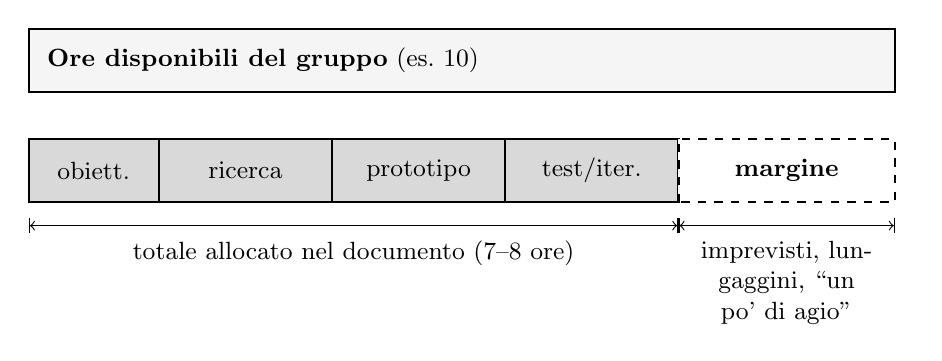
\begin{tikzpicture}[font=\small, x=1.1cm, y=1cm]
  % ore disponibili
  \draw[thick, fill=gray!8] (0,1.4) rectangle (10,2.2);
  \node[anchor=west] at (0.1,1.8) {\textbf{Ore disponibili del gruppo} (es.\ 10)};
  % ore allocate
  \draw[thick, fill=gray!30] (0,0) rectangle (1.5,0.8);
  \node at (0.75,0.4) {obiett.};
  \draw[thick, fill=gray!30] (1.5,0) rectangle (3.5,0.8);
  \node at (2.5,0.4) {ricerca};
  \draw[thick, fill=gray!30] (3.5,0) rectangle (5.5,0.8);
  \node at (4.5,0.4) {prototipo};
  \draw[thick, fill=gray!30] (5.5,0) rectangle (7.5,0.8);
  \node at (6.5,0.4) {test/iter.};
  \draw[thick, dashed, fill=white] (7.5,0) rectangle (10,0.8);
  \node at (8.75,0.4) {\textbf{margine}};
  \draw[|<->|] (0,-0.3) -- (7.5,-0.3)
    node[midway, below=2pt] {totale allocato nel documento (7--8 ore)};
  \draw[|<->|] (7.5,-0.3) -- (10,-0.3)
    node[midway, below=2pt, text width=3cm, align=center] {imprevisti, lungaggini,
    ``un po' di agio''};
\end{tikzpicture}
\caption{La ``enorme regola'' del documento: la somma delle ore allocate alle fasi
deve restare sotto le ore disponibili. Le fasi e le proporzioni sono solo
illustrative.}
\label{a9:fig:margine}
\end{figure}

\paragraph{Approfondimento: il margine e il ``buffer''.} Il consiglio di Beatrice ha
un equivalente preciso nella gestione dei progetti: il \emph{buffer}, una riserva di
tempo non assegnata a nessuna attività, che assorbe gli scarti senza far saltare la
scadenza. Nei metodi agili lo stesso principio si traduce nel non riempire mai lo
\emph{sprint} al 100\% della capacità del team. Schell, in \emph{The Art of Game
Design}, osserva che i progetti di giochi sono particolarmente esposti agli
sforamenti, perché il lavoro di design è iterativo per natura e non si sa in anticipo
quanti cicli di test serviranno: proprio per questo il margine non è un lusso, ma la
condizione per poter iterare.

% ---------------------------------------------------------------------
\section{Emozioni, meccaniche e flusso: esplicitare}
\label{a9:sec:esplicitare}

Le voci successive del documento sono cose che la classe ``sa già tantissimo'': uno
spazio per ricordarsi di \textbf{esplicitarle}.

\paragraph{Le emozioni (punto 4).} Il percorso sull'\emph{emotional design} è già
stato fatto. Il punto 4 serve solo a ricordare di scrivere quale emozione si è
scelta, perché può succedere che durante il brainstorming ci si concentri molto
sull'obiettivo (``magari decidete di fare un'escape room per divulgare i funghi e un
viaggio nel bosco, come avevamo deciso nella lezione precedente''), si sia ``molto
presi dal tema'' e ci si dimentichi di dare spazio alla parte emotiva. ``Non è una
cosa in più, è proprio solo per dare lo spazio''.

\paragraph{Le meccaniche e il flusso (punto 5).} Lo stesso vale per le meccaniche: si
è già visto che serviranno meccaniche che portano a fare delle cose, e un
\textbf{flusso di gioco} (``lo trovate anche a conclusione del documento sul design
sprint''). Esplicitarle non vuol dire ``sono queste, le manteniamo così per sempre'':
vuol dire ricordarsi di metterle nero su bianco, perché ``magari le abbiamo molto
chiare, ma non le abbiamo esplicitate'', e averle scritte serve al gruppo e ai
designer ``per poter vedere cosa sta succedendo''. Lo stesso vale per il
\textbf{flusso del giocatore} e per le \textbf{dinamiche} che nascono dalle
meccaniche. Nel documento (``in piccolino piccolino, che non so neanche se si
legge'') c'è una divisione in colonne: la \textbf{meccanica}, \textbf{che cosa fa il
giocatore} in quella meccanica e \textbf{che cosa voglio che provi}.

% ---------------------------------------------------------------------
\section{Il percorso dell'utente}
\label{a9:sec:percorso}

\slidefig{img/AGD/agd9-percorso}{Il percorso dell'utente e il primo prototipo nel documento di project management.}{slide \emph{Esperienze ludiche 1}}{fig:agd9-percorso}


Il \textbf{percorso dell'utente} era rimasto in sospeso la volta precedente (``non
abbiamo avuto il tempo di affrontarlo con calma''), e ora Beatrice gli dedica ``un
attimino''. È un termine che viene ``nuovamente'' dal \textbf{marketing}: è ciò che
fa l'utente per arrivare a un obiettivo desiderato. Nei giochi è molto più difficile
da fare che nel marketing, ``ma vi invito a farlo'': soprattutto alle prime armi, ma
anche dopo, perché ``spesso non c'è il tempo di esplicitarlo, ma bisognerebbe''.

\paragraph{Banalmente, dall'inizio.} Si tratta di rendere esplicito che cosa fa la
persona giocante dall'inizio alla fine, ``ma banalmente, davvero''.
\begin{itemize}
  \item In un gioco da tavolo, la prima cosa che farà è \textbf{sedersi al tavolo}.
        ``È così?''. O il gioco è uno di quelli in cui si sta \textbf{in piedi} di
        fianco al tavolo\footnote{La trascrizione dice ``come soccuadro'', un titolo
        che non è possibile ricostruire con certezza; il senso è un gioco da tavolo
        che si gioca in piedi.}.
  \item Oppure la prima cosa è \textbf{aprire un regolamento cartaceo} e sfogliarne le
        parti; la seconda è \textbf{guardare i componenti}, e probabilmente
        stenderli sul tavolo per vederli tutti.
  \item In un \textbf{gioco pervasivo} in città, la prima cosa sarà uscire di casa e
        aprire il link ricevuto, oppure uscire con ``la scatoletta di gioco'' e
        trovare un posto dove appoggiarsi.
\end{itemize}
Questo è l'inizio. Poi c'è il \textbf{percorso del gioco}: la prima cosa è mettere la
pedina sul punto 1 del tabellone, la seconda è pescare una carta, e così per cinque
turni in cui succedono $N$ cose; poi la \textbf{conclusione}: il giocatore ha fatto
una serie di passaggi e il gioco finisce.

\paragraph{A che cosa serve: il passaggio mancante.} Il percorso dell'utente serve a
verificare che ci sia una \textbf{linearità}, e va fatto \textbf{prima} di arrivare
alla conclusione della progettazione, ``perché ci serve a capire cosa succede davvero
alla persona giocante''. È qualcosa che si spera venga ``per forza di cose''
progettando, ma esplicitarlo aiuta a ragionare: ``spesso ci immaginiamo che succedano
delle cose, e poi manca un passaggio per farle succedere''. Banalmente: un'istruzione
in più, una pedina in più, \textbf{la penna}. ``Gli diciamo: scrivi, prendi appunti.
Ma non ha la penna, e ormai è in strada a giocare, e nessuno gli ha detto di prendere
la penna''.

\paragraph{Prima del test.} Quasi sicuramente il percorso andrà rivisto dopo il test.
Ma prima di arrivarci, ``alleniamoci a vedere tutti i passaggini che la persona mette
in fila per arrivare a iniziare e finire il nostro gioco''.

\paragraph{Approfondimento: la \emph{customer journey} e la lente del giocatore.}
Il ``percorso dell'utente'' è la \emph{user journey} (o \emph{customer journey})
della progettazione di servizi e del marketing: la sequenza dei punti di contatto tra
una persona e un prodotto, dall'avvicinamento all'uscita. Applicato a un gioco
analogico, include ciò che i designer tendono a dimenticare perché lo danno per
scontato: aprire la scatola, leggere il regolamento, preparare il tavolo, riporre i
componenti. Schell suggerisce di guardare il gioco con gli occhi di chi lo incontra
per la prima volta (la sua ``lente del giocatore''), e osserva che molti problemi di un
gioco non stanno nelle regole ma nei momenti che le precedono e le seguono.
L'esempio della penna di Beatrice è esattamente uno di questi.

% ---------------------------------------------------------------------
\section{Il primo prototipo: fisso, provvisorio, non ancora}
\label{a9:sec:prototipo}

Poi si arriva alla \textbf{costruzione del primo prototipo}. Anche questo, immagina
Beatrice, verrà ``in modo abbastanza automatico'': fare l'elenco di che cosa si vuole
e che forma deve avere. I componenti e le meccaniche sono già stati decisi nel design
sprint e nella prima parte del documento; qui si \textbf{esplicitano}. Se il
componente sono delle carte, quante carte e come. Se è un \textbf{quadernino}, bisogna
capire ``di quante pagine'', dove mettere le grafiche, che cosa deve contenere.

\paragraph{Le tre domande.} Ma la parte importante (``e questo è importantissimo'')
è decidere, per ogni elemento, in quale di tre categorie sta (Beatrice legge le tre
domande della slide una dopo l'altra, e se ne scusa):
\begin{enumerate}
  \item che cosa \textbf{deve essere contenuto necessariamente} nel prototipo, e
        fissato;
  \item che cosa si può \textbf{lasciare provvisorio};
  \item che cosa \textbf{non si deve ancora realizzare}.
\end{enumerate}

\paragraph{Necessario.} In un gioco in forma di libretto, o in un'escape room in
libretto, le istruzioni di gioco e gli enigmi, con il loro funzionamento, vanno
avuti già nella fase prototipale: ``sono una cosa necessaria da avere''. Le
illustrazioni di contorno, o i \emph{copy} specifici delle pagine, si possono
sistemare in un secondo momento.

\paragraph{Non tutto testato, ma l'indispensabile sì.} ``Io credo ve l'abbiano già
detto'', e Beatrice lo risottolinea: lo scopo non è avere subito uno strumento
playtestato e funzionante su tutto, su cui si è ragionato ``in modo cristallino''. È
anzi capire quali cose \textbf{diventano indispensabili}, quelle che, una volta
decise, se cambiano ``vi cambia tutto il gioco''. L'esempio: un'escape room con
\textbf{tre enigmi principali}. Si testano prima quelli, poi si prosegue nella
costruzione. Se invece si prepara tutto il resto (la storia che racconta gli enigmi,
le grafiche ``fatte a modino'') e poi uno dei tre enigmi non funziona al test, bisogna
rifare un lavoro importante.

\paragraph{Il criterio del provvisorio.} La scelta si fa con una domanda: \emph{se
questa cosa cambia, dovrò cambiare tutte le cose che le stanno attorno?} Se la
risposta è sì, le cose attorno vanno tenute \textbf{provvisorie} ``per un attimo''.
È un lavoro che verrà più facile con l'esperienza, ma intanto conviene spendere un
po' di tempo a valutare che cosa va fatto e testato subito e che cosa si può
sistemare dopo.

\paragraph{Che cosa non realizzare ancora.} Che cosa non serve per playtestare e
raccogliere dati? Magari \textbf{la copertina}; ``o magari sì, perché uno degli enigmi
è nascosto nella copertina''. Oppure un gioco di carte molto ricco di meccaniche, con
una narrazione che è più un \emph{setting} che un'esplorazione narrativa: forse
\textbf{le illustrazioni} non servono ora, ``posso farlo proprio senza
illustrazioni''. Di ciò che è necessario, poi, si distingue di nuovo che cosa deve
essere già fisso da testare e che cosa può restare provvisorio, ``perché se cambia
qualcosa non dobbiamo rifare tutto il lavoro da capo'' (figura~\ref{a9:fig:prototipo}).

\begin{figure}[htbp]
\centering
\begin{tikzpicture}[
    font=\small,
    q/.style={draw, thick, rounded corners, fill=gray!10, text width=4.4cm,
      align=center, inner sep=5pt},
    r/.style={draw, rounded corners, text width=3.4cm, align=left, inner sep=5pt},
    >=Latex
  ]
  \node[q] (q1) at (0,0) {Serve per playtestare e raccogliere dati?};
  \node[r, dashed] (no) at (5.2,0) {\textbf{Non ancora}\\ es.\ copertina,
    illustrazioni di un gioco di meccaniche};
  \node[q] (q2) at (0,-2.2) {Se cambia, devo cambiare tutto ciò che le sta
    attorno?};
  \node[r, fill=gray!25] (fix) at (-4.4,-4.4) {\textbf{Necessario e fisso}\\ es.\
    i tre enigmi principali, le istruzioni del libretto: si testano subito};
  \node[r] (prov) at (4.4,-4.4) {\textbf{Provvisorio}\\ es.\ storia attorno agli
    enigmi, grafiche ``a modino'', \emph{copy} delle pagine};
  \draw[->] (q1) -- node[above]{no} (no);
  \draw[->] (q1) -- node[right]{sì} (q2);
  \draw[->] (q2.south west) -- node[above left]{sì: è il nucleo} (fix);
  \draw[->] (q2.south east) -- node[above right]{dipende dal nucleo} (prov);
\end{tikzpicture}
\caption{Le tre domande sul primo prototipo, come le pone Beatrice: che cosa non
realizzare ancora, che cosa fissare e testare subito, che cosa tenere provvisorio.
Ricostruzione schematica.}
\label{a9:fig:prototipo}
\end{figure}

\paragraph{Approfondimento: il prototipo che risponde a una domanda.} La regola di
Beatrice è la stessa che Schell formula nel capitolo sui prototipi di \emph{The Art
of Game Design}: ogni prototipo deve rispondere a una domanda, e non deve contenere
niente che non serva a rispondervi. Nel lessico dello sviluppo software, il nucleo
da fissare per primo è ciò da cui ``dipendono'' le altre parti: costruire prima le
dipendenze e poi ciò che dipende da loro evita di rifare il lavoro a cascata. Gli
enigmi di un'escape room sono l'esempio perfetto, perché storia e grafica vengono
scritte \emph{attorno} a loro.

% ---------------------------------------------------------------------
\section{Playtest e iterazione}
\label{a9:sec:iterare}

Sul \textbf{playtest} Beatrice chiede se la classe abbia già fatto la lezione di
Ruggero sull'argomento. No. Allora, ``per tempo'', salta completamente quelle slide:
la lezione di Ruggero farà ``un bellissimo approfondimento'' e renderà
``cristallina'' anche la slide appena raccontata. Dice solo che quella slide
corrisponde a una parte del documento in cui mettere le cose principali da tenere a
mente quando si playtesta: ``di nuovo, uno spazio per ricordarci di tenerle a mente''.
Come tutto il documento, non è obbligatorio compilarlo.

\paragraph{Il ciclo.} Lo stesso vale per l'\textbf{iterazione}, che Ruggero
spiegherà nella lezione sul playtest e che la classe ha ``già un po' intuito'' da
tutti i discorsi fatti. Di base, il percorso di creazione di un gioco è
\textbf{creare} (inventare, progettare), \textbf{playtestare}, \textbf{raccogliere
dati} e poi \textbf{iterare} sui dati raccolti (figura~\ref{a9:fig:ciclo}).

\paragraph{L'esempio della scritta gigante.} Si è scritto ``in caratteri cubitali''
che il gioco si gioca \textbf{al buio}, e nessuna delle persone che lo testano legge
quella frase: lo giocano tutti alla luce. ``C'è qualcosa di enorme che non va''. Si
deve iterare su quella voce: fare domande (``perché non hai letto questa scritta
gigante? Cosa è successo?'') e soprattutto \textbf{osservare} mentre le persone
giocano. Magari la scritta è in un angolo dove l'occhio non cade, ``e quindi lo
vediamo non tanto parlando con la persona, ma osservando mentre legge i nostri
materiali di gioco''. Raccolto il dato, si modifica il gioco in base al dato: ``e
questa modifica è iterare''.

\paragraph{Infinite volte.} ``Questo ciclo si fa infinite volte'', tutte le volte che
si può finché c'è tempo per testare: ``questa è proprio una cosa cristallina che
dovete portarvi a casa''.

\begin{figure}[htbp]
\centering
\begin{tikzpicture}[
    font=\small,
    st/.style={draw, thick, rounded corners, fill=gray!10, minimum width=3cm,
      minimum height=0.9cm, align=center},
    >=Latex
  ]
  \node[st] (c) at (90:2.2) {Creare\\ \footnotesize inventare, progettare};
  \node[st] (p) at (0:3.3) {Playtestare};
  \node[st] (d) at (-90:2.2) {Raccogliere dati\\ \footnotesize domande e
    osservazione};
  \node[st] (i) at (180:3.3) {Iterare\\ \footnotesize modificare il gioco};
  \draw[->, thick] (c) to[bend left=20] (p);
  \draw[->, thick] (p) to[bend left=20] (d);
  \draw[->, thick] (d) to[bend left=20] (i);
  \draw[->, thick] (i) to[bend left=20] (c);
  \node[align=center, text width=3.6cm] at (0,0) {\footnotesize ``infinite volte'',
    finché c'è tempo per testare; a volte cambia anche l'obiettivo};
\end{tikzpicture}
\caption{Il ciclo di progettazione come lo riassume Beatrice, in attesa della lezione
di Ruggero sul playtest.}
\label{a9:fig:ciclo}
\end{figure}

\paragraph{Quando cambia tutto.} Nell'iterazione capiterà anche di accorgersi che c'è
qualcosa ``di molto grosso'' che non va. Si è deciso di fare un'escape room per
divulgare ``tutta la scienza dei funghi'' (``io dei funghi non so nulla, spero di non
stare usando terminologie incorrette''), e dopo il quarto test ci si rende conto che
non funziona come escape room: le persone, mentre giocano, ``stanno ruolando quasi'',
ragionano e vivono molto di più la parte narrativa. Se così fosse, ``non abbiamo
paura di cambiare anche l'obiettivo del gioco, anche la forma del gioco'', sempre in
linea con i vincoli. Se il committente ha chiesto un'escape room sui funghi, si dovrà
cambiare altro; e se non c'è il tempo di modificare, ci si tiene quel gioco ``per
ora''.

\paragraph{Niente è buttato.} Ma la \emph{forma mentis} è: ``non abbiamo paura di
perdere del lavoro mentre progettiamo''. Se in iterazione funziona meglio qualcosa
che non si era valutato, lo si segue, perché ``quello che scartate in un gioco vi
servirà quasi sicuramente in un altro gioco che progetterete più avanti''. Non nella
stessa forma, ma ci si sarà già allenati a un tipo di pensiero, di meccanica, di
dinamica, e lo si sarà perfino già testato: è già nel proprio ``bagaglio formativo e
professionale''. ``Quindi non abbiate paura di seguire il cambiamento che
l'iterazione vi invita a fare, che i vostri playtester, che le vostre persone vi
invitano a fare''.

% ---------------------------------------------------------------------
\section{Documentare sempre}
\label{a9:sec:documentare}

``E dovremmo essere verso la fine, così sto nei tempi''. La voce successiva è
\textbf{documentare sempre}. Durante il corso non ci sarà molto tempo per farlo,
anche se sarà necessario per il playtest. Ma fuori dal corso Beatrice invita a
documentare tutto:
\begin{itemize}
  \item fare \textbf{foto} ai giocatori;
  \item chiedere \textbf{feedback scritti} ``che siano quasi delle recensioni'';
  \item tenere dei propri \textbf{giornali di game design};
  \item registrare \textbf{audio} in cui appuntarsi il proprio processo creativo.
\end{itemize}

\paragraph{A che cosa serve.} A due cose. A \textbf{vedere come si lavora},
acquisendo più esperienza su di sé; e a \textbf{poterlo raccontare fuori}. E
raccontare come si lavora, anche senza autopubblicarsi, ``è qualcosa che vi apre più
porte, spesso e volentieri'', più di tanti titoli sul curriculum o sul portfolio, più
dei ``contatti giusti'': ``può essere qualcosa che davvero è molto, molto potente''.
Quindi: raccogliere i dati e raccontarli fuori quando si può.

\paragraph{Il rimando al GDPR.} Quel ``quando potete'' ha un limite normativo, e
Beatrice lo anticipa: c'è ``una grossa parte normativa'', il \textbf{GDPR}, che si
vedrà più avanti nelle slide di oggi, con ``un piccolo strumento'' per poter
ripubblicare i dati che coinvolgono altre persone, cioè le proprie persone giocanti
(sezione~\ref{a9:sec:burocrazia}).

% ---------------------------------------------------------------------
\section{Monitorare: che tipo di stimatori siamo}
\label{a9:sec:monitoraggio}

``Documentare sempre lo abbiamo detto; poi monitoriamo''. Si prende la lista di tutte
le voci a cui si erano attribuite delle ore e si guarda se davvero ci si sono messe
quelle ore. ``Questa cosa sul subito non serve praticamente a niente'': ci si ferma e
si osserva che cosa è successo. Ma col tempo, raccolti dati su almeno \textbf{due o
tre progetti}, con lo stesso gruppo o come singole persone, si potranno fare stime più
realistiche.

\paragraph{Chi stima largo, chi stima stretto.} Se su tre progetti si è sempre
stimato più tempo del necessario, si sa di essere persone che \textbf{stimano alla
larga}. Se invece, ``come succede sempre a me'', si stima \textbf{più stretto} (``dite
ci metto tre ore e poi ce ne metto cinque''), si sa che in futuro conviene correggere:
``a me verrebbe da mettere tre ore su questa voce, ma non gliene metto tre, perché so
già da dati pregressi che mi conviene mettergliene cinque, sei, un po' di più''.

\paragraph{Le domande del monitoraggio.} Il documento dà ``lo spazio fisico'' per
rispondere ad alcune domande, ``non sono obblighi'' (Beatrice qui accelera, ``ora
vado un po' più veloce''): che cosa ha funzionato; che cosa ha fatto \textbf{perdere
tempo}; che cosa è stato \textbf{sottostimato}.

% ---------------------------------------------------------------------
\section{La stima: il 20\% in più e la stima di pancia}
\label{a9:sec:stima}

\slidefig{img/AGD/agd9-stima}{La formula per stimare il tempo, e perché non è una verità.}{slide \emph{Esperienze ludiche 1}}{fig:agd9-stima}


La \textbf{formula per stimare il tempo} Beatrice la salta ``a piè pari''. ``In
estrema sintesi'': \textbf{mettete sempre un 20\% in più} di quello che immaginate.
Se il gruppo è \textbf{nuovo} e non ha mai lavorato insieme, ``anche un po' di più del
20\%''. E la formula va comunque verificata facendo diversi progetti: ``non è una
regola statistica, va valutata sulle vostre cose''.

\paragraph{Quante ore mettere se non l'ho mai fatto.} Resta la domanda più concreta:
se non si è mai scritto un regolamento, quante ore mettere nella stima? L'invito è
questo.
\begin{enumerate}
  \item Se si hanno \textbf{dati pregressi}, cercare di ricordarli, anche se non sono
        stati annotati: ``ci avete messo 4 ore a scrivere l'ultima tesina
        dell'università, oppure l'ultima ricerca online, oppure l'ultimo post su
        Instagram''. Si prende il dato \textbf{più simile} all'attività da fare.
  \item Se non c'è nessun dato simile, \textbf{non si lascia a zero}: si fa una
        \textbf{stima di pancia}, ``ma comunque ipotizziamo''.
\end{enumerate}
La stima di pancia serve al ragionamento di prima: capire se si tende a stimare largo
o stretto, come singole persone. ``Tancredi, Beatrice, Tiziana'': ``Tancredi magari
stima in eccesso, Tiziana stima più stretto, Beatrice stima più stretto''. Ma è
importante cominciare a notarlo, ``e non possiamo notarlo se non facciamo una stima
iniziale, quindi di pancia''.

\paragraph{Perché vale la pena.} Tornando a una slide saltata (``questo è importante
in realtà, quindi ve lo dirò''), Beatrice spiega perché sapere quanto ci si mette è un
investimento. Non sembrerà utile subito, perché non incide direttamente sulla
progettazione, soprattutto nei primi progetti; ma col tempo è un'informazione
essenziale:
\begin{itemize}
  \item per \textbf{lavorare con altre persone}: si sa quanto ci si mette e si
        comincia a capire quanto ci mettono gli altri;
  \item per avere una \textbf{stima realistica}: ``so che ci abbiamo messo tanto
        tempo a fare un gioco in questo team di tre persone che non aveva mai
        lavorato insieme''. ``È come chiedere dei preventivi, tutto sommato'': senza
        nemmeno un appiglio numerico non si sa da dove partire;
  \item per \textbf{valutare le proposte}: se si viene invitati a collaborare a un
        gioco e viene chiesto di fare in due mesi un intero gioco di ruolo con
        diversi \emph{branching} narrativi, o un librogame con molte illustrazioni,
        si sa che non è possibile, e si può scegliere consapevolmente se provarci lo
        stesso o dire ``secondo me questi tempi non ci stanno'';
  \item sul lato lavorativo, per capire se le proposte che arrivano sono sensate e,
        ``ancora di più'', \textbf{quanto farsi pagare} da \emph{freelance}, ``un tema
        di cui si parla ancora troppo poco''. Spesso viene proposto un
        \textbf{forfait} ``che non ha né capo né coda'', e invece va valutato sulle
        ore che servono davvero. La stima diventa uno \textbf{strumento di
        contrattazione}: si sa già quante ore servono, e si può dire con certezza se
        una cosa si può fare o no.
\end{itemize}

\paragraph{La regola più importante.} ``L'ho già detto, lo ripeto in modo ancora più
esplicito'': tutto questo è un \textbf{allenamento}. I calcoli non saranno mai
``matematici, precisi al millimetro'': servono ad avere più consapevolezza ``di come
stare in questo mondo e di come funzioniamo''.

\paragraph{L'esercizio per il corso.} L'invito per il project work è stimare tutte le
voci viste, in \textbf{due momenti}: prima ognuno da solo (quanto ci metterò io), poi
il confronto nel gruppo. E poi monitorare entrambi i livelli. ``E ci siamo! Sono
perfettamente nei tempi che pensavo di utilizzare''.

\paragraph{Perché un gioco concluso.} Il documento resta a disposizione di tutti,
da ``sbirciare'' senza alcun obbligo: è un'indicazione per riuscire a \textbf{concludere un
gioco} in questi due mesi, ``perché a noi interessa non un gioco perfetto, ma un gioco
concluso'', che serva per allenarsi su tutto: il project management, ma soprattutto
la progettazione e la creazione. ``E se il gioco non lo finite, il rischio è che
perdete una grossa parte della formazione che può darvi questo corso''. Tenere conto
del tempo e delle risorse è ``un vantaggio vostro''.

\paragraph{Approfondimento: stimare per confronto.} Il metodo di Beatrice (stimare
prima da soli, poi confrontarsi nel gruppo) ricorda le tecniche di stima collettiva
dello sviluppo agile, come il \emph{planning poker}: ognuno stima in segreto, poi le
stime si rivelano insieme, e le differenze più ampie diventano l'occasione per
discutere ciò che uno ha visto e l'altro no. Stimare in privato prima del confronto
evita l'effetto ``àncora'' della prima cifra detta ad alta voce. E il 20\% in più è un
modo semplice di includere il \emph{buffer} di cui si è detto
(sezione~\ref{a9:sec:margine}) nella stima stessa.

% ---------------------------------------------------------------------
\section{Semplice è meglio}
\label{a9:sec:semplice}

\slidefig{img/AGD/agd9-semplice}{Semplice è meglio.}{slide \emph{Esperienze ludiche 1}}{fig:agd9-semplice}


L'ultima slide (``in ambito lavorativo poi lo leggete voi'') contiene una regola che
Beatrice vede spesso ``non abbastanza valutata'': \textbf{semplice è meglio}. Non vuol
dire ``fate giochi al ribasso'': ``seguite i vostri sogni, seguite quello che vi va di
progettare'', soprattutto in contesti senza committente e senza vincoli stringenti. Ma
quando si fa il percorso dell'utente e si testa, la semplicità conviene a due
``realtà'': agli \textbf{utenti}, le persone che giocheranno, e ai \textbf{designer},
``per non complicarvi la vita''.

\paragraph{La domanda da farsi ogni tanto.} Nel pratico, Beatrice l'ha messa ``proprio
come domanda esplicita'':
\begin{quote}
Qual è la versione più semplice dell'idea che ho avuto, che riesce comunque a far
vivere alla persona giocante l'esperienza che io voglio creare?
\end{quote}
È un'indicazione per districarsi dai momenti complicati, quando si perde la rotta; ma
``in linea generale è un'indicazione che diventa proprio un buon principio di
design''.

\paragraph{Approfondimento: la lente dell'eleganza.} Schell dedica a questa idea la
``lente dell'eleganza'': un gioco elegante è quello in cui ogni elemento ha più di
uno scopo e nulla è superfluo, e la domanda da farsi è quali elementi si potrebbero
togliere senza perdere l'esperienza. È la stessa domanda di Beatrice, posta dal
lato opposto: lei chiede qual è la versione più semplice che conserva l'esperienza,
Schell chiede che cosa si può togliere senza perderla.

% ---------------------------------------------------------------------
\section{Il commento della classe}
\label{a9:sec:feedbackpm}

``Ok, abbiamo concluso la lezione della volta scorsa''. Beatrice chiede cinque minuti
di riflessione: com'è andata questa parte, ``che era completamente nuova, e siete le
prime persone a vederla in questa forma''?

\paragraph{Utile o superflua?} Tiziana non ha domande, ``ti dico la verità'', ma
trova molto comodo avere un documento riassuntivo con tutti i passaggi, e apprezza
``tantissimo'' le indicazioni ``da chi ha già fatto'', soprattutto sulla
programmazione dei tempi e sulla documentazione: ``ne farò tesoro''. Beatrice spiega
perché lo chiede: uno dei suoi dubbi, inserendo questa parte, era che fosse
superflua. Al gruppo dell'anno precedente serviva, ``però magari è superflua''. Vuole
sapere se è qualcosa a cui si sarebbe arrivati da soli o se ``vale un'oretta di questo
corso''. Un altro studente è d'accordo con Tiziana: sarà utile, anche se deve ancora
guardarsi il documento con calma per capire come applicarlo.

\paragraph{Il questionario di fine corso.} Beatrice ricorda (e scopre che non era
stato detto) che a fine corso ci sarà un \textbf{questionario}, uno spazio in cui
raccontare che cosa ha funzionato e che cosa no, che cosa è piaciuto e che cosa no.
Invita a parlarne anche per questa parte nuova: ora la si è vista ``a volo
d'aquila'', ma si vedrà se servirà in fase di progettazione.

\paragraph{Un taglio sul lavoro.} Aggiunge un'altra cosa su cui chiede un parere: nelle
sue lezioni ha accentuato, più dei colleghi forse, ``la parte un po' più sul lavoro'',
cioè il ragionare già in ottica di lavorare nel settore. ``Anche qui vi invito a dirmi
a voce se qualcosa non vi torna, che effetto vi fa''. E la parte successiva va proprio
in quella direzione.

% ---------------------------------------------------------------------
\section{Esperienze ludiche 2: due strumenti invece di una carrellata}
\label{a9:sec:esperienze2}

Beatrice cambia presentazione: ``Esperienze ludiche 2'', ``un po' una miscellanea di
varie cose''. E promette di tenere i tempi, ``visto che vi ho fatto tutta questa cosa
sui tempi, provo a fare la brava''.

\paragraph{Perché non una carrellata.} Voleva raccontare un po' di strumenti usati nel
settore, ma si è accorta che rischiava di diventare ``una carrellata di strumenti di
diverso tipo'', senza l'indicazione per andarli a vedere nel dettaglio. Era successo lo
stesso con il design sprint: la lezione stava nascendo come un'altra carrellata, e ha
preferito far \textbf{esperire} uno strumento solo, ``ma con ordine'', così che chi si
trova bene possa riusarlo; per chi non si trova, ci sono le dispense con altre
modalità di brainstorming e altri strumenti. Qui fa lo stesso ragionamento: invece di
una carrellata, ``un volo veloce su due strumenti'', di cui uno è ``sempre nominato
nei manuali'': il Game Design Document.

% ---------------------------------------------------------------------
\section{Il Game Design Document}
\label{a9:sec:gdd}

Beatrice chiede una \emph{reaction} a chi non ha mai sentito il termine \textbf{Game
Design Document} (uno studente non ha capito la domanda: ``forse parlo troppo in
fretta''). Alcune manine si alzano, ``sono manine di reaction, non sono domande''; e
``c'è un po' di persone che l'hanno sentito molto bene''.

\paragraph{Che cos'è.} Di base, ``lo dice un po' il titolo'', è un documento che
\textbf{racconta più o meno tutto il gioco}. Prende forme molto diverse ed è usato
soprattutto nell'\textbf{industria videoludica}. ``Immaginate una sorta di Bibbia del
gioco'': di qualunque gioco (``ti racconta sempre che esista, di Cluedo, un game design
document'') racconta, in fase di progettazione, gli obiettivi, come funziona, le varie
fasi, perché sono state fatte certe scelte, la parte di \emph{art} e tutto il resto.
``Una grande Bibbia che, se tu leggi dall'inizio alla fine, hai una chiara visione del
gioco''.

\paragraph{Che cosa succede davvero nell'analogico.} È un documento progettuale che,
``nello stato attuale dell'industria analogica'', non si usa quasi mai: la maggior
parte delle volte \textbf{si lavora direttamente sul regolamento}. Uno studente chiede
se si parla dell'industria analogica italiana, ``perché immagino che all'estero
funzioni diversamente''. Beatrice precisa: dice quello che sa ``per certo''
sull'industria italiana, in cui è uno strumento ``che non viene utilizzato granché''.

\paragraph{Perché saperlo comunque.} Ci tiene a parlarne perché viene raccontato come
strumento necessario nei \emph{game studies}, ``cioè in tutta la parte accademica,
tutta la parte di manuali su game design'': va saputo che esiste. E nel mondo dei
\textbf{bandi}\footnote{La trascrizione dice ``nel mondo della bandistica''; dal
contesto si tratta dei bandi di finanziamento.} si usa ancora, ``proprio per
raccontare il progetto''. Non ha un'unica forma: racconta tutto il gioco, o la parte
che serve raccontare ``in base a chi vi sta chiedendo questo documento''.

\paragraph{Il desiderato e la realtà.} Nel mondo ideale il GDD sarebbe anche un
documento di lavoro \textbf{mutevole}, che chiunque può leggere e usare per lavorare
sul gioco: il punto di riferimento per tutti i professionisti che collaborano allo
stesso titolo. ``Nel mondo pratico non funziona così'', e si ragiona ancora molto ``di
riunioni, di documenti un po' sparpagliati''. A Beatrice interessa dire ``quello che
viene raccontato, quello che è il desiderato e quella che è la realtà'', e che si
ricordi la terminologia. ``Fine''.

\paragraph{Che cosa chiede il corso.} Per il corso, ricorda che cosa è stato fatto
l'anno prima (``poi mi correggeranno in caso i colleghi''): non viene chiesto un
documento di lavoro, ``è proprio il gioco''. Non c'è nessuna indicazione su come
lavorare o su che cosa produrre per mettersi d'accordo: il design sprint e il
documento sui tempi danno già una direzione, che può diventare ``una lavagna Miro, un
documento condiviso su Drive, una cartella condivisa con vari documenti''. ``Vi lascio
piena interpretazione di come volete collaborare''.

\paragraph{Approfondimento: il GDD nei manuali.} Il Game Design Document è centrale
nella manualistica sul videogioco, dove nasce come contratto tra i reparti di uno
studio. Lo stesso Schell, però, mette in guardia dal documento-monolite: nel
capitolo sulla documentazione osserva che non esiste un formato unico, che i documenti
servono soprattutto come \emph{memoria} e come \emph{comunicazione}, e che un
documento che nessuno legge e nessuno aggiorna non svolge nessuna delle due funzioni.
È la distanza tra ``desiderato'' e ``realtà'' di cui parla Beatrice. Molti studi,
anche nel digitale, sono passati a documenti più brevi e vivi (\emph{one-page
design}, \emph{wiki} interne).

% ---------------------------------------------------------------------
\section{L'Experience Canvas}
\label{a9:sec:canvas}

\slidefig{img/AGD/agd9-canvas}{L'Experience Canvas.}{slide \emph{Esperienze ludiche 2}}{fig:agd9-canvas}


Il secondo strumento è per quando ``il gruppo non sa bene che direzione prendere'',
se si perde la direzione comune. Beatrice lascerà nella cartella condivisa, tra gli
allegati, un esempio: l'\textbf{Experience Canvas}, che deriva dai \textbf{Business
Model Canvas}, ``strumenti per mettere ordine a progetti complessi''. L'ha ricreato
apposta come posto dove riassumere \textbf{tutte le decisioni} che si prendono.

\paragraph{Come si usa.} Secondo lei il documento sui tempi basta già per ``fare un
recapone'' di ciò che succede nel gioco. Ma se serve più visualità, o un altro modo di
lavorare, l'Experience Canvas è ``un documento anche molto impostato'' e ``molto, molto
comodo''. Ha già dei piccoli esempi di compilazione, e una versione completamente
vuota da riempire. È un documento di \textbf{Canva} (``quindi non il Canvas, ma
proprio Canva, il software che abbiamo usato la volta scorsa''), da copiare nel
proprio account e riempire in condivisione con il gruppo. ``È un documento operativo,
nulla di più, non è un obbligo utilizzarlo. Se vi è utile usatelo, se non vi è utile,
via nel sole''.

\paragraph{Approfondimento: dal Business Model Canvas ai canvas di design.} Il
\emph{Business Model Canvas} di Alexander Osterwalder riassume un modello di business
in nove riquadri su un unico foglio (clienti, proposta di valore, canali, risorse,
costi\ldots), e ha ispirato molti ``canvas'' derivati, anche per il game design: il
pregio comune è costringere a una risposta breve per ogni voce e a vedere tutte le
voci insieme, così che le incoerenze saltino all'occhio. Il contenuto preciso
dell'Experience Canvas di Beatrice non è descritto a lezione.

% ---------------------------------------------------------------------
\section{Le tre grandi domande}
\label{a9:sec:tredomande}

E se non si usa nessuno di questi strumenti (``non il design sprint, non il documento
sui tempi e non questo''), un'indicazione per arrivare a concludere il gioco è
rispondere alle \textbf{tre grandi domande}:
\begin{enumerate}
  \item \textbf{chi gioca?}
  \item \textbf{che cosa gioca}, cioè che forma ha il gioco e che obiettivo ha?
  \item \textbf{come è fatto il gioco?}
\end{enumerate}
``A queste tre cose dovete rispondere. Non sapete rispondere? Non avete concluso il
gioco''. Può sembrare ``una cosa scontata, una stupidata'', ma se ci si perde per
strada sono queste le domande a cui tornare: ``non abbiamo risposto a una di queste
domande? C'è un problema. Quindi dobbiamo tornarci su''. Qualunque documento o
strumento si usi, anche gli appunti su un quadernino, ``a queste tre cose bisogna dare
risposta. Fine di questa parte''.

\begin{figure}[htbp]
\centering
\begin{tikzpicture}[
    font=\small,
    d/.style={draw, thick, circle, minimum size=2.6cm, align=center, fill=gray!10,
      text width=2.2cm},
  ]
  \node[d] (a) at (0,0) {\textbf{Chi gioca?}\\ \footnotesize target, contesto};
  \node[d] (b) at (3.4,0) {\textbf{Che cosa gioca?}\\ \footnotesize forma e
    obiettivo};
  \node[d] (c) at (6.8,0) {\textbf{Come è fatto?}\\ \footnotesize componenti,
    regole, flusso};
  \node[below=0.4cm of b, text width=9cm, align=center] {\footnotesize Se manca una
    risposta, il gioco non è concluso: ``c'è un problema, dobbiamo tornarci su''.};
\end{tikzpicture}
\caption{Le tre grandi domande di Beatrice, valide qualunque strumento usi il
gruppo.}
\label{a9:fig:tredomande}
\end{figure}

% ---------------------------------------------------------------------
\section{Giochi formativi: gamification e game based learning}
\label{a9:sec:formativi}

``Andiamo finalmente ai \textbf{giochi formativi}''. Si parte da due termini:
\textbf{gamification}, che ``ha preso molto piede negli ultimi anni'', e \textbf{game
based learning}. Beatrice chiede chi non li abbia mai sentiti: nessuno alza la mano
per la gamification; per il game based learning, sì, Gianmarco\footnote{La
trascrizione dice prima ``Marco'', poi si corregge in ``Gianmarco''.}.

\paragraph{Un termine improprio.} Beatrice avverte che userà ``giochi formativi'' in
modo un po' improprio, ``perché la vera verità è che non abbiamo neanche ben chiaro,
nel mondo dei Game Studies, come definire un gioco formativo''. È un gioco che cambia
il comportamento? Un gioco che dà informazioni nuove? Che cosa significa nel pratico?
Non entra in tutta questa parte, ``perché diventa una lezione troppo corposa'' (se
interessa, chiede di dirlo nei \emph{feedback}). Le interessa invece dare almeno le
due definizioni, che servono ``sia a livello pratico che, di nuovo, professionale''.

\subsection{La gamification}
\label{a9:sec:gamification}

La \textbf{gamification} è una \textbf{disciplina di progettazione}, ``un'attività
vera e propria'', che usa gli \textbf{elementi} dei giochi all'interno di contesti
che \textbf{non sono giochi}. La parola da tenere a mente è \emph{elementi} (``ve
l'ho messa in grassetto''): livelli, punti, missioni, classifiche, ricompense, ``una
sfilza di cosine''.

\paragraph{Duolingo.} L'esempio più classico è \textbf{Duolingo}, l'app per imparare le
lingue, che usa tantissimo i punti, i livelli e l'interazione con il ``piccolo
gufino'', il personaggio dell'app.

\paragraph{L'esempio della stellina.} Per rendere la cosa tangibile, Beatrice prende
uno ``scopo formativo, passatemi il termine'': \textbf{insegnare i segnali stradali} a
chi sta imparando a guidare. L'attività gamificata è: \emph{ti do una stellina per ogni
segnale stradale che memorizzi, e a 10 stelline sali di livello, oppure raggiungi un
premio}. Questo tocca la \textbf{motivazione estrinseca}.

\subsection{Motivazione intrinseca ed estrinseca}
\label{a9:sec:motivazione}

Beatrice non sa se Ruggero ne abbia già parlato o ne parlerà, e riassume ``tantissimo''
(``è un po' spiegata molto male, ma giusto per capirci'').
\begin{description}
  \item[Motivazione intrinseca.] È interna alla persona. Se sei appassionata di musica
        classica e ti propongo un'attività sulla musica classica, che ci siano un
        gioco, dei \emph{badge}, delle stelline o no, sarai motivata a stare in
        quell'attività, ``perché vado a toccare una tua motivazione intrinseca
        personale''.
  \item[Motivazione estrinseca.] Se invece la musica classica non ti interessa, posso
        metterti livelli, stelline, un premio, \emph{feedback} immediati su che cosa
        funziona e che cosa no del comportamento che stai attuando. Provo a stimolare
        una motivazione \emph{al di fuori di te}: legata ai ``contratti sociali'' in
        cui sei inserito, alle dinamiche di gruppo, alla voglia di scoprire che cosa
        succede nel livello successivo o qual è il premio segreto. E questa
        motivazione ``ti porterà a esplorare un po' la musica classica''.
\end{description}
La gamification punta molto sulla motivazione estrinseca: crea strutture basate su
elementi di gioco ``che ti portano a compiere determinate cose''. Di qui l'esempio
della stellina per ogni segnale memorizzato.

\subsection{Il game based learning}
\label{a9:sec:gbl}

Nel \textbf{game based learning} la parola chiave è \textbf{esperienza}, ``fatta e
finita''. Non sono elementi di gioco sovrapposti a un ambiente che non è di gioco: è
un'esperienza completa, che o crea un'esperienza a sé o, se si sovrappone a un
ambiente non di gioco, ``si intreccia proprio a questo ambiente''.

\paragraph{L'esempio della macchinina.} Stesso obiettivo formativo, i segnali
stradali. L'esperienza completa è: \emph{ti do una piccola macchinina su un tappetone
con un percorso disegnato, e devi compiere il percorso più lungo del tabellone
rispettando tutti i segnali stradali che vedi; a ogni segnale corretto ricevi una
stellina, e la prima persona che arriva a 10 stelline vince un premio}. Ha elementi di
gamification, ``ma una costruzione dell'esperienza''. È un esempio ``molto banale'',
che forse non funzionerebbe nemmeno davvero per formare; serve a far capire la
differenza tra \emph{elementi di gioco piazzati da qualche parte che non è gioco} e
\emph{un'esperienza costruita dall'inizio alla fine} (tabella~\ref{a9:tab:gamification}).

\paragraph{Perché la differenza conta.} Le due modalità ``si possono intrecciare tra
di loro'', ma conoscerne la differenza aiuta a capire quando si sta riuscendo a
raggiungere la \textbf{motivazione intrinseca}, ``che è rarissimo e
difficilissimo'', e quando si lavora sulla motivazione estrinseca, ``punto''.

\begin{table}[htbp]
\centering
\small
\begin{tabular}{@{}p{3cm}p{5.1cm}p{5.1cm}@{}}
\toprule
 & \textbf{Gamification} & \textbf{Game based learning} \\
\midrule
Parola chiave & \textbf{Elementi} di gioco & \textbf{Esperienza} fatta e finita \\
Che cosa fa & Sovrappone punti, livelli, missioni, classifiche, ricompense a un
  contesto che non è un gioco & Costruisce un gioco completo, o lo intreccia al
  contesto \\
Motivazione & Soprattutto estrinseca & Può arrivare all'intrinseca (``rarissimo e
  difficilissimo'') \\
Esempio sui segnali stradali & Una stellina per ogni segnale memorizzato; a 10
  stelline sali di livello o vinci un premio & Una macchinina su un tappetone: il
  percorso più lungo rispettando i segnali, una stellina per segnale, vince chi
  arriva a 10 \\
Esempio reale & Duolingo & (nessuno citato a lezione) \\
\bottomrule
\end{tabular}
\caption{Gamification e game based learning secondo la lezione: due modalità che si
possono intrecciare, ma che conviene distinguere.}
\label{a9:tab:gamification}
\end{table}

% ---------------------------------------------------------------------
\section{La volontarietà: quando un gioco formativo non è un gioco}
\label{a9:sec:volontarieta}

In ambito formativo la distinzione è ``importantissima'' per un motivo che, secondo
Beatrice, il mondo della formazione ludica e interattiva dimentica spesso: le persone
vengono invitate a formarsi con il gioco \textbf{in contesti in cui non stanno
scegliendo appieno di giocare}. Usare un gioco per insegnare a programmare a scuola, e
sceglierlo a casa propria comprandolo su Steam perché si ha voglia di provare
quell'esperienza, ``sono due attività completamente diverse''. Spesso, quando si invita
qualcuno a formarsi con un gioco formativo, ``non sta davvero giocando''.

\paragraph{Da Huizinga in poi.} È da qui che nascono le riflessioni sulle due
discipline: si cerca di usare modalità tipiche del gioco in contesti in cui non c'è
\textbf{volontarietà}, mentre ``ci viene detto da tutti, a destra e a sinistra, da
Huizinga\footnote{Nella trascrizione ``Osinga''. Johan Huizinga, nell'\emph{Homo
ludens} (1938), pone la libertà, il carattere volontario, come prima caratteristica
del gioco.} ad adesso'', che la volontarietà è ciò che rende il gioco un gioco:
``altrimenti è qualcosa d'altro''. (``Forse sto aprendo troppo una pippa su questo
discorso, mi preme molto''.)

\paragraph{Né demonizzare né idolatrare.} Il messaggio è: esistono queste due grandi
categorie, a volte si mischiano e a volte no, a volte funziona di più una e a volte
l'altra. ``Non c'è da demonizzare niente né da idolatrare niente''. Ma a meno che una
persona non si vada a comprare, o a scegliere in ludoteca, un gioco formativo, ``in
tutti gli altri casi non è vero e proprio gioco''. Beatrice si dice disponibile a
parlarne molto di più.

\subsection{La domanda di Tiziana: che cosa vuol dire scegliere}
\label{a9:sec:tiziana}

Prima di passare oltre, Tiziana chiede di verificare di aver capito: se non si sceglie
volontariamente il gioco, non si sta giocando. E se lo si sceglie \emph{per formarsi},
se la motivazione è formarsi, nemmeno in quel caso si sta davvero giocando?

\paragraph{Se lo scegli tu, è gioco.} Beatrice chiarisce: ``se lo sceglie la persona, è
sempre gioco''. ``Se tu, Tiziana, stai scegliendo adesso di giocare a qualcosa, tu stai
giocando''. Il problema sono i contesti in cui la scelta non è piena, e per spiegarlo
prende un esempio dal suo lavoro (``ti invito anche a farmi esempi che vengono in mente
a te, che magari è più utile''): il gioco formativo lo usa soprattutto a scuola, ma
tra adulti l'esempio più chiaro è un'azienda.

\paragraph{L'evento aziendale.} In un evento aziendale sono previste due ore di
attività di gioco. Viene detto: ``queste due ore le potete usare così, le potete anche
usare senza fare niente, volendo, e potete scegliere tra sei titoli''. Già qui non c'è
una piena scelta: la proposta arriva ``dall'alto, a livello proprio di gerarchia
aziendale''. Si può dire di no, ma bisogna esserne coscienti. Una percentuale di
persone giocherà. E se non viene aperta \textbf{una strada reale per fare altro} (``tu
puoi giocare e scegliere uno di questi sei giochi, oppure puoi sederti in quella
stanzina lì, dove avrai il tuo computer, dove le altre persone possono sedersi con te,
ci sono dei libri a disposizione'', ``sto inventando''), allora ``se non c'è la scelta
B, non è una vera libertà'': si vivrà la pressione del gruppo che gioca, in una stanza
dove tutti giocano e ``tu non avrai nulla da fare''. ``Può sembrare che la persona abbia
la libertà di scegliere, ma non è una vera e propria scelta''. E nel creare un gioco
formativo ``di questa cosa dobbiamo ricordarci''.

\paragraph{Duolingo, visto da dentro.} Tiziana precisa che cosa si era scritta: che non
si sceglie volontariamente il gioco se lo si sceglie per formarsi; per esempio, se si
usa Duolingo perché si vuole imparare una lingua. ``No, no, quello lì è giusto, quello
lì stai giocando, assolutamente''; e Beatrice la ringrazia per averle letto i suoi
appunti. Se si sceglie, con piena possibilità di scegliere e senza pressioni attorno, si
sta giocando: Duolingo è qualcosa che nessuno ti impone, non ci sono \emph{malus} se
non lo usi, ``quindi sei in piena libertà e quindi è un gioco''.

Ma Tiziana racconta la sua esperienza. All'inizio l'app le piaceva, anche perché
sentiva che sosteneva la motivazione. ``Però al tempo stesso mi sentivo
ingabbiata'': a spingerla a usarla non era più la voglia di imparare, che c'era
all'inizio, ma \textbf{stare in classifica}, \textbf{ottenere i punti doppi}. ``Ma io
adesso non ho voglia di fare questa cosa, capito? Sono costretta, perché se non lo
faccio adesso perdo questa opportunità''. E così l'ha lasciata andare, un po' alla
volta: ``in realtà io non ho scelto di giocare. Io volevo imparare''.

\paragraph{È proprio la gamification.} ``Assolutamente: quello che tu dici è proprio
le dinamiche della gamification''. Duolingo (``di cui peraltro io non sono grande fan,
però ve l'ho portato come esempio perché mi immaginavo che tutti lo conoscessero'')
lavora sulle \textbf{motivazioni estrinseche}, ``che non portano mai troppo lontano,
che però sono le più semplici da progettare''. (Nel frattempo Beatrice si accorge di
un messaggio in chat di Tancredi sulla motivazione estrinseca: ``sì, hai scritto
giusto, comunque, assolutamente''.)

\paragraph{Perché si progetta sull'estrinseca.} Il motivo è pratico. ``Come facciamo
a sapere, anche solo di noi nove persone qui in call, quali sono le motivazioni
intrinseche di ognuno di noi?'', che cosa ci fa davvero venire voglia di imparare? Sono
cose molto personali, che richiedono uno studio molto approfondito sul target, e
spesso non ha nemmeno senso farlo, ``perché è impossibile poi creare un'attività che
vada bene per tutti''. La gamification parte invece da ciò che gli esseri umani hanno
in comune, a prescindere da che musica piace loro, dall'età, da dove vivono, da che
computer sanno usare: caratteristiche legate a come funziona il cervello, a come ci si
muove socialmente, a come si sta nel mondo, a come si usano le parole. Sono le stesse
caratteristiche che si usano, ``ancora prima di arrivare al termine gamification'',
nella \emph{UX design}\footnote{Nella trascrizione ``Wix design''; dal contesto, il
design dell'esperienza utente (UX) delle piattaforme.} delle piattaforme e perfino
nelle scelte su come funzionano le città. ``La gamification dice: utilizziamo le
caratteristiche che sappiamo funzionare a livello emotivo per raggiungere degli
obiettivi formativi o di comportamento''. Ma è una motivazione \textbf{molto più
debole} di quella intrinseca: ``ed ecco che arriviamo a quello che dici tu''.

\paragraph{Due filoni diversi.} Beatrice separa le due cose: la volontarietà del gioco
è una cosa; che un gioco iniziato volontariamente non funzioni su di te, a livello
formativo o anche solo di intrattenimento, è un'altra. Tiziana precisa che a livello
formativo funzionava (``se ci passi un sacco di tempo, funziona''), ma che si è
accorta che l'app ``mi aveva spostato dalla motivazione intrinseca mia a una
motivazione estrinseca''. ``Ci sta, certo, assolutamente''. Le definizioni servono a
cominciare a ragionare; ``poi, come quando parlavamo di definizioni dei giochi in
generale, è molto più intrecciata la cosa'': la motivazione intrinseca può cambiare
nel tempo, e l'effetto che fa un gioco può cambiare anche se la motivazione resta
uguale.

\paragraph{Approfondimento: l'effetto di sovragiustificazione.} L'esperienza di
Tiziana ha un nome nella psicologia della motivazione: \emph{overjustification
effect}. Nella teoria dell'autodeterminazione di Edward Deci e Richard Ryan, le
ricompense esterne percepite come controllanti possono \emph{ridurre} la motivazione
intrinseca per un'attività che prima si faceva per piacere: l'attenzione si sposta
dal fare la cosa all'ottenere il premio, e quando il premio perde interesse, si perde
anche l'attività. È la critica più frequente alla gamification ``a punti e
classifiche'' (spesso chiamata, con ironia, \emph{pointsification}). Gli stessi
autori indicano tre bisogni da sostenere per alimentare la motivazione intrinseca:
\textbf{autonomia}, \textbf{competenza} e \textbf{relazione}. La definizione di
gamification data da Beatrice (elementi di gioco in contesti non di gioco) coincide,
del resto, con quella più citata in letteratura, proposta nel 2011 da Sebastian
Deterding e colleghi.

% ---------------------------------------------------------------------
\section{Sugata Mitra e l'educazione minimamente invasiva}
\label{a9:sec:mitra}

\slidefig{img/AGD/agd9-mitra}{Sugata Mitra e l'educazione minimamente invasiva.}{slide \emph{Esperienze ludiche 2}}{fig:agd9-mitra}


Su questo filone Beatrice lascia un \textbf{video} su YouTube, ``accessibile,
sottotitolato'', ``credo che siano massimo 40 minuti''. È di uno studioso che ha
approfondito quella che chiama \textbf{educazione minimamente invasiva}, che a suo
dire è ``molto connessa al fare game based learning'': \textbf{Sugata
Mitra}\footnote{Nella trascrizione ``Sugatta Mitra''. Il video non è identificato con
precisione a lezione.}.

\paragraph{La libertà dell'utente.} Mitra non parla di gioco, ``ma ci dà il là per
qualcosa che è estremamente importante'': la \textbf{libertà dell'utente}. È utile
proprio nei contesti in cui la persona non sceglie attivamente l'attività formativa:
se si porta un gioco alle scuole medie, ``o giocano o non possono fare altro in
classe''; e lo stesso vale per le attività di gioco nelle aziende.

\paragraph{L'esperimento.} Invece di formare facendo fare ``ABCD'', con una formazione
frontale o con giochi che portano a formarsi in un certo modo, Mitra lancia delle
\textbf{sfide} e lascia alle persone la possibilità di rispondere con gli strumenti
che dà. L'esempio più noto è un esperimento in \textbf{India}: computer incassati in
piloni di cemento ``ad altezza bambino'', con un software adatto ai bambini che
permetteva di cercare in internet ciò che serviva per le ricerche proposte, lasciati
accesi 24 ore su 24 in contesti ``di grande povertà educativa, e anche fisica reale''.
Mitra lanciava sfide (``torniamo all'idea un po' della jam''): ``dobbiamo capire come
creare un esperimento scientifico: voi come lo fareste?''. I risultati formativi sono
stati altissimi: ragazzini tra gli 8 e i 12 anni gli hanno raccontato informazioni
raccolte ``con una competenza di un universitario o un'universitaria''.

\paragraph{Il cambio di paradigma.} ``Io ve lo sto rovinando, raccontato così'', ma il
punto è che cambia il paradigma: da \emph{ti guido a fare determinate cose} a
\emph{trovo il modo giusto di lanciarti una sfida, ti do gli strumenti corretti per
raggiungere quell'obiettivo, ma poi tu trovi la tua strada}. ``Ed è la formazione che
io preferisco in assoluto, sia da esperire io come Beatrice, che da proporre e da
fare''. Beatrice l'ha inserita perché, pur senza parlare mai di gioco, descrive una
delle cose principali che il gioco permette di fare: dà \textbf{agency} su ciò che si
sta facendo, la possibilità di vedere che si ha potere decisionale, spazio per la
propria creatività, gli strumenti per raggiungere gli obiettivi che si vogliono
``senza essere incastrati in una scatola costruita da altri''.

\paragraph{La regolina di design.} È ``un grosso strumento di design'', soprattutto
nei contesti formativi in cui il gioco non è volontario (dove la persona sceglie già un
titolo, ``l'esperienza emotiva è già diversa'', e lo si capisce ricordando le volte in
cui si è giocato per obbligo e quelle in cui si è giocato perché si voleva). Il
``succo succone'', anche per chi non guarderà il video:
\begin{quote}
Quando vi trovate a fare un gioco formativo, non fate lunghe spiegazioni: create le
condizioni perché le persone possano esplorare per arrivare all'obiettivo che vorreste
raggiungere.
\end{quote}

\paragraph{Approfondimento: \emph{Hole in the Wall}.} L'esperimento descritto da
Beatrice è il celebre \emph{Hole in the Wall}, iniziato da Mitra nel 1999 a Nuova
Delhi con un computer incassato in un muro che dava su uno \emph{slum}, e poi
replicato in molte zone rurali dell'India. Da lì Mitra ha sviluppato l'idea dei
\emph{SOLE} (\emph{Self-Organized Learning Environments}): gruppi di bambini, una
domanda grande, un computer, e un adulto che incoraggia senza insegnare. L'approccio
ha avuto anche critiche (sul ruolo degli adulti, sulla durata degli apprendimenti),
ma l'idea che interessa a Beatrice è indipendente da quelle: progettare la
\emph{sfida} e gli \emph{strumenti}, non il percorso. Nel game design è il principio
dei sistemi che permettono soluzioni emergenti, invece di una sola soluzione
prevista.

% ---------------------------------------------------------------------
\section{Le escape room formative}
\label{a9:sec:escape}

``Fino a qua, come sta andando?''. Nessuna mano alzata, e Beatrice passa alle
\textbf{escape room formative}. Ha diviso il modulo in più parti: qualche indicazione
dalla sua esperienza di design, poi un documento.

\paragraph{Poca bibliografia, molti paper.} Sulle escape room formative ``non c'è
tantissimo a livello di bibliografia'': negli anni Beatrice si è formata sulle
esperienze di altre persone e, fondamentalmente, sui \textbf{paper}. Ce ne sono
``un'infinità''; lei ne avrebbe almeno dodici da condividere su come le escape room
sono state usate per trasmettere informazioni, per modificare comportamenti, per fare
\emph{assessment}, per analizzare come funzionano i gruppi: tutto ciò che ricade sotto
i giochi formativi. Ne ha scelto uno solo, ``non perché sia il migliore'', ma perché
dà indicazioni \textbf{operative}. Invita però a cercare: più si legge e più si fa
esperienza di progettare escape room, giochi di enigmi e di \emph{puzzle}, più si
acquisisce competenza. Chi vuole gli altri paper può scriverle; nella cartella non li
mette, ``perché diventa tanto materiale, e già così, secondo me, siete pieni come
uova''.

\paragraph{Un cappello sui giochi di enigmi.} Sa che alcuni studenti hanno già
lavorato su escape room e cacce al tesoro. Le strutture che presenta sono ``solo
un'indicazione'' se non si sa che direzione prendere: ``ce ne sono infinite'', e quello
che dice ``è meno dell'inizio di tutto quello che vedremo nei prossimi anni'' tra
giochi ``classici'' e giochi pervasivi. Ma è un inizio, per chi volesse progettare
un'escape room per il corso, formativa o no.

Su escape room, giochi di enigmi e giochi investigativi Beatrice ha lavorato molto,
``soprattutto nella pandemia'' (non ricorda se ha già parlato degli \emph{Alternate
Reality Game}, ``ma direi di sì, nella lezione sui casi studio''). Cita in particolare
quelli \textbf{in forma di PDF}, ``molto comodi'' perché:
\begin{itemize}
  \item hanno un \textbf{bassissimo costo di produzione} per cominciare a progettare;
  \item richiedono \textbf{poche competenze}: non serve saper programmare;
  \item sono estremamente utili: li usa in molti corsi sulla costruzione di giochi
        formativi, ``perché nel giro anche di poche ore si ottengono dei giochi
        straordinari''.
\end{itemize}
Invita a esplorare \textbf{Genially}\footnote{Nella trascrizione ``Genialy''.} e
\textbf{Canva}: tra link interattivi e altre possibilità, con Genially si fanno
``proprio dei micro videogiochi'' punta e clicca, escape room interattive, ``e con
poche ore davvero potete tirare fuori dei piccoli gioielli''. ``Detto questo cappello,
che non avevo previsto'', si passa alle strutture.

% ---------------------------------------------------------------------
\section{Tre strutture di enigmi}
\label{a9:sec:strutture}

\slidefig{img/AGD/agd9-strutture}{Le strutture degli enigmi: lineare, ad albero e a raccolta.}{slide \emph{Esperienze ludiche 2}}{fig:agd9-strutture}


Beatrice presenta tre strutture che un'escape room, o un gioco di enigmi, può avere
(figura~\ref{a9:fig:strutture}).

\subsection{La struttura lineare}

Un enigma che, risolto, porta a un altro enigma, che porta a un altro ancora, e così
via fino all'\textbf{enigma finale}. Anche molte cacce al tesoro funzionano così.

\paragraph{Una bomba per uno, un problema per un gruppo.} La struttura ha ``una
grandissima controindicazione''. Se il gioco è pensato per \textbf{una persona sola},
``è una bomba''. Se è per un \textbf{gruppo}, tutto il gruppo resterà concentrato su
un singolo enigma alla volta, e ``spesso e volentieri'' una o due persone più
sveglie\footnote{La trascrizione dice ``più sgage''; dal contesto, più sveglie o più
sicure.}, più energiche o più estroverse occuperanno molto più spazio delle altre.
Tenendo tutto il gruppo su un solo enigma si crea una struttura ``molto statica'', in
cui a un certo punto una parte del gruppo trascina il resto, ``che invece si
annoierà''. È semplice da costruire e funziona molto bene con un solo solutore; per i
gruppi, e soprattutto per le escape room formative per gruppi, ``ha grosse lacune'' per
le dinamiche che genera. Va comunque conosciuta, perché si può progettare anche per
una persona sola: ``anzi, alcuni dei giochi migliori sono su questa modalità''.

\subsection{La struttura ad albero}

Un \textbf{gruppo di enigmi} porta come soluzione a un altro enigma, che, accoppiato a
un altro ancora, porta a un altro enigma. Per esempio: tre enigmi danno un numero
ciascuno, e i tre numeri aprono un lucchetto. Immaginata come un'unica escape room,
la struttura è un \textbf{albero} in cui gli enigmi portano ad altri enigmi, fino
all'enigma finale: aprire la porta, aprire il link segreto, trovare la password,
``tutto quello che ci viene in mente''. (La slide ha molti enigmi, osserva Beatrice:
le escape room classiche hanno di solito la dinamica dei \textbf{60 minuti}, ``che
potete utilizzare come non utilizzare, non è quello che definisce il gioco''.)

\paragraph{Più mani sugli enigmi.} Il vantaggio rispetto alla struttura lineare è che,
già in uno solo dei rami, una persona può mettere mano a più enigmi. E si può fare di
più: dare \textbf{un enigma diverso a ogni persona}. ``Tiziana, hai questa busta
segreta col tuo nome. Stefano, hai questa busta segreta col tuo nome'': ognuno ha il
suo enigma di inizio. Il coinvolgimento è molto più forte; ognuno lavora sul suo
enigma, ``o ancora di più, se li possono scambiare''. Beatrice ha ricevuto un enigma
matematico ``che proprio non è il suo'', Stefano uno di pensiero laterale: mentre li
guardano e non riescono a risolverli, se li scambiano, e si crea una dinamica di gruppo
``che poi rimarrà fino alla fine del gioco''. Per i gruppi è una struttura ``molto
molto utile''.

\paragraph{Gruppi, non solo singoli.} Uno studente chiede se ``ogni ramo per una
persona'' fosse solo un esempio: potrebbe essere un ramo per una coppia, o per tre
persone? ``Certo, assolutamente''.

\subsection{La struttura a raccolta}

È ``una sorta di \emph{mashup}'' delle prime due. Ci sono molti enigmi, e ognuno può
cominciare da enigmi diversi. Ogni enigma risolto dà \textbf{un'informazione}, e per
arrivare alla soluzione finale bisogna \textbf{collezionarle tutte}. Due esempi:
\begin{itemize}
  \item gli enigmi danno come soluzione parole, numeri a più cifre o codici
        alfanumerici; da qualche parte c'è un'indicazione che dice ``dell'enigma
        numero 1 prendi solo la seconda cifra, dell'enigma numero 3 la quarta'', e
        così via, fino alla password finale;
  \item la soluzione finale è un personaggio storico, una città, un'informazione, e
        ogni enigma dà un indizio. Per esempio, ogni enigma rivela qualcosa della vita
        di \textbf{Giulio Cesare}, e per aprire la porta bisogna dire a voce alta
        ``Giulio Cesare'', o digitarlo, o premere il pulsante con Giulio Cesare tra
        dieci pulsanti con dieci personaggi storici (``sto andando in brainstorming, è
        giusto per farvi capire'').
\end{itemize}

\paragraph{Solo un inizio.} Sono tre esempi ``molto lineari, molto semplici'', per
essere già operativi e inventare un'escape room, durante il corso o dopo, e per
avere una direzione quando c'è ``un po' di caos nel creare''. Ma ce ne sono tante
altre, e ce ne saranno: ``abbiamo ancora tanto margine di invenzione e creatività nel
mondo dei giochi, per fortuna''.

\begin{figure}[htbp]
\centering
\begin{tikzpicture}[
    font=\footnotesize,
    e/.style={draw, thick, circle, minimum size=0.6cm, inner sep=0pt, fill=gray!10},
    f/.style={draw, thick, rectangle, rounded corners, minimum size=0.6cm,
      fill=gray!40, inner sep=2pt},
    >=Latex
  ]
  % lineare
  \node[font=\small\bfseries] at (2.1,1.2) {1. Lineare};
  \node[e] (l1) at (0,0) {};
  \node[e] (l2) at (1.4,0) {};
  \node[e] (l3) at (2.8,0) {};
  \node[f] (l4) at (4.2,0) {F};
  \draw[->] (l1) -- (l2); \draw[->] (l2) -- (l3); \draw[->] (l3) -- (l4);
  \node[text width=4.6cm, align=center] at (2.1,-1) {ottima per una persona; in
    gruppo tutti su un enigma, qualcuno trascina gli altri};
  % albero
  \node[font=\small\bfseries] at (8.2,1.2) {2. Ad albero};
  \node[e] (a1) at (6.4,0.5) {}; \node[e] (a2) at (6.4,-0.1) {};
  \node[e] (a3) at (6.4,-0.7) {};
  \node[e] (b1) at (6.4,-1.5) {}; \node[e] (b2) at (6.4,-2.1) {};
  \node[e] (m1) at (7.9,-0.1) {}; \node[e] (m2) at (7.9,-1.8) {};
  \node[f] (af) at (9.6,-0.95) {F};
  \draw[->] (a1) -- (m1); \draw[->] (a2) -- (m1); \draw[->] (a3) -- (m1);
  \draw[->] (b1) -- (m2); \draw[->] (b2) -- (m2);
  \draw[->] (m1) -- (af); \draw[->] (m2) -- (af);
  \node[text width=4cm, align=center] at (8.2,-3) {un ramo (o un enigma) per
    persona o per coppia; ci si scambia gli enigmi};
  % raccolta
  \node[font=\small\bfseries] at (4.6,-4.2) {3. A raccolta};
  \foreach \i/\x in {1/1.6,2/3.1,3/4.6,4/6.1,5/7.6} {
    \node[e] (r\i) at (\x,-5.2) {\i};
    \node[draw, dashed, rounded corners, inner sep=2pt] (s\i) at (\x,-6.3) {info};
    \draw[->] (r\i) -- (s\i);
  }
  \node[f, text width=5.6cm, align=center] (rf) at (4.6,-7.6) {F: la password, o
    ``Giulio Cesare'', composta da tutte le informazioni};
  \foreach \i in {1,...,5} { \draw[->] (s\i) -- (rf); }
\end{tikzpicture}
\caption{Le tre strutture di enigmi presentate da Beatrice. I cerchi sono enigmi, F è
l'enigma o l'apertura finale. Ricostruzione schematica delle slide.}
\label{a9:fig:strutture}
\end{figure}

\paragraph{Approfondimento: lineare, aperta, a percorsi.} Le tre strutture di
Beatrice corrispondono quasi esattamente alla classificazione più diffusa negli studi
sulle escape room, quella proposta da Scott Nicholson nel suo censimento delle
escape room del 2015, \emph{Peeking Behind the Locked Door}: struttura
\emph{lineare} (un enigma dopo l'altro), \emph{aperta} (enigmi risolvibili in
qualsiasi ordine, i cui risultati convergono nella soluzione finale, come nella terza
struttura), \emph{a percorsi} (\emph{path-based}: più catene parallele che
convergono) e le forme ibride, come quella detta \emph{a piramide}, in cui gruppi di
enigmi aperti alimentano meta-enigmi successivi, come nella seconda struttura. Nicholson
nota lo stesso problema di Beatrice: le strutture lineari creano colli di bottiglia,
e in un gruppo grande lasciano metà dei giocatori senza niente da fare.

% ---------------------------------------------------------------------
\section{Dove si trovano gli enigmi}
\label{a9:sec:enigmi}

\slidefig{img/AGD/agd9-enigmi}{Da dove arrivano gli enigmi: giochi, social, vecchi libri, osservazione.}{slide \emph{Esperienze ludiche 2}}{fig:agd9-enigmi}


``Ora, grossissima domanda: come troviamo gli enigmi?''. Creare enigmi
\textbf{originali}, mai visti, e \textbf{che funzionino} è ``una delle parti più
difficili'' (``vabbè, non è vero, una delle'') dello sviluppare un'escape room, e
qui la lezione di Ruggero sul playtest ``vi aprirà molte porte''. Intanto Beatrice
anticipa dove recupera gli enigmi e le strategie per crearli (tabella~\ref{a9:tab:enigmi}).

\paragraph{1. Giocare tanto, a prescindere.} La primissima regola, già vista con la
ricerca e sviluppo, è \textbf{giocare tanto}: negli enigmi fatti da altri vengono
moltissime ispirazioni. A volte basta risolvere un enigma: a Beatrice è successo
molte volte di non imbroccare la strada giusta, ma di restare con in mente la strada
che aveva immaginato, ``e quella strada può facilmente diventare un enigma'',
rielaborandola. Vale per i giochi da tavolo e per i videogiochi (``non ho avuto il
tempo di aggiungere altri titoli'', ma anche nei videogiochi e nelle app c'è
``un'immensità'' di giochi a cui ispirarsi). E soprattutto: ``non giocate quando volete
creare un'escape room: giocatene tante a prescindere'', così che al momento di creare
si abbiano già in mente esperienze vissute.

\paragraph{``Escape room'' come cappello.} Beatrice precisa che usa ``escape room''
impropriamente, come termine cappello per tutte le esperienze di enigmi: le escape
room, ma anche le app, i giochi investigativi, i giochi in città, i giochi teatrali
come i \emph{murder party}\footnote{Nella trascrizione ``Marvel Party''.}, i giochi di
enigmi in città e a teatro. E perfino film e serie TV: non ha messo la slide, ``purtroppo
no'', ma c'è un mondo di storie che usano gli enigmi per portare avanti la trama. Il
consiglio: essere curiosi di tutto ciò che riguarda questo mondo, e farsi \textbf{un
proprio file} in cui segnare ciò che ha colpito: enigmi scoperti, esperienze vissute,
il flusso di gioco e come è stato costruito, che cosa ha suscitato e perché, i colpi
di scena. ``Giochiamo tanto, esploriamo tanto''.

\paragraph{2. Pinterest e i social.} Poi si è in fase di progettazione e ``non ci
viene in mente manco mezzo enigma''. Primo passaggio: \textbf{Pinterest}, che ha
``un'infinità di enigmi di vario tipo'', spesso anche escape room formative già pronte;
``spesso anche non bellissime'', ma con spunti per cominciare a ragionare. E i social
in generale: cercando su Instagram e TikTok, ``l'algoritmo vi spara dei nuovi
suggerimenti''. Strumenti sottovalutati, con un archivio ``davvero infinito'' non di
enigmi ``definiti'', ma di ispirazioni.

\paragraph{3. I vecchi libri di enigmi.} Altra cosa ``assolutamente sottovalutata'':
i vecchi \textbf{libri di enigmi} delle bancarelle, ``a costi molto contenuti'' (anche
i nuovi, ``per carità''), e banalmente le \textbf{parole crociate} e i cruciverba.
Avere un piccolo archivio da sfogliare mentre si progetta dà ispirazioni e qualche
direzione.

\paragraph{4. Osservare le cose.} Ancora più sottovalutato: \textbf{osservare}. Si
prende un oggetto qualunque, una forma, un testo, e nei tempi morti (``quando siete in
bagno, quando si sta cuocendo la pasta, quando siete sull'autobus'') ci si chiede:
\emph{come potrei trasformarlo in un enigma? Come potrei nascondere in quello che vedo
una parola, un'informazione, un'immagine che non vedo?} È un allenamento nei tempi
persi e uno strumento quando si progetta: per un gioco su Giulio Cesare ci si siede al
tavolino, si guardano le sue immagini, le informazioni sulla sua vita, ``le cose
peculiari degli abiti che indossava'', e di ogni cosa ci si chiede come trasformarla
in un enigma. La domanda che aiuta Beatrice è: \emph{come posso nascondere una parola
o un codice alfanumerico in questa cosa che sto vedendo?} E se si vogliono usare i
\textbf{cinque sensi} nelle escape room fisiche, ``una cosa molto, molto figa'': come
nascondere un'informazione in un odore, in un sapore, in una cosa da toccare.

\paragraph{5. Chiedere ai tester come lo risolverebbero.} L'ultima indicazione, ``fuori
dai denti'', la fa un po' sorridere. Nella lezione sul playtest, Ruggero spiegherà che
una cosa importante da raccogliere è la \textbf{verbalizzazione} delle persone che
giocano: si chiede che cosa sta succedendo, perché fanno quella scelta, che cosa hanno
capito del testo letto. In questo contesto, a Beatrice è successo molte volte di far
testare un enigma (una cifra di lettere, un codice cifrato, un'immagine bizzarra, un
oggetto da toccare) e di chiedere: \emph{come lo risolveresti?} E la persona, mentre
prova, descrive ``una serie di cose che funzionano da Dio'', che non sono la soluzione
prevista ``ma che sono una bomba''. Lei se lo appunta e lo usa: in quel gioco, se
l'enigma non funzionava, o in futuro. ``Un enigma nuovo creato su un mio enigma
vecchio'': un'alternativa che ``nasce proprio dall'utente''.

\paragraph{6. Gli enigmi senza soluzione.} E una cosa ``testata ancora parzialmente,
ma che funziona'': far risolvere ai tester enigmi \textbf{di cui ancora non si conosce
la soluzione}, ``delle sorti di finti enigmi'', per vedere come li risolverebbero.
Dalle loro descrizioni nascono molte idee: molte non utilizzabili, ``ma molte invece
assolutamente, se rifinite, utilizzabili''.

\begin{table}[htbp]
\centering
\small
\begin{tabular}{@{}p{4.2cm}p{9cm}@{}}
\toprule
\textbf{Fonte} & \textbf{Come usarla} \\
\midrule
Giocare tanto & Sempre, non solo quando si progetta; anche la strada sbagliata con cui
  si è tentato di risolvere un enigma può diventare un enigma. Tenere un file di
  appunti \\
Pinterest e social & Ispirazioni ed escape room già pronte, anche brutte;
  l'algoritmo di Instagram e TikTok propone altro \\
Libri di enigmi, cruciverba & Bancarelle, costi contenuti; un archivio da sfogliare
  mentre si progetta \\
Osservare le cose & Nei tempi morti: come nascondo una parola o un codice in questo
  oggetto? Anche nei cinque sensi \\
Chiedere ai tester & ``Come lo risolveresti?'': le soluzioni alternative diventano
  enigmi nuovi \\
Enigmi senza soluzione & Far ``risolvere'' finti enigmi e raccogliere le idee
  (testato solo in parte) \\
\bottomrule
\end{tabular}
\caption{Dove Beatrice trova gli enigmi e le strategie per crearli.}
\label{a9:tab:enigmi}
\end{table}

% ---------------------------------------------------------------------
\section{Le indicazioni del paper}
\label{a9:sec:paper}

\slidefig{img/AGD/agd9-paper}{Il paper sulle escape room formative.}{slide \emph{Esperienze ludiche 2}}{fig:agd9-paper}


``Fino a qua come sta andando?''. Arrivano altre \emph{reaction} (Beatrice nomina chi
vede: ``Cristiano'', nella trascrizione, e Lorenzo). Si passa al \textbf{paper}: in
esso l'autore\footnote{Il titolo e l'autore del paper non sono detti a lezione; il
paper sarà caricato nella cartella condivisa.} dà una serie di indicazioni elaborate
dopo aver progettato diverse escape room in ambito \textbf{studentesco e formativo}.
Beatrice le ha messe nelle slide (e si ferma ad ``accendere un attimo la luce, che non
mi si vede più la faccia''); il paper sarà caricato per approfondirle
(tabella~\ref{a9:tab:paper}).

\paragraph{1. Il lavoro di gruppo non produce collaborazione da solo.} ``Non dare per
scontato che il lavoro di gruppo produca in automatico della collaborazione di
gruppo''. Anzi: il gioco e i \emph{puzzle} vanno progettati in modo da \textbf{creare
la necessità} di collaborare. Lo si fa con un'\textbf{asimmetria informativa o
meccanica}: ``mi mancano dei pezzi''. Beatrice ha dei pezzi dell'enigma, ma non tutti;
gli altri hanno altri pezzi dello stesso enigma, e magari non sono esplicitati, così
lo si scopre giocando: l'oggetto che lei ha in mano per l'enigma A contiene anche
``delle letterine, delle cosine'' che servono per l'enigma B; e provando a risolvere
il B si accorge che quelle letterine richiedono altre letterine nascoste negli oggetti
dei colleghi. ``Questa asimmetria costringe la collaborazione del gruppo''.

\paragraph{2. La linearità non porta collaborazione.} Come si è visto, un enigma che
porta a un altro enigma, ``punto'', tende a non far collaborare ed è più adatto al
gioco in solitario. Per far lavorare il gruppo come un gruppo ha senso dividere in
tanti \textbf{piccoli enigmi}, che l'autore chiama proprio \textbf{sottopuzzle}: ognuno
dedica la sua attenzione a uno di essi, e pian piano si parla di come risolvere più
enigmi in contemporanea. Una struttura in cui ogni enigma va risolto in un momento
preciso e \textbf{blocca tutto il gioco} finché non è risolto porta invece a un lavoro
di gruppo che non facilita la cooperazione.

\paragraph{3. Divergenza e comunicazione.} Questa divisione in tanti piccoli enigmi
(l'autore la chiama \textbf{divergenza}), insieme all'asimmetria (``sono due cose che si
parlano''), spinge il gruppo a \textbf{comunicare}: nasce dalla struttura stessa che
ognuno racconti istintivamente ciò che ha notato dell'enigma che aveva in mano. Con
tanti enigmi per poche persone, ognuno guarda una parte del gioco, e viene automatico
parlare e collaborare su ciò che si è visto.

\paragraph{4. Un solo obiettivo formativo, e ripetere.} ``Importantissima'', e torna
la regola d'oro: \textbf{rimaniamo sul semplice}. Non si punta a tanti obiettivi
formativi: se ne sceglie \textbf{uno} e su quello si \textbf{ripete}. La ripetizione
``è assolutamente sottovalutata'': più si ripete, più è facile che la persona riceva il
contenuto. ``Non abbiamo paura di annoiare la persona con la ripetizione'', perché il
test dirà che cosa si ottiene davvero, ma ``è meglio ripetere una volta in più che una
in meno''. Il paper lo dice con una frase che Beatrice adora: \textbf{ripetere è meglio
che diversificare}, in questo contesto.

\paragraph{5. Prima insegnare, poi rendere necessario.} Prima si \textbf{insegna la
competenza}, poi si crea ``da design'' una situazione in cui quella competenza
\textbf{serva}. Nascondere in un enigma qualcosa che serve più tardi è un modo; il
paper parla proprio di competenze, e Beatrice inventa al momento un esempio: prima si
dà un tabellone con le somme o con le tabelline, poi, in un altro enigma, si chiede il
risultato di una tabellina specifica. È una dinamica sottovalutata, ``ma in realtà
vedrete, se la adotterete'' (e invita a farlo anche nei test), ``che è molto
funzionale''.

\paragraph{6. Il debriefing è parte del gioco.} Una cosa che, crede, hanno già detto
più volte Ruggero e Daniele, e che lei risottolinea: il \textbf{debriefing}. Nelle
esperienze formative e in quelle emotivamente coinvolgenti è ``proprio mandatorio'' (e
se possibile andrebbe fatto in tutte). Va previsto \textbf{già da progettazione}: il
gioco non è concluso finché non c'è stato il debriefing, e le regole stesse dicono, a
fine partita, ``adesso si fa debriefing''. Ed è un debriefing \textbf{guidato}: il
designer dà indicazioni su come farlo, anche solo ``il gruppo deve farsi tre domande e
poi può concludere il gioco''. Deve esserci un'indicazione, ``perché il debriefing deve
essere coerente con lo scopo di progetto''. (Beatrice chiede se sia la prima volta che
la classe ne sente parlare: no, ``ne avevamo parlato con Ruggero''; ``allora posso
andare sparata''.)

\paragraph{7. Non serve un mondo narrativo ricco.} Infine, una cosa che Beatrice ha
visto spesso: molto del tempo di progettazione delle escape room, formative e no,
speso a creare un \textbf{mondo di gioco} e una \textbf{narrazione} molto ricchi. Non è
negativo in sé; ma, tornando all'obiettivo e ai tempi a disposizione, in un'escape room
``non è così necessario avere un mondo narrativo molto ricco''. Un gioco funziona anche
con una narrazione leggerissima, ``banalissima'', anche \textbf{una riga} che dà solo un
obiettivo tematico; oppure con \textbf{tanti pezzi di narrazione}: se non si riesce a
dare una coerenza totale tra gli enigmi e la storia scelta, si possono creare tante
piccole narrazioni, ``perché è un tipo di gioco che permette di farlo senza grossi
problemi''.

\begin{table}[htbp]
\centering
\small
\begin{tabular}{@{}p{4.4cm}p{8.8cm}@{}}
\toprule
\textbf{Indicazione} & \textbf{Come si traduce nel design} \\
\midrule
Il gruppo non collabora da solo & Asimmetria informativa o meccanica: i pezzi di un
  enigma sono distribuiti tra le persone, anche in modo non esplicito \\
Evitare la linearità & Tanti sottopuzzle risolvibili in parallelo; nessun enigma che
  blocca tutto il gioco \\
Divergenza e comunicazione & Tanti enigmi per poche persone: ognuno vede una parte e
  deve raccontarla agli altri \\
Un solo obiettivo, ripetuto & ``Ripetere è meglio che diversificare'' \\
Prima la competenza & Insegnarla (es.\ un tabellone di tabelline), poi renderla
  necessaria in un enigma successivo \\
Debriefing guidato & Previsto dalle regole, con indicazioni coerenti con lo scopo
  (es.\ tre domande prima di chiudere) \\
Narrazione leggera & Basta una riga; oppure tante piccole narrazioni \\
\bottomrule
\end{tabular}
\caption{Le indicazioni del paper sulle escape room formative, come Beatrice le
riassume a lezione (le ultime due sono in parte sue).}
\label{a9:tab:paper}
\end{table}

\paragraph{Approfondimento: l'escape room in classe.} Le indicazioni del paper sono
coerenti con la letteratura sulle escape room educative, in cui la progettazione
parte quasi sempre dall'obiettivo di apprendimento e non dalla storia, e in cui la
fase di \emph{riflessione} finale è considerata il momento in cui l'apprendimento si
consolida: durante il gioco i partecipanti sono concentrati sulla soluzione, e solo
dopo, guidati, riconoscono che cosa hanno imparato. Il debriefing di Beatrice svolge
questa funzione. Il principio ``prima insegnare, poi rendere necessario'' è lo stesso
che nel level design dei videogiochi viene chiamato \emph{introduzione} e poi
\emph{test} di una meccanica: si mostra uno strumento in una situazione sicura, e solo
dopo si costruisce una sfida che lo richiede.

\paragraph{La seconda pausa.} ``Fin qua ci siamo, e sono le 19:16''. Beatrice si
accorge di essersi ``completamente dimenticata'' di chiedere se serve una pausa; vede
qualche reazione, e si prendono cinque minuti, fino alle \textbf{19:21}. ``Preparatevi
delle domande, se le avete, perché poi andrò un velocino. Quindi mi dovete proprio
fermare per farle''.

% ---------------------------------------------------------------------
\section{Dopo la pausa: la parte burocratica}
\label{a9:sec:burocrazia}

\slidefig{img/AGD/agd9-burocrazia}{Informativa privacy, liberatoria e scarico di responsabilità.}{slide \emph{Esperienze ludiche 2}}{fig:agd9-burocrazia}


``Allora, eccoci di nuovo''. Beatrice chiede ``un emoji da qualche parte'' per vedere
chi è tornato: Gianmarco (``bellissimo, molto in tema''), Giordano, ``una faccia tutta
triste''. Si aspetta un minuto e si riparte con una parte che, ammette,
``onestamente non so se vi è davvero utile, ma credo che sia importante saperlo''; e
``dura proprio un minuto'', quindi se non serve, ``buttate nel sole''.

\paragraph{Tre strumenti figli del GDPR.} Sono strumenti \textbf{burocratici}, ``due,
ma tre, perché è un po' più ramificato'', che è intelligente usare sia nei
\textbf{playtest} sia negli \textbf{eventi dal vivo}. Probabilmente la classe ne ha già
sentito parlare, perché ``sono tutti figli del \textbf{GDPR}, il famosissimo
trattamento sui dati europeo che, per fortuna, esiste''. Beatrice caricherà a fine
lezione due file come base (tabella~\ref{a9:tab:legale}).

\paragraph{Il consenso GDPR: per poter riscrivere alle persone.} Se dopo un playtest
o un evento si vuole \textbf{ricontattare} le persone in ottica pubblicitaria (``e
purtroppo ricade sotto l'ottica pubblicitaria tutta una serie di cose che a volte
possono sovrapporsi col playtest''), conviene, ``per stare tranquille, tranquilli'',
far firmare il modulo. ``Ve lo sintetizzo molto'': che si scriva su WhatsApp, in una
newsletter, o che si telefoni (``spero non sia necessario''), serve quel foglio firmato
dalle persone che hanno giocato.

\paragraph{L'informativa sulla privacy.} È il documento in cui l'organizzazione dice:
``Carissimi amici, carissime amiche, stiamo organizzando questo evento dal vivo o
questo playtest. Vi informiamo del fatto che utilizzeremo i vostri dati solo noi, non
li vendiamo a terzi, non diamo il vostro numero di telefono a persone che non siamo
noi, e teniamo i vostri dati in modo tutelato. Tuttavia, vi chiediamo se possiamo
farlo''. La persona firma: ``sì, puoi tenere i miei dati e non darli a nessun altro''.
Esistono varianti che autorizzano anche a cedere i dati a terzi: ``a noi, per ora, non
interessano''; e in generale ``non ci interessano proprio''.

\paragraph{La dichiarazione di esonero di responsabilità.} Serve ``nel caso remoto, e
speriamo che non succeda'', in cui un partecipante si sloga una gamba durante il gioco
di ruolo, rompe una bicicletta, riga una vetrina con la bicicletta durante la caccia
al tesoro: la responsabilità è della persona giocante e non dell'organizzazione. È
``molto, molto importante'' quando si organizza un evento dal vivo per cui non si è
assicurati.

\begin{table}[htbp]
\centering
\small
\begin{tabular}{@{}p{3.6cm}p{4.8cm}p{4.8cm}@{}}
\toprule
\textbf{Documento} & \textbf{A che cosa serve} & \textbf{Quando} \\
\midrule
Consenso GDPR & Poter ricontattare i partecipanti (WhatsApp, newsletter,
  telefono) & Dopo playtest ed eventi, se si vuole riscrivere alle persone in ottica
  promozionale \\
Informativa sulla privacy & Dire come si useranno i dati (solo noi, non a terzi,
  conservati in modo tutelato) e chiedere il permesso & Playtest ed eventi in cui si
  raccolgono dati \\
Esonero di responsabilità & La responsabilità di un incidente resta del
  partecipante, non dell'organizzazione & Eventi dal vivo, soprattutto pervasivi,
  senza assicurazione \\
\bottomrule
\end{tabular}
\caption{I tre strumenti burocratici presentati da Beatrice. I modelli caricati nella
cartella sono esempi: per l'uso reale vanno redatti da un legale.}
\label{a9:tab:legale}
\end{table}

\paragraph{Non usate questi file così come sono.} Beatrice è netta. I file che carica
servono a far vedere \emph{come possono essere fatte} queste cose. Per essere sicuri
che siano fatte bene serve il \textbf{consulto di un legale}, ``che non è la mia
professione e non è la professione di nessuno di questo corso di Analog''. ``Quindi
quello che vi sto dicendo è: non prendete e usate questi file, punto''. Nel corso non
serve nemmeno farli firmare: si sta imparando, e intanto ``iniziamo a masticare un po'
la disciplina e lo strumento''. Ma quando si comincerà a lavorare in modo più
professionale, ``non è che vi conviene, che è più sicuro, che è meglio: è necessario'',
e i documenti vanno redatti da un legale proprio o dell'entità per cui si crea il gioco.
``Questo è imprescindibile''.

\paragraph{Perché parlarne comunque.} Perché ``spesso e volentieri non se ne parla, si
fanno le cose alla cieca''. La maggior parte degli eventi a cui Beatrice partecipa
``non fanno firmare neanche il modulo per poter fare le fotografie''. Ai partecipanti
può non importare niente, ``ma magari l'organizzatore si mette nei casini, perché
possono succedere tantissime cose spiacevoli''. Il punto è sapere che queste cose
esistono e che la normativa italiana chiede di farle in un certo modo. I modelli sono
quelli che lei ha usato negli anni (lo scarico di responsabilità ``andrebbe, immagino,
aggiornato, perché ormai abbiamo l'assicurazione, ed è molto vecchio''): servono a
vedere che cosa si può fare e ad avere ``un minimo di paragone'' quando ci si rivolgerà
a un legale, o quando qualcuno dirà ``questa è l'informativa che utilizziamo di
solito''. ``Più o meno'' è tutto chiaro; ``ci sta che non sia chiarissimo''.

\paragraph{La proprietà intellettuale.} Un'ultima cosa, su cui Beatrice dice di sapere
``molto meno'', perché non usa mai \textbf{IP} già create, cioè proprietà
intellettuali di altri. Se si vuole fare un gioco su Topolino o su Harry Potter, o
usare una musica di Schubert, si ricade nella \textbf{proprietà intellettuale}, e
bisogna esserne consapevoli. La sua indicazione, ``in questa fase della vostra vita,
finché non c'è qualcuno che ne sa a pacchi di questi argomenti'', è: \textbf{non usate
proprietà intellettuali di altri}. Esiste una normativa per cui dopo 70 anni un'opera
diventa di pubblico dominio, ``ma onesta, onesta, non so bene come funziona'': se
serve, si può chiedere ai docenti di approfondire. Chi vuole usarle deve informarsi
``molto, molto, molto bene''. Oppure, ``che è la cosa più semplice, e secondo me anche
la più utile in termini di allenarvi a progettare'', usare le proprie: creare il
proprio mondo narrativo, ``il vostro personaggino''. ``È la cosa anche più bella da
fare, da esperire''.

\paragraph{Approfondimento: dati, immagini e diritti in pratica.} Due precisazioni
che la lezione lascia, giustamente, ai legali. La prima: nel GDPR il consenso è solo
una delle basi giuridiche per trattare i dati, e il consenso al \emph{marketing} va
chiesto separatamente dagli altri trattamenti, in modo libero e specifico; le foto e i
video in cui le persone sono riconoscibili sono dati personali, e in Italia la loro
pubblicazione richiede di regola anche il consenso al ritratto, che è il ``modulo per
le fotografie'' di cui parla Beatrice. La seconda: i ``70 anni'' sono la durata del
diritto d'autore dopo la morte dell'autore, non dalla pubblicazione dell'opera. Una
composizione di Schubert è di pubblico dominio, ma una sua \emph{registrazione}
recente ha diritti propri (dell'esecutore e del produttore): per un gioco, la
partitura è libera, l'incisione no. Personaggi come Topolino, poi, sono protetti anche
come marchi registrati, che non scadono finché vengono rinnovati.

% ---------------------------------------------------------------------
\section{Ricerca e sviluppo o mazzo di carte?}
\label{a9:sec:scelta}

Beatrice arriva alla parte conclusiva: un esercizio con un \textbf{mazzo di carte}
pensato per creare giochi nello spazio fisico. Ma prima chiede se la classe voglia
tornare sulla \textbf{ricerca e sviluppo} del design sprint della volta precedente, il
gioco dei funghi: la lezione si era chiusa dicendo che si sarebbe guardato il lavoro di
ricerca fatto. Lei stessa non sa ``quanto abbia senso'', dato che ora i gruppi faranno
un altro gioco; ma ``se ci tenete, ci prendiamo volentieri una ventina di minuti''.
L'alternativa è il mazzo, ``e mi piacerebbe farvi fare un po' di sperimentazione''.

\paragraph{La classe è cotta.} Tancredi preferisce il mazzo; un altro studente
concorda, ``è passato'' il momento della ricerca sull'ipotesi dei funghi, anche se chi
ne sente l'esigenza può esplorarla. Lo stesso per ``entrambi i Lorenzo''. ``Ragazzi,
avete ragionissimo, caspita''. Uno studente dice di essere ``abbastanza al limite
della mia capacità di concentrazione oggi, per diversi motivi''; qualcuno aggiunge di
avere ``dubbi sinceri sulle lezioni da tre ore'', ma precisa subito che non è la durata
in generale: ``ho giusto problemi miei'', ``un po' di baraonda in casa''. Beatrice
prende l'informazione. Giordano è per le carte; Nicola non ha preferenze, ``anche
perché tutto il mondo sperimentale'' gli interessa (``hai aperto tutte le
possibilità''). Vince il mazzo.

% ---------------------------------------------------------------------
\section{L'Urban Game Deck}
\label{a9:sec:urban}

\slidefig{img/AGD/agd9-urban}{Alcune carte dell'Urban Game Deck.}{\emph{Urban Game Deck}}{fig:agd9-urban}


Beatrice carica il file nelle dispense, così che ognuno possa aprire le carte e
leggerle meglio: si chiama \textbf{Urban Game Deck}. Prova a condividere il link in
chat, ma il problema dei link non cliccabili ``non è stato risolto ancora''; tutti,
comunque, sanno arrivare alle dispense nella cartella di didattica di Analog Game
Design (lo confermano Lorenzo e Gianmarco). Intanto proietta lo schermo e ingrandisce
le carte.

\paragraph{Che cos'è.} È un \textbf{print and play}, un mazzo stampabile, fatto da un
gruppo di designer ``che purtroppo non è più attivo'': sul sito indicato in basso a
sinistra di ogni carta oggi c'è un'altra realtà che si occupa di giochi, ``ma che non
fa più la bellezza che facevano loro''. Di mazzi per creare giochi ce ne sono
``un'infinità''; questo è specifico per i \textbf{giochi nello spazio pubblico}, i
giochi fisici: ``immaginate Guardie e Ladri, immaginate Strega comanda color''.

\paragraph{Un esercizio di elasticità.} È un tipo di allenamento alla creazione di
giochi che Beatrice non vede spesso usato nel gaming analogico, ``e che però è un
esercizio di elasticità mentale stupendo'': una sessione di creazione di giochi che può
durare \textbf{40 minuti}, ``davvero molto poco''. Ogni carta è una
\textbf{caratteristica del gioco}; le carte si alzano una a una nel gruppo di
creazione, e si decide quali tenere per progettare il gioco e quali no. Pur essendo
pensato per i giochi all'aperto, è utile anche per il brainstorming visto nella
lezione precedente, perché gli stessi concetti si applicano ``sulle dinamiche
specifiche'' di un gioco da tavolo o di un gioco di ruolo.

\paragraph{Le carte.} I colori dicono a quale categoria appartiene la carta. Beatrice
ne legge diverse, prima e dopo il voto (tabella~\ref{a9:tab:urban}):
\begin{itemize}
  \item \textbf{tipo di arma}: chi attacca deve \emph{vedere} chi difende, e il
        contatto visivo è l'attacco, ``come se fosse un colpo di pistola''; oppure al
        bersaglio viene \emph{rubata una cosa che indossa}; oppure ci sono
        \textbf{carte vuote} da riempire come si preferisce (per esempio, l'attaccante
        usa una restrizione da definire);
  \item \textbf{effetto} dell'attacco, cioè il danno: si perde una capacità (non si
        può più camminare con una gamba, o si deve mettere una benda e non si vede
        più); si \textbf{cambia squadra} e si diventa attaccanti, ``come poi succede in
        Guardie e Ladri''; non succede niente (``questa specifica classe di giocatori
        non subisce nessun danno''); si è \textbf{incapacitati} e ci si deve fermare
        finché un altro giocatore non salva;
  \item \textbf{condizioni di vittoria} e altre caratteristiche, come la composizione
        dei \textbf{team};
  \item \textbf{velocità} del giocatore, una carta ``costruttore'' del gioco: si può
        \emph{solo camminare}, non correre; oppure ci si muove ``molto, molto, molto
        lentamente'' (``la \emph{reference} è uno zombie, immagino''); oppure ci si
        muove come si vuole, alla velocità che si vuole. Le condizioni sulla velocità
        ``sono legate alle regole proprio del gioco che date inizialmente'';
  \item \textbf{last man standing}: vince l'ultimo giocatore, o l'ultimo team,
        rimasto ``vivo''. A Beatrice ricorda \emph{Rubabandiera}, ma si corregge
        (``non è l'esempio più calzante, non mi ascoltate, sono cotta anch'io''): lì
        vince il team che ha la bandiera, qui si parla di più team;
  \item \textbf{uccidere il VIP}: i giocatori vincono ``uccidendo'', ovviamente in
        senso metaforico, un personaggio con un ruolo speciale. Se si è deciso che
        colpire significa togliere qualcosa (come nell'illustrazione dell'alce a cui
        viene tolto un corno), uccidere il VIP vuol dire raggiungerlo e togliergli la
        coda attaccata alla cintura, o la valigetta che sta portando da un posto
        all'altro.
\end{itemize}

\begin{table}[htbp]
\centering
\small
\begin{tabular}{@{}p{3.2cm}p{10cm}@{}}
\toprule
\textbf{Categoria} & \textbf{Carte lette a lezione} \\
\midrule
Tipo di arma & Contatto visivo come colpo; rubare un oggetto indossato; carte vuote
  da riempire (es.\ una restrizione) \\
Effetto (danno) & Perdere una capacità (una gamba, la vista con una benda); cambiare
  squadra; nessun effetto per una classe di giocatori; incapacitato finché non viene
  salvato \\
Velocità & Solo camminare; lentissimo ``come uno zombie''; libero \\
Vittoria & \emph{Last man standing}; uccidere il VIP (coda alla cintura, valigetta) \\
Altro & Composizione dei team e altre caratteristiche non lette \\
\bottomrule
\end{tabular}
\caption{Le carte dell'Urban Game Deck lette da Beatrice. La suddivisione in
categorie segue i colori delle carte come li descrive lei; i nomi delle categorie sono
ricostruiti.}
\label{a9:tab:urban}
\end{table}

\paragraph{Tre modi di usare il mazzo.} Per usarlo bisogna immaginare l'esercizio di
design sprint della volta precedente:
\begin{enumerate}
  \item ognuno sceglie \textbf{una o due carte} del mazzo e le mette sul tavolo, e si
        fa la \textbf{votazione con i pallini}, disegnati o adesivi;
  \item si prendono le carte e si decide \textbf{una a una} quale tenere e quale no,
        con una discussione di due minuti ``di orologio'': ``più lungo e dispendioso, a
        mio dire'';
  \item si disegna una \textbf{grande mappa}, sul tavolo o sulla lavagna online, con
        le zone \emph{tenere} e \emph{scartare}; con le carte tenute si fa un gioco, e
        mentre si progetta si decide che cosa tenere e che cosa togliere.
\end{enumerate}
Ci sono tante altre modalità, ``legate proprio a come si progettano le cose''; la
preferita di Beatrice resta la votazione con i pallini, dopo una prima scrematura
individuale. Le carte sono anche divise per \textbf{tematiche}, e si potrebbe dividere
il tavolo per tematiche; ``io non lo farei con questo mazzo specifico''.

\paragraph{Niente prova.} Restano quindici minuti, e ``l'avervi sentiti cotti'' fa
pensare a Beatrice che chiedere di immaginare un gioco con il mazzo ``forse è un po'
troppo, è un po' \emph{hard} come richiesta''. Il mazzo è nella cartella, e non è
difficile: i colori dicono la categoria, si sceglie che cosa tenere e che cosa no, e
su quelle caratteristiche si crea il gioco. Il tempo rimasto lo usa per altro.

\paragraph{Approfondimento: le carte come vincoli creativi.} I mazzi per inventare
giochi funzionano perché trasformano la pagina bianca in una serie di \textbf{vincoli
casuali}: invece di chiedersi ``che gioco faccio?'', il gruppo deve rispondere a
``che gioco nasce da \emph{questo} attacco, \emph{questo} danno e \emph{questa}
condizione di vittoria?''. È lo stesso principio delle carte di Schell, il mazzo di
lenti che accompagna \emph{The Art of Game Design}, e di molti strumenti di ideazione
del design di servizi. Nel caso dei giochi di strada c'è anche un vantaggio storico:
\emph{Guardie e Ladri}, \emph{Strega comanda color} e \emph{Rubabandiera} sono già,
di fatto, combinazioni di poche ``carte'' (un modo di colpire, un effetto, una
condizione di vittoria), e il mazzo rende esplicita quella grammatica.

% ---------------------------------------------------------------------
\section{Come state? Il feedback sul corso}
\label{a9:sec:chiusura}

``Mi piacerebbe sentire come state, devo dire, e come state anche in linea generale
all'interno del corso'': usare il tempo per tirare il fiato e fissare ``le nozioni che
abbiamo sparato nel nostro cervello in tre ore''.

\paragraph{Cinque ore e mezza.} Uno studente sta bene, ``un po' stanco anch'io'':
quel giorno c'erano anche lezioni dell'altro corso, quelle iniziali dei corsi lunghi,
e ``c'erano un po' più di cose oggi''. Il mazzo l'ha incuriosito molto: se lo
riguarderà, e lo stamperà (``fai benissimo''). Beatrice chiede quante ore di lezione
abbiano fatto quel giorno sommando l'altro corso: ``forse 5 e mezzo''. ``Grazie, così
capisco quanto siete sotto stress''.

\paragraph{Tre ore sono tante.} Un'altra studentessa è ``molto contenta del corso'':
le parti interattive aiutano a ``smazzarsi'' le tre ore. Ma tre ore ``non sono poche'',
e si sommano alle lezioni del corso lungo: ``mi capiterà di fare sei ore, tre ore alla
mattina e tre ore al pomeriggio''. ``È bello impegnativo'', anche se cerca di seguire
tutte le lezioni dal vivo, ``perché guardare la registrazione è peggio ancora''.

\paragraph{Le pause.} Beatrice prende nota. È, crede, all'ultima lezione del corso da
sola, ma riconosce una cosa che dimentica sempre: \textbf{le pause}. ``Se io, da
corsista, mi trovassi a fare tre ore senza pause, farei molta fatica''. Se anche la
classe pensa che le pause aiutino, le farà presenti agli altri insegnanti; altrimenti
la adotterà per sé. ``Al netto del fatto che non sono sicura: magari fanno più pause di
me e sono molto più organizzati su questo''.

\paragraph{Che cosa si può ancora cambiare.} Nell'attesa di altri interventi Beatrice
spiega lo scopo della domanda: capire ``lo \emph{stress test} a cui vi stiamo
sottoponendo''. Alcune cose si possono modificare (le pause, i giorni); sulla quantità
di ore ``onestamente non lo so'', deve sentire i colleghi, perché crede che sia l'unica
possibilità che la scuola ha per questo tipo di corsi brevi\footnote{La trascrizione
nomina la scuola come ``IV''; il nome non è ricostruibile con certezza.}. Siccome si è
ancora in tempo per le lezioni successive, sono cose implementabili, e poi da iterare
per il corso dell'anno dopo. ``Il come state non è un invito a raccontarmi i cavoli
vostri, che è giusto che rimangano vostri'': è un invito a raccontare quelli legati
all'attività di lezione e al percorso. Ricorda che a fine corso ci sarà il
\textbf{form}, \textbf{anonimo}, e che si può sempre scrivere ai docenti, anche da una
mail anonima ``se vi manda in crisi'', o dalla propria.

\paragraph{Fine.} Non arrivano altri interventi, e Beatrice chiude ``5--10 minuti
prima'', ``così potete andare a rilassarvi''. Il mazzo è già nelle dispense; il resto
(il documento sul project management e i materiali legali) lo carica subito dopo. Per
qualsiasi domanda si può scriverle: ``avete la mail''. Ci si rivede al \emph{pitch}:
``devo riguardare il calendario, però credo di sì''; ``non è tra tantissimo: è il 12
ottobre, tra una settimana''. ``Quindi buon lavoro e in bocca al lupo''.

% ---------------------------------------------------------------------
\section*{Punti chiave del capitolo}
\addcontentsline{toc}{section}{Punti chiave del capitolo}

\begin{itemize}
  \item Organizzare la progettazione è una \emph{forma mentis}: valutare insieme
        \textbf{tempi}, \textbf{competenze}, \textbf{energie} (i ``cucchiai'') e
        \textbf{risorse economiche e fisiche}. Si impara in anni, non in lezioni.
  \item Pensare ogni progetto come una \textbf{game jam}: darsi un tempo anche quando
        nessuno lo dà. Nel corso: \emph{pitch} il 12 ottobre, consegna il 4 dicembre.
  \item Il documento ``\textbf{Project management di un gioco}'' riassume ciò che esce
        dal design sprint: obiettivo e target, \textbf{vincoli} (scadenza, budget,
        spazio, materiali, numero di partecipanti, strumenti, committente), ore, fasi
        con \emph{output} atteso, emozioni, meccaniche, percorso dell'utente,
        prototipo, playtest, iterazione, documentazione, monitoraggio. Non è
        obbligatorio.
  \item Ragionare \textbf{in ore}, \textbf{per eccesso}; allocare ogni fase e poi
        chiuderla (``finito il tempo, non si fa più ricerca''). \textbf{Enorme
        regola}: la somma delle ore allocate deve stare sotto le ore disponibili.
        In sintesi, \textbf{+20\%}, di più per un gruppo nuovo.
  \item Lo scarto tra stima e realtà è \textbf{un dato, non un giudizio}. Senza dati,
        stima \textbf{di pancia}, mai zero; con due o tre progetti si scopre se si
        stima largo o stretto. Serve anche a valutare proposte e a non accettare
        \emph{forfait} senza senso.
  \item Il \textbf{percorso dell'utente} esplicita ogni passaggio, dall'inizio
        (sedersi, aprire il regolamento, uscire di casa) alla fine: serve a trovare il
        passaggio mancante (``non ha la penna'').
  \item Nel \textbf{primo prototipo}: che cosa è necessario e va fissato e testato
        subito (gli enigmi principali), che cosa resta provvisorio, che cosa non va
        ancora fatto. Il ciclo crea-testa-raccogli-itera si fa ``infinite volte'', e
        ciò che si scarta non è mai buttato.
  \item \textbf{Documentare sempre}, per capire come si lavora e per raccontarlo
        fuori. \textbf{Semplice è meglio}: qual è la versione più semplice dell'idea
        che dà ancora l'esperienza voluta?
  \item Il \textbf{Game Design Document} è la ``Bibbia'' del gioco dei manuali e del
        videogioco; nell'analogico italiano quasi non si usa (si lavora sul
        regolamento), ma serve nei bandi. Il corso chiede il gioco, non un documento.
        Le \textbf{tre grandi domande}: chi gioca, che cosa gioca, come è fatto.
  \item \textbf{Gamification}: elementi di gioco in contesti non di gioco, che
        toccano soprattutto la motivazione \textbf{estrinseca} (Duolingo). \textbf{Game based learning}:
        un'esperienza completa. Il gioco è \textbf{volontario}: senza una vera
        ``scelta B'' non c'è libertà. Sugata Mitra: \textbf{create le condizioni}
        invece di spiegare.
  \item \textbf{Escape room}: la struttura \textbf{lineare} va bene per una persona,
        male per un gruppo; quella \textbf{ad albero} e quella \textbf{a raccolta}
        distribuiscono gli enigmi. Gli enigmi si trovano giocando tanto, su Pinterest,
        nei vecchi libri, osservando le cose e chiedendo ai tester ``come lo
        risolveresti?''.
  \item Il paper: \textbf{asimmetria} per costringere alla collaborazione, sottopuzzle
        in parallelo, \textbf{un solo obiettivo formativo ripetuto}, prima insegnare la
        competenza e poi renderla necessaria, \textbf{debriefing guidato} previsto dalle
        regole, narrazione leggera.
  \item Burocrazia: consenso \textbf{GDPR}, \textbf{informativa sulla privacy},
        \textbf{esonero di responsabilità}; i modelli sono esempi, per l'uso reale
        serve un legale. Niente \textbf{proprietà intellettuali} altrui: create le
        vostre.
  \item L'\textbf{Urban Game Deck}: un mazzo \emph{print and play} di caratteristiche
        (armi, effetti, velocità, vittoria) per inventare giochi di strada in 40
        minuti, con la votazione a pallini.
\end{itemize}

%    % =====================================================================
%  Analog Game Design, lezione 10 — UX design e paragame. In apertura,
%  l'attesa (le lezioni con Beatrice, i gruppi che cambiano idea a pochi
%  giorni dal pitch) e due domande su Tabletop Simulator (prendere un
%  mazzo intero, simulare le luci con gli script); poi la prima parte,
%  sulla UX del gioco: la UX come strato tra chi gioca e l'ecosistema di
%  regole, i quattro pilastri (immediatezza, efficienza, memorabilità,
%  soddisfazione) con i loro esempi di icone e componenti, quante
%  informazioni porta una carta, il wireframe che cambia durante la
%  prototipazione, l'accessibilità (font per la dislessia, curb cut
%  effect, daltonismo). Dopo la pausa, la seconda parte, sul paragame:
%  l'esercizio del libro consigliato, dal paratesto al paragioco, e le
%  aree progettabili (materialità, formato, regolamento, scatola,
%  grafica e illustrazioni, interfaccia analogica, ambiente, audio,
%  contesto, lingua, spazio urbano e ibridi digitali). Dopo la seconda
%  pausa, una lunga serie di casi studio (da Cuba Libre a Meltdown) e
%  la mezz'ora di discussione aperta: il font di Al Rashid, paragame e
%  dinamiche, graphic design contro illustrazione, gli inserti e il
%  setup, chi pensa al paragame in un progetto vero (Rhino Hero e The
%  Cat and the Tower).
%  Fonte: trascrizione della decima lezione (AGD10) del corso breve di
%  Analog Game Design, seconda edizione: una lezione online di circa
%  tre ore, condotta da Ruggero, con due pause (fino alle 18:00 circa e
%  dalle 18:57 alle 19:05).
%  Pacchetti richiesti nel preambolo del libro (già presenti nel
%  main.tex): \usepackage{booktabs}, \usepackage{tikz} con
%    \usetikzlibrary{shapes.geometric,shapes.symbols,shapes.misc,
%      arrows.meta,positioning,calc,fit}
%  (le librerie vanno caricate nel preambolo, non nel capitolo).
%  Consigliati, come per gli altri capitoli: \usepackage[italian]{babel}
%  e \usepackage[T1]{fontenc} (il capitolo compila anche senza).
%
%  Collocazione nel libro: parte "Analog Game Design", decimo capitolo
%  (numerazione propria 2.10). Nel file principale del libro, subito
%  dopo il capitolo 2.9:
%
%    \input{AGD/AGD9_project_management_e_giochi_formativi}
%    \input{AGD/AGD10_ux_design_e_paragame}
%
%  Tutte le etichette di questo capitolo hanno il prefisso "a10:"
%  (a10:cap:..., a10:sec:..., a10:fig:..., a10:tab:...). Il capitolo è
%  autonomo: non contiene \ref verso altri capitoli.
%  Le figure e le tabelle sono ricostruzioni schematiche di quanto il
%  docente spiega a voce e mostra con le slide, non copie delle slide.
%  Dove la trascrizione è troppo rovinata per ricostruire un dettaglio
%  (un nome di gioco, una misura), il capitolo lo dice invece di
%  inventarlo.
% =====================================================================

\chapter[UX design e paragame]{UX design e paragame: l'interfaccia del gioco e
tutto ciò che non è né regole né fiction}
\label{a10:cap:paragame}

Questa è la \textbf{decima lezione} del corso di \textbf{Analog Game Design}, e
l'ultima prima del \emph{pitch} del 12 ottobre. Il suo tema è annunciato da Ruggero
già nei primi minuti, con un entusiasmo che non nasconde: ``oggi, lezione sul
paragioco. Quindi, sono carichissimo''. La lezione ha due metà. La prima è dedicata
alla \textbf{UX} (\emph{user experience}) del gioco, ``una roba gigantesca'' che non
riguarda solo il gioco analogico ma tutti i campi del design, e di cui il corso dà
solo le basi: che cosa sta tra la persona che si siede al tavolo e l'ecosistema di
regole, e quali sono i \textbf{quattro pilastri} di una buona UX
(\textbf{immediatezza}, \textbf{efficienza}, \textbf{memorabilità},
\textbf{soddisfazione}), mostrati con decine di icone e componenti di giochi veri, più
o meno riusciti. Chiude la prima metà una parte sull'\textbf{accessibilità}. Ruggero
la presenta come la parte di ``cose che magari già sapete''.

La seconda metà, sul \textbf{paragame} (o \emph{paragioco}), è invece ``una delle mie
parti preferite'', e ``sempre una parte delle lezioni abbastanza che spacca i
cervelli''. Il paragame è l'estensione al gioco del concetto letterario di
\emph{paratesto}: tutto ciò che di un gioco \textbf{non è regole e non è fiction}, ma
incide sull'esperienza di chi gioca. Il materiale dei dadi, lo spessore delle carte,
il numero di pagine del regolamento, la forma della scatola, il font, il tavolo su cui
il gioco verrà apparecchiato, la musica, il contesto culturale, la lingua, la città.
Dopo una carrellata delle aree progettabili, Ruggero mostra una lunga serie di
\textbf{casi studio}, ``da giochi più regolari a cose più \emph{deranged}'': un
wargame con sei brochure, un gioco di ruolo fatto solo di un mazzo di carte, un
videogioco che chiede di stampare un manuale, una gru da mettersi in testa, delle
tessere di ghiaccio da tenere in freezer. Il messaggio di fondo è uno, e Ruggero lo
ripete in molte forme: niente di tutto questo è ``contorno''. Il paragame
\textbf{incide sulle regole} e sull'esperienza, e chi progetta ``può lavorarci
attorno'' solo se ci ragiona. Per questo, ai \emph{pitch} e alle revisioni, il
docente chiederà ``tantissimi perché''.

La lezione è \textbf{online} e la conduce da solo \textbf{Ruggero}, condividendo le
slide. Si colloca con ogni probabilità \textbf{venerdì 9 ottobre 2026}\footnote{La
data non è detta, ma è ricostruibile. Nella lezione su Tabletop Simulator Ruggero
aveva indicato venerdì 9 ottobre come la data della lezione sul paragame. In questa
lezione dice che il \emph{pitch} ``del 12'' è ``lunedì'', e in chiusura gli studenti
si salutano con ``buon weekend''.}, dalle 17 alle 20 circa. Ci sono due pause: la
prima, di dieci minuti, alla fine della parte sulla UX (``alle sei ci ritroviamo
qua''); la seconda dalle \textbf{18:57} alle \textbf{19:05} (``ve ne do 8 per il numero
tondo''), prima dei casi studio. All'inizio sono collegati, tra gli altri,
\textbf{Tancredi} e \textbf{Gianmarco}; nel corso della lezione intervengono anche
\textbf{Tiziana} e \textbf{Lorenzo}\footnote{La trascrizione non distingue tra i due
Lorenzo del corso (Lorenzo Vergata e ``l'altro Lorenzo''); in un passaggio Ruggero
chiama ``Tancredi, Lorenzo. Lorenzo'', il che fa pensare che siano presenti
entrambi. Il capitolo scrive semplicemente ``Lorenzo''.}. Tiziana lascia la lezione
verso la fine (``Ciao, Tiziana'').

Tre avvertenze di lettura, le stesse dei capitoli precedenti. La prima: la
trascrizione è automatica e storpia moltissimi nomi, a cominciare da quelli dei due
argomenti della lezione. La UX diventa ``Wix'', ``l'usso'' e ``Wix design''; il
paragame diventa ``paragain'', ``paraghino'', ``paraggio'', ``parachain'',
``paragate'', ``paradigma'', ``paracadema'' e perfino ``guerra game''. \emph{Race for
the Galaxy}, il gioco più citato della serata, è ``Restore the Galaxy'', ``Rescord
Galaxy'', ``RIS4D Galaxy'', ``Risordiality'', ``Redsward Galaxy'', ``Days for the
Galaxy'' e ``Risk for the Gala''. Dove la ricostruzione è sicura, o molto probabile, il
capitolo usa la forma corretta e lo segnala in nota la prima volta; dove non lo è,
riporta la forma della trascrizione e lo dice. La seconda: durante le due pause la
trascrizione registra per decine di righe frasi senza alcun rapporto con la lezione,
ripetute in loop (``grazie a tutti per l'attenzione che ci ha spiegato'', ``qual è la
risposta che ci può essere?''), e subito dopo la seconda pausa qualche frase spuria
(``la situazione di oggi è la migliore dal 2000'', ``otto orecchie''). Sono artefatti
del riconoscimento vocale e il capitolo le ignora. La terza: gli studenti intervengono
spesso senza che la trascrizione segnali chi parla; il capitolo li nomina quando il
contesto lo rende chiaro e resta generico altrimenti.

\paragraph{Come leggere questo capitolo.} La lezione è costruita quasi interamente
su \textbf{immagini}: icone, carte, scatole, componenti, foto di giochi apparecchiati.
Nessuna di queste immagini è nella trascrizione. Il capitolo ricostruisce ciò che
Ruggero ne dice e, dove serve, descrive l'immagine a parole; quando un dettaglio
dell'immagine non è ricostruibile, lo segnala. Le tabelle riassumono le liste (i
quattro pilastri, le aree del paragame, i casi studio); le figure ricostruiscono gli
schemi (il posto della UX tra la persona e il gioco, le tre aree sovrapposte di
regole, fiction e paragame, il ventaglio di carte in mano). Le slide della lezione,
dice Ruggero, sono già nella cartella condivisa del corso. Qua e là, dei paragrafi di
\textbf{approfondimento} collegano la lezione ai libri di game design di riferimento
(soprattutto \emph{The Art of Game Design} di Jesse Schell) e alla letteratura sul
design dell'interazione e sul paratesto; sono segnalati come tali e non fanno parte
della lezione.

Il percorso del capitolo segue quello della lezione:
\begin{enumerate}
  \item l'attesa e due domande su Tabletop Simulator (sezioni \ref{a10:sec:attesa}
        e~\ref{a10:sec:tts});
  \item la \textbf{UX del gioco}: il suo posto nella \emph{pipeline} e i
        \textbf{quattro pilastri}, ciascuno con i suoi esempi (sezioni
        da~\ref{a10:sec:ux} a~\ref{a10:sec:soddisfazione});
  \item quante informazioni contiene una carta, il \textbf{wireframe} che cambia
        nel prototipo, l'\textbf{accessibilità} (sezioni da~\ref{a10:sec:informazioni}
        a~\ref{a10:sec:accessibilita});
  \item dopo la prima pausa, l'esercizio del \textbf{libro consigliato} e la
        definizione di \textbf{paragame} (sezioni \ref{a10:sec:libro}
        e~\ref{a10:sec:definizione});
  \item le \textbf{aree progettabili} del paragame, una per una (sezioni
        da~\ref{a10:sec:aree} a~\ref{a10:sec:pervasivo});
  \item dopo la seconda pausa, i \textbf{casi studio} (sezione~\ref{a10:sec:casi});
  \item la \textbf{discussione aperta} e la chiusura (sezioni
        da~\ref{a10:sec:discussione} a~\ref{a10:sec:chiusura}).
\end{enumerate}

% ---------------------------------------------------------------------
\section{L'attesa: il 12 ``sta nella pietra''}
\label{a10:sec:attesa}

Ruggero si collega con qualche minuto di ritardo (``pensavo di essere in ritardo'':
c'è stato un cambio di aula, ``ma siamo in orario''), e il clima è quello di fine
settimana. Si parla del caldo (``fa ancora troppo caldo per i miei gusti''), poi
Ruggero chiede come siano andate le lezioni con Beatrice (``interessante'',
``bene'') e come procedano i progetti di gruppo. Arrivano alla spicciolata gli
studenti del \textbf{gruppo 2}, che hanno appena fatto ``un piccolo meeting'' e
raccontano di aver \textbf{cambiato completamente} l'idea proposta. Ruggero non si
scompone: ``è normale''. C'è tempo fino al 12, ``però il 12 sta nella pietra''. Uno
studente, appena entrato, ammette di essere ``un po' incasinato col gioco'', e la
risposta è la stessa: ``ma è normale''. Quando qualcuno, scherzando, teme che al
\emph{pitch} i docenti ``sfasceranno'' le idee dei gruppi, Ruggero rassicura: ``no, non
vi sfasciamo niente''.

Ruggero aggiunge una promessa che riguarda direttamente il \emph{pitch}: la lezione
di oggi è ``proprio fatta apposta'' per chi ha ancora ``qualche buco di dubbio''. In
particolare la seconda parte darà ``delle idee intense'', che ``potrebbero portarvi a
riparlare tra di voi di varie cose in gruppo''; ed è sicuro che ``questo porterà lunedì
ad avere dei \emph{pitch} incredibili''.

Come al solito, prima di cominciare apre lo spazio per ``domande, dubbi, consigli,
insulti'', ``altrimenti stiamo qui in silenzio a osservare lo scorrere del tempo, e lo
sapete che non fa piacere a nessuno''. E annuncia il tema: ``UX design e paragame''.
Sulla prima parte, ``molte persone tra voi già sono sul pezzo'', perché la UX ``non è
una cosa esclusiva del gioco da tavolo'' ma tocca tutti i campi del design; la seconda,
invece, nelle edizioni passate è ``sempre una parte delle lezioni abbastanza che spacca
i cervelli. Quindi, non vedo l'ora''.

% ---------------------------------------------------------------------
\section{Due domande su Tabletop Simulator}
\label{a10:sec:tts}

Una studentessa ne approfitta per due domande ``molto semplici'' su Tabletop
Simulator, il software della lezione precedente\footnote{La trascrizione non dice chi
fa le domande; dal contesto è una persona che sta lavorando a un gioco ``per conto
mio'', fuori dal progetto di gruppo.}.

\paragraph{Prendere un mazzo intero senza tenere premuto.} La prima domanda riguarda
un fastidio pratico: per prendere un mazzo di carte intero, e non una carta sola,
bisogna tenere premuto il tasto del mouse per un paio di secondi. C'è una scorciatoia?
Ruggero ricorda prima quella per \textbf{pescare}: basta passare col mouse sopra il
mazzo e, senza cliccare, premere sulla tastiera il \textbf{numero} di carte da pescare
(``premo 5 e mi dà 5 carte in mano''). Ma la studentessa vuole \emph{spostare} il mazzo
intero, e le capita spesso. ``Che io sappia, bisogna tenere premuto'', risponde
Ruggero, che non ne ha mai avuto bisogno: se capita spesso, forse è ``più un problema
di logistica di come il modulo è \emph{set up}'', e si risolve ``setappando il modulo
bene''. Forse esiste un ``control-click'', ``non credo ci sia, ma chi può dirlo. Se lo
scopri, dimmelo''.

\paragraph{Simulare le luci.} La seconda domanda riguarda il gioco a cui la
studentessa lavora: un gioco con un \textbf{lumino} che proietta un'ombra, giocato
``tutto al buio''. Su Tabletop Simulator ha visto un modulo che simula le luci: si può
fare? ``Serve script? Assolutamente, per forza.'' E Ruggero sconsiglia ``fortemente''
di testare su TTS cose che lo richiedono: lì ``si apre il vaso di Pandora degli
script'', una cosa impegnativa che il corso non copre perché usa \textbf{Lua} come
linguaggio di programmazione, e fare ``delle lezioni di Lua apposta per dei casi
limite'' non ha senso nel programma. La studentessa chiede se basti copiare l'asset di
quel modulo. ``Puoi copiare l'asset se lo salvi'', ma dipende da come è stato
costruito. Se chi l'ha creato è stato ``furbo'', lo script è dentro l'asset stesso; ma
a Ruggero è capitato di trovare moduli con \textbf{script diffusi}, in parte in un
componente e in parte in un altro: se se ne copia uno solo, ``si rompe tutto e non
funziona''. Ruggero non conosce quel modulo: ``poi fare un po' di prove, sicuramente''.

\paragraph{Approfondimento: perché il gioco ``al buio'' è un tema di questa lezione.}
La domanda è più vicina all'argomento della serata di quanto sembri. Un lumino che
proietta ombre su un tavolo buio è un elemento di \emph{paragame} (luce, materiali,
ambiente) che diventa una meccanica: proprio il tipo di intreccio che Ruggero mostrerà
con \emph{Nyctophobia}, \emph{Scandal in the Deep} e \emph{Meltdown}
(sezione~\ref{a10:sec:casi}). Ed è anche un buon esempio del limite pratico del
prototipo digitale: ciò che dipende dalla fisica e dalla percezione (la luce, il peso,
la temperatura) si simula male in un software, e va provato sul tavolo vero.

% ---------------------------------------------------------------------
\section{La UX nel gioco: uno strato tra la persona e le regole}
\label{a10:sec:ux}

Ruggero condivide lo schermo e apre le slide: ``UX design e paragame'', una lezione
``divisa più o meno in due'', con ``una pausa a metà'' (``non sarà tutta una
mitragliata secca di cose''). La seconda parte sarà ``contemporaneamente un po' più
intensa, ma anche un po' più \emph{relaxed} della prima. Lo so, mi direte: com'è
possibile? Lo vedrete''.

Si parte dalla UX, con una premessa: è ``una roba gigantesca'' e ``questo non è un
corso di UX design''; la lezione si limita a dare ``delle basi su cui ragionare''. Gli
esempi saranno quasi tutti di \textbf{giochi da tavolo}, e non per caso: è un genere
che, più di altri, ``ha richiesto in passato un uso della UX fatto meglio'' rispetto,
per esempio, a un gioco di ruolo, o a un LARP in cui ``non è detto che venga neanche
usato il materiale stampato''.

\subsection{Dove sta la UX}

Il punto di partenza è una \emph{pipeline} che la classe ``dovrebbe già sapere'': una
\textbf{persona} che vuole giocare, il \textbf{gioco} (l'ecosistema di regole) e
l'\textbf{esperienza} che ne nasce. Il lavoro della UX ``sta qua in mezzo'': è ``un
primo \emph{layer} tra la persona che si approccia al gioco e l'ecosistema di regole
del gioco'' (figura~\ref{a10:fig:pipeline}). E ``spesso non ci si pensa, ma può essere
un incredibile aiuto o un gigantesco ostacolo''. Si può avere un ecosistema di regole
``lisciissimo, pulitissimo, fantastico'', in cui ``funziona tutto, bilanciato tutto'';
``ma se a livello di interfaccia questa roba non arriva, non si riesce a giocare, non si
riesce neanche a capire come giocare. Quel gioco finisce nel cestino''.

Di qui la regola: quando si progetta un gioco ``non ragioniamo solo alle meccaniche
del gioco, ma anche a cosa c'è davanti al gioco''. Che cosa c'è ``prima ancora delle
questioni di meccaniche, delle regole, ma anche prima del manuale'': il regolamento in
quanto oggetto, ``come sono fatte le carte, come il gioco è apparecchiato sul
tavolo''.

\begin{figure}[htbp]
\centering
\begin{tikzpicture}[
  font=\small,
  box/.style={draw, thick, rounded corners=3pt, minimum height=1.1cm,
              text width=2.5cm, align=center},
  ux/.style={draw, thick, dashed, rounded corners=3pt, fill=gray!15,
             minimum height=1.6cm, text width=2.6cm, align=center},
  arr/.style={-{Stealth[length=3mm]}, thick}
]
  \node[box] (p) {\textbf{Persona}\\che vuole giocare};
  \node[ux, right=0.9cm of p] (u) {\textbf{UX}\\icone, carte, regolamento,
    tavolo apparecchiato};
  \node[box, right=0.9cm of u] (g) {\textbf{Gioco}\\ecosistema di regole};
  \node[box, right=0.9cm of g] (e) {\textbf{Esperienza}};
  \draw[arr] (p) -- (u);
  \draw[arr] (u) -- (g);
  \draw[arr] (g) -- (e);
  \node[below=0.35cm of u, text width=3.4cm, align=center, font=\footnotesize]
    {``un incredibile aiuto\\o un gigantesco ostacolo''};
\end{tikzpicture}
\caption{Il posto della UX nella \emph{pipeline} persona--gioco--esperienza: un primo
strato tra chi si avvicina al gioco e l'ecosistema di regole. Se questo strato non
funziona, anche regole perfette non arrivano a chi gioca.}
\label{a10:fig:pipeline}
\end{figure}

\subsection{I quattro pilastri}
\label{a10:sec:pilastri}

Per progettare la UX di un gioco, Ruggero dà ``quattro pilastri che è bene tenere a
mente'': una buona UX ha \textbf{immediatezza}, \textbf{efficienza},
\textbf{memorabilità} e \textbf{soddisfazione} (tabella~\ref{a10:tab:pilastri}). Le
sezioni che seguono li vedono uno alla volta, ``nel dettaglio'', con esempi presi da
giochi reali. Una precisazione vale per tutti gli esempi: ``non vi serve sapere questi
giochi da dove arrivano''. Anzi, per alcune domande è meglio non conoscerli.

\begin{table}[htbp]
\centering
\small
\begin{tabular}{@{}p{2.6cm}p{5.4cm}p{5.2cm}@{}}
\toprule
\textbf{Pilastro} & \textbf{Che cosa vuol dire} & \textbf{Esempi della lezione} \\
\midrule
Immediatezza & si capisce subito il significato, con il minimo sforzo e senza
confusione & spade e scudi sui dadi; il barile di petrolio; la corona d'alloro dei
punti vittoria. Contro-esempi: \emph{Race for the Galaxy}, \emph{Argent} \\
Efficienza & racchiudere un'azione complessa nel minor spazio possibile & l'icona
``pesca una carta''; l'icona del punto vittoria; le icone di \emph{Race for the
Galaxy} (poco immediate, ma molto efficienti) \\
Memorabilità & restare in mente, così che a distanza di anni si ricordi ancora che
cosa fa & il +4 di \emph{Uno}; il simbolo di ``tappare'' di \emph{Magic}; le icone di
\emph{The Gallerist} \\
Soddisfazione & ``bonus point'': interagire con la grafica e i componenti è piacevole,
gratificante & il tracciato a frecce di \emph{Parks}; le carte trasparenti di
\emph{Canvas}; le armi in miniatura di \emph{Tiny Epic Mechs} \\
\bottomrule
\end{tabular}
\caption{I quattro pilastri di una buona UX secondo Ruggero, con gli esempi mostrati
a lezione.}
\label{a10:tab:pilastri}
\end{table}

% ---------------------------------------------------------------------
\section{Immediatezza}
\label{a10:sec:immediatezza}

Un elemento grafico è \textbf{immediato} quando ``comprendiamo subito il significato
di quello che vuole fare, con il minimo sforzo e senza confusione''. Il contrario è
chiaro: se vediamo una cosa e non capiamo che cosa fa, dobbiamo sforzarci, ci
confonde, ``magari facendoci anche sbagliare le regole'', e allora ``quella roba lì è
da buttare nel cestino''.

\subsection{Un tiro di dadi}

Il primo esempio è un \textbf{tiro di tre dadi} di un gioco che nessuno sa quale sia.
Le facce uscite mostrano \textbf{due spade}, \textbf{uno scudo} e \textbf{un fulmine}.
``Che cosa ci dice questo lancio di dadi?'' Le risposte arrivano subito: ``che siamo
stati fulminati'', poi, più seriamente, ``due attacchi, una difesa, e il fulmine non
saprei''. A livello di \emph{vibes}, è ``un lancio di combattimento, evidentemente'',
``perché ci sono le spade, gli scudi'' (``diciamo, combattimento sotto la pioggia col
fulmine'', scherza Ruggero). E in che tipo di gioco potrebbe stare? Uno studente pensa a
qualcosa come \emph{Civilization}, la conquista di un territorio; un altro a un gioco
fantasy, e cita un titolo che la trascrizione rende ``Cronache di Havel''\footnote{Con
ogni probabilità \emph{Le Cronache di Avel} (\emph{Chronicles of Avel}), gioco fantasy
cooperativo con combattimenti a dadi. Il gioco della slide, invece, non viene
nominato.}.

Il punto è che tutti hanno capito \textbf{immediatamente} che le spade sono attacco e
lo scudo è difesa, e che il tiro è ``più aggressivo che difensivo''; e nessuno sa che
cosa sia il fulmine. ``Ed è sempre così, quando io uso questo esempio.'' Spade e scudi
sono usati ``in talmente tanti giochi'', a livello di \textbf{euristiche personali}, che
si capiscono ``al volo anche se non sapete i dettagli di questo gioco'': non si sa come
funzionano il combattimento, la difesa, la vita, ma si sa che due spade e uno scudo
fanno un tiro aggressivo. Il fulmine, nel gioco, è \textbf{l'attivazione di
un'abilità}, ma è ``un'icona poco adatta a fare questo'', perché nessuno l'ha
riconosciuta come tale. Ed è normale: è molto più difficile trovare un'icona che
rappresenti ``in generale un'abilità, che può essere potenzialmente qualunque cosa'',
mentre spada e scudo sono di fatto delle \textbf{sineddoche}, ``delle metafore, in
questo caso, di \emph{ti sto attaccando} o \emph{mi sto difendendo}''.

\subsection{Quattro risorse}

Il secondo esempio sono le icone di \textbf{quattro risorse}, in alto a destra nella
slide. ``Chi è che sa da quale gioco vengono?'' Nessuno: ``best result'', perché la
domanda ``crolla'' se si conosce già il gioco. Le icone riproducono i segnalini di
legno delle risorse, con il loro colore e la loro forma. Che cosa rappresentano?

Le risposte della classe sono istruttive. Uno studente va ``più sul colore che sulla
forma'': il giallo è il grano, il grigio è la pietra, il marrone ``direi legno''.
\textbf{Tancredi} vede nella quarta, color ottanio, il \textbf{petrolio}, ``perché mi
sembra di qualche gioco che avevo provato''. Tiziana nota che ``la forma è
contraddittoria'', non corrisponde al colore; e una studentessa confessa di vederci
tutt'altro: ``una bara, una lapide, il lumino dove si mette il cero e una colonna che
sorregge'', insomma un cimitero.

Ruggero scioglie l'enigma partendo dalle due più semplici. Il \textbf{legno} ``nessuno
lo sbaglia'': è a forma di tronco tagliato, nei limiti di un piccolo componente. Quella
indicata come pietra è in realtà \textbf{metallo}, ma nel gioco non si confonde: il
gioco è ambientato in un mondo \emph{dieselpunk}\footnote{La trascrizione dice ``in cui
fai è site''. Le quattro risorse descritte (legno, metallo, grano e petrolio) e
l'ambientazione dieselpunk con giganteschi macchinari sono quelle di \emph{Scythe}
(Jamey Stegmaier, 2016), che è quasi certamente il gioco della slide.}, ``hai questi
giganteschi macchinari, per costruirli ti serve metallo'', e quindi quello viene preso
come metallo. Quello giallo confonde sempre chi non conosce il gioco, perché sembra
``un sacchetto di qualcosa di giallo'': le due risposte possibili sono oro o grano, e
qui è \textbf{grano}. E quello in cui ``non ci si sbaglia di solito'' è proprio la
risorsa color ottanio: ``Tancredi l'ha detto giusto, è petrolio'', perché usa ``la
colorazione dell'ottanio, che è il colore che culturalmente noi associamo alla benzina,
al gasolio, al carburante''. È forse l'icona più riconoscibile di tutte, perché è un
\textbf{barile di petrolio}. Il contesto, poi, conta: chi pensasse a un gioco come
\emph{Concordia}, ambientato nel Mediterraneo antico, ``non ha senso che sia petrolio''.

Ne esce un'osservazione in più: \textbf{non è solo la forma}; anche il \textbf{colore}
può essere fondamentale per riconoscere un'icona. ``Se io vi facevo il tronco viola,
non mi avreste detto legno. Se vi facevo il grano rosso, non mi avreste detto grano o
soldi, mi avreste detto qualcos'altro.''

\subsection{La corona d'alloro}

Terza domanda: l'icona in basso a destra, una corona con un \textbf{3}. ``Tre punti
vittoria.'' Perché? ``Perché c'è l'alloro.'' E perché l'alloro significa punti
vittoria? Perché l'alloro è un premio, un riconoscimento; e la \textbf{corona d'alloro}
``si è normalizzata, specialmente nei giochi da tavolo \emph{German}, negli Eurogame,
come simbolo dei punti vittoria''. In centinaia di giochi la coroncina d'alloro
rappresenta i punti, e chi trova un gioco con una corona d'alloro e un 3 sa che sono tre
punti.

Qui Ruggero fa una distinzione importante: \textbf{immediato non vuol dire immediato
per chi non ha mai giocato}, ``a tutte le persone''. L'alloro è immediato per chi gioca
abitualmente a giochi da tavolo, perché fa parte di un linguaggio condiviso. Poi,
``chiaramente, la forza di un'icona forte è essere immediata anche per chi non ha
giocato il gioco''.

\subsection{Le icone che fanno il contrario}

Ci sono però icone che fanno ``il contrario di quello che si dovrebbe fare di solito''.
Le prime due della slide, ``che ci crediate o no, sono due icone diverse
meccanicamente, che fanno due cose diverse''. Ruggero non dice che cosa fanno (``ho una
sanità mentale da risparmiarmi''): vengono da un gioco che la trascrizione chiama
``Gemoni''\footnote{Il titolo non è ricostruibile con sicurezza dalla trascrizione.},
``bel gioco'', ma con ``molte icone molto simili'', come queste due, che hanno i colori
praticamente invertiti e fanno cose diverse.

Poi due icone di \textbf{\emph{Race for the Galaxy}}\footnote{La trascrizione lo
storpia in quasi ogni occorrenza: ``Retribuzione'', ``Restore the Galaxy'', ``Rescord
Galaxy'', ``RIS4D Galaxy'', ``Risordiality'', ``Redsward Galaxy'', ``Days for the
Galaxy'', ``Risk for the Gala''. \emph{Race for the Galaxy} (Thomas Lehmann, 2007) è un
gioco di carte di fantascienza celebre per la sua iconografia densa.}. Gianmarco, che
lo conosce, viene escluso dalla domanda (``non lo chiederò a te, perché \emph{Race for
the Galaxy} è una maledizione''). Il gioco ha questa proprietà: ``per chi non lo
conosce, guarda le icone e pensa: questi sono pazzi, questo gioco non ha senso. Per
chi lo conosce, queste icone sono le più leggibili del mondo ed è immediato capire che
cosa fanno''. Ruggero prova a far indovinare la classe (``non do voti
all'interrogazione sulle icone di \emph{Race for the Galaxy}, anche perché sarebbe un
disastro per chiunque, \emph{me included}''), con un suggerimento: è un gioco
fantascientifico.

Sulla prima icona, Lorenzo prova ``annulla un comando'' (``ti sorprenderà sapere che
non è così''), un altro ``cambio colore'' (``ti piacerebbe; non è un gioco facile come
\emph{Uno}, questo''). Poi una studentessa tenta un'``archeologia ludica'': se ci sono
carte di vari colori, forse scartando una carta di quel colore succede qualcosa da
qualche altra parte. ``Un terzo l'hai beccata.'' Gianmarco completa: \textbf{scarti una
carta e la usi come risorsa} da mettere su un \textbf{pianeta}, ``che è quella cosa
tonda''.

``Adesso che abbiamo decifrato parte del linguaggio'', la seconda icona riesce meglio.
Uno studente: ``se hai tre carte blu, ottieni un esagono che non so cosa sia, e peschi
una carta?'' ``Vicinissimo, non sai quanto.'' L'icona parla di carte blu, ma non di
carte qualsiasi: di carte \textbf{usate come risorsa blu}, quelle appena viste. E non ne
servono tre: il numero dice che si può fare \textbf{fino a tre volte} la cosa che
segue, cioè ottenere un \textbf{esagono} (i punti, in questo gioco) e pescare una
carta. Tradotto: ``posso usare da una a tre risorse per prendere da uno a tre punti e
da una a tre carte''.

Infine l'icona in basso al centro, che Ruggero non spiega: ``è un'icona per cui
dovrebbero arrestare i graphic designer immediatamente''. Contiene, ``se non vado
errato'', una specie di \textbf{talismano} di carta scritta, uno \textbf{scudo} e
\textbf{due cappelli}, di cui uno in ombra. Viene da \textbf{\emph{Argent}}\footnote{
\emph{Argent: The Consortium} (Trey Chambers, 2015), gioco di piazzamento lavoratori
ambientato in un'università di magia.}: ``gioco bellissimo, icona illegale''. Che non
sia immediata, ``vi rendete conto anche voi''.

\paragraph{Approfondimento: convenzioni, affordance e linguaggi appresi.} Gli esempi
di Ruggero corrispondono a una distinzione classica del design dell'interazione. Alcuni
segni funzionano perché si appoggiano a \textbf{convenzioni} culturali molto diffuse
(la spada per l'attacco, il colore ottanio per il carburante, l'alloro per la vittoria);
altri richiedono di imparare un \textbf{linguaggio} specifico del singolo gioco, come le
icone di \emph{Race for the Galaxy}. Donald Norman, in \emph{The Design of Everyday
Things}, parla di \emph{significanti} (\emph{signifiers}) per indicare i segni che
comunicano che cosa si può fare con un oggetto, e osserva che le convenzioni sono
potenti proprio perché non vanno reimparate a ogni nuovo oggetto. Il limite che Ruggero
indica (immediato ``per chi gioca'' non è immediato ``per tutti'') è lo stesso: una
convenzione vale solo dentro la comunità che la condivide, e un gioco pensato per un
pubblico nuovo non può darla per scontata.

% ---------------------------------------------------------------------
\section{Efficienza}
\label{a10:sec:efficienza}

Il secondo pilastro è l'\textbf{efficienza}: ``comunicare più informazioni insieme,
alleggerendo l'aggregazione di informazioni''. Ruggero la spiega con ``due esempi
diretti''.

\paragraph{Pescare una carta.} La prima icona mostra un mazzo di carte. Che cosa fa?
``Peschi.'' Perché? ``Perché c'è un mazzo di carte.'' Ma Ruggero insiste: che cosa si fa
\emph{fisicamente}, ``a livello di propri atti fisici'', seduti al tavolo, per attivare
questa icona? ``Rivelo la prima carta del mazzo, prendo la prima carta del mazzo, e
poi\dots{} la metto in mano.'' Per chi gioca molto è una cosa semplicissima, ``solo
perché abbiamo giocato tonnellate di giochi''. Ma l'atto in sé è complesso: c'è un
componente che è un mazzo, che contiene tante carte; ne prendo la prima, la sollevo dal
mazzo e la aggiungo alla mia mano, di cui ora fa parte. ``È un'azione complessa, e
un'icona così ci riassume tutto questo processo.''

\paragraph{Il punto vittoria.} Lo stesso vale per l'icona del punto vittoria vista
prima. Che cosa si fa con un punto vittoria? ``Muoviamo la pedina.'' Se il gioco ha un
tracciato dei punti, quell'icona, ``nella sua piccolezza'', dice: prendi la tua pedina
dei punti vittoria e muovila avanti sul tracciato di tante caselle quanti sono i punti.

``Sono esempi piccoli e banali. Non sottovalutate questa cosa qua.'' Ruggero ne ricava
la definizione: un'icona efficiente \textbf{non} deve essere efficiente per chi non
conosce il gioco; un'icona efficiente ``è in grado di racchiudere al suo interno
un'azione complessa nel minor spazio possibile''. Ecco perché le due icone di \emph{Race
for the Galaxy} sono un caso interessante: sono \textbf{molto poco immediate}, ma
\textbf{molto efficienti}. In uno spazio piccolissimo danno tante informazioni e dicono
molto bene che cosa fare, ``una volta che abbiamo decifrato l'alfabeto di \emph{Race for
the Galaxy}''. I pilastri, insomma, sono indipendenti: un'icona può averne uno senza
l'altro.

% ---------------------------------------------------------------------
\section{Memorabilità}
\label{a10:sec:memorabilita}

Terzo pilastro: una buona icona deve ``rimanere nella mente, in modo da facilitare il
ricordo durante le partite successive''. Il criterio di Ruggero è concreto: ``se io gioco
un gioco e poi lo rigioco cinque anni dopo, e so ancora che cosa fa quell'icona, quello
è un buon gioco''.

\paragraph{Il +4 di \emph{Uno}.} La prima carta della slide: che cosa fa? ``Pescare
quattro carte.'' Chi pesca? Il giocatore successivo. Il gioco è \emph{Uno}. ``E quand'è
che hai giocato l'ultima volta?'' ``Boh. Almeno un paio d'anni fa.'' Non ci si ricorda
nemmeno quando, ma ci si ricorda che cosa fa la carta. Perché è una carta
\textbf{memorabile}: ``quando ti viene giocata contro, bestemmie''. Giocarla, o subirla,
dà ``un \emph{boost} emotivo tale'' che quello che fa diventa memorabile, ``quasi
memetico''.

\paragraph{Il simbolo di ``tappare''.} La seconda icona: dove nasce, che cosa chiede di
fare? Una prima ipotesi (``invertire il turno'') è sbagliata; poi uno studente fa
l'``ipotesi molto scontata'': \textbf{\emph{Magic: The Gathering}}. L'icona chiede di
\textbf{tappare} la carta, cioè di \textbf{ruotarla di 90 gradi}: una carta tappata ha
usato la sua abilità e non la si può riutilizzare nel turno. ``Quand'è l'ultima volta che
hai giocato a \emph{Magic}?'' ``Cent'anni fa.'' Eppure ci si ricorda ancora che quel
simbolo vuol dire ``prendi la carta e ruotala di 90 gradi''. Il motivo, qui, è diverso
da \emph{Uno}: è che il simbolo è \textbf{pervasivo}, ``è ovunque''; chi ha giocato a
\emph{Magic} l'ha incontrato per forza.

\paragraph{Le icone di \emph{The Gallerist}.} Le ultime due icone sono riconosciute da
uno studente, che ricorda il gioco ma non l'effetto: \textbf{\emph{The
Gallerist}}\footnote{\emph{The Gallerist} (Vital Lacerda, 2015), gioco in cui si
gestisce una galleria d'arte.}. La prima dà popolarità, la seconda soldi, in proporzione
ai \emph{meeple} presenti: un punto ogni due \emph{meeple} di un colore (magenta, nel
primo caso; marroni, nel secondo) oppure ogni \emph{meeple} bianco. ``Quindi, se ho
quattro magenta e un bianco prendo tre; se ho otto magenta prendo quattro.'' Chi ha
giocato a \emph{The Gallerist} se le ricorda, perché sono ``dappertutto in tutto il
gioco''. E sono icone che, quando te le spiegano la prima volta, ``vi sparate''; ``ma
dopo il primo turno nessuno va a riguardare nel regolamento che cosa fanno''.

Dai tre esempi escono tre strade diverse verso la memorabilità: l'\textbf{emozione}
(\emph{Uno}), la \textbf{pervasività} di un simbolo in tutto un sistema di gioco
(\emph{Magic}), la \textbf{ripetizione} dentro una singola partita (\emph{The
Gallerist}).

% ---------------------------------------------------------------------
\section{Soddisfazione}
\label{a10:sec:soddisfazione}

``Memorabili, immediate, efficienti: fantastico. Ma \emph{bonus point} se è anche
\textbf{soddisfacente}'': se interagire con l'aspetto grafico, con la UX del gioco, è
piacevole e gratificante. Tre esempi.

\paragraph{Il tracciato di \emph{Parks}.} In \emph{Parks}\footnote{\emph{Parks}
(Henry Audubon, 2019), gioco di escursioni nei parchi nazionali statunitensi.} il
tracciato su cui ci si sposta con i propri pedoncini è composto da \textbf{tessere}, e
ci si muove in una sola direzione, da sinistra verso destra. Le tessere hanno una forma
quasi a \textbf{freccia}, sono ``un po' inclinate in modo che si incastrino'', formando
una specie di nastro che indica la direzione. ``Potevano essere rettangoli? Sì, non
cambia niente meccanicamente.'' Ma incastrarle in ordine, oltre a essere memorabile
(perché ricorda la direzione), è anche ``molto soddisfacente''.

\paragraph{I quadri di \emph{Canvas}.} In \emph{Canvas}\footnote{\emph{Canvas} (Jeff
Chin e Andrew Nerger, 2021).} si compongono dei quadri con delle carte di
\textbf{plastica semitrasparente}: ogni quadro è fatto di \textbf{tre strati}
sovrapposti. Non solo gli elementi si combinano visivamente, ma anche il \textbf{nome
del quadro} viene generato dalle carte giocate: alcune carte danno la prima parte del
nome, altre la seconda.

\paragraph{Le armi di \emph{Tiny Epic Mechs}.} L'ultimo è un gioco di \emph{mech} che
combattono\footnote{La trascrizione dice ``Tiny Pic Max'': è \emph{Tiny Epic Mechs}
(Scott Almes, 2019).}, in cui i \emph{meeple} entrano dentro delle piccole
\textbf{armature di plastica}; e quando si cambia equipaggiamento, si mettono loro in
mano ``le piccole armi e gli scudini''. ``Meccanicamente, non cambia niente'':
l'equipaggiamento è comunicato anche dalle carte. Ma è molto soddisfacente, e ``ci
ricordiamo al volo che cosa abbiamo in mano, perché fisicamente il nostro \emph{meeple}
ce l'ha in mano'': un lanciagranate, uno scudo. E quando si cambia arma, si cambia non
solo la carta, ma anche il pezzettino.

\paragraph{Approfondimento: la soddisfazione come ``feedback'' fisico.} Schell, in
\emph{The Art of Game Design}, dedica all'interfaccia un intero capitolo e insiste su un
punto che questi esempi rendono evidente: un'interfaccia non serve solo a trasmettere
informazioni, ma a dare a chi gioca la sensazione di \textbf{controllo} e un
\textbf{feedback} piacevole a ogni azione. Nel videogioco si parla di \emph{juiciness},
la ``succosità'' delle reazioni alle azioni del giocatore; nel gioco analogico lo stesso
ruolo è svolto dal gesto fisico: l'incastro di una tessera, la sovrapposizione di un
foglio trasparente, l'arma infilata nella mano di una miniatura.

% ---------------------------------------------------------------------
\section{Quante informazioni porta una carta?}
\label{a10:sec:informazioni}

Dopo una breve verifica (``stiamo andando lisci''), Ruggero pone una ``domanda da
tenere conto sulla UX'': \textbf{quante informazioni stiamo usando?}

Sulla slide ci sono due carte di due giochi di carte di fantascienza con un tema molto
simile, la colonizzazione interplanetaria. Una è ancora di \emph{Race for the Galaxy}:
``pensavate che fosse brutta solo l'icona. E invece anche il \emph{wireframe} della
carta è molto brutto''. È un peccato, perché il gioco ``è bellissimo, incredibile'';
Ruggero, che sembra fare \emph{dissing}, lo possiede nell'edizione completa, ``molto
brutto da vedere, però glielo perdoniamo lo stesso, perché è molto bello da giocare''.
L'altra è di \emph{Age of Galaxy}\footnote{Esiste un
gioco con questo titolo (\emph{Age of Galaxy}), di tema e struttura compatibili
con la descrizione.}. Quale delle due contiene più informazioni?

Tiziana dice la seconda. Altri, tra cui Lorenzo e Gianmarco, la prima. Lorenzo, che
guarda anche le icone, pensa che abbiano le stesse informazioni; e un altro studente
osserva che la prima sembra averne di più solo perché è \emph{old school}: le schiaccia
e le sposta sui bordi. È una domanda ``molto divisiva'', dice Ruggero, e lo è sempre:
anche nelle lezioni passate, con classi più grandi, una parte risponde la prima e una
parte la seconda. ``Le grafiche parlano a persone diverse'', e persone diverse
percepiscono come più pesante l'una o l'altra. In termini di \textbf{funzionalità
meccaniche}, però, le aree importanti sono le stesse.

\subsection{L'icona capovolta}

La carta di \emph{Race for the Galaxy} ha poi delle scelte particolari. Di fianco al
nome c'è un'icona con un numero (il punto 3 dell'analisi della slide), ed è
\textbf{capovolta}. Perché? Le ipotesi della classe: è qualcosa che si disattiva; la
carta va tenuta coperta; ``devo girarmi la carta per sapere quanto do?'' La risposta è
un'altra: ``è al contrario perché non è per noi, quell'icona. Serve agli avversari,
serve ad altre persone dall'altra parte del tavolo. Loro devono sapere che cosa fa
quell'icona, e quindi è girata verso di loro''.

Ruggero ammette che si può ``voler male'' a \emph{Race for the Galaxy} ``in mille
modi'': per esempio perché riporta tutte le fasi del turno (1, 2, 3, \$, 4, 5) di fianco
alla carta, ``inclusi quelli che non abbiamo e che non ci interessano in questa
carta''; o perché nel riquadro di testo ripete esattamente la stessa informazione
dell'icona, ``ma via testo, rendendo quindi inutile l'iconografia''. ``Però in realtà,
per l'utilizzo fisico della carta, \emph{Race for the Galaxy} è molto intelligente.''
Le icone che sono per chi gioca la carta sono girate verso di lui, quelle per gli altri
verso gli altri. E il \textbf{retro} della carta si può usare come materiale, come ha
detto prima Gianmarco: le carte con il cerchio sono pianeti, e una carta a faccia in
giù sotto un pianeta è una \textbf{risorsa} (arancione, in questo caso, perché il pianeta
è arancione).

Uno studente obietta: se l'informazione del testo è ridondante, le informazioni della
carta sono cinque, non sei. No, risponde Ruggero: il \textbf{4} non indica solo che
cos'è il testo, ma anche la \textbf{fase} del turno in cui si attiva. È la stessa
informazione divisa in due parti, e sulla slide lui l'ha numerata separatamente
``per sanità mentale'', perché due frecce sullo stesso punto erano illeggibili. Allo
stesso modo, sulla carta di destra alcune voci sono accorpate (il punto 2), perché
stanno nello stesso blocco, quello delle icone risorsa.

\subsection{Una carta prima e dopo: il wireframe cambia}
\label{a10:sec:wireframe}

Il secondo esempio viene dal lavoro di Ruggero. È una carta di un gioco
\emph{Cyberpunk}\footnote{La trascrizione dice prima ``Severpunk'', poi ``Cyberpunk'',
e ``lo sapete già'', come se il gioco fosse già stato mostrato nel corso. Il titolo
esatto non è ricostruibile dalla trascrizione.} su cui ha lavorato, ``nelle parti
pre-andata in stampa'': a destra la versione finale, a sinistra le versioni precedenti.
``Ignorate il numero di pistole, che è stato ribilanciato'': in termini di informazione,
le carte sono rimaste praticamente uguali. Ma molte cose sono cambiate.
\begin{itemize}
  \item Uno \textbf{0} è sparito: ``tanto erano zero. Appesantiva senza motivo, e
        quindi è volato via. Non ci serve saperlo: basta che non mettiamo niente''.
  \item La dicitura \emph{starting} (carta iniziale) ha perso priorità, ``giustamente'',
        ed è stata spostata sotto il titolo. Non solo: le carte iniziali hanno il
        \textbf{nome in grigio}. Così, alla domanda ``come faccio a sapere se è una
        carta iniziale, in mezzo al mazzo?'', la risposta è: dal nome grigio invece che
        colorato.
  \item È stata introdotta un'\textbf{iconografia} per \textbf{ridurre il testo}: i
        testi delle prime versioni sono più lunghi di quelli delle ultime.
  \item Alcune cose hanno ricevuto un nome di \emph{flavor} (Ruggero cita le
        \emph{sticker condition}).
\end{itemize}
``La carta è la stessa.'' E questo è il tipo di ragionamento, e poi di test, che
Ruggero si aspetta nella \emph{pipeline} di prototipo dei gruppi: ``le vostre icone, i
vostri \emph{wireframe} cambieranno in corso d'opera, le cose verranno spostate. È
giusto che voi partiate con un'idea di come devono essere messe le cose''. Ma con una
raccomandazione netta: ``\textbf{io non voglio vedere carte belle, voglio vedere carte
funzionali} nei primi stadi''. Il gruppo di lavoro di Ruggero ha testato con le prime
carte ``per mesi'', e ``erano letteralmente bianche, con due linee, due scritte e due
iconcine''. Non era un test di \emph{look and feel}; di questo si riparlerà nella
lezione sul \emph{playtest}.

\paragraph{Approfondimento: ridurre il testo, non le informazioni.} I tre interventi
sulla carta \emph{Cyberpunk} (togliere ciò che vale zero, spostare in secondo piano ciò
che conta meno, sostituire testo ricorrente con icone) sono i tre strumenti classici
della \textbf{gerarchia visiva}. Nessuno di essi toglie informazioni utili: cambiano
l'ordine in cui l'occhio le incontra e lo sforzo necessario per leggerle. Un'icona che
sostituisce una frase ricorrente funziona però solo se è \emph{appresa}, e quindi va
spiegata una volta e ripetuta in modo coerente; è lo stesso compromesso tra
immediatezza ed efficienza visto con \emph{Race for the Galaxy}.

% ---------------------------------------------------------------------
\section{Accessibilità}
\label{a10:sec:accessibilita}

``Quando pensiamo alla UX, non dobbiamo pensare solo e unicamente alla parte di
funzionalità meccanica, ma anche all'\textbf{accessibilità}'': quanto il gioco è,
``come il nome fa intuire'', accessibile.

\paragraph{Font per la dislessia.} Il primo esempio della slide è un \textbf{font per
persone con dislessia}. Ce ne sono molti, ``anche gratuiti''; quello mostrato è
gratuito per progetti non commerciali. Sono font che rendono più facile la lettura dei
testi.

\paragraph{Il \emph{curb cut effect}.} Poi una domanda: qualcuno conosce il
\textbf{\emph{curb cut effect}}\footnote{La trascrizione dice ``curb effect''. Il nome
corrente è \emph{curb cut effect}, ``effetto del marciapiede ribassato''.}? Non è legato
ai font né alla grafica, è ``una cosa più a ombrello''. Il \emph{curb} è il
\textbf{marciapiede}: quei marciapiedi che, in corrispondenza delle strisce pedonali,
hanno ``la piccola salitina''. Perché ce l'hanno? Per permettere l'accesso alle persone
in sedia a rotelle. Ma questo ha cambiato il marciapiede anche per tutti gli altri: per
chi scarica i pacchi con il carrello, chi sale con la bicicletta, chi rientra in casa
con un trolley, le persone più anziane, per cui un gradino potrebbe essere un pericolo.
\textbf{Rendere una cosa più accessibile per qualcuno la rende più accessibile anche
per tutte le altre persone.}

\paragraph{Il daltonismo.} Il secondo strumento è un'app gratuita che Ruggero consiglia
``caldamente'' di avere sul cellulare (lui ce l'ha su tutti i telefoni di lavoro):
\textbf{Chromatic Vision Simulator}. Si fotografa il proprio prototipo, e l'app mostra
l'immagine con la visione regolare dei colori e con le tipologie più comuni di
\textbf{daltonismo}, facendo vedere se due colori diventano simili. Nell'esempio della
slide, con la tritanopia\footnote{La trascrizione dice ``tritanotapia''.} il giallo e il
rosa diventano molto simili, e in un'altra simulazione si confondono il verde e il
rosso. ``Scegliere i colori non è solo roba di \emph{vibes}, \emph{mood}'': può rendere
il gioco molto poco accessibile a chi è daltonico.

Ruggero porta la sua esperienza: nel suo gruppo di gioco abituale c'è un amico
daltonico, ``e ce ne accorgiamo subito se un gioco possiamo giocarlo insieme o non
possiamo giocarlo''. E chiude con un avvertimento: ``non ha senso impedire a una
persona daltonica di giocare un gioco da tavolo. Basta cambiare un colore, ragazzi,
davvero. Non cadete in queste cose qua. Io li guarderò, i vostri giochi, con
quest'app, quindi sappiatelo: usatela voi prima che la usi io su di voi''.

\paragraph{Approfondimento: qualche numero e qualche regola pratica.} Il daltonismo
congenito riguarda circa l'8\% degli uomini e lo 0,5\% delle donne di origine europea,
con forme più comuni nella confusione tra rosso e verde (deuteranopia e protanopia,
con le loro forme attenuate) e più rare nella confusione tra blu e giallo (tritanopia).
In un gruppo di quattro-cinque persone, la probabilità che ci sia almeno una persona
daltonica non è trascurabile. La regola pratica più diffusa nel design dei giochi è non
affidare mai un'informazione \textbf{solo} al colore: accompagnarlo con una forma, un
simbolo o un motivo (le carte con semi diversi, non solo colori diversi). È, di nuovo,
un \emph{curb cut}: un simbolo in più aiuta anche chi gioca con una luce scarsa o chi
guarda il tavolo dal lato opposto.

\medskip
Con questo la prima parte si chiude. ``Facciamo una pausetta'': dieci minuti, e
``alle sei ci ritroviamo qua'' per il ``blocco grosso'' della lezione, con un invito a
portare domande: ``non nascondetele''.

% ---------------------------------------------------------------------
\section{Dopo la pausa: il libro che avete consigliato}
\label{a10:sec:libro}

Al rientro nessuno ha domande, e Ruggero riassume il senso della prima parte: ``vi è
comunque utile ragionare sulle icone, su che cosa comunicano le icone in generale, sul
\emph{wireframe} delle carte'', anche per presentare le proprie carte. Poi passa alla
``parte succosa'': il paragame.

Comincia con un esercizio, in due tempi. Nel primo, ``non dovete rispondermi, dovete
pensarci un attimo'', trenta secondi. Bisogna pensare a un \textbf{libro}, con due
vincoli: deve essere un libro di \textbf{narrativa}, ``non un saggio'', e nel formato
più tradizionale (``non un fumetto, non una graphic novel, non un libro illustrato. Un
classico romanzo''); e deve essere un libro che è \textbf{piaciuto}, idealmente uno che
si è \textbf{consigliato a qualcuno}. ``Non ditemi qual è.''

Nel secondo tempo, invece, si risponde: \textbf{perché} l'avete consigliato? ``Non vi
sto interrogando, davvero: è utile per capire quello che verrà dopo.'' Le risposte:
\begin{itemize}
  \item Uno studente lo consiglia di solito dentro una conversazione: ``si sta parlando
        di qualcosa, e dico: ti consiglio questo, perché in questo punto c'è qualcosa di
        molto interessante'', che dà ``un valore aggiunto, una conoscenza in più''. Ma
        pensava a \emph{L'uomo che scambiò sua moglie per un cappello} di Oliver Sacks,
        che è un saggio, ``è il confine''; Ruggero chiede di restare sulla fiction.
  \item Un altro (Lorenzo, a quanto si capisce) consiglia un libro per il
        \textbf{genere}: ``il genere a me piace'', e quello è un libro fatto bene per
        quel genere. Fatto bene vuol dire: la \textbf{trama} è scritta bene, ``ha un
        buon nesso'', i \textbf{personaggi} sono buoni, e si vede che c'è della
        \textbf{cura} nella scrittura, ``la scelta delle parole, come sono formulate le
        frasi''. Poi le \textbf{tematiche}, ``emozioni particolarmente scritte bene,
        gestite bene''.
  \item Un'altra lo consiglia ``per ciò che mi ha suscitato'': le \textbf{emozioni}
        provate leggendolo, ``belle emozioni che può provare anche la persona a cui lo
        consiglio''. Ruggero rilancia: ``magari sai che a un tuo amico piacciono i libri
        che fanno piangere tantissimo, tu hai pianto tantissimo con un libro, e dici: sai
        che qua butti fuori un fiume''.
\end{itemize}

Poi la domanda vera: ``quel libro lo avreste apprezzato anche scritto in \textbf{Comic
Sans} a grandezza 60?'' Uno studente rivela il suo: \emph{Il club dei delitti del
giovedì}\footnote{La trascrizione dice ``Il Club dei Detti del Giovedì''. È il romanzo
giallo di Richard Osman (2020).}. In Comic Sans a corpo 60 ``vengono trenta miliardi di
pagine'', ma forse ``ci starebbe meglio di \emph{Dracula}, come \emph{vibes}''; magari
per un libro per bambini. E in \textbf{Times New Roman a corpo 6}? ``Non ci leggi, a
corpo 6''; ``però ne sono andati in stampa, così'', e almeno ``si sprecano pochi soldi,
perché sono pochissime pagine''. E se fosse stampato su \textbf{pagine nere, o con
fondo rosso gotico}? ``Per \emph{Dracula} magari va anche bene''; ``terribile, ci lasci
gli occhi''; ``il rosso sul nero fa malissimo''.

È a questo punto che una studentessa chiede chiarimenti su che cosa sia il paragame, e
un'altra persona fa notare a Ruggero che le slide non si vedono: ``non stai
condividendo''. ``Ragazzi, sono pazzo.'' Ruggero ricondivide e ripercorre in un attimo
le slide che aveva commentato a voce (il libro, il Comic Sans gigantesco, il font
piccolino, il nero su rosso), scusandosi anche con chi vedrà la registrazione: per
fortuna le sue slide ``non sono muri di testo, sono letteralmente a supporto di quello
che sto dicendo''.

Il senso dell'esercizio, intanto, è chiaro. ``Quando noi consigliamo un libro, è
difficile che lo consigliamo per come il libro è stampato.'' Anzi, si dice proprio
``non giudicare un libro dalla copertina''. Eppure la copertina, il font, la dimensione
del font, il numero di pagine, il \textbf{formato} (tascabile o no, un mattone, un A4
``ingestibile''), la copertina rigida o morbida \emph{cambiano l'esperienza di
lettura}. Ruggero aggiunge altri casi.
\begin{itemize}
  \item Se le pagine fossero \textbf{talmente sottili da risultare quasi trasparenti}?
        Qualche decennio fa è uscita un'edizione ``mammut'' di tutti i racconti di
        \textbf{Lovecraft} in un unico volume di circa 1100 pagine, che per stare in un
        solo libro aveva le pagine ``praticamente trasparenti'': ``impossibile leggerlo
        alla luce del sole''.
  \item Se le pagine fossero di \textbf{plastica}? ``Le posso leggere al mare, o nel
        bagno.'' Per un libro per bambini, ottimo; per \emph{Dracula}, forse no.
  \item E l'\textbf{ambiente} in cui si legge: in spiaggia, in treno, di notte sotto le
        coperte. ``Il \emph{mood} dell'ambiente in cui stiamo, mentre stiamo
        leggendo.''
\end{itemize}

% ---------------------------------------------------------------------
\section{Che cos'è il paragame}
\label{a10:sec:definizione}

``Il \textbf{paragame} è un'intera area di design che \textbf{non è fiction}, \textbf{non
è regole}, ma va a impattare l'esperienza'', e a volte si incrocia con quelle altre due
aree. Un font particolare, magari ``che va sul fantasy medievale'', può aiutare a
trasmettere la \textbf{fiction}, il \emph{world building}, il \emph{setting}. Ruggero lo
spiega con l'analogia da cui nasce il termine: ``questo è il \textbf{paratesto}. Il
paratesto nei libri, il paragioco nei giochi''.

Quando la studentessa chiede di nuovo se il paragame sia ``la modalità con cui il gioco
è realizzato fisicamente'', Ruggero precisa: è ``un termine che è l'estensione di
paratesto''. Con paratesto, in letteratura, si intendono ``tutte quelle parti di un
libro che non sono il suo contenuto, la sua fiction, ma sono tutte quelle parti di
forma, di formato'': il font, la dimensione e il colore del testo, ma anche il
\textbf{materiale}, lo spessore delle pagine, il formato del libro, la copertina rigida
o morbida (``magari di quella morbida, con quell'effetto \emph{matte} e vellutato che
amo tantissimo''). ``Sono tutti gli aspetti paratestuali, che sono di contorno.''
Il paragame è la stessa cosa per i giochi: ``gli aspetti di paragame sono tutti quelli
che ricoprono gli aspetti di un gioco che \textbf{non sono le regole e non sono la
fiction}''.

\subsection{I bordi sono zone grigie}

Il paragame ``può sforare, chiaramente, perché i bordi non sono dei muri, sono delle
zone grigie, non così definite'' (figura~\ref{a10:fig:aree}). L'esempio ``più diretto''
sono i \textbf{librogame}. Qualcuno ne ha giocati? Sì: il più famoso, forse, \emph{Lupo
Solitario}\footnote{La trascrizione dice ``un po' solitario''. \emph{Lupo Solitario}
(\emph{Lone Wolf}, Joe Dever) è la serie di librogame più nota in Italia.}. Come
paragame, i librogame sono libri: hanno una copertina, sono fatti ``come dei manuali,
tendenzialmente''. Ma il loro \textbf{formato} va anche in base alle \textbf{regole},
perché i paragrafi numerati sono le opzioni tra cui si sceglie. ``Non è un formato
separato dalle regole, è un formato che va a intrecciarsi''; e il font scelto, le
illustrazioni al loro interno, si intrecciano invece con la fiction.

\begin{figure}[htbp]
\centering
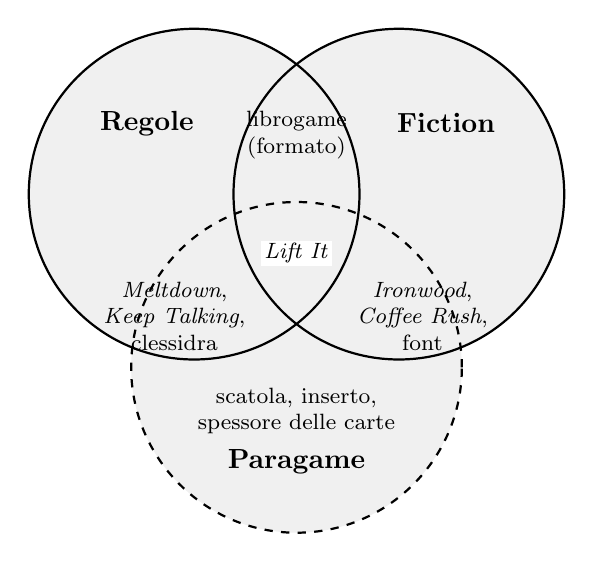
\begin{tikzpicture}[font=\small]
  \fill[gray!12] (0,0) circle (2.1cm);
  \fill[gray!12] (2.6,0) circle (2.1cm);
  \fill[gray!12] (1.3,-2.2) circle (2.1cm);
  \draw[thick] (0,0) circle (2.1cm);
  \draw[thick] (2.6,0) circle (2.1cm);
  \draw[thick, dashed] (1.3,-2.2) circle (2.1cm);
  \node[font=\bfseries] at (-0.6,0.9) {Regole};
  \node[font=\bfseries] at (3.2,0.9) {Fiction};
  \node[font=\bfseries] at (1.3,-3.4) {Paragame};
  \node[font=\footnotesize, align=center] at (1.3,0.75) {librogame\\(formato)};
  \node[font=\footnotesize, align=center] at (-0.25,-1.55)
    {\emph{Meltdown},\\\emph{Keep Talking},\\clessidra};
  \node[font=\footnotesize, align=center] at (2.9,-1.55)
    {\emph{Ironwood},\\\emph{Coffee Rush},\\font};
  \node[font=\footnotesize, align=center, fill=white, inner sep=1pt]
    at (1.3,-0.75) {\emph{Lift It}};
  \node[font=\footnotesize, align=center] at (1.3,-2.75)
    {scatola, inserto,\\spessore delle carte};
\end{tikzpicture}
\caption{Regole, fiction e paragame come tre aree con i bordi sfumati. Il paragame è
ciò che non è né regole né fiction, ma si sovrappone spesso a entrambe. La posizione
degli esempi riprende i commenti di Ruggero durante la lezione: \emph{Lift It} ``è al
centro'', \emph{Ironwood} aiuta soprattutto la fiction, \emph{Meltdown} e \emph{Keep
Talking and Nobody Explodes} soprattutto le meccaniche.}
\label{a10:fig:aree}
\end{figure}

\paragraph{Approfondimento: Genette e le ``soglie'' del testo.} Il termine
\emph{paratesto} viene dal critico francese Gérard Genette, che lo ha sistematizzato in
\emph{Soglie} (\emph{Seuils}, 1987). Per Genette il paratesto è ciò che fa di un testo
un libro e lo presenta al lettore: il titolo, il nome dell'autore, la copertina, le
dediche, le prefazioni, le note, ma anche il formato, la collana, la tipografia. È una
``soglia'' tra l'interno e l'esterno del testo, una zona di transizione che orienta la
lettura. L'idea di applicare lo stesso concetto ai giochi (paragame, paragioco) è
diffusa nei \emph{game studies}, dove il termine \emph{paratext} viene usato anche per
tutto ciò che circonda un gioco (\emph{trailer}, recensioni, guide, comunità). Nella
lezione di Ruggero il senso è più vicino a quello originale di Genette: le
caratteristiche materiali e formali dell'oggetto-gioco.

% ---------------------------------------------------------------------
\section{Le aree del paragame}
\label{a10:sec:aree}

``Su quali aspetti del paragame possiamo lavorare? E qui abbiamo l'ondata di robe.
Andiamo con calma: sono tante zone, ma sono sicuro che le vediamo tutte.'' La
tabella~\ref{a10:tab:aree} le riassume; le sezioni seguenti le vedono una per una.

\begin{table}[htbp]
\centering
\small
\begin{tabular}{@{}p{3.1cm}p{5.4cm}p{4.7cm}@{}}
\toprule
\textbf{Area} & \textbf{Domande da farsi} & \textbf{Esempi della lezione} \\
\midrule
Materialità & di che cosa sono fatti i componenti? Serve un'app? Quanto sono spesse
le carte? Clessidra o timer? & dadi di legno e di plastica; \emph{Lands of Galzyr} su
tablet e telefono; carte \emph{blue core}; \emph{standee} \\
Formato & come sono comunicati regole e testi? Che font, che dimensione, che misura
della carta? & \emph{Bureaucracy} di \emph{Magic}; il \emph{200 Word RPG} \\
Regolamento & quante pagine? Quanti libretti? Video, glossario, \emph{playthrough},
\emph{play aid}? & \emph{Irish Gauge}; \emph{Root}; riassunto delle icone \\
Scatola & dove andrà, nei negozi e a casa? & le vecchie scatole lunghe; la Kallax;
\emph{Dobro} \\
Grafica e illustrazioni & che cosa comunica l'aspetto visivo? Quante icone? &
\emph{Master of Rules}; \emph{Rolling Stock Stars}; \emph{A Feast for Odin} \\
Interfaccia analogica & com'è il \emph{wireframe}? Dove stanno le informazioni quando
il componente è in uso? & la carta di \emph{Magic}; la plancia di \emph{The
Gallerist}; le carte a ventaglio e i mancini \\
Ambiente & dove si gioca? Quanto spazio serve? Che suoni, che vibrazioni? & il tavolo
IKEA; il treno e l'aereo; \emph{Jenga} \\
Audio & serve una colonna sonora? & \emph{Escape: The Curse of the Temple} \\
Contesto & che cosa deve sapere chi gioca sul luogo e sulla cultura del gioco? &
\emph{Jakarta Traffic}; \emph{This War of Mine} \\
Lingua & il gioco dipende dalla lingua? & i giochi di Lacerda; \emph{Race for the
Galaxy}; \emph{Magic} \\
Spazio urbano e ibridi & la città, la stanza, il telefono come parte del gioco &
\emph{Pac-Manhattan}; \emph{Vroom}; \emph{World of Yoho} \\
\bottomrule
\end{tabular}
\caption{Le aree progettabili del paragame presentate a lezione, con le domande che
suggeriscono e gli esempi usati da Ruggero. Inserti e \emph{setup}, discussi alla fine
(sezione~\ref{a10:sec:inserti}), sono un'altra area della stessa famiglia.}
\label{a10:tab:aree}
\end{table}

% ---------------------------------------------------------------------
\section{Materialità}
\label{a10:sec:materialita}

La prima area è la \textbf{materialità}: ``le proprietà fisiche degli elementi di
gioco''. Legno, plastica, metallo. Prendiamo dei dadi classici di legno e dei dadi di
plastica: che cosa cambia? ``Il rimbalzo, il rumore, la sensazione al tatto.'' Sono
aspetti \textbf{cinestetici}, ``che assolutamente impattano''. Ma cambia anche altro,
``perché nel paragame spesso ci sono anche degli \textbf{aspetti culturali}''. In un
Eurogame, in un \emph{German}, si troveranno dadi di legno; in un \emph{American}, in un
\emph{dungeon crawler}, dadi di plastica. (Se n'era parlato, ``vagamente'', nella
lezione sui casi studio, a proposito dei componenti.)

\subsection{Il digitale come materiale}

Anche il \textbf{digitale} fa parte della materialità: se il gioco ha o richiede
un'app, un cellulare, un tablet, ``quello è un aspetto di materialità da considerare''.
Ruggero porta un esempio di un gioco che ha giocato, che la trascrizione chiama ``Lens
of Galsy''\footnote{Con ogni probabilità \emph{Lands of Galzyr} (Snowbright Studio,
2021), gioco d'avventura narrativo con app.}: ``molto carino, ma chiaramente pensato per
un tablet''. L'app ha tanto testo e tante cose a schermo, e sul cellulare, molto più
piccolo, ``non si vede niente''. ``L'app è la stessa, ma in base a dove lo stiamo
giocando, quel gioco può diventare un incubo di accessibilità, o qualcosa invece molto
più comodo da giocare.''

\subsection{Le carte non sono tutte uguali}

Quanto sono spesse le carte? Di che materiale sono? \emph{Blue core}, \emph{black
core}, \emph{white core}? ``Le carte non sono tutte uguali. Vi sembrano uguali perché le
usate da chi gioca, ma da produrre sono diverse.'' Quelle ``che si spaccano al volo'' si
riconoscono subito, perché sono le più economiche: di solito quelle di giochi come
\emph{Uno} o di giochi di carte ``più cheap da produrre'', in cui basta una pieghetta
per rovinare una carta ``forever and ever''. Altri giochi usano il \emph{blue core} o il
\emph{black core}; le carte di \emph{Magic}, per esempio, hanno il \emph{blue core}.

Ruggero semplifica la struttura: di solito una carta da gioco ha \textbf{tre strati},
lo strato con l'immagine sul fronte, quello con l'immagine sul retro, e in mezzo il
materiale che ne determina, tendenzialmente, la \textbf{rigidità}. ``Poi è più
complessa di così'', perché ci possono essere filigrane, texture e altro; ma la parte
centrale dice che cosa succede quando la carta si piega, o quando la si mescola male.

\paragraph{Le carte americane.} Una studentessa chiede delle carte da gioco americane,
``quelle di tela'', come le \emph{Bicycle}, che in Europa si vedono poco: c'è un motivo
per cui sono ``molto più fighe''? Sì: hanno una produzione che include \textbf{materiali
plastici} nella loro texture, che le rende più resistenti e crea un \textbf{attrito}
diverso. Sono carte che ``scivolano molto bene'' (``non ho più italiano, scusatemi''), e
infatti sono usatissime negli spettacoli di prestigiazione, perché si possono manovrare
velocemente, ``per chi le sa maneggiare; io no, di sicuro''. Le carte prodotte in Europa,
invece, hanno di solito un attrito molto più alto, e sono ``non fantastiche'' da usare
in modo ``sgaggio''.

\paragraph{Europa, America, Cina.} Lo stesso vale per i dadi: l'America fa un uso
abbondante di plastica nei giochi perché spesso produce in \textbf{Cina}, mentre
tipografie, stamperie e aziende che producono carte in Europa hanno ``molto poco
accesso'' a quei materiali. ``Quindi spesso siamo più forti nel legno e nella carta che
nella plastica.'' È ``un vaso di Pandora che a voi interessa il giusto'': per i progetti
del corso, quel tipo di finiture ``ve lo sognate, salvo pagare un bordello''. Ci sono
alcune fabbriche che possono fare cose bizzarre, nell'Est Europa e in Repubblica Ceca,
ma la maggior parte di chi produce stampa in Cina, oppure non usa quei materiali.

\paragraph{Miniature e \emph{standee}.} Stesso discorso per le miniature o gli
\textbf{\emph{standee}}, il cartoncino infilato in un piedistallo al posto della
miniatura di plastica. In un \emph{American} è facile trovare la plastica; in un gioco
prodotto e stampato in Europa, ``non trovate delle miniature di plastica'', perché non
c'è praticamente nessuna azienda europea di giochi da tavolo che possa stampare in
Europa la plastica a iniezione usata per le miniature; anche chi produce in Europa giochi
con parti di plastica le fa stampare in Cina. Per questo molti giochi europei degli anni
'90 e 2000, \emph{German} ed Eurogame, ``la plastica proprio la skippano'': se hanno
delle figure, sono \emph{standee}.

\paragraph{Approfondimento: che cosa fa davvero il ``core''.} Nella produzione di carte
da gioco lo strato centrale (\emph{core}) ha due funzioni: dà rigidità e soprattutto
rende la carta \textbf{opaca}, impedendo di vedere il fronte in controluce, cosa
essenziale in qualunque gioco con informazioni nascoste. \emph{Blue core} e
\emph{black core} sono nomi commerciali di cartoncini a più strati con un'anima
colorata scura. Sulle carte americane del tipo \emph{Bicycle}, il cartoncino è in
genere rivestito da una finitura goffrata e laccata (la cosiddetta \emph{air-cushion
finish}) che riduce l'attrito; le carte \emph{interamente} di plastica (PVC o acetato)
esistono, ma sono un prodotto diverso e più costoso.

\subsection{Clessidra o timer?}

``Occhio alla materialità, perché la materialità non va a impattare solo il paragame e
basta.'' Il classico esempio di materialità che impatta anche le \textbf{regole} è la
\textbf{clessidra}. Che differenza c'è tra un timer sul cellulare e una clessidra? Uno
studente risponde: ``la tangibilità''. Sì, e soprattutto quella che si chiama di solito
l'\textbf{informazione discreta}: con il timer si sa con precisione quando mancano un
secondo, due, tre, quattro secondi. Con la clessidra no: si vede chiaramente quando è
finita, ma ha ``quel pizzichino di incertezza che crea una tensione molto precisa che il
timer non ha''. Entrambi creano tensione, adrenalina, frenesia, ma in modo diverso; e
sapere quale dei due serve al proprio gioco ``non è così scontato''
(tabella~\ref{a10:tab:clessidra}).

\begin{table}[htbp]
\centering
\small
\begin{tabular}{@{}p{3cm}p{5cm}p{5cm}@{}}
\toprule
 & \textbf{Timer (cellulare)} & \textbf{Clessidra} \\
\midrule
Informazione & discreta e precisa: si sa quanti secondi mancano & continua e
incerta: si vede la sabbia scendere, ma non si sa con precisione quanto manca \\
Tensione & c'è, ed è ``contata'' & c'è, con ``un pizzichino di incertezza'' in più \\
Fiction & neutra, a meno di suoni scelti apposta & può essere diegetica (vedi il
fiammifero di \emph{Scandal in the Deep}, sezione~\ref{a10:sec:casi}) \\
Domanda da farsi & perché un timer e non una clessidra? & perché una clessidra e non
un timer? \\
\bottomrule
\end{tabular}
\caption{Timer e clessidra come scelta di materialità che incide sulle regole e sulla
tensione di gioco.}
\label{a10:tab:clessidra}
\end{table}

Qui Ruggero fa un annuncio che vale per il resto del corso: ``io ve lo ricordo, ve
l'avevo già accennato, ve lo ripeto: quando vedremo i \emph{pitch}, ma anche i vostri
progetti più avanti, nelle ultime lezioni, \textbf{io vi chiederò tantissimi
perché}''. Perché avete scelto una cosa, perché l'avete fatta, perché l'avete decisa.
``Se avete una clessidra e non un timer, io vi chiederò perché avete una clessidra e non
un timer. Perché avete la plastica, la carta, e così via. Voi dovete dirmi il perché
delle cose che fate.''

% ---------------------------------------------------------------------
\section{Formato}
\label{a10:sec:formato}

Il \textbf{formato} è il modo in cui sono comunicati, per esempio, regole e testi:
frasi o icone? Che font? Quanto è alto, che dimensione ha? E la carta, com'è fatta,
quanto è grande?

\paragraph{\emph{Bureaucracy}.} Il primo esempio è una carta di \emph{Magic} ``volutamente
fatta male'': \emph{Bureaucracy}, da una di quelle serie \emph{easter egg} (umoristiche)
che \emph{Magic} pubblica ogni tanto\footnote{La trascrizione aggiunge un dettaglio
sul simbolo dell'espansione che non è ricostruibile (``ha l'uomo rotto suonate come
simbolo''). \emph{Bureaucracy} appartiene alle espansioni parodiche di \emph{Magic}, le
cosiddette \emph{Un-set}.}. Per il testo è stato scelto un font piccolissimo (``mi
sembra che fosse un corpo 5, o addirittura 6''), per renderlo ``un muro di testo
oppressivo'': tematicamente coerente con il nome della carta.

\paragraph{La misura delle carte di \emph{Magic}.} Qualcuno sa quanto sono grandi le
carte di \emph{Magic}? ``Una dimensione da poker.'' In millimetri sono ``cifre
bizzarre'', perché in realtà la misura è di \textbf{3,5 per 2,5 pollici}\footnote{La
trascrizione riporta cifre storpiate (``88,4 per 69,5''). 3,5 per 2,5 pollici sono circa
88,9 per 63,5 millimetri; la misura nominale indicata di solito per le carte di
\emph{Magic} è 63 per 88 millimetri.}, ``in un sistema stupido americano di
misurazione'' (``ormai l'ho detto, è troppo tardi''). E in quella dimensione non c'è
tutto lo spazio che si vuole, perché una parte è dedicata all'\textbf{illustrazione}:
lo spazio per il testo, con il font e la dimensione scelti, è ancora più ridotto.
Questo non impatta solo il formato, ma anche le \textbf{regole}: ``una regola complessa
sarà difficile da scrivere in quello spazio'', e quindi il formato costringe a scegliere
regole che ci stiano dentro.

\paragraph{Il \emph{200 Word RPG}.} Un caso estremo: il \emph{200 Word RPG}, una sfida
in cui si scrivono giochi di ruolo completi in \textbf{200 parole}. Il paragame è il
formato stesso delle 200 parole: ``ditemi voi se non vi impatta le regole, quel
formato''.

``Non prendete questa cosa qua come del contorno, come una cosa che è un di più.
Questa roba qui vi va a impattare come voi create i giochi, e se lo sapete, potete
lavorarci attorno.''

% ---------------------------------------------------------------------
\section{Regolamento}
\label{a10:sec:regolamento}

Il \textbf{regolamento} è un'area a sé. Quante pagine ha? Una o quaranta? Che cosa
cambia? ``Se io vi dico: venite, c'è un party game, e tiro fuori un manuale da 60
pagine, che cosa succede?'' Succede che nessuno lo gioca.

\paragraph{\emph{Irish Gauge}: un caso positivo.} All'opposto, un caso ``incredibile'':
\emph{Irish Gauge}\footnote{La trascrizione dice ``Irish Gouge'' e attribuisce il gioco a
``Amable Holland'', più avanti ``Anne Blowland''. È \emph{Irish Gauge}, gioco
ferroviario di Amabel Holland.}, un gioco economico ferroviario ``bellissimo'', di circa
un'ora di partita, in cui si comprano azioni e si costruiscono ferrovie, con una
complessità significativa sul tavolo, ``un gioco comunque bello intenso''. E il
regolamento è \textbf{un singolo foglio di carta} ``che lascia zero dubbi dopo che lo si
è letto''. ``Bellissimo, irraggiungibile forse.'' È una sorpresa positiva; il caso
contrario (il party game da 60 pagine) è una sorpresa negativa che uccide il gioco.

\paragraph{QR code e video.} Chi gioca spesso avrà notato che sempre più regolamenti
hanno un \textbf{QR code} o un link a un video in cui le regole vengono spiegate.
Perché? ``Non sappiamo più leggere'' è ``la versione più nichilista''. La risposta ``più
banale e meno nichilista'' è che \textbf{le persone imparano in modi diversi}: un
regolamento scritto in un certo modo può andare benone per una persona ed essere un
disastro per un'altra.

\paragraph{Più libretti per lo stesso gioco.} Alcuni giochi hanno più di un libretto di
regole. \emph{Root}, per esempio, ha la \textbf{guida rapida} (il \emph{learn to play}),
scritta come un regolamento da leggere al tavolo, e la \textbf{Legge di Root}, scritta
come un \textbf{manuale tecnico}: paragrafi 1.1.1, 1.1.2, 1.1.3, 1.2.1 e così via, con
glossario. ``Il gioco è lo stesso. Lo si impara a giocare in entrambi i modi, ma parlano
a due persone completamente diverse.''

\paragraph{I costi.} Ogni scelta ha un costo. Un regolamento in più costa la
produzione di un regolamento in più, \textbf{a ogni copia} stampata. Il video è un costo
diverso: lo si paga una volta, all'inizio, lo si mette online ``e quel video lì è lì''.
``Se tu stampi 100 copie o ne stampi 10.000, il video non ti costa di più. Il
regolamento sì.''

\paragraph{Glossario, \emph{playthrough}, \emph{play aid}.} Altre domande: c'è un
\textbf{glossario}? Un \emph{playthrough}? Un \emph{play aid}? E le icone, dove sono
riassunte? Dove si trova di solito il riassunto delle icone? Due risposte, ``entrambe
vere''. Tancredi: \textbf{nell'ultima pagina del regolamento}, usata spesso proprio per
questo, perché si può tenere il regolamento girato sul tavolo e avere il riassunto
davanti. Tiziana: in un \textbf{\emph{play aid}}, un cartoncino, magari uno a persona,
con il riassunto delle icone. Quando l'uno e quando l'altro? Dipende da \textbf{quante
icone} ha il gioco. In \emph{Race for the Galaxy} un riassunto a testa non esiste,
``perché il riassunto delle icone di \emph{Race for the Galaxy} è così'' (e Ruggero
mostra quanto è lungo). In giochi con cinque, sei, una decina di icone è facile avere
una carta personale che le riassume, magari con il \textbf{flusso del turno} sul retro.

\paragraph{Il \emph{playthrough} e l'\emph{actual play}.} Più avanti, su richiesta di
uno studente (``Ruggero, non so se l'hai detto: il \emph{playthrough}?''), Ruggero torna
sul punto. Il \textbf{\emph{playthrough}} è \textbf{una giocata descritta}. Molti giochi
lo fanno spezzandolo in esempi: i classici esempi in cui ``Tizio e Caio fanno A, B, C,
poi Tizio fa B e Caio piange perché ha perso la partita''. Questi esempi non sono solo
un'applicazione delle regole: sono una descrizione di \textbf{che cosa fanno le persone
al tavolo}. Alcuni giochi, soprattutto di ruolo, includono il cosiddetto \textbf{\emph{actual
play}}: un'intera partita descritta, alternando le parti di \emph{roleplay} e quelle
meccaniche (``Tizio tira e fa 18, quindi apre questa cosa; poi Caio dice questa cosa con
il suo personaggio''). Dove si trovano\footnote{La trascrizione attribuisce la domanda a
qualcuno che si rivolge a ``Pietro''; con ogni probabilità è un errore di trascrizione
per ``Ruggero''.}? Sono ``comunissimi nei giochi di ruolo'': molti giochi di ruolo
contemporanei hanno esempi di \emph{actual play}, di solito in fondo al manuale. Gli
esempi sparsi nei regolamenti sono ``un'estrazione del \emph{playthrough}'', scritti con
la stessa idea; il \emph{playthrough} vero e proprio è l'esempio di partita completa. Nei
giochi da tavolo più commerciali è raro, ``perché le pagine dei regolamenti costano'', e
una partita completa prende molto spazio. Rientra quindi soprattutto nei giochi di
ruolo, che hanno già manuali da cento pagine e passa e non hanno il problema di stare
sotto le 16 pagine, ``perché sennò la gente si spaventa'' davanti a un regolamento da
20.

% ---------------------------------------------------------------------
\section{La scatola}
\label{a10:sec:scatola}

Nel formato rientra anche la \textbf{scatola}. Ruggero è convinto di averne già parlato
(``non abbiamo mai parlato delle scatole? Secondo me no'') e la affronta con una
domanda: come erano fatte le scatole del vecchio \emph{Risiko!} o del vecchio
\emph{Monopoly}? ``Basse e lunghe.'' Perché? ``Ci stava il tabellone''; ``si impilavano''.
La domanda, precisa Ruggero, non è che cosa c'era dentro, ma \textbf{dove doveva andare}
la scatola: nei negozi di giocattoli e, a casa, dove venivano messi i giochi trenta,
quarant'anni fa? Non nella libreria: \textbf{negli armadi}. ``Non era una questione
estetica'': l'armadio è stretto e lungo, e la scatola doveva entrare lì.

E oggi, dove vanno messi? In libreria. Quale libreria? La \textbf{Kallax}\footnote{La
trascrizione dice ``Callax'' e, a tratti, ``Galaxy''.} dell'IKEA, ``la libreria più
venduta del mondo''. Com'è fatta? ``\textbf{A cubi}.'' La scatola del vecchio
\emph{Monopoly} lì dentro non entra (``puoi metterla in cima, certo''). Ma se oggi un
editore vuole che il suo gioco entri ``nella libreria più venduta del mondo'', il gioco
deve entrare in un cubo. ``È tutto qui. \textbf{Una scelta dell'IKEA ha deciso che le
nostre scatole ora sono quadrate}.'' L'IKEA non ha convinto gli editori di niente: ``è
una roba che viene naturale, perché tutta l'umanità è intrecciata. Le decisioni che
prende qualcuno vanno a impattare qualcun altro''. Chi vuole che il proprio gioco sia in
vista in libreria deve fare i conti con il cubo.

Ruggero si concede qui una raccomandazione generale: ``se c'è una cosa che voglio che vi
portiate via da questo corso, una cosa'' (``poi, se fate anche giochi dopo, belli,
benissimo''), ``la cosa migliore per me, perché sono contento, ho fatto il mio lavoro,
posso morire in pace'', è questa: \textbf{ragionate quando fate le cose}. ``Potete
ragionare sulle cose quanto volete. Più ci ragionate, più avete aree operative su cui
fare le cose.''

\paragraph{Approfondimento: il ``formato Kallax''.} Il vano interno di una Kallax misura
circa 33 per 33 centimetri, per una profondità di poco inferiore ai 39. Non a caso un
gran numero di giochi da tavolo contemporanei di formato ``standard'' ha una scatola
quadrata di circa 30 centimetri di lato: è il formato che sta in un vano in piedi o
coricato, e che si impila bene. Molti editori lo indicano ormai esplicitamente tra i
vincoli di progettazione della scatola, insieme al peso e ai costi di spedizione.

% ---------------------------------------------------------------------
\section{Grafica e illustrazioni}
\label{a10:sec:grafica}

``\textbf{Graphic design e illustrazioni sono due cose diverse}. Non confondete le
cose.'' Le \textbf{illustrazioni} sono tendenzialmente l'\emph{art}: le immagini,
gli sfondi, i personaggi, i luoghi, la parte di \emph{world building}. Il
\textbf{graphic design} sono le icone, la UX. ``Non fate fare queste due cose alla
stessa persona, sennò di solito viene una porcheria.''

\subsection{Due edizioni, due destini}

Sulla slide ci sono due scatole: una con un omino che tiene sopra di sé delle forme, e
una con un'auto sotto un cielo stellato, una notte al neon. ``Sono lo stesso gioco'':
\emph{Master of Rules}\footnote{Il titolo è quello della trascrizione e non è stato
possibile verificarlo.}, ``un gioco bellissimo'', che nella sua edizione americana è
uscito con la prima scatola. ``Vi sorprenderà sapere che in America non è andato per
niente, nonostante sia un gioco incredibile. Qualcuno ha un'idea del perché?'' Le
risposte sono impietose: ``fa schifo'', ``sembra quelli che trovi in edicola''. E
dentro, dice Ruggero, ``è ancora più brutto''.

Uno studente lo provoca: ``io ho dei giochi che hanno copertine orrende da 100 euro'':
gli \textbf{Splotter}\footnote{Splotter Spellen, editore olandese noto per giochi
molto pesanti e per una grafica spartana.}. Ruggero non lo nega, ma ribalta la
domanda: la grafica degli Splotter ``è comprensibile perché la fanno così, ovvero perché
non gliene frega niente''; ma ``sarebbero giochi peggiori con una grafica migliore?'' ``La
risposta, nel tuo cuore, la sai: no.'' Le immagini danno un'esperienza, un \emph{look
and feel}.

Tiziana porta un caso concreto: un amico ha comprato \emph{Darwin's Journey}\footnote{
La trascrizione dice ``Darvis Journey''.}, ``un gioco che secondo me è bellissimo'', e
l'ha rivenduto, perché l'impatto grafico per lui è stato terribile: ``colori scuri sul
marrone''. ``Non riusciva a vederlo.''

Ruggero avrebbe potuto fare ``mille altri esempi'' di giochi usciti in due edizioni con
grafiche diverse, ``una che va a picco e non la vedete più, e l'altra che invece diventa
roba di culto''. Perché la grafica ha un impatto ``non solamente in termini di
leggibilità, ma anche di \emph{vibes}''. Lui, personalmente, non ci fa caso: ``io mi
gioco anche \emph{Rolling Stock Stars}'', che ``sembra fatto da marito e moglie su
Excel''. Ma altre persone vedono quella grafica e dicono ``non giochiamo a \emph{Rolling
Stock Stars}''. E finisce che ``il piccolo Ruggero'' lo gioca ``una volta ogni cinque
anni, perché nessuno vuole giocarci''. La conclusione: ``un gioco può beneficiare
dall'essere \textbf{non visivamente ostile} alle persone che lo vogliono giocare''.
Un altro studente aggiunge, a proposito di grafiche difficili, \emph{Terraforming
Mars} (``la carta con il cane''), e Ruggero si arrende: ``volete farmi stare male
oggi''.

\subsection{Il font, e quante icone}

Anche il \textbf{font} rientra nella grafica, non solo nel formato: il font del titolo,
il font dei contenuti. Ruggero cita un gioco che ha venduto ``proprio per il font che
aveva'', e promette di mostrarlo dopo, perché ``ci vuole del tempo per elaborare''
(lo farà nella discussione finale: è \emph{Al Rashid}, sezione~\ref{a10:sec:alrashid}).

Ultimo punto della grafica: \textbf{quante e quali icone} avete? Sulla slide c'è \emph{A
Feast for Odin}\footnote{La trascrizione dice ``Fist for Odin''. \emph{A Feast for
Odin} (Uwe Rosenberg, 2016).}: ``quel gioco lì ha 50 azioni diverse. Non devo dirvi
altro''. Ragionate sulle icone che avete.

\paragraph{L'intervento di Tiziana.} Tiziana porta un esempio di segno opposto: ha
giocato di recente a un gioco che la trascrizione chiama ``MNFR''\footnote{Il titolo
non è ricostruibile dalla trascrizione.}, abbastanza complesso, con varie tipologie di
azioni e una serie di cose che si succedono; ma le icone ``sono sempre quelle'', in
numero limitato, e una volta capite ``te le ritrovi in tutte le salse, nelle varie parti
e sezioni del gioco''. ``E questo aiuta molto.'' Ruggero concorda e cita di nuovo
\emph{The Gallerist} (``bellissimo, un capolavoro''): sono giochi in cui, se si fa un
buon lavoro sulle icone, il gioco ``non ti chiederà mai di andare a leggere il
regolamento durante la partita''. Lui ha giocato di recente un Eurogame di designer
giapponesi\footnote{La trascrizione dice ``Elder Tide degli stessi di Gisoji''; titolo
e autori non sono ricostruibili con sicurezza.}, con un \emph{setting} un po' fantasy, in
cui si costruiscono edifici su un'isola e ci si muove di porto in porto per vendere
risorse: ``ha tante icone, ma dopo i primi cinque minuti, per tutte le altre due ore
della partita, non abbiamo guardato il regolamento una singola volta, perché è tutto
chiaro, tutto immediato''. Si torna ai pilastri: immediatezza, efficienza,
memorabilità.

% ---------------------------------------------------------------------
\section{Interfaccia analogica}
\label{a10:sec:interfaccia}

La voce successiva è l'\textbf{interfaccia analogica}: ``si parla di
\emph{wireframing}, di solito''. È la struttura nuda della carta, quelle linee che, in
stampa, ``verranno abbellite da frame, cornici''. Ma il \emph{wireframe} è quello. ``Se
vi chiedo di disegnarmi a occhi chiusi su un foglio una carta di \emph{Magic}, voi sapete
come disegnarmela'': divisa a metà, al centro un rettangolino molto sottile, un
rettangolo più grosso in alto, uno più grosso in basso. ``Quella parte lì è una parte su
cui potete ragionare.''

\subsection{La scatola in piedi: \emph{Dobro}}

Anche la grafica della scatola è interfaccia. ``Se io prendo la scatola e la metto in
verticale, posso leggere il titolo?'' C'è una ``diatriba'' che Ruggero non apre
(``siete ancora persone sane di mente, non voglio rovinarvi la vita''): i giochi da
tavolo si mettono in libreria in verticale o in orizzontale? Lui fa un mix, ma molte
persone li mettono in verticale, e molte scatole non hanno il nome del gioco su tutti i
lati: alcune lo hanno solo per il lungo, e in verticale il nome è storto. L'esempio
positivo è \emph{Dobro}, di cui il suo gruppo ha rifatto la scatola per l'edizione
italiana: un lato lungo con il nome in orizzontale, il lato opposto con il nome in
verticale, e lo stesso sui due lati corti. ``Non importa come la mettete: un modo per
trovarla con il nome che si vede da fuori lo trovate sicuramente.'' Mentre ``ho delle
scatole in cui non si vede il nome, perché purtroppo non l'hanno messo su tutti i
lati''. Quindi: \textbf{la grafica della scatola non va lasciata al caso}, ``perché è
funzionale''. (``Mi sto arrabbiando, si vede, perché questa cosa mi fomenta.
Purtroppo per voi.'')

\subsection{Le opere sulla plancia di \emph{The Gallerist}}

Una studentessa chiede di chiarire: l'interfaccia analogica è il discorso della scatola
e della visibilità, o altro? Ruggero torna al \emph{wireframe}, ``cioè a come sono fatte
le carte'', e porta l'esempio di \emph{The Gallerist}: si acquistano opere d'arte da
esporre nella propria galleria, e la \textbf{plancia} personale raffigura la galleria.
Le tre tessere delle opere esposte si sovrappongono perfettamente ai \textbf{muri
disegnati sulla plancia}, ``andando letteralmente a mettere le opere in vista nella
nostra galleria''. Non è casuale: hanno pensato la grafica in modo che aiutasse a capire
che cos'è quel componente, e in modo che fosse anche soddisfacente. Di nuovo:
soddisfazione, efficienza, memorabilità, immediatezza.

\subsection{Dove stanno le informazioni quando le carte sono in mano}

Un altro aspetto dell'interfaccia è \textbf{dove si piazzano le informazioni}. Con le
carte da poker in mano, dove sono le icone? \textbf{In alto a sinistra}: quando le carte
sono aperte a ventaglio, ciascuna copre buona parte di quella precedente, e l'angolo in
alto a sinistra è ``la cosa più visibile'' (figura~\ref{a10:fig:ventaglio}).

Tancredi apre una parentesi sui \textbf{mancini}: ``io da mancino, tutte le volte che
apro le carte da poker, non vedo assolutamente niente''. Ruggero conferma (``ho degli
amici mancini, e se avete un gioco che non pensa ai mancini lo sapete al volo, perché
ve lo dicono''), e lo riconduce all'\textbf{accessibilità}: i mancini tengono in mano le
carte come tutti, ``è solo che per natura il ventaglio lo fanno nell'altro verso''. Molti
giochi per questo \textbf{duplicano} il seme della carta, mettendolo anche in alto a
destra. In alcuni giochi è più complicato: quando l'angolo in alto a sinistra ospita
icone meccaniche, come il costo, come in \emph{Race for the Galaxy} (``è il problema
minore di questa carta, mi sento di dire''), duplicare vuol dire affollare ancora di più
una carta già piena. ``Volete davvero duplicare le informazioni di questa carta
dall'altro lato? Io non lo farei.'' Non sempre si può; ma ``è assolutamente una
considerazione da fare''.

\begin{figure}[htbp]
\centering
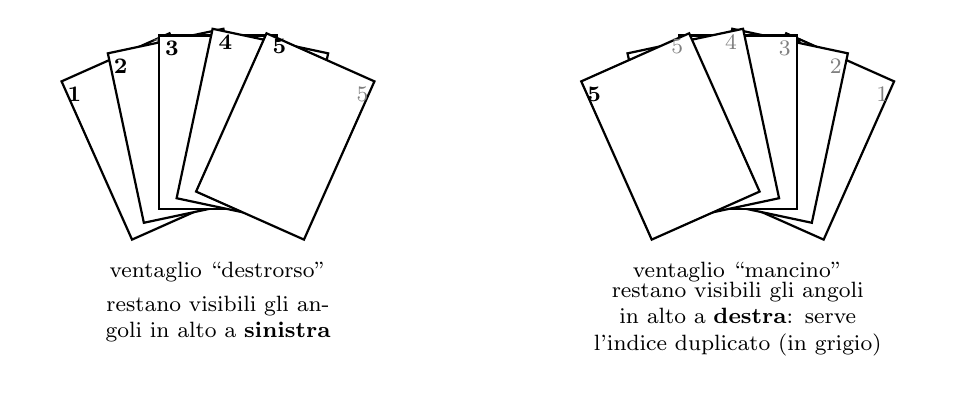
\begin{tikzpicture}[font=\footnotesize]
  % mano destrorsa: ventaglio verso destra
  \begin{scope}[shift={(0,0)}]
    \foreach \a/\i in {24/1, 12/2, 0/3, -12/4, -24/5}{
      \begin{scope}[rotate around={\a:(0,-2.6)}]
        \draw[thick, fill=white] (-0.75,-1.6) rectangle (0.75,0.6);
        \node[anchor=north west, inner sep=2pt] at (-0.75,0.6) {\textbf{\i}};
        \node[anchor=north east, inner sep=2pt, text=gray] at (0.75,0.6) {\i};
      \end{scope}
    }
    \node at (0,-2.4) {ventaglio ``destrorso''};
    \node[text width=4.6cm, align=center] at (0,-3.0)
      {restano visibili gli angoli in alto a \textbf{sinistra}};
  \end{scope}
  % mano mancina: ventaglio nell'altro verso
  \begin{scope}[shift={(6.6,0)}]
    \foreach \a/\i in {-24/1, -12/2, 0/3, 12/4, 24/5}{
      \begin{scope}[rotate around={\a:(0,-2.6)}]
        \draw[thick, fill=white] (-0.75,-1.6) rectangle (0.75,0.6);
        \node[anchor=north west, inner sep=2pt] at (-0.75,0.6) {\textbf{\i}};
        \node[anchor=north east, inner sep=2pt, text=gray] at (0.75,0.6) {\i};
      \end{scope}
    }
    \node at (0,-2.4) {ventaglio ``mancino''};
    \node[text width=4.6cm, align=center] at (0,-3.0)
      {restano visibili gli angoli in alto a \textbf{destra}: serve l'indice
      duplicato (in grigio)};
  \end{scope}
\end{tikzpicture}
\caption{Le carte a ventaglio. L'informazione più importante va nell'angolo che resta
scoperto; chi apre il ventaglio nell'altro verso, come molti mancini, vede l'angolo
opposto, e per questo molti giochi duplicano il seme o l'indice in alto a destra.
Schema illustrativo: l'ordine con cui le carte si sovrappongono dipende da come le si
apre.}
\label{a10:fig:ventaglio}
\end{figure}

Ruggero annuncia che su grafica e formato c'è ``un'altra cosa'', da riprendere dopo (lo
farà con gli inserti, sezione~\ref{a10:sec:inserti}).

% ---------------------------------------------------------------------
\section{Ambiente}
\label{a10:sec:ambiente}

\textbf{Dove} giocheranno le persone al vostro gioco? Su un tavolo, a letto, per terra,
in piedi? E \textbf{quanto spazio} prende il gioco? Qualcuno sa quanto spazio, al
massimo, deve prendere un gioco da tavolo \emph{family} per quattro persone? ``La sapete
nel vostro cuore, la risposta.'' Gianmarco: ``\textbf{il tavolo IKEA}''. ``Bravissimo,
Gianmarco, è sempre quello.'' Il tavolo IKEA più venduto: cercate quanti centimetri
misura. ``Se il vostro gioco non entra in quel tavolo, avete un grosso problema.''

E se è un \textbf{party game}? Allora deve stare nel \textbf{tavolino da caffè}
dell'IKEA, più piccolo, quello da divano, ``per un altro tipo di ambiente''. Se è un
gioco \emph{pocket}, portatile, deve stare nei tavolini da caffè, in quelli del
\textbf{treno}, in quelli dell'\textbf{aereo}. ``Quanto spazio prende il vostro gioco
apparecchiato non è casuale. Non lasciate al caso quella roba'', altrimenti succede,
come è capitato di vedere a Ruggero, di avere ``giochi in solitaria che prendono un
tavolo per sei persone''.

Il mezzo di trasporto ha poi un altro problema: il treno e l'aereo \textbf{si muovono}.
Il gioco può starci come spazio, ma i componenti? Uno studente ricorda le
\textbf{versioni magnetiche} di scacchi e dama, e una versione mini di \emph{Azul} con
le tessere che si incastrano. E Ruggero aggiunge: \emph{Jenga} ci sta, come spazio, nel
tavolino di un aereo. Perché nessuno ci gioca in aereo? ``Per le vibrazioni dovute al
movimento.'' Appunto: ``l'ambiente non è solo spazio. L'ambiente è anche suoni, è anche
vibrazioni, è un sacco di altre cose''.

\paragraph{Approfondimento: misurare il tavolo.} Le misure dei tavoli più diffusi
nelle case cambiano da modello a modello, ma un tavolo da cucina per quattro persone ha
spesso un piano tra gli 80 per 80 e i 120 per 75 centimetri, e un tavolino da caffè è
molto più piccolo (spesso intorno ai 90 per 55 centimetri). Il consiglio di Ruggero va
preso alla lettera: misurare il piano reale di riferimento e fare un \emph{mock-up} del
gioco apparecchiato a grandezza naturale, lasciando spazio per le mani, i bicchieri, le
plance personali e i mazzi degli scarti. È uno dei test più economici che si possano
fare con un prototipo.

% ---------------------------------------------------------------------
\section{Audio}
\label{a10:sec:audio}

Altra area progettabile: l'\textbf{audio}. Serve la musica nel vostro gioco? Alcuni
giochi usano una \textbf{colonna sonora} per dare il tempo. L'esempio è \emph{Escape:
The Curse of the Temple}\footnote{La trascrizione inciampa più volte sul titolo, e
Ruggero stesso si corregge (``scusatemi, perché in tedesco\dots''). Il gioco è
\emph{Escape: The Curse of the Temple} (Kristian Amundsen \O{}stby, Queen Games, 2012).}: un
gioco in tempo reale in cui bisogna uscire dal tempio entro la durata della colonna
sonora, ``sennò siete fritti''. E a intervalli la colonna sonora fa sentire dei
\textbf{colpi di gong} che attivano eventi meccanici nel gioco. Quindi la colonna
sonora non è ``solamente un timer, una grossa clessidra'': è un \textbf{elemento
meccanico} che, con l'audio, fa altre cose. E fa anche \textbf{fiction}: dà elementi di
\emph{world building}, certe \emph{vibes}. ``È chiaro che \emph{Escape} è molto Indiana
Jones: non avete una colonna sonora techno IDM a palla.''

% ---------------------------------------------------------------------
\section{Contesto}
\label{a10:sec:contesto}

``Al \textbf{contesto} non ci pensa quasi mai nessuno, ma è molto importante'', perché
informa il gioco, ``non solo in termini di \emph{world building}, ma anche in termini di
che cosa vuole che voi facciate''.

\paragraph{\emph{Jakarta Traffic}.} \emph{Jakarta Traffic}\footnote{Titolo come nella
trascrizione.} è un gioco sul traffico di Giacarta, ``che è molto ostile'': si naviga il
traffico per fare delle consegne, e molti elementi del gioco sono \textbf{culturali}.
Spiegare le meccaniche a chi non sa come è fatta Giacarta, culturalmente, rende il gioco
molto più complesso di quanto dovrebbe essere. Qui, secondo Ruggero, hanno fatto un
buon lavoro: il manuale aiuta a capire il contesto, e hanno perfino creato una colonna
sonora usando il traffico di Giacarta come \emph{sample}, per creare un certo
\emph{mood}.

\paragraph{\emph{This War of Mine}.} Ma il contesto non è solo \emph{setting}: può
anche \textbf{informare le scelte}. Qualcuno conosce il gioco da tavolo di \emph{This War
of Mine}\footnote{La trascrizione dice ``Diceworld Mine''.}? Qual è il suo contesto?
``È una guerra, ma non mi ricordo se è una guerra vera.'' ``È a metà'': non è scritto
apertamente, ma è palesemente l'\textbf{assedio di Sarajevo}. E soprattutto, non si
giocano militari: si giocano \textbf{civili}. Se ci si approccia al gioco ``con tutto il
bagaglio culturale dei giochi di guerra'', ci si aspettano cose che il gioco non può
dare, perché ``non è un gioco di soldati in guerra: è un gioco in cui c'è la guerra, ma
non è un gioco di guerra''. Queste cose si risolvono con un mix: in parte con testo,
\emph{flavor} e \emph{world building}, in parte con il paragame, con i materiali.

% ---------------------------------------------------------------------
\section{Lingua}
\label{a10:sec:lingua}

Anche la \textbf{lingua} è un componente. Alcuni giochi sono \textbf{indipendenti dalla
lingua}: in un gioco di Lacerda\footnote{Vital Lacerda, autore portoghese di Eurogame
pesanti, tra cui \emph{The Gallerist}.}, o nella maggior parte dei \emph{German}, sulle
carte non c'è testo, ``alla buon'icona''. Lo stesso \emph{Race for the Galaxy}, lasciando
stare il nome e l'effetto ricopiato sotto, si può giocare anche senza leggere l'inglese:
``mi basta sapere che cosa fanno quelle icone''. Così \emph{The Gallerist}, o \emph{Master
of Rules}. Altri giochi no: \emph{Magic} è molto difficile da giocare se le carte non sono
nella propria lingua.

% ---------------------------------------------------------------------
\section{La città, la stanza, il telefono}
\label{a10:sec:pervasivo}

``In quali altri modi posso impattare l'esperienza di chi gioca senza passare per le
regole e per la fiction?'' Sulla slide c'è un'immagine di
\textbf{\emph{Pac-Manhattan}}\footnote{La trascrizione dice ``Pac-Man Hatton''.
\emph{Pac-Manhattan} (2004) è un gioco urbano nato alla New York University, in cui
persone vere interpretavano Pac-Man e i fantasmi nelle strade di Manhattan.}: la città,
gli aspetti \textbf{pervasivi urbani} sono anch'essi paragame.

\paragraph{La stanza come pista.} Un altro esempio è un gioco di corsa cooperativo che
la trascrizione chiama ``Vroom''\footnote{Il titolo non è stato possibile verificarlo.}:
usa il \textbf{tavolo} come spazio di gioco e chiede di prendere degli \textbf{oggetti
della propria stanza} e metterli sul tavolo come ostacoli, ``fisicamente, proprio''.

\paragraph{\emph{World of Yoho}.} Infine \emph{World of Yoho}\footnote{La trascrizione
dice ``World of Yacht'', ``World of YOHO'', ``Word of Yoko''.}, un gioco di pirati che
chiede di usare il \textbf{cellulare} su un tabellone gigantesco. Il telefono è la
propria \textbf{nave}: quando lo si sposta, sullo schermo si muove la mappa, e le parti
di quella casella di mare diventano interagibili in digitale. ``Si poteva fare senza
cellulare? Sì, con un libro degli eventi gigantesco, una seccatura infinita. Mentre così
è una cosa immediata, che si spiega in tre minuti.'' Uno studente chiede se si giochi su
un tabellone normale: sì, il gioco arriva in scatola con il suo tabellone, che si mette
sul tavolo, e chiede semplicemente di usare il telefono come nave per tutta la partita.
Ogni persona usa il proprio telefono; e nelle battaglie navali ``vedi i proiettili che
vengono sparati da una nave, che vanno sul bordo del telefono ed entrano nell'altro.
Pazzi completi. Bellissimo''.

\medskip
Prima dei casi studio, una seconda pausa: ``sono le 57'', e Ruggero dà otto minuti
``per il numero tondo'': si riprende alle 19:05.

% ---------------------------------------------------------------------
\section{Casi studio}
\label{a10:sec:casi}

``Andiamo avanti nell'ultima parte'': i \textbf{casi studio}, per vedere ``come
applichiamo le cose che abbiamo appena visto a giochi particolari''. Ce ne sarebbero
``a tonnellate''; Ruggero ne ha scelti un gruppo ``che va da giochi più regolari a cose
più \emph{deranged}, come spesso succede'', e per ciascuno dovrebbe essere chiaro perché
è stato scelto. La tabella~\ref{a10:tab:casi} li riassume.

\begin{table}[htbp]
\centering
\small
\begin{tabular}{@{}p{3.3cm}p{5.3cm}p{4.6cm}@{}}
\toprule
\textbf{Gioco} & \textbf{Elemento di paragame} & \textbf{Che cosa tocca} \\
\midrule
\emph{Cuba Libre} & due regolamenti, due diagrammi di flusso per i bot, quattro
brochure di fazione & regole, accessibilità di un gioco pesante \\
\emph{193 Days} & solo un mazzo di carte, niente regolamento & si impara giocando \\
gioco ``a metropolitana'' & creazione del personaggio piegata come una mappa turistica
& fiction, \emph{world building} \\
\emph{Shenzhen I/O} & un manuale fisico da stampare, il faldone della collector's &
meccaniche (le schede tecniche), fiction, ``feeling'' \\
pinball in scatola & dadi da schicchera su una ``scalinata'' con i flipper & meccaniche \\
\emph{Lift It} & la gru da mettersi in testa & ``al centro'' di regole, fiction e
paragame \\
\emph{Coffee Rush} & tazzine di plastica e ingredienti a forma di ingrediente & fiction,
\emph{vibes} \\
\emph{Ironwood} & una fazione tutta di legno, una tutta di metallo & fiction,
riconoscibilità, \emph{vibes} delle fazioni \\
\emph{Nyctophobia} & occhiali oscuranti per chi scappa & meccaniche, accessibilità,
fiction \\
\emph{Keep Talking and Nobody Explodes} & visore VR da una parte, manuale di carta
dall'altra & meccaniche, comunicazione \\
\emph{City of Six Moons} & nessun regolamento: un artefatto ``alieno'' & il gioco stesso
è dedurre le regole \\
\emph{Scandal in the Deep} & un fiammifero acceso come torcia & tempo reale, fiction
diegetica \\
\emph{Metal} & componenti di metalli diversi & meccaniche di destrezza (peso, massa) \\
\emph{Meltdown} & tessere di ghiaccio che si sciolgono & tema e meccaniche, inseparabili
\\
\bottomrule
\end{tabular}
\caption{I casi studio della lezione, in ordine di presentazione, con l'elemento di
paragame che li rende interessanti e l'area con cui si intreccia.}
\label{a10:tab:casi}
\end{table}

\subsection{\emph{Cuba Libre}: sei brochure}

Si parte da un gioco che Ruggero ama: \textbf{\emph{Cuba Libre}} della GMT\footnote{
\emph{Cuba Libre} (Jeff Grossman e Volko Ruhnke, GMT Games, 2013), secondo titolo della
serie COIN (\emph{COunter-INsurgency}).}, uno strategico per quattro persone, da tre o
quattro ore, sulla rivoluzione cubana. Ha tanto materiale cartaceo, inclusi dei
\textbf{diagrammi di flusso}, ``che è la cosa che tendenzialmente può intimorire le
persone''.

In alto, \textbf{due manuali}: \emph{Playbook} e \emph{Rules of Play}. Perché due?
Nessuno ha giocato \emph{Cuba Libre}, ma la classe sa già rispondere: ``forse uno ha più
le regole, l'altro lo sviluppo del gioco''. Esatto. Il \emph{Playbook} accompagna la
partita dal \emph{setup} al turno di gioco, ``scritto come un manuale di gioco da
tavolo''; le \emph{Rules of Play} sono il manuale tecnico visto con \emph{Root}: un
manuale ``con font di corpo 6-7, diviso in paragrafi, con il glossario tecnico alla
fine'', in cui, con un dubbio sul combattimento, si va alla sezione del combattimento e
si è sicuri di trovare il sottoparagrafo che interessa.

Sotto ci sono \textbf{sei ``foglioni''}: A4, ma fronte e retro e piegati a brochure,
``come se avessimo quattro facciate''. Che cosa sono? I due a destra sono
\textbf{diagrammi di flusso}, uguali, con la scritta \emph{Non-Player}: servono quando si
gioca in \textbf{solitario}, o quando si vuole riempire una delle quattro fazioni. È un
gioco a quattro fazioni asimmetriche che ha senso giocare con tutte e quattro: ``ma se
siamo in tre, o in due, che cosa facciamo? Non giochiamo a \emph{Cuba Libre}?'' I
diagrammi simulano nel dettaglio il comportamento di questi \textbf{bot}, ``un'intelligenza
artificiale analogica'', ``nel senso vecchio del termine, non generativa: macchine a
stati''. E il testo scritto è notoriamente un mezzo \textbf{lineare}, che si applica poco
alle macchine a stati; i diagrammi di flusso risolvono questo problema. Già dalla scelta
dello strumento si capisce lo scopo: rendere ``il più veloce e scorrevole possibile la
gestione di automatismi'' delle fazioni giocate dal gioco, ``senza farle troppo
stupide''.

Gli altri quattro sono \textbf{brochure uguali}, fronte e retro: quattro facciate, una per
\textbf{ogni fazione}. A che cosa servono, e perché tutti ne hanno una? Una studentessa:
riassumono le regole specifiche e asimmetriche di ogni fazione, ``e devo sapere che cosa
possono fare gli altri perché possono influire sul mio gioco''. Esatto: in uno
strategico di \emph{counterinsurgency} (``si fanno imboscate, ci si ammazza, ci si
rapisce'') bisogna sapere che cosa può fare l'avversario per impedirgli di fare ``quelle
cose brutte che vuole farmi''. E per farlo bisogna avere accesso alle stesse
informazioni che ha lui: nel ``brochurone'' c'è la propria fazione riassunta, e le altre
tre. ``È chiaro che questa cosa ha senso in un gioco strategico di questo peso, di questo
publisher. Non metterei un brochurone così dentro \emph{Risiko!}'', perché si
alienerebbe il \emph{target}.

\paragraph{Approfondimento: il diagramma di flusso come interfaccia.} L'osservazione
sui diagrammi di flusso vale anche per i progetti del corso. Un automa (un \emph{bot}, un
avversario controllato dal gioco, un evento che reagisce allo stato del tavolo) è per
natura una \emph{macchina a stati}: in base alla situazione, sceglie un ramo. Descriverlo
in prosa costringe chi legge a ricostruire mentalmente i rami; un diagramma li mostra
tutti insieme e permette di seguirne uno solo. È lo stesso motivo per cui i diagrammi
di flusso sono lo strumento standard per documentare la logica di un gioco, analogico o
digitale.

\subsection{\emph{193 Days}: solo un mazzo di carte}

All'estremo opposto del peso c'è \textbf{\emph{193 Days}}\footnote{Titolo come nella
trascrizione.}, un \textbf{gioco di ruolo per due persone}, senza \emph{master}. I suoi
componenti sono, tutti, un \textbf{mazzo di carte}: nessun libretto, nessun manuale,
nessun QR code, nessun link. ``Quando apro la scatola c'è letteralmente solo un mazzo di
carte.'' Come si impara a giocare? Lorenzo e Tiziana ci arrivano: ``si impara giocando'';
``come negli \emph{escape} in scatola: la prima carta ti dice come sistemare le altre''.
Ruggero lo mostra in camera (``ce l'ho qua dietro''): la prima carta spiega che cos'è il
gioco e che cosa fare con il resto, cioè separare due mazzetti, blu e viola, e darne uno
a ciascuna persona; poi ognuno rivela la carta \emph{start}, che spiega come leggere le
altre. ``Il gioco ti dice passo passo che cosa devi fare.'' Non serve un regolamento,
perché quello che chiede di fare è ``talmente diretto, talmente semplice'', pur essendo
a livello di \emph{world building} molto complesso.

La storia: due personaggi che vedono il futuro, e sanno che avranno una relazione di
coppia che durerà \textbf{193 giorni}, dopodiché si lasceranno. Lo sanno entrambi. Ma uno
vede \textbf{l'unico futuro possibile}, l'altro \textbf{molti futuri possibili}; e la
meccanica è influenzare l'altra persona con il proprio modo di vedere: chi vede molti
futuri può aprire alternative all'altro, chi ne vede uno solo può chiuderle. Così si crea
la narrazione, senza regolamento.

\subsection{Un gioco a forma di metropolitana}

Segue un gioco di cui la trascrizione non restituisce il titolo\footnote{La
trascrizione dice soltanto ``in un gioco complesso, nel frattempo, in metro''.}: ``un
gioco di ruolo con un asterisco'', nel senso che il materiale si può usare anche al di là
del gioco stesso, per creare personaggi per altri giochi. È strutturato come una
\textbf{metropolitana}: seguire le linee fa creare il personaggio. Ed è piegato come una
\textbf{mappa turistica} della città. ``Poteva essere un PDF? Poteva essere un manuale
normale? Sì.'' Ma creandolo come una mappa della città ci sono già il tema, il
\emph{world building}, ``aspetti di paragame significativi''.

\subsection{\emph{Shenzhen I/O}: un videogioco che chiede un manuale}

\textbf{\emph{Shenzhen I/O}}\footnote{\emph{Shenzhen I/O} (Zachtronics, 2016).} è un
videogioco, ma Ruggero lo include perché è \textbf{ibrido}. Si interpreta un ingegnere
mandato a Shenzhen a lavorare per una piccola azienda di elettronica, e all'avvio il
gioco dice: ``stop, non iniziare ancora a giocare'', e dà il link a un PDF da
\textbf{stampare fisicamente}. Oppure, ``se siete persone pazze come me'', c'è la
\emph{collector's edition}, una delle pochissime che Ruggero ha in casa: un
\textbf{faldone} con il manuale stampato, il visto per la Cina, il modulo di residenza da
compilare, l'email della società che conferma l'assunzione, ``e una busta che vi dice
di non aprirla finché il videogioco non ve lo dice''. ``A questo punto non è più un
videogioco, questo.''

Il gioco chiede di programmare in un linguaggio simile all'\textbf{assembly}. Ruggero
l'aveva studiato alle superiori e lo odiava (``perché devo scrivere 40 righe per fare
questa cosa, quando posso usare il C?''); con \emph{Shenzhen I/O} ha imparato ad amarlo,
``anche a livello formativo''. E soprattutto: il gioco \textbf{non dice} che cosa fanno
i pezzi del puzzle, i componenti con cui si risolvono i problemi. Lo si scopre dal
manuale, che contiene le \textbf{schede tecniche} dei vari componenti: come sono fatti,
che cosa fanno, input e output. Non è un software per lavorare: ha una sua narrazione,
colpi di scena, una trama che si evolve. ``Ma ti chiede un manuale fisico per essere
giocato, e non è casuale: contribuisce all'esperienza.''

Ruggero lascia una domanda su cui ragionare, senza risposta: come sarebbe cambiato il
gioco se quelle informazioni fossero state accessibili dentro il videogioco, ``con un
pop-up, un menu, un clic che mi dà la scheda tecnica''? Cambia ``l'approccio fisico a
come le persone giocano''. Lo riprenderà più avanti, a proposito di \emph{Keep Talking}:
il gioco vuole ricreare il modo in cui si lavorava in \emph{assembly} negli anni '80, e
quel \emph{feeling} specifico: ``ho un'informazione, un contenuto limitato e discreto, in
cui sono sicuro che ci sia. È qua dentro: devo solo sfogliarlo e capire dov'è''.

\subsection{Un flipper in scatola}

Poi un gioco da tavolo che vuole ricreare il \textbf{flipper}\footnote{La trascrizione
dice ``Box top pinball. Haunted house'': dal contesto, un gioco della famiglia dei
\emph{flipper} da tavolo, nella sua versione ``casa infestata''. Il titolo esatto non è
ricostruibile.}: in basso ci sono i due \emph{flipper} (``ho dimenticato il nome tecnico
dei due\dots{} bumper''), e si fanno scendere dei \textbf{dadi} con una schicchera
dall'alto, lungo una ``scalinata'', per colpire zone speciali, abbattere delle sagome,
raccogliere punti; si vince facendo l'\emph{high score}, come nel flipper vero.
``Abbastanza autoesplicativo.''

\subsection{\emph{Lift It}: diventare la gru}

\textbf{\emph{Lift It}}\footnote{Il titolo originale è \emph{Lift it!}.} è un party game
di costruzioni in cui ``letteralmente diventiamo una gru'': ci si mette in testa un
supporto con un gancio, e si sollevano e impilano i pezzi con la testa. ``Potevamo
prendere questi pezzi e impilarli con la mano? Sì. Come cambiava il gioco?'' È una scelta
di paragame ``che con pochissimo fa tantissimo''.

Una studentessa osserva che, qui, ``la distanza tra la meccanica e il paragame è proprio
labile''. Ruggero è d'accordo: \emph{Lift It} è ``in quell'intersezione''; ``se vogliamo
essere onesti, è al centro'', perché è anche fiction (``noi siamo la gru, nel
\emph{world building} del gioco'') (figura~\ref{a10:fig:aree}). ``Ve l'ho detto, i
confini qui sono molto grigi.'' Paradossalmente, in altri casi il paragame è
chiaramente più separato dalle regole, in altri ancora più intrecciato.

\subsection{\emph{Coffee Rush}: le tazzine}

\textbf{\emph{Coffee Rush}}\footnote{La trascrizione dice che è pubblicato in italiano da ``Nasmodest'':
probabilmente un editore italiano, non ricostruibile con sicurezza.} è un gioco di
impostazione \emph{German}, ``anche se fatto da designer coreani'', in cui si gestisce
un \textbf{caffè}: si preparano bevande per i clienti che arrivano, il locale si
affolla, a un certo punto c'è troppa gente e i clienti se ne vanno scontenti. ``Il
classico flusso di gioco da gestire un caffè.'' Ma le risorse non sono cubetti: hanno
\textbf{la forma della risorsa}, e non si mettono su una carta, ma in \textbf{tazzine di
plastica}. ``Meccanicamente, sono letteralmente dei contenitori per risorse. Punto.''
Potevano essere carte. È ``un esempio lampante'' di paragame: le tazzine a forma di
tazzina e gli ingredienti a forma di ingrediente danno quelle \emph{vibes}, aiutano il
\emph{world building}, ``oltre a essere molto carini al tavolo''.

Facendo il punto, Ruggero distingue: \emph{Lift It} e il flipper sono molto legati alla
\textbf{meccanica}; \emph{Coffee Rush} alla \textbf{fiction}.

\subsection{\emph{Ironwood}: legno contro metallo}

\textbf{\emph{Ironwood}} è ``un ottimo esempio di paragame intrecciato alla fiction in maniera molto
netta''. È uno strategico per due, con due fazioni: dei ``nani industriali'' delle
montagne, con un tema un po' fantasy, e un popolo dei boschi. Il popolo dei boschi può
muoversi solo nei boschi, quello delle montagne solo nelle montagne. E il popolo dei
boschi ha solo componenti di \textbf{legno}, quello delle montagne solo componenti di
\textbf{metallo}. ``Potevano essere di cartone? Meccanicamente sì, non cambia niente.''
Ma essere di metallo o di legno aiuta la \textbf{visibilità}, la \textbf{tattilità}, la
\textbf{riconoscibilità} dei componenti al tavolo, ``oltre che il \emph{mood},
chiaramente'', perché mantiene il tema del conflitto tra le due fazioni, già nel nome:
\emph{Iron} e \emph{wood}.

\subsection{\emph{Nyctophobia}: giocare bendati}

\textbf{\emph{Nyctophobia}}\footnote{La trascrizione dice ``Nictofobia'' e ``Vinto
Fabio''. \emph{Nyctophobia} (Catherine Stippell, 2019).} è un gioco fatto da una giovane
designer e da suo zio, che è \textbf{cieco}. Lo zio aveva perso la vista non alla
nascita, ma nel corso della vita, e i due giocavano molto da tavolo insieme; così lei ha
deciso di fare un gioco \emph{ad hoc} per poter continuare a giocare con lui. Il gioco
ricrea il \emph{feeling} di uno \emph{slasher movie}: una creatura assassina nei boschi,
di notte, al buio. Chi gioca le persone che scappano indossa degli \textbf{occhiali
oscuranti} (``non vediamo niente'') e deve orientarsi \textbf{toccando} le cose sul
tabellone; chi gioca il \emph{killer} vede tutto e può osservare liberamente. Anche qui il
paragame non è solo materiale: è legato alle meccaniche, ed è coerente con la fiction.

\subsection{\emph{Keep Talking and Nobody Explodes}: la bomba e il manuale}

\textbf{\emph{Keep Talking and Nobody Explodes}}\footnote{La trascrizione dice ``Keep
Talking in Omnid Explode'' e ``Keep Talking Nomad Explodes''. Il gioco è di Steel
Crate Games (2015).} è ``un classico'': un cooperativo nato per la \textbf{realtà
virtuale}, in cui una persona, con il visore, vede una bomba in 3D che può manipolare con
i \emph{controller}, e deve disinnescarla. Ma non sa come. Le persone fuori dal visore
hanno un \textbf{manuale tecnico} sparso in fogli su tutto il tavolo: ogni foglio
riguarda un aspetto che la bomba può avere (i fili, i pulsanti, i numeri, i colori), con
procedure del tipo ``se la bomba ha otto fili fai questo, se ne ha sette fai
quest'altro, se ha un filo blu\dots''. Chi è dentro descrive (``vedo tre fili gialli''),
chi è fuori chiede (``il secondo filo da sinistra è blu?'') e risponde (``allora taglia il
quarto filo''). La comunicazione tra i due gruppi è \textbf{necessaria}, ed è resa più
intensa dal fatto che fuori ci sono quattro o cinque persone sullo stesso manuale, in
tempo reale, con un timer sulla bomba. ``Un giocone. Ve lo consiglio tantissimo.''

Uno studente racconta di averlo giocato come videogioco, senza visore e, a quanto
ricorda, senza manuale stampato. Ruggero precisa: il gioco si può giocare anche con lo
schermo, ma le persone fuori devono stamparsi il manuale (``il gioco te lo diceva''); è
nato come \textbf{cooperativo asimmetrico} e ibrido, e ``non puoi giocarlo solo in
videogioco''. E ne trae una regola generale: ``chi fa i giochi non può obbligare le
persone a giocarli come \emph{intended}''. Nessuno può andare a casa delle persone a fare
``la polizia del gioco: non potete giocarlo così, vi arrestiamo''. Si può però
consigliare, dire chiaramente ``guardate che il gioco inteso è così'', come fa
\emph{Shenzhen I/O} all'avvio.

\subsection{\emph{City of Six Moons}: un gioco senza regole}

Il caso successivo è di Amabel Holland, la stessa autrice di \emph{Irish Gauge}: un
gioco in \textbf{solitario}\footnote{La trascrizione dice ``City of Six Moon''.} che
\textbf{non ha regolamento}. Il gioco è pensato per essere, \textbf{diegeticamente}, un
\textbf{artefatto ludico alieno}: chi gioca è un essere umano che ne ha recuperato una
copia, ma non sa leggere la lingua aliena, e quindi il gioco volutamente non dice come si
gioca. È giocabile, ha delle sue regole; ma parte del gioco è \textbf{dedurre} e formare
teorie su come si gioca. L'autrice ha detto che non risponderà mai a nessuna domanda e
che non dirà mai quale sia la versione corretta, e sono nati gruppi di discussione che
cercano di capirlo. È il caso estremo di ciò che si è detto su \textbf{contesto} e
\textbf{lingua}: ``questo gioco si regge sulla sua non leggibilità. Se avessimo il
manuale, perderebbe buona parte del suo senso''.

Uno studente lo paragona ai film di \textbf{David Lynch}. ``Questo è un vaso di
Pandora'': Ruggero consiglia un video di analisi di \emph{Twin Peaks} ``della durata di
credo 16 ore'', alla fine del quale l'autore dice di credere di aver capito la maggior
parte di ciò che Lynch voleva comunicare. ``Questo è un gioco da tavolo, non una serie
TV in tre stagioni, quindi in teoria è più facile da capire.'' E ricorda, ``come al
solito'', che i giochi non sono per tutte le persone: i giochi deduttivi e induttivi a lui
piacciono moltissimo, ma ha molti amici a cui non piacciono, e viceversa, ``magari se a
me proponi un gioco sportivo''.

\subsection{\emph{Scandal in the Deep}: il fiammifero}

\textbf{\emph{Scandal in the Deep}}\footnote{Titolo come nella trascrizione.} è un gioco
di ruolo per due persone, un \emph{master} e un personaggio: la figlia di un ladruncolo
che entra in un \emph{dungeon}, ruba un artefatto e ora deve solo uscire. Ma ha solo
\textbf{una torcia}. Il gioco usa un \textbf{fiammifero} vero: quando il fiammifero si
consuma, la torcia si spegne. Il tempo letterale del fiammifero è quanto resta alla
torcia, e questo crea ``una coesione tematico-meccanica'' tra l'oggetto reale e quello
in gioco. ``Poteva essere un timer, una clessidra. Lascio a voi la risposta.'' Con un
timer sul cellulare sarebbe stato un gioco peggiore; il fiammifero è
\textbf{diegetico} per il personaggio.

\subsection{\emph{Metal}: metalli diversi}

\textbf{\emph{Metal}}\footnote{Titolo come nella trascrizione.} è una raccolta, una
scatola con dentro una dozzina di giochi, se Ruggero ricorda bene, che usano componenti
in \textbf{metallo}, e di \textbf{metalli diversi}: ottone, ferro, alluminio, bronzo. Sono
giochi di \textbf{destrezza}, e i metalli si comportano diversamente: a parità di
dimensione, hanno proprietà fisiche diverse, ``in termini anche di peso e di massa''
(``se fossi stato un professore di fisica lo avrei saputo dire''). Essendo un
\emph{dexterity}, questo è uno degli aspetti meccanici che il gioco sfrutta.

\subsection{\emph{Meltdown}: tessere di ghiaccio}

L'ultimo caso, ``incredibile'': \textbf{\emph{Meltdown}}\footnote{Titolo come nella
trascrizione.}, un gioco sul \textbf{riscaldamento globale}. Si gioca una famiglia di
orsi, orso e piccolo orso, che deve salvarsi dallo scioglimento dei ghiacci. Il gioco
chiede di mettere l'acqua negli stampi, metterli in freezer, toglierli dal freezer e poi
giocare: le \textbf{tessere sono di ghiaccio}. Reggono finché reggono; poi si sciolgono, e
a quel punto si affonda. ``Potevano essere di cartone? Chiaramente no.'' Il gioco
funziona solo perché sono di ghiaccio: ``il tema qui è talmente connesso, e l'aspetto di
paragame anche connesso alle meccaniche, che non potevano farle in un altro
materiale''.

\paragraph{Approfondimento: quando il materiale è il tema.} Schell propone, tra le sue
lenti, quella dell'\emph{unificazione del tema}: ogni elemento del gioco (meccaniche,
estetica, storia, tecnologia) dovrebbe rafforzare lo stesso tema. I casi studio di
Ruggero mostrano che il materiale è uno degli strumenti più forti per farlo, perché agisce
sul corpo prima che sulla mente: il peso del metallo in \emph{Ironwood}, il buio in
\emph{Nyctophobia}, la fiamma in \emph{Scandal in the Deep}, il freddo e l'acqua in
\emph{Meltdown}. In tutti questi casi il materiale non illustra il tema, lo fa
\emph{provare}. La domanda che Ruggero chiede di farsi (``poteva essere di cartone?'')
è un buon test: se la risposta è ``sì, e non cambierebbe niente'', il materiale è solo
decorazione; se è ``no'', è parte del design.

% ---------------------------------------------------------------------
\section{La discussione aperta}
\label{a10:sec:discussione}

``Questa era l'ultima slide.'' Resta ``la solita nostra mezz'ora di \emph{open
discussion}''. Ruggero insiste: ``il paragame dovrebbe essere chiaro a questo punto. Se
non è chiaro, vi prego, fatemi delle domande''. Non per riempire il buco: vuole che sia
chiaro ``non solo in termini astratti, ma anche per il vostro gruppo di lavoro'', e che
già da questa lezione i gruppi si chiedano ``come possiamo integrare nella nostra idea
di gioco, che \emph{pitcheremo} lunedì, degli elementi che lo rendano un gioco meglio
progettato, più sensato, migliore''.

\subsection{Il link a \emph{World of Yoho}}

La prima richiesta è pratica: una studentessa, che si era persa il nome durante la
pausa, chiede il gioco ``con i telefoni sulla mappa''. Ruggero lo mostra:
\emph{World of Yoho} (lei l'aveva cercato scritto male). Consiglia ``fortemente'' di
giocarlo con i telefoni carichi, perché una partita di 90 minuti con il telefono acceso
``può risultare un po' intensa''. Ed è interessante perché è ``quasi un \emph{open
world}'': ci sono delle \emph{quest}, ci si muove liberamente, si può scegliere se dare
la caccia ai mercanti o risolvere missioni in giro per il mondo. ``Chiaramente è un gioco
che esiste solo nel suo formato ibrido.''

\subsection{Il font di \emph{Al Rashid}}
\label{a10:sec:alrashid}

Ruggero mantiene poi la promessa del gioco venduto per il font. Lo cerca nella sua
collezione (``ci arrivo da \emph{Caligula}, che è dello stesso designer\dots'') e lo
trova: \textbf{\emph{Al Rashid}}\footnote{Titolo come nella trascrizione; anche
\emph{Caligula} e il terzo titolo citato nel percorso (``Zizi'') sono riportati come
nella trascrizione.}. Per il nome del gioco è stato scelto un font con l'alfabeto
latino ma ``con queste \emph{vibes} un po' mediorientali''. Problema: non l'hanno usato
solo per la copertina. Anche le carte usano lo stesso font, per parole come
\emph{Military}, \emph{Culture}, \emph{Espionage}. ``Questo gioco è ingiocabile. Non si
legge niente.'' Ed è ``un gioco molto carino, a livello meccanico'', ma con le carte
scritte così, ``buona fortuna''. (Gianmarco fa una faccia eloquente: ``quella è la mia
espressione quando l'ho visto''.)

\subsection{Il paragame può agire sulle dinamiche?}

Una studentessa dice che il tema le è chiaro ma le sembra ``molto difficile, molto
complesso'', una di quelle cose che si imparano con l'esperienza, vedendone tanti.
E chiede: si sono visti molti casi in cui il paragame influenza le meccaniche; ce ne sono
in cui influenza \textbf{direttamente le dinamiche}, o le strategie?

Ruggero richiama il \textbf{framework MDA} e il \textbf{DPE}\footnote{La trascrizione
dice ``DPA Framework''. Sono i framework visti nelle prime lezioni del corso: MDA
(\emph{Mechanics, Dynamics, Aesthetics}) e DPE (\emph{Design, Play, Experience}).}: le
dinamiche sono influenzate dalle meccaniche. ``Impattando le meccaniche, noi impattiamo
le dinamiche.'' Non si può impattare una dinamica senza passare per una meccanica:
anche la colonna sonora al posto del timer agisce sulle meccaniche (``quando senti il
gong, devi fare A, B, C sulla mappa''), e di solito anche sulla fiction, perché difficilmente
si mette una colonna sonora neutra come un metronomo: la si usa per fare \emph{world
building}. E ricorda il principio della parte sui framework: ``voi non potete agire sulle
dinamiche direttamente. Voi, da persone che progettano, avete le meccaniche''. Agire
direttamente sulle dinamiche sarebbe come dire a qualcuno ``spaventati, ora devi sentire
l'adrenalina'': ``se ti dico sii triste, non diventi triste in automatico. Devi lavorare
sulle meccaniche per fare in modo che poi sia quello che le persone vivono''. La
studentessa riformula: essendo un elemento di design, il paragame si controlla ``al pari
del regolamento''. Esatto.

Ruggero aggiunge che alcuni elementi di paragame aiutano più di altri in una direzione o
nell'altra. Il paragame di \emph{Ironwood} aiuta più la fiction che le meccaniche, ma
dà anche le \emph{vibes} delle due fazioni asimmetriche: quella dei nani è aggressiva,
militarista, ``i pezzi di metallo pesano, ti senti uno che vuole andare a spaccare la
faccia''; i pezzi di legno ``cadono come foglie, sei fragilissimo'', e le dinamiche sono
più da imboscata, ``dal bosco vengo a rapirti le persone'', più \emph{counterinsurgency}
che guerra aperta. In \emph{Meltdown} e in \emph{Keep Talking}, invece, il paragame lavora
soprattutto sulla parte meccanica e sulla comunicazione. ``Un paragame non meno
importante'', ma l'ideale è che le due cose \textbf{non siano mutualmente esclusive}:
``nulla vi vieta di avere il paragame da una parte che dà una mano alla fiction, e su un
altro aspetto del gioco il paragame che dà una mano alle meccaniche''.

Lo scopo, alla fine, è lo stesso: ragionare sul paragame serve ad
\textbf{assicurarsi}, o almeno a provare a fare in modo, \textbf{che le intenzioni di
design arrivino a chi gioca}. ``Voi non saprete chi gioca il vostro gioco, non potete
essere nelle case delle persone che lo comprano.'' Se si possono comunicare il tema, le
emozioni, ``con altri elementi oltre alle regole, oltre alla fiction'', il paragame è
``un elemento in più che lavora al vostro servizio''.

\subsection{Graphic design o illustrazione?}

Un'altra studentessa torna sulla distinzione tra grafica e illustrazioni: pensava che la
grafica riguardasse l'estetica e le illustrazioni l'iconografia. ``No, è proprio il
contrario.'' Il \textbf{graphic design} è la parte di \emph{design} delle grafiche: le
icone, il \emph{wireframing}, la UX, ``l'aspetto più meccanico degli aspetti visuali'':
com'è fatta un'icona, come sono strutturate le carte, se il costo sta in alto a destra o
in alto a sinistra. Le \textbf{illustrazioni} sono la parte di fiction, che aiuta il
\emph{world building}. E non vanno confuse, perché se si fa fare il graphic design a chi
illustra, si ottiene l'icona di \emph{Argent} vista all'inizio: ``un'icona fatta da una
persona che fa l'illustratrice, non da un graphic designer'', e lo si vede dal tratto
(tabella~\ref{a10:tab:grafica}).

Dalla parte opposta c'è \emph{Race for the Galaxy}, ``fatta da un ingegnere,
ovviamente''. Ma tra le due Ruggero non ha dubbi: preferisce \emph{Race for the Galaxy}.
``Fa schifo finché non la imparo, ma dopo tre minuti che gioco so tutte le icone, e
riesco a leggere anche quelle che non ho ancora visto, perché hanno una
\textbf{grammatica} che sto imparando.'' Quella di \emph{Argent}, invece, ``è un
disastro: non ne esci vivo''.

\begin{table}[htbp]
\centering
\small
\begin{tabular}{@{}p{2.8cm}p{5.2cm}p{5.2cm}@{}}
\toprule
 & \textbf{Graphic design} & \textbf{Illustrazione} \\
\midrule
Che cos'è & il design delle grafiche: icone, \emph{wireframe}, UX & l'\emph{art}:
sfondi, personaggi, luoghi \\
Che cosa serve & la parte ``più meccanica'' del visivo: leggere, trovare,
riconoscere & la fiction e il \emph{world building} \\
Domande tipiche & dov'è il costo? quante icone? come si legge in mano? & che mondo è?
che \emph{mood} ha? \\
Se lo fa la persona sbagliata & icone ``illustrate'', illeggibili (\emph{Argent}) &
grafica corretta ma ``ostile'' o fredda (\emph{Race for the Galaxy}, gli Splotter) \\
\bottomrule
\end{tabular}
\caption{La distinzione tra graphic design e illustrazione, come la chiarisce Ruggero
rispondendo a una domanda. ``Non fate fare queste due cose alla stessa persona.''}
\label{a10:tab:grafica}
\end{table}

\subsection{\emph{Mountaineers}, gli inserti e il \emph{setup}}
\label{a10:sec:inserti}

Ruggero aggiunge poi un'area che ``per questioni di spazio'' non era nelle slide, con un
gioco che ha un problema proprio lì: \textbf{\emph{Mountaineers}}\footnote{\emph{The
Mountaineers}, di un piccolo editore indipendente svizzero.}. Dal lato grafico e
delle illustrazioni è ``incredibile'': è un gioco sullo scalare montagne, con una
montagna che si costruisce letteralmente in 3D, con dei pannelli al centro del tavolo, e
su cui si scala piantando dei pioli. ``Gioco incredibile, visualmente bellissimo.'' Ma
\textbf{non ha un design dell'inserto}. Prepararlo è ``una seccatura talmente grande'' che
Ruggero, che lo ama, non lo gioca quasi mai: ``l'idea di prepararlo e di sistemarlo mi
fa venire i brividi''. E vorrebbe essere un gioco \emph{family}, leggero. È un team piccolo
e indipendente, che non viene dai giochi da tavolo: la scatola è perfino orizzontale,
bassa, ``tipo vecchio \emph{Monopoly}, da armadio'', non entra in nessuna Kallax, e
montata la montagna va smontata ogni volta.

\paragraph{Gli inserti fatti male.} ``Il design degli inserti non è casuale. La
maggior parte degli inserti è fatta male.'' Spesso sono i cosiddetti \emph{vacuum tray},
gli inserti di plastica termoformata sottovuoto. Ruggero racconta di aver lavorato in
un'azienda in cui chi progettava quegli inserti ``non giocava al gioco, non sapeva come
fosse'', e li dimensionava sulle misure del pacchetto di carte appena uscito dalla
fabbrica: carte appena stampate, compresse, senza umidità. ``Le carte le tieni cinque
secondi all'aperto e già prendono mezzo centimetro in più di spazio.'' Risultato: tutte le
carte uscivano dagli inserti. E se il gioco ha componenti sfusi, serve qualcosa che li
blocchi (magari la plancia inserita in un certo modo), altrimenti, aprendo la scatola,
tutto si sparpaglia.

\paragraph{Gli inserti stampati in casa.} Ruggero è ``talmente arrabbiato'' con questa
cosa che gli inserti se li ristampa in casa, in \textbf{stampa 3D}, e li mostra in camera.
Un gioco\footnote{La trascrizione dice ``Bubba Kiki''; il titolo non è ricostruibile con
sicurezza.} che nella versione base ``non ha niente, è tutto sfuso'', carte e
\emph{token}, e per cui lui ha ristampato l'inserto, con il tabellone che fa da
chiusura. Poi, dopo una ricerca tra i giochi della \textbf{Oink}\footnote{Oink Games,
editore giapponese di giochi piccoli in scatole tascabili, tra cui \emph{Deep Sea
Adventure} (nella trascrizione ``Dipsy Adventure'').} (``al decimo gioco della Oink l'ho
trovato''), un \emph{filler} di carte con tanti \emph{token} diversi: lui gli ha stampato
un piccolo inserto ``con una comodissima calamita'', che si estrae e si tiene sul tavolo.
Così si risparmia di dividere i \emph{token} in mazzetti, ``impilare i componenti da 2,
da 10, da 5, da 20, da 1, in un gioco che dovrebbe durare 10 minuti'': non ha senso
spendere 10 minuti di preparazione per 10 minuti di gioco. ``Poi io ho dei problemi, di
nuovo, con questa cosa qua.'' Ma è solo il segnale che il settore spesso lavora male,
``non del fatto che non si possano fare le cose bene'': molti editori stanno iniziando a
fare inserti sensati. \emph{Bullet}\footnote{\emph{Bullet} (Level 99 Games, 2021); il titolo originale ha un cuore dopo il nome. Nel
testo il simbolo del titolo è omesso.}, con la scatola azzurra, ha ``un inserto
incredibile'', alla terza versione, ``perché hanno imparato da quanto facevano male le
scatole precedenti''. E un gioco di treni con la scatola bianca\footnote{La
trascrizione dice ``Spells and Steam, Empiria''; il titolo non è ricostruibile.} si
prepara in cinque minuti, perché gli inserti si estraggono e hanno già dentro il mercato
con le tessere. (Qui Ruggero starnutisce: ``sono allergico agli inserti stupidi''.)

\paragraph{Nessuno ama il \emph{setup}.} ``Ricordatevi che preparare un gioco è una
seccatura. La gente vuole giocarli, i giochi, non prepararli. Chi qui apprezza o ama fare
il \emph{setup}? Nessuno. E se qualcuno avesse alzato la mano, stareste mentendo.''
Quindi: non rendete più complessa del necessario la preparazione del gioco. E non vale
solo per i giochi da tavolo, ma anche per i giochi di ruolo, i giochi di ruolo dal vivo,
i giochi pervasivi: ``la preparazione è una parte intensa: semplificatela il più
possibile''. Non solo nella \textbf{procedura}, ma nella \textbf{percezione}. Alcuni
giochi ``molto furbi'' mettono il \emph{setup} in una fase in cui si sta già giocando,
con piccole scelte. A volte funziona, a volte no. In molti Eurogame non funziona, perché
chiede di conoscere già il gioco per scegliere tra la carta A, B o C: ``se non so ancora
come funziona il gioco, come faccio a scegliere?''. In giochi più leggeri, come
\emph{Magical Athlete} o giochi più \emph{party}, è un modo per tenere coinvolte le persone
facendole scegliere qualcosa, mentre chi facilita la partita sta già preparando i
componenti. (A margine, un rumore di fondo dal microfono di Ruggero: ``potevo mutarmi.
Ma del resto, anche questo è paragame audio''.)

\subsection{Le domande ``stupide''}

Restano dieci minuti, ``almeno due domande''. Ruggero ricorda che le slide sono già nella
cartella, insieme a quelle delle lezioni precedenti. E insiste: ``tutto chiaro? Non è
possibile. Sono un essere umano: qualcosa che ho detto non è chiaro, sicuramente''. Gli
studenti dicono di non avere dubbi ``in questo momento'' (``i dubbi vengono sempre
dopo''). ``Ma secondo voi vi giudico per i dubbi?'' Un dubbio che sembra stupido non lo
è, ``e poi un'altra persona aveva lo stesso dubbio, e come voi non lo chiede''. E torna al
concetto della prima parte: ``è il \emph{curb cut effect}: siate la rampina del
marciapiede anche per le altre persone''. Promette, come sempre, che nelle sue lezioni
la mezz'ora finale di domande ci sarà. Una studentessa è ``cotta''; Ruggero spera di non
aver bruciato il cervello a nessuno: ``c'era tanta roba, ma potete guardare le slide con
calma''. E aggiunge che i casi studio ``non sono mai solo casi studio, perché ci
permettono di parlare poi di altre cose. Quindi, quando posso, li metto sempre''.

\subsection{Chi ci pensa, al paragame? \emph{Rhino Hero} e \emph{The Cat and the Tower}}

L'ultimo intervento lungo è di Gianmarco: il paragame gli sembra una di quelle cose che
emergono con l'uso, quando un team ``a un certo punto ha tirato fuori il gioco, ha visto
l'impatto e poi ha corretto''; ha bisogno di un risvolto pratico. ``Tu sei un visionario,
Gianmarco'', risponde Ruggero: nel mondo ideale è così, ``ma purtroppo spesso la gente
non ci pensa''. E allora, chiede Gianmarco, nella sua esperienza chi ci pensa, e come,
quando emergono questi problemi?

``Questo è un vaso di Pandora gigantesco.'' La risposta, ``che so può sembrare
paracula'', è che \textbf{dipende da progetto a progetto}. Alcuni progetti arrivano con
delle \textbf{direttive di produzione}, e lì c'è poco da fare: ``se la produzione dice i
costi sono questi, devi stare in questo costo per questa scatola, hai voglia di dire
voglio una clessidra alta un metro d'oro puro: non te la daranno mai''. Il vincolo
produttivo ``ti tarpa un po' le ali'', giustamente, su materiali e formato. Altre cose
sono legate agli aspetti meccanici del gioco, e lì la domanda è: che cosa ci aiuta e che
cosa ci rema contro? E parte di queste cose emergono in fase di \textbf{ricerca e
sviluppo}: guardare quali altri giochi sul tema sono stati fatti aiuta a capire che cosa
funziona e che cosa no.

L'esempio finale è un confronto (figura~\ref{a10:fig:torri}). \textbf{\emph{Rhino
Hero}}\footnote{\emph{Rhino Hero} (Scott Frisco e Steven Strumpf, HABA, 2011); la
trascrizione dice ``il gioco dell'Aba''.}, ``famosissimo'', è un gioco di carte per
bambini, quasi un \emph{dexterity} semplificato, in cui si costruisce una torre di carte
su cui sale un supereroe rinoceronte, con lo scopo di arrivare il più in alto possibile
senza farla crollare. È un gioco che vuole dare \textbf{il senso di eroismo}, di salvare
l'edificio per salvare la gente; esiste anche una versione gigante, \emph{Rhino Hero:
Super Battle}, con una torre di cartone più grossa e ``delle scimmie infami che si
appendono ai bordi''. È un gioco che si basa sul \textbf{\emph{power play}} come
dinamica, sul supereroe.

\textbf{\emph{The Cat and the Tower}}\footnote{La trascrizione dice ``The Cat and
Tower''; Ruggero aggiunge che è stato pubblicato in italiano come \emph{Il gatto e la
torre}, ``l'anno scorso, mi sembra''.} è un gioco giapponese ``bellissimo'' in cui un
gatto che ha perso la madre deve risalire una torre, metafora dell'aldilà, per
rincontrarla: ``un gioco tristissimo, straziante''. Anche qui la torre è di cartone,
esattamente come in \emph{Rhino Hero}. Ma c'è una differenza ``molto subdola'': i muri
sono diversi (con i mattoncini, con gli archetti, con la finestrella piccola), e in base
alla loro forma alcuni sono \textbf{uno o due millimetri più bassi} degli altri. Nel
complesso creano una torre \textbf{molto instabile}. ``Qui il \emph{power play} non lo
vivete per niente. Qui avete il terrore costante che tutto crolli da un momento
all'altro. Ed è parte tematica.''

La stessa meccanica, dunque, reinterpretata: è \textbf{\emph{copy, transform,
combine}}, ``ci ricordiamo, no?''. ``Fate ricerca e sviluppo, perché vi serve anche per
capire, nel paragame, che cosa succede se cambio qualche elemento. Che cosa posso
prendere che mi fa la stessa cosa, ma magari reinterpreta il mio gioco?'' E chiude con un
invito: non solo giochi da tavolo, non solo giochi di ruolo, non solo giochi pervasivi e
urbani: ``mischiate le cose. \textbf{Cross-modalità}''.

\begin{figure}[htbp]
\centering
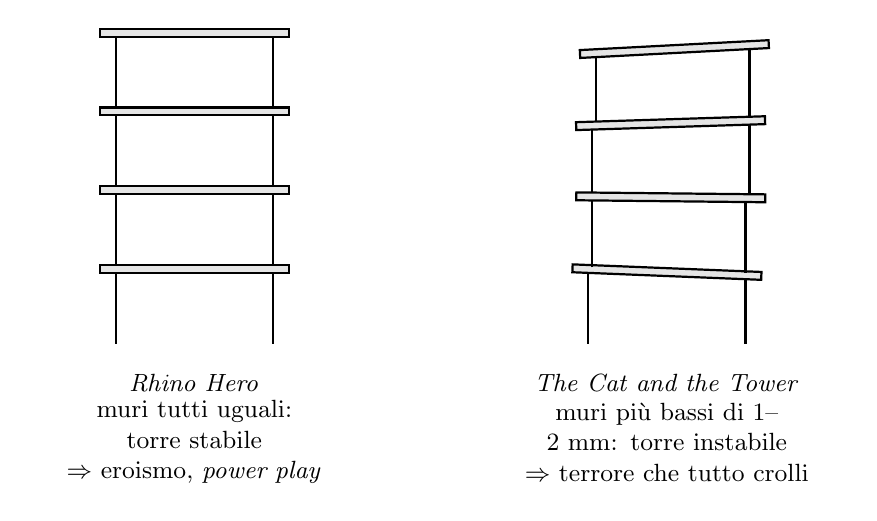
\begin{tikzpicture}[font=\small, x=1cm, y=1cm]
  % Rhino Hero: piani regolari
  \begin{scope}[shift={(0,0)}]
    \foreach \y in {0,1,2,3}{
      \draw[thick] (0,\y) -- (0,\y+0.9);
      \draw[thick] (2,\y) -- (2,\y+0.9);
      \draw[thick, fill=gray!20] (-0.2,\y+0.9) rectangle (2.2,\y+1.0);
    }
    \node[align=center] at (1,-0.5) {\emph{Rhino Hero}};
    \node[align=center, text width=4cm] at (1,-1.25)
      {muri tutti uguali: torre stabile\\$\Rightarrow$ eroismo, \emph{power play}};
  \end{scope}
  % Cat and Tower: muri di altezze diverse
  \begin{scope}[shift={(6,0)}]
    \draw[thick] (0,0) -- (0,0.9);   \draw[thick] (2,0) -- (2,0.82);
    \draw[thick, fill=gray!20, rotate around={-2.3:(0,0.9)}] (-0.2,0.9) rectangle (2.2,1.0);
    \draw[thick] (0.05,0.97) -- (0.05,1.82); \draw[thick] (2.0,0.9) -- (2.0,1.8);
    \draw[thick, fill=gray!20, rotate around={-0.6:(0.05,1.82)}] (-0.15,1.82) rectangle (2.25,1.92);
    \draw[thick] (0.05,1.92) -- (0.05,2.72); \draw[thick] (2.05,1.9) -- (2.05,2.78);
    \draw[thick, fill=gray!20, rotate around={1.8:(0.05,2.72)}] (-0.15,2.72) rectangle (2.25,2.82);
    \draw[thick] (0.1,2.82) -- (0.1,3.64); \draw[thick] (2.05,2.88) -- (2.05,3.78);
    \draw[thick, fill=gray!20, rotate around={3.0:(0.1,3.64)}] (-0.1,3.64) rectangle (2.3,3.74);
    \node[align=center] at (1,-0.5) {\emph{The Cat and the Tower}};
    \node[align=center, text width=4.4cm] at (1,-1.25)
      {muri più bassi di 1--2 mm: torre instabile\\$\Rightarrow$ terrore che tutto
      crolli};
  \end{scope}
\end{tikzpicture}
\caption{Stessa meccanica, paragame diverso: due torri di cartone. In \emph{Rhino Hero}
i piani sono regolari e la dinamica è quella dell'eroe che sale; in \emph{The Cat and
the Tower} alcuni muri sono di uno o due millimetri più bassi, e la torre, sempre
storta, trasmette paura e fragilità. Schema illustrativo, con le pendenze esagerate.}
\label{a10:fig:torri}
\end{figure}

% ---------------------------------------------------------------------
\section{Chiusura: ci si vede il 12}
\label{a10:sec:chiusura}

Mancano tre minuti, ``tempo per un'ultima domanda'', magari ``quella nell'angolino, un
po' timida''. Non arriva (``adesso non ce la faccio''). Gianmarco si smuta, ``il segnale
internazionale'' di chi sta per salutare, ma non ha domande; Ruggero lo invita
scherzosamente a dire anche solo ``cose stupide, tipo: oggi ho ucciso una mosca in
bagno''.

``Allora, gente, io vi saluto, e la lezione di oggi si conclude così.'' L'appuntamento è
\textbf{il 12}, con i \emph{pitch}: ``non fate scherzi, so che li avete, so che li potete
fare''. Al \emph{pitch} non ci sarà solo Ruggero: ci saranno anche \textbf{Beatrice} e
\textbf{Daniele}. ``Buona serata, buona cena, buon weekend.''

% ---------------------------------------------------------------------
\section*{Punti chiave del capitolo}
\addcontentsline{toc}{section}{Punti chiave del capitolo}

\begin{itemize}
  \item La \textbf{UX} è un primo strato tra la persona che si avvicina al gioco e
        l'ecosistema di regole: può essere ``un incredibile aiuto o un gigantesco
        ostacolo''. Regole perfette che non arrivano a chi gioca finiscono ``nel
        cestino''.
  \item I \textbf{quattro pilastri}: \textbf{immediatezza} (si capisce subito, senza
        sforzo: spade e scudi, il barile di petrolio, l'alloro dei punti vittoria),
        \textbf{efficienza} (un'azione complessa nel minor spazio: ``pesca una carta''),
        \textbf{memorabilità} (il +4 di \emph{Uno}, il simbolo di ``tappare'' di
        \emph{Magic}), \textbf{soddisfazione} (\emph{Parks}, \emph{Canvas}, \emph{Tiny
        Epic Mechs}). Sono indipendenti: le icone di \emph{Race for the Galaxy} sono poco
        immediate ma molto efficienti.
  \item Immediato per chi gioca abitualmente non vuol dire immediato per tutti; anche il
        \textbf{colore} fa parte del significato di un'icona.
  \item Il \textbf{wireframe} delle carte cambia durante il prototipo: togliere ciò che
        vale zero, ridurre il testo con le icone, spostare ciò che conta meno. Nei primi
        stadi: \textbf{carte funzionali, non carte belle}.
  \item \textbf{Accessibilità}: font per la dislessia, \emph{curb cut effect} (ciò che è
        più accessibile per qualcuno lo è per tutti), daltonismo da verificare con
        \textbf{Chromatic Vision Simulator}; i mancini e le carte a ventaglio.
  \item Il \textbf{paragame} estende al gioco il \textbf{paratesto}: tutto ciò che non è
        regole e non è fiction, ma incide sull'esperienza. I bordi sono zone grigie
        (i librogame, \emph{Lift It}).
  \item Le aree: \textbf{materialità} (legno, plastica, metallo, app, spessore e
        \emph{core} delle carte, \emph{standee}; clessidra contro timer),
        \textbf{formato} (font, misura delle carte, \emph{200 Word RPG}),
        \textbf{regolamento} (pagine, più libretti, video, glossario,
        \emph{playthrough}, \emph{play aid}), \textbf{scatola} (dall'armadio alla
        Kallax), \textbf{grafica e illustrazioni} (due mestieri diversi),
        \textbf{interfaccia analogica}, \textbf{ambiente} (il tavolo IKEA, il treno,
        \emph{Jenga} in aereo), \textbf{audio}, \textbf{contesto}, \textbf{lingua},
        \textbf{spazio urbano e ibridi digitali}, \textbf{inserti e setup}.
  \item Il paragame \textbf{incide sulle regole}: il formato limita la complessità
        delle regole, la clessidra cambia la tensione, la colonna sonora può essere una
        meccanica. Ai \emph{pitch} e alle revisioni Ruggero chiederà
        \textbf{``tantissimi perché''}.
  \item I casi studio vanno da \emph{Cuba Libre} (due regolamenti, diagrammi di flusso
        per i bot, brochure per fazione) a \emph{193 Days} (solo un mazzo), da
        \emph{Shenzhen I/O} (il manuale stampato) a \emph{Meltdown} (tessere di
        ghiaccio). Il test: ``\textbf{poteva essere di cartone?}''
  \item Il paragame non agisce direttamente sulle dinamiche: agisce sulle meccaniche
        (e sulla fiction), come tutto il design. Serve a far sì che \textbf{le intenzioni
        di design arrivino} a chi gioca, anche quando chi l'ha progettato non è al
        tavolo.
  \item Gli \textbf{inserti} non sono un dettaglio: nessuno ama il \emph{setup}, e un
        buon inserto lo accorcia. Il \emph{setup} si può anche rendere parte del gioco,
        nei giochi leggeri.
  \item \textbf{Ricerca e sviluppo} anche sul paragame: \emph{Rhino Hero} e \emph{The
        Cat and the Tower} hanno la stessa meccanica, ma muri di altezza diversa
        trasformano l'eroismo in terrore. \emph{Copy, transform, combine}, e
        \textbf{cross-modalità}.
\end{itemize}

%
%  Tutte le etichette di questo capitolo hanno il prefisso "a10:"
%  (a10:cap:..., a10:sec:..., a10:fig:..., a10:tab:...). Il capitolo è
%  autonomo: non contiene \ref verso altri capitoli.
%  Le figure e le tabelle sono ricostruzioni schematiche di quanto il
%  docente spiega a voce e mostra con le slide, non copie delle slide.
%  Dove la trascrizione è troppo rovinata per ricostruire un dettaglio
%  (un nome di gioco, una misura), il capitolo lo dice invece di
%  inventarlo.
% =====================================================================

\chapter[UX design e paragame]{UX design e paragame: l'interfaccia del gioco e
tutto ciò che non è né regole né fiction}
\label{a10:cap:paragame}

Questa è la \textbf{decima lezione} del corso di \textbf{Analog Game Design}, e
l'ultima prima del \emph{pitch} del 12 ottobre. Il suo tema è annunciato da Ruggero
già nei primi minuti, con un entusiasmo che non nasconde: ``oggi, lezione sul
paragioco. Quindi, sono carichissimo''. La lezione ha due metà. La prima è dedicata
alla \textbf{UX} (\emph{user experience}) del gioco, ``una roba gigantesca'' che non
riguarda solo il gioco analogico ma tutti i campi del design, e di cui il corso dà
solo le basi: che cosa sta tra la persona che si siede al tavolo e l'ecosistema di
regole, e quali sono i \textbf{quattro pilastri} di una buona UX
(\textbf{immediatezza}, \textbf{efficienza}, \textbf{memorabilità},
\textbf{soddisfazione}), mostrati con decine di icone e componenti di giochi veri, più
o meno riusciti. Chiude la prima metà una parte sull'\textbf{accessibilità}. Ruggero
la presenta come la parte di ``cose che magari già sapete''.

La seconda metà, sul \textbf{paragame} (o \emph{paragioco}), è invece ``una delle mie
parti preferite'', e ``sempre una parte delle lezioni abbastanza che spacca i
cervelli''. Il paragame è l'estensione al gioco del concetto letterario di
\emph{paratesto}: tutto ciò che di un gioco \textbf{non è regole e non è fiction}, ma
incide sull'esperienza di chi gioca. Il materiale dei dadi, lo spessore delle carte,
il numero di pagine del regolamento, la forma della scatola, il font, il tavolo su cui
il gioco verrà apparecchiato, la musica, il contesto culturale, la lingua, la città.
Dopo una carrellata delle aree progettabili, Ruggero mostra una lunga serie di
\textbf{casi studio}, ``da giochi più regolari a cose più \emph{deranged}'': un
wargame con sei brochure, un gioco di ruolo fatto solo di un mazzo di carte, un
videogioco che chiede di stampare un manuale, una gru da mettersi in testa, delle
tessere di ghiaccio da tenere in freezer. Il messaggio di fondo è uno, e Ruggero lo
ripete in molte forme: niente di tutto questo è ``contorno''. Il paragame
\textbf{incide sulle regole} e sull'esperienza, e chi progetta ``può lavorarci
attorno'' solo se ci ragiona. Per questo, ai \emph{pitch} e alle revisioni, il
docente chiederà ``tantissimi perché''.

La lezione è \textbf{online} e la conduce da solo \textbf{Ruggero}, condividendo le
slide. Si colloca con ogni probabilità \textbf{venerdì 9 ottobre 2026}\footnote{La
data non è detta, ma è ricostruibile. Nella lezione su Tabletop Simulator Ruggero
aveva indicato venerdì 9 ottobre come la data della lezione sul paragame. In questa
lezione dice che il \emph{pitch} ``del 12'' è ``lunedì'', e in chiusura gli studenti
si salutano con ``buon weekend''.}, dalle 17 alle 20 circa. Ci sono due pause: la
prima, di dieci minuti, alla fine della parte sulla UX (``alle sei ci ritroviamo
qua''); la seconda dalle \textbf{18:57} alle \textbf{19:05} (``ve ne do 8 per il numero
tondo''), prima dei casi studio. All'inizio sono collegati, tra gli altri,
\textbf{Tancredi} e \textbf{Gianmarco}; nel corso della lezione intervengono anche
\textbf{Tiziana} e \textbf{Lorenzo}\footnote{La trascrizione non distingue tra i due
Lorenzo del corso (Lorenzo Vergata e ``l'altro Lorenzo''); in un passaggio Ruggero
chiama ``Tancredi, Lorenzo. Lorenzo'', il che fa pensare che siano presenti
entrambi. Il capitolo scrive semplicemente ``Lorenzo''.}. Tiziana lascia la lezione
verso la fine (``Ciao, Tiziana'').

Tre avvertenze di lettura, le stesse dei capitoli precedenti. La prima: la
trascrizione è automatica e storpia moltissimi nomi, a cominciare da quelli dei due
argomenti della lezione. La UX diventa ``Wix'', ``l'usso'' e ``Wix design''; il
paragame diventa ``paragain'', ``paraghino'', ``paraggio'', ``parachain'',
``paragate'', ``paradigma'', ``paracadema'' e perfino ``guerra game''. \emph{Race for
the Galaxy}, il gioco più citato della serata, è ``Restore the Galaxy'', ``Rescord
Galaxy'', ``RIS4D Galaxy'', ``Risordiality'', ``Redsward Galaxy'', ``Days for the
Galaxy'' e ``Risk for the Gala''. Dove la ricostruzione è sicura, o molto probabile, il
capitolo usa la forma corretta e lo segnala in nota la prima volta; dove non lo è,
riporta la forma della trascrizione e lo dice. La seconda: durante le due pause la
trascrizione registra per decine di righe frasi senza alcun rapporto con la lezione,
ripetute in loop (``grazie a tutti per l'attenzione che ci ha spiegato'', ``qual è la
risposta che ci può essere?''), e subito dopo la seconda pausa qualche frase spuria
(``la situazione di oggi è la migliore dal 2000'', ``otto orecchie''). Sono artefatti
del riconoscimento vocale e il capitolo le ignora. La terza: gli studenti intervengono
spesso senza che la trascrizione segnali chi parla; il capitolo li nomina quando il
contesto lo rende chiaro e resta generico altrimenti.

\paragraph{Come leggere questo capitolo.} La lezione è costruita quasi interamente
su \textbf{immagini}: icone, carte, scatole, componenti, foto di giochi apparecchiati.
Nessuna di queste immagini è nella trascrizione. Il capitolo ricostruisce ciò che
Ruggero ne dice e, dove serve, descrive l'immagine a parole; quando un dettaglio
dell'immagine non è ricostruibile, lo segnala. Le tabelle riassumono le liste (i
quattro pilastri, le aree del paragame, i casi studio); le figure ricostruiscono gli
schemi (il posto della UX tra la persona e il gioco, le tre aree sovrapposte di
regole, fiction e paragame, il ventaglio di carte in mano). Le slide della lezione,
dice Ruggero, sono già nella cartella condivisa del corso. Qua e là, dei paragrafi di
\textbf{approfondimento} collegano la lezione ai libri di game design di riferimento
(soprattutto \emph{The Art of Game Design} di Jesse Schell) e alla letteratura sul
design dell'interazione e sul paratesto; sono segnalati come tali e non fanno parte
della lezione.

Il percorso del capitolo segue quello della lezione:
\begin{enumerate}
  \item l'attesa e due domande su Tabletop Simulator (sezioni \ref{a10:sec:attesa}
        e~\ref{a10:sec:tts});
  \item la \textbf{UX del gioco}: il suo posto nella \emph{pipeline} e i
        \textbf{quattro pilastri}, ciascuno con i suoi esempi (sezioni
        da~\ref{a10:sec:ux} a~\ref{a10:sec:soddisfazione});
  \item quante informazioni contiene una carta, il \textbf{wireframe} che cambia
        nel prototipo, l'\textbf{accessibilità} (sezioni da~\ref{a10:sec:informazioni}
        a~\ref{a10:sec:accessibilita});
  \item dopo la prima pausa, l'esercizio del \textbf{libro consigliato} e la
        definizione di \textbf{paragame} (sezioni \ref{a10:sec:libro}
        e~\ref{a10:sec:definizione});
  \item le \textbf{aree progettabili} del paragame, una per una (sezioni
        da~\ref{a10:sec:aree} a~\ref{a10:sec:pervasivo});
  \item dopo la seconda pausa, i \textbf{casi studio} (sezione~\ref{a10:sec:casi});
  \item la \textbf{discussione aperta} e la chiusura (sezioni
        da~\ref{a10:sec:discussione} a~\ref{a10:sec:chiusura}).
\end{enumerate}

% ---------------------------------------------------------------------
\section{L'attesa: il 12 ``sta nella pietra''}
\label{a10:sec:attesa}

Ruggero si collega con qualche minuto di ritardo (``pensavo di essere in ritardo'':
c'è stato un cambio di aula, ``ma siamo in orario''), e il clima è quello di fine
settimana. Si parla del caldo (``fa ancora troppo caldo per i miei gusti''), poi
Ruggero chiede come siano andate le lezioni con Beatrice (``interessante'',
``bene'') e come procedano i progetti di gruppo. Arrivano alla spicciolata gli
studenti del \textbf{gruppo 2}, che hanno appena fatto ``un piccolo meeting'' e
raccontano di aver \textbf{cambiato completamente} l'idea proposta. Ruggero non si
scompone: ``è normale''. C'è tempo fino al 12, ``però il 12 sta nella pietra''. Uno
studente, appena entrato, ammette di essere ``un po' incasinato col gioco'', e la
risposta è la stessa: ``ma è normale''. Quando qualcuno, scherzando, teme che al
\emph{pitch} i docenti ``sfasceranno'' le idee dei gruppi, Ruggero rassicura: ``no, non
vi sfasciamo niente''.

Ruggero aggiunge una promessa che riguarda direttamente il \emph{pitch}: la lezione
di oggi è ``proprio fatta apposta'' per chi ha ancora ``qualche buco di dubbio''. In
particolare la seconda parte darà ``delle idee intense'', che ``potrebbero portarvi a
riparlare tra di voi di varie cose in gruppo''; ed è sicuro che ``questo porterà lunedì
ad avere dei \emph{pitch} incredibili''.

Come al solito, prima di cominciare apre lo spazio per ``domande, dubbi, consigli,
insulti'', ``altrimenti stiamo qui in silenzio a osservare lo scorrere del tempo, e lo
sapete che non fa piacere a nessuno''. E annuncia il tema: ``UX design e paragame''.
Sulla prima parte, ``molte persone tra voi già sono sul pezzo'', perché la UX ``non è
una cosa esclusiva del gioco da tavolo'' ma tocca tutti i campi del design; la seconda,
invece, nelle edizioni passate è ``sempre una parte delle lezioni abbastanza che spacca
i cervelli. Quindi, non vedo l'ora''.

% ---------------------------------------------------------------------
\section{Due domande su Tabletop Simulator}
\label{a10:sec:tts}

Una studentessa ne approfitta per due domande ``molto semplici'' su Tabletop
Simulator, il software della lezione precedente\footnote{La trascrizione non dice chi
fa le domande; dal contesto è una persona che sta lavorando a un gioco ``per conto
mio'', fuori dal progetto di gruppo.}.

\paragraph{Prendere un mazzo intero senza tenere premuto.} La prima domanda riguarda
un fastidio pratico: per prendere un mazzo di carte intero, e non una carta sola,
bisogna tenere premuto il tasto del mouse per un paio di secondi. C'è una scorciatoia?
Ruggero ricorda prima quella per \textbf{pescare}: basta passare col mouse sopra il
mazzo e, senza cliccare, premere sulla tastiera il \textbf{numero} di carte da pescare
(``premo 5 e mi dà 5 carte in mano''). Ma la studentessa vuole \emph{spostare} il mazzo
intero, e le capita spesso. ``Che io sappia, bisogna tenere premuto'', risponde
Ruggero, che non ne ha mai avuto bisogno: se capita spesso, forse è ``più un problema
di logistica di come il modulo è \emph{set up}'', e si risolve ``setappando il modulo
bene''. Forse esiste un ``control-click'', ``non credo ci sia, ma chi può dirlo. Se lo
scopri, dimmelo''.

\paragraph{Simulare le luci.} La seconda domanda riguarda il gioco a cui la
studentessa lavora: un gioco con un \textbf{lumino} che proietta un'ombra, giocato
``tutto al buio''. Su Tabletop Simulator ha visto un modulo che simula le luci: si può
fare? ``Serve script? Assolutamente, per forza.'' E Ruggero sconsiglia ``fortemente''
di testare su TTS cose che lo richiedono: lì ``si apre il vaso di Pandora degli
script'', una cosa impegnativa che il corso non copre perché usa \textbf{Lua} come
linguaggio di programmazione, e fare ``delle lezioni di Lua apposta per dei casi
limite'' non ha senso nel programma. La studentessa chiede se basti copiare l'asset di
quel modulo. ``Puoi copiare l'asset se lo salvi'', ma dipende da come è stato
costruito. Se chi l'ha creato è stato ``furbo'', lo script è dentro l'asset stesso; ma
a Ruggero è capitato di trovare moduli con \textbf{script diffusi}, in parte in un
componente e in parte in un altro: se se ne copia uno solo, ``si rompe tutto e non
funziona''. Ruggero non conosce quel modulo: ``poi fare un po' di prove, sicuramente''.

\paragraph{Approfondimento: perché il gioco ``al buio'' è un tema di questa lezione.}
La domanda è più vicina all'argomento della serata di quanto sembri. Un lumino che
proietta ombre su un tavolo buio è un elemento di \emph{paragame} (luce, materiali,
ambiente) che diventa una meccanica: proprio il tipo di intreccio che Ruggero mostrerà
con \emph{Nyctophobia}, \emph{Scandal in the Deep} e \emph{Meltdown}
(sezione~\ref{a10:sec:casi}). Ed è anche un buon esempio del limite pratico del
prototipo digitale: ciò che dipende dalla fisica e dalla percezione (la luce, il peso,
la temperatura) si simula male in un software, e va provato sul tavolo vero.

% ---------------------------------------------------------------------
\section{La UX nel gioco: uno strato tra la persona e le regole}
\label{a10:sec:ux}

Ruggero condivide lo schermo e apre le slide: ``UX design e paragame'', una lezione
``divisa più o meno in due'', con ``una pausa a metà'' (``non sarà tutta una
mitragliata secca di cose''). La seconda parte sarà ``contemporaneamente un po' più
intensa, ma anche un po' più \emph{relaxed} della prima. Lo so, mi direte: com'è
possibile? Lo vedrete''.

Si parte dalla UX, con una premessa: è ``una roba gigantesca'' e ``questo non è un
corso di UX design''; la lezione si limita a dare ``delle basi su cui ragionare''. Gli
esempi saranno quasi tutti di \textbf{giochi da tavolo}, e non per caso: è un genere
che, più di altri, ``ha richiesto in passato un uso della UX fatto meglio'' rispetto,
per esempio, a un gioco di ruolo, o a un LARP in cui ``non è detto che venga neanche
usato il materiale stampato''.

\subsection{Dove sta la UX}

Il punto di partenza è una \emph{pipeline} che la classe ``dovrebbe già sapere'': una
\textbf{persona} che vuole giocare, il \textbf{gioco} (l'ecosistema di regole) e
l'\textbf{esperienza} che ne nasce. Il lavoro della UX ``sta qua in mezzo'': è ``un
primo \emph{layer} tra la persona che si approccia al gioco e l'ecosistema di regole
del gioco'' (figura~\ref{a10:fig:pipeline}). E ``spesso non ci si pensa, ma può essere
un incredibile aiuto o un gigantesco ostacolo''. Si può avere un ecosistema di regole
``lisciissimo, pulitissimo, fantastico'', in cui ``funziona tutto, bilanciato tutto'';
``ma se a livello di interfaccia questa roba non arriva, non si riesce a giocare, non si
riesce neanche a capire come giocare. Quel gioco finisce nel cestino''.

Di qui la regola: quando si progetta un gioco ``non ragioniamo solo alle meccaniche
del gioco, ma anche a cosa c'è davanti al gioco''. Che cosa c'è ``prima ancora delle
questioni di meccaniche, delle regole, ma anche prima del manuale'': il regolamento in
quanto oggetto, ``come sono fatte le carte, come il gioco è apparecchiato sul
tavolo''.

\begin{figure}[htbp]
\centering
\begin{tikzpicture}[
  font=\small,
  box/.style={draw, thick, rounded corners=3pt, minimum height=1.1cm,
              text width=2.5cm, align=center},
  ux/.style={draw, thick, dashed, rounded corners=3pt, fill=gray!15,
             minimum height=1.6cm, text width=2.6cm, align=center},
  arr/.style={-{Stealth[length=3mm]}, thick}
]
  \node[box] (p) {\textbf{Persona}\\che vuole giocare};
  \node[ux, right=0.9cm of p] (u) {\textbf{UX}\\icone, carte, regolamento,
    tavolo apparecchiato};
  \node[box, right=0.9cm of u] (g) {\textbf{Gioco}\\ecosistema di regole};
  \node[box, right=0.9cm of g] (e) {\textbf{Esperienza}};
  \draw[arr] (p) -- (u);
  \draw[arr] (u) -- (g);
  \draw[arr] (g) -- (e);
  \node[below=0.35cm of u, text width=3.4cm, align=center, font=\footnotesize]
    {``un incredibile aiuto\\o un gigantesco ostacolo''};
\end{tikzpicture}
\caption{Il posto della UX nella \emph{pipeline} persona--gioco--esperienza: un primo
strato tra chi si avvicina al gioco e l'ecosistema di regole. Se questo strato non
funziona, anche regole perfette non arrivano a chi gioca.}
\label{a10:fig:pipeline}
\end{figure}

\subsection{I quattro pilastri}
\label{a10:sec:pilastri}

Per progettare la UX di un gioco, Ruggero dà ``quattro pilastri che è bene tenere a
mente'': una buona UX ha \textbf{immediatezza}, \textbf{efficienza},
\textbf{memorabilità} e \textbf{soddisfazione} (tabella~\ref{a10:tab:pilastri}). Le
sezioni che seguono li vedono uno alla volta, ``nel dettaglio'', con esempi presi da
giochi reali. Una precisazione vale per tutti gli esempi: ``non vi serve sapere questi
giochi da dove arrivano''. Anzi, per alcune domande è meglio non conoscerli.

\begin{table}[htbp]
\centering
\small
\begin{tabular}{@{}p{2.6cm}p{5.4cm}p{5.2cm}@{}}
\toprule
\textbf{Pilastro} & \textbf{Che cosa vuol dire} & \textbf{Esempi della lezione} \\
\midrule
Immediatezza & si capisce subito il significato, con il minimo sforzo e senza
confusione & spade e scudi sui dadi; il barile di petrolio; la corona d'alloro dei
punti vittoria. Contro-esempi: \emph{Race for the Galaxy}, \emph{Argent} \\
Efficienza & racchiudere un'azione complessa nel minor spazio possibile & l'icona
``pesca una carta''; l'icona del punto vittoria; le icone di \emph{Race for the
Galaxy} (poco immediate, ma molto efficienti) \\
Memorabilità & restare in mente, così che a distanza di anni si ricordi ancora che
cosa fa & il +4 di \emph{Uno}; il simbolo di ``tappare'' di \emph{Magic}; le icone di
\emph{The Gallerist} \\
Soddisfazione & ``bonus point'': interagire con la grafica e i componenti è piacevole,
gratificante & il tracciato a frecce di \emph{Parks}; le carte trasparenti di
\emph{Canvas}; le armi in miniatura di \emph{Tiny Epic Mechs} \\
\bottomrule
\end{tabular}
\caption{I quattro pilastri di una buona UX secondo Ruggero, con gli esempi mostrati
a lezione.}
\label{a10:tab:pilastri}
\end{table}

% ---------------------------------------------------------------------
\section{Immediatezza}
\label{a10:sec:immediatezza}

Un elemento grafico è \textbf{immediato} quando ``comprendiamo subito il significato
di quello che vuole fare, con il minimo sforzo e senza confusione''. Il contrario è
chiaro: se vediamo una cosa e non capiamo che cosa fa, dobbiamo sforzarci, ci
confonde, ``magari facendoci anche sbagliare le regole'', e allora ``quella roba lì è
da buttare nel cestino''.

\subsection{Un tiro di dadi}

Il primo esempio è un \textbf{tiro di tre dadi} di un gioco che nessuno sa quale sia.
Le facce uscite mostrano \textbf{due spade}, \textbf{uno scudo} e \textbf{un fulmine}.
``Che cosa ci dice questo lancio di dadi?'' Le risposte arrivano subito: ``che siamo
stati fulminati'', poi, più seriamente, ``due attacchi, una difesa, e il fulmine non
saprei''. A livello di \emph{vibes}, è ``un lancio di combattimento, evidentemente'',
``perché ci sono le spade, gli scudi'' (``diciamo, combattimento sotto la pioggia col
fulmine'', scherza Ruggero). E in che tipo di gioco potrebbe stare? Uno studente pensa a
qualcosa come \emph{Civilization}, la conquista di un territorio; un altro a un gioco
fantasy, e cita un titolo che la trascrizione rende ``Cronache di Havel''\footnote{Con
ogni probabilità \emph{Le Cronache di Avel} (\emph{Chronicles of Avel}), gioco fantasy
cooperativo con combattimenti a dadi. Il gioco della slide, invece, non viene
nominato.}.

Il punto è che tutti hanno capito \textbf{immediatamente} che le spade sono attacco e
lo scudo è difesa, e che il tiro è ``più aggressivo che difensivo''; e nessuno sa che
cosa sia il fulmine. ``Ed è sempre così, quando io uso questo esempio.'' Spade e scudi
sono usati ``in talmente tanti giochi'', a livello di \textbf{euristiche personali}, che
si capiscono ``al volo anche se non sapete i dettagli di questo gioco'': non si sa come
funzionano il combattimento, la difesa, la vita, ma si sa che due spade e uno scudo
fanno un tiro aggressivo. Il fulmine, nel gioco, è \textbf{l'attivazione di
un'abilità}, ma è ``un'icona poco adatta a fare questo'', perché nessuno l'ha
riconosciuta come tale. Ed è normale: è molto più difficile trovare un'icona che
rappresenti ``in generale un'abilità, che può essere potenzialmente qualunque cosa'',
mentre spada e scudo sono di fatto delle \textbf{sineddoche}, ``delle metafore, in
questo caso, di \emph{ti sto attaccando} o \emph{mi sto difendendo}''.

\subsection{Quattro risorse}

Il secondo esempio sono le icone di \textbf{quattro risorse}, in alto a destra nella
slide. ``Chi è che sa da quale gioco vengono?'' Nessuno: ``best result'', perché la
domanda ``crolla'' se si conosce già il gioco. Le icone riproducono i segnalini di
legno delle risorse, con il loro colore e la loro forma. Che cosa rappresentano?

Le risposte della classe sono istruttive. Uno studente va ``più sul colore che sulla
forma'': il giallo è il grano, il grigio è la pietra, il marrone ``direi legno''.
\textbf{Tancredi} vede nella quarta, color ottanio, il \textbf{petrolio}, ``perché mi
sembra di qualche gioco che avevo provato''. Tiziana nota che ``la forma è
contraddittoria'', non corrisponde al colore; e una studentessa confessa di vederci
tutt'altro: ``una bara, una lapide, il lumino dove si mette il cero e una colonna che
sorregge'', insomma un cimitero.

Ruggero scioglie l'enigma partendo dalle due più semplici. Il \textbf{legno} ``nessuno
lo sbaglia'': è a forma di tronco tagliato, nei limiti di un piccolo componente. Quella
indicata come pietra è in realtà \textbf{metallo}, ma nel gioco non si confonde: il
gioco è ambientato in un mondo \emph{dieselpunk}\footnote{La trascrizione dice ``in cui
fai è site''. Le quattro risorse descritte (legno, metallo, grano e petrolio) e
l'ambientazione dieselpunk con giganteschi macchinari sono quelle di \emph{Scythe}
(Jamey Stegmaier, 2016), che è quasi certamente il gioco della slide.}, ``hai questi
giganteschi macchinari, per costruirli ti serve metallo'', e quindi quello viene preso
come metallo. Quello giallo confonde sempre chi non conosce il gioco, perché sembra
``un sacchetto di qualcosa di giallo'': le due risposte possibili sono oro o grano, e
qui è \textbf{grano}. E quello in cui ``non ci si sbaglia di solito'' è proprio la
risorsa color ottanio: ``Tancredi l'ha detto giusto, è petrolio'', perché usa ``la
colorazione dell'ottanio, che è il colore che culturalmente noi associamo alla benzina,
al gasolio, al carburante''. È forse l'icona più riconoscibile di tutte, perché è un
\textbf{barile di petrolio}. Il contesto, poi, conta: chi pensasse a un gioco come
\emph{Concordia}, ambientato nel Mediterraneo antico, ``non ha senso che sia petrolio''.

Ne esce un'osservazione in più: \textbf{non è solo la forma}; anche il \textbf{colore}
può essere fondamentale per riconoscere un'icona. ``Se io vi facevo il tronco viola,
non mi avreste detto legno. Se vi facevo il grano rosso, non mi avreste detto grano o
soldi, mi avreste detto qualcos'altro.''

\subsection{La corona d'alloro}

Terza domanda: l'icona in basso a destra, una corona con un \textbf{3}. ``Tre punti
vittoria.'' Perché? ``Perché c'è l'alloro.'' E perché l'alloro significa punti
vittoria? Perché l'alloro è un premio, un riconoscimento; e la \textbf{corona d'alloro}
``si è normalizzata, specialmente nei giochi da tavolo \emph{German}, negli Eurogame,
come simbolo dei punti vittoria''. In centinaia di giochi la coroncina d'alloro
rappresenta i punti, e chi trova un gioco con una corona d'alloro e un 3 sa che sono tre
punti.

Qui Ruggero fa una distinzione importante: \textbf{immediato non vuol dire immediato
per chi non ha mai giocato}, ``a tutte le persone''. L'alloro è immediato per chi gioca
abitualmente a giochi da tavolo, perché fa parte di un linguaggio condiviso. Poi,
``chiaramente, la forza di un'icona forte è essere immediata anche per chi non ha
giocato il gioco''.

\subsection{Le icone che fanno il contrario}

Ci sono però icone che fanno ``il contrario di quello che si dovrebbe fare di solito''.
Le prime due della slide, ``che ci crediate o no, sono due icone diverse
meccanicamente, che fanno due cose diverse''. Ruggero non dice che cosa fanno (``ho una
sanità mentale da risparmiarmi''): vengono da un gioco che la trascrizione chiama
``Gemoni''\footnote{Il titolo non è ricostruibile con sicurezza dalla trascrizione.},
``bel gioco'', ma con ``molte icone molto simili'', come queste due, che hanno i colori
praticamente invertiti e fanno cose diverse.

Poi due icone di \textbf{\emph{Race for the Galaxy}}\footnote{La trascrizione lo
storpia in quasi ogni occorrenza: ``Retribuzione'', ``Restore the Galaxy'', ``Rescord
Galaxy'', ``RIS4D Galaxy'', ``Risordiality'', ``Redsward Galaxy'', ``Days for the
Galaxy'', ``Risk for the Gala''. \emph{Race for the Galaxy} (Thomas Lehmann, 2007) è un
gioco di carte di fantascienza celebre per la sua iconografia densa.}. Gianmarco, che
lo conosce, viene escluso dalla domanda (``non lo chiederò a te, perché \emph{Race for
the Galaxy} è una maledizione''). Il gioco ha questa proprietà: ``per chi non lo
conosce, guarda le icone e pensa: questi sono pazzi, questo gioco non ha senso. Per
chi lo conosce, queste icone sono le più leggibili del mondo ed è immediato capire che
cosa fanno''. Ruggero prova a far indovinare la classe (``non do voti
all'interrogazione sulle icone di \emph{Race for the Galaxy}, anche perché sarebbe un
disastro per chiunque, \emph{me included}''), con un suggerimento: è un gioco
fantascientifico.

Sulla prima icona, Lorenzo prova ``annulla un comando'' (``ti sorprenderà sapere che
non è così''), un altro ``cambio colore'' (``ti piacerebbe; non è un gioco facile come
\emph{Uno}, questo''). Poi una studentessa tenta un'``archeologia ludica'': se ci sono
carte di vari colori, forse scartando una carta di quel colore succede qualcosa da
qualche altra parte. ``Un terzo l'hai beccata.'' Gianmarco completa: \textbf{scarti una
carta e la usi come risorsa} da mettere su un \textbf{pianeta}, ``che è quella cosa
tonda''.

``Adesso che abbiamo decifrato parte del linguaggio'', la seconda icona riesce meglio.
Uno studente: ``se hai tre carte blu, ottieni un esagono che non so cosa sia, e peschi
una carta?'' ``Vicinissimo, non sai quanto.'' L'icona parla di carte blu, ma non di
carte qualsiasi: di carte \textbf{usate come risorsa blu}, quelle appena viste. E non ne
servono tre: il numero dice che si può fare \textbf{fino a tre volte} la cosa che
segue, cioè ottenere un \textbf{esagono} (i punti, in questo gioco) e pescare una
carta. Tradotto: ``posso usare da una a tre risorse per prendere da uno a tre punti e
da una a tre carte''.

Infine l'icona in basso al centro, che Ruggero non spiega: ``è un'icona per cui
dovrebbero arrestare i graphic designer immediatamente''. Contiene, ``se non vado
errato'', una specie di \textbf{talismano} di carta scritta, uno \textbf{scudo} e
\textbf{due cappelli}, di cui uno in ombra. Viene da \textbf{\emph{Argent}}\footnote{
\emph{Argent: The Consortium} (Trey Chambers, 2015), gioco di piazzamento lavoratori
ambientato in un'università di magia.}: ``gioco bellissimo, icona illegale''. Che non
sia immediata, ``vi rendete conto anche voi''.

\paragraph{Approfondimento: convenzioni, affordance e linguaggi appresi.} Gli esempi
di Ruggero corrispondono a una distinzione classica del design dell'interazione. Alcuni
segni funzionano perché si appoggiano a \textbf{convenzioni} culturali molto diffuse
(la spada per l'attacco, il colore ottanio per il carburante, l'alloro per la vittoria);
altri richiedono di imparare un \textbf{linguaggio} specifico del singolo gioco, come le
icone di \emph{Race for the Galaxy}. Donald Norman, in \emph{The Design of Everyday
Things}, parla di \emph{significanti} (\emph{signifiers}) per indicare i segni che
comunicano che cosa si può fare con un oggetto, e osserva che le convenzioni sono
potenti proprio perché non vanno reimparate a ogni nuovo oggetto. Il limite che Ruggero
indica (immediato ``per chi gioca'' non è immediato ``per tutti'') è lo stesso: una
convenzione vale solo dentro la comunità che la condivide, e un gioco pensato per un
pubblico nuovo non può darla per scontata.

% ---------------------------------------------------------------------
\section{Efficienza}
\label{a10:sec:efficienza}

Il secondo pilastro è l'\textbf{efficienza}: ``comunicare più informazioni insieme,
alleggerendo l'aggregazione di informazioni''. Ruggero la spiega con ``due esempi
diretti''.

\paragraph{Pescare una carta.} La prima icona mostra un mazzo di carte. Che cosa fa?
``Peschi.'' Perché? ``Perché c'è un mazzo di carte.'' Ma Ruggero insiste: che cosa si fa
\emph{fisicamente}, ``a livello di propri atti fisici'', seduti al tavolo, per attivare
questa icona? ``Rivelo la prima carta del mazzo, prendo la prima carta del mazzo, e
poi\dots{} la metto in mano.'' Per chi gioca molto è una cosa semplicissima, ``solo
perché abbiamo giocato tonnellate di giochi''. Ma l'atto in sé è complesso: c'è un
componente che è un mazzo, che contiene tante carte; ne prendo la prima, la sollevo dal
mazzo e la aggiungo alla mia mano, di cui ora fa parte. ``È un'azione complessa, e
un'icona così ci riassume tutto questo processo.''

\paragraph{Il punto vittoria.} Lo stesso vale per l'icona del punto vittoria vista
prima. Che cosa si fa con un punto vittoria? ``Muoviamo la pedina.'' Se il gioco ha un
tracciato dei punti, quell'icona, ``nella sua piccolezza'', dice: prendi la tua pedina
dei punti vittoria e muovila avanti sul tracciato di tante caselle quanti sono i punti.

``Sono esempi piccoli e banali. Non sottovalutate questa cosa qua.'' Ruggero ne ricava
la definizione: un'icona efficiente \textbf{non} deve essere efficiente per chi non
conosce il gioco; un'icona efficiente ``è in grado di racchiudere al suo interno
un'azione complessa nel minor spazio possibile''. Ecco perché le due icone di \emph{Race
for the Galaxy} sono un caso interessante: sono \textbf{molto poco immediate}, ma
\textbf{molto efficienti}. In uno spazio piccolissimo danno tante informazioni e dicono
molto bene che cosa fare, ``una volta che abbiamo decifrato l'alfabeto di \emph{Race for
the Galaxy}''. I pilastri, insomma, sono indipendenti: un'icona può averne uno senza
l'altro.

% ---------------------------------------------------------------------
\section{Memorabilità}
\label{a10:sec:memorabilita}

Terzo pilastro: una buona icona deve ``rimanere nella mente, in modo da facilitare il
ricordo durante le partite successive''. Il criterio di Ruggero è concreto: ``se io gioco
un gioco e poi lo rigioco cinque anni dopo, e so ancora che cosa fa quell'icona, quello
è un buon gioco''.

\paragraph{Il +4 di \emph{Uno}.} La prima carta della slide: che cosa fa? ``Pescare
quattro carte.'' Chi pesca? Il giocatore successivo. Il gioco è \emph{Uno}. ``E quand'è
che hai giocato l'ultima volta?'' ``Boh. Almeno un paio d'anni fa.'' Non ci si ricorda
nemmeno quando, ma ci si ricorda che cosa fa la carta. Perché è una carta
\textbf{memorabile}: ``quando ti viene giocata contro, bestemmie''. Giocarla, o subirla,
dà ``un \emph{boost} emotivo tale'' che quello che fa diventa memorabile, ``quasi
memetico''.

\paragraph{Il simbolo di ``tappare''.} La seconda icona: dove nasce, che cosa chiede di
fare? Una prima ipotesi (``invertire il turno'') è sbagliata; poi uno studente fa
l'``ipotesi molto scontata'': \textbf{\emph{Magic: The Gathering}}. L'icona chiede di
\textbf{tappare} la carta, cioè di \textbf{ruotarla di 90 gradi}: una carta tappata ha
usato la sua abilità e non la si può riutilizzare nel turno. ``Quand'è l'ultima volta che
hai giocato a \emph{Magic}?'' ``Cent'anni fa.'' Eppure ci si ricorda ancora che quel
simbolo vuol dire ``prendi la carta e ruotala di 90 gradi''. Il motivo, qui, è diverso
da \emph{Uno}: è che il simbolo è \textbf{pervasivo}, ``è ovunque''; chi ha giocato a
\emph{Magic} l'ha incontrato per forza.

\paragraph{Le icone di \emph{The Gallerist}.} Le ultime due icone sono riconosciute da
uno studente, che ricorda il gioco ma non l'effetto: \textbf{\emph{The
Gallerist}}\footnote{\emph{The Gallerist} (Vital Lacerda, 2015), gioco in cui si
gestisce una galleria d'arte.}. La prima dà popolarità, la seconda soldi, in proporzione
ai \emph{meeple} presenti: un punto ogni due \emph{meeple} di un colore (magenta, nel
primo caso; marroni, nel secondo) oppure ogni \emph{meeple} bianco. ``Quindi, se ho
quattro magenta e un bianco prendo tre; se ho otto magenta prendo quattro.'' Chi ha
giocato a \emph{The Gallerist} se le ricorda, perché sono ``dappertutto in tutto il
gioco''. E sono icone che, quando te le spiegano la prima volta, ``vi sparate''; ``ma
dopo il primo turno nessuno va a riguardare nel regolamento che cosa fanno''.

Dai tre esempi escono tre strade diverse verso la memorabilità: l'\textbf{emozione}
(\emph{Uno}), la \textbf{pervasività} di un simbolo in tutto un sistema di gioco
(\emph{Magic}), la \textbf{ripetizione} dentro una singola partita (\emph{The
Gallerist}).

% ---------------------------------------------------------------------
\section{Soddisfazione}
\label{a10:sec:soddisfazione}

``Memorabili, immediate, efficienti: fantastico. Ma \emph{bonus point} se è anche
\textbf{soddisfacente}'': se interagire con l'aspetto grafico, con la UX del gioco, è
piacevole e gratificante. Tre esempi.

\paragraph{Il tracciato di \emph{Parks}.} In \emph{Parks}\footnote{\emph{Parks}
(Henry Audubon, 2019), gioco di escursioni nei parchi nazionali statunitensi.} il
tracciato su cui ci si sposta con i propri pedoncini è composto da \textbf{tessere}, e
ci si muove in una sola direzione, da sinistra verso destra. Le tessere hanno una forma
quasi a \textbf{freccia}, sono ``un po' inclinate in modo che si incastrino'', formando
una specie di nastro che indica la direzione. ``Potevano essere rettangoli? Sì, non
cambia niente meccanicamente.'' Ma incastrarle in ordine, oltre a essere memorabile
(perché ricorda la direzione), è anche ``molto soddisfacente''.

\paragraph{I quadri di \emph{Canvas}.} In \emph{Canvas}\footnote{\emph{Canvas} (Jeff
Chin e Andrew Nerger, 2021).} si compongono dei quadri con delle carte di
\textbf{plastica semitrasparente}: ogni quadro è fatto di \textbf{tre strati}
sovrapposti. Non solo gli elementi si combinano visivamente, ma anche il \textbf{nome
del quadro} viene generato dalle carte giocate: alcune carte danno la prima parte del
nome, altre la seconda.

\paragraph{Le armi di \emph{Tiny Epic Mechs}.} L'ultimo è un gioco di \emph{mech} che
combattono\footnote{La trascrizione dice ``Tiny Pic Max'': è \emph{Tiny Epic Mechs}
(Scott Almes, 2019).}, in cui i \emph{meeple} entrano dentro delle piccole
\textbf{armature di plastica}; e quando si cambia equipaggiamento, si mettono loro in
mano ``le piccole armi e gli scudini''. ``Meccanicamente, non cambia niente'':
l'equipaggiamento è comunicato anche dalle carte. Ma è molto soddisfacente, e ``ci
ricordiamo al volo che cosa abbiamo in mano, perché fisicamente il nostro \emph{meeple}
ce l'ha in mano'': un lanciagranate, uno scudo. E quando si cambia arma, si cambia non
solo la carta, ma anche il pezzettino.

\paragraph{Approfondimento: la soddisfazione come ``feedback'' fisico.} Schell, in
\emph{The Art of Game Design}, dedica all'interfaccia un intero capitolo e insiste su un
punto che questi esempi rendono evidente: un'interfaccia non serve solo a trasmettere
informazioni, ma a dare a chi gioca la sensazione di \textbf{controllo} e un
\textbf{feedback} piacevole a ogni azione. Nel videogioco si parla di \emph{juiciness},
la ``succosità'' delle reazioni alle azioni del giocatore; nel gioco analogico lo stesso
ruolo è svolto dal gesto fisico: l'incastro di una tessera, la sovrapposizione di un
foglio trasparente, l'arma infilata nella mano di una miniatura.

% ---------------------------------------------------------------------
\section{Quante informazioni porta una carta?}
\label{a10:sec:informazioni}

Dopo una breve verifica (``stiamo andando lisci''), Ruggero pone una ``domanda da
tenere conto sulla UX'': \textbf{quante informazioni stiamo usando?}

Sulla slide ci sono due carte di due giochi di carte di fantascienza con un tema molto
simile, la colonizzazione interplanetaria. Una è ancora di \emph{Race for the Galaxy}:
``pensavate che fosse brutta solo l'icona. E invece anche il \emph{wireframe} della
carta è molto brutto''. È un peccato, perché il gioco ``è bellissimo, incredibile'';
Ruggero, che sembra fare \emph{dissing}, lo possiede nell'edizione completa, ``molto
brutto da vedere, però glielo perdoniamo lo stesso, perché è molto bello da giocare''.
L'altra è di \emph{Age of Galaxy}\footnote{Esiste un
gioco con questo titolo (\emph{Age of Galaxy}), di tema e struttura compatibili
con la descrizione.}. Quale delle due contiene più informazioni?

Tiziana dice la seconda. Altri, tra cui Lorenzo e Gianmarco, la prima. Lorenzo, che
guarda anche le icone, pensa che abbiano le stesse informazioni; e un altro studente
osserva che la prima sembra averne di più solo perché è \emph{old school}: le schiaccia
e le sposta sui bordi. È una domanda ``molto divisiva'', dice Ruggero, e lo è sempre:
anche nelle lezioni passate, con classi più grandi, una parte risponde la prima e una
parte la seconda. ``Le grafiche parlano a persone diverse'', e persone diverse
percepiscono come più pesante l'una o l'altra. In termini di \textbf{funzionalità
meccaniche}, però, le aree importanti sono le stesse.

\subsection{L'icona capovolta}

La carta di \emph{Race for the Galaxy} ha poi delle scelte particolari. Di fianco al
nome c'è un'icona con un numero (il punto 3 dell'analisi della slide), ed è
\textbf{capovolta}. Perché? Le ipotesi della classe: è qualcosa che si disattiva; la
carta va tenuta coperta; ``devo girarmi la carta per sapere quanto do?'' La risposta è
un'altra: ``è al contrario perché non è per noi, quell'icona. Serve agli avversari,
serve ad altre persone dall'altra parte del tavolo. Loro devono sapere che cosa fa
quell'icona, e quindi è girata verso di loro''.

Ruggero ammette che si può ``voler male'' a \emph{Race for the Galaxy} ``in mille
modi'': per esempio perché riporta tutte le fasi del turno (1, 2, 3, \$, 4, 5) di fianco
alla carta, ``inclusi quelli che non abbiamo e che non ci interessano in questa
carta''; o perché nel riquadro di testo ripete esattamente la stessa informazione
dell'icona, ``ma via testo, rendendo quindi inutile l'iconografia''. ``Però in realtà,
per l'utilizzo fisico della carta, \emph{Race for the Galaxy} è molto intelligente.''
Le icone che sono per chi gioca la carta sono girate verso di lui, quelle per gli altri
verso gli altri. E il \textbf{retro} della carta si può usare come materiale, come ha
detto prima Gianmarco: le carte con il cerchio sono pianeti, e una carta a faccia in
giù sotto un pianeta è una \textbf{risorsa} (arancione, in questo caso, perché il pianeta
è arancione).

Uno studente obietta: se l'informazione del testo è ridondante, le informazioni della
carta sono cinque, non sei. No, risponde Ruggero: il \textbf{4} non indica solo che
cos'è il testo, ma anche la \textbf{fase} del turno in cui si attiva. È la stessa
informazione divisa in due parti, e sulla slide lui l'ha numerata separatamente
``per sanità mentale'', perché due frecce sullo stesso punto erano illeggibili. Allo
stesso modo, sulla carta di destra alcune voci sono accorpate (il punto 2), perché
stanno nello stesso blocco, quello delle icone risorsa.

\subsection{Una carta prima e dopo: il wireframe cambia}
\label{a10:sec:wireframe}

Il secondo esempio viene dal lavoro di Ruggero. È una carta di un gioco
\emph{Cyberpunk}\footnote{La trascrizione dice prima ``Severpunk'', poi ``Cyberpunk'',
e ``lo sapete già'', come se il gioco fosse già stato mostrato nel corso. Il titolo
esatto non è ricostruibile dalla trascrizione.} su cui ha lavorato, ``nelle parti
pre-andata in stampa'': a destra la versione finale, a sinistra le versioni precedenti.
``Ignorate il numero di pistole, che è stato ribilanciato'': in termini di informazione,
le carte sono rimaste praticamente uguali. Ma molte cose sono cambiate.
\begin{itemize}
  \item Uno \textbf{0} è sparito: ``tanto erano zero. Appesantiva senza motivo, e
        quindi è volato via. Non ci serve saperlo: basta che non mettiamo niente''.
  \item La dicitura \emph{starting} (carta iniziale) ha perso priorità, ``giustamente'',
        ed è stata spostata sotto il titolo. Non solo: le carte iniziali hanno il
        \textbf{nome in grigio}. Così, alla domanda ``come faccio a sapere se è una
        carta iniziale, in mezzo al mazzo?'', la risposta è: dal nome grigio invece che
        colorato.
  \item È stata introdotta un'\textbf{iconografia} per \textbf{ridurre il testo}: i
        testi delle prime versioni sono più lunghi di quelli delle ultime.
  \item Alcune cose hanno ricevuto un nome di \emph{flavor} (Ruggero cita le
        \emph{sticker condition}).
\end{itemize}
``La carta è la stessa.'' E questo è il tipo di ragionamento, e poi di test, che
Ruggero si aspetta nella \emph{pipeline} di prototipo dei gruppi: ``le vostre icone, i
vostri \emph{wireframe} cambieranno in corso d'opera, le cose verranno spostate. È
giusto che voi partiate con un'idea di come devono essere messe le cose''. Ma con una
raccomandazione netta: ``\textbf{io non voglio vedere carte belle, voglio vedere carte
funzionali} nei primi stadi''. Il gruppo di lavoro di Ruggero ha testato con le prime
carte ``per mesi'', e ``erano letteralmente bianche, con due linee, due scritte e due
iconcine''. Non era un test di \emph{look and feel}; di questo si riparlerà nella
lezione sul \emph{playtest}.

\paragraph{Approfondimento: ridurre il testo, non le informazioni.} I tre interventi
sulla carta \emph{Cyberpunk} (togliere ciò che vale zero, spostare in secondo piano ciò
che conta meno, sostituire testo ricorrente con icone) sono i tre strumenti classici
della \textbf{gerarchia visiva}. Nessuno di essi toglie informazioni utili: cambiano
l'ordine in cui l'occhio le incontra e lo sforzo necessario per leggerle. Un'icona che
sostituisce una frase ricorrente funziona però solo se è \emph{appresa}, e quindi va
spiegata una volta e ripetuta in modo coerente; è lo stesso compromesso tra
immediatezza ed efficienza visto con \emph{Race for the Galaxy}.

% ---------------------------------------------------------------------
\section{Accessibilità}
\label{a10:sec:accessibilita}

``Quando pensiamo alla UX, non dobbiamo pensare solo e unicamente alla parte di
funzionalità meccanica, ma anche all'\textbf{accessibilità}'': quanto il gioco è,
``come il nome fa intuire'', accessibile.

\paragraph{Font per la dislessia.} Il primo esempio della slide è un \textbf{font per
persone con dislessia}. Ce ne sono molti, ``anche gratuiti''; quello mostrato è
gratuito per progetti non commerciali. Sono font che rendono più facile la lettura dei
testi.

\paragraph{Il \emph{curb cut effect}.} Poi una domanda: qualcuno conosce il
\textbf{\emph{curb cut effect}}\footnote{La trascrizione dice ``curb effect''. Il nome
corrente è \emph{curb cut effect}, ``effetto del marciapiede ribassato''.}? Non è legato
ai font né alla grafica, è ``una cosa più a ombrello''. Il \emph{curb} è il
\textbf{marciapiede}: quei marciapiedi che, in corrispondenza delle strisce pedonali,
hanno ``la piccola salitina''. Perché ce l'hanno? Per permettere l'accesso alle persone
in sedia a rotelle. Ma questo ha cambiato il marciapiede anche per tutti gli altri: per
chi scarica i pacchi con il carrello, chi sale con la bicicletta, chi rientra in casa
con un trolley, le persone più anziane, per cui un gradino potrebbe essere un pericolo.
\textbf{Rendere una cosa più accessibile per qualcuno la rende più accessibile anche
per tutte le altre persone.}

\paragraph{Il daltonismo.} Il secondo strumento è un'app gratuita che Ruggero consiglia
``caldamente'' di avere sul cellulare (lui ce l'ha su tutti i telefoni di lavoro):
\textbf{Chromatic Vision Simulator}. Si fotografa il proprio prototipo, e l'app mostra
l'immagine con la visione regolare dei colori e con le tipologie più comuni di
\textbf{daltonismo}, facendo vedere se due colori diventano simili. Nell'esempio della
slide, con la tritanopia\footnote{La trascrizione dice ``tritanotapia''.} il giallo e il
rosa diventano molto simili, e in un'altra simulazione si confondono il verde e il
rosso. ``Scegliere i colori non è solo roba di \emph{vibes}, \emph{mood}'': può rendere
il gioco molto poco accessibile a chi è daltonico.

Ruggero porta la sua esperienza: nel suo gruppo di gioco abituale c'è un amico
daltonico, ``e ce ne accorgiamo subito se un gioco possiamo giocarlo insieme o non
possiamo giocarlo''. E chiude con un avvertimento: ``non ha senso impedire a una
persona daltonica di giocare un gioco da tavolo. Basta cambiare un colore, ragazzi,
davvero. Non cadete in queste cose qua. Io li guarderò, i vostri giochi, con
quest'app, quindi sappiatelo: usatela voi prima che la usi io su di voi''.

\paragraph{Approfondimento: qualche numero e qualche regola pratica.} Il daltonismo
congenito riguarda circa l'8\% degli uomini e lo 0,5\% delle donne di origine europea,
con forme più comuni nella confusione tra rosso e verde (deuteranopia e protanopia,
con le loro forme attenuate) e più rare nella confusione tra blu e giallo (tritanopia).
In un gruppo di quattro-cinque persone, la probabilità che ci sia almeno una persona
daltonica non è trascurabile. La regola pratica più diffusa nel design dei giochi è non
affidare mai un'informazione \textbf{solo} al colore: accompagnarlo con una forma, un
simbolo o un motivo (le carte con semi diversi, non solo colori diversi). È, di nuovo,
un \emph{curb cut}: un simbolo in più aiuta anche chi gioca con una luce scarsa o chi
guarda il tavolo dal lato opposto.

\medskip
Con questo la prima parte si chiude. ``Facciamo una pausetta'': dieci minuti, e
``alle sei ci ritroviamo qua'' per il ``blocco grosso'' della lezione, con un invito a
portare domande: ``non nascondetele''.

% ---------------------------------------------------------------------
\section{Dopo la pausa: il libro che avete consigliato}
\label{a10:sec:libro}

Al rientro nessuno ha domande, e Ruggero riassume il senso della prima parte: ``vi è
comunque utile ragionare sulle icone, su che cosa comunicano le icone in generale, sul
\emph{wireframe} delle carte'', anche per presentare le proprie carte. Poi passa alla
``parte succosa'': il paragame.

Comincia con un esercizio, in due tempi. Nel primo, ``non dovete rispondermi, dovete
pensarci un attimo'', trenta secondi. Bisogna pensare a un \textbf{libro}, con due
vincoli: deve essere un libro di \textbf{narrativa}, ``non un saggio'', e nel formato
più tradizionale (``non un fumetto, non una graphic novel, non un libro illustrato. Un
classico romanzo''); e deve essere un libro che è \textbf{piaciuto}, idealmente uno che
si è \textbf{consigliato a qualcuno}. ``Non ditemi qual è.''

Nel secondo tempo, invece, si risponde: \textbf{perché} l'avete consigliato? ``Non vi
sto interrogando, davvero: è utile per capire quello che verrà dopo.'' Le risposte:
\begin{itemize}
  \item Uno studente lo consiglia di solito dentro una conversazione: ``si sta parlando
        di qualcosa, e dico: ti consiglio questo, perché in questo punto c'è qualcosa di
        molto interessante'', che dà ``un valore aggiunto, una conoscenza in più''. Ma
        pensava a \emph{L'uomo che scambiò sua moglie per un cappello} di Oliver Sacks,
        che è un saggio, ``è il confine''; Ruggero chiede di restare sulla fiction.
  \item Un altro (Lorenzo, a quanto si capisce) consiglia un libro per il
        \textbf{genere}: ``il genere a me piace'', e quello è un libro fatto bene per
        quel genere. Fatto bene vuol dire: la \textbf{trama} è scritta bene, ``ha un
        buon nesso'', i \textbf{personaggi} sono buoni, e si vede che c'è della
        \textbf{cura} nella scrittura, ``la scelta delle parole, come sono formulate le
        frasi''. Poi le \textbf{tematiche}, ``emozioni particolarmente scritte bene,
        gestite bene''.
  \item Un'altra lo consiglia ``per ciò che mi ha suscitato'': le \textbf{emozioni}
        provate leggendolo, ``belle emozioni che può provare anche la persona a cui lo
        consiglio''. Ruggero rilancia: ``magari sai che a un tuo amico piacciono i libri
        che fanno piangere tantissimo, tu hai pianto tantissimo con un libro, e dici: sai
        che qua butti fuori un fiume''.
\end{itemize}

Poi la domanda vera: ``quel libro lo avreste apprezzato anche scritto in \textbf{Comic
Sans} a grandezza 60?'' Uno studente rivela il suo: \emph{Il club dei delitti del
giovedì}\footnote{La trascrizione dice ``Il Club dei Detti del Giovedì''. È il romanzo
giallo di Richard Osman (2020).}. In Comic Sans a corpo 60 ``vengono trenta miliardi di
pagine'', ma forse ``ci starebbe meglio di \emph{Dracula}, come \emph{vibes}''; magari
per un libro per bambini. E in \textbf{Times New Roman a corpo 6}? ``Non ci leggi, a
corpo 6''; ``però ne sono andati in stampa, così'', e almeno ``si sprecano pochi soldi,
perché sono pochissime pagine''. E se fosse stampato su \textbf{pagine nere, o con
fondo rosso gotico}? ``Per \emph{Dracula} magari va anche bene''; ``terribile, ci lasci
gli occhi''; ``il rosso sul nero fa malissimo''.

È a questo punto che una studentessa chiede chiarimenti su che cosa sia il paragame, e
un'altra persona fa notare a Ruggero che le slide non si vedono: ``non stai
condividendo''. ``Ragazzi, sono pazzo.'' Ruggero ricondivide e ripercorre in un attimo
le slide che aveva commentato a voce (il libro, il Comic Sans gigantesco, il font
piccolino, il nero su rosso), scusandosi anche con chi vedrà la registrazione: per
fortuna le sue slide ``non sono muri di testo, sono letteralmente a supporto di quello
che sto dicendo''.

Il senso dell'esercizio, intanto, è chiaro. ``Quando noi consigliamo un libro, è
difficile che lo consigliamo per come il libro è stampato.'' Anzi, si dice proprio
``non giudicare un libro dalla copertina''. Eppure la copertina, il font, la dimensione
del font, il numero di pagine, il \textbf{formato} (tascabile o no, un mattone, un A4
``ingestibile''), la copertina rigida o morbida \emph{cambiano l'esperienza di
lettura}. Ruggero aggiunge altri casi.
\begin{itemize}
  \item Se le pagine fossero \textbf{talmente sottili da risultare quasi trasparenti}?
        Qualche decennio fa è uscita un'edizione ``mammut'' di tutti i racconti di
        \textbf{Lovecraft} in un unico volume di circa 1100 pagine, che per stare in un
        solo libro aveva le pagine ``praticamente trasparenti'': ``impossibile leggerlo
        alla luce del sole''.
  \item Se le pagine fossero di \textbf{plastica}? ``Le posso leggere al mare, o nel
        bagno.'' Per un libro per bambini, ottimo; per \emph{Dracula}, forse no.
  \item E l'\textbf{ambiente} in cui si legge: in spiaggia, in treno, di notte sotto le
        coperte. ``Il \emph{mood} dell'ambiente in cui stiamo, mentre stiamo
        leggendo.''
\end{itemize}

% ---------------------------------------------------------------------
\section{Che cos'è il paragame}
\label{a10:sec:definizione}

``Il \textbf{paragame} è un'intera area di design che \textbf{non è fiction}, \textbf{non
è regole}, ma va a impattare l'esperienza'', e a volte si incrocia con quelle altre due
aree. Un font particolare, magari ``che va sul fantasy medievale'', può aiutare a
trasmettere la \textbf{fiction}, il \emph{world building}, il \emph{setting}. Ruggero lo
spiega con l'analogia da cui nasce il termine: ``questo è il \textbf{paratesto}. Il
paratesto nei libri, il paragioco nei giochi''.

Quando la studentessa chiede di nuovo se il paragame sia ``la modalità con cui il gioco
è realizzato fisicamente'', Ruggero precisa: è ``un termine che è l'estensione di
paratesto''. Con paratesto, in letteratura, si intendono ``tutte quelle parti di un
libro che non sono il suo contenuto, la sua fiction, ma sono tutte quelle parti di
forma, di formato'': il font, la dimensione e il colore del testo, ma anche il
\textbf{materiale}, lo spessore delle pagine, il formato del libro, la copertina rigida
o morbida (``magari di quella morbida, con quell'effetto \emph{matte} e vellutato che
amo tantissimo''). ``Sono tutti gli aspetti paratestuali, che sono di contorno.''
Il paragame è la stessa cosa per i giochi: ``gli aspetti di paragame sono tutti quelli
che ricoprono gli aspetti di un gioco che \textbf{non sono le regole e non sono la
fiction}''.

\subsection{I bordi sono zone grigie}

Il paragame ``può sforare, chiaramente, perché i bordi non sono dei muri, sono delle
zone grigie, non così definite'' (figura~\ref{a10:fig:aree}). L'esempio ``più diretto''
sono i \textbf{librogame}. Qualcuno ne ha giocati? Sì: il più famoso, forse, \emph{Lupo
Solitario}\footnote{La trascrizione dice ``un po' solitario''. \emph{Lupo Solitario}
(\emph{Lone Wolf}, Joe Dever) è la serie di librogame più nota in Italia.}. Come
paragame, i librogame sono libri: hanno una copertina, sono fatti ``come dei manuali,
tendenzialmente''. Ma il loro \textbf{formato} va anche in base alle \textbf{regole},
perché i paragrafi numerati sono le opzioni tra cui si sceglie. ``Non è un formato
separato dalle regole, è un formato che va a intrecciarsi''; e il font scelto, le
illustrazioni al loro interno, si intrecciano invece con la fiction.

\begin{figure}[htbp]
\centering
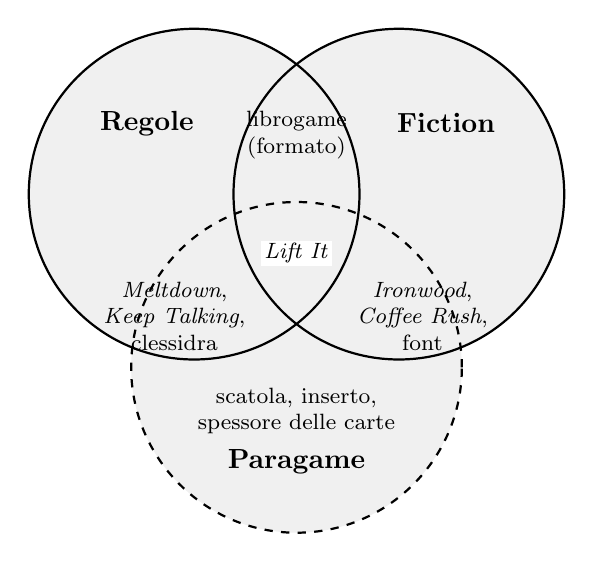
\begin{tikzpicture}[font=\small]
  \fill[gray!12] (0,0) circle (2.1cm);
  \fill[gray!12] (2.6,0) circle (2.1cm);
  \fill[gray!12] (1.3,-2.2) circle (2.1cm);
  \draw[thick] (0,0) circle (2.1cm);
  \draw[thick] (2.6,0) circle (2.1cm);
  \draw[thick, dashed] (1.3,-2.2) circle (2.1cm);
  \node[font=\bfseries] at (-0.6,0.9) {Regole};
  \node[font=\bfseries] at (3.2,0.9) {Fiction};
  \node[font=\bfseries] at (1.3,-3.4) {Paragame};
  \node[font=\footnotesize, align=center] at (1.3,0.75) {librogame\\(formato)};
  \node[font=\footnotesize, align=center] at (-0.25,-1.55)
    {\emph{Meltdown},\\\emph{Keep Talking},\\clessidra};
  \node[font=\footnotesize, align=center] at (2.9,-1.55)
    {\emph{Ironwood},\\\emph{Coffee Rush},\\font};
  \node[font=\footnotesize, align=center, fill=white, inner sep=1pt]
    at (1.3,-0.75) {\emph{Lift It}};
  \node[font=\footnotesize, align=center] at (1.3,-2.75)
    {scatola, inserto,\\spessore delle carte};
\end{tikzpicture}
\caption{Regole, fiction e paragame come tre aree con i bordi sfumati. Il paragame è
ciò che non è né regole né fiction, ma si sovrappone spesso a entrambe. La posizione
degli esempi riprende i commenti di Ruggero durante la lezione: \emph{Lift It} ``è al
centro'', \emph{Ironwood} aiuta soprattutto la fiction, \emph{Meltdown} e \emph{Keep
Talking and Nobody Explodes} soprattutto le meccaniche.}
\label{a10:fig:aree}
\end{figure}

\paragraph{Approfondimento: Genette e le ``soglie'' del testo.} Il termine
\emph{paratesto} viene dal critico francese Gérard Genette, che lo ha sistematizzato in
\emph{Soglie} (\emph{Seuils}, 1987). Per Genette il paratesto è ciò che fa di un testo
un libro e lo presenta al lettore: il titolo, il nome dell'autore, la copertina, le
dediche, le prefazioni, le note, ma anche il formato, la collana, la tipografia. È una
``soglia'' tra l'interno e l'esterno del testo, una zona di transizione che orienta la
lettura. L'idea di applicare lo stesso concetto ai giochi (paragame, paragioco) è
diffusa nei \emph{game studies}, dove il termine \emph{paratext} viene usato anche per
tutto ciò che circonda un gioco (\emph{trailer}, recensioni, guide, comunità). Nella
lezione di Ruggero il senso è più vicino a quello originale di Genette: le
caratteristiche materiali e formali dell'oggetto-gioco.

% ---------------------------------------------------------------------
\section{Le aree del paragame}
\label{a10:sec:aree}

``Su quali aspetti del paragame possiamo lavorare? E qui abbiamo l'ondata di robe.
Andiamo con calma: sono tante zone, ma sono sicuro che le vediamo tutte.'' La
tabella~\ref{a10:tab:aree} le riassume; le sezioni seguenti le vedono una per una.

\begin{table}[htbp]
\centering
\small
\begin{tabular}{@{}p{3.1cm}p{5.4cm}p{4.7cm}@{}}
\toprule
\textbf{Area} & \textbf{Domande da farsi} & \textbf{Esempi della lezione} \\
\midrule
Materialità & di che cosa sono fatti i componenti? Serve un'app? Quanto sono spesse
le carte? Clessidra o timer? & dadi di legno e di plastica; \emph{Lands of Galzyr} su
tablet e telefono; carte \emph{blue core}; \emph{standee} \\
Formato & come sono comunicati regole e testi? Che font, che dimensione, che misura
della carta? & \emph{Bureaucracy} di \emph{Magic}; il \emph{200 Word RPG} \\
Regolamento & quante pagine? Quanti libretti? Video, glossario, \emph{playthrough},
\emph{play aid}? & \emph{Irish Gauge}; \emph{Root}; riassunto delle icone \\
Scatola & dove andrà, nei negozi e a casa? & le vecchie scatole lunghe; la Kallax;
\emph{Dobro} \\
Grafica e illustrazioni & che cosa comunica l'aspetto visivo? Quante icone? &
\emph{Master of Rules}; \emph{Rolling Stock Stars}; \emph{A Feast for Odin} \\
Interfaccia analogica & com'è il \emph{wireframe}? Dove stanno le informazioni quando
il componente è in uso? & la carta di \emph{Magic}; la plancia di \emph{The
Gallerist}; le carte a ventaglio e i mancini \\
Ambiente & dove si gioca? Quanto spazio serve? Che suoni, che vibrazioni? & il tavolo
IKEA; il treno e l'aereo; \emph{Jenga} \\
Audio & serve una colonna sonora? & \emph{Escape: The Curse of the Temple} \\
Contesto & che cosa deve sapere chi gioca sul luogo e sulla cultura del gioco? &
\emph{Jakarta Traffic}; \emph{This War of Mine} \\
Lingua & il gioco dipende dalla lingua? & i giochi di Lacerda; \emph{Race for the
Galaxy}; \emph{Magic} \\
Spazio urbano e ibridi & la città, la stanza, il telefono come parte del gioco &
\emph{Pac-Manhattan}; \emph{Vroom}; \emph{World of Yoho} \\
\bottomrule
\end{tabular}
\caption{Le aree progettabili del paragame presentate a lezione, con le domande che
suggeriscono e gli esempi usati da Ruggero. Inserti e \emph{setup}, discussi alla fine
(sezione~\ref{a10:sec:inserti}), sono un'altra area della stessa famiglia.}
\label{a10:tab:aree}
\end{table}

% ---------------------------------------------------------------------
\section{Materialità}
\label{a10:sec:materialita}

La prima area è la \textbf{materialità}: ``le proprietà fisiche degli elementi di
gioco''. Legno, plastica, metallo. Prendiamo dei dadi classici di legno e dei dadi di
plastica: che cosa cambia? ``Il rimbalzo, il rumore, la sensazione al tatto.'' Sono
aspetti \textbf{cinestetici}, ``che assolutamente impattano''. Ma cambia anche altro,
``perché nel paragame spesso ci sono anche degli \textbf{aspetti culturali}''. In un
Eurogame, in un \emph{German}, si troveranno dadi di legno; in un \emph{American}, in un
\emph{dungeon crawler}, dadi di plastica. (Se n'era parlato, ``vagamente'', nella
lezione sui casi studio, a proposito dei componenti.)

\subsection{Il digitale come materiale}

Anche il \textbf{digitale} fa parte della materialità: se il gioco ha o richiede
un'app, un cellulare, un tablet, ``quello è un aspetto di materialità da considerare''.
Ruggero porta un esempio di un gioco che ha giocato, che la trascrizione chiama ``Lens
of Galsy''\footnote{Con ogni probabilità \emph{Lands of Galzyr} (Snowbright Studio,
2021), gioco d'avventura narrativo con app.}: ``molto carino, ma chiaramente pensato per
un tablet''. L'app ha tanto testo e tante cose a schermo, e sul cellulare, molto più
piccolo, ``non si vede niente''. ``L'app è la stessa, ma in base a dove lo stiamo
giocando, quel gioco può diventare un incubo di accessibilità, o qualcosa invece molto
più comodo da giocare.''

\subsection{Le carte non sono tutte uguali}

Quanto sono spesse le carte? Di che materiale sono? \emph{Blue core}, \emph{black
core}, \emph{white core}? ``Le carte non sono tutte uguali. Vi sembrano uguali perché le
usate da chi gioca, ma da produrre sono diverse.'' Quelle ``che si spaccano al volo'' si
riconoscono subito, perché sono le più economiche: di solito quelle di giochi come
\emph{Uno} o di giochi di carte ``più cheap da produrre'', in cui basta una pieghetta
per rovinare una carta ``forever and ever''. Altri giochi usano il \emph{blue core} o il
\emph{black core}; le carte di \emph{Magic}, per esempio, hanno il \emph{blue core}.

Ruggero semplifica la struttura: di solito una carta da gioco ha \textbf{tre strati},
lo strato con l'immagine sul fronte, quello con l'immagine sul retro, e in mezzo il
materiale che ne determina, tendenzialmente, la \textbf{rigidità}. ``Poi è più
complessa di così'', perché ci possono essere filigrane, texture e altro; ma la parte
centrale dice che cosa succede quando la carta si piega, o quando la si mescola male.

\paragraph{Le carte americane.} Una studentessa chiede delle carte da gioco americane,
``quelle di tela'', come le \emph{Bicycle}, che in Europa si vedono poco: c'è un motivo
per cui sono ``molto più fighe''? Sì: hanno una produzione che include \textbf{materiali
plastici} nella loro texture, che le rende più resistenti e crea un \textbf{attrito}
diverso. Sono carte che ``scivolano molto bene'' (``non ho più italiano, scusatemi''), e
infatti sono usatissime negli spettacoli di prestigiazione, perché si possono manovrare
velocemente, ``per chi le sa maneggiare; io no, di sicuro''. Le carte prodotte in Europa,
invece, hanno di solito un attrito molto più alto, e sono ``non fantastiche'' da usare
in modo ``sgaggio''.

\paragraph{Europa, America, Cina.} Lo stesso vale per i dadi: l'America fa un uso
abbondante di plastica nei giochi perché spesso produce in \textbf{Cina}, mentre
tipografie, stamperie e aziende che producono carte in Europa hanno ``molto poco
accesso'' a quei materiali. ``Quindi spesso siamo più forti nel legno e nella carta che
nella plastica.'' È ``un vaso di Pandora che a voi interessa il giusto'': per i progetti
del corso, quel tipo di finiture ``ve lo sognate, salvo pagare un bordello''. Ci sono
alcune fabbriche che possono fare cose bizzarre, nell'Est Europa e in Repubblica Ceca,
ma la maggior parte di chi produce stampa in Cina, oppure non usa quei materiali.

\paragraph{Miniature e \emph{standee}.} Stesso discorso per le miniature o gli
\textbf{\emph{standee}}, il cartoncino infilato in un piedistallo al posto della
miniatura di plastica. In un \emph{American} è facile trovare la plastica; in un gioco
prodotto e stampato in Europa, ``non trovate delle miniature di plastica'', perché non
c'è praticamente nessuna azienda europea di giochi da tavolo che possa stampare in
Europa la plastica a iniezione usata per le miniature; anche chi produce in Europa giochi
con parti di plastica le fa stampare in Cina. Per questo molti giochi europei degli anni
'90 e 2000, \emph{German} ed Eurogame, ``la plastica proprio la skippano'': se hanno
delle figure, sono \emph{standee}.

\paragraph{Approfondimento: che cosa fa davvero il ``core''.} Nella produzione di carte
da gioco lo strato centrale (\emph{core}) ha due funzioni: dà rigidità e soprattutto
rende la carta \textbf{opaca}, impedendo di vedere il fronte in controluce, cosa
essenziale in qualunque gioco con informazioni nascoste. \emph{Blue core} e
\emph{black core} sono nomi commerciali di cartoncini a più strati con un'anima
colorata scura. Sulle carte americane del tipo \emph{Bicycle}, il cartoncino è in
genere rivestito da una finitura goffrata e laccata (la cosiddetta \emph{air-cushion
finish}) che riduce l'attrito; le carte \emph{interamente} di plastica (PVC o acetato)
esistono, ma sono un prodotto diverso e più costoso.

\subsection{Clessidra o timer?}

``Occhio alla materialità, perché la materialità non va a impattare solo il paragame e
basta.'' Il classico esempio di materialità che impatta anche le \textbf{regole} è la
\textbf{clessidra}. Che differenza c'è tra un timer sul cellulare e una clessidra? Uno
studente risponde: ``la tangibilità''. Sì, e soprattutto quella che si chiama di solito
l'\textbf{informazione discreta}: con il timer si sa con precisione quando mancano un
secondo, due, tre, quattro secondi. Con la clessidra no: si vede chiaramente quando è
finita, ma ha ``quel pizzichino di incertezza che crea una tensione molto precisa che il
timer non ha''. Entrambi creano tensione, adrenalina, frenesia, ma in modo diverso; e
sapere quale dei due serve al proprio gioco ``non è così scontato''
(tabella~\ref{a10:tab:clessidra}).

\begin{table}[htbp]
\centering
\small
\begin{tabular}{@{}p{3cm}p{5cm}p{5cm}@{}}
\toprule
 & \textbf{Timer (cellulare)} & \textbf{Clessidra} \\
\midrule
Informazione & discreta e precisa: si sa quanti secondi mancano & continua e
incerta: si vede la sabbia scendere, ma non si sa con precisione quanto manca \\
Tensione & c'è, ed è ``contata'' & c'è, con ``un pizzichino di incertezza'' in più \\
Fiction & neutra, a meno di suoni scelti apposta & può essere diegetica (vedi il
fiammifero di \emph{Scandal in the Deep}, sezione~\ref{a10:sec:casi}) \\
Domanda da farsi & perché un timer e non una clessidra? & perché una clessidra e non
un timer? \\
\bottomrule
\end{tabular}
\caption{Timer e clessidra come scelta di materialità che incide sulle regole e sulla
tensione di gioco.}
\label{a10:tab:clessidra}
\end{table}

Qui Ruggero fa un annuncio che vale per il resto del corso: ``io ve lo ricordo, ve
l'avevo già accennato, ve lo ripeto: quando vedremo i \emph{pitch}, ma anche i vostri
progetti più avanti, nelle ultime lezioni, \textbf{io vi chiederò tantissimi
perché}''. Perché avete scelto una cosa, perché l'avete fatta, perché l'avete decisa.
``Se avete una clessidra e non un timer, io vi chiederò perché avete una clessidra e non
un timer. Perché avete la plastica, la carta, e così via. Voi dovete dirmi il perché
delle cose che fate.''

% ---------------------------------------------------------------------
\section{Formato}
\label{a10:sec:formato}

Il \textbf{formato} è il modo in cui sono comunicati, per esempio, regole e testi:
frasi o icone? Che font? Quanto è alto, che dimensione ha? E la carta, com'è fatta,
quanto è grande?

\paragraph{\emph{Bureaucracy}.} Il primo esempio è una carta di \emph{Magic} ``volutamente
fatta male'': \emph{Bureaucracy}, da una di quelle serie \emph{easter egg} (umoristiche)
che \emph{Magic} pubblica ogni tanto\footnote{La trascrizione aggiunge un dettaglio
sul simbolo dell'espansione che non è ricostruibile (``ha l'uomo rotto suonate come
simbolo''). \emph{Bureaucracy} appartiene alle espansioni parodiche di \emph{Magic}, le
cosiddette \emph{Un-set}.}. Per il testo è stato scelto un font piccolissimo (``mi
sembra che fosse un corpo 5, o addirittura 6''), per renderlo ``un muro di testo
oppressivo'': tematicamente coerente con il nome della carta.

\paragraph{La misura delle carte di \emph{Magic}.} Qualcuno sa quanto sono grandi le
carte di \emph{Magic}? ``Una dimensione da poker.'' In millimetri sono ``cifre
bizzarre'', perché in realtà la misura è di \textbf{3,5 per 2,5 pollici}\footnote{La
trascrizione riporta cifre storpiate (``88,4 per 69,5''). 3,5 per 2,5 pollici sono circa
88,9 per 63,5 millimetri; la misura nominale indicata di solito per le carte di
\emph{Magic} è 63 per 88 millimetri.}, ``in un sistema stupido americano di
misurazione'' (``ormai l'ho detto, è troppo tardi''). E in quella dimensione non c'è
tutto lo spazio che si vuole, perché una parte è dedicata all'\textbf{illustrazione}:
lo spazio per il testo, con il font e la dimensione scelti, è ancora più ridotto.
Questo non impatta solo il formato, ma anche le \textbf{regole}: ``una regola complessa
sarà difficile da scrivere in quello spazio'', e quindi il formato costringe a scegliere
regole che ci stiano dentro.

\paragraph{Il \emph{200 Word RPG}.} Un caso estremo: il \emph{200 Word RPG}, una sfida
in cui si scrivono giochi di ruolo completi in \textbf{200 parole}. Il paragame è il
formato stesso delle 200 parole: ``ditemi voi se non vi impatta le regole, quel
formato''.

``Non prendete questa cosa qua come del contorno, come una cosa che è un di più.
Questa roba qui vi va a impattare come voi create i giochi, e se lo sapete, potete
lavorarci attorno.''

% ---------------------------------------------------------------------
\section{Regolamento}
\label{a10:sec:regolamento}

Il \textbf{regolamento} è un'area a sé. Quante pagine ha? Una o quaranta? Che cosa
cambia? ``Se io vi dico: venite, c'è un party game, e tiro fuori un manuale da 60
pagine, che cosa succede?'' Succede che nessuno lo gioca.

\paragraph{\emph{Irish Gauge}: un caso positivo.} All'opposto, un caso ``incredibile'':
\emph{Irish Gauge}\footnote{La trascrizione dice ``Irish Gouge'' e attribuisce il gioco a
``Amable Holland'', più avanti ``Anne Blowland''. È \emph{Irish Gauge}, gioco
ferroviario di Amabel Holland.}, un gioco economico ferroviario ``bellissimo'', di circa
un'ora di partita, in cui si comprano azioni e si costruiscono ferrovie, con una
complessità significativa sul tavolo, ``un gioco comunque bello intenso''. E il
regolamento è \textbf{un singolo foglio di carta} ``che lascia zero dubbi dopo che lo si
è letto''. ``Bellissimo, irraggiungibile forse.'' È una sorpresa positiva; il caso
contrario (il party game da 60 pagine) è una sorpresa negativa che uccide il gioco.

\paragraph{QR code e video.} Chi gioca spesso avrà notato che sempre più regolamenti
hanno un \textbf{QR code} o un link a un video in cui le regole vengono spiegate.
Perché? ``Non sappiamo più leggere'' è ``la versione più nichilista''. La risposta ``più
banale e meno nichilista'' è che \textbf{le persone imparano in modi diversi}: un
regolamento scritto in un certo modo può andare benone per una persona ed essere un
disastro per un'altra.

\paragraph{Più libretti per lo stesso gioco.} Alcuni giochi hanno più di un libretto di
regole. \emph{Root}, per esempio, ha la \textbf{guida rapida} (il \emph{learn to play}),
scritta come un regolamento da leggere al tavolo, e la \textbf{Legge di Root}, scritta
come un \textbf{manuale tecnico}: paragrafi 1.1.1, 1.1.2, 1.1.3, 1.2.1 e così via, con
glossario. ``Il gioco è lo stesso. Lo si impara a giocare in entrambi i modi, ma parlano
a due persone completamente diverse.''

\paragraph{I costi.} Ogni scelta ha un costo. Un regolamento in più costa la
produzione di un regolamento in più, \textbf{a ogni copia} stampata. Il video è un costo
diverso: lo si paga una volta, all'inizio, lo si mette online ``e quel video lì è lì''.
``Se tu stampi 100 copie o ne stampi 10.000, il video non ti costa di più. Il
regolamento sì.''

\paragraph{Glossario, \emph{playthrough}, \emph{play aid}.} Altre domande: c'è un
\textbf{glossario}? Un \emph{playthrough}? Un \emph{play aid}? E le icone, dove sono
riassunte? Dove si trova di solito il riassunto delle icone? Due risposte, ``entrambe
vere''. Tancredi: \textbf{nell'ultima pagina del regolamento}, usata spesso proprio per
questo, perché si può tenere il regolamento girato sul tavolo e avere il riassunto
davanti. Tiziana: in un \textbf{\emph{play aid}}, un cartoncino, magari uno a persona,
con il riassunto delle icone. Quando l'uno e quando l'altro? Dipende da \textbf{quante
icone} ha il gioco. In \emph{Race for the Galaxy} un riassunto a testa non esiste,
``perché il riassunto delle icone di \emph{Race for the Galaxy} è così'' (e Ruggero
mostra quanto è lungo). In giochi con cinque, sei, una decina di icone è facile avere
una carta personale che le riassume, magari con il \textbf{flusso del turno} sul retro.

\paragraph{Il \emph{playthrough} e l'\emph{actual play}.} Più avanti, su richiesta di
uno studente (``Ruggero, non so se l'hai detto: il \emph{playthrough}?''), Ruggero torna
sul punto. Il \textbf{\emph{playthrough}} è \textbf{una giocata descritta}. Molti giochi
lo fanno spezzandolo in esempi: i classici esempi in cui ``Tizio e Caio fanno A, B, C,
poi Tizio fa B e Caio piange perché ha perso la partita''. Questi esempi non sono solo
un'applicazione delle regole: sono una descrizione di \textbf{che cosa fanno le persone
al tavolo}. Alcuni giochi, soprattutto di ruolo, includono il cosiddetto \textbf{\emph{actual
play}}: un'intera partita descritta, alternando le parti di \emph{roleplay} e quelle
meccaniche (``Tizio tira e fa 18, quindi apre questa cosa; poi Caio dice questa cosa con
il suo personaggio''). Dove si trovano\footnote{La trascrizione attribuisce la domanda a
qualcuno che si rivolge a ``Pietro''; con ogni probabilità è un errore di trascrizione
per ``Ruggero''.}? Sono ``comunissimi nei giochi di ruolo'': molti giochi di ruolo
contemporanei hanno esempi di \emph{actual play}, di solito in fondo al manuale. Gli
esempi sparsi nei regolamenti sono ``un'estrazione del \emph{playthrough}'', scritti con
la stessa idea; il \emph{playthrough} vero e proprio è l'esempio di partita completa. Nei
giochi da tavolo più commerciali è raro, ``perché le pagine dei regolamenti costano'', e
una partita completa prende molto spazio. Rientra quindi soprattutto nei giochi di
ruolo, che hanno già manuali da cento pagine e passa e non hanno il problema di stare
sotto le 16 pagine, ``perché sennò la gente si spaventa'' davanti a un regolamento da
20.

% ---------------------------------------------------------------------
\section{La scatola}
\label{a10:sec:scatola}

Nel formato rientra anche la \textbf{scatola}. Ruggero è convinto di averne già parlato
(``non abbiamo mai parlato delle scatole? Secondo me no'') e la affronta con una
domanda: come erano fatte le scatole del vecchio \emph{Risiko!} o del vecchio
\emph{Monopoly}? ``Basse e lunghe.'' Perché? ``Ci stava il tabellone''; ``si impilavano''.
La domanda, precisa Ruggero, non è che cosa c'era dentro, ma \textbf{dove doveva andare}
la scatola: nei negozi di giocattoli e, a casa, dove venivano messi i giochi trenta,
quarant'anni fa? Non nella libreria: \textbf{negli armadi}. ``Non era una questione
estetica'': l'armadio è stretto e lungo, e la scatola doveva entrare lì.

E oggi, dove vanno messi? In libreria. Quale libreria? La \textbf{Kallax}\footnote{La
trascrizione dice ``Callax'' e, a tratti, ``Galaxy''.} dell'IKEA, ``la libreria più
venduta del mondo''. Com'è fatta? ``\textbf{A cubi}.'' La scatola del vecchio
\emph{Monopoly} lì dentro non entra (``puoi metterla in cima, certo''). Ma se oggi un
editore vuole che il suo gioco entri ``nella libreria più venduta del mondo'', il gioco
deve entrare in un cubo. ``È tutto qui. \textbf{Una scelta dell'IKEA ha deciso che le
nostre scatole ora sono quadrate}.'' L'IKEA non ha convinto gli editori di niente: ``è
una roba che viene naturale, perché tutta l'umanità è intrecciata. Le decisioni che
prende qualcuno vanno a impattare qualcun altro''. Chi vuole che il proprio gioco sia in
vista in libreria deve fare i conti con il cubo.

Ruggero si concede qui una raccomandazione generale: ``se c'è una cosa che voglio che vi
portiate via da questo corso, una cosa'' (``poi, se fate anche giochi dopo, belli,
benissimo''), ``la cosa migliore per me, perché sono contento, ho fatto il mio lavoro,
posso morire in pace'', è questa: \textbf{ragionate quando fate le cose}. ``Potete
ragionare sulle cose quanto volete. Più ci ragionate, più avete aree operative su cui
fare le cose.''

\paragraph{Approfondimento: il ``formato Kallax''.} Il vano interno di una Kallax misura
circa 33 per 33 centimetri, per una profondità di poco inferiore ai 39. Non a caso un
gran numero di giochi da tavolo contemporanei di formato ``standard'' ha una scatola
quadrata di circa 30 centimetri di lato: è il formato che sta in un vano in piedi o
coricato, e che si impila bene. Molti editori lo indicano ormai esplicitamente tra i
vincoli di progettazione della scatola, insieme al peso e ai costi di spedizione.

% ---------------------------------------------------------------------
\section{Grafica e illustrazioni}
\label{a10:sec:grafica}

``\textbf{Graphic design e illustrazioni sono due cose diverse}. Non confondete le
cose.'' Le \textbf{illustrazioni} sono tendenzialmente l'\emph{art}: le immagini,
gli sfondi, i personaggi, i luoghi, la parte di \emph{world building}. Il
\textbf{graphic design} sono le icone, la UX. ``Non fate fare queste due cose alla
stessa persona, sennò di solito viene una porcheria.''

\subsection{Due edizioni, due destini}

Sulla slide ci sono due scatole: una con un omino che tiene sopra di sé delle forme, e
una con un'auto sotto un cielo stellato, una notte al neon. ``Sono lo stesso gioco'':
\emph{Master of Rules}\footnote{Il titolo è quello della trascrizione e non è stato
possibile verificarlo.}, ``un gioco bellissimo'', che nella sua edizione americana è
uscito con la prima scatola. ``Vi sorprenderà sapere che in America non è andato per
niente, nonostante sia un gioco incredibile. Qualcuno ha un'idea del perché?'' Le
risposte sono impietose: ``fa schifo'', ``sembra quelli che trovi in edicola''. E
dentro, dice Ruggero, ``è ancora più brutto''.

Uno studente lo provoca: ``io ho dei giochi che hanno copertine orrende da 100 euro'':
gli \textbf{Splotter}\footnote{Splotter Spellen, editore olandese noto per giochi
molto pesanti e per una grafica spartana.}. Ruggero non lo nega, ma ribalta la
domanda: la grafica degli Splotter ``è comprensibile perché la fanno così, ovvero perché
non gliene frega niente''; ma ``sarebbero giochi peggiori con una grafica migliore?'' ``La
risposta, nel tuo cuore, la sai: no.'' Le immagini danno un'esperienza, un \emph{look
and feel}.

Tiziana porta un caso concreto: un amico ha comprato \emph{Darwin's Journey}\footnote{
La trascrizione dice ``Darvis Journey''.}, ``un gioco che secondo me è bellissimo'', e
l'ha rivenduto, perché l'impatto grafico per lui è stato terribile: ``colori scuri sul
marrone''. ``Non riusciva a vederlo.''

Ruggero avrebbe potuto fare ``mille altri esempi'' di giochi usciti in due edizioni con
grafiche diverse, ``una che va a picco e non la vedete più, e l'altra che invece diventa
roba di culto''. Perché la grafica ha un impatto ``non solamente in termini di
leggibilità, ma anche di \emph{vibes}''. Lui, personalmente, non ci fa caso: ``io mi
gioco anche \emph{Rolling Stock Stars}'', che ``sembra fatto da marito e moglie su
Excel''. Ma altre persone vedono quella grafica e dicono ``non giochiamo a \emph{Rolling
Stock Stars}''. E finisce che ``il piccolo Ruggero'' lo gioca ``una volta ogni cinque
anni, perché nessuno vuole giocarci''. La conclusione: ``un gioco può beneficiare
dall'essere \textbf{non visivamente ostile} alle persone che lo vogliono giocare''.
Un altro studente aggiunge, a proposito di grafiche difficili, \emph{Terraforming
Mars} (``la carta con il cane''), e Ruggero si arrende: ``volete farmi stare male
oggi''.

\subsection{Il font, e quante icone}

Anche il \textbf{font} rientra nella grafica, non solo nel formato: il font del titolo,
il font dei contenuti. Ruggero cita un gioco che ha venduto ``proprio per il font che
aveva'', e promette di mostrarlo dopo, perché ``ci vuole del tempo per elaborare''
(lo farà nella discussione finale: è \emph{Al Rashid}, sezione~\ref{a10:sec:alrashid}).

Ultimo punto della grafica: \textbf{quante e quali icone} avete? Sulla slide c'è \emph{A
Feast for Odin}\footnote{La trascrizione dice ``Fist for Odin''. \emph{A Feast for
Odin} (Uwe Rosenberg, 2016).}: ``quel gioco lì ha 50 azioni diverse. Non devo dirvi
altro''. Ragionate sulle icone che avete.

\paragraph{L'intervento di Tiziana.} Tiziana porta un esempio di segno opposto: ha
giocato di recente a un gioco che la trascrizione chiama ``MNFR''\footnote{Il titolo
non è ricostruibile dalla trascrizione.}, abbastanza complesso, con varie tipologie di
azioni e una serie di cose che si succedono; ma le icone ``sono sempre quelle'', in
numero limitato, e una volta capite ``te le ritrovi in tutte le salse, nelle varie parti
e sezioni del gioco''. ``E questo aiuta molto.'' Ruggero concorda e cita di nuovo
\emph{The Gallerist} (``bellissimo, un capolavoro''): sono giochi in cui, se si fa un
buon lavoro sulle icone, il gioco ``non ti chiederà mai di andare a leggere il
regolamento durante la partita''. Lui ha giocato di recente un Eurogame di designer
giapponesi\footnote{La trascrizione dice ``Elder Tide degli stessi di Gisoji''; titolo
e autori non sono ricostruibili con sicurezza.}, con un \emph{setting} un po' fantasy, in
cui si costruiscono edifici su un'isola e ci si muove di porto in porto per vendere
risorse: ``ha tante icone, ma dopo i primi cinque minuti, per tutte le altre due ore
della partita, non abbiamo guardato il regolamento una singola volta, perché è tutto
chiaro, tutto immediato''. Si torna ai pilastri: immediatezza, efficienza,
memorabilità.

% ---------------------------------------------------------------------
\section{Interfaccia analogica}
\label{a10:sec:interfaccia}

La voce successiva è l'\textbf{interfaccia analogica}: ``si parla di
\emph{wireframing}, di solito''. È la struttura nuda della carta, quelle linee che, in
stampa, ``verranno abbellite da frame, cornici''. Ma il \emph{wireframe} è quello. ``Se
vi chiedo di disegnarmi a occhi chiusi su un foglio una carta di \emph{Magic}, voi sapete
come disegnarmela'': divisa a metà, al centro un rettangolino molto sottile, un
rettangolo più grosso in alto, uno più grosso in basso. ``Quella parte lì è una parte su
cui potete ragionare.''

\subsection{La scatola in piedi: \emph{Dobro}}

Anche la grafica della scatola è interfaccia. ``Se io prendo la scatola e la metto in
verticale, posso leggere il titolo?'' C'è una ``diatriba'' che Ruggero non apre
(``siete ancora persone sane di mente, non voglio rovinarvi la vita''): i giochi da
tavolo si mettono in libreria in verticale o in orizzontale? Lui fa un mix, ma molte
persone li mettono in verticale, e molte scatole non hanno il nome del gioco su tutti i
lati: alcune lo hanno solo per il lungo, e in verticale il nome è storto. L'esempio
positivo è \emph{Dobro}, di cui il suo gruppo ha rifatto la scatola per l'edizione
italiana: un lato lungo con il nome in orizzontale, il lato opposto con il nome in
verticale, e lo stesso sui due lati corti. ``Non importa come la mettete: un modo per
trovarla con il nome che si vede da fuori lo trovate sicuramente.'' Mentre ``ho delle
scatole in cui non si vede il nome, perché purtroppo non l'hanno messo su tutti i
lati''. Quindi: \textbf{la grafica della scatola non va lasciata al caso}, ``perché è
funzionale''. (``Mi sto arrabbiando, si vede, perché questa cosa mi fomenta.
Purtroppo per voi.'')

\subsection{Le opere sulla plancia di \emph{The Gallerist}}

Una studentessa chiede di chiarire: l'interfaccia analogica è il discorso della scatola
e della visibilità, o altro? Ruggero torna al \emph{wireframe}, ``cioè a come sono fatte
le carte'', e porta l'esempio di \emph{The Gallerist}: si acquistano opere d'arte da
esporre nella propria galleria, e la \textbf{plancia} personale raffigura la galleria.
Le tre tessere delle opere esposte si sovrappongono perfettamente ai \textbf{muri
disegnati sulla plancia}, ``andando letteralmente a mettere le opere in vista nella
nostra galleria''. Non è casuale: hanno pensato la grafica in modo che aiutasse a capire
che cos'è quel componente, e in modo che fosse anche soddisfacente. Di nuovo:
soddisfazione, efficienza, memorabilità, immediatezza.

\subsection{Dove stanno le informazioni quando le carte sono in mano}

Un altro aspetto dell'interfaccia è \textbf{dove si piazzano le informazioni}. Con le
carte da poker in mano, dove sono le icone? \textbf{In alto a sinistra}: quando le carte
sono aperte a ventaglio, ciascuna copre buona parte di quella precedente, e l'angolo in
alto a sinistra è ``la cosa più visibile'' (figura~\ref{a10:fig:ventaglio}).

Tancredi apre una parentesi sui \textbf{mancini}: ``io da mancino, tutte le volte che
apro le carte da poker, non vedo assolutamente niente''. Ruggero conferma (``ho degli
amici mancini, e se avete un gioco che non pensa ai mancini lo sapete al volo, perché
ve lo dicono''), e lo riconduce all'\textbf{accessibilità}: i mancini tengono in mano le
carte come tutti, ``è solo che per natura il ventaglio lo fanno nell'altro verso''. Molti
giochi per questo \textbf{duplicano} il seme della carta, mettendolo anche in alto a
destra. In alcuni giochi è più complicato: quando l'angolo in alto a sinistra ospita
icone meccaniche, come il costo, come in \emph{Race for the Galaxy} (``è il problema
minore di questa carta, mi sento di dire''), duplicare vuol dire affollare ancora di più
una carta già piena. ``Volete davvero duplicare le informazioni di questa carta
dall'altro lato? Io non lo farei.'' Non sempre si può; ma ``è assolutamente una
considerazione da fare''.

\begin{figure}[htbp]
\centering
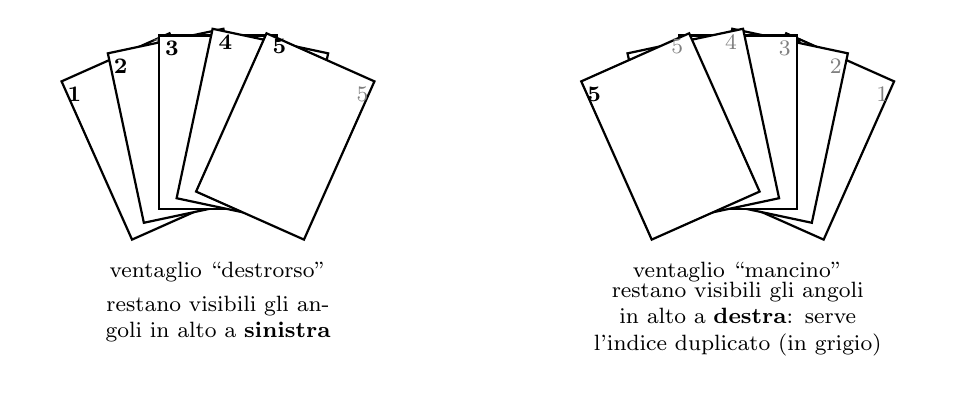
\begin{tikzpicture}[font=\footnotesize]
  % mano destrorsa: ventaglio verso destra
  \begin{scope}[shift={(0,0)}]
    \foreach \a/\i in {24/1, 12/2, 0/3, -12/4, -24/5}{
      \begin{scope}[rotate around={\a:(0,-2.6)}]
        \draw[thick, fill=white] (-0.75,-1.6) rectangle (0.75,0.6);
        \node[anchor=north west, inner sep=2pt] at (-0.75,0.6) {\textbf{\i}};
        \node[anchor=north east, inner sep=2pt, text=gray] at (0.75,0.6) {\i};
      \end{scope}
    }
    \node at (0,-2.4) {ventaglio ``destrorso''};
    \node[text width=4.6cm, align=center] at (0,-3.0)
      {restano visibili gli angoli in alto a \textbf{sinistra}};
  \end{scope}
  % mano mancina: ventaglio nell'altro verso
  \begin{scope}[shift={(6.6,0)}]
    \foreach \a/\i in {-24/1, -12/2, 0/3, 12/4, 24/5}{
      \begin{scope}[rotate around={\a:(0,-2.6)}]
        \draw[thick, fill=white] (-0.75,-1.6) rectangle (0.75,0.6);
        \node[anchor=north west, inner sep=2pt] at (-0.75,0.6) {\textbf{\i}};
        \node[anchor=north east, inner sep=2pt, text=gray] at (0.75,0.6) {\i};
      \end{scope}
    }
    \node at (0,-2.4) {ventaglio ``mancino''};
    \node[text width=4.6cm, align=center] at (0,-3.0)
      {restano visibili gli angoli in alto a \textbf{destra}: serve l'indice
      duplicato (in grigio)};
  \end{scope}
\end{tikzpicture}
\caption{Le carte a ventaglio. L'informazione più importante va nell'angolo che resta
scoperto; chi apre il ventaglio nell'altro verso, come molti mancini, vede l'angolo
opposto, e per questo molti giochi duplicano il seme o l'indice in alto a destra.
Schema illustrativo: l'ordine con cui le carte si sovrappongono dipende da come le si
apre.}
\label{a10:fig:ventaglio}
\end{figure}

Ruggero annuncia che su grafica e formato c'è ``un'altra cosa'', da riprendere dopo (lo
farà con gli inserti, sezione~\ref{a10:sec:inserti}).

% ---------------------------------------------------------------------
\section{Ambiente}
\label{a10:sec:ambiente}

\textbf{Dove} giocheranno le persone al vostro gioco? Su un tavolo, a letto, per terra,
in piedi? E \textbf{quanto spazio} prende il gioco? Qualcuno sa quanto spazio, al
massimo, deve prendere un gioco da tavolo \emph{family} per quattro persone? ``La sapete
nel vostro cuore, la risposta.'' Gianmarco: ``\textbf{il tavolo IKEA}''. ``Bravissimo,
Gianmarco, è sempre quello.'' Il tavolo IKEA più venduto: cercate quanti centimetri
misura. ``Se il vostro gioco non entra in quel tavolo, avete un grosso problema.''

E se è un \textbf{party game}? Allora deve stare nel \textbf{tavolino da caffè}
dell'IKEA, più piccolo, quello da divano, ``per un altro tipo di ambiente''. Se è un
gioco \emph{pocket}, portatile, deve stare nei tavolini da caffè, in quelli del
\textbf{treno}, in quelli dell'\textbf{aereo}. ``Quanto spazio prende il vostro gioco
apparecchiato non è casuale. Non lasciate al caso quella roba'', altrimenti succede,
come è capitato di vedere a Ruggero, di avere ``giochi in solitaria che prendono un
tavolo per sei persone''.

Il mezzo di trasporto ha poi un altro problema: il treno e l'aereo \textbf{si muovono}.
Il gioco può starci come spazio, ma i componenti? Uno studente ricorda le
\textbf{versioni magnetiche} di scacchi e dama, e una versione mini di \emph{Azul} con
le tessere che si incastrano. E Ruggero aggiunge: \emph{Jenga} ci sta, come spazio, nel
tavolino di un aereo. Perché nessuno ci gioca in aereo? ``Per le vibrazioni dovute al
movimento.'' Appunto: ``l'ambiente non è solo spazio. L'ambiente è anche suoni, è anche
vibrazioni, è un sacco di altre cose''.

\paragraph{Approfondimento: misurare il tavolo.} Le misure dei tavoli più diffusi
nelle case cambiano da modello a modello, ma un tavolo da cucina per quattro persone ha
spesso un piano tra gli 80 per 80 e i 120 per 75 centimetri, e un tavolino da caffè è
molto più piccolo (spesso intorno ai 90 per 55 centimetri). Il consiglio di Ruggero va
preso alla lettera: misurare il piano reale di riferimento e fare un \emph{mock-up} del
gioco apparecchiato a grandezza naturale, lasciando spazio per le mani, i bicchieri, le
plance personali e i mazzi degli scarti. È uno dei test più economici che si possano
fare con un prototipo.

% ---------------------------------------------------------------------
\section{Audio}
\label{a10:sec:audio}

Altra area progettabile: l'\textbf{audio}. Serve la musica nel vostro gioco? Alcuni
giochi usano una \textbf{colonna sonora} per dare il tempo. L'esempio è \emph{Escape:
The Curse of the Temple}\footnote{La trascrizione inciampa più volte sul titolo, e
Ruggero stesso si corregge (``scusatemi, perché in tedesco\dots''). Il gioco è
\emph{Escape: The Curse of the Temple} (Kristian Amundsen \O{}stby, Queen Games, 2012).}: un
gioco in tempo reale in cui bisogna uscire dal tempio entro la durata della colonna
sonora, ``sennò siete fritti''. E a intervalli la colonna sonora fa sentire dei
\textbf{colpi di gong} che attivano eventi meccanici nel gioco. Quindi la colonna
sonora non è ``solamente un timer, una grossa clessidra'': è un \textbf{elemento
meccanico} che, con l'audio, fa altre cose. E fa anche \textbf{fiction}: dà elementi di
\emph{world building}, certe \emph{vibes}. ``È chiaro che \emph{Escape} è molto Indiana
Jones: non avete una colonna sonora techno IDM a palla.''

% ---------------------------------------------------------------------
\section{Contesto}
\label{a10:sec:contesto}

``Al \textbf{contesto} non ci pensa quasi mai nessuno, ma è molto importante'', perché
informa il gioco, ``non solo in termini di \emph{world building}, ma anche in termini di
che cosa vuole che voi facciate''.

\paragraph{\emph{Jakarta Traffic}.} \emph{Jakarta Traffic}\footnote{Titolo come nella
trascrizione.} è un gioco sul traffico di Giacarta, ``che è molto ostile'': si naviga il
traffico per fare delle consegne, e molti elementi del gioco sono \textbf{culturali}.
Spiegare le meccaniche a chi non sa come è fatta Giacarta, culturalmente, rende il gioco
molto più complesso di quanto dovrebbe essere. Qui, secondo Ruggero, hanno fatto un
buon lavoro: il manuale aiuta a capire il contesto, e hanno perfino creato una colonna
sonora usando il traffico di Giacarta come \emph{sample}, per creare un certo
\emph{mood}.

\paragraph{\emph{This War of Mine}.} Ma il contesto non è solo \emph{setting}: può
anche \textbf{informare le scelte}. Qualcuno conosce il gioco da tavolo di \emph{This War
of Mine}\footnote{La trascrizione dice ``Diceworld Mine''.}? Qual è il suo contesto?
``È una guerra, ma non mi ricordo se è una guerra vera.'' ``È a metà'': non è scritto
apertamente, ma è palesemente l'\textbf{assedio di Sarajevo}. E soprattutto, non si
giocano militari: si giocano \textbf{civili}. Se ci si approccia al gioco ``con tutto il
bagaglio culturale dei giochi di guerra'', ci si aspettano cose che il gioco non può
dare, perché ``non è un gioco di soldati in guerra: è un gioco in cui c'è la guerra, ma
non è un gioco di guerra''. Queste cose si risolvono con un mix: in parte con testo,
\emph{flavor} e \emph{world building}, in parte con il paragame, con i materiali.

% ---------------------------------------------------------------------
\section{Lingua}
\label{a10:sec:lingua}

Anche la \textbf{lingua} è un componente. Alcuni giochi sono \textbf{indipendenti dalla
lingua}: in un gioco di Lacerda\footnote{Vital Lacerda, autore portoghese di Eurogame
pesanti, tra cui \emph{The Gallerist}.}, o nella maggior parte dei \emph{German}, sulle
carte non c'è testo, ``alla buon'icona''. Lo stesso \emph{Race for the Galaxy}, lasciando
stare il nome e l'effetto ricopiato sotto, si può giocare anche senza leggere l'inglese:
``mi basta sapere che cosa fanno quelle icone''. Così \emph{The Gallerist}, o \emph{Master
of Rules}. Altri giochi no: \emph{Magic} è molto difficile da giocare se le carte non sono
nella propria lingua.

% ---------------------------------------------------------------------
\section{La città, la stanza, il telefono}
\label{a10:sec:pervasivo}

``In quali altri modi posso impattare l'esperienza di chi gioca senza passare per le
regole e per la fiction?'' Sulla slide c'è un'immagine di
\textbf{\emph{Pac-Manhattan}}\footnote{La trascrizione dice ``Pac-Man Hatton''.
\emph{Pac-Manhattan} (2004) è un gioco urbano nato alla New York University, in cui
persone vere interpretavano Pac-Man e i fantasmi nelle strade di Manhattan.}: la città,
gli aspetti \textbf{pervasivi urbani} sono anch'essi paragame.

\paragraph{La stanza come pista.} Un altro esempio è un gioco di corsa cooperativo che
la trascrizione chiama ``Vroom''\footnote{Il titolo non è stato possibile verificarlo.}:
usa il \textbf{tavolo} come spazio di gioco e chiede di prendere degli \textbf{oggetti
della propria stanza} e metterli sul tavolo come ostacoli, ``fisicamente, proprio''.

\paragraph{\emph{World of Yoho}.} Infine \emph{World of Yoho}\footnote{La trascrizione
dice ``World of Yacht'', ``World of YOHO'', ``Word of Yoko''.}, un gioco di pirati che
chiede di usare il \textbf{cellulare} su un tabellone gigantesco. Il telefono è la
propria \textbf{nave}: quando lo si sposta, sullo schermo si muove la mappa, e le parti
di quella casella di mare diventano interagibili in digitale. ``Si poteva fare senza
cellulare? Sì, con un libro degli eventi gigantesco, una seccatura infinita. Mentre così
è una cosa immediata, che si spiega in tre minuti.'' Uno studente chiede se si giochi su
un tabellone normale: sì, il gioco arriva in scatola con il suo tabellone, che si mette
sul tavolo, e chiede semplicemente di usare il telefono come nave per tutta la partita.
Ogni persona usa il proprio telefono; e nelle battaglie navali ``vedi i proiettili che
vengono sparati da una nave, che vanno sul bordo del telefono ed entrano nell'altro.
Pazzi completi. Bellissimo''.

\medskip
Prima dei casi studio, una seconda pausa: ``sono le 57'', e Ruggero dà otto minuti
``per il numero tondo'': si riprende alle 19:05.

% ---------------------------------------------------------------------
\section{Casi studio}
\label{a10:sec:casi}

``Andiamo avanti nell'ultima parte'': i \textbf{casi studio}, per vedere ``come
applichiamo le cose che abbiamo appena visto a giochi particolari''. Ce ne sarebbero
``a tonnellate''; Ruggero ne ha scelti un gruppo ``che va da giochi più regolari a cose
più \emph{deranged}, come spesso succede'', e per ciascuno dovrebbe essere chiaro perché
è stato scelto. La tabella~\ref{a10:tab:casi} li riassume.

\begin{table}[htbp]
\centering
\small
\begin{tabular}{@{}p{3.3cm}p{5.3cm}p{4.6cm}@{}}
\toprule
\textbf{Gioco} & \textbf{Elemento di paragame} & \textbf{Che cosa tocca} \\
\midrule
\emph{Cuba Libre} & due regolamenti, due diagrammi di flusso per i bot, quattro
brochure di fazione & regole, accessibilità di un gioco pesante \\
\emph{193 Days} & solo un mazzo di carte, niente regolamento & si impara giocando \\
gioco ``a metropolitana'' & creazione del personaggio piegata come una mappa turistica
& fiction, \emph{world building} \\
\emph{Shenzhen I/O} & un manuale fisico da stampare, il faldone della collector's &
meccaniche (le schede tecniche), fiction, ``feeling'' \\
pinball in scatola & dadi da schicchera su una ``scalinata'' con i flipper & meccaniche \\
\emph{Lift It} & la gru da mettersi in testa & ``al centro'' di regole, fiction e
paragame \\
\emph{Coffee Rush} & tazzine di plastica e ingredienti a forma di ingrediente & fiction,
\emph{vibes} \\
\emph{Ironwood} & una fazione tutta di legno, una tutta di metallo & fiction,
riconoscibilità, \emph{vibes} delle fazioni \\
\emph{Nyctophobia} & occhiali oscuranti per chi scappa & meccaniche, accessibilità,
fiction \\
\emph{Keep Talking and Nobody Explodes} & visore VR da una parte, manuale di carta
dall'altra & meccaniche, comunicazione \\
\emph{City of Six Moons} & nessun regolamento: un artefatto ``alieno'' & il gioco stesso
è dedurre le regole \\
\emph{Scandal in the Deep} & un fiammifero acceso come torcia & tempo reale, fiction
diegetica \\
\emph{Metal} & componenti di metalli diversi & meccaniche di destrezza (peso, massa) \\
\emph{Meltdown} & tessere di ghiaccio che si sciolgono & tema e meccaniche, inseparabili
\\
\bottomrule
\end{tabular}
\caption{I casi studio della lezione, in ordine di presentazione, con l'elemento di
paragame che li rende interessanti e l'area con cui si intreccia.}
\label{a10:tab:casi}
\end{table}

\subsection{\emph{Cuba Libre}: sei brochure}

Si parte da un gioco che Ruggero ama: \textbf{\emph{Cuba Libre}} della GMT\footnote{
\emph{Cuba Libre} (Jeff Grossman e Volko Ruhnke, GMT Games, 2013), secondo titolo della
serie COIN (\emph{COunter-INsurgency}).}, uno strategico per quattro persone, da tre o
quattro ore, sulla rivoluzione cubana. Ha tanto materiale cartaceo, inclusi dei
\textbf{diagrammi di flusso}, ``che è la cosa che tendenzialmente può intimorire le
persone''.

In alto, \textbf{due manuali}: \emph{Playbook} e \emph{Rules of Play}. Perché due?
Nessuno ha giocato \emph{Cuba Libre}, ma la classe sa già rispondere: ``forse uno ha più
le regole, l'altro lo sviluppo del gioco''. Esatto. Il \emph{Playbook} accompagna la
partita dal \emph{setup} al turno di gioco, ``scritto come un manuale di gioco da
tavolo''; le \emph{Rules of Play} sono il manuale tecnico visto con \emph{Root}: un
manuale ``con font di corpo 6-7, diviso in paragrafi, con il glossario tecnico alla
fine'', in cui, con un dubbio sul combattimento, si va alla sezione del combattimento e
si è sicuri di trovare il sottoparagrafo che interessa.

Sotto ci sono \textbf{sei ``foglioni''}: A4, ma fronte e retro e piegati a brochure,
``come se avessimo quattro facciate''. Che cosa sono? I due a destra sono
\textbf{diagrammi di flusso}, uguali, con la scritta \emph{Non-Player}: servono quando si
gioca in \textbf{solitario}, o quando si vuole riempire una delle quattro fazioni. È un
gioco a quattro fazioni asimmetriche che ha senso giocare con tutte e quattro: ``ma se
siamo in tre, o in due, che cosa facciamo? Non giochiamo a \emph{Cuba Libre}?'' I
diagrammi simulano nel dettaglio il comportamento di questi \textbf{bot}, ``un'intelligenza
artificiale analogica'', ``nel senso vecchio del termine, non generativa: macchine a
stati''. E il testo scritto è notoriamente un mezzo \textbf{lineare}, che si applica poco
alle macchine a stati; i diagrammi di flusso risolvono questo problema. Già dalla scelta
dello strumento si capisce lo scopo: rendere ``il più veloce e scorrevole possibile la
gestione di automatismi'' delle fazioni giocate dal gioco, ``senza farle troppo
stupide''.

Gli altri quattro sono \textbf{brochure uguali}, fronte e retro: quattro facciate, una per
\textbf{ogni fazione}. A che cosa servono, e perché tutti ne hanno una? Una studentessa:
riassumono le regole specifiche e asimmetriche di ogni fazione, ``e devo sapere che cosa
possono fare gli altri perché possono influire sul mio gioco''. Esatto: in uno
strategico di \emph{counterinsurgency} (``si fanno imboscate, ci si ammazza, ci si
rapisce'') bisogna sapere che cosa può fare l'avversario per impedirgli di fare ``quelle
cose brutte che vuole farmi''. E per farlo bisogna avere accesso alle stesse
informazioni che ha lui: nel ``brochurone'' c'è la propria fazione riassunta, e le altre
tre. ``È chiaro che questa cosa ha senso in un gioco strategico di questo peso, di questo
publisher. Non metterei un brochurone così dentro \emph{Risiko!}'', perché si
alienerebbe il \emph{target}.

\paragraph{Approfondimento: il diagramma di flusso come interfaccia.} L'osservazione
sui diagrammi di flusso vale anche per i progetti del corso. Un automa (un \emph{bot}, un
avversario controllato dal gioco, un evento che reagisce allo stato del tavolo) è per
natura una \emph{macchina a stati}: in base alla situazione, sceglie un ramo. Descriverlo
in prosa costringe chi legge a ricostruire mentalmente i rami; un diagramma li mostra
tutti insieme e permette di seguirne uno solo. È lo stesso motivo per cui i diagrammi
di flusso sono lo strumento standard per documentare la logica di un gioco, analogico o
digitale.

\subsection{\emph{193 Days}: solo un mazzo di carte}

All'estremo opposto del peso c'è \textbf{\emph{193 Days}}\footnote{Titolo come nella
trascrizione.}, un \textbf{gioco di ruolo per due persone}, senza \emph{master}. I suoi
componenti sono, tutti, un \textbf{mazzo di carte}: nessun libretto, nessun manuale,
nessun QR code, nessun link. ``Quando apro la scatola c'è letteralmente solo un mazzo di
carte.'' Come si impara a giocare? Lorenzo e Tiziana ci arrivano: ``si impara giocando'';
``come negli \emph{escape} in scatola: la prima carta ti dice come sistemare le altre''.
Ruggero lo mostra in camera (``ce l'ho qua dietro''): la prima carta spiega che cos'è il
gioco e che cosa fare con il resto, cioè separare due mazzetti, blu e viola, e darne uno
a ciascuna persona; poi ognuno rivela la carta \emph{start}, che spiega come leggere le
altre. ``Il gioco ti dice passo passo che cosa devi fare.'' Non serve un regolamento,
perché quello che chiede di fare è ``talmente diretto, talmente semplice'', pur essendo
a livello di \emph{world building} molto complesso.

La storia: due personaggi che vedono il futuro, e sanno che avranno una relazione di
coppia che durerà \textbf{193 giorni}, dopodiché si lasceranno. Lo sanno entrambi. Ma uno
vede \textbf{l'unico futuro possibile}, l'altro \textbf{molti futuri possibili}; e la
meccanica è influenzare l'altra persona con il proprio modo di vedere: chi vede molti
futuri può aprire alternative all'altro, chi ne vede uno solo può chiuderle. Così si crea
la narrazione, senza regolamento.

\subsection{Un gioco a forma di metropolitana}

Segue un gioco di cui la trascrizione non restituisce il titolo\footnote{La
trascrizione dice soltanto ``in un gioco complesso, nel frattempo, in metro''.}: ``un
gioco di ruolo con un asterisco'', nel senso che il materiale si può usare anche al di là
del gioco stesso, per creare personaggi per altri giochi. È strutturato come una
\textbf{metropolitana}: seguire le linee fa creare il personaggio. Ed è piegato come una
\textbf{mappa turistica} della città. ``Poteva essere un PDF? Poteva essere un manuale
normale? Sì.'' Ma creandolo come una mappa della città ci sono già il tema, il
\emph{world building}, ``aspetti di paragame significativi''.

\subsection{\emph{Shenzhen I/O}: un videogioco che chiede un manuale}

\textbf{\emph{Shenzhen I/O}}\footnote{\emph{Shenzhen I/O} (Zachtronics, 2016).} è un
videogioco, ma Ruggero lo include perché è \textbf{ibrido}. Si interpreta un ingegnere
mandato a Shenzhen a lavorare per una piccola azienda di elettronica, e all'avvio il
gioco dice: ``stop, non iniziare ancora a giocare'', e dà il link a un PDF da
\textbf{stampare fisicamente}. Oppure, ``se siete persone pazze come me'', c'è la
\emph{collector's edition}, una delle pochissime che Ruggero ha in casa: un
\textbf{faldone} con il manuale stampato, il visto per la Cina, il modulo di residenza da
compilare, l'email della società che conferma l'assunzione, ``e una busta che vi dice
di non aprirla finché il videogioco non ve lo dice''. ``A questo punto non è più un
videogioco, questo.''

Il gioco chiede di programmare in un linguaggio simile all'\textbf{assembly}. Ruggero
l'aveva studiato alle superiori e lo odiava (``perché devo scrivere 40 righe per fare
questa cosa, quando posso usare il C?''); con \emph{Shenzhen I/O} ha imparato ad amarlo,
``anche a livello formativo''. E soprattutto: il gioco \textbf{non dice} che cosa fanno
i pezzi del puzzle, i componenti con cui si risolvono i problemi. Lo si scopre dal
manuale, che contiene le \textbf{schede tecniche} dei vari componenti: come sono fatti,
che cosa fanno, input e output. Non è un software per lavorare: ha una sua narrazione,
colpi di scena, una trama che si evolve. ``Ma ti chiede un manuale fisico per essere
giocato, e non è casuale: contribuisce all'esperienza.''

Ruggero lascia una domanda su cui ragionare, senza risposta: come sarebbe cambiato il
gioco se quelle informazioni fossero state accessibili dentro il videogioco, ``con un
pop-up, un menu, un clic che mi dà la scheda tecnica''? Cambia ``l'approccio fisico a
come le persone giocano''. Lo riprenderà più avanti, a proposito di \emph{Keep Talking}:
il gioco vuole ricreare il modo in cui si lavorava in \emph{assembly} negli anni '80, e
quel \emph{feeling} specifico: ``ho un'informazione, un contenuto limitato e discreto, in
cui sono sicuro che ci sia. È qua dentro: devo solo sfogliarlo e capire dov'è''.

\subsection{Un flipper in scatola}

Poi un gioco da tavolo che vuole ricreare il \textbf{flipper}\footnote{La trascrizione
dice ``Box top pinball. Haunted house'': dal contesto, un gioco della famiglia dei
\emph{flipper} da tavolo, nella sua versione ``casa infestata''. Il titolo esatto non è
ricostruibile.}: in basso ci sono i due \emph{flipper} (``ho dimenticato il nome tecnico
dei due\dots{} bumper''), e si fanno scendere dei \textbf{dadi} con una schicchera
dall'alto, lungo una ``scalinata'', per colpire zone speciali, abbattere delle sagome,
raccogliere punti; si vince facendo l'\emph{high score}, come nel flipper vero.
``Abbastanza autoesplicativo.''

\subsection{\emph{Lift It}: diventare la gru}

\textbf{\emph{Lift It}}\footnote{Il titolo originale è \emph{Lift it!}.} è un party game
di costruzioni in cui ``letteralmente diventiamo una gru'': ci si mette in testa un
supporto con un gancio, e si sollevano e impilano i pezzi con la testa. ``Potevamo
prendere questi pezzi e impilarli con la mano? Sì. Come cambiava il gioco?'' È una scelta
di paragame ``che con pochissimo fa tantissimo''.

Una studentessa osserva che, qui, ``la distanza tra la meccanica e il paragame è proprio
labile''. Ruggero è d'accordo: \emph{Lift It} è ``in quell'intersezione''; ``se vogliamo
essere onesti, è al centro'', perché è anche fiction (``noi siamo la gru, nel
\emph{world building} del gioco'') (figura~\ref{a10:fig:aree}). ``Ve l'ho detto, i
confini qui sono molto grigi.'' Paradossalmente, in altri casi il paragame è
chiaramente più separato dalle regole, in altri ancora più intrecciato.

\subsection{\emph{Coffee Rush}: le tazzine}

\textbf{\emph{Coffee Rush}}\footnote{La trascrizione dice che è pubblicato in italiano da ``Nasmodest'':
probabilmente un editore italiano, non ricostruibile con sicurezza.} è un gioco di
impostazione \emph{German}, ``anche se fatto da designer coreani'', in cui si gestisce
un \textbf{caffè}: si preparano bevande per i clienti che arrivano, il locale si
affolla, a un certo punto c'è troppa gente e i clienti se ne vanno scontenti. ``Il
classico flusso di gioco da gestire un caffè.'' Ma le risorse non sono cubetti: hanno
\textbf{la forma della risorsa}, e non si mettono su una carta, ma in \textbf{tazzine di
plastica}. ``Meccanicamente, sono letteralmente dei contenitori per risorse. Punto.''
Potevano essere carte. È ``un esempio lampante'' di paragame: le tazzine a forma di
tazzina e gli ingredienti a forma di ingrediente danno quelle \emph{vibes}, aiutano il
\emph{world building}, ``oltre a essere molto carini al tavolo''.

Facendo il punto, Ruggero distingue: \emph{Lift It} e il flipper sono molto legati alla
\textbf{meccanica}; \emph{Coffee Rush} alla \textbf{fiction}.

\subsection{\emph{Ironwood}: legno contro metallo}

\textbf{\emph{Ironwood}} è ``un ottimo esempio di paragame intrecciato alla fiction in maniera molto
netta''. È uno strategico per due, con due fazioni: dei ``nani industriali'' delle
montagne, con un tema un po' fantasy, e un popolo dei boschi. Il popolo dei boschi può
muoversi solo nei boschi, quello delle montagne solo nelle montagne. E il popolo dei
boschi ha solo componenti di \textbf{legno}, quello delle montagne solo componenti di
\textbf{metallo}. ``Potevano essere di cartone? Meccanicamente sì, non cambia niente.''
Ma essere di metallo o di legno aiuta la \textbf{visibilità}, la \textbf{tattilità}, la
\textbf{riconoscibilità} dei componenti al tavolo, ``oltre che il \emph{mood},
chiaramente'', perché mantiene il tema del conflitto tra le due fazioni, già nel nome:
\emph{Iron} e \emph{wood}.

\subsection{\emph{Nyctophobia}: giocare bendati}

\textbf{\emph{Nyctophobia}}\footnote{La trascrizione dice ``Nictofobia'' e ``Vinto
Fabio''. \emph{Nyctophobia} (Catherine Stippell, 2019).} è un gioco fatto da una giovane
designer e da suo zio, che è \textbf{cieco}. Lo zio aveva perso la vista non alla
nascita, ma nel corso della vita, e i due giocavano molto da tavolo insieme; così lei ha
deciso di fare un gioco \emph{ad hoc} per poter continuare a giocare con lui. Il gioco
ricrea il \emph{feeling} di uno \emph{slasher movie}: una creatura assassina nei boschi,
di notte, al buio. Chi gioca le persone che scappano indossa degli \textbf{occhiali
oscuranti} (``non vediamo niente'') e deve orientarsi \textbf{toccando} le cose sul
tabellone; chi gioca il \emph{killer} vede tutto e può osservare liberamente. Anche qui il
paragame non è solo materiale: è legato alle meccaniche, ed è coerente con la fiction.

\subsection{\emph{Keep Talking and Nobody Explodes}: la bomba e il manuale}

\textbf{\emph{Keep Talking and Nobody Explodes}}\footnote{La trascrizione dice ``Keep
Talking in Omnid Explode'' e ``Keep Talking Nomad Explodes''. Il gioco è di Steel
Crate Games (2015).} è ``un classico'': un cooperativo nato per la \textbf{realtà
virtuale}, in cui una persona, con il visore, vede una bomba in 3D che può manipolare con
i \emph{controller}, e deve disinnescarla. Ma non sa come. Le persone fuori dal visore
hanno un \textbf{manuale tecnico} sparso in fogli su tutto il tavolo: ogni foglio
riguarda un aspetto che la bomba può avere (i fili, i pulsanti, i numeri, i colori), con
procedure del tipo ``se la bomba ha otto fili fai questo, se ne ha sette fai
quest'altro, se ha un filo blu\dots''. Chi è dentro descrive (``vedo tre fili gialli''),
chi è fuori chiede (``il secondo filo da sinistra è blu?'') e risponde (``allora taglia il
quarto filo''). La comunicazione tra i due gruppi è \textbf{necessaria}, ed è resa più
intensa dal fatto che fuori ci sono quattro o cinque persone sullo stesso manuale, in
tempo reale, con un timer sulla bomba. ``Un giocone. Ve lo consiglio tantissimo.''

Uno studente racconta di averlo giocato come videogioco, senza visore e, a quanto
ricorda, senza manuale stampato. Ruggero precisa: il gioco si può giocare anche con lo
schermo, ma le persone fuori devono stamparsi il manuale (``il gioco te lo diceva''); è
nato come \textbf{cooperativo asimmetrico} e ibrido, e ``non puoi giocarlo solo in
videogioco''. E ne trae una regola generale: ``chi fa i giochi non può obbligare le
persone a giocarli come \emph{intended}''. Nessuno può andare a casa delle persone a fare
``la polizia del gioco: non potete giocarlo così, vi arrestiamo''. Si può però
consigliare, dire chiaramente ``guardate che il gioco inteso è così'', come fa
\emph{Shenzhen I/O} all'avvio.

\subsection{\emph{City of Six Moons}: un gioco senza regole}

Il caso successivo è di Amabel Holland, la stessa autrice di \emph{Irish Gauge}: un
gioco in \textbf{solitario}\footnote{La trascrizione dice ``City of Six Moon''.} che
\textbf{non ha regolamento}. Il gioco è pensato per essere, \textbf{diegeticamente}, un
\textbf{artefatto ludico alieno}: chi gioca è un essere umano che ne ha recuperato una
copia, ma non sa leggere la lingua aliena, e quindi il gioco volutamente non dice come si
gioca. È giocabile, ha delle sue regole; ma parte del gioco è \textbf{dedurre} e formare
teorie su come si gioca. L'autrice ha detto che non risponderà mai a nessuna domanda e
che non dirà mai quale sia la versione corretta, e sono nati gruppi di discussione che
cercano di capirlo. È il caso estremo di ciò che si è detto su \textbf{contesto} e
\textbf{lingua}: ``questo gioco si regge sulla sua non leggibilità. Se avessimo il
manuale, perderebbe buona parte del suo senso''.

Uno studente lo paragona ai film di \textbf{David Lynch}. ``Questo è un vaso di
Pandora'': Ruggero consiglia un video di analisi di \emph{Twin Peaks} ``della durata di
credo 16 ore'', alla fine del quale l'autore dice di credere di aver capito la maggior
parte di ciò che Lynch voleva comunicare. ``Questo è un gioco da tavolo, non una serie
TV in tre stagioni, quindi in teoria è più facile da capire.'' E ricorda, ``come al
solito'', che i giochi non sono per tutte le persone: i giochi deduttivi e induttivi a lui
piacciono moltissimo, ma ha molti amici a cui non piacciono, e viceversa, ``magari se a
me proponi un gioco sportivo''.

\subsection{\emph{Scandal in the Deep}: il fiammifero}

\textbf{\emph{Scandal in the Deep}}\footnote{Titolo come nella trascrizione.} è un gioco
di ruolo per due persone, un \emph{master} e un personaggio: la figlia di un ladruncolo
che entra in un \emph{dungeon}, ruba un artefatto e ora deve solo uscire. Ma ha solo
\textbf{una torcia}. Il gioco usa un \textbf{fiammifero} vero: quando il fiammifero si
consuma, la torcia si spegne. Il tempo letterale del fiammifero è quanto resta alla
torcia, e questo crea ``una coesione tematico-meccanica'' tra l'oggetto reale e quello
in gioco. ``Poteva essere un timer, una clessidra. Lascio a voi la risposta.'' Con un
timer sul cellulare sarebbe stato un gioco peggiore; il fiammifero è
\textbf{diegetico} per il personaggio.

\subsection{\emph{Metal}: metalli diversi}

\textbf{\emph{Metal}}\footnote{Titolo come nella trascrizione.} è una raccolta, una
scatola con dentro una dozzina di giochi, se Ruggero ricorda bene, che usano componenti
in \textbf{metallo}, e di \textbf{metalli diversi}: ottone, ferro, alluminio, bronzo. Sono
giochi di \textbf{destrezza}, e i metalli si comportano diversamente: a parità di
dimensione, hanno proprietà fisiche diverse, ``in termini anche di peso e di massa''
(``se fossi stato un professore di fisica lo avrei saputo dire''). Essendo un
\emph{dexterity}, questo è uno degli aspetti meccanici che il gioco sfrutta.

\subsection{\emph{Meltdown}: tessere di ghiaccio}

L'ultimo caso, ``incredibile'': \textbf{\emph{Meltdown}}\footnote{Titolo come nella
trascrizione.}, un gioco sul \textbf{riscaldamento globale}. Si gioca una famiglia di
orsi, orso e piccolo orso, che deve salvarsi dallo scioglimento dei ghiacci. Il gioco
chiede di mettere l'acqua negli stampi, metterli in freezer, toglierli dal freezer e poi
giocare: le \textbf{tessere sono di ghiaccio}. Reggono finché reggono; poi si sciolgono, e
a quel punto si affonda. ``Potevano essere di cartone? Chiaramente no.'' Il gioco
funziona solo perché sono di ghiaccio: ``il tema qui è talmente connesso, e l'aspetto di
paragame anche connesso alle meccaniche, che non potevano farle in un altro
materiale''.

\paragraph{Approfondimento: quando il materiale è il tema.} Schell propone, tra le sue
lenti, quella dell'\emph{unificazione del tema}: ogni elemento del gioco (meccaniche,
estetica, storia, tecnologia) dovrebbe rafforzare lo stesso tema. I casi studio di
Ruggero mostrano che il materiale è uno degli strumenti più forti per farlo, perché agisce
sul corpo prima che sulla mente: il peso del metallo in \emph{Ironwood}, il buio in
\emph{Nyctophobia}, la fiamma in \emph{Scandal in the Deep}, il freddo e l'acqua in
\emph{Meltdown}. In tutti questi casi il materiale non illustra il tema, lo fa
\emph{provare}. La domanda che Ruggero chiede di farsi (``poteva essere di cartone?'')
è un buon test: se la risposta è ``sì, e non cambierebbe niente'', il materiale è solo
decorazione; se è ``no'', è parte del design.

% ---------------------------------------------------------------------
\section{La discussione aperta}
\label{a10:sec:discussione}

``Questa era l'ultima slide.'' Resta ``la solita nostra mezz'ora di \emph{open
discussion}''. Ruggero insiste: ``il paragame dovrebbe essere chiaro a questo punto. Se
non è chiaro, vi prego, fatemi delle domande''. Non per riempire il buco: vuole che sia
chiaro ``non solo in termini astratti, ma anche per il vostro gruppo di lavoro'', e che
già da questa lezione i gruppi si chiedano ``come possiamo integrare nella nostra idea
di gioco, che \emph{pitcheremo} lunedì, degli elementi che lo rendano un gioco meglio
progettato, più sensato, migliore''.

\subsection{Il link a \emph{World of Yoho}}

La prima richiesta è pratica: una studentessa, che si era persa il nome durante la
pausa, chiede il gioco ``con i telefoni sulla mappa''. Ruggero lo mostra:
\emph{World of Yoho} (lei l'aveva cercato scritto male). Consiglia ``fortemente'' di
giocarlo con i telefoni carichi, perché una partita di 90 minuti con il telefono acceso
``può risultare un po' intensa''. Ed è interessante perché è ``quasi un \emph{open
world}'': ci sono delle \emph{quest}, ci si muove liberamente, si può scegliere se dare
la caccia ai mercanti o risolvere missioni in giro per il mondo. ``Chiaramente è un gioco
che esiste solo nel suo formato ibrido.''

\subsection{Il font di \emph{Al Rashid}}
\label{a10:sec:alrashid}

Ruggero mantiene poi la promessa del gioco venduto per il font. Lo cerca nella sua
collezione (``ci arrivo da \emph{Caligula}, che è dello stesso designer\dots'') e lo
trova: \textbf{\emph{Al Rashid}}\footnote{Titolo come nella trascrizione; anche
\emph{Caligula} e il terzo titolo citato nel percorso (``Zizi'') sono riportati come
nella trascrizione.}. Per il nome del gioco è stato scelto un font con l'alfabeto
latino ma ``con queste \emph{vibes} un po' mediorientali''. Problema: non l'hanno usato
solo per la copertina. Anche le carte usano lo stesso font, per parole come
\emph{Military}, \emph{Culture}, \emph{Espionage}. ``Questo gioco è ingiocabile. Non si
legge niente.'' Ed è ``un gioco molto carino, a livello meccanico'', ma con le carte
scritte così, ``buona fortuna''. (Gianmarco fa una faccia eloquente: ``quella è la mia
espressione quando l'ho visto''.)

\subsection{Il paragame può agire sulle dinamiche?}

Una studentessa dice che il tema le è chiaro ma le sembra ``molto difficile, molto
complesso'', una di quelle cose che si imparano con l'esperienza, vedendone tanti.
E chiede: si sono visti molti casi in cui il paragame influenza le meccaniche; ce ne sono
in cui influenza \textbf{direttamente le dinamiche}, o le strategie?

Ruggero richiama il \textbf{framework MDA} e il \textbf{DPE}\footnote{La trascrizione
dice ``DPA Framework''. Sono i framework visti nelle prime lezioni del corso: MDA
(\emph{Mechanics, Dynamics, Aesthetics}) e DPE (\emph{Design, Play, Experience}).}: le
dinamiche sono influenzate dalle meccaniche. ``Impattando le meccaniche, noi impattiamo
le dinamiche.'' Non si può impattare una dinamica senza passare per una meccanica:
anche la colonna sonora al posto del timer agisce sulle meccaniche (``quando senti il
gong, devi fare A, B, C sulla mappa''), e di solito anche sulla fiction, perché difficilmente
si mette una colonna sonora neutra come un metronomo: la si usa per fare \emph{world
building}. E ricorda il principio della parte sui framework: ``voi non potete agire sulle
dinamiche direttamente. Voi, da persone che progettano, avete le meccaniche''. Agire
direttamente sulle dinamiche sarebbe come dire a qualcuno ``spaventati, ora devi sentire
l'adrenalina'': ``se ti dico sii triste, non diventi triste in automatico. Devi lavorare
sulle meccaniche per fare in modo che poi sia quello che le persone vivono''. La
studentessa riformula: essendo un elemento di design, il paragame si controlla ``al pari
del regolamento''. Esatto.

Ruggero aggiunge che alcuni elementi di paragame aiutano più di altri in una direzione o
nell'altra. Il paragame di \emph{Ironwood} aiuta più la fiction che le meccaniche, ma
dà anche le \emph{vibes} delle due fazioni asimmetriche: quella dei nani è aggressiva,
militarista, ``i pezzi di metallo pesano, ti senti uno che vuole andare a spaccare la
faccia''; i pezzi di legno ``cadono come foglie, sei fragilissimo'', e le dinamiche sono
più da imboscata, ``dal bosco vengo a rapirti le persone'', più \emph{counterinsurgency}
che guerra aperta. In \emph{Meltdown} e in \emph{Keep Talking}, invece, il paragame lavora
soprattutto sulla parte meccanica e sulla comunicazione. ``Un paragame non meno
importante'', ma l'ideale è che le due cose \textbf{non siano mutualmente esclusive}:
``nulla vi vieta di avere il paragame da una parte che dà una mano alla fiction, e su un
altro aspetto del gioco il paragame che dà una mano alle meccaniche''.

Lo scopo, alla fine, è lo stesso: ragionare sul paragame serve ad
\textbf{assicurarsi}, o almeno a provare a fare in modo, \textbf{che le intenzioni di
design arrivino a chi gioca}. ``Voi non saprete chi gioca il vostro gioco, non potete
essere nelle case delle persone che lo comprano.'' Se si possono comunicare il tema, le
emozioni, ``con altri elementi oltre alle regole, oltre alla fiction'', il paragame è
``un elemento in più che lavora al vostro servizio''.

\subsection{Graphic design o illustrazione?}

Un'altra studentessa torna sulla distinzione tra grafica e illustrazioni: pensava che la
grafica riguardasse l'estetica e le illustrazioni l'iconografia. ``No, è proprio il
contrario.'' Il \textbf{graphic design} è la parte di \emph{design} delle grafiche: le
icone, il \emph{wireframing}, la UX, ``l'aspetto più meccanico degli aspetti visuali'':
com'è fatta un'icona, come sono strutturate le carte, se il costo sta in alto a destra o
in alto a sinistra. Le \textbf{illustrazioni} sono la parte di fiction, che aiuta il
\emph{world building}. E non vanno confuse, perché se si fa fare il graphic design a chi
illustra, si ottiene l'icona di \emph{Argent} vista all'inizio: ``un'icona fatta da una
persona che fa l'illustratrice, non da un graphic designer'', e lo si vede dal tratto
(tabella~\ref{a10:tab:grafica}).

Dalla parte opposta c'è \emph{Race for the Galaxy}, ``fatta da un ingegnere,
ovviamente''. Ma tra le due Ruggero non ha dubbi: preferisce \emph{Race for the Galaxy}.
``Fa schifo finché non la imparo, ma dopo tre minuti che gioco so tutte le icone, e
riesco a leggere anche quelle che non ho ancora visto, perché hanno una
\textbf{grammatica} che sto imparando.'' Quella di \emph{Argent}, invece, ``è un
disastro: non ne esci vivo''.

\begin{table}[htbp]
\centering
\small
\begin{tabular}{@{}p{2.8cm}p{5.2cm}p{5.2cm}@{}}
\toprule
 & \textbf{Graphic design} & \textbf{Illustrazione} \\
\midrule
Che cos'è & il design delle grafiche: icone, \emph{wireframe}, UX & l'\emph{art}:
sfondi, personaggi, luoghi \\
Che cosa serve & la parte ``più meccanica'' del visivo: leggere, trovare,
riconoscere & la fiction e il \emph{world building} \\
Domande tipiche & dov'è il costo? quante icone? come si legge in mano? & che mondo è?
che \emph{mood} ha? \\
Se lo fa la persona sbagliata & icone ``illustrate'', illeggibili (\emph{Argent}) &
grafica corretta ma ``ostile'' o fredda (\emph{Race for the Galaxy}, gli Splotter) \\
\bottomrule
\end{tabular}
\caption{La distinzione tra graphic design e illustrazione, come la chiarisce Ruggero
rispondendo a una domanda. ``Non fate fare queste due cose alla stessa persona.''}
\label{a10:tab:grafica}
\end{table}

\subsection{\emph{Mountaineers}, gli inserti e il \emph{setup}}
\label{a10:sec:inserti}

Ruggero aggiunge poi un'area che ``per questioni di spazio'' non era nelle slide, con un
gioco che ha un problema proprio lì: \textbf{\emph{Mountaineers}}\footnote{\emph{The
Mountaineers}, di un piccolo editore indipendente svizzero.}. Dal lato grafico e
delle illustrazioni è ``incredibile'': è un gioco sullo scalare montagne, con una
montagna che si costruisce letteralmente in 3D, con dei pannelli al centro del tavolo, e
su cui si scala piantando dei pioli. ``Gioco incredibile, visualmente bellissimo.'' Ma
\textbf{non ha un design dell'inserto}. Prepararlo è ``una seccatura talmente grande'' che
Ruggero, che lo ama, non lo gioca quasi mai: ``l'idea di prepararlo e di sistemarlo mi
fa venire i brividi''. E vorrebbe essere un gioco \emph{family}, leggero. È un team piccolo
e indipendente, che non viene dai giochi da tavolo: la scatola è perfino orizzontale,
bassa, ``tipo vecchio \emph{Monopoly}, da armadio'', non entra in nessuna Kallax, e
montata la montagna va smontata ogni volta.

\paragraph{Gli inserti fatti male.} ``Il design degli inserti non è casuale. La
maggior parte degli inserti è fatta male.'' Spesso sono i cosiddetti \emph{vacuum tray},
gli inserti di plastica termoformata sottovuoto. Ruggero racconta di aver lavorato in
un'azienda in cui chi progettava quegli inserti ``non giocava al gioco, non sapeva come
fosse'', e li dimensionava sulle misure del pacchetto di carte appena uscito dalla
fabbrica: carte appena stampate, compresse, senza umidità. ``Le carte le tieni cinque
secondi all'aperto e già prendono mezzo centimetro in più di spazio.'' Risultato: tutte le
carte uscivano dagli inserti. E se il gioco ha componenti sfusi, serve qualcosa che li
blocchi (magari la plancia inserita in un certo modo), altrimenti, aprendo la scatola,
tutto si sparpaglia.

\paragraph{Gli inserti stampati in casa.} Ruggero è ``talmente arrabbiato'' con questa
cosa che gli inserti se li ristampa in casa, in \textbf{stampa 3D}, e li mostra in camera.
Un gioco\footnote{La trascrizione dice ``Bubba Kiki''; il titolo non è ricostruibile con
sicurezza.} che nella versione base ``non ha niente, è tutto sfuso'', carte e
\emph{token}, e per cui lui ha ristampato l'inserto, con il tabellone che fa da
chiusura. Poi, dopo una ricerca tra i giochi della \textbf{Oink}\footnote{Oink Games,
editore giapponese di giochi piccoli in scatole tascabili, tra cui \emph{Deep Sea
Adventure} (nella trascrizione ``Dipsy Adventure'').} (``al decimo gioco della Oink l'ho
trovato''), un \emph{filler} di carte con tanti \emph{token} diversi: lui gli ha stampato
un piccolo inserto ``con una comodissima calamita'', che si estrae e si tiene sul tavolo.
Così si risparmia di dividere i \emph{token} in mazzetti, ``impilare i componenti da 2,
da 10, da 5, da 20, da 1, in un gioco che dovrebbe durare 10 minuti'': non ha senso
spendere 10 minuti di preparazione per 10 minuti di gioco. ``Poi io ho dei problemi, di
nuovo, con questa cosa qua.'' Ma è solo il segnale che il settore spesso lavora male,
``non del fatto che non si possano fare le cose bene'': molti editori stanno iniziando a
fare inserti sensati. \emph{Bullet}\footnote{\emph{Bullet} (Level 99 Games, 2021); il titolo originale ha un cuore dopo il nome. Nel
testo il simbolo del titolo è omesso.}, con la scatola azzurra, ha ``un inserto
incredibile'', alla terza versione, ``perché hanno imparato da quanto facevano male le
scatole precedenti''. E un gioco di treni con la scatola bianca\footnote{La
trascrizione dice ``Spells and Steam, Empiria''; il titolo non è ricostruibile.} si
prepara in cinque minuti, perché gli inserti si estraggono e hanno già dentro il mercato
con le tessere. (Qui Ruggero starnutisce: ``sono allergico agli inserti stupidi''.)

\paragraph{Nessuno ama il \emph{setup}.} ``Ricordatevi che preparare un gioco è una
seccatura. La gente vuole giocarli, i giochi, non prepararli. Chi qui apprezza o ama fare
il \emph{setup}? Nessuno. E se qualcuno avesse alzato la mano, stareste mentendo.''
Quindi: non rendete più complessa del necessario la preparazione del gioco. E non vale
solo per i giochi da tavolo, ma anche per i giochi di ruolo, i giochi di ruolo dal vivo,
i giochi pervasivi: ``la preparazione è una parte intensa: semplificatela il più
possibile''. Non solo nella \textbf{procedura}, ma nella \textbf{percezione}. Alcuni
giochi ``molto furbi'' mettono il \emph{setup} in una fase in cui si sta già giocando,
con piccole scelte. A volte funziona, a volte no. In molti Eurogame non funziona, perché
chiede di conoscere già il gioco per scegliere tra la carta A, B o C: ``se non so ancora
come funziona il gioco, come faccio a scegliere?''. In giochi più leggeri, come
\emph{Magical Athlete} o giochi più \emph{party}, è un modo per tenere coinvolte le persone
facendole scegliere qualcosa, mentre chi facilita la partita sta già preparando i
componenti. (A margine, un rumore di fondo dal microfono di Ruggero: ``potevo mutarmi.
Ma del resto, anche questo è paragame audio''.)

\subsection{Le domande ``stupide''}

Restano dieci minuti, ``almeno due domande''. Ruggero ricorda che le slide sono già nella
cartella, insieme a quelle delle lezioni precedenti. E insiste: ``tutto chiaro? Non è
possibile. Sono un essere umano: qualcosa che ho detto non è chiaro, sicuramente''. Gli
studenti dicono di non avere dubbi ``in questo momento'' (``i dubbi vengono sempre
dopo''). ``Ma secondo voi vi giudico per i dubbi?'' Un dubbio che sembra stupido non lo
è, ``e poi un'altra persona aveva lo stesso dubbio, e come voi non lo chiede''. E torna al
concetto della prima parte: ``è il \emph{curb cut effect}: siate la rampina del
marciapiede anche per le altre persone''. Promette, come sempre, che nelle sue lezioni
la mezz'ora finale di domande ci sarà. Una studentessa è ``cotta''; Ruggero spera di non
aver bruciato il cervello a nessuno: ``c'era tanta roba, ma potete guardare le slide con
calma''. E aggiunge che i casi studio ``non sono mai solo casi studio, perché ci
permettono di parlare poi di altre cose. Quindi, quando posso, li metto sempre''.

\subsection{Chi ci pensa, al paragame? \emph{Rhino Hero} e \emph{The Cat and the Tower}}

L'ultimo intervento lungo è di Gianmarco: il paragame gli sembra una di quelle cose che
emergono con l'uso, quando un team ``a un certo punto ha tirato fuori il gioco, ha visto
l'impatto e poi ha corretto''; ha bisogno di un risvolto pratico. ``Tu sei un visionario,
Gianmarco'', risponde Ruggero: nel mondo ideale è così, ``ma purtroppo spesso la gente
non ci pensa''. E allora, chiede Gianmarco, nella sua esperienza chi ci pensa, e come,
quando emergono questi problemi?

``Questo è un vaso di Pandora gigantesco.'' La risposta, ``che so può sembrare
paracula'', è che \textbf{dipende da progetto a progetto}. Alcuni progetti arrivano con
delle \textbf{direttive di produzione}, e lì c'è poco da fare: ``se la produzione dice i
costi sono questi, devi stare in questo costo per questa scatola, hai voglia di dire
voglio una clessidra alta un metro d'oro puro: non te la daranno mai''. Il vincolo
produttivo ``ti tarpa un po' le ali'', giustamente, su materiali e formato. Altre cose
sono legate agli aspetti meccanici del gioco, e lì la domanda è: che cosa ci aiuta e che
cosa ci rema contro? E parte di queste cose emergono in fase di \textbf{ricerca e
sviluppo}: guardare quali altri giochi sul tema sono stati fatti aiuta a capire che cosa
funziona e che cosa no.

L'esempio finale è un confronto (figura~\ref{a10:fig:torri}). \textbf{\emph{Rhino
Hero}}\footnote{\emph{Rhino Hero} (Scott Frisco e Steven Strumpf, HABA, 2011); la
trascrizione dice ``il gioco dell'Aba''.}, ``famosissimo'', è un gioco di carte per
bambini, quasi un \emph{dexterity} semplificato, in cui si costruisce una torre di carte
su cui sale un supereroe rinoceronte, con lo scopo di arrivare il più in alto possibile
senza farla crollare. È un gioco che vuole dare \textbf{il senso di eroismo}, di salvare
l'edificio per salvare la gente; esiste anche una versione gigante, \emph{Rhino Hero:
Super Battle}, con una torre di cartone più grossa e ``delle scimmie infami che si
appendono ai bordi''. È un gioco che si basa sul \textbf{\emph{power play}} come
dinamica, sul supereroe.

\textbf{\emph{The Cat and the Tower}}\footnote{La trascrizione dice ``The Cat and
Tower''; Ruggero aggiunge che è stato pubblicato in italiano come \emph{Il gatto e la
torre}, ``l'anno scorso, mi sembra''.} è un gioco giapponese ``bellissimo'' in cui un
gatto che ha perso la madre deve risalire una torre, metafora dell'aldilà, per
rincontrarla: ``un gioco tristissimo, straziante''. Anche qui la torre è di cartone,
esattamente come in \emph{Rhino Hero}. Ma c'è una differenza ``molto subdola'': i muri
sono diversi (con i mattoncini, con gli archetti, con la finestrella piccola), e in base
alla loro forma alcuni sono \textbf{uno o due millimetri più bassi} degli altri. Nel
complesso creano una torre \textbf{molto instabile}. ``Qui il \emph{power play} non lo
vivete per niente. Qui avete il terrore costante che tutto crolli da un momento
all'altro. Ed è parte tematica.''

La stessa meccanica, dunque, reinterpretata: è \textbf{\emph{copy, transform,
combine}}, ``ci ricordiamo, no?''. ``Fate ricerca e sviluppo, perché vi serve anche per
capire, nel paragame, che cosa succede se cambio qualche elemento. Che cosa posso
prendere che mi fa la stessa cosa, ma magari reinterpreta il mio gioco?'' E chiude con un
invito: non solo giochi da tavolo, non solo giochi di ruolo, non solo giochi pervasivi e
urbani: ``mischiate le cose. \textbf{Cross-modalità}''.

\begin{figure}[htbp]
\centering
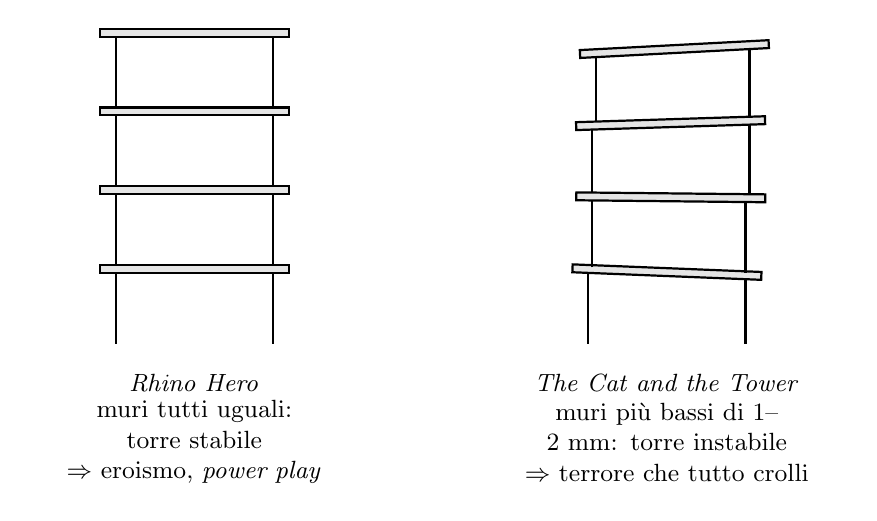
\begin{tikzpicture}[font=\small, x=1cm, y=1cm]
  % Rhino Hero: piani regolari
  \begin{scope}[shift={(0,0)}]
    \foreach \y in {0,1,2,3}{
      \draw[thick] (0,\y) -- (0,\y+0.9);
      \draw[thick] (2,\y) -- (2,\y+0.9);
      \draw[thick, fill=gray!20] (-0.2,\y+0.9) rectangle (2.2,\y+1.0);
    }
    \node[align=center] at (1,-0.5) {\emph{Rhino Hero}};
    \node[align=center, text width=4cm] at (1,-1.25)
      {muri tutti uguali: torre stabile\\$\Rightarrow$ eroismo, \emph{power play}};
  \end{scope}
  % Cat and Tower: muri di altezze diverse
  \begin{scope}[shift={(6,0)}]
    \draw[thick] (0,0) -- (0,0.9);   \draw[thick] (2,0) -- (2,0.82);
    \draw[thick, fill=gray!20, rotate around={-2.3:(0,0.9)}] (-0.2,0.9) rectangle (2.2,1.0);
    \draw[thick] (0.05,0.97) -- (0.05,1.82); \draw[thick] (2.0,0.9) -- (2.0,1.8);
    \draw[thick, fill=gray!20, rotate around={-0.6:(0.05,1.82)}] (-0.15,1.82) rectangle (2.25,1.92);
    \draw[thick] (0.05,1.92) -- (0.05,2.72); \draw[thick] (2.05,1.9) -- (2.05,2.78);
    \draw[thick, fill=gray!20, rotate around={1.8:(0.05,2.72)}] (-0.15,2.72) rectangle (2.25,2.82);
    \draw[thick] (0.1,2.82) -- (0.1,3.64); \draw[thick] (2.05,2.88) -- (2.05,3.78);
    \draw[thick, fill=gray!20, rotate around={3.0:(0.1,3.64)}] (-0.1,3.64) rectangle (2.3,3.74);
    \node[align=center] at (1,-0.5) {\emph{The Cat and the Tower}};
    \node[align=center, text width=4.4cm] at (1,-1.25)
      {muri più bassi di 1--2 mm: torre instabile\\$\Rightarrow$ terrore che tutto
      crolli};
  \end{scope}
\end{tikzpicture}
\caption{Stessa meccanica, paragame diverso: due torri di cartone. In \emph{Rhino Hero}
i piani sono regolari e la dinamica è quella dell'eroe che sale; in \emph{The Cat and
the Tower} alcuni muri sono di uno o due millimetri più bassi, e la torre, sempre
storta, trasmette paura e fragilità. Schema illustrativo, con le pendenze esagerate.}
\label{a10:fig:torri}
\end{figure}

% ---------------------------------------------------------------------
\section{Chiusura: ci si vede il 12}
\label{a10:sec:chiusura}

Mancano tre minuti, ``tempo per un'ultima domanda'', magari ``quella nell'angolino, un
po' timida''. Non arriva (``adesso non ce la faccio''). Gianmarco si smuta, ``il segnale
internazionale'' di chi sta per salutare, ma non ha domande; Ruggero lo invita
scherzosamente a dire anche solo ``cose stupide, tipo: oggi ho ucciso una mosca in
bagno''.

``Allora, gente, io vi saluto, e la lezione di oggi si conclude così.'' L'appuntamento è
\textbf{il 12}, con i \emph{pitch}: ``non fate scherzi, so che li avete, so che li potete
fare''. Al \emph{pitch} non ci sarà solo Ruggero: ci saranno anche \textbf{Beatrice} e
\textbf{Daniele}. ``Buona serata, buona cena, buon weekend.''

% ---------------------------------------------------------------------
\section*{Punti chiave del capitolo}
\addcontentsline{toc}{section}{Punti chiave del capitolo}

\begin{itemize}
  \item La \textbf{UX} è un primo strato tra la persona che si avvicina al gioco e
        l'ecosistema di regole: può essere ``un incredibile aiuto o un gigantesco
        ostacolo''. Regole perfette che non arrivano a chi gioca finiscono ``nel
        cestino''.
  \item I \textbf{quattro pilastri}: \textbf{immediatezza} (si capisce subito, senza
        sforzo: spade e scudi, il barile di petrolio, l'alloro dei punti vittoria),
        \textbf{efficienza} (un'azione complessa nel minor spazio: ``pesca una carta''),
        \textbf{memorabilità} (il +4 di \emph{Uno}, il simbolo di ``tappare'' di
        \emph{Magic}), \textbf{soddisfazione} (\emph{Parks}, \emph{Canvas}, \emph{Tiny
        Epic Mechs}). Sono indipendenti: le icone di \emph{Race for the Galaxy} sono poco
        immediate ma molto efficienti.
  \item Immediato per chi gioca abitualmente non vuol dire immediato per tutti; anche il
        \textbf{colore} fa parte del significato di un'icona.
  \item Il \textbf{wireframe} delle carte cambia durante il prototipo: togliere ciò che
        vale zero, ridurre il testo con le icone, spostare ciò che conta meno. Nei primi
        stadi: \textbf{carte funzionali, non carte belle}.
  \item \textbf{Accessibilità}: font per la dislessia, \emph{curb cut effect} (ciò che è
        più accessibile per qualcuno lo è per tutti), daltonismo da verificare con
        \textbf{Chromatic Vision Simulator}; i mancini e le carte a ventaglio.
  \item Il \textbf{paragame} estende al gioco il \textbf{paratesto}: tutto ciò che non è
        regole e non è fiction, ma incide sull'esperienza. I bordi sono zone grigie
        (i librogame, \emph{Lift It}).
  \item Le aree: \textbf{materialità} (legno, plastica, metallo, app, spessore e
        \emph{core} delle carte, \emph{standee}; clessidra contro timer),
        \textbf{formato} (font, misura delle carte, \emph{200 Word RPG}),
        \textbf{regolamento} (pagine, più libretti, video, glossario,
        \emph{playthrough}, \emph{play aid}), \textbf{scatola} (dall'armadio alla
        Kallax), \textbf{grafica e illustrazioni} (due mestieri diversi),
        \textbf{interfaccia analogica}, \textbf{ambiente} (il tavolo IKEA, il treno,
        \emph{Jenga} in aereo), \textbf{audio}, \textbf{contesto}, \textbf{lingua},
        \textbf{spazio urbano e ibridi digitali}, \textbf{inserti e setup}.
  \item Il paragame \textbf{incide sulle regole}: il formato limita la complessità
        delle regole, la clessidra cambia la tensione, la colonna sonora può essere una
        meccanica. Ai \emph{pitch} e alle revisioni Ruggero chiederà
        \textbf{``tantissimi perché''}.
  \item I casi studio vanno da \emph{Cuba Libre} (due regolamenti, diagrammi di flusso
        per i bot, brochure per fazione) a \emph{193 Days} (solo un mazzo), da
        \emph{Shenzhen I/O} (il manuale stampato) a \emph{Meltdown} (tessere di
        ghiaccio). Il test: ``\textbf{poteva essere di cartone?}''
  \item Il paragame non agisce direttamente sulle dinamiche: agisce sulle meccaniche
        (e sulla fiction), come tutto il design. Serve a far sì che \textbf{le intenzioni
        di design arrivino} a chi gioca, anche quando chi l'ha progettato non è al
        tavolo.
  \item Gli \textbf{inserti} non sono un dettaglio: nessuno ama il \emph{setup}, e un
        buon inserto lo accorcia. Il \emph{setup} si può anche rendere parte del gioco,
        nei giochi leggeri.
  \item \textbf{Ricerca e sviluppo} anche sul paragame: \emph{Rhino Hero} e \emph{The
        Cat and the Tower} hanno la stessa meccanica, ma muri di altezza diversa
        trasformano l'eroismo in terrore. \emph{Copy, transform, combine}, e
        \textbf{cross-modalità}.
\end{itemize}

%    % =====================================================================
%  Analog Game Design, lezione 11 — Il pitch dei progetti di gruppo.
%  Una lezione senza slide e senza lezione frontale: i tre gruppi del
%  corso presentano in tre minuti l'idea del gioco che svilupperanno
%  fino a dicembre, e i tre docenti (Daniele, Beatrice e Ruggero) fanno
%  domande, si ritirano a discutere in privato e poi restituiscono i
%  feedback. In apertura, l'attesa e le regole del pitch. Poi i tre
%  pitch, ciascuno con le sue domande: Murder Memory (escape room
%  investigativa da tavolo a squadre), La Peste (party game a ruoli
%  segreti ispirato alla Maschera della Morte Rossa), un gioco di ruolo
%  in solitario deck building, roguelike e journaling. Dopo la camera
%  di consiglio: la premessa ai feedback (indicazioni, non consigli; il
%  regolamento di massima per il 6 novembre), la domanda di Tiziana su
%  che cosa sia un regolamento in una escape room, i feedback gruppo
%  per gruppo con i casi studio assegnati, il legame tra obiettivo e
%  agency, il perché dei tre minuti, i giochi "generalisti". Infine le
%  domande aperte: scrivere il gioco per chi lo gioca senza di voi, la
%  curse of knowledge, la vergogna delle idee, e una lunga discussione
%  su roguelike, RNG e narrativa modulare (partire dalle emozioni, non
%  dai perk; le meccaniche come metafore; l'ortogonalità).
%  Fonte: trascrizione dell'undicesima lezione (AGD11) del corso breve
%  di Analog Game Design, seconda edizione: una lezione online di circa
%  tre ore, lunedì 12 ottobre 2026, condotta da Daniele con Beatrice e
%  Ruggero.
%  Pacchetti richiesti nel preambolo del libro (già presenti nel
%  main.tex): \usepackage{booktabs}, \usepackage{tikz} con
%    \usetikzlibrary{shapes.geometric,shapes.symbols,shapes.misc,
%      arrows.meta,positioning,calc,fit}
%  (le librerie vanno caricate nel preambolo, non nel capitolo).
%  Consigliati, come per gli altri capitoli: \usepackage[italian]{babel}
%  e \usepackage[T1]{fontenc} (il capitolo compila anche senza).
%
%  Collocazione nel libro: parte "Analog Game Design", undicesimo
%  capitolo (numerazione propria 2.11). Nel file principale del libro,
%  subito dopo il capitolo 2.10:
%
%    % =====================================================================
%  Analog Game Design, lezione 10 — UX design e paragame. In apertura,
%  l'attesa (le lezioni con Beatrice, i gruppi che cambiano idea a pochi
%  giorni dal pitch) e due domande su Tabletop Simulator (prendere un
%  mazzo intero, simulare le luci con gli script); poi la prima parte,
%  sulla UX del gioco: la UX come strato tra chi gioca e l'ecosistema di
%  regole, i quattro pilastri (immediatezza, efficienza, memorabilità,
%  soddisfazione) con i loro esempi di icone e componenti, quante
%  informazioni porta una carta, il wireframe che cambia durante la
%  prototipazione, l'accessibilità (font per la dislessia, curb cut
%  effect, daltonismo). Dopo la pausa, la seconda parte, sul paragame:
%  l'esercizio del libro consigliato, dal paratesto al paragioco, e le
%  aree progettabili (materialità, formato, regolamento, scatola,
%  grafica e illustrazioni, interfaccia analogica, ambiente, audio,
%  contesto, lingua, spazio urbano e ibridi digitali). Dopo la seconda
%  pausa, una lunga serie di casi studio (da Cuba Libre a Meltdown) e
%  la mezz'ora di discussione aperta: il font di Al Rashid, paragame e
%  dinamiche, graphic design contro illustrazione, gli inserti e il
%  setup, chi pensa al paragame in un progetto vero (Rhino Hero e The
%  Cat and the Tower).
%  Fonte: trascrizione della decima lezione (AGD10) del corso breve di
%  Analog Game Design, seconda edizione: una lezione online di circa
%  tre ore, condotta da Ruggero, con due pause (fino alle 18:00 circa e
%  dalle 18:57 alle 19:05).
%  Pacchetti richiesti nel preambolo del libro (già presenti nel
%  main.tex): \usepackage{booktabs}, \usepackage{tikz} con
%    \usetikzlibrary{shapes.geometric,shapes.symbols,shapes.misc,
%      arrows.meta,positioning,calc,fit}
%  (le librerie vanno caricate nel preambolo, non nel capitolo).
%  Consigliati, come per gli altri capitoli: \usepackage[italian]{babel}
%  e \usepackage[T1]{fontenc} (il capitolo compila anche senza).
%
%  Collocazione nel libro: parte "Analog Game Design", decimo capitolo
%  (numerazione propria 2.10). Nel file principale del libro, subito
%  dopo il capitolo 2.9:
%
%    \input{AGD/AGD9_project_management_e_giochi_formativi}
%    \input{AGD/AGD10_ux_design_e_paragame}
%
%  Tutte le etichette di questo capitolo hanno il prefisso "a10:"
%  (a10:cap:..., a10:sec:..., a10:fig:..., a10:tab:...). Il capitolo è
%  autonomo: non contiene \ref verso altri capitoli.
%  Le figure e le tabelle sono ricostruzioni schematiche di quanto il
%  docente spiega a voce e mostra con le slide, non copie delle slide.
%  Dove la trascrizione è troppo rovinata per ricostruire un dettaglio
%  (un nome di gioco, una misura), il capitolo lo dice invece di
%  inventarlo.
% =====================================================================

\chapter[UX design e paragame]{UX design e paragame: l'interfaccia del gioco e
tutto ciò che non è né regole né fiction}
\label{a10:cap:paragame}

Questa è la \textbf{decima lezione} del corso di \textbf{Analog Game Design}, e
l'ultima prima del \emph{pitch} del 12 ottobre. Il suo tema è annunciato da Ruggero
già nei primi minuti, con un entusiasmo che non nasconde: ``oggi, lezione sul
paragioco. Quindi, sono carichissimo''. La lezione ha due metà. La prima è dedicata
alla \textbf{UX} (\emph{user experience}) del gioco, ``una roba gigantesca'' che non
riguarda solo il gioco analogico ma tutti i campi del design, e di cui il corso dà
solo le basi: che cosa sta tra la persona che si siede al tavolo e l'ecosistema di
regole, e quali sono i \textbf{quattro pilastri} di una buona UX
(\textbf{immediatezza}, \textbf{efficienza}, \textbf{memorabilità},
\textbf{soddisfazione}), mostrati con decine di icone e componenti di giochi veri, più
o meno riusciti. Chiude la prima metà una parte sull'\textbf{accessibilità}. Ruggero
la presenta come la parte di ``cose che magari già sapete''.

La seconda metà, sul \textbf{paragame} (o \emph{paragioco}), è invece ``una delle mie
parti preferite'', e ``sempre una parte delle lezioni abbastanza che spacca i
cervelli''. Il paragame è l'estensione al gioco del concetto letterario di
\emph{paratesto}: tutto ciò che di un gioco \textbf{non è regole e non è fiction}, ma
incide sull'esperienza di chi gioca. Il materiale dei dadi, lo spessore delle carte,
il numero di pagine del regolamento, la forma della scatola, il font, il tavolo su cui
il gioco verrà apparecchiato, la musica, il contesto culturale, la lingua, la città.
Dopo una carrellata delle aree progettabili, Ruggero mostra una lunga serie di
\textbf{casi studio}, ``da giochi più regolari a cose più \emph{deranged}'': un
wargame con sei brochure, un gioco di ruolo fatto solo di un mazzo di carte, un
videogioco che chiede di stampare un manuale, una gru da mettersi in testa, delle
tessere di ghiaccio da tenere in freezer. Il messaggio di fondo è uno, e Ruggero lo
ripete in molte forme: niente di tutto questo è ``contorno''. Il paragame
\textbf{incide sulle regole} e sull'esperienza, e chi progetta ``può lavorarci
attorno'' solo se ci ragiona. Per questo, ai \emph{pitch} e alle revisioni, il
docente chiederà ``tantissimi perché''.

La lezione è \textbf{online} e la conduce da solo \textbf{Ruggero}, condividendo le
slide. Si colloca con ogni probabilità \textbf{venerdì 9 ottobre 2026}\footnote{La
data non è detta, ma è ricostruibile. Nella lezione su Tabletop Simulator Ruggero
aveva indicato venerdì 9 ottobre come la data della lezione sul paragame. In questa
lezione dice che il \emph{pitch} ``del 12'' è ``lunedì'', e in chiusura gli studenti
si salutano con ``buon weekend''.}, dalle 17 alle 20 circa. Ci sono due pause: la
prima, di dieci minuti, alla fine della parte sulla UX (``alle sei ci ritroviamo
qua''); la seconda dalle \textbf{18:57} alle \textbf{19:05} (``ve ne do 8 per il numero
tondo''), prima dei casi studio. All'inizio sono collegati, tra gli altri,
\textbf{Tancredi} e \textbf{Gianmarco}; nel corso della lezione intervengono anche
\textbf{Tiziana} e \textbf{Lorenzo}\footnote{La trascrizione non distingue tra i due
Lorenzo del corso (Lorenzo Vergata e ``l'altro Lorenzo''); in un passaggio Ruggero
chiama ``Tancredi, Lorenzo. Lorenzo'', il che fa pensare che siano presenti
entrambi. Il capitolo scrive semplicemente ``Lorenzo''.}. Tiziana lascia la lezione
verso la fine (``Ciao, Tiziana'').

Tre avvertenze di lettura, le stesse dei capitoli precedenti. La prima: la
trascrizione è automatica e storpia moltissimi nomi, a cominciare da quelli dei due
argomenti della lezione. La UX diventa ``Wix'', ``l'usso'' e ``Wix design''; il
paragame diventa ``paragain'', ``paraghino'', ``paraggio'', ``parachain'',
``paragate'', ``paradigma'', ``paracadema'' e perfino ``guerra game''. \emph{Race for
the Galaxy}, il gioco più citato della serata, è ``Restore the Galaxy'', ``Rescord
Galaxy'', ``RIS4D Galaxy'', ``Risordiality'', ``Redsward Galaxy'', ``Days for the
Galaxy'' e ``Risk for the Gala''. Dove la ricostruzione è sicura, o molto probabile, il
capitolo usa la forma corretta e lo segnala in nota la prima volta; dove non lo è,
riporta la forma della trascrizione e lo dice. La seconda: durante le due pause la
trascrizione registra per decine di righe frasi senza alcun rapporto con la lezione,
ripetute in loop (``grazie a tutti per l'attenzione che ci ha spiegato'', ``qual è la
risposta che ci può essere?''), e subito dopo la seconda pausa qualche frase spuria
(``la situazione di oggi è la migliore dal 2000'', ``otto orecchie''). Sono artefatti
del riconoscimento vocale e il capitolo le ignora. La terza: gli studenti intervengono
spesso senza che la trascrizione segnali chi parla; il capitolo li nomina quando il
contesto lo rende chiaro e resta generico altrimenti.

\paragraph{Come leggere questo capitolo.} La lezione è costruita quasi interamente
su \textbf{immagini}: icone, carte, scatole, componenti, foto di giochi apparecchiati.
Nessuna di queste immagini è nella trascrizione. Il capitolo ricostruisce ciò che
Ruggero ne dice e, dove serve, descrive l'immagine a parole; quando un dettaglio
dell'immagine non è ricostruibile, lo segnala. Le tabelle riassumono le liste (i
quattro pilastri, le aree del paragame, i casi studio); le figure ricostruiscono gli
schemi (il posto della UX tra la persona e il gioco, le tre aree sovrapposte di
regole, fiction e paragame, il ventaglio di carte in mano). Le slide della lezione,
dice Ruggero, sono già nella cartella condivisa del corso. Qua e là, dei paragrafi di
\textbf{approfondimento} collegano la lezione ai libri di game design di riferimento
(soprattutto \emph{The Art of Game Design} di Jesse Schell) e alla letteratura sul
design dell'interazione e sul paratesto; sono segnalati come tali e non fanno parte
della lezione.

Il percorso del capitolo segue quello della lezione:
\begin{enumerate}
  \item l'attesa e due domande su Tabletop Simulator (sezioni \ref{a10:sec:attesa}
        e~\ref{a10:sec:tts});
  \item la \textbf{UX del gioco}: il suo posto nella \emph{pipeline} e i
        \textbf{quattro pilastri}, ciascuno con i suoi esempi (sezioni
        da~\ref{a10:sec:ux} a~\ref{a10:sec:soddisfazione});
  \item quante informazioni contiene una carta, il \textbf{wireframe} che cambia
        nel prototipo, l'\textbf{accessibilità} (sezioni da~\ref{a10:sec:informazioni}
        a~\ref{a10:sec:accessibilita});
  \item dopo la prima pausa, l'esercizio del \textbf{libro consigliato} e la
        definizione di \textbf{paragame} (sezioni \ref{a10:sec:libro}
        e~\ref{a10:sec:definizione});
  \item le \textbf{aree progettabili} del paragame, una per una (sezioni
        da~\ref{a10:sec:aree} a~\ref{a10:sec:pervasivo});
  \item dopo la seconda pausa, i \textbf{casi studio} (sezione~\ref{a10:sec:casi});
  \item la \textbf{discussione aperta} e la chiusura (sezioni
        da~\ref{a10:sec:discussione} a~\ref{a10:sec:chiusura}).
\end{enumerate}

% ---------------------------------------------------------------------
\section{L'attesa: il 12 ``sta nella pietra''}
\label{a10:sec:attesa}

Ruggero si collega con qualche minuto di ritardo (``pensavo di essere in ritardo'':
c'è stato un cambio di aula, ``ma siamo in orario''), e il clima è quello di fine
settimana. Si parla del caldo (``fa ancora troppo caldo per i miei gusti''), poi
Ruggero chiede come siano andate le lezioni con Beatrice (``interessante'',
``bene'') e come procedano i progetti di gruppo. Arrivano alla spicciolata gli
studenti del \textbf{gruppo 2}, che hanno appena fatto ``un piccolo meeting'' e
raccontano di aver \textbf{cambiato completamente} l'idea proposta. Ruggero non si
scompone: ``è normale''. C'è tempo fino al 12, ``però il 12 sta nella pietra''. Uno
studente, appena entrato, ammette di essere ``un po' incasinato col gioco'', e la
risposta è la stessa: ``ma è normale''. Quando qualcuno, scherzando, teme che al
\emph{pitch} i docenti ``sfasceranno'' le idee dei gruppi, Ruggero rassicura: ``no, non
vi sfasciamo niente''.

Ruggero aggiunge una promessa che riguarda direttamente il \emph{pitch}: la lezione
di oggi è ``proprio fatta apposta'' per chi ha ancora ``qualche buco di dubbio''. In
particolare la seconda parte darà ``delle idee intense'', che ``potrebbero portarvi a
riparlare tra di voi di varie cose in gruppo''; ed è sicuro che ``questo porterà lunedì
ad avere dei \emph{pitch} incredibili''.

Come al solito, prima di cominciare apre lo spazio per ``domande, dubbi, consigli,
insulti'', ``altrimenti stiamo qui in silenzio a osservare lo scorrere del tempo, e lo
sapete che non fa piacere a nessuno''. E annuncia il tema: ``UX design e paragame''.
Sulla prima parte, ``molte persone tra voi già sono sul pezzo'', perché la UX ``non è
una cosa esclusiva del gioco da tavolo'' ma tocca tutti i campi del design; la seconda,
invece, nelle edizioni passate è ``sempre una parte delle lezioni abbastanza che spacca
i cervelli. Quindi, non vedo l'ora''.

% ---------------------------------------------------------------------
\section{Due domande su Tabletop Simulator}
\label{a10:sec:tts}

Una studentessa ne approfitta per due domande ``molto semplici'' su Tabletop
Simulator, il software della lezione precedente\footnote{La trascrizione non dice chi
fa le domande; dal contesto è una persona che sta lavorando a un gioco ``per conto
mio'', fuori dal progetto di gruppo.}.

\paragraph{Prendere un mazzo intero senza tenere premuto.} La prima domanda riguarda
un fastidio pratico: per prendere un mazzo di carte intero, e non una carta sola,
bisogna tenere premuto il tasto del mouse per un paio di secondi. C'è una scorciatoia?
Ruggero ricorda prima quella per \textbf{pescare}: basta passare col mouse sopra il
mazzo e, senza cliccare, premere sulla tastiera il \textbf{numero} di carte da pescare
(``premo 5 e mi dà 5 carte in mano''). Ma la studentessa vuole \emph{spostare} il mazzo
intero, e le capita spesso. ``Che io sappia, bisogna tenere premuto'', risponde
Ruggero, che non ne ha mai avuto bisogno: se capita spesso, forse è ``più un problema
di logistica di come il modulo è \emph{set up}'', e si risolve ``setappando il modulo
bene''. Forse esiste un ``control-click'', ``non credo ci sia, ma chi può dirlo. Se lo
scopri, dimmelo''.

\paragraph{Simulare le luci.} La seconda domanda riguarda il gioco a cui la
studentessa lavora: un gioco con un \textbf{lumino} che proietta un'ombra, giocato
``tutto al buio''. Su Tabletop Simulator ha visto un modulo che simula le luci: si può
fare? ``Serve script? Assolutamente, per forza.'' E Ruggero sconsiglia ``fortemente''
di testare su TTS cose che lo richiedono: lì ``si apre il vaso di Pandora degli
script'', una cosa impegnativa che il corso non copre perché usa \textbf{Lua} come
linguaggio di programmazione, e fare ``delle lezioni di Lua apposta per dei casi
limite'' non ha senso nel programma. La studentessa chiede se basti copiare l'asset di
quel modulo. ``Puoi copiare l'asset se lo salvi'', ma dipende da come è stato
costruito. Se chi l'ha creato è stato ``furbo'', lo script è dentro l'asset stesso; ma
a Ruggero è capitato di trovare moduli con \textbf{script diffusi}, in parte in un
componente e in parte in un altro: se se ne copia uno solo, ``si rompe tutto e non
funziona''. Ruggero non conosce quel modulo: ``poi fare un po' di prove, sicuramente''.

\paragraph{Approfondimento: perché il gioco ``al buio'' è un tema di questa lezione.}
La domanda è più vicina all'argomento della serata di quanto sembri. Un lumino che
proietta ombre su un tavolo buio è un elemento di \emph{paragame} (luce, materiali,
ambiente) che diventa una meccanica: proprio il tipo di intreccio che Ruggero mostrerà
con \emph{Nyctophobia}, \emph{Scandal in the Deep} e \emph{Meltdown}
(sezione~\ref{a10:sec:casi}). Ed è anche un buon esempio del limite pratico del
prototipo digitale: ciò che dipende dalla fisica e dalla percezione (la luce, il peso,
la temperatura) si simula male in un software, e va provato sul tavolo vero.

% ---------------------------------------------------------------------
\section{La UX nel gioco: uno strato tra la persona e le regole}
\label{a10:sec:ux}

Ruggero condivide lo schermo e apre le slide: ``UX design e paragame'', una lezione
``divisa più o meno in due'', con ``una pausa a metà'' (``non sarà tutta una
mitragliata secca di cose''). La seconda parte sarà ``contemporaneamente un po' più
intensa, ma anche un po' più \emph{relaxed} della prima. Lo so, mi direte: com'è
possibile? Lo vedrete''.

Si parte dalla UX, con una premessa: è ``una roba gigantesca'' e ``questo non è un
corso di UX design''; la lezione si limita a dare ``delle basi su cui ragionare''. Gli
esempi saranno quasi tutti di \textbf{giochi da tavolo}, e non per caso: è un genere
che, più di altri, ``ha richiesto in passato un uso della UX fatto meglio'' rispetto,
per esempio, a un gioco di ruolo, o a un LARP in cui ``non è detto che venga neanche
usato il materiale stampato''.

\subsection{Dove sta la UX}

Il punto di partenza è una \emph{pipeline} che la classe ``dovrebbe già sapere'': una
\textbf{persona} che vuole giocare, il \textbf{gioco} (l'ecosistema di regole) e
l'\textbf{esperienza} che ne nasce. Il lavoro della UX ``sta qua in mezzo'': è ``un
primo \emph{layer} tra la persona che si approccia al gioco e l'ecosistema di regole
del gioco'' (figura~\ref{a10:fig:pipeline}). E ``spesso non ci si pensa, ma può essere
un incredibile aiuto o un gigantesco ostacolo''. Si può avere un ecosistema di regole
``lisciissimo, pulitissimo, fantastico'', in cui ``funziona tutto, bilanciato tutto'';
``ma se a livello di interfaccia questa roba non arriva, non si riesce a giocare, non si
riesce neanche a capire come giocare. Quel gioco finisce nel cestino''.

Di qui la regola: quando si progetta un gioco ``non ragioniamo solo alle meccaniche
del gioco, ma anche a cosa c'è davanti al gioco''. Che cosa c'è ``prima ancora delle
questioni di meccaniche, delle regole, ma anche prima del manuale'': il regolamento in
quanto oggetto, ``come sono fatte le carte, come il gioco è apparecchiato sul
tavolo''.

\begin{figure}[htbp]
\centering
\begin{tikzpicture}[
  font=\small,
  box/.style={draw, thick, rounded corners=3pt, minimum height=1.1cm,
              text width=2.5cm, align=center},
  ux/.style={draw, thick, dashed, rounded corners=3pt, fill=gray!15,
             minimum height=1.6cm, text width=2.6cm, align=center},
  arr/.style={-{Stealth[length=3mm]}, thick}
]
  \node[box] (p) {\textbf{Persona}\\che vuole giocare};
  \node[ux, right=0.9cm of p] (u) {\textbf{UX}\\icone, carte, regolamento,
    tavolo apparecchiato};
  \node[box, right=0.9cm of u] (g) {\textbf{Gioco}\\ecosistema di regole};
  \node[box, right=0.9cm of g] (e) {\textbf{Esperienza}};
  \draw[arr] (p) -- (u);
  \draw[arr] (u) -- (g);
  \draw[arr] (g) -- (e);
  \node[below=0.35cm of u, text width=3.4cm, align=center, font=\footnotesize]
    {``un incredibile aiuto\\o un gigantesco ostacolo''};
\end{tikzpicture}
\caption{Il posto della UX nella \emph{pipeline} persona--gioco--esperienza: un primo
strato tra chi si avvicina al gioco e l'ecosistema di regole. Se questo strato non
funziona, anche regole perfette non arrivano a chi gioca.}
\label{a10:fig:pipeline}
\end{figure}

\subsection{I quattro pilastri}
\label{a10:sec:pilastri}

Per progettare la UX di un gioco, Ruggero dà ``quattro pilastri che è bene tenere a
mente'': una buona UX ha \textbf{immediatezza}, \textbf{efficienza},
\textbf{memorabilità} e \textbf{soddisfazione} (tabella~\ref{a10:tab:pilastri}). Le
sezioni che seguono li vedono uno alla volta, ``nel dettaglio'', con esempi presi da
giochi reali. Una precisazione vale per tutti gli esempi: ``non vi serve sapere questi
giochi da dove arrivano''. Anzi, per alcune domande è meglio non conoscerli.

\begin{table}[htbp]
\centering
\small
\begin{tabular}{@{}p{2.6cm}p{5.4cm}p{5.2cm}@{}}
\toprule
\textbf{Pilastro} & \textbf{Che cosa vuol dire} & \textbf{Esempi della lezione} \\
\midrule
Immediatezza & si capisce subito il significato, con il minimo sforzo e senza
confusione & spade e scudi sui dadi; il barile di petrolio; la corona d'alloro dei
punti vittoria. Contro-esempi: \emph{Race for the Galaxy}, \emph{Argent} \\
Efficienza & racchiudere un'azione complessa nel minor spazio possibile & l'icona
``pesca una carta''; l'icona del punto vittoria; le icone di \emph{Race for the
Galaxy} (poco immediate, ma molto efficienti) \\
Memorabilità & restare in mente, così che a distanza di anni si ricordi ancora che
cosa fa & il +4 di \emph{Uno}; il simbolo di ``tappare'' di \emph{Magic}; le icone di
\emph{The Gallerist} \\
Soddisfazione & ``bonus point'': interagire con la grafica e i componenti è piacevole,
gratificante & il tracciato a frecce di \emph{Parks}; le carte trasparenti di
\emph{Canvas}; le armi in miniatura di \emph{Tiny Epic Mechs} \\
\bottomrule
\end{tabular}
\caption{I quattro pilastri di una buona UX secondo Ruggero, con gli esempi mostrati
a lezione.}
\label{a10:tab:pilastri}
\end{table}

% ---------------------------------------------------------------------
\section{Immediatezza}
\label{a10:sec:immediatezza}

Un elemento grafico è \textbf{immediato} quando ``comprendiamo subito il significato
di quello che vuole fare, con il minimo sforzo e senza confusione''. Il contrario è
chiaro: se vediamo una cosa e non capiamo che cosa fa, dobbiamo sforzarci, ci
confonde, ``magari facendoci anche sbagliare le regole'', e allora ``quella roba lì è
da buttare nel cestino''.

\subsection{Un tiro di dadi}

Il primo esempio è un \textbf{tiro di tre dadi} di un gioco che nessuno sa quale sia.
Le facce uscite mostrano \textbf{due spade}, \textbf{uno scudo} e \textbf{un fulmine}.
``Che cosa ci dice questo lancio di dadi?'' Le risposte arrivano subito: ``che siamo
stati fulminati'', poi, più seriamente, ``due attacchi, una difesa, e il fulmine non
saprei''. A livello di \emph{vibes}, è ``un lancio di combattimento, evidentemente'',
``perché ci sono le spade, gli scudi'' (``diciamo, combattimento sotto la pioggia col
fulmine'', scherza Ruggero). E in che tipo di gioco potrebbe stare? Uno studente pensa a
qualcosa come \emph{Civilization}, la conquista di un territorio; un altro a un gioco
fantasy, e cita un titolo che la trascrizione rende ``Cronache di Havel''\footnote{Con
ogni probabilità \emph{Le Cronache di Avel} (\emph{Chronicles of Avel}), gioco fantasy
cooperativo con combattimenti a dadi. Il gioco della slide, invece, non viene
nominato.}.

Il punto è che tutti hanno capito \textbf{immediatamente} che le spade sono attacco e
lo scudo è difesa, e che il tiro è ``più aggressivo che difensivo''; e nessuno sa che
cosa sia il fulmine. ``Ed è sempre così, quando io uso questo esempio.'' Spade e scudi
sono usati ``in talmente tanti giochi'', a livello di \textbf{euristiche personali}, che
si capiscono ``al volo anche se non sapete i dettagli di questo gioco'': non si sa come
funzionano il combattimento, la difesa, la vita, ma si sa che due spade e uno scudo
fanno un tiro aggressivo. Il fulmine, nel gioco, è \textbf{l'attivazione di
un'abilità}, ma è ``un'icona poco adatta a fare questo'', perché nessuno l'ha
riconosciuta come tale. Ed è normale: è molto più difficile trovare un'icona che
rappresenti ``in generale un'abilità, che può essere potenzialmente qualunque cosa'',
mentre spada e scudo sono di fatto delle \textbf{sineddoche}, ``delle metafore, in
questo caso, di \emph{ti sto attaccando} o \emph{mi sto difendendo}''.

\subsection{Quattro risorse}

Il secondo esempio sono le icone di \textbf{quattro risorse}, in alto a destra nella
slide. ``Chi è che sa da quale gioco vengono?'' Nessuno: ``best result'', perché la
domanda ``crolla'' se si conosce già il gioco. Le icone riproducono i segnalini di
legno delle risorse, con il loro colore e la loro forma. Che cosa rappresentano?

Le risposte della classe sono istruttive. Uno studente va ``più sul colore che sulla
forma'': il giallo è il grano, il grigio è la pietra, il marrone ``direi legno''.
\textbf{Tancredi} vede nella quarta, color ottanio, il \textbf{petrolio}, ``perché mi
sembra di qualche gioco che avevo provato''. Tiziana nota che ``la forma è
contraddittoria'', non corrisponde al colore; e una studentessa confessa di vederci
tutt'altro: ``una bara, una lapide, il lumino dove si mette il cero e una colonna che
sorregge'', insomma un cimitero.

Ruggero scioglie l'enigma partendo dalle due più semplici. Il \textbf{legno} ``nessuno
lo sbaglia'': è a forma di tronco tagliato, nei limiti di un piccolo componente. Quella
indicata come pietra è in realtà \textbf{metallo}, ma nel gioco non si confonde: il
gioco è ambientato in un mondo \emph{dieselpunk}\footnote{La trascrizione dice ``in cui
fai è site''. Le quattro risorse descritte (legno, metallo, grano e petrolio) e
l'ambientazione dieselpunk con giganteschi macchinari sono quelle di \emph{Scythe}
(Jamey Stegmaier, 2016), che è quasi certamente il gioco della slide.}, ``hai questi
giganteschi macchinari, per costruirli ti serve metallo'', e quindi quello viene preso
come metallo. Quello giallo confonde sempre chi non conosce il gioco, perché sembra
``un sacchetto di qualcosa di giallo'': le due risposte possibili sono oro o grano, e
qui è \textbf{grano}. E quello in cui ``non ci si sbaglia di solito'' è proprio la
risorsa color ottanio: ``Tancredi l'ha detto giusto, è petrolio'', perché usa ``la
colorazione dell'ottanio, che è il colore che culturalmente noi associamo alla benzina,
al gasolio, al carburante''. È forse l'icona più riconoscibile di tutte, perché è un
\textbf{barile di petrolio}. Il contesto, poi, conta: chi pensasse a un gioco come
\emph{Concordia}, ambientato nel Mediterraneo antico, ``non ha senso che sia petrolio''.

Ne esce un'osservazione in più: \textbf{non è solo la forma}; anche il \textbf{colore}
può essere fondamentale per riconoscere un'icona. ``Se io vi facevo il tronco viola,
non mi avreste detto legno. Se vi facevo il grano rosso, non mi avreste detto grano o
soldi, mi avreste detto qualcos'altro.''

\subsection{La corona d'alloro}

Terza domanda: l'icona in basso a destra, una corona con un \textbf{3}. ``Tre punti
vittoria.'' Perché? ``Perché c'è l'alloro.'' E perché l'alloro significa punti
vittoria? Perché l'alloro è un premio, un riconoscimento; e la \textbf{corona d'alloro}
``si è normalizzata, specialmente nei giochi da tavolo \emph{German}, negli Eurogame,
come simbolo dei punti vittoria''. In centinaia di giochi la coroncina d'alloro
rappresenta i punti, e chi trova un gioco con una corona d'alloro e un 3 sa che sono tre
punti.

Qui Ruggero fa una distinzione importante: \textbf{immediato non vuol dire immediato
per chi non ha mai giocato}, ``a tutte le persone''. L'alloro è immediato per chi gioca
abitualmente a giochi da tavolo, perché fa parte di un linguaggio condiviso. Poi,
``chiaramente, la forza di un'icona forte è essere immediata anche per chi non ha
giocato il gioco''.

\subsection{Le icone che fanno il contrario}

Ci sono però icone che fanno ``il contrario di quello che si dovrebbe fare di solito''.
Le prime due della slide, ``che ci crediate o no, sono due icone diverse
meccanicamente, che fanno due cose diverse''. Ruggero non dice che cosa fanno (``ho una
sanità mentale da risparmiarmi''): vengono da un gioco che la trascrizione chiama
``Gemoni''\footnote{Il titolo non è ricostruibile con sicurezza dalla trascrizione.},
``bel gioco'', ma con ``molte icone molto simili'', come queste due, che hanno i colori
praticamente invertiti e fanno cose diverse.

Poi due icone di \textbf{\emph{Race for the Galaxy}}\footnote{La trascrizione lo
storpia in quasi ogni occorrenza: ``Retribuzione'', ``Restore the Galaxy'', ``Rescord
Galaxy'', ``RIS4D Galaxy'', ``Risordiality'', ``Redsward Galaxy'', ``Days for the
Galaxy'', ``Risk for the Gala''. \emph{Race for the Galaxy} (Thomas Lehmann, 2007) è un
gioco di carte di fantascienza celebre per la sua iconografia densa.}. Gianmarco, che
lo conosce, viene escluso dalla domanda (``non lo chiederò a te, perché \emph{Race for
the Galaxy} è una maledizione''). Il gioco ha questa proprietà: ``per chi non lo
conosce, guarda le icone e pensa: questi sono pazzi, questo gioco non ha senso. Per
chi lo conosce, queste icone sono le più leggibili del mondo ed è immediato capire che
cosa fanno''. Ruggero prova a far indovinare la classe (``non do voti
all'interrogazione sulle icone di \emph{Race for the Galaxy}, anche perché sarebbe un
disastro per chiunque, \emph{me included}''), con un suggerimento: è un gioco
fantascientifico.

Sulla prima icona, Lorenzo prova ``annulla un comando'' (``ti sorprenderà sapere che
non è così''), un altro ``cambio colore'' (``ti piacerebbe; non è un gioco facile come
\emph{Uno}, questo''). Poi una studentessa tenta un'``archeologia ludica'': se ci sono
carte di vari colori, forse scartando una carta di quel colore succede qualcosa da
qualche altra parte. ``Un terzo l'hai beccata.'' Gianmarco completa: \textbf{scarti una
carta e la usi come risorsa} da mettere su un \textbf{pianeta}, ``che è quella cosa
tonda''.

``Adesso che abbiamo decifrato parte del linguaggio'', la seconda icona riesce meglio.
Uno studente: ``se hai tre carte blu, ottieni un esagono che non so cosa sia, e peschi
una carta?'' ``Vicinissimo, non sai quanto.'' L'icona parla di carte blu, ma non di
carte qualsiasi: di carte \textbf{usate come risorsa blu}, quelle appena viste. E non ne
servono tre: il numero dice che si può fare \textbf{fino a tre volte} la cosa che
segue, cioè ottenere un \textbf{esagono} (i punti, in questo gioco) e pescare una
carta. Tradotto: ``posso usare da una a tre risorse per prendere da uno a tre punti e
da una a tre carte''.

Infine l'icona in basso al centro, che Ruggero non spiega: ``è un'icona per cui
dovrebbero arrestare i graphic designer immediatamente''. Contiene, ``se non vado
errato'', una specie di \textbf{talismano} di carta scritta, uno \textbf{scudo} e
\textbf{due cappelli}, di cui uno in ombra. Viene da \textbf{\emph{Argent}}\footnote{
\emph{Argent: The Consortium} (Trey Chambers, 2015), gioco di piazzamento lavoratori
ambientato in un'università di magia.}: ``gioco bellissimo, icona illegale''. Che non
sia immediata, ``vi rendete conto anche voi''.

\paragraph{Approfondimento: convenzioni, affordance e linguaggi appresi.} Gli esempi
di Ruggero corrispondono a una distinzione classica del design dell'interazione. Alcuni
segni funzionano perché si appoggiano a \textbf{convenzioni} culturali molto diffuse
(la spada per l'attacco, il colore ottanio per il carburante, l'alloro per la vittoria);
altri richiedono di imparare un \textbf{linguaggio} specifico del singolo gioco, come le
icone di \emph{Race for the Galaxy}. Donald Norman, in \emph{The Design of Everyday
Things}, parla di \emph{significanti} (\emph{signifiers}) per indicare i segni che
comunicano che cosa si può fare con un oggetto, e osserva che le convenzioni sono
potenti proprio perché non vanno reimparate a ogni nuovo oggetto. Il limite che Ruggero
indica (immediato ``per chi gioca'' non è immediato ``per tutti'') è lo stesso: una
convenzione vale solo dentro la comunità che la condivide, e un gioco pensato per un
pubblico nuovo non può darla per scontata.

% ---------------------------------------------------------------------
\section{Efficienza}
\label{a10:sec:efficienza}

Il secondo pilastro è l'\textbf{efficienza}: ``comunicare più informazioni insieme,
alleggerendo l'aggregazione di informazioni''. Ruggero la spiega con ``due esempi
diretti''.

\paragraph{Pescare una carta.} La prima icona mostra un mazzo di carte. Che cosa fa?
``Peschi.'' Perché? ``Perché c'è un mazzo di carte.'' Ma Ruggero insiste: che cosa si fa
\emph{fisicamente}, ``a livello di propri atti fisici'', seduti al tavolo, per attivare
questa icona? ``Rivelo la prima carta del mazzo, prendo la prima carta del mazzo, e
poi\dots{} la metto in mano.'' Per chi gioca molto è una cosa semplicissima, ``solo
perché abbiamo giocato tonnellate di giochi''. Ma l'atto in sé è complesso: c'è un
componente che è un mazzo, che contiene tante carte; ne prendo la prima, la sollevo dal
mazzo e la aggiungo alla mia mano, di cui ora fa parte. ``È un'azione complessa, e
un'icona così ci riassume tutto questo processo.''

\paragraph{Il punto vittoria.} Lo stesso vale per l'icona del punto vittoria vista
prima. Che cosa si fa con un punto vittoria? ``Muoviamo la pedina.'' Se il gioco ha un
tracciato dei punti, quell'icona, ``nella sua piccolezza'', dice: prendi la tua pedina
dei punti vittoria e muovila avanti sul tracciato di tante caselle quanti sono i punti.

``Sono esempi piccoli e banali. Non sottovalutate questa cosa qua.'' Ruggero ne ricava
la definizione: un'icona efficiente \textbf{non} deve essere efficiente per chi non
conosce il gioco; un'icona efficiente ``è in grado di racchiudere al suo interno
un'azione complessa nel minor spazio possibile''. Ecco perché le due icone di \emph{Race
for the Galaxy} sono un caso interessante: sono \textbf{molto poco immediate}, ma
\textbf{molto efficienti}. In uno spazio piccolissimo danno tante informazioni e dicono
molto bene che cosa fare, ``una volta che abbiamo decifrato l'alfabeto di \emph{Race for
the Galaxy}''. I pilastri, insomma, sono indipendenti: un'icona può averne uno senza
l'altro.

% ---------------------------------------------------------------------
\section{Memorabilità}
\label{a10:sec:memorabilita}

Terzo pilastro: una buona icona deve ``rimanere nella mente, in modo da facilitare il
ricordo durante le partite successive''. Il criterio di Ruggero è concreto: ``se io gioco
un gioco e poi lo rigioco cinque anni dopo, e so ancora che cosa fa quell'icona, quello
è un buon gioco''.

\paragraph{Il +4 di \emph{Uno}.} La prima carta della slide: che cosa fa? ``Pescare
quattro carte.'' Chi pesca? Il giocatore successivo. Il gioco è \emph{Uno}. ``E quand'è
che hai giocato l'ultima volta?'' ``Boh. Almeno un paio d'anni fa.'' Non ci si ricorda
nemmeno quando, ma ci si ricorda che cosa fa la carta. Perché è una carta
\textbf{memorabile}: ``quando ti viene giocata contro, bestemmie''. Giocarla, o subirla,
dà ``un \emph{boost} emotivo tale'' che quello che fa diventa memorabile, ``quasi
memetico''.

\paragraph{Il simbolo di ``tappare''.} La seconda icona: dove nasce, che cosa chiede di
fare? Una prima ipotesi (``invertire il turno'') è sbagliata; poi uno studente fa
l'``ipotesi molto scontata'': \textbf{\emph{Magic: The Gathering}}. L'icona chiede di
\textbf{tappare} la carta, cioè di \textbf{ruotarla di 90 gradi}: una carta tappata ha
usato la sua abilità e non la si può riutilizzare nel turno. ``Quand'è l'ultima volta che
hai giocato a \emph{Magic}?'' ``Cent'anni fa.'' Eppure ci si ricorda ancora che quel
simbolo vuol dire ``prendi la carta e ruotala di 90 gradi''. Il motivo, qui, è diverso
da \emph{Uno}: è che il simbolo è \textbf{pervasivo}, ``è ovunque''; chi ha giocato a
\emph{Magic} l'ha incontrato per forza.

\paragraph{Le icone di \emph{The Gallerist}.} Le ultime due icone sono riconosciute da
uno studente, che ricorda il gioco ma non l'effetto: \textbf{\emph{The
Gallerist}}\footnote{\emph{The Gallerist} (Vital Lacerda, 2015), gioco in cui si
gestisce una galleria d'arte.}. La prima dà popolarità, la seconda soldi, in proporzione
ai \emph{meeple} presenti: un punto ogni due \emph{meeple} di un colore (magenta, nel
primo caso; marroni, nel secondo) oppure ogni \emph{meeple} bianco. ``Quindi, se ho
quattro magenta e un bianco prendo tre; se ho otto magenta prendo quattro.'' Chi ha
giocato a \emph{The Gallerist} se le ricorda, perché sono ``dappertutto in tutto il
gioco''. E sono icone che, quando te le spiegano la prima volta, ``vi sparate''; ``ma
dopo il primo turno nessuno va a riguardare nel regolamento che cosa fanno''.

Dai tre esempi escono tre strade diverse verso la memorabilità: l'\textbf{emozione}
(\emph{Uno}), la \textbf{pervasività} di un simbolo in tutto un sistema di gioco
(\emph{Magic}), la \textbf{ripetizione} dentro una singola partita (\emph{The
Gallerist}).

% ---------------------------------------------------------------------
\section{Soddisfazione}
\label{a10:sec:soddisfazione}

``Memorabili, immediate, efficienti: fantastico. Ma \emph{bonus point} se è anche
\textbf{soddisfacente}'': se interagire con l'aspetto grafico, con la UX del gioco, è
piacevole e gratificante. Tre esempi.

\paragraph{Il tracciato di \emph{Parks}.} In \emph{Parks}\footnote{\emph{Parks}
(Henry Audubon, 2019), gioco di escursioni nei parchi nazionali statunitensi.} il
tracciato su cui ci si sposta con i propri pedoncini è composto da \textbf{tessere}, e
ci si muove in una sola direzione, da sinistra verso destra. Le tessere hanno una forma
quasi a \textbf{freccia}, sono ``un po' inclinate in modo che si incastrino'', formando
una specie di nastro che indica la direzione. ``Potevano essere rettangoli? Sì, non
cambia niente meccanicamente.'' Ma incastrarle in ordine, oltre a essere memorabile
(perché ricorda la direzione), è anche ``molto soddisfacente''.

\paragraph{I quadri di \emph{Canvas}.} In \emph{Canvas}\footnote{\emph{Canvas} (Jeff
Chin e Andrew Nerger, 2021).} si compongono dei quadri con delle carte di
\textbf{plastica semitrasparente}: ogni quadro è fatto di \textbf{tre strati}
sovrapposti. Non solo gli elementi si combinano visivamente, ma anche il \textbf{nome
del quadro} viene generato dalle carte giocate: alcune carte danno la prima parte del
nome, altre la seconda.

\paragraph{Le armi di \emph{Tiny Epic Mechs}.} L'ultimo è un gioco di \emph{mech} che
combattono\footnote{La trascrizione dice ``Tiny Pic Max'': è \emph{Tiny Epic Mechs}
(Scott Almes, 2019).}, in cui i \emph{meeple} entrano dentro delle piccole
\textbf{armature di plastica}; e quando si cambia equipaggiamento, si mettono loro in
mano ``le piccole armi e gli scudini''. ``Meccanicamente, non cambia niente'':
l'equipaggiamento è comunicato anche dalle carte. Ma è molto soddisfacente, e ``ci
ricordiamo al volo che cosa abbiamo in mano, perché fisicamente il nostro \emph{meeple}
ce l'ha in mano'': un lanciagranate, uno scudo. E quando si cambia arma, si cambia non
solo la carta, ma anche il pezzettino.

\paragraph{Approfondimento: la soddisfazione come ``feedback'' fisico.} Schell, in
\emph{The Art of Game Design}, dedica all'interfaccia un intero capitolo e insiste su un
punto che questi esempi rendono evidente: un'interfaccia non serve solo a trasmettere
informazioni, ma a dare a chi gioca la sensazione di \textbf{controllo} e un
\textbf{feedback} piacevole a ogni azione. Nel videogioco si parla di \emph{juiciness},
la ``succosità'' delle reazioni alle azioni del giocatore; nel gioco analogico lo stesso
ruolo è svolto dal gesto fisico: l'incastro di una tessera, la sovrapposizione di un
foglio trasparente, l'arma infilata nella mano di una miniatura.

% ---------------------------------------------------------------------
\section{Quante informazioni porta una carta?}
\label{a10:sec:informazioni}

Dopo una breve verifica (``stiamo andando lisci''), Ruggero pone una ``domanda da
tenere conto sulla UX'': \textbf{quante informazioni stiamo usando?}

Sulla slide ci sono due carte di due giochi di carte di fantascienza con un tema molto
simile, la colonizzazione interplanetaria. Una è ancora di \emph{Race for the Galaxy}:
``pensavate che fosse brutta solo l'icona. E invece anche il \emph{wireframe} della
carta è molto brutto''. È un peccato, perché il gioco ``è bellissimo, incredibile'';
Ruggero, che sembra fare \emph{dissing}, lo possiede nell'edizione completa, ``molto
brutto da vedere, però glielo perdoniamo lo stesso, perché è molto bello da giocare''.
L'altra è di \emph{Age of Galaxy}\footnote{Esiste un
gioco con questo titolo (\emph{Age of Galaxy}), di tema e struttura compatibili
con la descrizione.}. Quale delle due contiene più informazioni?

Tiziana dice la seconda. Altri, tra cui Lorenzo e Gianmarco, la prima. Lorenzo, che
guarda anche le icone, pensa che abbiano le stesse informazioni; e un altro studente
osserva che la prima sembra averne di più solo perché è \emph{old school}: le schiaccia
e le sposta sui bordi. È una domanda ``molto divisiva'', dice Ruggero, e lo è sempre:
anche nelle lezioni passate, con classi più grandi, una parte risponde la prima e una
parte la seconda. ``Le grafiche parlano a persone diverse'', e persone diverse
percepiscono come più pesante l'una o l'altra. In termini di \textbf{funzionalità
meccaniche}, però, le aree importanti sono le stesse.

\subsection{L'icona capovolta}

La carta di \emph{Race for the Galaxy} ha poi delle scelte particolari. Di fianco al
nome c'è un'icona con un numero (il punto 3 dell'analisi della slide), ed è
\textbf{capovolta}. Perché? Le ipotesi della classe: è qualcosa che si disattiva; la
carta va tenuta coperta; ``devo girarmi la carta per sapere quanto do?'' La risposta è
un'altra: ``è al contrario perché non è per noi, quell'icona. Serve agli avversari,
serve ad altre persone dall'altra parte del tavolo. Loro devono sapere che cosa fa
quell'icona, e quindi è girata verso di loro''.

Ruggero ammette che si può ``voler male'' a \emph{Race for the Galaxy} ``in mille
modi'': per esempio perché riporta tutte le fasi del turno (1, 2, 3, \$, 4, 5) di fianco
alla carta, ``inclusi quelli che non abbiamo e che non ci interessano in questa
carta''; o perché nel riquadro di testo ripete esattamente la stessa informazione
dell'icona, ``ma via testo, rendendo quindi inutile l'iconografia''. ``Però in realtà,
per l'utilizzo fisico della carta, \emph{Race for the Galaxy} è molto intelligente.''
Le icone che sono per chi gioca la carta sono girate verso di lui, quelle per gli altri
verso gli altri. E il \textbf{retro} della carta si può usare come materiale, come ha
detto prima Gianmarco: le carte con il cerchio sono pianeti, e una carta a faccia in
giù sotto un pianeta è una \textbf{risorsa} (arancione, in questo caso, perché il pianeta
è arancione).

Uno studente obietta: se l'informazione del testo è ridondante, le informazioni della
carta sono cinque, non sei. No, risponde Ruggero: il \textbf{4} non indica solo che
cos'è il testo, ma anche la \textbf{fase} del turno in cui si attiva. È la stessa
informazione divisa in due parti, e sulla slide lui l'ha numerata separatamente
``per sanità mentale'', perché due frecce sullo stesso punto erano illeggibili. Allo
stesso modo, sulla carta di destra alcune voci sono accorpate (il punto 2), perché
stanno nello stesso blocco, quello delle icone risorsa.

\subsection{Una carta prima e dopo: il wireframe cambia}
\label{a10:sec:wireframe}

Il secondo esempio viene dal lavoro di Ruggero. È una carta di un gioco
\emph{Cyberpunk}\footnote{La trascrizione dice prima ``Severpunk'', poi ``Cyberpunk'',
e ``lo sapete già'', come se il gioco fosse già stato mostrato nel corso. Il titolo
esatto non è ricostruibile dalla trascrizione.} su cui ha lavorato, ``nelle parti
pre-andata in stampa'': a destra la versione finale, a sinistra le versioni precedenti.
``Ignorate il numero di pistole, che è stato ribilanciato'': in termini di informazione,
le carte sono rimaste praticamente uguali. Ma molte cose sono cambiate.
\begin{itemize}
  \item Uno \textbf{0} è sparito: ``tanto erano zero. Appesantiva senza motivo, e
        quindi è volato via. Non ci serve saperlo: basta che non mettiamo niente''.
  \item La dicitura \emph{starting} (carta iniziale) ha perso priorità, ``giustamente'',
        ed è stata spostata sotto il titolo. Non solo: le carte iniziali hanno il
        \textbf{nome in grigio}. Così, alla domanda ``come faccio a sapere se è una
        carta iniziale, in mezzo al mazzo?'', la risposta è: dal nome grigio invece che
        colorato.
  \item È stata introdotta un'\textbf{iconografia} per \textbf{ridurre il testo}: i
        testi delle prime versioni sono più lunghi di quelli delle ultime.
  \item Alcune cose hanno ricevuto un nome di \emph{flavor} (Ruggero cita le
        \emph{sticker condition}).
\end{itemize}
``La carta è la stessa.'' E questo è il tipo di ragionamento, e poi di test, che
Ruggero si aspetta nella \emph{pipeline} di prototipo dei gruppi: ``le vostre icone, i
vostri \emph{wireframe} cambieranno in corso d'opera, le cose verranno spostate. È
giusto che voi partiate con un'idea di come devono essere messe le cose''. Ma con una
raccomandazione netta: ``\textbf{io non voglio vedere carte belle, voglio vedere carte
funzionali} nei primi stadi''. Il gruppo di lavoro di Ruggero ha testato con le prime
carte ``per mesi'', e ``erano letteralmente bianche, con due linee, due scritte e due
iconcine''. Non era un test di \emph{look and feel}; di questo si riparlerà nella
lezione sul \emph{playtest}.

\paragraph{Approfondimento: ridurre il testo, non le informazioni.} I tre interventi
sulla carta \emph{Cyberpunk} (togliere ciò che vale zero, spostare in secondo piano ciò
che conta meno, sostituire testo ricorrente con icone) sono i tre strumenti classici
della \textbf{gerarchia visiva}. Nessuno di essi toglie informazioni utili: cambiano
l'ordine in cui l'occhio le incontra e lo sforzo necessario per leggerle. Un'icona che
sostituisce una frase ricorrente funziona però solo se è \emph{appresa}, e quindi va
spiegata una volta e ripetuta in modo coerente; è lo stesso compromesso tra
immediatezza ed efficienza visto con \emph{Race for the Galaxy}.

% ---------------------------------------------------------------------
\section{Accessibilità}
\label{a10:sec:accessibilita}

``Quando pensiamo alla UX, non dobbiamo pensare solo e unicamente alla parte di
funzionalità meccanica, ma anche all'\textbf{accessibilità}'': quanto il gioco è,
``come il nome fa intuire'', accessibile.

\paragraph{Font per la dislessia.} Il primo esempio della slide è un \textbf{font per
persone con dislessia}. Ce ne sono molti, ``anche gratuiti''; quello mostrato è
gratuito per progetti non commerciali. Sono font che rendono più facile la lettura dei
testi.

\paragraph{Il \emph{curb cut effect}.} Poi una domanda: qualcuno conosce il
\textbf{\emph{curb cut effect}}\footnote{La trascrizione dice ``curb effect''. Il nome
corrente è \emph{curb cut effect}, ``effetto del marciapiede ribassato''.}? Non è legato
ai font né alla grafica, è ``una cosa più a ombrello''. Il \emph{curb} è il
\textbf{marciapiede}: quei marciapiedi che, in corrispondenza delle strisce pedonali,
hanno ``la piccola salitina''. Perché ce l'hanno? Per permettere l'accesso alle persone
in sedia a rotelle. Ma questo ha cambiato il marciapiede anche per tutti gli altri: per
chi scarica i pacchi con il carrello, chi sale con la bicicletta, chi rientra in casa
con un trolley, le persone più anziane, per cui un gradino potrebbe essere un pericolo.
\textbf{Rendere una cosa più accessibile per qualcuno la rende più accessibile anche
per tutte le altre persone.}

\paragraph{Il daltonismo.} Il secondo strumento è un'app gratuita che Ruggero consiglia
``caldamente'' di avere sul cellulare (lui ce l'ha su tutti i telefoni di lavoro):
\textbf{Chromatic Vision Simulator}. Si fotografa il proprio prototipo, e l'app mostra
l'immagine con la visione regolare dei colori e con le tipologie più comuni di
\textbf{daltonismo}, facendo vedere se due colori diventano simili. Nell'esempio della
slide, con la tritanopia\footnote{La trascrizione dice ``tritanotapia''.} il giallo e il
rosa diventano molto simili, e in un'altra simulazione si confondono il verde e il
rosso. ``Scegliere i colori non è solo roba di \emph{vibes}, \emph{mood}'': può rendere
il gioco molto poco accessibile a chi è daltonico.

Ruggero porta la sua esperienza: nel suo gruppo di gioco abituale c'è un amico
daltonico, ``e ce ne accorgiamo subito se un gioco possiamo giocarlo insieme o non
possiamo giocarlo''. E chiude con un avvertimento: ``non ha senso impedire a una
persona daltonica di giocare un gioco da tavolo. Basta cambiare un colore, ragazzi,
davvero. Non cadete in queste cose qua. Io li guarderò, i vostri giochi, con
quest'app, quindi sappiatelo: usatela voi prima che la usi io su di voi''.

\paragraph{Approfondimento: qualche numero e qualche regola pratica.} Il daltonismo
congenito riguarda circa l'8\% degli uomini e lo 0,5\% delle donne di origine europea,
con forme più comuni nella confusione tra rosso e verde (deuteranopia e protanopia,
con le loro forme attenuate) e più rare nella confusione tra blu e giallo (tritanopia).
In un gruppo di quattro-cinque persone, la probabilità che ci sia almeno una persona
daltonica non è trascurabile. La regola pratica più diffusa nel design dei giochi è non
affidare mai un'informazione \textbf{solo} al colore: accompagnarlo con una forma, un
simbolo o un motivo (le carte con semi diversi, non solo colori diversi). È, di nuovo,
un \emph{curb cut}: un simbolo in più aiuta anche chi gioca con una luce scarsa o chi
guarda il tavolo dal lato opposto.

\medskip
Con questo la prima parte si chiude. ``Facciamo una pausetta'': dieci minuti, e
``alle sei ci ritroviamo qua'' per il ``blocco grosso'' della lezione, con un invito a
portare domande: ``non nascondetele''.

% ---------------------------------------------------------------------
\section{Dopo la pausa: il libro che avete consigliato}
\label{a10:sec:libro}

Al rientro nessuno ha domande, e Ruggero riassume il senso della prima parte: ``vi è
comunque utile ragionare sulle icone, su che cosa comunicano le icone in generale, sul
\emph{wireframe} delle carte'', anche per presentare le proprie carte. Poi passa alla
``parte succosa'': il paragame.

Comincia con un esercizio, in due tempi. Nel primo, ``non dovete rispondermi, dovete
pensarci un attimo'', trenta secondi. Bisogna pensare a un \textbf{libro}, con due
vincoli: deve essere un libro di \textbf{narrativa}, ``non un saggio'', e nel formato
più tradizionale (``non un fumetto, non una graphic novel, non un libro illustrato. Un
classico romanzo''); e deve essere un libro che è \textbf{piaciuto}, idealmente uno che
si è \textbf{consigliato a qualcuno}. ``Non ditemi qual è.''

Nel secondo tempo, invece, si risponde: \textbf{perché} l'avete consigliato? ``Non vi
sto interrogando, davvero: è utile per capire quello che verrà dopo.'' Le risposte:
\begin{itemize}
  \item Uno studente lo consiglia di solito dentro una conversazione: ``si sta parlando
        di qualcosa, e dico: ti consiglio questo, perché in questo punto c'è qualcosa di
        molto interessante'', che dà ``un valore aggiunto, una conoscenza in più''. Ma
        pensava a \emph{L'uomo che scambiò sua moglie per un cappello} di Oliver Sacks,
        che è un saggio, ``è il confine''; Ruggero chiede di restare sulla fiction.
  \item Un altro (Lorenzo, a quanto si capisce) consiglia un libro per il
        \textbf{genere}: ``il genere a me piace'', e quello è un libro fatto bene per
        quel genere. Fatto bene vuol dire: la \textbf{trama} è scritta bene, ``ha un
        buon nesso'', i \textbf{personaggi} sono buoni, e si vede che c'è della
        \textbf{cura} nella scrittura, ``la scelta delle parole, come sono formulate le
        frasi''. Poi le \textbf{tematiche}, ``emozioni particolarmente scritte bene,
        gestite bene''.
  \item Un'altra lo consiglia ``per ciò che mi ha suscitato'': le \textbf{emozioni}
        provate leggendolo, ``belle emozioni che può provare anche la persona a cui lo
        consiglio''. Ruggero rilancia: ``magari sai che a un tuo amico piacciono i libri
        che fanno piangere tantissimo, tu hai pianto tantissimo con un libro, e dici: sai
        che qua butti fuori un fiume''.
\end{itemize}

Poi la domanda vera: ``quel libro lo avreste apprezzato anche scritto in \textbf{Comic
Sans} a grandezza 60?'' Uno studente rivela il suo: \emph{Il club dei delitti del
giovedì}\footnote{La trascrizione dice ``Il Club dei Detti del Giovedì''. È il romanzo
giallo di Richard Osman (2020).}. In Comic Sans a corpo 60 ``vengono trenta miliardi di
pagine'', ma forse ``ci starebbe meglio di \emph{Dracula}, come \emph{vibes}''; magari
per un libro per bambini. E in \textbf{Times New Roman a corpo 6}? ``Non ci leggi, a
corpo 6''; ``però ne sono andati in stampa, così'', e almeno ``si sprecano pochi soldi,
perché sono pochissime pagine''. E se fosse stampato su \textbf{pagine nere, o con
fondo rosso gotico}? ``Per \emph{Dracula} magari va anche bene''; ``terribile, ci lasci
gli occhi''; ``il rosso sul nero fa malissimo''.

È a questo punto che una studentessa chiede chiarimenti su che cosa sia il paragame, e
un'altra persona fa notare a Ruggero che le slide non si vedono: ``non stai
condividendo''. ``Ragazzi, sono pazzo.'' Ruggero ricondivide e ripercorre in un attimo
le slide che aveva commentato a voce (il libro, il Comic Sans gigantesco, il font
piccolino, il nero su rosso), scusandosi anche con chi vedrà la registrazione: per
fortuna le sue slide ``non sono muri di testo, sono letteralmente a supporto di quello
che sto dicendo''.

Il senso dell'esercizio, intanto, è chiaro. ``Quando noi consigliamo un libro, è
difficile che lo consigliamo per come il libro è stampato.'' Anzi, si dice proprio
``non giudicare un libro dalla copertina''. Eppure la copertina, il font, la dimensione
del font, il numero di pagine, il \textbf{formato} (tascabile o no, un mattone, un A4
``ingestibile''), la copertina rigida o morbida \emph{cambiano l'esperienza di
lettura}. Ruggero aggiunge altri casi.
\begin{itemize}
  \item Se le pagine fossero \textbf{talmente sottili da risultare quasi trasparenti}?
        Qualche decennio fa è uscita un'edizione ``mammut'' di tutti i racconti di
        \textbf{Lovecraft} in un unico volume di circa 1100 pagine, che per stare in un
        solo libro aveva le pagine ``praticamente trasparenti'': ``impossibile leggerlo
        alla luce del sole''.
  \item Se le pagine fossero di \textbf{plastica}? ``Le posso leggere al mare, o nel
        bagno.'' Per un libro per bambini, ottimo; per \emph{Dracula}, forse no.
  \item E l'\textbf{ambiente} in cui si legge: in spiaggia, in treno, di notte sotto le
        coperte. ``Il \emph{mood} dell'ambiente in cui stiamo, mentre stiamo
        leggendo.''
\end{itemize}

% ---------------------------------------------------------------------
\section{Che cos'è il paragame}
\label{a10:sec:definizione}

``Il \textbf{paragame} è un'intera area di design che \textbf{non è fiction}, \textbf{non
è regole}, ma va a impattare l'esperienza'', e a volte si incrocia con quelle altre due
aree. Un font particolare, magari ``che va sul fantasy medievale'', può aiutare a
trasmettere la \textbf{fiction}, il \emph{world building}, il \emph{setting}. Ruggero lo
spiega con l'analogia da cui nasce il termine: ``questo è il \textbf{paratesto}. Il
paratesto nei libri, il paragioco nei giochi''.

Quando la studentessa chiede di nuovo se il paragame sia ``la modalità con cui il gioco
è realizzato fisicamente'', Ruggero precisa: è ``un termine che è l'estensione di
paratesto''. Con paratesto, in letteratura, si intendono ``tutte quelle parti di un
libro che non sono il suo contenuto, la sua fiction, ma sono tutte quelle parti di
forma, di formato'': il font, la dimensione e il colore del testo, ma anche il
\textbf{materiale}, lo spessore delle pagine, il formato del libro, la copertina rigida
o morbida (``magari di quella morbida, con quell'effetto \emph{matte} e vellutato che
amo tantissimo''). ``Sono tutti gli aspetti paratestuali, che sono di contorno.''
Il paragame è la stessa cosa per i giochi: ``gli aspetti di paragame sono tutti quelli
che ricoprono gli aspetti di un gioco che \textbf{non sono le regole e non sono la
fiction}''.

\subsection{I bordi sono zone grigie}

Il paragame ``può sforare, chiaramente, perché i bordi non sono dei muri, sono delle
zone grigie, non così definite'' (figura~\ref{a10:fig:aree}). L'esempio ``più diretto''
sono i \textbf{librogame}. Qualcuno ne ha giocati? Sì: il più famoso, forse, \emph{Lupo
Solitario}\footnote{La trascrizione dice ``un po' solitario''. \emph{Lupo Solitario}
(\emph{Lone Wolf}, Joe Dever) è la serie di librogame più nota in Italia.}. Come
paragame, i librogame sono libri: hanno una copertina, sono fatti ``come dei manuali,
tendenzialmente''. Ma il loro \textbf{formato} va anche in base alle \textbf{regole},
perché i paragrafi numerati sono le opzioni tra cui si sceglie. ``Non è un formato
separato dalle regole, è un formato che va a intrecciarsi''; e il font scelto, le
illustrazioni al loro interno, si intrecciano invece con la fiction.

\begin{figure}[htbp]
\centering
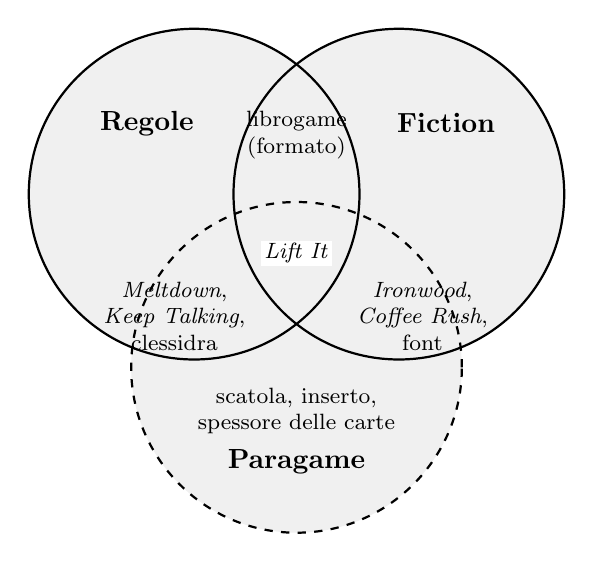
\begin{tikzpicture}[font=\small]
  \fill[gray!12] (0,0) circle (2.1cm);
  \fill[gray!12] (2.6,0) circle (2.1cm);
  \fill[gray!12] (1.3,-2.2) circle (2.1cm);
  \draw[thick] (0,0) circle (2.1cm);
  \draw[thick] (2.6,0) circle (2.1cm);
  \draw[thick, dashed] (1.3,-2.2) circle (2.1cm);
  \node[font=\bfseries] at (-0.6,0.9) {Regole};
  \node[font=\bfseries] at (3.2,0.9) {Fiction};
  \node[font=\bfseries] at (1.3,-3.4) {Paragame};
  \node[font=\footnotesize, align=center] at (1.3,0.75) {librogame\\(formato)};
  \node[font=\footnotesize, align=center] at (-0.25,-1.55)
    {\emph{Meltdown},\\\emph{Keep Talking},\\clessidra};
  \node[font=\footnotesize, align=center] at (2.9,-1.55)
    {\emph{Ironwood},\\\emph{Coffee Rush},\\font};
  \node[font=\footnotesize, align=center, fill=white, inner sep=1pt]
    at (1.3,-0.75) {\emph{Lift It}};
  \node[font=\footnotesize, align=center] at (1.3,-2.75)
    {scatola, inserto,\\spessore delle carte};
\end{tikzpicture}
\caption{Regole, fiction e paragame come tre aree con i bordi sfumati. Il paragame è
ciò che non è né regole né fiction, ma si sovrappone spesso a entrambe. La posizione
degli esempi riprende i commenti di Ruggero durante la lezione: \emph{Lift It} ``è al
centro'', \emph{Ironwood} aiuta soprattutto la fiction, \emph{Meltdown} e \emph{Keep
Talking and Nobody Explodes} soprattutto le meccaniche.}
\label{a10:fig:aree}
\end{figure}

\paragraph{Approfondimento: Genette e le ``soglie'' del testo.} Il termine
\emph{paratesto} viene dal critico francese Gérard Genette, che lo ha sistematizzato in
\emph{Soglie} (\emph{Seuils}, 1987). Per Genette il paratesto è ciò che fa di un testo
un libro e lo presenta al lettore: il titolo, il nome dell'autore, la copertina, le
dediche, le prefazioni, le note, ma anche il formato, la collana, la tipografia. È una
``soglia'' tra l'interno e l'esterno del testo, una zona di transizione che orienta la
lettura. L'idea di applicare lo stesso concetto ai giochi (paragame, paragioco) è
diffusa nei \emph{game studies}, dove il termine \emph{paratext} viene usato anche per
tutto ciò che circonda un gioco (\emph{trailer}, recensioni, guide, comunità). Nella
lezione di Ruggero il senso è più vicino a quello originale di Genette: le
caratteristiche materiali e formali dell'oggetto-gioco.

% ---------------------------------------------------------------------
\section{Le aree del paragame}
\label{a10:sec:aree}

``Su quali aspetti del paragame possiamo lavorare? E qui abbiamo l'ondata di robe.
Andiamo con calma: sono tante zone, ma sono sicuro che le vediamo tutte.'' La
tabella~\ref{a10:tab:aree} le riassume; le sezioni seguenti le vedono una per una.

\begin{table}[htbp]
\centering
\small
\begin{tabular}{@{}p{3.1cm}p{5.4cm}p{4.7cm}@{}}
\toprule
\textbf{Area} & \textbf{Domande da farsi} & \textbf{Esempi della lezione} \\
\midrule
Materialità & di che cosa sono fatti i componenti? Serve un'app? Quanto sono spesse
le carte? Clessidra o timer? & dadi di legno e di plastica; \emph{Lands of Galzyr} su
tablet e telefono; carte \emph{blue core}; \emph{standee} \\
Formato & come sono comunicati regole e testi? Che font, che dimensione, che misura
della carta? & \emph{Bureaucracy} di \emph{Magic}; il \emph{200 Word RPG} \\
Regolamento & quante pagine? Quanti libretti? Video, glossario, \emph{playthrough},
\emph{play aid}? & \emph{Irish Gauge}; \emph{Root}; riassunto delle icone \\
Scatola & dove andrà, nei negozi e a casa? & le vecchie scatole lunghe; la Kallax;
\emph{Dobro} \\
Grafica e illustrazioni & che cosa comunica l'aspetto visivo? Quante icone? &
\emph{Master of Rules}; \emph{Rolling Stock Stars}; \emph{A Feast for Odin} \\
Interfaccia analogica & com'è il \emph{wireframe}? Dove stanno le informazioni quando
il componente è in uso? & la carta di \emph{Magic}; la plancia di \emph{The
Gallerist}; le carte a ventaglio e i mancini \\
Ambiente & dove si gioca? Quanto spazio serve? Che suoni, che vibrazioni? & il tavolo
IKEA; il treno e l'aereo; \emph{Jenga} \\
Audio & serve una colonna sonora? & \emph{Escape: The Curse of the Temple} \\
Contesto & che cosa deve sapere chi gioca sul luogo e sulla cultura del gioco? &
\emph{Jakarta Traffic}; \emph{This War of Mine} \\
Lingua & il gioco dipende dalla lingua? & i giochi di Lacerda; \emph{Race for the
Galaxy}; \emph{Magic} \\
Spazio urbano e ibridi & la città, la stanza, il telefono come parte del gioco &
\emph{Pac-Manhattan}; \emph{Vroom}; \emph{World of Yoho} \\
\bottomrule
\end{tabular}
\caption{Le aree progettabili del paragame presentate a lezione, con le domande che
suggeriscono e gli esempi usati da Ruggero. Inserti e \emph{setup}, discussi alla fine
(sezione~\ref{a10:sec:inserti}), sono un'altra area della stessa famiglia.}
\label{a10:tab:aree}
\end{table}

% ---------------------------------------------------------------------
\section{Materialità}
\label{a10:sec:materialita}

La prima area è la \textbf{materialità}: ``le proprietà fisiche degli elementi di
gioco''. Legno, plastica, metallo. Prendiamo dei dadi classici di legno e dei dadi di
plastica: che cosa cambia? ``Il rimbalzo, il rumore, la sensazione al tatto.'' Sono
aspetti \textbf{cinestetici}, ``che assolutamente impattano''. Ma cambia anche altro,
``perché nel paragame spesso ci sono anche degli \textbf{aspetti culturali}''. In un
Eurogame, in un \emph{German}, si troveranno dadi di legno; in un \emph{American}, in un
\emph{dungeon crawler}, dadi di plastica. (Se n'era parlato, ``vagamente'', nella
lezione sui casi studio, a proposito dei componenti.)

\subsection{Il digitale come materiale}

Anche il \textbf{digitale} fa parte della materialità: se il gioco ha o richiede
un'app, un cellulare, un tablet, ``quello è un aspetto di materialità da considerare''.
Ruggero porta un esempio di un gioco che ha giocato, che la trascrizione chiama ``Lens
of Galsy''\footnote{Con ogni probabilità \emph{Lands of Galzyr} (Snowbright Studio,
2021), gioco d'avventura narrativo con app.}: ``molto carino, ma chiaramente pensato per
un tablet''. L'app ha tanto testo e tante cose a schermo, e sul cellulare, molto più
piccolo, ``non si vede niente''. ``L'app è la stessa, ma in base a dove lo stiamo
giocando, quel gioco può diventare un incubo di accessibilità, o qualcosa invece molto
più comodo da giocare.''

\subsection{Le carte non sono tutte uguali}

Quanto sono spesse le carte? Di che materiale sono? \emph{Blue core}, \emph{black
core}, \emph{white core}? ``Le carte non sono tutte uguali. Vi sembrano uguali perché le
usate da chi gioca, ma da produrre sono diverse.'' Quelle ``che si spaccano al volo'' si
riconoscono subito, perché sono le più economiche: di solito quelle di giochi come
\emph{Uno} o di giochi di carte ``più cheap da produrre'', in cui basta una pieghetta
per rovinare una carta ``forever and ever''. Altri giochi usano il \emph{blue core} o il
\emph{black core}; le carte di \emph{Magic}, per esempio, hanno il \emph{blue core}.

Ruggero semplifica la struttura: di solito una carta da gioco ha \textbf{tre strati},
lo strato con l'immagine sul fronte, quello con l'immagine sul retro, e in mezzo il
materiale che ne determina, tendenzialmente, la \textbf{rigidità}. ``Poi è più
complessa di così'', perché ci possono essere filigrane, texture e altro; ma la parte
centrale dice che cosa succede quando la carta si piega, o quando la si mescola male.

\paragraph{Le carte americane.} Una studentessa chiede delle carte da gioco americane,
``quelle di tela'', come le \emph{Bicycle}, che in Europa si vedono poco: c'è un motivo
per cui sono ``molto più fighe''? Sì: hanno una produzione che include \textbf{materiali
plastici} nella loro texture, che le rende più resistenti e crea un \textbf{attrito}
diverso. Sono carte che ``scivolano molto bene'' (``non ho più italiano, scusatemi''), e
infatti sono usatissime negli spettacoli di prestigiazione, perché si possono manovrare
velocemente, ``per chi le sa maneggiare; io no, di sicuro''. Le carte prodotte in Europa,
invece, hanno di solito un attrito molto più alto, e sono ``non fantastiche'' da usare
in modo ``sgaggio''.

\paragraph{Europa, America, Cina.} Lo stesso vale per i dadi: l'America fa un uso
abbondante di plastica nei giochi perché spesso produce in \textbf{Cina}, mentre
tipografie, stamperie e aziende che producono carte in Europa hanno ``molto poco
accesso'' a quei materiali. ``Quindi spesso siamo più forti nel legno e nella carta che
nella plastica.'' È ``un vaso di Pandora che a voi interessa il giusto'': per i progetti
del corso, quel tipo di finiture ``ve lo sognate, salvo pagare un bordello''. Ci sono
alcune fabbriche che possono fare cose bizzarre, nell'Est Europa e in Repubblica Ceca,
ma la maggior parte di chi produce stampa in Cina, oppure non usa quei materiali.

\paragraph{Miniature e \emph{standee}.} Stesso discorso per le miniature o gli
\textbf{\emph{standee}}, il cartoncino infilato in un piedistallo al posto della
miniatura di plastica. In un \emph{American} è facile trovare la plastica; in un gioco
prodotto e stampato in Europa, ``non trovate delle miniature di plastica'', perché non
c'è praticamente nessuna azienda europea di giochi da tavolo che possa stampare in
Europa la plastica a iniezione usata per le miniature; anche chi produce in Europa giochi
con parti di plastica le fa stampare in Cina. Per questo molti giochi europei degli anni
'90 e 2000, \emph{German} ed Eurogame, ``la plastica proprio la skippano'': se hanno
delle figure, sono \emph{standee}.

\paragraph{Approfondimento: che cosa fa davvero il ``core''.} Nella produzione di carte
da gioco lo strato centrale (\emph{core}) ha due funzioni: dà rigidità e soprattutto
rende la carta \textbf{opaca}, impedendo di vedere il fronte in controluce, cosa
essenziale in qualunque gioco con informazioni nascoste. \emph{Blue core} e
\emph{black core} sono nomi commerciali di cartoncini a più strati con un'anima
colorata scura. Sulle carte americane del tipo \emph{Bicycle}, il cartoncino è in
genere rivestito da una finitura goffrata e laccata (la cosiddetta \emph{air-cushion
finish}) che riduce l'attrito; le carte \emph{interamente} di plastica (PVC o acetato)
esistono, ma sono un prodotto diverso e più costoso.

\subsection{Clessidra o timer?}

``Occhio alla materialità, perché la materialità non va a impattare solo il paragame e
basta.'' Il classico esempio di materialità che impatta anche le \textbf{regole} è la
\textbf{clessidra}. Che differenza c'è tra un timer sul cellulare e una clessidra? Uno
studente risponde: ``la tangibilità''. Sì, e soprattutto quella che si chiama di solito
l'\textbf{informazione discreta}: con il timer si sa con precisione quando mancano un
secondo, due, tre, quattro secondi. Con la clessidra no: si vede chiaramente quando è
finita, ma ha ``quel pizzichino di incertezza che crea una tensione molto precisa che il
timer non ha''. Entrambi creano tensione, adrenalina, frenesia, ma in modo diverso; e
sapere quale dei due serve al proprio gioco ``non è così scontato''
(tabella~\ref{a10:tab:clessidra}).

\begin{table}[htbp]
\centering
\small
\begin{tabular}{@{}p{3cm}p{5cm}p{5cm}@{}}
\toprule
 & \textbf{Timer (cellulare)} & \textbf{Clessidra} \\
\midrule
Informazione & discreta e precisa: si sa quanti secondi mancano & continua e
incerta: si vede la sabbia scendere, ma non si sa con precisione quanto manca \\
Tensione & c'è, ed è ``contata'' & c'è, con ``un pizzichino di incertezza'' in più \\
Fiction & neutra, a meno di suoni scelti apposta & può essere diegetica (vedi il
fiammifero di \emph{Scandal in the Deep}, sezione~\ref{a10:sec:casi}) \\
Domanda da farsi & perché un timer e non una clessidra? & perché una clessidra e non
un timer? \\
\bottomrule
\end{tabular}
\caption{Timer e clessidra come scelta di materialità che incide sulle regole e sulla
tensione di gioco.}
\label{a10:tab:clessidra}
\end{table}

Qui Ruggero fa un annuncio che vale per il resto del corso: ``io ve lo ricordo, ve
l'avevo già accennato, ve lo ripeto: quando vedremo i \emph{pitch}, ma anche i vostri
progetti più avanti, nelle ultime lezioni, \textbf{io vi chiederò tantissimi
perché}''. Perché avete scelto una cosa, perché l'avete fatta, perché l'avete decisa.
``Se avete una clessidra e non un timer, io vi chiederò perché avete una clessidra e non
un timer. Perché avete la plastica, la carta, e così via. Voi dovete dirmi il perché
delle cose che fate.''

% ---------------------------------------------------------------------
\section{Formato}
\label{a10:sec:formato}

Il \textbf{formato} è il modo in cui sono comunicati, per esempio, regole e testi:
frasi o icone? Che font? Quanto è alto, che dimensione ha? E la carta, com'è fatta,
quanto è grande?

\paragraph{\emph{Bureaucracy}.} Il primo esempio è una carta di \emph{Magic} ``volutamente
fatta male'': \emph{Bureaucracy}, da una di quelle serie \emph{easter egg} (umoristiche)
che \emph{Magic} pubblica ogni tanto\footnote{La trascrizione aggiunge un dettaglio
sul simbolo dell'espansione che non è ricostruibile (``ha l'uomo rotto suonate come
simbolo''). \emph{Bureaucracy} appartiene alle espansioni parodiche di \emph{Magic}, le
cosiddette \emph{Un-set}.}. Per il testo è stato scelto un font piccolissimo (``mi
sembra che fosse un corpo 5, o addirittura 6''), per renderlo ``un muro di testo
oppressivo'': tematicamente coerente con il nome della carta.

\paragraph{La misura delle carte di \emph{Magic}.} Qualcuno sa quanto sono grandi le
carte di \emph{Magic}? ``Una dimensione da poker.'' In millimetri sono ``cifre
bizzarre'', perché in realtà la misura è di \textbf{3,5 per 2,5 pollici}\footnote{La
trascrizione riporta cifre storpiate (``88,4 per 69,5''). 3,5 per 2,5 pollici sono circa
88,9 per 63,5 millimetri; la misura nominale indicata di solito per le carte di
\emph{Magic} è 63 per 88 millimetri.}, ``in un sistema stupido americano di
misurazione'' (``ormai l'ho detto, è troppo tardi''). E in quella dimensione non c'è
tutto lo spazio che si vuole, perché una parte è dedicata all'\textbf{illustrazione}:
lo spazio per il testo, con il font e la dimensione scelti, è ancora più ridotto.
Questo non impatta solo il formato, ma anche le \textbf{regole}: ``una regola complessa
sarà difficile da scrivere in quello spazio'', e quindi il formato costringe a scegliere
regole che ci stiano dentro.

\paragraph{Il \emph{200 Word RPG}.} Un caso estremo: il \emph{200 Word RPG}, una sfida
in cui si scrivono giochi di ruolo completi in \textbf{200 parole}. Il paragame è il
formato stesso delle 200 parole: ``ditemi voi se non vi impatta le regole, quel
formato''.

``Non prendete questa cosa qua come del contorno, come una cosa che è un di più.
Questa roba qui vi va a impattare come voi create i giochi, e se lo sapete, potete
lavorarci attorno.''

% ---------------------------------------------------------------------
\section{Regolamento}
\label{a10:sec:regolamento}

Il \textbf{regolamento} è un'area a sé. Quante pagine ha? Una o quaranta? Che cosa
cambia? ``Se io vi dico: venite, c'è un party game, e tiro fuori un manuale da 60
pagine, che cosa succede?'' Succede che nessuno lo gioca.

\paragraph{\emph{Irish Gauge}: un caso positivo.} All'opposto, un caso ``incredibile'':
\emph{Irish Gauge}\footnote{La trascrizione dice ``Irish Gouge'' e attribuisce il gioco a
``Amable Holland'', più avanti ``Anne Blowland''. È \emph{Irish Gauge}, gioco
ferroviario di Amabel Holland.}, un gioco economico ferroviario ``bellissimo'', di circa
un'ora di partita, in cui si comprano azioni e si costruiscono ferrovie, con una
complessità significativa sul tavolo, ``un gioco comunque bello intenso''. E il
regolamento è \textbf{un singolo foglio di carta} ``che lascia zero dubbi dopo che lo si
è letto''. ``Bellissimo, irraggiungibile forse.'' È una sorpresa positiva; il caso
contrario (il party game da 60 pagine) è una sorpresa negativa che uccide il gioco.

\paragraph{QR code e video.} Chi gioca spesso avrà notato che sempre più regolamenti
hanno un \textbf{QR code} o un link a un video in cui le regole vengono spiegate.
Perché? ``Non sappiamo più leggere'' è ``la versione più nichilista''. La risposta ``più
banale e meno nichilista'' è che \textbf{le persone imparano in modi diversi}: un
regolamento scritto in un certo modo può andare benone per una persona ed essere un
disastro per un'altra.

\paragraph{Più libretti per lo stesso gioco.} Alcuni giochi hanno più di un libretto di
regole. \emph{Root}, per esempio, ha la \textbf{guida rapida} (il \emph{learn to play}),
scritta come un regolamento da leggere al tavolo, e la \textbf{Legge di Root}, scritta
come un \textbf{manuale tecnico}: paragrafi 1.1.1, 1.1.2, 1.1.3, 1.2.1 e così via, con
glossario. ``Il gioco è lo stesso. Lo si impara a giocare in entrambi i modi, ma parlano
a due persone completamente diverse.''

\paragraph{I costi.} Ogni scelta ha un costo. Un regolamento in più costa la
produzione di un regolamento in più, \textbf{a ogni copia} stampata. Il video è un costo
diverso: lo si paga una volta, all'inizio, lo si mette online ``e quel video lì è lì''.
``Se tu stampi 100 copie o ne stampi 10.000, il video non ti costa di più. Il
regolamento sì.''

\paragraph{Glossario, \emph{playthrough}, \emph{play aid}.} Altre domande: c'è un
\textbf{glossario}? Un \emph{playthrough}? Un \emph{play aid}? E le icone, dove sono
riassunte? Dove si trova di solito il riassunto delle icone? Due risposte, ``entrambe
vere''. Tancredi: \textbf{nell'ultima pagina del regolamento}, usata spesso proprio per
questo, perché si può tenere il regolamento girato sul tavolo e avere il riassunto
davanti. Tiziana: in un \textbf{\emph{play aid}}, un cartoncino, magari uno a persona,
con il riassunto delle icone. Quando l'uno e quando l'altro? Dipende da \textbf{quante
icone} ha il gioco. In \emph{Race for the Galaxy} un riassunto a testa non esiste,
``perché il riassunto delle icone di \emph{Race for the Galaxy} è così'' (e Ruggero
mostra quanto è lungo). In giochi con cinque, sei, una decina di icone è facile avere
una carta personale che le riassume, magari con il \textbf{flusso del turno} sul retro.

\paragraph{Il \emph{playthrough} e l'\emph{actual play}.} Più avanti, su richiesta di
uno studente (``Ruggero, non so se l'hai detto: il \emph{playthrough}?''), Ruggero torna
sul punto. Il \textbf{\emph{playthrough}} è \textbf{una giocata descritta}. Molti giochi
lo fanno spezzandolo in esempi: i classici esempi in cui ``Tizio e Caio fanno A, B, C,
poi Tizio fa B e Caio piange perché ha perso la partita''. Questi esempi non sono solo
un'applicazione delle regole: sono una descrizione di \textbf{che cosa fanno le persone
al tavolo}. Alcuni giochi, soprattutto di ruolo, includono il cosiddetto \textbf{\emph{actual
play}}: un'intera partita descritta, alternando le parti di \emph{roleplay} e quelle
meccaniche (``Tizio tira e fa 18, quindi apre questa cosa; poi Caio dice questa cosa con
il suo personaggio''). Dove si trovano\footnote{La trascrizione attribuisce la domanda a
qualcuno che si rivolge a ``Pietro''; con ogni probabilità è un errore di trascrizione
per ``Ruggero''.}? Sono ``comunissimi nei giochi di ruolo'': molti giochi di ruolo
contemporanei hanno esempi di \emph{actual play}, di solito in fondo al manuale. Gli
esempi sparsi nei regolamenti sono ``un'estrazione del \emph{playthrough}'', scritti con
la stessa idea; il \emph{playthrough} vero e proprio è l'esempio di partita completa. Nei
giochi da tavolo più commerciali è raro, ``perché le pagine dei regolamenti costano'', e
una partita completa prende molto spazio. Rientra quindi soprattutto nei giochi di
ruolo, che hanno già manuali da cento pagine e passa e non hanno il problema di stare
sotto le 16 pagine, ``perché sennò la gente si spaventa'' davanti a un regolamento da
20.

% ---------------------------------------------------------------------
\section{La scatola}
\label{a10:sec:scatola}

Nel formato rientra anche la \textbf{scatola}. Ruggero è convinto di averne già parlato
(``non abbiamo mai parlato delle scatole? Secondo me no'') e la affronta con una
domanda: come erano fatte le scatole del vecchio \emph{Risiko!} o del vecchio
\emph{Monopoly}? ``Basse e lunghe.'' Perché? ``Ci stava il tabellone''; ``si impilavano''.
La domanda, precisa Ruggero, non è che cosa c'era dentro, ma \textbf{dove doveva andare}
la scatola: nei negozi di giocattoli e, a casa, dove venivano messi i giochi trenta,
quarant'anni fa? Non nella libreria: \textbf{negli armadi}. ``Non era una questione
estetica'': l'armadio è stretto e lungo, e la scatola doveva entrare lì.

E oggi, dove vanno messi? In libreria. Quale libreria? La \textbf{Kallax}\footnote{La
trascrizione dice ``Callax'' e, a tratti, ``Galaxy''.} dell'IKEA, ``la libreria più
venduta del mondo''. Com'è fatta? ``\textbf{A cubi}.'' La scatola del vecchio
\emph{Monopoly} lì dentro non entra (``puoi metterla in cima, certo''). Ma se oggi un
editore vuole che il suo gioco entri ``nella libreria più venduta del mondo'', il gioco
deve entrare in un cubo. ``È tutto qui. \textbf{Una scelta dell'IKEA ha deciso che le
nostre scatole ora sono quadrate}.'' L'IKEA non ha convinto gli editori di niente: ``è
una roba che viene naturale, perché tutta l'umanità è intrecciata. Le decisioni che
prende qualcuno vanno a impattare qualcun altro''. Chi vuole che il proprio gioco sia in
vista in libreria deve fare i conti con il cubo.

Ruggero si concede qui una raccomandazione generale: ``se c'è una cosa che voglio che vi
portiate via da questo corso, una cosa'' (``poi, se fate anche giochi dopo, belli,
benissimo''), ``la cosa migliore per me, perché sono contento, ho fatto il mio lavoro,
posso morire in pace'', è questa: \textbf{ragionate quando fate le cose}. ``Potete
ragionare sulle cose quanto volete. Più ci ragionate, più avete aree operative su cui
fare le cose.''

\paragraph{Approfondimento: il ``formato Kallax''.} Il vano interno di una Kallax misura
circa 33 per 33 centimetri, per una profondità di poco inferiore ai 39. Non a caso un
gran numero di giochi da tavolo contemporanei di formato ``standard'' ha una scatola
quadrata di circa 30 centimetri di lato: è il formato che sta in un vano in piedi o
coricato, e che si impila bene. Molti editori lo indicano ormai esplicitamente tra i
vincoli di progettazione della scatola, insieme al peso e ai costi di spedizione.

% ---------------------------------------------------------------------
\section{Grafica e illustrazioni}
\label{a10:sec:grafica}

``\textbf{Graphic design e illustrazioni sono due cose diverse}. Non confondete le
cose.'' Le \textbf{illustrazioni} sono tendenzialmente l'\emph{art}: le immagini,
gli sfondi, i personaggi, i luoghi, la parte di \emph{world building}. Il
\textbf{graphic design} sono le icone, la UX. ``Non fate fare queste due cose alla
stessa persona, sennò di solito viene una porcheria.''

\subsection{Due edizioni, due destini}

Sulla slide ci sono due scatole: una con un omino che tiene sopra di sé delle forme, e
una con un'auto sotto un cielo stellato, una notte al neon. ``Sono lo stesso gioco'':
\emph{Master of Rules}\footnote{Il titolo è quello della trascrizione e non è stato
possibile verificarlo.}, ``un gioco bellissimo'', che nella sua edizione americana è
uscito con la prima scatola. ``Vi sorprenderà sapere che in America non è andato per
niente, nonostante sia un gioco incredibile. Qualcuno ha un'idea del perché?'' Le
risposte sono impietose: ``fa schifo'', ``sembra quelli che trovi in edicola''. E
dentro, dice Ruggero, ``è ancora più brutto''.

Uno studente lo provoca: ``io ho dei giochi che hanno copertine orrende da 100 euro'':
gli \textbf{Splotter}\footnote{Splotter Spellen, editore olandese noto per giochi
molto pesanti e per una grafica spartana.}. Ruggero non lo nega, ma ribalta la
domanda: la grafica degli Splotter ``è comprensibile perché la fanno così, ovvero perché
non gliene frega niente''; ma ``sarebbero giochi peggiori con una grafica migliore?'' ``La
risposta, nel tuo cuore, la sai: no.'' Le immagini danno un'esperienza, un \emph{look
and feel}.

Tiziana porta un caso concreto: un amico ha comprato \emph{Darwin's Journey}\footnote{
La trascrizione dice ``Darvis Journey''.}, ``un gioco che secondo me è bellissimo'', e
l'ha rivenduto, perché l'impatto grafico per lui è stato terribile: ``colori scuri sul
marrone''. ``Non riusciva a vederlo.''

Ruggero avrebbe potuto fare ``mille altri esempi'' di giochi usciti in due edizioni con
grafiche diverse, ``una che va a picco e non la vedete più, e l'altra che invece diventa
roba di culto''. Perché la grafica ha un impatto ``non solamente in termini di
leggibilità, ma anche di \emph{vibes}''. Lui, personalmente, non ci fa caso: ``io mi
gioco anche \emph{Rolling Stock Stars}'', che ``sembra fatto da marito e moglie su
Excel''. Ma altre persone vedono quella grafica e dicono ``non giochiamo a \emph{Rolling
Stock Stars}''. E finisce che ``il piccolo Ruggero'' lo gioca ``una volta ogni cinque
anni, perché nessuno vuole giocarci''. La conclusione: ``un gioco può beneficiare
dall'essere \textbf{non visivamente ostile} alle persone che lo vogliono giocare''.
Un altro studente aggiunge, a proposito di grafiche difficili, \emph{Terraforming
Mars} (``la carta con il cane''), e Ruggero si arrende: ``volete farmi stare male
oggi''.

\subsection{Il font, e quante icone}

Anche il \textbf{font} rientra nella grafica, non solo nel formato: il font del titolo,
il font dei contenuti. Ruggero cita un gioco che ha venduto ``proprio per il font che
aveva'', e promette di mostrarlo dopo, perché ``ci vuole del tempo per elaborare''
(lo farà nella discussione finale: è \emph{Al Rashid}, sezione~\ref{a10:sec:alrashid}).

Ultimo punto della grafica: \textbf{quante e quali icone} avete? Sulla slide c'è \emph{A
Feast for Odin}\footnote{La trascrizione dice ``Fist for Odin''. \emph{A Feast for
Odin} (Uwe Rosenberg, 2016).}: ``quel gioco lì ha 50 azioni diverse. Non devo dirvi
altro''. Ragionate sulle icone che avete.

\paragraph{L'intervento di Tiziana.} Tiziana porta un esempio di segno opposto: ha
giocato di recente a un gioco che la trascrizione chiama ``MNFR''\footnote{Il titolo
non è ricostruibile dalla trascrizione.}, abbastanza complesso, con varie tipologie di
azioni e una serie di cose che si succedono; ma le icone ``sono sempre quelle'', in
numero limitato, e una volta capite ``te le ritrovi in tutte le salse, nelle varie parti
e sezioni del gioco''. ``E questo aiuta molto.'' Ruggero concorda e cita di nuovo
\emph{The Gallerist} (``bellissimo, un capolavoro''): sono giochi in cui, se si fa un
buon lavoro sulle icone, il gioco ``non ti chiederà mai di andare a leggere il
regolamento durante la partita''. Lui ha giocato di recente un Eurogame di designer
giapponesi\footnote{La trascrizione dice ``Elder Tide degli stessi di Gisoji''; titolo
e autori non sono ricostruibili con sicurezza.}, con un \emph{setting} un po' fantasy, in
cui si costruiscono edifici su un'isola e ci si muove di porto in porto per vendere
risorse: ``ha tante icone, ma dopo i primi cinque minuti, per tutte le altre due ore
della partita, non abbiamo guardato il regolamento una singola volta, perché è tutto
chiaro, tutto immediato''. Si torna ai pilastri: immediatezza, efficienza,
memorabilità.

% ---------------------------------------------------------------------
\section{Interfaccia analogica}
\label{a10:sec:interfaccia}

La voce successiva è l'\textbf{interfaccia analogica}: ``si parla di
\emph{wireframing}, di solito''. È la struttura nuda della carta, quelle linee che, in
stampa, ``verranno abbellite da frame, cornici''. Ma il \emph{wireframe} è quello. ``Se
vi chiedo di disegnarmi a occhi chiusi su un foglio una carta di \emph{Magic}, voi sapete
come disegnarmela'': divisa a metà, al centro un rettangolino molto sottile, un
rettangolo più grosso in alto, uno più grosso in basso. ``Quella parte lì è una parte su
cui potete ragionare.''

\subsection{La scatola in piedi: \emph{Dobro}}

Anche la grafica della scatola è interfaccia. ``Se io prendo la scatola e la metto in
verticale, posso leggere il titolo?'' C'è una ``diatriba'' che Ruggero non apre
(``siete ancora persone sane di mente, non voglio rovinarvi la vita''): i giochi da
tavolo si mettono in libreria in verticale o in orizzontale? Lui fa un mix, ma molte
persone li mettono in verticale, e molte scatole non hanno il nome del gioco su tutti i
lati: alcune lo hanno solo per il lungo, e in verticale il nome è storto. L'esempio
positivo è \emph{Dobro}, di cui il suo gruppo ha rifatto la scatola per l'edizione
italiana: un lato lungo con il nome in orizzontale, il lato opposto con il nome in
verticale, e lo stesso sui due lati corti. ``Non importa come la mettete: un modo per
trovarla con il nome che si vede da fuori lo trovate sicuramente.'' Mentre ``ho delle
scatole in cui non si vede il nome, perché purtroppo non l'hanno messo su tutti i
lati''. Quindi: \textbf{la grafica della scatola non va lasciata al caso}, ``perché è
funzionale''. (``Mi sto arrabbiando, si vede, perché questa cosa mi fomenta.
Purtroppo per voi.'')

\subsection{Le opere sulla plancia di \emph{The Gallerist}}

Una studentessa chiede di chiarire: l'interfaccia analogica è il discorso della scatola
e della visibilità, o altro? Ruggero torna al \emph{wireframe}, ``cioè a come sono fatte
le carte'', e porta l'esempio di \emph{The Gallerist}: si acquistano opere d'arte da
esporre nella propria galleria, e la \textbf{plancia} personale raffigura la galleria.
Le tre tessere delle opere esposte si sovrappongono perfettamente ai \textbf{muri
disegnati sulla plancia}, ``andando letteralmente a mettere le opere in vista nella
nostra galleria''. Non è casuale: hanno pensato la grafica in modo che aiutasse a capire
che cos'è quel componente, e in modo che fosse anche soddisfacente. Di nuovo:
soddisfazione, efficienza, memorabilità, immediatezza.

\subsection{Dove stanno le informazioni quando le carte sono in mano}

Un altro aspetto dell'interfaccia è \textbf{dove si piazzano le informazioni}. Con le
carte da poker in mano, dove sono le icone? \textbf{In alto a sinistra}: quando le carte
sono aperte a ventaglio, ciascuna copre buona parte di quella precedente, e l'angolo in
alto a sinistra è ``la cosa più visibile'' (figura~\ref{a10:fig:ventaglio}).

Tancredi apre una parentesi sui \textbf{mancini}: ``io da mancino, tutte le volte che
apro le carte da poker, non vedo assolutamente niente''. Ruggero conferma (``ho degli
amici mancini, e se avete un gioco che non pensa ai mancini lo sapete al volo, perché
ve lo dicono''), e lo riconduce all'\textbf{accessibilità}: i mancini tengono in mano le
carte come tutti, ``è solo che per natura il ventaglio lo fanno nell'altro verso''. Molti
giochi per questo \textbf{duplicano} il seme della carta, mettendolo anche in alto a
destra. In alcuni giochi è più complicato: quando l'angolo in alto a sinistra ospita
icone meccaniche, come il costo, come in \emph{Race for the Galaxy} (``è il problema
minore di questa carta, mi sento di dire''), duplicare vuol dire affollare ancora di più
una carta già piena. ``Volete davvero duplicare le informazioni di questa carta
dall'altro lato? Io non lo farei.'' Non sempre si può; ma ``è assolutamente una
considerazione da fare''.

\begin{figure}[htbp]
\centering
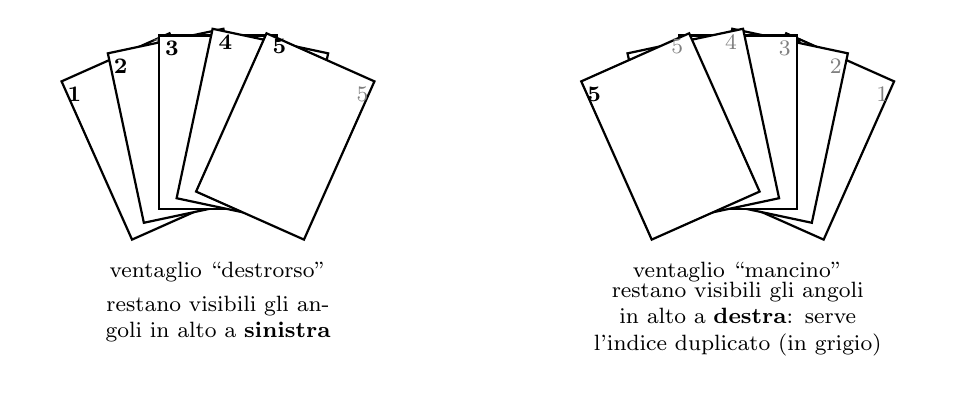
\begin{tikzpicture}[font=\footnotesize]
  % mano destrorsa: ventaglio verso destra
  \begin{scope}[shift={(0,0)}]
    \foreach \a/\i in {24/1, 12/2, 0/3, -12/4, -24/5}{
      \begin{scope}[rotate around={\a:(0,-2.6)}]
        \draw[thick, fill=white] (-0.75,-1.6) rectangle (0.75,0.6);
        \node[anchor=north west, inner sep=2pt] at (-0.75,0.6) {\textbf{\i}};
        \node[anchor=north east, inner sep=2pt, text=gray] at (0.75,0.6) {\i};
      \end{scope}
    }
    \node at (0,-2.4) {ventaglio ``destrorso''};
    \node[text width=4.6cm, align=center] at (0,-3.0)
      {restano visibili gli angoli in alto a \textbf{sinistra}};
  \end{scope}
  % mano mancina: ventaglio nell'altro verso
  \begin{scope}[shift={(6.6,0)}]
    \foreach \a/\i in {-24/1, -12/2, 0/3, 12/4, 24/5}{
      \begin{scope}[rotate around={\a:(0,-2.6)}]
        \draw[thick, fill=white] (-0.75,-1.6) rectangle (0.75,0.6);
        \node[anchor=north west, inner sep=2pt] at (-0.75,0.6) {\textbf{\i}};
        \node[anchor=north east, inner sep=2pt, text=gray] at (0.75,0.6) {\i};
      \end{scope}
    }
    \node at (0,-2.4) {ventaglio ``mancino''};
    \node[text width=4.6cm, align=center] at (0,-3.0)
      {restano visibili gli angoli in alto a \textbf{destra}: serve l'indice
      duplicato (in grigio)};
  \end{scope}
\end{tikzpicture}
\caption{Le carte a ventaglio. L'informazione più importante va nell'angolo che resta
scoperto; chi apre il ventaglio nell'altro verso, come molti mancini, vede l'angolo
opposto, e per questo molti giochi duplicano il seme o l'indice in alto a destra.
Schema illustrativo: l'ordine con cui le carte si sovrappongono dipende da come le si
apre.}
\label{a10:fig:ventaglio}
\end{figure}

Ruggero annuncia che su grafica e formato c'è ``un'altra cosa'', da riprendere dopo (lo
farà con gli inserti, sezione~\ref{a10:sec:inserti}).

% ---------------------------------------------------------------------
\section{Ambiente}
\label{a10:sec:ambiente}

\textbf{Dove} giocheranno le persone al vostro gioco? Su un tavolo, a letto, per terra,
in piedi? E \textbf{quanto spazio} prende il gioco? Qualcuno sa quanto spazio, al
massimo, deve prendere un gioco da tavolo \emph{family} per quattro persone? ``La sapete
nel vostro cuore, la risposta.'' Gianmarco: ``\textbf{il tavolo IKEA}''. ``Bravissimo,
Gianmarco, è sempre quello.'' Il tavolo IKEA più venduto: cercate quanti centimetri
misura. ``Se il vostro gioco non entra in quel tavolo, avete un grosso problema.''

E se è un \textbf{party game}? Allora deve stare nel \textbf{tavolino da caffè}
dell'IKEA, più piccolo, quello da divano, ``per un altro tipo di ambiente''. Se è un
gioco \emph{pocket}, portatile, deve stare nei tavolini da caffè, in quelli del
\textbf{treno}, in quelli dell'\textbf{aereo}. ``Quanto spazio prende il vostro gioco
apparecchiato non è casuale. Non lasciate al caso quella roba'', altrimenti succede,
come è capitato di vedere a Ruggero, di avere ``giochi in solitaria che prendono un
tavolo per sei persone''.

Il mezzo di trasporto ha poi un altro problema: il treno e l'aereo \textbf{si muovono}.
Il gioco può starci come spazio, ma i componenti? Uno studente ricorda le
\textbf{versioni magnetiche} di scacchi e dama, e una versione mini di \emph{Azul} con
le tessere che si incastrano. E Ruggero aggiunge: \emph{Jenga} ci sta, come spazio, nel
tavolino di un aereo. Perché nessuno ci gioca in aereo? ``Per le vibrazioni dovute al
movimento.'' Appunto: ``l'ambiente non è solo spazio. L'ambiente è anche suoni, è anche
vibrazioni, è un sacco di altre cose''.

\paragraph{Approfondimento: misurare il tavolo.} Le misure dei tavoli più diffusi
nelle case cambiano da modello a modello, ma un tavolo da cucina per quattro persone ha
spesso un piano tra gli 80 per 80 e i 120 per 75 centimetri, e un tavolino da caffè è
molto più piccolo (spesso intorno ai 90 per 55 centimetri). Il consiglio di Ruggero va
preso alla lettera: misurare il piano reale di riferimento e fare un \emph{mock-up} del
gioco apparecchiato a grandezza naturale, lasciando spazio per le mani, i bicchieri, le
plance personali e i mazzi degli scarti. È uno dei test più economici che si possano
fare con un prototipo.

% ---------------------------------------------------------------------
\section{Audio}
\label{a10:sec:audio}

Altra area progettabile: l'\textbf{audio}. Serve la musica nel vostro gioco? Alcuni
giochi usano una \textbf{colonna sonora} per dare il tempo. L'esempio è \emph{Escape:
The Curse of the Temple}\footnote{La trascrizione inciampa più volte sul titolo, e
Ruggero stesso si corregge (``scusatemi, perché in tedesco\dots''). Il gioco è
\emph{Escape: The Curse of the Temple} (Kristian Amundsen \O{}stby, Queen Games, 2012).}: un
gioco in tempo reale in cui bisogna uscire dal tempio entro la durata della colonna
sonora, ``sennò siete fritti''. E a intervalli la colonna sonora fa sentire dei
\textbf{colpi di gong} che attivano eventi meccanici nel gioco. Quindi la colonna
sonora non è ``solamente un timer, una grossa clessidra'': è un \textbf{elemento
meccanico} che, con l'audio, fa altre cose. E fa anche \textbf{fiction}: dà elementi di
\emph{world building}, certe \emph{vibes}. ``È chiaro che \emph{Escape} è molto Indiana
Jones: non avete una colonna sonora techno IDM a palla.''

% ---------------------------------------------------------------------
\section{Contesto}
\label{a10:sec:contesto}

``Al \textbf{contesto} non ci pensa quasi mai nessuno, ma è molto importante'', perché
informa il gioco, ``non solo in termini di \emph{world building}, ma anche in termini di
che cosa vuole che voi facciate''.

\paragraph{\emph{Jakarta Traffic}.} \emph{Jakarta Traffic}\footnote{Titolo come nella
trascrizione.} è un gioco sul traffico di Giacarta, ``che è molto ostile'': si naviga il
traffico per fare delle consegne, e molti elementi del gioco sono \textbf{culturali}.
Spiegare le meccaniche a chi non sa come è fatta Giacarta, culturalmente, rende il gioco
molto più complesso di quanto dovrebbe essere. Qui, secondo Ruggero, hanno fatto un
buon lavoro: il manuale aiuta a capire il contesto, e hanno perfino creato una colonna
sonora usando il traffico di Giacarta come \emph{sample}, per creare un certo
\emph{mood}.

\paragraph{\emph{This War of Mine}.} Ma il contesto non è solo \emph{setting}: può
anche \textbf{informare le scelte}. Qualcuno conosce il gioco da tavolo di \emph{This War
of Mine}\footnote{La trascrizione dice ``Diceworld Mine''.}? Qual è il suo contesto?
``È una guerra, ma non mi ricordo se è una guerra vera.'' ``È a metà'': non è scritto
apertamente, ma è palesemente l'\textbf{assedio di Sarajevo}. E soprattutto, non si
giocano militari: si giocano \textbf{civili}. Se ci si approccia al gioco ``con tutto il
bagaglio culturale dei giochi di guerra'', ci si aspettano cose che il gioco non può
dare, perché ``non è un gioco di soldati in guerra: è un gioco in cui c'è la guerra, ma
non è un gioco di guerra''. Queste cose si risolvono con un mix: in parte con testo,
\emph{flavor} e \emph{world building}, in parte con il paragame, con i materiali.

% ---------------------------------------------------------------------
\section{Lingua}
\label{a10:sec:lingua}

Anche la \textbf{lingua} è un componente. Alcuni giochi sono \textbf{indipendenti dalla
lingua}: in un gioco di Lacerda\footnote{Vital Lacerda, autore portoghese di Eurogame
pesanti, tra cui \emph{The Gallerist}.}, o nella maggior parte dei \emph{German}, sulle
carte non c'è testo, ``alla buon'icona''. Lo stesso \emph{Race for the Galaxy}, lasciando
stare il nome e l'effetto ricopiato sotto, si può giocare anche senza leggere l'inglese:
``mi basta sapere che cosa fanno quelle icone''. Così \emph{The Gallerist}, o \emph{Master
of Rules}. Altri giochi no: \emph{Magic} è molto difficile da giocare se le carte non sono
nella propria lingua.

% ---------------------------------------------------------------------
\section{La città, la stanza, il telefono}
\label{a10:sec:pervasivo}

``In quali altri modi posso impattare l'esperienza di chi gioca senza passare per le
regole e per la fiction?'' Sulla slide c'è un'immagine di
\textbf{\emph{Pac-Manhattan}}\footnote{La trascrizione dice ``Pac-Man Hatton''.
\emph{Pac-Manhattan} (2004) è un gioco urbano nato alla New York University, in cui
persone vere interpretavano Pac-Man e i fantasmi nelle strade di Manhattan.}: la città,
gli aspetti \textbf{pervasivi urbani} sono anch'essi paragame.

\paragraph{La stanza come pista.} Un altro esempio è un gioco di corsa cooperativo che
la trascrizione chiama ``Vroom''\footnote{Il titolo non è stato possibile verificarlo.}:
usa il \textbf{tavolo} come spazio di gioco e chiede di prendere degli \textbf{oggetti
della propria stanza} e metterli sul tavolo come ostacoli, ``fisicamente, proprio''.

\paragraph{\emph{World of Yoho}.} Infine \emph{World of Yoho}\footnote{La trascrizione
dice ``World of Yacht'', ``World of YOHO'', ``Word of Yoko''.}, un gioco di pirati che
chiede di usare il \textbf{cellulare} su un tabellone gigantesco. Il telefono è la
propria \textbf{nave}: quando lo si sposta, sullo schermo si muove la mappa, e le parti
di quella casella di mare diventano interagibili in digitale. ``Si poteva fare senza
cellulare? Sì, con un libro degli eventi gigantesco, una seccatura infinita. Mentre così
è una cosa immediata, che si spiega in tre minuti.'' Uno studente chiede se si giochi su
un tabellone normale: sì, il gioco arriva in scatola con il suo tabellone, che si mette
sul tavolo, e chiede semplicemente di usare il telefono come nave per tutta la partita.
Ogni persona usa il proprio telefono; e nelle battaglie navali ``vedi i proiettili che
vengono sparati da una nave, che vanno sul bordo del telefono ed entrano nell'altro.
Pazzi completi. Bellissimo''.

\medskip
Prima dei casi studio, una seconda pausa: ``sono le 57'', e Ruggero dà otto minuti
``per il numero tondo'': si riprende alle 19:05.

% ---------------------------------------------------------------------
\section{Casi studio}
\label{a10:sec:casi}

``Andiamo avanti nell'ultima parte'': i \textbf{casi studio}, per vedere ``come
applichiamo le cose che abbiamo appena visto a giochi particolari''. Ce ne sarebbero
``a tonnellate''; Ruggero ne ha scelti un gruppo ``che va da giochi più regolari a cose
più \emph{deranged}, come spesso succede'', e per ciascuno dovrebbe essere chiaro perché
è stato scelto. La tabella~\ref{a10:tab:casi} li riassume.

\begin{table}[htbp]
\centering
\small
\begin{tabular}{@{}p{3.3cm}p{5.3cm}p{4.6cm}@{}}
\toprule
\textbf{Gioco} & \textbf{Elemento di paragame} & \textbf{Che cosa tocca} \\
\midrule
\emph{Cuba Libre} & due regolamenti, due diagrammi di flusso per i bot, quattro
brochure di fazione & regole, accessibilità di un gioco pesante \\
\emph{193 Days} & solo un mazzo di carte, niente regolamento & si impara giocando \\
gioco ``a metropolitana'' & creazione del personaggio piegata come una mappa turistica
& fiction, \emph{world building} \\
\emph{Shenzhen I/O} & un manuale fisico da stampare, il faldone della collector's &
meccaniche (le schede tecniche), fiction, ``feeling'' \\
pinball in scatola & dadi da schicchera su una ``scalinata'' con i flipper & meccaniche \\
\emph{Lift It} & la gru da mettersi in testa & ``al centro'' di regole, fiction e
paragame \\
\emph{Coffee Rush} & tazzine di plastica e ingredienti a forma di ingrediente & fiction,
\emph{vibes} \\
\emph{Ironwood} & una fazione tutta di legno, una tutta di metallo & fiction,
riconoscibilità, \emph{vibes} delle fazioni \\
\emph{Nyctophobia} & occhiali oscuranti per chi scappa & meccaniche, accessibilità,
fiction \\
\emph{Keep Talking and Nobody Explodes} & visore VR da una parte, manuale di carta
dall'altra & meccaniche, comunicazione \\
\emph{City of Six Moons} & nessun regolamento: un artefatto ``alieno'' & il gioco stesso
è dedurre le regole \\
\emph{Scandal in the Deep} & un fiammifero acceso come torcia & tempo reale, fiction
diegetica \\
\emph{Metal} & componenti di metalli diversi & meccaniche di destrezza (peso, massa) \\
\emph{Meltdown} & tessere di ghiaccio che si sciolgono & tema e meccaniche, inseparabili
\\
\bottomrule
\end{tabular}
\caption{I casi studio della lezione, in ordine di presentazione, con l'elemento di
paragame che li rende interessanti e l'area con cui si intreccia.}
\label{a10:tab:casi}
\end{table}

\subsection{\emph{Cuba Libre}: sei brochure}

Si parte da un gioco che Ruggero ama: \textbf{\emph{Cuba Libre}} della GMT\footnote{
\emph{Cuba Libre} (Jeff Grossman e Volko Ruhnke, GMT Games, 2013), secondo titolo della
serie COIN (\emph{COunter-INsurgency}).}, uno strategico per quattro persone, da tre o
quattro ore, sulla rivoluzione cubana. Ha tanto materiale cartaceo, inclusi dei
\textbf{diagrammi di flusso}, ``che è la cosa che tendenzialmente può intimorire le
persone''.

In alto, \textbf{due manuali}: \emph{Playbook} e \emph{Rules of Play}. Perché due?
Nessuno ha giocato \emph{Cuba Libre}, ma la classe sa già rispondere: ``forse uno ha più
le regole, l'altro lo sviluppo del gioco''. Esatto. Il \emph{Playbook} accompagna la
partita dal \emph{setup} al turno di gioco, ``scritto come un manuale di gioco da
tavolo''; le \emph{Rules of Play} sono il manuale tecnico visto con \emph{Root}: un
manuale ``con font di corpo 6-7, diviso in paragrafi, con il glossario tecnico alla
fine'', in cui, con un dubbio sul combattimento, si va alla sezione del combattimento e
si è sicuri di trovare il sottoparagrafo che interessa.

Sotto ci sono \textbf{sei ``foglioni''}: A4, ma fronte e retro e piegati a brochure,
``come se avessimo quattro facciate''. Che cosa sono? I due a destra sono
\textbf{diagrammi di flusso}, uguali, con la scritta \emph{Non-Player}: servono quando si
gioca in \textbf{solitario}, o quando si vuole riempire una delle quattro fazioni. È un
gioco a quattro fazioni asimmetriche che ha senso giocare con tutte e quattro: ``ma se
siamo in tre, o in due, che cosa facciamo? Non giochiamo a \emph{Cuba Libre}?'' I
diagrammi simulano nel dettaglio il comportamento di questi \textbf{bot}, ``un'intelligenza
artificiale analogica'', ``nel senso vecchio del termine, non generativa: macchine a
stati''. E il testo scritto è notoriamente un mezzo \textbf{lineare}, che si applica poco
alle macchine a stati; i diagrammi di flusso risolvono questo problema. Già dalla scelta
dello strumento si capisce lo scopo: rendere ``il più veloce e scorrevole possibile la
gestione di automatismi'' delle fazioni giocate dal gioco, ``senza farle troppo
stupide''.

Gli altri quattro sono \textbf{brochure uguali}, fronte e retro: quattro facciate, una per
\textbf{ogni fazione}. A che cosa servono, e perché tutti ne hanno una? Una studentessa:
riassumono le regole specifiche e asimmetriche di ogni fazione, ``e devo sapere che cosa
possono fare gli altri perché possono influire sul mio gioco''. Esatto: in uno
strategico di \emph{counterinsurgency} (``si fanno imboscate, ci si ammazza, ci si
rapisce'') bisogna sapere che cosa può fare l'avversario per impedirgli di fare ``quelle
cose brutte che vuole farmi''. E per farlo bisogna avere accesso alle stesse
informazioni che ha lui: nel ``brochurone'' c'è la propria fazione riassunta, e le altre
tre. ``È chiaro che questa cosa ha senso in un gioco strategico di questo peso, di questo
publisher. Non metterei un brochurone così dentro \emph{Risiko!}'', perché si
alienerebbe il \emph{target}.

\paragraph{Approfondimento: il diagramma di flusso come interfaccia.} L'osservazione
sui diagrammi di flusso vale anche per i progetti del corso. Un automa (un \emph{bot}, un
avversario controllato dal gioco, un evento che reagisce allo stato del tavolo) è per
natura una \emph{macchina a stati}: in base alla situazione, sceglie un ramo. Descriverlo
in prosa costringe chi legge a ricostruire mentalmente i rami; un diagramma li mostra
tutti insieme e permette di seguirne uno solo. È lo stesso motivo per cui i diagrammi
di flusso sono lo strumento standard per documentare la logica di un gioco, analogico o
digitale.

\subsection{\emph{193 Days}: solo un mazzo di carte}

All'estremo opposto del peso c'è \textbf{\emph{193 Days}}\footnote{Titolo come nella
trascrizione.}, un \textbf{gioco di ruolo per due persone}, senza \emph{master}. I suoi
componenti sono, tutti, un \textbf{mazzo di carte}: nessun libretto, nessun manuale,
nessun QR code, nessun link. ``Quando apro la scatola c'è letteralmente solo un mazzo di
carte.'' Come si impara a giocare? Lorenzo e Tiziana ci arrivano: ``si impara giocando'';
``come negli \emph{escape} in scatola: la prima carta ti dice come sistemare le altre''.
Ruggero lo mostra in camera (``ce l'ho qua dietro''): la prima carta spiega che cos'è il
gioco e che cosa fare con il resto, cioè separare due mazzetti, blu e viola, e darne uno
a ciascuna persona; poi ognuno rivela la carta \emph{start}, che spiega come leggere le
altre. ``Il gioco ti dice passo passo che cosa devi fare.'' Non serve un regolamento,
perché quello che chiede di fare è ``talmente diretto, talmente semplice'', pur essendo
a livello di \emph{world building} molto complesso.

La storia: due personaggi che vedono il futuro, e sanno che avranno una relazione di
coppia che durerà \textbf{193 giorni}, dopodiché si lasceranno. Lo sanno entrambi. Ma uno
vede \textbf{l'unico futuro possibile}, l'altro \textbf{molti futuri possibili}; e la
meccanica è influenzare l'altra persona con il proprio modo di vedere: chi vede molti
futuri può aprire alternative all'altro, chi ne vede uno solo può chiuderle. Così si crea
la narrazione, senza regolamento.

\subsection{Un gioco a forma di metropolitana}

Segue un gioco di cui la trascrizione non restituisce il titolo\footnote{La
trascrizione dice soltanto ``in un gioco complesso, nel frattempo, in metro''.}: ``un
gioco di ruolo con un asterisco'', nel senso che il materiale si può usare anche al di là
del gioco stesso, per creare personaggi per altri giochi. È strutturato come una
\textbf{metropolitana}: seguire le linee fa creare il personaggio. Ed è piegato come una
\textbf{mappa turistica} della città. ``Poteva essere un PDF? Poteva essere un manuale
normale? Sì.'' Ma creandolo come una mappa della città ci sono già il tema, il
\emph{world building}, ``aspetti di paragame significativi''.

\subsection{\emph{Shenzhen I/O}: un videogioco che chiede un manuale}

\textbf{\emph{Shenzhen I/O}}\footnote{\emph{Shenzhen I/O} (Zachtronics, 2016).} è un
videogioco, ma Ruggero lo include perché è \textbf{ibrido}. Si interpreta un ingegnere
mandato a Shenzhen a lavorare per una piccola azienda di elettronica, e all'avvio il
gioco dice: ``stop, non iniziare ancora a giocare'', e dà il link a un PDF da
\textbf{stampare fisicamente}. Oppure, ``se siete persone pazze come me'', c'è la
\emph{collector's edition}, una delle pochissime che Ruggero ha in casa: un
\textbf{faldone} con il manuale stampato, il visto per la Cina, il modulo di residenza da
compilare, l'email della società che conferma l'assunzione, ``e una busta che vi dice
di non aprirla finché il videogioco non ve lo dice''. ``A questo punto non è più un
videogioco, questo.''

Il gioco chiede di programmare in un linguaggio simile all'\textbf{assembly}. Ruggero
l'aveva studiato alle superiori e lo odiava (``perché devo scrivere 40 righe per fare
questa cosa, quando posso usare il C?''); con \emph{Shenzhen I/O} ha imparato ad amarlo,
``anche a livello formativo''. E soprattutto: il gioco \textbf{non dice} che cosa fanno
i pezzi del puzzle, i componenti con cui si risolvono i problemi. Lo si scopre dal
manuale, che contiene le \textbf{schede tecniche} dei vari componenti: come sono fatti,
che cosa fanno, input e output. Non è un software per lavorare: ha una sua narrazione,
colpi di scena, una trama che si evolve. ``Ma ti chiede un manuale fisico per essere
giocato, e non è casuale: contribuisce all'esperienza.''

Ruggero lascia una domanda su cui ragionare, senza risposta: come sarebbe cambiato il
gioco se quelle informazioni fossero state accessibili dentro il videogioco, ``con un
pop-up, un menu, un clic che mi dà la scheda tecnica''? Cambia ``l'approccio fisico a
come le persone giocano''. Lo riprenderà più avanti, a proposito di \emph{Keep Talking}:
il gioco vuole ricreare il modo in cui si lavorava in \emph{assembly} negli anni '80, e
quel \emph{feeling} specifico: ``ho un'informazione, un contenuto limitato e discreto, in
cui sono sicuro che ci sia. È qua dentro: devo solo sfogliarlo e capire dov'è''.

\subsection{Un flipper in scatola}

Poi un gioco da tavolo che vuole ricreare il \textbf{flipper}\footnote{La trascrizione
dice ``Box top pinball. Haunted house'': dal contesto, un gioco della famiglia dei
\emph{flipper} da tavolo, nella sua versione ``casa infestata''. Il titolo esatto non è
ricostruibile.}: in basso ci sono i due \emph{flipper} (``ho dimenticato il nome tecnico
dei due\dots{} bumper''), e si fanno scendere dei \textbf{dadi} con una schicchera
dall'alto, lungo una ``scalinata'', per colpire zone speciali, abbattere delle sagome,
raccogliere punti; si vince facendo l'\emph{high score}, come nel flipper vero.
``Abbastanza autoesplicativo.''

\subsection{\emph{Lift It}: diventare la gru}

\textbf{\emph{Lift It}}\footnote{Il titolo originale è \emph{Lift it!}.} è un party game
di costruzioni in cui ``letteralmente diventiamo una gru'': ci si mette in testa un
supporto con un gancio, e si sollevano e impilano i pezzi con la testa. ``Potevamo
prendere questi pezzi e impilarli con la mano? Sì. Come cambiava il gioco?'' È una scelta
di paragame ``che con pochissimo fa tantissimo''.

Una studentessa osserva che, qui, ``la distanza tra la meccanica e il paragame è proprio
labile''. Ruggero è d'accordo: \emph{Lift It} è ``in quell'intersezione''; ``se vogliamo
essere onesti, è al centro'', perché è anche fiction (``noi siamo la gru, nel
\emph{world building} del gioco'') (figura~\ref{a10:fig:aree}). ``Ve l'ho detto, i
confini qui sono molto grigi.'' Paradossalmente, in altri casi il paragame è
chiaramente più separato dalle regole, in altri ancora più intrecciato.

\subsection{\emph{Coffee Rush}: le tazzine}

\textbf{\emph{Coffee Rush}}\footnote{La trascrizione dice che è pubblicato in italiano da ``Nasmodest'':
probabilmente un editore italiano, non ricostruibile con sicurezza.} è un gioco di
impostazione \emph{German}, ``anche se fatto da designer coreani'', in cui si gestisce
un \textbf{caffè}: si preparano bevande per i clienti che arrivano, il locale si
affolla, a un certo punto c'è troppa gente e i clienti se ne vanno scontenti. ``Il
classico flusso di gioco da gestire un caffè.'' Ma le risorse non sono cubetti: hanno
\textbf{la forma della risorsa}, e non si mettono su una carta, ma in \textbf{tazzine di
plastica}. ``Meccanicamente, sono letteralmente dei contenitori per risorse. Punto.''
Potevano essere carte. È ``un esempio lampante'' di paragame: le tazzine a forma di
tazzina e gli ingredienti a forma di ingrediente danno quelle \emph{vibes}, aiutano il
\emph{world building}, ``oltre a essere molto carini al tavolo''.

Facendo il punto, Ruggero distingue: \emph{Lift It} e il flipper sono molto legati alla
\textbf{meccanica}; \emph{Coffee Rush} alla \textbf{fiction}.

\subsection{\emph{Ironwood}: legno contro metallo}

\textbf{\emph{Ironwood}} è ``un ottimo esempio di paragame intrecciato alla fiction in maniera molto
netta''. È uno strategico per due, con due fazioni: dei ``nani industriali'' delle
montagne, con un tema un po' fantasy, e un popolo dei boschi. Il popolo dei boschi può
muoversi solo nei boschi, quello delle montagne solo nelle montagne. E il popolo dei
boschi ha solo componenti di \textbf{legno}, quello delle montagne solo componenti di
\textbf{metallo}. ``Potevano essere di cartone? Meccanicamente sì, non cambia niente.''
Ma essere di metallo o di legno aiuta la \textbf{visibilità}, la \textbf{tattilità}, la
\textbf{riconoscibilità} dei componenti al tavolo, ``oltre che il \emph{mood},
chiaramente'', perché mantiene il tema del conflitto tra le due fazioni, già nel nome:
\emph{Iron} e \emph{wood}.

\subsection{\emph{Nyctophobia}: giocare bendati}

\textbf{\emph{Nyctophobia}}\footnote{La trascrizione dice ``Nictofobia'' e ``Vinto
Fabio''. \emph{Nyctophobia} (Catherine Stippell, 2019).} è un gioco fatto da una giovane
designer e da suo zio, che è \textbf{cieco}. Lo zio aveva perso la vista non alla
nascita, ma nel corso della vita, e i due giocavano molto da tavolo insieme; così lei ha
deciso di fare un gioco \emph{ad hoc} per poter continuare a giocare con lui. Il gioco
ricrea il \emph{feeling} di uno \emph{slasher movie}: una creatura assassina nei boschi,
di notte, al buio. Chi gioca le persone che scappano indossa degli \textbf{occhiali
oscuranti} (``non vediamo niente'') e deve orientarsi \textbf{toccando} le cose sul
tabellone; chi gioca il \emph{killer} vede tutto e può osservare liberamente. Anche qui il
paragame non è solo materiale: è legato alle meccaniche, ed è coerente con la fiction.

\subsection{\emph{Keep Talking and Nobody Explodes}: la bomba e il manuale}

\textbf{\emph{Keep Talking and Nobody Explodes}}\footnote{La trascrizione dice ``Keep
Talking in Omnid Explode'' e ``Keep Talking Nomad Explodes''. Il gioco è di Steel
Crate Games (2015).} è ``un classico'': un cooperativo nato per la \textbf{realtà
virtuale}, in cui una persona, con il visore, vede una bomba in 3D che può manipolare con
i \emph{controller}, e deve disinnescarla. Ma non sa come. Le persone fuori dal visore
hanno un \textbf{manuale tecnico} sparso in fogli su tutto il tavolo: ogni foglio
riguarda un aspetto che la bomba può avere (i fili, i pulsanti, i numeri, i colori), con
procedure del tipo ``se la bomba ha otto fili fai questo, se ne ha sette fai
quest'altro, se ha un filo blu\dots''. Chi è dentro descrive (``vedo tre fili gialli''),
chi è fuori chiede (``il secondo filo da sinistra è blu?'') e risponde (``allora taglia il
quarto filo''). La comunicazione tra i due gruppi è \textbf{necessaria}, ed è resa più
intensa dal fatto che fuori ci sono quattro o cinque persone sullo stesso manuale, in
tempo reale, con un timer sulla bomba. ``Un giocone. Ve lo consiglio tantissimo.''

Uno studente racconta di averlo giocato come videogioco, senza visore e, a quanto
ricorda, senza manuale stampato. Ruggero precisa: il gioco si può giocare anche con lo
schermo, ma le persone fuori devono stamparsi il manuale (``il gioco te lo diceva''); è
nato come \textbf{cooperativo asimmetrico} e ibrido, e ``non puoi giocarlo solo in
videogioco''. E ne trae una regola generale: ``chi fa i giochi non può obbligare le
persone a giocarli come \emph{intended}''. Nessuno può andare a casa delle persone a fare
``la polizia del gioco: non potete giocarlo così, vi arrestiamo''. Si può però
consigliare, dire chiaramente ``guardate che il gioco inteso è così'', come fa
\emph{Shenzhen I/O} all'avvio.

\subsection{\emph{City of Six Moons}: un gioco senza regole}

Il caso successivo è di Amabel Holland, la stessa autrice di \emph{Irish Gauge}: un
gioco in \textbf{solitario}\footnote{La trascrizione dice ``City of Six Moon''.} che
\textbf{non ha regolamento}. Il gioco è pensato per essere, \textbf{diegeticamente}, un
\textbf{artefatto ludico alieno}: chi gioca è un essere umano che ne ha recuperato una
copia, ma non sa leggere la lingua aliena, e quindi il gioco volutamente non dice come si
gioca. È giocabile, ha delle sue regole; ma parte del gioco è \textbf{dedurre} e formare
teorie su come si gioca. L'autrice ha detto che non risponderà mai a nessuna domanda e
che non dirà mai quale sia la versione corretta, e sono nati gruppi di discussione che
cercano di capirlo. È il caso estremo di ciò che si è detto su \textbf{contesto} e
\textbf{lingua}: ``questo gioco si regge sulla sua non leggibilità. Se avessimo il
manuale, perderebbe buona parte del suo senso''.

Uno studente lo paragona ai film di \textbf{David Lynch}. ``Questo è un vaso di
Pandora'': Ruggero consiglia un video di analisi di \emph{Twin Peaks} ``della durata di
credo 16 ore'', alla fine del quale l'autore dice di credere di aver capito la maggior
parte di ciò che Lynch voleva comunicare. ``Questo è un gioco da tavolo, non una serie
TV in tre stagioni, quindi in teoria è più facile da capire.'' E ricorda, ``come al
solito'', che i giochi non sono per tutte le persone: i giochi deduttivi e induttivi a lui
piacciono moltissimo, ma ha molti amici a cui non piacciono, e viceversa, ``magari se a
me proponi un gioco sportivo''.

\subsection{\emph{Scandal in the Deep}: il fiammifero}

\textbf{\emph{Scandal in the Deep}}\footnote{Titolo come nella trascrizione.} è un gioco
di ruolo per due persone, un \emph{master} e un personaggio: la figlia di un ladruncolo
che entra in un \emph{dungeon}, ruba un artefatto e ora deve solo uscire. Ma ha solo
\textbf{una torcia}. Il gioco usa un \textbf{fiammifero} vero: quando il fiammifero si
consuma, la torcia si spegne. Il tempo letterale del fiammifero è quanto resta alla
torcia, e questo crea ``una coesione tematico-meccanica'' tra l'oggetto reale e quello
in gioco. ``Poteva essere un timer, una clessidra. Lascio a voi la risposta.'' Con un
timer sul cellulare sarebbe stato un gioco peggiore; il fiammifero è
\textbf{diegetico} per il personaggio.

\subsection{\emph{Metal}: metalli diversi}

\textbf{\emph{Metal}}\footnote{Titolo come nella trascrizione.} è una raccolta, una
scatola con dentro una dozzina di giochi, se Ruggero ricorda bene, che usano componenti
in \textbf{metallo}, e di \textbf{metalli diversi}: ottone, ferro, alluminio, bronzo. Sono
giochi di \textbf{destrezza}, e i metalli si comportano diversamente: a parità di
dimensione, hanno proprietà fisiche diverse, ``in termini anche di peso e di massa''
(``se fossi stato un professore di fisica lo avrei saputo dire''). Essendo un
\emph{dexterity}, questo è uno degli aspetti meccanici che il gioco sfrutta.

\subsection{\emph{Meltdown}: tessere di ghiaccio}

L'ultimo caso, ``incredibile'': \textbf{\emph{Meltdown}}\footnote{Titolo come nella
trascrizione.}, un gioco sul \textbf{riscaldamento globale}. Si gioca una famiglia di
orsi, orso e piccolo orso, che deve salvarsi dallo scioglimento dei ghiacci. Il gioco
chiede di mettere l'acqua negli stampi, metterli in freezer, toglierli dal freezer e poi
giocare: le \textbf{tessere sono di ghiaccio}. Reggono finché reggono; poi si sciolgono, e
a quel punto si affonda. ``Potevano essere di cartone? Chiaramente no.'' Il gioco
funziona solo perché sono di ghiaccio: ``il tema qui è talmente connesso, e l'aspetto di
paragame anche connesso alle meccaniche, che non potevano farle in un altro
materiale''.

\paragraph{Approfondimento: quando il materiale è il tema.} Schell propone, tra le sue
lenti, quella dell'\emph{unificazione del tema}: ogni elemento del gioco (meccaniche,
estetica, storia, tecnologia) dovrebbe rafforzare lo stesso tema. I casi studio di
Ruggero mostrano che il materiale è uno degli strumenti più forti per farlo, perché agisce
sul corpo prima che sulla mente: il peso del metallo in \emph{Ironwood}, il buio in
\emph{Nyctophobia}, la fiamma in \emph{Scandal in the Deep}, il freddo e l'acqua in
\emph{Meltdown}. In tutti questi casi il materiale non illustra il tema, lo fa
\emph{provare}. La domanda che Ruggero chiede di farsi (``poteva essere di cartone?'')
è un buon test: se la risposta è ``sì, e non cambierebbe niente'', il materiale è solo
decorazione; se è ``no'', è parte del design.

% ---------------------------------------------------------------------
\section{La discussione aperta}
\label{a10:sec:discussione}

``Questa era l'ultima slide.'' Resta ``la solita nostra mezz'ora di \emph{open
discussion}''. Ruggero insiste: ``il paragame dovrebbe essere chiaro a questo punto. Se
non è chiaro, vi prego, fatemi delle domande''. Non per riempire il buco: vuole che sia
chiaro ``non solo in termini astratti, ma anche per il vostro gruppo di lavoro'', e che
già da questa lezione i gruppi si chiedano ``come possiamo integrare nella nostra idea
di gioco, che \emph{pitcheremo} lunedì, degli elementi che lo rendano un gioco meglio
progettato, più sensato, migliore''.

\subsection{Il link a \emph{World of Yoho}}

La prima richiesta è pratica: una studentessa, che si era persa il nome durante la
pausa, chiede il gioco ``con i telefoni sulla mappa''. Ruggero lo mostra:
\emph{World of Yoho} (lei l'aveva cercato scritto male). Consiglia ``fortemente'' di
giocarlo con i telefoni carichi, perché una partita di 90 minuti con il telefono acceso
``può risultare un po' intensa''. Ed è interessante perché è ``quasi un \emph{open
world}'': ci sono delle \emph{quest}, ci si muove liberamente, si può scegliere se dare
la caccia ai mercanti o risolvere missioni in giro per il mondo. ``Chiaramente è un gioco
che esiste solo nel suo formato ibrido.''

\subsection{Il font di \emph{Al Rashid}}
\label{a10:sec:alrashid}

Ruggero mantiene poi la promessa del gioco venduto per il font. Lo cerca nella sua
collezione (``ci arrivo da \emph{Caligula}, che è dello stesso designer\dots'') e lo
trova: \textbf{\emph{Al Rashid}}\footnote{Titolo come nella trascrizione; anche
\emph{Caligula} e il terzo titolo citato nel percorso (``Zizi'') sono riportati come
nella trascrizione.}. Per il nome del gioco è stato scelto un font con l'alfabeto
latino ma ``con queste \emph{vibes} un po' mediorientali''. Problema: non l'hanno usato
solo per la copertina. Anche le carte usano lo stesso font, per parole come
\emph{Military}, \emph{Culture}, \emph{Espionage}. ``Questo gioco è ingiocabile. Non si
legge niente.'' Ed è ``un gioco molto carino, a livello meccanico'', ma con le carte
scritte così, ``buona fortuna''. (Gianmarco fa una faccia eloquente: ``quella è la mia
espressione quando l'ho visto''.)

\subsection{Il paragame può agire sulle dinamiche?}

Una studentessa dice che il tema le è chiaro ma le sembra ``molto difficile, molto
complesso'', una di quelle cose che si imparano con l'esperienza, vedendone tanti.
E chiede: si sono visti molti casi in cui il paragame influenza le meccaniche; ce ne sono
in cui influenza \textbf{direttamente le dinamiche}, o le strategie?

Ruggero richiama il \textbf{framework MDA} e il \textbf{DPE}\footnote{La trascrizione
dice ``DPA Framework''. Sono i framework visti nelle prime lezioni del corso: MDA
(\emph{Mechanics, Dynamics, Aesthetics}) e DPE (\emph{Design, Play, Experience}).}: le
dinamiche sono influenzate dalle meccaniche. ``Impattando le meccaniche, noi impattiamo
le dinamiche.'' Non si può impattare una dinamica senza passare per una meccanica:
anche la colonna sonora al posto del timer agisce sulle meccaniche (``quando senti il
gong, devi fare A, B, C sulla mappa''), e di solito anche sulla fiction, perché difficilmente
si mette una colonna sonora neutra come un metronomo: la si usa per fare \emph{world
building}. E ricorda il principio della parte sui framework: ``voi non potete agire sulle
dinamiche direttamente. Voi, da persone che progettano, avete le meccaniche''. Agire
direttamente sulle dinamiche sarebbe come dire a qualcuno ``spaventati, ora devi sentire
l'adrenalina'': ``se ti dico sii triste, non diventi triste in automatico. Devi lavorare
sulle meccaniche per fare in modo che poi sia quello che le persone vivono''. La
studentessa riformula: essendo un elemento di design, il paragame si controlla ``al pari
del regolamento''. Esatto.

Ruggero aggiunge che alcuni elementi di paragame aiutano più di altri in una direzione o
nell'altra. Il paragame di \emph{Ironwood} aiuta più la fiction che le meccaniche, ma
dà anche le \emph{vibes} delle due fazioni asimmetriche: quella dei nani è aggressiva,
militarista, ``i pezzi di metallo pesano, ti senti uno che vuole andare a spaccare la
faccia''; i pezzi di legno ``cadono come foglie, sei fragilissimo'', e le dinamiche sono
più da imboscata, ``dal bosco vengo a rapirti le persone'', più \emph{counterinsurgency}
che guerra aperta. In \emph{Meltdown} e in \emph{Keep Talking}, invece, il paragame lavora
soprattutto sulla parte meccanica e sulla comunicazione. ``Un paragame non meno
importante'', ma l'ideale è che le due cose \textbf{non siano mutualmente esclusive}:
``nulla vi vieta di avere il paragame da una parte che dà una mano alla fiction, e su un
altro aspetto del gioco il paragame che dà una mano alle meccaniche''.

Lo scopo, alla fine, è lo stesso: ragionare sul paragame serve ad
\textbf{assicurarsi}, o almeno a provare a fare in modo, \textbf{che le intenzioni di
design arrivino a chi gioca}. ``Voi non saprete chi gioca il vostro gioco, non potete
essere nelle case delle persone che lo comprano.'' Se si possono comunicare il tema, le
emozioni, ``con altri elementi oltre alle regole, oltre alla fiction'', il paragame è
``un elemento in più che lavora al vostro servizio''.

\subsection{Graphic design o illustrazione?}

Un'altra studentessa torna sulla distinzione tra grafica e illustrazioni: pensava che la
grafica riguardasse l'estetica e le illustrazioni l'iconografia. ``No, è proprio il
contrario.'' Il \textbf{graphic design} è la parte di \emph{design} delle grafiche: le
icone, il \emph{wireframing}, la UX, ``l'aspetto più meccanico degli aspetti visuali'':
com'è fatta un'icona, come sono strutturate le carte, se il costo sta in alto a destra o
in alto a sinistra. Le \textbf{illustrazioni} sono la parte di fiction, che aiuta il
\emph{world building}. E non vanno confuse, perché se si fa fare il graphic design a chi
illustra, si ottiene l'icona di \emph{Argent} vista all'inizio: ``un'icona fatta da una
persona che fa l'illustratrice, non da un graphic designer'', e lo si vede dal tratto
(tabella~\ref{a10:tab:grafica}).

Dalla parte opposta c'è \emph{Race for the Galaxy}, ``fatta da un ingegnere,
ovviamente''. Ma tra le due Ruggero non ha dubbi: preferisce \emph{Race for the Galaxy}.
``Fa schifo finché non la imparo, ma dopo tre minuti che gioco so tutte le icone, e
riesco a leggere anche quelle che non ho ancora visto, perché hanno una
\textbf{grammatica} che sto imparando.'' Quella di \emph{Argent}, invece, ``è un
disastro: non ne esci vivo''.

\begin{table}[htbp]
\centering
\small
\begin{tabular}{@{}p{2.8cm}p{5.2cm}p{5.2cm}@{}}
\toprule
 & \textbf{Graphic design} & \textbf{Illustrazione} \\
\midrule
Che cos'è & il design delle grafiche: icone, \emph{wireframe}, UX & l'\emph{art}:
sfondi, personaggi, luoghi \\
Che cosa serve & la parte ``più meccanica'' del visivo: leggere, trovare,
riconoscere & la fiction e il \emph{world building} \\
Domande tipiche & dov'è il costo? quante icone? come si legge in mano? & che mondo è?
che \emph{mood} ha? \\
Se lo fa la persona sbagliata & icone ``illustrate'', illeggibili (\emph{Argent}) &
grafica corretta ma ``ostile'' o fredda (\emph{Race for the Galaxy}, gli Splotter) \\
\bottomrule
\end{tabular}
\caption{La distinzione tra graphic design e illustrazione, come la chiarisce Ruggero
rispondendo a una domanda. ``Non fate fare queste due cose alla stessa persona.''}
\label{a10:tab:grafica}
\end{table}

\subsection{\emph{Mountaineers}, gli inserti e il \emph{setup}}
\label{a10:sec:inserti}

Ruggero aggiunge poi un'area che ``per questioni di spazio'' non era nelle slide, con un
gioco che ha un problema proprio lì: \textbf{\emph{Mountaineers}}\footnote{\emph{The
Mountaineers}, di un piccolo editore indipendente svizzero.}. Dal lato grafico e
delle illustrazioni è ``incredibile'': è un gioco sullo scalare montagne, con una
montagna che si costruisce letteralmente in 3D, con dei pannelli al centro del tavolo, e
su cui si scala piantando dei pioli. ``Gioco incredibile, visualmente bellissimo.'' Ma
\textbf{non ha un design dell'inserto}. Prepararlo è ``una seccatura talmente grande'' che
Ruggero, che lo ama, non lo gioca quasi mai: ``l'idea di prepararlo e di sistemarlo mi
fa venire i brividi''. E vorrebbe essere un gioco \emph{family}, leggero. È un team piccolo
e indipendente, che non viene dai giochi da tavolo: la scatola è perfino orizzontale,
bassa, ``tipo vecchio \emph{Monopoly}, da armadio'', non entra in nessuna Kallax, e
montata la montagna va smontata ogni volta.

\paragraph{Gli inserti fatti male.} ``Il design degli inserti non è casuale. La
maggior parte degli inserti è fatta male.'' Spesso sono i cosiddetti \emph{vacuum tray},
gli inserti di plastica termoformata sottovuoto. Ruggero racconta di aver lavorato in
un'azienda in cui chi progettava quegli inserti ``non giocava al gioco, non sapeva come
fosse'', e li dimensionava sulle misure del pacchetto di carte appena uscito dalla
fabbrica: carte appena stampate, compresse, senza umidità. ``Le carte le tieni cinque
secondi all'aperto e già prendono mezzo centimetro in più di spazio.'' Risultato: tutte le
carte uscivano dagli inserti. E se il gioco ha componenti sfusi, serve qualcosa che li
blocchi (magari la plancia inserita in un certo modo), altrimenti, aprendo la scatola,
tutto si sparpaglia.

\paragraph{Gli inserti stampati in casa.} Ruggero è ``talmente arrabbiato'' con questa
cosa che gli inserti se li ristampa in casa, in \textbf{stampa 3D}, e li mostra in camera.
Un gioco\footnote{La trascrizione dice ``Bubba Kiki''; il titolo non è ricostruibile con
sicurezza.} che nella versione base ``non ha niente, è tutto sfuso'', carte e
\emph{token}, e per cui lui ha ristampato l'inserto, con il tabellone che fa da
chiusura. Poi, dopo una ricerca tra i giochi della \textbf{Oink}\footnote{Oink Games,
editore giapponese di giochi piccoli in scatole tascabili, tra cui \emph{Deep Sea
Adventure} (nella trascrizione ``Dipsy Adventure'').} (``al decimo gioco della Oink l'ho
trovato''), un \emph{filler} di carte con tanti \emph{token} diversi: lui gli ha stampato
un piccolo inserto ``con una comodissima calamita'', che si estrae e si tiene sul tavolo.
Così si risparmia di dividere i \emph{token} in mazzetti, ``impilare i componenti da 2,
da 10, da 5, da 20, da 1, in un gioco che dovrebbe durare 10 minuti'': non ha senso
spendere 10 minuti di preparazione per 10 minuti di gioco. ``Poi io ho dei problemi, di
nuovo, con questa cosa qua.'' Ma è solo il segnale che il settore spesso lavora male,
``non del fatto che non si possano fare le cose bene'': molti editori stanno iniziando a
fare inserti sensati. \emph{Bullet}\footnote{\emph{Bullet} (Level 99 Games, 2021); il titolo originale ha un cuore dopo il nome. Nel
testo il simbolo del titolo è omesso.}, con la scatola azzurra, ha ``un inserto
incredibile'', alla terza versione, ``perché hanno imparato da quanto facevano male le
scatole precedenti''. E un gioco di treni con la scatola bianca\footnote{La
trascrizione dice ``Spells and Steam, Empiria''; il titolo non è ricostruibile.} si
prepara in cinque minuti, perché gli inserti si estraggono e hanno già dentro il mercato
con le tessere. (Qui Ruggero starnutisce: ``sono allergico agli inserti stupidi''.)

\paragraph{Nessuno ama il \emph{setup}.} ``Ricordatevi che preparare un gioco è una
seccatura. La gente vuole giocarli, i giochi, non prepararli. Chi qui apprezza o ama fare
il \emph{setup}? Nessuno. E se qualcuno avesse alzato la mano, stareste mentendo.''
Quindi: non rendete più complessa del necessario la preparazione del gioco. E non vale
solo per i giochi da tavolo, ma anche per i giochi di ruolo, i giochi di ruolo dal vivo,
i giochi pervasivi: ``la preparazione è una parte intensa: semplificatela il più
possibile''. Non solo nella \textbf{procedura}, ma nella \textbf{percezione}. Alcuni
giochi ``molto furbi'' mettono il \emph{setup} in una fase in cui si sta già giocando,
con piccole scelte. A volte funziona, a volte no. In molti Eurogame non funziona, perché
chiede di conoscere già il gioco per scegliere tra la carta A, B o C: ``se non so ancora
come funziona il gioco, come faccio a scegliere?''. In giochi più leggeri, come
\emph{Magical Athlete} o giochi più \emph{party}, è un modo per tenere coinvolte le persone
facendole scegliere qualcosa, mentre chi facilita la partita sta già preparando i
componenti. (A margine, un rumore di fondo dal microfono di Ruggero: ``potevo mutarmi.
Ma del resto, anche questo è paragame audio''.)

\subsection{Le domande ``stupide''}

Restano dieci minuti, ``almeno due domande''. Ruggero ricorda che le slide sono già nella
cartella, insieme a quelle delle lezioni precedenti. E insiste: ``tutto chiaro? Non è
possibile. Sono un essere umano: qualcosa che ho detto non è chiaro, sicuramente''. Gli
studenti dicono di non avere dubbi ``in questo momento'' (``i dubbi vengono sempre
dopo''). ``Ma secondo voi vi giudico per i dubbi?'' Un dubbio che sembra stupido non lo
è, ``e poi un'altra persona aveva lo stesso dubbio, e come voi non lo chiede''. E torna al
concetto della prima parte: ``è il \emph{curb cut effect}: siate la rampina del
marciapiede anche per le altre persone''. Promette, come sempre, che nelle sue lezioni
la mezz'ora finale di domande ci sarà. Una studentessa è ``cotta''; Ruggero spera di non
aver bruciato il cervello a nessuno: ``c'era tanta roba, ma potete guardare le slide con
calma''. E aggiunge che i casi studio ``non sono mai solo casi studio, perché ci
permettono di parlare poi di altre cose. Quindi, quando posso, li metto sempre''.

\subsection{Chi ci pensa, al paragame? \emph{Rhino Hero} e \emph{The Cat and the Tower}}

L'ultimo intervento lungo è di Gianmarco: il paragame gli sembra una di quelle cose che
emergono con l'uso, quando un team ``a un certo punto ha tirato fuori il gioco, ha visto
l'impatto e poi ha corretto''; ha bisogno di un risvolto pratico. ``Tu sei un visionario,
Gianmarco'', risponde Ruggero: nel mondo ideale è così, ``ma purtroppo spesso la gente
non ci pensa''. E allora, chiede Gianmarco, nella sua esperienza chi ci pensa, e come,
quando emergono questi problemi?

``Questo è un vaso di Pandora gigantesco.'' La risposta, ``che so può sembrare
paracula'', è che \textbf{dipende da progetto a progetto}. Alcuni progetti arrivano con
delle \textbf{direttive di produzione}, e lì c'è poco da fare: ``se la produzione dice i
costi sono questi, devi stare in questo costo per questa scatola, hai voglia di dire
voglio una clessidra alta un metro d'oro puro: non te la daranno mai''. Il vincolo
produttivo ``ti tarpa un po' le ali'', giustamente, su materiali e formato. Altre cose
sono legate agli aspetti meccanici del gioco, e lì la domanda è: che cosa ci aiuta e che
cosa ci rema contro? E parte di queste cose emergono in fase di \textbf{ricerca e
sviluppo}: guardare quali altri giochi sul tema sono stati fatti aiuta a capire che cosa
funziona e che cosa no.

L'esempio finale è un confronto (figura~\ref{a10:fig:torri}). \textbf{\emph{Rhino
Hero}}\footnote{\emph{Rhino Hero} (Scott Frisco e Steven Strumpf, HABA, 2011); la
trascrizione dice ``il gioco dell'Aba''.}, ``famosissimo'', è un gioco di carte per
bambini, quasi un \emph{dexterity} semplificato, in cui si costruisce una torre di carte
su cui sale un supereroe rinoceronte, con lo scopo di arrivare il più in alto possibile
senza farla crollare. È un gioco che vuole dare \textbf{il senso di eroismo}, di salvare
l'edificio per salvare la gente; esiste anche una versione gigante, \emph{Rhino Hero:
Super Battle}, con una torre di cartone più grossa e ``delle scimmie infami che si
appendono ai bordi''. È un gioco che si basa sul \textbf{\emph{power play}} come
dinamica, sul supereroe.

\textbf{\emph{The Cat and the Tower}}\footnote{La trascrizione dice ``The Cat and
Tower''; Ruggero aggiunge che è stato pubblicato in italiano come \emph{Il gatto e la
torre}, ``l'anno scorso, mi sembra''.} è un gioco giapponese ``bellissimo'' in cui un
gatto che ha perso la madre deve risalire una torre, metafora dell'aldilà, per
rincontrarla: ``un gioco tristissimo, straziante''. Anche qui la torre è di cartone,
esattamente come in \emph{Rhino Hero}. Ma c'è una differenza ``molto subdola'': i muri
sono diversi (con i mattoncini, con gli archetti, con la finestrella piccola), e in base
alla loro forma alcuni sono \textbf{uno o due millimetri più bassi} degli altri. Nel
complesso creano una torre \textbf{molto instabile}. ``Qui il \emph{power play} non lo
vivete per niente. Qui avete il terrore costante che tutto crolli da un momento
all'altro. Ed è parte tematica.''

La stessa meccanica, dunque, reinterpretata: è \textbf{\emph{copy, transform,
combine}}, ``ci ricordiamo, no?''. ``Fate ricerca e sviluppo, perché vi serve anche per
capire, nel paragame, che cosa succede se cambio qualche elemento. Che cosa posso
prendere che mi fa la stessa cosa, ma magari reinterpreta il mio gioco?'' E chiude con un
invito: non solo giochi da tavolo, non solo giochi di ruolo, non solo giochi pervasivi e
urbani: ``mischiate le cose. \textbf{Cross-modalità}''.

\begin{figure}[htbp]
\centering
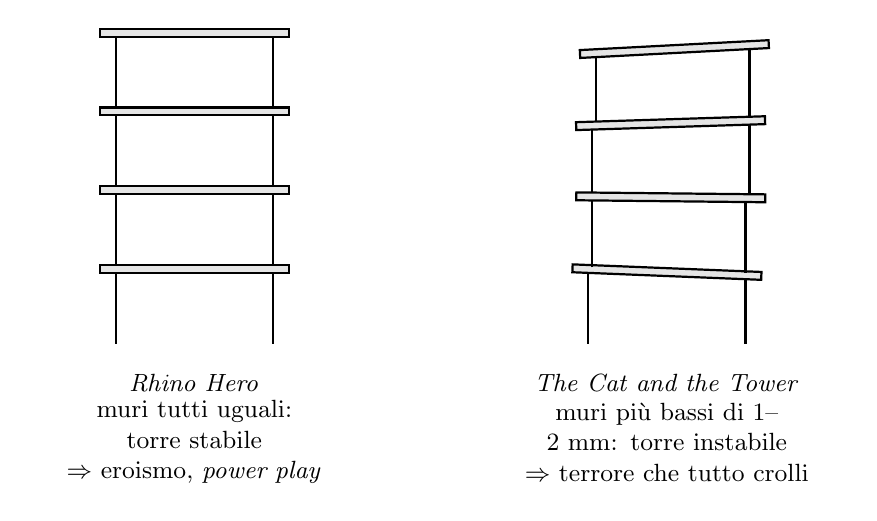
\begin{tikzpicture}[font=\small, x=1cm, y=1cm]
  % Rhino Hero: piani regolari
  \begin{scope}[shift={(0,0)}]
    \foreach \y in {0,1,2,3}{
      \draw[thick] (0,\y) -- (0,\y+0.9);
      \draw[thick] (2,\y) -- (2,\y+0.9);
      \draw[thick, fill=gray!20] (-0.2,\y+0.9) rectangle (2.2,\y+1.0);
    }
    \node[align=center] at (1,-0.5) {\emph{Rhino Hero}};
    \node[align=center, text width=4cm] at (1,-1.25)
      {muri tutti uguali: torre stabile\\$\Rightarrow$ eroismo, \emph{power play}};
  \end{scope}
  % Cat and Tower: muri di altezze diverse
  \begin{scope}[shift={(6,0)}]
    \draw[thick] (0,0) -- (0,0.9);   \draw[thick] (2,0) -- (2,0.82);
    \draw[thick, fill=gray!20, rotate around={-2.3:(0,0.9)}] (-0.2,0.9) rectangle (2.2,1.0);
    \draw[thick] (0.05,0.97) -- (0.05,1.82); \draw[thick] (2.0,0.9) -- (2.0,1.8);
    \draw[thick, fill=gray!20, rotate around={-0.6:(0.05,1.82)}] (-0.15,1.82) rectangle (2.25,1.92);
    \draw[thick] (0.05,1.92) -- (0.05,2.72); \draw[thick] (2.05,1.9) -- (2.05,2.78);
    \draw[thick, fill=gray!20, rotate around={1.8:(0.05,2.72)}] (-0.15,2.72) rectangle (2.25,2.82);
    \draw[thick] (0.1,2.82) -- (0.1,3.64); \draw[thick] (2.05,2.88) -- (2.05,3.78);
    \draw[thick, fill=gray!20, rotate around={3.0:(0.1,3.64)}] (-0.1,3.64) rectangle (2.3,3.74);
    \node[align=center] at (1,-0.5) {\emph{The Cat and the Tower}};
    \node[align=center, text width=4.4cm] at (1,-1.25)
      {muri più bassi di 1--2 mm: torre instabile\\$\Rightarrow$ terrore che tutto
      crolli};
  \end{scope}
\end{tikzpicture}
\caption{Stessa meccanica, paragame diverso: due torri di cartone. In \emph{Rhino Hero}
i piani sono regolari e la dinamica è quella dell'eroe che sale; in \emph{The Cat and
the Tower} alcuni muri sono di uno o due millimetri più bassi, e la torre, sempre
storta, trasmette paura e fragilità. Schema illustrativo, con le pendenze esagerate.}
\label{a10:fig:torri}
\end{figure}

% ---------------------------------------------------------------------
\section{Chiusura: ci si vede il 12}
\label{a10:sec:chiusura}

Mancano tre minuti, ``tempo per un'ultima domanda'', magari ``quella nell'angolino, un
po' timida''. Non arriva (``adesso non ce la faccio''). Gianmarco si smuta, ``il segnale
internazionale'' di chi sta per salutare, ma non ha domande; Ruggero lo invita
scherzosamente a dire anche solo ``cose stupide, tipo: oggi ho ucciso una mosca in
bagno''.

``Allora, gente, io vi saluto, e la lezione di oggi si conclude così.'' L'appuntamento è
\textbf{il 12}, con i \emph{pitch}: ``non fate scherzi, so che li avete, so che li potete
fare''. Al \emph{pitch} non ci sarà solo Ruggero: ci saranno anche \textbf{Beatrice} e
\textbf{Daniele}. ``Buona serata, buona cena, buon weekend.''

% ---------------------------------------------------------------------
\section*{Punti chiave del capitolo}
\addcontentsline{toc}{section}{Punti chiave del capitolo}

\begin{itemize}
  \item La \textbf{UX} è un primo strato tra la persona che si avvicina al gioco e
        l'ecosistema di regole: può essere ``un incredibile aiuto o un gigantesco
        ostacolo''. Regole perfette che non arrivano a chi gioca finiscono ``nel
        cestino''.
  \item I \textbf{quattro pilastri}: \textbf{immediatezza} (si capisce subito, senza
        sforzo: spade e scudi, il barile di petrolio, l'alloro dei punti vittoria),
        \textbf{efficienza} (un'azione complessa nel minor spazio: ``pesca una carta''),
        \textbf{memorabilità} (il +4 di \emph{Uno}, il simbolo di ``tappare'' di
        \emph{Magic}), \textbf{soddisfazione} (\emph{Parks}, \emph{Canvas}, \emph{Tiny
        Epic Mechs}). Sono indipendenti: le icone di \emph{Race for the Galaxy} sono poco
        immediate ma molto efficienti.
  \item Immediato per chi gioca abitualmente non vuol dire immediato per tutti; anche il
        \textbf{colore} fa parte del significato di un'icona.
  \item Il \textbf{wireframe} delle carte cambia durante il prototipo: togliere ciò che
        vale zero, ridurre il testo con le icone, spostare ciò che conta meno. Nei primi
        stadi: \textbf{carte funzionali, non carte belle}.
  \item \textbf{Accessibilità}: font per la dislessia, \emph{curb cut effect} (ciò che è
        più accessibile per qualcuno lo è per tutti), daltonismo da verificare con
        \textbf{Chromatic Vision Simulator}; i mancini e le carte a ventaglio.
  \item Il \textbf{paragame} estende al gioco il \textbf{paratesto}: tutto ciò che non è
        regole e non è fiction, ma incide sull'esperienza. I bordi sono zone grigie
        (i librogame, \emph{Lift It}).
  \item Le aree: \textbf{materialità} (legno, plastica, metallo, app, spessore e
        \emph{core} delle carte, \emph{standee}; clessidra contro timer),
        \textbf{formato} (font, misura delle carte, \emph{200 Word RPG}),
        \textbf{regolamento} (pagine, più libretti, video, glossario,
        \emph{playthrough}, \emph{play aid}), \textbf{scatola} (dall'armadio alla
        Kallax), \textbf{grafica e illustrazioni} (due mestieri diversi),
        \textbf{interfaccia analogica}, \textbf{ambiente} (il tavolo IKEA, il treno,
        \emph{Jenga} in aereo), \textbf{audio}, \textbf{contesto}, \textbf{lingua},
        \textbf{spazio urbano e ibridi digitali}, \textbf{inserti e setup}.
  \item Il paragame \textbf{incide sulle regole}: il formato limita la complessità
        delle regole, la clessidra cambia la tensione, la colonna sonora può essere una
        meccanica. Ai \emph{pitch} e alle revisioni Ruggero chiederà
        \textbf{``tantissimi perché''}.
  \item I casi studio vanno da \emph{Cuba Libre} (due regolamenti, diagrammi di flusso
        per i bot, brochure per fazione) a \emph{193 Days} (solo un mazzo), da
        \emph{Shenzhen I/O} (il manuale stampato) a \emph{Meltdown} (tessere di
        ghiaccio). Il test: ``\textbf{poteva essere di cartone?}''
  \item Il paragame non agisce direttamente sulle dinamiche: agisce sulle meccaniche
        (e sulla fiction), come tutto il design. Serve a far sì che \textbf{le intenzioni
        di design arrivino} a chi gioca, anche quando chi l'ha progettato non è al
        tavolo.
  \item Gli \textbf{inserti} non sono un dettaglio: nessuno ama il \emph{setup}, e un
        buon inserto lo accorcia. Il \emph{setup} si può anche rendere parte del gioco,
        nei giochi leggeri.
  \item \textbf{Ricerca e sviluppo} anche sul paragame: \emph{Rhino Hero} e \emph{The
        Cat and the Tower} hanno la stessa meccanica, ma muri di altezza diversa
        trasformano l'eroismo in terrore. \emph{Copy, transform, combine}, e
        \textbf{cross-modalità}.
\end{itemize}

%    % =====================================================================
%  Analog Game Design, lezione 11 — Il pitch dei progetti di gruppo.
%  Una lezione senza slide e senza lezione frontale: i tre gruppi del
%  corso presentano in tre minuti l'idea del gioco che svilupperanno
%  fino a dicembre, e i tre docenti (Daniele, Beatrice e Ruggero) fanno
%  domande, si ritirano a discutere in privato e poi restituiscono i
%  feedback. In apertura, l'attesa e le regole del pitch. Poi i tre
%  pitch, ciascuno con le sue domande: Murder Memory (escape room
%  investigativa da tavolo a squadre), La Peste (party game a ruoli
%  segreti ispirato alla Maschera della Morte Rossa), un gioco di ruolo
%  in solitario deck building, roguelike e journaling. Dopo la camera
%  di consiglio: la premessa ai feedback (indicazioni, non consigli; il
%  regolamento di massima per il 6 novembre), la domanda di Tiziana su
%  che cosa sia un regolamento in una escape room, i feedback gruppo
%  per gruppo con i casi studio assegnati, il legame tra obiettivo e
%  agency, il perché dei tre minuti, i giochi "generalisti". Infine le
%  domande aperte: scrivere il gioco per chi lo gioca senza di voi, la
%  curse of knowledge, la vergogna delle idee, e una lunga discussione
%  su roguelike, RNG e narrativa modulare (partire dalle emozioni, non
%  dai perk; le meccaniche come metafore; l'ortogonalità).
%  Fonte: trascrizione dell'undicesima lezione (AGD11) del corso breve
%  di Analog Game Design, seconda edizione: una lezione online di circa
%  tre ore, lunedì 12 ottobre 2026, condotta da Daniele con Beatrice e
%  Ruggero.
%  Pacchetti richiesti nel preambolo del libro (già presenti nel
%  main.tex): \usepackage{booktabs}, \usepackage{tikz} con
%    \usetikzlibrary{shapes.geometric,shapes.symbols,shapes.misc,
%      arrows.meta,positioning,calc,fit}
%  (le librerie vanno caricate nel preambolo, non nel capitolo).
%  Consigliati, come per gli altri capitoli: \usepackage[italian]{babel}
%  e \usepackage[T1]{fontenc} (il capitolo compila anche senza).
%
%  Collocazione nel libro: parte "Analog Game Design", undicesimo
%  capitolo (numerazione propria 2.11). Nel file principale del libro,
%  subito dopo il capitolo 2.10:
%
%    \input{AGD/AGD10_ux_design_e_paragame}
%    \input{AGD/AGD11_pitch_e_feedback}
%
%  Tutte le etichette di questo capitolo hanno il prefisso "a11:"
%  (a11:cap:..., a11:sec:..., a11:fig:..., a11:tab:...). Il capitolo è
%  autonomo: non contiene \ref verso altri capitoli.
%  Le figure e le tabelle sono ricostruzioni schematiche di quanto
%  detto a voce (la lezione non ha slide dei docenti), non copie delle
%  slide dei gruppi. Dove la trascrizione è troppo rovinata per
%  ricostruire un dettaglio (un nome di gioco, chi sta parlando), il
%  capitolo lo dice invece di inventarlo.
% =====================================================================

\chapter[Il pitch dei progetti di gruppo]{Il pitch dei progetti di gruppo: tre
giochi, tre minuti, e i feedback di chi li dovrà giocare}
\label{a11:cap:pitch}

Questa è l'\textbf{undicesima lezione} del corso di \textbf{Analog Game Design}, ed è
diversa da tutte le precedenti. ``Non abbiamo slide, non abbiamo una lezione, nel senso
di lezione frontale'': oggi è il giorno del \textbf{\emph{pitch}}, quello che Ruggero, a
fine della lezione sul paragame, aveva dato per certo come ``il 12'', che ``sta nella
pietra''. I tre gruppi di lavoro del corso presentano in \textbf{tre minuti} l'idea del
gioco che svilupperanno fino a dicembre; dopo ogni presentazione i docenti fanno
qualche minuto di domande, poi il gruppo esce dalla stanza virtuale e i docenti
discutono in privato. Quando tutti e tre i gruppi hanno presentato, la seconda metà della
lezione è dedicata ``solo ai feedback, esclusivamente ai feedback''.

I tre progetti sono molto diversi tra loro. Il primo, \textbf{\emph{Murder Memory}}, è
una \emph{escape room} investigativa da tavolo in cui due squadre, la polizia e un
indiziato che ha perso la memoria, risolvono enigmi in parallelo fino a un
interrogatorio finale. Il secondo, \textbf{\emph{La Peste}}, è un \emph{party game} a
ruoli segreti, di deduzione e \emph{bluff}, ambientato nel ballo della \emph{Maschera
della Morte Rossa} di Edgar Allan Poe: a ogni rintocco dell'orologio si balla, ci si
scambiano le carte e la malattia si diffonde. Il terzo è un \textbf{gioco di ruolo in
solitario}, \emph{deck building}, \emph{roguelike} e di \emph{journaling}: si
sopravvive il più a lungo possibile tenendo in equilibrio corpo, mente e status
sociale di un personaggio, e alla fine della partita resta la sua storia, da scrivere.

I feedback sono franchi, e i docenti lo dicono subito: non saranno ``consigli'' ma, dove
l'esperienza dice che un gruppo si sta infilando in un ``ginepraio troppo grosso per il
periodo di tempo che avete'', \textbf{indicazioni} precise (``non fate questo, fate
questo''). I temi che ritornano per tutti e tre i gruppi sono pochi e molto concreti:
\textbf{convergere} su un'idea e uno \emph{scope} realizzabili, \textbf{scrivere il
regolamento} (``il vostro gioco lo devono poter giocare altre persone che non sono
voi''), collegare l'\textbf{obiettivo} di chi gioca a ciò che fa \textbf{turno per
turno}, partire dalle \textbf{emozioni} e non dai bilanciamenti, e usare i
\textbf{casi studio} come strumenti di \emph{problem solving}, non come modelli da
copiare. Ogni gruppo riceve una lista di giochi da studiare, in tutto più di quindici
titoli (tabella~\ref{a11:tab:reference}). L'ultima parte della lezione, aperta alle
domande, diventa una lunga discussione su \emph{roguelike}, generazione casuale e
narrativa modulare, temi che due dei docenti praticano per mestiere.

La lezione è \textbf{online}, su Zoom, e si tiene \textbf{lunedì 12 ottobre
2026}\footnote{La data è quella fissata nella lezione precedente (``il 12 sta nella
pietra'', e ``lunedì'' sono i \emph{pitch}). In questa lezione Daniele ricorda che
Gianmarco ``di solito lunedì arriva un'ora dopo per motivi di lavoro''.}, presumibilmente
dalle 17 alle 20 come le altre: Daniele, che arriva ``da sei ore di lezioni'', ne fa
``altre tre di fila'' e a fine serata parla della sua ``nona ora''. La conducono insieme
i tre docenti del corso: \textbf{Daniele}, che scandisce i tempi, fa partire il timer e
gestisce la sala d'attesa; \textbf{Beatrice} (``Bea''); e \textbf{Ruggero}. Gli studenti
sono divisi in tre gruppi: \textbf{Tiziana}, \textbf{Angelo} e \textbf{Lorenzo L.}
(\emph{Murder Memory}); \textbf{Tancredi}, \textbf{Gianmarco} e \textbf{Lorenzo}
(\emph{La Peste})\footnote{Nel corso ci sono due Lorenzo, e la trascrizione li
distingue solo in un punto, quando Daniele presenta il primo gruppo come ``Tiziana,
Lorenzo L. e Angelo''. L'altro Lorenzo è nel gruppo di Tancredi e Gianmarco (``io sono
con Gianmarco e Lorenzo'', dice Tancredi). Il capitolo scrive ``Lorenzo L.'' per il
primo e ``Lorenzo'' per il secondo.}; \textbf{Giordano}, \textbf{Nicola} e
\textbf{Rita} (il \emph{roguelike} in solitario)\footnote{Il nome di Rita è storpiato in
``Verità'' (``Giordano, Nicola, Verità'') e in ``Piano'' (``Rita, Piano e Nicola''); il
contesto e un successivo ``ha ragione anche Rita'' lo rendono sicuro.}.

Tre avvertenze di lettura, le stesse dei capitoli precedenti. La prima: la trascrizione è
automatica e storpia moltissimi nomi. Ruggero diventa ``Ruger'', ``Rugger'',
``Brugger'' e ``Rugg''; \emph{Murder Memory} diventa ``Merd Memory'', ``Mordor
Memory'', ``Marder Memory'' e ``Mordere Memory''; \emph{Lupus in Tabula} è ``Lupus in
Fabula'', ``l'Opus in Fabula'' e ``l'upus in tabula''; \emph{Slay the Spire} è ``Slade
of Spire'', ``Slade Spire'', ``Zade Spyder'' e ``As Lady Spire 2''; \emph{Reigns} è
``Rains'', ``Rain'' e ``Reins''; \emph{The Quiet Year} è ``The Quiet Ear'', ``White
Tier'', ``quai tier'' e ``quietire''; \emph{Inhuman Conditions} è ``In Human
Condition'', ``Unicondition'' e ``Non è un Condition''; Tabletop Simulator è ``Temporal
Simulator'' e ``Voltoltor Simulator''. Dove la ricostruzione è sicura, o molto probabile,
il capitolo usa la forma corretta e lo segnala in nota la prima volta; dove non lo è,
riporta la forma della trascrizione e lo dice. La seconda: con tre docenti e dieci
studenti che parlano spesso uno sull'altro, la trascrizione quasi mai segnala chi sta
parlando, e in più punti ripete due volte la stessa frase (un artefatto del
riconoscimento vocale, che il capitolo ignora). Il capitolo attribuisce le frasi quando
il contesto lo rende chiaro (chi viene chiamato per nome, chi dice ``io sto creando un
\emph{roguelike}'', chi ha scansionato un libro) e resta generico altrimenti. La terza:
le slide dei gruppi non sono nella trascrizione; il capitolo ricostruisce i giochi da ciò
che i gruppi dicono a voce, nelle presentazioni e nelle risposte.

\paragraph{Come leggere questo capitolo.} I tre progetti sono descritti per come sono
stati presentati il 12 ottobre: idee in fase embrionale, con parti ``ancora da
definire'' che i gruppi stessi segnalano. Il capitolo non le completa e non le corregge:
riporta le domande che i docenti fanno, le risposte, e poi i feedback. Le figure
ricostruiscono gli schemi che emergono dal discorso (la procedura del \emph{pitch}, il
round della \emph{Peste}, il legame tra obiettivo e \emph{agency}, il calendario fino a
dicembre); le tabelle riassumono i progetti e i casi studio. Qua e là, dei paragrafi di
\textbf{approfondimento} collegano la lezione ai libri di game design di riferimento
(soprattutto \emph{The Art of Game Design} di Jesse Schell e \emph{A Theory of Fun} di
Raph Koster) e a qualche nozione di psicologia della comunicazione; sono segnalati come
tali e non fanno parte della lezione.

Il percorso del capitolo segue quello della lezione:
\begin{enumerate}
  \item l'attesa, la logistica e le \textbf{regole del \emph{pitch}} (sezioni
        \ref{a11:sec:attesa} e~\ref{a11:sec:regole});
  \item i tre \emph{pitch}, ciascuno con le sue domande: \emph{Murder Memory},
        \emph{La Peste}, il \emph{roguelike} di \emph{journaling} (sezioni
        da~\ref{a11:sec:murder} a~\ref{a11:sec:roguelike});
  \item dopo la camera di consiglio, la \textbf{premessa ai feedback} e la domanda su
        \textbf{che cos'è un regolamento} (sezioni \ref{a11:sec:premessa}
        e~\ref{a11:sec:regolamento});
  \item i \textbf{feedback} gruppo per gruppo, con i casi studio (sezioni
        da~\ref{a11:sec:fbmurder} a~\ref{a11:sec:reference});
  \item le \textbf{domande aperte}: il regolamento come strumento di test, la
        \emph{curse of knowledge}, la vergogna delle idee (sezioni
        \ref{a11:sec:testing} e~\ref{a11:sec:vergogna});
  \item la discussione su \textbf{\emph{roguelike}, RNG e narrativa modulare}, e la
        chiusura (sezioni da~\ref{a11:sec:rng} a~\ref{a11:sec:chiusura}).
\end{enumerate}

% ---------------------------------------------------------------------
\section{L'attesa: una ``quotina di ansia''}
\label{a11:sec:attesa}

I primi a collegarsi sono Angelo, Nicola, Lorenzo e Rita; Beatrice e Ruggero sono già
in stanza. Daniele ``arriva un attimino in ritardo perché sta chiudendo un'altra
lezione''. La prima domanda è quella di sempre, ``come state? come vi sentite oggi?'', e
la risposta di uno studente riassume l'umore della classe: ``leggermente preoccupato
per il \emph{pitch}, ma se no tranquillo''. ``Anch'io, è normale'', gli risponde
Beatrice: ``ogni presentazione ha una quotina di ansia''. Lei, dice, è ``molto curiosa''
e ``abbastanza fiduciosa che usciranno bellissimi \emph{pitch}'': ``non preoccupatevi,
siamo proprio in ascolto anche per darvi una mano dove possiamo''. Poi va a prendere
``il mio quadernino di appunti, così mi segno le cose''.

In attesa dei ritardatari, i docenti aprono come al solito lo spazio per le domande,
magari di chi ha recuperato la lezione precedente. Uno studente la sta finendo di
recuperare: ``è una figata pazzesca''. Ruggero conferma che ``sulla questione del
paragame c'è tantissimo da dire'' e spera che abbia dato ``qualche spunto''. Poi spiega
la logistica, che ``già dovreste sapere'': niente slide e niente lezione frontale; ``oggi
vediamo i vostri \emph{pitch} e dedichiamo il tempo a ciascun gruppo''. Si corregge
subito dopo un lapsus (``dedichiamo il gruppo a ciascun tempo. Chi può dirlo? Qualcuno
finirà nell'800, qualcuno finirà nel 2000''). L'idea è di dare ai gruppi dei feedback
``in base anche al vostro \emph{pitch}''.

Arriva Daniele, accolto con un ``grazie in fanfare'': viene ``da sei ore di lezioni''
(``e invece adesso guarda, ne fai altre tre di fila''; ``Madonna, Daniele, ci lasci le
penne. Non svenire''). È lui a segnare le presenze. Arriva Tiziana, poi Tancredi. Mentre
manda ``due messaggi di lavoro'', Daniele dà un consiglio organizzativo: decidete ``dietro
le quinte'' l'ordine di presentazione dei gruppi, altrimenti lo sceglieranno i docenti.
Un vincolo c'è già: il gruppo di \textbf{Gianmarco}, Tancredi e Lorenzo va lasciato per
ultimo, perché Gianmarco il lunedì arriva circa un'ora dopo per lavoro (``tra una
quarantina di minuti massimo''). Un altro vincolo arriva da una studentessa del primo
gruppo, che deve staccarsi dieci minuti prima per prendere il treno delle otto: il suo
gruppo, se i compagni sono d'accordo (``Sì, sì, va bene''), può andare per primo. E
così si fa: ``iniziamo voi''.

Nel frattempo, il silenzio. ``Avremo l'\emph{horror vacui}'', scherza Ruggero: ``se
nessuno fa domande, io non so gestire. Daniele, cosa devo fare? Come faccio?''. Mancano
soltanto Giordano e Gianmarco; Daniele chiede di avvisarlo se entrano mentre i gruppi
presentano, così da non perdere le loro presenze.

C'è un ultimo intoppo tecnico, quello di ogni lezione online: la condivisione dello
schermo da un Mac (``il problema sempre del Mac per le autorizzazioni''). Daniele
sospetta un aggiornamento di Zoom (``e l'aula è diversa, tra l'altro: voi non ve ne
rendete conto, ma è un'aula differente''), ma alla fine la presentazione del primo
gruppo parte, in modalità ``presenta'', a schermo intero, con le frecce della tastiera
per andare avanti.

% ---------------------------------------------------------------------
\section{Le regole del \emph{pitch}}
\label{a11:sec:regole}

Prima di cominciare, Daniele ripete ``bene le regole del \emph{pitch} di oggi''
(figura~\ref{a11:fig:procedura}).

\begin{itemize}
  \item \textbf{Tre minuti.} Daniele fa partire un timer, conta ``3, 2, 1, via'', e il
        gruppo spiega ``tutto''. Chi va oltre non viene interrotto (``vi faccio
        finire''), ma alla fine si sentirà dire se è andato ``troppo lungo'' o ``troppo
        corto'', ``perché comunque sapevate che più o meno il tempo era quello''. Il
        tempo è uguale per tutti: ``non possiamo dare la possibilità a ogni team di
        avere più tempo rispetto agli altri. Altrimenti, è un casino''.
  \item \textbf{Due o tre minuti di domande} da parte di Daniele, Ruggero e Beatrice
        (``comunque quanto tempo ci mettono'').
  \item \textbf{La sala d'attesa.} Il gruppo esce da Zoom e rientra: Daniele ha
        attivato la sala d'attesa. I tre docenti si prendono ``qualche appunto in
        privato di confronto, senza essere registrati'', e poi riammettono tutti.
        Quando una studentessa chiede se la sala d'attesa sia ``una stanza che c'è
        veramente'', la risposta è che è ``l'anticamera'' di Zoom, dove però non si
        può parlare: chi vuole chiacchierare nel frattempo ha un canale vocale
        ``Analog Game Design'' sul Discord del corso.
  \item Si fa così per tutti i gruppi. La parte dei \emph{pitch} ``di solito dura
        un'ora, un'ora e mezza''; poi ``vi diamo i feedback e vi diamo anche dei
        consigli su cosa fare, perché poi dovrete svilupparle, 'ste robe''.
  \item \textbf{Il materiale.} Dopo ogni presentazione il gruppo condivide in chat il
        link alle slide (``Condividi'', ``chiunque abbia il link'', copia, incolla) e
        carica tutto nella cartella \emph{project work} del proprio gruppo.
\end{itemize}

Il primo gruppo avverte che improvviserà (``non ci siamo preparati sulla
presentazione''). Nessun problema, ma conviene che parli una persona sola, se ne ha una
che ``sa tutto quanto''; gli altri intervengono se manca qualcosa. Le domande dei
docenti, durante il primo \emph{pitch}, si allungano: alla fine il primo gruppo occupa
venti minuti, e Daniele stabilisce per gli altri ``venti minuti più o meno a team''.
Nessun feedback a caldo, nemmeno per chi deve andarsene prima: i docenti vogliono prima
``vedere il livello di tutti'', ``cosa hanno prodotto tutti''.

\begin{figure}[htbp]
\centering
\begin{tikzpicture}[
  font=\small,
  a11step/.style={draw, thick, rounded corners=3pt, minimum height=1.2cm,
               text width=2.3cm, align=center},
  a11priv/.style={draw, thick, dashed, rounded corners=3pt, fill=gray!15,
               minimum height=1.2cm, text width=2.3cm, align=center},
  a11arr/.style={-{Stealth[length=3mm]}, thick}
]
  \node[a11step] (a) {\textbf{Pitch}\\3 minuti\\a timer};
  \node[a11step, right=0.6cm of a] (b) {\textbf{Domande}\\2--3 minuti\\dei docenti};
  \node[a11priv, right=0.6cm of b] (c) {\textbf{Sala d'attesa}\\appunti dei\\docenti, non
    registrati};
  \node[a11step, right=0.6cm of c] (d) {\textbf{Rientro}\\e prossimo\\gruppo};
  \draw[a11arr] (a) -- (b);
  \draw[a11arr] (b) -- (c);
  \draw[a11arr] (c) -- (d);
  \draw[a11arr, rounded corners=4pt] (d.south) -- ++(0,-0.7) -| node[pos=0.25, below,
    font=\footnotesize]{per ognuno dei tre gruppi (circa 20 minuti a gruppo)} (a.south);
  \node[a11step, below=1.9cm of c, text width=5.2cm, fill=gray!5] (f)
    {\textbf{Seconda metà della lezione}\\feedback di gruppo, feedback di classe,
     domande aperte};
  \draw[a11arr, dashed] (d.east) -- ++(0.4,0) |- (f.east);
\end{tikzpicture}
\caption{La procedura del \emph{pitch} come la descrive Daniele. I feedback non arrivano
a caldo: i docenti li danno solo dopo aver visto tutti e tre i gruppi.}
\label{a11:fig:procedura}
\end{figure}

\paragraph{Approfondimento: il \emph{pitch} come prova di comunicazione.} Il formato
non è arbitrario, e Daniele lo spiegherà più avanti (sezione~\ref{a11:sec:fbpeste}):
tre minuti sono più o meno il tempo che un editore o un passante in fiera concede a
un'idea. Ma il \emph{pitch} è anche il primo momento in cui il gioco esce dalla testa del
gruppo e arriva a qualcuno che non c'era quando è stato pensato. Schell, in \emph{The Art
of Game Design}, dedica a questo passaggio un capitolo intero (``The Designer Gives the
Client a Pitch''), con l'idea di fondo che presentare un gioco serve anche a chi lo
presenta: costringe a scegliere che cosa, del gioco, conta davvero. Le domande dei docenti che seguono ogni \emph{pitch} di questa lezione
sono, in gran parte, la verifica di questo: che cosa faccio, io che gioco, in questo
momento?

% ---------------------------------------------------------------------
\section{Primo \emph{pitch}: \emph{Murder Memory}}
\label{a11:sec:murder}

Il primo gruppo è quello di \textbf{Tiziana}, \textbf{Lorenzo L.} e \textbf{Angelo}.
Presenta Tiziana, con l'accordo dei compagni, che interverranno se lei dimentica
qualcosa. Beatrice è ``già curiosissima di questo \emph{Murder Memory}'', e quando
lascia scappare un ``ho visto che è un gioco di carte'' viene fermata: ``non ci si
spoilera''. ``3, 2, 1, via.''

\subsection{Il \emph{pitch}}

\emph{Murder Memory} è ``una \emph{escape room} investigativa da tavolo'' (``ci siamo
dimenticati di precisare questa cosa, ma sarà da tavolo''). Chi gioca si trova coinvolto
in una \textbf{festa nella villa di un ricco proprietario}, durante la quale uno degli
invitati viene ucciso. Il principale indiziato è un altro invitato, che ha perso i sensi
e si sveglia \textbf{senza memoria}.

È un gioco \textbf{competitivo e cooperativo} insieme: due squadre si affrontano per
arrivare alla verità entro un \textbf{tempo limitato}, cooperando al loro interno.
\begin{itemize}
  \item Una squadra interpreta l'\textbf{indiziato} che ha perso la memoria. Non ricorda
        chi è né che cosa sia successo; potrebbe essere l'assassino e non saperlo. Si
        nasconde dalla polizia mentre cerca la verità, il che lo rende ancora di più il
        principale indiziato. ``Enigma dopo enigma'' deve scoprire chi è e svelare il
        mistero: ``è davvero lui il colpevole, o è solo un'altra vittima?''. Ogni
        giocatore della squadra potrebbe interpretare \textbf{un aspetto diverso della
        stessa persona}: è una cosa ``ancora da definire'', perché il gruppo non sa
        ancora se riuscirà a realizzarla in concreto.
  \item L'altra squadra interpreta i \textbf{poliziotti}, chiamati dal proprietario.
        Seguono le indagini, cercano indizi e interrogano gli invitati e il
        proprietario della villa, anche a proposito dell'indiziato che non riescono a
        trovare.
\end{itemize}

La struttura è una \textbf{successione lineare di enigmi}, che guida ciascuna squadra
alla risoluzione finale; la risoluzione prevede un \textbf{confronto diretto} tra le due
squadre, attraverso un \textbf{interrogatorio}. Il gruppo vorrebbe diversificare il più
possibile gli enigmi della successione, così da far partecipare più giocatori.
L'obiettivo dell'indiziato è scoprire la verità su se stesso e su ciò che è successo;
quello dei poliziotti, trovare il colpevole.

L'obiettivo del gruppo, come designer, è ``esprimere noi stessi ed esplorare nuove
tipologie di gioco'', fondendo elementi investigativi e di gioco di ruolo con la
struttura dell'\emph{escape}; e ``non ci dispiacerebbe pubblicarlo''. Le
\textbf{emozioni} che vogliono suscitare sono \textbf{incertezza}, \textbf{scoperta},
un'esperienza \textbf{adrenalinica}, \textbf{sorpresa} e \textbf{ansia}. Chiude una
battuta (``prenotatevi per provarlo, nessuno vi picchierà'') e la presentazione dei
membri del gruppo, ognuno con un nome da personaggio\footnote{La trascrizione riporta
``siamo Lorenzo, la Pomarda, Angelo, Tenente Colombo e io, Tiziana Carabayt'': almeno
``Tenente Colombo'' è chiaramente un soprannome scherzoso a tema investigativo; le
altre parole non sono ricostruibili con sicurezza.}.

Tempo: \textbf{tre minuti e quattordici secondi}. ``Direi che siamo comunque in
\emph{time}'', commenta Daniele: con un po' più di velocità ci sarebbero stati
tranquillamente.

\subsection{Le domande}

\paragraph{Come si vince?} Daniele parte con un apprezzamento e un dubbio. ``Lato
emotivo, molto bene'': le emozioni sono chiare. ``Lato meccanico, ho un po' di dubbi.''
Non è chiaro se il gioco abbia un \textbf{\emph{endgame} predefinito}, cioè se a livello
meccanico si vinca o si perda (``com'è che so se ho vinto o se ho perso?''), o se vada
``nella direzione più RPG'', in cui conta non chi vince ma ``avere un epilogo
strutturato''.

\paragraph{Chi risolve gli enigmi?} Un'altra domanda, più pragmatica, arriva dai docenti
insieme: le squadre sono due, ma gli enigmi chi li risolve? Insieme? Una squadra sola
mentre l'altra aspetta? (``Hanno due serie diverse.'') Il punto, chiarisce chi chiede, è
che non è chiaro ``che cosa faccio, in base al ruolo in cui sono'', e con quale obiettivo
personale al tavolo. Gli studenti non sapevano se dovessero entrare in questo dettaglio
nel \emph{pitch}; la risposta dei docenti è: se la risposta c'è, ditela; se non c'è,
``non generatela adesso''.

La risposta c'è. Gli enigmi procedono \textbf{in contemporanea}, con lo stesso tempo per
entrambe le squadre. I poliziotti hanno tutte le informazioni se riescono ad arrivare
alla fine del loro percorso; l'indiziato, arrivando alla fine del suo o il più vicino
possibile, ottiene informazioni su se stesso. \textbf{Allo scadere del tempo} le due
squadre si confrontano: i poliziotti fanno all'indiziato delle domande ``ovviamente
previste'', e l'indiziato saprà rispondere più o meno correttamente a seconda di quanto
ha scoperto. Se non sa chi è, ``rischia di rimanere un po' così'' su certe domande:
può inventarsi le risposte, ma rischia di non essere coerente. Ne nascono diversi esiti
(tabella~\ref{a11:tab:esiti}).

\begin{table}[htbp]
\centering
\small
\begin{tabular}{@{}p{5.6cm}p{7.4cm}@{}}
\toprule
\textbf{Situazione allo scadere del tempo} & \textbf{Esito (come descritto nel
\emph{pitch})} \\
\midrule
Entrambe le squadre arrivano alla fine del percorso & ``vincono entrambi'': i
poliziotti hanno gli elementi per capire chi è il vero colpevole, e l'indiziato sa
rispondere \\
I poliziotti arrivano alla fine, l'indiziato no & vincono i poliziotti: l'indiziato non
risponde correttamente alle domande e viene arrestato \\
L'indiziato ottiene le informazioni su di sé & l'indiziato vince: risponde correttamente
e viene scagionato \\
\bottomrule
\end{tabular}
\caption{Gli esiti dell'interrogatorio finale di \emph{Murder Memory}, come li descrive
Tiziana rispondendo alle domande. Il gruppo li presenta come idea ancora aperta.}
\label{a11:tab:esiti}
\end{table}

\paragraph{Quanti giocatori?} Daniele ha ``due domande molto brevi''. La prima: per
quanti giocatori è il gioco? Minimo due, uno per squadra; il gruppo pensava a un massimo
di \textbf{quattro per squadra}. Si interpretano solo i membri delle squadre? Sì: gli
invitati sono \textbf{NPC}. La seconda domanda, a Daniele, sfugge (``la sto perdendo?
Arrivo''); Beatrice lo rassicura (``è normale, poi tornano le domande mentre si
parla'') e prende la parola.

\paragraph{L'indiziato vuole scagionarsi o sapere la verità?} Beatrice ha ``tantissime
domande'' e ne seleziona alcune. La prima: la squadra dell'indiziato ha più lo scopo di
scagionarsi o di ricostruire la verità? Deve scoprire la verità su se stesso, risponde
Tiziana: scoprendo chi è, può affrontare i poliziotti. Beatrice chiede allora conferma
di un punto di design: si parte dall'idea che l'indiziato \textbf{non è colpevole}?
Corretto: non è colpevole, ``però non lo sa''.

\paragraph{Le sfaccettature dell'indiziato.} La seconda domanda di Beatrice riguarda le
``varie modalità di essere'' dell'indiziato, una per giocatore. Come funzionerà? Il
dubbio di Beatrice è più ampio: ``avete tanta carne al fuoco''. Enigmi, \emph{drive}
narrativi, una storia raccontata in più versioni, una polizia che non è una persona sola.
``Non vi sto invitando per forza a ridurre lo \emph{scope}'', ma ``è bene che abbiate una
direzione e una motivazione per tutte le scelte che prendete''. L'idea dell'indiziato
interpretato da una squadra intera le piace molto, ma non capisce che cosa farà lei,
giocando l'indiziato, oltre al lavoro di ricerca con le altre parti di sé: e quando
dovrà scagionarsi, come funzionerà? ``Compileremo una scheda, oppure parleremo con la
polizia?''. La risposta: la \textbf{mente divisa} era un'ipotesi iniziale, ``quasi
necessaria'' per giustificare più persone che fanno un'unica persona, ma non
obbligatoria, perché ``è nostra intenzione semplificare, non complicarci la vita''.

\paragraph{``Dovete spoilerare''.} A questo punto il gruppo ammette che manca una parte,
taciuta apposta ``perché non volevamo spoilerare''. La reazione dei docenti è immediata:
``Dovete spoilerare. Non siamo giocatori''. Al \emph{pitch} i docenti sono come un
\emph{publisher} a cui si propone un gioco: se non gli si dicono le cose importanti,
``noi come facciamo?''. ``Non lo sapevamo. Scusate.'' ``Tutto bene. Dici tutto adesso.''

Il retroscena è questo. Il \textbf{proprietario} della villa è un \textbf{appassionato di
enigmi} ed è lui \textbf{l'assassino}: ha ucciso uno degli invitati per costruire tutta
la messa in scena, ``fondamentalmente per divertirsi''. È lui a far perdere la memoria
all'indiziato, facendogli bere qualcosa. L'indiziato si sveglia in un punto in cui non è
visto, si accorge che è successo qualcosa (c'è la polizia) e va subito in agitazione:
non ricorda chi è, e se gli fanno una domanda non saprà cosa rispondere. Mentre si
nasconde trova \textbf{un oggetto che gli è familiare}, e da lì parte la serie degli
enigmi. Ha la sensazione di essere \textbf{guidato}, pilotato, che ci sia qualcosa che
non torna, ma ``non è il momento'' di chiederselo. Dall'altra parte, il proprietario
chiama i poliziotti e si diverte anche alle loro spalle: li guida attraverso altri
enigmi, con cui ricostruiscono le informazioni sugli invitati e, attraverso gli invitati,
sull'indiziato che non trovano. ``Scusa, no, è importantissimo'', commentano i docenti.

\paragraph{Storia prefatta o emergente?} Daniele fa un'ultima domanda, ``molto
semplice'': il gioco ha una \textbf{storia prefatta}, definita, che i giocatori stanno
solo scoprendo? Non è una storia emergente? Sì, è prefatta.

\paragraph{I giochi più vicini.} Poi tocca a Ruggero, con una domanda ``apparentemente
dal nulla'', le cui ragioni verranno dette dopo: nella fase di ricerca e sviluppo, quali
sono i giochi più vicini al vostro? Ruggero ne ha già ``due segnati qua'' che ``devono
uscire fuori da questa risposta''. Non è un indovinello, precisa: se i giochi citati dal
gruppo coincidono con i suoi, bene; se sono molto diversi, ``allora ci sono altri
problemi'', perché vuol dire che i docenti hanno capito un'altra cosa. Daniele allarga
la domanda: non serve un gioco unico che spieghi tutto il progetto, che ibrida generi
diversi ed è in gran parte sperimentale (``è molto chiaro quello che ci state
proponendo''); bastano ``un po' di ispirazioni'', e la ricerca e sviluppo ``può essere un
film, può essere una canzone''.

Tiziana racconta l'origine dell'idea: il gruppo ha scelto la proposta di Lorenzo L., un
personaggio che perde la memoria e cerca di ricostruirla, e poi l'interesse comune per
le scelte, per l'\emph{escape} e per gli elementi investigativi. Lei ha cercato giochi
simili ``e non ho trovato niente''; ha giocato investigativi e qualche \emph{escape}, ma
non si è ispirata a nessuno in particolare (``se ci volete dare qualche indicazione,
siamo contenti''). Aggiunge un'idea sua sul formato: dare i percorsi ``in modalità
busta'', con buste da aprire che contengono il testo scritto; ma nel gruppo c'è chi ha
un'idea diversa. ``Quello lo svilupperete dopo''. Lorenzo L., invece, un riferimento ce
l'ha: quando aveva proposto la perdita di memoria, gli era venuto subito in mente un
titolo della serie \textbf{\emph{Hidden Games}}, in cui tutti hanno perso la memoria,
tutti indagano e uno di loro è l'assassino: \emph{Freddo come il
ghiaccio}\footnote{Così nella trascrizione (``Freddo come il ghiaccio. Bravissimo,
Lorenzo''). \emph{Hidden Games} è una serie di giochi investigativi in scatola; il
titolo esatto del caso citato non è verificabile dalla trascrizione.}. ``Bravissimo,
Lorenzo.'' Angelo, a parte le \emph{escape room} giocate (``non particolarmente
tante''), non ha riferimenti: è proprio questo che lo ha spinto ad avvicinarsi al genere.

Sono passati venti minuti, ed è arrivato Gianmarco. Daniele riassume per lui la
procedura (presentazione, domande, sala d'attesa, feedback alla fine) e manda il primo
gruppo in sala d'attesa.

% ---------------------------------------------------------------------
\section{Secondo \emph{pitch}: \emph{La Peste}}
\label{a11:sec:peste}

Visto che Gianmarco è arrivato, il secondo turno tocca al suo gruppo: \textbf{Tancredi},
\textbf{Gianmarco} e \textbf{Lorenzo}. Presenta Tancredi. Prima di partire, però, c'è un
equivoco da chiarire: il gruppo ``non si era orientato per i tre minuti''. Aveva capito
che il \emph{pitch} fosse ``una cosa un po' più lunga'', e ha preparato una struttura ``un
po' più cicciotta'', poi riadattata con alcune slide in appendice. ``Sapevate quanto tempo
ci davamo?'' ``Noi avevamo trenta minuti.'' Daniele si chiede se sia stata colpa sua, ma
ricorda di essere stato chiaro: ``i \emph{pitch} erano da tre minuti, tre o quattro minuti
di solito''. Gli studenti stessi trovavano strano un \emph{pitch} così lungo (``come idea
avevamo tutti in mente un \emph{pitch} che fosse una roba molto veloce''). Il materiale in
più non va buttato: ``tenetelo da parte, che servirà''. E il gruppo, alla fine, sta nei
tre minuti: ``bravissimi''.

\subsection{Il \emph{pitch}}

Il gioco si chiama \textbf{\emph{La Peste}} ed è ambientato nel racconto \emph{La
maschera della Morte Rossa} di Edgar Allan Poe (``ce la posso fare''). È un \textbf{party
game a ruoli segreti}, di \textbf{deduzione e \emph{bluff}}. Uno degli invitati del ballo
rappresenta la malattia, che il gruppo chiama \textbf{Pestilenza}, e il suo obiettivo è
espandersi. A ogni \textbf{rintocco dell'orologio} (scandito da un piccolo timer, che
definisce i round) ci si mette a \textbf{ballare}: durante il ballo i giocatori si
scambiano le carte, e in base alle carte che si hanno in mano alla fine del turno si è
sani o malati. Dopo il ballo c'è la \textbf{fase sociale}, ``quella un po' più caciarona
da \emph{party game}'', in cui ci si accusa e si cerca di capire chi si è ammalato e chi
no.

I \textbf{pilastri} del gioco sono tre: la \textbf{dualità segreta} tra Pestilenza e
Medico, che si combattono senza che nessuno sappia chi sono; la \textbf{malattia che si
espande}; la \textbf{deduzione e il \emph{bluff}}. Le \textbf{emozioni} principali sono
l'\textbf{incertezza} (non sapere bene i ruoli), l'\textbf{ansia} e la
\textbf{preoccupazione}, e l'\textbf{inclusione}: i giocatori malati \textbf{non vengono
eliminati}, come invece ``ogni tanto succede nei giochi di questo tipo''. Il formato è da
\textbf{5 a 8 giocatori}, per circa \textbf{30 minuti} (``ancora un po' da decidere'').

I ruoli sono tre (tabella~\ref{a11:tab:ruoli}). Il \textbf{setup} è a \textbf{buste},
come in \emph{Secret Hitler}\footnote{Nella trascrizione ``Secret Teaser'', poi
``Secreti Hitler''.}: ogni busta è già preparata in base al numero di giocatori e
contiene le carte di chi la riceve. Il gioco si sviluppa in \textbf{sette round}, il
numero dei rintocchi (``va ancora sistemato''); ogni round ha tre fasi: il
\textbf{ballo}, in cui ci si scambiano le carte; la \textbf{risoluzione}, in cui in base
alle carte che si hanno ``succedono cose'' (``tendenzialmente ti ammali''); la
\textbf{fase sociale}, la discussione. Alla fine si guardano le \textbf{condizioni di
vittoria} (figura~\ref{a11:fig:round}).

\begin{table}[htbp]
\centering
\small
\begin{tabular}{@{}p{2.4cm}p{4.6cm}p{6cm}@{}}
\toprule
\textbf{Ruolo} & \textbf{Carte iniziali} & \textbf{Obiettivo e comportamento} \\
\midrule
Pestilenza & una carta \emph{peste}, che trasmette la malattia, e una carta vuota &
l'unico che parte malato; vuole contagiare tutti \\
Medico & due \emph{talismani}, che proteggono dalla malattia (``non ti fa ammalare'') &
combatte la Pestilenza senza farsi riconoscere \\
Cortigiani & solo carte vuote (\emph{invito}) & finché sono sani giocano con il Medico;
quando si infettano passano dalla parte della Pestilenza e vogliono far infettare
tutti \\
\bottomrule
\end{tabular}
\caption{I ruoli della \emph{Peste} come presentati al \emph{pitch}. Le carte vuote,
nella descrizione del \emph{setup}, si chiamano ``invito''.}
\label{a11:tab:ruoli}
\end{table}

\begin{figure}[htbp]
\centering
\begin{tikzpicture}[
  font=\small,
  a11ph/.style={draw, thick, rounded corners=3pt, minimum height=1.2cm,
             text width=2.6cm, align=center},
  a11arr/.style={-{Stealth[length=3mm]}, thick}
]
  \node[a11ph, fill=gray!10] (s) {\textbf{Setup}\\buste preparate per numero di
    giocatori};
  \node[a11ph, right=1.0cm of s] (b) {\textbf{Ballo}\\si scambiano le carte};
  \node[a11ph, right=0.7cm of b] (r) {\textbf{Risoluzione}\\sani o malati, in base alle
    carte in mano};
  \node[a11ph, below=1.3cm of r] (f) {\textbf{Fase sociale}\\accuse, discussione,
    deduzione};
  \node[a11ph, right=1.0cm of f, fill=gray!10] (v) {\textbf{Fine}\\condizioni di
    vittoria};
  \draw[a11arr] (s) -- node[above, font=\footnotesize]{rintocco} (b);
  \draw[a11arr] (b) -- (r);
  \draw[a11arr] (r) -- (f);
  \draw[a11arr] (f.west) -| node[pos=0.25, below, font=\footnotesize]{prossimo
    rintocco (7 in tutto)} (b.south);
  \draw[a11arr, dashed] (f) -- node[above, font=\footnotesize]{dopo il
    7\textsuperscript{o}} (v);
\end{tikzpicture}
\caption{Il ciclo di gioco della \emph{Peste} come descritto al \emph{pitch}: sette
round, uno per rintocco dell'orologio, ciascuno con ballo, risoluzione e fase sociale.
Il numero di round è ancora da sistemare.}
\label{a11:fig:round}
\end{figure}

Il \textbf{target} è pensato per una serata in cui il gioco viene ``intavolato'' da una
persona, magari ``quella un po' più giovane'', fan di questa categoria di giochi:
l'appassionato di \emph{Lupus in Tabula}, che non conosce \emph{La Peste} ma sicuramente
la apprezzerà, perché il genere gli piace. Accanto a lui, due target più
\emph{casual}: chi non ha mai giocato e si sta avvicinando ai giochi da tavolo per la
prima volta, e chi ``subisce il gioco'', perché non sapeva che quella sera si sarebbe
giocato.

Tempo: \textbf{due minuti e cinquantotto secondi}. Tancredi aggiunge una cosa che stava
nelle slide in appendice: una \textbf{variante interpretativa}, che al gruppo piacerebbe
molto, perché potrebbe aiutare a sdrammatizzare, ma che rischia anche di rendere il
gioco ``un po' più caotico''.

\subsection{Le domande}

Daniele chiede, come sempre, il link alle slide e il caricamento nella cartella
\emph{project work} (``c'è tutto, sia la versione \emph{full} che la versione tagliata'').
Poi la prima domanda, ``la mia classica'': quali titoli di riferimento avete osservato?
``Secret Hitler e Lupus in Tabula: quelli sono già ovvi.'' Non sono nelle slide, ma ce
ne sono vari.

\paragraph{I cortigiani possono difendersi?} Beatrice fa una domanda ``forse prematura'':
il Medico ha due carte per difendersi; i cortigiani, se si beccano la carta peste, hanno
qualche arma? Per ora no. Il Medico, anzi, potrebbe essere immune: va testato quanto è
forte. Si potrebbe dargli una sorta di protezione propria, ``come se avesse già un
talismano per sé''. E c'è un'altra meccanica a cui il gruppo ha pensato: se un giocatore
si ritrova con \textbf{due talismani}, \textbf{diventa anch'esso un Medico}. Ne nasce una
tensione interessante: c'è chi non vuole cedere il proprio talismano per paura, ``però
meno lo fai girare, meno aiuti i compagni'', e così, senza volerlo, aiuta la Pestilenza
a espandersi. ``Molto bene.''

\paragraph{Si può giocare senza componenti?} Ruggero, per ora, non ha domande. Daniele
ne fa una ``fuori dai denti'': questo gioco si potrebbe intavolare senza nessuna
componente materiale, come un \emph{Lupus in Tabula} di base, o il gruppo pensa a un
formato speciale? Le carte servono, risponde il gruppo, insieme a una scatola e a dei
componenti. E una versione da LARP, in costume? Ci hanno ragionato, ma l'idea è giocarlo
al tavolo, seduti, con le carte.

\paragraph{Le buste.} Ultima domanda di Daniele: come si gestiscono le buste nel
\emph{setup}? Ogni busta conterrà la carta ruolo e le carte di gioco (``talismano,
talismano, peste, invito, invito, invito''). Manca ancora la parte su come comporre le
buste a seconda del numero di giocatori, che ``cambieranno''. Beatrice ha altre domande,
ma le terrà per la discussione privata dei docenti. Il gruppo va in sala d'attesa
(``ci vediamo qua fra pochissimo'').

% ---------------------------------------------------------------------
\section{Terzo \emph{pitch}: un \emph{roguelike} di \emph{journaling} in solitario}
\label{a11:sec:roguelike}

Mentre gli altri rientrano arriva \textbf{Giordano}, che è stato aggiornato sulla
struttura della lezione dai compagni ``mentre stavo tornando a casa''. Il suo gruppo,
con \textbf{Nicola} e \textbf{Rita}, è l'ultimo. Presenta Nicola, che condivide l'intero
schermo e avverte: ``a differenza degli altri'' il gruppo ha raccolto tutto ``all'interno
di una singola slide''. ``Non c'era l'obbligo di più slide, non ti preoccupare.''

\subsection{Il \emph{pitch}}

Il gioco è un \textbf{gioco di ruolo in solitario} e un \textbf{\emph{deck building
game}}. A differenza di molti giochi che vanno su approcci da librogame (``pagina X,
pagina Y''), il gruppo ha voluto creare un \textbf{\emph{loop} di gioco rigiocabile},
adatto a due tipi di persone: chi vuole avvicinarsi al gioco di ruolo da solo, ``con la
comodità di casa sua, senza avere paura delle altre persone''; e il giocatore di ruolo
``molto avanzato'', che vuole facilitare la \textbf{creazione del proprio personaggio}
attraverso una storia dinamica.

Le ispirazioni dichiarate sono \emph{Slay the Spire} e \emph{Reigns}: ci si trova di
fronte a delle \textbf{situazioni}, si risponde con delle \textbf{carte} e si devono
tenere in equilibrio alcune \textbf{statistiche della vita} del personaggio, per esempio
lo \textbf{stato fisico} del corpo, lo \textbf{stato della mente} e lo \textbf{status
sociale}. Il giocatore è uno solo. Il gioco è pensato per essere \textbf{facilmente
espandibile} con nuovi ``settori'': la prima versione ha un'\textbf{ambientazione
moderna}, in cui si interpreta ``X persona, senza genere, per essere inclusivo verso
chiunque''.

All'inizio si fa la prima pescata di carte, che assegna al personaggio dei
\textbf{tratti casuali}: il personaggio può essere irascibile, con certi bonus e malus in
certe situazioni, oppure può avere la malaria, con altri bonus e malus. Bisogna
\textbf{sopravvivere} e andare ``il più possibile lontano'', fino a quando una delle
barre si esaurisce. La morte può essere \textbf{fisica} (il corpo non ce la fa più,
magari perché il personaggio è stato ``un fumatore incallito per tutto il tempo''),
\textbf{mentale} (impazzisce) o \textbf{sociale} (``non riesce più a sopportarsi
all'interno del mondo''). L'ambientazione è moderna, ma il sistema è pensato come
\textbf{\emph{setting agnostic}}: ``l'obiettivo è stato il \emph{loop} di gioco''.

Chi gioca può anche non affrontare il lato narrativo, ma sarebbe ``desiderato'', perché
l'obiettivo è incitare al \textbf{\emph{journaling}}: quando la partita finisce, con la
morte del personaggio, si ha già la sua storia scritta, e si può fare
\emph{journaling} dal punto di vista narrativo, oppure usarla per imparare a fare una
\emph{run} migliore e arrivare più lontano.

Sui \textbf{componenti}: carte personalizzate, ma se stamparne ``un numero gigantesco''
dovesse essere un problema, il gruppo pensa di usare un \textbf{mazzo di carte
francesi}, in cui seme, valore e carta determinano se si tratta di una situazione, di un
evento o di una carta da giocare. I tratti sono casuali all'inizio, e altre carte si
aggiungono durante la partita. ``Fine.''

Tempo: \textbf{tre minuti precisi}.

\subsection{Le domande}

Ruggero aveva già ``elencato i giochi ispirati'' e non ha domande, ma ha ``un po' di cose
su cui sto ragionando''. Lascia la parola a Beatrice e a Daniele.

\paragraph{Quali emozioni?} Beatrice cercava nella slide le emozioni e non le ha trovate.
La risposta del gruppo: la \textbf{curiosità} di sapere che cosa c'è dopo, di andare
avanti, e la \textbf{competizione} con se stessi, il portare ``uno \emph{score} sempre
migliore'': ``alla fine è un \emph{roguelike}, l'obiettivo è cercare di andare sempre più
lontano''. L'emozione di fondo è la curiosità, anche quella di provare altre emozioni,
che dipendono da ciò che accade al personaggio. Beatrice precisa: quindi le emozioni che
si troveranno nelle carte non sono ancora definite? No. ``Avete una sorta di emozioni
\emph{overall}, però poi dovete ancora fare il design delle emozioni.'' Il gruppo
spiega che voleva lasciare spazio all'esplorazione di qualsiasi situazione, grazie alla
casualità: una \emph{run} con un personaggio ``depresso, malato, rovinato'' durerà
pochissimo, e l'emozione, immedesimandosi, sarà quella di una vita fallimentare; se
invece ``è andato tutto quanto \emph{gold}'', può essere soddisfacente. È la curiosità
di sapere come andrà la prossima volta, e di ``giocare la migliore mano possibile''. ``Un
po' come la citazione che si dice nella vita: tu non decidi le tue carte, decidi come
giocartele.''

\paragraph{Quante carte, quante storie?} Daniele chiede una proiezione: quante carte, di
che tipo, con un esempio di carta evento e di carta personaggio. La stima è
\textbf{tra 50 e 56 carte}, più o meno un mazzo di carte francesi. ``Ma con queste 56
carte, quante storie volete narrare?'' Con l'approccio ``alla francese'', risponde il
gruppo, una carta può avere significati diversi a seconda della situazione in cui viene
pescata. In alternativa ci sarebbero due mazzi: le \textbf{carte evento}, situazioni che
accadono (``perdi tot, ottieni tot, pesca tot carte'', oppure ``le due prossime pescate
sono forzate''), e le \textbf{carte da giocare}: una passiva negativa che non si può più
togliere, una disponibilità economica che permette di superare una certa situazione al
prezzo di un sacrificio, ``come in \emph{Reigns}'', in cui si sacrifica un lato per
guadagnarne un altro. ``Questo lo do nei feedback'', annota Daniele.

\paragraph{\emph{Journaling} e meccaniche.} L'ultima domanda di Daniele: c'è una
connessione tra le risorse da tenere in equilibrio, le carte e il \emph{journaling}?
Oppure il \emph{journaling} è lasciato al giocatore, che dopo ogni partita deve farlo da
sé, senza che le meccaniche lo incitino direttamente? Al momento, la seconda. Ma il
gruppo precisa poco dopo che la questione non è ancora decisa: ``se l'obiettivo iniziale
era incitare al \emph{journaling}, dovremmo inserirlo anche nelle meccaniche''; in questa
fase embrionale, però, voleva prima capire se l'idea andasse bene, senza entrare troppo
nel merito. Chi vuole approfondire trova nel materiale il link alla lavagna Canva del
gruppo, usata per far venire le idee e costruita con lo strumento suggerito da Beatrice,
``modificandolo un po'''; il gruppo la aggiornerà con il numero di ore da dedicare a
ogni cosa, una volta stabilito.

\paragraph{Chi ha giocato un \emph{journaling RPG}?} Ruggero, che sta zoomando sulle
lavagne del gruppo (``se mi vedete \emph{puzzling} non è perché non sto capendo''), fa
una sola domanda: chi di voi ha giocato dei \emph{journaling RPG}? Nicola ha giocato
pochi librogame, ma nessun \emph{journaling RPG}; quello che ne ha giocati di più è
Giordano, che ha messo tra le ispirazioni \emph{Apothecaria}\footnote{Nella
trascrizione ``apotecare''. \emph{Apothecaria} è un gioco di ruolo in solitario di
\emph{journaling}, in cui si interpreta un'erborista che cura gli abitanti di un
villaggio.}, il gioco da cui il gruppo era partito.

Il gruppo esce. I docenti vanno ``per l'ultima volta in camera caritatis'' (cioè in
camera di consiglio) e danno appuntamento a ``una decina di minuti, un quarto d'ora''.

% ---------------------------------------------------------------------
\section{Prima dei feedback: indicazioni, non consigli}
\label{a11:sec:premessa}

Si rientra alla spicciolata. Lorenzo L. resta qualche minuto in ``\emph{joining}'' (``è
sempre Zoom''), e Daniele aspetta che ci sia, visto che i feedback andranno in ordine di
gruppo. ``Come vi sentite?'' ``Normale, sembrava quando esce la commissione della tesi di
laurea.''

\paragraph{Grazie, e su che cosa sarete valutati.} Daniele apre con un ringraziamento:
``non è normale arrivare a questo punto di un corso breve e impegnarsi a produrre
qualcosa con altre persone che avete conosciuto al momento''. Chi ha fatto molte slide e
chi ne ha fatta una sola, ``non importa'': conta che si veda il lavoro di pensiero. I
feedback riguarderanno \textbf{l'idea}, non il modo in cui è stata presentata. Il
\emph{pitching} non è materia di questo corso breve, e oggi non verrà valutato; ma Ruggero
gli ha riferito che la classe vorrebbe una lezione sul \emph{pitching}, e ``se la volete
veramente tanto, ve la posso aggiungere''.

\paragraph{Indicazioni forti.} Poi il punto più importante della premessa. I gruppi hanno
poco tempo per sviluppare le idee, e dove l'esperienza dei docenti dice che ``il
ginepraio dove vi siete infilati è troppo grosso per il periodo di tempo che avete'', i
feedback saranno puntuali: ``non fate questo, fate questo''. ``Ascoltate questi feedback,
introiettateli. Questi non sono consigli. Questo è: fate questa cosa in questo modo.''
Altrimenti, dice Daniele con un'immagine, il rischio è di arrivare alla fine dei due
mesi ``che avete raccolto l'uva dalle vigne, che è buonissima, ma magari non era il
motivo per cui eravate qui''. Non è un trattamento speciale: succede ``ogni anno'', a ogni
gruppo, perché l'obiettivo di tutti è che i gruppi \textbf{finiscano il loro gioco}.

\paragraph{Imparare dal fallimento, ma fino a un limite.} Arrivare a fine corso con un
gioco ``che magari non è il massimo, un po' zoppo'' va bene: da un prodotto finito in tre
mesi, anche se non funziona, si impara moltissimo (``io quel prodotto lì magari non era
funzionale, non era bellissimo, però ho imparato molto''). Ma c'è un limite: i docenti
devono tutelare i gruppi dalla possibilità di ritrovarsi ``tra le mani una patata
bollente che va oltre il limite dell'imparo dal fallimento'', una cosa così grande che
non c'è proprio il tempo di dedicarle. Su quei punti arriveranno indicazioni puntuali;
poi consigli, definizioni, e qualche cosa ``che più o meno tutti i gruppi hanno bisogno
di sentirsi dire'': feedback di gruppo e feedback di classe.

\paragraph{Il regolamento di massima.} Infine, il calendario
(figura~\ref{a11:fig:calendario}). I docenti rivedranno la classe \textbf{in aula il 6
novembre}. Da qui ad allora i gruppi devono sviluppare l'idea (``non la possibilità: si
spera che lo facciate davvero'') e arrivare con un \textbf{regolamento di massima}:
``non impaginato, non imbellettito, senza disegni'', ma un documento con le regole che
permetta di giocare il gioco, e che sia la base da migliorare con le lezioni di novembre.
I docenti vogliono poterlo leggere, immaginare di provarlo e valutare com'è strutturato
il gioco. Il regolamento si consegna \textbf{una settimana prima della \emph{review}},
così i docenti avranno una settimana per leggerlo e preparare i feedback. ``Il
regolamento per il 6 deve esistere. Non bello'': anche perché il \textbf{9 novembre} c'è
la lezione sul regolamento e sul \emph{playtest}, e Daniele non si aspetta che i gruppi
sappiano già, prima di quella lezione, ``cose che non abbiamo ancora detto''. Una
correzione e una novità: il tutoraggio in calendario non è il 6 ma \textbf{il 7
novembre}, e i docenti stanno valutando di \textbf{anticiparlo} di un paio di settimane,
lasciando comunque ai gruppi il tempo di lavorare.

\begin{figure}[htbp]
\centering
\begin{tikzpicture}[
  font=\small,
  a11ev/.style={draw, thick, rounded corners=3pt, text width=2.3cm, align=center,
             minimum height=1.3cm, fill=white},
  a11arr/.style={-{Stealth[length=3mm]}, thick}
]
  \draw[a11arr] (0,0) -- (14.6,0);
  \foreach \x/\lab in {0.8/12 ottobre, 4.2/fine ottobre, 7.6/6--7 novembre,
                       10.8/9 novembre, 13.6/dicembre}{
    \fill (\x,0) circle (2.5pt);
    \node[below=4pt, font=\footnotesize] at (\x,0) {\lab};
  }
  \node[a11ev, above=0.5cm] at (0.8,0) {\textbf{\emph{Pitch}}\\feedback e casi
    studio};
  \node[a11ev, above=0.5cm] at (4.2,0) {tutoraggio\\(forse anticipato)\\flusso di gioco
    chiaro};
  \node[a11ev, above=0.5cm] at (7.6,0) {\textbf{regolamento di massima}\\di nuovo in
    aula};
  \node[a11ev, above=0.5cm] at (10.8,0) {lezione su\\regolamento e\\\emph{playtest}};
  \node[a11ev, above=0.5cm] at (13.6,0) {gioco\\finito (o quasi)\\e testato};
\end{tikzpicture}
\caption{Il calendario dei progetti di gruppo come emerge dalla lezione. Le date sono
quelle dette a voce; il tutoraggio del 7 novembre potrebbe essere anticipato, e Beatrice
chiede che il flusso di gioco sia chiaro già entro fine ottobre. Il regolamento si
consegna una settimana prima della \emph{review}, perché i docenti possano leggerlo.}
\label{a11:fig:calendario}
\end{figure}

% ---------------------------------------------------------------------
\section{Che cos'è un regolamento (anche in una \emph{escape room})}
\label{a11:sec:regolamento}

Prima dei feedback, Tiziana fa una domanda che accende la discussione: ``per esperienza,
negli \emph{escape} e negli investigativi non c'è un vero e proprio regolamento'', c'è
un'introduzione a come si gioca. ``Io non ho mai trovato, in un investigativo, un
regolamento.''

I docenti cominciano a rispondere in due contemporaneamente, finché Daniele interviene
(``una persona per volta, perché sennò è un casino nei feedback''; ``hai ragione,
Daniele''); e si premura di chiarire il tono: ``ci stiamo scaldando, ma non siamo
arrabbiati per la domanda. Hai fatto benissimo a farla''.

\paragraph{Il regolamento dice che cosa puoi fare e che cosa no.} Beatrice concede il
primo punto: in una \emph{escape room} il regolamento è molto più piccolo che in un
gioco da tavolo. Ma delle regole ci sono sempre, anche solo un'introduzione al gioco,
come negli \emph{Hidden Games} citati dal gruppo. Il regolamento è ``la cosa che dice al
giocatore che cosa può fare e che cosa no''. In una \emph{escape room} fisica, per
esempio, ne fanno parte: se hai bisogno di una mano puoi trovare aiuto schiacciando un
pulsante o chiedendo a voce; non strappare i cavi elettrici; non rompere niente. Anche le
indicazioni \textbf{logistiche} e peculiari del gioco sono regolamento: ``non andare su
internet''; per giocare servono carta, penna e il sito dedicato, oppure carta, penna e
le dodici buste; se si è in sette ci si muove in un modo, se si è in otto in un altro;
``non aprite tutte le buste subito''; prima la pagina 1, poi la pagina 2. Mettere in
ordine ``che cosa direte alla persona giocante per farla giocare'': questo, per i
docenti, è il regolamento. E scriverlo ha un effetto collaterale prezioso: ``quando
immaginate cosa dire alla persona giocante, iniziano a mettersi in ordine un po' di
cose'', a cominciare dal flusso di gioco.

\paragraph{Un gioco ibrido ha bisogno di un regolamento adeguato.} Daniele aggiunge un
punto rivolto a Tiziana: il gioco presentato dal suo gruppo ``non è solo un \emph{murder
party}'', ma una combinazione di più cose. Se un prodotto ibrido contiene parti che
hanno bisogno di regole, allora ``servirà un regolamento adeguato''. Fa un esempio che
non c'entra con il gruppo: un'esperienza LARP di \emph{murder party} con degli
\textbf{NPC}, persone che non sono giocatori e nemmeno attori, magari reclutate sul
momento, ma che devono fare cose specifiche. Anche a loro vanno date regole e
indicazioni; e probabilmente l'organizzatore avrà un regolamento per tutte le persone
che organizzano la serata. ``Non soffermatevi solo all'esperienza che avete di quello che
c'è là fuori'': chi lo fa rischia di fare qualcosa di molto simile a ciò che esiste già,
mentre il proprio gioco potrebbe avere bisogno di cose sue.

\paragraph{``Fare design è il contrario di fare tradizione.''} Daniele cita una frase che
attribuisce a Ruggero (``non so se l'hai detta, Ruggero, la frase'') e che sostiene
``terribilmente'': \textbf{fare design è il contrario di fare tradizione}. Se là fuori ci
sono \emph{murder party} senza regolamento, o con regolamenti brevi, non importa: può
darsi che il vostro abbia bisogno di un regolamento più strutturato. ``Fate quello che
serve al gioco, e non quello che serve al mondo là fuori.''

\paragraph{Il faro: lo devono poter giocare altre persone.} Il principio che deve fare da
``faro nel vostro cervello'' è uno: il gioco ``lo devono poter giocare altre persone che
non sono voi, che non hanno parlato con voi, che non vi conoscono''. Tutti i componenti
della ``scatola metaforica'' consegnata a un gruppo di persone devono essere
\textbf{comprensibili}, \textbf{organizzabili} o \textbf{facilitabili}. Vale per i giochi
senza facilitatore (un \emph{Unlock!}, un \emph{Exit}, un \emph{Hidden Games}, una
scatola che si apre e si gioca in gruppo, ma con le indicazioni su che cosa fare) e vale
per una \emph{escape room} fisica: se la si consegna pronta a qualcuno, quel qualcuno
dovrà facilitarla. Dovrà sapere come si risolvono gli enigmi, come si struttura il gioco,
come si procede, quanto dura, se c'è un timer o se metterlo.

\paragraph{``Do not let the player see this''.} A conferma, Daniele racconta di aver
visto qualche mese prima il \textbf{documento di \emph{licensing}} di una \emph{escape
room} americana, solo fisica: i giocatori ``vengono buttati dentro'' e risolvono dei
misteri. Chi compra la licenza eredita, insieme alla stanza da ricostruire, un
regolamento scritto dagli autori, che i giocatori non devono vedere: in alto, ``in
grosso, in rosso'', c'è scritto \emph{Do not let the player see this}. Chi organizza
l'\emph{escape room} deve però leggerlo, anche perché contiene elementi di
\textbf{\emph{safety}}: ci sono pulsanti, elettricità, cose da montare. ``Ricordatevi il
benessere del vostro gioco.''

\paragraph{Approfondimento: il regolamento come interfaccia.} La discussione riprende in
forma diversa un tema della lezione sul paragame: il regolamento è parte dell'interfaccia
tra chi gioca e l'ecosistema di regole, e per chi gioca le regole del gioco
\emph{coincidono} con ciò che riesce a ricavare dal regolamento e dai componenti.
Nelle \emph{escape room} commerciali questo strato è spesso ``invisibile'' ai giocatori
perché lo porta il \emph{game master}, ma esiste comunque, ed è scritto per qualcun
altro. In termini di Schell, un gioco ha sempre un \emph{pubblico} multiplo: chi gioca,
chi spiega, chi organizza; e ognuno ha bisogno della sua porta d'ingresso.

% ---------------------------------------------------------------------
\section{Feedback a \emph{Murder Memory}: convergere}
\label{a11:sec:fbmurder}

Daniele propone di dividersi i gruppi tra docenti, ma Ruggero preferisce di no (``ho un
po' di cose da dire su ogni team''), e si procede gruppo per gruppo, con tutti e tre che
intervengono. Comincia Daniele.

\paragraph{Fare convergenza.} Per come è stata presentata l'idea, il gruppo ha bisogno di
``fare un po' di \textbf{convergenza}'' (chi non l'ha vista può riguardare la dispensa
che Daniele ha preparato su questo). Il gruppo ha fatto ``tantissimo'' lavoro di ricerca
e sviluppo e ha tante idee, ma deve convergere ``in un'idea coerente unica''. Gli
elementi sono molti: la persona che ha perso la memoria (``che ci avete detto che state
ancora discutendo''), la polizia, il miliardario che ha invitato gli ospiti, ``che è
importante anche quello da sviluppare''. Il suggerimento forte: nelle prossime due
settimane rivedere gli appunti di ricerca e sviluppo e ``cercare una quadra per far
incastrare tutte queste cose''.

\paragraph{Pochi enigmi, una direzione.} Due consigli ``fortissimi''. Primo: piuttosto
che fare tanti enigmi, concentrarsi su un paio. Secondo: piuttosto che unire tante
tipologie di prodotto (una \emph{escape room}, che però è anche un \emph{murder party},
che però è anche un gioco da tavolo), sceglierne una sola, o ibridare solo piccole
componenti. ``Scegliete una direzione ben precisa'', poi pulite l'idea, selezionate e
\textbf{descrivete attentamente il flusso di gioco}. Soprattutto per \textbf{chi
organizza} il gioco, più ancora che per chi partecipa: deve sapere come viene giocato,
che cosa si gioca e quando, chi fa che cosa, se ci sono facilitatori o no. ``State
attenti allo \emph{scope}, perché fare un prodotto del genere da qua a dicembre non è
semplicissimo.''

\paragraph{Semplificare non è la soluzione: scegliere sì.} Daniele precisa: questo non
significa che semplificare sia ``meno sforzo'', né che semplificare sia la soluzione.
``Fare design a volte significa anche capire cosa tenere, cosa non tenere. Non è
semplificare: a volte è scegliere.'' E \emph{Murder Memory} ``ha delle idee forti'': a
Daniele, per esempio, l'idea di protagonisti che sono parti di un'unica persona ``non è
dispiaciuta'', e nemmeno quella dei poliziotti. Ma anche lì bisogna decidere ``qual è il
cuore del vostro prodotto''.

\paragraph{Tre casi studio.} Ruggero ha tre giochi, uno per ciascuna delle parti del
progetto, e li scrive in chat ``così non vi perdete i nomi''.
\begin{itemize}
  \item \textbf{\emph{Voices in My Head}}: un gioco da tavolo ``semi-cooperativo, un po'
        come il vostro'', in cui una persona interpreta il \textbf{pubblico ministero} in
        un processo e tutte le altre interpretano \textbf{aspetti della personalità
        dell'imputato}, con obiettivi diversi tra loro, a volte cooperativi e a volte
        competitivi. È la direzione da guardare se il gruppo vuole affinare l'indiziato
        con più personalità.
  \item \textbf{\emph{Inhuman Conditions}}\footnote{Nella trascrizione ``In Human
        Condition''. \emph{Inhuman Conditions} è un gioco per due persone, a tempo, in
        cui un investigatore interroga un sospettato per capire se è un umano o un
        robot.}: ``forse il gioco più bello che conosco su un \textbf{interrogatorio}
        poliziesco''. Ha un'ambientazione molto alla \emph{Blade Runner}, ma ``non fatevi
        ingannare dal \emph{setting}'': è un poliziotto che cerca di capire la vera
        identità di chi ha davanti, con una \textbf{metafora meccanica} ``molto, molto,
        molto bella'' di che cosa una persona fa nel proprio turno, passo dopo passo.
  \item \textbf{\emph{Fino a prova contraria}}\footnote{Nella trascrizione ``fine prova
        contraria''; la ricostruzione del titolo è probabile ma non certa, e la parola
        che segue (``è praticamente il [\ldots] da tavolo'') non è leggibile.}: forse,
        ``visto a ombrello'', il più utile per capire come rendere fluido
        (\emph{streamline}) tutto il processo. È un investigativo con enigmi, con un caso
        da risolvere passo per passo, e con un'interazione ``quasi a ping pong'' tra la
        difesa (chi gioca fa l'avvocato, e cerca di portare elementi dalla parte
        dell'imputato) e il pubblico ministero, che cerca di farlo condannare. ``In
        questo ping pong si crea una frizione interessante.''
\end{itemize}
I regolamenti di tutti e tre, aggiunge Ruggero, si trovano liberamente online; altrimenti
ci sono dei \emph{playthrough}. Visto che uno dei compiti è scrivere il regolamento, è
utile anche guardare \textbf{come questi giochi comunicano il regolamento}.

\paragraph{A che cosa servono le \emph{reference}.} Ruggero chiarisce una cosa che vale
per tutti i casi studio della serata.
\begin{enumerate}
  \item ``Non correte a modificare il gioco come le \emph{reference}.'' Non è a questo
        che servono: servono ``ad aprirvi la mente, o chiudervi la mente, e darvi
        soluzioni a problemi''.
  \item Quando i docenti danno una \emph{reference}, non vogliono che il gioco del gruppo
        si avvicini a quella \emph{reference}: vogliono che la si usi come spunto per fare
        \textbf{\emph{problem solving}} quando ci si trova davanti a problemi importanti.
  \item E servono a capire \textbf{qual è il cuore del proprio gioco}. Sapere se il
        proprio gioco si avvicina più a un riferimento o a un altro aiuta a chiarire
        ``qual è la cosa che il vostro gioco deve fare meglio, tra tutte le varie
        sfaccettature''. Per un gioco ibrido, ``questo è molto importante''.
\end{enumerate}

\paragraph{Il flusso di gioco entro fine ottobre.} Beatrice parla al gruppo (``ragazze,
Tiziana, Angelo, Lorenzo'') con franchezza: è ``molto curiosa'' di provare il gioco, e ciò
che il gruppo ha presentato è ``estremamente interessante''; ma la spaventa molto per i
tempi. Per questo, senza averlo concordato con i colleghi (``mi sento di dirla qua''),
chiede al gruppo di avere \textbf{entro fine ottobre} un \textbf{flusso di gioco chiaro}.
Più che un regolamento vero e proprio, i docenti vogliono che il gruppo si impegni a
descrivere il gioco dall'inizio alla fine a una persona che non ne sa niente e che deve
capire che cosa succede in tutte le fasi. Il timore è che, avendo aperto ``tante
sperimentazioni, tante ibridazioni'' (``che ci caricano tutti, perché è molto
interessante''), il gruppo non riesca a concludere in tempo. Anche le \emph{reference}
di Ruggero sono ``tanto lavoro'': l'invito è a partire dal regolamento e guardare le
\emph{reference} in parallelo, ``spulciandole''. Ai docenti non interessa la perfezione:
``sarebbe il top'' un gioco finito e testabile, ma ora serve mettere le idee su carta,
``perché ci serve un flusso di gioco che ora noi non vediamo, anche se siamo molto
carichi''. Le \emph{reference} aprono tutte le porte che il gruppo ha aperto, ``ma
probabilmente non riuscirete davvero ad aprirle tutte entro dicembre''. Meglio
\textbf{scegliere una porta} per iniziare, e vedere che cosa succede.

\paragraph{Pensate al gioco come a qualcosa di testabile.} Daniele riprende un punto di
Beatrice e lo estende a tutti: i gruppi dovranno testare il gioco, e non da soli, ma
\textbf{con persone che non lo conoscono}. ``Più il gioco lo create semplice da capire
per chi non lo conosce, più vi semplificate la vita.'' E chiede a tutti di non prendere i
feedback ``onesti e diretti'' come distruttivi: a lui \emph{Murder Memory} è piaciuto
molto, il nome, il \emph{concept}, la divisione in personalità, che gli ha fatto pensare
a tantissimi giochi di ruolo. Ma senza onestà nei feedback di design si rischia di
entrare in un ginepraio, e di non capire come replicare il processo fuori dal corso.
E questo è ciò che gli preme di più: che si finisca o no il gioco entro dicembre
(``ognuno di noi ha i suoi impegni di lavoro''), i gruppi devono poter \textbf{replicare
lo stesso processo}, e meglio, anche in futuro.

\paragraph{Il libro di Beatrice.} Manca ancora la \emph{reference} di Beatrice, che il
gruppo le ricorda. È la scansione, in PDF, di un libro intitolato \textbf{\emph{Murder
Party}}. Beatrice non sa se sia la direzione giusta per il gioco, ma darà al gruppo
un'impostazione per la parte investigativa, quella di gruppi di persone che indagano
sulla stessa storia. Contiene una traccia di gioco completa, con una meccanica specifica
che potrebbe aiutare: \textbf{ogni personaggio ha dei segreti che a un certo punto è
costretto a rivelare}. ``In una mezz'oretta vi leggete tutta la traccia.'' Lo caricherà
nella cartella condivisa.

\paragraph{Migliorare, non stravolgere.} Daniele chiude con una raccomandazione che vale
per tutti: ci si rivede al tutoraggio, prima del 7 novembre; nelle prossime due
settimane bisogna convergere verso un prodotto. Ma ``non stravolgete i vostri prodotti
per i feedback che vi diamo''. I prodotti vanno migliorati: ``\emph{Murder Memory} deve
rimanere \emph{Murder Memory}, la vostra idea, la vostra visione, migliorata e più
focalizzata su quello che volete davvero realizzare''. Lorenzo L. ringrazia.

\paragraph{Approfondimento: divergere, convergere, scegliere.} Il lessico di Daniele
(``convergenza'', ``una quadra'', ``scegliere una porta'') è quello del modello a
\emph{double diamond} del design: una fase di divergenza, in cui si aprono più strade
possibile, seguita da una fase di convergenza, in cui le si chiude fino a una sola. I tre
gruppi sono esattamente nel punto di passaggio; \emph{Murder Memory} è quello che ha
diverso di più. La precisazione ``non è semplificare, è scegliere'' è importante: un
gioco convergente non è necessariamente più semplice, ma ogni sua parte serve lo stesso
cuore. È ciò che Schell chiama la \emph{lente dell'esperienza essenziale}: decidere quale
esperienza si vuole creare, e chiedersi per ogni elemento se la serve.

% ---------------------------------------------------------------------
\section{Feedback a \emph{La Peste}: obiettivo e \emph{agency}}
\label{a11:sec:fbpeste}

``Passiamo alla \emph{Peste}.'' Daniele parte da ciò che è chiaro: il flusso, l'idea
generale. È un gioco \emph{sui generis} di un genere che esiste già, e ``tutti noi almeno
una volta abbiamo giocato a \emph{Lupus in Tabula} o a \emph{Werewolf}'', o a una loro
variante.

\paragraph{Le parti vaporose.} ``Attenzione alle parti vaporose anche per voi.''
Scrivere il regolamento, le procedure, che cosa succede, è importantissimo anche per
questo gruppo. Daniele aggiunge due avvertenze. La prima: inserire nel gioco \textbf{le
proprie emozioni}, ciò che il gruppo vuole dire, perché altrimenti si rischia di
restare ``veramente troppo attaccati alla \emph{reference}''; serve la propria
originalità. La seconda: attenzione al \textbf{bilanciamento} dei ruoli, a che cosa fanno
nel passarsi le carte, a quante carte ci sono (``ma questo l'avete già detto''). La
buona notizia: ``teoricamente, con un po' di lavoro, questo è un gioco abbastanza
\emph{in scope} per la \emph{deadline} di dicembre''. Basta non perdersi e convergere
bene verso le emozioni e le esperienze che si vogliono generare, ``con la vostra
inventiva'' (``non invettiva'', si corregge, ``anche se la peste medievale l'invettiva un
po' me la richiama'').

\paragraph{Quattro casi studio.} Ruggero ne ha quattro, e dice due righe su ciascuno.
\begin{itemize}
  \item \textbf{\emph{Human Punishment}}: forse il più vicino a ciò che il gruppo vuole
        fare. L'ambientazione è diversa (è un gioco \emph{cyberpunk}), ma
        meccanicamente fa qualcosa di molto simile. Ruggero precisa che non lo considera
        un buon gioco, ``per varie ragioni che non vi dirò'', ma contiene cose che
        possono aiutare.
  \item \textbf{\emph{Trade on the Tigris}}\footnote{Nella trascrizione ``Trident
        Tigris''.}: un gioco molto diverso, di negoziazione e scambi mercantili. Ha però
        una meccanica sulle carte che può ispirare: le carte hanno \textbf{aspetti
        pubblici} e \textbf{aspetti segreti} di informazione, e ogni negoziazione si porta
        dietro gli uni e gli altri. Può dare ``un po' di spezie'' al gioco.
  \item \textbf{\emph{Inhuman Conditions}}, di nuovo, ma per ragioni diverse da quelle
        del gruppo precedente: qui interessa come gestisce il ruolo degli
        \textbf{androidi}, quelli che non devono farsi scoprire, e come assegna loro
        \textbf{regole di gioco specifiche}. Secondo Ruggero quella parte arricchirebbe
        molto lo strato di \emph{world building} e narrativo della \emph{Peste}.
  \item \textbf{\emph{Deception: Murder in Hong Kong}}: per regolamento e flusso di gioco,
        ``forse il \emph{social deduction} mio preferito e più pulito'', un ``gioiello di
        pulizia'' come struttura, più ancora di \emph{Secret Hitler}, \emph{The
        Resistance} e \emph{Avalon}, gli altri derivati di \emph{Werewolf}. Esiste anche
        in uno o più moduli su Tabletop Simulator, come \emph{Inhuman Conditions} e molte
        delle altre \emph{reference}.
\end{itemize}
Il motivo dell'ultimo è una domanda. L'organizzazione della \emph{Peste} ha ancora delle
aree ``un po' vaporose, un po' nebulose'': quanto sono nebulose perché \emph{Lupus in
Tabula} è nebuloso in molte cose, e quanto perché il gruppo non le ha ancora definite?
``Il mio consiglio è: non lasciate le nebulose, andate a definirle.''

\paragraph{Un \emph{goal} chiaro, per ogni ruolo.} Beatrice ``risottolinea'': in questa
fase la cosa importante è cercare \textbf{un \emph{goal} molto chiaro}. Daniele la
ringrazia (``ne abbiamo discusso anche io e te'') e precisa: il \emph{goal} delle varie
parti del gioco, perché ci sono la Pestilenza, i cortigiani, vari ruoli. Deve essere
chiaro a chi gioca qual è l'obiettivo, perché gioca e che cosa vuole ottenere; ``non
solo tematico, ma anche meccanico''.

\paragraph{``Chiaro in termini filosofici''.} A questo punto Gianmarco alza la mano, con
un'obiezione franca: a lui l'obiettivo sembrava sufficientemente chiaro, ``semplice e
chiaro''. I malati devono infettare tutti; i sani devono evitarlo. La risposta di
Ruggero è una delle frasi chiave della serata: ``È chiaro \textbf{in termini filosofici}.
Ma noi non siamo te, non conosciamo il gioco turno per turno. Quindi la domanda è:
\textbf{nel mio turno}, io, per perseguire il mio obiettivo, \textbf{che cosa devo
fare}?''. Gianmarco riformula: ``quindi è collegare l'\emph{agency} al \emph{goal}''.
Esatto: bisogna connettere chiaramente la parte ``a lungo termine, filosofica'' con la
parte ``momento per momento'': che cosa posso fare, che cosa faccio
(figura~\ref{a11:fig:goal}). Per vedere come si fa, di nuovo, \emph{Deception},
\emph{Trade on the Tigris} e \emph{Human Punishment}. E il discorso, aggiunge Ruggero,
vale anche per gli altri gruppi.

\begin{figure}[htbp]
\centering
\begin{tikzpicture}[
  font=\small,
  a11lvl/.style={draw, thick, rounded corners=3pt, minimum height=1.2cm,
              text width=4.6cm, align=center},
  a11q/.style={font=\footnotesize\itshape, text width=4.2cm, align=left},
  a11arr/.style={-{Stealth[length=3mm]}, thick}
]
  \node[a11lvl, fill=gray!10] (g) {\textbf{Obiettivo (\emph{goal})}\\a lungo termine,
    ``filosofico''\\es.\ ``la Pestilenza deve contagiare tutti''};
  \node[a11lvl, below=1.6cm of g] (a) {\textbf{\emph{Agency}}\\momento per momento\\che
    cosa posso fare, nel mio turno?};
  \draw[a11arr, dashed] (g.south) -- node[right, font=\footnotesize, text width=3.6cm]
    {il collegamento che deve essere chiaro a chi gioca} (a.north);
  \node[a11q, right=0.8cm of g] {chiaro a chi ha progettato il gioco};
  \node[a11q, right=0.8cm of a] {chiaro solo se le regole dicono che cosa fare, turno per
    turno (``cosa faccio se becco la Pestilenza?'')};
\end{tikzpicture}
\caption{Obiettivo e \emph{agency}: la distinzione nata dalla domanda di Gianmarco. Un
obiettivo può essere chiarissimo ``in termini filosofici'' senza che chi gioca sappia
che cosa fare nel proprio turno per perseguirlo.}
\label{a11:fig:goal}
\end{figure}

Daniele ringrazia Gianmarco per la domanda (``hai fatto benissimo''): è lo stesso tema
del \emph{goal}. Il gruppo ha in mente una cosa, i docenti ne hanno capito un'altra. Il
\emph{goal} finale è chiaro: la peste si deve diffondere, per chi la diffonde; il
cortigiano non vorrebbe essere colpito. Ma il cortigiano, che cosa può fare e che cosa
no? Qual è la sua direzione?

\paragraph{Registrarsi mentre si spiega il gioco.} Beatrice propone, ``inventandolo
adesso'', un esercizio che può servire anche agli altri gruppi: \textbf{registrare un
file audio} in cui si spiega il gioco dall'inizio alla fine, come lo si spiegherebbe a un
amico, che deve capire che cosa succede in ogni fase e che cosa fa ogni persona.
``Nella vostra testa magari è chiarissimo'', ma da fuori manca qualcosa, oppure si usa
una parola e chi ascolta ne capisce un'altra. ``A me non è arrivato chiaro che cosa
faccio se becco la Pestilenza.''

\paragraph{La parte interpretativa.} Tancredi riapre il tema della variante
interpretativa, su cui il gruppo ha fatto ``molto ping pong'' (``prima c'era, poi non
c'era''). In un gioco così ha senso, come coinvolgimento? Ci sono giochi da guardare? Sì,
risponde Ruggero: \emph{Inhuman Conditions} è nella lista apposta, perché è un
\emph{social deduction} con una parte interpretativa ``molto, molto, molto forte'',
``forse il picco'' dell'interpretazione meccanizzata. Dura davvero dieci minuti, c'è un
timer, e se ne possono giocare sei o sette partite di fila, anche su Tabletop Simulator.
La parte interpretativa ``ci può stare'', ma se c'è \textbf{non deve essere nebulosa}
come in \emph{Lupus in Tabula}, dove è ``un po' \emph{free for all}'', ``lasciata
nell'etere'', mentre altri giochi la meccanizzano e la integrano molto bene. Per
Ruggero è un valore aggiunto ``solo se non è lì per caso'': ``dovete prendere delle
decisioni da design: se la volete, la mettete; se non la volete, non la mettete''. Se
invece è una cosa che ``può esserci o non esserci, in base a chi gioca e vuole'', allora
``non è più il vostro gioco. È il gioco di chi gioca. Io voglio il vostro gioco''. (Più
tardi, nella discussione aperta, Ruggero dirà al gruppo di non perderla: è una parte
ibrida, ``se è molto interessante, sarebbe un peccato perderla''.)

\paragraph{Perché tre minuti.} Prima di passare all'ultimo gruppo, Daniele spiega il
formato del \emph{pitch}, che a qualcuno era sembrato troppo stretto. ``Non vi è arrivata
una parte del \emph{pitch}? Facevamo il \emph{pitch} da venti minuti: vi sarebbe arrivato
di più? No, saremmo stati più confusi'': più tempo ci si mette, più si confondono le
persone. E nell'industria raramente si ha tanto tempo. Chi ha fatto lo standista in fiera
lo sa: bisogna ``beccare le persone e farle sedere al tavolo in meno di tre minuti'', in
trenta secondi. Un \emph{publisher}, se va bene, dedica a un gioco tre, quattro, cinque
minuti. Un gioco deve poter essere presentato in poco tempo (online ci sono ``tanti meme''
su chi spiega le regole all'infinito), e \textbf{riassumere le regole in poco} è anche una
\textbf{cartina di tornasole}: un modo per vedere se funzionano.

\paragraph{Approfondimento: obiettivi e azioni.} La distinzione tra \emph{goal} e
\emph{agency} ha un nome classico nella teoria del game design: Schell la tratta con le
lenti degli \emph{obiettivi} e delle \emph{azioni}, e la sua domanda guida è proprio
quella di Ruggero: le azioni che il gioco mette a disposizione permettono di perseguire
l'obiettivo, e chi gioca lo capisce? Nei \emph{social deduction} il problema è acuto,
perché metà dell'informazione è nascosta: il giocatore deve sapere che cosa fare anche
senza sapere chi ha davanti. È il motivo per cui Ruggero insiste su \emph{Deception}, che
dà a ogni ruolo un'azione concreta per ogni fase.

% ---------------------------------------------------------------------
\section{Feedback al \emph{roguelike}: focalizzare}
\label{a11:sec:fbroguelike}

L'ultimo gruppo è quello di Rita, Giordano e Nicola. Daniele parte ``dalle cose molto
interessanti'': un \textbf{\emph{roguelike} di \emph{journaling} con le carte} ``è molto
interessante'', ``apre delle cose fenomenali''. Però, ``e questo è proprio un consiglio:
dovete fare questa cosa'', \textbf{bisogna focalizzarlo}.

\paragraph{Cinquantasei carte non bastano per fare tutto.} Con la possibilità di fare
``qualsiasi cosa'' con 56 carte, il gruppo sta \textbf{sottovalutando la quantità di RNG}
(generazione casuale) necessaria. Daniele parla per esperienza diretta: sta creando
``un \emph{card game story-driven roguelike} da tavolo''; ``è il mio lavoro nella vita'',
``vivo di combinazioni, di quantità di carte da mettere, di come incastrare la
narrativa''. E assicura che il lavoro richiesto da un gioco non focalizzato è molto più
di quanto il gruppo pensi.

\paragraph{Che cosa vuol dire focalizzato.} Vuol dire decidere \textbf{che cosa
raccontare} con il gioco e \textbf{che cosa si gioca}, anche a livello di emozione. Il
gruppo ha parlato di curiosità, ``ma la curiosità non può essere vagamente la curiosità
di giocare un'altra partita''. Daniele gioca ``avidamente'' l'\emph{early access} di
\emph{Slay the Spire 2}, e prova curiosità; ma è ``una curiosità specifica, in un
ambiente specifico, in un \emph{setting} specifico, con un gioco specifico''. Quindi:
``non tenete generico questo gioco, focalizzatelo, fate un \emph{emotion driven} molto
più diretto''.

\paragraph{\emph{Emotion driven} non vuol dire un'emozione sola.} Vuol dire il
\textbf{ventaglio di emozioni} che si vogliono creare con le meccaniche. Anche il gioco
di Daniele è costruito in modo \emph{emotion driven}, e ``mi ha risolto un fracco di
problemi'', perché lavorare così costringe a chiedersi: che cosa voglio che il giocatore
senta da queste meccaniche? E il \emph{roguelike}, dice, è ``proprio un caso studio
fenomenale'' sull'\emph{emotion driven}.

\paragraph{Legare \emph{journaling} e carte.} Il secondo consiglio: mettere \textbf{un
legame più forte tra \emph{journaling} e \emph{card game}}. Esistono giochi in cui le due
parti sono separate e funzionano; ma per questo gioco, secondo i docenti, sarebbe molto
originale trovare un meccanismo per cui il gioco di carte \textbf{spinge direttamente}
al \emph{journaling}, con momenti in cui dice: adesso scrivi. È l'aspetto di ibridazione
e di sperimentazione che rende interessante il progetto.

\paragraph{Carte personalizzate.} Sull'RNG, se il gioco è focalizzato, 56 carte possono
bastare, che siano carte personalizzate (``con Tabletop Simulator le potete fare'') o un
mazzo da poker. Il gruppo chiede se possa realizzare le carte \emph{ad hoc}: ``se
focalizziamo di più, sì, assolutamente''. E Daniele annuncia che dirà ancora qualcosa su
\emph{Reigns}, perché è un suo caso studio: ``lo conosco come le mie tasche, so tutta la
RNG di quel gioco. C'è da spaventarsi, ragazzi, su quell'RNG''.

\paragraph{L'anti-\emph{selling point}.} Ruggero aggiunge una cosa a ciò che ha detto
Daniele. Nella slide del gruppo, i \emph{selling point} erano: l'approccio, lo strumento,
la modularità, il sistema agnostico rispetto all'ambientazione. ``Quello, per me, è
l'\textbf{anti-\emph{selling point}}.'' Il vero \emph{selling point} era il
\textbf{sottotitolo}: ``\emph{deck builder, roguelike, journaling}''. ``Quello era il
`cavolo, 'sta roba può essere interessantissima'. Il \emph{setting agnostic} è il
`'sta cosa mi fa scappare'.'' I casi studio che il gruppo stesso aveva segnato
(\emph{Apothecaria}, \emph{Psychonauts}\footnote{Così nella trascrizione; non è chiaro se
il gruppo intendesse il videogioco omonimo o un altro titolo dal nome simile.},
\emph{Playlist for the End of the World}, \emph{Reigns}, \emph{Slay the Spire}) non sono
agnostici, nessuno: per ognuno si sa che emozione vuole dare. ``Voi state prendendo quei
casi studio, che sono interessantissimi, togliendo le cose che per loro sono
interessanti.''

\paragraph{Il gioco che fa tutto non esiste.} Focalizzando, ``a livello di \emph{vibes}''
sembra di perdere qualcosa, delle possibilità; ma ``è la normale convergenza'': per forza
di cose, convergendo, qualcosa si perde. ``Il gioco che fa tutto non esiste. Se volete
fare un gioco che fa tutto, non fate nessun gioco, e arrivate alla fine del corso senza
niente.''

\paragraph{Sette casi studio.} Poi i casi studio, ``preparatevi perché sono tanti'': erano
tre, poi quattro, e ora sono di più di quando ne ha parlato con i colleghi in privato.
``Dobbiamo mettere una regola per limitare i casi studio'', protesta Daniele; ``non c'è
la regola sui limiti di casi studio di Ruggero. Daniele, sei fregato'' (``ho trovato un
\emph{bug}''; ``è troppo tardi'').
\begin{enumerate}
  \item \textbf{\emph{Reigns}, il gioco da tavolo}: esiste davvero\footnote{È
        \emph{Reigns: The Council}, citato più avanti in chat.}. Come l'hanno fatto? Che
        cosa fa il gioco da tavolo rispetto al videogioco? È analogico, quindi più vicino
        a ciò che fa il gruppo.
  \item \textbf{\emph{Cult Poker}}\footnote{Così nella trascrizione; il titolo non è
        verificabile.}: un \emph{roguelike} di \emph{journaling} in solitario che usa
        fisicamente un mazzo di carte da poker e chiede di \textbf{scrivere sulle
        carte}, modificandole partita dopo partita. ``Mi sembra molto, molto, molto
        utile al vostro gioco.''
  \item \textbf{\emph{Dorfromantik}, il gioco da tavolo}\footnote{Nella trascrizione
        ``Dorf Romantic''.}, non il videogioco. Sembra non c'entrare niente, ma ha un
        componente che è una piccola \textbf{mappa} con cui il gruppo di gioco continua a
        interagire partita dopo partita: ci si scrive sopra, e si sbloccano cose future,
        con la dinamica tipica delle \emph{run} dei \emph{roguelike}. Lo fa in modo
        analogico, ``molto \emph{smooth}, molto semplice da spiegare''; ed è ``un gioco
        da tavolo bellissimo''.
  \item \textbf{\emph{Austerity}}: un gioco da tavolo in solitario che esiste solo in
        \emph{print and play}, gratuito, da stamparsi a casa. È un gestionale cittadino,
        ``diciamo \emph{roguelike}'', super focalizzato sulla \textbf{gestione delle
        risorse}, che tematizza ``molto forte''.
  \item \textbf{\emph{Dead Cells}, il gioco da tavolo}\footnote{Nella trascrizione ``Dead
        Cell'' e ``Del Cell''.}. Il gruppo aveva messo \emph{Slay the Spire}, che ha
        anche una versione analogica; quella di \emph{Dead Cells} ne è molto vicina: un
        \emph{deck builder roguelike} con delle \emph{run}, che fa cose molto
        interessanti. Ma è ``al confine'' di ciò che serve al gruppo: ``guardatelo solo
        se avete la disperazione più totale nel cuore''. A Ruggero è piaciuto moltissimo,
        ma potrebbe far deragliare il progetto.
  \item \textbf{\emph{The Quiet Year}}, per i \emph{prompt}, le tabelle, gli eventi, e
        per come rende ``estremamente narrativo'' un mazzo di carte da poker in termini
        di \emph{journaling}. Esiste un'edizione italiana; Ruggero la nomina per onestà
        intellettuale (``mi sembra disonestà intellettuale non dire che esiste''), ma
        non la comprerebbe né la consiglierebbe mai, per ragioni di paragame che chi ha
        seguito la lezione precedente può intuire guardandola. ``Ma non apriamo questo.''
  \item Un \textbf{documentario} di venti o trenta minuti, di cui Ruggero non dice
        niente: ``se lo aprite, vedete i primi cinque secondi, già avete capito perché vi
        serve''.
\end{enumerate}

\paragraph{Daniele: provateci.} Daniele riprende la parola. Primo punto: ``avete visto
quanto eravamo entusiasti tutti quanti'' del \emph{deck building roguelike} in
solitario con \emph{journaling}; lui vorrebbe giocarlo, perché adora i \emph{roguelike}. Non è che l'idea non
sia arrivata: è che ``sappiamo per esperienza che farlo generico è problematico''. Daniele
ha studiato attentamente l'RNG di \emph{Reigns}, il videogioco, ``perché è fondamentale:
è una pietra miliare della \textbf{narrativa combinatoria}. E la narrativa combinatoria,
ragazzi, è complicatissima da fare''. ``Però provateci, provateci.'' Il consiglio è di
fare carte personalizzate, di guardare bene \emph{Cult Poker} e le altre \emph{reference}
in cui girare una carta genera eventi che \textbf{modificano le risorse}, come aveva
detto Nicola nel \emph{pitch}. E di non sottovalutare la cosa importante di
\emph{Reigns}, che ``molti sottovalutano'': l'\textbf{\emph{agency}}. La carta non si
limita a modificare le risorse: \textbf{dà una scelta}, andare da un lato o dall'altro.
``Secondo me può essere fattibile''; ma bisogna stare molto attenti alla parte di
universalità.

\paragraph{I giochi ``generalisti'' sono focalizzati.} Daniele aggiunge un'osservazione
che può sembrare strana: perché un prodotto che può fare tutto non sarebbe coerente con
il mercato, con la vendita? Esistono, soprattutto tra i giochi di ruolo, i cosiddetti
\textbf{generalisti}, come \emph{GURPS} e \emph{Fate}, che negli anni hanno avuto ``il
loro discreto successo''. Ma attenzione a un pregiudizio dovuto al modo in cui vengono
presentati: quei giochi \textbf{sono focalizzati}, solo che la loro focalizzazione non è
sul genere o su ciò che si vuole narrare, ma su un'altra cosa.
\begin{itemize}
  \item L'esempio ``canonico'' italiano è \textbf{\emph{Not the End}}. Si può
        interpretare qualsiasi personaggio, in qualsiasi scenario, ma il gioco dichiara
        il suo fuoco: \textbf{eroi che dicono ``questa non è la fine, io non morirò
        qui''}, gesta eroiche di un certo tipo. Il sistema a \emph{token} ha una sua
        texture narrativa e una sua struttura di regolamento, ed è proprio questo che ha
        venduto: qualunque cosa si giochi, ci saranno sempre dei punti cardine.
        Ma per il gruppo Daniele sconsiglia la ``soluzione alla \emph{Not the End}'':
        nei mesi a disposizione c'è troppo poco tempo. Meglio focalizzare il gioco come
        \emph{The Quiet Year} o \emph{Austerity}.
  \item Gli autori di \textbf{\emph{Fate}} volevano focalizzare il prodotto sul gameplay
        e sui tipi di narrazione possibili, tanto che i personaggi di \emph{Fate}
        (terza edizione) sono \textbf{proattivi}: non sono personaggi che possono
        ``tirarsi la zappa sui piedi''. Non c'è il fallimento critico in cui ``mi è caduta
        la spada sul piede e mi sono fatto male'', e il manuale lo ripete più volte.
\end{itemize}
La lezione è generale: i sistemi che cercano di fare tutto rischiano di non fare niente,
e i giocatori magari non capiscono nemmeno a che cosa serva il gioco. Anche i sistemi
generali di successo ``danno una loro direzione'': ``siamo generali, puoi farci quello
che vuoi; ma se vuoi fare questo tipo di esperienza, ci siamo noi''.

\paragraph{Tutto su Tabletop Simulator.} Ruggero ha controllato nel frattempo: \emph{The
Quiet Year}, \emph{Austerity} e il gioco da tavolo di \emph{Reigns} sono tutti
disponibili nel \emph{workshop} di Tabletop Simulator.

\paragraph{La curiosità porta in posti confusi.} Beatrice non ha niente di particolare
da aggiungere, ma risottolinea, come per il gruppo precedente, la parte di
\textbf{\emph{emotional design}}: ``la curiosità come emozione primaria, secondo me, vi
porta in posti confusi''. Bisogna ragionare molto sulle emozioni da dare alla persona
giocante, e su come dargliele.

\paragraph{Il rischio del librogame.} Uno studente del gruppo ringrazia (``gli spunti che
mi ha dato Ruggero sono una figata'', compreso il documentario, utile ``anche in futuro'')
e fa una domanda sulla focalizzazione: anche la narrativa deve essere più focalizzata? Il
gruppo aveva paura di scivolare in una sorta di ``libro troppo libro e poco
\emph{game}''. La risposta: c'è ``un grosso spettro'', e focalizzare la narrativa non vuol
dire diventare un librogame. Ruggero cita un titolo che alcuni giocano dicendo ``è un
librogame''\footnote{Nella trascrizione ``Miriam Farah''; il titolo non è
ricostruibile.}, con cui non è d'accordo: ha componenti più guidate, ma non somiglia
affatto a un librogame. Lo spettro è come quelli visti nelle lezioni precedenti; e
\textbf{\emph{The Quiet Year}} sta lì proprio per rispondere a questo dubbio: è
focalizzato, narrativo, ``e non è per niente un librogame''. ``Io credo che tutti voi
dobbiate giocarlo almeno una volta'', dice Ruggero: in un corso più lungo sarebbe stato
obbligatorio. Daniele, che l'aveva giocato tempo prima, conferma: anche con le carte da
poker ``è fenomenale'', ``ha delle intuizioni fantastiche. Che tu dici: ma si può fare
questa cosa con un gioco? Si può fare''.

\paragraph{Approfondimento: la narrativa combinatoria.} \emph{Reigns} è un esempio
classico di narrativa combinatoria: un mazzo di carte-evento, ciascuna con due scelte che
spostano quattro indicatori, e una partita che finisce quando uno di essi va a zero o al
massimo. La struttura è identica, nelle linee generali, a quella proposta dal gruppo
(barre del corpo, della mente e dello status, morte quando una si esaurisce). La
difficoltà di cui parla Daniele sta nel numero di combinazioni: con poche decine di
carte, ogni carta deve avere senso dopo quasi qualsiasi altra, e ogni combinazione
deve produrre una storia leggibile. È per questo che i docenti chiedono di fissare
prima \emph{che cosa} raccontare: un \emph{setting} e un ventaglio di emozioni
preciso restringono le combinazioni che contano, e rendono il lavoro gestibile.

% ---------------------------------------------------------------------
\section{I casi studio della serata}
\label{a11:sec:reference}

La tabella~\ref{a11:tab:reference} riassume tutti i giochi e i materiali che i docenti
hanno assegnato ai gruppi, con il motivo per cui sono stati scelti. Come ripete Ruggero,
``i casi studio che vi ho dato non sono \emph{task}, non sono obblighi'': non vuole schede
riassuntive né report (``sono per voi''), e vanno usati per fare \emph{problem solving},
non come modelli.

\begin{table}[htbp]
\centering
\small
\begin{tabular}{@{}p{2.1cm}p{3.6cm}p{7.6cm}@{}}
\toprule
\textbf{Gruppo} & \textbf{Caso studio} & \textbf{Perché} \\
\midrule
\emph{Murder Memory} & \emph{Voices in My Head} & un imputato interpretato da più
persone, come aspetti della sua personalità; obiettivi a volte cooperativi, a volte
competitivi \\
 & \emph{Inhuman Conditions} & l'interrogatorio: la metafora meccanica di che cosa si fa
nel proprio turno \\
 & \emph{Fino a prova contraria} (titolo incerto) & un caso da risolvere passo per passo,
con il ping pong tra difesa e accusa; come rendere fluido il processo \\
 & \emph{Murder Party} (libro, scansione di Beatrice) & una traccia completa; ogni
personaggio ha segreti che a un certo punto deve rivelare \\
\midrule
\emph{La Peste} & \emph{Human Punishment} & il più vicino meccanicamente, in un
\emph{setting} \emph{cyberpunk} (``non un buon gioco'', ma utile) \\
 & \emph{Trade on the Tigris} & carte con aspetti pubblici e segreti di informazione \\
 & \emph{Inhuman Conditions} & regole specifiche per i ruoli nascosti (gli androidi); la
parte interpretativa meccanizzata \\
 & \emph{Deception: Murder in Hong Kong} & il \emph{social deduction} più pulito, per
regolamento e flusso di gioco \\
\midrule
\emph{Roguelike} di \emph{journaling} & \emph{Reigns: The Council} & come il gioco da
tavolo traduce il videogioco; scelta binaria e risorse \\
 & \emph{Cult Poker} (titolo incerto) & mazzo da poker, carte su cui si scrive partita
dopo partita \\
 & \emph{Dorfromantik} (gioco da tavolo) & una mappa su cui si scrive e che sblocca cose
tra una partita e l'altra \\
 & \emph{Austerity} & \emph{roguelike} in solitario, risorse fortemente tematizzate;
\emph{print and play} gratuito \\
 & \emph{Dead Cells} (gioco da tavolo) & \emph{deck builder roguelike} a \emph{run}, la
progressione tra una \emph{run} e l'altra; ``al confine'' \\
 & \emph{The Quiet Year} & \emph{prompt}, tabelle, eventi; un mazzo da poker reso
narrativo; non è un librogame \\
 & un documentario (20--30 minuti) & non detto: ``dai primi cinque secondi capite perché
vi serve'' \\
\bottomrule
\end{tabular}
\caption{I casi studio assegnati ai tre gruppi, con le ragioni date dai docenti. Più
avanti, nella discussione aperta, si aggiungono \emph{The Zone}, \emph{Lovecraftesque}
e altri titoli (sezione~\ref{a11:sec:rng}).}
\label{a11:tab:reference}
\end{table}

% ---------------------------------------------------------------------
\section{Domande aperte: scrivere il gioco per chi lo gioca senza di voi}
\label{a11:sec:testing}

Finiti i feedback di gruppo, si passa alle domande generali. La prima novità è
logistica: secondo i docenti è meglio \textbf{anticipare un tutoraggio a fine ottobre}.
Ruggero non ci sarà, ``però io e Bea probabilmente dovremmo farcela'', dice Daniele.

\paragraph{Che cosa si può già testare?} Tancredi chiede del \emph{testing}: ci sono cose
a cui conviene già cominciare a pensare, dei test che si possono già fare, un modo di
strutturarsi, prima della lezione dedicata? Nessuno pretenderà che i gruppi sappiano
qualcosa sul \emph{playtest} prima di quella lezione, risponde Daniele; ma ``se vuoi un
po' di \emph{foreshadowing}'', il consiglio più utile è quello già dato: \textbf{iniziate
a ragionare sul regolamento}. ``Non ve l'abbiamo detto a caso.'' Avere una procedura
dall'inizio alla fine, messa per iscritto, aiuta moltissimo quando si va a testare il
gioco.

\paragraph{Il test dell'amico.} ``Scrivete il gioco non per voi, ma per chi lo deve
giocare senza di voi.'' Daniele propone un test mentale: immaginate di prestare il gioco
a una persona amica, senza poterglielo spiegare, ``per qualunque motivo''. È in grado
questa persona di giocarlo dall'inizio alla fine senza chiedervi niente? ``Se la
risposta è sì, siete già messi molto, molto bene.''

\paragraph{Il panino con la marmellata.} Per rendere l'idea, Daniele racconta ``un meme
bellissimo'': un genitore ingegnere, che fa anche giochi da tavolo, chiede ai figli di
scrivergli la procedura per preparare un \textbf{panino con la marmellata}, e poi la
segue \textbf{alla lettera}\footnote{Nella trascrizione ``il pallino alla marmellata''.
Il video a cui Daniele si riferisce è con ogni probabilità la \emph{Exact Instructions
Challenge}, diventata virale online, in cui un padre esegue alla lettera le istruzioni
scritte dai figli per preparare un panino con burro d'arachidi e marmellata.}. A un
certo punto i figli hanno scritto ``mettere il coltello dentro il contenitore'', e lui lo
mette al contrario, dalla parte del manico, perché non c'era scritto di metterlo dalla
parte della lama. ``Non dico che dovete arrivare a quel livello'', ma il principio è
quello.

\paragraph{Leggere ad alta voce, pensare ad alta voce.} Quando il regolamento sarà
buono (``non subito, non all'inizio, ma quando vi sentite confidenti''), Daniele consiglia
di farlo leggere a un amico, a qualcuno, \textbf{senza dire niente}: stare ad ascoltarlo
e chiedergli di dire ad alta voce i ragionamenti che fa. ``Cavolo, noterete tantissime
cose che voi avete dato per scontato.'' È un \emph{bias}, e ha un nome, che qualcuno
scrive subito in chat (``bravissima''): la \textbf{\emph{curse of knowledge}}\footnote{Nella
trascrizione ``Course of Knowledge''.}, la ``maledizione della conoscenza''. È il
\emph{bias} che si forma quando una persona ha addosso troppa conoscenza di qualcosa, e
spiegandola dà per scontate cose che per lei lo sono, ma per chi ascolta no.

\paragraph{Prima ancora: mettere ordine alle proprie idee.} Beatrice aggiunge che i
motivi per cominciare subito a lavorare al regolamento sono due, e il primo viene
``prima ancora di capire come andiamo a parlare alle persone giocanti'': scrivere
\textbf{mette ordine alle idee}. I gruppi sono in una fase molto embrionale, e stendere
le idee dà chiarezza su quali sono i \textbf{buchi}, le \textbf{incongruenze}, le cose che
mancano, prima di arrivare a capire come raccontarlo bene. ``Iniziamo anche a raccontarlo
male'': già immaginare di raccontarlo a qualcun altro, per Beatrice, è lo \emph{step}
necessario in questa fase, e servirà poi anche per il regolamento vero. ``In questa fase
vi serve proprio avere il flusso di gioco, e iniziare a capire come raccontarlo. È quello
che mette ordine al flusso di gioco.''

\paragraph{Approfondimento: la maledizione della conoscenza.} L'espressione \emph{curse of
knowledge} viene dall'economia comportamentale (Camerer, Loewenstein e Weber, 1989), ed è
diventata famosa con un esperimento di Elizabeth Newton (1990): a una persona si chiede
di tamburellare con le dita il ritmo di una canzone nota, e di stimare quante persone la
riconosceranno. Chi tamburella, che ``sente'' la melodia nella testa, prevede che la
riconoscerà circa una persona su due; in realtà la riconosce circa una persona su
quaranta. Il regolamento di un gioco è lo stesso tamburellare: chi lo ha scritto ``sente''
il gioco che ha in testa, e non si accorge di quanto manca sulla pagina. Il test della
lettura a voce alta, senza intervenire, è il modo più economico per misurare la
distanza.

% ---------------------------------------------------------------------
\section{Il \emph{pitch} visto da dentro: la vergogna delle idee}
\label{a11:sec:vergogna}

\paragraph{Che cosa ``attizza'' chi ascolta.} Daniele torna sul \emph{pitch}. Il corso non
ha una lezione dedicata (``ma ripeto: se la volete, troviamo un buco''), ma c'è una cosa
importantissima da imparare quando si presenta un'idea, anche se le prime volte non viene
perfetta: \textbf{osservare che cosa accende le persone che ascoltano}. Spesso una cosa
che per chi presenta è un'idea minore, data quasi per scontata, è quella per cui chi
ascolta dice ``wow, che fichissima questa cosa''.

\paragraph{La vergogna delle idee.} Daniele dà un nome al fenomeno opposto: la
\textbf{vergogna delle idee}. La vede molto nella narrativa, e gli \emph{editor} la
conoscono bene quando ricevono \emph{pitch} di libri: si hanno idee forti, ma non ci si
crede fino in fondo, e allora le si chiude dentro un'``impalcatura'' che cerca di
convincere gli altri che il lavoro è stato fatto. I gruppi stessi, magari, hanno idee
``fichissime'' dentro il loro \emph{pitch}, e faticano a vedere che sono le più forti; le
avvolgono in un ``involucro'' che nasce solo dal voler fare bella figura, presentare bene,
fare bene. ``Invece dovete tirar fuori queste idee.'' Il primo esempio è già venuto dalla
serata: il sottotitolo del terzo gruppo, ``\emph{deck builder roguelike journaling}'',
era il vero \emph{selling point}, e stava sotto il titolo, quasi nascosto.

\paragraph{Non è andato tutto male.} Se dopo il \emph{pitch} si ha la sensazione che sia
``andato tutto male'', Daniele invita a non spaventarsi: i gruppi si sono impegnati,
hanno dimostrato tutto, ``siete arrivati con qualcosa''. In altri corsi ci sono team che
il giorno del \emph{pitch} aprono il microfono e dicono: ``ma noi in realtà non abbiamo
niente''.

\paragraph{Come vi sentite?} Beatrice propone di usare il tempo rimasto, dopo le domande,
per sentire come è andata per gli studenti: com'è stato il \emph{pitch} ``a livello
emotivo'', e come si sentono dopo i feedback. Daniele, che ha visto i \emph{pitch} degli
anni passati, è netto: ``siete andati bene, e vi assicuro che se non andava bene anche
solo un gruppo lo sapevate. Quindi non temete''. Ammette che i docenti possono essere
``un po' duri'' (``questo è un problema mio, probabilmente''): ma se vedessero ``come mi
segno io i feedback sui miei prototipi'', con ``proprio gli insulti grossi verso di me'',
saprebbero di essere ``sulla cresta del mondo''.

\paragraph{Domande in chat.} Intanto, qualcuno ha chiesto in chat i titoli esatti: il
gioco da tavolo di \emph{Reigns} è \textbf{\emph{Reigns: The Council}}; c'è
\emph{Austerity}; e per \emph{The Quiet Year}, di cui esistono ``mille moduli'', basta in
realtà il PDF del gioco e una \textbf{lavagna condivisa}\footnote{Segue nella trascrizione
un riferimento non ricostruibile (``fai tutti l'ha fatto quello, Reins De Caos'').}.
Giordano saluta e lascia la lezione.

\paragraph{Lavorare con sconosciuti.} Uno studente del terzo gruppo risponde alla domanda
di Beatrice: è stato ``molto utile e interessante'' lavorare in gruppo, e confrontarsi con
persone sconosciute, ``anche di età mista'', che hanno punti di vista molto diversi sulle
stesse cose pur essendo interessate alle stesse cose. E la lezione di oggi è stata
``superfiga'': avere tutti e tre i docenti insieme e poter fare domande a tutti è ``una
cosa preziosissima''. Il gruppo è felice che l'idea abbia in parte ``agganciato'' i
docenti, e cercherà di ``assorbire come delle spugne'' le indicazioni. ``Speriamo di
farvelo giocare.'' ``Io vorrei giocare'', risponde Daniele.

\paragraph{La stima che sale.} Daniele condivide con il gruppo ``la vostra futura
condizione di designer di \emph{roguelike card game}'': ci sono ``delle cose toste''
(``fatelo compatto, mi raccomando''), ma il genere dà ``tante soddisfazioni'', perché
mettere insieme cose così complesse, quando ci si riesce, è incredibile. E vale anche per
\emph{Murder Memory} e per \emph{La Peste}: quando si riesce a mettere insieme più cose e si
vedono giocatori che magari non giocano esattamente come si aveva in mente, ``ma il 70\%
delle cose sono lì'', ``la stima che ti sale''.

\paragraph{Non perdete la parte interpretativa; scolpite.} Ruggero riprende due punti. Alla
\emph{Peste}: non vorrebbe che il gruppo perdesse la parte interpretativa, e ha messo
\emph{Inhuman Conditions} tra i casi studio proprio per quella, ``perché quella è una
parte ibrida'': ``se è molto interessante, sarebbe un peccato perderla''. A \emph{Murder
Memory}: ci sono ``tante cose molto interessanti, seppure ancora un po' nebulose'', e se il
gruppo riesce ad affinare e a ``tagliare questa scultura'' può uscirne ``tanta bella
roba''.

\paragraph{Parlate tra di voi.} Poi una precisazione e un invito. I casi studio ``non sono
\emph{task}, non sono obblighi'': Ruggero non vuole schede riassuntive né report (``non
sono per me quei \emph{task}. Sono per voi''). E ora che ogni gruppo ha visto i giochi
degli altri, i gruppi dovrebbero \textbf{parlare tra loro} e farsi domande a vicenda:
``non siete entità separate''.

% ---------------------------------------------------------------------
\section{\emph{Roguelike}, RNG e narrativa modulare}
\label{a11:sec:rng}

L'ultima mezz'ora diventa una discussione sul terzo progetto, che tocca temi su cui due
dei docenti lavorano per mestiere: Daniele sta sviluppando un \emph{roguelike} narrativo
di carte, e fa ``design di narrativa da tanti anni''.

\subsection{\emph{Dead Cells} o \emph{Slay the Spire}?}

Uno studente del terzo gruppo chiede a Ruggero perché abbia consigliato il gioco da
tavolo di \emph{Dead Cells} invece di quello di \emph{Slay the Spire}, che lui possiede e
potrebbe spiegare in fretta ai compagni. Se non si è giocato nessuno dei due, risponde
Ruggero, \emph{Dead Cells} ``è fatto meglio''; ma in realtà molte cose che fa \emph{Dead
Cells} le fa anche \emph{Slay the Spire}. Ciò che interessa è la parte delle \emph{run},
il \textbf{miglioramento \emph{meta}} tra una \emph{run} e l'altra (``Hai presente? Quello,
esatto''), e vedere come lo fa. Ma è ``un di più'': \emph{Dorfromantik} fa la stessa cosa
``in uno \emph{scope} che potete fare anche voi''. Non per capacità, precisa, ma per i
tempi del corso: giochi come \emph{Dead Cells} e \emph{Slay the Spire} da tavolo sono fuori
dallo \emph{scope} del progetto.

\paragraph{Due anni per un gioco da tavolo.} Daniele porta un esempio di scala: il gioco
da tavolo di \emph{Cyberpunk}, che non ha aspetti \emph{roguelike} ma ne ha di narrativi,
coesi con le meccaniche, ha richiesto due anni di sviluppo; ``e voi non avete due anni per
questo gioco. Contenetevi, per non andare in \emph{burnout}''. Ci sarà una lezione
sull'RNG, ma ogni volta che c'è casualità il lavoro è ``mostruoso'': la combinatoria e la
modularità narrativa ``sono veramente complesse''. Per dubbi, soprattutto il terzo gruppo
può scrivergli in privato, per mail o su Telegram (``scriveteci sempre in privato, questo
vale sempre''): ha molta esperienza di questi giochi, e gli piacciono molto.

\subsection{Da dove si comincia? Non dai \emph{perk}}

\paragraph{La domanda di Nicola.} Nicola si definisce ``un gigantesco fan dei
\emph{roguelike}'' e della casualità, tra i primi giochi che ha amato, soprattutto nei
videogiochi. Non sapendo programmare (``tuttora sono un po' una chiavica''), si costruiva
le meccaniche nella testa, per capire come funzionavano, giocando per esempio a
\emph{Pixel Dungeon}, ``il più basico \emph{roguelike}'', ``il classicone''. Per lui è uno
dei generi più soddisfacenti anche per chi lo progetta: il designer stesso non sa che cosa
gli uscirà durante la \emph{run}, e si trova a ``sbattere la testa contro le meccaniche''
che ha costruito. Il suo blocco è sull'approccio: finora ha fatto design di
\emph{roguelike} e di RNG narrativa solo su basi già costruite. Da dove si parte? Prima la
meccanica ``basilarissima'', ``il succo, le ossa'', e poi qualche carta, qualche
\emph{perk}? ``Non so come approcciarmi alla cosa.''

\paragraph{Ruggero: \emph{The Quiet Year}.} Ruggero risponde con il suo approccio (``prendilo
con le pinze''): affrontare il problema da un altro punto di vista. Dei casi studio, il
più utile per Nicola è \textbf{\emph{The Quiet Year}}. Daniele è d'accordo.

\paragraph{Daniele: si parte dalle emozioni.} ``Quando si fa un \emph{roguelike}, anche
videoludico, \textbf{non si parte dai \emph{perk}}.'' L'anno precedente un gruppo gli aveva
portato un \emph{roguelike} con i \emph{perk}, tutta la tabella, tutto il bilanciamento:
``io l'ho cassata e ho detto: voi adesso ripartite dalle emozioni che volete generare,
perché i \emph{perk} e i bilanciamenti sono l'ultima cosa''. Nella modularità narrativa ci
sono concetti molto complessi, e un caso studio come \emph{The Quiet Year} li spiega meglio
di quanto potrebbe fare lui. Paradossalmente, è più semplice fare questo tipo di
ragionamento nei giochi analogici che nei videogiochi: i giochi procedurali come
\emph{Caves of Qud}\footnote{Nella trascrizione ``Caves of Could''.} sono ``molto, molto
complessi''.

\paragraph{La narrativa prima della modularità.} Ciò che serve sempre, quando si vuole
fare modularità narrativa, è \textbf{avere ben chiara la narrativa prima di renderla
modulare}. Daniele fa un esempio ``alla \emph{Quiet Year}'': un gioco combinatorio in cui,
girando delle carte, si raccontano le avventure di un \textbf{sub} in un mare abitato da
\textbf{creature cthulhoidi}. Le emozioni sono particolari: la scoperta, la curiosità, ma
anche il terrore, il timore, e la voglia di proseguire; e l'\emph{agency} può basarsi sul
\textbf{rischio}: rischiare di più per scoprire di più, ma anche per morire, o rischiare
di meno e tornare indietro. Con una narrativa così, Daniele non parte dai pezzi e dalla
modularità, ``perché è difficile''. Si chiede piuttosto: \textbf{se finisco una partita di
esempio, che partita è?} Che tipo di esempi voglio? Sicuramente una partenza in cui il sub
scende e comincia a vedere cose strane; dei momenti in cui il sovrannaturale aumenta; certe
cose che vanno avanti. Solo dopo si costruiscono i pezzi
(figura~\ref{a11:fig:modulare}).

\begin{figure}[htbp]
\centering
\begin{tikzpicture}[
  font=\small,
  a11st/.style={draw, thick, rounded corners=3pt, minimum height=1.3cm,
             text width=2.5cm, align=center},
  a11arr/.style={-{Stealth[length=3mm]}, thick}
]
  \node[a11st, fill=gray!15] (e) {\textbf{1. Emozioni}\\il ventaglio da generare};
  \node[a11st, right=0.55cm of e] (p) {\textbf{2. Partita di esempio}\\che storia esce da
    una partita?};
  \node[a11st, right=0.55cm of p] (m) {\textbf{3. Moduli e risorse}\\coerenti con le
    emozioni};
  \node[a11st, right=0.55cm of m] (b) {\textbf{4. Perk e bilanciamento}\\affinano
    un'emozione già scelta};
  \draw[a11arr] (e) -- (p);
  \draw[a11arr] (p) -- (m);
  \draw[a11arr] (m) -- (b);
  \node[below=0.45cm of b, text width=3cm, align=center, font=\footnotesize]
    {l'ultima cosa, non la prima};
  \node[below=0.45cm of e, text width=3cm, align=center, font=\footnotesize]
    {qui si parte};
\end{tikzpicture}
\caption{L'ordine di lavoro che Daniele propone per un \emph{roguelike} narrativo. Chi
parte dai \emph{perk} rischia, dice, di progettare ``la gestione delle offerte
dell'Ipercoop''.}
\label{a11:fig:modulare}
\end{figure}

\paragraph{\emph{The Zone}.} È esattamente l'approccio usato per \textbf{\emph{The Zone}},
un gioco di ruolo narrativo ``fichissimo'', giocabile gratuitamente online: è
\emph{Annihilation} fatto gioco di ruolo. Si gioca con i \textbf{tarocchi}, senza dadi, e
ha ``delle fichissime meccaniche di \textbf{frasi rituali}'': si pronunciano delle frasi
che attivano delle meccaniche, ``favoloso''. Il designer, racconta Daniele, lo spiega in
alcune interviste: voleva avere un'ipotesi di come potesse essere la narrazione, basata
sia sul romanzo sia sul film; aveva un'idea di come potesse essere una partita, e da lì
ha costruito le modularità. In \emph{The Zone} si sa fin dall'inizio che sopravviverà
\textbf{una sola persona}: tutti i personaggi muoiono prima del finale tranne uno, e ci
sono meccaniche con cui chi muore resta nella partita. Alcuni passi della narrazione sono
sempre uguali, altri cambiano grazie ai tarocchi, da luogo a luogo, e tutto si basa sulla
narrazione delle persone. ``È bellissimo quel gioco, ragazzi!'' È un gioco \emph{sui
generis}, come \emph{The Quiet Year}. Spiegano la stessa cosa sulla modularità narrativa
anche \emph{Lovecraftesque} e \emph{Bleak Spirit}\footnote{Così nella trascrizione; il
secondo titolo non è verificabile.}, che secondo Daniele si giocano meglio senza carte.

\paragraph{Le risorse vengono dopo.} Nel caso del terzo gruppo c'è anche una
\textbf{modularità di risorse}. Il consiglio resta lo stesso: pensare a una struttura di
partita di esempio, e da lì decidere \textbf{quali tipi di risorse} avere, coerenti con
le emozioni da generare. Il bilanciamento si fa dopo, i \emph{perk} si fanno dopo. ``I
\emph{perk} servono ad affinarti un'emozione che hai già scelto. Se parli dei \emph{perk}
ma non dell'emozione al cuore, i \emph{perk} rischiano di essere la gestione delle offerte
dell'Ipercoop.''

\paragraph{Le \emph{build}.} Lo stesso vale per le \emph{build}, aggiunge Daniele, che gioca
molto l'\emph{early access} di \emph{Slay the Spire 2} (``non è ancora bilanciato, ma è
fighissimo''). Per creare le \emph{build}, molto spesso i designer non partono dalle carte
ma da che cosa vogliono che la \emph{build} faccia, quali emozioni deve dare, che cosa
deve generare; poi ne fanno una lista, e a ogni voce associano delle carte. \emph{Perk},
elementi meccanici e il resto vengono \textbf{dopo le emozioni}. Anzi, spesso le
\emph{build} \emph{meta} nascono dal basso, da chi gioca, non da chi progetta.

\subsection{Le meccaniche sono metafore}

\paragraph{Come si rompe la prima barriera?} Nicola accetta che i \emph{perk} vengano dopo,
ma chiede come rompere ``la prima barriera'': partendo da un'emozione da trasmettere, come
si arriva alla prima meccanica? Gli viene in mente di introdurre \textbf{personaggi
giocabili}, come in \emph{Slay the Spire}, ciascuno con i propri \emph{perk}, le sue
\emph{build}, le sue carte e i suoi \emph{set}: una scelta di tipologia, che non gli era
venuta prima e che potrebbe aiutarlo a ``sbattere contro la parete''. La domanda è: che
cosa faccio, come designer, cioè quale meccanica permette di trasmettere una narrativa,
visto che ``una narrativa dettata dalla casualità è un casino, a meno che non forzi con
una linearità di sottofondo''?

\paragraph{Non un cacciavite: una metafora.} La risposta di Ruggero è una delle frasi della
serata: ``Non pensare alle meccaniche come a un cacciavite o a un martello. \textbf{Le
meccaniche sono metafore}: tutte sono metafore''. Metafore di interazioni: tra persona e
persona, tra persona e oggetto, tra persona e luogo. ``Ragiona in termini di: come
metaforizzo questa emozione?'' Il caso studio girato al gruppo, ``specialmente il
documentario, che sembra quello messo lì a caso, ma non è a caso'', fa capire al volo
quante cose si possono fare con i componenti che si hanno, lavorando \emph{emotion
driven}. E poi: ``non sei da solo, siete in un gruppo di tre''.

\paragraph{Scegliere e incatenare.} Nicola conviene: si voterà, si userà ``il metodo di
Beatrice'', e ne usciranno. Basta scegliere uno, due, tre punti da cui partire; quale sia
la narrativa principale è, secondo lui, abbastanza secondario: una volta scelta, il resto
si incastrerà ``a catena''. ``Essendo in tre, credo che ce la possiamo fare.''

\paragraph{Non innamoratevi del prototipo.} Un docente interviene ``con un solo
consiglio'': ``a voi non deve piacere il prototipo, deve piacere la versione finale''.
Spesso, lavorando a un gioco, si vorrebbe già lo stato finale; ma per il prototipo
``brutto, rotto, non ancora perfetto'' bisogna passarci. Il prototipo è una
``piastrella'' sulla strada per la versione finale; con il \emph{playtest} i docenti
daranno gli strumenti per affinarlo. ``Pensate per ora alla parte grezza. Di pulirla c'è
sempre tempo.''

\subsection{Giusto o sbagliato? Due livelli}

\paragraph{La domanda di Nicola a Daniele.} Nicola ha un'ultima domanda, rivolta a Daniele,
``la persona che più si è dedicata all'RNG'': ``forse è stupido come pensiero'', ma come si
fa a sapere che una scelta è quella giusta? Iterare richiederebbe una quantità di tempo che
il gruppo non ha.

\paragraph{La risposta di Rita.} Risponde per prima Rita, compagna di gruppo: ``giusto e
sbagliato non esiste''. Bisogna credere in una scelta fino in fondo, e allora
``diventerà giusta'', perché credendoci si prenderanno le scelte giuste. E poi ci sarà la
lezione sul \emph{playtest}.

\paragraph{Vere entrambe, su due livelli.} I docenti danno ragione a tutti e due, su piani
diversi. Quello che dice Nicola è molto vero \textbf{sull'RNG, e solo sull'RNG}: le
tabelle, la matematica. Quello che dice Rita è vero per il resto, perché un gioco ``è
molto di più della sola RNG''. Daniele, tornato in collegamento dopo una caduta della
connessione (``ma alla nona ora va benissimo''), lo precisa: nell'RNG, cioè nella
\textbf{tabella di bilanciamento delle meccaniche}, se non si decidono certe cose
all'inizio dello sviluppo ci si perde in iterazioni senza senso. Ma questo non vale per lo
sviluppo dell'intero gioco, in cui \textbf{l'iterazione è molto utile}. ``Attenzione a non
usare i criteri dell'RNG per tutto il gioco, e i criteri di tutto il gioco sull'RNG''
(tabella~\ref{a11:tab:livelli}).

\begin{table}[htbp]
\centering
\small
\begin{tabular}{@{}p{3.2cm}p{4.9cm}p{4.9cm}@{}}
\toprule
 & \textbf{La tabella dell'RNG} & \textbf{Il gioco nel suo insieme} \\
\midrule
Che cos'è & tabelle, probabilità, bilanciamento delle meccaniche casuali & flusso,
emozioni, regole, esperienza \\
Come si procede & decidere certe direttrici all'inizio; altrimenti ``iterazioni che non
hanno senso'' & iterare: provare, testare, correggere \\
Chi ha ragione & Nicola (``come so che è la scelta giusta?'') & Rita (``giusto e
sbagliato non esiste: credeteci'') \\
Quando & dopo, quando il resto è chiaro (``non fatelo adesso'') & adesso \\
\bottomrule
\end{tabular}
\caption{I due livelli della risposta alla domanda di Nicola: i criteri dell'RNG non
valgono per tutto il gioco, e viceversa.}
\label{a11:tab:livelli}
\end{table}

\paragraph{La narrativa è l'assassino del re.} Prima che la connessione cada, Daniele fa
``un inciso'' sulla narrativa nei giochi (mentre un Lorenzo saluta e lascia la
lezione\footnote{``Ciao Lorenzo, ok? Buona giornata a tutti, buona serata.'' È
verosimilmente lo studente che aveva avvisato di dover andare via prima per prendere il
treno.}). In un'esperienza ludica serve comunque il \emph{gameplay}: la narrativa non va
in secondo piano, ma ``la narrativa senza un gameplay non è un gioco''. La sua formula:
``se il \emph{gameplay} è il re, \textbf{la narrativa è l'assassino del re}''. Oppure: è
come il bassista in una band, di cui magari si pensa che non serva, ``ma se lo togli lo
senti che manca''. Metterla ``secondariamente, separatamente, successivamente'' non la
depotenzia. E la narrativa esiste anche dove non la si immagina: \emph{Candy Crush} ha un
team di \emph{narrative designer}. Se ce l'ha un gioco così semplice, la narrativa è
sicuramente importante; ma è secondaria rispetto al \emph{gameplay}, e ``secondario non
vuol dire in ombra, non vuol dire minore''.

\paragraph{Le risorse oltre i giochi.} Mentre Daniele è disconnesso (``internet è
crollato''), Ruggero ricorda a Nicola che ci sono anche risorse che non sono giochi, come
il video consigliato, e che i casi studio non sono stati messi a caso: \emph{Austerity} è
molto meccanico, ma \emph{The Quiet Year} è il più utile.

\paragraph{I giocatori come vantaggio.} Al rientro, Daniele aggiunge una cosa che può
risolvere molto del problema: \textbf{l'RNG di un gioco da tavolo è diversa da quella di
un videogioco}, perché in un gioco da tavolo ``avete un vantaggio in più: avete i
giocatori''. \emph{The Quiet Year} lo mostra bene: quando la randomizzazione è troppo
elevata, si può trasformarla in ``una serie di domande e di risposte'' affidate a chi
gioca. Ruggero lo ferma scherzando (``non spoilerare \emph{The Quiet Year}''), ma Daniele
precisa che sta dicendo \emph{che cosa} fa, non \emph{come}.

\paragraph{L'ortogonalità.} Sull'RNG, comunque, i gruppi non devono preoccuparsi: li
aiuteranno i docenti al tutoraggio. Daniele promette un \emph{workshop} che si chiama
\textbf{ortogonalità}: ``è complicato, ma se ve lo faccio fare io'' in un quarto d'ora si
trovano \textbf{le direttrici dell'RNG della tabella} e si risolvono le cose. Per ora, la
priorità è capire che cosa si vuole creare a livello narrativo, anche come metafora di
meccaniche; dalle meccaniche come metafore, e dalle emozioni, si può creare una
narrativa. Altrimenti, ``è come fare un rosone decoratissimo della finestra, ma non c'è
ancora il muro''.

\paragraph{Rimandare la paura.} Un docente condivide con Nicola ``la paura, il timore e il
dramma'' dell'RNG, ``ma proprio perché lo condivido, non fatelo adesso. Fatelo dopo'':
magari alla fine lo si risolve con delle tabelle di probabilità trovate online. È una
preoccupazione che si può rimandare. Ora bisogna concentrarsi sul \textbf{concetto di
\emph{roguelike}}: guardare gli esempi, come ha detto Ruggero, e dire ``un
\emph{roguelike} dovrebbe fare questo, questo e quest'altro''; e poi: noi come vogliamo
farlo? Dove vogliamo andare? Che storie vogliamo raccontare? Che emozioni?

\paragraph{Approfondimento: ortogonalità.} Il \emph{workshop} non viene descritto, ma il
termine ha un senso preciso nel design dei sistemi: due variabili sono \emph{ortogonali}
quando si possono modificare l'una indipendentemente dall'altra, e ciascuna produce un
effetto distinguibile. In un mazzo di carte-evento come quello del terzo gruppo, le
``direttrici'' sono gli assi lungo cui le carte variano (per esempio quale barra toccano,
in che verso, con quale intensità, con quale rischio). Se gli assi sono pochi e
indipendenti, la tabella si può costruire in modo sistematico, coprendo le combinazioni
che servono; se sono molti e intrecciati, ogni carta nuova cambia l'equilibrio di tutte le
altre. Schell parla di questo con la lente dell'\emph{eleganza}, Koster quando descrive i
giochi come sistemi di pattern da imparare: in entrambi i casi, meno dimensioni ben scelte
valgono più di molte dimensioni confuse.

% ---------------------------------------------------------------------
\section{Chiusura: la nona ora}
\label{a11:sec:chiusura}

``Ragazzi, abbiamo superato.'' Il tempo è finito, e Daniele deve staccare: ``è la mia nona
ora di lezione''. ``Vai a letto, vai a letto.'' Gli studenti ringraziano (``grazie,
grazie davvero''); ``figurati, mi siete trattenuti voi''. Beatrice ha appena scansionato
il libro \emph{Murder Party} per il gruppo di \emph{Murder Memory}, e lo metterà nella
cartella condivisa entro la sera stessa: ``ce l'avete già da domani''. ``Ciao ragazzi,
buona serata. Ciao ciao.''

% ---------------------------------------------------------------------
\section*{Punti chiave del capitolo}
\addcontentsline{toc}{section}{Punti chiave del capitolo}

\begin{itemize}
  \item Il \textbf{\emph{pitch}} dura \textbf{tre minuti}, seguiti da qualche minuto di
        domande; i feedback arrivano solo dopo aver visto tutti i gruppi. Tre minuti non
        sono pochi: più tempo confonde, e in fiera o davanti a un \emph{publisher} non se
        ne ha di più. Riassumere le regole in poco è una \textbf{cartina di tornasole}.
  \item Al \emph{pitch} \textbf{bisogna ``spoilerare''}: chi ascolta non è un giocatore ma,
        come un \emph{publisher}, deve sapere le cose importanti.
  \item I tre progetti: \textbf{\emph{Murder Memory}} (escape room investigativa da
        tavolo a due squadre, polizia e indiziato senza memoria, interrogatorio finale),
        \textbf{\emph{La Peste}} (\emph{social deduction} sul ballo della \emph{Maschera
        della Morte Rossa}, sette rintocchi, malati che non vengono eliminati), un
        \textbf{\emph{roguelike} di \emph{journaling} in solitario} con carte e tre barre
        (corpo, mente, status).
  \item I feedback sono \textbf{indicazioni, non consigli}, dove c'è il rischio di una
        ``patata bollente'' troppo grande per il tempo del corso. Ma i giochi vanno
        \textbf{migliorati, non stravolti}.
  \item Entro il \textbf{6--7 novembre} serve un \textbf{regolamento di massima}: non
        impaginato, senza disegni, ma che permetta di giocare. Anche le \emph{escape
        room} hanno un regolamento (che cosa si può fare e che cosa no, la logistica,
        la \emph{safety}); un gioco ibrido ha bisogno del \emph{suo}. ``Fare design è il
        contrario di fare tradizione.''
  \item \textbf{Convergere}: pochi enigmi, una direzione, il flusso di gioco descritto
        per chi organizza. ``Non è semplificare: a volte è scegliere.''
  \item \textbf{Obiettivo e \emph{agency}}: un \emph{goal} chiaro ``in termini
        filosofici'' non basta; chi gioca deve sapere che cosa fare \textbf{nel proprio
        turno} per perseguirlo.
  \item Una meccanica opzionale ``in base a chi gioca'' rende il gioco ``il gioco di chi
        gioca''. Le scelte di design vanno prese.
  \item \textbf{Focalizzare}: il gioco che fa tutto non esiste. Il \emph{setting
        agnostic} è un anti-\emph{selling point}; anche i giochi ``generalisti''
        (\emph{Fate}, \emph{Not the End}) sono focalizzati su qualcosa.
  \item \textbf{\emph{Emotion driven}}: un ventaglio di emozioni specifiche, non una
        curiosità generica. Nei \emph{roguelike} narrativi si parte dalle emozioni e da
        una \textbf{partita di esempio}; i \emph{perk} e il bilanciamento vengono per
        ultimi. \textbf{Le meccaniche sono metafore.}
  \item I \textbf{casi studio} servono a fare \emph{problem solving} e a capire il cuore
        del proprio gioco, non a copiare; non sono compiti.
  \item Scrivere il gioco \textbf{per chi lo gioca senza di voi}: il test dell'amico, il
        panino con la marmellata, la lettura ad alta voce contro la \textbf{\emph{curse
        of knowledge}}. Scrivere il regolamento serve prima di tutto a \textbf{mettere
        ordine alle idee}.
  \item La \textbf{vergogna delle idee}: le idee più forti spesso sono quelle che chi
        presenta nasconde. Osservare che cosa accende chi ascolta.
  \item \textbf{RNG e gioco intero} hanno criteri diversi: sulle tabelle bisogna decidere
        presto, sul resto si itera. L'RNG si rimanda; nel gioco da tavolo ``avete i
        giocatori''. ``La narrativa è l'assassino del re.''
\end{itemize}

%
%  Tutte le etichette di questo capitolo hanno il prefisso "a11:"
%  (a11:cap:..., a11:sec:..., a11:fig:..., a11:tab:...). Il capitolo è
%  autonomo: non contiene \ref verso altri capitoli.
%  Le figure e le tabelle sono ricostruzioni schematiche di quanto
%  detto a voce (la lezione non ha slide dei docenti), non copie delle
%  slide dei gruppi. Dove la trascrizione è troppo rovinata per
%  ricostruire un dettaglio (un nome di gioco, chi sta parlando), il
%  capitolo lo dice invece di inventarlo.
% =====================================================================

\chapter[Il pitch dei progetti di gruppo]{Il pitch dei progetti di gruppo: tre
giochi, tre minuti, e i feedback di chi li dovrà giocare}
\label{a11:cap:pitch}

Questa è l'\textbf{undicesima lezione} del corso di \textbf{Analog Game Design}, ed è
diversa da tutte le precedenti. ``Non abbiamo slide, non abbiamo una lezione, nel senso
di lezione frontale'': oggi è il giorno del \textbf{\emph{pitch}}, quello che Ruggero, a
fine della lezione sul paragame, aveva dato per certo come ``il 12'', che ``sta nella
pietra''. I tre gruppi di lavoro del corso presentano in \textbf{tre minuti} l'idea del
gioco che svilupperanno fino a dicembre; dopo ogni presentazione i docenti fanno
qualche minuto di domande, poi il gruppo esce dalla stanza virtuale e i docenti
discutono in privato. Quando tutti e tre i gruppi hanno presentato, la seconda metà della
lezione è dedicata ``solo ai feedback, esclusivamente ai feedback''.

I tre progetti sono molto diversi tra loro. Il primo, \textbf{\emph{Murder Memory}}, è
una \emph{escape room} investigativa da tavolo in cui due squadre, la polizia e un
indiziato che ha perso la memoria, risolvono enigmi in parallelo fino a un
interrogatorio finale. Il secondo, \textbf{\emph{La Peste}}, è un \emph{party game} a
ruoli segreti, di deduzione e \emph{bluff}, ambientato nel ballo della \emph{Maschera
della Morte Rossa} di Edgar Allan Poe: a ogni rintocco dell'orologio si balla, ci si
scambiano le carte e la malattia si diffonde. Il terzo è un \textbf{gioco di ruolo in
solitario}, \emph{deck building}, \emph{roguelike} e di \emph{journaling}: si
sopravvive il più a lungo possibile tenendo in equilibrio corpo, mente e status
sociale di un personaggio, e alla fine della partita resta la sua storia, da scrivere.

I feedback sono franchi, e i docenti lo dicono subito: non saranno ``consigli'' ma, dove
l'esperienza dice che un gruppo si sta infilando in un ``ginepraio troppo grosso per il
periodo di tempo che avete'', \textbf{indicazioni} precise (``non fate questo, fate
questo''). I temi che ritornano per tutti e tre i gruppi sono pochi e molto concreti:
\textbf{convergere} su un'idea e uno \emph{scope} realizzabili, \textbf{scrivere il
regolamento} (``il vostro gioco lo devono poter giocare altre persone che non sono
voi''), collegare l'\textbf{obiettivo} di chi gioca a ciò che fa \textbf{turno per
turno}, partire dalle \textbf{emozioni} e non dai bilanciamenti, e usare i
\textbf{casi studio} come strumenti di \emph{problem solving}, non come modelli da
copiare. Ogni gruppo riceve una lista di giochi da studiare, in tutto più di quindici
titoli (tabella~\ref{a11:tab:reference}). L'ultima parte della lezione, aperta alle
domande, diventa una lunga discussione su \emph{roguelike}, generazione casuale e
narrativa modulare, temi che due dei docenti praticano per mestiere.

La lezione è \textbf{online}, su Zoom, e si tiene \textbf{lunedì 12 ottobre
2026}\footnote{La data è quella fissata nella lezione precedente (``il 12 sta nella
pietra'', e ``lunedì'' sono i \emph{pitch}). In questa lezione Daniele ricorda che
Gianmarco ``di solito lunedì arriva un'ora dopo per motivi di lavoro''.}, presumibilmente
dalle 17 alle 20 come le altre: Daniele, che arriva ``da sei ore di lezioni'', ne fa
``altre tre di fila'' e a fine serata parla della sua ``nona ora''. La conducono insieme
i tre docenti del corso: \textbf{Daniele}, che scandisce i tempi, fa partire il timer e
gestisce la sala d'attesa; \textbf{Beatrice} (``Bea''); e \textbf{Ruggero}. Gli studenti
sono divisi in tre gruppi: \textbf{Tiziana}, \textbf{Angelo} e \textbf{Lorenzo L.}
(\emph{Murder Memory}); \textbf{Tancredi}, \textbf{Gianmarco} e \textbf{Lorenzo}
(\emph{La Peste})\footnote{Nel corso ci sono due Lorenzo, e la trascrizione li
distingue solo in un punto, quando Daniele presenta il primo gruppo come ``Tiziana,
Lorenzo L. e Angelo''. L'altro Lorenzo è nel gruppo di Tancredi e Gianmarco (``io sono
con Gianmarco e Lorenzo'', dice Tancredi). Il capitolo scrive ``Lorenzo L.'' per il
primo e ``Lorenzo'' per il secondo.}; \textbf{Giordano}, \textbf{Nicola} e
\textbf{Rita} (il \emph{roguelike} in solitario)\footnote{Il nome di Rita è storpiato in
``Verità'' (``Giordano, Nicola, Verità'') e in ``Piano'' (``Rita, Piano e Nicola''); il
contesto e un successivo ``ha ragione anche Rita'' lo rendono sicuro.}.

Tre avvertenze di lettura, le stesse dei capitoli precedenti. La prima: la trascrizione è
automatica e storpia moltissimi nomi. Ruggero diventa ``Ruger'', ``Rugger'',
``Brugger'' e ``Rugg''; \emph{Murder Memory} diventa ``Merd Memory'', ``Mordor
Memory'', ``Marder Memory'' e ``Mordere Memory''; \emph{Lupus in Tabula} è ``Lupus in
Fabula'', ``l'Opus in Fabula'' e ``l'upus in tabula''; \emph{Slay the Spire} è ``Slade
of Spire'', ``Slade Spire'', ``Zade Spyder'' e ``As Lady Spire 2''; \emph{Reigns} è
``Rains'', ``Rain'' e ``Reins''; \emph{The Quiet Year} è ``The Quiet Ear'', ``White
Tier'', ``quai tier'' e ``quietire''; \emph{Inhuman Conditions} è ``In Human
Condition'', ``Unicondition'' e ``Non è un Condition''; Tabletop Simulator è ``Temporal
Simulator'' e ``Voltoltor Simulator''. Dove la ricostruzione è sicura, o molto probabile,
il capitolo usa la forma corretta e lo segnala in nota la prima volta; dove non lo è,
riporta la forma della trascrizione e lo dice. La seconda: con tre docenti e dieci
studenti che parlano spesso uno sull'altro, la trascrizione quasi mai segnala chi sta
parlando, e in più punti ripete due volte la stessa frase (un artefatto del
riconoscimento vocale, che il capitolo ignora). Il capitolo attribuisce le frasi quando
il contesto lo rende chiaro (chi viene chiamato per nome, chi dice ``io sto creando un
\emph{roguelike}'', chi ha scansionato un libro) e resta generico altrimenti. La terza:
le slide dei gruppi non sono nella trascrizione; il capitolo ricostruisce i giochi da ciò
che i gruppi dicono a voce, nelle presentazioni e nelle risposte.

\paragraph{Come leggere questo capitolo.} I tre progetti sono descritti per come sono
stati presentati il 12 ottobre: idee in fase embrionale, con parti ``ancora da
definire'' che i gruppi stessi segnalano. Il capitolo non le completa e non le corregge:
riporta le domande che i docenti fanno, le risposte, e poi i feedback. Le figure
ricostruiscono gli schemi che emergono dal discorso (la procedura del \emph{pitch}, il
round della \emph{Peste}, il legame tra obiettivo e \emph{agency}, il calendario fino a
dicembre); le tabelle riassumono i progetti e i casi studio. Qua e là, dei paragrafi di
\textbf{approfondimento} collegano la lezione ai libri di game design di riferimento
(soprattutto \emph{The Art of Game Design} di Jesse Schell e \emph{A Theory of Fun} di
Raph Koster) e a qualche nozione di psicologia della comunicazione; sono segnalati come
tali e non fanno parte della lezione.

Il percorso del capitolo segue quello della lezione:
\begin{enumerate}
  \item l'attesa, la logistica e le \textbf{regole del \emph{pitch}} (sezioni
        \ref{a11:sec:attesa} e~\ref{a11:sec:regole});
  \item i tre \emph{pitch}, ciascuno con le sue domande: \emph{Murder Memory},
        \emph{La Peste}, il \emph{roguelike} di \emph{journaling} (sezioni
        da~\ref{a11:sec:murder} a~\ref{a11:sec:roguelike});
  \item dopo la camera di consiglio, la \textbf{premessa ai feedback} e la domanda su
        \textbf{che cos'è un regolamento} (sezioni \ref{a11:sec:premessa}
        e~\ref{a11:sec:regolamento});
  \item i \textbf{feedback} gruppo per gruppo, con i casi studio (sezioni
        da~\ref{a11:sec:fbmurder} a~\ref{a11:sec:reference});
  \item le \textbf{domande aperte}: il regolamento come strumento di test, la
        \emph{curse of knowledge}, la vergogna delle idee (sezioni
        \ref{a11:sec:testing} e~\ref{a11:sec:vergogna});
  \item la discussione su \textbf{\emph{roguelike}, RNG e narrativa modulare}, e la
        chiusura (sezioni da~\ref{a11:sec:rng} a~\ref{a11:sec:chiusura}).
\end{enumerate}

% ---------------------------------------------------------------------
\section{L'attesa: una ``quotina di ansia''}
\label{a11:sec:attesa}

I primi a collegarsi sono Angelo, Nicola, Lorenzo e Rita; Beatrice e Ruggero sono già
in stanza. Daniele ``arriva un attimino in ritardo perché sta chiudendo un'altra
lezione''. La prima domanda è quella di sempre, ``come state? come vi sentite oggi?'', e
la risposta di uno studente riassume l'umore della classe: ``leggermente preoccupato
per il \emph{pitch}, ma se no tranquillo''. ``Anch'io, è normale'', gli risponde
Beatrice: ``ogni presentazione ha una quotina di ansia''. Lei, dice, è ``molto curiosa''
e ``abbastanza fiduciosa che usciranno bellissimi \emph{pitch}'': ``non preoccupatevi,
siamo proprio in ascolto anche per darvi una mano dove possiamo''. Poi va a prendere
``il mio quadernino di appunti, così mi segno le cose''.

In attesa dei ritardatari, i docenti aprono come al solito lo spazio per le domande,
magari di chi ha recuperato la lezione precedente. Uno studente la sta finendo di
recuperare: ``è una figata pazzesca''. Ruggero conferma che ``sulla questione del
paragame c'è tantissimo da dire'' e spera che abbia dato ``qualche spunto''. Poi spiega
la logistica, che ``già dovreste sapere'': niente slide e niente lezione frontale; ``oggi
vediamo i vostri \emph{pitch} e dedichiamo il tempo a ciascun gruppo''. Si corregge
subito dopo un lapsus (``dedichiamo il gruppo a ciascun tempo. Chi può dirlo? Qualcuno
finirà nell'800, qualcuno finirà nel 2000''). L'idea è di dare ai gruppi dei feedback
``in base anche al vostro \emph{pitch}''.

Arriva Daniele, accolto con un ``grazie in fanfare'': viene ``da sei ore di lezioni''
(``e invece adesso guarda, ne fai altre tre di fila''; ``Madonna, Daniele, ci lasci le
penne. Non svenire''). È lui a segnare le presenze. Arriva Tiziana, poi Tancredi. Mentre
manda ``due messaggi di lavoro'', Daniele dà un consiglio organizzativo: decidete ``dietro
le quinte'' l'ordine di presentazione dei gruppi, altrimenti lo sceglieranno i docenti.
Un vincolo c'è già: il gruppo di \textbf{Gianmarco}, Tancredi e Lorenzo va lasciato per
ultimo, perché Gianmarco il lunedì arriva circa un'ora dopo per lavoro (``tra una
quarantina di minuti massimo''). Un altro vincolo arriva da una studentessa del primo
gruppo, che deve staccarsi dieci minuti prima per prendere il treno delle otto: il suo
gruppo, se i compagni sono d'accordo (``Sì, sì, va bene''), può andare per primo. E
così si fa: ``iniziamo voi''.

Nel frattempo, il silenzio. ``Avremo l'\emph{horror vacui}'', scherza Ruggero: ``se
nessuno fa domande, io non so gestire. Daniele, cosa devo fare? Come faccio?''. Mancano
soltanto Giordano e Gianmarco; Daniele chiede di avvisarlo se entrano mentre i gruppi
presentano, così da non perdere le loro presenze.

C'è un ultimo intoppo tecnico, quello di ogni lezione online: la condivisione dello
schermo da un Mac (``il problema sempre del Mac per le autorizzazioni''). Daniele
sospetta un aggiornamento di Zoom (``e l'aula è diversa, tra l'altro: voi non ve ne
rendete conto, ma è un'aula differente''), ma alla fine la presentazione del primo
gruppo parte, in modalità ``presenta'', a schermo intero, con le frecce della tastiera
per andare avanti.

% ---------------------------------------------------------------------
\section{Le regole del \emph{pitch}}
\label{a11:sec:regole}

Prima di cominciare, Daniele ripete ``bene le regole del \emph{pitch} di oggi''
(figura~\ref{a11:fig:procedura}).

\begin{itemize}
  \item \textbf{Tre minuti.} Daniele fa partire un timer, conta ``3, 2, 1, via'', e il
        gruppo spiega ``tutto''. Chi va oltre non viene interrotto (``vi faccio
        finire''), ma alla fine si sentirà dire se è andato ``troppo lungo'' o ``troppo
        corto'', ``perché comunque sapevate che più o meno il tempo era quello''. Il
        tempo è uguale per tutti: ``non possiamo dare la possibilità a ogni team di
        avere più tempo rispetto agli altri. Altrimenti, è un casino''.
  \item \textbf{Due o tre minuti di domande} da parte di Daniele, Ruggero e Beatrice
        (``comunque quanto tempo ci mettono'').
  \item \textbf{La sala d'attesa.} Il gruppo esce da Zoom e rientra: Daniele ha
        attivato la sala d'attesa. I tre docenti si prendono ``qualche appunto in
        privato di confronto, senza essere registrati'', e poi riammettono tutti.
        Quando una studentessa chiede se la sala d'attesa sia ``una stanza che c'è
        veramente'', la risposta è che è ``l'anticamera'' di Zoom, dove però non si
        può parlare: chi vuole chiacchierare nel frattempo ha un canale vocale
        ``Analog Game Design'' sul Discord del corso.
  \item Si fa così per tutti i gruppi. La parte dei \emph{pitch} ``di solito dura
        un'ora, un'ora e mezza''; poi ``vi diamo i feedback e vi diamo anche dei
        consigli su cosa fare, perché poi dovrete svilupparle, 'ste robe''.
  \item \textbf{Il materiale.} Dopo ogni presentazione il gruppo condivide in chat il
        link alle slide (``Condividi'', ``chiunque abbia il link'', copia, incolla) e
        carica tutto nella cartella \emph{project work} del proprio gruppo.
\end{itemize}

Il primo gruppo avverte che improvviserà (``non ci siamo preparati sulla
presentazione''). Nessun problema, ma conviene che parli una persona sola, se ne ha una
che ``sa tutto quanto''; gli altri intervengono se manca qualcosa. Le domande dei
docenti, durante il primo \emph{pitch}, si allungano: alla fine il primo gruppo occupa
venti minuti, e Daniele stabilisce per gli altri ``venti minuti più o meno a team''.
Nessun feedback a caldo, nemmeno per chi deve andarsene prima: i docenti vogliono prima
``vedere il livello di tutti'', ``cosa hanno prodotto tutti''.

\begin{figure}[htbp]
\centering
\begin{tikzpicture}[
  font=\small,
  a11step/.style={draw, thick, rounded corners=3pt, minimum height=1.2cm,
               text width=2.3cm, align=center},
  a11priv/.style={draw, thick, dashed, rounded corners=3pt, fill=gray!15,
               minimum height=1.2cm, text width=2.3cm, align=center},
  a11arr/.style={-{Stealth[length=3mm]}, thick}
]
  \node[a11step] (a) {\textbf{Pitch}\\3 minuti\\a timer};
  \node[a11step, right=0.6cm of a] (b) {\textbf{Domande}\\2--3 minuti\\dei docenti};
  \node[a11priv, right=0.6cm of b] (c) {\textbf{Sala d'attesa}\\appunti dei\\docenti, non
    registrati};
  \node[a11step, right=0.6cm of c] (d) {\textbf{Rientro}\\e prossimo\\gruppo};
  \draw[a11arr] (a) -- (b);
  \draw[a11arr] (b) -- (c);
  \draw[a11arr] (c) -- (d);
  \draw[a11arr, rounded corners=4pt] (d.south) -- ++(0,-0.7) -| node[pos=0.25, below,
    font=\footnotesize]{per ognuno dei tre gruppi (circa 20 minuti a gruppo)} (a.south);
  \node[a11step, below=1.9cm of c, text width=5.2cm, fill=gray!5] (f)
    {\textbf{Seconda metà della lezione}\\feedback di gruppo, feedback di classe,
     domande aperte};
  \draw[a11arr, dashed] (d.east) -- ++(0.4,0) |- (f.east);
\end{tikzpicture}
\caption{La procedura del \emph{pitch} come la descrive Daniele. I feedback non arrivano
a caldo: i docenti li danno solo dopo aver visto tutti e tre i gruppi.}
\label{a11:fig:procedura}
\end{figure}

\paragraph{Approfondimento: il \emph{pitch} come prova di comunicazione.} Il formato
non è arbitrario, e Daniele lo spiegherà più avanti (sezione~\ref{a11:sec:fbpeste}):
tre minuti sono più o meno il tempo che un editore o un passante in fiera concede a
un'idea. Ma il \emph{pitch} è anche il primo momento in cui il gioco esce dalla testa del
gruppo e arriva a qualcuno che non c'era quando è stato pensato. Schell, in \emph{The Art
of Game Design}, dedica a questo passaggio un capitolo intero (``The Designer Gives the
Client a Pitch''), con l'idea di fondo che presentare un gioco serve anche a chi lo
presenta: costringe a scegliere che cosa, del gioco, conta davvero. Le domande dei docenti che seguono ogni \emph{pitch} di questa lezione
sono, in gran parte, la verifica di questo: che cosa faccio, io che gioco, in questo
momento?

% ---------------------------------------------------------------------
\section{Primo \emph{pitch}: \emph{Murder Memory}}
\label{a11:sec:murder}

Il primo gruppo è quello di \textbf{Tiziana}, \textbf{Lorenzo L.} e \textbf{Angelo}.
Presenta Tiziana, con l'accordo dei compagni, che interverranno se lei dimentica
qualcosa. Beatrice è ``già curiosissima di questo \emph{Murder Memory}'', e quando
lascia scappare un ``ho visto che è un gioco di carte'' viene fermata: ``non ci si
spoilera''. ``3, 2, 1, via.''

\subsection{Il \emph{pitch}}

\emph{Murder Memory} è ``una \emph{escape room} investigativa da tavolo'' (``ci siamo
dimenticati di precisare questa cosa, ma sarà da tavolo''). Chi gioca si trova coinvolto
in una \textbf{festa nella villa di un ricco proprietario}, durante la quale uno degli
invitati viene ucciso. Il principale indiziato è un altro invitato, che ha perso i sensi
e si sveglia \textbf{senza memoria}.

È un gioco \textbf{competitivo e cooperativo} insieme: due squadre si affrontano per
arrivare alla verità entro un \textbf{tempo limitato}, cooperando al loro interno.
\begin{itemize}
  \item Una squadra interpreta l'\textbf{indiziato} che ha perso la memoria. Non ricorda
        chi è né che cosa sia successo; potrebbe essere l'assassino e non saperlo. Si
        nasconde dalla polizia mentre cerca la verità, il che lo rende ancora di più il
        principale indiziato. ``Enigma dopo enigma'' deve scoprire chi è e svelare il
        mistero: ``è davvero lui il colpevole, o è solo un'altra vittima?''. Ogni
        giocatore della squadra potrebbe interpretare \textbf{un aspetto diverso della
        stessa persona}: è una cosa ``ancora da definire'', perché il gruppo non sa
        ancora se riuscirà a realizzarla in concreto.
  \item L'altra squadra interpreta i \textbf{poliziotti}, chiamati dal proprietario.
        Seguono le indagini, cercano indizi e interrogano gli invitati e il
        proprietario della villa, anche a proposito dell'indiziato che non riescono a
        trovare.
\end{itemize}

La struttura è una \textbf{successione lineare di enigmi}, che guida ciascuna squadra
alla risoluzione finale; la risoluzione prevede un \textbf{confronto diretto} tra le due
squadre, attraverso un \textbf{interrogatorio}. Il gruppo vorrebbe diversificare il più
possibile gli enigmi della successione, così da far partecipare più giocatori.
L'obiettivo dell'indiziato è scoprire la verità su se stesso e su ciò che è successo;
quello dei poliziotti, trovare il colpevole.

L'obiettivo del gruppo, come designer, è ``esprimere noi stessi ed esplorare nuove
tipologie di gioco'', fondendo elementi investigativi e di gioco di ruolo con la
struttura dell'\emph{escape}; e ``non ci dispiacerebbe pubblicarlo''. Le
\textbf{emozioni} che vogliono suscitare sono \textbf{incertezza}, \textbf{scoperta},
un'esperienza \textbf{adrenalinica}, \textbf{sorpresa} e \textbf{ansia}. Chiude una
battuta (``prenotatevi per provarlo, nessuno vi picchierà'') e la presentazione dei
membri del gruppo, ognuno con un nome da personaggio\footnote{La trascrizione riporta
``siamo Lorenzo, la Pomarda, Angelo, Tenente Colombo e io, Tiziana Carabayt'': almeno
``Tenente Colombo'' è chiaramente un soprannome scherzoso a tema investigativo; le
altre parole non sono ricostruibili con sicurezza.}.

Tempo: \textbf{tre minuti e quattordici secondi}. ``Direi che siamo comunque in
\emph{time}'', commenta Daniele: con un po' più di velocità ci sarebbero stati
tranquillamente.

\subsection{Le domande}

\paragraph{Come si vince?} Daniele parte con un apprezzamento e un dubbio. ``Lato
emotivo, molto bene'': le emozioni sono chiare. ``Lato meccanico, ho un po' di dubbi.''
Non è chiaro se il gioco abbia un \textbf{\emph{endgame} predefinito}, cioè se a livello
meccanico si vinca o si perda (``com'è che so se ho vinto o se ho perso?''), o se vada
``nella direzione più RPG'', in cui conta non chi vince ma ``avere un epilogo
strutturato''.

\paragraph{Chi risolve gli enigmi?} Un'altra domanda, più pragmatica, arriva dai docenti
insieme: le squadre sono due, ma gli enigmi chi li risolve? Insieme? Una squadra sola
mentre l'altra aspetta? (``Hanno due serie diverse.'') Il punto, chiarisce chi chiede, è
che non è chiaro ``che cosa faccio, in base al ruolo in cui sono'', e con quale obiettivo
personale al tavolo. Gli studenti non sapevano se dovessero entrare in questo dettaglio
nel \emph{pitch}; la risposta dei docenti è: se la risposta c'è, ditela; se non c'è,
``non generatela adesso''.

La risposta c'è. Gli enigmi procedono \textbf{in contemporanea}, con lo stesso tempo per
entrambe le squadre. I poliziotti hanno tutte le informazioni se riescono ad arrivare
alla fine del loro percorso; l'indiziato, arrivando alla fine del suo o il più vicino
possibile, ottiene informazioni su se stesso. \textbf{Allo scadere del tempo} le due
squadre si confrontano: i poliziotti fanno all'indiziato delle domande ``ovviamente
previste'', e l'indiziato saprà rispondere più o meno correttamente a seconda di quanto
ha scoperto. Se non sa chi è, ``rischia di rimanere un po' così'' su certe domande:
può inventarsi le risposte, ma rischia di non essere coerente. Ne nascono diversi esiti
(tabella~\ref{a11:tab:esiti}).

\begin{table}[htbp]
\centering
\small
\begin{tabular}{@{}p{5.6cm}p{7.4cm}@{}}
\toprule
\textbf{Situazione allo scadere del tempo} & \textbf{Esito (come descritto nel
\emph{pitch})} \\
\midrule
Entrambe le squadre arrivano alla fine del percorso & ``vincono entrambi'': i
poliziotti hanno gli elementi per capire chi è il vero colpevole, e l'indiziato sa
rispondere \\
I poliziotti arrivano alla fine, l'indiziato no & vincono i poliziotti: l'indiziato non
risponde correttamente alle domande e viene arrestato \\
L'indiziato ottiene le informazioni su di sé & l'indiziato vince: risponde correttamente
e viene scagionato \\
\bottomrule
\end{tabular}
\caption{Gli esiti dell'interrogatorio finale di \emph{Murder Memory}, come li descrive
Tiziana rispondendo alle domande. Il gruppo li presenta come idea ancora aperta.}
\label{a11:tab:esiti}
\end{table}

\paragraph{Quanti giocatori?} Daniele ha ``due domande molto brevi''. La prima: per
quanti giocatori è il gioco? Minimo due, uno per squadra; il gruppo pensava a un massimo
di \textbf{quattro per squadra}. Si interpretano solo i membri delle squadre? Sì: gli
invitati sono \textbf{NPC}. La seconda domanda, a Daniele, sfugge (``la sto perdendo?
Arrivo''); Beatrice lo rassicura (``è normale, poi tornano le domande mentre si
parla'') e prende la parola.

\paragraph{L'indiziato vuole scagionarsi o sapere la verità?} Beatrice ha ``tantissime
domande'' e ne seleziona alcune. La prima: la squadra dell'indiziato ha più lo scopo di
scagionarsi o di ricostruire la verità? Deve scoprire la verità su se stesso, risponde
Tiziana: scoprendo chi è, può affrontare i poliziotti. Beatrice chiede allora conferma
di un punto di design: si parte dall'idea che l'indiziato \textbf{non è colpevole}?
Corretto: non è colpevole, ``però non lo sa''.

\paragraph{Le sfaccettature dell'indiziato.} La seconda domanda di Beatrice riguarda le
``varie modalità di essere'' dell'indiziato, una per giocatore. Come funzionerà? Il
dubbio di Beatrice è più ampio: ``avete tanta carne al fuoco''. Enigmi, \emph{drive}
narrativi, una storia raccontata in più versioni, una polizia che non è una persona sola.
``Non vi sto invitando per forza a ridurre lo \emph{scope}'', ma ``è bene che abbiate una
direzione e una motivazione per tutte le scelte che prendete''. L'idea dell'indiziato
interpretato da una squadra intera le piace molto, ma non capisce che cosa farà lei,
giocando l'indiziato, oltre al lavoro di ricerca con le altre parti di sé: e quando
dovrà scagionarsi, come funzionerà? ``Compileremo una scheda, oppure parleremo con la
polizia?''. La risposta: la \textbf{mente divisa} era un'ipotesi iniziale, ``quasi
necessaria'' per giustificare più persone che fanno un'unica persona, ma non
obbligatoria, perché ``è nostra intenzione semplificare, non complicarci la vita''.

\paragraph{``Dovete spoilerare''.} A questo punto il gruppo ammette che manca una parte,
taciuta apposta ``perché non volevamo spoilerare''. La reazione dei docenti è immediata:
``Dovete spoilerare. Non siamo giocatori''. Al \emph{pitch} i docenti sono come un
\emph{publisher} a cui si propone un gioco: se non gli si dicono le cose importanti,
``noi come facciamo?''. ``Non lo sapevamo. Scusate.'' ``Tutto bene. Dici tutto adesso.''

Il retroscena è questo. Il \textbf{proprietario} della villa è un \textbf{appassionato di
enigmi} ed è lui \textbf{l'assassino}: ha ucciso uno degli invitati per costruire tutta
la messa in scena, ``fondamentalmente per divertirsi''. È lui a far perdere la memoria
all'indiziato, facendogli bere qualcosa. L'indiziato si sveglia in un punto in cui non è
visto, si accorge che è successo qualcosa (c'è la polizia) e va subito in agitazione:
non ricorda chi è, e se gli fanno una domanda non saprà cosa rispondere. Mentre si
nasconde trova \textbf{un oggetto che gli è familiare}, e da lì parte la serie degli
enigmi. Ha la sensazione di essere \textbf{guidato}, pilotato, che ci sia qualcosa che
non torna, ma ``non è il momento'' di chiederselo. Dall'altra parte, il proprietario
chiama i poliziotti e si diverte anche alle loro spalle: li guida attraverso altri
enigmi, con cui ricostruiscono le informazioni sugli invitati e, attraverso gli invitati,
sull'indiziato che non trovano. ``Scusa, no, è importantissimo'', commentano i docenti.

\paragraph{Storia prefatta o emergente?} Daniele fa un'ultima domanda, ``molto
semplice'': il gioco ha una \textbf{storia prefatta}, definita, che i giocatori stanno
solo scoprendo? Non è una storia emergente? Sì, è prefatta.

\paragraph{I giochi più vicini.} Poi tocca a Ruggero, con una domanda ``apparentemente
dal nulla'', le cui ragioni verranno dette dopo: nella fase di ricerca e sviluppo, quali
sono i giochi più vicini al vostro? Ruggero ne ha già ``due segnati qua'' che ``devono
uscire fuori da questa risposta''. Non è un indovinello, precisa: se i giochi citati dal
gruppo coincidono con i suoi, bene; se sono molto diversi, ``allora ci sono altri
problemi'', perché vuol dire che i docenti hanno capito un'altra cosa. Daniele allarga
la domanda: non serve un gioco unico che spieghi tutto il progetto, che ibrida generi
diversi ed è in gran parte sperimentale (``è molto chiaro quello che ci state
proponendo''); bastano ``un po' di ispirazioni'', e la ricerca e sviluppo ``può essere un
film, può essere una canzone''.

Tiziana racconta l'origine dell'idea: il gruppo ha scelto la proposta di Lorenzo L., un
personaggio che perde la memoria e cerca di ricostruirla, e poi l'interesse comune per
le scelte, per l'\emph{escape} e per gli elementi investigativi. Lei ha cercato giochi
simili ``e non ho trovato niente''; ha giocato investigativi e qualche \emph{escape}, ma
non si è ispirata a nessuno in particolare (``se ci volete dare qualche indicazione,
siamo contenti''). Aggiunge un'idea sua sul formato: dare i percorsi ``in modalità
busta'', con buste da aprire che contengono il testo scritto; ma nel gruppo c'è chi ha
un'idea diversa. ``Quello lo svilupperete dopo''. Lorenzo L., invece, un riferimento ce
l'ha: quando aveva proposto la perdita di memoria, gli era venuto subito in mente un
titolo della serie \textbf{\emph{Hidden Games}}, in cui tutti hanno perso la memoria,
tutti indagano e uno di loro è l'assassino: \emph{Freddo come il
ghiaccio}\footnote{Così nella trascrizione (``Freddo come il ghiaccio. Bravissimo,
Lorenzo''). \emph{Hidden Games} è una serie di giochi investigativi in scatola; il
titolo esatto del caso citato non è verificabile dalla trascrizione.}. ``Bravissimo,
Lorenzo.'' Angelo, a parte le \emph{escape room} giocate (``non particolarmente
tante''), non ha riferimenti: è proprio questo che lo ha spinto ad avvicinarsi al genere.

Sono passati venti minuti, ed è arrivato Gianmarco. Daniele riassume per lui la
procedura (presentazione, domande, sala d'attesa, feedback alla fine) e manda il primo
gruppo in sala d'attesa.

% ---------------------------------------------------------------------
\section{Secondo \emph{pitch}: \emph{La Peste}}
\label{a11:sec:peste}

Visto che Gianmarco è arrivato, il secondo turno tocca al suo gruppo: \textbf{Tancredi},
\textbf{Gianmarco} e \textbf{Lorenzo}. Presenta Tancredi. Prima di partire, però, c'è un
equivoco da chiarire: il gruppo ``non si era orientato per i tre minuti''. Aveva capito
che il \emph{pitch} fosse ``una cosa un po' più lunga'', e ha preparato una struttura ``un
po' più cicciotta'', poi riadattata con alcune slide in appendice. ``Sapevate quanto tempo
ci davamo?'' ``Noi avevamo trenta minuti.'' Daniele si chiede se sia stata colpa sua, ma
ricorda di essere stato chiaro: ``i \emph{pitch} erano da tre minuti, tre o quattro minuti
di solito''. Gli studenti stessi trovavano strano un \emph{pitch} così lungo (``come idea
avevamo tutti in mente un \emph{pitch} che fosse una roba molto veloce''). Il materiale in
più non va buttato: ``tenetelo da parte, che servirà''. E il gruppo, alla fine, sta nei
tre minuti: ``bravissimi''.

\subsection{Il \emph{pitch}}

Il gioco si chiama \textbf{\emph{La Peste}} ed è ambientato nel racconto \emph{La
maschera della Morte Rossa} di Edgar Allan Poe (``ce la posso fare''). È un \textbf{party
game a ruoli segreti}, di \textbf{deduzione e \emph{bluff}}. Uno degli invitati del ballo
rappresenta la malattia, che il gruppo chiama \textbf{Pestilenza}, e il suo obiettivo è
espandersi. A ogni \textbf{rintocco dell'orologio} (scandito da un piccolo timer, che
definisce i round) ci si mette a \textbf{ballare}: durante il ballo i giocatori si
scambiano le carte, e in base alle carte che si hanno in mano alla fine del turno si è
sani o malati. Dopo il ballo c'è la \textbf{fase sociale}, ``quella un po' più caciarona
da \emph{party game}'', in cui ci si accusa e si cerca di capire chi si è ammalato e chi
no.

I \textbf{pilastri} del gioco sono tre: la \textbf{dualità segreta} tra Pestilenza e
Medico, che si combattono senza che nessuno sappia chi sono; la \textbf{malattia che si
espande}; la \textbf{deduzione e il \emph{bluff}}. Le \textbf{emozioni} principali sono
l'\textbf{incertezza} (non sapere bene i ruoli), l'\textbf{ansia} e la
\textbf{preoccupazione}, e l'\textbf{inclusione}: i giocatori malati \textbf{non vengono
eliminati}, come invece ``ogni tanto succede nei giochi di questo tipo''. Il formato è da
\textbf{5 a 8 giocatori}, per circa \textbf{30 minuti} (``ancora un po' da decidere'').

I ruoli sono tre (tabella~\ref{a11:tab:ruoli}). Il \textbf{setup} è a \textbf{buste},
come in \emph{Secret Hitler}\footnote{Nella trascrizione ``Secret Teaser'', poi
``Secreti Hitler''.}: ogni busta è già preparata in base al numero di giocatori e
contiene le carte di chi la riceve. Il gioco si sviluppa in \textbf{sette round}, il
numero dei rintocchi (``va ancora sistemato''); ogni round ha tre fasi: il
\textbf{ballo}, in cui ci si scambiano le carte; la \textbf{risoluzione}, in cui in base
alle carte che si hanno ``succedono cose'' (``tendenzialmente ti ammali''); la
\textbf{fase sociale}, la discussione. Alla fine si guardano le \textbf{condizioni di
vittoria} (figura~\ref{a11:fig:round}).

\begin{table}[htbp]
\centering
\small
\begin{tabular}{@{}p{2.4cm}p{4.6cm}p{6cm}@{}}
\toprule
\textbf{Ruolo} & \textbf{Carte iniziali} & \textbf{Obiettivo e comportamento} \\
\midrule
Pestilenza & una carta \emph{peste}, che trasmette la malattia, e una carta vuota &
l'unico che parte malato; vuole contagiare tutti \\
Medico & due \emph{talismani}, che proteggono dalla malattia (``non ti fa ammalare'') &
combatte la Pestilenza senza farsi riconoscere \\
Cortigiani & solo carte vuote (\emph{invito}) & finché sono sani giocano con il Medico;
quando si infettano passano dalla parte della Pestilenza e vogliono far infettare
tutti \\
\bottomrule
\end{tabular}
\caption{I ruoli della \emph{Peste} come presentati al \emph{pitch}. Le carte vuote,
nella descrizione del \emph{setup}, si chiamano ``invito''.}
\label{a11:tab:ruoli}
\end{table}

\begin{figure}[htbp]
\centering
\begin{tikzpicture}[
  font=\small,
  a11ph/.style={draw, thick, rounded corners=3pt, minimum height=1.2cm,
             text width=2.6cm, align=center},
  a11arr/.style={-{Stealth[length=3mm]}, thick}
]
  \node[a11ph, fill=gray!10] (s) {\textbf{Setup}\\buste preparate per numero di
    giocatori};
  \node[a11ph, right=1.0cm of s] (b) {\textbf{Ballo}\\si scambiano le carte};
  \node[a11ph, right=0.7cm of b] (r) {\textbf{Risoluzione}\\sani o malati, in base alle
    carte in mano};
  \node[a11ph, below=1.3cm of r] (f) {\textbf{Fase sociale}\\accuse, discussione,
    deduzione};
  \node[a11ph, right=1.0cm of f, fill=gray!10] (v) {\textbf{Fine}\\condizioni di
    vittoria};
  \draw[a11arr] (s) -- node[above, font=\footnotesize]{rintocco} (b);
  \draw[a11arr] (b) -- (r);
  \draw[a11arr] (r) -- (f);
  \draw[a11arr] (f.west) -| node[pos=0.25, below, font=\footnotesize]{prossimo
    rintocco (7 in tutto)} (b.south);
  \draw[a11arr, dashed] (f) -- node[above, font=\footnotesize]{dopo il
    7\textsuperscript{o}} (v);
\end{tikzpicture}
\caption{Il ciclo di gioco della \emph{Peste} come descritto al \emph{pitch}: sette
round, uno per rintocco dell'orologio, ciascuno con ballo, risoluzione e fase sociale.
Il numero di round è ancora da sistemare.}
\label{a11:fig:round}
\end{figure}

Il \textbf{target} è pensato per una serata in cui il gioco viene ``intavolato'' da una
persona, magari ``quella un po' più giovane'', fan di questa categoria di giochi:
l'appassionato di \emph{Lupus in Tabula}, che non conosce \emph{La Peste} ma sicuramente
la apprezzerà, perché il genere gli piace. Accanto a lui, due target più
\emph{casual}: chi non ha mai giocato e si sta avvicinando ai giochi da tavolo per la
prima volta, e chi ``subisce il gioco'', perché non sapeva che quella sera si sarebbe
giocato.

Tempo: \textbf{due minuti e cinquantotto secondi}. Tancredi aggiunge una cosa che stava
nelle slide in appendice: una \textbf{variante interpretativa}, che al gruppo piacerebbe
molto, perché potrebbe aiutare a sdrammatizzare, ma che rischia anche di rendere il
gioco ``un po' più caotico''.

\subsection{Le domande}

Daniele chiede, come sempre, il link alle slide e il caricamento nella cartella
\emph{project work} (``c'è tutto, sia la versione \emph{full} che la versione tagliata'').
Poi la prima domanda, ``la mia classica'': quali titoli di riferimento avete osservato?
``Secret Hitler e Lupus in Tabula: quelli sono già ovvi.'' Non sono nelle slide, ma ce
ne sono vari.

\paragraph{I cortigiani possono difendersi?} Beatrice fa una domanda ``forse prematura'':
il Medico ha due carte per difendersi; i cortigiani, se si beccano la carta peste, hanno
qualche arma? Per ora no. Il Medico, anzi, potrebbe essere immune: va testato quanto è
forte. Si potrebbe dargli una sorta di protezione propria, ``come se avesse già un
talismano per sé''. E c'è un'altra meccanica a cui il gruppo ha pensato: se un giocatore
si ritrova con \textbf{due talismani}, \textbf{diventa anch'esso un Medico}. Ne nasce una
tensione interessante: c'è chi non vuole cedere il proprio talismano per paura, ``però
meno lo fai girare, meno aiuti i compagni'', e così, senza volerlo, aiuta la Pestilenza
a espandersi. ``Molto bene.''

\paragraph{Si può giocare senza componenti?} Ruggero, per ora, non ha domande. Daniele
ne fa una ``fuori dai denti'': questo gioco si potrebbe intavolare senza nessuna
componente materiale, come un \emph{Lupus in Tabula} di base, o il gruppo pensa a un
formato speciale? Le carte servono, risponde il gruppo, insieme a una scatola e a dei
componenti. E una versione da LARP, in costume? Ci hanno ragionato, ma l'idea è giocarlo
al tavolo, seduti, con le carte.

\paragraph{Le buste.} Ultima domanda di Daniele: come si gestiscono le buste nel
\emph{setup}? Ogni busta conterrà la carta ruolo e le carte di gioco (``talismano,
talismano, peste, invito, invito, invito''). Manca ancora la parte su come comporre le
buste a seconda del numero di giocatori, che ``cambieranno''. Beatrice ha altre domande,
ma le terrà per la discussione privata dei docenti. Il gruppo va in sala d'attesa
(``ci vediamo qua fra pochissimo'').

% ---------------------------------------------------------------------
\section{Terzo \emph{pitch}: un \emph{roguelike} di \emph{journaling} in solitario}
\label{a11:sec:roguelike}

Mentre gli altri rientrano arriva \textbf{Giordano}, che è stato aggiornato sulla
struttura della lezione dai compagni ``mentre stavo tornando a casa''. Il suo gruppo,
con \textbf{Nicola} e \textbf{Rita}, è l'ultimo. Presenta Nicola, che condivide l'intero
schermo e avverte: ``a differenza degli altri'' il gruppo ha raccolto tutto ``all'interno
di una singola slide''. ``Non c'era l'obbligo di più slide, non ti preoccupare.''

\subsection{Il \emph{pitch}}

Il gioco è un \textbf{gioco di ruolo in solitario} e un \textbf{\emph{deck building
game}}. A differenza di molti giochi che vanno su approcci da librogame (``pagina X,
pagina Y''), il gruppo ha voluto creare un \textbf{\emph{loop} di gioco rigiocabile},
adatto a due tipi di persone: chi vuole avvicinarsi al gioco di ruolo da solo, ``con la
comodità di casa sua, senza avere paura delle altre persone''; e il giocatore di ruolo
``molto avanzato'', che vuole facilitare la \textbf{creazione del proprio personaggio}
attraverso una storia dinamica.

Le ispirazioni dichiarate sono \emph{Slay the Spire} e \emph{Reigns}: ci si trova di
fronte a delle \textbf{situazioni}, si risponde con delle \textbf{carte} e si devono
tenere in equilibrio alcune \textbf{statistiche della vita} del personaggio, per esempio
lo \textbf{stato fisico} del corpo, lo \textbf{stato della mente} e lo \textbf{status
sociale}. Il giocatore è uno solo. Il gioco è pensato per essere \textbf{facilmente
espandibile} con nuovi ``settori'': la prima versione ha un'\textbf{ambientazione
moderna}, in cui si interpreta ``X persona, senza genere, per essere inclusivo verso
chiunque''.

All'inizio si fa la prima pescata di carte, che assegna al personaggio dei
\textbf{tratti casuali}: il personaggio può essere irascibile, con certi bonus e malus in
certe situazioni, oppure può avere la malaria, con altri bonus e malus. Bisogna
\textbf{sopravvivere} e andare ``il più possibile lontano'', fino a quando una delle
barre si esaurisce. La morte può essere \textbf{fisica} (il corpo non ce la fa più,
magari perché il personaggio è stato ``un fumatore incallito per tutto il tempo''),
\textbf{mentale} (impazzisce) o \textbf{sociale} (``non riesce più a sopportarsi
all'interno del mondo''). L'ambientazione è moderna, ma il sistema è pensato come
\textbf{\emph{setting agnostic}}: ``l'obiettivo è stato il \emph{loop} di gioco''.

Chi gioca può anche non affrontare il lato narrativo, ma sarebbe ``desiderato'', perché
l'obiettivo è incitare al \textbf{\emph{journaling}}: quando la partita finisce, con la
morte del personaggio, si ha già la sua storia scritta, e si può fare
\emph{journaling} dal punto di vista narrativo, oppure usarla per imparare a fare una
\emph{run} migliore e arrivare più lontano.

Sui \textbf{componenti}: carte personalizzate, ma se stamparne ``un numero gigantesco''
dovesse essere un problema, il gruppo pensa di usare un \textbf{mazzo di carte
francesi}, in cui seme, valore e carta determinano se si tratta di una situazione, di un
evento o di una carta da giocare. I tratti sono casuali all'inizio, e altre carte si
aggiungono durante la partita. ``Fine.''

Tempo: \textbf{tre minuti precisi}.

\subsection{Le domande}

Ruggero aveva già ``elencato i giochi ispirati'' e non ha domande, ma ha ``un po' di cose
su cui sto ragionando''. Lascia la parola a Beatrice e a Daniele.

\paragraph{Quali emozioni?} Beatrice cercava nella slide le emozioni e non le ha trovate.
La risposta del gruppo: la \textbf{curiosità} di sapere che cosa c'è dopo, di andare
avanti, e la \textbf{competizione} con se stessi, il portare ``uno \emph{score} sempre
migliore'': ``alla fine è un \emph{roguelike}, l'obiettivo è cercare di andare sempre più
lontano''. L'emozione di fondo è la curiosità, anche quella di provare altre emozioni,
che dipendono da ciò che accade al personaggio. Beatrice precisa: quindi le emozioni che
si troveranno nelle carte non sono ancora definite? No. ``Avete una sorta di emozioni
\emph{overall}, però poi dovete ancora fare il design delle emozioni.'' Il gruppo
spiega che voleva lasciare spazio all'esplorazione di qualsiasi situazione, grazie alla
casualità: una \emph{run} con un personaggio ``depresso, malato, rovinato'' durerà
pochissimo, e l'emozione, immedesimandosi, sarà quella di una vita fallimentare; se
invece ``è andato tutto quanto \emph{gold}'', può essere soddisfacente. È la curiosità
di sapere come andrà la prossima volta, e di ``giocare la migliore mano possibile''. ``Un
po' come la citazione che si dice nella vita: tu non decidi le tue carte, decidi come
giocartele.''

\paragraph{Quante carte, quante storie?} Daniele chiede una proiezione: quante carte, di
che tipo, con un esempio di carta evento e di carta personaggio. La stima è
\textbf{tra 50 e 56 carte}, più o meno un mazzo di carte francesi. ``Ma con queste 56
carte, quante storie volete narrare?'' Con l'approccio ``alla francese'', risponde il
gruppo, una carta può avere significati diversi a seconda della situazione in cui viene
pescata. In alternativa ci sarebbero due mazzi: le \textbf{carte evento}, situazioni che
accadono (``perdi tot, ottieni tot, pesca tot carte'', oppure ``le due prossime pescate
sono forzate''), e le \textbf{carte da giocare}: una passiva negativa che non si può più
togliere, una disponibilità economica che permette di superare una certa situazione al
prezzo di un sacrificio, ``come in \emph{Reigns}'', in cui si sacrifica un lato per
guadagnarne un altro. ``Questo lo do nei feedback'', annota Daniele.

\paragraph{\emph{Journaling} e meccaniche.} L'ultima domanda di Daniele: c'è una
connessione tra le risorse da tenere in equilibrio, le carte e il \emph{journaling}?
Oppure il \emph{journaling} è lasciato al giocatore, che dopo ogni partita deve farlo da
sé, senza che le meccaniche lo incitino direttamente? Al momento, la seconda. Ma il
gruppo precisa poco dopo che la questione non è ancora decisa: ``se l'obiettivo iniziale
era incitare al \emph{journaling}, dovremmo inserirlo anche nelle meccaniche''; in questa
fase embrionale, però, voleva prima capire se l'idea andasse bene, senza entrare troppo
nel merito. Chi vuole approfondire trova nel materiale il link alla lavagna Canva del
gruppo, usata per far venire le idee e costruita con lo strumento suggerito da Beatrice,
``modificandolo un po'''; il gruppo la aggiornerà con il numero di ore da dedicare a
ogni cosa, una volta stabilito.

\paragraph{Chi ha giocato un \emph{journaling RPG}?} Ruggero, che sta zoomando sulle
lavagne del gruppo (``se mi vedete \emph{puzzling} non è perché non sto capendo''), fa
una sola domanda: chi di voi ha giocato dei \emph{journaling RPG}? Nicola ha giocato
pochi librogame, ma nessun \emph{journaling RPG}; quello che ne ha giocati di più è
Giordano, che ha messo tra le ispirazioni \emph{Apothecaria}\footnote{Nella
trascrizione ``apotecare''. \emph{Apothecaria} è un gioco di ruolo in solitario di
\emph{journaling}, in cui si interpreta un'erborista che cura gli abitanti di un
villaggio.}, il gioco da cui il gruppo era partito.

Il gruppo esce. I docenti vanno ``per l'ultima volta in camera caritatis'' (cioè in
camera di consiglio) e danno appuntamento a ``una decina di minuti, un quarto d'ora''.

% ---------------------------------------------------------------------
\section{Prima dei feedback: indicazioni, non consigli}
\label{a11:sec:premessa}

Si rientra alla spicciolata. Lorenzo L. resta qualche minuto in ``\emph{joining}'' (``è
sempre Zoom''), e Daniele aspetta che ci sia, visto che i feedback andranno in ordine di
gruppo. ``Come vi sentite?'' ``Normale, sembrava quando esce la commissione della tesi di
laurea.''

\paragraph{Grazie, e su che cosa sarete valutati.} Daniele apre con un ringraziamento:
``non è normale arrivare a questo punto di un corso breve e impegnarsi a produrre
qualcosa con altre persone che avete conosciuto al momento''. Chi ha fatto molte slide e
chi ne ha fatta una sola, ``non importa'': conta che si veda il lavoro di pensiero. I
feedback riguarderanno \textbf{l'idea}, non il modo in cui è stata presentata. Il
\emph{pitching} non è materia di questo corso breve, e oggi non verrà valutato; ma Ruggero
gli ha riferito che la classe vorrebbe una lezione sul \emph{pitching}, e ``se la volete
veramente tanto, ve la posso aggiungere''.

\paragraph{Indicazioni forti.} Poi il punto più importante della premessa. I gruppi hanno
poco tempo per sviluppare le idee, e dove l'esperienza dei docenti dice che ``il
ginepraio dove vi siete infilati è troppo grosso per il periodo di tempo che avete'', i
feedback saranno puntuali: ``non fate questo, fate questo''. ``Ascoltate questi feedback,
introiettateli. Questi non sono consigli. Questo è: fate questa cosa in questo modo.''
Altrimenti, dice Daniele con un'immagine, il rischio è di arrivare alla fine dei due
mesi ``che avete raccolto l'uva dalle vigne, che è buonissima, ma magari non era il
motivo per cui eravate qui''. Non è un trattamento speciale: succede ``ogni anno'', a ogni
gruppo, perché l'obiettivo di tutti è che i gruppi \textbf{finiscano il loro gioco}.

\paragraph{Imparare dal fallimento, ma fino a un limite.} Arrivare a fine corso con un
gioco ``che magari non è il massimo, un po' zoppo'' va bene: da un prodotto finito in tre
mesi, anche se non funziona, si impara moltissimo (``io quel prodotto lì magari non era
funzionale, non era bellissimo, però ho imparato molto''). Ma c'è un limite: i docenti
devono tutelare i gruppi dalla possibilità di ritrovarsi ``tra le mani una patata
bollente che va oltre il limite dell'imparo dal fallimento'', una cosa così grande che
non c'è proprio il tempo di dedicarle. Su quei punti arriveranno indicazioni puntuali;
poi consigli, definizioni, e qualche cosa ``che più o meno tutti i gruppi hanno bisogno
di sentirsi dire'': feedback di gruppo e feedback di classe.

\paragraph{Il regolamento di massima.} Infine, il calendario
(figura~\ref{a11:fig:calendario}). I docenti rivedranno la classe \textbf{in aula il 6
novembre}. Da qui ad allora i gruppi devono sviluppare l'idea (``non la possibilità: si
spera che lo facciate davvero'') e arrivare con un \textbf{regolamento di massima}:
``non impaginato, non imbellettito, senza disegni'', ma un documento con le regole che
permetta di giocare il gioco, e che sia la base da migliorare con le lezioni di novembre.
I docenti vogliono poterlo leggere, immaginare di provarlo e valutare com'è strutturato
il gioco. Il regolamento si consegna \textbf{una settimana prima della \emph{review}},
così i docenti avranno una settimana per leggerlo e preparare i feedback. ``Il
regolamento per il 6 deve esistere. Non bello'': anche perché il \textbf{9 novembre} c'è
la lezione sul regolamento e sul \emph{playtest}, e Daniele non si aspetta che i gruppi
sappiano già, prima di quella lezione, ``cose che non abbiamo ancora detto''. Una
correzione e una novità: il tutoraggio in calendario non è il 6 ma \textbf{il 7
novembre}, e i docenti stanno valutando di \textbf{anticiparlo} di un paio di settimane,
lasciando comunque ai gruppi il tempo di lavorare.

\begin{figure}[htbp]
\centering
\begin{tikzpicture}[
  font=\small,
  a11ev/.style={draw, thick, rounded corners=3pt, text width=2.3cm, align=center,
             minimum height=1.3cm, fill=white},
  a11arr/.style={-{Stealth[length=3mm]}, thick}
]
  \draw[a11arr] (0,0) -- (14.6,0);
  \foreach \x/\lab in {0.8/12 ottobre, 4.2/fine ottobre, 7.6/6--7 novembre,
                       10.8/9 novembre, 13.6/dicembre}{
    \fill (\x,0) circle (2.5pt);
    \node[below=4pt, font=\footnotesize] at (\x,0) {\lab};
  }
  \node[a11ev, above=0.5cm] at (0.8,0) {\textbf{\emph{Pitch}}\\feedback e casi
    studio};
  \node[a11ev, above=0.5cm] at (4.2,0) {tutoraggio\\(forse anticipato)\\flusso di gioco
    chiaro};
  \node[a11ev, above=0.5cm] at (7.6,0) {\textbf{regolamento di massima}\\di nuovo in
    aula};
  \node[a11ev, above=0.5cm] at (10.8,0) {lezione su\\regolamento e\\\emph{playtest}};
  \node[a11ev, above=0.5cm] at (13.6,0) {gioco\\finito (o quasi)\\e testato};
\end{tikzpicture}
\caption{Il calendario dei progetti di gruppo come emerge dalla lezione. Le date sono
quelle dette a voce; il tutoraggio del 7 novembre potrebbe essere anticipato, e Beatrice
chiede che il flusso di gioco sia chiaro già entro fine ottobre. Il regolamento si
consegna una settimana prima della \emph{review}, perché i docenti possano leggerlo.}
\label{a11:fig:calendario}
\end{figure}

% ---------------------------------------------------------------------
\section{Che cos'è un regolamento (anche in una \emph{escape room})}
\label{a11:sec:regolamento}

Prima dei feedback, Tiziana fa una domanda che accende la discussione: ``per esperienza,
negli \emph{escape} e negli investigativi non c'è un vero e proprio regolamento'', c'è
un'introduzione a come si gioca. ``Io non ho mai trovato, in un investigativo, un
regolamento.''

I docenti cominciano a rispondere in due contemporaneamente, finché Daniele interviene
(``una persona per volta, perché sennò è un casino nei feedback''; ``hai ragione,
Daniele''); e si premura di chiarire il tono: ``ci stiamo scaldando, ma non siamo
arrabbiati per la domanda. Hai fatto benissimo a farla''.

\paragraph{Il regolamento dice che cosa puoi fare e che cosa no.} Beatrice concede il
primo punto: in una \emph{escape room} il regolamento è molto più piccolo che in un
gioco da tavolo. Ma delle regole ci sono sempre, anche solo un'introduzione al gioco,
come negli \emph{Hidden Games} citati dal gruppo. Il regolamento è ``la cosa che dice al
giocatore che cosa può fare e che cosa no''. In una \emph{escape room} fisica, per
esempio, ne fanno parte: se hai bisogno di una mano puoi trovare aiuto schiacciando un
pulsante o chiedendo a voce; non strappare i cavi elettrici; non rompere niente. Anche le
indicazioni \textbf{logistiche} e peculiari del gioco sono regolamento: ``non andare su
internet''; per giocare servono carta, penna e il sito dedicato, oppure carta, penna e
le dodici buste; se si è in sette ci si muove in un modo, se si è in otto in un altro;
``non aprite tutte le buste subito''; prima la pagina 1, poi la pagina 2. Mettere in
ordine ``che cosa direte alla persona giocante per farla giocare'': questo, per i
docenti, è il regolamento. E scriverlo ha un effetto collaterale prezioso: ``quando
immaginate cosa dire alla persona giocante, iniziano a mettersi in ordine un po' di
cose'', a cominciare dal flusso di gioco.

\paragraph{Un gioco ibrido ha bisogno di un regolamento adeguato.} Daniele aggiunge un
punto rivolto a Tiziana: il gioco presentato dal suo gruppo ``non è solo un \emph{murder
party}'', ma una combinazione di più cose. Se un prodotto ibrido contiene parti che
hanno bisogno di regole, allora ``servirà un regolamento adeguato''. Fa un esempio che
non c'entra con il gruppo: un'esperienza LARP di \emph{murder party} con degli
\textbf{NPC}, persone che non sono giocatori e nemmeno attori, magari reclutate sul
momento, ma che devono fare cose specifiche. Anche a loro vanno date regole e
indicazioni; e probabilmente l'organizzatore avrà un regolamento per tutte le persone
che organizzano la serata. ``Non soffermatevi solo all'esperienza che avete di quello che
c'è là fuori'': chi lo fa rischia di fare qualcosa di molto simile a ciò che esiste già,
mentre il proprio gioco potrebbe avere bisogno di cose sue.

\paragraph{``Fare design è il contrario di fare tradizione.''} Daniele cita una frase che
attribuisce a Ruggero (``non so se l'hai detta, Ruggero, la frase'') e che sostiene
``terribilmente'': \textbf{fare design è il contrario di fare tradizione}. Se là fuori ci
sono \emph{murder party} senza regolamento, o con regolamenti brevi, non importa: può
darsi che il vostro abbia bisogno di un regolamento più strutturato. ``Fate quello che
serve al gioco, e non quello che serve al mondo là fuori.''

\paragraph{Il faro: lo devono poter giocare altre persone.} Il principio che deve fare da
``faro nel vostro cervello'' è uno: il gioco ``lo devono poter giocare altre persone che
non sono voi, che non hanno parlato con voi, che non vi conoscono''. Tutti i componenti
della ``scatola metaforica'' consegnata a un gruppo di persone devono essere
\textbf{comprensibili}, \textbf{organizzabili} o \textbf{facilitabili}. Vale per i giochi
senza facilitatore (un \emph{Unlock!}, un \emph{Exit}, un \emph{Hidden Games}, una
scatola che si apre e si gioca in gruppo, ma con le indicazioni su che cosa fare) e vale
per una \emph{escape room} fisica: se la si consegna pronta a qualcuno, quel qualcuno
dovrà facilitarla. Dovrà sapere come si risolvono gli enigmi, come si struttura il gioco,
come si procede, quanto dura, se c'è un timer o se metterlo.

\paragraph{``Do not let the player see this''.} A conferma, Daniele racconta di aver
visto qualche mese prima il \textbf{documento di \emph{licensing}} di una \emph{escape
room} americana, solo fisica: i giocatori ``vengono buttati dentro'' e risolvono dei
misteri. Chi compra la licenza eredita, insieme alla stanza da ricostruire, un
regolamento scritto dagli autori, che i giocatori non devono vedere: in alto, ``in
grosso, in rosso'', c'è scritto \emph{Do not let the player see this}. Chi organizza
l'\emph{escape room} deve però leggerlo, anche perché contiene elementi di
\textbf{\emph{safety}}: ci sono pulsanti, elettricità, cose da montare. ``Ricordatevi il
benessere del vostro gioco.''

\paragraph{Approfondimento: il regolamento come interfaccia.} La discussione riprende in
forma diversa un tema della lezione sul paragame: il regolamento è parte dell'interfaccia
tra chi gioca e l'ecosistema di regole, e per chi gioca le regole del gioco
\emph{coincidono} con ciò che riesce a ricavare dal regolamento e dai componenti.
Nelle \emph{escape room} commerciali questo strato è spesso ``invisibile'' ai giocatori
perché lo porta il \emph{game master}, ma esiste comunque, ed è scritto per qualcun
altro. In termini di Schell, un gioco ha sempre un \emph{pubblico} multiplo: chi gioca,
chi spiega, chi organizza; e ognuno ha bisogno della sua porta d'ingresso.

% ---------------------------------------------------------------------
\section{Feedback a \emph{Murder Memory}: convergere}
\label{a11:sec:fbmurder}

Daniele propone di dividersi i gruppi tra docenti, ma Ruggero preferisce di no (``ho un
po' di cose da dire su ogni team''), e si procede gruppo per gruppo, con tutti e tre che
intervengono. Comincia Daniele.

\paragraph{Fare convergenza.} Per come è stata presentata l'idea, il gruppo ha bisogno di
``fare un po' di \textbf{convergenza}'' (chi non l'ha vista può riguardare la dispensa
che Daniele ha preparato su questo). Il gruppo ha fatto ``tantissimo'' lavoro di ricerca
e sviluppo e ha tante idee, ma deve convergere ``in un'idea coerente unica''. Gli
elementi sono molti: la persona che ha perso la memoria (``che ci avete detto che state
ancora discutendo''), la polizia, il miliardario che ha invitato gli ospiti, ``che è
importante anche quello da sviluppare''. Il suggerimento forte: nelle prossime due
settimane rivedere gli appunti di ricerca e sviluppo e ``cercare una quadra per far
incastrare tutte queste cose''.

\paragraph{Pochi enigmi, una direzione.} Due consigli ``fortissimi''. Primo: piuttosto
che fare tanti enigmi, concentrarsi su un paio. Secondo: piuttosto che unire tante
tipologie di prodotto (una \emph{escape room}, che però è anche un \emph{murder party},
che però è anche un gioco da tavolo), sceglierne una sola, o ibridare solo piccole
componenti. ``Scegliete una direzione ben precisa'', poi pulite l'idea, selezionate e
\textbf{descrivete attentamente il flusso di gioco}. Soprattutto per \textbf{chi
organizza} il gioco, più ancora che per chi partecipa: deve sapere come viene giocato,
che cosa si gioca e quando, chi fa che cosa, se ci sono facilitatori o no. ``State
attenti allo \emph{scope}, perché fare un prodotto del genere da qua a dicembre non è
semplicissimo.''

\paragraph{Semplificare non è la soluzione: scegliere sì.} Daniele precisa: questo non
significa che semplificare sia ``meno sforzo'', né che semplificare sia la soluzione.
``Fare design a volte significa anche capire cosa tenere, cosa non tenere. Non è
semplificare: a volte è scegliere.'' E \emph{Murder Memory} ``ha delle idee forti'': a
Daniele, per esempio, l'idea di protagonisti che sono parti di un'unica persona ``non è
dispiaciuta'', e nemmeno quella dei poliziotti. Ma anche lì bisogna decidere ``qual è il
cuore del vostro prodotto''.

\paragraph{Tre casi studio.} Ruggero ha tre giochi, uno per ciascuna delle parti del
progetto, e li scrive in chat ``così non vi perdete i nomi''.
\begin{itemize}
  \item \textbf{\emph{Voices in My Head}}: un gioco da tavolo ``semi-cooperativo, un po'
        come il vostro'', in cui una persona interpreta il \textbf{pubblico ministero} in
        un processo e tutte le altre interpretano \textbf{aspetti della personalità
        dell'imputato}, con obiettivi diversi tra loro, a volte cooperativi e a volte
        competitivi. È la direzione da guardare se il gruppo vuole affinare l'indiziato
        con più personalità.
  \item \textbf{\emph{Inhuman Conditions}}\footnote{Nella trascrizione ``In Human
        Condition''. \emph{Inhuman Conditions} è un gioco per due persone, a tempo, in
        cui un investigatore interroga un sospettato per capire se è un umano o un
        robot.}: ``forse il gioco più bello che conosco su un \textbf{interrogatorio}
        poliziesco''. Ha un'ambientazione molto alla \emph{Blade Runner}, ma ``non fatevi
        ingannare dal \emph{setting}'': è un poliziotto che cerca di capire la vera
        identità di chi ha davanti, con una \textbf{metafora meccanica} ``molto, molto,
        molto bella'' di che cosa una persona fa nel proprio turno, passo dopo passo.
  \item \textbf{\emph{Fino a prova contraria}}\footnote{Nella trascrizione ``fine prova
        contraria''; la ricostruzione del titolo è probabile ma non certa, e la parola
        che segue (``è praticamente il [\ldots] da tavolo'') non è leggibile.}: forse,
        ``visto a ombrello'', il più utile per capire come rendere fluido
        (\emph{streamline}) tutto il processo. È un investigativo con enigmi, con un caso
        da risolvere passo per passo, e con un'interazione ``quasi a ping pong'' tra la
        difesa (chi gioca fa l'avvocato, e cerca di portare elementi dalla parte
        dell'imputato) e il pubblico ministero, che cerca di farlo condannare. ``In
        questo ping pong si crea una frizione interessante.''
\end{itemize}
I regolamenti di tutti e tre, aggiunge Ruggero, si trovano liberamente online; altrimenti
ci sono dei \emph{playthrough}. Visto che uno dei compiti è scrivere il regolamento, è
utile anche guardare \textbf{come questi giochi comunicano il regolamento}.

\paragraph{A che cosa servono le \emph{reference}.} Ruggero chiarisce una cosa che vale
per tutti i casi studio della serata.
\begin{enumerate}
  \item ``Non correte a modificare il gioco come le \emph{reference}.'' Non è a questo
        che servono: servono ``ad aprirvi la mente, o chiudervi la mente, e darvi
        soluzioni a problemi''.
  \item Quando i docenti danno una \emph{reference}, non vogliono che il gioco del gruppo
        si avvicini a quella \emph{reference}: vogliono che la si usi come spunto per fare
        \textbf{\emph{problem solving}} quando ci si trova davanti a problemi importanti.
  \item E servono a capire \textbf{qual è il cuore del proprio gioco}. Sapere se il
        proprio gioco si avvicina più a un riferimento o a un altro aiuta a chiarire
        ``qual è la cosa che il vostro gioco deve fare meglio, tra tutte le varie
        sfaccettature''. Per un gioco ibrido, ``questo è molto importante''.
\end{enumerate}

\paragraph{Il flusso di gioco entro fine ottobre.} Beatrice parla al gruppo (``ragazze,
Tiziana, Angelo, Lorenzo'') con franchezza: è ``molto curiosa'' di provare il gioco, e ciò
che il gruppo ha presentato è ``estremamente interessante''; ma la spaventa molto per i
tempi. Per questo, senza averlo concordato con i colleghi (``mi sento di dirla qua''),
chiede al gruppo di avere \textbf{entro fine ottobre} un \textbf{flusso di gioco chiaro}.
Più che un regolamento vero e proprio, i docenti vogliono che il gruppo si impegni a
descrivere il gioco dall'inizio alla fine a una persona che non ne sa niente e che deve
capire che cosa succede in tutte le fasi. Il timore è che, avendo aperto ``tante
sperimentazioni, tante ibridazioni'' (``che ci caricano tutti, perché è molto
interessante''), il gruppo non riesca a concludere in tempo. Anche le \emph{reference}
di Ruggero sono ``tanto lavoro'': l'invito è a partire dal regolamento e guardare le
\emph{reference} in parallelo, ``spulciandole''. Ai docenti non interessa la perfezione:
``sarebbe il top'' un gioco finito e testabile, ma ora serve mettere le idee su carta,
``perché ci serve un flusso di gioco che ora noi non vediamo, anche se siamo molto
carichi''. Le \emph{reference} aprono tutte le porte che il gruppo ha aperto, ``ma
probabilmente non riuscirete davvero ad aprirle tutte entro dicembre''. Meglio
\textbf{scegliere una porta} per iniziare, e vedere che cosa succede.

\paragraph{Pensate al gioco come a qualcosa di testabile.} Daniele riprende un punto di
Beatrice e lo estende a tutti: i gruppi dovranno testare il gioco, e non da soli, ma
\textbf{con persone che non lo conoscono}. ``Più il gioco lo create semplice da capire
per chi non lo conosce, più vi semplificate la vita.'' E chiede a tutti di non prendere i
feedback ``onesti e diretti'' come distruttivi: a lui \emph{Murder Memory} è piaciuto
molto, il nome, il \emph{concept}, la divisione in personalità, che gli ha fatto pensare
a tantissimi giochi di ruolo. Ma senza onestà nei feedback di design si rischia di
entrare in un ginepraio, e di non capire come replicare il processo fuori dal corso.
E questo è ciò che gli preme di più: che si finisca o no il gioco entro dicembre
(``ognuno di noi ha i suoi impegni di lavoro''), i gruppi devono poter \textbf{replicare
lo stesso processo}, e meglio, anche in futuro.

\paragraph{Il libro di Beatrice.} Manca ancora la \emph{reference} di Beatrice, che il
gruppo le ricorda. È la scansione, in PDF, di un libro intitolato \textbf{\emph{Murder
Party}}. Beatrice non sa se sia la direzione giusta per il gioco, ma darà al gruppo
un'impostazione per la parte investigativa, quella di gruppi di persone che indagano
sulla stessa storia. Contiene una traccia di gioco completa, con una meccanica specifica
che potrebbe aiutare: \textbf{ogni personaggio ha dei segreti che a un certo punto è
costretto a rivelare}. ``In una mezz'oretta vi leggete tutta la traccia.'' Lo caricherà
nella cartella condivisa.

\paragraph{Migliorare, non stravolgere.} Daniele chiude con una raccomandazione che vale
per tutti: ci si rivede al tutoraggio, prima del 7 novembre; nelle prossime due
settimane bisogna convergere verso un prodotto. Ma ``non stravolgete i vostri prodotti
per i feedback che vi diamo''. I prodotti vanno migliorati: ``\emph{Murder Memory} deve
rimanere \emph{Murder Memory}, la vostra idea, la vostra visione, migliorata e più
focalizzata su quello che volete davvero realizzare''. Lorenzo L. ringrazia.

\paragraph{Approfondimento: divergere, convergere, scegliere.} Il lessico di Daniele
(``convergenza'', ``una quadra'', ``scegliere una porta'') è quello del modello a
\emph{double diamond} del design: una fase di divergenza, in cui si aprono più strade
possibile, seguita da una fase di convergenza, in cui le si chiude fino a una sola. I tre
gruppi sono esattamente nel punto di passaggio; \emph{Murder Memory} è quello che ha
diverso di più. La precisazione ``non è semplificare, è scegliere'' è importante: un
gioco convergente non è necessariamente più semplice, ma ogni sua parte serve lo stesso
cuore. È ciò che Schell chiama la \emph{lente dell'esperienza essenziale}: decidere quale
esperienza si vuole creare, e chiedersi per ogni elemento se la serve.

% ---------------------------------------------------------------------
\section{Feedback a \emph{La Peste}: obiettivo e \emph{agency}}
\label{a11:sec:fbpeste}

``Passiamo alla \emph{Peste}.'' Daniele parte da ciò che è chiaro: il flusso, l'idea
generale. È un gioco \emph{sui generis} di un genere che esiste già, e ``tutti noi almeno
una volta abbiamo giocato a \emph{Lupus in Tabula} o a \emph{Werewolf}'', o a una loro
variante.

\paragraph{Le parti vaporose.} ``Attenzione alle parti vaporose anche per voi.''
Scrivere il regolamento, le procedure, che cosa succede, è importantissimo anche per
questo gruppo. Daniele aggiunge due avvertenze. La prima: inserire nel gioco \textbf{le
proprie emozioni}, ciò che il gruppo vuole dire, perché altrimenti si rischia di
restare ``veramente troppo attaccati alla \emph{reference}''; serve la propria
originalità. La seconda: attenzione al \textbf{bilanciamento} dei ruoli, a che cosa fanno
nel passarsi le carte, a quante carte ci sono (``ma questo l'avete già detto''). La
buona notizia: ``teoricamente, con un po' di lavoro, questo è un gioco abbastanza
\emph{in scope} per la \emph{deadline} di dicembre''. Basta non perdersi e convergere
bene verso le emozioni e le esperienze che si vogliono generare, ``con la vostra
inventiva'' (``non invettiva'', si corregge, ``anche se la peste medievale l'invettiva un
po' me la richiama'').

\paragraph{Quattro casi studio.} Ruggero ne ha quattro, e dice due righe su ciascuno.
\begin{itemize}
  \item \textbf{\emph{Human Punishment}}: forse il più vicino a ciò che il gruppo vuole
        fare. L'ambientazione è diversa (è un gioco \emph{cyberpunk}), ma
        meccanicamente fa qualcosa di molto simile. Ruggero precisa che non lo considera
        un buon gioco, ``per varie ragioni che non vi dirò'', ma contiene cose che
        possono aiutare.
  \item \textbf{\emph{Trade on the Tigris}}\footnote{Nella trascrizione ``Trident
        Tigris''.}: un gioco molto diverso, di negoziazione e scambi mercantili. Ha però
        una meccanica sulle carte che può ispirare: le carte hanno \textbf{aspetti
        pubblici} e \textbf{aspetti segreti} di informazione, e ogni negoziazione si porta
        dietro gli uni e gli altri. Può dare ``un po' di spezie'' al gioco.
  \item \textbf{\emph{Inhuman Conditions}}, di nuovo, ma per ragioni diverse da quelle
        del gruppo precedente: qui interessa come gestisce il ruolo degli
        \textbf{androidi}, quelli che non devono farsi scoprire, e come assegna loro
        \textbf{regole di gioco specifiche}. Secondo Ruggero quella parte arricchirebbe
        molto lo strato di \emph{world building} e narrativo della \emph{Peste}.
  \item \textbf{\emph{Deception: Murder in Hong Kong}}: per regolamento e flusso di gioco,
        ``forse il \emph{social deduction} mio preferito e più pulito'', un ``gioiello di
        pulizia'' come struttura, più ancora di \emph{Secret Hitler}, \emph{The
        Resistance} e \emph{Avalon}, gli altri derivati di \emph{Werewolf}. Esiste anche
        in uno o più moduli su Tabletop Simulator, come \emph{Inhuman Conditions} e molte
        delle altre \emph{reference}.
\end{itemize}
Il motivo dell'ultimo è una domanda. L'organizzazione della \emph{Peste} ha ancora delle
aree ``un po' vaporose, un po' nebulose'': quanto sono nebulose perché \emph{Lupus in
Tabula} è nebuloso in molte cose, e quanto perché il gruppo non le ha ancora definite?
``Il mio consiglio è: non lasciate le nebulose, andate a definirle.''

\paragraph{Un \emph{goal} chiaro, per ogni ruolo.} Beatrice ``risottolinea'': in questa
fase la cosa importante è cercare \textbf{un \emph{goal} molto chiaro}. Daniele la
ringrazia (``ne abbiamo discusso anche io e te'') e precisa: il \emph{goal} delle varie
parti del gioco, perché ci sono la Pestilenza, i cortigiani, vari ruoli. Deve essere
chiaro a chi gioca qual è l'obiettivo, perché gioca e che cosa vuole ottenere; ``non
solo tematico, ma anche meccanico''.

\paragraph{``Chiaro in termini filosofici''.} A questo punto Gianmarco alza la mano, con
un'obiezione franca: a lui l'obiettivo sembrava sufficientemente chiaro, ``semplice e
chiaro''. I malati devono infettare tutti; i sani devono evitarlo. La risposta di
Ruggero è una delle frasi chiave della serata: ``È chiaro \textbf{in termini filosofici}.
Ma noi non siamo te, non conosciamo il gioco turno per turno. Quindi la domanda è:
\textbf{nel mio turno}, io, per perseguire il mio obiettivo, \textbf{che cosa devo
fare}?''. Gianmarco riformula: ``quindi è collegare l'\emph{agency} al \emph{goal}''.
Esatto: bisogna connettere chiaramente la parte ``a lungo termine, filosofica'' con la
parte ``momento per momento'': che cosa posso fare, che cosa faccio
(figura~\ref{a11:fig:goal}). Per vedere come si fa, di nuovo, \emph{Deception},
\emph{Trade on the Tigris} e \emph{Human Punishment}. E il discorso, aggiunge Ruggero,
vale anche per gli altri gruppi.

\begin{figure}[htbp]
\centering
\begin{tikzpicture}[
  font=\small,
  a11lvl/.style={draw, thick, rounded corners=3pt, minimum height=1.2cm,
              text width=4.6cm, align=center},
  a11q/.style={font=\footnotesize\itshape, text width=4.2cm, align=left},
  a11arr/.style={-{Stealth[length=3mm]}, thick}
]
  \node[a11lvl, fill=gray!10] (g) {\textbf{Obiettivo (\emph{goal})}\\a lungo termine,
    ``filosofico''\\es.\ ``la Pestilenza deve contagiare tutti''};
  \node[a11lvl, below=1.6cm of g] (a) {\textbf{\emph{Agency}}\\momento per momento\\che
    cosa posso fare, nel mio turno?};
  \draw[a11arr, dashed] (g.south) -- node[right, font=\footnotesize, text width=3.6cm]
    {il collegamento che deve essere chiaro a chi gioca} (a.north);
  \node[a11q, right=0.8cm of g] {chiaro a chi ha progettato il gioco};
  \node[a11q, right=0.8cm of a] {chiaro solo se le regole dicono che cosa fare, turno per
    turno (``cosa faccio se becco la Pestilenza?'')};
\end{tikzpicture}
\caption{Obiettivo e \emph{agency}: la distinzione nata dalla domanda di Gianmarco. Un
obiettivo può essere chiarissimo ``in termini filosofici'' senza che chi gioca sappia
che cosa fare nel proprio turno per perseguirlo.}
\label{a11:fig:goal}
\end{figure}

Daniele ringrazia Gianmarco per la domanda (``hai fatto benissimo''): è lo stesso tema
del \emph{goal}. Il gruppo ha in mente una cosa, i docenti ne hanno capito un'altra. Il
\emph{goal} finale è chiaro: la peste si deve diffondere, per chi la diffonde; il
cortigiano non vorrebbe essere colpito. Ma il cortigiano, che cosa può fare e che cosa
no? Qual è la sua direzione?

\paragraph{Registrarsi mentre si spiega il gioco.} Beatrice propone, ``inventandolo
adesso'', un esercizio che può servire anche agli altri gruppi: \textbf{registrare un
file audio} in cui si spiega il gioco dall'inizio alla fine, come lo si spiegherebbe a un
amico, che deve capire che cosa succede in ogni fase e che cosa fa ogni persona.
``Nella vostra testa magari è chiarissimo'', ma da fuori manca qualcosa, oppure si usa
una parola e chi ascolta ne capisce un'altra. ``A me non è arrivato chiaro che cosa
faccio se becco la Pestilenza.''

\paragraph{La parte interpretativa.} Tancredi riapre il tema della variante
interpretativa, su cui il gruppo ha fatto ``molto ping pong'' (``prima c'era, poi non
c'era''). In un gioco così ha senso, come coinvolgimento? Ci sono giochi da guardare? Sì,
risponde Ruggero: \emph{Inhuman Conditions} è nella lista apposta, perché è un
\emph{social deduction} con una parte interpretativa ``molto, molto, molto forte'',
``forse il picco'' dell'interpretazione meccanizzata. Dura davvero dieci minuti, c'è un
timer, e se ne possono giocare sei o sette partite di fila, anche su Tabletop Simulator.
La parte interpretativa ``ci può stare'', ma se c'è \textbf{non deve essere nebulosa}
come in \emph{Lupus in Tabula}, dove è ``un po' \emph{free for all}'', ``lasciata
nell'etere'', mentre altri giochi la meccanizzano e la integrano molto bene. Per
Ruggero è un valore aggiunto ``solo se non è lì per caso'': ``dovete prendere delle
decisioni da design: se la volete, la mettete; se non la volete, non la mettete''. Se
invece è una cosa che ``può esserci o non esserci, in base a chi gioca e vuole'', allora
``non è più il vostro gioco. È il gioco di chi gioca. Io voglio il vostro gioco''. (Più
tardi, nella discussione aperta, Ruggero dirà al gruppo di non perderla: è una parte
ibrida, ``se è molto interessante, sarebbe un peccato perderla''.)

\paragraph{Perché tre minuti.} Prima di passare all'ultimo gruppo, Daniele spiega il
formato del \emph{pitch}, che a qualcuno era sembrato troppo stretto. ``Non vi è arrivata
una parte del \emph{pitch}? Facevamo il \emph{pitch} da venti minuti: vi sarebbe arrivato
di più? No, saremmo stati più confusi'': più tempo ci si mette, più si confondono le
persone. E nell'industria raramente si ha tanto tempo. Chi ha fatto lo standista in fiera
lo sa: bisogna ``beccare le persone e farle sedere al tavolo in meno di tre minuti'', in
trenta secondi. Un \emph{publisher}, se va bene, dedica a un gioco tre, quattro, cinque
minuti. Un gioco deve poter essere presentato in poco tempo (online ci sono ``tanti meme''
su chi spiega le regole all'infinito), e \textbf{riassumere le regole in poco} è anche una
\textbf{cartina di tornasole}: un modo per vedere se funzionano.

\paragraph{Approfondimento: obiettivi e azioni.} La distinzione tra \emph{goal} e
\emph{agency} ha un nome classico nella teoria del game design: Schell la tratta con le
lenti degli \emph{obiettivi} e delle \emph{azioni}, e la sua domanda guida è proprio
quella di Ruggero: le azioni che il gioco mette a disposizione permettono di perseguire
l'obiettivo, e chi gioca lo capisce? Nei \emph{social deduction} il problema è acuto,
perché metà dell'informazione è nascosta: il giocatore deve sapere che cosa fare anche
senza sapere chi ha davanti. È il motivo per cui Ruggero insiste su \emph{Deception}, che
dà a ogni ruolo un'azione concreta per ogni fase.

% ---------------------------------------------------------------------
\section{Feedback al \emph{roguelike}: focalizzare}
\label{a11:sec:fbroguelike}

L'ultimo gruppo è quello di Rita, Giordano e Nicola. Daniele parte ``dalle cose molto
interessanti'': un \textbf{\emph{roguelike} di \emph{journaling} con le carte} ``è molto
interessante'', ``apre delle cose fenomenali''. Però, ``e questo è proprio un consiglio:
dovete fare questa cosa'', \textbf{bisogna focalizzarlo}.

\paragraph{Cinquantasei carte non bastano per fare tutto.} Con la possibilità di fare
``qualsiasi cosa'' con 56 carte, il gruppo sta \textbf{sottovalutando la quantità di RNG}
(generazione casuale) necessaria. Daniele parla per esperienza diretta: sta creando
``un \emph{card game story-driven roguelike} da tavolo''; ``è il mio lavoro nella vita'',
``vivo di combinazioni, di quantità di carte da mettere, di come incastrare la
narrativa''. E assicura che il lavoro richiesto da un gioco non focalizzato è molto più
di quanto il gruppo pensi.

\paragraph{Che cosa vuol dire focalizzato.} Vuol dire decidere \textbf{che cosa
raccontare} con il gioco e \textbf{che cosa si gioca}, anche a livello di emozione. Il
gruppo ha parlato di curiosità, ``ma la curiosità non può essere vagamente la curiosità
di giocare un'altra partita''. Daniele gioca ``avidamente'' l'\emph{early access} di
\emph{Slay the Spire 2}, e prova curiosità; ma è ``una curiosità specifica, in un
ambiente specifico, in un \emph{setting} specifico, con un gioco specifico''. Quindi:
``non tenete generico questo gioco, focalizzatelo, fate un \emph{emotion driven} molto
più diretto''.

\paragraph{\emph{Emotion driven} non vuol dire un'emozione sola.} Vuol dire il
\textbf{ventaglio di emozioni} che si vogliono creare con le meccaniche. Anche il gioco
di Daniele è costruito in modo \emph{emotion driven}, e ``mi ha risolto un fracco di
problemi'', perché lavorare così costringe a chiedersi: che cosa voglio che il giocatore
senta da queste meccaniche? E il \emph{roguelike}, dice, è ``proprio un caso studio
fenomenale'' sull'\emph{emotion driven}.

\paragraph{Legare \emph{journaling} e carte.} Il secondo consiglio: mettere \textbf{un
legame più forte tra \emph{journaling} e \emph{card game}}. Esistono giochi in cui le due
parti sono separate e funzionano; ma per questo gioco, secondo i docenti, sarebbe molto
originale trovare un meccanismo per cui il gioco di carte \textbf{spinge direttamente}
al \emph{journaling}, con momenti in cui dice: adesso scrivi. È l'aspetto di ibridazione
e di sperimentazione che rende interessante il progetto.

\paragraph{Carte personalizzate.} Sull'RNG, se il gioco è focalizzato, 56 carte possono
bastare, che siano carte personalizzate (``con Tabletop Simulator le potete fare'') o un
mazzo da poker. Il gruppo chiede se possa realizzare le carte \emph{ad hoc}: ``se
focalizziamo di più, sì, assolutamente''. E Daniele annuncia che dirà ancora qualcosa su
\emph{Reigns}, perché è un suo caso studio: ``lo conosco come le mie tasche, so tutta la
RNG di quel gioco. C'è da spaventarsi, ragazzi, su quell'RNG''.

\paragraph{L'anti-\emph{selling point}.} Ruggero aggiunge una cosa a ciò che ha detto
Daniele. Nella slide del gruppo, i \emph{selling point} erano: l'approccio, lo strumento,
la modularità, il sistema agnostico rispetto all'ambientazione. ``Quello, per me, è
l'\textbf{anti-\emph{selling point}}.'' Il vero \emph{selling point} era il
\textbf{sottotitolo}: ``\emph{deck builder, roguelike, journaling}''. ``Quello era il
`cavolo, 'sta roba può essere interessantissima'. Il \emph{setting agnostic} è il
`'sta cosa mi fa scappare'.'' I casi studio che il gruppo stesso aveva segnato
(\emph{Apothecaria}, \emph{Psychonauts}\footnote{Così nella trascrizione; non è chiaro se
il gruppo intendesse il videogioco omonimo o un altro titolo dal nome simile.},
\emph{Playlist for the End of the World}, \emph{Reigns}, \emph{Slay the Spire}) non sono
agnostici, nessuno: per ognuno si sa che emozione vuole dare. ``Voi state prendendo quei
casi studio, che sono interessantissimi, togliendo le cose che per loro sono
interessanti.''

\paragraph{Il gioco che fa tutto non esiste.} Focalizzando, ``a livello di \emph{vibes}''
sembra di perdere qualcosa, delle possibilità; ma ``è la normale convergenza'': per forza
di cose, convergendo, qualcosa si perde. ``Il gioco che fa tutto non esiste. Se volete
fare un gioco che fa tutto, non fate nessun gioco, e arrivate alla fine del corso senza
niente.''

\paragraph{Sette casi studio.} Poi i casi studio, ``preparatevi perché sono tanti'': erano
tre, poi quattro, e ora sono di più di quando ne ha parlato con i colleghi in privato.
``Dobbiamo mettere una regola per limitare i casi studio'', protesta Daniele; ``non c'è
la regola sui limiti di casi studio di Ruggero. Daniele, sei fregato'' (``ho trovato un
\emph{bug}''; ``è troppo tardi'').
\begin{enumerate}
  \item \textbf{\emph{Reigns}, il gioco da tavolo}: esiste davvero\footnote{È
        \emph{Reigns: The Council}, citato più avanti in chat.}. Come l'hanno fatto? Che
        cosa fa il gioco da tavolo rispetto al videogioco? È analogico, quindi più vicino
        a ciò che fa il gruppo.
  \item \textbf{\emph{Cult Poker}}\footnote{Così nella trascrizione; il titolo non è
        verificabile.}: un \emph{roguelike} di \emph{journaling} in solitario che usa
        fisicamente un mazzo di carte da poker e chiede di \textbf{scrivere sulle
        carte}, modificandole partita dopo partita. ``Mi sembra molto, molto, molto
        utile al vostro gioco.''
  \item \textbf{\emph{Dorfromantik}, il gioco da tavolo}\footnote{Nella trascrizione
        ``Dorf Romantic''.}, non il videogioco. Sembra non c'entrare niente, ma ha un
        componente che è una piccola \textbf{mappa} con cui il gruppo di gioco continua a
        interagire partita dopo partita: ci si scrive sopra, e si sbloccano cose future,
        con la dinamica tipica delle \emph{run} dei \emph{roguelike}. Lo fa in modo
        analogico, ``molto \emph{smooth}, molto semplice da spiegare''; ed è ``un gioco
        da tavolo bellissimo''.
  \item \textbf{\emph{Austerity}}: un gioco da tavolo in solitario che esiste solo in
        \emph{print and play}, gratuito, da stamparsi a casa. È un gestionale cittadino,
        ``diciamo \emph{roguelike}'', super focalizzato sulla \textbf{gestione delle
        risorse}, che tematizza ``molto forte''.
  \item \textbf{\emph{Dead Cells}, il gioco da tavolo}\footnote{Nella trascrizione ``Dead
        Cell'' e ``Del Cell''.}. Il gruppo aveva messo \emph{Slay the Spire}, che ha
        anche una versione analogica; quella di \emph{Dead Cells} ne è molto vicina: un
        \emph{deck builder roguelike} con delle \emph{run}, che fa cose molto
        interessanti. Ma è ``al confine'' di ciò che serve al gruppo: ``guardatelo solo
        se avete la disperazione più totale nel cuore''. A Ruggero è piaciuto moltissimo,
        ma potrebbe far deragliare il progetto.
  \item \textbf{\emph{The Quiet Year}}, per i \emph{prompt}, le tabelle, gli eventi, e
        per come rende ``estremamente narrativo'' un mazzo di carte da poker in termini
        di \emph{journaling}. Esiste un'edizione italiana; Ruggero la nomina per onestà
        intellettuale (``mi sembra disonestà intellettuale non dire che esiste''), ma
        non la comprerebbe né la consiglierebbe mai, per ragioni di paragame che chi ha
        seguito la lezione precedente può intuire guardandola. ``Ma non apriamo questo.''
  \item Un \textbf{documentario} di venti o trenta minuti, di cui Ruggero non dice
        niente: ``se lo aprite, vedete i primi cinque secondi, già avete capito perché vi
        serve''.
\end{enumerate}

\paragraph{Daniele: provateci.} Daniele riprende la parola. Primo punto: ``avete visto
quanto eravamo entusiasti tutti quanti'' del \emph{deck building roguelike} in
solitario con \emph{journaling}; lui vorrebbe giocarlo, perché adora i \emph{roguelike}. Non è che l'idea non
sia arrivata: è che ``sappiamo per esperienza che farlo generico è problematico''. Daniele
ha studiato attentamente l'RNG di \emph{Reigns}, il videogioco, ``perché è fondamentale:
è una pietra miliare della \textbf{narrativa combinatoria}. E la narrativa combinatoria,
ragazzi, è complicatissima da fare''. ``Però provateci, provateci.'' Il consiglio è di
fare carte personalizzate, di guardare bene \emph{Cult Poker} e le altre \emph{reference}
in cui girare una carta genera eventi che \textbf{modificano le risorse}, come aveva
detto Nicola nel \emph{pitch}. E di non sottovalutare la cosa importante di
\emph{Reigns}, che ``molti sottovalutano'': l'\textbf{\emph{agency}}. La carta non si
limita a modificare le risorse: \textbf{dà una scelta}, andare da un lato o dall'altro.
``Secondo me può essere fattibile''; ma bisogna stare molto attenti alla parte di
universalità.

\paragraph{I giochi ``generalisti'' sono focalizzati.} Daniele aggiunge un'osservazione
che può sembrare strana: perché un prodotto che può fare tutto non sarebbe coerente con
il mercato, con la vendita? Esistono, soprattutto tra i giochi di ruolo, i cosiddetti
\textbf{generalisti}, come \emph{GURPS} e \emph{Fate}, che negli anni hanno avuto ``il
loro discreto successo''. Ma attenzione a un pregiudizio dovuto al modo in cui vengono
presentati: quei giochi \textbf{sono focalizzati}, solo che la loro focalizzazione non è
sul genere o su ciò che si vuole narrare, ma su un'altra cosa.
\begin{itemize}
  \item L'esempio ``canonico'' italiano è \textbf{\emph{Not the End}}. Si può
        interpretare qualsiasi personaggio, in qualsiasi scenario, ma il gioco dichiara
        il suo fuoco: \textbf{eroi che dicono ``questa non è la fine, io non morirò
        qui''}, gesta eroiche di un certo tipo. Il sistema a \emph{token} ha una sua
        texture narrativa e una sua struttura di regolamento, ed è proprio questo che ha
        venduto: qualunque cosa si giochi, ci saranno sempre dei punti cardine.
        Ma per il gruppo Daniele sconsiglia la ``soluzione alla \emph{Not the End}'':
        nei mesi a disposizione c'è troppo poco tempo. Meglio focalizzare il gioco come
        \emph{The Quiet Year} o \emph{Austerity}.
  \item Gli autori di \textbf{\emph{Fate}} volevano focalizzare il prodotto sul gameplay
        e sui tipi di narrazione possibili, tanto che i personaggi di \emph{Fate}
        (terza edizione) sono \textbf{proattivi}: non sono personaggi che possono
        ``tirarsi la zappa sui piedi''. Non c'è il fallimento critico in cui ``mi è caduta
        la spada sul piede e mi sono fatto male'', e il manuale lo ripete più volte.
\end{itemize}
La lezione è generale: i sistemi che cercano di fare tutto rischiano di non fare niente,
e i giocatori magari non capiscono nemmeno a che cosa serva il gioco. Anche i sistemi
generali di successo ``danno una loro direzione'': ``siamo generali, puoi farci quello
che vuoi; ma se vuoi fare questo tipo di esperienza, ci siamo noi''.

\paragraph{Tutto su Tabletop Simulator.} Ruggero ha controllato nel frattempo: \emph{The
Quiet Year}, \emph{Austerity} e il gioco da tavolo di \emph{Reigns} sono tutti
disponibili nel \emph{workshop} di Tabletop Simulator.

\paragraph{La curiosità porta in posti confusi.} Beatrice non ha niente di particolare
da aggiungere, ma risottolinea, come per il gruppo precedente, la parte di
\textbf{\emph{emotional design}}: ``la curiosità come emozione primaria, secondo me, vi
porta in posti confusi''. Bisogna ragionare molto sulle emozioni da dare alla persona
giocante, e su come dargliele.

\paragraph{Il rischio del librogame.} Uno studente del gruppo ringrazia (``gli spunti che
mi ha dato Ruggero sono una figata'', compreso il documentario, utile ``anche in futuro'')
e fa una domanda sulla focalizzazione: anche la narrativa deve essere più focalizzata? Il
gruppo aveva paura di scivolare in una sorta di ``libro troppo libro e poco
\emph{game}''. La risposta: c'è ``un grosso spettro'', e focalizzare la narrativa non vuol
dire diventare un librogame. Ruggero cita un titolo che alcuni giocano dicendo ``è un
librogame''\footnote{Nella trascrizione ``Miriam Farah''; il titolo non è
ricostruibile.}, con cui non è d'accordo: ha componenti più guidate, ma non somiglia
affatto a un librogame. Lo spettro è come quelli visti nelle lezioni precedenti; e
\textbf{\emph{The Quiet Year}} sta lì proprio per rispondere a questo dubbio: è
focalizzato, narrativo, ``e non è per niente un librogame''. ``Io credo che tutti voi
dobbiate giocarlo almeno una volta'', dice Ruggero: in un corso più lungo sarebbe stato
obbligatorio. Daniele, che l'aveva giocato tempo prima, conferma: anche con le carte da
poker ``è fenomenale'', ``ha delle intuizioni fantastiche. Che tu dici: ma si può fare
questa cosa con un gioco? Si può fare''.

\paragraph{Approfondimento: la narrativa combinatoria.} \emph{Reigns} è un esempio
classico di narrativa combinatoria: un mazzo di carte-evento, ciascuna con due scelte che
spostano quattro indicatori, e una partita che finisce quando uno di essi va a zero o al
massimo. La struttura è identica, nelle linee generali, a quella proposta dal gruppo
(barre del corpo, della mente e dello status, morte quando una si esaurisce). La
difficoltà di cui parla Daniele sta nel numero di combinazioni: con poche decine di
carte, ogni carta deve avere senso dopo quasi qualsiasi altra, e ogni combinazione
deve produrre una storia leggibile. È per questo che i docenti chiedono di fissare
prima \emph{che cosa} raccontare: un \emph{setting} e un ventaglio di emozioni
preciso restringono le combinazioni che contano, e rendono il lavoro gestibile.

% ---------------------------------------------------------------------
\section{I casi studio della serata}
\label{a11:sec:reference}

La tabella~\ref{a11:tab:reference} riassume tutti i giochi e i materiali che i docenti
hanno assegnato ai gruppi, con il motivo per cui sono stati scelti. Come ripete Ruggero,
``i casi studio che vi ho dato non sono \emph{task}, non sono obblighi'': non vuole schede
riassuntive né report (``sono per voi''), e vanno usati per fare \emph{problem solving},
non come modelli.

\begin{table}[htbp]
\centering
\small
\begin{tabular}{@{}p{2.1cm}p{3.6cm}p{7.6cm}@{}}
\toprule
\textbf{Gruppo} & \textbf{Caso studio} & \textbf{Perché} \\
\midrule
\emph{Murder Memory} & \emph{Voices in My Head} & un imputato interpretato da più
persone, come aspetti della sua personalità; obiettivi a volte cooperativi, a volte
competitivi \\
 & \emph{Inhuman Conditions} & l'interrogatorio: la metafora meccanica di che cosa si fa
nel proprio turno \\
 & \emph{Fino a prova contraria} (titolo incerto) & un caso da risolvere passo per passo,
con il ping pong tra difesa e accusa; come rendere fluido il processo \\
 & \emph{Murder Party} (libro, scansione di Beatrice) & una traccia completa; ogni
personaggio ha segreti che a un certo punto deve rivelare \\
\midrule
\emph{La Peste} & \emph{Human Punishment} & il più vicino meccanicamente, in un
\emph{setting} \emph{cyberpunk} (``non un buon gioco'', ma utile) \\
 & \emph{Trade on the Tigris} & carte con aspetti pubblici e segreti di informazione \\
 & \emph{Inhuman Conditions} & regole specifiche per i ruoli nascosti (gli androidi); la
parte interpretativa meccanizzata \\
 & \emph{Deception: Murder in Hong Kong} & il \emph{social deduction} più pulito, per
regolamento e flusso di gioco \\
\midrule
\emph{Roguelike} di \emph{journaling} & \emph{Reigns: The Council} & come il gioco da
tavolo traduce il videogioco; scelta binaria e risorse \\
 & \emph{Cult Poker} (titolo incerto) & mazzo da poker, carte su cui si scrive partita
dopo partita \\
 & \emph{Dorfromantik} (gioco da tavolo) & una mappa su cui si scrive e che sblocca cose
tra una partita e l'altra \\
 & \emph{Austerity} & \emph{roguelike} in solitario, risorse fortemente tematizzate;
\emph{print and play} gratuito \\
 & \emph{Dead Cells} (gioco da tavolo) & \emph{deck builder roguelike} a \emph{run}, la
progressione tra una \emph{run} e l'altra; ``al confine'' \\
 & \emph{The Quiet Year} & \emph{prompt}, tabelle, eventi; un mazzo da poker reso
narrativo; non è un librogame \\
 & un documentario (20--30 minuti) & non detto: ``dai primi cinque secondi capite perché
vi serve'' \\
\bottomrule
\end{tabular}
\caption{I casi studio assegnati ai tre gruppi, con le ragioni date dai docenti. Più
avanti, nella discussione aperta, si aggiungono \emph{The Zone}, \emph{Lovecraftesque}
e altri titoli (sezione~\ref{a11:sec:rng}).}
\label{a11:tab:reference}
\end{table}

% ---------------------------------------------------------------------
\section{Domande aperte: scrivere il gioco per chi lo gioca senza di voi}
\label{a11:sec:testing}

Finiti i feedback di gruppo, si passa alle domande generali. La prima novità è
logistica: secondo i docenti è meglio \textbf{anticipare un tutoraggio a fine ottobre}.
Ruggero non ci sarà, ``però io e Bea probabilmente dovremmo farcela'', dice Daniele.

\paragraph{Che cosa si può già testare?} Tancredi chiede del \emph{testing}: ci sono cose
a cui conviene già cominciare a pensare, dei test che si possono già fare, un modo di
strutturarsi, prima della lezione dedicata? Nessuno pretenderà che i gruppi sappiano
qualcosa sul \emph{playtest} prima di quella lezione, risponde Daniele; ma ``se vuoi un
po' di \emph{foreshadowing}'', il consiglio più utile è quello già dato: \textbf{iniziate
a ragionare sul regolamento}. ``Non ve l'abbiamo detto a caso.'' Avere una procedura
dall'inizio alla fine, messa per iscritto, aiuta moltissimo quando si va a testare il
gioco.

\paragraph{Il test dell'amico.} ``Scrivete il gioco non per voi, ma per chi lo deve
giocare senza di voi.'' Daniele propone un test mentale: immaginate di prestare il gioco
a una persona amica, senza poterglielo spiegare, ``per qualunque motivo''. È in grado
questa persona di giocarlo dall'inizio alla fine senza chiedervi niente? ``Se la
risposta è sì, siete già messi molto, molto bene.''

\paragraph{Il panino con la marmellata.} Per rendere l'idea, Daniele racconta ``un meme
bellissimo'': un genitore ingegnere, che fa anche giochi da tavolo, chiede ai figli di
scrivergli la procedura per preparare un \textbf{panino con la marmellata}, e poi la
segue \textbf{alla lettera}\footnote{Nella trascrizione ``il pallino alla marmellata''.
Il video a cui Daniele si riferisce è con ogni probabilità la \emph{Exact Instructions
Challenge}, diventata virale online, in cui un padre esegue alla lettera le istruzioni
scritte dai figli per preparare un panino con burro d'arachidi e marmellata.}. A un
certo punto i figli hanno scritto ``mettere il coltello dentro il contenitore'', e lui lo
mette al contrario, dalla parte del manico, perché non c'era scritto di metterlo dalla
parte della lama. ``Non dico che dovete arrivare a quel livello'', ma il principio è
quello.

\paragraph{Leggere ad alta voce, pensare ad alta voce.} Quando il regolamento sarà
buono (``non subito, non all'inizio, ma quando vi sentite confidenti''), Daniele consiglia
di farlo leggere a un amico, a qualcuno, \textbf{senza dire niente}: stare ad ascoltarlo
e chiedergli di dire ad alta voce i ragionamenti che fa. ``Cavolo, noterete tantissime
cose che voi avete dato per scontato.'' È un \emph{bias}, e ha un nome, che qualcuno
scrive subito in chat (``bravissima''): la \textbf{\emph{curse of knowledge}}\footnote{Nella
trascrizione ``Course of Knowledge''.}, la ``maledizione della conoscenza''. È il
\emph{bias} che si forma quando una persona ha addosso troppa conoscenza di qualcosa, e
spiegandola dà per scontate cose che per lei lo sono, ma per chi ascolta no.

\paragraph{Prima ancora: mettere ordine alle proprie idee.} Beatrice aggiunge che i
motivi per cominciare subito a lavorare al regolamento sono due, e il primo viene
``prima ancora di capire come andiamo a parlare alle persone giocanti'': scrivere
\textbf{mette ordine alle idee}. I gruppi sono in una fase molto embrionale, e stendere
le idee dà chiarezza su quali sono i \textbf{buchi}, le \textbf{incongruenze}, le cose che
mancano, prima di arrivare a capire come raccontarlo bene. ``Iniziamo anche a raccontarlo
male'': già immaginare di raccontarlo a qualcun altro, per Beatrice, è lo \emph{step}
necessario in questa fase, e servirà poi anche per il regolamento vero. ``In questa fase
vi serve proprio avere il flusso di gioco, e iniziare a capire come raccontarlo. È quello
che mette ordine al flusso di gioco.''

\paragraph{Approfondimento: la maledizione della conoscenza.} L'espressione \emph{curse of
knowledge} viene dall'economia comportamentale (Camerer, Loewenstein e Weber, 1989), ed è
diventata famosa con un esperimento di Elizabeth Newton (1990): a una persona si chiede
di tamburellare con le dita il ritmo di una canzone nota, e di stimare quante persone la
riconosceranno. Chi tamburella, che ``sente'' la melodia nella testa, prevede che la
riconoscerà circa una persona su due; in realtà la riconosce circa una persona su
quaranta. Il regolamento di un gioco è lo stesso tamburellare: chi lo ha scritto ``sente''
il gioco che ha in testa, e non si accorge di quanto manca sulla pagina. Il test della
lettura a voce alta, senza intervenire, è il modo più economico per misurare la
distanza.

% ---------------------------------------------------------------------
\section{Il \emph{pitch} visto da dentro: la vergogna delle idee}
\label{a11:sec:vergogna}

\paragraph{Che cosa ``attizza'' chi ascolta.} Daniele torna sul \emph{pitch}. Il corso non
ha una lezione dedicata (``ma ripeto: se la volete, troviamo un buco''), ma c'è una cosa
importantissima da imparare quando si presenta un'idea, anche se le prime volte non viene
perfetta: \textbf{osservare che cosa accende le persone che ascoltano}. Spesso una cosa
che per chi presenta è un'idea minore, data quasi per scontata, è quella per cui chi
ascolta dice ``wow, che fichissima questa cosa''.

\paragraph{La vergogna delle idee.} Daniele dà un nome al fenomeno opposto: la
\textbf{vergogna delle idee}. La vede molto nella narrativa, e gli \emph{editor} la
conoscono bene quando ricevono \emph{pitch} di libri: si hanno idee forti, ma non ci si
crede fino in fondo, e allora le si chiude dentro un'``impalcatura'' che cerca di
convincere gli altri che il lavoro è stato fatto. I gruppi stessi, magari, hanno idee
``fichissime'' dentro il loro \emph{pitch}, e faticano a vedere che sono le più forti; le
avvolgono in un ``involucro'' che nasce solo dal voler fare bella figura, presentare bene,
fare bene. ``Invece dovete tirar fuori queste idee.'' Il primo esempio è già venuto dalla
serata: il sottotitolo del terzo gruppo, ``\emph{deck builder roguelike journaling}'',
era il vero \emph{selling point}, e stava sotto il titolo, quasi nascosto.

\paragraph{Non è andato tutto male.} Se dopo il \emph{pitch} si ha la sensazione che sia
``andato tutto male'', Daniele invita a non spaventarsi: i gruppi si sono impegnati,
hanno dimostrato tutto, ``siete arrivati con qualcosa''. In altri corsi ci sono team che
il giorno del \emph{pitch} aprono il microfono e dicono: ``ma noi in realtà non abbiamo
niente''.

\paragraph{Come vi sentite?} Beatrice propone di usare il tempo rimasto, dopo le domande,
per sentire come è andata per gli studenti: com'è stato il \emph{pitch} ``a livello
emotivo'', e come si sentono dopo i feedback. Daniele, che ha visto i \emph{pitch} degli
anni passati, è netto: ``siete andati bene, e vi assicuro che se non andava bene anche
solo un gruppo lo sapevate. Quindi non temete''. Ammette che i docenti possono essere
``un po' duri'' (``questo è un problema mio, probabilmente''): ma se vedessero ``come mi
segno io i feedback sui miei prototipi'', con ``proprio gli insulti grossi verso di me'',
saprebbero di essere ``sulla cresta del mondo''.

\paragraph{Domande in chat.} Intanto, qualcuno ha chiesto in chat i titoli esatti: il
gioco da tavolo di \emph{Reigns} è \textbf{\emph{Reigns: The Council}}; c'è
\emph{Austerity}; e per \emph{The Quiet Year}, di cui esistono ``mille moduli'', basta in
realtà il PDF del gioco e una \textbf{lavagna condivisa}\footnote{Segue nella trascrizione
un riferimento non ricostruibile (``fai tutti l'ha fatto quello, Reins De Caos'').}.
Giordano saluta e lascia la lezione.

\paragraph{Lavorare con sconosciuti.} Uno studente del terzo gruppo risponde alla domanda
di Beatrice: è stato ``molto utile e interessante'' lavorare in gruppo, e confrontarsi con
persone sconosciute, ``anche di età mista'', che hanno punti di vista molto diversi sulle
stesse cose pur essendo interessate alle stesse cose. E la lezione di oggi è stata
``superfiga'': avere tutti e tre i docenti insieme e poter fare domande a tutti è ``una
cosa preziosissima''. Il gruppo è felice che l'idea abbia in parte ``agganciato'' i
docenti, e cercherà di ``assorbire come delle spugne'' le indicazioni. ``Speriamo di
farvelo giocare.'' ``Io vorrei giocare'', risponde Daniele.

\paragraph{La stima che sale.} Daniele condivide con il gruppo ``la vostra futura
condizione di designer di \emph{roguelike card game}'': ci sono ``delle cose toste''
(``fatelo compatto, mi raccomando''), ma il genere dà ``tante soddisfazioni'', perché
mettere insieme cose così complesse, quando ci si riesce, è incredibile. E vale anche per
\emph{Murder Memory} e per \emph{La Peste}: quando si riesce a mettere insieme più cose e si
vedono giocatori che magari non giocano esattamente come si aveva in mente, ``ma il 70\%
delle cose sono lì'', ``la stima che ti sale''.

\paragraph{Non perdete la parte interpretativa; scolpite.} Ruggero riprende due punti. Alla
\emph{Peste}: non vorrebbe che il gruppo perdesse la parte interpretativa, e ha messo
\emph{Inhuman Conditions} tra i casi studio proprio per quella, ``perché quella è una
parte ibrida'': ``se è molto interessante, sarebbe un peccato perderla''. A \emph{Murder
Memory}: ci sono ``tante cose molto interessanti, seppure ancora un po' nebulose'', e se il
gruppo riesce ad affinare e a ``tagliare questa scultura'' può uscirne ``tanta bella
roba''.

\paragraph{Parlate tra di voi.} Poi una precisazione e un invito. I casi studio ``non sono
\emph{task}, non sono obblighi'': Ruggero non vuole schede riassuntive né report (``non
sono per me quei \emph{task}. Sono per voi''). E ora che ogni gruppo ha visto i giochi
degli altri, i gruppi dovrebbero \textbf{parlare tra loro} e farsi domande a vicenda:
``non siete entità separate''.

% ---------------------------------------------------------------------
\section{\emph{Roguelike}, RNG e narrativa modulare}
\label{a11:sec:rng}

L'ultima mezz'ora diventa una discussione sul terzo progetto, che tocca temi su cui due
dei docenti lavorano per mestiere: Daniele sta sviluppando un \emph{roguelike} narrativo
di carte, e fa ``design di narrativa da tanti anni''.

\subsection{\emph{Dead Cells} o \emph{Slay the Spire}?}

Uno studente del terzo gruppo chiede a Ruggero perché abbia consigliato il gioco da
tavolo di \emph{Dead Cells} invece di quello di \emph{Slay the Spire}, che lui possiede e
potrebbe spiegare in fretta ai compagni. Se non si è giocato nessuno dei due, risponde
Ruggero, \emph{Dead Cells} ``è fatto meglio''; ma in realtà molte cose che fa \emph{Dead
Cells} le fa anche \emph{Slay the Spire}. Ciò che interessa è la parte delle \emph{run},
il \textbf{miglioramento \emph{meta}} tra una \emph{run} e l'altra (``Hai presente? Quello,
esatto''), e vedere come lo fa. Ma è ``un di più'': \emph{Dorfromantik} fa la stessa cosa
``in uno \emph{scope} che potete fare anche voi''. Non per capacità, precisa, ma per i
tempi del corso: giochi come \emph{Dead Cells} e \emph{Slay the Spire} da tavolo sono fuori
dallo \emph{scope} del progetto.

\paragraph{Due anni per un gioco da tavolo.} Daniele porta un esempio di scala: il gioco
da tavolo di \emph{Cyberpunk}, che non ha aspetti \emph{roguelike} ma ne ha di narrativi,
coesi con le meccaniche, ha richiesto due anni di sviluppo; ``e voi non avete due anni per
questo gioco. Contenetevi, per non andare in \emph{burnout}''. Ci sarà una lezione
sull'RNG, ma ogni volta che c'è casualità il lavoro è ``mostruoso'': la combinatoria e la
modularità narrativa ``sono veramente complesse''. Per dubbi, soprattutto il terzo gruppo
può scrivergli in privato, per mail o su Telegram (``scriveteci sempre in privato, questo
vale sempre''): ha molta esperienza di questi giochi, e gli piacciono molto.

\subsection{Da dove si comincia? Non dai \emph{perk}}

\paragraph{La domanda di Nicola.} Nicola si definisce ``un gigantesco fan dei
\emph{roguelike}'' e della casualità, tra i primi giochi che ha amato, soprattutto nei
videogiochi. Non sapendo programmare (``tuttora sono un po' una chiavica''), si costruiva
le meccaniche nella testa, per capire come funzionavano, giocando per esempio a
\emph{Pixel Dungeon}, ``il più basico \emph{roguelike}'', ``il classicone''. Per lui è uno
dei generi più soddisfacenti anche per chi lo progetta: il designer stesso non sa che cosa
gli uscirà durante la \emph{run}, e si trova a ``sbattere la testa contro le meccaniche''
che ha costruito. Il suo blocco è sull'approccio: finora ha fatto design di
\emph{roguelike} e di RNG narrativa solo su basi già costruite. Da dove si parte? Prima la
meccanica ``basilarissima'', ``il succo, le ossa'', e poi qualche carta, qualche
\emph{perk}? ``Non so come approcciarmi alla cosa.''

\paragraph{Ruggero: \emph{The Quiet Year}.} Ruggero risponde con il suo approccio (``prendilo
con le pinze''): affrontare il problema da un altro punto di vista. Dei casi studio, il
più utile per Nicola è \textbf{\emph{The Quiet Year}}. Daniele è d'accordo.

\paragraph{Daniele: si parte dalle emozioni.} ``Quando si fa un \emph{roguelike}, anche
videoludico, \textbf{non si parte dai \emph{perk}}.'' L'anno precedente un gruppo gli aveva
portato un \emph{roguelike} con i \emph{perk}, tutta la tabella, tutto il bilanciamento:
``io l'ho cassata e ho detto: voi adesso ripartite dalle emozioni che volete generare,
perché i \emph{perk} e i bilanciamenti sono l'ultima cosa''. Nella modularità narrativa ci
sono concetti molto complessi, e un caso studio come \emph{The Quiet Year} li spiega meglio
di quanto potrebbe fare lui. Paradossalmente, è più semplice fare questo tipo di
ragionamento nei giochi analogici che nei videogiochi: i giochi procedurali come
\emph{Caves of Qud}\footnote{Nella trascrizione ``Caves of Could''.} sono ``molto, molto
complessi''.

\paragraph{La narrativa prima della modularità.} Ciò che serve sempre, quando si vuole
fare modularità narrativa, è \textbf{avere ben chiara la narrativa prima di renderla
modulare}. Daniele fa un esempio ``alla \emph{Quiet Year}'': un gioco combinatorio in cui,
girando delle carte, si raccontano le avventure di un \textbf{sub} in un mare abitato da
\textbf{creature cthulhoidi}. Le emozioni sono particolari: la scoperta, la curiosità, ma
anche il terrore, il timore, e la voglia di proseguire; e l'\emph{agency} può basarsi sul
\textbf{rischio}: rischiare di più per scoprire di più, ma anche per morire, o rischiare
di meno e tornare indietro. Con una narrativa così, Daniele non parte dai pezzi e dalla
modularità, ``perché è difficile''. Si chiede piuttosto: \textbf{se finisco una partita di
esempio, che partita è?} Che tipo di esempi voglio? Sicuramente una partenza in cui il sub
scende e comincia a vedere cose strane; dei momenti in cui il sovrannaturale aumenta; certe
cose che vanno avanti. Solo dopo si costruiscono i pezzi
(figura~\ref{a11:fig:modulare}).

\begin{figure}[htbp]
\centering
\begin{tikzpicture}[
  font=\small,
  a11st/.style={draw, thick, rounded corners=3pt, minimum height=1.3cm,
             text width=2.5cm, align=center},
  a11arr/.style={-{Stealth[length=3mm]}, thick}
]
  \node[a11st, fill=gray!15] (e) {\textbf{1. Emozioni}\\il ventaglio da generare};
  \node[a11st, right=0.55cm of e] (p) {\textbf{2. Partita di esempio}\\che storia esce da
    una partita?};
  \node[a11st, right=0.55cm of p] (m) {\textbf{3. Moduli e risorse}\\coerenti con le
    emozioni};
  \node[a11st, right=0.55cm of m] (b) {\textbf{4. Perk e bilanciamento}\\affinano
    un'emozione già scelta};
  \draw[a11arr] (e) -- (p);
  \draw[a11arr] (p) -- (m);
  \draw[a11arr] (m) -- (b);
  \node[below=0.45cm of b, text width=3cm, align=center, font=\footnotesize]
    {l'ultima cosa, non la prima};
  \node[below=0.45cm of e, text width=3cm, align=center, font=\footnotesize]
    {qui si parte};
\end{tikzpicture}
\caption{L'ordine di lavoro che Daniele propone per un \emph{roguelike} narrativo. Chi
parte dai \emph{perk} rischia, dice, di progettare ``la gestione delle offerte
dell'Ipercoop''.}
\label{a11:fig:modulare}
\end{figure}

\paragraph{\emph{The Zone}.} È esattamente l'approccio usato per \textbf{\emph{The Zone}},
un gioco di ruolo narrativo ``fichissimo'', giocabile gratuitamente online: è
\emph{Annihilation} fatto gioco di ruolo. Si gioca con i \textbf{tarocchi}, senza dadi, e
ha ``delle fichissime meccaniche di \textbf{frasi rituali}'': si pronunciano delle frasi
che attivano delle meccaniche, ``favoloso''. Il designer, racconta Daniele, lo spiega in
alcune interviste: voleva avere un'ipotesi di come potesse essere la narrazione, basata
sia sul romanzo sia sul film; aveva un'idea di come potesse essere una partita, e da lì
ha costruito le modularità. In \emph{The Zone} si sa fin dall'inizio che sopravviverà
\textbf{una sola persona}: tutti i personaggi muoiono prima del finale tranne uno, e ci
sono meccaniche con cui chi muore resta nella partita. Alcuni passi della narrazione sono
sempre uguali, altri cambiano grazie ai tarocchi, da luogo a luogo, e tutto si basa sulla
narrazione delle persone. ``È bellissimo quel gioco, ragazzi!'' È un gioco \emph{sui
generis}, come \emph{The Quiet Year}. Spiegano la stessa cosa sulla modularità narrativa
anche \emph{Lovecraftesque} e \emph{Bleak Spirit}\footnote{Così nella trascrizione; il
secondo titolo non è verificabile.}, che secondo Daniele si giocano meglio senza carte.

\paragraph{Le risorse vengono dopo.} Nel caso del terzo gruppo c'è anche una
\textbf{modularità di risorse}. Il consiglio resta lo stesso: pensare a una struttura di
partita di esempio, e da lì decidere \textbf{quali tipi di risorse} avere, coerenti con
le emozioni da generare. Il bilanciamento si fa dopo, i \emph{perk} si fanno dopo. ``I
\emph{perk} servono ad affinarti un'emozione che hai già scelto. Se parli dei \emph{perk}
ma non dell'emozione al cuore, i \emph{perk} rischiano di essere la gestione delle offerte
dell'Ipercoop.''

\paragraph{Le \emph{build}.} Lo stesso vale per le \emph{build}, aggiunge Daniele, che gioca
molto l'\emph{early access} di \emph{Slay the Spire 2} (``non è ancora bilanciato, ma è
fighissimo''). Per creare le \emph{build}, molto spesso i designer non partono dalle carte
ma da che cosa vogliono che la \emph{build} faccia, quali emozioni deve dare, che cosa
deve generare; poi ne fanno una lista, e a ogni voce associano delle carte. \emph{Perk},
elementi meccanici e il resto vengono \textbf{dopo le emozioni}. Anzi, spesso le
\emph{build} \emph{meta} nascono dal basso, da chi gioca, non da chi progetta.

\subsection{Le meccaniche sono metafore}

\paragraph{Come si rompe la prima barriera?} Nicola accetta che i \emph{perk} vengano dopo,
ma chiede come rompere ``la prima barriera'': partendo da un'emozione da trasmettere, come
si arriva alla prima meccanica? Gli viene in mente di introdurre \textbf{personaggi
giocabili}, come in \emph{Slay the Spire}, ciascuno con i propri \emph{perk}, le sue
\emph{build}, le sue carte e i suoi \emph{set}: una scelta di tipologia, che non gli era
venuta prima e che potrebbe aiutarlo a ``sbattere contro la parete''. La domanda è: che
cosa faccio, come designer, cioè quale meccanica permette di trasmettere una narrativa,
visto che ``una narrativa dettata dalla casualità è un casino, a meno che non forzi con
una linearità di sottofondo''?

\paragraph{Non un cacciavite: una metafora.} La risposta di Ruggero è una delle frasi della
serata: ``Non pensare alle meccaniche come a un cacciavite o a un martello. \textbf{Le
meccaniche sono metafore}: tutte sono metafore''. Metafore di interazioni: tra persona e
persona, tra persona e oggetto, tra persona e luogo. ``Ragiona in termini di: come
metaforizzo questa emozione?'' Il caso studio girato al gruppo, ``specialmente il
documentario, che sembra quello messo lì a caso, ma non è a caso'', fa capire al volo
quante cose si possono fare con i componenti che si hanno, lavorando \emph{emotion
driven}. E poi: ``non sei da solo, siete in un gruppo di tre''.

\paragraph{Scegliere e incatenare.} Nicola conviene: si voterà, si userà ``il metodo di
Beatrice'', e ne usciranno. Basta scegliere uno, due, tre punti da cui partire; quale sia
la narrativa principale è, secondo lui, abbastanza secondario: una volta scelta, il resto
si incastrerà ``a catena''. ``Essendo in tre, credo che ce la possiamo fare.''

\paragraph{Non innamoratevi del prototipo.} Un docente interviene ``con un solo
consiglio'': ``a voi non deve piacere il prototipo, deve piacere la versione finale''.
Spesso, lavorando a un gioco, si vorrebbe già lo stato finale; ma per il prototipo
``brutto, rotto, non ancora perfetto'' bisogna passarci. Il prototipo è una
``piastrella'' sulla strada per la versione finale; con il \emph{playtest} i docenti
daranno gli strumenti per affinarlo. ``Pensate per ora alla parte grezza. Di pulirla c'è
sempre tempo.''

\subsection{Giusto o sbagliato? Due livelli}

\paragraph{La domanda di Nicola a Daniele.} Nicola ha un'ultima domanda, rivolta a Daniele,
``la persona che più si è dedicata all'RNG'': ``forse è stupido come pensiero'', ma come si
fa a sapere che una scelta è quella giusta? Iterare richiederebbe una quantità di tempo che
il gruppo non ha.

\paragraph{La risposta di Rita.} Risponde per prima Rita, compagna di gruppo: ``giusto e
sbagliato non esiste''. Bisogna credere in una scelta fino in fondo, e allora
``diventerà giusta'', perché credendoci si prenderanno le scelte giuste. E poi ci sarà la
lezione sul \emph{playtest}.

\paragraph{Vere entrambe, su due livelli.} I docenti danno ragione a tutti e due, su piani
diversi. Quello che dice Nicola è molto vero \textbf{sull'RNG, e solo sull'RNG}: le
tabelle, la matematica. Quello che dice Rita è vero per il resto, perché un gioco ``è
molto di più della sola RNG''. Daniele, tornato in collegamento dopo una caduta della
connessione (``ma alla nona ora va benissimo''), lo precisa: nell'RNG, cioè nella
\textbf{tabella di bilanciamento delle meccaniche}, se non si decidono certe cose
all'inizio dello sviluppo ci si perde in iterazioni senza senso. Ma questo non vale per lo
sviluppo dell'intero gioco, in cui \textbf{l'iterazione è molto utile}. ``Attenzione a non
usare i criteri dell'RNG per tutto il gioco, e i criteri di tutto il gioco sull'RNG''
(tabella~\ref{a11:tab:livelli}).

\begin{table}[htbp]
\centering
\small
\begin{tabular}{@{}p{3.2cm}p{4.9cm}p{4.9cm}@{}}
\toprule
 & \textbf{La tabella dell'RNG} & \textbf{Il gioco nel suo insieme} \\
\midrule
Che cos'è & tabelle, probabilità, bilanciamento delle meccaniche casuali & flusso,
emozioni, regole, esperienza \\
Come si procede & decidere certe direttrici all'inizio; altrimenti ``iterazioni che non
hanno senso'' & iterare: provare, testare, correggere \\
Chi ha ragione & Nicola (``come so che è la scelta giusta?'') & Rita (``giusto e
sbagliato non esiste: credeteci'') \\
Quando & dopo, quando il resto è chiaro (``non fatelo adesso'') & adesso \\
\bottomrule
\end{tabular}
\caption{I due livelli della risposta alla domanda di Nicola: i criteri dell'RNG non
valgono per tutto il gioco, e viceversa.}
\label{a11:tab:livelli}
\end{table}

\paragraph{La narrativa è l'assassino del re.} Prima che la connessione cada, Daniele fa
``un inciso'' sulla narrativa nei giochi (mentre un Lorenzo saluta e lascia la
lezione\footnote{``Ciao Lorenzo, ok? Buona giornata a tutti, buona serata.'' È
verosimilmente lo studente che aveva avvisato di dover andare via prima per prendere il
treno.}). In un'esperienza ludica serve comunque il \emph{gameplay}: la narrativa non va
in secondo piano, ma ``la narrativa senza un gameplay non è un gioco''. La sua formula:
``se il \emph{gameplay} è il re, \textbf{la narrativa è l'assassino del re}''. Oppure: è
come il bassista in una band, di cui magari si pensa che non serva, ``ma se lo togli lo
senti che manca''. Metterla ``secondariamente, separatamente, successivamente'' non la
depotenzia. E la narrativa esiste anche dove non la si immagina: \emph{Candy Crush} ha un
team di \emph{narrative designer}. Se ce l'ha un gioco così semplice, la narrativa è
sicuramente importante; ma è secondaria rispetto al \emph{gameplay}, e ``secondario non
vuol dire in ombra, non vuol dire minore''.

\paragraph{Le risorse oltre i giochi.} Mentre Daniele è disconnesso (``internet è
crollato''), Ruggero ricorda a Nicola che ci sono anche risorse che non sono giochi, come
il video consigliato, e che i casi studio non sono stati messi a caso: \emph{Austerity} è
molto meccanico, ma \emph{The Quiet Year} è il più utile.

\paragraph{I giocatori come vantaggio.} Al rientro, Daniele aggiunge una cosa che può
risolvere molto del problema: \textbf{l'RNG di un gioco da tavolo è diversa da quella di
un videogioco}, perché in un gioco da tavolo ``avete un vantaggio in più: avete i
giocatori''. \emph{The Quiet Year} lo mostra bene: quando la randomizzazione è troppo
elevata, si può trasformarla in ``una serie di domande e di risposte'' affidate a chi
gioca. Ruggero lo ferma scherzando (``non spoilerare \emph{The Quiet Year}''), ma Daniele
precisa che sta dicendo \emph{che cosa} fa, non \emph{come}.

\paragraph{L'ortogonalità.} Sull'RNG, comunque, i gruppi non devono preoccuparsi: li
aiuteranno i docenti al tutoraggio. Daniele promette un \emph{workshop} che si chiama
\textbf{ortogonalità}: ``è complicato, ma se ve lo faccio fare io'' in un quarto d'ora si
trovano \textbf{le direttrici dell'RNG della tabella} e si risolvono le cose. Per ora, la
priorità è capire che cosa si vuole creare a livello narrativo, anche come metafora di
meccaniche; dalle meccaniche come metafore, e dalle emozioni, si può creare una
narrativa. Altrimenti, ``è come fare un rosone decoratissimo della finestra, ma non c'è
ancora il muro''.

\paragraph{Rimandare la paura.} Un docente condivide con Nicola ``la paura, il timore e il
dramma'' dell'RNG, ``ma proprio perché lo condivido, non fatelo adesso. Fatelo dopo'':
magari alla fine lo si risolve con delle tabelle di probabilità trovate online. È una
preoccupazione che si può rimandare. Ora bisogna concentrarsi sul \textbf{concetto di
\emph{roguelike}}: guardare gli esempi, come ha detto Ruggero, e dire ``un
\emph{roguelike} dovrebbe fare questo, questo e quest'altro''; e poi: noi come vogliamo
farlo? Dove vogliamo andare? Che storie vogliamo raccontare? Che emozioni?

\paragraph{Approfondimento: ortogonalità.} Il \emph{workshop} non viene descritto, ma il
termine ha un senso preciso nel design dei sistemi: due variabili sono \emph{ortogonali}
quando si possono modificare l'una indipendentemente dall'altra, e ciascuna produce un
effetto distinguibile. In un mazzo di carte-evento come quello del terzo gruppo, le
``direttrici'' sono gli assi lungo cui le carte variano (per esempio quale barra toccano,
in che verso, con quale intensità, con quale rischio). Se gli assi sono pochi e
indipendenti, la tabella si può costruire in modo sistematico, coprendo le combinazioni
che servono; se sono molti e intrecciati, ogni carta nuova cambia l'equilibrio di tutte le
altre. Schell parla di questo con la lente dell'\emph{eleganza}, Koster quando descrive i
giochi come sistemi di pattern da imparare: in entrambi i casi, meno dimensioni ben scelte
valgono più di molte dimensioni confuse.

% ---------------------------------------------------------------------
\section{Chiusura: la nona ora}
\label{a11:sec:chiusura}

``Ragazzi, abbiamo superato.'' Il tempo è finito, e Daniele deve staccare: ``è la mia nona
ora di lezione''. ``Vai a letto, vai a letto.'' Gli studenti ringraziano (``grazie,
grazie davvero''); ``figurati, mi siete trattenuti voi''. Beatrice ha appena scansionato
il libro \emph{Murder Party} per il gruppo di \emph{Murder Memory}, e lo metterà nella
cartella condivisa entro la sera stessa: ``ce l'avete già da domani''. ``Ciao ragazzi,
buona serata. Ciao ciao.''

% ---------------------------------------------------------------------
\section*{Punti chiave del capitolo}
\addcontentsline{toc}{section}{Punti chiave del capitolo}

\begin{itemize}
  \item Il \textbf{\emph{pitch}} dura \textbf{tre minuti}, seguiti da qualche minuto di
        domande; i feedback arrivano solo dopo aver visto tutti i gruppi. Tre minuti non
        sono pochi: più tempo confonde, e in fiera o davanti a un \emph{publisher} non se
        ne ha di più. Riassumere le regole in poco è una \textbf{cartina di tornasole}.
  \item Al \emph{pitch} \textbf{bisogna ``spoilerare''}: chi ascolta non è un giocatore ma,
        come un \emph{publisher}, deve sapere le cose importanti.
  \item I tre progetti: \textbf{\emph{Murder Memory}} (escape room investigativa da
        tavolo a due squadre, polizia e indiziato senza memoria, interrogatorio finale),
        \textbf{\emph{La Peste}} (\emph{social deduction} sul ballo della \emph{Maschera
        della Morte Rossa}, sette rintocchi, malati che non vengono eliminati), un
        \textbf{\emph{roguelike} di \emph{journaling} in solitario} con carte e tre barre
        (corpo, mente, status).
  \item I feedback sono \textbf{indicazioni, non consigli}, dove c'è il rischio di una
        ``patata bollente'' troppo grande per il tempo del corso. Ma i giochi vanno
        \textbf{migliorati, non stravolti}.
  \item Entro il \textbf{6--7 novembre} serve un \textbf{regolamento di massima}: non
        impaginato, senza disegni, ma che permetta di giocare. Anche le \emph{escape
        room} hanno un regolamento (che cosa si può fare e che cosa no, la logistica,
        la \emph{safety}); un gioco ibrido ha bisogno del \emph{suo}. ``Fare design è il
        contrario di fare tradizione.''
  \item \textbf{Convergere}: pochi enigmi, una direzione, il flusso di gioco descritto
        per chi organizza. ``Non è semplificare: a volte è scegliere.''
  \item \textbf{Obiettivo e \emph{agency}}: un \emph{goal} chiaro ``in termini
        filosofici'' non basta; chi gioca deve sapere che cosa fare \textbf{nel proprio
        turno} per perseguirlo.
  \item Una meccanica opzionale ``in base a chi gioca'' rende il gioco ``il gioco di chi
        gioca''. Le scelte di design vanno prese.
  \item \textbf{Focalizzare}: il gioco che fa tutto non esiste. Il \emph{setting
        agnostic} è un anti-\emph{selling point}; anche i giochi ``generalisti''
        (\emph{Fate}, \emph{Not the End}) sono focalizzati su qualcosa.
  \item \textbf{\emph{Emotion driven}}: un ventaglio di emozioni specifiche, non una
        curiosità generica. Nei \emph{roguelike} narrativi si parte dalle emozioni e da
        una \textbf{partita di esempio}; i \emph{perk} e il bilanciamento vengono per
        ultimi. \textbf{Le meccaniche sono metafore.}
  \item I \textbf{casi studio} servono a fare \emph{problem solving} e a capire il cuore
        del proprio gioco, non a copiare; non sono compiti.
  \item Scrivere il gioco \textbf{per chi lo gioca senza di voi}: il test dell'amico, il
        panino con la marmellata, la lettura ad alta voce contro la \textbf{\emph{curse
        of knowledge}}. Scrivere il regolamento serve prima di tutto a \textbf{mettere
        ordine alle idee}.
  \item La \textbf{vergogna delle idee}: le idee più forti spesso sono quelle che chi
        presenta nasconde. Osservare che cosa accende chi ascolta.
  \item \textbf{RNG e gioco intero} hanno criteri diversi: sulle tabelle bisogna decidere
        presto, sul resto si itera. L'RNG si rimanda; nel gioco da tavolo ``avete i
        giocatori''. ``La narrativa è l'assassino del re.''
\end{itemize}

%
%  Tutte le etichette di questo capitolo hanno il prefisso "a11:"
%  (a11:cap:..., a11:sec:..., a11:fig:..., a11:tab:...). Il capitolo è
%  autonomo: non contiene \ref verso altri capitoli.
%  Le figure e le tabelle sono ricostruzioni schematiche di quanto
%  detto a voce (la lezione non ha slide dei docenti), non copie delle
%  slide dei gruppi. Dove la trascrizione è troppo rovinata per
%  ricostruire un dettaglio (un nome di gioco, chi sta parlando), il
%  capitolo lo dice invece di inventarlo.
% =====================================================================

\chapter[Il pitch dei progetti di gruppo]{Il pitch dei progetti di gruppo: tre
giochi, tre minuti, e i feedback di chi li dovrà giocare}
\label{a11:cap:pitch}

Questa è l'\textbf{undicesima lezione} del corso di \textbf{Analog Game Design}, ed è
diversa da tutte le precedenti. ``Non abbiamo slide, non abbiamo una lezione, nel senso
di lezione frontale'': oggi è il giorno del \textbf{\emph{pitch}}, quello che Ruggero, a
fine della lezione sul paragame, aveva dato per certo come ``il 12'', che ``sta nella
pietra''. I tre gruppi di lavoro del corso presentano in \textbf{tre minuti} l'idea del
gioco che svilupperanno fino a dicembre; dopo ogni presentazione i docenti fanno
qualche minuto di domande, poi il gruppo esce dalla stanza virtuale e i docenti
discutono in privato. Quando tutti e tre i gruppi hanno presentato, la seconda metà della
lezione è dedicata ``solo ai feedback, esclusivamente ai feedback''.

I tre progetti sono molto diversi tra loro. Il primo, \textbf{\emph{Murder Memory}}, è
una \emph{escape room} investigativa da tavolo in cui due squadre, la polizia e un
indiziato che ha perso la memoria, risolvono enigmi in parallelo fino a un
interrogatorio finale. Il secondo, \textbf{\emph{La Peste}}, è un \emph{party game} a
ruoli segreti, di deduzione e \emph{bluff}, ambientato nel ballo della \emph{Maschera
della Morte Rossa} di Edgar Allan Poe: a ogni rintocco dell'orologio si balla, ci si
scambiano le carte e la malattia si diffonde. Il terzo è un \textbf{gioco di ruolo in
solitario}, \emph{deck building}, \emph{roguelike} e di \emph{journaling}: si
sopravvive il più a lungo possibile tenendo in equilibrio corpo, mente e status
sociale di un personaggio, e alla fine della partita resta la sua storia, da scrivere.

I feedback sono franchi, e i docenti lo dicono subito: non saranno ``consigli'' ma, dove
l'esperienza dice che un gruppo si sta infilando in un ``ginepraio troppo grosso per il
periodo di tempo che avete'', \textbf{indicazioni} precise (``non fate questo, fate
questo''). I temi che ritornano per tutti e tre i gruppi sono pochi e molto concreti:
\textbf{convergere} su un'idea e uno \emph{scope} realizzabili, \textbf{scrivere il
regolamento} (``il vostro gioco lo devono poter giocare altre persone che non sono
voi''), collegare l'\textbf{obiettivo} di chi gioca a ciò che fa \textbf{turno per
turno}, partire dalle \textbf{emozioni} e non dai bilanciamenti, e usare i
\textbf{casi studio} come strumenti di \emph{problem solving}, non come modelli da
copiare. Ogni gruppo riceve una lista di giochi da studiare, in tutto più di quindici
titoli (tabella~\ref{a11:tab:reference}). L'ultima parte della lezione, aperta alle
domande, diventa una lunga discussione su \emph{roguelike}, generazione casuale e
narrativa modulare, temi che due dei docenti praticano per mestiere.

La lezione è \textbf{online}, su Zoom, e si tiene \textbf{lunedì 12 ottobre
2026}\footnote{La data è quella fissata nella lezione precedente (``il 12 sta nella
pietra'', e ``lunedì'' sono i \emph{pitch}). In questa lezione Daniele ricorda che
Gianmarco ``di solito lunedì arriva un'ora dopo per motivi di lavoro''.}, presumibilmente
dalle 17 alle 20 come le altre: Daniele, che arriva ``da sei ore di lezioni'', ne fa
``altre tre di fila'' e a fine serata parla della sua ``nona ora''. La conducono insieme
i tre docenti del corso: \textbf{Daniele}, che scandisce i tempi, fa partire il timer e
gestisce la sala d'attesa; \textbf{Beatrice} (``Bea''); e \textbf{Ruggero}. Gli studenti
sono divisi in tre gruppi: \textbf{Tiziana}, \textbf{Angelo} e \textbf{Lorenzo L.}
(\emph{Murder Memory}); \textbf{Tancredi}, \textbf{Gianmarco} e \textbf{Lorenzo}
(\emph{La Peste})\footnote{Nel corso ci sono due Lorenzo, e la trascrizione li
distingue solo in un punto, quando Daniele presenta il primo gruppo come ``Tiziana,
Lorenzo L. e Angelo''. L'altro Lorenzo è nel gruppo di Tancredi e Gianmarco (``io sono
con Gianmarco e Lorenzo'', dice Tancredi). Il capitolo scrive ``Lorenzo L.'' per il
primo e ``Lorenzo'' per il secondo.}; \textbf{Giordano}, \textbf{Nicola} e
\textbf{Rita} (il \emph{roguelike} in solitario)\footnote{Il nome di Rita è storpiato in
``Verità'' (``Giordano, Nicola, Verità'') e in ``Piano'' (``Rita, Piano e Nicola''); il
contesto e un successivo ``ha ragione anche Rita'' lo rendono sicuro.}.

Tre avvertenze di lettura, le stesse dei capitoli precedenti. La prima: la trascrizione è
automatica e storpia moltissimi nomi. Ruggero diventa ``Ruger'', ``Rugger'',
``Brugger'' e ``Rugg''; \emph{Murder Memory} diventa ``Merd Memory'', ``Mordor
Memory'', ``Marder Memory'' e ``Mordere Memory''; \emph{Lupus in Tabula} è ``Lupus in
Fabula'', ``l'Opus in Fabula'' e ``l'upus in tabula''; \emph{Slay the Spire} è ``Slade
of Spire'', ``Slade Spire'', ``Zade Spyder'' e ``As Lady Spire 2''; \emph{Reigns} è
``Rains'', ``Rain'' e ``Reins''; \emph{The Quiet Year} è ``The Quiet Ear'', ``White
Tier'', ``quai tier'' e ``quietire''; \emph{Inhuman Conditions} è ``In Human
Condition'', ``Unicondition'' e ``Non è un Condition''; Tabletop Simulator è ``Temporal
Simulator'' e ``Voltoltor Simulator''. Dove la ricostruzione è sicura, o molto probabile,
il capitolo usa la forma corretta e lo segnala in nota la prima volta; dove non lo è,
riporta la forma della trascrizione e lo dice. La seconda: con tre docenti e dieci
studenti che parlano spesso uno sull'altro, la trascrizione quasi mai segnala chi sta
parlando, e in più punti ripete due volte la stessa frase (un artefatto del
riconoscimento vocale, che il capitolo ignora). Il capitolo attribuisce le frasi quando
il contesto lo rende chiaro (chi viene chiamato per nome, chi dice ``io sto creando un
\emph{roguelike}'', chi ha scansionato un libro) e resta generico altrimenti. La terza:
le slide dei gruppi non sono nella trascrizione; il capitolo ricostruisce i giochi da ciò
che i gruppi dicono a voce, nelle presentazioni e nelle risposte.

\paragraph{Come leggere questo capitolo.} I tre progetti sono descritti per come sono
stati presentati il 12 ottobre: idee in fase embrionale, con parti ``ancora da
definire'' che i gruppi stessi segnalano. Il capitolo non le completa e non le corregge:
riporta le domande che i docenti fanno, le risposte, e poi i feedback. Le figure
ricostruiscono gli schemi che emergono dal discorso (la procedura del \emph{pitch}, il
round della \emph{Peste}, il legame tra obiettivo e \emph{agency}, il calendario fino a
dicembre); le tabelle riassumono i progetti e i casi studio. Qua e là, dei paragrafi di
\textbf{approfondimento} collegano la lezione ai libri di game design di riferimento
(soprattutto \emph{The Art of Game Design} di Jesse Schell e \emph{A Theory of Fun} di
Raph Koster) e a qualche nozione di psicologia della comunicazione; sono segnalati come
tali e non fanno parte della lezione.

Il percorso del capitolo segue quello della lezione:
\begin{enumerate}
  \item l'attesa, la logistica e le \textbf{regole del \emph{pitch}} (sezioni
        \ref{a11:sec:attesa} e~\ref{a11:sec:regole});
  \item i tre \emph{pitch}, ciascuno con le sue domande: \emph{Murder Memory},
        \emph{La Peste}, il \emph{roguelike} di \emph{journaling} (sezioni
        da~\ref{a11:sec:murder} a~\ref{a11:sec:roguelike});
  \item dopo la camera di consiglio, la \textbf{premessa ai feedback} e la domanda su
        \textbf{che cos'è un regolamento} (sezioni \ref{a11:sec:premessa}
        e~\ref{a11:sec:regolamento});
  \item i \textbf{feedback} gruppo per gruppo, con i casi studio (sezioni
        da~\ref{a11:sec:fbmurder} a~\ref{a11:sec:reference});
  \item le \textbf{domande aperte}: il regolamento come strumento di test, la
        \emph{curse of knowledge}, la vergogna delle idee (sezioni
        \ref{a11:sec:testing} e~\ref{a11:sec:vergogna});
  \item la discussione su \textbf{\emph{roguelike}, RNG e narrativa modulare}, e la
        chiusura (sezioni da~\ref{a11:sec:rng} a~\ref{a11:sec:chiusura}).
\end{enumerate}

% ---------------------------------------------------------------------
\section{L'attesa: una ``quotina di ansia''}
\label{a11:sec:attesa}

I primi a collegarsi sono Angelo, Nicola, Lorenzo e Rita; Beatrice e Ruggero sono già
in stanza. Daniele ``arriva un attimino in ritardo perché sta chiudendo un'altra
lezione''. La prima domanda è quella di sempre, ``come state? come vi sentite oggi?'', e
la risposta di uno studente riassume l'umore della classe: ``leggermente preoccupato
per il \emph{pitch}, ma se no tranquillo''. ``Anch'io, è normale'', gli risponde
Beatrice: ``ogni presentazione ha una quotina di ansia''. Lei, dice, è ``molto curiosa''
e ``abbastanza fiduciosa che usciranno bellissimi \emph{pitch}'': ``non preoccupatevi,
siamo proprio in ascolto anche per darvi una mano dove possiamo''. Poi va a prendere
``il mio quadernino di appunti, così mi segno le cose''.

In attesa dei ritardatari, i docenti aprono come al solito lo spazio per le domande,
magari di chi ha recuperato la lezione precedente. Uno studente la sta finendo di
recuperare: ``è una figata pazzesca''. Ruggero conferma che ``sulla questione del
paragame c'è tantissimo da dire'' e spera che abbia dato ``qualche spunto''. Poi spiega
la logistica, che ``già dovreste sapere'': niente slide e niente lezione frontale; ``oggi
vediamo i vostri \emph{pitch} e dedichiamo il tempo a ciascun gruppo''. Si corregge
subito dopo un lapsus (``dedichiamo il gruppo a ciascun tempo. Chi può dirlo? Qualcuno
finirà nell'800, qualcuno finirà nel 2000''). L'idea è di dare ai gruppi dei feedback
``in base anche al vostro \emph{pitch}''.

Arriva Daniele, accolto con un ``grazie in fanfare'': viene ``da sei ore di lezioni''
(``e invece adesso guarda, ne fai altre tre di fila''; ``Madonna, Daniele, ci lasci le
penne. Non svenire''). È lui a segnare le presenze. Arriva Tiziana, poi Tancredi. Mentre
manda ``due messaggi di lavoro'', Daniele dà un consiglio organizzativo: decidete ``dietro
le quinte'' l'ordine di presentazione dei gruppi, altrimenti lo sceglieranno i docenti.
Un vincolo c'è già: il gruppo di \textbf{Gianmarco}, Tancredi e Lorenzo va lasciato per
ultimo, perché Gianmarco il lunedì arriva circa un'ora dopo per lavoro (``tra una
quarantina di minuti massimo''). Un altro vincolo arriva da una studentessa del primo
gruppo, che deve staccarsi dieci minuti prima per prendere il treno delle otto: il suo
gruppo, se i compagni sono d'accordo (``Sì, sì, va bene''), può andare per primo. E
così si fa: ``iniziamo voi''.

Nel frattempo, il silenzio. ``Avremo l'\emph{horror vacui}'', scherza Ruggero: ``se
nessuno fa domande, io non so gestire. Daniele, cosa devo fare? Come faccio?''. Mancano
soltanto Giordano e Gianmarco; Daniele chiede di avvisarlo se entrano mentre i gruppi
presentano, così da non perdere le loro presenze.

C'è un ultimo intoppo tecnico, quello di ogni lezione online: la condivisione dello
schermo da un Mac (``il problema sempre del Mac per le autorizzazioni''). Daniele
sospetta un aggiornamento di Zoom (``e l'aula è diversa, tra l'altro: voi non ve ne
rendete conto, ma è un'aula differente''), ma alla fine la presentazione del primo
gruppo parte, in modalità ``presenta'', a schermo intero, con le frecce della tastiera
per andare avanti.

% ---------------------------------------------------------------------
\section{Le regole del \emph{pitch}}
\label{a11:sec:regole}

Prima di cominciare, Daniele ripete ``bene le regole del \emph{pitch} di oggi''
(figura~\ref{a11:fig:procedura}).

\begin{itemize}
  \item \textbf{Tre minuti.} Daniele fa partire un timer, conta ``3, 2, 1, via'', e il
        gruppo spiega ``tutto''. Chi va oltre non viene interrotto (``vi faccio
        finire''), ma alla fine si sentirà dire se è andato ``troppo lungo'' o ``troppo
        corto'', ``perché comunque sapevate che più o meno il tempo era quello''. Il
        tempo è uguale per tutti: ``non possiamo dare la possibilità a ogni team di
        avere più tempo rispetto agli altri. Altrimenti, è un casino''.
  \item \textbf{Due o tre minuti di domande} da parte di Daniele, Ruggero e Beatrice
        (``comunque quanto tempo ci mettono'').
  \item \textbf{La sala d'attesa.} Il gruppo esce da Zoom e rientra: Daniele ha
        attivato la sala d'attesa. I tre docenti si prendono ``qualche appunto in
        privato di confronto, senza essere registrati'', e poi riammettono tutti.
        Quando una studentessa chiede se la sala d'attesa sia ``una stanza che c'è
        veramente'', la risposta è che è ``l'anticamera'' di Zoom, dove però non si
        può parlare: chi vuole chiacchierare nel frattempo ha un canale vocale
        ``Analog Game Design'' sul Discord del corso.
  \item Si fa così per tutti i gruppi. La parte dei \emph{pitch} ``di solito dura
        un'ora, un'ora e mezza''; poi ``vi diamo i feedback e vi diamo anche dei
        consigli su cosa fare, perché poi dovrete svilupparle, 'ste robe''.
  \item \textbf{Il materiale.} Dopo ogni presentazione il gruppo condivide in chat il
        link alle slide (``Condividi'', ``chiunque abbia il link'', copia, incolla) e
        carica tutto nella cartella \emph{project work} del proprio gruppo.
\end{itemize}

Il primo gruppo avverte che improvviserà (``non ci siamo preparati sulla
presentazione''). Nessun problema, ma conviene che parli una persona sola, se ne ha una
che ``sa tutto quanto''; gli altri intervengono se manca qualcosa. Le domande dei
docenti, durante il primo \emph{pitch}, si allungano: alla fine il primo gruppo occupa
venti minuti, e Daniele stabilisce per gli altri ``venti minuti più o meno a team''.
Nessun feedback a caldo, nemmeno per chi deve andarsene prima: i docenti vogliono prima
``vedere il livello di tutti'', ``cosa hanno prodotto tutti''.

\begin{figure}[htbp]
\centering
\begin{tikzpicture}[
  font=\small,
  a11step/.style={draw, thick, rounded corners=3pt, minimum height=1.2cm,
               text width=2.3cm, align=center},
  a11priv/.style={draw, thick, dashed, rounded corners=3pt, fill=gray!15,
               minimum height=1.2cm, text width=2.3cm, align=center},
  a11arr/.style={-{Stealth[length=3mm]}, thick}
]
  \node[a11step] (a) {\textbf{Pitch}\\3 minuti\\a timer};
  \node[a11step, right=0.6cm of a] (b) {\textbf{Domande}\\2--3 minuti\\dei docenti};
  \node[a11priv, right=0.6cm of b] (c) {\textbf{Sala d'attesa}\\appunti dei\\docenti, non
    registrati};
  \node[a11step, right=0.6cm of c] (d) {\textbf{Rientro}\\e prossimo\\gruppo};
  \draw[a11arr] (a) -- (b);
  \draw[a11arr] (b) -- (c);
  \draw[a11arr] (c) -- (d);
  \draw[a11arr, rounded corners=4pt] (d.south) -- ++(0,-0.7) -| node[pos=0.25, below,
    font=\footnotesize]{per ognuno dei tre gruppi (circa 20 minuti a gruppo)} (a.south);
  \node[a11step, below=1.9cm of c, text width=5.2cm, fill=gray!5] (f)
    {\textbf{Seconda metà della lezione}\\feedback di gruppo, feedback di classe,
     domande aperte};
  \draw[a11arr, dashed] (d.east) -- ++(0.4,0) |- (f.east);
\end{tikzpicture}
\caption{La procedura del \emph{pitch} come la descrive Daniele. I feedback non arrivano
a caldo: i docenti li danno solo dopo aver visto tutti e tre i gruppi.}
\label{a11:fig:procedura}
\end{figure}

\paragraph{Approfondimento: il \emph{pitch} come prova di comunicazione.} Il formato
non è arbitrario, e Daniele lo spiegherà più avanti (sezione~\ref{a11:sec:fbpeste}):
tre minuti sono più o meno il tempo che un editore o un passante in fiera concede a
un'idea. Ma il \emph{pitch} è anche il primo momento in cui il gioco esce dalla testa del
gruppo e arriva a qualcuno che non c'era quando è stato pensato. Schell, in \emph{The Art
of Game Design}, dedica a questo passaggio un capitolo intero (``The Designer Gives the
Client a Pitch''), con l'idea di fondo che presentare un gioco serve anche a chi lo
presenta: costringe a scegliere che cosa, del gioco, conta davvero. Le domande dei docenti che seguono ogni \emph{pitch} di questa lezione
sono, in gran parte, la verifica di questo: che cosa faccio, io che gioco, in questo
momento?

% ---------------------------------------------------------------------
\section{Primo \emph{pitch}: \emph{Murder Memory}}
\label{a11:sec:murder}

Il primo gruppo è quello di \textbf{Tiziana}, \textbf{Lorenzo L.} e \textbf{Angelo}.
Presenta Tiziana, con l'accordo dei compagni, che interverranno se lei dimentica
qualcosa. Beatrice è ``già curiosissima di questo \emph{Murder Memory}'', e quando
lascia scappare un ``ho visto che è un gioco di carte'' viene fermata: ``non ci si
spoilera''. ``3, 2, 1, via.''

\subsection{Il \emph{pitch}}

\emph{Murder Memory} è ``una \emph{escape room} investigativa da tavolo'' (``ci siamo
dimenticati di precisare questa cosa, ma sarà da tavolo''). Chi gioca si trova coinvolto
in una \textbf{festa nella villa di un ricco proprietario}, durante la quale uno degli
invitati viene ucciso. Il principale indiziato è un altro invitato, che ha perso i sensi
e si sveglia \textbf{senza memoria}.

È un gioco \textbf{competitivo e cooperativo} insieme: due squadre si affrontano per
arrivare alla verità entro un \textbf{tempo limitato}, cooperando al loro interno.
\begin{itemize}
  \item Una squadra interpreta l'\textbf{indiziato} che ha perso la memoria. Non ricorda
        chi è né che cosa sia successo; potrebbe essere l'assassino e non saperlo. Si
        nasconde dalla polizia mentre cerca la verità, il che lo rende ancora di più il
        principale indiziato. ``Enigma dopo enigma'' deve scoprire chi è e svelare il
        mistero: ``è davvero lui il colpevole, o è solo un'altra vittima?''. Ogni
        giocatore della squadra potrebbe interpretare \textbf{un aspetto diverso della
        stessa persona}: è una cosa ``ancora da definire'', perché il gruppo non sa
        ancora se riuscirà a realizzarla in concreto.
  \item L'altra squadra interpreta i \textbf{poliziotti}, chiamati dal proprietario.
        Seguono le indagini, cercano indizi e interrogano gli invitati e il
        proprietario della villa, anche a proposito dell'indiziato che non riescono a
        trovare.
\end{itemize}

La struttura è una \textbf{successione lineare di enigmi}, che guida ciascuna squadra
alla risoluzione finale; la risoluzione prevede un \textbf{confronto diretto} tra le due
squadre, attraverso un \textbf{interrogatorio}. Il gruppo vorrebbe diversificare il più
possibile gli enigmi della successione, così da far partecipare più giocatori.
L'obiettivo dell'indiziato è scoprire la verità su se stesso e su ciò che è successo;
quello dei poliziotti, trovare il colpevole.

L'obiettivo del gruppo, come designer, è ``esprimere noi stessi ed esplorare nuove
tipologie di gioco'', fondendo elementi investigativi e di gioco di ruolo con la
struttura dell'\emph{escape}; e ``non ci dispiacerebbe pubblicarlo''. Le
\textbf{emozioni} che vogliono suscitare sono \textbf{incertezza}, \textbf{scoperta},
un'esperienza \textbf{adrenalinica}, \textbf{sorpresa} e \textbf{ansia}. Chiude una
battuta (``prenotatevi per provarlo, nessuno vi picchierà'') e la presentazione dei
membri del gruppo, ognuno con un nome da personaggio\footnote{La trascrizione riporta
``siamo Lorenzo, la Pomarda, Angelo, Tenente Colombo e io, Tiziana Carabayt'': almeno
``Tenente Colombo'' è chiaramente un soprannome scherzoso a tema investigativo; le
altre parole non sono ricostruibili con sicurezza.}.

Tempo: \textbf{tre minuti e quattordici secondi}. ``Direi che siamo comunque in
\emph{time}'', commenta Daniele: con un po' più di velocità ci sarebbero stati
tranquillamente.

\subsection{Le domande}

\paragraph{Come si vince?} Daniele parte con un apprezzamento e un dubbio. ``Lato
emotivo, molto bene'': le emozioni sono chiare. ``Lato meccanico, ho un po' di dubbi.''
Non è chiaro se il gioco abbia un \textbf{\emph{endgame} predefinito}, cioè se a livello
meccanico si vinca o si perda (``com'è che so se ho vinto o se ho perso?''), o se vada
``nella direzione più RPG'', in cui conta non chi vince ma ``avere un epilogo
strutturato''.

\paragraph{Chi risolve gli enigmi?} Un'altra domanda, più pragmatica, arriva dai docenti
insieme: le squadre sono due, ma gli enigmi chi li risolve? Insieme? Una squadra sola
mentre l'altra aspetta? (``Hanno due serie diverse.'') Il punto, chiarisce chi chiede, è
che non è chiaro ``che cosa faccio, in base al ruolo in cui sono'', e con quale obiettivo
personale al tavolo. Gli studenti non sapevano se dovessero entrare in questo dettaglio
nel \emph{pitch}; la risposta dei docenti è: se la risposta c'è, ditela; se non c'è,
``non generatela adesso''.

La risposta c'è. Gli enigmi procedono \textbf{in contemporanea}, con lo stesso tempo per
entrambe le squadre. I poliziotti hanno tutte le informazioni se riescono ad arrivare
alla fine del loro percorso; l'indiziato, arrivando alla fine del suo o il più vicino
possibile, ottiene informazioni su se stesso. \textbf{Allo scadere del tempo} le due
squadre si confrontano: i poliziotti fanno all'indiziato delle domande ``ovviamente
previste'', e l'indiziato saprà rispondere più o meno correttamente a seconda di quanto
ha scoperto. Se non sa chi è, ``rischia di rimanere un po' così'' su certe domande:
può inventarsi le risposte, ma rischia di non essere coerente. Ne nascono diversi esiti
(tabella~\ref{a11:tab:esiti}).

\begin{table}[htbp]
\centering
\small
\begin{tabular}{@{}p{5.6cm}p{7.4cm}@{}}
\toprule
\textbf{Situazione allo scadere del tempo} & \textbf{Esito (come descritto nel
\emph{pitch})} \\
\midrule
Entrambe le squadre arrivano alla fine del percorso & ``vincono entrambi'': i
poliziotti hanno gli elementi per capire chi è il vero colpevole, e l'indiziato sa
rispondere \\
I poliziotti arrivano alla fine, l'indiziato no & vincono i poliziotti: l'indiziato non
risponde correttamente alle domande e viene arrestato \\
L'indiziato ottiene le informazioni su di sé & l'indiziato vince: risponde correttamente
e viene scagionato \\
\bottomrule
\end{tabular}
\caption{Gli esiti dell'interrogatorio finale di \emph{Murder Memory}, come li descrive
Tiziana rispondendo alle domande. Il gruppo li presenta come idea ancora aperta.}
\label{a11:tab:esiti}
\end{table}

\paragraph{Quanti giocatori?} Daniele ha ``due domande molto brevi''. La prima: per
quanti giocatori è il gioco? Minimo due, uno per squadra; il gruppo pensava a un massimo
di \textbf{quattro per squadra}. Si interpretano solo i membri delle squadre? Sì: gli
invitati sono \textbf{NPC}. La seconda domanda, a Daniele, sfugge (``la sto perdendo?
Arrivo''); Beatrice lo rassicura (``è normale, poi tornano le domande mentre si
parla'') e prende la parola.

\paragraph{L'indiziato vuole scagionarsi o sapere la verità?} Beatrice ha ``tantissime
domande'' e ne seleziona alcune. La prima: la squadra dell'indiziato ha più lo scopo di
scagionarsi o di ricostruire la verità? Deve scoprire la verità su se stesso, risponde
Tiziana: scoprendo chi è, può affrontare i poliziotti. Beatrice chiede allora conferma
di un punto di design: si parte dall'idea che l'indiziato \textbf{non è colpevole}?
Corretto: non è colpevole, ``però non lo sa''.

\paragraph{Le sfaccettature dell'indiziato.} La seconda domanda di Beatrice riguarda le
``varie modalità di essere'' dell'indiziato, una per giocatore. Come funzionerà? Il
dubbio di Beatrice è più ampio: ``avete tanta carne al fuoco''. Enigmi, \emph{drive}
narrativi, una storia raccontata in più versioni, una polizia che non è una persona sola.
``Non vi sto invitando per forza a ridurre lo \emph{scope}'', ma ``è bene che abbiate una
direzione e una motivazione per tutte le scelte che prendete''. L'idea dell'indiziato
interpretato da una squadra intera le piace molto, ma non capisce che cosa farà lei,
giocando l'indiziato, oltre al lavoro di ricerca con le altre parti di sé: e quando
dovrà scagionarsi, come funzionerà? ``Compileremo una scheda, oppure parleremo con la
polizia?''. La risposta: la \textbf{mente divisa} era un'ipotesi iniziale, ``quasi
necessaria'' per giustificare più persone che fanno un'unica persona, ma non
obbligatoria, perché ``è nostra intenzione semplificare, non complicarci la vita''.

\paragraph{``Dovete spoilerare''.} A questo punto il gruppo ammette che manca una parte,
taciuta apposta ``perché non volevamo spoilerare''. La reazione dei docenti è immediata:
``Dovete spoilerare. Non siamo giocatori''. Al \emph{pitch} i docenti sono come un
\emph{publisher} a cui si propone un gioco: se non gli si dicono le cose importanti,
``noi come facciamo?''. ``Non lo sapevamo. Scusate.'' ``Tutto bene. Dici tutto adesso.''

Il retroscena è questo. Il \textbf{proprietario} della villa è un \textbf{appassionato di
enigmi} ed è lui \textbf{l'assassino}: ha ucciso uno degli invitati per costruire tutta
la messa in scena, ``fondamentalmente per divertirsi''. È lui a far perdere la memoria
all'indiziato, facendogli bere qualcosa. L'indiziato si sveglia in un punto in cui non è
visto, si accorge che è successo qualcosa (c'è la polizia) e va subito in agitazione:
non ricorda chi è, e se gli fanno una domanda non saprà cosa rispondere. Mentre si
nasconde trova \textbf{un oggetto che gli è familiare}, e da lì parte la serie degli
enigmi. Ha la sensazione di essere \textbf{guidato}, pilotato, che ci sia qualcosa che
non torna, ma ``non è il momento'' di chiederselo. Dall'altra parte, il proprietario
chiama i poliziotti e si diverte anche alle loro spalle: li guida attraverso altri
enigmi, con cui ricostruiscono le informazioni sugli invitati e, attraverso gli invitati,
sull'indiziato che non trovano. ``Scusa, no, è importantissimo'', commentano i docenti.

\paragraph{Storia prefatta o emergente?} Daniele fa un'ultima domanda, ``molto
semplice'': il gioco ha una \textbf{storia prefatta}, definita, che i giocatori stanno
solo scoprendo? Non è una storia emergente? Sì, è prefatta.

\paragraph{I giochi più vicini.} Poi tocca a Ruggero, con una domanda ``apparentemente
dal nulla'', le cui ragioni verranno dette dopo: nella fase di ricerca e sviluppo, quali
sono i giochi più vicini al vostro? Ruggero ne ha già ``due segnati qua'' che ``devono
uscire fuori da questa risposta''. Non è un indovinello, precisa: se i giochi citati dal
gruppo coincidono con i suoi, bene; se sono molto diversi, ``allora ci sono altri
problemi'', perché vuol dire che i docenti hanno capito un'altra cosa. Daniele allarga
la domanda: non serve un gioco unico che spieghi tutto il progetto, che ibrida generi
diversi ed è in gran parte sperimentale (``è molto chiaro quello che ci state
proponendo''); bastano ``un po' di ispirazioni'', e la ricerca e sviluppo ``può essere un
film, può essere una canzone''.

Tiziana racconta l'origine dell'idea: il gruppo ha scelto la proposta di Lorenzo L., un
personaggio che perde la memoria e cerca di ricostruirla, e poi l'interesse comune per
le scelte, per l'\emph{escape} e per gli elementi investigativi. Lei ha cercato giochi
simili ``e non ho trovato niente''; ha giocato investigativi e qualche \emph{escape}, ma
non si è ispirata a nessuno in particolare (``se ci volete dare qualche indicazione,
siamo contenti''). Aggiunge un'idea sua sul formato: dare i percorsi ``in modalità
busta'', con buste da aprire che contengono il testo scritto; ma nel gruppo c'è chi ha
un'idea diversa. ``Quello lo svilupperete dopo''. Lorenzo L., invece, un riferimento ce
l'ha: quando aveva proposto la perdita di memoria, gli era venuto subito in mente un
titolo della serie \textbf{\emph{Hidden Games}}, in cui tutti hanno perso la memoria,
tutti indagano e uno di loro è l'assassino: \emph{Freddo come il
ghiaccio}\footnote{Così nella trascrizione (``Freddo come il ghiaccio. Bravissimo,
Lorenzo''). \emph{Hidden Games} è una serie di giochi investigativi in scatola; il
titolo esatto del caso citato non è verificabile dalla trascrizione.}. ``Bravissimo,
Lorenzo.'' Angelo, a parte le \emph{escape room} giocate (``non particolarmente
tante''), non ha riferimenti: è proprio questo che lo ha spinto ad avvicinarsi al genere.

Sono passati venti minuti, ed è arrivato Gianmarco. Daniele riassume per lui la
procedura (presentazione, domande, sala d'attesa, feedback alla fine) e manda il primo
gruppo in sala d'attesa.

% ---------------------------------------------------------------------
\section{Secondo \emph{pitch}: \emph{La Peste}}
\label{a11:sec:peste}

Visto che Gianmarco è arrivato, il secondo turno tocca al suo gruppo: \textbf{Tancredi},
\textbf{Gianmarco} e \textbf{Lorenzo}. Presenta Tancredi. Prima di partire, però, c'è un
equivoco da chiarire: il gruppo ``non si era orientato per i tre minuti''. Aveva capito
che il \emph{pitch} fosse ``una cosa un po' più lunga'', e ha preparato una struttura ``un
po' più cicciotta'', poi riadattata con alcune slide in appendice. ``Sapevate quanto tempo
ci davamo?'' ``Noi avevamo trenta minuti.'' Daniele si chiede se sia stata colpa sua, ma
ricorda di essere stato chiaro: ``i \emph{pitch} erano da tre minuti, tre o quattro minuti
di solito''. Gli studenti stessi trovavano strano un \emph{pitch} così lungo (``come idea
avevamo tutti in mente un \emph{pitch} che fosse una roba molto veloce''). Il materiale in
più non va buttato: ``tenetelo da parte, che servirà''. E il gruppo, alla fine, sta nei
tre minuti: ``bravissimi''.

\subsection{Il \emph{pitch}}

Il gioco si chiama \textbf{\emph{La Peste}} ed è ambientato nel racconto \emph{La
maschera della Morte Rossa} di Edgar Allan Poe (``ce la posso fare''). È un \textbf{party
game a ruoli segreti}, di \textbf{deduzione e \emph{bluff}}. Uno degli invitati del ballo
rappresenta la malattia, che il gruppo chiama \textbf{Pestilenza}, e il suo obiettivo è
espandersi. A ogni \textbf{rintocco dell'orologio} (scandito da un piccolo timer, che
definisce i round) ci si mette a \textbf{ballare}: durante il ballo i giocatori si
scambiano le carte, e in base alle carte che si hanno in mano alla fine del turno si è
sani o malati. Dopo il ballo c'è la \textbf{fase sociale}, ``quella un po' più caciarona
da \emph{party game}'', in cui ci si accusa e si cerca di capire chi si è ammalato e chi
no.

I \textbf{pilastri} del gioco sono tre: la \textbf{dualità segreta} tra Pestilenza e
Medico, che si combattono senza che nessuno sappia chi sono; la \textbf{malattia che si
espande}; la \textbf{deduzione e il \emph{bluff}}. Le \textbf{emozioni} principali sono
l'\textbf{incertezza} (non sapere bene i ruoli), l'\textbf{ansia} e la
\textbf{preoccupazione}, e l'\textbf{inclusione}: i giocatori malati \textbf{non vengono
eliminati}, come invece ``ogni tanto succede nei giochi di questo tipo''. Il formato è da
\textbf{5 a 8 giocatori}, per circa \textbf{30 minuti} (``ancora un po' da decidere'').

I ruoli sono tre (tabella~\ref{a11:tab:ruoli}). Il \textbf{setup} è a \textbf{buste},
come in \emph{Secret Hitler}\footnote{Nella trascrizione ``Secret Teaser'', poi
``Secreti Hitler''.}: ogni busta è già preparata in base al numero di giocatori e
contiene le carte di chi la riceve. Il gioco si sviluppa in \textbf{sette round}, il
numero dei rintocchi (``va ancora sistemato''); ogni round ha tre fasi: il
\textbf{ballo}, in cui ci si scambiano le carte; la \textbf{risoluzione}, in cui in base
alle carte che si hanno ``succedono cose'' (``tendenzialmente ti ammali''); la
\textbf{fase sociale}, la discussione. Alla fine si guardano le \textbf{condizioni di
vittoria} (figura~\ref{a11:fig:round}).

\begin{table}[htbp]
\centering
\small
\begin{tabular}{@{}p{2.4cm}p{4.6cm}p{6cm}@{}}
\toprule
\textbf{Ruolo} & \textbf{Carte iniziali} & \textbf{Obiettivo e comportamento} \\
\midrule
Pestilenza & una carta \emph{peste}, che trasmette la malattia, e una carta vuota &
l'unico che parte malato; vuole contagiare tutti \\
Medico & due \emph{talismani}, che proteggono dalla malattia (``non ti fa ammalare'') &
combatte la Pestilenza senza farsi riconoscere \\
Cortigiani & solo carte vuote (\emph{invito}) & finché sono sani giocano con il Medico;
quando si infettano passano dalla parte della Pestilenza e vogliono far infettare
tutti \\
\bottomrule
\end{tabular}
\caption{I ruoli della \emph{Peste} come presentati al \emph{pitch}. Le carte vuote,
nella descrizione del \emph{setup}, si chiamano ``invito''.}
\label{a11:tab:ruoli}
\end{table}

\begin{figure}[htbp]
\centering
\begin{tikzpicture}[
  font=\small,
  a11ph/.style={draw, thick, rounded corners=3pt, minimum height=1.2cm,
             text width=2.6cm, align=center},
  a11arr/.style={-{Stealth[length=3mm]}, thick}
]
  \node[a11ph, fill=gray!10] (s) {\textbf{Setup}\\buste preparate per numero di
    giocatori};
  \node[a11ph, right=1.0cm of s] (b) {\textbf{Ballo}\\si scambiano le carte};
  \node[a11ph, right=0.7cm of b] (r) {\textbf{Risoluzione}\\sani o malati, in base alle
    carte in mano};
  \node[a11ph, below=1.3cm of r] (f) {\textbf{Fase sociale}\\accuse, discussione,
    deduzione};
  \node[a11ph, right=1.0cm of f, fill=gray!10] (v) {\textbf{Fine}\\condizioni di
    vittoria};
  \draw[a11arr] (s) -- node[above, font=\footnotesize]{rintocco} (b);
  \draw[a11arr] (b) -- (r);
  \draw[a11arr] (r) -- (f);
  \draw[a11arr] (f.west) -| node[pos=0.25, below, font=\footnotesize]{prossimo
    rintocco (7 in tutto)} (b.south);
  \draw[a11arr, dashed] (f) -- node[above, font=\footnotesize]{dopo il
    7\textsuperscript{o}} (v);
\end{tikzpicture}
\caption{Il ciclo di gioco della \emph{Peste} come descritto al \emph{pitch}: sette
round, uno per rintocco dell'orologio, ciascuno con ballo, risoluzione e fase sociale.
Il numero di round è ancora da sistemare.}
\label{a11:fig:round}
\end{figure}

Il \textbf{target} è pensato per una serata in cui il gioco viene ``intavolato'' da una
persona, magari ``quella un po' più giovane'', fan di questa categoria di giochi:
l'appassionato di \emph{Lupus in Tabula}, che non conosce \emph{La Peste} ma sicuramente
la apprezzerà, perché il genere gli piace. Accanto a lui, due target più
\emph{casual}: chi non ha mai giocato e si sta avvicinando ai giochi da tavolo per la
prima volta, e chi ``subisce il gioco'', perché non sapeva che quella sera si sarebbe
giocato.

Tempo: \textbf{due minuti e cinquantotto secondi}. Tancredi aggiunge una cosa che stava
nelle slide in appendice: una \textbf{variante interpretativa}, che al gruppo piacerebbe
molto, perché potrebbe aiutare a sdrammatizzare, ma che rischia anche di rendere il
gioco ``un po' più caotico''.

\subsection{Le domande}

Daniele chiede, come sempre, il link alle slide e il caricamento nella cartella
\emph{project work} (``c'è tutto, sia la versione \emph{full} che la versione tagliata'').
Poi la prima domanda, ``la mia classica'': quali titoli di riferimento avete osservato?
``Secret Hitler e Lupus in Tabula: quelli sono già ovvi.'' Non sono nelle slide, ma ce
ne sono vari.

\paragraph{I cortigiani possono difendersi?} Beatrice fa una domanda ``forse prematura'':
il Medico ha due carte per difendersi; i cortigiani, se si beccano la carta peste, hanno
qualche arma? Per ora no. Il Medico, anzi, potrebbe essere immune: va testato quanto è
forte. Si potrebbe dargli una sorta di protezione propria, ``come se avesse già un
talismano per sé''. E c'è un'altra meccanica a cui il gruppo ha pensato: se un giocatore
si ritrova con \textbf{due talismani}, \textbf{diventa anch'esso un Medico}. Ne nasce una
tensione interessante: c'è chi non vuole cedere il proprio talismano per paura, ``però
meno lo fai girare, meno aiuti i compagni'', e così, senza volerlo, aiuta la Pestilenza
a espandersi. ``Molto bene.''

\paragraph{Si può giocare senza componenti?} Ruggero, per ora, non ha domande. Daniele
ne fa una ``fuori dai denti'': questo gioco si potrebbe intavolare senza nessuna
componente materiale, come un \emph{Lupus in Tabula} di base, o il gruppo pensa a un
formato speciale? Le carte servono, risponde il gruppo, insieme a una scatola e a dei
componenti. E una versione da LARP, in costume? Ci hanno ragionato, ma l'idea è giocarlo
al tavolo, seduti, con le carte.

\paragraph{Le buste.} Ultima domanda di Daniele: come si gestiscono le buste nel
\emph{setup}? Ogni busta conterrà la carta ruolo e le carte di gioco (``talismano,
talismano, peste, invito, invito, invito''). Manca ancora la parte su come comporre le
buste a seconda del numero di giocatori, che ``cambieranno''. Beatrice ha altre domande,
ma le terrà per la discussione privata dei docenti. Il gruppo va in sala d'attesa
(``ci vediamo qua fra pochissimo'').

% ---------------------------------------------------------------------
\section{Terzo \emph{pitch}: un \emph{roguelike} di \emph{journaling} in solitario}
\label{a11:sec:roguelike}

Mentre gli altri rientrano arriva \textbf{Giordano}, che è stato aggiornato sulla
struttura della lezione dai compagni ``mentre stavo tornando a casa''. Il suo gruppo,
con \textbf{Nicola} e \textbf{Rita}, è l'ultimo. Presenta Nicola, che condivide l'intero
schermo e avverte: ``a differenza degli altri'' il gruppo ha raccolto tutto ``all'interno
di una singola slide''. ``Non c'era l'obbligo di più slide, non ti preoccupare.''

\subsection{Il \emph{pitch}}

Il gioco è un \textbf{gioco di ruolo in solitario} e un \textbf{\emph{deck building
game}}. A differenza di molti giochi che vanno su approcci da librogame (``pagina X,
pagina Y''), il gruppo ha voluto creare un \textbf{\emph{loop} di gioco rigiocabile},
adatto a due tipi di persone: chi vuole avvicinarsi al gioco di ruolo da solo, ``con la
comodità di casa sua, senza avere paura delle altre persone''; e il giocatore di ruolo
``molto avanzato'', che vuole facilitare la \textbf{creazione del proprio personaggio}
attraverso una storia dinamica.

Le ispirazioni dichiarate sono \emph{Slay the Spire} e \emph{Reigns}: ci si trova di
fronte a delle \textbf{situazioni}, si risponde con delle \textbf{carte} e si devono
tenere in equilibrio alcune \textbf{statistiche della vita} del personaggio, per esempio
lo \textbf{stato fisico} del corpo, lo \textbf{stato della mente} e lo \textbf{status
sociale}. Il giocatore è uno solo. Il gioco è pensato per essere \textbf{facilmente
espandibile} con nuovi ``settori'': la prima versione ha un'\textbf{ambientazione
moderna}, in cui si interpreta ``X persona, senza genere, per essere inclusivo verso
chiunque''.

All'inizio si fa la prima pescata di carte, che assegna al personaggio dei
\textbf{tratti casuali}: il personaggio può essere irascibile, con certi bonus e malus in
certe situazioni, oppure può avere la malaria, con altri bonus e malus. Bisogna
\textbf{sopravvivere} e andare ``il più possibile lontano'', fino a quando una delle
barre si esaurisce. La morte può essere \textbf{fisica} (il corpo non ce la fa più,
magari perché il personaggio è stato ``un fumatore incallito per tutto il tempo''),
\textbf{mentale} (impazzisce) o \textbf{sociale} (``non riesce più a sopportarsi
all'interno del mondo''). L'ambientazione è moderna, ma il sistema è pensato come
\textbf{\emph{setting agnostic}}: ``l'obiettivo è stato il \emph{loop} di gioco''.

Chi gioca può anche non affrontare il lato narrativo, ma sarebbe ``desiderato'', perché
l'obiettivo è incitare al \textbf{\emph{journaling}}: quando la partita finisce, con la
morte del personaggio, si ha già la sua storia scritta, e si può fare
\emph{journaling} dal punto di vista narrativo, oppure usarla per imparare a fare una
\emph{run} migliore e arrivare più lontano.

Sui \textbf{componenti}: carte personalizzate, ma se stamparne ``un numero gigantesco''
dovesse essere un problema, il gruppo pensa di usare un \textbf{mazzo di carte
francesi}, in cui seme, valore e carta determinano se si tratta di una situazione, di un
evento o di una carta da giocare. I tratti sono casuali all'inizio, e altre carte si
aggiungono durante la partita. ``Fine.''

Tempo: \textbf{tre minuti precisi}.

\subsection{Le domande}

Ruggero aveva già ``elencato i giochi ispirati'' e non ha domande, ma ha ``un po' di cose
su cui sto ragionando''. Lascia la parola a Beatrice e a Daniele.

\paragraph{Quali emozioni?} Beatrice cercava nella slide le emozioni e non le ha trovate.
La risposta del gruppo: la \textbf{curiosità} di sapere che cosa c'è dopo, di andare
avanti, e la \textbf{competizione} con se stessi, il portare ``uno \emph{score} sempre
migliore'': ``alla fine è un \emph{roguelike}, l'obiettivo è cercare di andare sempre più
lontano''. L'emozione di fondo è la curiosità, anche quella di provare altre emozioni,
che dipendono da ciò che accade al personaggio. Beatrice precisa: quindi le emozioni che
si troveranno nelle carte non sono ancora definite? No. ``Avete una sorta di emozioni
\emph{overall}, però poi dovete ancora fare il design delle emozioni.'' Il gruppo
spiega che voleva lasciare spazio all'esplorazione di qualsiasi situazione, grazie alla
casualità: una \emph{run} con un personaggio ``depresso, malato, rovinato'' durerà
pochissimo, e l'emozione, immedesimandosi, sarà quella di una vita fallimentare; se
invece ``è andato tutto quanto \emph{gold}'', può essere soddisfacente. È la curiosità
di sapere come andrà la prossima volta, e di ``giocare la migliore mano possibile''. ``Un
po' come la citazione che si dice nella vita: tu non decidi le tue carte, decidi come
giocartele.''

\paragraph{Quante carte, quante storie?} Daniele chiede una proiezione: quante carte, di
che tipo, con un esempio di carta evento e di carta personaggio. La stima è
\textbf{tra 50 e 56 carte}, più o meno un mazzo di carte francesi. ``Ma con queste 56
carte, quante storie volete narrare?'' Con l'approccio ``alla francese'', risponde il
gruppo, una carta può avere significati diversi a seconda della situazione in cui viene
pescata. In alternativa ci sarebbero due mazzi: le \textbf{carte evento}, situazioni che
accadono (``perdi tot, ottieni tot, pesca tot carte'', oppure ``le due prossime pescate
sono forzate''), e le \textbf{carte da giocare}: una passiva negativa che non si può più
togliere, una disponibilità economica che permette di superare una certa situazione al
prezzo di un sacrificio, ``come in \emph{Reigns}'', in cui si sacrifica un lato per
guadagnarne un altro. ``Questo lo do nei feedback'', annota Daniele.

\paragraph{\emph{Journaling} e meccaniche.} L'ultima domanda di Daniele: c'è una
connessione tra le risorse da tenere in equilibrio, le carte e il \emph{journaling}?
Oppure il \emph{journaling} è lasciato al giocatore, che dopo ogni partita deve farlo da
sé, senza che le meccaniche lo incitino direttamente? Al momento, la seconda. Ma il
gruppo precisa poco dopo che la questione non è ancora decisa: ``se l'obiettivo iniziale
era incitare al \emph{journaling}, dovremmo inserirlo anche nelle meccaniche''; in questa
fase embrionale, però, voleva prima capire se l'idea andasse bene, senza entrare troppo
nel merito. Chi vuole approfondire trova nel materiale il link alla lavagna Canva del
gruppo, usata per far venire le idee e costruita con lo strumento suggerito da Beatrice,
``modificandolo un po'''; il gruppo la aggiornerà con il numero di ore da dedicare a
ogni cosa, una volta stabilito.

\paragraph{Chi ha giocato un \emph{journaling RPG}?} Ruggero, che sta zoomando sulle
lavagne del gruppo (``se mi vedete \emph{puzzling} non è perché non sto capendo''), fa
una sola domanda: chi di voi ha giocato dei \emph{journaling RPG}? Nicola ha giocato
pochi librogame, ma nessun \emph{journaling RPG}; quello che ne ha giocati di più è
Giordano, che ha messo tra le ispirazioni \emph{Apothecaria}\footnote{Nella
trascrizione ``apotecare''. \emph{Apothecaria} è un gioco di ruolo in solitario di
\emph{journaling}, in cui si interpreta un'erborista che cura gli abitanti di un
villaggio.}, il gioco da cui il gruppo era partito.

Il gruppo esce. I docenti vanno ``per l'ultima volta in camera caritatis'' (cioè in
camera di consiglio) e danno appuntamento a ``una decina di minuti, un quarto d'ora''.

% ---------------------------------------------------------------------
\section{Prima dei feedback: indicazioni, non consigli}
\label{a11:sec:premessa}

Si rientra alla spicciolata. Lorenzo L. resta qualche minuto in ``\emph{joining}'' (``è
sempre Zoom''), e Daniele aspetta che ci sia, visto che i feedback andranno in ordine di
gruppo. ``Come vi sentite?'' ``Normale, sembrava quando esce la commissione della tesi di
laurea.''

\paragraph{Grazie, e su che cosa sarete valutati.} Daniele apre con un ringraziamento:
``non è normale arrivare a questo punto di un corso breve e impegnarsi a produrre
qualcosa con altre persone che avete conosciuto al momento''. Chi ha fatto molte slide e
chi ne ha fatta una sola, ``non importa'': conta che si veda il lavoro di pensiero. I
feedback riguarderanno \textbf{l'idea}, non il modo in cui è stata presentata. Il
\emph{pitching} non è materia di questo corso breve, e oggi non verrà valutato; ma Ruggero
gli ha riferito che la classe vorrebbe una lezione sul \emph{pitching}, e ``se la volete
veramente tanto, ve la posso aggiungere''.

\paragraph{Indicazioni forti.} Poi il punto più importante della premessa. I gruppi hanno
poco tempo per sviluppare le idee, e dove l'esperienza dei docenti dice che ``il
ginepraio dove vi siete infilati è troppo grosso per il periodo di tempo che avete'', i
feedback saranno puntuali: ``non fate questo, fate questo''. ``Ascoltate questi feedback,
introiettateli. Questi non sono consigli. Questo è: fate questa cosa in questo modo.''
Altrimenti, dice Daniele con un'immagine, il rischio è di arrivare alla fine dei due
mesi ``che avete raccolto l'uva dalle vigne, che è buonissima, ma magari non era il
motivo per cui eravate qui''. Non è un trattamento speciale: succede ``ogni anno'', a ogni
gruppo, perché l'obiettivo di tutti è che i gruppi \textbf{finiscano il loro gioco}.

\paragraph{Imparare dal fallimento, ma fino a un limite.} Arrivare a fine corso con un
gioco ``che magari non è il massimo, un po' zoppo'' va bene: da un prodotto finito in tre
mesi, anche se non funziona, si impara moltissimo (``io quel prodotto lì magari non era
funzionale, non era bellissimo, però ho imparato molto''). Ma c'è un limite: i docenti
devono tutelare i gruppi dalla possibilità di ritrovarsi ``tra le mani una patata
bollente che va oltre il limite dell'imparo dal fallimento'', una cosa così grande che
non c'è proprio il tempo di dedicarle. Su quei punti arriveranno indicazioni puntuali;
poi consigli, definizioni, e qualche cosa ``che più o meno tutti i gruppi hanno bisogno
di sentirsi dire'': feedback di gruppo e feedback di classe.

\paragraph{Il regolamento di massima.} Infine, il calendario
(figura~\ref{a11:fig:calendario}). I docenti rivedranno la classe \textbf{in aula il 6
novembre}. Da qui ad allora i gruppi devono sviluppare l'idea (``non la possibilità: si
spera che lo facciate davvero'') e arrivare con un \textbf{regolamento di massima}:
``non impaginato, non imbellettito, senza disegni'', ma un documento con le regole che
permetta di giocare il gioco, e che sia la base da migliorare con le lezioni di novembre.
I docenti vogliono poterlo leggere, immaginare di provarlo e valutare com'è strutturato
il gioco. Il regolamento si consegna \textbf{una settimana prima della \emph{review}},
così i docenti avranno una settimana per leggerlo e preparare i feedback. ``Il
regolamento per il 6 deve esistere. Non bello'': anche perché il \textbf{9 novembre} c'è
la lezione sul regolamento e sul \emph{playtest}, e Daniele non si aspetta che i gruppi
sappiano già, prima di quella lezione, ``cose che non abbiamo ancora detto''. Una
correzione e una novità: il tutoraggio in calendario non è il 6 ma \textbf{il 7
novembre}, e i docenti stanno valutando di \textbf{anticiparlo} di un paio di settimane,
lasciando comunque ai gruppi il tempo di lavorare.

\begin{figure}[htbp]
\centering
\begin{tikzpicture}[
  font=\small,
  a11ev/.style={draw, thick, rounded corners=3pt, text width=2.3cm, align=center,
             minimum height=1.3cm, fill=white},
  a11arr/.style={-{Stealth[length=3mm]}, thick}
]
  \draw[a11arr] (0,0) -- (14.6,0);
  \foreach \x/\lab in {0.8/12 ottobre, 4.2/fine ottobre, 7.6/6--7 novembre,
                       10.8/9 novembre, 13.6/dicembre}{
    \fill (\x,0) circle (2.5pt);
    \node[below=4pt, font=\footnotesize] at (\x,0) {\lab};
  }
  \node[a11ev, above=0.5cm] at (0.8,0) {\textbf{\emph{Pitch}}\\feedback e casi
    studio};
  \node[a11ev, above=0.5cm] at (4.2,0) {tutoraggio\\(forse anticipato)\\flusso di gioco
    chiaro};
  \node[a11ev, above=0.5cm] at (7.6,0) {\textbf{regolamento di massima}\\di nuovo in
    aula};
  \node[a11ev, above=0.5cm] at (10.8,0) {lezione su\\regolamento e\\\emph{playtest}};
  \node[a11ev, above=0.5cm] at (13.6,0) {gioco\\finito (o quasi)\\e testato};
\end{tikzpicture}
\caption{Il calendario dei progetti di gruppo come emerge dalla lezione. Le date sono
quelle dette a voce; il tutoraggio del 7 novembre potrebbe essere anticipato, e Beatrice
chiede che il flusso di gioco sia chiaro già entro fine ottobre. Il regolamento si
consegna una settimana prima della \emph{review}, perché i docenti possano leggerlo.}
\label{a11:fig:calendario}
\end{figure}

% ---------------------------------------------------------------------
\section{Che cos'è un regolamento (anche in una \emph{escape room})}
\label{a11:sec:regolamento}

Prima dei feedback, Tiziana fa una domanda che accende la discussione: ``per esperienza,
negli \emph{escape} e negli investigativi non c'è un vero e proprio regolamento'', c'è
un'introduzione a come si gioca. ``Io non ho mai trovato, in un investigativo, un
regolamento.''

I docenti cominciano a rispondere in due contemporaneamente, finché Daniele interviene
(``una persona per volta, perché sennò è un casino nei feedback''; ``hai ragione,
Daniele''); e si premura di chiarire il tono: ``ci stiamo scaldando, ma non siamo
arrabbiati per la domanda. Hai fatto benissimo a farla''.

\paragraph{Il regolamento dice che cosa puoi fare e che cosa no.} Beatrice concede il
primo punto: in una \emph{escape room} il regolamento è molto più piccolo che in un
gioco da tavolo. Ma delle regole ci sono sempre, anche solo un'introduzione al gioco,
come negli \emph{Hidden Games} citati dal gruppo. Il regolamento è ``la cosa che dice al
giocatore che cosa può fare e che cosa no''. In una \emph{escape room} fisica, per
esempio, ne fanno parte: se hai bisogno di una mano puoi trovare aiuto schiacciando un
pulsante o chiedendo a voce; non strappare i cavi elettrici; non rompere niente. Anche le
indicazioni \textbf{logistiche} e peculiari del gioco sono regolamento: ``non andare su
internet''; per giocare servono carta, penna e il sito dedicato, oppure carta, penna e
le dodici buste; se si è in sette ci si muove in un modo, se si è in otto in un altro;
``non aprite tutte le buste subito''; prima la pagina 1, poi la pagina 2. Mettere in
ordine ``che cosa direte alla persona giocante per farla giocare'': questo, per i
docenti, è il regolamento. E scriverlo ha un effetto collaterale prezioso: ``quando
immaginate cosa dire alla persona giocante, iniziano a mettersi in ordine un po' di
cose'', a cominciare dal flusso di gioco.

\paragraph{Un gioco ibrido ha bisogno di un regolamento adeguato.} Daniele aggiunge un
punto rivolto a Tiziana: il gioco presentato dal suo gruppo ``non è solo un \emph{murder
party}'', ma una combinazione di più cose. Se un prodotto ibrido contiene parti che
hanno bisogno di regole, allora ``servirà un regolamento adeguato''. Fa un esempio che
non c'entra con il gruppo: un'esperienza LARP di \emph{murder party} con degli
\textbf{NPC}, persone che non sono giocatori e nemmeno attori, magari reclutate sul
momento, ma che devono fare cose specifiche. Anche a loro vanno date regole e
indicazioni; e probabilmente l'organizzatore avrà un regolamento per tutte le persone
che organizzano la serata. ``Non soffermatevi solo all'esperienza che avete di quello che
c'è là fuori'': chi lo fa rischia di fare qualcosa di molto simile a ciò che esiste già,
mentre il proprio gioco potrebbe avere bisogno di cose sue.

\paragraph{``Fare design è il contrario di fare tradizione.''} Daniele cita una frase che
attribuisce a Ruggero (``non so se l'hai detta, Ruggero, la frase'') e che sostiene
``terribilmente'': \textbf{fare design è il contrario di fare tradizione}. Se là fuori ci
sono \emph{murder party} senza regolamento, o con regolamenti brevi, non importa: può
darsi che il vostro abbia bisogno di un regolamento più strutturato. ``Fate quello che
serve al gioco, e non quello che serve al mondo là fuori.''

\paragraph{Il faro: lo devono poter giocare altre persone.} Il principio che deve fare da
``faro nel vostro cervello'' è uno: il gioco ``lo devono poter giocare altre persone che
non sono voi, che non hanno parlato con voi, che non vi conoscono''. Tutti i componenti
della ``scatola metaforica'' consegnata a un gruppo di persone devono essere
\textbf{comprensibili}, \textbf{organizzabili} o \textbf{facilitabili}. Vale per i giochi
senza facilitatore (un \emph{Unlock!}, un \emph{Exit}, un \emph{Hidden Games}, una
scatola che si apre e si gioca in gruppo, ma con le indicazioni su che cosa fare) e vale
per una \emph{escape room} fisica: se la si consegna pronta a qualcuno, quel qualcuno
dovrà facilitarla. Dovrà sapere come si risolvono gli enigmi, come si struttura il gioco,
come si procede, quanto dura, se c'è un timer o se metterlo.

\paragraph{``Do not let the player see this''.} A conferma, Daniele racconta di aver
visto qualche mese prima il \textbf{documento di \emph{licensing}} di una \emph{escape
room} americana, solo fisica: i giocatori ``vengono buttati dentro'' e risolvono dei
misteri. Chi compra la licenza eredita, insieme alla stanza da ricostruire, un
regolamento scritto dagli autori, che i giocatori non devono vedere: in alto, ``in
grosso, in rosso'', c'è scritto \emph{Do not let the player see this}. Chi organizza
l'\emph{escape room} deve però leggerlo, anche perché contiene elementi di
\textbf{\emph{safety}}: ci sono pulsanti, elettricità, cose da montare. ``Ricordatevi il
benessere del vostro gioco.''

\paragraph{Approfondimento: il regolamento come interfaccia.} La discussione riprende in
forma diversa un tema della lezione sul paragame: il regolamento è parte dell'interfaccia
tra chi gioca e l'ecosistema di regole, e per chi gioca le regole del gioco
\emph{coincidono} con ciò che riesce a ricavare dal regolamento e dai componenti.
Nelle \emph{escape room} commerciali questo strato è spesso ``invisibile'' ai giocatori
perché lo porta il \emph{game master}, ma esiste comunque, ed è scritto per qualcun
altro. In termini di Schell, un gioco ha sempre un \emph{pubblico} multiplo: chi gioca,
chi spiega, chi organizza; e ognuno ha bisogno della sua porta d'ingresso.

% ---------------------------------------------------------------------
\section{Feedback a \emph{Murder Memory}: convergere}
\label{a11:sec:fbmurder}

Daniele propone di dividersi i gruppi tra docenti, ma Ruggero preferisce di no (``ho un
po' di cose da dire su ogni team''), e si procede gruppo per gruppo, con tutti e tre che
intervengono. Comincia Daniele.

\paragraph{Fare convergenza.} Per come è stata presentata l'idea, il gruppo ha bisogno di
``fare un po' di \textbf{convergenza}'' (chi non l'ha vista può riguardare la dispensa
che Daniele ha preparato su questo). Il gruppo ha fatto ``tantissimo'' lavoro di ricerca
e sviluppo e ha tante idee, ma deve convergere ``in un'idea coerente unica''. Gli
elementi sono molti: la persona che ha perso la memoria (``che ci avete detto che state
ancora discutendo''), la polizia, il miliardario che ha invitato gli ospiti, ``che è
importante anche quello da sviluppare''. Il suggerimento forte: nelle prossime due
settimane rivedere gli appunti di ricerca e sviluppo e ``cercare una quadra per far
incastrare tutte queste cose''.

\paragraph{Pochi enigmi, una direzione.} Due consigli ``fortissimi''. Primo: piuttosto
che fare tanti enigmi, concentrarsi su un paio. Secondo: piuttosto che unire tante
tipologie di prodotto (una \emph{escape room}, che però è anche un \emph{murder party},
che però è anche un gioco da tavolo), sceglierne una sola, o ibridare solo piccole
componenti. ``Scegliete una direzione ben precisa'', poi pulite l'idea, selezionate e
\textbf{descrivete attentamente il flusso di gioco}. Soprattutto per \textbf{chi
organizza} il gioco, più ancora che per chi partecipa: deve sapere come viene giocato,
che cosa si gioca e quando, chi fa che cosa, se ci sono facilitatori o no. ``State
attenti allo \emph{scope}, perché fare un prodotto del genere da qua a dicembre non è
semplicissimo.''

\paragraph{Semplificare non è la soluzione: scegliere sì.} Daniele precisa: questo non
significa che semplificare sia ``meno sforzo'', né che semplificare sia la soluzione.
``Fare design a volte significa anche capire cosa tenere, cosa non tenere. Non è
semplificare: a volte è scegliere.'' E \emph{Murder Memory} ``ha delle idee forti'': a
Daniele, per esempio, l'idea di protagonisti che sono parti di un'unica persona ``non è
dispiaciuta'', e nemmeno quella dei poliziotti. Ma anche lì bisogna decidere ``qual è il
cuore del vostro prodotto''.

\paragraph{Tre casi studio.} Ruggero ha tre giochi, uno per ciascuna delle parti del
progetto, e li scrive in chat ``così non vi perdete i nomi''.
\begin{itemize}
  \item \textbf{\emph{Voices in My Head}}: un gioco da tavolo ``semi-cooperativo, un po'
        come il vostro'', in cui una persona interpreta il \textbf{pubblico ministero} in
        un processo e tutte le altre interpretano \textbf{aspetti della personalità
        dell'imputato}, con obiettivi diversi tra loro, a volte cooperativi e a volte
        competitivi. È la direzione da guardare se il gruppo vuole affinare l'indiziato
        con più personalità.
  \item \textbf{\emph{Inhuman Conditions}}\footnote{Nella trascrizione ``In Human
        Condition''. \emph{Inhuman Conditions} è un gioco per due persone, a tempo, in
        cui un investigatore interroga un sospettato per capire se è un umano o un
        robot.}: ``forse il gioco più bello che conosco su un \textbf{interrogatorio}
        poliziesco''. Ha un'ambientazione molto alla \emph{Blade Runner}, ma ``non fatevi
        ingannare dal \emph{setting}'': è un poliziotto che cerca di capire la vera
        identità di chi ha davanti, con una \textbf{metafora meccanica} ``molto, molto,
        molto bella'' di che cosa una persona fa nel proprio turno, passo dopo passo.
  \item \textbf{\emph{Fino a prova contraria}}\footnote{Nella trascrizione ``fine prova
        contraria''; la ricostruzione del titolo è probabile ma non certa, e la parola
        che segue (``è praticamente il [\ldots] da tavolo'') non è leggibile.}: forse,
        ``visto a ombrello'', il più utile per capire come rendere fluido
        (\emph{streamline}) tutto il processo. È un investigativo con enigmi, con un caso
        da risolvere passo per passo, e con un'interazione ``quasi a ping pong'' tra la
        difesa (chi gioca fa l'avvocato, e cerca di portare elementi dalla parte
        dell'imputato) e il pubblico ministero, che cerca di farlo condannare. ``In
        questo ping pong si crea una frizione interessante.''
\end{itemize}
I regolamenti di tutti e tre, aggiunge Ruggero, si trovano liberamente online; altrimenti
ci sono dei \emph{playthrough}. Visto che uno dei compiti è scrivere il regolamento, è
utile anche guardare \textbf{come questi giochi comunicano il regolamento}.

\paragraph{A che cosa servono le \emph{reference}.} Ruggero chiarisce una cosa che vale
per tutti i casi studio della serata.
\begin{enumerate}
  \item ``Non correte a modificare il gioco come le \emph{reference}.'' Non è a questo
        che servono: servono ``ad aprirvi la mente, o chiudervi la mente, e darvi
        soluzioni a problemi''.
  \item Quando i docenti danno una \emph{reference}, non vogliono che il gioco del gruppo
        si avvicini a quella \emph{reference}: vogliono che la si usi come spunto per fare
        \textbf{\emph{problem solving}} quando ci si trova davanti a problemi importanti.
  \item E servono a capire \textbf{qual è il cuore del proprio gioco}. Sapere se il
        proprio gioco si avvicina più a un riferimento o a un altro aiuta a chiarire
        ``qual è la cosa che il vostro gioco deve fare meglio, tra tutte le varie
        sfaccettature''. Per un gioco ibrido, ``questo è molto importante''.
\end{enumerate}

\paragraph{Il flusso di gioco entro fine ottobre.} Beatrice parla al gruppo (``ragazze,
Tiziana, Angelo, Lorenzo'') con franchezza: è ``molto curiosa'' di provare il gioco, e ciò
che il gruppo ha presentato è ``estremamente interessante''; ma la spaventa molto per i
tempi. Per questo, senza averlo concordato con i colleghi (``mi sento di dirla qua''),
chiede al gruppo di avere \textbf{entro fine ottobre} un \textbf{flusso di gioco chiaro}.
Più che un regolamento vero e proprio, i docenti vogliono che il gruppo si impegni a
descrivere il gioco dall'inizio alla fine a una persona che non ne sa niente e che deve
capire che cosa succede in tutte le fasi. Il timore è che, avendo aperto ``tante
sperimentazioni, tante ibridazioni'' (``che ci caricano tutti, perché è molto
interessante''), il gruppo non riesca a concludere in tempo. Anche le \emph{reference}
di Ruggero sono ``tanto lavoro'': l'invito è a partire dal regolamento e guardare le
\emph{reference} in parallelo, ``spulciandole''. Ai docenti non interessa la perfezione:
``sarebbe il top'' un gioco finito e testabile, ma ora serve mettere le idee su carta,
``perché ci serve un flusso di gioco che ora noi non vediamo, anche se siamo molto
carichi''. Le \emph{reference} aprono tutte le porte che il gruppo ha aperto, ``ma
probabilmente non riuscirete davvero ad aprirle tutte entro dicembre''. Meglio
\textbf{scegliere una porta} per iniziare, e vedere che cosa succede.

\paragraph{Pensate al gioco come a qualcosa di testabile.} Daniele riprende un punto di
Beatrice e lo estende a tutti: i gruppi dovranno testare il gioco, e non da soli, ma
\textbf{con persone che non lo conoscono}. ``Più il gioco lo create semplice da capire
per chi non lo conosce, più vi semplificate la vita.'' E chiede a tutti di non prendere i
feedback ``onesti e diretti'' come distruttivi: a lui \emph{Murder Memory} è piaciuto
molto, il nome, il \emph{concept}, la divisione in personalità, che gli ha fatto pensare
a tantissimi giochi di ruolo. Ma senza onestà nei feedback di design si rischia di
entrare in un ginepraio, e di non capire come replicare il processo fuori dal corso.
E questo è ciò che gli preme di più: che si finisca o no il gioco entro dicembre
(``ognuno di noi ha i suoi impegni di lavoro''), i gruppi devono poter \textbf{replicare
lo stesso processo}, e meglio, anche in futuro.

\paragraph{Il libro di Beatrice.} Manca ancora la \emph{reference} di Beatrice, che il
gruppo le ricorda. È la scansione, in PDF, di un libro intitolato \textbf{\emph{Murder
Party}}. Beatrice non sa se sia la direzione giusta per il gioco, ma darà al gruppo
un'impostazione per la parte investigativa, quella di gruppi di persone che indagano
sulla stessa storia. Contiene una traccia di gioco completa, con una meccanica specifica
che potrebbe aiutare: \textbf{ogni personaggio ha dei segreti che a un certo punto è
costretto a rivelare}. ``In una mezz'oretta vi leggete tutta la traccia.'' Lo caricherà
nella cartella condivisa.

\paragraph{Migliorare, non stravolgere.} Daniele chiude con una raccomandazione che vale
per tutti: ci si rivede al tutoraggio, prima del 7 novembre; nelle prossime due
settimane bisogna convergere verso un prodotto. Ma ``non stravolgete i vostri prodotti
per i feedback che vi diamo''. I prodotti vanno migliorati: ``\emph{Murder Memory} deve
rimanere \emph{Murder Memory}, la vostra idea, la vostra visione, migliorata e più
focalizzata su quello che volete davvero realizzare''. Lorenzo L. ringrazia.

\paragraph{Approfondimento: divergere, convergere, scegliere.} Il lessico di Daniele
(``convergenza'', ``una quadra'', ``scegliere una porta'') è quello del modello a
\emph{double diamond} del design: una fase di divergenza, in cui si aprono più strade
possibile, seguita da una fase di convergenza, in cui le si chiude fino a una sola. I tre
gruppi sono esattamente nel punto di passaggio; \emph{Murder Memory} è quello che ha
diverso di più. La precisazione ``non è semplificare, è scegliere'' è importante: un
gioco convergente non è necessariamente più semplice, ma ogni sua parte serve lo stesso
cuore. È ciò che Schell chiama la \emph{lente dell'esperienza essenziale}: decidere quale
esperienza si vuole creare, e chiedersi per ogni elemento se la serve.

% ---------------------------------------------------------------------
\section{Feedback a \emph{La Peste}: obiettivo e \emph{agency}}
\label{a11:sec:fbpeste}

``Passiamo alla \emph{Peste}.'' Daniele parte da ciò che è chiaro: il flusso, l'idea
generale. È un gioco \emph{sui generis} di un genere che esiste già, e ``tutti noi almeno
una volta abbiamo giocato a \emph{Lupus in Tabula} o a \emph{Werewolf}'', o a una loro
variante.

\paragraph{Le parti vaporose.} ``Attenzione alle parti vaporose anche per voi.''
Scrivere il regolamento, le procedure, che cosa succede, è importantissimo anche per
questo gruppo. Daniele aggiunge due avvertenze. La prima: inserire nel gioco \textbf{le
proprie emozioni}, ciò che il gruppo vuole dire, perché altrimenti si rischia di
restare ``veramente troppo attaccati alla \emph{reference}''; serve la propria
originalità. La seconda: attenzione al \textbf{bilanciamento} dei ruoli, a che cosa fanno
nel passarsi le carte, a quante carte ci sono (``ma questo l'avete già detto''). La
buona notizia: ``teoricamente, con un po' di lavoro, questo è un gioco abbastanza
\emph{in scope} per la \emph{deadline} di dicembre''. Basta non perdersi e convergere
bene verso le emozioni e le esperienze che si vogliono generare, ``con la vostra
inventiva'' (``non invettiva'', si corregge, ``anche se la peste medievale l'invettiva un
po' me la richiama'').

\paragraph{Quattro casi studio.} Ruggero ne ha quattro, e dice due righe su ciascuno.
\begin{itemize}
  \item \textbf{\emph{Human Punishment}}: forse il più vicino a ciò che il gruppo vuole
        fare. L'ambientazione è diversa (è un gioco \emph{cyberpunk}), ma
        meccanicamente fa qualcosa di molto simile. Ruggero precisa che non lo considera
        un buon gioco, ``per varie ragioni che non vi dirò'', ma contiene cose che
        possono aiutare.
  \item \textbf{\emph{Trade on the Tigris}}\footnote{Nella trascrizione ``Trident
        Tigris''.}: un gioco molto diverso, di negoziazione e scambi mercantili. Ha però
        una meccanica sulle carte che può ispirare: le carte hanno \textbf{aspetti
        pubblici} e \textbf{aspetti segreti} di informazione, e ogni negoziazione si porta
        dietro gli uni e gli altri. Può dare ``un po' di spezie'' al gioco.
  \item \textbf{\emph{Inhuman Conditions}}, di nuovo, ma per ragioni diverse da quelle
        del gruppo precedente: qui interessa come gestisce il ruolo degli
        \textbf{androidi}, quelli che non devono farsi scoprire, e come assegna loro
        \textbf{regole di gioco specifiche}. Secondo Ruggero quella parte arricchirebbe
        molto lo strato di \emph{world building} e narrativo della \emph{Peste}.
  \item \textbf{\emph{Deception: Murder in Hong Kong}}: per regolamento e flusso di gioco,
        ``forse il \emph{social deduction} mio preferito e più pulito'', un ``gioiello di
        pulizia'' come struttura, più ancora di \emph{Secret Hitler}, \emph{The
        Resistance} e \emph{Avalon}, gli altri derivati di \emph{Werewolf}. Esiste anche
        in uno o più moduli su Tabletop Simulator, come \emph{Inhuman Conditions} e molte
        delle altre \emph{reference}.
\end{itemize}
Il motivo dell'ultimo è una domanda. L'organizzazione della \emph{Peste} ha ancora delle
aree ``un po' vaporose, un po' nebulose'': quanto sono nebulose perché \emph{Lupus in
Tabula} è nebuloso in molte cose, e quanto perché il gruppo non le ha ancora definite?
``Il mio consiglio è: non lasciate le nebulose, andate a definirle.''

\paragraph{Un \emph{goal} chiaro, per ogni ruolo.} Beatrice ``risottolinea'': in questa
fase la cosa importante è cercare \textbf{un \emph{goal} molto chiaro}. Daniele la
ringrazia (``ne abbiamo discusso anche io e te'') e precisa: il \emph{goal} delle varie
parti del gioco, perché ci sono la Pestilenza, i cortigiani, vari ruoli. Deve essere
chiaro a chi gioca qual è l'obiettivo, perché gioca e che cosa vuole ottenere; ``non
solo tematico, ma anche meccanico''.

\paragraph{``Chiaro in termini filosofici''.} A questo punto Gianmarco alza la mano, con
un'obiezione franca: a lui l'obiettivo sembrava sufficientemente chiaro, ``semplice e
chiaro''. I malati devono infettare tutti; i sani devono evitarlo. La risposta di
Ruggero è una delle frasi chiave della serata: ``È chiaro \textbf{in termini filosofici}.
Ma noi non siamo te, non conosciamo il gioco turno per turno. Quindi la domanda è:
\textbf{nel mio turno}, io, per perseguire il mio obiettivo, \textbf{che cosa devo
fare}?''. Gianmarco riformula: ``quindi è collegare l'\emph{agency} al \emph{goal}''.
Esatto: bisogna connettere chiaramente la parte ``a lungo termine, filosofica'' con la
parte ``momento per momento'': che cosa posso fare, che cosa faccio
(figura~\ref{a11:fig:goal}). Per vedere come si fa, di nuovo, \emph{Deception},
\emph{Trade on the Tigris} e \emph{Human Punishment}. E il discorso, aggiunge Ruggero,
vale anche per gli altri gruppi.

\begin{figure}[htbp]
\centering
\begin{tikzpicture}[
  font=\small,
  a11lvl/.style={draw, thick, rounded corners=3pt, minimum height=1.2cm,
              text width=4.6cm, align=center},
  a11q/.style={font=\footnotesize\itshape, text width=4.2cm, align=left},
  a11arr/.style={-{Stealth[length=3mm]}, thick}
]
  \node[a11lvl, fill=gray!10] (g) {\textbf{Obiettivo (\emph{goal})}\\a lungo termine,
    ``filosofico''\\es.\ ``la Pestilenza deve contagiare tutti''};
  \node[a11lvl, below=1.6cm of g] (a) {\textbf{\emph{Agency}}\\momento per momento\\che
    cosa posso fare, nel mio turno?};
  \draw[a11arr, dashed] (g.south) -- node[right, font=\footnotesize, text width=3.6cm]
    {il collegamento che deve essere chiaro a chi gioca} (a.north);
  \node[a11q, right=0.8cm of g] {chiaro a chi ha progettato il gioco};
  \node[a11q, right=0.8cm of a] {chiaro solo se le regole dicono che cosa fare, turno per
    turno (``cosa faccio se becco la Pestilenza?'')};
\end{tikzpicture}
\caption{Obiettivo e \emph{agency}: la distinzione nata dalla domanda di Gianmarco. Un
obiettivo può essere chiarissimo ``in termini filosofici'' senza che chi gioca sappia
che cosa fare nel proprio turno per perseguirlo.}
\label{a11:fig:goal}
\end{figure}

Daniele ringrazia Gianmarco per la domanda (``hai fatto benissimo''): è lo stesso tema
del \emph{goal}. Il gruppo ha in mente una cosa, i docenti ne hanno capito un'altra. Il
\emph{goal} finale è chiaro: la peste si deve diffondere, per chi la diffonde; il
cortigiano non vorrebbe essere colpito. Ma il cortigiano, che cosa può fare e che cosa
no? Qual è la sua direzione?

\paragraph{Registrarsi mentre si spiega il gioco.} Beatrice propone, ``inventandolo
adesso'', un esercizio che può servire anche agli altri gruppi: \textbf{registrare un
file audio} in cui si spiega il gioco dall'inizio alla fine, come lo si spiegherebbe a un
amico, che deve capire che cosa succede in ogni fase e che cosa fa ogni persona.
``Nella vostra testa magari è chiarissimo'', ma da fuori manca qualcosa, oppure si usa
una parola e chi ascolta ne capisce un'altra. ``A me non è arrivato chiaro che cosa
faccio se becco la Pestilenza.''

\paragraph{La parte interpretativa.} Tancredi riapre il tema della variante
interpretativa, su cui il gruppo ha fatto ``molto ping pong'' (``prima c'era, poi non
c'era''). In un gioco così ha senso, come coinvolgimento? Ci sono giochi da guardare? Sì,
risponde Ruggero: \emph{Inhuman Conditions} è nella lista apposta, perché è un
\emph{social deduction} con una parte interpretativa ``molto, molto, molto forte'',
``forse il picco'' dell'interpretazione meccanizzata. Dura davvero dieci minuti, c'è un
timer, e se ne possono giocare sei o sette partite di fila, anche su Tabletop Simulator.
La parte interpretativa ``ci può stare'', ma se c'è \textbf{non deve essere nebulosa}
come in \emph{Lupus in Tabula}, dove è ``un po' \emph{free for all}'', ``lasciata
nell'etere'', mentre altri giochi la meccanizzano e la integrano molto bene. Per
Ruggero è un valore aggiunto ``solo se non è lì per caso'': ``dovete prendere delle
decisioni da design: se la volete, la mettete; se non la volete, non la mettete''. Se
invece è una cosa che ``può esserci o non esserci, in base a chi gioca e vuole'', allora
``non è più il vostro gioco. È il gioco di chi gioca. Io voglio il vostro gioco''. (Più
tardi, nella discussione aperta, Ruggero dirà al gruppo di non perderla: è una parte
ibrida, ``se è molto interessante, sarebbe un peccato perderla''.)

\paragraph{Perché tre minuti.} Prima di passare all'ultimo gruppo, Daniele spiega il
formato del \emph{pitch}, che a qualcuno era sembrato troppo stretto. ``Non vi è arrivata
una parte del \emph{pitch}? Facevamo il \emph{pitch} da venti minuti: vi sarebbe arrivato
di più? No, saremmo stati più confusi'': più tempo ci si mette, più si confondono le
persone. E nell'industria raramente si ha tanto tempo. Chi ha fatto lo standista in fiera
lo sa: bisogna ``beccare le persone e farle sedere al tavolo in meno di tre minuti'', in
trenta secondi. Un \emph{publisher}, se va bene, dedica a un gioco tre, quattro, cinque
minuti. Un gioco deve poter essere presentato in poco tempo (online ci sono ``tanti meme''
su chi spiega le regole all'infinito), e \textbf{riassumere le regole in poco} è anche una
\textbf{cartina di tornasole}: un modo per vedere se funzionano.

\paragraph{Approfondimento: obiettivi e azioni.} La distinzione tra \emph{goal} e
\emph{agency} ha un nome classico nella teoria del game design: Schell la tratta con le
lenti degli \emph{obiettivi} e delle \emph{azioni}, e la sua domanda guida è proprio
quella di Ruggero: le azioni che il gioco mette a disposizione permettono di perseguire
l'obiettivo, e chi gioca lo capisce? Nei \emph{social deduction} il problema è acuto,
perché metà dell'informazione è nascosta: il giocatore deve sapere che cosa fare anche
senza sapere chi ha davanti. È il motivo per cui Ruggero insiste su \emph{Deception}, che
dà a ogni ruolo un'azione concreta per ogni fase.

% ---------------------------------------------------------------------
\section{Feedback al \emph{roguelike}: focalizzare}
\label{a11:sec:fbroguelike}

L'ultimo gruppo è quello di Rita, Giordano e Nicola. Daniele parte ``dalle cose molto
interessanti'': un \textbf{\emph{roguelike} di \emph{journaling} con le carte} ``è molto
interessante'', ``apre delle cose fenomenali''. Però, ``e questo è proprio un consiglio:
dovete fare questa cosa'', \textbf{bisogna focalizzarlo}.

\paragraph{Cinquantasei carte non bastano per fare tutto.} Con la possibilità di fare
``qualsiasi cosa'' con 56 carte, il gruppo sta \textbf{sottovalutando la quantità di RNG}
(generazione casuale) necessaria. Daniele parla per esperienza diretta: sta creando
``un \emph{card game story-driven roguelike} da tavolo''; ``è il mio lavoro nella vita'',
``vivo di combinazioni, di quantità di carte da mettere, di come incastrare la
narrativa''. E assicura che il lavoro richiesto da un gioco non focalizzato è molto più
di quanto il gruppo pensi.

\paragraph{Che cosa vuol dire focalizzato.} Vuol dire decidere \textbf{che cosa
raccontare} con il gioco e \textbf{che cosa si gioca}, anche a livello di emozione. Il
gruppo ha parlato di curiosità, ``ma la curiosità non può essere vagamente la curiosità
di giocare un'altra partita''. Daniele gioca ``avidamente'' l'\emph{early access} di
\emph{Slay the Spire 2}, e prova curiosità; ma è ``una curiosità specifica, in un
ambiente specifico, in un \emph{setting} specifico, con un gioco specifico''. Quindi:
``non tenete generico questo gioco, focalizzatelo, fate un \emph{emotion driven} molto
più diretto''.

\paragraph{\emph{Emotion driven} non vuol dire un'emozione sola.} Vuol dire il
\textbf{ventaglio di emozioni} che si vogliono creare con le meccaniche. Anche il gioco
di Daniele è costruito in modo \emph{emotion driven}, e ``mi ha risolto un fracco di
problemi'', perché lavorare così costringe a chiedersi: che cosa voglio che il giocatore
senta da queste meccaniche? E il \emph{roguelike}, dice, è ``proprio un caso studio
fenomenale'' sull'\emph{emotion driven}.

\paragraph{Legare \emph{journaling} e carte.} Il secondo consiglio: mettere \textbf{un
legame più forte tra \emph{journaling} e \emph{card game}}. Esistono giochi in cui le due
parti sono separate e funzionano; ma per questo gioco, secondo i docenti, sarebbe molto
originale trovare un meccanismo per cui il gioco di carte \textbf{spinge direttamente}
al \emph{journaling}, con momenti in cui dice: adesso scrivi. È l'aspetto di ibridazione
e di sperimentazione che rende interessante il progetto.

\paragraph{Carte personalizzate.} Sull'RNG, se il gioco è focalizzato, 56 carte possono
bastare, che siano carte personalizzate (``con Tabletop Simulator le potete fare'') o un
mazzo da poker. Il gruppo chiede se possa realizzare le carte \emph{ad hoc}: ``se
focalizziamo di più, sì, assolutamente''. E Daniele annuncia che dirà ancora qualcosa su
\emph{Reigns}, perché è un suo caso studio: ``lo conosco come le mie tasche, so tutta la
RNG di quel gioco. C'è da spaventarsi, ragazzi, su quell'RNG''.

\paragraph{L'anti-\emph{selling point}.} Ruggero aggiunge una cosa a ciò che ha detto
Daniele. Nella slide del gruppo, i \emph{selling point} erano: l'approccio, lo strumento,
la modularità, il sistema agnostico rispetto all'ambientazione. ``Quello, per me, è
l'\textbf{anti-\emph{selling point}}.'' Il vero \emph{selling point} era il
\textbf{sottotitolo}: ``\emph{deck builder, roguelike, journaling}''. ``Quello era il
`cavolo, 'sta roba può essere interessantissima'. Il \emph{setting agnostic} è il
`'sta cosa mi fa scappare'.'' I casi studio che il gruppo stesso aveva segnato
(\emph{Apothecaria}, \emph{Psychonauts}\footnote{Così nella trascrizione; non è chiaro se
il gruppo intendesse il videogioco omonimo o un altro titolo dal nome simile.},
\emph{Playlist for the End of the World}, \emph{Reigns}, \emph{Slay the Spire}) non sono
agnostici, nessuno: per ognuno si sa che emozione vuole dare. ``Voi state prendendo quei
casi studio, che sono interessantissimi, togliendo le cose che per loro sono
interessanti.''

\paragraph{Il gioco che fa tutto non esiste.} Focalizzando, ``a livello di \emph{vibes}''
sembra di perdere qualcosa, delle possibilità; ma ``è la normale convergenza'': per forza
di cose, convergendo, qualcosa si perde. ``Il gioco che fa tutto non esiste. Se volete
fare un gioco che fa tutto, non fate nessun gioco, e arrivate alla fine del corso senza
niente.''

\paragraph{Sette casi studio.} Poi i casi studio, ``preparatevi perché sono tanti'': erano
tre, poi quattro, e ora sono di più di quando ne ha parlato con i colleghi in privato.
``Dobbiamo mettere una regola per limitare i casi studio'', protesta Daniele; ``non c'è
la regola sui limiti di casi studio di Ruggero. Daniele, sei fregato'' (``ho trovato un
\emph{bug}''; ``è troppo tardi'').
\begin{enumerate}
  \item \textbf{\emph{Reigns}, il gioco da tavolo}: esiste davvero\footnote{È
        \emph{Reigns: The Council}, citato più avanti in chat.}. Come l'hanno fatto? Che
        cosa fa il gioco da tavolo rispetto al videogioco? È analogico, quindi più vicino
        a ciò che fa il gruppo.
  \item \textbf{\emph{Cult Poker}}\footnote{Così nella trascrizione; il titolo non è
        verificabile.}: un \emph{roguelike} di \emph{journaling} in solitario che usa
        fisicamente un mazzo di carte da poker e chiede di \textbf{scrivere sulle
        carte}, modificandole partita dopo partita. ``Mi sembra molto, molto, molto
        utile al vostro gioco.''
  \item \textbf{\emph{Dorfromantik}, il gioco da tavolo}\footnote{Nella trascrizione
        ``Dorf Romantic''.}, non il videogioco. Sembra non c'entrare niente, ma ha un
        componente che è una piccola \textbf{mappa} con cui il gruppo di gioco continua a
        interagire partita dopo partita: ci si scrive sopra, e si sbloccano cose future,
        con la dinamica tipica delle \emph{run} dei \emph{roguelike}. Lo fa in modo
        analogico, ``molto \emph{smooth}, molto semplice da spiegare''; ed è ``un gioco
        da tavolo bellissimo''.
  \item \textbf{\emph{Austerity}}: un gioco da tavolo in solitario che esiste solo in
        \emph{print and play}, gratuito, da stamparsi a casa. È un gestionale cittadino,
        ``diciamo \emph{roguelike}'', super focalizzato sulla \textbf{gestione delle
        risorse}, che tematizza ``molto forte''.
  \item \textbf{\emph{Dead Cells}, il gioco da tavolo}\footnote{Nella trascrizione ``Dead
        Cell'' e ``Del Cell''.}. Il gruppo aveva messo \emph{Slay the Spire}, che ha
        anche una versione analogica; quella di \emph{Dead Cells} ne è molto vicina: un
        \emph{deck builder roguelike} con delle \emph{run}, che fa cose molto
        interessanti. Ma è ``al confine'' di ciò che serve al gruppo: ``guardatelo solo
        se avete la disperazione più totale nel cuore''. A Ruggero è piaciuto moltissimo,
        ma potrebbe far deragliare il progetto.
  \item \textbf{\emph{The Quiet Year}}, per i \emph{prompt}, le tabelle, gli eventi, e
        per come rende ``estremamente narrativo'' un mazzo di carte da poker in termini
        di \emph{journaling}. Esiste un'edizione italiana; Ruggero la nomina per onestà
        intellettuale (``mi sembra disonestà intellettuale non dire che esiste''), ma
        non la comprerebbe né la consiglierebbe mai, per ragioni di paragame che chi ha
        seguito la lezione precedente può intuire guardandola. ``Ma non apriamo questo.''
  \item Un \textbf{documentario} di venti o trenta minuti, di cui Ruggero non dice
        niente: ``se lo aprite, vedete i primi cinque secondi, già avete capito perché vi
        serve''.
\end{enumerate}

\paragraph{Daniele: provateci.} Daniele riprende la parola. Primo punto: ``avete visto
quanto eravamo entusiasti tutti quanti'' del \emph{deck building roguelike} in
solitario con \emph{journaling}; lui vorrebbe giocarlo, perché adora i \emph{roguelike}. Non è che l'idea non
sia arrivata: è che ``sappiamo per esperienza che farlo generico è problematico''. Daniele
ha studiato attentamente l'RNG di \emph{Reigns}, il videogioco, ``perché è fondamentale:
è una pietra miliare della \textbf{narrativa combinatoria}. E la narrativa combinatoria,
ragazzi, è complicatissima da fare''. ``Però provateci, provateci.'' Il consiglio è di
fare carte personalizzate, di guardare bene \emph{Cult Poker} e le altre \emph{reference}
in cui girare una carta genera eventi che \textbf{modificano le risorse}, come aveva
detto Nicola nel \emph{pitch}. E di non sottovalutare la cosa importante di
\emph{Reigns}, che ``molti sottovalutano'': l'\textbf{\emph{agency}}. La carta non si
limita a modificare le risorse: \textbf{dà una scelta}, andare da un lato o dall'altro.
``Secondo me può essere fattibile''; ma bisogna stare molto attenti alla parte di
universalità.

\paragraph{I giochi ``generalisti'' sono focalizzati.} Daniele aggiunge un'osservazione
che può sembrare strana: perché un prodotto che può fare tutto non sarebbe coerente con
il mercato, con la vendita? Esistono, soprattutto tra i giochi di ruolo, i cosiddetti
\textbf{generalisti}, come \emph{GURPS} e \emph{Fate}, che negli anni hanno avuto ``il
loro discreto successo''. Ma attenzione a un pregiudizio dovuto al modo in cui vengono
presentati: quei giochi \textbf{sono focalizzati}, solo che la loro focalizzazione non è
sul genere o su ciò che si vuole narrare, ma su un'altra cosa.
\begin{itemize}
  \item L'esempio ``canonico'' italiano è \textbf{\emph{Not the End}}. Si può
        interpretare qualsiasi personaggio, in qualsiasi scenario, ma il gioco dichiara
        il suo fuoco: \textbf{eroi che dicono ``questa non è la fine, io non morirò
        qui''}, gesta eroiche di un certo tipo. Il sistema a \emph{token} ha una sua
        texture narrativa e una sua struttura di regolamento, ed è proprio questo che ha
        venduto: qualunque cosa si giochi, ci saranno sempre dei punti cardine.
        Ma per il gruppo Daniele sconsiglia la ``soluzione alla \emph{Not the End}'':
        nei mesi a disposizione c'è troppo poco tempo. Meglio focalizzare il gioco come
        \emph{The Quiet Year} o \emph{Austerity}.
  \item Gli autori di \textbf{\emph{Fate}} volevano focalizzare il prodotto sul gameplay
        e sui tipi di narrazione possibili, tanto che i personaggi di \emph{Fate}
        (terza edizione) sono \textbf{proattivi}: non sono personaggi che possono
        ``tirarsi la zappa sui piedi''. Non c'è il fallimento critico in cui ``mi è caduta
        la spada sul piede e mi sono fatto male'', e il manuale lo ripete più volte.
\end{itemize}
La lezione è generale: i sistemi che cercano di fare tutto rischiano di non fare niente,
e i giocatori magari non capiscono nemmeno a che cosa serva il gioco. Anche i sistemi
generali di successo ``danno una loro direzione'': ``siamo generali, puoi farci quello
che vuoi; ma se vuoi fare questo tipo di esperienza, ci siamo noi''.

\paragraph{Tutto su Tabletop Simulator.} Ruggero ha controllato nel frattempo: \emph{The
Quiet Year}, \emph{Austerity} e il gioco da tavolo di \emph{Reigns} sono tutti
disponibili nel \emph{workshop} di Tabletop Simulator.

\paragraph{La curiosità porta in posti confusi.} Beatrice non ha niente di particolare
da aggiungere, ma risottolinea, come per il gruppo precedente, la parte di
\textbf{\emph{emotional design}}: ``la curiosità come emozione primaria, secondo me, vi
porta in posti confusi''. Bisogna ragionare molto sulle emozioni da dare alla persona
giocante, e su come dargliele.

\paragraph{Il rischio del librogame.} Uno studente del gruppo ringrazia (``gli spunti che
mi ha dato Ruggero sono una figata'', compreso il documentario, utile ``anche in futuro'')
e fa una domanda sulla focalizzazione: anche la narrativa deve essere più focalizzata? Il
gruppo aveva paura di scivolare in una sorta di ``libro troppo libro e poco
\emph{game}''. La risposta: c'è ``un grosso spettro'', e focalizzare la narrativa non vuol
dire diventare un librogame. Ruggero cita un titolo che alcuni giocano dicendo ``è un
librogame''\footnote{Nella trascrizione ``Miriam Farah''; il titolo non è
ricostruibile.}, con cui non è d'accordo: ha componenti più guidate, ma non somiglia
affatto a un librogame. Lo spettro è come quelli visti nelle lezioni precedenti; e
\textbf{\emph{The Quiet Year}} sta lì proprio per rispondere a questo dubbio: è
focalizzato, narrativo, ``e non è per niente un librogame''. ``Io credo che tutti voi
dobbiate giocarlo almeno una volta'', dice Ruggero: in un corso più lungo sarebbe stato
obbligatorio. Daniele, che l'aveva giocato tempo prima, conferma: anche con le carte da
poker ``è fenomenale'', ``ha delle intuizioni fantastiche. Che tu dici: ma si può fare
questa cosa con un gioco? Si può fare''.

\paragraph{Approfondimento: la narrativa combinatoria.} \emph{Reigns} è un esempio
classico di narrativa combinatoria: un mazzo di carte-evento, ciascuna con due scelte che
spostano quattro indicatori, e una partita che finisce quando uno di essi va a zero o al
massimo. La struttura è identica, nelle linee generali, a quella proposta dal gruppo
(barre del corpo, della mente e dello status, morte quando una si esaurisce). La
difficoltà di cui parla Daniele sta nel numero di combinazioni: con poche decine di
carte, ogni carta deve avere senso dopo quasi qualsiasi altra, e ogni combinazione
deve produrre una storia leggibile. È per questo che i docenti chiedono di fissare
prima \emph{che cosa} raccontare: un \emph{setting} e un ventaglio di emozioni
preciso restringono le combinazioni che contano, e rendono il lavoro gestibile.

% ---------------------------------------------------------------------
\section{I casi studio della serata}
\label{a11:sec:reference}

La tabella~\ref{a11:tab:reference} riassume tutti i giochi e i materiali che i docenti
hanno assegnato ai gruppi, con il motivo per cui sono stati scelti. Come ripete Ruggero,
``i casi studio che vi ho dato non sono \emph{task}, non sono obblighi'': non vuole schede
riassuntive né report (``sono per voi''), e vanno usati per fare \emph{problem solving},
non come modelli.

\begin{table}[htbp]
\centering
\small
\begin{tabular}{@{}p{2.1cm}p{3.6cm}p{7.6cm}@{}}
\toprule
\textbf{Gruppo} & \textbf{Caso studio} & \textbf{Perché} \\
\midrule
\emph{Murder Memory} & \emph{Voices in My Head} & un imputato interpretato da più
persone, come aspetti della sua personalità; obiettivi a volte cooperativi, a volte
competitivi \\
 & \emph{Inhuman Conditions} & l'interrogatorio: la metafora meccanica di che cosa si fa
nel proprio turno \\
 & \emph{Fino a prova contraria} (titolo incerto) & un caso da risolvere passo per passo,
con il ping pong tra difesa e accusa; come rendere fluido il processo \\
 & \emph{Murder Party} (libro, scansione di Beatrice) & una traccia completa; ogni
personaggio ha segreti che a un certo punto deve rivelare \\
\midrule
\emph{La Peste} & \emph{Human Punishment} & il più vicino meccanicamente, in un
\emph{setting} \emph{cyberpunk} (``non un buon gioco'', ma utile) \\
 & \emph{Trade on the Tigris} & carte con aspetti pubblici e segreti di informazione \\
 & \emph{Inhuman Conditions} & regole specifiche per i ruoli nascosti (gli androidi); la
parte interpretativa meccanizzata \\
 & \emph{Deception: Murder in Hong Kong} & il \emph{social deduction} più pulito, per
regolamento e flusso di gioco \\
\midrule
\emph{Roguelike} di \emph{journaling} & \emph{Reigns: The Council} & come il gioco da
tavolo traduce il videogioco; scelta binaria e risorse \\
 & \emph{Cult Poker} (titolo incerto) & mazzo da poker, carte su cui si scrive partita
dopo partita \\
 & \emph{Dorfromantik} (gioco da tavolo) & una mappa su cui si scrive e che sblocca cose
tra una partita e l'altra \\
 & \emph{Austerity} & \emph{roguelike} in solitario, risorse fortemente tematizzate;
\emph{print and play} gratuito \\
 & \emph{Dead Cells} (gioco da tavolo) & \emph{deck builder roguelike} a \emph{run}, la
progressione tra una \emph{run} e l'altra; ``al confine'' \\
 & \emph{The Quiet Year} & \emph{prompt}, tabelle, eventi; un mazzo da poker reso
narrativo; non è un librogame \\
 & un documentario (20--30 minuti) & non detto: ``dai primi cinque secondi capite perché
vi serve'' \\
\bottomrule
\end{tabular}
\caption{I casi studio assegnati ai tre gruppi, con le ragioni date dai docenti. Più
avanti, nella discussione aperta, si aggiungono \emph{The Zone}, \emph{Lovecraftesque}
e altri titoli (sezione~\ref{a11:sec:rng}).}
\label{a11:tab:reference}
\end{table}

% ---------------------------------------------------------------------
\section{Domande aperte: scrivere il gioco per chi lo gioca senza di voi}
\label{a11:sec:testing}

Finiti i feedback di gruppo, si passa alle domande generali. La prima novità è
logistica: secondo i docenti è meglio \textbf{anticipare un tutoraggio a fine ottobre}.
Ruggero non ci sarà, ``però io e Bea probabilmente dovremmo farcela'', dice Daniele.

\paragraph{Che cosa si può già testare?} Tancredi chiede del \emph{testing}: ci sono cose
a cui conviene già cominciare a pensare, dei test che si possono già fare, un modo di
strutturarsi, prima della lezione dedicata? Nessuno pretenderà che i gruppi sappiano
qualcosa sul \emph{playtest} prima di quella lezione, risponde Daniele; ma ``se vuoi un
po' di \emph{foreshadowing}'', il consiglio più utile è quello già dato: \textbf{iniziate
a ragionare sul regolamento}. ``Non ve l'abbiamo detto a caso.'' Avere una procedura
dall'inizio alla fine, messa per iscritto, aiuta moltissimo quando si va a testare il
gioco.

\paragraph{Il test dell'amico.} ``Scrivete il gioco non per voi, ma per chi lo deve
giocare senza di voi.'' Daniele propone un test mentale: immaginate di prestare il gioco
a una persona amica, senza poterglielo spiegare, ``per qualunque motivo''. È in grado
questa persona di giocarlo dall'inizio alla fine senza chiedervi niente? ``Se la
risposta è sì, siete già messi molto, molto bene.''

\paragraph{Il panino con la marmellata.} Per rendere l'idea, Daniele racconta ``un meme
bellissimo'': un genitore ingegnere, che fa anche giochi da tavolo, chiede ai figli di
scrivergli la procedura per preparare un \textbf{panino con la marmellata}, e poi la
segue \textbf{alla lettera}\footnote{Nella trascrizione ``il pallino alla marmellata''.
Il video a cui Daniele si riferisce è con ogni probabilità la \emph{Exact Instructions
Challenge}, diventata virale online, in cui un padre esegue alla lettera le istruzioni
scritte dai figli per preparare un panino con burro d'arachidi e marmellata.}. A un
certo punto i figli hanno scritto ``mettere il coltello dentro il contenitore'', e lui lo
mette al contrario, dalla parte del manico, perché non c'era scritto di metterlo dalla
parte della lama. ``Non dico che dovete arrivare a quel livello'', ma il principio è
quello.

\paragraph{Leggere ad alta voce, pensare ad alta voce.} Quando il regolamento sarà
buono (``non subito, non all'inizio, ma quando vi sentite confidenti''), Daniele consiglia
di farlo leggere a un amico, a qualcuno, \textbf{senza dire niente}: stare ad ascoltarlo
e chiedergli di dire ad alta voce i ragionamenti che fa. ``Cavolo, noterete tantissime
cose che voi avete dato per scontato.'' È un \emph{bias}, e ha un nome, che qualcuno
scrive subito in chat (``bravissima''): la \textbf{\emph{curse of knowledge}}\footnote{Nella
trascrizione ``Course of Knowledge''.}, la ``maledizione della conoscenza''. È il
\emph{bias} che si forma quando una persona ha addosso troppa conoscenza di qualcosa, e
spiegandola dà per scontate cose che per lei lo sono, ma per chi ascolta no.

\paragraph{Prima ancora: mettere ordine alle proprie idee.} Beatrice aggiunge che i
motivi per cominciare subito a lavorare al regolamento sono due, e il primo viene
``prima ancora di capire come andiamo a parlare alle persone giocanti'': scrivere
\textbf{mette ordine alle idee}. I gruppi sono in una fase molto embrionale, e stendere
le idee dà chiarezza su quali sono i \textbf{buchi}, le \textbf{incongruenze}, le cose che
mancano, prima di arrivare a capire come raccontarlo bene. ``Iniziamo anche a raccontarlo
male'': già immaginare di raccontarlo a qualcun altro, per Beatrice, è lo \emph{step}
necessario in questa fase, e servirà poi anche per il regolamento vero. ``In questa fase
vi serve proprio avere il flusso di gioco, e iniziare a capire come raccontarlo. È quello
che mette ordine al flusso di gioco.''

\paragraph{Approfondimento: la maledizione della conoscenza.} L'espressione \emph{curse of
knowledge} viene dall'economia comportamentale (Camerer, Loewenstein e Weber, 1989), ed è
diventata famosa con un esperimento di Elizabeth Newton (1990): a una persona si chiede
di tamburellare con le dita il ritmo di una canzone nota, e di stimare quante persone la
riconosceranno. Chi tamburella, che ``sente'' la melodia nella testa, prevede che la
riconoscerà circa una persona su due; in realtà la riconosce circa una persona su
quaranta. Il regolamento di un gioco è lo stesso tamburellare: chi lo ha scritto ``sente''
il gioco che ha in testa, e non si accorge di quanto manca sulla pagina. Il test della
lettura a voce alta, senza intervenire, è il modo più economico per misurare la
distanza.

% ---------------------------------------------------------------------
\section{Il \emph{pitch} visto da dentro: la vergogna delle idee}
\label{a11:sec:vergogna}

\paragraph{Che cosa ``attizza'' chi ascolta.} Daniele torna sul \emph{pitch}. Il corso non
ha una lezione dedicata (``ma ripeto: se la volete, troviamo un buco''), ma c'è una cosa
importantissima da imparare quando si presenta un'idea, anche se le prime volte non viene
perfetta: \textbf{osservare che cosa accende le persone che ascoltano}. Spesso una cosa
che per chi presenta è un'idea minore, data quasi per scontata, è quella per cui chi
ascolta dice ``wow, che fichissima questa cosa''.

\paragraph{La vergogna delle idee.} Daniele dà un nome al fenomeno opposto: la
\textbf{vergogna delle idee}. La vede molto nella narrativa, e gli \emph{editor} la
conoscono bene quando ricevono \emph{pitch} di libri: si hanno idee forti, ma non ci si
crede fino in fondo, e allora le si chiude dentro un'``impalcatura'' che cerca di
convincere gli altri che il lavoro è stato fatto. I gruppi stessi, magari, hanno idee
``fichissime'' dentro il loro \emph{pitch}, e faticano a vedere che sono le più forti; le
avvolgono in un ``involucro'' che nasce solo dal voler fare bella figura, presentare bene,
fare bene. ``Invece dovete tirar fuori queste idee.'' Il primo esempio è già venuto dalla
serata: il sottotitolo del terzo gruppo, ``\emph{deck builder roguelike journaling}'',
era il vero \emph{selling point}, e stava sotto il titolo, quasi nascosto.

\paragraph{Non è andato tutto male.} Se dopo il \emph{pitch} si ha la sensazione che sia
``andato tutto male'', Daniele invita a non spaventarsi: i gruppi si sono impegnati,
hanno dimostrato tutto, ``siete arrivati con qualcosa''. In altri corsi ci sono team che
il giorno del \emph{pitch} aprono il microfono e dicono: ``ma noi in realtà non abbiamo
niente''.

\paragraph{Come vi sentite?} Beatrice propone di usare il tempo rimasto, dopo le domande,
per sentire come è andata per gli studenti: com'è stato il \emph{pitch} ``a livello
emotivo'', e come si sentono dopo i feedback. Daniele, che ha visto i \emph{pitch} degli
anni passati, è netto: ``siete andati bene, e vi assicuro che se non andava bene anche
solo un gruppo lo sapevate. Quindi non temete''. Ammette che i docenti possono essere
``un po' duri'' (``questo è un problema mio, probabilmente''): ma se vedessero ``come mi
segno io i feedback sui miei prototipi'', con ``proprio gli insulti grossi verso di me'',
saprebbero di essere ``sulla cresta del mondo''.

\paragraph{Domande in chat.} Intanto, qualcuno ha chiesto in chat i titoli esatti: il
gioco da tavolo di \emph{Reigns} è \textbf{\emph{Reigns: The Council}}; c'è
\emph{Austerity}; e per \emph{The Quiet Year}, di cui esistono ``mille moduli'', basta in
realtà il PDF del gioco e una \textbf{lavagna condivisa}\footnote{Segue nella trascrizione
un riferimento non ricostruibile (``fai tutti l'ha fatto quello, Reins De Caos'').}.
Giordano saluta e lascia la lezione.

\paragraph{Lavorare con sconosciuti.} Uno studente del terzo gruppo risponde alla domanda
di Beatrice: è stato ``molto utile e interessante'' lavorare in gruppo, e confrontarsi con
persone sconosciute, ``anche di età mista'', che hanno punti di vista molto diversi sulle
stesse cose pur essendo interessate alle stesse cose. E la lezione di oggi è stata
``superfiga'': avere tutti e tre i docenti insieme e poter fare domande a tutti è ``una
cosa preziosissima''. Il gruppo è felice che l'idea abbia in parte ``agganciato'' i
docenti, e cercherà di ``assorbire come delle spugne'' le indicazioni. ``Speriamo di
farvelo giocare.'' ``Io vorrei giocare'', risponde Daniele.

\paragraph{La stima che sale.} Daniele condivide con il gruppo ``la vostra futura
condizione di designer di \emph{roguelike card game}'': ci sono ``delle cose toste''
(``fatelo compatto, mi raccomando''), ma il genere dà ``tante soddisfazioni'', perché
mettere insieme cose così complesse, quando ci si riesce, è incredibile. E vale anche per
\emph{Murder Memory} e per \emph{La Peste}: quando si riesce a mettere insieme più cose e si
vedono giocatori che magari non giocano esattamente come si aveva in mente, ``ma il 70\%
delle cose sono lì'', ``la stima che ti sale''.

\paragraph{Non perdete la parte interpretativa; scolpite.} Ruggero riprende due punti. Alla
\emph{Peste}: non vorrebbe che il gruppo perdesse la parte interpretativa, e ha messo
\emph{Inhuman Conditions} tra i casi studio proprio per quella, ``perché quella è una
parte ibrida'': ``se è molto interessante, sarebbe un peccato perderla''. A \emph{Murder
Memory}: ci sono ``tante cose molto interessanti, seppure ancora un po' nebulose'', e se il
gruppo riesce ad affinare e a ``tagliare questa scultura'' può uscirne ``tanta bella
roba''.

\paragraph{Parlate tra di voi.} Poi una precisazione e un invito. I casi studio ``non sono
\emph{task}, non sono obblighi'': Ruggero non vuole schede riassuntive né report (``non
sono per me quei \emph{task}. Sono per voi''). E ora che ogni gruppo ha visto i giochi
degli altri, i gruppi dovrebbero \textbf{parlare tra loro} e farsi domande a vicenda:
``non siete entità separate''.

% ---------------------------------------------------------------------
\section{\emph{Roguelike}, RNG e narrativa modulare}
\label{a11:sec:rng}

L'ultima mezz'ora diventa una discussione sul terzo progetto, che tocca temi su cui due
dei docenti lavorano per mestiere: Daniele sta sviluppando un \emph{roguelike} narrativo
di carte, e fa ``design di narrativa da tanti anni''.

\subsection{\emph{Dead Cells} o \emph{Slay the Spire}?}

Uno studente del terzo gruppo chiede a Ruggero perché abbia consigliato il gioco da
tavolo di \emph{Dead Cells} invece di quello di \emph{Slay the Spire}, che lui possiede e
potrebbe spiegare in fretta ai compagni. Se non si è giocato nessuno dei due, risponde
Ruggero, \emph{Dead Cells} ``è fatto meglio''; ma in realtà molte cose che fa \emph{Dead
Cells} le fa anche \emph{Slay the Spire}. Ciò che interessa è la parte delle \emph{run},
il \textbf{miglioramento \emph{meta}} tra una \emph{run} e l'altra (``Hai presente? Quello,
esatto''), e vedere come lo fa. Ma è ``un di più'': \emph{Dorfromantik} fa la stessa cosa
``in uno \emph{scope} che potete fare anche voi''. Non per capacità, precisa, ma per i
tempi del corso: giochi come \emph{Dead Cells} e \emph{Slay the Spire} da tavolo sono fuori
dallo \emph{scope} del progetto.

\paragraph{Due anni per un gioco da tavolo.} Daniele porta un esempio di scala: il gioco
da tavolo di \emph{Cyberpunk}, che non ha aspetti \emph{roguelike} ma ne ha di narrativi,
coesi con le meccaniche, ha richiesto due anni di sviluppo; ``e voi non avete due anni per
questo gioco. Contenetevi, per non andare in \emph{burnout}''. Ci sarà una lezione
sull'RNG, ma ogni volta che c'è casualità il lavoro è ``mostruoso'': la combinatoria e la
modularità narrativa ``sono veramente complesse''. Per dubbi, soprattutto il terzo gruppo
può scrivergli in privato, per mail o su Telegram (``scriveteci sempre in privato, questo
vale sempre''): ha molta esperienza di questi giochi, e gli piacciono molto.

\subsection{Da dove si comincia? Non dai \emph{perk}}

\paragraph{La domanda di Nicola.} Nicola si definisce ``un gigantesco fan dei
\emph{roguelike}'' e della casualità, tra i primi giochi che ha amato, soprattutto nei
videogiochi. Non sapendo programmare (``tuttora sono un po' una chiavica''), si costruiva
le meccaniche nella testa, per capire come funzionavano, giocando per esempio a
\emph{Pixel Dungeon}, ``il più basico \emph{roguelike}'', ``il classicone''. Per lui è uno
dei generi più soddisfacenti anche per chi lo progetta: il designer stesso non sa che cosa
gli uscirà durante la \emph{run}, e si trova a ``sbattere la testa contro le meccaniche''
che ha costruito. Il suo blocco è sull'approccio: finora ha fatto design di
\emph{roguelike} e di RNG narrativa solo su basi già costruite. Da dove si parte? Prima la
meccanica ``basilarissima'', ``il succo, le ossa'', e poi qualche carta, qualche
\emph{perk}? ``Non so come approcciarmi alla cosa.''

\paragraph{Ruggero: \emph{The Quiet Year}.} Ruggero risponde con il suo approccio (``prendilo
con le pinze''): affrontare il problema da un altro punto di vista. Dei casi studio, il
più utile per Nicola è \textbf{\emph{The Quiet Year}}. Daniele è d'accordo.

\paragraph{Daniele: si parte dalle emozioni.} ``Quando si fa un \emph{roguelike}, anche
videoludico, \textbf{non si parte dai \emph{perk}}.'' L'anno precedente un gruppo gli aveva
portato un \emph{roguelike} con i \emph{perk}, tutta la tabella, tutto il bilanciamento:
``io l'ho cassata e ho detto: voi adesso ripartite dalle emozioni che volete generare,
perché i \emph{perk} e i bilanciamenti sono l'ultima cosa''. Nella modularità narrativa ci
sono concetti molto complessi, e un caso studio come \emph{The Quiet Year} li spiega meglio
di quanto potrebbe fare lui. Paradossalmente, è più semplice fare questo tipo di
ragionamento nei giochi analogici che nei videogiochi: i giochi procedurali come
\emph{Caves of Qud}\footnote{Nella trascrizione ``Caves of Could''.} sono ``molto, molto
complessi''.

\paragraph{La narrativa prima della modularità.} Ciò che serve sempre, quando si vuole
fare modularità narrativa, è \textbf{avere ben chiara la narrativa prima di renderla
modulare}. Daniele fa un esempio ``alla \emph{Quiet Year}'': un gioco combinatorio in cui,
girando delle carte, si raccontano le avventure di un \textbf{sub} in un mare abitato da
\textbf{creature cthulhoidi}. Le emozioni sono particolari: la scoperta, la curiosità, ma
anche il terrore, il timore, e la voglia di proseguire; e l'\emph{agency} può basarsi sul
\textbf{rischio}: rischiare di più per scoprire di più, ma anche per morire, o rischiare
di meno e tornare indietro. Con una narrativa così, Daniele non parte dai pezzi e dalla
modularità, ``perché è difficile''. Si chiede piuttosto: \textbf{se finisco una partita di
esempio, che partita è?} Che tipo di esempi voglio? Sicuramente una partenza in cui il sub
scende e comincia a vedere cose strane; dei momenti in cui il sovrannaturale aumenta; certe
cose che vanno avanti. Solo dopo si costruiscono i pezzi
(figura~\ref{a11:fig:modulare}).

\begin{figure}[htbp]
\centering
\begin{tikzpicture}[
  font=\small,
  a11st/.style={draw, thick, rounded corners=3pt, minimum height=1.3cm,
             text width=2.5cm, align=center},
  a11arr/.style={-{Stealth[length=3mm]}, thick}
]
  \node[a11st, fill=gray!15] (e) {\textbf{1. Emozioni}\\il ventaglio da generare};
  \node[a11st, right=0.55cm of e] (p) {\textbf{2. Partita di esempio}\\che storia esce da
    una partita?};
  \node[a11st, right=0.55cm of p] (m) {\textbf{3. Moduli e risorse}\\coerenti con le
    emozioni};
  \node[a11st, right=0.55cm of m] (b) {\textbf{4. Perk e bilanciamento}\\affinano
    un'emozione già scelta};
  \draw[a11arr] (e) -- (p);
  \draw[a11arr] (p) -- (m);
  \draw[a11arr] (m) -- (b);
  \node[below=0.45cm of b, text width=3cm, align=center, font=\footnotesize]
    {l'ultima cosa, non la prima};
  \node[below=0.45cm of e, text width=3cm, align=center, font=\footnotesize]
    {qui si parte};
\end{tikzpicture}
\caption{L'ordine di lavoro che Daniele propone per un \emph{roguelike} narrativo. Chi
parte dai \emph{perk} rischia, dice, di progettare ``la gestione delle offerte
dell'Ipercoop''.}
\label{a11:fig:modulare}
\end{figure}

\paragraph{\emph{The Zone}.} È esattamente l'approccio usato per \textbf{\emph{The Zone}},
un gioco di ruolo narrativo ``fichissimo'', giocabile gratuitamente online: è
\emph{Annihilation} fatto gioco di ruolo. Si gioca con i \textbf{tarocchi}, senza dadi, e
ha ``delle fichissime meccaniche di \textbf{frasi rituali}'': si pronunciano delle frasi
che attivano delle meccaniche, ``favoloso''. Il designer, racconta Daniele, lo spiega in
alcune interviste: voleva avere un'ipotesi di come potesse essere la narrazione, basata
sia sul romanzo sia sul film; aveva un'idea di come potesse essere una partita, e da lì
ha costruito le modularità. In \emph{The Zone} si sa fin dall'inizio che sopravviverà
\textbf{una sola persona}: tutti i personaggi muoiono prima del finale tranne uno, e ci
sono meccaniche con cui chi muore resta nella partita. Alcuni passi della narrazione sono
sempre uguali, altri cambiano grazie ai tarocchi, da luogo a luogo, e tutto si basa sulla
narrazione delle persone. ``È bellissimo quel gioco, ragazzi!'' È un gioco \emph{sui
generis}, come \emph{The Quiet Year}. Spiegano la stessa cosa sulla modularità narrativa
anche \emph{Lovecraftesque} e \emph{Bleak Spirit}\footnote{Così nella trascrizione; il
secondo titolo non è verificabile.}, che secondo Daniele si giocano meglio senza carte.

\paragraph{Le risorse vengono dopo.} Nel caso del terzo gruppo c'è anche una
\textbf{modularità di risorse}. Il consiglio resta lo stesso: pensare a una struttura di
partita di esempio, e da lì decidere \textbf{quali tipi di risorse} avere, coerenti con
le emozioni da generare. Il bilanciamento si fa dopo, i \emph{perk} si fanno dopo. ``I
\emph{perk} servono ad affinarti un'emozione che hai già scelto. Se parli dei \emph{perk}
ma non dell'emozione al cuore, i \emph{perk} rischiano di essere la gestione delle offerte
dell'Ipercoop.''

\paragraph{Le \emph{build}.} Lo stesso vale per le \emph{build}, aggiunge Daniele, che gioca
molto l'\emph{early access} di \emph{Slay the Spire 2} (``non è ancora bilanciato, ma è
fighissimo''). Per creare le \emph{build}, molto spesso i designer non partono dalle carte
ma da che cosa vogliono che la \emph{build} faccia, quali emozioni deve dare, che cosa
deve generare; poi ne fanno una lista, e a ogni voce associano delle carte. \emph{Perk},
elementi meccanici e il resto vengono \textbf{dopo le emozioni}. Anzi, spesso le
\emph{build} \emph{meta} nascono dal basso, da chi gioca, non da chi progetta.

\subsection{Le meccaniche sono metafore}

\paragraph{Come si rompe la prima barriera?} Nicola accetta che i \emph{perk} vengano dopo,
ma chiede come rompere ``la prima barriera'': partendo da un'emozione da trasmettere, come
si arriva alla prima meccanica? Gli viene in mente di introdurre \textbf{personaggi
giocabili}, come in \emph{Slay the Spire}, ciascuno con i propri \emph{perk}, le sue
\emph{build}, le sue carte e i suoi \emph{set}: una scelta di tipologia, che non gli era
venuta prima e che potrebbe aiutarlo a ``sbattere contro la parete''. La domanda è: che
cosa faccio, come designer, cioè quale meccanica permette di trasmettere una narrativa,
visto che ``una narrativa dettata dalla casualità è un casino, a meno che non forzi con
una linearità di sottofondo''?

\paragraph{Non un cacciavite: una metafora.} La risposta di Ruggero è una delle frasi della
serata: ``Non pensare alle meccaniche come a un cacciavite o a un martello. \textbf{Le
meccaniche sono metafore}: tutte sono metafore''. Metafore di interazioni: tra persona e
persona, tra persona e oggetto, tra persona e luogo. ``Ragiona in termini di: come
metaforizzo questa emozione?'' Il caso studio girato al gruppo, ``specialmente il
documentario, che sembra quello messo lì a caso, ma non è a caso'', fa capire al volo
quante cose si possono fare con i componenti che si hanno, lavorando \emph{emotion
driven}. E poi: ``non sei da solo, siete in un gruppo di tre''.

\paragraph{Scegliere e incatenare.} Nicola conviene: si voterà, si userà ``il metodo di
Beatrice'', e ne usciranno. Basta scegliere uno, due, tre punti da cui partire; quale sia
la narrativa principale è, secondo lui, abbastanza secondario: una volta scelta, il resto
si incastrerà ``a catena''. ``Essendo in tre, credo che ce la possiamo fare.''

\paragraph{Non innamoratevi del prototipo.} Un docente interviene ``con un solo
consiglio'': ``a voi non deve piacere il prototipo, deve piacere la versione finale''.
Spesso, lavorando a un gioco, si vorrebbe già lo stato finale; ma per il prototipo
``brutto, rotto, non ancora perfetto'' bisogna passarci. Il prototipo è una
``piastrella'' sulla strada per la versione finale; con il \emph{playtest} i docenti
daranno gli strumenti per affinarlo. ``Pensate per ora alla parte grezza. Di pulirla c'è
sempre tempo.''

\subsection{Giusto o sbagliato? Due livelli}

\paragraph{La domanda di Nicola a Daniele.} Nicola ha un'ultima domanda, rivolta a Daniele,
``la persona che più si è dedicata all'RNG'': ``forse è stupido come pensiero'', ma come si
fa a sapere che una scelta è quella giusta? Iterare richiederebbe una quantità di tempo che
il gruppo non ha.

\paragraph{La risposta di Rita.} Risponde per prima Rita, compagna di gruppo: ``giusto e
sbagliato non esiste''. Bisogna credere in una scelta fino in fondo, e allora
``diventerà giusta'', perché credendoci si prenderanno le scelte giuste. E poi ci sarà la
lezione sul \emph{playtest}.

\paragraph{Vere entrambe, su due livelli.} I docenti danno ragione a tutti e due, su piani
diversi. Quello che dice Nicola è molto vero \textbf{sull'RNG, e solo sull'RNG}: le
tabelle, la matematica. Quello che dice Rita è vero per il resto, perché un gioco ``è
molto di più della sola RNG''. Daniele, tornato in collegamento dopo una caduta della
connessione (``ma alla nona ora va benissimo''), lo precisa: nell'RNG, cioè nella
\textbf{tabella di bilanciamento delle meccaniche}, se non si decidono certe cose
all'inizio dello sviluppo ci si perde in iterazioni senza senso. Ma questo non vale per lo
sviluppo dell'intero gioco, in cui \textbf{l'iterazione è molto utile}. ``Attenzione a non
usare i criteri dell'RNG per tutto il gioco, e i criteri di tutto il gioco sull'RNG''
(tabella~\ref{a11:tab:livelli}).

\begin{table}[htbp]
\centering
\small
\begin{tabular}{@{}p{3.2cm}p{4.9cm}p{4.9cm}@{}}
\toprule
 & \textbf{La tabella dell'RNG} & \textbf{Il gioco nel suo insieme} \\
\midrule
Che cos'è & tabelle, probabilità, bilanciamento delle meccaniche casuali & flusso,
emozioni, regole, esperienza \\
Come si procede & decidere certe direttrici all'inizio; altrimenti ``iterazioni che non
hanno senso'' & iterare: provare, testare, correggere \\
Chi ha ragione & Nicola (``come so che è la scelta giusta?'') & Rita (``giusto e
sbagliato non esiste: credeteci'') \\
Quando & dopo, quando il resto è chiaro (``non fatelo adesso'') & adesso \\
\bottomrule
\end{tabular}
\caption{I due livelli della risposta alla domanda di Nicola: i criteri dell'RNG non
valgono per tutto il gioco, e viceversa.}
\label{a11:tab:livelli}
\end{table}

\paragraph{La narrativa è l'assassino del re.} Prima che la connessione cada, Daniele fa
``un inciso'' sulla narrativa nei giochi (mentre un Lorenzo saluta e lascia la
lezione\footnote{``Ciao Lorenzo, ok? Buona giornata a tutti, buona serata.'' È
verosimilmente lo studente che aveva avvisato di dover andare via prima per prendere il
treno.}). In un'esperienza ludica serve comunque il \emph{gameplay}: la narrativa non va
in secondo piano, ma ``la narrativa senza un gameplay non è un gioco''. La sua formula:
``se il \emph{gameplay} è il re, \textbf{la narrativa è l'assassino del re}''. Oppure: è
come il bassista in una band, di cui magari si pensa che non serva, ``ma se lo togli lo
senti che manca''. Metterla ``secondariamente, separatamente, successivamente'' non la
depotenzia. E la narrativa esiste anche dove non la si immagina: \emph{Candy Crush} ha un
team di \emph{narrative designer}. Se ce l'ha un gioco così semplice, la narrativa è
sicuramente importante; ma è secondaria rispetto al \emph{gameplay}, e ``secondario non
vuol dire in ombra, non vuol dire minore''.

\paragraph{Le risorse oltre i giochi.} Mentre Daniele è disconnesso (``internet è
crollato''), Ruggero ricorda a Nicola che ci sono anche risorse che non sono giochi, come
il video consigliato, e che i casi studio non sono stati messi a caso: \emph{Austerity} è
molto meccanico, ma \emph{The Quiet Year} è il più utile.

\paragraph{I giocatori come vantaggio.} Al rientro, Daniele aggiunge una cosa che può
risolvere molto del problema: \textbf{l'RNG di un gioco da tavolo è diversa da quella di
un videogioco}, perché in un gioco da tavolo ``avete un vantaggio in più: avete i
giocatori''. \emph{The Quiet Year} lo mostra bene: quando la randomizzazione è troppo
elevata, si può trasformarla in ``una serie di domande e di risposte'' affidate a chi
gioca. Ruggero lo ferma scherzando (``non spoilerare \emph{The Quiet Year}''), ma Daniele
precisa che sta dicendo \emph{che cosa} fa, non \emph{come}.

\paragraph{L'ortogonalità.} Sull'RNG, comunque, i gruppi non devono preoccuparsi: li
aiuteranno i docenti al tutoraggio. Daniele promette un \emph{workshop} che si chiama
\textbf{ortogonalità}: ``è complicato, ma se ve lo faccio fare io'' in un quarto d'ora si
trovano \textbf{le direttrici dell'RNG della tabella} e si risolvono le cose. Per ora, la
priorità è capire che cosa si vuole creare a livello narrativo, anche come metafora di
meccaniche; dalle meccaniche come metafore, e dalle emozioni, si può creare una
narrativa. Altrimenti, ``è come fare un rosone decoratissimo della finestra, ma non c'è
ancora il muro''.

\paragraph{Rimandare la paura.} Un docente condivide con Nicola ``la paura, il timore e il
dramma'' dell'RNG, ``ma proprio perché lo condivido, non fatelo adesso. Fatelo dopo'':
magari alla fine lo si risolve con delle tabelle di probabilità trovate online. È una
preoccupazione che si può rimandare. Ora bisogna concentrarsi sul \textbf{concetto di
\emph{roguelike}}: guardare gli esempi, come ha detto Ruggero, e dire ``un
\emph{roguelike} dovrebbe fare questo, questo e quest'altro''; e poi: noi come vogliamo
farlo? Dove vogliamo andare? Che storie vogliamo raccontare? Che emozioni?

\paragraph{Approfondimento: ortogonalità.} Il \emph{workshop} non viene descritto, ma il
termine ha un senso preciso nel design dei sistemi: due variabili sono \emph{ortogonali}
quando si possono modificare l'una indipendentemente dall'altra, e ciascuna produce un
effetto distinguibile. In un mazzo di carte-evento come quello del terzo gruppo, le
``direttrici'' sono gli assi lungo cui le carte variano (per esempio quale barra toccano,
in che verso, con quale intensità, con quale rischio). Se gli assi sono pochi e
indipendenti, la tabella si può costruire in modo sistematico, coprendo le combinazioni
che servono; se sono molti e intrecciati, ogni carta nuova cambia l'equilibrio di tutte le
altre. Schell parla di questo con la lente dell'\emph{eleganza}, Koster quando descrive i
giochi come sistemi di pattern da imparare: in entrambi i casi, meno dimensioni ben scelte
valgono più di molte dimensioni confuse.

% ---------------------------------------------------------------------
\section{Chiusura: la nona ora}
\label{a11:sec:chiusura}

``Ragazzi, abbiamo superato.'' Il tempo è finito, e Daniele deve staccare: ``è la mia nona
ora di lezione''. ``Vai a letto, vai a letto.'' Gli studenti ringraziano (``grazie,
grazie davvero''); ``figurati, mi siete trattenuti voi''. Beatrice ha appena scansionato
il libro \emph{Murder Party} per il gruppo di \emph{Murder Memory}, e lo metterà nella
cartella condivisa entro la sera stessa: ``ce l'avete già da domani''. ``Ciao ragazzi,
buona serata. Ciao ciao.''

% ---------------------------------------------------------------------
\section*{Punti chiave del capitolo}
\addcontentsline{toc}{section}{Punti chiave del capitolo}

\begin{itemize}
  \item Il \textbf{\emph{pitch}} dura \textbf{tre minuti}, seguiti da qualche minuto di
        domande; i feedback arrivano solo dopo aver visto tutti i gruppi. Tre minuti non
        sono pochi: più tempo confonde, e in fiera o davanti a un \emph{publisher} non se
        ne ha di più. Riassumere le regole in poco è una \textbf{cartina di tornasole}.
  \item Al \emph{pitch} \textbf{bisogna ``spoilerare''}: chi ascolta non è un giocatore ma,
        come un \emph{publisher}, deve sapere le cose importanti.
  \item I tre progetti: \textbf{\emph{Murder Memory}} (escape room investigativa da
        tavolo a due squadre, polizia e indiziato senza memoria, interrogatorio finale),
        \textbf{\emph{La Peste}} (\emph{social deduction} sul ballo della \emph{Maschera
        della Morte Rossa}, sette rintocchi, malati che non vengono eliminati), un
        \textbf{\emph{roguelike} di \emph{journaling} in solitario} con carte e tre barre
        (corpo, mente, status).
  \item I feedback sono \textbf{indicazioni, non consigli}, dove c'è il rischio di una
        ``patata bollente'' troppo grande per il tempo del corso. Ma i giochi vanno
        \textbf{migliorati, non stravolti}.
  \item Entro il \textbf{6--7 novembre} serve un \textbf{regolamento di massima}: non
        impaginato, senza disegni, ma che permetta di giocare. Anche le \emph{escape
        room} hanno un regolamento (che cosa si può fare e che cosa no, la logistica,
        la \emph{safety}); un gioco ibrido ha bisogno del \emph{suo}. ``Fare design è il
        contrario di fare tradizione.''
  \item \textbf{Convergere}: pochi enigmi, una direzione, il flusso di gioco descritto
        per chi organizza. ``Non è semplificare: a volte è scegliere.''
  \item \textbf{Obiettivo e \emph{agency}}: un \emph{goal} chiaro ``in termini
        filosofici'' non basta; chi gioca deve sapere che cosa fare \textbf{nel proprio
        turno} per perseguirlo.
  \item Una meccanica opzionale ``in base a chi gioca'' rende il gioco ``il gioco di chi
        gioca''. Le scelte di design vanno prese.
  \item \textbf{Focalizzare}: il gioco che fa tutto non esiste. Il \emph{setting
        agnostic} è un anti-\emph{selling point}; anche i giochi ``generalisti''
        (\emph{Fate}, \emph{Not the End}) sono focalizzati su qualcosa.
  \item \textbf{\emph{Emotion driven}}: un ventaglio di emozioni specifiche, non una
        curiosità generica. Nei \emph{roguelike} narrativi si parte dalle emozioni e da
        una \textbf{partita di esempio}; i \emph{perk} e il bilanciamento vengono per
        ultimi. \textbf{Le meccaniche sono metafore.}
  \item I \textbf{casi studio} servono a fare \emph{problem solving} e a capire il cuore
        del proprio gioco, non a copiare; non sono compiti.
  \item Scrivere il gioco \textbf{per chi lo gioca senza di voi}: il test dell'amico, il
        panino con la marmellata, la lettura ad alta voce contro la \textbf{\emph{curse
        of knowledge}}. Scrivere il regolamento serve prima di tutto a \textbf{mettere
        ordine alle idee}.
  \item La \textbf{vergogna delle idee}: le idee più forti spesso sono quelle che chi
        presenta nasconde. Osservare che cosa accende chi ascolta.
  \item \textbf{RNG e gioco intero} hanno criteri diversi: sulle tabelle bisogna decidere
        presto, sul resto si itera. L'RNG si rimanda; nel gioco da tavolo ``avete i
        giocatori''. ``La narrativa è l'assassino del re.''
\end{itemize}

%    % =====================================================================
%  Analog Game Design, lezione 12 — Prototipi, regolamenti e raccolta
%  dei feedback.
%  Una lezione "tradizionale", con poche slide molto pratiche, tenuta da
%  Ruggero da solo, e poi una lunga parte aperta sui progetti di gruppo.
%  In apertura, l'attesa, le scadenze (tutoraggio, consegna, final
%  review) e la domanda su quanto un gioco possa cambiare dopo il pitch.
%  Poi le slide: che cos'è un prototipo e perché si fa (costo, tempo,
%  il muro psicologico del costo del cambiamento); il triangolo dei
%  prototipi (ruolo, look and feel, implementazione) preso da un paper
%  di elettronica, con gli esempi della scatola della pizza, delle
%  schermate stampate e del debug; il regolamento: come si insegna un
%  gioco, la facilitazione, pre-gioco e post-gioco, fiction e intenti,
%  la scrittura come medium lineare contro il gioco come ecosistema, gli
%  indici e i blocchi, che cosa c'è in un regolamento (di che cosa parla
%  il gioco, che cosa serve per giocare, i principi di gioco, con
%  l'esperimento sul ritematizzare Diamant); i metodi etnografici di
%  raccolta dei feedback (osservazione in presenza, registrazione,
%  nessuna osservazione; debriefing orale di gruppo, debriefing 1-1,
%  form chiuso, report libero), il sentimento dietro la soluzione, la
%  composizione del gruppo di playtest e il contesto. Infine le domande
%  (perché hai attaccato?, la ripetitività) e, dopo la pausa, lo stato
%  dei tre progetti: il gruppo di Rita bloccato nella ricerca, Murder
%  Memory e la storia che blocca il gioco, Automa e le carte da poker.
%  Fonte: trascrizione della dodicesima lezione (AGD12) del corso breve
%  di Analog Game Design, seconda edizione: una lezione online di circa
%  tre ore, con ogni probabilità venerdì 6 novembre 2026, tenuta da
%  Ruggero.
%  Pacchetti richiesti nel preambolo del libro (già presenti nel
%  main.tex): \usepackage{booktabs}, \usepackage{tikz} con
%    \usetikzlibrary{shapes.geometric,shapes.symbols,shapes.misc,
%      arrows.meta,positioning,calc,fit}
%  (le librerie vanno caricate nel preambolo, non nel capitolo).
%  Consigliati, come per gli altri capitoli: \usepackage[italian]{babel}
%  e \usepackage[T1]{fontenc} (il capitolo compila anche senza).
%
%  Collocazione nel libro: parte "Analog Game Design", dodicesimo
%  capitolo (numerazione propria 2.12). Nel file principale del libro,
%  subito dopo il capitolo 2.11:
%
%    % =====================================================================
%  Analog Game Design, lezione 11 — Il pitch dei progetti di gruppo.
%  Una lezione senza slide e senza lezione frontale: i tre gruppi del
%  corso presentano in tre minuti l'idea del gioco che svilupperanno
%  fino a dicembre, e i tre docenti (Daniele, Beatrice e Ruggero) fanno
%  domande, si ritirano a discutere in privato e poi restituiscono i
%  feedback. In apertura, l'attesa e le regole del pitch. Poi i tre
%  pitch, ciascuno con le sue domande: Murder Memory (escape room
%  investigativa da tavolo a squadre), La Peste (party game a ruoli
%  segreti ispirato alla Maschera della Morte Rossa), un gioco di ruolo
%  in solitario deck building, roguelike e journaling. Dopo la camera
%  di consiglio: la premessa ai feedback (indicazioni, non consigli; il
%  regolamento di massima per il 6 novembre), la domanda di Tiziana su
%  che cosa sia un regolamento in una escape room, i feedback gruppo
%  per gruppo con i casi studio assegnati, il legame tra obiettivo e
%  agency, il perché dei tre minuti, i giochi "generalisti". Infine le
%  domande aperte: scrivere il gioco per chi lo gioca senza di voi, la
%  curse of knowledge, la vergogna delle idee, e una lunga discussione
%  su roguelike, RNG e narrativa modulare (partire dalle emozioni, non
%  dai perk; le meccaniche come metafore; l'ortogonalità).
%  Fonte: trascrizione dell'undicesima lezione (AGD11) del corso breve
%  di Analog Game Design, seconda edizione: una lezione online di circa
%  tre ore, lunedì 12 ottobre 2026, condotta da Daniele con Beatrice e
%  Ruggero.
%  Pacchetti richiesti nel preambolo del libro (già presenti nel
%  main.tex): \usepackage{booktabs}, \usepackage{tikz} con
%    \usetikzlibrary{shapes.geometric,shapes.symbols,shapes.misc,
%      arrows.meta,positioning,calc,fit}
%  (le librerie vanno caricate nel preambolo, non nel capitolo).
%  Consigliati, come per gli altri capitoli: \usepackage[italian]{babel}
%  e \usepackage[T1]{fontenc} (il capitolo compila anche senza).
%
%  Collocazione nel libro: parte "Analog Game Design", undicesimo
%  capitolo (numerazione propria 2.11). Nel file principale del libro,
%  subito dopo il capitolo 2.10:
%
%    % =====================================================================
%  Analog Game Design, lezione 10 — UX design e paragame. In apertura,
%  l'attesa (le lezioni con Beatrice, i gruppi che cambiano idea a pochi
%  giorni dal pitch) e due domande su Tabletop Simulator (prendere un
%  mazzo intero, simulare le luci con gli script); poi la prima parte,
%  sulla UX del gioco: la UX come strato tra chi gioca e l'ecosistema di
%  regole, i quattro pilastri (immediatezza, efficienza, memorabilità,
%  soddisfazione) con i loro esempi di icone e componenti, quante
%  informazioni porta una carta, il wireframe che cambia durante la
%  prototipazione, l'accessibilità (font per la dislessia, curb cut
%  effect, daltonismo). Dopo la pausa, la seconda parte, sul paragame:
%  l'esercizio del libro consigliato, dal paratesto al paragioco, e le
%  aree progettabili (materialità, formato, regolamento, scatola,
%  grafica e illustrazioni, interfaccia analogica, ambiente, audio,
%  contesto, lingua, spazio urbano e ibridi digitali). Dopo la seconda
%  pausa, una lunga serie di casi studio (da Cuba Libre a Meltdown) e
%  la mezz'ora di discussione aperta: il font di Al Rashid, paragame e
%  dinamiche, graphic design contro illustrazione, gli inserti e il
%  setup, chi pensa al paragame in un progetto vero (Rhino Hero e The
%  Cat and the Tower).
%  Fonte: trascrizione della decima lezione (AGD10) del corso breve di
%  Analog Game Design, seconda edizione: una lezione online di circa
%  tre ore, condotta da Ruggero, con due pause (fino alle 18:00 circa e
%  dalle 18:57 alle 19:05).
%  Pacchetti richiesti nel preambolo del libro (già presenti nel
%  main.tex): \usepackage{booktabs}, \usepackage{tikz} con
%    \usetikzlibrary{shapes.geometric,shapes.symbols,shapes.misc,
%      arrows.meta,positioning,calc,fit}
%  (le librerie vanno caricate nel preambolo, non nel capitolo).
%  Consigliati, come per gli altri capitoli: \usepackage[italian]{babel}
%  e \usepackage[T1]{fontenc} (il capitolo compila anche senza).
%
%  Collocazione nel libro: parte "Analog Game Design", decimo capitolo
%  (numerazione propria 2.10). Nel file principale del libro, subito
%  dopo il capitolo 2.9:
%
%    \input{AGD/AGD9_project_management_e_giochi_formativi}
%    \input{AGD/AGD10_ux_design_e_paragame}
%
%  Tutte le etichette di questo capitolo hanno il prefisso "a10:"
%  (a10:cap:..., a10:sec:..., a10:fig:..., a10:tab:...). Il capitolo è
%  autonomo: non contiene \ref verso altri capitoli.
%  Le figure e le tabelle sono ricostruzioni schematiche di quanto il
%  docente spiega a voce e mostra con le slide, non copie delle slide.
%  Dove la trascrizione è troppo rovinata per ricostruire un dettaglio
%  (un nome di gioco, una misura), il capitolo lo dice invece di
%  inventarlo.
% =====================================================================

\chapter[UX design e paragame]{UX design e paragame: l'interfaccia del gioco e
tutto ciò che non è né regole né fiction}
\label{a10:cap:paragame}

Questa è la \textbf{decima lezione} del corso di \textbf{Analog Game Design}, e
l'ultima prima del \emph{pitch} del 12 ottobre. Il suo tema è annunciato da Ruggero
già nei primi minuti, con un entusiasmo che non nasconde: ``oggi, lezione sul
paragioco. Quindi, sono carichissimo''. La lezione ha due metà. La prima è dedicata
alla \textbf{UX} (\emph{user experience}) del gioco, ``una roba gigantesca'' che non
riguarda solo il gioco analogico ma tutti i campi del design, e di cui il corso dà
solo le basi: che cosa sta tra la persona che si siede al tavolo e l'ecosistema di
regole, e quali sono i \textbf{quattro pilastri} di una buona UX
(\textbf{immediatezza}, \textbf{efficienza}, \textbf{memorabilità},
\textbf{soddisfazione}), mostrati con decine di icone e componenti di giochi veri, più
o meno riusciti. Chiude la prima metà una parte sull'\textbf{accessibilità}. Ruggero
la presenta come la parte di ``cose che magari già sapete''.

La seconda metà, sul \textbf{paragame} (o \emph{paragioco}), è invece ``una delle mie
parti preferite'', e ``sempre una parte delle lezioni abbastanza che spacca i
cervelli''. Il paragame è l'estensione al gioco del concetto letterario di
\emph{paratesto}: tutto ciò che di un gioco \textbf{non è regole e non è fiction}, ma
incide sull'esperienza di chi gioca. Il materiale dei dadi, lo spessore delle carte,
il numero di pagine del regolamento, la forma della scatola, il font, il tavolo su cui
il gioco verrà apparecchiato, la musica, il contesto culturale, la lingua, la città.
Dopo una carrellata delle aree progettabili, Ruggero mostra una lunga serie di
\textbf{casi studio}, ``da giochi più regolari a cose più \emph{deranged}'': un
wargame con sei brochure, un gioco di ruolo fatto solo di un mazzo di carte, un
videogioco che chiede di stampare un manuale, una gru da mettersi in testa, delle
tessere di ghiaccio da tenere in freezer. Il messaggio di fondo è uno, e Ruggero lo
ripete in molte forme: niente di tutto questo è ``contorno''. Il paragame
\textbf{incide sulle regole} e sull'esperienza, e chi progetta ``può lavorarci
attorno'' solo se ci ragiona. Per questo, ai \emph{pitch} e alle revisioni, il
docente chiederà ``tantissimi perché''.

La lezione è \textbf{online} e la conduce da solo \textbf{Ruggero}, condividendo le
slide. Si colloca con ogni probabilità \textbf{venerdì 9 ottobre 2026}\footnote{La
data non è detta, ma è ricostruibile. Nella lezione su Tabletop Simulator Ruggero
aveva indicato venerdì 9 ottobre come la data della lezione sul paragame. In questa
lezione dice che il \emph{pitch} ``del 12'' è ``lunedì'', e in chiusura gli studenti
si salutano con ``buon weekend''.}, dalle 17 alle 20 circa. Ci sono due pause: la
prima, di dieci minuti, alla fine della parte sulla UX (``alle sei ci ritroviamo
qua''); la seconda dalle \textbf{18:57} alle \textbf{19:05} (``ve ne do 8 per il numero
tondo''), prima dei casi studio. All'inizio sono collegati, tra gli altri,
\textbf{Tancredi} e \textbf{Gianmarco}; nel corso della lezione intervengono anche
\textbf{Tiziana} e \textbf{Lorenzo}\footnote{La trascrizione non distingue tra i due
Lorenzo del corso (Lorenzo Vergata e ``l'altro Lorenzo''); in un passaggio Ruggero
chiama ``Tancredi, Lorenzo. Lorenzo'', il che fa pensare che siano presenti
entrambi. Il capitolo scrive semplicemente ``Lorenzo''.}. Tiziana lascia la lezione
verso la fine (``Ciao, Tiziana'').

Tre avvertenze di lettura, le stesse dei capitoli precedenti. La prima: la
trascrizione è automatica e storpia moltissimi nomi, a cominciare da quelli dei due
argomenti della lezione. La UX diventa ``Wix'', ``l'usso'' e ``Wix design''; il
paragame diventa ``paragain'', ``paraghino'', ``paraggio'', ``parachain'',
``paragate'', ``paradigma'', ``paracadema'' e perfino ``guerra game''. \emph{Race for
the Galaxy}, il gioco più citato della serata, è ``Restore the Galaxy'', ``Rescord
Galaxy'', ``RIS4D Galaxy'', ``Risordiality'', ``Redsward Galaxy'', ``Days for the
Galaxy'' e ``Risk for the Gala''. Dove la ricostruzione è sicura, o molto probabile, il
capitolo usa la forma corretta e lo segnala in nota la prima volta; dove non lo è,
riporta la forma della trascrizione e lo dice. La seconda: durante le due pause la
trascrizione registra per decine di righe frasi senza alcun rapporto con la lezione,
ripetute in loop (``grazie a tutti per l'attenzione che ci ha spiegato'', ``qual è la
risposta che ci può essere?''), e subito dopo la seconda pausa qualche frase spuria
(``la situazione di oggi è la migliore dal 2000'', ``otto orecchie''). Sono artefatti
del riconoscimento vocale e il capitolo le ignora. La terza: gli studenti intervengono
spesso senza che la trascrizione segnali chi parla; il capitolo li nomina quando il
contesto lo rende chiaro e resta generico altrimenti.

\paragraph{Come leggere questo capitolo.} La lezione è costruita quasi interamente
su \textbf{immagini}: icone, carte, scatole, componenti, foto di giochi apparecchiati.
Nessuna di queste immagini è nella trascrizione. Il capitolo ricostruisce ciò che
Ruggero ne dice e, dove serve, descrive l'immagine a parole; quando un dettaglio
dell'immagine non è ricostruibile, lo segnala. Le tabelle riassumono le liste (i
quattro pilastri, le aree del paragame, i casi studio); le figure ricostruiscono gli
schemi (il posto della UX tra la persona e il gioco, le tre aree sovrapposte di
regole, fiction e paragame, il ventaglio di carte in mano). Le slide della lezione,
dice Ruggero, sono già nella cartella condivisa del corso. Qua e là, dei paragrafi di
\textbf{approfondimento} collegano la lezione ai libri di game design di riferimento
(soprattutto \emph{The Art of Game Design} di Jesse Schell) e alla letteratura sul
design dell'interazione e sul paratesto; sono segnalati come tali e non fanno parte
della lezione.

Il percorso del capitolo segue quello della lezione:
\begin{enumerate}
  \item l'attesa e due domande su Tabletop Simulator (sezioni \ref{a10:sec:attesa}
        e~\ref{a10:sec:tts});
  \item la \textbf{UX del gioco}: il suo posto nella \emph{pipeline} e i
        \textbf{quattro pilastri}, ciascuno con i suoi esempi (sezioni
        da~\ref{a10:sec:ux} a~\ref{a10:sec:soddisfazione});
  \item quante informazioni contiene una carta, il \textbf{wireframe} che cambia
        nel prototipo, l'\textbf{accessibilità} (sezioni da~\ref{a10:sec:informazioni}
        a~\ref{a10:sec:accessibilita});
  \item dopo la prima pausa, l'esercizio del \textbf{libro consigliato} e la
        definizione di \textbf{paragame} (sezioni \ref{a10:sec:libro}
        e~\ref{a10:sec:definizione});
  \item le \textbf{aree progettabili} del paragame, una per una (sezioni
        da~\ref{a10:sec:aree} a~\ref{a10:sec:pervasivo});
  \item dopo la seconda pausa, i \textbf{casi studio} (sezione~\ref{a10:sec:casi});
  \item la \textbf{discussione aperta} e la chiusura (sezioni
        da~\ref{a10:sec:discussione} a~\ref{a10:sec:chiusura}).
\end{enumerate}

% ---------------------------------------------------------------------
\section{L'attesa: il 12 ``sta nella pietra''}
\label{a10:sec:attesa}

Ruggero si collega con qualche minuto di ritardo (``pensavo di essere in ritardo'':
c'è stato un cambio di aula, ``ma siamo in orario''), e il clima è quello di fine
settimana. Si parla del caldo (``fa ancora troppo caldo per i miei gusti''), poi
Ruggero chiede come siano andate le lezioni con Beatrice (``interessante'',
``bene'') e come procedano i progetti di gruppo. Arrivano alla spicciolata gli
studenti del \textbf{gruppo 2}, che hanno appena fatto ``un piccolo meeting'' e
raccontano di aver \textbf{cambiato completamente} l'idea proposta. Ruggero non si
scompone: ``è normale''. C'è tempo fino al 12, ``però il 12 sta nella pietra''. Uno
studente, appena entrato, ammette di essere ``un po' incasinato col gioco'', e la
risposta è la stessa: ``ma è normale''. Quando qualcuno, scherzando, teme che al
\emph{pitch} i docenti ``sfasceranno'' le idee dei gruppi, Ruggero rassicura: ``no, non
vi sfasciamo niente''.

Ruggero aggiunge una promessa che riguarda direttamente il \emph{pitch}: la lezione
di oggi è ``proprio fatta apposta'' per chi ha ancora ``qualche buco di dubbio''. In
particolare la seconda parte darà ``delle idee intense'', che ``potrebbero portarvi a
riparlare tra di voi di varie cose in gruppo''; ed è sicuro che ``questo porterà lunedì
ad avere dei \emph{pitch} incredibili''.

Come al solito, prima di cominciare apre lo spazio per ``domande, dubbi, consigli,
insulti'', ``altrimenti stiamo qui in silenzio a osservare lo scorrere del tempo, e lo
sapete che non fa piacere a nessuno''. E annuncia il tema: ``UX design e paragame''.
Sulla prima parte, ``molte persone tra voi già sono sul pezzo'', perché la UX ``non è
una cosa esclusiva del gioco da tavolo'' ma tocca tutti i campi del design; la seconda,
invece, nelle edizioni passate è ``sempre una parte delle lezioni abbastanza che spacca
i cervelli. Quindi, non vedo l'ora''.

% ---------------------------------------------------------------------
\section{Due domande su Tabletop Simulator}
\label{a10:sec:tts}

Una studentessa ne approfitta per due domande ``molto semplici'' su Tabletop
Simulator, il software della lezione precedente\footnote{La trascrizione non dice chi
fa le domande; dal contesto è una persona che sta lavorando a un gioco ``per conto
mio'', fuori dal progetto di gruppo.}.

\paragraph{Prendere un mazzo intero senza tenere premuto.} La prima domanda riguarda
un fastidio pratico: per prendere un mazzo di carte intero, e non una carta sola,
bisogna tenere premuto il tasto del mouse per un paio di secondi. C'è una scorciatoia?
Ruggero ricorda prima quella per \textbf{pescare}: basta passare col mouse sopra il
mazzo e, senza cliccare, premere sulla tastiera il \textbf{numero} di carte da pescare
(``premo 5 e mi dà 5 carte in mano''). Ma la studentessa vuole \emph{spostare} il mazzo
intero, e le capita spesso. ``Che io sappia, bisogna tenere premuto'', risponde
Ruggero, che non ne ha mai avuto bisogno: se capita spesso, forse è ``più un problema
di logistica di come il modulo è \emph{set up}'', e si risolve ``setappando il modulo
bene''. Forse esiste un ``control-click'', ``non credo ci sia, ma chi può dirlo. Se lo
scopri, dimmelo''.

\paragraph{Simulare le luci.} La seconda domanda riguarda il gioco a cui la
studentessa lavora: un gioco con un \textbf{lumino} che proietta un'ombra, giocato
``tutto al buio''. Su Tabletop Simulator ha visto un modulo che simula le luci: si può
fare? ``Serve script? Assolutamente, per forza.'' E Ruggero sconsiglia ``fortemente''
di testare su TTS cose che lo richiedono: lì ``si apre il vaso di Pandora degli
script'', una cosa impegnativa che il corso non copre perché usa \textbf{Lua} come
linguaggio di programmazione, e fare ``delle lezioni di Lua apposta per dei casi
limite'' non ha senso nel programma. La studentessa chiede se basti copiare l'asset di
quel modulo. ``Puoi copiare l'asset se lo salvi'', ma dipende da come è stato
costruito. Se chi l'ha creato è stato ``furbo'', lo script è dentro l'asset stesso; ma
a Ruggero è capitato di trovare moduli con \textbf{script diffusi}, in parte in un
componente e in parte in un altro: se se ne copia uno solo, ``si rompe tutto e non
funziona''. Ruggero non conosce quel modulo: ``poi fare un po' di prove, sicuramente''.

\paragraph{Approfondimento: perché il gioco ``al buio'' è un tema di questa lezione.}
La domanda è più vicina all'argomento della serata di quanto sembri. Un lumino che
proietta ombre su un tavolo buio è un elemento di \emph{paragame} (luce, materiali,
ambiente) che diventa una meccanica: proprio il tipo di intreccio che Ruggero mostrerà
con \emph{Nyctophobia}, \emph{Scandal in the Deep} e \emph{Meltdown}
(sezione~\ref{a10:sec:casi}). Ed è anche un buon esempio del limite pratico del
prototipo digitale: ciò che dipende dalla fisica e dalla percezione (la luce, il peso,
la temperatura) si simula male in un software, e va provato sul tavolo vero.

% ---------------------------------------------------------------------
\section{La UX nel gioco: uno strato tra la persona e le regole}
\label{a10:sec:ux}

Ruggero condivide lo schermo e apre le slide: ``UX design e paragame'', una lezione
``divisa più o meno in due'', con ``una pausa a metà'' (``non sarà tutta una
mitragliata secca di cose''). La seconda parte sarà ``contemporaneamente un po' più
intensa, ma anche un po' più \emph{relaxed} della prima. Lo so, mi direte: com'è
possibile? Lo vedrete''.

Si parte dalla UX, con una premessa: è ``una roba gigantesca'' e ``questo non è un
corso di UX design''; la lezione si limita a dare ``delle basi su cui ragionare''. Gli
esempi saranno quasi tutti di \textbf{giochi da tavolo}, e non per caso: è un genere
che, più di altri, ``ha richiesto in passato un uso della UX fatto meglio'' rispetto,
per esempio, a un gioco di ruolo, o a un LARP in cui ``non è detto che venga neanche
usato il materiale stampato''.

\subsection{Dove sta la UX}

Il punto di partenza è una \emph{pipeline} che la classe ``dovrebbe già sapere'': una
\textbf{persona} che vuole giocare, il \textbf{gioco} (l'ecosistema di regole) e
l'\textbf{esperienza} che ne nasce. Il lavoro della UX ``sta qua in mezzo'': è ``un
primo \emph{layer} tra la persona che si approccia al gioco e l'ecosistema di regole
del gioco'' (figura~\ref{a10:fig:pipeline}). E ``spesso non ci si pensa, ma può essere
un incredibile aiuto o un gigantesco ostacolo''. Si può avere un ecosistema di regole
``lisciissimo, pulitissimo, fantastico'', in cui ``funziona tutto, bilanciato tutto'';
``ma se a livello di interfaccia questa roba non arriva, non si riesce a giocare, non si
riesce neanche a capire come giocare. Quel gioco finisce nel cestino''.

Di qui la regola: quando si progetta un gioco ``non ragioniamo solo alle meccaniche
del gioco, ma anche a cosa c'è davanti al gioco''. Che cosa c'è ``prima ancora delle
questioni di meccaniche, delle regole, ma anche prima del manuale'': il regolamento in
quanto oggetto, ``come sono fatte le carte, come il gioco è apparecchiato sul
tavolo''.

\begin{figure}[htbp]
\centering
\begin{tikzpicture}[
  font=\small,
  box/.style={draw, thick, rounded corners=3pt, minimum height=1.1cm,
              text width=2.5cm, align=center},
  ux/.style={draw, thick, dashed, rounded corners=3pt, fill=gray!15,
             minimum height=1.6cm, text width=2.6cm, align=center},
  arr/.style={-{Stealth[length=3mm]}, thick}
]
  \node[box] (p) {\textbf{Persona}\\che vuole giocare};
  \node[ux, right=0.9cm of p] (u) {\textbf{UX}\\icone, carte, regolamento,
    tavolo apparecchiato};
  \node[box, right=0.9cm of u] (g) {\textbf{Gioco}\\ecosistema di regole};
  \node[box, right=0.9cm of g] (e) {\textbf{Esperienza}};
  \draw[arr] (p) -- (u);
  \draw[arr] (u) -- (g);
  \draw[arr] (g) -- (e);
  \node[below=0.35cm of u, text width=3.4cm, align=center, font=\footnotesize]
    {``un incredibile aiuto\\o un gigantesco ostacolo''};
\end{tikzpicture}
\caption{Il posto della UX nella \emph{pipeline} persona--gioco--esperienza: un primo
strato tra chi si avvicina al gioco e l'ecosistema di regole. Se questo strato non
funziona, anche regole perfette non arrivano a chi gioca.}
\label{a10:fig:pipeline}
\end{figure}

\subsection{I quattro pilastri}
\label{a10:sec:pilastri}

Per progettare la UX di un gioco, Ruggero dà ``quattro pilastri che è bene tenere a
mente'': una buona UX ha \textbf{immediatezza}, \textbf{efficienza},
\textbf{memorabilità} e \textbf{soddisfazione} (tabella~\ref{a10:tab:pilastri}). Le
sezioni che seguono li vedono uno alla volta, ``nel dettaglio'', con esempi presi da
giochi reali. Una precisazione vale per tutti gli esempi: ``non vi serve sapere questi
giochi da dove arrivano''. Anzi, per alcune domande è meglio non conoscerli.

\begin{table}[htbp]
\centering
\small
\begin{tabular}{@{}p{2.6cm}p{5.4cm}p{5.2cm}@{}}
\toprule
\textbf{Pilastro} & \textbf{Che cosa vuol dire} & \textbf{Esempi della lezione} \\
\midrule
Immediatezza & si capisce subito il significato, con il minimo sforzo e senza
confusione & spade e scudi sui dadi; il barile di petrolio; la corona d'alloro dei
punti vittoria. Contro-esempi: \emph{Race for the Galaxy}, \emph{Argent} \\
Efficienza & racchiudere un'azione complessa nel minor spazio possibile & l'icona
``pesca una carta''; l'icona del punto vittoria; le icone di \emph{Race for the
Galaxy} (poco immediate, ma molto efficienti) \\
Memorabilità & restare in mente, così che a distanza di anni si ricordi ancora che
cosa fa & il +4 di \emph{Uno}; il simbolo di ``tappare'' di \emph{Magic}; le icone di
\emph{The Gallerist} \\
Soddisfazione & ``bonus point'': interagire con la grafica e i componenti è piacevole,
gratificante & il tracciato a frecce di \emph{Parks}; le carte trasparenti di
\emph{Canvas}; le armi in miniatura di \emph{Tiny Epic Mechs} \\
\bottomrule
\end{tabular}
\caption{I quattro pilastri di una buona UX secondo Ruggero, con gli esempi mostrati
a lezione.}
\label{a10:tab:pilastri}
\end{table}

% ---------------------------------------------------------------------
\section{Immediatezza}
\label{a10:sec:immediatezza}

Un elemento grafico è \textbf{immediato} quando ``comprendiamo subito il significato
di quello che vuole fare, con il minimo sforzo e senza confusione''. Il contrario è
chiaro: se vediamo una cosa e non capiamo che cosa fa, dobbiamo sforzarci, ci
confonde, ``magari facendoci anche sbagliare le regole'', e allora ``quella roba lì è
da buttare nel cestino''.

\subsection{Un tiro di dadi}

Il primo esempio è un \textbf{tiro di tre dadi} di un gioco che nessuno sa quale sia.
Le facce uscite mostrano \textbf{due spade}, \textbf{uno scudo} e \textbf{un fulmine}.
``Che cosa ci dice questo lancio di dadi?'' Le risposte arrivano subito: ``che siamo
stati fulminati'', poi, più seriamente, ``due attacchi, una difesa, e il fulmine non
saprei''. A livello di \emph{vibes}, è ``un lancio di combattimento, evidentemente'',
``perché ci sono le spade, gli scudi'' (``diciamo, combattimento sotto la pioggia col
fulmine'', scherza Ruggero). E in che tipo di gioco potrebbe stare? Uno studente pensa a
qualcosa come \emph{Civilization}, la conquista di un territorio; un altro a un gioco
fantasy, e cita un titolo che la trascrizione rende ``Cronache di Havel''\footnote{Con
ogni probabilità \emph{Le Cronache di Avel} (\emph{Chronicles of Avel}), gioco fantasy
cooperativo con combattimenti a dadi. Il gioco della slide, invece, non viene
nominato.}.

Il punto è che tutti hanno capito \textbf{immediatamente} che le spade sono attacco e
lo scudo è difesa, e che il tiro è ``più aggressivo che difensivo''; e nessuno sa che
cosa sia il fulmine. ``Ed è sempre così, quando io uso questo esempio.'' Spade e scudi
sono usati ``in talmente tanti giochi'', a livello di \textbf{euristiche personali}, che
si capiscono ``al volo anche se non sapete i dettagli di questo gioco'': non si sa come
funzionano il combattimento, la difesa, la vita, ma si sa che due spade e uno scudo
fanno un tiro aggressivo. Il fulmine, nel gioco, è \textbf{l'attivazione di
un'abilità}, ma è ``un'icona poco adatta a fare questo'', perché nessuno l'ha
riconosciuta come tale. Ed è normale: è molto più difficile trovare un'icona che
rappresenti ``in generale un'abilità, che può essere potenzialmente qualunque cosa'',
mentre spada e scudo sono di fatto delle \textbf{sineddoche}, ``delle metafore, in
questo caso, di \emph{ti sto attaccando} o \emph{mi sto difendendo}''.

\subsection{Quattro risorse}

Il secondo esempio sono le icone di \textbf{quattro risorse}, in alto a destra nella
slide. ``Chi è che sa da quale gioco vengono?'' Nessuno: ``best result'', perché la
domanda ``crolla'' se si conosce già il gioco. Le icone riproducono i segnalini di
legno delle risorse, con il loro colore e la loro forma. Che cosa rappresentano?

Le risposte della classe sono istruttive. Uno studente va ``più sul colore che sulla
forma'': il giallo è il grano, il grigio è la pietra, il marrone ``direi legno''.
\textbf{Tancredi} vede nella quarta, color ottanio, il \textbf{petrolio}, ``perché mi
sembra di qualche gioco che avevo provato''. Tiziana nota che ``la forma è
contraddittoria'', non corrisponde al colore; e una studentessa confessa di vederci
tutt'altro: ``una bara, una lapide, il lumino dove si mette il cero e una colonna che
sorregge'', insomma un cimitero.

Ruggero scioglie l'enigma partendo dalle due più semplici. Il \textbf{legno} ``nessuno
lo sbaglia'': è a forma di tronco tagliato, nei limiti di un piccolo componente. Quella
indicata come pietra è in realtà \textbf{metallo}, ma nel gioco non si confonde: il
gioco è ambientato in un mondo \emph{dieselpunk}\footnote{La trascrizione dice ``in cui
fai è site''. Le quattro risorse descritte (legno, metallo, grano e petrolio) e
l'ambientazione dieselpunk con giganteschi macchinari sono quelle di \emph{Scythe}
(Jamey Stegmaier, 2016), che è quasi certamente il gioco della slide.}, ``hai questi
giganteschi macchinari, per costruirli ti serve metallo'', e quindi quello viene preso
come metallo. Quello giallo confonde sempre chi non conosce il gioco, perché sembra
``un sacchetto di qualcosa di giallo'': le due risposte possibili sono oro o grano, e
qui è \textbf{grano}. E quello in cui ``non ci si sbaglia di solito'' è proprio la
risorsa color ottanio: ``Tancredi l'ha detto giusto, è petrolio'', perché usa ``la
colorazione dell'ottanio, che è il colore che culturalmente noi associamo alla benzina,
al gasolio, al carburante''. È forse l'icona più riconoscibile di tutte, perché è un
\textbf{barile di petrolio}. Il contesto, poi, conta: chi pensasse a un gioco come
\emph{Concordia}, ambientato nel Mediterraneo antico, ``non ha senso che sia petrolio''.

Ne esce un'osservazione in più: \textbf{non è solo la forma}; anche il \textbf{colore}
può essere fondamentale per riconoscere un'icona. ``Se io vi facevo il tronco viola,
non mi avreste detto legno. Se vi facevo il grano rosso, non mi avreste detto grano o
soldi, mi avreste detto qualcos'altro.''

\subsection{La corona d'alloro}

Terza domanda: l'icona in basso a destra, una corona con un \textbf{3}. ``Tre punti
vittoria.'' Perché? ``Perché c'è l'alloro.'' E perché l'alloro significa punti
vittoria? Perché l'alloro è un premio, un riconoscimento; e la \textbf{corona d'alloro}
``si è normalizzata, specialmente nei giochi da tavolo \emph{German}, negli Eurogame,
come simbolo dei punti vittoria''. In centinaia di giochi la coroncina d'alloro
rappresenta i punti, e chi trova un gioco con una corona d'alloro e un 3 sa che sono tre
punti.

Qui Ruggero fa una distinzione importante: \textbf{immediato non vuol dire immediato
per chi non ha mai giocato}, ``a tutte le persone''. L'alloro è immediato per chi gioca
abitualmente a giochi da tavolo, perché fa parte di un linguaggio condiviso. Poi,
``chiaramente, la forza di un'icona forte è essere immediata anche per chi non ha
giocato il gioco''.

\subsection{Le icone che fanno il contrario}

Ci sono però icone che fanno ``il contrario di quello che si dovrebbe fare di solito''.
Le prime due della slide, ``che ci crediate o no, sono due icone diverse
meccanicamente, che fanno due cose diverse''. Ruggero non dice che cosa fanno (``ho una
sanità mentale da risparmiarmi''): vengono da un gioco che la trascrizione chiama
``Gemoni''\footnote{Il titolo non è ricostruibile con sicurezza dalla trascrizione.},
``bel gioco'', ma con ``molte icone molto simili'', come queste due, che hanno i colori
praticamente invertiti e fanno cose diverse.

Poi due icone di \textbf{\emph{Race for the Galaxy}}\footnote{La trascrizione lo
storpia in quasi ogni occorrenza: ``Retribuzione'', ``Restore the Galaxy'', ``Rescord
Galaxy'', ``RIS4D Galaxy'', ``Risordiality'', ``Redsward Galaxy'', ``Days for the
Galaxy'', ``Risk for the Gala''. \emph{Race for the Galaxy} (Thomas Lehmann, 2007) è un
gioco di carte di fantascienza celebre per la sua iconografia densa.}. Gianmarco, che
lo conosce, viene escluso dalla domanda (``non lo chiederò a te, perché \emph{Race for
the Galaxy} è una maledizione''). Il gioco ha questa proprietà: ``per chi non lo
conosce, guarda le icone e pensa: questi sono pazzi, questo gioco non ha senso. Per
chi lo conosce, queste icone sono le più leggibili del mondo ed è immediato capire che
cosa fanno''. Ruggero prova a far indovinare la classe (``non do voti
all'interrogazione sulle icone di \emph{Race for the Galaxy}, anche perché sarebbe un
disastro per chiunque, \emph{me included}''), con un suggerimento: è un gioco
fantascientifico.

Sulla prima icona, Lorenzo prova ``annulla un comando'' (``ti sorprenderà sapere che
non è così''), un altro ``cambio colore'' (``ti piacerebbe; non è un gioco facile come
\emph{Uno}, questo''). Poi una studentessa tenta un'``archeologia ludica'': se ci sono
carte di vari colori, forse scartando una carta di quel colore succede qualcosa da
qualche altra parte. ``Un terzo l'hai beccata.'' Gianmarco completa: \textbf{scarti una
carta e la usi come risorsa} da mettere su un \textbf{pianeta}, ``che è quella cosa
tonda''.

``Adesso che abbiamo decifrato parte del linguaggio'', la seconda icona riesce meglio.
Uno studente: ``se hai tre carte blu, ottieni un esagono che non so cosa sia, e peschi
una carta?'' ``Vicinissimo, non sai quanto.'' L'icona parla di carte blu, ma non di
carte qualsiasi: di carte \textbf{usate come risorsa blu}, quelle appena viste. E non ne
servono tre: il numero dice che si può fare \textbf{fino a tre volte} la cosa che
segue, cioè ottenere un \textbf{esagono} (i punti, in questo gioco) e pescare una
carta. Tradotto: ``posso usare da una a tre risorse per prendere da uno a tre punti e
da una a tre carte''.

Infine l'icona in basso al centro, che Ruggero non spiega: ``è un'icona per cui
dovrebbero arrestare i graphic designer immediatamente''. Contiene, ``se non vado
errato'', una specie di \textbf{talismano} di carta scritta, uno \textbf{scudo} e
\textbf{due cappelli}, di cui uno in ombra. Viene da \textbf{\emph{Argent}}\footnote{
\emph{Argent: The Consortium} (Trey Chambers, 2015), gioco di piazzamento lavoratori
ambientato in un'università di magia.}: ``gioco bellissimo, icona illegale''. Che non
sia immediata, ``vi rendete conto anche voi''.

\paragraph{Approfondimento: convenzioni, affordance e linguaggi appresi.} Gli esempi
di Ruggero corrispondono a una distinzione classica del design dell'interazione. Alcuni
segni funzionano perché si appoggiano a \textbf{convenzioni} culturali molto diffuse
(la spada per l'attacco, il colore ottanio per il carburante, l'alloro per la vittoria);
altri richiedono di imparare un \textbf{linguaggio} specifico del singolo gioco, come le
icone di \emph{Race for the Galaxy}. Donald Norman, in \emph{The Design of Everyday
Things}, parla di \emph{significanti} (\emph{signifiers}) per indicare i segni che
comunicano che cosa si può fare con un oggetto, e osserva che le convenzioni sono
potenti proprio perché non vanno reimparate a ogni nuovo oggetto. Il limite che Ruggero
indica (immediato ``per chi gioca'' non è immediato ``per tutti'') è lo stesso: una
convenzione vale solo dentro la comunità che la condivide, e un gioco pensato per un
pubblico nuovo non può darla per scontata.

% ---------------------------------------------------------------------
\section{Efficienza}
\label{a10:sec:efficienza}

Il secondo pilastro è l'\textbf{efficienza}: ``comunicare più informazioni insieme,
alleggerendo l'aggregazione di informazioni''. Ruggero la spiega con ``due esempi
diretti''.

\paragraph{Pescare una carta.} La prima icona mostra un mazzo di carte. Che cosa fa?
``Peschi.'' Perché? ``Perché c'è un mazzo di carte.'' Ma Ruggero insiste: che cosa si fa
\emph{fisicamente}, ``a livello di propri atti fisici'', seduti al tavolo, per attivare
questa icona? ``Rivelo la prima carta del mazzo, prendo la prima carta del mazzo, e
poi\dots{} la metto in mano.'' Per chi gioca molto è una cosa semplicissima, ``solo
perché abbiamo giocato tonnellate di giochi''. Ma l'atto in sé è complesso: c'è un
componente che è un mazzo, che contiene tante carte; ne prendo la prima, la sollevo dal
mazzo e la aggiungo alla mia mano, di cui ora fa parte. ``È un'azione complessa, e
un'icona così ci riassume tutto questo processo.''

\paragraph{Il punto vittoria.} Lo stesso vale per l'icona del punto vittoria vista
prima. Che cosa si fa con un punto vittoria? ``Muoviamo la pedina.'' Se il gioco ha un
tracciato dei punti, quell'icona, ``nella sua piccolezza'', dice: prendi la tua pedina
dei punti vittoria e muovila avanti sul tracciato di tante caselle quanti sono i punti.

``Sono esempi piccoli e banali. Non sottovalutate questa cosa qua.'' Ruggero ne ricava
la definizione: un'icona efficiente \textbf{non} deve essere efficiente per chi non
conosce il gioco; un'icona efficiente ``è in grado di racchiudere al suo interno
un'azione complessa nel minor spazio possibile''. Ecco perché le due icone di \emph{Race
for the Galaxy} sono un caso interessante: sono \textbf{molto poco immediate}, ma
\textbf{molto efficienti}. In uno spazio piccolissimo danno tante informazioni e dicono
molto bene che cosa fare, ``una volta che abbiamo decifrato l'alfabeto di \emph{Race for
the Galaxy}''. I pilastri, insomma, sono indipendenti: un'icona può averne uno senza
l'altro.

% ---------------------------------------------------------------------
\section{Memorabilità}
\label{a10:sec:memorabilita}

Terzo pilastro: una buona icona deve ``rimanere nella mente, in modo da facilitare il
ricordo durante le partite successive''. Il criterio di Ruggero è concreto: ``se io gioco
un gioco e poi lo rigioco cinque anni dopo, e so ancora che cosa fa quell'icona, quello
è un buon gioco''.

\paragraph{Il +4 di \emph{Uno}.} La prima carta della slide: che cosa fa? ``Pescare
quattro carte.'' Chi pesca? Il giocatore successivo. Il gioco è \emph{Uno}. ``E quand'è
che hai giocato l'ultima volta?'' ``Boh. Almeno un paio d'anni fa.'' Non ci si ricorda
nemmeno quando, ma ci si ricorda che cosa fa la carta. Perché è una carta
\textbf{memorabile}: ``quando ti viene giocata contro, bestemmie''. Giocarla, o subirla,
dà ``un \emph{boost} emotivo tale'' che quello che fa diventa memorabile, ``quasi
memetico''.

\paragraph{Il simbolo di ``tappare''.} La seconda icona: dove nasce, che cosa chiede di
fare? Una prima ipotesi (``invertire il turno'') è sbagliata; poi uno studente fa
l'``ipotesi molto scontata'': \textbf{\emph{Magic: The Gathering}}. L'icona chiede di
\textbf{tappare} la carta, cioè di \textbf{ruotarla di 90 gradi}: una carta tappata ha
usato la sua abilità e non la si può riutilizzare nel turno. ``Quand'è l'ultima volta che
hai giocato a \emph{Magic}?'' ``Cent'anni fa.'' Eppure ci si ricorda ancora che quel
simbolo vuol dire ``prendi la carta e ruotala di 90 gradi''. Il motivo, qui, è diverso
da \emph{Uno}: è che il simbolo è \textbf{pervasivo}, ``è ovunque''; chi ha giocato a
\emph{Magic} l'ha incontrato per forza.

\paragraph{Le icone di \emph{The Gallerist}.} Le ultime due icone sono riconosciute da
uno studente, che ricorda il gioco ma non l'effetto: \textbf{\emph{The
Gallerist}}\footnote{\emph{The Gallerist} (Vital Lacerda, 2015), gioco in cui si
gestisce una galleria d'arte.}. La prima dà popolarità, la seconda soldi, in proporzione
ai \emph{meeple} presenti: un punto ogni due \emph{meeple} di un colore (magenta, nel
primo caso; marroni, nel secondo) oppure ogni \emph{meeple} bianco. ``Quindi, se ho
quattro magenta e un bianco prendo tre; se ho otto magenta prendo quattro.'' Chi ha
giocato a \emph{The Gallerist} se le ricorda, perché sono ``dappertutto in tutto il
gioco''. E sono icone che, quando te le spiegano la prima volta, ``vi sparate''; ``ma
dopo il primo turno nessuno va a riguardare nel regolamento che cosa fanno''.

Dai tre esempi escono tre strade diverse verso la memorabilità: l'\textbf{emozione}
(\emph{Uno}), la \textbf{pervasività} di un simbolo in tutto un sistema di gioco
(\emph{Magic}), la \textbf{ripetizione} dentro una singola partita (\emph{The
Gallerist}).

% ---------------------------------------------------------------------
\section{Soddisfazione}
\label{a10:sec:soddisfazione}

``Memorabili, immediate, efficienti: fantastico. Ma \emph{bonus point} se è anche
\textbf{soddisfacente}'': se interagire con l'aspetto grafico, con la UX del gioco, è
piacevole e gratificante. Tre esempi.

\paragraph{Il tracciato di \emph{Parks}.} In \emph{Parks}\footnote{\emph{Parks}
(Henry Audubon, 2019), gioco di escursioni nei parchi nazionali statunitensi.} il
tracciato su cui ci si sposta con i propri pedoncini è composto da \textbf{tessere}, e
ci si muove in una sola direzione, da sinistra verso destra. Le tessere hanno una forma
quasi a \textbf{freccia}, sono ``un po' inclinate in modo che si incastrino'', formando
una specie di nastro che indica la direzione. ``Potevano essere rettangoli? Sì, non
cambia niente meccanicamente.'' Ma incastrarle in ordine, oltre a essere memorabile
(perché ricorda la direzione), è anche ``molto soddisfacente''.

\paragraph{I quadri di \emph{Canvas}.} In \emph{Canvas}\footnote{\emph{Canvas} (Jeff
Chin e Andrew Nerger, 2021).} si compongono dei quadri con delle carte di
\textbf{plastica semitrasparente}: ogni quadro è fatto di \textbf{tre strati}
sovrapposti. Non solo gli elementi si combinano visivamente, ma anche il \textbf{nome
del quadro} viene generato dalle carte giocate: alcune carte danno la prima parte del
nome, altre la seconda.

\paragraph{Le armi di \emph{Tiny Epic Mechs}.} L'ultimo è un gioco di \emph{mech} che
combattono\footnote{La trascrizione dice ``Tiny Pic Max'': è \emph{Tiny Epic Mechs}
(Scott Almes, 2019).}, in cui i \emph{meeple} entrano dentro delle piccole
\textbf{armature di plastica}; e quando si cambia equipaggiamento, si mettono loro in
mano ``le piccole armi e gli scudini''. ``Meccanicamente, non cambia niente'':
l'equipaggiamento è comunicato anche dalle carte. Ma è molto soddisfacente, e ``ci
ricordiamo al volo che cosa abbiamo in mano, perché fisicamente il nostro \emph{meeple}
ce l'ha in mano'': un lanciagranate, uno scudo. E quando si cambia arma, si cambia non
solo la carta, ma anche il pezzettino.

\paragraph{Approfondimento: la soddisfazione come ``feedback'' fisico.} Schell, in
\emph{The Art of Game Design}, dedica all'interfaccia un intero capitolo e insiste su un
punto che questi esempi rendono evidente: un'interfaccia non serve solo a trasmettere
informazioni, ma a dare a chi gioca la sensazione di \textbf{controllo} e un
\textbf{feedback} piacevole a ogni azione. Nel videogioco si parla di \emph{juiciness},
la ``succosità'' delle reazioni alle azioni del giocatore; nel gioco analogico lo stesso
ruolo è svolto dal gesto fisico: l'incastro di una tessera, la sovrapposizione di un
foglio trasparente, l'arma infilata nella mano di una miniatura.

% ---------------------------------------------------------------------
\section{Quante informazioni porta una carta?}
\label{a10:sec:informazioni}

Dopo una breve verifica (``stiamo andando lisci''), Ruggero pone una ``domanda da
tenere conto sulla UX'': \textbf{quante informazioni stiamo usando?}

Sulla slide ci sono due carte di due giochi di carte di fantascienza con un tema molto
simile, la colonizzazione interplanetaria. Una è ancora di \emph{Race for the Galaxy}:
``pensavate che fosse brutta solo l'icona. E invece anche il \emph{wireframe} della
carta è molto brutto''. È un peccato, perché il gioco ``è bellissimo, incredibile'';
Ruggero, che sembra fare \emph{dissing}, lo possiede nell'edizione completa, ``molto
brutto da vedere, però glielo perdoniamo lo stesso, perché è molto bello da giocare''.
L'altra è di \emph{Age of Galaxy}\footnote{Esiste un
gioco con questo titolo (\emph{Age of Galaxy}), di tema e struttura compatibili
con la descrizione.}. Quale delle due contiene più informazioni?

Tiziana dice la seconda. Altri, tra cui Lorenzo e Gianmarco, la prima. Lorenzo, che
guarda anche le icone, pensa che abbiano le stesse informazioni; e un altro studente
osserva che la prima sembra averne di più solo perché è \emph{old school}: le schiaccia
e le sposta sui bordi. È una domanda ``molto divisiva'', dice Ruggero, e lo è sempre:
anche nelle lezioni passate, con classi più grandi, una parte risponde la prima e una
parte la seconda. ``Le grafiche parlano a persone diverse'', e persone diverse
percepiscono come più pesante l'una o l'altra. In termini di \textbf{funzionalità
meccaniche}, però, le aree importanti sono le stesse.

\subsection{L'icona capovolta}

La carta di \emph{Race for the Galaxy} ha poi delle scelte particolari. Di fianco al
nome c'è un'icona con un numero (il punto 3 dell'analisi della slide), ed è
\textbf{capovolta}. Perché? Le ipotesi della classe: è qualcosa che si disattiva; la
carta va tenuta coperta; ``devo girarmi la carta per sapere quanto do?'' La risposta è
un'altra: ``è al contrario perché non è per noi, quell'icona. Serve agli avversari,
serve ad altre persone dall'altra parte del tavolo. Loro devono sapere che cosa fa
quell'icona, e quindi è girata verso di loro''.

Ruggero ammette che si può ``voler male'' a \emph{Race for the Galaxy} ``in mille
modi'': per esempio perché riporta tutte le fasi del turno (1, 2, 3, \$, 4, 5) di fianco
alla carta, ``inclusi quelli che non abbiamo e che non ci interessano in questa
carta''; o perché nel riquadro di testo ripete esattamente la stessa informazione
dell'icona, ``ma via testo, rendendo quindi inutile l'iconografia''. ``Però in realtà,
per l'utilizzo fisico della carta, \emph{Race for the Galaxy} è molto intelligente.''
Le icone che sono per chi gioca la carta sono girate verso di lui, quelle per gli altri
verso gli altri. E il \textbf{retro} della carta si può usare come materiale, come ha
detto prima Gianmarco: le carte con il cerchio sono pianeti, e una carta a faccia in
giù sotto un pianeta è una \textbf{risorsa} (arancione, in questo caso, perché il pianeta
è arancione).

Uno studente obietta: se l'informazione del testo è ridondante, le informazioni della
carta sono cinque, non sei. No, risponde Ruggero: il \textbf{4} non indica solo che
cos'è il testo, ma anche la \textbf{fase} del turno in cui si attiva. È la stessa
informazione divisa in due parti, e sulla slide lui l'ha numerata separatamente
``per sanità mentale'', perché due frecce sullo stesso punto erano illeggibili. Allo
stesso modo, sulla carta di destra alcune voci sono accorpate (il punto 2), perché
stanno nello stesso blocco, quello delle icone risorsa.

\subsection{Una carta prima e dopo: il wireframe cambia}
\label{a10:sec:wireframe}

Il secondo esempio viene dal lavoro di Ruggero. È una carta di un gioco
\emph{Cyberpunk}\footnote{La trascrizione dice prima ``Severpunk'', poi ``Cyberpunk'',
e ``lo sapete già'', come se il gioco fosse già stato mostrato nel corso. Il titolo
esatto non è ricostruibile dalla trascrizione.} su cui ha lavorato, ``nelle parti
pre-andata in stampa'': a destra la versione finale, a sinistra le versioni precedenti.
``Ignorate il numero di pistole, che è stato ribilanciato'': in termini di informazione,
le carte sono rimaste praticamente uguali. Ma molte cose sono cambiate.
\begin{itemize}
  \item Uno \textbf{0} è sparito: ``tanto erano zero. Appesantiva senza motivo, e
        quindi è volato via. Non ci serve saperlo: basta che non mettiamo niente''.
  \item La dicitura \emph{starting} (carta iniziale) ha perso priorità, ``giustamente'',
        ed è stata spostata sotto il titolo. Non solo: le carte iniziali hanno il
        \textbf{nome in grigio}. Così, alla domanda ``come faccio a sapere se è una
        carta iniziale, in mezzo al mazzo?'', la risposta è: dal nome grigio invece che
        colorato.
  \item È stata introdotta un'\textbf{iconografia} per \textbf{ridurre il testo}: i
        testi delle prime versioni sono più lunghi di quelli delle ultime.
  \item Alcune cose hanno ricevuto un nome di \emph{flavor} (Ruggero cita le
        \emph{sticker condition}).
\end{itemize}
``La carta è la stessa.'' E questo è il tipo di ragionamento, e poi di test, che
Ruggero si aspetta nella \emph{pipeline} di prototipo dei gruppi: ``le vostre icone, i
vostri \emph{wireframe} cambieranno in corso d'opera, le cose verranno spostate. È
giusto che voi partiate con un'idea di come devono essere messe le cose''. Ma con una
raccomandazione netta: ``\textbf{io non voglio vedere carte belle, voglio vedere carte
funzionali} nei primi stadi''. Il gruppo di lavoro di Ruggero ha testato con le prime
carte ``per mesi'', e ``erano letteralmente bianche, con due linee, due scritte e due
iconcine''. Non era un test di \emph{look and feel}; di questo si riparlerà nella
lezione sul \emph{playtest}.

\paragraph{Approfondimento: ridurre il testo, non le informazioni.} I tre interventi
sulla carta \emph{Cyberpunk} (togliere ciò che vale zero, spostare in secondo piano ciò
che conta meno, sostituire testo ricorrente con icone) sono i tre strumenti classici
della \textbf{gerarchia visiva}. Nessuno di essi toglie informazioni utili: cambiano
l'ordine in cui l'occhio le incontra e lo sforzo necessario per leggerle. Un'icona che
sostituisce una frase ricorrente funziona però solo se è \emph{appresa}, e quindi va
spiegata una volta e ripetuta in modo coerente; è lo stesso compromesso tra
immediatezza ed efficienza visto con \emph{Race for the Galaxy}.

% ---------------------------------------------------------------------
\section{Accessibilità}
\label{a10:sec:accessibilita}

``Quando pensiamo alla UX, non dobbiamo pensare solo e unicamente alla parte di
funzionalità meccanica, ma anche all'\textbf{accessibilità}'': quanto il gioco è,
``come il nome fa intuire'', accessibile.

\paragraph{Font per la dislessia.} Il primo esempio della slide è un \textbf{font per
persone con dislessia}. Ce ne sono molti, ``anche gratuiti''; quello mostrato è
gratuito per progetti non commerciali. Sono font che rendono più facile la lettura dei
testi.

\paragraph{Il \emph{curb cut effect}.} Poi una domanda: qualcuno conosce il
\textbf{\emph{curb cut effect}}\footnote{La trascrizione dice ``curb effect''. Il nome
corrente è \emph{curb cut effect}, ``effetto del marciapiede ribassato''.}? Non è legato
ai font né alla grafica, è ``una cosa più a ombrello''. Il \emph{curb} è il
\textbf{marciapiede}: quei marciapiedi che, in corrispondenza delle strisce pedonali,
hanno ``la piccola salitina''. Perché ce l'hanno? Per permettere l'accesso alle persone
in sedia a rotelle. Ma questo ha cambiato il marciapiede anche per tutti gli altri: per
chi scarica i pacchi con il carrello, chi sale con la bicicletta, chi rientra in casa
con un trolley, le persone più anziane, per cui un gradino potrebbe essere un pericolo.
\textbf{Rendere una cosa più accessibile per qualcuno la rende più accessibile anche
per tutte le altre persone.}

\paragraph{Il daltonismo.} Il secondo strumento è un'app gratuita che Ruggero consiglia
``caldamente'' di avere sul cellulare (lui ce l'ha su tutti i telefoni di lavoro):
\textbf{Chromatic Vision Simulator}. Si fotografa il proprio prototipo, e l'app mostra
l'immagine con la visione regolare dei colori e con le tipologie più comuni di
\textbf{daltonismo}, facendo vedere se due colori diventano simili. Nell'esempio della
slide, con la tritanopia\footnote{La trascrizione dice ``tritanotapia''.} il giallo e il
rosa diventano molto simili, e in un'altra simulazione si confondono il verde e il
rosso. ``Scegliere i colori non è solo roba di \emph{vibes}, \emph{mood}'': può rendere
il gioco molto poco accessibile a chi è daltonico.

Ruggero porta la sua esperienza: nel suo gruppo di gioco abituale c'è un amico
daltonico, ``e ce ne accorgiamo subito se un gioco possiamo giocarlo insieme o non
possiamo giocarlo''. E chiude con un avvertimento: ``non ha senso impedire a una
persona daltonica di giocare un gioco da tavolo. Basta cambiare un colore, ragazzi,
davvero. Non cadete in queste cose qua. Io li guarderò, i vostri giochi, con
quest'app, quindi sappiatelo: usatela voi prima che la usi io su di voi''.

\paragraph{Approfondimento: qualche numero e qualche regola pratica.} Il daltonismo
congenito riguarda circa l'8\% degli uomini e lo 0,5\% delle donne di origine europea,
con forme più comuni nella confusione tra rosso e verde (deuteranopia e protanopia,
con le loro forme attenuate) e più rare nella confusione tra blu e giallo (tritanopia).
In un gruppo di quattro-cinque persone, la probabilità che ci sia almeno una persona
daltonica non è trascurabile. La regola pratica più diffusa nel design dei giochi è non
affidare mai un'informazione \textbf{solo} al colore: accompagnarlo con una forma, un
simbolo o un motivo (le carte con semi diversi, non solo colori diversi). È, di nuovo,
un \emph{curb cut}: un simbolo in più aiuta anche chi gioca con una luce scarsa o chi
guarda il tavolo dal lato opposto.

\medskip
Con questo la prima parte si chiude. ``Facciamo una pausetta'': dieci minuti, e
``alle sei ci ritroviamo qua'' per il ``blocco grosso'' della lezione, con un invito a
portare domande: ``non nascondetele''.

% ---------------------------------------------------------------------
\section{Dopo la pausa: il libro che avete consigliato}
\label{a10:sec:libro}

Al rientro nessuno ha domande, e Ruggero riassume il senso della prima parte: ``vi è
comunque utile ragionare sulle icone, su che cosa comunicano le icone in generale, sul
\emph{wireframe} delle carte'', anche per presentare le proprie carte. Poi passa alla
``parte succosa'': il paragame.

Comincia con un esercizio, in due tempi. Nel primo, ``non dovete rispondermi, dovete
pensarci un attimo'', trenta secondi. Bisogna pensare a un \textbf{libro}, con due
vincoli: deve essere un libro di \textbf{narrativa}, ``non un saggio'', e nel formato
più tradizionale (``non un fumetto, non una graphic novel, non un libro illustrato. Un
classico romanzo''); e deve essere un libro che è \textbf{piaciuto}, idealmente uno che
si è \textbf{consigliato a qualcuno}. ``Non ditemi qual è.''

Nel secondo tempo, invece, si risponde: \textbf{perché} l'avete consigliato? ``Non vi
sto interrogando, davvero: è utile per capire quello che verrà dopo.'' Le risposte:
\begin{itemize}
  \item Uno studente lo consiglia di solito dentro una conversazione: ``si sta parlando
        di qualcosa, e dico: ti consiglio questo, perché in questo punto c'è qualcosa di
        molto interessante'', che dà ``un valore aggiunto, una conoscenza in più''. Ma
        pensava a \emph{L'uomo che scambiò sua moglie per un cappello} di Oliver Sacks,
        che è un saggio, ``è il confine''; Ruggero chiede di restare sulla fiction.
  \item Un altro (Lorenzo, a quanto si capisce) consiglia un libro per il
        \textbf{genere}: ``il genere a me piace'', e quello è un libro fatto bene per
        quel genere. Fatto bene vuol dire: la \textbf{trama} è scritta bene, ``ha un
        buon nesso'', i \textbf{personaggi} sono buoni, e si vede che c'è della
        \textbf{cura} nella scrittura, ``la scelta delle parole, come sono formulate le
        frasi''. Poi le \textbf{tematiche}, ``emozioni particolarmente scritte bene,
        gestite bene''.
  \item Un'altra lo consiglia ``per ciò che mi ha suscitato'': le \textbf{emozioni}
        provate leggendolo, ``belle emozioni che può provare anche la persona a cui lo
        consiglio''. Ruggero rilancia: ``magari sai che a un tuo amico piacciono i libri
        che fanno piangere tantissimo, tu hai pianto tantissimo con un libro, e dici: sai
        che qua butti fuori un fiume''.
\end{itemize}

Poi la domanda vera: ``quel libro lo avreste apprezzato anche scritto in \textbf{Comic
Sans} a grandezza 60?'' Uno studente rivela il suo: \emph{Il club dei delitti del
giovedì}\footnote{La trascrizione dice ``Il Club dei Detti del Giovedì''. È il romanzo
giallo di Richard Osman (2020).}. In Comic Sans a corpo 60 ``vengono trenta miliardi di
pagine'', ma forse ``ci starebbe meglio di \emph{Dracula}, come \emph{vibes}''; magari
per un libro per bambini. E in \textbf{Times New Roman a corpo 6}? ``Non ci leggi, a
corpo 6''; ``però ne sono andati in stampa, così'', e almeno ``si sprecano pochi soldi,
perché sono pochissime pagine''. E se fosse stampato su \textbf{pagine nere, o con
fondo rosso gotico}? ``Per \emph{Dracula} magari va anche bene''; ``terribile, ci lasci
gli occhi''; ``il rosso sul nero fa malissimo''.

È a questo punto che una studentessa chiede chiarimenti su che cosa sia il paragame, e
un'altra persona fa notare a Ruggero che le slide non si vedono: ``non stai
condividendo''. ``Ragazzi, sono pazzo.'' Ruggero ricondivide e ripercorre in un attimo
le slide che aveva commentato a voce (il libro, il Comic Sans gigantesco, il font
piccolino, il nero su rosso), scusandosi anche con chi vedrà la registrazione: per
fortuna le sue slide ``non sono muri di testo, sono letteralmente a supporto di quello
che sto dicendo''.

Il senso dell'esercizio, intanto, è chiaro. ``Quando noi consigliamo un libro, è
difficile che lo consigliamo per come il libro è stampato.'' Anzi, si dice proprio
``non giudicare un libro dalla copertina''. Eppure la copertina, il font, la dimensione
del font, il numero di pagine, il \textbf{formato} (tascabile o no, un mattone, un A4
``ingestibile''), la copertina rigida o morbida \emph{cambiano l'esperienza di
lettura}. Ruggero aggiunge altri casi.
\begin{itemize}
  \item Se le pagine fossero \textbf{talmente sottili da risultare quasi trasparenti}?
        Qualche decennio fa è uscita un'edizione ``mammut'' di tutti i racconti di
        \textbf{Lovecraft} in un unico volume di circa 1100 pagine, che per stare in un
        solo libro aveva le pagine ``praticamente trasparenti'': ``impossibile leggerlo
        alla luce del sole''.
  \item Se le pagine fossero di \textbf{plastica}? ``Le posso leggere al mare, o nel
        bagno.'' Per un libro per bambini, ottimo; per \emph{Dracula}, forse no.
  \item E l'\textbf{ambiente} in cui si legge: in spiaggia, in treno, di notte sotto le
        coperte. ``Il \emph{mood} dell'ambiente in cui stiamo, mentre stiamo
        leggendo.''
\end{itemize}

% ---------------------------------------------------------------------
\section{Che cos'è il paragame}
\label{a10:sec:definizione}

``Il \textbf{paragame} è un'intera area di design che \textbf{non è fiction}, \textbf{non
è regole}, ma va a impattare l'esperienza'', e a volte si incrocia con quelle altre due
aree. Un font particolare, magari ``che va sul fantasy medievale'', può aiutare a
trasmettere la \textbf{fiction}, il \emph{world building}, il \emph{setting}. Ruggero lo
spiega con l'analogia da cui nasce il termine: ``questo è il \textbf{paratesto}. Il
paratesto nei libri, il paragioco nei giochi''.

Quando la studentessa chiede di nuovo se il paragame sia ``la modalità con cui il gioco
è realizzato fisicamente'', Ruggero precisa: è ``un termine che è l'estensione di
paratesto''. Con paratesto, in letteratura, si intendono ``tutte quelle parti di un
libro che non sono il suo contenuto, la sua fiction, ma sono tutte quelle parti di
forma, di formato'': il font, la dimensione e il colore del testo, ma anche il
\textbf{materiale}, lo spessore delle pagine, il formato del libro, la copertina rigida
o morbida (``magari di quella morbida, con quell'effetto \emph{matte} e vellutato che
amo tantissimo''). ``Sono tutti gli aspetti paratestuali, che sono di contorno.''
Il paragame è la stessa cosa per i giochi: ``gli aspetti di paragame sono tutti quelli
che ricoprono gli aspetti di un gioco che \textbf{non sono le regole e non sono la
fiction}''.

\subsection{I bordi sono zone grigie}

Il paragame ``può sforare, chiaramente, perché i bordi non sono dei muri, sono delle
zone grigie, non così definite'' (figura~\ref{a10:fig:aree}). L'esempio ``più diretto''
sono i \textbf{librogame}. Qualcuno ne ha giocati? Sì: il più famoso, forse, \emph{Lupo
Solitario}\footnote{La trascrizione dice ``un po' solitario''. \emph{Lupo Solitario}
(\emph{Lone Wolf}, Joe Dever) è la serie di librogame più nota in Italia.}. Come
paragame, i librogame sono libri: hanno una copertina, sono fatti ``come dei manuali,
tendenzialmente''. Ma il loro \textbf{formato} va anche in base alle \textbf{regole},
perché i paragrafi numerati sono le opzioni tra cui si sceglie. ``Non è un formato
separato dalle regole, è un formato che va a intrecciarsi''; e il font scelto, le
illustrazioni al loro interno, si intrecciano invece con la fiction.

\begin{figure}[htbp]
\centering
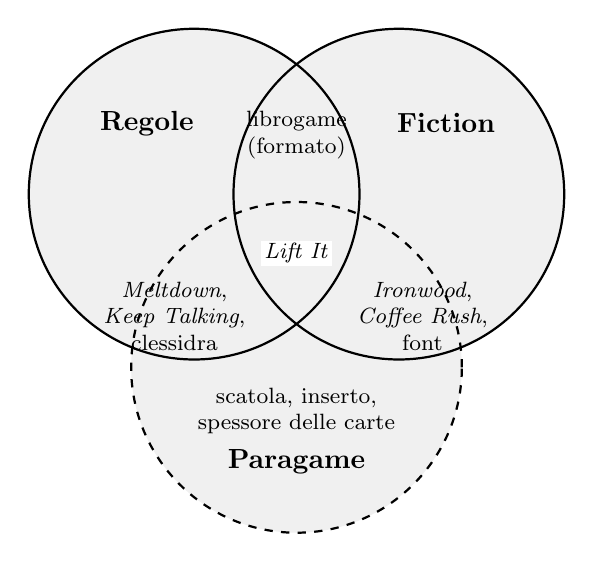
\begin{tikzpicture}[font=\small]
  \fill[gray!12] (0,0) circle (2.1cm);
  \fill[gray!12] (2.6,0) circle (2.1cm);
  \fill[gray!12] (1.3,-2.2) circle (2.1cm);
  \draw[thick] (0,0) circle (2.1cm);
  \draw[thick] (2.6,0) circle (2.1cm);
  \draw[thick, dashed] (1.3,-2.2) circle (2.1cm);
  \node[font=\bfseries] at (-0.6,0.9) {Regole};
  \node[font=\bfseries] at (3.2,0.9) {Fiction};
  \node[font=\bfseries] at (1.3,-3.4) {Paragame};
  \node[font=\footnotesize, align=center] at (1.3,0.75) {librogame\\(formato)};
  \node[font=\footnotesize, align=center] at (-0.25,-1.55)
    {\emph{Meltdown},\\\emph{Keep Talking},\\clessidra};
  \node[font=\footnotesize, align=center] at (2.9,-1.55)
    {\emph{Ironwood},\\\emph{Coffee Rush},\\font};
  \node[font=\footnotesize, align=center, fill=white, inner sep=1pt]
    at (1.3,-0.75) {\emph{Lift It}};
  \node[font=\footnotesize, align=center] at (1.3,-2.75)
    {scatola, inserto,\\spessore delle carte};
\end{tikzpicture}
\caption{Regole, fiction e paragame come tre aree con i bordi sfumati. Il paragame è
ciò che non è né regole né fiction, ma si sovrappone spesso a entrambe. La posizione
degli esempi riprende i commenti di Ruggero durante la lezione: \emph{Lift It} ``è al
centro'', \emph{Ironwood} aiuta soprattutto la fiction, \emph{Meltdown} e \emph{Keep
Talking and Nobody Explodes} soprattutto le meccaniche.}
\label{a10:fig:aree}
\end{figure}

\paragraph{Approfondimento: Genette e le ``soglie'' del testo.} Il termine
\emph{paratesto} viene dal critico francese Gérard Genette, che lo ha sistematizzato in
\emph{Soglie} (\emph{Seuils}, 1987). Per Genette il paratesto è ciò che fa di un testo
un libro e lo presenta al lettore: il titolo, il nome dell'autore, la copertina, le
dediche, le prefazioni, le note, ma anche il formato, la collana, la tipografia. È una
``soglia'' tra l'interno e l'esterno del testo, una zona di transizione che orienta la
lettura. L'idea di applicare lo stesso concetto ai giochi (paragame, paragioco) è
diffusa nei \emph{game studies}, dove il termine \emph{paratext} viene usato anche per
tutto ciò che circonda un gioco (\emph{trailer}, recensioni, guide, comunità). Nella
lezione di Ruggero il senso è più vicino a quello originale di Genette: le
caratteristiche materiali e formali dell'oggetto-gioco.

% ---------------------------------------------------------------------
\section{Le aree del paragame}
\label{a10:sec:aree}

``Su quali aspetti del paragame possiamo lavorare? E qui abbiamo l'ondata di robe.
Andiamo con calma: sono tante zone, ma sono sicuro che le vediamo tutte.'' La
tabella~\ref{a10:tab:aree} le riassume; le sezioni seguenti le vedono una per una.

\begin{table}[htbp]
\centering
\small
\begin{tabular}{@{}p{3.1cm}p{5.4cm}p{4.7cm}@{}}
\toprule
\textbf{Area} & \textbf{Domande da farsi} & \textbf{Esempi della lezione} \\
\midrule
Materialità & di che cosa sono fatti i componenti? Serve un'app? Quanto sono spesse
le carte? Clessidra o timer? & dadi di legno e di plastica; \emph{Lands of Galzyr} su
tablet e telefono; carte \emph{blue core}; \emph{standee} \\
Formato & come sono comunicati regole e testi? Che font, che dimensione, che misura
della carta? & \emph{Bureaucracy} di \emph{Magic}; il \emph{200 Word RPG} \\
Regolamento & quante pagine? Quanti libretti? Video, glossario, \emph{playthrough},
\emph{play aid}? & \emph{Irish Gauge}; \emph{Root}; riassunto delle icone \\
Scatola & dove andrà, nei negozi e a casa? & le vecchie scatole lunghe; la Kallax;
\emph{Dobro} \\
Grafica e illustrazioni & che cosa comunica l'aspetto visivo? Quante icone? &
\emph{Master of Rules}; \emph{Rolling Stock Stars}; \emph{A Feast for Odin} \\
Interfaccia analogica & com'è il \emph{wireframe}? Dove stanno le informazioni quando
il componente è in uso? & la carta di \emph{Magic}; la plancia di \emph{The
Gallerist}; le carte a ventaglio e i mancini \\
Ambiente & dove si gioca? Quanto spazio serve? Che suoni, che vibrazioni? & il tavolo
IKEA; il treno e l'aereo; \emph{Jenga} \\
Audio & serve una colonna sonora? & \emph{Escape: The Curse of the Temple} \\
Contesto & che cosa deve sapere chi gioca sul luogo e sulla cultura del gioco? &
\emph{Jakarta Traffic}; \emph{This War of Mine} \\
Lingua & il gioco dipende dalla lingua? & i giochi di Lacerda; \emph{Race for the
Galaxy}; \emph{Magic} \\
Spazio urbano e ibridi & la città, la stanza, il telefono come parte del gioco &
\emph{Pac-Manhattan}; \emph{Vroom}; \emph{World of Yoho} \\
\bottomrule
\end{tabular}
\caption{Le aree progettabili del paragame presentate a lezione, con le domande che
suggeriscono e gli esempi usati da Ruggero. Inserti e \emph{setup}, discussi alla fine
(sezione~\ref{a10:sec:inserti}), sono un'altra area della stessa famiglia.}
\label{a10:tab:aree}
\end{table}

% ---------------------------------------------------------------------
\section{Materialità}
\label{a10:sec:materialita}

La prima area è la \textbf{materialità}: ``le proprietà fisiche degli elementi di
gioco''. Legno, plastica, metallo. Prendiamo dei dadi classici di legno e dei dadi di
plastica: che cosa cambia? ``Il rimbalzo, il rumore, la sensazione al tatto.'' Sono
aspetti \textbf{cinestetici}, ``che assolutamente impattano''. Ma cambia anche altro,
``perché nel paragame spesso ci sono anche degli \textbf{aspetti culturali}''. In un
Eurogame, in un \emph{German}, si troveranno dadi di legno; in un \emph{American}, in un
\emph{dungeon crawler}, dadi di plastica. (Se n'era parlato, ``vagamente'', nella
lezione sui casi studio, a proposito dei componenti.)

\subsection{Il digitale come materiale}

Anche il \textbf{digitale} fa parte della materialità: se il gioco ha o richiede
un'app, un cellulare, un tablet, ``quello è un aspetto di materialità da considerare''.
Ruggero porta un esempio di un gioco che ha giocato, che la trascrizione chiama ``Lens
of Galsy''\footnote{Con ogni probabilità \emph{Lands of Galzyr} (Snowbright Studio,
2021), gioco d'avventura narrativo con app.}: ``molto carino, ma chiaramente pensato per
un tablet''. L'app ha tanto testo e tante cose a schermo, e sul cellulare, molto più
piccolo, ``non si vede niente''. ``L'app è la stessa, ma in base a dove lo stiamo
giocando, quel gioco può diventare un incubo di accessibilità, o qualcosa invece molto
più comodo da giocare.''

\subsection{Le carte non sono tutte uguali}

Quanto sono spesse le carte? Di che materiale sono? \emph{Blue core}, \emph{black
core}, \emph{white core}? ``Le carte non sono tutte uguali. Vi sembrano uguali perché le
usate da chi gioca, ma da produrre sono diverse.'' Quelle ``che si spaccano al volo'' si
riconoscono subito, perché sono le più economiche: di solito quelle di giochi come
\emph{Uno} o di giochi di carte ``più cheap da produrre'', in cui basta una pieghetta
per rovinare una carta ``forever and ever''. Altri giochi usano il \emph{blue core} o il
\emph{black core}; le carte di \emph{Magic}, per esempio, hanno il \emph{blue core}.

Ruggero semplifica la struttura: di solito una carta da gioco ha \textbf{tre strati},
lo strato con l'immagine sul fronte, quello con l'immagine sul retro, e in mezzo il
materiale che ne determina, tendenzialmente, la \textbf{rigidità}. ``Poi è più
complessa di così'', perché ci possono essere filigrane, texture e altro; ma la parte
centrale dice che cosa succede quando la carta si piega, o quando la si mescola male.

\paragraph{Le carte americane.} Una studentessa chiede delle carte da gioco americane,
``quelle di tela'', come le \emph{Bicycle}, che in Europa si vedono poco: c'è un motivo
per cui sono ``molto più fighe''? Sì: hanno una produzione che include \textbf{materiali
plastici} nella loro texture, che le rende più resistenti e crea un \textbf{attrito}
diverso. Sono carte che ``scivolano molto bene'' (``non ho più italiano, scusatemi''), e
infatti sono usatissime negli spettacoli di prestigiazione, perché si possono manovrare
velocemente, ``per chi le sa maneggiare; io no, di sicuro''. Le carte prodotte in Europa,
invece, hanno di solito un attrito molto più alto, e sono ``non fantastiche'' da usare
in modo ``sgaggio''.

\paragraph{Europa, America, Cina.} Lo stesso vale per i dadi: l'America fa un uso
abbondante di plastica nei giochi perché spesso produce in \textbf{Cina}, mentre
tipografie, stamperie e aziende che producono carte in Europa hanno ``molto poco
accesso'' a quei materiali. ``Quindi spesso siamo più forti nel legno e nella carta che
nella plastica.'' È ``un vaso di Pandora che a voi interessa il giusto'': per i progetti
del corso, quel tipo di finiture ``ve lo sognate, salvo pagare un bordello''. Ci sono
alcune fabbriche che possono fare cose bizzarre, nell'Est Europa e in Repubblica Ceca,
ma la maggior parte di chi produce stampa in Cina, oppure non usa quei materiali.

\paragraph{Miniature e \emph{standee}.} Stesso discorso per le miniature o gli
\textbf{\emph{standee}}, il cartoncino infilato in un piedistallo al posto della
miniatura di plastica. In un \emph{American} è facile trovare la plastica; in un gioco
prodotto e stampato in Europa, ``non trovate delle miniature di plastica'', perché non
c'è praticamente nessuna azienda europea di giochi da tavolo che possa stampare in
Europa la plastica a iniezione usata per le miniature; anche chi produce in Europa giochi
con parti di plastica le fa stampare in Cina. Per questo molti giochi europei degli anni
'90 e 2000, \emph{German} ed Eurogame, ``la plastica proprio la skippano'': se hanno
delle figure, sono \emph{standee}.

\paragraph{Approfondimento: che cosa fa davvero il ``core''.} Nella produzione di carte
da gioco lo strato centrale (\emph{core}) ha due funzioni: dà rigidità e soprattutto
rende la carta \textbf{opaca}, impedendo di vedere il fronte in controluce, cosa
essenziale in qualunque gioco con informazioni nascoste. \emph{Blue core} e
\emph{black core} sono nomi commerciali di cartoncini a più strati con un'anima
colorata scura. Sulle carte americane del tipo \emph{Bicycle}, il cartoncino è in
genere rivestito da una finitura goffrata e laccata (la cosiddetta \emph{air-cushion
finish}) che riduce l'attrito; le carte \emph{interamente} di plastica (PVC o acetato)
esistono, ma sono un prodotto diverso e più costoso.

\subsection{Clessidra o timer?}

``Occhio alla materialità, perché la materialità non va a impattare solo il paragame e
basta.'' Il classico esempio di materialità che impatta anche le \textbf{regole} è la
\textbf{clessidra}. Che differenza c'è tra un timer sul cellulare e una clessidra? Uno
studente risponde: ``la tangibilità''. Sì, e soprattutto quella che si chiama di solito
l'\textbf{informazione discreta}: con il timer si sa con precisione quando mancano un
secondo, due, tre, quattro secondi. Con la clessidra no: si vede chiaramente quando è
finita, ma ha ``quel pizzichino di incertezza che crea una tensione molto precisa che il
timer non ha''. Entrambi creano tensione, adrenalina, frenesia, ma in modo diverso; e
sapere quale dei due serve al proprio gioco ``non è così scontato''
(tabella~\ref{a10:tab:clessidra}).

\begin{table}[htbp]
\centering
\small
\begin{tabular}{@{}p{3cm}p{5cm}p{5cm}@{}}
\toprule
 & \textbf{Timer (cellulare)} & \textbf{Clessidra} \\
\midrule
Informazione & discreta e precisa: si sa quanti secondi mancano & continua e
incerta: si vede la sabbia scendere, ma non si sa con precisione quanto manca \\
Tensione & c'è, ed è ``contata'' & c'è, con ``un pizzichino di incertezza'' in più \\
Fiction & neutra, a meno di suoni scelti apposta & può essere diegetica (vedi il
fiammifero di \emph{Scandal in the Deep}, sezione~\ref{a10:sec:casi}) \\
Domanda da farsi & perché un timer e non una clessidra? & perché una clessidra e non
un timer? \\
\bottomrule
\end{tabular}
\caption{Timer e clessidra come scelta di materialità che incide sulle regole e sulla
tensione di gioco.}
\label{a10:tab:clessidra}
\end{table}

Qui Ruggero fa un annuncio che vale per il resto del corso: ``io ve lo ricordo, ve
l'avevo già accennato, ve lo ripeto: quando vedremo i \emph{pitch}, ma anche i vostri
progetti più avanti, nelle ultime lezioni, \textbf{io vi chiederò tantissimi
perché}''. Perché avete scelto una cosa, perché l'avete fatta, perché l'avete decisa.
``Se avete una clessidra e non un timer, io vi chiederò perché avete una clessidra e non
un timer. Perché avete la plastica, la carta, e così via. Voi dovete dirmi il perché
delle cose che fate.''

% ---------------------------------------------------------------------
\section{Formato}
\label{a10:sec:formato}

Il \textbf{formato} è il modo in cui sono comunicati, per esempio, regole e testi:
frasi o icone? Che font? Quanto è alto, che dimensione ha? E la carta, com'è fatta,
quanto è grande?

\paragraph{\emph{Bureaucracy}.} Il primo esempio è una carta di \emph{Magic} ``volutamente
fatta male'': \emph{Bureaucracy}, da una di quelle serie \emph{easter egg} (umoristiche)
che \emph{Magic} pubblica ogni tanto\footnote{La trascrizione aggiunge un dettaglio
sul simbolo dell'espansione che non è ricostruibile (``ha l'uomo rotto suonate come
simbolo''). \emph{Bureaucracy} appartiene alle espansioni parodiche di \emph{Magic}, le
cosiddette \emph{Un-set}.}. Per il testo è stato scelto un font piccolissimo (``mi
sembra che fosse un corpo 5, o addirittura 6''), per renderlo ``un muro di testo
oppressivo'': tematicamente coerente con il nome della carta.

\paragraph{La misura delle carte di \emph{Magic}.} Qualcuno sa quanto sono grandi le
carte di \emph{Magic}? ``Una dimensione da poker.'' In millimetri sono ``cifre
bizzarre'', perché in realtà la misura è di \textbf{3,5 per 2,5 pollici}\footnote{La
trascrizione riporta cifre storpiate (``88,4 per 69,5''). 3,5 per 2,5 pollici sono circa
88,9 per 63,5 millimetri; la misura nominale indicata di solito per le carte di
\emph{Magic} è 63 per 88 millimetri.}, ``in un sistema stupido americano di
misurazione'' (``ormai l'ho detto, è troppo tardi''). E in quella dimensione non c'è
tutto lo spazio che si vuole, perché una parte è dedicata all'\textbf{illustrazione}:
lo spazio per il testo, con il font e la dimensione scelti, è ancora più ridotto.
Questo non impatta solo il formato, ma anche le \textbf{regole}: ``una regola complessa
sarà difficile da scrivere in quello spazio'', e quindi il formato costringe a scegliere
regole che ci stiano dentro.

\paragraph{Il \emph{200 Word RPG}.} Un caso estremo: il \emph{200 Word RPG}, una sfida
in cui si scrivono giochi di ruolo completi in \textbf{200 parole}. Il paragame è il
formato stesso delle 200 parole: ``ditemi voi se non vi impatta le regole, quel
formato''.

``Non prendete questa cosa qua come del contorno, come una cosa che è un di più.
Questa roba qui vi va a impattare come voi create i giochi, e se lo sapete, potete
lavorarci attorno.''

% ---------------------------------------------------------------------
\section{Regolamento}
\label{a10:sec:regolamento}

Il \textbf{regolamento} è un'area a sé. Quante pagine ha? Una o quaranta? Che cosa
cambia? ``Se io vi dico: venite, c'è un party game, e tiro fuori un manuale da 60
pagine, che cosa succede?'' Succede che nessuno lo gioca.

\paragraph{\emph{Irish Gauge}: un caso positivo.} All'opposto, un caso ``incredibile'':
\emph{Irish Gauge}\footnote{La trascrizione dice ``Irish Gouge'' e attribuisce il gioco a
``Amable Holland'', più avanti ``Anne Blowland''. È \emph{Irish Gauge}, gioco
ferroviario di Amabel Holland.}, un gioco economico ferroviario ``bellissimo'', di circa
un'ora di partita, in cui si comprano azioni e si costruiscono ferrovie, con una
complessità significativa sul tavolo, ``un gioco comunque bello intenso''. E il
regolamento è \textbf{un singolo foglio di carta} ``che lascia zero dubbi dopo che lo si
è letto''. ``Bellissimo, irraggiungibile forse.'' È una sorpresa positiva; il caso
contrario (il party game da 60 pagine) è una sorpresa negativa che uccide il gioco.

\paragraph{QR code e video.} Chi gioca spesso avrà notato che sempre più regolamenti
hanno un \textbf{QR code} o un link a un video in cui le regole vengono spiegate.
Perché? ``Non sappiamo più leggere'' è ``la versione più nichilista''. La risposta ``più
banale e meno nichilista'' è che \textbf{le persone imparano in modi diversi}: un
regolamento scritto in un certo modo può andare benone per una persona ed essere un
disastro per un'altra.

\paragraph{Più libretti per lo stesso gioco.} Alcuni giochi hanno più di un libretto di
regole. \emph{Root}, per esempio, ha la \textbf{guida rapida} (il \emph{learn to play}),
scritta come un regolamento da leggere al tavolo, e la \textbf{Legge di Root}, scritta
come un \textbf{manuale tecnico}: paragrafi 1.1.1, 1.1.2, 1.1.3, 1.2.1 e così via, con
glossario. ``Il gioco è lo stesso. Lo si impara a giocare in entrambi i modi, ma parlano
a due persone completamente diverse.''

\paragraph{I costi.} Ogni scelta ha un costo. Un regolamento in più costa la
produzione di un regolamento in più, \textbf{a ogni copia} stampata. Il video è un costo
diverso: lo si paga una volta, all'inizio, lo si mette online ``e quel video lì è lì''.
``Se tu stampi 100 copie o ne stampi 10.000, il video non ti costa di più. Il
regolamento sì.''

\paragraph{Glossario, \emph{playthrough}, \emph{play aid}.} Altre domande: c'è un
\textbf{glossario}? Un \emph{playthrough}? Un \emph{play aid}? E le icone, dove sono
riassunte? Dove si trova di solito il riassunto delle icone? Due risposte, ``entrambe
vere''. Tancredi: \textbf{nell'ultima pagina del regolamento}, usata spesso proprio per
questo, perché si può tenere il regolamento girato sul tavolo e avere il riassunto
davanti. Tiziana: in un \textbf{\emph{play aid}}, un cartoncino, magari uno a persona,
con il riassunto delle icone. Quando l'uno e quando l'altro? Dipende da \textbf{quante
icone} ha il gioco. In \emph{Race for the Galaxy} un riassunto a testa non esiste,
``perché il riassunto delle icone di \emph{Race for the Galaxy} è così'' (e Ruggero
mostra quanto è lungo). In giochi con cinque, sei, una decina di icone è facile avere
una carta personale che le riassume, magari con il \textbf{flusso del turno} sul retro.

\paragraph{Il \emph{playthrough} e l'\emph{actual play}.} Più avanti, su richiesta di
uno studente (``Ruggero, non so se l'hai detto: il \emph{playthrough}?''), Ruggero torna
sul punto. Il \textbf{\emph{playthrough}} è \textbf{una giocata descritta}. Molti giochi
lo fanno spezzandolo in esempi: i classici esempi in cui ``Tizio e Caio fanno A, B, C,
poi Tizio fa B e Caio piange perché ha perso la partita''. Questi esempi non sono solo
un'applicazione delle regole: sono una descrizione di \textbf{che cosa fanno le persone
al tavolo}. Alcuni giochi, soprattutto di ruolo, includono il cosiddetto \textbf{\emph{actual
play}}: un'intera partita descritta, alternando le parti di \emph{roleplay} e quelle
meccaniche (``Tizio tira e fa 18, quindi apre questa cosa; poi Caio dice questa cosa con
il suo personaggio''). Dove si trovano\footnote{La trascrizione attribuisce la domanda a
qualcuno che si rivolge a ``Pietro''; con ogni probabilità è un errore di trascrizione
per ``Ruggero''.}? Sono ``comunissimi nei giochi di ruolo'': molti giochi di ruolo
contemporanei hanno esempi di \emph{actual play}, di solito in fondo al manuale. Gli
esempi sparsi nei regolamenti sono ``un'estrazione del \emph{playthrough}'', scritti con
la stessa idea; il \emph{playthrough} vero e proprio è l'esempio di partita completa. Nei
giochi da tavolo più commerciali è raro, ``perché le pagine dei regolamenti costano'', e
una partita completa prende molto spazio. Rientra quindi soprattutto nei giochi di
ruolo, che hanno già manuali da cento pagine e passa e non hanno il problema di stare
sotto le 16 pagine, ``perché sennò la gente si spaventa'' davanti a un regolamento da
20.

% ---------------------------------------------------------------------
\section{La scatola}
\label{a10:sec:scatola}

Nel formato rientra anche la \textbf{scatola}. Ruggero è convinto di averne già parlato
(``non abbiamo mai parlato delle scatole? Secondo me no'') e la affronta con una
domanda: come erano fatte le scatole del vecchio \emph{Risiko!} o del vecchio
\emph{Monopoly}? ``Basse e lunghe.'' Perché? ``Ci stava il tabellone''; ``si impilavano''.
La domanda, precisa Ruggero, non è che cosa c'era dentro, ma \textbf{dove doveva andare}
la scatola: nei negozi di giocattoli e, a casa, dove venivano messi i giochi trenta,
quarant'anni fa? Non nella libreria: \textbf{negli armadi}. ``Non era una questione
estetica'': l'armadio è stretto e lungo, e la scatola doveva entrare lì.

E oggi, dove vanno messi? In libreria. Quale libreria? La \textbf{Kallax}\footnote{La
trascrizione dice ``Callax'' e, a tratti, ``Galaxy''.} dell'IKEA, ``la libreria più
venduta del mondo''. Com'è fatta? ``\textbf{A cubi}.'' La scatola del vecchio
\emph{Monopoly} lì dentro non entra (``puoi metterla in cima, certo''). Ma se oggi un
editore vuole che il suo gioco entri ``nella libreria più venduta del mondo'', il gioco
deve entrare in un cubo. ``È tutto qui. \textbf{Una scelta dell'IKEA ha deciso che le
nostre scatole ora sono quadrate}.'' L'IKEA non ha convinto gli editori di niente: ``è
una roba che viene naturale, perché tutta l'umanità è intrecciata. Le decisioni che
prende qualcuno vanno a impattare qualcun altro''. Chi vuole che il proprio gioco sia in
vista in libreria deve fare i conti con il cubo.

Ruggero si concede qui una raccomandazione generale: ``se c'è una cosa che voglio che vi
portiate via da questo corso, una cosa'' (``poi, se fate anche giochi dopo, belli,
benissimo''), ``la cosa migliore per me, perché sono contento, ho fatto il mio lavoro,
posso morire in pace'', è questa: \textbf{ragionate quando fate le cose}. ``Potete
ragionare sulle cose quanto volete. Più ci ragionate, più avete aree operative su cui
fare le cose.''

\paragraph{Approfondimento: il ``formato Kallax''.} Il vano interno di una Kallax misura
circa 33 per 33 centimetri, per una profondità di poco inferiore ai 39. Non a caso un
gran numero di giochi da tavolo contemporanei di formato ``standard'' ha una scatola
quadrata di circa 30 centimetri di lato: è il formato che sta in un vano in piedi o
coricato, e che si impila bene. Molti editori lo indicano ormai esplicitamente tra i
vincoli di progettazione della scatola, insieme al peso e ai costi di spedizione.

% ---------------------------------------------------------------------
\section{Grafica e illustrazioni}
\label{a10:sec:grafica}

``\textbf{Graphic design e illustrazioni sono due cose diverse}. Non confondete le
cose.'' Le \textbf{illustrazioni} sono tendenzialmente l'\emph{art}: le immagini,
gli sfondi, i personaggi, i luoghi, la parte di \emph{world building}. Il
\textbf{graphic design} sono le icone, la UX. ``Non fate fare queste due cose alla
stessa persona, sennò di solito viene una porcheria.''

\subsection{Due edizioni, due destini}

Sulla slide ci sono due scatole: una con un omino che tiene sopra di sé delle forme, e
una con un'auto sotto un cielo stellato, una notte al neon. ``Sono lo stesso gioco'':
\emph{Master of Rules}\footnote{Il titolo è quello della trascrizione e non è stato
possibile verificarlo.}, ``un gioco bellissimo'', che nella sua edizione americana è
uscito con la prima scatola. ``Vi sorprenderà sapere che in America non è andato per
niente, nonostante sia un gioco incredibile. Qualcuno ha un'idea del perché?'' Le
risposte sono impietose: ``fa schifo'', ``sembra quelli che trovi in edicola''. E
dentro, dice Ruggero, ``è ancora più brutto''.

Uno studente lo provoca: ``io ho dei giochi che hanno copertine orrende da 100 euro'':
gli \textbf{Splotter}\footnote{Splotter Spellen, editore olandese noto per giochi
molto pesanti e per una grafica spartana.}. Ruggero non lo nega, ma ribalta la
domanda: la grafica degli Splotter ``è comprensibile perché la fanno così, ovvero perché
non gliene frega niente''; ma ``sarebbero giochi peggiori con una grafica migliore?'' ``La
risposta, nel tuo cuore, la sai: no.'' Le immagini danno un'esperienza, un \emph{look
and feel}.

Tiziana porta un caso concreto: un amico ha comprato \emph{Darwin's Journey}\footnote{
La trascrizione dice ``Darvis Journey''.}, ``un gioco che secondo me è bellissimo'', e
l'ha rivenduto, perché l'impatto grafico per lui è stato terribile: ``colori scuri sul
marrone''. ``Non riusciva a vederlo.''

Ruggero avrebbe potuto fare ``mille altri esempi'' di giochi usciti in due edizioni con
grafiche diverse, ``una che va a picco e non la vedete più, e l'altra che invece diventa
roba di culto''. Perché la grafica ha un impatto ``non solamente in termini di
leggibilità, ma anche di \emph{vibes}''. Lui, personalmente, non ci fa caso: ``io mi
gioco anche \emph{Rolling Stock Stars}'', che ``sembra fatto da marito e moglie su
Excel''. Ma altre persone vedono quella grafica e dicono ``non giochiamo a \emph{Rolling
Stock Stars}''. E finisce che ``il piccolo Ruggero'' lo gioca ``una volta ogni cinque
anni, perché nessuno vuole giocarci''. La conclusione: ``un gioco può beneficiare
dall'essere \textbf{non visivamente ostile} alle persone che lo vogliono giocare''.
Un altro studente aggiunge, a proposito di grafiche difficili, \emph{Terraforming
Mars} (``la carta con il cane''), e Ruggero si arrende: ``volete farmi stare male
oggi''.

\subsection{Il font, e quante icone}

Anche il \textbf{font} rientra nella grafica, non solo nel formato: il font del titolo,
il font dei contenuti. Ruggero cita un gioco che ha venduto ``proprio per il font che
aveva'', e promette di mostrarlo dopo, perché ``ci vuole del tempo per elaborare''
(lo farà nella discussione finale: è \emph{Al Rashid}, sezione~\ref{a10:sec:alrashid}).

Ultimo punto della grafica: \textbf{quante e quali icone} avete? Sulla slide c'è \emph{A
Feast for Odin}\footnote{La trascrizione dice ``Fist for Odin''. \emph{A Feast for
Odin} (Uwe Rosenberg, 2016).}: ``quel gioco lì ha 50 azioni diverse. Non devo dirvi
altro''. Ragionate sulle icone che avete.

\paragraph{L'intervento di Tiziana.} Tiziana porta un esempio di segno opposto: ha
giocato di recente a un gioco che la trascrizione chiama ``MNFR''\footnote{Il titolo
non è ricostruibile dalla trascrizione.}, abbastanza complesso, con varie tipologie di
azioni e una serie di cose che si succedono; ma le icone ``sono sempre quelle'', in
numero limitato, e una volta capite ``te le ritrovi in tutte le salse, nelle varie parti
e sezioni del gioco''. ``E questo aiuta molto.'' Ruggero concorda e cita di nuovo
\emph{The Gallerist} (``bellissimo, un capolavoro''): sono giochi in cui, se si fa un
buon lavoro sulle icone, il gioco ``non ti chiederà mai di andare a leggere il
regolamento durante la partita''. Lui ha giocato di recente un Eurogame di designer
giapponesi\footnote{La trascrizione dice ``Elder Tide degli stessi di Gisoji''; titolo
e autori non sono ricostruibili con sicurezza.}, con un \emph{setting} un po' fantasy, in
cui si costruiscono edifici su un'isola e ci si muove di porto in porto per vendere
risorse: ``ha tante icone, ma dopo i primi cinque minuti, per tutte le altre due ore
della partita, non abbiamo guardato il regolamento una singola volta, perché è tutto
chiaro, tutto immediato''. Si torna ai pilastri: immediatezza, efficienza,
memorabilità.

% ---------------------------------------------------------------------
\section{Interfaccia analogica}
\label{a10:sec:interfaccia}

La voce successiva è l'\textbf{interfaccia analogica}: ``si parla di
\emph{wireframing}, di solito''. È la struttura nuda della carta, quelle linee che, in
stampa, ``verranno abbellite da frame, cornici''. Ma il \emph{wireframe} è quello. ``Se
vi chiedo di disegnarmi a occhi chiusi su un foglio una carta di \emph{Magic}, voi sapete
come disegnarmela'': divisa a metà, al centro un rettangolino molto sottile, un
rettangolo più grosso in alto, uno più grosso in basso. ``Quella parte lì è una parte su
cui potete ragionare.''

\subsection{La scatola in piedi: \emph{Dobro}}

Anche la grafica della scatola è interfaccia. ``Se io prendo la scatola e la metto in
verticale, posso leggere il titolo?'' C'è una ``diatriba'' che Ruggero non apre
(``siete ancora persone sane di mente, non voglio rovinarvi la vita''): i giochi da
tavolo si mettono in libreria in verticale o in orizzontale? Lui fa un mix, ma molte
persone li mettono in verticale, e molte scatole non hanno il nome del gioco su tutti i
lati: alcune lo hanno solo per il lungo, e in verticale il nome è storto. L'esempio
positivo è \emph{Dobro}, di cui il suo gruppo ha rifatto la scatola per l'edizione
italiana: un lato lungo con il nome in orizzontale, il lato opposto con il nome in
verticale, e lo stesso sui due lati corti. ``Non importa come la mettete: un modo per
trovarla con il nome che si vede da fuori lo trovate sicuramente.'' Mentre ``ho delle
scatole in cui non si vede il nome, perché purtroppo non l'hanno messo su tutti i
lati''. Quindi: \textbf{la grafica della scatola non va lasciata al caso}, ``perché è
funzionale''. (``Mi sto arrabbiando, si vede, perché questa cosa mi fomenta.
Purtroppo per voi.'')

\subsection{Le opere sulla plancia di \emph{The Gallerist}}

Una studentessa chiede di chiarire: l'interfaccia analogica è il discorso della scatola
e della visibilità, o altro? Ruggero torna al \emph{wireframe}, ``cioè a come sono fatte
le carte'', e porta l'esempio di \emph{The Gallerist}: si acquistano opere d'arte da
esporre nella propria galleria, e la \textbf{plancia} personale raffigura la galleria.
Le tre tessere delle opere esposte si sovrappongono perfettamente ai \textbf{muri
disegnati sulla plancia}, ``andando letteralmente a mettere le opere in vista nella
nostra galleria''. Non è casuale: hanno pensato la grafica in modo che aiutasse a capire
che cos'è quel componente, e in modo che fosse anche soddisfacente. Di nuovo:
soddisfazione, efficienza, memorabilità, immediatezza.

\subsection{Dove stanno le informazioni quando le carte sono in mano}

Un altro aspetto dell'interfaccia è \textbf{dove si piazzano le informazioni}. Con le
carte da poker in mano, dove sono le icone? \textbf{In alto a sinistra}: quando le carte
sono aperte a ventaglio, ciascuna copre buona parte di quella precedente, e l'angolo in
alto a sinistra è ``la cosa più visibile'' (figura~\ref{a10:fig:ventaglio}).

Tancredi apre una parentesi sui \textbf{mancini}: ``io da mancino, tutte le volte che
apro le carte da poker, non vedo assolutamente niente''. Ruggero conferma (``ho degli
amici mancini, e se avete un gioco che non pensa ai mancini lo sapete al volo, perché
ve lo dicono''), e lo riconduce all'\textbf{accessibilità}: i mancini tengono in mano le
carte come tutti, ``è solo che per natura il ventaglio lo fanno nell'altro verso''. Molti
giochi per questo \textbf{duplicano} il seme della carta, mettendolo anche in alto a
destra. In alcuni giochi è più complicato: quando l'angolo in alto a sinistra ospita
icone meccaniche, come il costo, come in \emph{Race for the Galaxy} (``è il problema
minore di questa carta, mi sento di dire''), duplicare vuol dire affollare ancora di più
una carta già piena. ``Volete davvero duplicare le informazioni di questa carta
dall'altro lato? Io non lo farei.'' Non sempre si può; ma ``è assolutamente una
considerazione da fare''.

\begin{figure}[htbp]
\centering
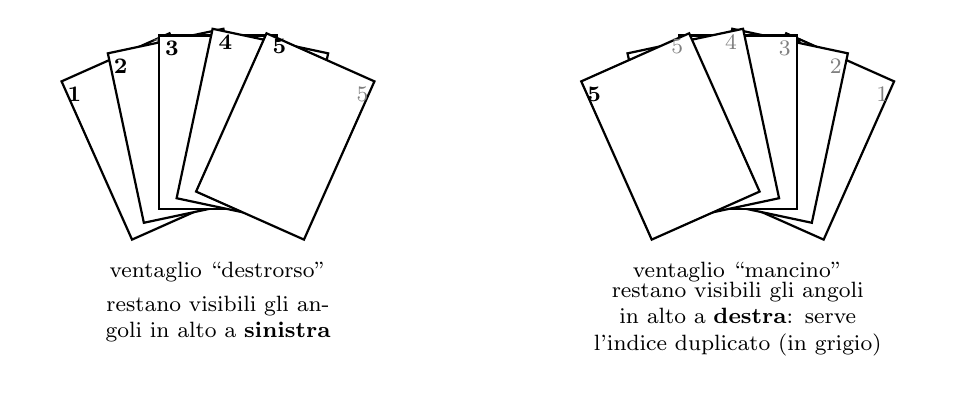
\begin{tikzpicture}[font=\footnotesize]
  % mano destrorsa: ventaglio verso destra
  \begin{scope}[shift={(0,0)}]
    \foreach \a/\i in {24/1, 12/2, 0/3, -12/4, -24/5}{
      \begin{scope}[rotate around={\a:(0,-2.6)}]
        \draw[thick, fill=white] (-0.75,-1.6) rectangle (0.75,0.6);
        \node[anchor=north west, inner sep=2pt] at (-0.75,0.6) {\textbf{\i}};
        \node[anchor=north east, inner sep=2pt, text=gray] at (0.75,0.6) {\i};
      \end{scope}
    }
    \node at (0,-2.4) {ventaglio ``destrorso''};
    \node[text width=4.6cm, align=center] at (0,-3.0)
      {restano visibili gli angoli in alto a \textbf{sinistra}};
  \end{scope}
  % mano mancina: ventaglio nell'altro verso
  \begin{scope}[shift={(6.6,0)}]
    \foreach \a/\i in {-24/1, -12/2, 0/3, 12/4, 24/5}{
      \begin{scope}[rotate around={\a:(0,-2.6)}]
        \draw[thick, fill=white] (-0.75,-1.6) rectangle (0.75,0.6);
        \node[anchor=north west, inner sep=2pt] at (-0.75,0.6) {\textbf{\i}};
        \node[anchor=north east, inner sep=2pt, text=gray] at (0.75,0.6) {\i};
      \end{scope}
    }
    \node at (0,-2.4) {ventaglio ``mancino''};
    \node[text width=4.6cm, align=center] at (0,-3.0)
      {restano visibili gli angoli in alto a \textbf{destra}: serve l'indice
      duplicato (in grigio)};
  \end{scope}
\end{tikzpicture}
\caption{Le carte a ventaglio. L'informazione più importante va nell'angolo che resta
scoperto; chi apre il ventaglio nell'altro verso, come molti mancini, vede l'angolo
opposto, e per questo molti giochi duplicano il seme o l'indice in alto a destra.
Schema illustrativo: l'ordine con cui le carte si sovrappongono dipende da come le si
apre.}
\label{a10:fig:ventaglio}
\end{figure}

Ruggero annuncia che su grafica e formato c'è ``un'altra cosa'', da riprendere dopo (lo
farà con gli inserti, sezione~\ref{a10:sec:inserti}).

% ---------------------------------------------------------------------
\section{Ambiente}
\label{a10:sec:ambiente}

\textbf{Dove} giocheranno le persone al vostro gioco? Su un tavolo, a letto, per terra,
in piedi? E \textbf{quanto spazio} prende il gioco? Qualcuno sa quanto spazio, al
massimo, deve prendere un gioco da tavolo \emph{family} per quattro persone? ``La sapete
nel vostro cuore, la risposta.'' Gianmarco: ``\textbf{il tavolo IKEA}''. ``Bravissimo,
Gianmarco, è sempre quello.'' Il tavolo IKEA più venduto: cercate quanti centimetri
misura. ``Se il vostro gioco non entra in quel tavolo, avete un grosso problema.''

E se è un \textbf{party game}? Allora deve stare nel \textbf{tavolino da caffè}
dell'IKEA, più piccolo, quello da divano, ``per un altro tipo di ambiente''. Se è un
gioco \emph{pocket}, portatile, deve stare nei tavolini da caffè, in quelli del
\textbf{treno}, in quelli dell'\textbf{aereo}. ``Quanto spazio prende il vostro gioco
apparecchiato non è casuale. Non lasciate al caso quella roba'', altrimenti succede,
come è capitato di vedere a Ruggero, di avere ``giochi in solitaria che prendono un
tavolo per sei persone''.

Il mezzo di trasporto ha poi un altro problema: il treno e l'aereo \textbf{si muovono}.
Il gioco può starci come spazio, ma i componenti? Uno studente ricorda le
\textbf{versioni magnetiche} di scacchi e dama, e una versione mini di \emph{Azul} con
le tessere che si incastrano. E Ruggero aggiunge: \emph{Jenga} ci sta, come spazio, nel
tavolino di un aereo. Perché nessuno ci gioca in aereo? ``Per le vibrazioni dovute al
movimento.'' Appunto: ``l'ambiente non è solo spazio. L'ambiente è anche suoni, è anche
vibrazioni, è un sacco di altre cose''.

\paragraph{Approfondimento: misurare il tavolo.} Le misure dei tavoli più diffusi
nelle case cambiano da modello a modello, ma un tavolo da cucina per quattro persone ha
spesso un piano tra gli 80 per 80 e i 120 per 75 centimetri, e un tavolino da caffè è
molto più piccolo (spesso intorno ai 90 per 55 centimetri). Il consiglio di Ruggero va
preso alla lettera: misurare il piano reale di riferimento e fare un \emph{mock-up} del
gioco apparecchiato a grandezza naturale, lasciando spazio per le mani, i bicchieri, le
plance personali e i mazzi degli scarti. È uno dei test più economici che si possano
fare con un prototipo.

% ---------------------------------------------------------------------
\section{Audio}
\label{a10:sec:audio}

Altra area progettabile: l'\textbf{audio}. Serve la musica nel vostro gioco? Alcuni
giochi usano una \textbf{colonna sonora} per dare il tempo. L'esempio è \emph{Escape:
The Curse of the Temple}\footnote{La trascrizione inciampa più volte sul titolo, e
Ruggero stesso si corregge (``scusatemi, perché in tedesco\dots''). Il gioco è
\emph{Escape: The Curse of the Temple} (Kristian Amundsen \O{}stby, Queen Games, 2012).}: un
gioco in tempo reale in cui bisogna uscire dal tempio entro la durata della colonna
sonora, ``sennò siete fritti''. E a intervalli la colonna sonora fa sentire dei
\textbf{colpi di gong} che attivano eventi meccanici nel gioco. Quindi la colonna
sonora non è ``solamente un timer, una grossa clessidra'': è un \textbf{elemento
meccanico} che, con l'audio, fa altre cose. E fa anche \textbf{fiction}: dà elementi di
\emph{world building}, certe \emph{vibes}. ``È chiaro che \emph{Escape} è molto Indiana
Jones: non avete una colonna sonora techno IDM a palla.''

% ---------------------------------------------------------------------
\section{Contesto}
\label{a10:sec:contesto}

``Al \textbf{contesto} non ci pensa quasi mai nessuno, ma è molto importante'', perché
informa il gioco, ``non solo in termini di \emph{world building}, ma anche in termini di
che cosa vuole che voi facciate''.

\paragraph{\emph{Jakarta Traffic}.} \emph{Jakarta Traffic}\footnote{Titolo come nella
trascrizione.} è un gioco sul traffico di Giacarta, ``che è molto ostile'': si naviga il
traffico per fare delle consegne, e molti elementi del gioco sono \textbf{culturali}.
Spiegare le meccaniche a chi non sa come è fatta Giacarta, culturalmente, rende il gioco
molto più complesso di quanto dovrebbe essere. Qui, secondo Ruggero, hanno fatto un
buon lavoro: il manuale aiuta a capire il contesto, e hanno perfino creato una colonna
sonora usando il traffico di Giacarta come \emph{sample}, per creare un certo
\emph{mood}.

\paragraph{\emph{This War of Mine}.} Ma il contesto non è solo \emph{setting}: può
anche \textbf{informare le scelte}. Qualcuno conosce il gioco da tavolo di \emph{This War
of Mine}\footnote{La trascrizione dice ``Diceworld Mine''.}? Qual è il suo contesto?
``È una guerra, ma non mi ricordo se è una guerra vera.'' ``È a metà'': non è scritto
apertamente, ma è palesemente l'\textbf{assedio di Sarajevo}. E soprattutto, non si
giocano militari: si giocano \textbf{civili}. Se ci si approccia al gioco ``con tutto il
bagaglio culturale dei giochi di guerra'', ci si aspettano cose che il gioco non può
dare, perché ``non è un gioco di soldati in guerra: è un gioco in cui c'è la guerra, ma
non è un gioco di guerra''. Queste cose si risolvono con un mix: in parte con testo,
\emph{flavor} e \emph{world building}, in parte con il paragame, con i materiali.

% ---------------------------------------------------------------------
\section{Lingua}
\label{a10:sec:lingua}

Anche la \textbf{lingua} è un componente. Alcuni giochi sono \textbf{indipendenti dalla
lingua}: in un gioco di Lacerda\footnote{Vital Lacerda, autore portoghese di Eurogame
pesanti, tra cui \emph{The Gallerist}.}, o nella maggior parte dei \emph{German}, sulle
carte non c'è testo, ``alla buon'icona''. Lo stesso \emph{Race for the Galaxy}, lasciando
stare il nome e l'effetto ricopiato sotto, si può giocare anche senza leggere l'inglese:
``mi basta sapere che cosa fanno quelle icone''. Così \emph{The Gallerist}, o \emph{Master
of Rules}. Altri giochi no: \emph{Magic} è molto difficile da giocare se le carte non sono
nella propria lingua.

% ---------------------------------------------------------------------
\section{La città, la stanza, il telefono}
\label{a10:sec:pervasivo}

``In quali altri modi posso impattare l'esperienza di chi gioca senza passare per le
regole e per la fiction?'' Sulla slide c'è un'immagine di
\textbf{\emph{Pac-Manhattan}}\footnote{La trascrizione dice ``Pac-Man Hatton''.
\emph{Pac-Manhattan} (2004) è un gioco urbano nato alla New York University, in cui
persone vere interpretavano Pac-Man e i fantasmi nelle strade di Manhattan.}: la città,
gli aspetti \textbf{pervasivi urbani} sono anch'essi paragame.

\paragraph{La stanza come pista.} Un altro esempio è un gioco di corsa cooperativo che
la trascrizione chiama ``Vroom''\footnote{Il titolo non è stato possibile verificarlo.}:
usa il \textbf{tavolo} come spazio di gioco e chiede di prendere degli \textbf{oggetti
della propria stanza} e metterli sul tavolo come ostacoli, ``fisicamente, proprio''.

\paragraph{\emph{World of Yoho}.} Infine \emph{World of Yoho}\footnote{La trascrizione
dice ``World of Yacht'', ``World of YOHO'', ``Word of Yoko''.}, un gioco di pirati che
chiede di usare il \textbf{cellulare} su un tabellone gigantesco. Il telefono è la
propria \textbf{nave}: quando lo si sposta, sullo schermo si muove la mappa, e le parti
di quella casella di mare diventano interagibili in digitale. ``Si poteva fare senza
cellulare? Sì, con un libro degli eventi gigantesco, una seccatura infinita. Mentre così
è una cosa immediata, che si spiega in tre minuti.'' Uno studente chiede se si giochi su
un tabellone normale: sì, il gioco arriva in scatola con il suo tabellone, che si mette
sul tavolo, e chiede semplicemente di usare il telefono come nave per tutta la partita.
Ogni persona usa il proprio telefono; e nelle battaglie navali ``vedi i proiettili che
vengono sparati da una nave, che vanno sul bordo del telefono ed entrano nell'altro.
Pazzi completi. Bellissimo''.

\medskip
Prima dei casi studio, una seconda pausa: ``sono le 57'', e Ruggero dà otto minuti
``per il numero tondo'': si riprende alle 19:05.

% ---------------------------------------------------------------------
\section{Casi studio}
\label{a10:sec:casi}

``Andiamo avanti nell'ultima parte'': i \textbf{casi studio}, per vedere ``come
applichiamo le cose che abbiamo appena visto a giochi particolari''. Ce ne sarebbero
``a tonnellate''; Ruggero ne ha scelti un gruppo ``che va da giochi più regolari a cose
più \emph{deranged}, come spesso succede'', e per ciascuno dovrebbe essere chiaro perché
è stato scelto. La tabella~\ref{a10:tab:casi} li riassume.

\begin{table}[htbp]
\centering
\small
\begin{tabular}{@{}p{3.3cm}p{5.3cm}p{4.6cm}@{}}
\toprule
\textbf{Gioco} & \textbf{Elemento di paragame} & \textbf{Che cosa tocca} \\
\midrule
\emph{Cuba Libre} & due regolamenti, due diagrammi di flusso per i bot, quattro
brochure di fazione & regole, accessibilità di un gioco pesante \\
\emph{193 Days} & solo un mazzo di carte, niente regolamento & si impara giocando \\
gioco ``a metropolitana'' & creazione del personaggio piegata come una mappa turistica
& fiction, \emph{world building} \\
\emph{Shenzhen I/O} & un manuale fisico da stampare, il faldone della collector's &
meccaniche (le schede tecniche), fiction, ``feeling'' \\
pinball in scatola & dadi da schicchera su una ``scalinata'' con i flipper & meccaniche \\
\emph{Lift It} & la gru da mettersi in testa & ``al centro'' di regole, fiction e
paragame \\
\emph{Coffee Rush} & tazzine di plastica e ingredienti a forma di ingrediente & fiction,
\emph{vibes} \\
\emph{Ironwood} & una fazione tutta di legno, una tutta di metallo & fiction,
riconoscibilità, \emph{vibes} delle fazioni \\
\emph{Nyctophobia} & occhiali oscuranti per chi scappa & meccaniche, accessibilità,
fiction \\
\emph{Keep Talking and Nobody Explodes} & visore VR da una parte, manuale di carta
dall'altra & meccaniche, comunicazione \\
\emph{City of Six Moons} & nessun regolamento: un artefatto ``alieno'' & il gioco stesso
è dedurre le regole \\
\emph{Scandal in the Deep} & un fiammifero acceso come torcia & tempo reale, fiction
diegetica \\
\emph{Metal} & componenti di metalli diversi & meccaniche di destrezza (peso, massa) \\
\emph{Meltdown} & tessere di ghiaccio che si sciolgono & tema e meccaniche, inseparabili
\\
\bottomrule
\end{tabular}
\caption{I casi studio della lezione, in ordine di presentazione, con l'elemento di
paragame che li rende interessanti e l'area con cui si intreccia.}
\label{a10:tab:casi}
\end{table}

\subsection{\emph{Cuba Libre}: sei brochure}

Si parte da un gioco che Ruggero ama: \textbf{\emph{Cuba Libre}} della GMT\footnote{
\emph{Cuba Libre} (Jeff Grossman e Volko Ruhnke, GMT Games, 2013), secondo titolo della
serie COIN (\emph{COunter-INsurgency}).}, uno strategico per quattro persone, da tre o
quattro ore, sulla rivoluzione cubana. Ha tanto materiale cartaceo, inclusi dei
\textbf{diagrammi di flusso}, ``che è la cosa che tendenzialmente può intimorire le
persone''.

In alto, \textbf{due manuali}: \emph{Playbook} e \emph{Rules of Play}. Perché due?
Nessuno ha giocato \emph{Cuba Libre}, ma la classe sa già rispondere: ``forse uno ha più
le regole, l'altro lo sviluppo del gioco''. Esatto. Il \emph{Playbook} accompagna la
partita dal \emph{setup} al turno di gioco, ``scritto come un manuale di gioco da
tavolo''; le \emph{Rules of Play} sono il manuale tecnico visto con \emph{Root}: un
manuale ``con font di corpo 6-7, diviso in paragrafi, con il glossario tecnico alla
fine'', in cui, con un dubbio sul combattimento, si va alla sezione del combattimento e
si è sicuri di trovare il sottoparagrafo che interessa.

Sotto ci sono \textbf{sei ``foglioni''}: A4, ma fronte e retro e piegati a brochure,
``come se avessimo quattro facciate''. Che cosa sono? I due a destra sono
\textbf{diagrammi di flusso}, uguali, con la scritta \emph{Non-Player}: servono quando si
gioca in \textbf{solitario}, o quando si vuole riempire una delle quattro fazioni. È un
gioco a quattro fazioni asimmetriche che ha senso giocare con tutte e quattro: ``ma se
siamo in tre, o in due, che cosa facciamo? Non giochiamo a \emph{Cuba Libre}?'' I
diagrammi simulano nel dettaglio il comportamento di questi \textbf{bot}, ``un'intelligenza
artificiale analogica'', ``nel senso vecchio del termine, non generativa: macchine a
stati''. E il testo scritto è notoriamente un mezzo \textbf{lineare}, che si applica poco
alle macchine a stati; i diagrammi di flusso risolvono questo problema. Già dalla scelta
dello strumento si capisce lo scopo: rendere ``il più veloce e scorrevole possibile la
gestione di automatismi'' delle fazioni giocate dal gioco, ``senza farle troppo
stupide''.

Gli altri quattro sono \textbf{brochure uguali}, fronte e retro: quattro facciate, una per
\textbf{ogni fazione}. A che cosa servono, e perché tutti ne hanno una? Una studentessa:
riassumono le regole specifiche e asimmetriche di ogni fazione, ``e devo sapere che cosa
possono fare gli altri perché possono influire sul mio gioco''. Esatto: in uno
strategico di \emph{counterinsurgency} (``si fanno imboscate, ci si ammazza, ci si
rapisce'') bisogna sapere che cosa può fare l'avversario per impedirgli di fare ``quelle
cose brutte che vuole farmi''. E per farlo bisogna avere accesso alle stesse
informazioni che ha lui: nel ``brochurone'' c'è la propria fazione riassunta, e le altre
tre. ``È chiaro che questa cosa ha senso in un gioco strategico di questo peso, di questo
publisher. Non metterei un brochurone così dentro \emph{Risiko!}'', perché si
alienerebbe il \emph{target}.

\paragraph{Approfondimento: il diagramma di flusso come interfaccia.} L'osservazione
sui diagrammi di flusso vale anche per i progetti del corso. Un automa (un \emph{bot}, un
avversario controllato dal gioco, un evento che reagisce allo stato del tavolo) è per
natura una \emph{macchina a stati}: in base alla situazione, sceglie un ramo. Descriverlo
in prosa costringe chi legge a ricostruire mentalmente i rami; un diagramma li mostra
tutti insieme e permette di seguirne uno solo. È lo stesso motivo per cui i diagrammi
di flusso sono lo strumento standard per documentare la logica di un gioco, analogico o
digitale.

\subsection{\emph{193 Days}: solo un mazzo di carte}

All'estremo opposto del peso c'è \textbf{\emph{193 Days}}\footnote{Titolo come nella
trascrizione.}, un \textbf{gioco di ruolo per due persone}, senza \emph{master}. I suoi
componenti sono, tutti, un \textbf{mazzo di carte}: nessun libretto, nessun manuale,
nessun QR code, nessun link. ``Quando apro la scatola c'è letteralmente solo un mazzo di
carte.'' Come si impara a giocare? Lorenzo e Tiziana ci arrivano: ``si impara giocando'';
``come negli \emph{escape} in scatola: la prima carta ti dice come sistemare le altre''.
Ruggero lo mostra in camera (``ce l'ho qua dietro''): la prima carta spiega che cos'è il
gioco e che cosa fare con il resto, cioè separare due mazzetti, blu e viola, e darne uno
a ciascuna persona; poi ognuno rivela la carta \emph{start}, che spiega come leggere le
altre. ``Il gioco ti dice passo passo che cosa devi fare.'' Non serve un regolamento,
perché quello che chiede di fare è ``talmente diretto, talmente semplice'', pur essendo
a livello di \emph{world building} molto complesso.

La storia: due personaggi che vedono il futuro, e sanno che avranno una relazione di
coppia che durerà \textbf{193 giorni}, dopodiché si lasceranno. Lo sanno entrambi. Ma uno
vede \textbf{l'unico futuro possibile}, l'altro \textbf{molti futuri possibili}; e la
meccanica è influenzare l'altra persona con il proprio modo di vedere: chi vede molti
futuri può aprire alternative all'altro, chi ne vede uno solo può chiuderle. Così si crea
la narrazione, senza regolamento.

\subsection{Un gioco a forma di metropolitana}

Segue un gioco di cui la trascrizione non restituisce il titolo\footnote{La
trascrizione dice soltanto ``in un gioco complesso, nel frattempo, in metro''.}: ``un
gioco di ruolo con un asterisco'', nel senso che il materiale si può usare anche al di là
del gioco stesso, per creare personaggi per altri giochi. È strutturato come una
\textbf{metropolitana}: seguire le linee fa creare il personaggio. Ed è piegato come una
\textbf{mappa turistica} della città. ``Poteva essere un PDF? Poteva essere un manuale
normale? Sì.'' Ma creandolo come una mappa della città ci sono già il tema, il
\emph{world building}, ``aspetti di paragame significativi''.

\subsection{\emph{Shenzhen I/O}: un videogioco che chiede un manuale}

\textbf{\emph{Shenzhen I/O}}\footnote{\emph{Shenzhen I/O} (Zachtronics, 2016).} è un
videogioco, ma Ruggero lo include perché è \textbf{ibrido}. Si interpreta un ingegnere
mandato a Shenzhen a lavorare per una piccola azienda di elettronica, e all'avvio il
gioco dice: ``stop, non iniziare ancora a giocare'', e dà il link a un PDF da
\textbf{stampare fisicamente}. Oppure, ``se siete persone pazze come me'', c'è la
\emph{collector's edition}, una delle pochissime che Ruggero ha in casa: un
\textbf{faldone} con il manuale stampato, il visto per la Cina, il modulo di residenza da
compilare, l'email della società che conferma l'assunzione, ``e una busta che vi dice
di non aprirla finché il videogioco non ve lo dice''. ``A questo punto non è più un
videogioco, questo.''

Il gioco chiede di programmare in un linguaggio simile all'\textbf{assembly}. Ruggero
l'aveva studiato alle superiori e lo odiava (``perché devo scrivere 40 righe per fare
questa cosa, quando posso usare il C?''); con \emph{Shenzhen I/O} ha imparato ad amarlo,
``anche a livello formativo''. E soprattutto: il gioco \textbf{non dice} che cosa fanno
i pezzi del puzzle, i componenti con cui si risolvono i problemi. Lo si scopre dal
manuale, che contiene le \textbf{schede tecniche} dei vari componenti: come sono fatti,
che cosa fanno, input e output. Non è un software per lavorare: ha una sua narrazione,
colpi di scena, una trama che si evolve. ``Ma ti chiede un manuale fisico per essere
giocato, e non è casuale: contribuisce all'esperienza.''

Ruggero lascia una domanda su cui ragionare, senza risposta: come sarebbe cambiato il
gioco se quelle informazioni fossero state accessibili dentro il videogioco, ``con un
pop-up, un menu, un clic che mi dà la scheda tecnica''? Cambia ``l'approccio fisico a
come le persone giocano''. Lo riprenderà più avanti, a proposito di \emph{Keep Talking}:
il gioco vuole ricreare il modo in cui si lavorava in \emph{assembly} negli anni '80, e
quel \emph{feeling} specifico: ``ho un'informazione, un contenuto limitato e discreto, in
cui sono sicuro che ci sia. È qua dentro: devo solo sfogliarlo e capire dov'è''.

\subsection{Un flipper in scatola}

Poi un gioco da tavolo che vuole ricreare il \textbf{flipper}\footnote{La trascrizione
dice ``Box top pinball. Haunted house'': dal contesto, un gioco della famiglia dei
\emph{flipper} da tavolo, nella sua versione ``casa infestata''. Il titolo esatto non è
ricostruibile.}: in basso ci sono i due \emph{flipper} (``ho dimenticato il nome tecnico
dei due\dots{} bumper''), e si fanno scendere dei \textbf{dadi} con una schicchera
dall'alto, lungo una ``scalinata'', per colpire zone speciali, abbattere delle sagome,
raccogliere punti; si vince facendo l'\emph{high score}, come nel flipper vero.
``Abbastanza autoesplicativo.''

\subsection{\emph{Lift It}: diventare la gru}

\textbf{\emph{Lift It}}\footnote{Il titolo originale è \emph{Lift it!}.} è un party game
di costruzioni in cui ``letteralmente diventiamo una gru'': ci si mette in testa un
supporto con un gancio, e si sollevano e impilano i pezzi con la testa. ``Potevamo
prendere questi pezzi e impilarli con la mano? Sì. Come cambiava il gioco?'' È una scelta
di paragame ``che con pochissimo fa tantissimo''.

Una studentessa osserva che, qui, ``la distanza tra la meccanica e il paragame è proprio
labile''. Ruggero è d'accordo: \emph{Lift It} è ``in quell'intersezione''; ``se vogliamo
essere onesti, è al centro'', perché è anche fiction (``noi siamo la gru, nel
\emph{world building} del gioco'') (figura~\ref{a10:fig:aree}). ``Ve l'ho detto, i
confini qui sono molto grigi.'' Paradossalmente, in altri casi il paragame è
chiaramente più separato dalle regole, in altri ancora più intrecciato.

\subsection{\emph{Coffee Rush}: le tazzine}

\textbf{\emph{Coffee Rush}}\footnote{La trascrizione dice che è pubblicato in italiano da ``Nasmodest'':
probabilmente un editore italiano, non ricostruibile con sicurezza.} è un gioco di
impostazione \emph{German}, ``anche se fatto da designer coreani'', in cui si gestisce
un \textbf{caffè}: si preparano bevande per i clienti che arrivano, il locale si
affolla, a un certo punto c'è troppa gente e i clienti se ne vanno scontenti. ``Il
classico flusso di gioco da gestire un caffè.'' Ma le risorse non sono cubetti: hanno
\textbf{la forma della risorsa}, e non si mettono su una carta, ma in \textbf{tazzine di
plastica}. ``Meccanicamente, sono letteralmente dei contenitori per risorse. Punto.''
Potevano essere carte. È ``un esempio lampante'' di paragame: le tazzine a forma di
tazzina e gli ingredienti a forma di ingrediente danno quelle \emph{vibes}, aiutano il
\emph{world building}, ``oltre a essere molto carini al tavolo''.

Facendo il punto, Ruggero distingue: \emph{Lift It} e il flipper sono molto legati alla
\textbf{meccanica}; \emph{Coffee Rush} alla \textbf{fiction}.

\subsection{\emph{Ironwood}: legno contro metallo}

\textbf{\emph{Ironwood}} è ``un ottimo esempio di paragame intrecciato alla fiction in maniera molto
netta''. È uno strategico per due, con due fazioni: dei ``nani industriali'' delle
montagne, con un tema un po' fantasy, e un popolo dei boschi. Il popolo dei boschi può
muoversi solo nei boschi, quello delle montagne solo nelle montagne. E il popolo dei
boschi ha solo componenti di \textbf{legno}, quello delle montagne solo componenti di
\textbf{metallo}. ``Potevano essere di cartone? Meccanicamente sì, non cambia niente.''
Ma essere di metallo o di legno aiuta la \textbf{visibilità}, la \textbf{tattilità}, la
\textbf{riconoscibilità} dei componenti al tavolo, ``oltre che il \emph{mood},
chiaramente'', perché mantiene il tema del conflitto tra le due fazioni, già nel nome:
\emph{Iron} e \emph{wood}.

\subsection{\emph{Nyctophobia}: giocare bendati}

\textbf{\emph{Nyctophobia}}\footnote{La trascrizione dice ``Nictofobia'' e ``Vinto
Fabio''. \emph{Nyctophobia} (Catherine Stippell, 2019).} è un gioco fatto da una giovane
designer e da suo zio, che è \textbf{cieco}. Lo zio aveva perso la vista non alla
nascita, ma nel corso della vita, e i due giocavano molto da tavolo insieme; così lei ha
deciso di fare un gioco \emph{ad hoc} per poter continuare a giocare con lui. Il gioco
ricrea il \emph{feeling} di uno \emph{slasher movie}: una creatura assassina nei boschi,
di notte, al buio. Chi gioca le persone che scappano indossa degli \textbf{occhiali
oscuranti} (``non vediamo niente'') e deve orientarsi \textbf{toccando} le cose sul
tabellone; chi gioca il \emph{killer} vede tutto e può osservare liberamente. Anche qui il
paragame non è solo materiale: è legato alle meccaniche, ed è coerente con la fiction.

\subsection{\emph{Keep Talking and Nobody Explodes}: la bomba e il manuale}

\textbf{\emph{Keep Talking and Nobody Explodes}}\footnote{La trascrizione dice ``Keep
Talking in Omnid Explode'' e ``Keep Talking Nomad Explodes''. Il gioco è di Steel
Crate Games (2015).} è ``un classico'': un cooperativo nato per la \textbf{realtà
virtuale}, in cui una persona, con il visore, vede una bomba in 3D che può manipolare con
i \emph{controller}, e deve disinnescarla. Ma non sa come. Le persone fuori dal visore
hanno un \textbf{manuale tecnico} sparso in fogli su tutto il tavolo: ogni foglio
riguarda un aspetto che la bomba può avere (i fili, i pulsanti, i numeri, i colori), con
procedure del tipo ``se la bomba ha otto fili fai questo, se ne ha sette fai
quest'altro, se ha un filo blu\dots''. Chi è dentro descrive (``vedo tre fili gialli''),
chi è fuori chiede (``il secondo filo da sinistra è blu?'') e risponde (``allora taglia il
quarto filo''). La comunicazione tra i due gruppi è \textbf{necessaria}, ed è resa più
intensa dal fatto che fuori ci sono quattro o cinque persone sullo stesso manuale, in
tempo reale, con un timer sulla bomba. ``Un giocone. Ve lo consiglio tantissimo.''

Uno studente racconta di averlo giocato come videogioco, senza visore e, a quanto
ricorda, senza manuale stampato. Ruggero precisa: il gioco si può giocare anche con lo
schermo, ma le persone fuori devono stamparsi il manuale (``il gioco te lo diceva''); è
nato come \textbf{cooperativo asimmetrico} e ibrido, e ``non puoi giocarlo solo in
videogioco''. E ne trae una regola generale: ``chi fa i giochi non può obbligare le
persone a giocarli come \emph{intended}''. Nessuno può andare a casa delle persone a fare
``la polizia del gioco: non potete giocarlo così, vi arrestiamo''. Si può però
consigliare, dire chiaramente ``guardate che il gioco inteso è così'', come fa
\emph{Shenzhen I/O} all'avvio.

\subsection{\emph{City of Six Moons}: un gioco senza regole}

Il caso successivo è di Amabel Holland, la stessa autrice di \emph{Irish Gauge}: un
gioco in \textbf{solitario}\footnote{La trascrizione dice ``City of Six Moon''.} che
\textbf{non ha regolamento}. Il gioco è pensato per essere, \textbf{diegeticamente}, un
\textbf{artefatto ludico alieno}: chi gioca è un essere umano che ne ha recuperato una
copia, ma non sa leggere la lingua aliena, e quindi il gioco volutamente non dice come si
gioca. È giocabile, ha delle sue regole; ma parte del gioco è \textbf{dedurre} e formare
teorie su come si gioca. L'autrice ha detto che non risponderà mai a nessuna domanda e
che non dirà mai quale sia la versione corretta, e sono nati gruppi di discussione che
cercano di capirlo. È il caso estremo di ciò che si è detto su \textbf{contesto} e
\textbf{lingua}: ``questo gioco si regge sulla sua non leggibilità. Se avessimo il
manuale, perderebbe buona parte del suo senso''.

Uno studente lo paragona ai film di \textbf{David Lynch}. ``Questo è un vaso di
Pandora'': Ruggero consiglia un video di analisi di \emph{Twin Peaks} ``della durata di
credo 16 ore'', alla fine del quale l'autore dice di credere di aver capito la maggior
parte di ciò che Lynch voleva comunicare. ``Questo è un gioco da tavolo, non una serie
TV in tre stagioni, quindi in teoria è più facile da capire.'' E ricorda, ``come al
solito'', che i giochi non sono per tutte le persone: i giochi deduttivi e induttivi a lui
piacciono moltissimo, ma ha molti amici a cui non piacciono, e viceversa, ``magari se a
me proponi un gioco sportivo''.

\subsection{\emph{Scandal in the Deep}: il fiammifero}

\textbf{\emph{Scandal in the Deep}}\footnote{Titolo come nella trascrizione.} è un gioco
di ruolo per due persone, un \emph{master} e un personaggio: la figlia di un ladruncolo
che entra in un \emph{dungeon}, ruba un artefatto e ora deve solo uscire. Ma ha solo
\textbf{una torcia}. Il gioco usa un \textbf{fiammifero} vero: quando il fiammifero si
consuma, la torcia si spegne. Il tempo letterale del fiammifero è quanto resta alla
torcia, e questo crea ``una coesione tematico-meccanica'' tra l'oggetto reale e quello
in gioco. ``Poteva essere un timer, una clessidra. Lascio a voi la risposta.'' Con un
timer sul cellulare sarebbe stato un gioco peggiore; il fiammifero è
\textbf{diegetico} per il personaggio.

\subsection{\emph{Metal}: metalli diversi}

\textbf{\emph{Metal}}\footnote{Titolo come nella trascrizione.} è una raccolta, una
scatola con dentro una dozzina di giochi, se Ruggero ricorda bene, che usano componenti
in \textbf{metallo}, e di \textbf{metalli diversi}: ottone, ferro, alluminio, bronzo. Sono
giochi di \textbf{destrezza}, e i metalli si comportano diversamente: a parità di
dimensione, hanno proprietà fisiche diverse, ``in termini anche di peso e di massa''
(``se fossi stato un professore di fisica lo avrei saputo dire''). Essendo un
\emph{dexterity}, questo è uno degli aspetti meccanici che il gioco sfrutta.

\subsection{\emph{Meltdown}: tessere di ghiaccio}

L'ultimo caso, ``incredibile'': \textbf{\emph{Meltdown}}\footnote{Titolo come nella
trascrizione.}, un gioco sul \textbf{riscaldamento globale}. Si gioca una famiglia di
orsi, orso e piccolo orso, che deve salvarsi dallo scioglimento dei ghiacci. Il gioco
chiede di mettere l'acqua negli stampi, metterli in freezer, toglierli dal freezer e poi
giocare: le \textbf{tessere sono di ghiaccio}. Reggono finché reggono; poi si sciolgono, e
a quel punto si affonda. ``Potevano essere di cartone? Chiaramente no.'' Il gioco
funziona solo perché sono di ghiaccio: ``il tema qui è talmente connesso, e l'aspetto di
paragame anche connesso alle meccaniche, che non potevano farle in un altro
materiale''.

\paragraph{Approfondimento: quando il materiale è il tema.} Schell propone, tra le sue
lenti, quella dell'\emph{unificazione del tema}: ogni elemento del gioco (meccaniche,
estetica, storia, tecnologia) dovrebbe rafforzare lo stesso tema. I casi studio di
Ruggero mostrano che il materiale è uno degli strumenti più forti per farlo, perché agisce
sul corpo prima che sulla mente: il peso del metallo in \emph{Ironwood}, il buio in
\emph{Nyctophobia}, la fiamma in \emph{Scandal in the Deep}, il freddo e l'acqua in
\emph{Meltdown}. In tutti questi casi il materiale non illustra il tema, lo fa
\emph{provare}. La domanda che Ruggero chiede di farsi (``poteva essere di cartone?'')
è un buon test: se la risposta è ``sì, e non cambierebbe niente'', il materiale è solo
decorazione; se è ``no'', è parte del design.

% ---------------------------------------------------------------------
\section{La discussione aperta}
\label{a10:sec:discussione}

``Questa era l'ultima slide.'' Resta ``la solita nostra mezz'ora di \emph{open
discussion}''. Ruggero insiste: ``il paragame dovrebbe essere chiaro a questo punto. Se
non è chiaro, vi prego, fatemi delle domande''. Non per riempire il buco: vuole che sia
chiaro ``non solo in termini astratti, ma anche per il vostro gruppo di lavoro'', e che
già da questa lezione i gruppi si chiedano ``come possiamo integrare nella nostra idea
di gioco, che \emph{pitcheremo} lunedì, degli elementi che lo rendano un gioco meglio
progettato, più sensato, migliore''.

\subsection{Il link a \emph{World of Yoho}}

La prima richiesta è pratica: una studentessa, che si era persa il nome durante la
pausa, chiede il gioco ``con i telefoni sulla mappa''. Ruggero lo mostra:
\emph{World of Yoho} (lei l'aveva cercato scritto male). Consiglia ``fortemente'' di
giocarlo con i telefoni carichi, perché una partita di 90 minuti con il telefono acceso
``può risultare un po' intensa''. Ed è interessante perché è ``quasi un \emph{open
world}'': ci sono delle \emph{quest}, ci si muove liberamente, si può scegliere se dare
la caccia ai mercanti o risolvere missioni in giro per il mondo. ``Chiaramente è un gioco
che esiste solo nel suo formato ibrido.''

\subsection{Il font di \emph{Al Rashid}}
\label{a10:sec:alrashid}

Ruggero mantiene poi la promessa del gioco venduto per il font. Lo cerca nella sua
collezione (``ci arrivo da \emph{Caligula}, che è dello stesso designer\dots'') e lo
trova: \textbf{\emph{Al Rashid}}\footnote{Titolo come nella trascrizione; anche
\emph{Caligula} e il terzo titolo citato nel percorso (``Zizi'') sono riportati come
nella trascrizione.}. Per il nome del gioco è stato scelto un font con l'alfabeto
latino ma ``con queste \emph{vibes} un po' mediorientali''. Problema: non l'hanno usato
solo per la copertina. Anche le carte usano lo stesso font, per parole come
\emph{Military}, \emph{Culture}, \emph{Espionage}. ``Questo gioco è ingiocabile. Non si
legge niente.'' Ed è ``un gioco molto carino, a livello meccanico'', ma con le carte
scritte così, ``buona fortuna''. (Gianmarco fa una faccia eloquente: ``quella è la mia
espressione quando l'ho visto''.)

\subsection{Il paragame può agire sulle dinamiche?}

Una studentessa dice che il tema le è chiaro ma le sembra ``molto difficile, molto
complesso'', una di quelle cose che si imparano con l'esperienza, vedendone tanti.
E chiede: si sono visti molti casi in cui il paragame influenza le meccaniche; ce ne sono
in cui influenza \textbf{direttamente le dinamiche}, o le strategie?

Ruggero richiama il \textbf{framework MDA} e il \textbf{DPE}\footnote{La trascrizione
dice ``DPA Framework''. Sono i framework visti nelle prime lezioni del corso: MDA
(\emph{Mechanics, Dynamics, Aesthetics}) e DPE (\emph{Design, Play, Experience}).}: le
dinamiche sono influenzate dalle meccaniche. ``Impattando le meccaniche, noi impattiamo
le dinamiche.'' Non si può impattare una dinamica senza passare per una meccanica:
anche la colonna sonora al posto del timer agisce sulle meccaniche (``quando senti il
gong, devi fare A, B, C sulla mappa''), e di solito anche sulla fiction, perché difficilmente
si mette una colonna sonora neutra come un metronomo: la si usa per fare \emph{world
building}. E ricorda il principio della parte sui framework: ``voi non potete agire sulle
dinamiche direttamente. Voi, da persone che progettano, avete le meccaniche''. Agire
direttamente sulle dinamiche sarebbe come dire a qualcuno ``spaventati, ora devi sentire
l'adrenalina'': ``se ti dico sii triste, non diventi triste in automatico. Devi lavorare
sulle meccaniche per fare in modo che poi sia quello che le persone vivono''. La
studentessa riformula: essendo un elemento di design, il paragame si controlla ``al pari
del regolamento''. Esatto.

Ruggero aggiunge che alcuni elementi di paragame aiutano più di altri in una direzione o
nell'altra. Il paragame di \emph{Ironwood} aiuta più la fiction che le meccaniche, ma
dà anche le \emph{vibes} delle due fazioni asimmetriche: quella dei nani è aggressiva,
militarista, ``i pezzi di metallo pesano, ti senti uno che vuole andare a spaccare la
faccia''; i pezzi di legno ``cadono come foglie, sei fragilissimo'', e le dinamiche sono
più da imboscata, ``dal bosco vengo a rapirti le persone'', più \emph{counterinsurgency}
che guerra aperta. In \emph{Meltdown} e in \emph{Keep Talking}, invece, il paragame lavora
soprattutto sulla parte meccanica e sulla comunicazione. ``Un paragame non meno
importante'', ma l'ideale è che le due cose \textbf{non siano mutualmente esclusive}:
``nulla vi vieta di avere il paragame da una parte che dà una mano alla fiction, e su un
altro aspetto del gioco il paragame che dà una mano alle meccaniche''.

Lo scopo, alla fine, è lo stesso: ragionare sul paragame serve ad
\textbf{assicurarsi}, o almeno a provare a fare in modo, \textbf{che le intenzioni di
design arrivino a chi gioca}. ``Voi non saprete chi gioca il vostro gioco, non potete
essere nelle case delle persone che lo comprano.'' Se si possono comunicare il tema, le
emozioni, ``con altri elementi oltre alle regole, oltre alla fiction'', il paragame è
``un elemento in più che lavora al vostro servizio''.

\subsection{Graphic design o illustrazione?}

Un'altra studentessa torna sulla distinzione tra grafica e illustrazioni: pensava che la
grafica riguardasse l'estetica e le illustrazioni l'iconografia. ``No, è proprio il
contrario.'' Il \textbf{graphic design} è la parte di \emph{design} delle grafiche: le
icone, il \emph{wireframing}, la UX, ``l'aspetto più meccanico degli aspetti visuali'':
com'è fatta un'icona, come sono strutturate le carte, se il costo sta in alto a destra o
in alto a sinistra. Le \textbf{illustrazioni} sono la parte di fiction, che aiuta il
\emph{world building}. E non vanno confuse, perché se si fa fare il graphic design a chi
illustra, si ottiene l'icona di \emph{Argent} vista all'inizio: ``un'icona fatta da una
persona che fa l'illustratrice, non da un graphic designer'', e lo si vede dal tratto
(tabella~\ref{a10:tab:grafica}).

Dalla parte opposta c'è \emph{Race for the Galaxy}, ``fatta da un ingegnere,
ovviamente''. Ma tra le due Ruggero non ha dubbi: preferisce \emph{Race for the Galaxy}.
``Fa schifo finché non la imparo, ma dopo tre minuti che gioco so tutte le icone, e
riesco a leggere anche quelle che non ho ancora visto, perché hanno una
\textbf{grammatica} che sto imparando.'' Quella di \emph{Argent}, invece, ``è un
disastro: non ne esci vivo''.

\begin{table}[htbp]
\centering
\small
\begin{tabular}{@{}p{2.8cm}p{5.2cm}p{5.2cm}@{}}
\toprule
 & \textbf{Graphic design} & \textbf{Illustrazione} \\
\midrule
Che cos'è & il design delle grafiche: icone, \emph{wireframe}, UX & l'\emph{art}:
sfondi, personaggi, luoghi \\
Che cosa serve & la parte ``più meccanica'' del visivo: leggere, trovare,
riconoscere & la fiction e il \emph{world building} \\
Domande tipiche & dov'è il costo? quante icone? come si legge in mano? & che mondo è?
che \emph{mood} ha? \\
Se lo fa la persona sbagliata & icone ``illustrate'', illeggibili (\emph{Argent}) &
grafica corretta ma ``ostile'' o fredda (\emph{Race for the Galaxy}, gli Splotter) \\
\bottomrule
\end{tabular}
\caption{La distinzione tra graphic design e illustrazione, come la chiarisce Ruggero
rispondendo a una domanda. ``Non fate fare queste due cose alla stessa persona.''}
\label{a10:tab:grafica}
\end{table}

\subsection{\emph{Mountaineers}, gli inserti e il \emph{setup}}
\label{a10:sec:inserti}

Ruggero aggiunge poi un'area che ``per questioni di spazio'' non era nelle slide, con un
gioco che ha un problema proprio lì: \textbf{\emph{Mountaineers}}\footnote{\emph{The
Mountaineers}, di un piccolo editore indipendente svizzero.}. Dal lato grafico e
delle illustrazioni è ``incredibile'': è un gioco sullo scalare montagne, con una
montagna che si costruisce letteralmente in 3D, con dei pannelli al centro del tavolo, e
su cui si scala piantando dei pioli. ``Gioco incredibile, visualmente bellissimo.'' Ma
\textbf{non ha un design dell'inserto}. Prepararlo è ``una seccatura talmente grande'' che
Ruggero, che lo ama, non lo gioca quasi mai: ``l'idea di prepararlo e di sistemarlo mi
fa venire i brividi''. E vorrebbe essere un gioco \emph{family}, leggero. È un team piccolo
e indipendente, che non viene dai giochi da tavolo: la scatola è perfino orizzontale,
bassa, ``tipo vecchio \emph{Monopoly}, da armadio'', non entra in nessuna Kallax, e
montata la montagna va smontata ogni volta.

\paragraph{Gli inserti fatti male.} ``Il design degli inserti non è casuale. La
maggior parte degli inserti è fatta male.'' Spesso sono i cosiddetti \emph{vacuum tray},
gli inserti di plastica termoformata sottovuoto. Ruggero racconta di aver lavorato in
un'azienda in cui chi progettava quegli inserti ``non giocava al gioco, non sapeva come
fosse'', e li dimensionava sulle misure del pacchetto di carte appena uscito dalla
fabbrica: carte appena stampate, compresse, senza umidità. ``Le carte le tieni cinque
secondi all'aperto e già prendono mezzo centimetro in più di spazio.'' Risultato: tutte le
carte uscivano dagli inserti. E se il gioco ha componenti sfusi, serve qualcosa che li
blocchi (magari la plancia inserita in un certo modo), altrimenti, aprendo la scatola,
tutto si sparpaglia.

\paragraph{Gli inserti stampati in casa.} Ruggero è ``talmente arrabbiato'' con questa
cosa che gli inserti se li ristampa in casa, in \textbf{stampa 3D}, e li mostra in camera.
Un gioco\footnote{La trascrizione dice ``Bubba Kiki''; il titolo non è ricostruibile con
sicurezza.} che nella versione base ``non ha niente, è tutto sfuso'', carte e
\emph{token}, e per cui lui ha ristampato l'inserto, con il tabellone che fa da
chiusura. Poi, dopo una ricerca tra i giochi della \textbf{Oink}\footnote{Oink Games,
editore giapponese di giochi piccoli in scatole tascabili, tra cui \emph{Deep Sea
Adventure} (nella trascrizione ``Dipsy Adventure'').} (``al decimo gioco della Oink l'ho
trovato''), un \emph{filler} di carte con tanti \emph{token} diversi: lui gli ha stampato
un piccolo inserto ``con una comodissima calamita'', che si estrae e si tiene sul tavolo.
Così si risparmia di dividere i \emph{token} in mazzetti, ``impilare i componenti da 2,
da 10, da 5, da 20, da 1, in un gioco che dovrebbe durare 10 minuti'': non ha senso
spendere 10 minuti di preparazione per 10 minuti di gioco. ``Poi io ho dei problemi, di
nuovo, con questa cosa qua.'' Ma è solo il segnale che il settore spesso lavora male,
``non del fatto che non si possano fare le cose bene'': molti editori stanno iniziando a
fare inserti sensati. \emph{Bullet}\footnote{\emph{Bullet} (Level 99 Games, 2021); il titolo originale ha un cuore dopo il nome. Nel
testo il simbolo del titolo è omesso.}, con la scatola azzurra, ha ``un inserto
incredibile'', alla terza versione, ``perché hanno imparato da quanto facevano male le
scatole precedenti''. E un gioco di treni con la scatola bianca\footnote{La
trascrizione dice ``Spells and Steam, Empiria''; il titolo non è ricostruibile.} si
prepara in cinque minuti, perché gli inserti si estraggono e hanno già dentro il mercato
con le tessere. (Qui Ruggero starnutisce: ``sono allergico agli inserti stupidi''.)

\paragraph{Nessuno ama il \emph{setup}.} ``Ricordatevi che preparare un gioco è una
seccatura. La gente vuole giocarli, i giochi, non prepararli. Chi qui apprezza o ama fare
il \emph{setup}? Nessuno. E se qualcuno avesse alzato la mano, stareste mentendo.''
Quindi: non rendete più complessa del necessario la preparazione del gioco. E non vale
solo per i giochi da tavolo, ma anche per i giochi di ruolo, i giochi di ruolo dal vivo,
i giochi pervasivi: ``la preparazione è una parte intensa: semplificatela il più
possibile''. Non solo nella \textbf{procedura}, ma nella \textbf{percezione}. Alcuni
giochi ``molto furbi'' mettono il \emph{setup} in una fase in cui si sta già giocando,
con piccole scelte. A volte funziona, a volte no. In molti Eurogame non funziona, perché
chiede di conoscere già il gioco per scegliere tra la carta A, B o C: ``se non so ancora
come funziona il gioco, come faccio a scegliere?''. In giochi più leggeri, come
\emph{Magical Athlete} o giochi più \emph{party}, è un modo per tenere coinvolte le persone
facendole scegliere qualcosa, mentre chi facilita la partita sta già preparando i
componenti. (A margine, un rumore di fondo dal microfono di Ruggero: ``potevo mutarmi.
Ma del resto, anche questo è paragame audio''.)

\subsection{Le domande ``stupide''}

Restano dieci minuti, ``almeno due domande''. Ruggero ricorda che le slide sono già nella
cartella, insieme a quelle delle lezioni precedenti. E insiste: ``tutto chiaro? Non è
possibile. Sono un essere umano: qualcosa che ho detto non è chiaro, sicuramente''. Gli
studenti dicono di non avere dubbi ``in questo momento'' (``i dubbi vengono sempre
dopo''). ``Ma secondo voi vi giudico per i dubbi?'' Un dubbio che sembra stupido non lo
è, ``e poi un'altra persona aveva lo stesso dubbio, e come voi non lo chiede''. E torna al
concetto della prima parte: ``è il \emph{curb cut effect}: siate la rampina del
marciapiede anche per le altre persone''. Promette, come sempre, che nelle sue lezioni
la mezz'ora finale di domande ci sarà. Una studentessa è ``cotta''; Ruggero spera di non
aver bruciato il cervello a nessuno: ``c'era tanta roba, ma potete guardare le slide con
calma''. E aggiunge che i casi studio ``non sono mai solo casi studio, perché ci
permettono di parlare poi di altre cose. Quindi, quando posso, li metto sempre''.

\subsection{Chi ci pensa, al paragame? \emph{Rhino Hero} e \emph{The Cat and the Tower}}

L'ultimo intervento lungo è di Gianmarco: il paragame gli sembra una di quelle cose che
emergono con l'uso, quando un team ``a un certo punto ha tirato fuori il gioco, ha visto
l'impatto e poi ha corretto''; ha bisogno di un risvolto pratico. ``Tu sei un visionario,
Gianmarco'', risponde Ruggero: nel mondo ideale è così, ``ma purtroppo spesso la gente
non ci pensa''. E allora, chiede Gianmarco, nella sua esperienza chi ci pensa, e come,
quando emergono questi problemi?

``Questo è un vaso di Pandora gigantesco.'' La risposta, ``che so può sembrare
paracula'', è che \textbf{dipende da progetto a progetto}. Alcuni progetti arrivano con
delle \textbf{direttive di produzione}, e lì c'è poco da fare: ``se la produzione dice i
costi sono questi, devi stare in questo costo per questa scatola, hai voglia di dire
voglio una clessidra alta un metro d'oro puro: non te la daranno mai''. Il vincolo
produttivo ``ti tarpa un po' le ali'', giustamente, su materiali e formato. Altre cose
sono legate agli aspetti meccanici del gioco, e lì la domanda è: che cosa ci aiuta e che
cosa ci rema contro? E parte di queste cose emergono in fase di \textbf{ricerca e
sviluppo}: guardare quali altri giochi sul tema sono stati fatti aiuta a capire che cosa
funziona e che cosa no.

L'esempio finale è un confronto (figura~\ref{a10:fig:torri}). \textbf{\emph{Rhino
Hero}}\footnote{\emph{Rhino Hero} (Scott Frisco e Steven Strumpf, HABA, 2011); la
trascrizione dice ``il gioco dell'Aba''.}, ``famosissimo'', è un gioco di carte per
bambini, quasi un \emph{dexterity} semplificato, in cui si costruisce una torre di carte
su cui sale un supereroe rinoceronte, con lo scopo di arrivare il più in alto possibile
senza farla crollare. È un gioco che vuole dare \textbf{il senso di eroismo}, di salvare
l'edificio per salvare la gente; esiste anche una versione gigante, \emph{Rhino Hero:
Super Battle}, con una torre di cartone più grossa e ``delle scimmie infami che si
appendono ai bordi''. È un gioco che si basa sul \textbf{\emph{power play}} come
dinamica, sul supereroe.

\textbf{\emph{The Cat and the Tower}}\footnote{La trascrizione dice ``The Cat and
Tower''; Ruggero aggiunge che è stato pubblicato in italiano come \emph{Il gatto e la
torre}, ``l'anno scorso, mi sembra''.} è un gioco giapponese ``bellissimo'' in cui un
gatto che ha perso la madre deve risalire una torre, metafora dell'aldilà, per
rincontrarla: ``un gioco tristissimo, straziante''. Anche qui la torre è di cartone,
esattamente come in \emph{Rhino Hero}. Ma c'è una differenza ``molto subdola'': i muri
sono diversi (con i mattoncini, con gli archetti, con la finestrella piccola), e in base
alla loro forma alcuni sono \textbf{uno o due millimetri più bassi} degli altri. Nel
complesso creano una torre \textbf{molto instabile}. ``Qui il \emph{power play} non lo
vivete per niente. Qui avete il terrore costante che tutto crolli da un momento
all'altro. Ed è parte tematica.''

La stessa meccanica, dunque, reinterpretata: è \textbf{\emph{copy, transform,
combine}}, ``ci ricordiamo, no?''. ``Fate ricerca e sviluppo, perché vi serve anche per
capire, nel paragame, che cosa succede se cambio qualche elemento. Che cosa posso
prendere che mi fa la stessa cosa, ma magari reinterpreta il mio gioco?'' E chiude con un
invito: non solo giochi da tavolo, non solo giochi di ruolo, non solo giochi pervasivi e
urbani: ``mischiate le cose. \textbf{Cross-modalità}''.

\begin{figure}[htbp]
\centering
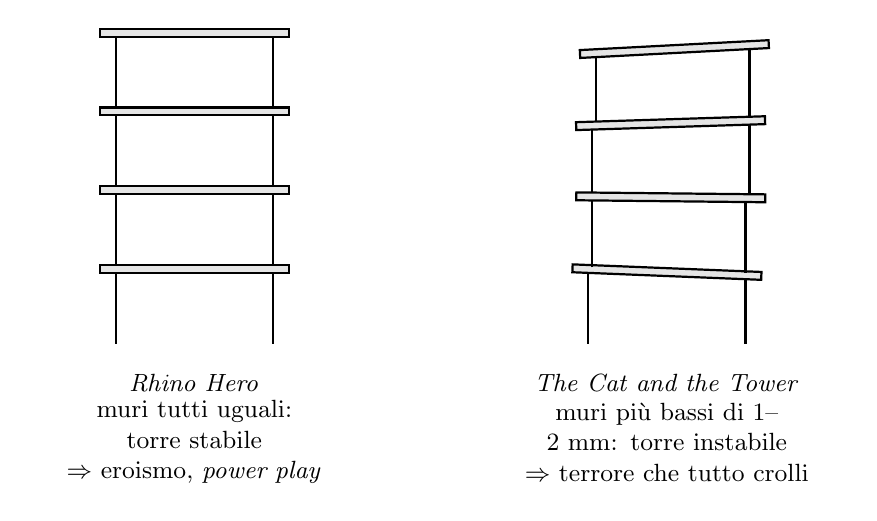
\begin{tikzpicture}[font=\small, x=1cm, y=1cm]
  % Rhino Hero: piani regolari
  \begin{scope}[shift={(0,0)}]
    \foreach \y in {0,1,2,3}{
      \draw[thick] (0,\y) -- (0,\y+0.9);
      \draw[thick] (2,\y) -- (2,\y+0.9);
      \draw[thick, fill=gray!20] (-0.2,\y+0.9) rectangle (2.2,\y+1.0);
    }
    \node[align=center] at (1,-0.5) {\emph{Rhino Hero}};
    \node[align=center, text width=4cm] at (1,-1.25)
      {muri tutti uguali: torre stabile\\$\Rightarrow$ eroismo, \emph{power play}};
  \end{scope}
  % Cat and Tower: muri di altezze diverse
  \begin{scope}[shift={(6,0)}]
    \draw[thick] (0,0) -- (0,0.9);   \draw[thick] (2,0) -- (2,0.82);
    \draw[thick, fill=gray!20, rotate around={-2.3:(0,0.9)}] (-0.2,0.9) rectangle (2.2,1.0);
    \draw[thick] (0.05,0.97) -- (0.05,1.82); \draw[thick] (2.0,0.9) -- (2.0,1.8);
    \draw[thick, fill=gray!20, rotate around={-0.6:(0.05,1.82)}] (-0.15,1.82) rectangle (2.25,1.92);
    \draw[thick] (0.05,1.92) -- (0.05,2.72); \draw[thick] (2.05,1.9) -- (2.05,2.78);
    \draw[thick, fill=gray!20, rotate around={1.8:(0.05,2.72)}] (-0.15,2.72) rectangle (2.25,2.82);
    \draw[thick] (0.1,2.82) -- (0.1,3.64); \draw[thick] (2.05,2.88) -- (2.05,3.78);
    \draw[thick, fill=gray!20, rotate around={3.0:(0.1,3.64)}] (-0.1,3.64) rectangle (2.3,3.74);
    \node[align=center] at (1,-0.5) {\emph{The Cat and the Tower}};
    \node[align=center, text width=4.4cm] at (1,-1.25)
      {muri più bassi di 1--2 mm: torre instabile\\$\Rightarrow$ terrore che tutto
      crolli};
  \end{scope}
\end{tikzpicture}
\caption{Stessa meccanica, paragame diverso: due torri di cartone. In \emph{Rhino Hero}
i piani sono regolari e la dinamica è quella dell'eroe che sale; in \emph{The Cat and
the Tower} alcuni muri sono di uno o due millimetri più bassi, e la torre, sempre
storta, trasmette paura e fragilità. Schema illustrativo, con le pendenze esagerate.}
\label{a10:fig:torri}
\end{figure}

% ---------------------------------------------------------------------
\section{Chiusura: ci si vede il 12}
\label{a10:sec:chiusura}

Mancano tre minuti, ``tempo per un'ultima domanda'', magari ``quella nell'angolino, un
po' timida''. Non arriva (``adesso non ce la faccio''). Gianmarco si smuta, ``il segnale
internazionale'' di chi sta per salutare, ma non ha domande; Ruggero lo invita
scherzosamente a dire anche solo ``cose stupide, tipo: oggi ho ucciso una mosca in
bagno''.

``Allora, gente, io vi saluto, e la lezione di oggi si conclude così.'' L'appuntamento è
\textbf{il 12}, con i \emph{pitch}: ``non fate scherzi, so che li avete, so che li potete
fare''. Al \emph{pitch} non ci sarà solo Ruggero: ci saranno anche \textbf{Beatrice} e
\textbf{Daniele}. ``Buona serata, buona cena, buon weekend.''

% ---------------------------------------------------------------------
\section*{Punti chiave del capitolo}
\addcontentsline{toc}{section}{Punti chiave del capitolo}

\begin{itemize}
  \item La \textbf{UX} è un primo strato tra la persona che si avvicina al gioco e
        l'ecosistema di regole: può essere ``un incredibile aiuto o un gigantesco
        ostacolo''. Regole perfette che non arrivano a chi gioca finiscono ``nel
        cestino''.
  \item I \textbf{quattro pilastri}: \textbf{immediatezza} (si capisce subito, senza
        sforzo: spade e scudi, il barile di petrolio, l'alloro dei punti vittoria),
        \textbf{efficienza} (un'azione complessa nel minor spazio: ``pesca una carta''),
        \textbf{memorabilità} (il +4 di \emph{Uno}, il simbolo di ``tappare'' di
        \emph{Magic}), \textbf{soddisfazione} (\emph{Parks}, \emph{Canvas}, \emph{Tiny
        Epic Mechs}). Sono indipendenti: le icone di \emph{Race for the Galaxy} sono poco
        immediate ma molto efficienti.
  \item Immediato per chi gioca abitualmente non vuol dire immediato per tutti; anche il
        \textbf{colore} fa parte del significato di un'icona.
  \item Il \textbf{wireframe} delle carte cambia durante il prototipo: togliere ciò che
        vale zero, ridurre il testo con le icone, spostare ciò che conta meno. Nei primi
        stadi: \textbf{carte funzionali, non carte belle}.
  \item \textbf{Accessibilità}: font per la dislessia, \emph{curb cut effect} (ciò che è
        più accessibile per qualcuno lo è per tutti), daltonismo da verificare con
        \textbf{Chromatic Vision Simulator}; i mancini e le carte a ventaglio.
  \item Il \textbf{paragame} estende al gioco il \textbf{paratesto}: tutto ciò che non è
        regole e non è fiction, ma incide sull'esperienza. I bordi sono zone grigie
        (i librogame, \emph{Lift It}).
  \item Le aree: \textbf{materialità} (legno, plastica, metallo, app, spessore e
        \emph{core} delle carte, \emph{standee}; clessidra contro timer),
        \textbf{formato} (font, misura delle carte, \emph{200 Word RPG}),
        \textbf{regolamento} (pagine, più libretti, video, glossario,
        \emph{playthrough}, \emph{play aid}), \textbf{scatola} (dall'armadio alla
        Kallax), \textbf{grafica e illustrazioni} (due mestieri diversi),
        \textbf{interfaccia analogica}, \textbf{ambiente} (il tavolo IKEA, il treno,
        \emph{Jenga} in aereo), \textbf{audio}, \textbf{contesto}, \textbf{lingua},
        \textbf{spazio urbano e ibridi digitali}, \textbf{inserti e setup}.
  \item Il paragame \textbf{incide sulle regole}: il formato limita la complessità
        delle regole, la clessidra cambia la tensione, la colonna sonora può essere una
        meccanica. Ai \emph{pitch} e alle revisioni Ruggero chiederà
        \textbf{``tantissimi perché''}.
  \item I casi studio vanno da \emph{Cuba Libre} (due regolamenti, diagrammi di flusso
        per i bot, brochure per fazione) a \emph{193 Days} (solo un mazzo), da
        \emph{Shenzhen I/O} (il manuale stampato) a \emph{Meltdown} (tessere di
        ghiaccio). Il test: ``\textbf{poteva essere di cartone?}''
  \item Il paragame non agisce direttamente sulle dinamiche: agisce sulle meccaniche
        (e sulla fiction), come tutto il design. Serve a far sì che \textbf{le intenzioni
        di design arrivino} a chi gioca, anche quando chi l'ha progettato non è al
        tavolo.
  \item Gli \textbf{inserti} non sono un dettaglio: nessuno ama il \emph{setup}, e un
        buon inserto lo accorcia. Il \emph{setup} si può anche rendere parte del gioco,
        nei giochi leggeri.
  \item \textbf{Ricerca e sviluppo} anche sul paragame: \emph{Rhino Hero} e \emph{The
        Cat and the Tower} hanno la stessa meccanica, ma muri di altezza diversa
        trasformano l'eroismo in terrore. \emph{Copy, transform, combine}, e
        \textbf{cross-modalità}.
\end{itemize}

%    % =====================================================================
%  Analog Game Design, lezione 11 — Il pitch dei progetti di gruppo.
%  Una lezione senza slide e senza lezione frontale: i tre gruppi del
%  corso presentano in tre minuti l'idea del gioco che svilupperanno
%  fino a dicembre, e i tre docenti (Daniele, Beatrice e Ruggero) fanno
%  domande, si ritirano a discutere in privato e poi restituiscono i
%  feedback. In apertura, l'attesa e le regole del pitch. Poi i tre
%  pitch, ciascuno con le sue domande: Murder Memory (escape room
%  investigativa da tavolo a squadre), La Peste (party game a ruoli
%  segreti ispirato alla Maschera della Morte Rossa), un gioco di ruolo
%  in solitario deck building, roguelike e journaling. Dopo la camera
%  di consiglio: la premessa ai feedback (indicazioni, non consigli; il
%  regolamento di massima per il 6 novembre), la domanda di Tiziana su
%  che cosa sia un regolamento in una escape room, i feedback gruppo
%  per gruppo con i casi studio assegnati, il legame tra obiettivo e
%  agency, il perché dei tre minuti, i giochi "generalisti". Infine le
%  domande aperte: scrivere il gioco per chi lo gioca senza di voi, la
%  curse of knowledge, la vergogna delle idee, e una lunga discussione
%  su roguelike, RNG e narrativa modulare (partire dalle emozioni, non
%  dai perk; le meccaniche come metafore; l'ortogonalità).
%  Fonte: trascrizione dell'undicesima lezione (AGD11) del corso breve
%  di Analog Game Design, seconda edizione: una lezione online di circa
%  tre ore, lunedì 12 ottobre 2026, condotta da Daniele con Beatrice e
%  Ruggero.
%  Pacchetti richiesti nel preambolo del libro (già presenti nel
%  main.tex): \usepackage{booktabs}, \usepackage{tikz} con
%    \usetikzlibrary{shapes.geometric,shapes.symbols,shapes.misc,
%      arrows.meta,positioning,calc,fit}
%  (le librerie vanno caricate nel preambolo, non nel capitolo).
%  Consigliati, come per gli altri capitoli: \usepackage[italian]{babel}
%  e \usepackage[T1]{fontenc} (il capitolo compila anche senza).
%
%  Collocazione nel libro: parte "Analog Game Design", undicesimo
%  capitolo (numerazione propria 2.11). Nel file principale del libro,
%  subito dopo il capitolo 2.10:
%
%    \input{AGD/AGD10_ux_design_e_paragame}
%    \input{AGD/AGD11_pitch_e_feedback}
%
%  Tutte le etichette di questo capitolo hanno il prefisso "a11:"
%  (a11:cap:..., a11:sec:..., a11:fig:..., a11:tab:...). Il capitolo è
%  autonomo: non contiene \ref verso altri capitoli.
%  Le figure e le tabelle sono ricostruzioni schematiche di quanto
%  detto a voce (la lezione non ha slide dei docenti), non copie delle
%  slide dei gruppi. Dove la trascrizione è troppo rovinata per
%  ricostruire un dettaglio (un nome di gioco, chi sta parlando), il
%  capitolo lo dice invece di inventarlo.
% =====================================================================

\chapter[Il pitch dei progetti di gruppo]{Il pitch dei progetti di gruppo: tre
giochi, tre minuti, e i feedback di chi li dovrà giocare}
\label{a11:cap:pitch}

Questa è l'\textbf{undicesima lezione} del corso di \textbf{Analog Game Design}, ed è
diversa da tutte le precedenti. ``Non abbiamo slide, non abbiamo una lezione, nel senso
di lezione frontale'': oggi è il giorno del \textbf{\emph{pitch}}, quello che Ruggero, a
fine della lezione sul paragame, aveva dato per certo come ``il 12'', che ``sta nella
pietra''. I tre gruppi di lavoro del corso presentano in \textbf{tre minuti} l'idea del
gioco che svilupperanno fino a dicembre; dopo ogni presentazione i docenti fanno
qualche minuto di domande, poi il gruppo esce dalla stanza virtuale e i docenti
discutono in privato. Quando tutti e tre i gruppi hanno presentato, la seconda metà della
lezione è dedicata ``solo ai feedback, esclusivamente ai feedback''.

I tre progetti sono molto diversi tra loro. Il primo, \textbf{\emph{Murder Memory}}, è
una \emph{escape room} investigativa da tavolo in cui due squadre, la polizia e un
indiziato che ha perso la memoria, risolvono enigmi in parallelo fino a un
interrogatorio finale. Il secondo, \textbf{\emph{La Peste}}, è un \emph{party game} a
ruoli segreti, di deduzione e \emph{bluff}, ambientato nel ballo della \emph{Maschera
della Morte Rossa} di Edgar Allan Poe: a ogni rintocco dell'orologio si balla, ci si
scambiano le carte e la malattia si diffonde. Il terzo è un \textbf{gioco di ruolo in
solitario}, \emph{deck building}, \emph{roguelike} e di \emph{journaling}: si
sopravvive il più a lungo possibile tenendo in equilibrio corpo, mente e status
sociale di un personaggio, e alla fine della partita resta la sua storia, da scrivere.

I feedback sono franchi, e i docenti lo dicono subito: non saranno ``consigli'' ma, dove
l'esperienza dice che un gruppo si sta infilando in un ``ginepraio troppo grosso per il
periodo di tempo che avete'', \textbf{indicazioni} precise (``non fate questo, fate
questo''). I temi che ritornano per tutti e tre i gruppi sono pochi e molto concreti:
\textbf{convergere} su un'idea e uno \emph{scope} realizzabili, \textbf{scrivere il
regolamento} (``il vostro gioco lo devono poter giocare altre persone che non sono
voi''), collegare l'\textbf{obiettivo} di chi gioca a ciò che fa \textbf{turno per
turno}, partire dalle \textbf{emozioni} e non dai bilanciamenti, e usare i
\textbf{casi studio} come strumenti di \emph{problem solving}, non come modelli da
copiare. Ogni gruppo riceve una lista di giochi da studiare, in tutto più di quindici
titoli (tabella~\ref{a11:tab:reference}). L'ultima parte della lezione, aperta alle
domande, diventa una lunga discussione su \emph{roguelike}, generazione casuale e
narrativa modulare, temi che due dei docenti praticano per mestiere.

La lezione è \textbf{online}, su Zoom, e si tiene \textbf{lunedì 12 ottobre
2026}\footnote{La data è quella fissata nella lezione precedente (``il 12 sta nella
pietra'', e ``lunedì'' sono i \emph{pitch}). In questa lezione Daniele ricorda che
Gianmarco ``di solito lunedì arriva un'ora dopo per motivi di lavoro''.}, presumibilmente
dalle 17 alle 20 come le altre: Daniele, che arriva ``da sei ore di lezioni'', ne fa
``altre tre di fila'' e a fine serata parla della sua ``nona ora''. La conducono insieme
i tre docenti del corso: \textbf{Daniele}, che scandisce i tempi, fa partire il timer e
gestisce la sala d'attesa; \textbf{Beatrice} (``Bea''); e \textbf{Ruggero}. Gli studenti
sono divisi in tre gruppi: \textbf{Tiziana}, \textbf{Angelo} e \textbf{Lorenzo L.}
(\emph{Murder Memory}); \textbf{Tancredi}, \textbf{Gianmarco} e \textbf{Lorenzo}
(\emph{La Peste})\footnote{Nel corso ci sono due Lorenzo, e la trascrizione li
distingue solo in un punto, quando Daniele presenta il primo gruppo come ``Tiziana,
Lorenzo L. e Angelo''. L'altro Lorenzo è nel gruppo di Tancredi e Gianmarco (``io sono
con Gianmarco e Lorenzo'', dice Tancredi). Il capitolo scrive ``Lorenzo L.'' per il
primo e ``Lorenzo'' per il secondo.}; \textbf{Giordano}, \textbf{Nicola} e
\textbf{Rita} (il \emph{roguelike} in solitario)\footnote{Il nome di Rita è storpiato in
``Verità'' (``Giordano, Nicola, Verità'') e in ``Piano'' (``Rita, Piano e Nicola''); il
contesto e un successivo ``ha ragione anche Rita'' lo rendono sicuro.}.

Tre avvertenze di lettura, le stesse dei capitoli precedenti. La prima: la trascrizione è
automatica e storpia moltissimi nomi. Ruggero diventa ``Ruger'', ``Rugger'',
``Brugger'' e ``Rugg''; \emph{Murder Memory} diventa ``Merd Memory'', ``Mordor
Memory'', ``Marder Memory'' e ``Mordere Memory''; \emph{Lupus in Tabula} è ``Lupus in
Fabula'', ``l'Opus in Fabula'' e ``l'upus in tabula''; \emph{Slay the Spire} è ``Slade
of Spire'', ``Slade Spire'', ``Zade Spyder'' e ``As Lady Spire 2''; \emph{Reigns} è
``Rains'', ``Rain'' e ``Reins''; \emph{The Quiet Year} è ``The Quiet Ear'', ``White
Tier'', ``quai tier'' e ``quietire''; \emph{Inhuman Conditions} è ``In Human
Condition'', ``Unicondition'' e ``Non è un Condition''; Tabletop Simulator è ``Temporal
Simulator'' e ``Voltoltor Simulator''. Dove la ricostruzione è sicura, o molto probabile,
il capitolo usa la forma corretta e lo segnala in nota la prima volta; dove non lo è,
riporta la forma della trascrizione e lo dice. La seconda: con tre docenti e dieci
studenti che parlano spesso uno sull'altro, la trascrizione quasi mai segnala chi sta
parlando, e in più punti ripete due volte la stessa frase (un artefatto del
riconoscimento vocale, che il capitolo ignora). Il capitolo attribuisce le frasi quando
il contesto lo rende chiaro (chi viene chiamato per nome, chi dice ``io sto creando un
\emph{roguelike}'', chi ha scansionato un libro) e resta generico altrimenti. La terza:
le slide dei gruppi non sono nella trascrizione; il capitolo ricostruisce i giochi da ciò
che i gruppi dicono a voce, nelle presentazioni e nelle risposte.

\paragraph{Come leggere questo capitolo.} I tre progetti sono descritti per come sono
stati presentati il 12 ottobre: idee in fase embrionale, con parti ``ancora da
definire'' che i gruppi stessi segnalano. Il capitolo non le completa e non le corregge:
riporta le domande che i docenti fanno, le risposte, e poi i feedback. Le figure
ricostruiscono gli schemi che emergono dal discorso (la procedura del \emph{pitch}, il
round della \emph{Peste}, il legame tra obiettivo e \emph{agency}, il calendario fino a
dicembre); le tabelle riassumono i progetti e i casi studio. Qua e là, dei paragrafi di
\textbf{approfondimento} collegano la lezione ai libri di game design di riferimento
(soprattutto \emph{The Art of Game Design} di Jesse Schell e \emph{A Theory of Fun} di
Raph Koster) e a qualche nozione di psicologia della comunicazione; sono segnalati come
tali e non fanno parte della lezione.

Il percorso del capitolo segue quello della lezione:
\begin{enumerate}
  \item l'attesa, la logistica e le \textbf{regole del \emph{pitch}} (sezioni
        \ref{a11:sec:attesa} e~\ref{a11:sec:regole});
  \item i tre \emph{pitch}, ciascuno con le sue domande: \emph{Murder Memory},
        \emph{La Peste}, il \emph{roguelike} di \emph{journaling} (sezioni
        da~\ref{a11:sec:murder} a~\ref{a11:sec:roguelike});
  \item dopo la camera di consiglio, la \textbf{premessa ai feedback} e la domanda su
        \textbf{che cos'è un regolamento} (sezioni \ref{a11:sec:premessa}
        e~\ref{a11:sec:regolamento});
  \item i \textbf{feedback} gruppo per gruppo, con i casi studio (sezioni
        da~\ref{a11:sec:fbmurder} a~\ref{a11:sec:reference});
  \item le \textbf{domande aperte}: il regolamento come strumento di test, la
        \emph{curse of knowledge}, la vergogna delle idee (sezioni
        \ref{a11:sec:testing} e~\ref{a11:sec:vergogna});
  \item la discussione su \textbf{\emph{roguelike}, RNG e narrativa modulare}, e la
        chiusura (sezioni da~\ref{a11:sec:rng} a~\ref{a11:sec:chiusura}).
\end{enumerate}

% ---------------------------------------------------------------------
\section{L'attesa: una ``quotina di ansia''}
\label{a11:sec:attesa}

I primi a collegarsi sono Angelo, Nicola, Lorenzo e Rita; Beatrice e Ruggero sono già
in stanza. Daniele ``arriva un attimino in ritardo perché sta chiudendo un'altra
lezione''. La prima domanda è quella di sempre, ``come state? come vi sentite oggi?'', e
la risposta di uno studente riassume l'umore della classe: ``leggermente preoccupato
per il \emph{pitch}, ma se no tranquillo''. ``Anch'io, è normale'', gli risponde
Beatrice: ``ogni presentazione ha una quotina di ansia''. Lei, dice, è ``molto curiosa''
e ``abbastanza fiduciosa che usciranno bellissimi \emph{pitch}'': ``non preoccupatevi,
siamo proprio in ascolto anche per darvi una mano dove possiamo''. Poi va a prendere
``il mio quadernino di appunti, così mi segno le cose''.

In attesa dei ritardatari, i docenti aprono come al solito lo spazio per le domande,
magari di chi ha recuperato la lezione precedente. Uno studente la sta finendo di
recuperare: ``è una figata pazzesca''. Ruggero conferma che ``sulla questione del
paragame c'è tantissimo da dire'' e spera che abbia dato ``qualche spunto''. Poi spiega
la logistica, che ``già dovreste sapere'': niente slide e niente lezione frontale; ``oggi
vediamo i vostri \emph{pitch} e dedichiamo il tempo a ciascun gruppo''. Si corregge
subito dopo un lapsus (``dedichiamo il gruppo a ciascun tempo. Chi può dirlo? Qualcuno
finirà nell'800, qualcuno finirà nel 2000''). L'idea è di dare ai gruppi dei feedback
``in base anche al vostro \emph{pitch}''.

Arriva Daniele, accolto con un ``grazie in fanfare'': viene ``da sei ore di lezioni''
(``e invece adesso guarda, ne fai altre tre di fila''; ``Madonna, Daniele, ci lasci le
penne. Non svenire''). È lui a segnare le presenze. Arriva Tiziana, poi Tancredi. Mentre
manda ``due messaggi di lavoro'', Daniele dà un consiglio organizzativo: decidete ``dietro
le quinte'' l'ordine di presentazione dei gruppi, altrimenti lo sceglieranno i docenti.
Un vincolo c'è già: il gruppo di \textbf{Gianmarco}, Tancredi e Lorenzo va lasciato per
ultimo, perché Gianmarco il lunedì arriva circa un'ora dopo per lavoro (``tra una
quarantina di minuti massimo''). Un altro vincolo arriva da una studentessa del primo
gruppo, che deve staccarsi dieci minuti prima per prendere il treno delle otto: il suo
gruppo, se i compagni sono d'accordo (``Sì, sì, va bene''), può andare per primo. E
così si fa: ``iniziamo voi''.

Nel frattempo, il silenzio. ``Avremo l'\emph{horror vacui}'', scherza Ruggero: ``se
nessuno fa domande, io non so gestire. Daniele, cosa devo fare? Come faccio?''. Mancano
soltanto Giordano e Gianmarco; Daniele chiede di avvisarlo se entrano mentre i gruppi
presentano, così da non perdere le loro presenze.

C'è un ultimo intoppo tecnico, quello di ogni lezione online: la condivisione dello
schermo da un Mac (``il problema sempre del Mac per le autorizzazioni''). Daniele
sospetta un aggiornamento di Zoom (``e l'aula è diversa, tra l'altro: voi non ve ne
rendete conto, ma è un'aula differente''), ma alla fine la presentazione del primo
gruppo parte, in modalità ``presenta'', a schermo intero, con le frecce della tastiera
per andare avanti.

% ---------------------------------------------------------------------
\section{Le regole del \emph{pitch}}
\label{a11:sec:regole}

Prima di cominciare, Daniele ripete ``bene le regole del \emph{pitch} di oggi''
(figura~\ref{a11:fig:procedura}).

\begin{itemize}
  \item \textbf{Tre minuti.} Daniele fa partire un timer, conta ``3, 2, 1, via'', e il
        gruppo spiega ``tutto''. Chi va oltre non viene interrotto (``vi faccio
        finire''), ma alla fine si sentirà dire se è andato ``troppo lungo'' o ``troppo
        corto'', ``perché comunque sapevate che più o meno il tempo era quello''. Il
        tempo è uguale per tutti: ``non possiamo dare la possibilità a ogni team di
        avere più tempo rispetto agli altri. Altrimenti, è un casino''.
  \item \textbf{Due o tre minuti di domande} da parte di Daniele, Ruggero e Beatrice
        (``comunque quanto tempo ci mettono'').
  \item \textbf{La sala d'attesa.} Il gruppo esce da Zoom e rientra: Daniele ha
        attivato la sala d'attesa. I tre docenti si prendono ``qualche appunto in
        privato di confronto, senza essere registrati'', e poi riammettono tutti.
        Quando una studentessa chiede se la sala d'attesa sia ``una stanza che c'è
        veramente'', la risposta è che è ``l'anticamera'' di Zoom, dove però non si
        può parlare: chi vuole chiacchierare nel frattempo ha un canale vocale
        ``Analog Game Design'' sul Discord del corso.
  \item Si fa così per tutti i gruppi. La parte dei \emph{pitch} ``di solito dura
        un'ora, un'ora e mezza''; poi ``vi diamo i feedback e vi diamo anche dei
        consigli su cosa fare, perché poi dovrete svilupparle, 'ste robe''.
  \item \textbf{Il materiale.} Dopo ogni presentazione il gruppo condivide in chat il
        link alle slide (``Condividi'', ``chiunque abbia il link'', copia, incolla) e
        carica tutto nella cartella \emph{project work} del proprio gruppo.
\end{itemize}

Il primo gruppo avverte che improvviserà (``non ci siamo preparati sulla
presentazione''). Nessun problema, ma conviene che parli una persona sola, se ne ha una
che ``sa tutto quanto''; gli altri intervengono se manca qualcosa. Le domande dei
docenti, durante il primo \emph{pitch}, si allungano: alla fine il primo gruppo occupa
venti minuti, e Daniele stabilisce per gli altri ``venti minuti più o meno a team''.
Nessun feedback a caldo, nemmeno per chi deve andarsene prima: i docenti vogliono prima
``vedere il livello di tutti'', ``cosa hanno prodotto tutti''.

\begin{figure}[htbp]
\centering
\begin{tikzpicture}[
  font=\small,
  a11step/.style={draw, thick, rounded corners=3pt, minimum height=1.2cm,
               text width=2.3cm, align=center},
  a11priv/.style={draw, thick, dashed, rounded corners=3pt, fill=gray!15,
               minimum height=1.2cm, text width=2.3cm, align=center},
  a11arr/.style={-{Stealth[length=3mm]}, thick}
]
  \node[a11step] (a) {\textbf{Pitch}\\3 minuti\\a timer};
  \node[a11step, right=0.6cm of a] (b) {\textbf{Domande}\\2--3 minuti\\dei docenti};
  \node[a11priv, right=0.6cm of b] (c) {\textbf{Sala d'attesa}\\appunti dei\\docenti, non
    registrati};
  \node[a11step, right=0.6cm of c] (d) {\textbf{Rientro}\\e prossimo\\gruppo};
  \draw[a11arr] (a) -- (b);
  \draw[a11arr] (b) -- (c);
  \draw[a11arr] (c) -- (d);
  \draw[a11arr, rounded corners=4pt] (d.south) -- ++(0,-0.7) -| node[pos=0.25, below,
    font=\footnotesize]{per ognuno dei tre gruppi (circa 20 minuti a gruppo)} (a.south);
  \node[a11step, below=1.9cm of c, text width=5.2cm, fill=gray!5] (f)
    {\textbf{Seconda metà della lezione}\\feedback di gruppo, feedback di classe,
     domande aperte};
  \draw[a11arr, dashed] (d.east) -- ++(0.4,0) |- (f.east);
\end{tikzpicture}
\caption{La procedura del \emph{pitch} come la descrive Daniele. I feedback non arrivano
a caldo: i docenti li danno solo dopo aver visto tutti e tre i gruppi.}
\label{a11:fig:procedura}
\end{figure}

\paragraph{Approfondimento: il \emph{pitch} come prova di comunicazione.} Il formato
non è arbitrario, e Daniele lo spiegherà più avanti (sezione~\ref{a11:sec:fbpeste}):
tre minuti sono più o meno il tempo che un editore o un passante in fiera concede a
un'idea. Ma il \emph{pitch} è anche il primo momento in cui il gioco esce dalla testa del
gruppo e arriva a qualcuno che non c'era quando è stato pensato. Schell, in \emph{The Art
of Game Design}, dedica a questo passaggio un capitolo intero (``The Designer Gives the
Client a Pitch''), con l'idea di fondo che presentare un gioco serve anche a chi lo
presenta: costringe a scegliere che cosa, del gioco, conta davvero. Le domande dei docenti che seguono ogni \emph{pitch} di questa lezione
sono, in gran parte, la verifica di questo: che cosa faccio, io che gioco, in questo
momento?

% ---------------------------------------------------------------------
\section{Primo \emph{pitch}: \emph{Murder Memory}}
\label{a11:sec:murder}

Il primo gruppo è quello di \textbf{Tiziana}, \textbf{Lorenzo L.} e \textbf{Angelo}.
Presenta Tiziana, con l'accordo dei compagni, che interverranno se lei dimentica
qualcosa. Beatrice è ``già curiosissima di questo \emph{Murder Memory}'', e quando
lascia scappare un ``ho visto che è un gioco di carte'' viene fermata: ``non ci si
spoilera''. ``3, 2, 1, via.''

\subsection{Il \emph{pitch}}

\emph{Murder Memory} è ``una \emph{escape room} investigativa da tavolo'' (``ci siamo
dimenticati di precisare questa cosa, ma sarà da tavolo''). Chi gioca si trova coinvolto
in una \textbf{festa nella villa di un ricco proprietario}, durante la quale uno degli
invitati viene ucciso. Il principale indiziato è un altro invitato, che ha perso i sensi
e si sveglia \textbf{senza memoria}.

È un gioco \textbf{competitivo e cooperativo} insieme: due squadre si affrontano per
arrivare alla verità entro un \textbf{tempo limitato}, cooperando al loro interno.
\begin{itemize}
  \item Una squadra interpreta l'\textbf{indiziato} che ha perso la memoria. Non ricorda
        chi è né che cosa sia successo; potrebbe essere l'assassino e non saperlo. Si
        nasconde dalla polizia mentre cerca la verità, il che lo rende ancora di più il
        principale indiziato. ``Enigma dopo enigma'' deve scoprire chi è e svelare il
        mistero: ``è davvero lui il colpevole, o è solo un'altra vittima?''. Ogni
        giocatore della squadra potrebbe interpretare \textbf{un aspetto diverso della
        stessa persona}: è una cosa ``ancora da definire'', perché il gruppo non sa
        ancora se riuscirà a realizzarla in concreto.
  \item L'altra squadra interpreta i \textbf{poliziotti}, chiamati dal proprietario.
        Seguono le indagini, cercano indizi e interrogano gli invitati e il
        proprietario della villa, anche a proposito dell'indiziato che non riescono a
        trovare.
\end{itemize}

La struttura è una \textbf{successione lineare di enigmi}, che guida ciascuna squadra
alla risoluzione finale; la risoluzione prevede un \textbf{confronto diretto} tra le due
squadre, attraverso un \textbf{interrogatorio}. Il gruppo vorrebbe diversificare il più
possibile gli enigmi della successione, così da far partecipare più giocatori.
L'obiettivo dell'indiziato è scoprire la verità su se stesso e su ciò che è successo;
quello dei poliziotti, trovare il colpevole.

L'obiettivo del gruppo, come designer, è ``esprimere noi stessi ed esplorare nuove
tipologie di gioco'', fondendo elementi investigativi e di gioco di ruolo con la
struttura dell'\emph{escape}; e ``non ci dispiacerebbe pubblicarlo''. Le
\textbf{emozioni} che vogliono suscitare sono \textbf{incertezza}, \textbf{scoperta},
un'esperienza \textbf{adrenalinica}, \textbf{sorpresa} e \textbf{ansia}. Chiude una
battuta (``prenotatevi per provarlo, nessuno vi picchierà'') e la presentazione dei
membri del gruppo, ognuno con un nome da personaggio\footnote{La trascrizione riporta
``siamo Lorenzo, la Pomarda, Angelo, Tenente Colombo e io, Tiziana Carabayt'': almeno
``Tenente Colombo'' è chiaramente un soprannome scherzoso a tema investigativo; le
altre parole non sono ricostruibili con sicurezza.}.

Tempo: \textbf{tre minuti e quattordici secondi}. ``Direi che siamo comunque in
\emph{time}'', commenta Daniele: con un po' più di velocità ci sarebbero stati
tranquillamente.

\subsection{Le domande}

\paragraph{Come si vince?} Daniele parte con un apprezzamento e un dubbio. ``Lato
emotivo, molto bene'': le emozioni sono chiare. ``Lato meccanico, ho un po' di dubbi.''
Non è chiaro se il gioco abbia un \textbf{\emph{endgame} predefinito}, cioè se a livello
meccanico si vinca o si perda (``com'è che so se ho vinto o se ho perso?''), o se vada
``nella direzione più RPG'', in cui conta non chi vince ma ``avere un epilogo
strutturato''.

\paragraph{Chi risolve gli enigmi?} Un'altra domanda, più pragmatica, arriva dai docenti
insieme: le squadre sono due, ma gli enigmi chi li risolve? Insieme? Una squadra sola
mentre l'altra aspetta? (``Hanno due serie diverse.'') Il punto, chiarisce chi chiede, è
che non è chiaro ``che cosa faccio, in base al ruolo in cui sono'', e con quale obiettivo
personale al tavolo. Gli studenti non sapevano se dovessero entrare in questo dettaglio
nel \emph{pitch}; la risposta dei docenti è: se la risposta c'è, ditela; se non c'è,
``non generatela adesso''.

La risposta c'è. Gli enigmi procedono \textbf{in contemporanea}, con lo stesso tempo per
entrambe le squadre. I poliziotti hanno tutte le informazioni se riescono ad arrivare
alla fine del loro percorso; l'indiziato, arrivando alla fine del suo o il più vicino
possibile, ottiene informazioni su se stesso. \textbf{Allo scadere del tempo} le due
squadre si confrontano: i poliziotti fanno all'indiziato delle domande ``ovviamente
previste'', e l'indiziato saprà rispondere più o meno correttamente a seconda di quanto
ha scoperto. Se non sa chi è, ``rischia di rimanere un po' così'' su certe domande:
può inventarsi le risposte, ma rischia di non essere coerente. Ne nascono diversi esiti
(tabella~\ref{a11:tab:esiti}).

\begin{table}[htbp]
\centering
\small
\begin{tabular}{@{}p{5.6cm}p{7.4cm}@{}}
\toprule
\textbf{Situazione allo scadere del tempo} & \textbf{Esito (come descritto nel
\emph{pitch})} \\
\midrule
Entrambe le squadre arrivano alla fine del percorso & ``vincono entrambi'': i
poliziotti hanno gli elementi per capire chi è il vero colpevole, e l'indiziato sa
rispondere \\
I poliziotti arrivano alla fine, l'indiziato no & vincono i poliziotti: l'indiziato non
risponde correttamente alle domande e viene arrestato \\
L'indiziato ottiene le informazioni su di sé & l'indiziato vince: risponde correttamente
e viene scagionato \\
\bottomrule
\end{tabular}
\caption{Gli esiti dell'interrogatorio finale di \emph{Murder Memory}, come li descrive
Tiziana rispondendo alle domande. Il gruppo li presenta come idea ancora aperta.}
\label{a11:tab:esiti}
\end{table}

\paragraph{Quanti giocatori?} Daniele ha ``due domande molto brevi''. La prima: per
quanti giocatori è il gioco? Minimo due, uno per squadra; il gruppo pensava a un massimo
di \textbf{quattro per squadra}. Si interpretano solo i membri delle squadre? Sì: gli
invitati sono \textbf{NPC}. La seconda domanda, a Daniele, sfugge (``la sto perdendo?
Arrivo''); Beatrice lo rassicura (``è normale, poi tornano le domande mentre si
parla'') e prende la parola.

\paragraph{L'indiziato vuole scagionarsi o sapere la verità?} Beatrice ha ``tantissime
domande'' e ne seleziona alcune. La prima: la squadra dell'indiziato ha più lo scopo di
scagionarsi o di ricostruire la verità? Deve scoprire la verità su se stesso, risponde
Tiziana: scoprendo chi è, può affrontare i poliziotti. Beatrice chiede allora conferma
di un punto di design: si parte dall'idea che l'indiziato \textbf{non è colpevole}?
Corretto: non è colpevole, ``però non lo sa''.

\paragraph{Le sfaccettature dell'indiziato.} La seconda domanda di Beatrice riguarda le
``varie modalità di essere'' dell'indiziato, una per giocatore. Come funzionerà? Il
dubbio di Beatrice è più ampio: ``avete tanta carne al fuoco''. Enigmi, \emph{drive}
narrativi, una storia raccontata in più versioni, una polizia che non è una persona sola.
``Non vi sto invitando per forza a ridurre lo \emph{scope}'', ma ``è bene che abbiate una
direzione e una motivazione per tutte le scelte che prendete''. L'idea dell'indiziato
interpretato da una squadra intera le piace molto, ma non capisce che cosa farà lei,
giocando l'indiziato, oltre al lavoro di ricerca con le altre parti di sé: e quando
dovrà scagionarsi, come funzionerà? ``Compileremo una scheda, oppure parleremo con la
polizia?''. La risposta: la \textbf{mente divisa} era un'ipotesi iniziale, ``quasi
necessaria'' per giustificare più persone che fanno un'unica persona, ma non
obbligatoria, perché ``è nostra intenzione semplificare, non complicarci la vita''.

\paragraph{``Dovete spoilerare''.} A questo punto il gruppo ammette che manca una parte,
taciuta apposta ``perché non volevamo spoilerare''. La reazione dei docenti è immediata:
``Dovete spoilerare. Non siamo giocatori''. Al \emph{pitch} i docenti sono come un
\emph{publisher} a cui si propone un gioco: se non gli si dicono le cose importanti,
``noi come facciamo?''. ``Non lo sapevamo. Scusate.'' ``Tutto bene. Dici tutto adesso.''

Il retroscena è questo. Il \textbf{proprietario} della villa è un \textbf{appassionato di
enigmi} ed è lui \textbf{l'assassino}: ha ucciso uno degli invitati per costruire tutta
la messa in scena, ``fondamentalmente per divertirsi''. È lui a far perdere la memoria
all'indiziato, facendogli bere qualcosa. L'indiziato si sveglia in un punto in cui non è
visto, si accorge che è successo qualcosa (c'è la polizia) e va subito in agitazione:
non ricorda chi è, e se gli fanno una domanda non saprà cosa rispondere. Mentre si
nasconde trova \textbf{un oggetto che gli è familiare}, e da lì parte la serie degli
enigmi. Ha la sensazione di essere \textbf{guidato}, pilotato, che ci sia qualcosa che
non torna, ma ``non è il momento'' di chiederselo. Dall'altra parte, il proprietario
chiama i poliziotti e si diverte anche alle loro spalle: li guida attraverso altri
enigmi, con cui ricostruiscono le informazioni sugli invitati e, attraverso gli invitati,
sull'indiziato che non trovano. ``Scusa, no, è importantissimo'', commentano i docenti.

\paragraph{Storia prefatta o emergente?} Daniele fa un'ultima domanda, ``molto
semplice'': il gioco ha una \textbf{storia prefatta}, definita, che i giocatori stanno
solo scoprendo? Non è una storia emergente? Sì, è prefatta.

\paragraph{I giochi più vicini.} Poi tocca a Ruggero, con una domanda ``apparentemente
dal nulla'', le cui ragioni verranno dette dopo: nella fase di ricerca e sviluppo, quali
sono i giochi più vicini al vostro? Ruggero ne ha già ``due segnati qua'' che ``devono
uscire fuori da questa risposta''. Non è un indovinello, precisa: se i giochi citati dal
gruppo coincidono con i suoi, bene; se sono molto diversi, ``allora ci sono altri
problemi'', perché vuol dire che i docenti hanno capito un'altra cosa. Daniele allarga
la domanda: non serve un gioco unico che spieghi tutto il progetto, che ibrida generi
diversi ed è in gran parte sperimentale (``è molto chiaro quello che ci state
proponendo''); bastano ``un po' di ispirazioni'', e la ricerca e sviluppo ``può essere un
film, può essere una canzone''.

Tiziana racconta l'origine dell'idea: il gruppo ha scelto la proposta di Lorenzo L., un
personaggio che perde la memoria e cerca di ricostruirla, e poi l'interesse comune per
le scelte, per l'\emph{escape} e per gli elementi investigativi. Lei ha cercato giochi
simili ``e non ho trovato niente''; ha giocato investigativi e qualche \emph{escape}, ma
non si è ispirata a nessuno in particolare (``se ci volete dare qualche indicazione,
siamo contenti''). Aggiunge un'idea sua sul formato: dare i percorsi ``in modalità
busta'', con buste da aprire che contengono il testo scritto; ma nel gruppo c'è chi ha
un'idea diversa. ``Quello lo svilupperete dopo''. Lorenzo L., invece, un riferimento ce
l'ha: quando aveva proposto la perdita di memoria, gli era venuto subito in mente un
titolo della serie \textbf{\emph{Hidden Games}}, in cui tutti hanno perso la memoria,
tutti indagano e uno di loro è l'assassino: \emph{Freddo come il
ghiaccio}\footnote{Così nella trascrizione (``Freddo come il ghiaccio. Bravissimo,
Lorenzo''). \emph{Hidden Games} è una serie di giochi investigativi in scatola; il
titolo esatto del caso citato non è verificabile dalla trascrizione.}. ``Bravissimo,
Lorenzo.'' Angelo, a parte le \emph{escape room} giocate (``non particolarmente
tante''), non ha riferimenti: è proprio questo che lo ha spinto ad avvicinarsi al genere.

Sono passati venti minuti, ed è arrivato Gianmarco. Daniele riassume per lui la
procedura (presentazione, domande, sala d'attesa, feedback alla fine) e manda il primo
gruppo in sala d'attesa.

% ---------------------------------------------------------------------
\section{Secondo \emph{pitch}: \emph{La Peste}}
\label{a11:sec:peste}

Visto che Gianmarco è arrivato, il secondo turno tocca al suo gruppo: \textbf{Tancredi},
\textbf{Gianmarco} e \textbf{Lorenzo}. Presenta Tancredi. Prima di partire, però, c'è un
equivoco da chiarire: il gruppo ``non si era orientato per i tre minuti''. Aveva capito
che il \emph{pitch} fosse ``una cosa un po' più lunga'', e ha preparato una struttura ``un
po' più cicciotta'', poi riadattata con alcune slide in appendice. ``Sapevate quanto tempo
ci davamo?'' ``Noi avevamo trenta minuti.'' Daniele si chiede se sia stata colpa sua, ma
ricorda di essere stato chiaro: ``i \emph{pitch} erano da tre minuti, tre o quattro minuti
di solito''. Gli studenti stessi trovavano strano un \emph{pitch} così lungo (``come idea
avevamo tutti in mente un \emph{pitch} che fosse una roba molto veloce''). Il materiale in
più non va buttato: ``tenetelo da parte, che servirà''. E il gruppo, alla fine, sta nei
tre minuti: ``bravissimi''.

\subsection{Il \emph{pitch}}

Il gioco si chiama \textbf{\emph{La Peste}} ed è ambientato nel racconto \emph{La
maschera della Morte Rossa} di Edgar Allan Poe (``ce la posso fare''). È un \textbf{party
game a ruoli segreti}, di \textbf{deduzione e \emph{bluff}}. Uno degli invitati del ballo
rappresenta la malattia, che il gruppo chiama \textbf{Pestilenza}, e il suo obiettivo è
espandersi. A ogni \textbf{rintocco dell'orologio} (scandito da un piccolo timer, che
definisce i round) ci si mette a \textbf{ballare}: durante il ballo i giocatori si
scambiano le carte, e in base alle carte che si hanno in mano alla fine del turno si è
sani o malati. Dopo il ballo c'è la \textbf{fase sociale}, ``quella un po' più caciarona
da \emph{party game}'', in cui ci si accusa e si cerca di capire chi si è ammalato e chi
no.

I \textbf{pilastri} del gioco sono tre: la \textbf{dualità segreta} tra Pestilenza e
Medico, che si combattono senza che nessuno sappia chi sono; la \textbf{malattia che si
espande}; la \textbf{deduzione e il \emph{bluff}}. Le \textbf{emozioni} principali sono
l'\textbf{incertezza} (non sapere bene i ruoli), l'\textbf{ansia} e la
\textbf{preoccupazione}, e l'\textbf{inclusione}: i giocatori malati \textbf{non vengono
eliminati}, come invece ``ogni tanto succede nei giochi di questo tipo''. Il formato è da
\textbf{5 a 8 giocatori}, per circa \textbf{30 minuti} (``ancora un po' da decidere'').

I ruoli sono tre (tabella~\ref{a11:tab:ruoli}). Il \textbf{setup} è a \textbf{buste},
come in \emph{Secret Hitler}\footnote{Nella trascrizione ``Secret Teaser'', poi
``Secreti Hitler''.}: ogni busta è già preparata in base al numero di giocatori e
contiene le carte di chi la riceve. Il gioco si sviluppa in \textbf{sette round}, il
numero dei rintocchi (``va ancora sistemato''); ogni round ha tre fasi: il
\textbf{ballo}, in cui ci si scambiano le carte; la \textbf{risoluzione}, in cui in base
alle carte che si hanno ``succedono cose'' (``tendenzialmente ti ammali''); la
\textbf{fase sociale}, la discussione. Alla fine si guardano le \textbf{condizioni di
vittoria} (figura~\ref{a11:fig:round}).

\begin{table}[htbp]
\centering
\small
\begin{tabular}{@{}p{2.4cm}p{4.6cm}p{6cm}@{}}
\toprule
\textbf{Ruolo} & \textbf{Carte iniziali} & \textbf{Obiettivo e comportamento} \\
\midrule
Pestilenza & una carta \emph{peste}, che trasmette la malattia, e una carta vuota &
l'unico che parte malato; vuole contagiare tutti \\
Medico & due \emph{talismani}, che proteggono dalla malattia (``non ti fa ammalare'') &
combatte la Pestilenza senza farsi riconoscere \\
Cortigiani & solo carte vuote (\emph{invito}) & finché sono sani giocano con il Medico;
quando si infettano passano dalla parte della Pestilenza e vogliono far infettare
tutti \\
\bottomrule
\end{tabular}
\caption{I ruoli della \emph{Peste} come presentati al \emph{pitch}. Le carte vuote,
nella descrizione del \emph{setup}, si chiamano ``invito''.}
\label{a11:tab:ruoli}
\end{table}

\begin{figure}[htbp]
\centering
\begin{tikzpicture}[
  font=\small,
  a11ph/.style={draw, thick, rounded corners=3pt, minimum height=1.2cm,
             text width=2.6cm, align=center},
  a11arr/.style={-{Stealth[length=3mm]}, thick}
]
  \node[a11ph, fill=gray!10] (s) {\textbf{Setup}\\buste preparate per numero di
    giocatori};
  \node[a11ph, right=1.0cm of s] (b) {\textbf{Ballo}\\si scambiano le carte};
  \node[a11ph, right=0.7cm of b] (r) {\textbf{Risoluzione}\\sani o malati, in base alle
    carte in mano};
  \node[a11ph, below=1.3cm of r] (f) {\textbf{Fase sociale}\\accuse, discussione,
    deduzione};
  \node[a11ph, right=1.0cm of f, fill=gray!10] (v) {\textbf{Fine}\\condizioni di
    vittoria};
  \draw[a11arr] (s) -- node[above, font=\footnotesize]{rintocco} (b);
  \draw[a11arr] (b) -- (r);
  \draw[a11arr] (r) -- (f);
  \draw[a11arr] (f.west) -| node[pos=0.25, below, font=\footnotesize]{prossimo
    rintocco (7 in tutto)} (b.south);
  \draw[a11arr, dashed] (f) -- node[above, font=\footnotesize]{dopo il
    7\textsuperscript{o}} (v);
\end{tikzpicture}
\caption{Il ciclo di gioco della \emph{Peste} come descritto al \emph{pitch}: sette
round, uno per rintocco dell'orologio, ciascuno con ballo, risoluzione e fase sociale.
Il numero di round è ancora da sistemare.}
\label{a11:fig:round}
\end{figure}

Il \textbf{target} è pensato per una serata in cui il gioco viene ``intavolato'' da una
persona, magari ``quella un po' più giovane'', fan di questa categoria di giochi:
l'appassionato di \emph{Lupus in Tabula}, che non conosce \emph{La Peste} ma sicuramente
la apprezzerà, perché il genere gli piace. Accanto a lui, due target più
\emph{casual}: chi non ha mai giocato e si sta avvicinando ai giochi da tavolo per la
prima volta, e chi ``subisce il gioco'', perché non sapeva che quella sera si sarebbe
giocato.

Tempo: \textbf{due minuti e cinquantotto secondi}. Tancredi aggiunge una cosa che stava
nelle slide in appendice: una \textbf{variante interpretativa}, che al gruppo piacerebbe
molto, perché potrebbe aiutare a sdrammatizzare, ma che rischia anche di rendere il
gioco ``un po' più caotico''.

\subsection{Le domande}

Daniele chiede, come sempre, il link alle slide e il caricamento nella cartella
\emph{project work} (``c'è tutto, sia la versione \emph{full} che la versione tagliata'').
Poi la prima domanda, ``la mia classica'': quali titoli di riferimento avete osservato?
``Secret Hitler e Lupus in Tabula: quelli sono già ovvi.'' Non sono nelle slide, ma ce
ne sono vari.

\paragraph{I cortigiani possono difendersi?} Beatrice fa una domanda ``forse prematura'':
il Medico ha due carte per difendersi; i cortigiani, se si beccano la carta peste, hanno
qualche arma? Per ora no. Il Medico, anzi, potrebbe essere immune: va testato quanto è
forte. Si potrebbe dargli una sorta di protezione propria, ``come se avesse già un
talismano per sé''. E c'è un'altra meccanica a cui il gruppo ha pensato: se un giocatore
si ritrova con \textbf{due talismani}, \textbf{diventa anch'esso un Medico}. Ne nasce una
tensione interessante: c'è chi non vuole cedere il proprio talismano per paura, ``però
meno lo fai girare, meno aiuti i compagni'', e così, senza volerlo, aiuta la Pestilenza
a espandersi. ``Molto bene.''

\paragraph{Si può giocare senza componenti?} Ruggero, per ora, non ha domande. Daniele
ne fa una ``fuori dai denti'': questo gioco si potrebbe intavolare senza nessuna
componente materiale, come un \emph{Lupus in Tabula} di base, o il gruppo pensa a un
formato speciale? Le carte servono, risponde il gruppo, insieme a una scatola e a dei
componenti. E una versione da LARP, in costume? Ci hanno ragionato, ma l'idea è giocarlo
al tavolo, seduti, con le carte.

\paragraph{Le buste.} Ultima domanda di Daniele: come si gestiscono le buste nel
\emph{setup}? Ogni busta conterrà la carta ruolo e le carte di gioco (``talismano,
talismano, peste, invito, invito, invito''). Manca ancora la parte su come comporre le
buste a seconda del numero di giocatori, che ``cambieranno''. Beatrice ha altre domande,
ma le terrà per la discussione privata dei docenti. Il gruppo va in sala d'attesa
(``ci vediamo qua fra pochissimo'').

% ---------------------------------------------------------------------
\section{Terzo \emph{pitch}: un \emph{roguelike} di \emph{journaling} in solitario}
\label{a11:sec:roguelike}

Mentre gli altri rientrano arriva \textbf{Giordano}, che è stato aggiornato sulla
struttura della lezione dai compagni ``mentre stavo tornando a casa''. Il suo gruppo,
con \textbf{Nicola} e \textbf{Rita}, è l'ultimo. Presenta Nicola, che condivide l'intero
schermo e avverte: ``a differenza degli altri'' il gruppo ha raccolto tutto ``all'interno
di una singola slide''. ``Non c'era l'obbligo di più slide, non ti preoccupare.''

\subsection{Il \emph{pitch}}

Il gioco è un \textbf{gioco di ruolo in solitario} e un \textbf{\emph{deck building
game}}. A differenza di molti giochi che vanno su approcci da librogame (``pagina X,
pagina Y''), il gruppo ha voluto creare un \textbf{\emph{loop} di gioco rigiocabile},
adatto a due tipi di persone: chi vuole avvicinarsi al gioco di ruolo da solo, ``con la
comodità di casa sua, senza avere paura delle altre persone''; e il giocatore di ruolo
``molto avanzato'', che vuole facilitare la \textbf{creazione del proprio personaggio}
attraverso una storia dinamica.

Le ispirazioni dichiarate sono \emph{Slay the Spire} e \emph{Reigns}: ci si trova di
fronte a delle \textbf{situazioni}, si risponde con delle \textbf{carte} e si devono
tenere in equilibrio alcune \textbf{statistiche della vita} del personaggio, per esempio
lo \textbf{stato fisico} del corpo, lo \textbf{stato della mente} e lo \textbf{status
sociale}. Il giocatore è uno solo. Il gioco è pensato per essere \textbf{facilmente
espandibile} con nuovi ``settori'': la prima versione ha un'\textbf{ambientazione
moderna}, in cui si interpreta ``X persona, senza genere, per essere inclusivo verso
chiunque''.

All'inizio si fa la prima pescata di carte, che assegna al personaggio dei
\textbf{tratti casuali}: il personaggio può essere irascibile, con certi bonus e malus in
certe situazioni, oppure può avere la malaria, con altri bonus e malus. Bisogna
\textbf{sopravvivere} e andare ``il più possibile lontano'', fino a quando una delle
barre si esaurisce. La morte può essere \textbf{fisica} (il corpo non ce la fa più,
magari perché il personaggio è stato ``un fumatore incallito per tutto il tempo''),
\textbf{mentale} (impazzisce) o \textbf{sociale} (``non riesce più a sopportarsi
all'interno del mondo''). L'ambientazione è moderna, ma il sistema è pensato come
\textbf{\emph{setting agnostic}}: ``l'obiettivo è stato il \emph{loop} di gioco''.

Chi gioca può anche non affrontare il lato narrativo, ma sarebbe ``desiderato'', perché
l'obiettivo è incitare al \textbf{\emph{journaling}}: quando la partita finisce, con la
morte del personaggio, si ha già la sua storia scritta, e si può fare
\emph{journaling} dal punto di vista narrativo, oppure usarla per imparare a fare una
\emph{run} migliore e arrivare più lontano.

Sui \textbf{componenti}: carte personalizzate, ma se stamparne ``un numero gigantesco''
dovesse essere un problema, il gruppo pensa di usare un \textbf{mazzo di carte
francesi}, in cui seme, valore e carta determinano se si tratta di una situazione, di un
evento o di una carta da giocare. I tratti sono casuali all'inizio, e altre carte si
aggiungono durante la partita. ``Fine.''

Tempo: \textbf{tre minuti precisi}.

\subsection{Le domande}

Ruggero aveva già ``elencato i giochi ispirati'' e non ha domande, ma ha ``un po' di cose
su cui sto ragionando''. Lascia la parola a Beatrice e a Daniele.

\paragraph{Quali emozioni?} Beatrice cercava nella slide le emozioni e non le ha trovate.
La risposta del gruppo: la \textbf{curiosità} di sapere che cosa c'è dopo, di andare
avanti, e la \textbf{competizione} con se stessi, il portare ``uno \emph{score} sempre
migliore'': ``alla fine è un \emph{roguelike}, l'obiettivo è cercare di andare sempre più
lontano''. L'emozione di fondo è la curiosità, anche quella di provare altre emozioni,
che dipendono da ciò che accade al personaggio. Beatrice precisa: quindi le emozioni che
si troveranno nelle carte non sono ancora definite? No. ``Avete una sorta di emozioni
\emph{overall}, però poi dovete ancora fare il design delle emozioni.'' Il gruppo
spiega che voleva lasciare spazio all'esplorazione di qualsiasi situazione, grazie alla
casualità: una \emph{run} con un personaggio ``depresso, malato, rovinato'' durerà
pochissimo, e l'emozione, immedesimandosi, sarà quella di una vita fallimentare; se
invece ``è andato tutto quanto \emph{gold}'', può essere soddisfacente. È la curiosità
di sapere come andrà la prossima volta, e di ``giocare la migliore mano possibile''. ``Un
po' come la citazione che si dice nella vita: tu non decidi le tue carte, decidi come
giocartele.''

\paragraph{Quante carte, quante storie?} Daniele chiede una proiezione: quante carte, di
che tipo, con un esempio di carta evento e di carta personaggio. La stima è
\textbf{tra 50 e 56 carte}, più o meno un mazzo di carte francesi. ``Ma con queste 56
carte, quante storie volete narrare?'' Con l'approccio ``alla francese'', risponde il
gruppo, una carta può avere significati diversi a seconda della situazione in cui viene
pescata. In alternativa ci sarebbero due mazzi: le \textbf{carte evento}, situazioni che
accadono (``perdi tot, ottieni tot, pesca tot carte'', oppure ``le due prossime pescate
sono forzate''), e le \textbf{carte da giocare}: una passiva negativa che non si può più
togliere, una disponibilità economica che permette di superare una certa situazione al
prezzo di un sacrificio, ``come in \emph{Reigns}'', in cui si sacrifica un lato per
guadagnarne un altro. ``Questo lo do nei feedback'', annota Daniele.

\paragraph{\emph{Journaling} e meccaniche.} L'ultima domanda di Daniele: c'è una
connessione tra le risorse da tenere in equilibrio, le carte e il \emph{journaling}?
Oppure il \emph{journaling} è lasciato al giocatore, che dopo ogni partita deve farlo da
sé, senza che le meccaniche lo incitino direttamente? Al momento, la seconda. Ma il
gruppo precisa poco dopo che la questione non è ancora decisa: ``se l'obiettivo iniziale
era incitare al \emph{journaling}, dovremmo inserirlo anche nelle meccaniche''; in questa
fase embrionale, però, voleva prima capire se l'idea andasse bene, senza entrare troppo
nel merito. Chi vuole approfondire trova nel materiale il link alla lavagna Canva del
gruppo, usata per far venire le idee e costruita con lo strumento suggerito da Beatrice,
``modificandolo un po'''; il gruppo la aggiornerà con il numero di ore da dedicare a
ogni cosa, una volta stabilito.

\paragraph{Chi ha giocato un \emph{journaling RPG}?} Ruggero, che sta zoomando sulle
lavagne del gruppo (``se mi vedete \emph{puzzling} non è perché non sto capendo''), fa
una sola domanda: chi di voi ha giocato dei \emph{journaling RPG}? Nicola ha giocato
pochi librogame, ma nessun \emph{journaling RPG}; quello che ne ha giocati di più è
Giordano, che ha messo tra le ispirazioni \emph{Apothecaria}\footnote{Nella
trascrizione ``apotecare''. \emph{Apothecaria} è un gioco di ruolo in solitario di
\emph{journaling}, in cui si interpreta un'erborista che cura gli abitanti di un
villaggio.}, il gioco da cui il gruppo era partito.

Il gruppo esce. I docenti vanno ``per l'ultima volta in camera caritatis'' (cioè in
camera di consiglio) e danno appuntamento a ``una decina di minuti, un quarto d'ora''.

% ---------------------------------------------------------------------
\section{Prima dei feedback: indicazioni, non consigli}
\label{a11:sec:premessa}

Si rientra alla spicciolata. Lorenzo L. resta qualche minuto in ``\emph{joining}'' (``è
sempre Zoom''), e Daniele aspetta che ci sia, visto che i feedback andranno in ordine di
gruppo. ``Come vi sentite?'' ``Normale, sembrava quando esce la commissione della tesi di
laurea.''

\paragraph{Grazie, e su che cosa sarete valutati.} Daniele apre con un ringraziamento:
``non è normale arrivare a questo punto di un corso breve e impegnarsi a produrre
qualcosa con altre persone che avete conosciuto al momento''. Chi ha fatto molte slide e
chi ne ha fatta una sola, ``non importa'': conta che si veda il lavoro di pensiero. I
feedback riguarderanno \textbf{l'idea}, non il modo in cui è stata presentata. Il
\emph{pitching} non è materia di questo corso breve, e oggi non verrà valutato; ma Ruggero
gli ha riferito che la classe vorrebbe una lezione sul \emph{pitching}, e ``se la volete
veramente tanto, ve la posso aggiungere''.

\paragraph{Indicazioni forti.} Poi il punto più importante della premessa. I gruppi hanno
poco tempo per sviluppare le idee, e dove l'esperienza dei docenti dice che ``il
ginepraio dove vi siete infilati è troppo grosso per il periodo di tempo che avete'', i
feedback saranno puntuali: ``non fate questo, fate questo''. ``Ascoltate questi feedback,
introiettateli. Questi non sono consigli. Questo è: fate questa cosa in questo modo.''
Altrimenti, dice Daniele con un'immagine, il rischio è di arrivare alla fine dei due
mesi ``che avete raccolto l'uva dalle vigne, che è buonissima, ma magari non era il
motivo per cui eravate qui''. Non è un trattamento speciale: succede ``ogni anno'', a ogni
gruppo, perché l'obiettivo di tutti è che i gruppi \textbf{finiscano il loro gioco}.

\paragraph{Imparare dal fallimento, ma fino a un limite.} Arrivare a fine corso con un
gioco ``che magari non è il massimo, un po' zoppo'' va bene: da un prodotto finito in tre
mesi, anche se non funziona, si impara moltissimo (``io quel prodotto lì magari non era
funzionale, non era bellissimo, però ho imparato molto''). Ma c'è un limite: i docenti
devono tutelare i gruppi dalla possibilità di ritrovarsi ``tra le mani una patata
bollente che va oltre il limite dell'imparo dal fallimento'', una cosa così grande che
non c'è proprio il tempo di dedicarle. Su quei punti arriveranno indicazioni puntuali;
poi consigli, definizioni, e qualche cosa ``che più o meno tutti i gruppi hanno bisogno
di sentirsi dire'': feedback di gruppo e feedback di classe.

\paragraph{Il regolamento di massima.} Infine, il calendario
(figura~\ref{a11:fig:calendario}). I docenti rivedranno la classe \textbf{in aula il 6
novembre}. Da qui ad allora i gruppi devono sviluppare l'idea (``non la possibilità: si
spera che lo facciate davvero'') e arrivare con un \textbf{regolamento di massima}:
``non impaginato, non imbellettito, senza disegni'', ma un documento con le regole che
permetta di giocare il gioco, e che sia la base da migliorare con le lezioni di novembre.
I docenti vogliono poterlo leggere, immaginare di provarlo e valutare com'è strutturato
il gioco. Il regolamento si consegna \textbf{una settimana prima della \emph{review}},
così i docenti avranno una settimana per leggerlo e preparare i feedback. ``Il
regolamento per il 6 deve esistere. Non bello'': anche perché il \textbf{9 novembre} c'è
la lezione sul regolamento e sul \emph{playtest}, e Daniele non si aspetta che i gruppi
sappiano già, prima di quella lezione, ``cose che non abbiamo ancora detto''. Una
correzione e una novità: il tutoraggio in calendario non è il 6 ma \textbf{il 7
novembre}, e i docenti stanno valutando di \textbf{anticiparlo} di un paio di settimane,
lasciando comunque ai gruppi il tempo di lavorare.

\begin{figure}[htbp]
\centering
\begin{tikzpicture}[
  font=\small,
  a11ev/.style={draw, thick, rounded corners=3pt, text width=2.3cm, align=center,
             minimum height=1.3cm, fill=white},
  a11arr/.style={-{Stealth[length=3mm]}, thick}
]
  \draw[a11arr] (0,0) -- (14.6,0);
  \foreach \x/\lab in {0.8/12 ottobre, 4.2/fine ottobre, 7.6/6--7 novembre,
                       10.8/9 novembre, 13.6/dicembre}{
    \fill (\x,0) circle (2.5pt);
    \node[below=4pt, font=\footnotesize] at (\x,0) {\lab};
  }
  \node[a11ev, above=0.5cm] at (0.8,0) {\textbf{\emph{Pitch}}\\feedback e casi
    studio};
  \node[a11ev, above=0.5cm] at (4.2,0) {tutoraggio\\(forse anticipato)\\flusso di gioco
    chiaro};
  \node[a11ev, above=0.5cm] at (7.6,0) {\textbf{regolamento di massima}\\di nuovo in
    aula};
  \node[a11ev, above=0.5cm] at (10.8,0) {lezione su\\regolamento e\\\emph{playtest}};
  \node[a11ev, above=0.5cm] at (13.6,0) {gioco\\finito (o quasi)\\e testato};
\end{tikzpicture}
\caption{Il calendario dei progetti di gruppo come emerge dalla lezione. Le date sono
quelle dette a voce; il tutoraggio del 7 novembre potrebbe essere anticipato, e Beatrice
chiede che il flusso di gioco sia chiaro già entro fine ottobre. Il regolamento si
consegna una settimana prima della \emph{review}, perché i docenti possano leggerlo.}
\label{a11:fig:calendario}
\end{figure}

% ---------------------------------------------------------------------
\section{Che cos'è un regolamento (anche in una \emph{escape room})}
\label{a11:sec:regolamento}

Prima dei feedback, Tiziana fa una domanda che accende la discussione: ``per esperienza,
negli \emph{escape} e negli investigativi non c'è un vero e proprio regolamento'', c'è
un'introduzione a come si gioca. ``Io non ho mai trovato, in un investigativo, un
regolamento.''

I docenti cominciano a rispondere in due contemporaneamente, finché Daniele interviene
(``una persona per volta, perché sennò è un casino nei feedback''; ``hai ragione,
Daniele''); e si premura di chiarire il tono: ``ci stiamo scaldando, ma non siamo
arrabbiati per la domanda. Hai fatto benissimo a farla''.

\paragraph{Il regolamento dice che cosa puoi fare e che cosa no.} Beatrice concede il
primo punto: in una \emph{escape room} il regolamento è molto più piccolo che in un
gioco da tavolo. Ma delle regole ci sono sempre, anche solo un'introduzione al gioco,
come negli \emph{Hidden Games} citati dal gruppo. Il regolamento è ``la cosa che dice al
giocatore che cosa può fare e che cosa no''. In una \emph{escape room} fisica, per
esempio, ne fanno parte: se hai bisogno di una mano puoi trovare aiuto schiacciando un
pulsante o chiedendo a voce; non strappare i cavi elettrici; non rompere niente. Anche le
indicazioni \textbf{logistiche} e peculiari del gioco sono regolamento: ``non andare su
internet''; per giocare servono carta, penna e il sito dedicato, oppure carta, penna e
le dodici buste; se si è in sette ci si muove in un modo, se si è in otto in un altro;
``non aprite tutte le buste subito''; prima la pagina 1, poi la pagina 2. Mettere in
ordine ``che cosa direte alla persona giocante per farla giocare'': questo, per i
docenti, è il regolamento. E scriverlo ha un effetto collaterale prezioso: ``quando
immaginate cosa dire alla persona giocante, iniziano a mettersi in ordine un po' di
cose'', a cominciare dal flusso di gioco.

\paragraph{Un gioco ibrido ha bisogno di un regolamento adeguato.} Daniele aggiunge un
punto rivolto a Tiziana: il gioco presentato dal suo gruppo ``non è solo un \emph{murder
party}'', ma una combinazione di più cose. Se un prodotto ibrido contiene parti che
hanno bisogno di regole, allora ``servirà un regolamento adeguato''. Fa un esempio che
non c'entra con il gruppo: un'esperienza LARP di \emph{murder party} con degli
\textbf{NPC}, persone che non sono giocatori e nemmeno attori, magari reclutate sul
momento, ma che devono fare cose specifiche. Anche a loro vanno date regole e
indicazioni; e probabilmente l'organizzatore avrà un regolamento per tutte le persone
che organizzano la serata. ``Non soffermatevi solo all'esperienza che avete di quello che
c'è là fuori'': chi lo fa rischia di fare qualcosa di molto simile a ciò che esiste già,
mentre il proprio gioco potrebbe avere bisogno di cose sue.

\paragraph{``Fare design è il contrario di fare tradizione.''} Daniele cita una frase che
attribuisce a Ruggero (``non so se l'hai detta, Ruggero, la frase'') e che sostiene
``terribilmente'': \textbf{fare design è il contrario di fare tradizione}. Se là fuori ci
sono \emph{murder party} senza regolamento, o con regolamenti brevi, non importa: può
darsi che il vostro abbia bisogno di un regolamento più strutturato. ``Fate quello che
serve al gioco, e non quello che serve al mondo là fuori.''

\paragraph{Il faro: lo devono poter giocare altre persone.} Il principio che deve fare da
``faro nel vostro cervello'' è uno: il gioco ``lo devono poter giocare altre persone che
non sono voi, che non hanno parlato con voi, che non vi conoscono''. Tutti i componenti
della ``scatola metaforica'' consegnata a un gruppo di persone devono essere
\textbf{comprensibili}, \textbf{organizzabili} o \textbf{facilitabili}. Vale per i giochi
senza facilitatore (un \emph{Unlock!}, un \emph{Exit}, un \emph{Hidden Games}, una
scatola che si apre e si gioca in gruppo, ma con le indicazioni su che cosa fare) e vale
per una \emph{escape room} fisica: se la si consegna pronta a qualcuno, quel qualcuno
dovrà facilitarla. Dovrà sapere come si risolvono gli enigmi, come si struttura il gioco,
come si procede, quanto dura, se c'è un timer o se metterlo.

\paragraph{``Do not let the player see this''.} A conferma, Daniele racconta di aver
visto qualche mese prima il \textbf{documento di \emph{licensing}} di una \emph{escape
room} americana, solo fisica: i giocatori ``vengono buttati dentro'' e risolvono dei
misteri. Chi compra la licenza eredita, insieme alla stanza da ricostruire, un
regolamento scritto dagli autori, che i giocatori non devono vedere: in alto, ``in
grosso, in rosso'', c'è scritto \emph{Do not let the player see this}. Chi organizza
l'\emph{escape room} deve però leggerlo, anche perché contiene elementi di
\textbf{\emph{safety}}: ci sono pulsanti, elettricità, cose da montare. ``Ricordatevi il
benessere del vostro gioco.''

\paragraph{Approfondimento: il regolamento come interfaccia.} La discussione riprende in
forma diversa un tema della lezione sul paragame: il regolamento è parte dell'interfaccia
tra chi gioca e l'ecosistema di regole, e per chi gioca le regole del gioco
\emph{coincidono} con ciò che riesce a ricavare dal regolamento e dai componenti.
Nelle \emph{escape room} commerciali questo strato è spesso ``invisibile'' ai giocatori
perché lo porta il \emph{game master}, ma esiste comunque, ed è scritto per qualcun
altro. In termini di Schell, un gioco ha sempre un \emph{pubblico} multiplo: chi gioca,
chi spiega, chi organizza; e ognuno ha bisogno della sua porta d'ingresso.

% ---------------------------------------------------------------------
\section{Feedback a \emph{Murder Memory}: convergere}
\label{a11:sec:fbmurder}

Daniele propone di dividersi i gruppi tra docenti, ma Ruggero preferisce di no (``ho un
po' di cose da dire su ogni team''), e si procede gruppo per gruppo, con tutti e tre che
intervengono. Comincia Daniele.

\paragraph{Fare convergenza.} Per come è stata presentata l'idea, il gruppo ha bisogno di
``fare un po' di \textbf{convergenza}'' (chi non l'ha vista può riguardare la dispensa
che Daniele ha preparato su questo). Il gruppo ha fatto ``tantissimo'' lavoro di ricerca
e sviluppo e ha tante idee, ma deve convergere ``in un'idea coerente unica''. Gli
elementi sono molti: la persona che ha perso la memoria (``che ci avete detto che state
ancora discutendo''), la polizia, il miliardario che ha invitato gli ospiti, ``che è
importante anche quello da sviluppare''. Il suggerimento forte: nelle prossime due
settimane rivedere gli appunti di ricerca e sviluppo e ``cercare una quadra per far
incastrare tutte queste cose''.

\paragraph{Pochi enigmi, una direzione.} Due consigli ``fortissimi''. Primo: piuttosto
che fare tanti enigmi, concentrarsi su un paio. Secondo: piuttosto che unire tante
tipologie di prodotto (una \emph{escape room}, che però è anche un \emph{murder party},
che però è anche un gioco da tavolo), sceglierne una sola, o ibridare solo piccole
componenti. ``Scegliete una direzione ben precisa'', poi pulite l'idea, selezionate e
\textbf{descrivete attentamente il flusso di gioco}. Soprattutto per \textbf{chi
organizza} il gioco, più ancora che per chi partecipa: deve sapere come viene giocato,
che cosa si gioca e quando, chi fa che cosa, se ci sono facilitatori o no. ``State
attenti allo \emph{scope}, perché fare un prodotto del genere da qua a dicembre non è
semplicissimo.''

\paragraph{Semplificare non è la soluzione: scegliere sì.} Daniele precisa: questo non
significa che semplificare sia ``meno sforzo'', né che semplificare sia la soluzione.
``Fare design a volte significa anche capire cosa tenere, cosa non tenere. Non è
semplificare: a volte è scegliere.'' E \emph{Murder Memory} ``ha delle idee forti'': a
Daniele, per esempio, l'idea di protagonisti che sono parti di un'unica persona ``non è
dispiaciuta'', e nemmeno quella dei poliziotti. Ma anche lì bisogna decidere ``qual è il
cuore del vostro prodotto''.

\paragraph{Tre casi studio.} Ruggero ha tre giochi, uno per ciascuna delle parti del
progetto, e li scrive in chat ``così non vi perdete i nomi''.
\begin{itemize}
  \item \textbf{\emph{Voices in My Head}}: un gioco da tavolo ``semi-cooperativo, un po'
        come il vostro'', in cui una persona interpreta il \textbf{pubblico ministero} in
        un processo e tutte le altre interpretano \textbf{aspetti della personalità
        dell'imputato}, con obiettivi diversi tra loro, a volte cooperativi e a volte
        competitivi. È la direzione da guardare se il gruppo vuole affinare l'indiziato
        con più personalità.
  \item \textbf{\emph{Inhuman Conditions}}\footnote{Nella trascrizione ``In Human
        Condition''. \emph{Inhuman Conditions} è un gioco per due persone, a tempo, in
        cui un investigatore interroga un sospettato per capire se è un umano o un
        robot.}: ``forse il gioco più bello che conosco su un \textbf{interrogatorio}
        poliziesco''. Ha un'ambientazione molto alla \emph{Blade Runner}, ma ``non fatevi
        ingannare dal \emph{setting}'': è un poliziotto che cerca di capire la vera
        identità di chi ha davanti, con una \textbf{metafora meccanica} ``molto, molto,
        molto bella'' di che cosa una persona fa nel proprio turno, passo dopo passo.
  \item \textbf{\emph{Fino a prova contraria}}\footnote{Nella trascrizione ``fine prova
        contraria''; la ricostruzione del titolo è probabile ma non certa, e la parola
        che segue (``è praticamente il [\ldots] da tavolo'') non è leggibile.}: forse,
        ``visto a ombrello'', il più utile per capire come rendere fluido
        (\emph{streamline}) tutto il processo. È un investigativo con enigmi, con un caso
        da risolvere passo per passo, e con un'interazione ``quasi a ping pong'' tra la
        difesa (chi gioca fa l'avvocato, e cerca di portare elementi dalla parte
        dell'imputato) e il pubblico ministero, che cerca di farlo condannare. ``In
        questo ping pong si crea una frizione interessante.''
\end{itemize}
I regolamenti di tutti e tre, aggiunge Ruggero, si trovano liberamente online; altrimenti
ci sono dei \emph{playthrough}. Visto che uno dei compiti è scrivere il regolamento, è
utile anche guardare \textbf{come questi giochi comunicano il regolamento}.

\paragraph{A che cosa servono le \emph{reference}.} Ruggero chiarisce una cosa che vale
per tutti i casi studio della serata.
\begin{enumerate}
  \item ``Non correte a modificare il gioco come le \emph{reference}.'' Non è a questo
        che servono: servono ``ad aprirvi la mente, o chiudervi la mente, e darvi
        soluzioni a problemi''.
  \item Quando i docenti danno una \emph{reference}, non vogliono che il gioco del gruppo
        si avvicini a quella \emph{reference}: vogliono che la si usi come spunto per fare
        \textbf{\emph{problem solving}} quando ci si trova davanti a problemi importanti.
  \item E servono a capire \textbf{qual è il cuore del proprio gioco}. Sapere se il
        proprio gioco si avvicina più a un riferimento o a un altro aiuta a chiarire
        ``qual è la cosa che il vostro gioco deve fare meglio, tra tutte le varie
        sfaccettature''. Per un gioco ibrido, ``questo è molto importante''.
\end{enumerate}

\paragraph{Il flusso di gioco entro fine ottobre.} Beatrice parla al gruppo (``ragazze,
Tiziana, Angelo, Lorenzo'') con franchezza: è ``molto curiosa'' di provare il gioco, e ciò
che il gruppo ha presentato è ``estremamente interessante''; ma la spaventa molto per i
tempi. Per questo, senza averlo concordato con i colleghi (``mi sento di dirla qua''),
chiede al gruppo di avere \textbf{entro fine ottobre} un \textbf{flusso di gioco chiaro}.
Più che un regolamento vero e proprio, i docenti vogliono che il gruppo si impegni a
descrivere il gioco dall'inizio alla fine a una persona che non ne sa niente e che deve
capire che cosa succede in tutte le fasi. Il timore è che, avendo aperto ``tante
sperimentazioni, tante ibridazioni'' (``che ci caricano tutti, perché è molto
interessante''), il gruppo non riesca a concludere in tempo. Anche le \emph{reference}
di Ruggero sono ``tanto lavoro'': l'invito è a partire dal regolamento e guardare le
\emph{reference} in parallelo, ``spulciandole''. Ai docenti non interessa la perfezione:
``sarebbe il top'' un gioco finito e testabile, ma ora serve mettere le idee su carta,
``perché ci serve un flusso di gioco che ora noi non vediamo, anche se siamo molto
carichi''. Le \emph{reference} aprono tutte le porte che il gruppo ha aperto, ``ma
probabilmente non riuscirete davvero ad aprirle tutte entro dicembre''. Meglio
\textbf{scegliere una porta} per iniziare, e vedere che cosa succede.

\paragraph{Pensate al gioco come a qualcosa di testabile.} Daniele riprende un punto di
Beatrice e lo estende a tutti: i gruppi dovranno testare il gioco, e non da soli, ma
\textbf{con persone che non lo conoscono}. ``Più il gioco lo create semplice da capire
per chi non lo conosce, più vi semplificate la vita.'' E chiede a tutti di non prendere i
feedback ``onesti e diretti'' come distruttivi: a lui \emph{Murder Memory} è piaciuto
molto, il nome, il \emph{concept}, la divisione in personalità, che gli ha fatto pensare
a tantissimi giochi di ruolo. Ma senza onestà nei feedback di design si rischia di
entrare in un ginepraio, e di non capire come replicare il processo fuori dal corso.
E questo è ciò che gli preme di più: che si finisca o no il gioco entro dicembre
(``ognuno di noi ha i suoi impegni di lavoro''), i gruppi devono poter \textbf{replicare
lo stesso processo}, e meglio, anche in futuro.

\paragraph{Il libro di Beatrice.} Manca ancora la \emph{reference} di Beatrice, che il
gruppo le ricorda. È la scansione, in PDF, di un libro intitolato \textbf{\emph{Murder
Party}}. Beatrice non sa se sia la direzione giusta per il gioco, ma darà al gruppo
un'impostazione per la parte investigativa, quella di gruppi di persone che indagano
sulla stessa storia. Contiene una traccia di gioco completa, con una meccanica specifica
che potrebbe aiutare: \textbf{ogni personaggio ha dei segreti che a un certo punto è
costretto a rivelare}. ``In una mezz'oretta vi leggete tutta la traccia.'' Lo caricherà
nella cartella condivisa.

\paragraph{Migliorare, non stravolgere.} Daniele chiude con una raccomandazione che vale
per tutti: ci si rivede al tutoraggio, prima del 7 novembre; nelle prossime due
settimane bisogna convergere verso un prodotto. Ma ``non stravolgete i vostri prodotti
per i feedback che vi diamo''. I prodotti vanno migliorati: ``\emph{Murder Memory} deve
rimanere \emph{Murder Memory}, la vostra idea, la vostra visione, migliorata e più
focalizzata su quello che volete davvero realizzare''. Lorenzo L. ringrazia.

\paragraph{Approfondimento: divergere, convergere, scegliere.} Il lessico di Daniele
(``convergenza'', ``una quadra'', ``scegliere una porta'') è quello del modello a
\emph{double diamond} del design: una fase di divergenza, in cui si aprono più strade
possibile, seguita da una fase di convergenza, in cui le si chiude fino a una sola. I tre
gruppi sono esattamente nel punto di passaggio; \emph{Murder Memory} è quello che ha
diverso di più. La precisazione ``non è semplificare, è scegliere'' è importante: un
gioco convergente non è necessariamente più semplice, ma ogni sua parte serve lo stesso
cuore. È ciò che Schell chiama la \emph{lente dell'esperienza essenziale}: decidere quale
esperienza si vuole creare, e chiedersi per ogni elemento se la serve.

% ---------------------------------------------------------------------
\section{Feedback a \emph{La Peste}: obiettivo e \emph{agency}}
\label{a11:sec:fbpeste}

``Passiamo alla \emph{Peste}.'' Daniele parte da ciò che è chiaro: il flusso, l'idea
generale. È un gioco \emph{sui generis} di un genere che esiste già, e ``tutti noi almeno
una volta abbiamo giocato a \emph{Lupus in Tabula} o a \emph{Werewolf}'', o a una loro
variante.

\paragraph{Le parti vaporose.} ``Attenzione alle parti vaporose anche per voi.''
Scrivere il regolamento, le procedure, che cosa succede, è importantissimo anche per
questo gruppo. Daniele aggiunge due avvertenze. La prima: inserire nel gioco \textbf{le
proprie emozioni}, ciò che il gruppo vuole dire, perché altrimenti si rischia di
restare ``veramente troppo attaccati alla \emph{reference}''; serve la propria
originalità. La seconda: attenzione al \textbf{bilanciamento} dei ruoli, a che cosa fanno
nel passarsi le carte, a quante carte ci sono (``ma questo l'avete già detto''). La
buona notizia: ``teoricamente, con un po' di lavoro, questo è un gioco abbastanza
\emph{in scope} per la \emph{deadline} di dicembre''. Basta non perdersi e convergere
bene verso le emozioni e le esperienze che si vogliono generare, ``con la vostra
inventiva'' (``non invettiva'', si corregge, ``anche se la peste medievale l'invettiva un
po' me la richiama'').

\paragraph{Quattro casi studio.} Ruggero ne ha quattro, e dice due righe su ciascuno.
\begin{itemize}
  \item \textbf{\emph{Human Punishment}}: forse il più vicino a ciò che il gruppo vuole
        fare. L'ambientazione è diversa (è un gioco \emph{cyberpunk}), ma
        meccanicamente fa qualcosa di molto simile. Ruggero precisa che non lo considera
        un buon gioco, ``per varie ragioni che non vi dirò'', ma contiene cose che
        possono aiutare.
  \item \textbf{\emph{Trade on the Tigris}}\footnote{Nella trascrizione ``Trident
        Tigris''.}: un gioco molto diverso, di negoziazione e scambi mercantili. Ha però
        una meccanica sulle carte che può ispirare: le carte hanno \textbf{aspetti
        pubblici} e \textbf{aspetti segreti} di informazione, e ogni negoziazione si porta
        dietro gli uni e gli altri. Può dare ``un po' di spezie'' al gioco.
  \item \textbf{\emph{Inhuman Conditions}}, di nuovo, ma per ragioni diverse da quelle
        del gruppo precedente: qui interessa come gestisce il ruolo degli
        \textbf{androidi}, quelli che non devono farsi scoprire, e come assegna loro
        \textbf{regole di gioco specifiche}. Secondo Ruggero quella parte arricchirebbe
        molto lo strato di \emph{world building} e narrativo della \emph{Peste}.
  \item \textbf{\emph{Deception: Murder in Hong Kong}}: per regolamento e flusso di gioco,
        ``forse il \emph{social deduction} mio preferito e più pulito'', un ``gioiello di
        pulizia'' come struttura, più ancora di \emph{Secret Hitler}, \emph{The
        Resistance} e \emph{Avalon}, gli altri derivati di \emph{Werewolf}. Esiste anche
        in uno o più moduli su Tabletop Simulator, come \emph{Inhuman Conditions} e molte
        delle altre \emph{reference}.
\end{itemize}
Il motivo dell'ultimo è una domanda. L'organizzazione della \emph{Peste} ha ancora delle
aree ``un po' vaporose, un po' nebulose'': quanto sono nebulose perché \emph{Lupus in
Tabula} è nebuloso in molte cose, e quanto perché il gruppo non le ha ancora definite?
``Il mio consiglio è: non lasciate le nebulose, andate a definirle.''

\paragraph{Un \emph{goal} chiaro, per ogni ruolo.} Beatrice ``risottolinea'': in questa
fase la cosa importante è cercare \textbf{un \emph{goal} molto chiaro}. Daniele la
ringrazia (``ne abbiamo discusso anche io e te'') e precisa: il \emph{goal} delle varie
parti del gioco, perché ci sono la Pestilenza, i cortigiani, vari ruoli. Deve essere
chiaro a chi gioca qual è l'obiettivo, perché gioca e che cosa vuole ottenere; ``non
solo tematico, ma anche meccanico''.

\paragraph{``Chiaro in termini filosofici''.} A questo punto Gianmarco alza la mano, con
un'obiezione franca: a lui l'obiettivo sembrava sufficientemente chiaro, ``semplice e
chiaro''. I malati devono infettare tutti; i sani devono evitarlo. La risposta di
Ruggero è una delle frasi chiave della serata: ``È chiaro \textbf{in termini filosofici}.
Ma noi non siamo te, non conosciamo il gioco turno per turno. Quindi la domanda è:
\textbf{nel mio turno}, io, per perseguire il mio obiettivo, \textbf{che cosa devo
fare}?''. Gianmarco riformula: ``quindi è collegare l'\emph{agency} al \emph{goal}''.
Esatto: bisogna connettere chiaramente la parte ``a lungo termine, filosofica'' con la
parte ``momento per momento'': che cosa posso fare, che cosa faccio
(figura~\ref{a11:fig:goal}). Per vedere come si fa, di nuovo, \emph{Deception},
\emph{Trade on the Tigris} e \emph{Human Punishment}. E il discorso, aggiunge Ruggero,
vale anche per gli altri gruppi.

\begin{figure}[htbp]
\centering
\begin{tikzpicture}[
  font=\small,
  a11lvl/.style={draw, thick, rounded corners=3pt, minimum height=1.2cm,
              text width=4.6cm, align=center},
  a11q/.style={font=\footnotesize\itshape, text width=4.2cm, align=left},
  a11arr/.style={-{Stealth[length=3mm]}, thick}
]
  \node[a11lvl, fill=gray!10] (g) {\textbf{Obiettivo (\emph{goal})}\\a lungo termine,
    ``filosofico''\\es.\ ``la Pestilenza deve contagiare tutti''};
  \node[a11lvl, below=1.6cm of g] (a) {\textbf{\emph{Agency}}\\momento per momento\\che
    cosa posso fare, nel mio turno?};
  \draw[a11arr, dashed] (g.south) -- node[right, font=\footnotesize, text width=3.6cm]
    {il collegamento che deve essere chiaro a chi gioca} (a.north);
  \node[a11q, right=0.8cm of g] {chiaro a chi ha progettato il gioco};
  \node[a11q, right=0.8cm of a] {chiaro solo se le regole dicono che cosa fare, turno per
    turno (``cosa faccio se becco la Pestilenza?'')};
\end{tikzpicture}
\caption{Obiettivo e \emph{agency}: la distinzione nata dalla domanda di Gianmarco. Un
obiettivo può essere chiarissimo ``in termini filosofici'' senza che chi gioca sappia
che cosa fare nel proprio turno per perseguirlo.}
\label{a11:fig:goal}
\end{figure}

Daniele ringrazia Gianmarco per la domanda (``hai fatto benissimo''): è lo stesso tema
del \emph{goal}. Il gruppo ha in mente una cosa, i docenti ne hanno capito un'altra. Il
\emph{goal} finale è chiaro: la peste si deve diffondere, per chi la diffonde; il
cortigiano non vorrebbe essere colpito. Ma il cortigiano, che cosa può fare e che cosa
no? Qual è la sua direzione?

\paragraph{Registrarsi mentre si spiega il gioco.} Beatrice propone, ``inventandolo
adesso'', un esercizio che può servire anche agli altri gruppi: \textbf{registrare un
file audio} in cui si spiega il gioco dall'inizio alla fine, come lo si spiegherebbe a un
amico, che deve capire che cosa succede in ogni fase e che cosa fa ogni persona.
``Nella vostra testa magari è chiarissimo'', ma da fuori manca qualcosa, oppure si usa
una parola e chi ascolta ne capisce un'altra. ``A me non è arrivato chiaro che cosa
faccio se becco la Pestilenza.''

\paragraph{La parte interpretativa.} Tancredi riapre il tema della variante
interpretativa, su cui il gruppo ha fatto ``molto ping pong'' (``prima c'era, poi non
c'era''). In un gioco così ha senso, come coinvolgimento? Ci sono giochi da guardare? Sì,
risponde Ruggero: \emph{Inhuman Conditions} è nella lista apposta, perché è un
\emph{social deduction} con una parte interpretativa ``molto, molto, molto forte'',
``forse il picco'' dell'interpretazione meccanizzata. Dura davvero dieci minuti, c'è un
timer, e se ne possono giocare sei o sette partite di fila, anche su Tabletop Simulator.
La parte interpretativa ``ci può stare'', ma se c'è \textbf{non deve essere nebulosa}
come in \emph{Lupus in Tabula}, dove è ``un po' \emph{free for all}'', ``lasciata
nell'etere'', mentre altri giochi la meccanizzano e la integrano molto bene. Per
Ruggero è un valore aggiunto ``solo se non è lì per caso'': ``dovete prendere delle
decisioni da design: se la volete, la mettete; se non la volete, non la mettete''. Se
invece è una cosa che ``può esserci o non esserci, in base a chi gioca e vuole'', allora
``non è più il vostro gioco. È il gioco di chi gioca. Io voglio il vostro gioco''. (Più
tardi, nella discussione aperta, Ruggero dirà al gruppo di non perderla: è una parte
ibrida, ``se è molto interessante, sarebbe un peccato perderla''.)

\paragraph{Perché tre minuti.} Prima di passare all'ultimo gruppo, Daniele spiega il
formato del \emph{pitch}, che a qualcuno era sembrato troppo stretto. ``Non vi è arrivata
una parte del \emph{pitch}? Facevamo il \emph{pitch} da venti minuti: vi sarebbe arrivato
di più? No, saremmo stati più confusi'': più tempo ci si mette, più si confondono le
persone. E nell'industria raramente si ha tanto tempo. Chi ha fatto lo standista in fiera
lo sa: bisogna ``beccare le persone e farle sedere al tavolo in meno di tre minuti'', in
trenta secondi. Un \emph{publisher}, se va bene, dedica a un gioco tre, quattro, cinque
minuti. Un gioco deve poter essere presentato in poco tempo (online ci sono ``tanti meme''
su chi spiega le regole all'infinito), e \textbf{riassumere le regole in poco} è anche una
\textbf{cartina di tornasole}: un modo per vedere se funzionano.

\paragraph{Approfondimento: obiettivi e azioni.} La distinzione tra \emph{goal} e
\emph{agency} ha un nome classico nella teoria del game design: Schell la tratta con le
lenti degli \emph{obiettivi} e delle \emph{azioni}, e la sua domanda guida è proprio
quella di Ruggero: le azioni che il gioco mette a disposizione permettono di perseguire
l'obiettivo, e chi gioca lo capisce? Nei \emph{social deduction} il problema è acuto,
perché metà dell'informazione è nascosta: il giocatore deve sapere che cosa fare anche
senza sapere chi ha davanti. È il motivo per cui Ruggero insiste su \emph{Deception}, che
dà a ogni ruolo un'azione concreta per ogni fase.

% ---------------------------------------------------------------------
\section{Feedback al \emph{roguelike}: focalizzare}
\label{a11:sec:fbroguelike}

L'ultimo gruppo è quello di Rita, Giordano e Nicola. Daniele parte ``dalle cose molto
interessanti'': un \textbf{\emph{roguelike} di \emph{journaling} con le carte} ``è molto
interessante'', ``apre delle cose fenomenali''. Però, ``e questo è proprio un consiglio:
dovete fare questa cosa'', \textbf{bisogna focalizzarlo}.

\paragraph{Cinquantasei carte non bastano per fare tutto.} Con la possibilità di fare
``qualsiasi cosa'' con 56 carte, il gruppo sta \textbf{sottovalutando la quantità di RNG}
(generazione casuale) necessaria. Daniele parla per esperienza diretta: sta creando
``un \emph{card game story-driven roguelike} da tavolo''; ``è il mio lavoro nella vita'',
``vivo di combinazioni, di quantità di carte da mettere, di come incastrare la
narrativa''. E assicura che il lavoro richiesto da un gioco non focalizzato è molto più
di quanto il gruppo pensi.

\paragraph{Che cosa vuol dire focalizzato.} Vuol dire decidere \textbf{che cosa
raccontare} con il gioco e \textbf{che cosa si gioca}, anche a livello di emozione. Il
gruppo ha parlato di curiosità, ``ma la curiosità non può essere vagamente la curiosità
di giocare un'altra partita''. Daniele gioca ``avidamente'' l'\emph{early access} di
\emph{Slay the Spire 2}, e prova curiosità; ma è ``una curiosità specifica, in un
ambiente specifico, in un \emph{setting} specifico, con un gioco specifico''. Quindi:
``non tenete generico questo gioco, focalizzatelo, fate un \emph{emotion driven} molto
più diretto''.

\paragraph{\emph{Emotion driven} non vuol dire un'emozione sola.} Vuol dire il
\textbf{ventaglio di emozioni} che si vogliono creare con le meccaniche. Anche il gioco
di Daniele è costruito in modo \emph{emotion driven}, e ``mi ha risolto un fracco di
problemi'', perché lavorare così costringe a chiedersi: che cosa voglio che il giocatore
senta da queste meccaniche? E il \emph{roguelike}, dice, è ``proprio un caso studio
fenomenale'' sull'\emph{emotion driven}.

\paragraph{Legare \emph{journaling} e carte.} Il secondo consiglio: mettere \textbf{un
legame più forte tra \emph{journaling} e \emph{card game}}. Esistono giochi in cui le due
parti sono separate e funzionano; ma per questo gioco, secondo i docenti, sarebbe molto
originale trovare un meccanismo per cui il gioco di carte \textbf{spinge direttamente}
al \emph{journaling}, con momenti in cui dice: adesso scrivi. È l'aspetto di ibridazione
e di sperimentazione che rende interessante il progetto.

\paragraph{Carte personalizzate.} Sull'RNG, se il gioco è focalizzato, 56 carte possono
bastare, che siano carte personalizzate (``con Tabletop Simulator le potete fare'') o un
mazzo da poker. Il gruppo chiede se possa realizzare le carte \emph{ad hoc}: ``se
focalizziamo di più, sì, assolutamente''. E Daniele annuncia che dirà ancora qualcosa su
\emph{Reigns}, perché è un suo caso studio: ``lo conosco come le mie tasche, so tutta la
RNG di quel gioco. C'è da spaventarsi, ragazzi, su quell'RNG''.

\paragraph{L'anti-\emph{selling point}.} Ruggero aggiunge una cosa a ciò che ha detto
Daniele. Nella slide del gruppo, i \emph{selling point} erano: l'approccio, lo strumento,
la modularità, il sistema agnostico rispetto all'ambientazione. ``Quello, per me, è
l'\textbf{anti-\emph{selling point}}.'' Il vero \emph{selling point} era il
\textbf{sottotitolo}: ``\emph{deck builder, roguelike, journaling}''. ``Quello era il
`cavolo, 'sta roba può essere interessantissima'. Il \emph{setting agnostic} è il
`'sta cosa mi fa scappare'.'' I casi studio che il gruppo stesso aveva segnato
(\emph{Apothecaria}, \emph{Psychonauts}\footnote{Così nella trascrizione; non è chiaro se
il gruppo intendesse il videogioco omonimo o un altro titolo dal nome simile.},
\emph{Playlist for the End of the World}, \emph{Reigns}, \emph{Slay the Spire}) non sono
agnostici, nessuno: per ognuno si sa che emozione vuole dare. ``Voi state prendendo quei
casi studio, che sono interessantissimi, togliendo le cose che per loro sono
interessanti.''

\paragraph{Il gioco che fa tutto non esiste.} Focalizzando, ``a livello di \emph{vibes}''
sembra di perdere qualcosa, delle possibilità; ma ``è la normale convergenza'': per forza
di cose, convergendo, qualcosa si perde. ``Il gioco che fa tutto non esiste. Se volete
fare un gioco che fa tutto, non fate nessun gioco, e arrivate alla fine del corso senza
niente.''

\paragraph{Sette casi studio.} Poi i casi studio, ``preparatevi perché sono tanti'': erano
tre, poi quattro, e ora sono di più di quando ne ha parlato con i colleghi in privato.
``Dobbiamo mettere una regola per limitare i casi studio'', protesta Daniele; ``non c'è
la regola sui limiti di casi studio di Ruggero. Daniele, sei fregato'' (``ho trovato un
\emph{bug}''; ``è troppo tardi'').
\begin{enumerate}
  \item \textbf{\emph{Reigns}, il gioco da tavolo}: esiste davvero\footnote{È
        \emph{Reigns: The Council}, citato più avanti in chat.}. Come l'hanno fatto? Che
        cosa fa il gioco da tavolo rispetto al videogioco? È analogico, quindi più vicino
        a ciò che fa il gruppo.
  \item \textbf{\emph{Cult Poker}}\footnote{Così nella trascrizione; il titolo non è
        verificabile.}: un \emph{roguelike} di \emph{journaling} in solitario che usa
        fisicamente un mazzo di carte da poker e chiede di \textbf{scrivere sulle
        carte}, modificandole partita dopo partita. ``Mi sembra molto, molto, molto
        utile al vostro gioco.''
  \item \textbf{\emph{Dorfromantik}, il gioco da tavolo}\footnote{Nella trascrizione
        ``Dorf Romantic''.}, non il videogioco. Sembra non c'entrare niente, ma ha un
        componente che è una piccola \textbf{mappa} con cui il gruppo di gioco continua a
        interagire partita dopo partita: ci si scrive sopra, e si sbloccano cose future,
        con la dinamica tipica delle \emph{run} dei \emph{roguelike}. Lo fa in modo
        analogico, ``molto \emph{smooth}, molto semplice da spiegare''; ed è ``un gioco
        da tavolo bellissimo''.
  \item \textbf{\emph{Austerity}}: un gioco da tavolo in solitario che esiste solo in
        \emph{print and play}, gratuito, da stamparsi a casa. È un gestionale cittadino,
        ``diciamo \emph{roguelike}'', super focalizzato sulla \textbf{gestione delle
        risorse}, che tematizza ``molto forte''.
  \item \textbf{\emph{Dead Cells}, il gioco da tavolo}\footnote{Nella trascrizione ``Dead
        Cell'' e ``Del Cell''.}. Il gruppo aveva messo \emph{Slay the Spire}, che ha
        anche una versione analogica; quella di \emph{Dead Cells} ne è molto vicina: un
        \emph{deck builder roguelike} con delle \emph{run}, che fa cose molto
        interessanti. Ma è ``al confine'' di ciò che serve al gruppo: ``guardatelo solo
        se avete la disperazione più totale nel cuore''. A Ruggero è piaciuto moltissimo,
        ma potrebbe far deragliare il progetto.
  \item \textbf{\emph{The Quiet Year}}, per i \emph{prompt}, le tabelle, gli eventi, e
        per come rende ``estremamente narrativo'' un mazzo di carte da poker in termini
        di \emph{journaling}. Esiste un'edizione italiana; Ruggero la nomina per onestà
        intellettuale (``mi sembra disonestà intellettuale non dire che esiste''), ma
        non la comprerebbe né la consiglierebbe mai, per ragioni di paragame che chi ha
        seguito la lezione precedente può intuire guardandola. ``Ma non apriamo questo.''
  \item Un \textbf{documentario} di venti o trenta minuti, di cui Ruggero non dice
        niente: ``se lo aprite, vedete i primi cinque secondi, già avete capito perché vi
        serve''.
\end{enumerate}

\paragraph{Daniele: provateci.} Daniele riprende la parola. Primo punto: ``avete visto
quanto eravamo entusiasti tutti quanti'' del \emph{deck building roguelike} in
solitario con \emph{journaling}; lui vorrebbe giocarlo, perché adora i \emph{roguelike}. Non è che l'idea non
sia arrivata: è che ``sappiamo per esperienza che farlo generico è problematico''. Daniele
ha studiato attentamente l'RNG di \emph{Reigns}, il videogioco, ``perché è fondamentale:
è una pietra miliare della \textbf{narrativa combinatoria}. E la narrativa combinatoria,
ragazzi, è complicatissima da fare''. ``Però provateci, provateci.'' Il consiglio è di
fare carte personalizzate, di guardare bene \emph{Cult Poker} e le altre \emph{reference}
in cui girare una carta genera eventi che \textbf{modificano le risorse}, come aveva
detto Nicola nel \emph{pitch}. E di non sottovalutare la cosa importante di
\emph{Reigns}, che ``molti sottovalutano'': l'\textbf{\emph{agency}}. La carta non si
limita a modificare le risorse: \textbf{dà una scelta}, andare da un lato o dall'altro.
``Secondo me può essere fattibile''; ma bisogna stare molto attenti alla parte di
universalità.

\paragraph{I giochi ``generalisti'' sono focalizzati.} Daniele aggiunge un'osservazione
che può sembrare strana: perché un prodotto che può fare tutto non sarebbe coerente con
il mercato, con la vendita? Esistono, soprattutto tra i giochi di ruolo, i cosiddetti
\textbf{generalisti}, come \emph{GURPS} e \emph{Fate}, che negli anni hanno avuto ``il
loro discreto successo''. Ma attenzione a un pregiudizio dovuto al modo in cui vengono
presentati: quei giochi \textbf{sono focalizzati}, solo che la loro focalizzazione non è
sul genere o su ciò che si vuole narrare, ma su un'altra cosa.
\begin{itemize}
  \item L'esempio ``canonico'' italiano è \textbf{\emph{Not the End}}. Si può
        interpretare qualsiasi personaggio, in qualsiasi scenario, ma il gioco dichiara
        il suo fuoco: \textbf{eroi che dicono ``questa non è la fine, io non morirò
        qui''}, gesta eroiche di un certo tipo. Il sistema a \emph{token} ha una sua
        texture narrativa e una sua struttura di regolamento, ed è proprio questo che ha
        venduto: qualunque cosa si giochi, ci saranno sempre dei punti cardine.
        Ma per il gruppo Daniele sconsiglia la ``soluzione alla \emph{Not the End}'':
        nei mesi a disposizione c'è troppo poco tempo. Meglio focalizzare il gioco come
        \emph{The Quiet Year} o \emph{Austerity}.
  \item Gli autori di \textbf{\emph{Fate}} volevano focalizzare il prodotto sul gameplay
        e sui tipi di narrazione possibili, tanto che i personaggi di \emph{Fate}
        (terza edizione) sono \textbf{proattivi}: non sono personaggi che possono
        ``tirarsi la zappa sui piedi''. Non c'è il fallimento critico in cui ``mi è caduta
        la spada sul piede e mi sono fatto male'', e il manuale lo ripete più volte.
\end{itemize}
La lezione è generale: i sistemi che cercano di fare tutto rischiano di non fare niente,
e i giocatori magari non capiscono nemmeno a che cosa serva il gioco. Anche i sistemi
generali di successo ``danno una loro direzione'': ``siamo generali, puoi farci quello
che vuoi; ma se vuoi fare questo tipo di esperienza, ci siamo noi''.

\paragraph{Tutto su Tabletop Simulator.} Ruggero ha controllato nel frattempo: \emph{The
Quiet Year}, \emph{Austerity} e il gioco da tavolo di \emph{Reigns} sono tutti
disponibili nel \emph{workshop} di Tabletop Simulator.

\paragraph{La curiosità porta in posti confusi.} Beatrice non ha niente di particolare
da aggiungere, ma risottolinea, come per il gruppo precedente, la parte di
\textbf{\emph{emotional design}}: ``la curiosità come emozione primaria, secondo me, vi
porta in posti confusi''. Bisogna ragionare molto sulle emozioni da dare alla persona
giocante, e su come dargliele.

\paragraph{Il rischio del librogame.} Uno studente del gruppo ringrazia (``gli spunti che
mi ha dato Ruggero sono una figata'', compreso il documentario, utile ``anche in futuro'')
e fa una domanda sulla focalizzazione: anche la narrativa deve essere più focalizzata? Il
gruppo aveva paura di scivolare in una sorta di ``libro troppo libro e poco
\emph{game}''. La risposta: c'è ``un grosso spettro'', e focalizzare la narrativa non vuol
dire diventare un librogame. Ruggero cita un titolo che alcuni giocano dicendo ``è un
librogame''\footnote{Nella trascrizione ``Miriam Farah''; il titolo non è
ricostruibile.}, con cui non è d'accordo: ha componenti più guidate, ma non somiglia
affatto a un librogame. Lo spettro è come quelli visti nelle lezioni precedenti; e
\textbf{\emph{The Quiet Year}} sta lì proprio per rispondere a questo dubbio: è
focalizzato, narrativo, ``e non è per niente un librogame''. ``Io credo che tutti voi
dobbiate giocarlo almeno una volta'', dice Ruggero: in un corso più lungo sarebbe stato
obbligatorio. Daniele, che l'aveva giocato tempo prima, conferma: anche con le carte da
poker ``è fenomenale'', ``ha delle intuizioni fantastiche. Che tu dici: ma si può fare
questa cosa con un gioco? Si può fare''.

\paragraph{Approfondimento: la narrativa combinatoria.} \emph{Reigns} è un esempio
classico di narrativa combinatoria: un mazzo di carte-evento, ciascuna con due scelte che
spostano quattro indicatori, e una partita che finisce quando uno di essi va a zero o al
massimo. La struttura è identica, nelle linee generali, a quella proposta dal gruppo
(barre del corpo, della mente e dello status, morte quando una si esaurisce). La
difficoltà di cui parla Daniele sta nel numero di combinazioni: con poche decine di
carte, ogni carta deve avere senso dopo quasi qualsiasi altra, e ogni combinazione
deve produrre una storia leggibile. È per questo che i docenti chiedono di fissare
prima \emph{che cosa} raccontare: un \emph{setting} e un ventaglio di emozioni
preciso restringono le combinazioni che contano, e rendono il lavoro gestibile.

% ---------------------------------------------------------------------
\section{I casi studio della serata}
\label{a11:sec:reference}

La tabella~\ref{a11:tab:reference} riassume tutti i giochi e i materiali che i docenti
hanno assegnato ai gruppi, con il motivo per cui sono stati scelti. Come ripete Ruggero,
``i casi studio che vi ho dato non sono \emph{task}, non sono obblighi'': non vuole schede
riassuntive né report (``sono per voi''), e vanno usati per fare \emph{problem solving},
non come modelli.

\begin{table}[htbp]
\centering
\small
\begin{tabular}{@{}p{2.1cm}p{3.6cm}p{7.6cm}@{}}
\toprule
\textbf{Gruppo} & \textbf{Caso studio} & \textbf{Perché} \\
\midrule
\emph{Murder Memory} & \emph{Voices in My Head} & un imputato interpretato da più
persone, come aspetti della sua personalità; obiettivi a volte cooperativi, a volte
competitivi \\
 & \emph{Inhuman Conditions} & l'interrogatorio: la metafora meccanica di che cosa si fa
nel proprio turno \\
 & \emph{Fino a prova contraria} (titolo incerto) & un caso da risolvere passo per passo,
con il ping pong tra difesa e accusa; come rendere fluido il processo \\
 & \emph{Murder Party} (libro, scansione di Beatrice) & una traccia completa; ogni
personaggio ha segreti che a un certo punto deve rivelare \\
\midrule
\emph{La Peste} & \emph{Human Punishment} & il più vicino meccanicamente, in un
\emph{setting} \emph{cyberpunk} (``non un buon gioco'', ma utile) \\
 & \emph{Trade on the Tigris} & carte con aspetti pubblici e segreti di informazione \\
 & \emph{Inhuman Conditions} & regole specifiche per i ruoli nascosti (gli androidi); la
parte interpretativa meccanizzata \\
 & \emph{Deception: Murder in Hong Kong} & il \emph{social deduction} più pulito, per
regolamento e flusso di gioco \\
\midrule
\emph{Roguelike} di \emph{journaling} & \emph{Reigns: The Council} & come il gioco da
tavolo traduce il videogioco; scelta binaria e risorse \\
 & \emph{Cult Poker} (titolo incerto) & mazzo da poker, carte su cui si scrive partita
dopo partita \\
 & \emph{Dorfromantik} (gioco da tavolo) & una mappa su cui si scrive e che sblocca cose
tra una partita e l'altra \\
 & \emph{Austerity} & \emph{roguelike} in solitario, risorse fortemente tematizzate;
\emph{print and play} gratuito \\
 & \emph{Dead Cells} (gioco da tavolo) & \emph{deck builder roguelike} a \emph{run}, la
progressione tra una \emph{run} e l'altra; ``al confine'' \\
 & \emph{The Quiet Year} & \emph{prompt}, tabelle, eventi; un mazzo da poker reso
narrativo; non è un librogame \\
 & un documentario (20--30 minuti) & non detto: ``dai primi cinque secondi capite perché
vi serve'' \\
\bottomrule
\end{tabular}
\caption{I casi studio assegnati ai tre gruppi, con le ragioni date dai docenti. Più
avanti, nella discussione aperta, si aggiungono \emph{The Zone}, \emph{Lovecraftesque}
e altri titoli (sezione~\ref{a11:sec:rng}).}
\label{a11:tab:reference}
\end{table}

% ---------------------------------------------------------------------
\section{Domande aperte: scrivere il gioco per chi lo gioca senza di voi}
\label{a11:sec:testing}

Finiti i feedback di gruppo, si passa alle domande generali. La prima novità è
logistica: secondo i docenti è meglio \textbf{anticipare un tutoraggio a fine ottobre}.
Ruggero non ci sarà, ``però io e Bea probabilmente dovremmo farcela'', dice Daniele.

\paragraph{Che cosa si può già testare?} Tancredi chiede del \emph{testing}: ci sono cose
a cui conviene già cominciare a pensare, dei test che si possono già fare, un modo di
strutturarsi, prima della lezione dedicata? Nessuno pretenderà che i gruppi sappiano
qualcosa sul \emph{playtest} prima di quella lezione, risponde Daniele; ma ``se vuoi un
po' di \emph{foreshadowing}'', il consiglio più utile è quello già dato: \textbf{iniziate
a ragionare sul regolamento}. ``Non ve l'abbiamo detto a caso.'' Avere una procedura
dall'inizio alla fine, messa per iscritto, aiuta moltissimo quando si va a testare il
gioco.

\paragraph{Il test dell'amico.} ``Scrivete il gioco non per voi, ma per chi lo deve
giocare senza di voi.'' Daniele propone un test mentale: immaginate di prestare il gioco
a una persona amica, senza poterglielo spiegare, ``per qualunque motivo''. È in grado
questa persona di giocarlo dall'inizio alla fine senza chiedervi niente? ``Se la
risposta è sì, siete già messi molto, molto bene.''

\paragraph{Il panino con la marmellata.} Per rendere l'idea, Daniele racconta ``un meme
bellissimo'': un genitore ingegnere, che fa anche giochi da tavolo, chiede ai figli di
scrivergli la procedura per preparare un \textbf{panino con la marmellata}, e poi la
segue \textbf{alla lettera}\footnote{Nella trascrizione ``il pallino alla marmellata''.
Il video a cui Daniele si riferisce è con ogni probabilità la \emph{Exact Instructions
Challenge}, diventata virale online, in cui un padre esegue alla lettera le istruzioni
scritte dai figli per preparare un panino con burro d'arachidi e marmellata.}. A un
certo punto i figli hanno scritto ``mettere il coltello dentro il contenitore'', e lui lo
mette al contrario, dalla parte del manico, perché non c'era scritto di metterlo dalla
parte della lama. ``Non dico che dovete arrivare a quel livello'', ma il principio è
quello.

\paragraph{Leggere ad alta voce, pensare ad alta voce.} Quando il regolamento sarà
buono (``non subito, non all'inizio, ma quando vi sentite confidenti''), Daniele consiglia
di farlo leggere a un amico, a qualcuno, \textbf{senza dire niente}: stare ad ascoltarlo
e chiedergli di dire ad alta voce i ragionamenti che fa. ``Cavolo, noterete tantissime
cose che voi avete dato per scontato.'' È un \emph{bias}, e ha un nome, che qualcuno
scrive subito in chat (``bravissima''): la \textbf{\emph{curse of knowledge}}\footnote{Nella
trascrizione ``Course of Knowledge''.}, la ``maledizione della conoscenza''. È il
\emph{bias} che si forma quando una persona ha addosso troppa conoscenza di qualcosa, e
spiegandola dà per scontate cose che per lei lo sono, ma per chi ascolta no.

\paragraph{Prima ancora: mettere ordine alle proprie idee.} Beatrice aggiunge che i
motivi per cominciare subito a lavorare al regolamento sono due, e il primo viene
``prima ancora di capire come andiamo a parlare alle persone giocanti'': scrivere
\textbf{mette ordine alle idee}. I gruppi sono in una fase molto embrionale, e stendere
le idee dà chiarezza su quali sono i \textbf{buchi}, le \textbf{incongruenze}, le cose che
mancano, prima di arrivare a capire come raccontarlo bene. ``Iniziamo anche a raccontarlo
male'': già immaginare di raccontarlo a qualcun altro, per Beatrice, è lo \emph{step}
necessario in questa fase, e servirà poi anche per il regolamento vero. ``In questa fase
vi serve proprio avere il flusso di gioco, e iniziare a capire come raccontarlo. È quello
che mette ordine al flusso di gioco.''

\paragraph{Approfondimento: la maledizione della conoscenza.} L'espressione \emph{curse of
knowledge} viene dall'economia comportamentale (Camerer, Loewenstein e Weber, 1989), ed è
diventata famosa con un esperimento di Elizabeth Newton (1990): a una persona si chiede
di tamburellare con le dita il ritmo di una canzone nota, e di stimare quante persone la
riconosceranno. Chi tamburella, che ``sente'' la melodia nella testa, prevede che la
riconoscerà circa una persona su due; in realtà la riconosce circa una persona su
quaranta. Il regolamento di un gioco è lo stesso tamburellare: chi lo ha scritto ``sente''
il gioco che ha in testa, e non si accorge di quanto manca sulla pagina. Il test della
lettura a voce alta, senza intervenire, è il modo più economico per misurare la
distanza.

% ---------------------------------------------------------------------
\section{Il \emph{pitch} visto da dentro: la vergogna delle idee}
\label{a11:sec:vergogna}

\paragraph{Che cosa ``attizza'' chi ascolta.} Daniele torna sul \emph{pitch}. Il corso non
ha una lezione dedicata (``ma ripeto: se la volete, troviamo un buco''), ma c'è una cosa
importantissima da imparare quando si presenta un'idea, anche se le prime volte non viene
perfetta: \textbf{osservare che cosa accende le persone che ascoltano}. Spesso una cosa
che per chi presenta è un'idea minore, data quasi per scontata, è quella per cui chi
ascolta dice ``wow, che fichissima questa cosa''.

\paragraph{La vergogna delle idee.} Daniele dà un nome al fenomeno opposto: la
\textbf{vergogna delle idee}. La vede molto nella narrativa, e gli \emph{editor} la
conoscono bene quando ricevono \emph{pitch} di libri: si hanno idee forti, ma non ci si
crede fino in fondo, e allora le si chiude dentro un'``impalcatura'' che cerca di
convincere gli altri che il lavoro è stato fatto. I gruppi stessi, magari, hanno idee
``fichissime'' dentro il loro \emph{pitch}, e faticano a vedere che sono le più forti; le
avvolgono in un ``involucro'' che nasce solo dal voler fare bella figura, presentare bene,
fare bene. ``Invece dovete tirar fuori queste idee.'' Il primo esempio è già venuto dalla
serata: il sottotitolo del terzo gruppo, ``\emph{deck builder roguelike journaling}'',
era il vero \emph{selling point}, e stava sotto il titolo, quasi nascosto.

\paragraph{Non è andato tutto male.} Se dopo il \emph{pitch} si ha la sensazione che sia
``andato tutto male'', Daniele invita a non spaventarsi: i gruppi si sono impegnati,
hanno dimostrato tutto, ``siete arrivati con qualcosa''. In altri corsi ci sono team che
il giorno del \emph{pitch} aprono il microfono e dicono: ``ma noi in realtà non abbiamo
niente''.

\paragraph{Come vi sentite?} Beatrice propone di usare il tempo rimasto, dopo le domande,
per sentire come è andata per gli studenti: com'è stato il \emph{pitch} ``a livello
emotivo'', e come si sentono dopo i feedback. Daniele, che ha visto i \emph{pitch} degli
anni passati, è netto: ``siete andati bene, e vi assicuro che se non andava bene anche
solo un gruppo lo sapevate. Quindi non temete''. Ammette che i docenti possono essere
``un po' duri'' (``questo è un problema mio, probabilmente''): ma se vedessero ``come mi
segno io i feedback sui miei prototipi'', con ``proprio gli insulti grossi verso di me'',
saprebbero di essere ``sulla cresta del mondo''.

\paragraph{Domande in chat.} Intanto, qualcuno ha chiesto in chat i titoli esatti: il
gioco da tavolo di \emph{Reigns} è \textbf{\emph{Reigns: The Council}}; c'è
\emph{Austerity}; e per \emph{The Quiet Year}, di cui esistono ``mille moduli'', basta in
realtà il PDF del gioco e una \textbf{lavagna condivisa}\footnote{Segue nella trascrizione
un riferimento non ricostruibile (``fai tutti l'ha fatto quello, Reins De Caos'').}.
Giordano saluta e lascia la lezione.

\paragraph{Lavorare con sconosciuti.} Uno studente del terzo gruppo risponde alla domanda
di Beatrice: è stato ``molto utile e interessante'' lavorare in gruppo, e confrontarsi con
persone sconosciute, ``anche di età mista'', che hanno punti di vista molto diversi sulle
stesse cose pur essendo interessate alle stesse cose. E la lezione di oggi è stata
``superfiga'': avere tutti e tre i docenti insieme e poter fare domande a tutti è ``una
cosa preziosissima''. Il gruppo è felice che l'idea abbia in parte ``agganciato'' i
docenti, e cercherà di ``assorbire come delle spugne'' le indicazioni. ``Speriamo di
farvelo giocare.'' ``Io vorrei giocare'', risponde Daniele.

\paragraph{La stima che sale.} Daniele condivide con il gruppo ``la vostra futura
condizione di designer di \emph{roguelike card game}'': ci sono ``delle cose toste''
(``fatelo compatto, mi raccomando''), ma il genere dà ``tante soddisfazioni'', perché
mettere insieme cose così complesse, quando ci si riesce, è incredibile. E vale anche per
\emph{Murder Memory} e per \emph{La Peste}: quando si riesce a mettere insieme più cose e si
vedono giocatori che magari non giocano esattamente come si aveva in mente, ``ma il 70\%
delle cose sono lì'', ``la stima che ti sale''.

\paragraph{Non perdete la parte interpretativa; scolpite.} Ruggero riprende due punti. Alla
\emph{Peste}: non vorrebbe che il gruppo perdesse la parte interpretativa, e ha messo
\emph{Inhuman Conditions} tra i casi studio proprio per quella, ``perché quella è una
parte ibrida'': ``se è molto interessante, sarebbe un peccato perderla''. A \emph{Murder
Memory}: ci sono ``tante cose molto interessanti, seppure ancora un po' nebulose'', e se il
gruppo riesce ad affinare e a ``tagliare questa scultura'' può uscirne ``tanta bella
roba''.

\paragraph{Parlate tra di voi.} Poi una precisazione e un invito. I casi studio ``non sono
\emph{task}, non sono obblighi'': Ruggero non vuole schede riassuntive né report (``non
sono per me quei \emph{task}. Sono per voi''). E ora che ogni gruppo ha visto i giochi
degli altri, i gruppi dovrebbero \textbf{parlare tra loro} e farsi domande a vicenda:
``non siete entità separate''.

% ---------------------------------------------------------------------
\section{\emph{Roguelike}, RNG e narrativa modulare}
\label{a11:sec:rng}

L'ultima mezz'ora diventa una discussione sul terzo progetto, che tocca temi su cui due
dei docenti lavorano per mestiere: Daniele sta sviluppando un \emph{roguelike} narrativo
di carte, e fa ``design di narrativa da tanti anni''.

\subsection{\emph{Dead Cells} o \emph{Slay the Spire}?}

Uno studente del terzo gruppo chiede a Ruggero perché abbia consigliato il gioco da
tavolo di \emph{Dead Cells} invece di quello di \emph{Slay the Spire}, che lui possiede e
potrebbe spiegare in fretta ai compagni. Se non si è giocato nessuno dei due, risponde
Ruggero, \emph{Dead Cells} ``è fatto meglio''; ma in realtà molte cose che fa \emph{Dead
Cells} le fa anche \emph{Slay the Spire}. Ciò che interessa è la parte delle \emph{run},
il \textbf{miglioramento \emph{meta}} tra una \emph{run} e l'altra (``Hai presente? Quello,
esatto''), e vedere come lo fa. Ma è ``un di più'': \emph{Dorfromantik} fa la stessa cosa
``in uno \emph{scope} che potete fare anche voi''. Non per capacità, precisa, ma per i
tempi del corso: giochi come \emph{Dead Cells} e \emph{Slay the Spire} da tavolo sono fuori
dallo \emph{scope} del progetto.

\paragraph{Due anni per un gioco da tavolo.} Daniele porta un esempio di scala: il gioco
da tavolo di \emph{Cyberpunk}, che non ha aspetti \emph{roguelike} ma ne ha di narrativi,
coesi con le meccaniche, ha richiesto due anni di sviluppo; ``e voi non avete due anni per
questo gioco. Contenetevi, per non andare in \emph{burnout}''. Ci sarà una lezione
sull'RNG, ma ogni volta che c'è casualità il lavoro è ``mostruoso'': la combinatoria e la
modularità narrativa ``sono veramente complesse''. Per dubbi, soprattutto il terzo gruppo
può scrivergli in privato, per mail o su Telegram (``scriveteci sempre in privato, questo
vale sempre''): ha molta esperienza di questi giochi, e gli piacciono molto.

\subsection{Da dove si comincia? Non dai \emph{perk}}

\paragraph{La domanda di Nicola.} Nicola si definisce ``un gigantesco fan dei
\emph{roguelike}'' e della casualità, tra i primi giochi che ha amato, soprattutto nei
videogiochi. Non sapendo programmare (``tuttora sono un po' una chiavica''), si costruiva
le meccaniche nella testa, per capire come funzionavano, giocando per esempio a
\emph{Pixel Dungeon}, ``il più basico \emph{roguelike}'', ``il classicone''. Per lui è uno
dei generi più soddisfacenti anche per chi lo progetta: il designer stesso non sa che cosa
gli uscirà durante la \emph{run}, e si trova a ``sbattere la testa contro le meccaniche''
che ha costruito. Il suo blocco è sull'approccio: finora ha fatto design di
\emph{roguelike} e di RNG narrativa solo su basi già costruite. Da dove si parte? Prima la
meccanica ``basilarissima'', ``il succo, le ossa'', e poi qualche carta, qualche
\emph{perk}? ``Non so come approcciarmi alla cosa.''

\paragraph{Ruggero: \emph{The Quiet Year}.} Ruggero risponde con il suo approccio (``prendilo
con le pinze''): affrontare il problema da un altro punto di vista. Dei casi studio, il
più utile per Nicola è \textbf{\emph{The Quiet Year}}. Daniele è d'accordo.

\paragraph{Daniele: si parte dalle emozioni.} ``Quando si fa un \emph{roguelike}, anche
videoludico, \textbf{non si parte dai \emph{perk}}.'' L'anno precedente un gruppo gli aveva
portato un \emph{roguelike} con i \emph{perk}, tutta la tabella, tutto il bilanciamento:
``io l'ho cassata e ho detto: voi adesso ripartite dalle emozioni che volete generare,
perché i \emph{perk} e i bilanciamenti sono l'ultima cosa''. Nella modularità narrativa ci
sono concetti molto complessi, e un caso studio come \emph{The Quiet Year} li spiega meglio
di quanto potrebbe fare lui. Paradossalmente, è più semplice fare questo tipo di
ragionamento nei giochi analogici che nei videogiochi: i giochi procedurali come
\emph{Caves of Qud}\footnote{Nella trascrizione ``Caves of Could''.} sono ``molto, molto
complessi''.

\paragraph{La narrativa prima della modularità.} Ciò che serve sempre, quando si vuole
fare modularità narrativa, è \textbf{avere ben chiara la narrativa prima di renderla
modulare}. Daniele fa un esempio ``alla \emph{Quiet Year}'': un gioco combinatorio in cui,
girando delle carte, si raccontano le avventure di un \textbf{sub} in un mare abitato da
\textbf{creature cthulhoidi}. Le emozioni sono particolari: la scoperta, la curiosità, ma
anche il terrore, il timore, e la voglia di proseguire; e l'\emph{agency} può basarsi sul
\textbf{rischio}: rischiare di più per scoprire di più, ma anche per morire, o rischiare
di meno e tornare indietro. Con una narrativa così, Daniele non parte dai pezzi e dalla
modularità, ``perché è difficile''. Si chiede piuttosto: \textbf{se finisco una partita di
esempio, che partita è?} Che tipo di esempi voglio? Sicuramente una partenza in cui il sub
scende e comincia a vedere cose strane; dei momenti in cui il sovrannaturale aumenta; certe
cose che vanno avanti. Solo dopo si costruiscono i pezzi
(figura~\ref{a11:fig:modulare}).

\begin{figure}[htbp]
\centering
\begin{tikzpicture}[
  font=\small,
  a11st/.style={draw, thick, rounded corners=3pt, minimum height=1.3cm,
             text width=2.5cm, align=center},
  a11arr/.style={-{Stealth[length=3mm]}, thick}
]
  \node[a11st, fill=gray!15] (e) {\textbf{1. Emozioni}\\il ventaglio da generare};
  \node[a11st, right=0.55cm of e] (p) {\textbf{2. Partita di esempio}\\che storia esce da
    una partita?};
  \node[a11st, right=0.55cm of p] (m) {\textbf{3. Moduli e risorse}\\coerenti con le
    emozioni};
  \node[a11st, right=0.55cm of m] (b) {\textbf{4. Perk e bilanciamento}\\affinano
    un'emozione già scelta};
  \draw[a11arr] (e) -- (p);
  \draw[a11arr] (p) -- (m);
  \draw[a11arr] (m) -- (b);
  \node[below=0.45cm of b, text width=3cm, align=center, font=\footnotesize]
    {l'ultima cosa, non la prima};
  \node[below=0.45cm of e, text width=3cm, align=center, font=\footnotesize]
    {qui si parte};
\end{tikzpicture}
\caption{L'ordine di lavoro che Daniele propone per un \emph{roguelike} narrativo. Chi
parte dai \emph{perk} rischia, dice, di progettare ``la gestione delle offerte
dell'Ipercoop''.}
\label{a11:fig:modulare}
\end{figure}

\paragraph{\emph{The Zone}.} È esattamente l'approccio usato per \textbf{\emph{The Zone}},
un gioco di ruolo narrativo ``fichissimo'', giocabile gratuitamente online: è
\emph{Annihilation} fatto gioco di ruolo. Si gioca con i \textbf{tarocchi}, senza dadi, e
ha ``delle fichissime meccaniche di \textbf{frasi rituali}'': si pronunciano delle frasi
che attivano delle meccaniche, ``favoloso''. Il designer, racconta Daniele, lo spiega in
alcune interviste: voleva avere un'ipotesi di come potesse essere la narrazione, basata
sia sul romanzo sia sul film; aveva un'idea di come potesse essere una partita, e da lì
ha costruito le modularità. In \emph{The Zone} si sa fin dall'inizio che sopravviverà
\textbf{una sola persona}: tutti i personaggi muoiono prima del finale tranne uno, e ci
sono meccaniche con cui chi muore resta nella partita. Alcuni passi della narrazione sono
sempre uguali, altri cambiano grazie ai tarocchi, da luogo a luogo, e tutto si basa sulla
narrazione delle persone. ``È bellissimo quel gioco, ragazzi!'' È un gioco \emph{sui
generis}, come \emph{The Quiet Year}. Spiegano la stessa cosa sulla modularità narrativa
anche \emph{Lovecraftesque} e \emph{Bleak Spirit}\footnote{Così nella trascrizione; il
secondo titolo non è verificabile.}, che secondo Daniele si giocano meglio senza carte.

\paragraph{Le risorse vengono dopo.} Nel caso del terzo gruppo c'è anche una
\textbf{modularità di risorse}. Il consiglio resta lo stesso: pensare a una struttura di
partita di esempio, e da lì decidere \textbf{quali tipi di risorse} avere, coerenti con
le emozioni da generare. Il bilanciamento si fa dopo, i \emph{perk} si fanno dopo. ``I
\emph{perk} servono ad affinarti un'emozione che hai già scelto. Se parli dei \emph{perk}
ma non dell'emozione al cuore, i \emph{perk} rischiano di essere la gestione delle offerte
dell'Ipercoop.''

\paragraph{Le \emph{build}.} Lo stesso vale per le \emph{build}, aggiunge Daniele, che gioca
molto l'\emph{early access} di \emph{Slay the Spire 2} (``non è ancora bilanciato, ma è
fighissimo''). Per creare le \emph{build}, molto spesso i designer non partono dalle carte
ma da che cosa vogliono che la \emph{build} faccia, quali emozioni deve dare, che cosa
deve generare; poi ne fanno una lista, e a ogni voce associano delle carte. \emph{Perk},
elementi meccanici e il resto vengono \textbf{dopo le emozioni}. Anzi, spesso le
\emph{build} \emph{meta} nascono dal basso, da chi gioca, non da chi progetta.

\subsection{Le meccaniche sono metafore}

\paragraph{Come si rompe la prima barriera?} Nicola accetta che i \emph{perk} vengano dopo,
ma chiede come rompere ``la prima barriera'': partendo da un'emozione da trasmettere, come
si arriva alla prima meccanica? Gli viene in mente di introdurre \textbf{personaggi
giocabili}, come in \emph{Slay the Spire}, ciascuno con i propri \emph{perk}, le sue
\emph{build}, le sue carte e i suoi \emph{set}: una scelta di tipologia, che non gli era
venuta prima e che potrebbe aiutarlo a ``sbattere contro la parete''. La domanda è: che
cosa faccio, come designer, cioè quale meccanica permette di trasmettere una narrativa,
visto che ``una narrativa dettata dalla casualità è un casino, a meno che non forzi con
una linearità di sottofondo''?

\paragraph{Non un cacciavite: una metafora.} La risposta di Ruggero è una delle frasi della
serata: ``Non pensare alle meccaniche come a un cacciavite o a un martello. \textbf{Le
meccaniche sono metafore}: tutte sono metafore''. Metafore di interazioni: tra persona e
persona, tra persona e oggetto, tra persona e luogo. ``Ragiona in termini di: come
metaforizzo questa emozione?'' Il caso studio girato al gruppo, ``specialmente il
documentario, che sembra quello messo lì a caso, ma non è a caso'', fa capire al volo
quante cose si possono fare con i componenti che si hanno, lavorando \emph{emotion
driven}. E poi: ``non sei da solo, siete in un gruppo di tre''.

\paragraph{Scegliere e incatenare.} Nicola conviene: si voterà, si userà ``il metodo di
Beatrice'', e ne usciranno. Basta scegliere uno, due, tre punti da cui partire; quale sia
la narrativa principale è, secondo lui, abbastanza secondario: una volta scelta, il resto
si incastrerà ``a catena''. ``Essendo in tre, credo che ce la possiamo fare.''

\paragraph{Non innamoratevi del prototipo.} Un docente interviene ``con un solo
consiglio'': ``a voi non deve piacere il prototipo, deve piacere la versione finale''.
Spesso, lavorando a un gioco, si vorrebbe già lo stato finale; ma per il prototipo
``brutto, rotto, non ancora perfetto'' bisogna passarci. Il prototipo è una
``piastrella'' sulla strada per la versione finale; con il \emph{playtest} i docenti
daranno gli strumenti per affinarlo. ``Pensate per ora alla parte grezza. Di pulirla c'è
sempre tempo.''

\subsection{Giusto o sbagliato? Due livelli}

\paragraph{La domanda di Nicola a Daniele.} Nicola ha un'ultima domanda, rivolta a Daniele,
``la persona che più si è dedicata all'RNG'': ``forse è stupido come pensiero'', ma come si
fa a sapere che una scelta è quella giusta? Iterare richiederebbe una quantità di tempo che
il gruppo non ha.

\paragraph{La risposta di Rita.} Risponde per prima Rita, compagna di gruppo: ``giusto e
sbagliato non esiste''. Bisogna credere in una scelta fino in fondo, e allora
``diventerà giusta'', perché credendoci si prenderanno le scelte giuste. E poi ci sarà la
lezione sul \emph{playtest}.

\paragraph{Vere entrambe, su due livelli.} I docenti danno ragione a tutti e due, su piani
diversi. Quello che dice Nicola è molto vero \textbf{sull'RNG, e solo sull'RNG}: le
tabelle, la matematica. Quello che dice Rita è vero per il resto, perché un gioco ``è
molto di più della sola RNG''. Daniele, tornato in collegamento dopo una caduta della
connessione (``ma alla nona ora va benissimo''), lo precisa: nell'RNG, cioè nella
\textbf{tabella di bilanciamento delle meccaniche}, se non si decidono certe cose
all'inizio dello sviluppo ci si perde in iterazioni senza senso. Ma questo non vale per lo
sviluppo dell'intero gioco, in cui \textbf{l'iterazione è molto utile}. ``Attenzione a non
usare i criteri dell'RNG per tutto il gioco, e i criteri di tutto il gioco sull'RNG''
(tabella~\ref{a11:tab:livelli}).

\begin{table}[htbp]
\centering
\small
\begin{tabular}{@{}p{3.2cm}p{4.9cm}p{4.9cm}@{}}
\toprule
 & \textbf{La tabella dell'RNG} & \textbf{Il gioco nel suo insieme} \\
\midrule
Che cos'è & tabelle, probabilità, bilanciamento delle meccaniche casuali & flusso,
emozioni, regole, esperienza \\
Come si procede & decidere certe direttrici all'inizio; altrimenti ``iterazioni che non
hanno senso'' & iterare: provare, testare, correggere \\
Chi ha ragione & Nicola (``come so che è la scelta giusta?'') & Rita (``giusto e
sbagliato non esiste: credeteci'') \\
Quando & dopo, quando il resto è chiaro (``non fatelo adesso'') & adesso \\
\bottomrule
\end{tabular}
\caption{I due livelli della risposta alla domanda di Nicola: i criteri dell'RNG non
valgono per tutto il gioco, e viceversa.}
\label{a11:tab:livelli}
\end{table}

\paragraph{La narrativa è l'assassino del re.} Prima che la connessione cada, Daniele fa
``un inciso'' sulla narrativa nei giochi (mentre un Lorenzo saluta e lascia la
lezione\footnote{``Ciao Lorenzo, ok? Buona giornata a tutti, buona serata.'' È
verosimilmente lo studente che aveva avvisato di dover andare via prima per prendere il
treno.}). In un'esperienza ludica serve comunque il \emph{gameplay}: la narrativa non va
in secondo piano, ma ``la narrativa senza un gameplay non è un gioco''. La sua formula:
``se il \emph{gameplay} è il re, \textbf{la narrativa è l'assassino del re}''. Oppure: è
come il bassista in una band, di cui magari si pensa che non serva, ``ma se lo togli lo
senti che manca''. Metterla ``secondariamente, separatamente, successivamente'' non la
depotenzia. E la narrativa esiste anche dove non la si immagina: \emph{Candy Crush} ha un
team di \emph{narrative designer}. Se ce l'ha un gioco così semplice, la narrativa è
sicuramente importante; ma è secondaria rispetto al \emph{gameplay}, e ``secondario non
vuol dire in ombra, non vuol dire minore''.

\paragraph{Le risorse oltre i giochi.} Mentre Daniele è disconnesso (``internet è
crollato''), Ruggero ricorda a Nicola che ci sono anche risorse che non sono giochi, come
il video consigliato, e che i casi studio non sono stati messi a caso: \emph{Austerity} è
molto meccanico, ma \emph{The Quiet Year} è il più utile.

\paragraph{I giocatori come vantaggio.} Al rientro, Daniele aggiunge una cosa che può
risolvere molto del problema: \textbf{l'RNG di un gioco da tavolo è diversa da quella di
un videogioco}, perché in un gioco da tavolo ``avete un vantaggio in più: avete i
giocatori''. \emph{The Quiet Year} lo mostra bene: quando la randomizzazione è troppo
elevata, si può trasformarla in ``una serie di domande e di risposte'' affidate a chi
gioca. Ruggero lo ferma scherzando (``non spoilerare \emph{The Quiet Year}''), ma Daniele
precisa che sta dicendo \emph{che cosa} fa, non \emph{come}.

\paragraph{L'ortogonalità.} Sull'RNG, comunque, i gruppi non devono preoccuparsi: li
aiuteranno i docenti al tutoraggio. Daniele promette un \emph{workshop} che si chiama
\textbf{ortogonalità}: ``è complicato, ma se ve lo faccio fare io'' in un quarto d'ora si
trovano \textbf{le direttrici dell'RNG della tabella} e si risolvono le cose. Per ora, la
priorità è capire che cosa si vuole creare a livello narrativo, anche come metafora di
meccaniche; dalle meccaniche come metafore, e dalle emozioni, si può creare una
narrativa. Altrimenti, ``è come fare un rosone decoratissimo della finestra, ma non c'è
ancora il muro''.

\paragraph{Rimandare la paura.} Un docente condivide con Nicola ``la paura, il timore e il
dramma'' dell'RNG, ``ma proprio perché lo condivido, non fatelo adesso. Fatelo dopo'':
magari alla fine lo si risolve con delle tabelle di probabilità trovate online. È una
preoccupazione che si può rimandare. Ora bisogna concentrarsi sul \textbf{concetto di
\emph{roguelike}}: guardare gli esempi, come ha detto Ruggero, e dire ``un
\emph{roguelike} dovrebbe fare questo, questo e quest'altro''; e poi: noi come vogliamo
farlo? Dove vogliamo andare? Che storie vogliamo raccontare? Che emozioni?

\paragraph{Approfondimento: ortogonalità.} Il \emph{workshop} non viene descritto, ma il
termine ha un senso preciso nel design dei sistemi: due variabili sono \emph{ortogonali}
quando si possono modificare l'una indipendentemente dall'altra, e ciascuna produce un
effetto distinguibile. In un mazzo di carte-evento come quello del terzo gruppo, le
``direttrici'' sono gli assi lungo cui le carte variano (per esempio quale barra toccano,
in che verso, con quale intensità, con quale rischio). Se gli assi sono pochi e
indipendenti, la tabella si può costruire in modo sistematico, coprendo le combinazioni
che servono; se sono molti e intrecciati, ogni carta nuova cambia l'equilibrio di tutte le
altre. Schell parla di questo con la lente dell'\emph{eleganza}, Koster quando descrive i
giochi come sistemi di pattern da imparare: in entrambi i casi, meno dimensioni ben scelte
valgono più di molte dimensioni confuse.

% ---------------------------------------------------------------------
\section{Chiusura: la nona ora}
\label{a11:sec:chiusura}

``Ragazzi, abbiamo superato.'' Il tempo è finito, e Daniele deve staccare: ``è la mia nona
ora di lezione''. ``Vai a letto, vai a letto.'' Gli studenti ringraziano (``grazie,
grazie davvero''); ``figurati, mi siete trattenuti voi''. Beatrice ha appena scansionato
il libro \emph{Murder Party} per il gruppo di \emph{Murder Memory}, e lo metterà nella
cartella condivisa entro la sera stessa: ``ce l'avete già da domani''. ``Ciao ragazzi,
buona serata. Ciao ciao.''

% ---------------------------------------------------------------------
\section*{Punti chiave del capitolo}
\addcontentsline{toc}{section}{Punti chiave del capitolo}

\begin{itemize}
  \item Il \textbf{\emph{pitch}} dura \textbf{tre minuti}, seguiti da qualche minuto di
        domande; i feedback arrivano solo dopo aver visto tutti i gruppi. Tre minuti non
        sono pochi: più tempo confonde, e in fiera o davanti a un \emph{publisher} non se
        ne ha di più. Riassumere le regole in poco è una \textbf{cartina di tornasole}.
  \item Al \emph{pitch} \textbf{bisogna ``spoilerare''}: chi ascolta non è un giocatore ma,
        come un \emph{publisher}, deve sapere le cose importanti.
  \item I tre progetti: \textbf{\emph{Murder Memory}} (escape room investigativa da
        tavolo a due squadre, polizia e indiziato senza memoria, interrogatorio finale),
        \textbf{\emph{La Peste}} (\emph{social deduction} sul ballo della \emph{Maschera
        della Morte Rossa}, sette rintocchi, malati che non vengono eliminati), un
        \textbf{\emph{roguelike} di \emph{journaling} in solitario} con carte e tre barre
        (corpo, mente, status).
  \item I feedback sono \textbf{indicazioni, non consigli}, dove c'è il rischio di una
        ``patata bollente'' troppo grande per il tempo del corso. Ma i giochi vanno
        \textbf{migliorati, non stravolti}.
  \item Entro il \textbf{6--7 novembre} serve un \textbf{regolamento di massima}: non
        impaginato, senza disegni, ma che permetta di giocare. Anche le \emph{escape
        room} hanno un regolamento (che cosa si può fare e che cosa no, la logistica,
        la \emph{safety}); un gioco ibrido ha bisogno del \emph{suo}. ``Fare design è il
        contrario di fare tradizione.''
  \item \textbf{Convergere}: pochi enigmi, una direzione, il flusso di gioco descritto
        per chi organizza. ``Non è semplificare: a volte è scegliere.''
  \item \textbf{Obiettivo e \emph{agency}}: un \emph{goal} chiaro ``in termini
        filosofici'' non basta; chi gioca deve sapere che cosa fare \textbf{nel proprio
        turno} per perseguirlo.
  \item Una meccanica opzionale ``in base a chi gioca'' rende il gioco ``il gioco di chi
        gioca''. Le scelte di design vanno prese.
  \item \textbf{Focalizzare}: il gioco che fa tutto non esiste. Il \emph{setting
        agnostic} è un anti-\emph{selling point}; anche i giochi ``generalisti''
        (\emph{Fate}, \emph{Not the End}) sono focalizzati su qualcosa.
  \item \textbf{\emph{Emotion driven}}: un ventaglio di emozioni specifiche, non una
        curiosità generica. Nei \emph{roguelike} narrativi si parte dalle emozioni e da
        una \textbf{partita di esempio}; i \emph{perk} e il bilanciamento vengono per
        ultimi. \textbf{Le meccaniche sono metafore.}
  \item I \textbf{casi studio} servono a fare \emph{problem solving} e a capire il cuore
        del proprio gioco, non a copiare; non sono compiti.
  \item Scrivere il gioco \textbf{per chi lo gioca senza di voi}: il test dell'amico, il
        panino con la marmellata, la lettura ad alta voce contro la \textbf{\emph{curse
        of knowledge}}. Scrivere il regolamento serve prima di tutto a \textbf{mettere
        ordine alle idee}.
  \item La \textbf{vergogna delle idee}: le idee più forti spesso sono quelle che chi
        presenta nasconde. Osservare che cosa accende chi ascolta.
  \item \textbf{RNG e gioco intero} hanno criteri diversi: sulle tabelle bisogna decidere
        presto, sul resto si itera. L'RNG si rimanda; nel gioco da tavolo ``avete i
        giocatori''. ``La narrativa è l'assassino del re.''
\end{itemize}

%
%  Tutte le etichette di questo capitolo hanno il prefisso "a11:"
%  (a11:cap:..., a11:sec:..., a11:fig:..., a11:tab:...). Il capitolo è
%  autonomo: non contiene \ref verso altri capitoli.
%  Le figure e le tabelle sono ricostruzioni schematiche di quanto
%  detto a voce (la lezione non ha slide dei docenti), non copie delle
%  slide dei gruppi. Dove la trascrizione è troppo rovinata per
%  ricostruire un dettaglio (un nome di gioco, chi sta parlando), il
%  capitolo lo dice invece di inventarlo.
% =====================================================================

\chapter[Il pitch dei progetti di gruppo]{Il pitch dei progetti di gruppo: tre
giochi, tre minuti, e i feedback di chi li dovrà giocare}
\label{a11:cap:pitch}

Questa è l'\textbf{undicesima lezione} del corso di \textbf{Analog Game Design}, ed è
diversa da tutte le precedenti. ``Non abbiamo slide, non abbiamo una lezione, nel senso
di lezione frontale'': oggi è il giorno del \textbf{\emph{pitch}}, quello che Ruggero, a
fine della lezione sul paragame, aveva dato per certo come ``il 12'', che ``sta nella
pietra''. I tre gruppi di lavoro del corso presentano in \textbf{tre minuti} l'idea del
gioco che svilupperanno fino a dicembre; dopo ogni presentazione i docenti fanno
qualche minuto di domande, poi il gruppo esce dalla stanza virtuale e i docenti
discutono in privato. Quando tutti e tre i gruppi hanno presentato, la seconda metà della
lezione è dedicata ``solo ai feedback, esclusivamente ai feedback''.

I tre progetti sono molto diversi tra loro. Il primo, \textbf{\emph{Murder Memory}}, è
una \emph{escape room} investigativa da tavolo in cui due squadre, la polizia e un
indiziato che ha perso la memoria, risolvono enigmi in parallelo fino a un
interrogatorio finale. Il secondo, \textbf{\emph{La Peste}}, è un \emph{party game} a
ruoli segreti, di deduzione e \emph{bluff}, ambientato nel ballo della \emph{Maschera
della Morte Rossa} di Edgar Allan Poe: a ogni rintocco dell'orologio si balla, ci si
scambiano le carte e la malattia si diffonde. Il terzo è un \textbf{gioco di ruolo in
solitario}, \emph{deck building}, \emph{roguelike} e di \emph{journaling}: si
sopravvive il più a lungo possibile tenendo in equilibrio corpo, mente e status
sociale di un personaggio, e alla fine della partita resta la sua storia, da scrivere.

I feedback sono franchi, e i docenti lo dicono subito: non saranno ``consigli'' ma, dove
l'esperienza dice che un gruppo si sta infilando in un ``ginepraio troppo grosso per il
periodo di tempo che avete'', \textbf{indicazioni} precise (``non fate questo, fate
questo''). I temi che ritornano per tutti e tre i gruppi sono pochi e molto concreti:
\textbf{convergere} su un'idea e uno \emph{scope} realizzabili, \textbf{scrivere il
regolamento} (``il vostro gioco lo devono poter giocare altre persone che non sono
voi''), collegare l'\textbf{obiettivo} di chi gioca a ciò che fa \textbf{turno per
turno}, partire dalle \textbf{emozioni} e non dai bilanciamenti, e usare i
\textbf{casi studio} come strumenti di \emph{problem solving}, non come modelli da
copiare. Ogni gruppo riceve una lista di giochi da studiare, in tutto più di quindici
titoli (tabella~\ref{a11:tab:reference}). L'ultima parte della lezione, aperta alle
domande, diventa una lunga discussione su \emph{roguelike}, generazione casuale e
narrativa modulare, temi che due dei docenti praticano per mestiere.

La lezione è \textbf{online}, su Zoom, e si tiene \textbf{lunedì 12 ottobre
2026}\footnote{La data è quella fissata nella lezione precedente (``il 12 sta nella
pietra'', e ``lunedì'' sono i \emph{pitch}). In questa lezione Daniele ricorda che
Gianmarco ``di solito lunedì arriva un'ora dopo per motivi di lavoro''.}, presumibilmente
dalle 17 alle 20 come le altre: Daniele, che arriva ``da sei ore di lezioni'', ne fa
``altre tre di fila'' e a fine serata parla della sua ``nona ora''. La conducono insieme
i tre docenti del corso: \textbf{Daniele}, che scandisce i tempi, fa partire il timer e
gestisce la sala d'attesa; \textbf{Beatrice} (``Bea''); e \textbf{Ruggero}. Gli studenti
sono divisi in tre gruppi: \textbf{Tiziana}, \textbf{Angelo} e \textbf{Lorenzo L.}
(\emph{Murder Memory}); \textbf{Tancredi}, \textbf{Gianmarco} e \textbf{Lorenzo}
(\emph{La Peste})\footnote{Nel corso ci sono due Lorenzo, e la trascrizione li
distingue solo in un punto, quando Daniele presenta il primo gruppo come ``Tiziana,
Lorenzo L. e Angelo''. L'altro Lorenzo è nel gruppo di Tancredi e Gianmarco (``io sono
con Gianmarco e Lorenzo'', dice Tancredi). Il capitolo scrive ``Lorenzo L.'' per il
primo e ``Lorenzo'' per il secondo.}; \textbf{Giordano}, \textbf{Nicola} e
\textbf{Rita} (il \emph{roguelike} in solitario)\footnote{Il nome di Rita è storpiato in
``Verità'' (``Giordano, Nicola, Verità'') e in ``Piano'' (``Rita, Piano e Nicola''); il
contesto e un successivo ``ha ragione anche Rita'' lo rendono sicuro.}.

Tre avvertenze di lettura, le stesse dei capitoli precedenti. La prima: la trascrizione è
automatica e storpia moltissimi nomi. Ruggero diventa ``Ruger'', ``Rugger'',
``Brugger'' e ``Rugg''; \emph{Murder Memory} diventa ``Merd Memory'', ``Mordor
Memory'', ``Marder Memory'' e ``Mordere Memory''; \emph{Lupus in Tabula} è ``Lupus in
Fabula'', ``l'Opus in Fabula'' e ``l'upus in tabula''; \emph{Slay the Spire} è ``Slade
of Spire'', ``Slade Spire'', ``Zade Spyder'' e ``As Lady Spire 2''; \emph{Reigns} è
``Rains'', ``Rain'' e ``Reins''; \emph{The Quiet Year} è ``The Quiet Ear'', ``White
Tier'', ``quai tier'' e ``quietire''; \emph{Inhuman Conditions} è ``In Human
Condition'', ``Unicondition'' e ``Non è un Condition''; Tabletop Simulator è ``Temporal
Simulator'' e ``Voltoltor Simulator''. Dove la ricostruzione è sicura, o molto probabile,
il capitolo usa la forma corretta e lo segnala in nota la prima volta; dove non lo è,
riporta la forma della trascrizione e lo dice. La seconda: con tre docenti e dieci
studenti che parlano spesso uno sull'altro, la trascrizione quasi mai segnala chi sta
parlando, e in più punti ripete due volte la stessa frase (un artefatto del
riconoscimento vocale, che il capitolo ignora). Il capitolo attribuisce le frasi quando
il contesto lo rende chiaro (chi viene chiamato per nome, chi dice ``io sto creando un
\emph{roguelike}'', chi ha scansionato un libro) e resta generico altrimenti. La terza:
le slide dei gruppi non sono nella trascrizione; il capitolo ricostruisce i giochi da ciò
che i gruppi dicono a voce, nelle presentazioni e nelle risposte.

\paragraph{Come leggere questo capitolo.} I tre progetti sono descritti per come sono
stati presentati il 12 ottobre: idee in fase embrionale, con parti ``ancora da
definire'' che i gruppi stessi segnalano. Il capitolo non le completa e non le corregge:
riporta le domande che i docenti fanno, le risposte, e poi i feedback. Le figure
ricostruiscono gli schemi che emergono dal discorso (la procedura del \emph{pitch}, il
round della \emph{Peste}, il legame tra obiettivo e \emph{agency}, il calendario fino a
dicembre); le tabelle riassumono i progetti e i casi studio. Qua e là, dei paragrafi di
\textbf{approfondimento} collegano la lezione ai libri di game design di riferimento
(soprattutto \emph{The Art of Game Design} di Jesse Schell e \emph{A Theory of Fun} di
Raph Koster) e a qualche nozione di psicologia della comunicazione; sono segnalati come
tali e non fanno parte della lezione.

Il percorso del capitolo segue quello della lezione:
\begin{enumerate}
  \item l'attesa, la logistica e le \textbf{regole del \emph{pitch}} (sezioni
        \ref{a11:sec:attesa} e~\ref{a11:sec:regole});
  \item i tre \emph{pitch}, ciascuno con le sue domande: \emph{Murder Memory},
        \emph{La Peste}, il \emph{roguelike} di \emph{journaling} (sezioni
        da~\ref{a11:sec:murder} a~\ref{a11:sec:roguelike});
  \item dopo la camera di consiglio, la \textbf{premessa ai feedback} e la domanda su
        \textbf{che cos'è un regolamento} (sezioni \ref{a11:sec:premessa}
        e~\ref{a11:sec:regolamento});
  \item i \textbf{feedback} gruppo per gruppo, con i casi studio (sezioni
        da~\ref{a11:sec:fbmurder} a~\ref{a11:sec:reference});
  \item le \textbf{domande aperte}: il regolamento come strumento di test, la
        \emph{curse of knowledge}, la vergogna delle idee (sezioni
        \ref{a11:sec:testing} e~\ref{a11:sec:vergogna});
  \item la discussione su \textbf{\emph{roguelike}, RNG e narrativa modulare}, e la
        chiusura (sezioni da~\ref{a11:sec:rng} a~\ref{a11:sec:chiusura}).
\end{enumerate}

% ---------------------------------------------------------------------
\section{L'attesa: una ``quotina di ansia''}
\label{a11:sec:attesa}

I primi a collegarsi sono Angelo, Nicola, Lorenzo e Rita; Beatrice e Ruggero sono già
in stanza. Daniele ``arriva un attimino in ritardo perché sta chiudendo un'altra
lezione''. La prima domanda è quella di sempre, ``come state? come vi sentite oggi?'', e
la risposta di uno studente riassume l'umore della classe: ``leggermente preoccupato
per il \emph{pitch}, ma se no tranquillo''. ``Anch'io, è normale'', gli risponde
Beatrice: ``ogni presentazione ha una quotina di ansia''. Lei, dice, è ``molto curiosa''
e ``abbastanza fiduciosa che usciranno bellissimi \emph{pitch}'': ``non preoccupatevi,
siamo proprio in ascolto anche per darvi una mano dove possiamo''. Poi va a prendere
``il mio quadernino di appunti, così mi segno le cose''.

In attesa dei ritardatari, i docenti aprono come al solito lo spazio per le domande,
magari di chi ha recuperato la lezione precedente. Uno studente la sta finendo di
recuperare: ``è una figata pazzesca''. Ruggero conferma che ``sulla questione del
paragame c'è tantissimo da dire'' e spera che abbia dato ``qualche spunto''. Poi spiega
la logistica, che ``già dovreste sapere'': niente slide e niente lezione frontale; ``oggi
vediamo i vostri \emph{pitch} e dedichiamo il tempo a ciascun gruppo''. Si corregge
subito dopo un lapsus (``dedichiamo il gruppo a ciascun tempo. Chi può dirlo? Qualcuno
finirà nell'800, qualcuno finirà nel 2000''). L'idea è di dare ai gruppi dei feedback
``in base anche al vostro \emph{pitch}''.

Arriva Daniele, accolto con un ``grazie in fanfare'': viene ``da sei ore di lezioni''
(``e invece adesso guarda, ne fai altre tre di fila''; ``Madonna, Daniele, ci lasci le
penne. Non svenire''). È lui a segnare le presenze. Arriva Tiziana, poi Tancredi. Mentre
manda ``due messaggi di lavoro'', Daniele dà un consiglio organizzativo: decidete ``dietro
le quinte'' l'ordine di presentazione dei gruppi, altrimenti lo sceglieranno i docenti.
Un vincolo c'è già: il gruppo di \textbf{Gianmarco}, Tancredi e Lorenzo va lasciato per
ultimo, perché Gianmarco il lunedì arriva circa un'ora dopo per lavoro (``tra una
quarantina di minuti massimo''). Un altro vincolo arriva da una studentessa del primo
gruppo, che deve staccarsi dieci minuti prima per prendere il treno delle otto: il suo
gruppo, se i compagni sono d'accordo (``Sì, sì, va bene''), può andare per primo. E
così si fa: ``iniziamo voi''.

Nel frattempo, il silenzio. ``Avremo l'\emph{horror vacui}'', scherza Ruggero: ``se
nessuno fa domande, io non so gestire. Daniele, cosa devo fare? Come faccio?''. Mancano
soltanto Giordano e Gianmarco; Daniele chiede di avvisarlo se entrano mentre i gruppi
presentano, così da non perdere le loro presenze.

C'è un ultimo intoppo tecnico, quello di ogni lezione online: la condivisione dello
schermo da un Mac (``il problema sempre del Mac per le autorizzazioni''). Daniele
sospetta un aggiornamento di Zoom (``e l'aula è diversa, tra l'altro: voi non ve ne
rendete conto, ma è un'aula differente''), ma alla fine la presentazione del primo
gruppo parte, in modalità ``presenta'', a schermo intero, con le frecce della tastiera
per andare avanti.

% ---------------------------------------------------------------------
\section{Le regole del \emph{pitch}}
\label{a11:sec:regole}

Prima di cominciare, Daniele ripete ``bene le regole del \emph{pitch} di oggi''
(figura~\ref{a11:fig:procedura}).

\begin{itemize}
  \item \textbf{Tre minuti.} Daniele fa partire un timer, conta ``3, 2, 1, via'', e il
        gruppo spiega ``tutto''. Chi va oltre non viene interrotto (``vi faccio
        finire''), ma alla fine si sentirà dire se è andato ``troppo lungo'' o ``troppo
        corto'', ``perché comunque sapevate che più o meno il tempo era quello''. Il
        tempo è uguale per tutti: ``non possiamo dare la possibilità a ogni team di
        avere più tempo rispetto agli altri. Altrimenti, è un casino''.
  \item \textbf{Due o tre minuti di domande} da parte di Daniele, Ruggero e Beatrice
        (``comunque quanto tempo ci mettono'').
  \item \textbf{La sala d'attesa.} Il gruppo esce da Zoom e rientra: Daniele ha
        attivato la sala d'attesa. I tre docenti si prendono ``qualche appunto in
        privato di confronto, senza essere registrati'', e poi riammettono tutti.
        Quando una studentessa chiede se la sala d'attesa sia ``una stanza che c'è
        veramente'', la risposta è che è ``l'anticamera'' di Zoom, dove però non si
        può parlare: chi vuole chiacchierare nel frattempo ha un canale vocale
        ``Analog Game Design'' sul Discord del corso.
  \item Si fa così per tutti i gruppi. La parte dei \emph{pitch} ``di solito dura
        un'ora, un'ora e mezza''; poi ``vi diamo i feedback e vi diamo anche dei
        consigli su cosa fare, perché poi dovrete svilupparle, 'ste robe''.
  \item \textbf{Il materiale.} Dopo ogni presentazione il gruppo condivide in chat il
        link alle slide (``Condividi'', ``chiunque abbia il link'', copia, incolla) e
        carica tutto nella cartella \emph{project work} del proprio gruppo.
\end{itemize}

Il primo gruppo avverte che improvviserà (``non ci siamo preparati sulla
presentazione''). Nessun problema, ma conviene che parli una persona sola, se ne ha una
che ``sa tutto quanto''; gli altri intervengono se manca qualcosa. Le domande dei
docenti, durante il primo \emph{pitch}, si allungano: alla fine il primo gruppo occupa
venti minuti, e Daniele stabilisce per gli altri ``venti minuti più o meno a team''.
Nessun feedback a caldo, nemmeno per chi deve andarsene prima: i docenti vogliono prima
``vedere il livello di tutti'', ``cosa hanno prodotto tutti''.

\begin{figure}[htbp]
\centering
\begin{tikzpicture}[
  font=\small,
  a11step/.style={draw, thick, rounded corners=3pt, minimum height=1.2cm,
               text width=2.3cm, align=center},
  a11priv/.style={draw, thick, dashed, rounded corners=3pt, fill=gray!15,
               minimum height=1.2cm, text width=2.3cm, align=center},
  a11arr/.style={-{Stealth[length=3mm]}, thick}
]
  \node[a11step] (a) {\textbf{Pitch}\\3 minuti\\a timer};
  \node[a11step, right=0.6cm of a] (b) {\textbf{Domande}\\2--3 minuti\\dei docenti};
  \node[a11priv, right=0.6cm of b] (c) {\textbf{Sala d'attesa}\\appunti dei\\docenti, non
    registrati};
  \node[a11step, right=0.6cm of c] (d) {\textbf{Rientro}\\e prossimo\\gruppo};
  \draw[a11arr] (a) -- (b);
  \draw[a11arr] (b) -- (c);
  \draw[a11arr] (c) -- (d);
  \draw[a11arr, rounded corners=4pt] (d.south) -- ++(0,-0.7) -| node[pos=0.25, below,
    font=\footnotesize]{per ognuno dei tre gruppi (circa 20 minuti a gruppo)} (a.south);
  \node[a11step, below=1.9cm of c, text width=5.2cm, fill=gray!5] (f)
    {\textbf{Seconda metà della lezione}\\feedback di gruppo, feedback di classe,
     domande aperte};
  \draw[a11arr, dashed] (d.east) -- ++(0.4,0) |- (f.east);
\end{tikzpicture}
\caption{La procedura del \emph{pitch} come la descrive Daniele. I feedback non arrivano
a caldo: i docenti li danno solo dopo aver visto tutti e tre i gruppi.}
\label{a11:fig:procedura}
\end{figure}

\paragraph{Approfondimento: il \emph{pitch} come prova di comunicazione.} Il formato
non è arbitrario, e Daniele lo spiegherà più avanti (sezione~\ref{a11:sec:fbpeste}):
tre minuti sono più o meno il tempo che un editore o un passante in fiera concede a
un'idea. Ma il \emph{pitch} è anche il primo momento in cui il gioco esce dalla testa del
gruppo e arriva a qualcuno che non c'era quando è stato pensato. Schell, in \emph{The Art
of Game Design}, dedica a questo passaggio un capitolo intero (``The Designer Gives the
Client a Pitch''), con l'idea di fondo che presentare un gioco serve anche a chi lo
presenta: costringe a scegliere che cosa, del gioco, conta davvero. Le domande dei docenti che seguono ogni \emph{pitch} di questa lezione
sono, in gran parte, la verifica di questo: che cosa faccio, io che gioco, in questo
momento?

% ---------------------------------------------------------------------
\section{Primo \emph{pitch}: \emph{Murder Memory}}
\label{a11:sec:murder}

Il primo gruppo è quello di \textbf{Tiziana}, \textbf{Lorenzo L.} e \textbf{Angelo}.
Presenta Tiziana, con l'accordo dei compagni, che interverranno se lei dimentica
qualcosa. Beatrice è ``già curiosissima di questo \emph{Murder Memory}'', e quando
lascia scappare un ``ho visto che è un gioco di carte'' viene fermata: ``non ci si
spoilera''. ``3, 2, 1, via.''

\subsection{Il \emph{pitch}}

\emph{Murder Memory} è ``una \emph{escape room} investigativa da tavolo'' (``ci siamo
dimenticati di precisare questa cosa, ma sarà da tavolo''). Chi gioca si trova coinvolto
in una \textbf{festa nella villa di un ricco proprietario}, durante la quale uno degli
invitati viene ucciso. Il principale indiziato è un altro invitato, che ha perso i sensi
e si sveglia \textbf{senza memoria}.

È un gioco \textbf{competitivo e cooperativo} insieme: due squadre si affrontano per
arrivare alla verità entro un \textbf{tempo limitato}, cooperando al loro interno.
\begin{itemize}
  \item Una squadra interpreta l'\textbf{indiziato} che ha perso la memoria. Non ricorda
        chi è né che cosa sia successo; potrebbe essere l'assassino e non saperlo. Si
        nasconde dalla polizia mentre cerca la verità, il che lo rende ancora di più il
        principale indiziato. ``Enigma dopo enigma'' deve scoprire chi è e svelare il
        mistero: ``è davvero lui il colpevole, o è solo un'altra vittima?''. Ogni
        giocatore della squadra potrebbe interpretare \textbf{un aspetto diverso della
        stessa persona}: è una cosa ``ancora da definire'', perché il gruppo non sa
        ancora se riuscirà a realizzarla in concreto.
  \item L'altra squadra interpreta i \textbf{poliziotti}, chiamati dal proprietario.
        Seguono le indagini, cercano indizi e interrogano gli invitati e il
        proprietario della villa, anche a proposito dell'indiziato che non riescono a
        trovare.
\end{itemize}

La struttura è una \textbf{successione lineare di enigmi}, che guida ciascuna squadra
alla risoluzione finale; la risoluzione prevede un \textbf{confronto diretto} tra le due
squadre, attraverso un \textbf{interrogatorio}. Il gruppo vorrebbe diversificare il più
possibile gli enigmi della successione, così da far partecipare più giocatori.
L'obiettivo dell'indiziato è scoprire la verità su se stesso e su ciò che è successo;
quello dei poliziotti, trovare il colpevole.

L'obiettivo del gruppo, come designer, è ``esprimere noi stessi ed esplorare nuove
tipologie di gioco'', fondendo elementi investigativi e di gioco di ruolo con la
struttura dell'\emph{escape}; e ``non ci dispiacerebbe pubblicarlo''. Le
\textbf{emozioni} che vogliono suscitare sono \textbf{incertezza}, \textbf{scoperta},
un'esperienza \textbf{adrenalinica}, \textbf{sorpresa} e \textbf{ansia}. Chiude una
battuta (``prenotatevi per provarlo, nessuno vi picchierà'') e la presentazione dei
membri del gruppo, ognuno con un nome da personaggio\footnote{La trascrizione riporta
``siamo Lorenzo, la Pomarda, Angelo, Tenente Colombo e io, Tiziana Carabayt'': almeno
``Tenente Colombo'' è chiaramente un soprannome scherzoso a tema investigativo; le
altre parole non sono ricostruibili con sicurezza.}.

Tempo: \textbf{tre minuti e quattordici secondi}. ``Direi che siamo comunque in
\emph{time}'', commenta Daniele: con un po' più di velocità ci sarebbero stati
tranquillamente.

\subsection{Le domande}

\paragraph{Come si vince?} Daniele parte con un apprezzamento e un dubbio. ``Lato
emotivo, molto bene'': le emozioni sono chiare. ``Lato meccanico, ho un po' di dubbi.''
Non è chiaro se il gioco abbia un \textbf{\emph{endgame} predefinito}, cioè se a livello
meccanico si vinca o si perda (``com'è che so se ho vinto o se ho perso?''), o se vada
``nella direzione più RPG'', in cui conta non chi vince ma ``avere un epilogo
strutturato''.

\paragraph{Chi risolve gli enigmi?} Un'altra domanda, più pragmatica, arriva dai docenti
insieme: le squadre sono due, ma gli enigmi chi li risolve? Insieme? Una squadra sola
mentre l'altra aspetta? (``Hanno due serie diverse.'') Il punto, chiarisce chi chiede, è
che non è chiaro ``che cosa faccio, in base al ruolo in cui sono'', e con quale obiettivo
personale al tavolo. Gli studenti non sapevano se dovessero entrare in questo dettaglio
nel \emph{pitch}; la risposta dei docenti è: se la risposta c'è, ditela; se non c'è,
``non generatela adesso''.

La risposta c'è. Gli enigmi procedono \textbf{in contemporanea}, con lo stesso tempo per
entrambe le squadre. I poliziotti hanno tutte le informazioni se riescono ad arrivare
alla fine del loro percorso; l'indiziato, arrivando alla fine del suo o il più vicino
possibile, ottiene informazioni su se stesso. \textbf{Allo scadere del tempo} le due
squadre si confrontano: i poliziotti fanno all'indiziato delle domande ``ovviamente
previste'', e l'indiziato saprà rispondere più o meno correttamente a seconda di quanto
ha scoperto. Se non sa chi è, ``rischia di rimanere un po' così'' su certe domande:
può inventarsi le risposte, ma rischia di non essere coerente. Ne nascono diversi esiti
(tabella~\ref{a11:tab:esiti}).

\begin{table}[htbp]
\centering
\small
\begin{tabular}{@{}p{5.6cm}p{7.4cm}@{}}
\toprule
\textbf{Situazione allo scadere del tempo} & \textbf{Esito (come descritto nel
\emph{pitch})} \\
\midrule
Entrambe le squadre arrivano alla fine del percorso & ``vincono entrambi'': i
poliziotti hanno gli elementi per capire chi è il vero colpevole, e l'indiziato sa
rispondere \\
I poliziotti arrivano alla fine, l'indiziato no & vincono i poliziotti: l'indiziato non
risponde correttamente alle domande e viene arrestato \\
L'indiziato ottiene le informazioni su di sé & l'indiziato vince: risponde correttamente
e viene scagionato \\
\bottomrule
\end{tabular}
\caption{Gli esiti dell'interrogatorio finale di \emph{Murder Memory}, come li descrive
Tiziana rispondendo alle domande. Il gruppo li presenta come idea ancora aperta.}
\label{a11:tab:esiti}
\end{table}

\paragraph{Quanti giocatori?} Daniele ha ``due domande molto brevi''. La prima: per
quanti giocatori è il gioco? Minimo due, uno per squadra; il gruppo pensava a un massimo
di \textbf{quattro per squadra}. Si interpretano solo i membri delle squadre? Sì: gli
invitati sono \textbf{NPC}. La seconda domanda, a Daniele, sfugge (``la sto perdendo?
Arrivo''); Beatrice lo rassicura (``è normale, poi tornano le domande mentre si
parla'') e prende la parola.

\paragraph{L'indiziato vuole scagionarsi o sapere la verità?} Beatrice ha ``tantissime
domande'' e ne seleziona alcune. La prima: la squadra dell'indiziato ha più lo scopo di
scagionarsi o di ricostruire la verità? Deve scoprire la verità su se stesso, risponde
Tiziana: scoprendo chi è, può affrontare i poliziotti. Beatrice chiede allora conferma
di un punto di design: si parte dall'idea che l'indiziato \textbf{non è colpevole}?
Corretto: non è colpevole, ``però non lo sa''.

\paragraph{Le sfaccettature dell'indiziato.} La seconda domanda di Beatrice riguarda le
``varie modalità di essere'' dell'indiziato, una per giocatore. Come funzionerà? Il
dubbio di Beatrice è più ampio: ``avete tanta carne al fuoco''. Enigmi, \emph{drive}
narrativi, una storia raccontata in più versioni, una polizia che non è una persona sola.
``Non vi sto invitando per forza a ridurre lo \emph{scope}'', ma ``è bene che abbiate una
direzione e una motivazione per tutte le scelte che prendete''. L'idea dell'indiziato
interpretato da una squadra intera le piace molto, ma non capisce che cosa farà lei,
giocando l'indiziato, oltre al lavoro di ricerca con le altre parti di sé: e quando
dovrà scagionarsi, come funzionerà? ``Compileremo una scheda, oppure parleremo con la
polizia?''. La risposta: la \textbf{mente divisa} era un'ipotesi iniziale, ``quasi
necessaria'' per giustificare più persone che fanno un'unica persona, ma non
obbligatoria, perché ``è nostra intenzione semplificare, non complicarci la vita''.

\paragraph{``Dovete spoilerare''.} A questo punto il gruppo ammette che manca una parte,
taciuta apposta ``perché non volevamo spoilerare''. La reazione dei docenti è immediata:
``Dovete spoilerare. Non siamo giocatori''. Al \emph{pitch} i docenti sono come un
\emph{publisher} a cui si propone un gioco: se non gli si dicono le cose importanti,
``noi come facciamo?''. ``Non lo sapevamo. Scusate.'' ``Tutto bene. Dici tutto adesso.''

Il retroscena è questo. Il \textbf{proprietario} della villa è un \textbf{appassionato di
enigmi} ed è lui \textbf{l'assassino}: ha ucciso uno degli invitati per costruire tutta
la messa in scena, ``fondamentalmente per divertirsi''. È lui a far perdere la memoria
all'indiziato, facendogli bere qualcosa. L'indiziato si sveglia in un punto in cui non è
visto, si accorge che è successo qualcosa (c'è la polizia) e va subito in agitazione:
non ricorda chi è, e se gli fanno una domanda non saprà cosa rispondere. Mentre si
nasconde trova \textbf{un oggetto che gli è familiare}, e da lì parte la serie degli
enigmi. Ha la sensazione di essere \textbf{guidato}, pilotato, che ci sia qualcosa che
non torna, ma ``non è il momento'' di chiederselo. Dall'altra parte, il proprietario
chiama i poliziotti e si diverte anche alle loro spalle: li guida attraverso altri
enigmi, con cui ricostruiscono le informazioni sugli invitati e, attraverso gli invitati,
sull'indiziato che non trovano. ``Scusa, no, è importantissimo'', commentano i docenti.

\paragraph{Storia prefatta o emergente?} Daniele fa un'ultima domanda, ``molto
semplice'': il gioco ha una \textbf{storia prefatta}, definita, che i giocatori stanno
solo scoprendo? Non è una storia emergente? Sì, è prefatta.

\paragraph{I giochi più vicini.} Poi tocca a Ruggero, con una domanda ``apparentemente
dal nulla'', le cui ragioni verranno dette dopo: nella fase di ricerca e sviluppo, quali
sono i giochi più vicini al vostro? Ruggero ne ha già ``due segnati qua'' che ``devono
uscire fuori da questa risposta''. Non è un indovinello, precisa: se i giochi citati dal
gruppo coincidono con i suoi, bene; se sono molto diversi, ``allora ci sono altri
problemi'', perché vuol dire che i docenti hanno capito un'altra cosa. Daniele allarga
la domanda: non serve un gioco unico che spieghi tutto il progetto, che ibrida generi
diversi ed è in gran parte sperimentale (``è molto chiaro quello che ci state
proponendo''); bastano ``un po' di ispirazioni'', e la ricerca e sviluppo ``può essere un
film, può essere una canzone''.

Tiziana racconta l'origine dell'idea: il gruppo ha scelto la proposta di Lorenzo L., un
personaggio che perde la memoria e cerca di ricostruirla, e poi l'interesse comune per
le scelte, per l'\emph{escape} e per gli elementi investigativi. Lei ha cercato giochi
simili ``e non ho trovato niente''; ha giocato investigativi e qualche \emph{escape}, ma
non si è ispirata a nessuno in particolare (``se ci volete dare qualche indicazione,
siamo contenti''). Aggiunge un'idea sua sul formato: dare i percorsi ``in modalità
busta'', con buste da aprire che contengono il testo scritto; ma nel gruppo c'è chi ha
un'idea diversa. ``Quello lo svilupperete dopo''. Lorenzo L., invece, un riferimento ce
l'ha: quando aveva proposto la perdita di memoria, gli era venuto subito in mente un
titolo della serie \textbf{\emph{Hidden Games}}, in cui tutti hanno perso la memoria,
tutti indagano e uno di loro è l'assassino: \emph{Freddo come il
ghiaccio}\footnote{Così nella trascrizione (``Freddo come il ghiaccio. Bravissimo,
Lorenzo''). \emph{Hidden Games} è una serie di giochi investigativi in scatola; il
titolo esatto del caso citato non è verificabile dalla trascrizione.}. ``Bravissimo,
Lorenzo.'' Angelo, a parte le \emph{escape room} giocate (``non particolarmente
tante''), non ha riferimenti: è proprio questo che lo ha spinto ad avvicinarsi al genere.

Sono passati venti minuti, ed è arrivato Gianmarco. Daniele riassume per lui la
procedura (presentazione, domande, sala d'attesa, feedback alla fine) e manda il primo
gruppo in sala d'attesa.

% ---------------------------------------------------------------------
\section{Secondo \emph{pitch}: \emph{La Peste}}
\label{a11:sec:peste}

Visto che Gianmarco è arrivato, il secondo turno tocca al suo gruppo: \textbf{Tancredi},
\textbf{Gianmarco} e \textbf{Lorenzo}. Presenta Tancredi. Prima di partire, però, c'è un
equivoco da chiarire: il gruppo ``non si era orientato per i tre minuti''. Aveva capito
che il \emph{pitch} fosse ``una cosa un po' più lunga'', e ha preparato una struttura ``un
po' più cicciotta'', poi riadattata con alcune slide in appendice. ``Sapevate quanto tempo
ci davamo?'' ``Noi avevamo trenta minuti.'' Daniele si chiede se sia stata colpa sua, ma
ricorda di essere stato chiaro: ``i \emph{pitch} erano da tre minuti, tre o quattro minuti
di solito''. Gli studenti stessi trovavano strano un \emph{pitch} così lungo (``come idea
avevamo tutti in mente un \emph{pitch} che fosse una roba molto veloce''). Il materiale in
più non va buttato: ``tenetelo da parte, che servirà''. E il gruppo, alla fine, sta nei
tre minuti: ``bravissimi''.

\subsection{Il \emph{pitch}}

Il gioco si chiama \textbf{\emph{La Peste}} ed è ambientato nel racconto \emph{La
maschera della Morte Rossa} di Edgar Allan Poe (``ce la posso fare''). È un \textbf{party
game a ruoli segreti}, di \textbf{deduzione e \emph{bluff}}. Uno degli invitati del ballo
rappresenta la malattia, che il gruppo chiama \textbf{Pestilenza}, e il suo obiettivo è
espandersi. A ogni \textbf{rintocco dell'orologio} (scandito da un piccolo timer, che
definisce i round) ci si mette a \textbf{ballare}: durante il ballo i giocatori si
scambiano le carte, e in base alle carte che si hanno in mano alla fine del turno si è
sani o malati. Dopo il ballo c'è la \textbf{fase sociale}, ``quella un po' più caciarona
da \emph{party game}'', in cui ci si accusa e si cerca di capire chi si è ammalato e chi
no.

I \textbf{pilastri} del gioco sono tre: la \textbf{dualità segreta} tra Pestilenza e
Medico, che si combattono senza che nessuno sappia chi sono; la \textbf{malattia che si
espande}; la \textbf{deduzione e il \emph{bluff}}. Le \textbf{emozioni} principali sono
l'\textbf{incertezza} (non sapere bene i ruoli), l'\textbf{ansia} e la
\textbf{preoccupazione}, e l'\textbf{inclusione}: i giocatori malati \textbf{non vengono
eliminati}, come invece ``ogni tanto succede nei giochi di questo tipo''. Il formato è da
\textbf{5 a 8 giocatori}, per circa \textbf{30 minuti} (``ancora un po' da decidere'').

I ruoli sono tre (tabella~\ref{a11:tab:ruoli}). Il \textbf{setup} è a \textbf{buste},
come in \emph{Secret Hitler}\footnote{Nella trascrizione ``Secret Teaser'', poi
``Secreti Hitler''.}: ogni busta è già preparata in base al numero di giocatori e
contiene le carte di chi la riceve. Il gioco si sviluppa in \textbf{sette round}, il
numero dei rintocchi (``va ancora sistemato''); ogni round ha tre fasi: il
\textbf{ballo}, in cui ci si scambiano le carte; la \textbf{risoluzione}, in cui in base
alle carte che si hanno ``succedono cose'' (``tendenzialmente ti ammali''); la
\textbf{fase sociale}, la discussione. Alla fine si guardano le \textbf{condizioni di
vittoria} (figura~\ref{a11:fig:round}).

\begin{table}[htbp]
\centering
\small
\begin{tabular}{@{}p{2.4cm}p{4.6cm}p{6cm}@{}}
\toprule
\textbf{Ruolo} & \textbf{Carte iniziali} & \textbf{Obiettivo e comportamento} \\
\midrule
Pestilenza & una carta \emph{peste}, che trasmette la malattia, e una carta vuota &
l'unico che parte malato; vuole contagiare tutti \\
Medico & due \emph{talismani}, che proteggono dalla malattia (``non ti fa ammalare'') &
combatte la Pestilenza senza farsi riconoscere \\
Cortigiani & solo carte vuote (\emph{invito}) & finché sono sani giocano con il Medico;
quando si infettano passano dalla parte della Pestilenza e vogliono far infettare
tutti \\
\bottomrule
\end{tabular}
\caption{I ruoli della \emph{Peste} come presentati al \emph{pitch}. Le carte vuote,
nella descrizione del \emph{setup}, si chiamano ``invito''.}
\label{a11:tab:ruoli}
\end{table}

\begin{figure}[htbp]
\centering
\begin{tikzpicture}[
  font=\small,
  a11ph/.style={draw, thick, rounded corners=3pt, minimum height=1.2cm,
             text width=2.6cm, align=center},
  a11arr/.style={-{Stealth[length=3mm]}, thick}
]
  \node[a11ph, fill=gray!10] (s) {\textbf{Setup}\\buste preparate per numero di
    giocatori};
  \node[a11ph, right=1.0cm of s] (b) {\textbf{Ballo}\\si scambiano le carte};
  \node[a11ph, right=0.7cm of b] (r) {\textbf{Risoluzione}\\sani o malati, in base alle
    carte in mano};
  \node[a11ph, below=1.3cm of r] (f) {\textbf{Fase sociale}\\accuse, discussione,
    deduzione};
  \node[a11ph, right=1.0cm of f, fill=gray!10] (v) {\textbf{Fine}\\condizioni di
    vittoria};
  \draw[a11arr] (s) -- node[above, font=\footnotesize]{rintocco} (b);
  \draw[a11arr] (b) -- (r);
  \draw[a11arr] (r) -- (f);
  \draw[a11arr] (f.west) -| node[pos=0.25, below, font=\footnotesize]{prossimo
    rintocco (7 in tutto)} (b.south);
  \draw[a11arr, dashed] (f) -- node[above, font=\footnotesize]{dopo il
    7\textsuperscript{o}} (v);
\end{tikzpicture}
\caption{Il ciclo di gioco della \emph{Peste} come descritto al \emph{pitch}: sette
round, uno per rintocco dell'orologio, ciascuno con ballo, risoluzione e fase sociale.
Il numero di round è ancora da sistemare.}
\label{a11:fig:round}
\end{figure}

Il \textbf{target} è pensato per una serata in cui il gioco viene ``intavolato'' da una
persona, magari ``quella un po' più giovane'', fan di questa categoria di giochi:
l'appassionato di \emph{Lupus in Tabula}, che non conosce \emph{La Peste} ma sicuramente
la apprezzerà, perché il genere gli piace. Accanto a lui, due target più
\emph{casual}: chi non ha mai giocato e si sta avvicinando ai giochi da tavolo per la
prima volta, e chi ``subisce il gioco'', perché non sapeva che quella sera si sarebbe
giocato.

Tempo: \textbf{due minuti e cinquantotto secondi}. Tancredi aggiunge una cosa che stava
nelle slide in appendice: una \textbf{variante interpretativa}, che al gruppo piacerebbe
molto, perché potrebbe aiutare a sdrammatizzare, ma che rischia anche di rendere il
gioco ``un po' più caotico''.

\subsection{Le domande}

Daniele chiede, come sempre, il link alle slide e il caricamento nella cartella
\emph{project work} (``c'è tutto, sia la versione \emph{full} che la versione tagliata'').
Poi la prima domanda, ``la mia classica'': quali titoli di riferimento avete osservato?
``Secret Hitler e Lupus in Tabula: quelli sono già ovvi.'' Non sono nelle slide, ma ce
ne sono vari.

\paragraph{I cortigiani possono difendersi?} Beatrice fa una domanda ``forse prematura'':
il Medico ha due carte per difendersi; i cortigiani, se si beccano la carta peste, hanno
qualche arma? Per ora no. Il Medico, anzi, potrebbe essere immune: va testato quanto è
forte. Si potrebbe dargli una sorta di protezione propria, ``come se avesse già un
talismano per sé''. E c'è un'altra meccanica a cui il gruppo ha pensato: se un giocatore
si ritrova con \textbf{due talismani}, \textbf{diventa anch'esso un Medico}. Ne nasce una
tensione interessante: c'è chi non vuole cedere il proprio talismano per paura, ``però
meno lo fai girare, meno aiuti i compagni'', e così, senza volerlo, aiuta la Pestilenza
a espandersi. ``Molto bene.''

\paragraph{Si può giocare senza componenti?} Ruggero, per ora, non ha domande. Daniele
ne fa una ``fuori dai denti'': questo gioco si potrebbe intavolare senza nessuna
componente materiale, come un \emph{Lupus in Tabula} di base, o il gruppo pensa a un
formato speciale? Le carte servono, risponde il gruppo, insieme a una scatola e a dei
componenti. E una versione da LARP, in costume? Ci hanno ragionato, ma l'idea è giocarlo
al tavolo, seduti, con le carte.

\paragraph{Le buste.} Ultima domanda di Daniele: come si gestiscono le buste nel
\emph{setup}? Ogni busta conterrà la carta ruolo e le carte di gioco (``talismano,
talismano, peste, invito, invito, invito''). Manca ancora la parte su come comporre le
buste a seconda del numero di giocatori, che ``cambieranno''. Beatrice ha altre domande,
ma le terrà per la discussione privata dei docenti. Il gruppo va in sala d'attesa
(``ci vediamo qua fra pochissimo'').

% ---------------------------------------------------------------------
\section{Terzo \emph{pitch}: un \emph{roguelike} di \emph{journaling} in solitario}
\label{a11:sec:roguelike}

Mentre gli altri rientrano arriva \textbf{Giordano}, che è stato aggiornato sulla
struttura della lezione dai compagni ``mentre stavo tornando a casa''. Il suo gruppo,
con \textbf{Nicola} e \textbf{Rita}, è l'ultimo. Presenta Nicola, che condivide l'intero
schermo e avverte: ``a differenza degli altri'' il gruppo ha raccolto tutto ``all'interno
di una singola slide''. ``Non c'era l'obbligo di più slide, non ti preoccupare.''

\subsection{Il \emph{pitch}}

Il gioco è un \textbf{gioco di ruolo in solitario} e un \textbf{\emph{deck building
game}}. A differenza di molti giochi che vanno su approcci da librogame (``pagina X,
pagina Y''), il gruppo ha voluto creare un \textbf{\emph{loop} di gioco rigiocabile},
adatto a due tipi di persone: chi vuole avvicinarsi al gioco di ruolo da solo, ``con la
comodità di casa sua, senza avere paura delle altre persone''; e il giocatore di ruolo
``molto avanzato'', che vuole facilitare la \textbf{creazione del proprio personaggio}
attraverso una storia dinamica.

Le ispirazioni dichiarate sono \emph{Slay the Spire} e \emph{Reigns}: ci si trova di
fronte a delle \textbf{situazioni}, si risponde con delle \textbf{carte} e si devono
tenere in equilibrio alcune \textbf{statistiche della vita} del personaggio, per esempio
lo \textbf{stato fisico} del corpo, lo \textbf{stato della mente} e lo \textbf{status
sociale}. Il giocatore è uno solo. Il gioco è pensato per essere \textbf{facilmente
espandibile} con nuovi ``settori'': la prima versione ha un'\textbf{ambientazione
moderna}, in cui si interpreta ``X persona, senza genere, per essere inclusivo verso
chiunque''.

All'inizio si fa la prima pescata di carte, che assegna al personaggio dei
\textbf{tratti casuali}: il personaggio può essere irascibile, con certi bonus e malus in
certe situazioni, oppure può avere la malaria, con altri bonus e malus. Bisogna
\textbf{sopravvivere} e andare ``il più possibile lontano'', fino a quando una delle
barre si esaurisce. La morte può essere \textbf{fisica} (il corpo non ce la fa più,
magari perché il personaggio è stato ``un fumatore incallito per tutto il tempo''),
\textbf{mentale} (impazzisce) o \textbf{sociale} (``non riesce più a sopportarsi
all'interno del mondo''). L'ambientazione è moderna, ma il sistema è pensato come
\textbf{\emph{setting agnostic}}: ``l'obiettivo è stato il \emph{loop} di gioco''.

Chi gioca può anche non affrontare il lato narrativo, ma sarebbe ``desiderato'', perché
l'obiettivo è incitare al \textbf{\emph{journaling}}: quando la partita finisce, con la
morte del personaggio, si ha già la sua storia scritta, e si può fare
\emph{journaling} dal punto di vista narrativo, oppure usarla per imparare a fare una
\emph{run} migliore e arrivare più lontano.

Sui \textbf{componenti}: carte personalizzate, ma se stamparne ``un numero gigantesco''
dovesse essere un problema, il gruppo pensa di usare un \textbf{mazzo di carte
francesi}, in cui seme, valore e carta determinano se si tratta di una situazione, di un
evento o di una carta da giocare. I tratti sono casuali all'inizio, e altre carte si
aggiungono durante la partita. ``Fine.''

Tempo: \textbf{tre minuti precisi}.

\subsection{Le domande}

Ruggero aveva già ``elencato i giochi ispirati'' e non ha domande, ma ha ``un po' di cose
su cui sto ragionando''. Lascia la parola a Beatrice e a Daniele.

\paragraph{Quali emozioni?} Beatrice cercava nella slide le emozioni e non le ha trovate.
La risposta del gruppo: la \textbf{curiosità} di sapere che cosa c'è dopo, di andare
avanti, e la \textbf{competizione} con se stessi, il portare ``uno \emph{score} sempre
migliore'': ``alla fine è un \emph{roguelike}, l'obiettivo è cercare di andare sempre più
lontano''. L'emozione di fondo è la curiosità, anche quella di provare altre emozioni,
che dipendono da ciò che accade al personaggio. Beatrice precisa: quindi le emozioni che
si troveranno nelle carte non sono ancora definite? No. ``Avete una sorta di emozioni
\emph{overall}, però poi dovete ancora fare il design delle emozioni.'' Il gruppo
spiega che voleva lasciare spazio all'esplorazione di qualsiasi situazione, grazie alla
casualità: una \emph{run} con un personaggio ``depresso, malato, rovinato'' durerà
pochissimo, e l'emozione, immedesimandosi, sarà quella di una vita fallimentare; se
invece ``è andato tutto quanto \emph{gold}'', può essere soddisfacente. È la curiosità
di sapere come andrà la prossima volta, e di ``giocare la migliore mano possibile''. ``Un
po' come la citazione che si dice nella vita: tu non decidi le tue carte, decidi come
giocartele.''

\paragraph{Quante carte, quante storie?} Daniele chiede una proiezione: quante carte, di
che tipo, con un esempio di carta evento e di carta personaggio. La stima è
\textbf{tra 50 e 56 carte}, più o meno un mazzo di carte francesi. ``Ma con queste 56
carte, quante storie volete narrare?'' Con l'approccio ``alla francese'', risponde il
gruppo, una carta può avere significati diversi a seconda della situazione in cui viene
pescata. In alternativa ci sarebbero due mazzi: le \textbf{carte evento}, situazioni che
accadono (``perdi tot, ottieni tot, pesca tot carte'', oppure ``le due prossime pescate
sono forzate''), e le \textbf{carte da giocare}: una passiva negativa che non si può più
togliere, una disponibilità economica che permette di superare una certa situazione al
prezzo di un sacrificio, ``come in \emph{Reigns}'', in cui si sacrifica un lato per
guadagnarne un altro. ``Questo lo do nei feedback'', annota Daniele.

\paragraph{\emph{Journaling} e meccaniche.} L'ultima domanda di Daniele: c'è una
connessione tra le risorse da tenere in equilibrio, le carte e il \emph{journaling}?
Oppure il \emph{journaling} è lasciato al giocatore, che dopo ogni partita deve farlo da
sé, senza che le meccaniche lo incitino direttamente? Al momento, la seconda. Ma il
gruppo precisa poco dopo che la questione non è ancora decisa: ``se l'obiettivo iniziale
era incitare al \emph{journaling}, dovremmo inserirlo anche nelle meccaniche''; in questa
fase embrionale, però, voleva prima capire se l'idea andasse bene, senza entrare troppo
nel merito. Chi vuole approfondire trova nel materiale il link alla lavagna Canva del
gruppo, usata per far venire le idee e costruita con lo strumento suggerito da Beatrice,
``modificandolo un po'''; il gruppo la aggiornerà con il numero di ore da dedicare a
ogni cosa, una volta stabilito.

\paragraph{Chi ha giocato un \emph{journaling RPG}?} Ruggero, che sta zoomando sulle
lavagne del gruppo (``se mi vedete \emph{puzzling} non è perché non sto capendo''), fa
una sola domanda: chi di voi ha giocato dei \emph{journaling RPG}? Nicola ha giocato
pochi librogame, ma nessun \emph{journaling RPG}; quello che ne ha giocati di più è
Giordano, che ha messo tra le ispirazioni \emph{Apothecaria}\footnote{Nella
trascrizione ``apotecare''. \emph{Apothecaria} è un gioco di ruolo in solitario di
\emph{journaling}, in cui si interpreta un'erborista che cura gli abitanti di un
villaggio.}, il gioco da cui il gruppo era partito.

Il gruppo esce. I docenti vanno ``per l'ultima volta in camera caritatis'' (cioè in
camera di consiglio) e danno appuntamento a ``una decina di minuti, un quarto d'ora''.

% ---------------------------------------------------------------------
\section{Prima dei feedback: indicazioni, non consigli}
\label{a11:sec:premessa}

Si rientra alla spicciolata. Lorenzo L. resta qualche minuto in ``\emph{joining}'' (``è
sempre Zoom''), e Daniele aspetta che ci sia, visto che i feedback andranno in ordine di
gruppo. ``Come vi sentite?'' ``Normale, sembrava quando esce la commissione della tesi di
laurea.''

\paragraph{Grazie, e su che cosa sarete valutati.} Daniele apre con un ringraziamento:
``non è normale arrivare a questo punto di un corso breve e impegnarsi a produrre
qualcosa con altre persone che avete conosciuto al momento''. Chi ha fatto molte slide e
chi ne ha fatta una sola, ``non importa'': conta che si veda il lavoro di pensiero. I
feedback riguarderanno \textbf{l'idea}, non il modo in cui è stata presentata. Il
\emph{pitching} non è materia di questo corso breve, e oggi non verrà valutato; ma Ruggero
gli ha riferito che la classe vorrebbe una lezione sul \emph{pitching}, e ``se la volete
veramente tanto, ve la posso aggiungere''.

\paragraph{Indicazioni forti.} Poi il punto più importante della premessa. I gruppi hanno
poco tempo per sviluppare le idee, e dove l'esperienza dei docenti dice che ``il
ginepraio dove vi siete infilati è troppo grosso per il periodo di tempo che avete'', i
feedback saranno puntuali: ``non fate questo, fate questo''. ``Ascoltate questi feedback,
introiettateli. Questi non sono consigli. Questo è: fate questa cosa in questo modo.''
Altrimenti, dice Daniele con un'immagine, il rischio è di arrivare alla fine dei due
mesi ``che avete raccolto l'uva dalle vigne, che è buonissima, ma magari non era il
motivo per cui eravate qui''. Non è un trattamento speciale: succede ``ogni anno'', a ogni
gruppo, perché l'obiettivo di tutti è che i gruppi \textbf{finiscano il loro gioco}.

\paragraph{Imparare dal fallimento, ma fino a un limite.} Arrivare a fine corso con un
gioco ``che magari non è il massimo, un po' zoppo'' va bene: da un prodotto finito in tre
mesi, anche se non funziona, si impara moltissimo (``io quel prodotto lì magari non era
funzionale, non era bellissimo, però ho imparato molto''). Ma c'è un limite: i docenti
devono tutelare i gruppi dalla possibilità di ritrovarsi ``tra le mani una patata
bollente che va oltre il limite dell'imparo dal fallimento'', una cosa così grande che
non c'è proprio il tempo di dedicarle. Su quei punti arriveranno indicazioni puntuali;
poi consigli, definizioni, e qualche cosa ``che più o meno tutti i gruppi hanno bisogno
di sentirsi dire'': feedback di gruppo e feedback di classe.

\paragraph{Il regolamento di massima.} Infine, il calendario
(figura~\ref{a11:fig:calendario}). I docenti rivedranno la classe \textbf{in aula il 6
novembre}. Da qui ad allora i gruppi devono sviluppare l'idea (``non la possibilità: si
spera che lo facciate davvero'') e arrivare con un \textbf{regolamento di massima}:
``non impaginato, non imbellettito, senza disegni'', ma un documento con le regole che
permetta di giocare il gioco, e che sia la base da migliorare con le lezioni di novembre.
I docenti vogliono poterlo leggere, immaginare di provarlo e valutare com'è strutturato
il gioco. Il regolamento si consegna \textbf{una settimana prima della \emph{review}},
così i docenti avranno una settimana per leggerlo e preparare i feedback. ``Il
regolamento per il 6 deve esistere. Non bello'': anche perché il \textbf{9 novembre} c'è
la lezione sul regolamento e sul \emph{playtest}, e Daniele non si aspetta che i gruppi
sappiano già, prima di quella lezione, ``cose che non abbiamo ancora detto''. Una
correzione e una novità: il tutoraggio in calendario non è il 6 ma \textbf{il 7
novembre}, e i docenti stanno valutando di \textbf{anticiparlo} di un paio di settimane,
lasciando comunque ai gruppi il tempo di lavorare.

\begin{figure}[htbp]
\centering
\begin{tikzpicture}[
  font=\small,
  a11ev/.style={draw, thick, rounded corners=3pt, text width=2.3cm, align=center,
             minimum height=1.3cm, fill=white},
  a11arr/.style={-{Stealth[length=3mm]}, thick}
]
  \draw[a11arr] (0,0) -- (14.6,0);
  \foreach \x/\lab in {0.8/12 ottobre, 4.2/fine ottobre, 7.6/6--7 novembre,
                       10.8/9 novembre, 13.6/dicembre}{
    \fill (\x,0) circle (2.5pt);
    \node[below=4pt, font=\footnotesize] at (\x,0) {\lab};
  }
  \node[a11ev, above=0.5cm] at (0.8,0) {\textbf{\emph{Pitch}}\\feedback e casi
    studio};
  \node[a11ev, above=0.5cm] at (4.2,0) {tutoraggio\\(forse anticipato)\\flusso di gioco
    chiaro};
  \node[a11ev, above=0.5cm] at (7.6,0) {\textbf{regolamento di massima}\\di nuovo in
    aula};
  \node[a11ev, above=0.5cm] at (10.8,0) {lezione su\\regolamento e\\\emph{playtest}};
  \node[a11ev, above=0.5cm] at (13.6,0) {gioco\\finito (o quasi)\\e testato};
\end{tikzpicture}
\caption{Il calendario dei progetti di gruppo come emerge dalla lezione. Le date sono
quelle dette a voce; il tutoraggio del 7 novembre potrebbe essere anticipato, e Beatrice
chiede che il flusso di gioco sia chiaro già entro fine ottobre. Il regolamento si
consegna una settimana prima della \emph{review}, perché i docenti possano leggerlo.}
\label{a11:fig:calendario}
\end{figure}

% ---------------------------------------------------------------------
\section{Che cos'è un regolamento (anche in una \emph{escape room})}
\label{a11:sec:regolamento}

Prima dei feedback, Tiziana fa una domanda che accende la discussione: ``per esperienza,
negli \emph{escape} e negli investigativi non c'è un vero e proprio regolamento'', c'è
un'introduzione a come si gioca. ``Io non ho mai trovato, in un investigativo, un
regolamento.''

I docenti cominciano a rispondere in due contemporaneamente, finché Daniele interviene
(``una persona per volta, perché sennò è un casino nei feedback''; ``hai ragione,
Daniele''); e si premura di chiarire il tono: ``ci stiamo scaldando, ma non siamo
arrabbiati per la domanda. Hai fatto benissimo a farla''.

\paragraph{Il regolamento dice che cosa puoi fare e che cosa no.} Beatrice concede il
primo punto: in una \emph{escape room} il regolamento è molto più piccolo che in un
gioco da tavolo. Ma delle regole ci sono sempre, anche solo un'introduzione al gioco,
come negli \emph{Hidden Games} citati dal gruppo. Il regolamento è ``la cosa che dice al
giocatore che cosa può fare e che cosa no''. In una \emph{escape room} fisica, per
esempio, ne fanno parte: se hai bisogno di una mano puoi trovare aiuto schiacciando un
pulsante o chiedendo a voce; non strappare i cavi elettrici; non rompere niente. Anche le
indicazioni \textbf{logistiche} e peculiari del gioco sono regolamento: ``non andare su
internet''; per giocare servono carta, penna e il sito dedicato, oppure carta, penna e
le dodici buste; se si è in sette ci si muove in un modo, se si è in otto in un altro;
``non aprite tutte le buste subito''; prima la pagina 1, poi la pagina 2. Mettere in
ordine ``che cosa direte alla persona giocante per farla giocare'': questo, per i
docenti, è il regolamento. E scriverlo ha un effetto collaterale prezioso: ``quando
immaginate cosa dire alla persona giocante, iniziano a mettersi in ordine un po' di
cose'', a cominciare dal flusso di gioco.

\paragraph{Un gioco ibrido ha bisogno di un regolamento adeguato.} Daniele aggiunge un
punto rivolto a Tiziana: il gioco presentato dal suo gruppo ``non è solo un \emph{murder
party}'', ma una combinazione di più cose. Se un prodotto ibrido contiene parti che
hanno bisogno di regole, allora ``servirà un regolamento adeguato''. Fa un esempio che
non c'entra con il gruppo: un'esperienza LARP di \emph{murder party} con degli
\textbf{NPC}, persone che non sono giocatori e nemmeno attori, magari reclutate sul
momento, ma che devono fare cose specifiche. Anche a loro vanno date regole e
indicazioni; e probabilmente l'organizzatore avrà un regolamento per tutte le persone
che organizzano la serata. ``Non soffermatevi solo all'esperienza che avete di quello che
c'è là fuori'': chi lo fa rischia di fare qualcosa di molto simile a ciò che esiste già,
mentre il proprio gioco potrebbe avere bisogno di cose sue.

\paragraph{``Fare design è il contrario di fare tradizione.''} Daniele cita una frase che
attribuisce a Ruggero (``non so se l'hai detta, Ruggero, la frase'') e che sostiene
``terribilmente'': \textbf{fare design è il contrario di fare tradizione}. Se là fuori ci
sono \emph{murder party} senza regolamento, o con regolamenti brevi, non importa: può
darsi che il vostro abbia bisogno di un regolamento più strutturato. ``Fate quello che
serve al gioco, e non quello che serve al mondo là fuori.''

\paragraph{Il faro: lo devono poter giocare altre persone.} Il principio che deve fare da
``faro nel vostro cervello'' è uno: il gioco ``lo devono poter giocare altre persone che
non sono voi, che non hanno parlato con voi, che non vi conoscono''. Tutti i componenti
della ``scatola metaforica'' consegnata a un gruppo di persone devono essere
\textbf{comprensibili}, \textbf{organizzabili} o \textbf{facilitabili}. Vale per i giochi
senza facilitatore (un \emph{Unlock!}, un \emph{Exit}, un \emph{Hidden Games}, una
scatola che si apre e si gioca in gruppo, ma con le indicazioni su che cosa fare) e vale
per una \emph{escape room} fisica: se la si consegna pronta a qualcuno, quel qualcuno
dovrà facilitarla. Dovrà sapere come si risolvono gli enigmi, come si struttura il gioco,
come si procede, quanto dura, se c'è un timer o se metterlo.

\paragraph{``Do not let the player see this''.} A conferma, Daniele racconta di aver
visto qualche mese prima il \textbf{documento di \emph{licensing}} di una \emph{escape
room} americana, solo fisica: i giocatori ``vengono buttati dentro'' e risolvono dei
misteri. Chi compra la licenza eredita, insieme alla stanza da ricostruire, un
regolamento scritto dagli autori, che i giocatori non devono vedere: in alto, ``in
grosso, in rosso'', c'è scritto \emph{Do not let the player see this}. Chi organizza
l'\emph{escape room} deve però leggerlo, anche perché contiene elementi di
\textbf{\emph{safety}}: ci sono pulsanti, elettricità, cose da montare. ``Ricordatevi il
benessere del vostro gioco.''

\paragraph{Approfondimento: il regolamento come interfaccia.} La discussione riprende in
forma diversa un tema della lezione sul paragame: il regolamento è parte dell'interfaccia
tra chi gioca e l'ecosistema di regole, e per chi gioca le regole del gioco
\emph{coincidono} con ciò che riesce a ricavare dal regolamento e dai componenti.
Nelle \emph{escape room} commerciali questo strato è spesso ``invisibile'' ai giocatori
perché lo porta il \emph{game master}, ma esiste comunque, ed è scritto per qualcun
altro. In termini di Schell, un gioco ha sempre un \emph{pubblico} multiplo: chi gioca,
chi spiega, chi organizza; e ognuno ha bisogno della sua porta d'ingresso.

% ---------------------------------------------------------------------
\section{Feedback a \emph{Murder Memory}: convergere}
\label{a11:sec:fbmurder}

Daniele propone di dividersi i gruppi tra docenti, ma Ruggero preferisce di no (``ho un
po' di cose da dire su ogni team''), e si procede gruppo per gruppo, con tutti e tre che
intervengono. Comincia Daniele.

\paragraph{Fare convergenza.} Per come è stata presentata l'idea, il gruppo ha bisogno di
``fare un po' di \textbf{convergenza}'' (chi non l'ha vista può riguardare la dispensa
che Daniele ha preparato su questo). Il gruppo ha fatto ``tantissimo'' lavoro di ricerca
e sviluppo e ha tante idee, ma deve convergere ``in un'idea coerente unica''. Gli
elementi sono molti: la persona che ha perso la memoria (``che ci avete detto che state
ancora discutendo''), la polizia, il miliardario che ha invitato gli ospiti, ``che è
importante anche quello da sviluppare''. Il suggerimento forte: nelle prossime due
settimane rivedere gli appunti di ricerca e sviluppo e ``cercare una quadra per far
incastrare tutte queste cose''.

\paragraph{Pochi enigmi, una direzione.} Due consigli ``fortissimi''. Primo: piuttosto
che fare tanti enigmi, concentrarsi su un paio. Secondo: piuttosto che unire tante
tipologie di prodotto (una \emph{escape room}, che però è anche un \emph{murder party},
che però è anche un gioco da tavolo), sceglierne una sola, o ibridare solo piccole
componenti. ``Scegliete una direzione ben precisa'', poi pulite l'idea, selezionate e
\textbf{descrivete attentamente il flusso di gioco}. Soprattutto per \textbf{chi
organizza} il gioco, più ancora che per chi partecipa: deve sapere come viene giocato,
che cosa si gioca e quando, chi fa che cosa, se ci sono facilitatori o no. ``State
attenti allo \emph{scope}, perché fare un prodotto del genere da qua a dicembre non è
semplicissimo.''

\paragraph{Semplificare non è la soluzione: scegliere sì.} Daniele precisa: questo non
significa che semplificare sia ``meno sforzo'', né che semplificare sia la soluzione.
``Fare design a volte significa anche capire cosa tenere, cosa non tenere. Non è
semplificare: a volte è scegliere.'' E \emph{Murder Memory} ``ha delle idee forti'': a
Daniele, per esempio, l'idea di protagonisti che sono parti di un'unica persona ``non è
dispiaciuta'', e nemmeno quella dei poliziotti. Ma anche lì bisogna decidere ``qual è il
cuore del vostro prodotto''.

\paragraph{Tre casi studio.} Ruggero ha tre giochi, uno per ciascuna delle parti del
progetto, e li scrive in chat ``così non vi perdete i nomi''.
\begin{itemize}
  \item \textbf{\emph{Voices in My Head}}: un gioco da tavolo ``semi-cooperativo, un po'
        come il vostro'', in cui una persona interpreta il \textbf{pubblico ministero} in
        un processo e tutte le altre interpretano \textbf{aspetti della personalità
        dell'imputato}, con obiettivi diversi tra loro, a volte cooperativi e a volte
        competitivi. È la direzione da guardare se il gruppo vuole affinare l'indiziato
        con più personalità.
  \item \textbf{\emph{Inhuman Conditions}}\footnote{Nella trascrizione ``In Human
        Condition''. \emph{Inhuman Conditions} è un gioco per due persone, a tempo, in
        cui un investigatore interroga un sospettato per capire se è un umano o un
        robot.}: ``forse il gioco più bello che conosco su un \textbf{interrogatorio}
        poliziesco''. Ha un'ambientazione molto alla \emph{Blade Runner}, ma ``non fatevi
        ingannare dal \emph{setting}'': è un poliziotto che cerca di capire la vera
        identità di chi ha davanti, con una \textbf{metafora meccanica} ``molto, molto,
        molto bella'' di che cosa una persona fa nel proprio turno, passo dopo passo.
  \item \textbf{\emph{Fino a prova contraria}}\footnote{Nella trascrizione ``fine prova
        contraria''; la ricostruzione del titolo è probabile ma non certa, e la parola
        che segue (``è praticamente il [\ldots] da tavolo'') non è leggibile.}: forse,
        ``visto a ombrello'', il più utile per capire come rendere fluido
        (\emph{streamline}) tutto il processo. È un investigativo con enigmi, con un caso
        da risolvere passo per passo, e con un'interazione ``quasi a ping pong'' tra la
        difesa (chi gioca fa l'avvocato, e cerca di portare elementi dalla parte
        dell'imputato) e il pubblico ministero, che cerca di farlo condannare. ``In
        questo ping pong si crea una frizione interessante.''
\end{itemize}
I regolamenti di tutti e tre, aggiunge Ruggero, si trovano liberamente online; altrimenti
ci sono dei \emph{playthrough}. Visto che uno dei compiti è scrivere il regolamento, è
utile anche guardare \textbf{come questi giochi comunicano il regolamento}.

\paragraph{A che cosa servono le \emph{reference}.} Ruggero chiarisce una cosa che vale
per tutti i casi studio della serata.
\begin{enumerate}
  \item ``Non correte a modificare il gioco come le \emph{reference}.'' Non è a questo
        che servono: servono ``ad aprirvi la mente, o chiudervi la mente, e darvi
        soluzioni a problemi''.
  \item Quando i docenti danno una \emph{reference}, non vogliono che il gioco del gruppo
        si avvicini a quella \emph{reference}: vogliono che la si usi come spunto per fare
        \textbf{\emph{problem solving}} quando ci si trova davanti a problemi importanti.
  \item E servono a capire \textbf{qual è il cuore del proprio gioco}. Sapere se il
        proprio gioco si avvicina più a un riferimento o a un altro aiuta a chiarire
        ``qual è la cosa che il vostro gioco deve fare meglio, tra tutte le varie
        sfaccettature''. Per un gioco ibrido, ``questo è molto importante''.
\end{enumerate}

\paragraph{Il flusso di gioco entro fine ottobre.} Beatrice parla al gruppo (``ragazze,
Tiziana, Angelo, Lorenzo'') con franchezza: è ``molto curiosa'' di provare il gioco, e ciò
che il gruppo ha presentato è ``estremamente interessante''; ma la spaventa molto per i
tempi. Per questo, senza averlo concordato con i colleghi (``mi sento di dirla qua''),
chiede al gruppo di avere \textbf{entro fine ottobre} un \textbf{flusso di gioco chiaro}.
Più che un regolamento vero e proprio, i docenti vogliono che il gruppo si impegni a
descrivere il gioco dall'inizio alla fine a una persona che non ne sa niente e che deve
capire che cosa succede in tutte le fasi. Il timore è che, avendo aperto ``tante
sperimentazioni, tante ibridazioni'' (``che ci caricano tutti, perché è molto
interessante''), il gruppo non riesca a concludere in tempo. Anche le \emph{reference}
di Ruggero sono ``tanto lavoro'': l'invito è a partire dal regolamento e guardare le
\emph{reference} in parallelo, ``spulciandole''. Ai docenti non interessa la perfezione:
``sarebbe il top'' un gioco finito e testabile, ma ora serve mettere le idee su carta,
``perché ci serve un flusso di gioco che ora noi non vediamo, anche se siamo molto
carichi''. Le \emph{reference} aprono tutte le porte che il gruppo ha aperto, ``ma
probabilmente non riuscirete davvero ad aprirle tutte entro dicembre''. Meglio
\textbf{scegliere una porta} per iniziare, e vedere che cosa succede.

\paragraph{Pensate al gioco come a qualcosa di testabile.} Daniele riprende un punto di
Beatrice e lo estende a tutti: i gruppi dovranno testare il gioco, e non da soli, ma
\textbf{con persone che non lo conoscono}. ``Più il gioco lo create semplice da capire
per chi non lo conosce, più vi semplificate la vita.'' E chiede a tutti di non prendere i
feedback ``onesti e diretti'' come distruttivi: a lui \emph{Murder Memory} è piaciuto
molto, il nome, il \emph{concept}, la divisione in personalità, che gli ha fatto pensare
a tantissimi giochi di ruolo. Ma senza onestà nei feedback di design si rischia di
entrare in un ginepraio, e di non capire come replicare il processo fuori dal corso.
E questo è ciò che gli preme di più: che si finisca o no il gioco entro dicembre
(``ognuno di noi ha i suoi impegni di lavoro''), i gruppi devono poter \textbf{replicare
lo stesso processo}, e meglio, anche in futuro.

\paragraph{Il libro di Beatrice.} Manca ancora la \emph{reference} di Beatrice, che il
gruppo le ricorda. È la scansione, in PDF, di un libro intitolato \textbf{\emph{Murder
Party}}. Beatrice non sa se sia la direzione giusta per il gioco, ma darà al gruppo
un'impostazione per la parte investigativa, quella di gruppi di persone che indagano
sulla stessa storia. Contiene una traccia di gioco completa, con una meccanica specifica
che potrebbe aiutare: \textbf{ogni personaggio ha dei segreti che a un certo punto è
costretto a rivelare}. ``In una mezz'oretta vi leggete tutta la traccia.'' Lo caricherà
nella cartella condivisa.

\paragraph{Migliorare, non stravolgere.} Daniele chiude con una raccomandazione che vale
per tutti: ci si rivede al tutoraggio, prima del 7 novembre; nelle prossime due
settimane bisogna convergere verso un prodotto. Ma ``non stravolgete i vostri prodotti
per i feedback che vi diamo''. I prodotti vanno migliorati: ``\emph{Murder Memory} deve
rimanere \emph{Murder Memory}, la vostra idea, la vostra visione, migliorata e più
focalizzata su quello che volete davvero realizzare''. Lorenzo L. ringrazia.

\paragraph{Approfondimento: divergere, convergere, scegliere.} Il lessico di Daniele
(``convergenza'', ``una quadra'', ``scegliere una porta'') è quello del modello a
\emph{double diamond} del design: una fase di divergenza, in cui si aprono più strade
possibile, seguita da una fase di convergenza, in cui le si chiude fino a una sola. I tre
gruppi sono esattamente nel punto di passaggio; \emph{Murder Memory} è quello che ha
diverso di più. La precisazione ``non è semplificare, è scegliere'' è importante: un
gioco convergente non è necessariamente più semplice, ma ogni sua parte serve lo stesso
cuore. È ciò che Schell chiama la \emph{lente dell'esperienza essenziale}: decidere quale
esperienza si vuole creare, e chiedersi per ogni elemento se la serve.

% ---------------------------------------------------------------------
\section{Feedback a \emph{La Peste}: obiettivo e \emph{agency}}
\label{a11:sec:fbpeste}

``Passiamo alla \emph{Peste}.'' Daniele parte da ciò che è chiaro: il flusso, l'idea
generale. È un gioco \emph{sui generis} di un genere che esiste già, e ``tutti noi almeno
una volta abbiamo giocato a \emph{Lupus in Tabula} o a \emph{Werewolf}'', o a una loro
variante.

\paragraph{Le parti vaporose.} ``Attenzione alle parti vaporose anche per voi.''
Scrivere il regolamento, le procedure, che cosa succede, è importantissimo anche per
questo gruppo. Daniele aggiunge due avvertenze. La prima: inserire nel gioco \textbf{le
proprie emozioni}, ciò che il gruppo vuole dire, perché altrimenti si rischia di
restare ``veramente troppo attaccati alla \emph{reference}''; serve la propria
originalità. La seconda: attenzione al \textbf{bilanciamento} dei ruoli, a che cosa fanno
nel passarsi le carte, a quante carte ci sono (``ma questo l'avete già detto''). La
buona notizia: ``teoricamente, con un po' di lavoro, questo è un gioco abbastanza
\emph{in scope} per la \emph{deadline} di dicembre''. Basta non perdersi e convergere
bene verso le emozioni e le esperienze che si vogliono generare, ``con la vostra
inventiva'' (``non invettiva'', si corregge, ``anche se la peste medievale l'invettiva un
po' me la richiama'').

\paragraph{Quattro casi studio.} Ruggero ne ha quattro, e dice due righe su ciascuno.
\begin{itemize}
  \item \textbf{\emph{Human Punishment}}: forse il più vicino a ciò che il gruppo vuole
        fare. L'ambientazione è diversa (è un gioco \emph{cyberpunk}), ma
        meccanicamente fa qualcosa di molto simile. Ruggero precisa che non lo considera
        un buon gioco, ``per varie ragioni che non vi dirò'', ma contiene cose che
        possono aiutare.
  \item \textbf{\emph{Trade on the Tigris}}\footnote{Nella trascrizione ``Trident
        Tigris''.}: un gioco molto diverso, di negoziazione e scambi mercantili. Ha però
        una meccanica sulle carte che può ispirare: le carte hanno \textbf{aspetti
        pubblici} e \textbf{aspetti segreti} di informazione, e ogni negoziazione si porta
        dietro gli uni e gli altri. Può dare ``un po' di spezie'' al gioco.
  \item \textbf{\emph{Inhuman Conditions}}, di nuovo, ma per ragioni diverse da quelle
        del gruppo precedente: qui interessa come gestisce il ruolo degli
        \textbf{androidi}, quelli che non devono farsi scoprire, e come assegna loro
        \textbf{regole di gioco specifiche}. Secondo Ruggero quella parte arricchirebbe
        molto lo strato di \emph{world building} e narrativo della \emph{Peste}.
  \item \textbf{\emph{Deception: Murder in Hong Kong}}: per regolamento e flusso di gioco,
        ``forse il \emph{social deduction} mio preferito e più pulito'', un ``gioiello di
        pulizia'' come struttura, più ancora di \emph{Secret Hitler}, \emph{The
        Resistance} e \emph{Avalon}, gli altri derivati di \emph{Werewolf}. Esiste anche
        in uno o più moduli su Tabletop Simulator, come \emph{Inhuman Conditions} e molte
        delle altre \emph{reference}.
\end{itemize}
Il motivo dell'ultimo è una domanda. L'organizzazione della \emph{Peste} ha ancora delle
aree ``un po' vaporose, un po' nebulose'': quanto sono nebulose perché \emph{Lupus in
Tabula} è nebuloso in molte cose, e quanto perché il gruppo non le ha ancora definite?
``Il mio consiglio è: non lasciate le nebulose, andate a definirle.''

\paragraph{Un \emph{goal} chiaro, per ogni ruolo.} Beatrice ``risottolinea'': in questa
fase la cosa importante è cercare \textbf{un \emph{goal} molto chiaro}. Daniele la
ringrazia (``ne abbiamo discusso anche io e te'') e precisa: il \emph{goal} delle varie
parti del gioco, perché ci sono la Pestilenza, i cortigiani, vari ruoli. Deve essere
chiaro a chi gioca qual è l'obiettivo, perché gioca e che cosa vuole ottenere; ``non
solo tematico, ma anche meccanico''.

\paragraph{``Chiaro in termini filosofici''.} A questo punto Gianmarco alza la mano, con
un'obiezione franca: a lui l'obiettivo sembrava sufficientemente chiaro, ``semplice e
chiaro''. I malati devono infettare tutti; i sani devono evitarlo. La risposta di
Ruggero è una delle frasi chiave della serata: ``È chiaro \textbf{in termini filosofici}.
Ma noi non siamo te, non conosciamo il gioco turno per turno. Quindi la domanda è:
\textbf{nel mio turno}, io, per perseguire il mio obiettivo, \textbf{che cosa devo
fare}?''. Gianmarco riformula: ``quindi è collegare l'\emph{agency} al \emph{goal}''.
Esatto: bisogna connettere chiaramente la parte ``a lungo termine, filosofica'' con la
parte ``momento per momento'': che cosa posso fare, che cosa faccio
(figura~\ref{a11:fig:goal}). Per vedere come si fa, di nuovo, \emph{Deception},
\emph{Trade on the Tigris} e \emph{Human Punishment}. E il discorso, aggiunge Ruggero,
vale anche per gli altri gruppi.

\begin{figure}[htbp]
\centering
\begin{tikzpicture}[
  font=\small,
  a11lvl/.style={draw, thick, rounded corners=3pt, minimum height=1.2cm,
              text width=4.6cm, align=center},
  a11q/.style={font=\footnotesize\itshape, text width=4.2cm, align=left},
  a11arr/.style={-{Stealth[length=3mm]}, thick}
]
  \node[a11lvl, fill=gray!10] (g) {\textbf{Obiettivo (\emph{goal})}\\a lungo termine,
    ``filosofico''\\es.\ ``la Pestilenza deve contagiare tutti''};
  \node[a11lvl, below=1.6cm of g] (a) {\textbf{\emph{Agency}}\\momento per momento\\che
    cosa posso fare, nel mio turno?};
  \draw[a11arr, dashed] (g.south) -- node[right, font=\footnotesize, text width=3.6cm]
    {il collegamento che deve essere chiaro a chi gioca} (a.north);
  \node[a11q, right=0.8cm of g] {chiaro a chi ha progettato il gioco};
  \node[a11q, right=0.8cm of a] {chiaro solo se le regole dicono che cosa fare, turno per
    turno (``cosa faccio se becco la Pestilenza?'')};
\end{tikzpicture}
\caption{Obiettivo e \emph{agency}: la distinzione nata dalla domanda di Gianmarco. Un
obiettivo può essere chiarissimo ``in termini filosofici'' senza che chi gioca sappia
che cosa fare nel proprio turno per perseguirlo.}
\label{a11:fig:goal}
\end{figure}

Daniele ringrazia Gianmarco per la domanda (``hai fatto benissimo''): è lo stesso tema
del \emph{goal}. Il gruppo ha in mente una cosa, i docenti ne hanno capito un'altra. Il
\emph{goal} finale è chiaro: la peste si deve diffondere, per chi la diffonde; il
cortigiano non vorrebbe essere colpito. Ma il cortigiano, che cosa può fare e che cosa
no? Qual è la sua direzione?

\paragraph{Registrarsi mentre si spiega il gioco.} Beatrice propone, ``inventandolo
adesso'', un esercizio che può servire anche agli altri gruppi: \textbf{registrare un
file audio} in cui si spiega il gioco dall'inizio alla fine, come lo si spiegherebbe a un
amico, che deve capire che cosa succede in ogni fase e che cosa fa ogni persona.
``Nella vostra testa magari è chiarissimo'', ma da fuori manca qualcosa, oppure si usa
una parola e chi ascolta ne capisce un'altra. ``A me non è arrivato chiaro che cosa
faccio se becco la Pestilenza.''

\paragraph{La parte interpretativa.} Tancredi riapre il tema della variante
interpretativa, su cui il gruppo ha fatto ``molto ping pong'' (``prima c'era, poi non
c'era''). In un gioco così ha senso, come coinvolgimento? Ci sono giochi da guardare? Sì,
risponde Ruggero: \emph{Inhuman Conditions} è nella lista apposta, perché è un
\emph{social deduction} con una parte interpretativa ``molto, molto, molto forte'',
``forse il picco'' dell'interpretazione meccanizzata. Dura davvero dieci minuti, c'è un
timer, e se ne possono giocare sei o sette partite di fila, anche su Tabletop Simulator.
La parte interpretativa ``ci può stare'', ma se c'è \textbf{non deve essere nebulosa}
come in \emph{Lupus in Tabula}, dove è ``un po' \emph{free for all}'', ``lasciata
nell'etere'', mentre altri giochi la meccanizzano e la integrano molto bene. Per
Ruggero è un valore aggiunto ``solo se non è lì per caso'': ``dovete prendere delle
decisioni da design: se la volete, la mettete; se non la volete, non la mettete''. Se
invece è una cosa che ``può esserci o non esserci, in base a chi gioca e vuole'', allora
``non è più il vostro gioco. È il gioco di chi gioca. Io voglio il vostro gioco''. (Più
tardi, nella discussione aperta, Ruggero dirà al gruppo di non perderla: è una parte
ibrida, ``se è molto interessante, sarebbe un peccato perderla''.)

\paragraph{Perché tre minuti.} Prima di passare all'ultimo gruppo, Daniele spiega il
formato del \emph{pitch}, che a qualcuno era sembrato troppo stretto. ``Non vi è arrivata
una parte del \emph{pitch}? Facevamo il \emph{pitch} da venti minuti: vi sarebbe arrivato
di più? No, saremmo stati più confusi'': più tempo ci si mette, più si confondono le
persone. E nell'industria raramente si ha tanto tempo. Chi ha fatto lo standista in fiera
lo sa: bisogna ``beccare le persone e farle sedere al tavolo in meno di tre minuti'', in
trenta secondi. Un \emph{publisher}, se va bene, dedica a un gioco tre, quattro, cinque
minuti. Un gioco deve poter essere presentato in poco tempo (online ci sono ``tanti meme''
su chi spiega le regole all'infinito), e \textbf{riassumere le regole in poco} è anche una
\textbf{cartina di tornasole}: un modo per vedere se funzionano.

\paragraph{Approfondimento: obiettivi e azioni.} La distinzione tra \emph{goal} e
\emph{agency} ha un nome classico nella teoria del game design: Schell la tratta con le
lenti degli \emph{obiettivi} e delle \emph{azioni}, e la sua domanda guida è proprio
quella di Ruggero: le azioni che il gioco mette a disposizione permettono di perseguire
l'obiettivo, e chi gioca lo capisce? Nei \emph{social deduction} il problema è acuto,
perché metà dell'informazione è nascosta: il giocatore deve sapere che cosa fare anche
senza sapere chi ha davanti. È il motivo per cui Ruggero insiste su \emph{Deception}, che
dà a ogni ruolo un'azione concreta per ogni fase.

% ---------------------------------------------------------------------
\section{Feedback al \emph{roguelike}: focalizzare}
\label{a11:sec:fbroguelike}

L'ultimo gruppo è quello di Rita, Giordano e Nicola. Daniele parte ``dalle cose molto
interessanti'': un \textbf{\emph{roguelike} di \emph{journaling} con le carte} ``è molto
interessante'', ``apre delle cose fenomenali''. Però, ``e questo è proprio un consiglio:
dovete fare questa cosa'', \textbf{bisogna focalizzarlo}.

\paragraph{Cinquantasei carte non bastano per fare tutto.} Con la possibilità di fare
``qualsiasi cosa'' con 56 carte, il gruppo sta \textbf{sottovalutando la quantità di RNG}
(generazione casuale) necessaria. Daniele parla per esperienza diretta: sta creando
``un \emph{card game story-driven roguelike} da tavolo''; ``è il mio lavoro nella vita'',
``vivo di combinazioni, di quantità di carte da mettere, di come incastrare la
narrativa''. E assicura che il lavoro richiesto da un gioco non focalizzato è molto più
di quanto il gruppo pensi.

\paragraph{Che cosa vuol dire focalizzato.} Vuol dire decidere \textbf{che cosa
raccontare} con il gioco e \textbf{che cosa si gioca}, anche a livello di emozione. Il
gruppo ha parlato di curiosità, ``ma la curiosità non può essere vagamente la curiosità
di giocare un'altra partita''. Daniele gioca ``avidamente'' l'\emph{early access} di
\emph{Slay the Spire 2}, e prova curiosità; ma è ``una curiosità specifica, in un
ambiente specifico, in un \emph{setting} specifico, con un gioco specifico''. Quindi:
``non tenete generico questo gioco, focalizzatelo, fate un \emph{emotion driven} molto
più diretto''.

\paragraph{\emph{Emotion driven} non vuol dire un'emozione sola.} Vuol dire il
\textbf{ventaglio di emozioni} che si vogliono creare con le meccaniche. Anche il gioco
di Daniele è costruito in modo \emph{emotion driven}, e ``mi ha risolto un fracco di
problemi'', perché lavorare così costringe a chiedersi: che cosa voglio che il giocatore
senta da queste meccaniche? E il \emph{roguelike}, dice, è ``proprio un caso studio
fenomenale'' sull'\emph{emotion driven}.

\paragraph{Legare \emph{journaling} e carte.} Il secondo consiglio: mettere \textbf{un
legame più forte tra \emph{journaling} e \emph{card game}}. Esistono giochi in cui le due
parti sono separate e funzionano; ma per questo gioco, secondo i docenti, sarebbe molto
originale trovare un meccanismo per cui il gioco di carte \textbf{spinge direttamente}
al \emph{journaling}, con momenti in cui dice: adesso scrivi. È l'aspetto di ibridazione
e di sperimentazione che rende interessante il progetto.

\paragraph{Carte personalizzate.} Sull'RNG, se il gioco è focalizzato, 56 carte possono
bastare, che siano carte personalizzate (``con Tabletop Simulator le potete fare'') o un
mazzo da poker. Il gruppo chiede se possa realizzare le carte \emph{ad hoc}: ``se
focalizziamo di più, sì, assolutamente''. E Daniele annuncia che dirà ancora qualcosa su
\emph{Reigns}, perché è un suo caso studio: ``lo conosco come le mie tasche, so tutta la
RNG di quel gioco. C'è da spaventarsi, ragazzi, su quell'RNG''.

\paragraph{L'anti-\emph{selling point}.} Ruggero aggiunge una cosa a ciò che ha detto
Daniele. Nella slide del gruppo, i \emph{selling point} erano: l'approccio, lo strumento,
la modularità, il sistema agnostico rispetto all'ambientazione. ``Quello, per me, è
l'\textbf{anti-\emph{selling point}}.'' Il vero \emph{selling point} era il
\textbf{sottotitolo}: ``\emph{deck builder, roguelike, journaling}''. ``Quello era il
`cavolo, 'sta roba può essere interessantissima'. Il \emph{setting agnostic} è il
`'sta cosa mi fa scappare'.'' I casi studio che il gruppo stesso aveva segnato
(\emph{Apothecaria}, \emph{Psychonauts}\footnote{Così nella trascrizione; non è chiaro se
il gruppo intendesse il videogioco omonimo o un altro titolo dal nome simile.},
\emph{Playlist for the End of the World}, \emph{Reigns}, \emph{Slay the Spire}) non sono
agnostici, nessuno: per ognuno si sa che emozione vuole dare. ``Voi state prendendo quei
casi studio, che sono interessantissimi, togliendo le cose che per loro sono
interessanti.''

\paragraph{Il gioco che fa tutto non esiste.} Focalizzando, ``a livello di \emph{vibes}''
sembra di perdere qualcosa, delle possibilità; ma ``è la normale convergenza'': per forza
di cose, convergendo, qualcosa si perde. ``Il gioco che fa tutto non esiste. Se volete
fare un gioco che fa tutto, non fate nessun gioco, e arrivate alla fine del corso senza
niente.''

\paragraph{Sette casi studio.} Poi i casi studio, ``preparatevi perché sono tanti'': erano
tre, poi quattro, e ora sono di più di quando ne ha parlato con i colleghi in privato.
``Dobbiamo mettere una regola per limitare i casi studio'', protesta Daniele; ``non c'è
la regola sui limiti di casi studio di Ruggero. Daniele, sei fregato'' (``ho trovato un
\emph{bug}''; ``è troppo tardi'').
\begin{enumerate}
  \item \textbf{\emph{Reigns}, il gioco da tavolo}: esiste davvero\footnote{È
        \emph{Reigns: The Council}, citato più avanti in chat.}. Come l'hanno fatto? Che
        cosa fa il gioco da tavolo rispetto al videogioco? È analogico, quindi più vicino
        a ciò che fa il gruppo.
  \item \textbf{\emph{Cult Poker}}\footnote{Così nella trascrizione; il titolo non è
        verificabile.}: un \emph{roguelike} di \emph{journaling} in solitario che usa
        fisicamente un mazzo di carte da poker e chiede di \textbf{scrivere sulle
        carte}, modificandole partita dopo partita. ``Mi sembra molto, molto, molto
        utile al vostro gioco.''
  \item \textbf{\emph{Dorfromantik}, il gioco da tavolo}\footnote{Nella trascrizione
        ``Dorf Romantic''.}, non il videogioco. Sembra non c'entrare niente, ma ha un
        componente che è una piccola \textbf{mappa} con cui il gruppo di gioco continua a
        interagire partita dopo partita: ci si scrive sopra, e si sbloccano cose future,
        con la dinamica tipica delle \emph{run} dei \emph{roguelike}. Lo fa in modo
        analogico, ``molto \emph{smooth}, molto semplice da spiegare''; ed è ``un gioco
        da tavolo bellissimo''.
  \item \textbf{\emph{Austerity}}: un gioco da tavolo in solitario che esiste solo in
        \emph{print and play}, gratuito, da stamparsi a casa. È un gestionale cittadino,
        ``diciamo \emph{roguelike}'', super focalizzato sulla \textbf{gestione delle
        risorse}, che tematizza ``molto forte''.
  \item \textbf{\emph{Dead Cells}, il gioco da tavolo}\footnote{Nella trascrizione ``Dead
        Cell'' e ``Del Cell''.}. Il gruppo aveva messo \emph{Slay the Spire}, che ha
        anche una versione analogica; quella di \emph{Dead Cells} ne è molto vicina: un
        \emph{deck builder roguelike} con delle \emph{run}, che fa cose molto
        interessanti. Ma è ``al confine'' di ciò che serve al gruppo: ``guardatelo solo
        se avete la disperazione più totale nel cuore''. A Ruggero è piaciuto moltissimo,
        ma potrebbe far deragliare il progetto.
  \item \textbf{\emph{The Quiet Year}}, per i \emph{prompt}, le tabelle, gli eventi, e
        per come rende ``estremamente narrativo'' un mazzo di carte da poker in termini
        di \emph{journaling}. Esiste un'edizione italiana; Ruggero la nomina per onestà
        intellettuale (``mi sembra disonestà intellettuale non dire che esiste''), ma
        non la comprerebbe né la consiglierebbe mai, per ragioni di paragame che chi ha
        seguito la lezione precedente può intuire guardandola. ``Ma non apriamo questo.''
  \item Un \textbf{documentario} di venti o trenta minuti, di cui Ruggero non dice
        niente: ``se lo aprite, vedete i primi cinque secondi, già avete capito perché vi
        serve''.
\end{enumerate}

\paragraph{Daniele: provateci.} Daniele riprende la parola. Primo punto: ``avete visto
quanto eravamo entusiasti tutti quanti'' del \emph{deck building roguelike} in
solitario con \emph{journaling}; lui vorrebbe giocarlo, perché adora i \emph{roguelike}. Non è che l'idea non
sia arrivata: è che ``sappiamo per esperienza che farlo generico è problematico''. Daniele
ha studiato attentamente l'RNG di \emph{Reigns}, il videogioco, ``perché è fondamentale:
è una pietra miliare della \textbf{narrativa combinatoria}. E la narrativa combinatoria,
ragazzi, è complicatissima da fare''. ``Però provateci, provateci.'' Il consiglio è di
fare carte personalizzate, di guardare bene \emph{Cult Poker} e le altre \emph{reference}
in cui girare una carta genera eventi che \textbf{modificano le risorse}, come aveva
detto Nicola nel \emph{pitch}. E di non sottovalutare la cosa importante di
\emph{Reigns}, che ``molti sottovalutano'': l'\textbf{\emph{agency}}. La carta non si
limita a modificare le risorse: \textbf{dà una scelta}, andare da un lato o dall'altro.
``Secondo me può essere fattibile''; ma bisogna stare molto attenti alla parte di
universalità.

\paragraph{I giochi ``generalisti'' sono focalizzati.} Daniele aggiunge un'osservazione
che può sembrare strana: perché un prodotto che può fare tutto non sarebbe coerente con
il mercato, con la vendita? Esistono, soprattutto tra i giochi di ruolo, i cosiddetti
\textbf{generalisti}, come \emph{GURPS} e \emph{Fate}, che negli anni hanno avuto ``il
loro discreto successo''. Ma attenzione a un pregiudizio dovuto al modo in cui vengono
presentati: quei giochi \textbf{sono focalizzati}, solo che la loro focalizzazione non è
sul genere o su ciò che si vuole narrare, ma su un'altra cosa.
\begin{itemize}
  \item L'esempio ``canonico'' italiano è \textbf{\emph{Not the End}}. Si può
        interpretare qualsiasi personaggio, in qualsiasi scenario, ma il gioco dichiara
        il suo fuoco: \textbf{eroi che dicono ``questa non è la fine, io non morirò
        qui''}, gesta eroiche di un certo tipo. Il sistema a \emph{token} ha una sua
        texture narrativa e una sua struttura di regolamento, ed è proprio questo che ha
        venduto: qualunque cosa si giochi, ci saranno sempre dei punti cardine.
        Ma per il gruppo Daniele sconsiglia la ``soluzione alla \emph{Not the End}'':
        nei mesi a disposizione c'è troppo poco tempo. Meglio focalizzare il gioco come
        \emph{The Quiet Year} o \emph{Austerity}.
  \item Gli autori di \textbf{\emph{Fate}} volevano focalizzare il prodotto sul gameplay
        e sui tipi di narrazione possibili, tanto che i personaggi di \emph{Fate}
        (terza edizione) sono \textbf{proattivi}: non sono personaggi che possono
        ``tirarsi la zappa sui piedi''. Non c'è il fallimento critico in cui ``mi è caduta
        la spada sul piede e mi sono fatto male'', e il manuale lo ripete più volte.
\end{itemize}
La lezione è generale: i sistemi che cercano di fare tutto rischiano di non fare niente,
e i giocatori magari non capiscono nemmeno a che cosa serva il gioco. Anche i sistemi
generali di successo ``danno una loro direzione'': ``siamo generali, puoi farci quello
che vuoi; ma se vuoi fare questo tipo di esperienza, ci siamo noi''.

\paragraph{Tutto su Tabletop Simulator.} Ruggero ha controllato nel frattempo: \emph{The
Quiet Year}, \emph{Austerity} e il gioco da tavolo di \emph{Reigns} sono tutti
disponibili nel \emph{workshop} di Tabletop Simulator.

\paragraph{La curiosità porta in posti confusi.} Beatrice non ha niente di particolare
da aggiungere, ma risottolinea, come per il gruppo precedente, la parte di
\textbf{\emph{emotional design}}: ``la curiosità come emozione primaria, secondo me, vi
porta in posti confusi''. Bisogna ragionare molto sulle emozioni da dare alla persona
giocante, e su come dargliele.

\paragraph{Il rischio del librogame.} Uno studente del gruppo ringrazia (``gli spunti che
mi ha dato Ruggero sono una figata'', compreso il documentario, utile ``anche in futuro'')
e fa una domanda sulla focalizzazione: anche la narrativa deve essere più focalizzata? Il
gruppo aveva paura di scivolare in una sorta di ``libro troppo libro e poco
\emph{game}''. La risposta: c'è ``un grosso spettro'', e focalizzare la narrativa non vuol
dire diventare un librogame. Ruggero cita un titolo che alcuni giocano dicendo ``è un
librogame''\footnote{Nella trascrizione ``Miriam Farah''; il titolo non è
ricostruibile.}, con cui non è d'accordo: ha componenti più guidate, ma non somiglia
affatto a un librogame. Lo spettro è come quelli visti nelle lezioni precedenti; e
\textbf{\emph{The Quiet Year}} sta lì proprio per rispondere a questo dubbio: è
focalizzato, narrativo, ``e non è per niente un librogame''. ``Io credo che tutti voi
dobbiate giocarlo almeno una volta'', dice Ruggero: in un corso più lungo sarebbe stato
obbligatorio. Daniele, che l'aveva giocato tempo prima, conferma: anche con le carte da
poker ``è fenomenale'', ``ha delle intuizioni fantastiche. Che tu dici: ma si può fare
questa cosa con un gioco? Si può fare''.

\paragraph{Approfondimento: la narrativa combinatoria.} \emph{Reigns} è un esempio
classico di narrativa combinatoria: un mazzo di carte-evento, ciascuna con due scelte che
spostano quattro indicatori, e una partita che finisce quando uno di essi va a zero o al
massimo. La struttura è identica, nelle linee generali, a quella proposta dal gruppo
(barre del corpo, della mente e dello status, morte quando una si esaurisce). La
difficoltà di cui parla Daniele sta nel numero di combinazioni: con poche decine di
carte, ogni carta deve avere senso dopo quasi qualsiasi altra, e ogni combinazione
deve produrre una storia leggibile. È per questo che i docenti chiedono di fissare
prima \emph{che cosa} raccontare: un \emph{setting} e un ventaglio di emozioni
preciso restringono le combinazioni che contano, e rendono il lavoro gestibile.

% ---------------------------------------------------------------------
\section{I casi studio della serata}
\label{a11:sec:reference}

La tabella~\ref{a11:tab:reference} riassume tutti i giochi e i materiali che i docenti
hanno assegnato ai gruppi, con il motivo per cui sono stati scelti. Come ripete Ruggero,
``i casi studio che vi ho dato non sono \emph{task}, non sono obblighi'': non vuole schede
riassuntive né report (``sono per voi''), e vanno usati per fare \emph{problem solving},
non come modelli.

\begin{table}[htbp]
\centering
\small
\begin{tabular}{@{}p{2.1cm}p{3.6cm}p{7.6cm}@{}}
\toprule
\textbf{Gruppo} & \textbf{Caso studio} & \textbf{Perché} \\
\midrule
\emph{Murder Memory} & \emph{Voices in My Head} & un imputato interpretato da più
persone, come aspetti della sua personalità; obiettivi a volte cooperativi, a volte
competitivi \\
 & \emph{Inhuman Conditions} & l'interrogatorio: la metafora meccanica di che cosa si fa
nel proprio turno \\
 & \emph{Fino a prova contraria} (titolo incerto) & un caso da risolvere passo per passo,
con il ping pong tra difesa e accusa; come rendere fluido il processo \\
 & \emph{Murder Party} (libro, scansione di Beatrice) & una traccia completa; ogni
personaggio ha segreti che a un certo punto deve rivelare \\
\midrule
\emph{La Peste} & \emph{Human Punishment} & il più vicino meccanicamente, in un
\emph{setting} \emph{cyberpunk} (``non un buon gioco'', ma utile) \\
 & \emph{Trade on the Tigris} & carte con aspetti pubblici e segreti di informazione \\
 & \emph{Inhuman Conditions} & regole specifiche per i ruoli nascosti (gli androidi); la
parte interpretativa meccanizzata \\
 & \emph{Deception: Murder in Hong Kong} & il \emph{social deduction} più pulito, per
regolamento e flusso di gioco \\
\midrule
\emph{Roguelike} di \emph{journaling} & \emph{Reigns: The Council} & come il gioco da
tavolo traduce il videogioco; scelta binaria e risorse \\
 & \emph{Cult Poker} (titolo incerto) & mazzo da poker, carte su cui si scrive partita
dopo partita \\
 & \emph{Dorfromantik} (gioco da tavolo) & una mappa su cui si scrive e che sblocca cose
tra una partita e l'altra \\
 & \emph{Austerity} & \emph{roguelike} in solitario, risorse fortemente tematizzate;
\emph{print and play} gratuito \\
 & \emph{Dead Cells} (gioco da tavolo) & \emph{deck builder roguelike} a \emph{run}, la
progressione tra una \emph{run} e l'altra; ``al confine'' \\
 & \emph{The Quiet Year} & \emph{prompt}, tabelle, eventi; un mazzo da poker reso
narrativo; non è un librogame \\
 & un documentario (20--30 minuti) & non detto: ``dai primi cinque secondi capite perché
vi serve'' \\
\bottomrule
\end{tabular}
\caption{I casi studio assegnati ai tre gruppi, con le ragioni date dai docenti. Più
avanti, nella discussione aperta, si aggiungono \emph{The Zone}, \emph{Lovecraftesque}
e altri titoli (sezione~\ref{a11:sec:rng}).}
\label{a11:tab:reference}
\end{table}

% ---------------------------------------------------------------------
\section{Domande aperte: scrivere il gioco per chi lo gioca senza di voi}
\label{a11:sec:testing}

Finiti i feedback di gruppo, si passa alle domande generali. La prima novità è
logistica: secondo i docenti è meglio \textbf{anticipare un tutoraggio a fine ottobre}.
Ruggero non ci sarà, ``però io e Bea probabilmente dovremmo farcela'', dice Daniele.

\paragraph{Che cosa si può già testare?} Tancredi chiede del \emph{testing}: ci sono cose
a cui conviene già cominciare a pensare, dei test che si possono già fare, un modo di
strutturarsi, prima della lezione dedicata? Nessuno pretenderà che i gruppi sappiano
qualcosa sul \emph{playtest} prima di quella lezione, risponde Daniele; ma ``se vuoi un
po' di \emph{foreshadowing}'', il consiglio più utile è quello già dato: \textbf{iniziate
a ragionare sul regolamento}. ``Non ve l'abbiamo detto a caso.'' Avere una procedura
dall'inizio alla fine, messa per iscritto, aiuta moltissimo quando si va a testare il
gioco.

\paragraph{Il test dell'amico.} ``Scrivete il gioco non per voi, ma per chi lo deve
giocare senza di voi.'' Daniele propone un test mentale: immaginate di prestare il gioco
a una persona amica, senza poterglielo spiegare, ``per qualunque motivo''. È in grado
questa persona di giocarlo dall'inizio alla fine senza chiedervi niente? ``Se la
risposta è sì, siete già messi molto, molto bene.''

\paragraph{Il panino con la marmellata.} Per rendere l'idea, Daniele racconta ``un meme
bellissimo'': un genitore ingegnere, che fa anche giochi da tavolo, chiede ai figli di
scrivergli la procedura per preparare un \textbf{panino con la marmellata}, e poi la
segue \textbf{alla lettera}\footnote{Nella trascrizione ``il pallino alla marmellata''.
Il video a cui Daniele si riferisce è con ogni probabilità la \emph{Exact Instructions
Challenge}, diventata virale online, in cui un padre esegue alla lettera le istruzioni
scritte dai figli per preparare un panino con burro d'arachidi e marmellata.}. A un
certo punto i figli hanno scritto ``mettere il coltello dentro il contenitore'', e lui lo
mette al contrario, dalla parte del manico, perché non c'era scritto di metterlo dalla
parte della lama. ``Non dico che dovete arrivare a quel livello'', ma il principio è
quello.

\paragraph{Leggere ad alta voce, pensare ad alta voce.} Quando il regolamento sarà
buono (``non subito, non all'inizio, ma quando vi sentite confidenti''), Daniele consiglia
di farlo leggere a un amico, a qualcuno, \textbf{senza dire niente}: stare ad ascoltarlo
e chiedergli di dire ad alta voce i ragionamenti che fa. ``Cavolo, noterete tantissime
cose che voi avete dato per scontato.'' È un \emph{bias}, e ha un nome, che qualcuno
scrive subito in chat (``bravissima''): la \textbf{\emph{curse of knowledge}}\footnote{Nella
trascrizione ``Course of Knowledge''.}, la ``maledizione della conoscenza''. È il
\emph{bias} che si forma quando una persona ha addosso troppa conoscenza di qualcosa, e
spiegandola dà per scontate cose che per lei lo sono, ma per chi ascolta no.

\paragraph{Prima ancora: mettere ordine alle proprie idee.} Beatrice aggiunge che i
motivi per cominciare subito a lavorare al regolamento sono due, e il primo viene
``prima ancora di capire come andiamo a parlare alle persone giocanti'': scrivere
\textbf{mette ordine alle idee}. I gruppi sono in una fase molto embrionale, e stendere
le idee dà chiarezza su quali sono i \textbf{buchi}, le \textbf{incongruenze}, le cose che
mancano, prima di arrivare a capire come raccontarlo bene. ``Iniziamo anche a raccontarlo
male'': già immaginare di raccontarlo a qualcun altro, per Beatrice, è lo \emph{step}
necessario in questa fase, e servirà poi anche per il regolamento vero. ``In questa fase
vi serve proprio avere il flusso di gioco, e iniziare a capire come raccontarlo. È quello
che mette ordine al flusso di gioco.''

\paragraph{Approfondimento: la maledizione della conoscenza.} L'espressione \emph{curse of
knowledge} viene dall'economia comportamentale (Camerer, Loewenstein e Weber, 1989), ed è
diventata famosa con un esperimento di Elizabeth Newton (1990): a una persona si chiede
di tamburellare con le dita il ritmo di una canzone nota, e di stimare quante persone la
riconosceranno. Chi tamburella, che ``sente'' la melodia nella testa, prevede che la
riconoscerà circa una persona su due; in realtà la riconosce circa una persona su
quaranta. Il regolamento di un gioco è lo stesso tamburellare: chi lo ha scritto ``sente''
il gioco che ha in testa, e non si accorge di quanto manca sulla pagina. Il test della
lettura a voce alta, senza intervenire, è il modo più economico per misurare la
distanza.

% ---------------------------------------------------------------------
\section{Il \emph{pitch} visto da dentro: la vergogna delle idee}
\label{a11:sec:vergogna}

\paragraph{Che cosa ``attizza'' chi ascolta.} Daniele torna sul \emph{pitch}. Il corso non
ha una lezione dedicata (``ma ripeto: se la volete, troviamo un buco''), ma c'è una cosa
importantissima da imparare quando si presenta un'idea, anche se le prime volte non viene
perfetta: \textbf{osservare che cosa accende le persone che ascoltano}. Spesso una cosa
che per chi presenta è un'idea minore, data quasi per scontata, è quella per cui chi
ascolta dice ``wow, che fichissima questa cosa''.

\paragraph{La vergogna delle idee.} Daniele dà un nome al fenomeno opposto: la
\textbf{vergogna delle idee}. La vede molto nella narrativa, e gli \emph{editor} la
conoscono bene quando ricevono \emph{pitch} di libri: si hanno idee forti, ma non ci si
crede fino in fondo, e allora le si chiude dentro un'``impalcatura'' che cerca di
convincere gli altri che il lavoro è stato fatto. I gruppi stessi, magari, hanno idee
``fichissime'' dentro il loro \emph{pitch}, e faticano a vedere che sono le più forti; le
avvolgono in un ``involucro'' che nasce solo dal voler fare bella figura, presentare bene,
fare bene. ``Invece dovete tirar fuori queste idee.'' Il primo esempio è già venuto dalla
serata: il sottotitolo del terzo gruppo, ``\emph{deck builder roguelike journaling}'',
era il vero \emph{selling point}, e stava sotto il titolo, quasi nascosto.

\paragraph{Non è andato tutto male.} Se dopo il \emph{pitch} si ha la sensazione che sia
``andato tutto male'', Daniele invita a non spaventarsi: i gruppi si sono impegnati,
hanno dimostrato tutto, ``siete arrivati con qualcosa''. In altri corsi ci sono team che
il giorno del \emph{pitch} aprono il microfono e dicono: ``ma noi in realtà non abbiamo
niente''.

\paragraph{Come vi sentite?} Beatrice propone di usare il tempo rimasto, dopo le domande,
per sentire come è andata per gli studenti: com'è stato il \emph{pitch} ``a livello
emotivo'', e come si sentono dopo i feedback. Daniele, che ha visto i \emph{pitch} degli
anni passati, è netto: ``siete andati bene, e vi assicuro che se non andava bene anche
solo un gruppo lo sapevate. Quindi non temete''. Ammette che i docenti possono essere
``un po' duri'' (``questo è un problema mio, probabilmente''): ma se vedessero ``come mi
segno io i feedback sui miei prototipi'', con ``proprio gli insulti grossi verso di me'',
saprebbero di essere ``sulla cresta del mondo''.

\paragraph{Domande in chat.} Intanto, qualcuno ha chiesto in chat i titoli esatti: il
gioco da tavolo di \emph{Reigns} è \textbf{\emph{Reigns: The Council}}; c'è
\emph{Austerity}; e per \emph{The Quiet Year}, di cui esistono ``mille moduli'', basta in
realtà il PDF del gioco e una \textbf{lavagna condivisa}\footnote{Segue nella trascrizione
un riferimento non ricostruibile (``fai tutti l'ha fatto quello, Reins De Caos'').}.
Giordano saluta e lascia la lezione.

\paragraph{Lavorare con sconosciuti.} Uno studente del terzo gruppo risponde alla domanda
di Beatrice: è stato ``molto utile e interessante'' lavorare in gruppo, e confrontarsi con
persone sconosciute, ``anche di età mista'', che hanno punti di vista molto diversi sulle
stesse cose pur essendo interessate alle stesse cose. E la lezione di oggi è stata
``superfiga'': avere tutti e tre i docenti insieme e poter fare domande a tutti è ``una
cosa preziosissima''. Il gruppo è felice che l'idea abbia in parte ``agganciato'' i
docenti, e cercherà di ``assorbire come delle spugne'' le indicazioni. ``Speriamo di
farvelo giocare.'' ``Io vorrei giocare'', risponde Daniele.

\paragraph{La stima che sale.} Daniele condivide con il gruppo ``la vostra futura
condizione di designer di \emph{roguelike card game}'': ci sono ``delle cose toste''
(``fatelo compatto, mi raccomando''), ma il genere dà ``tante soddisfazioni'', perché
mettere insieme cose così complesse, quando ci si riesce, è incredibile. E vale anche per
\emph{Murder Memory} e per \emph{La Peste}: quando si riesce a mettere insieme più cose e si
vedono giocatori che magari non giocano esattamente come si aveva in mente, ``ma il 70\%
delle cose sono lì'', ``la stima che ti sale''.

\paragraph{Non perdete la parte interpretativa; scolpite.} Ruggero riprende due punti. Alla
\emph{Peste}: non vorrebbe che il gruppo perdesse la parte interpretativa, e ha messo
\emph{Inhuman Conditions} tra i casi studio proprio per quella, ``perché quella è una
parte ibrida'': ``se è molto interessante, sarebbe un peccato perderla''. A \emph{Murder
Memory}: ci sono ``tante cose molto interessanti, seppure ancora un po' nebulose'', e se il
gruppo riesce ad affinare e a ``tagliare questa scultura'' può uscirne ``tanta bella
roba''.

\paragraph{Parlate tra di voi.} Poi una precisazione e un invito. I casi studio ``non sono
\emph{task}, non sono obblighi'': Ruggero non vuole schede riassuntive né report (``non
sono per me quei \emph{task}. Sono per voi''). E ora che ogni gruppo ha visto i giochi
degli altri, i gruppi dovrebbero \textbf{parlare tra loro} e farsi domande a vicenda:
``non siete entità separate''.

% ---------------------------------------------------------------------
\section{\emph{Roguelike}, RNG e narrativa modulare}
\label{a11:sec:rng}

L'ultima mezz'ora diventa una discussione sul terzo progetto, che tocca temi su cui due
dei docenti lavorano per mestiere: Daniele sta sviluppando un \emph{roguelike} narrativo
di carte, e fa ``design di narrativa da tanti anni''.

\subsection{\emph{Dead Cells} o \emph{Slay the Spire}?}

Uno studente del terzo gruppo chiede a Ruggero perché abbia consigliato il gioco da
tavolo di \emph{Dead Cells} invece di quello di \emph{Slay the Spire}, che lui possiede e
potrebbe spiegare in fretta ai compagni. Se non si è giocato nessuno dei due, risponde
Ruggero, \emph{Dead Cells} ``è fatto meglio''; ma in realtà molte cose che fa \emph{Dead
Cells} le fa anche \emph{Slay the Spire}. Ciò che interessa è la parte delle \emph{run},
il \textbf{miglioramento \emph{meta}} tra una \emph{run} e l'altra (``Hai presente? Quello,
esatto''), e vedere come lo fa. Ma è ``un di più'': \emph{Dorfromantik} fa la stessa cosa
``in uno \emph{scope} che potete fare anche voi''. Non per capacità, precisa, ma per i
tempi del corso: giochi come \emph{Dead Cells} e \emph{Slay the Spire} da tavolo sono fuori
dallo \emph{scope} del progetto.

\paragraph{Due anni per un gioco da tavolo.} Daniele porta un esempio di scala: il gioco
da tavolo di \emph{Cyberpunk}, che non ha aspetti \emph{roguelike} ma ne ha di narrativi,
coesi con le meccaniche, ha richiesto due anni di sviluppo; ``e voi non avete due anni per
questo gioco. Contenetevi, per non andare in \emph{burnout}''. Ci sarà una lezione
sull'RNG, ma ogni volta che c'è casualità il lavoro è ``mostruoso'': la combinatoria e la
modularità narrativa ``sono veramente complesse''. Per dubbi, soprattutto il terzo gruppo
può scrivergli in privato, per mail o su Telegram (``scriveteci sempre in privato, questo
vale sempre''): ha molta esperienza di questi giochi, e gli piacciono molto.

\subsection{Da dove si comincia? Non dai \emph{perk}}

\paragraph{La domanda di Nicola.} Nicola si definisce ``un gigantesco fan dei
\emph{roguelike}'' e della casualità, tra i primi giochi che ha amato, soprattutto nei
videogiochi. Non sapendo programmare (``tuttora sono un po' una chiavica''), si costruiva
le meccaniche nella testa, per capire come funzionavano, giocando per esempio a
\emph{Pixel Dungeon}, ``il più basico \emph{roguelike}'', ``il classicone''. Per lui è uno
dei generi più soddisfacenti anche per chi lo progetta: il designer stesso non sa che cosa
gli uscirà durante la \emph{run}, e si trova a ``sbattere la testa contro le meccaniche''
che ha costruito. Il suo blocco è sull'approccio: finora ha fatto design di
\emph{roguelike} e di RNG narrativa solo su basi già costruite. Da dove si parte? Prima la
meccanica ``basilarissima'', ``il succo, le ossa'', e poi qualche carta, qualche
\emph{perk}? ``Non so come approcciarmi alla cosa.''

\paragraph{Ruggero: \emph{The Quiet Year}.} Ruggero risponde con il suo approccio (``prendilo
con le pinze''): affrontare il problema da un altro punto di vista. Dei casi studio, il
più utile per Nicola è \textbf{\emph{The Quiet Year}}. Daniele è d'accordo.

\paragraph{Daniele: si parte dalle emozioni.} ``Quando si fa un \emph{roguelike}, anche
videoludico, \textbf{non si parte dai \emph{perk}}.'' L'anno precedente un gruppo gli aveva
portato un \emph{roguelike} con i \emph{perk}, tutta la tabella, tutto il bilanciamento:
``io l'ho cassata e ho detto: voi adesso ripartite dalle emozioni che volete generare,
perché i \emph{perk} e i bilanciamenti sono l'ultima cosa''. Nella modularità narrativa ci
sono concetti molto complessi, e un caso studio come \emph{The Quiet Year} li spiega meglio
di quanto potrebbe fare lui. Paradossalmente, è più semplice fare questo tipo di
ragionamento nei giochi analogici che nei videogiochi: i giochi procedurali come
\emph{Caves of Qud}\footnote{Nella trascrizione ``Caves of Could''.} sono ``molto, molto
complessi''.

\paragraph{La narrativa prima della modularità.} Ciò che serve sempre, quando si vuole
fare modularità narrativa, è \textbf{avere ben chiara la narrativa prima di renderla
modulare}. Daniele fa un esempio ``alla \emph{Quiet Year}'': un gioco combinatorio in cui,
girando delle carte, si raccontano le avventure di un \textbf{sub} in un mare abitato da
\textbf{creature cthulhoidi}. Le emozioni sono particolari: la scoperta, la curiosità, ma
anche il terrore, il timore, e la voglia di proseguire; e l'\emph{agency} può basarsi sul
\textbf{rischio}: rischiare di più per scoprire di più, ma anche per morire, o rischiare
di meno e tornare indietro. Con una narrativa così, Daniele non parte dai pezzi e dalla
modularità, ``perché è difficile''. Si chiede piuttosto: \textbf{se finisco una partita di
esempio, che partita è?} Che tipo di esempi voglio? Sicuramente una partenza in cui il sub
scende e comincia a vedere cose strane; dei momenti in cui il sovrannaturale aumenta; certe
cose che vanno avanti. Solo dopo si costruiscono i pezzi
(figura~\ref{a11:fig:modulare}).

\begin{figure}[htbp]
\centering
\begin{tikzpicture}[
  font=\small,
  a11st/.style={draw, thick, rounded corners=3pt, minimum height=1.3cm,
             text width=2.5cm, align=center},
  a11arr/.style={-{Stealth[length=3mm]}, thick}
]
  \node[a11st, fill=gray!15] (e) {\textbf{1. Emozioni}\\il ventaglio da generare};
  \node[a11st, right=0.55cm of e] (p) {\textbf{2. Partita di esempio}\\che storia esce da
    una partita?};
  \node[a11st, right=0.55cm of p] (m) {\textbf{3. Moduli e risorse}\\coerenti con le
    emozioni};
  \node[a11st, right=0.55cm of m] (b) {\textbf{4. Perk e bilanciamento}\\affinano
    un'emozione già scelta};
  \draw[a11arr] (e) -- (p);
  \draw[a11arr] (p) -- (m);
  \draw[a11arr] (m) -- (b);
  \node[below=0.45cm of b, text width=3cm, align=center, font=\footnotesize]
    {l'ultima cosa, non la prima};
  \node[below=0.45cm of e, text width=3cm, align=center, font=\footnotesize]
    {qui si parte};
\end{tikzpicture}
\caption{L'ordine di lavoro che Daniele propone per un \emph{roguelike} narrativo. Chi
parte dai \emph{perk} rischia, dice, di progettare ``la gestione delle offerte
dell'Ipercoop''.}
\label{a11:fig:modulare}
\end{figure}

\paragraph{\emph{The Zone}.} È esattamente l'approccio usato per \textbf{\emph{The Zone}},
un gioco di ruolo narrativo ``fichissimo'', giocabile gratuitamente online: è
\emph{Annihilation} fatto gioco di ruolo. Si gioca con i \textbf{tarocchi}, senza dadi, e
ha ``delle fichissime meccaniche di \textbf{frasi rituali}'': si pronunciano delle frasi
che attivano delle meccaniche, ``favoloso''. Il designer, racconta Daniele, lo spiega in
alcune interviste: voleva avere un'ipotesi di come potesse essere la narrazione, basata
sia sul romanzo sia sul film; aveva un'idea di come potesse essere una partita, e da lì
ha costruito le modularità. In \emph{The Zone} si sa fin dall'inizio che sopravviverà
\textbf{una sola persona}: tutti i personaggi muoiono prima del finale tranne uno, e ci
sono meccaniche con cui chi muore resta nella partita. Alcuni passi della narrazione sono
sempre uguali, altri cambiano grazie ai tarocchi, da luogo a luogo, e tutto si basa sulla
narrazione delle persone. ``È bellissimo quel gioco, ragazzi!'' È un gioco \emph{sui
generis}, come \emph{The Quiet Year}. Spiegano la stessa cosa sulla modularità narrativa
anche \emph{Lovecraftesque} e \emph{Bleak Spirit}\footnote{Così nella trascrizione; il
secondo titolo non è verificabile.}, che secondo Daniele si giocano meglio senza carte.

\paragraph{Le risorse vengono dopo.} Nel caso del terzo gruppo c'è anche una
\textbf{modularità di risorse}. Il consiglio resta lo stesso: pensare a una struttura di
partita di esempio, e da lì decidere \textbf{quali tipi di risorse} avere, coerenti con
le emozioni da generare. Il bilanciamento si fa dopo, i \emph{perk} si fanno dopo. ``I
\emph{perk} servono ad affinarti un'emozione che hai già scelto. Se parli dei \emph{perk}
ma non dell'emozione al cuore, i \emph{perk} rischiano di essere la gestione delle offerte
dell'Ipercoop.''

\paragraph{Le \emph{build}.} Lo stesso vale per le \emph{build}, aggiunge Daniele, che gioca
molto l'\emph{early access} di \emph{Slay the Spire 2} (``non è ancora bilanciato, ma è
fighissimo''). Per creare le \emph{build}, molto spesso i designer non partono dalle carte
ma da che cosa vogliono che la \emph{build} faccia, quali emozioni deve dare, che cosa
deve generare; poi ne fanno una lista, e a ogni voce associano delle carte. \emph{Perk},
elementi meccanici e il resto vengono \textbf{dopo le emozioni}. Anzi, spesso le
\emph{build} \emph{meta} nascono dal basso, da chi gioca, non da chi progetta.

\subsection{Le meccaniche sono metafore}

\paragraph{Come si rompe la prima barriera?} Nicola accetta che i \emph{perk} vengano dopo,
ma chiede come rompere ``la prima barriera'': partendo da un'emozione da trasmettere, come
si arriva alla prima meccanica? Gli viene in mente di introdurre \textbf{personaggi
giocabili}, come in \emph{Slay the Spire}, ciascuno con i propri \emph{perk}, le sue
\emph{build}, le sue carte e i suoi \emph{set}: una scelta di tipologia, che non gli era
venuta prima e che potrebbe aiutarlo a ``sbattere contro la parete''. La domanda è: che
cosa faccio, come designer, cioè quale meccanica permette di trasmettere una narrativa,
visto che ``una narrativa dettata dalla casualità è un casino, a meno che non forzi con
una linearità di sottofondo''?

\paragraph{Non un cacciavite: una metafora.} La risposta di Ruggero è una delle frasi della
serata: ``Non pensare alle meccaniche come a un cacciavite o a un martello. \textbf{Le
meccaniche sono metafore}: tutte sono metafore''. Metafore di interazioni: tra persona e
persona, tra persona e oggetto, tra persona e luogo. ``Ragiona in termini di: come
metaforizzo questa emozione?'' Il caso studio girato al gruppo, ``specialmente il
documentario, che sembra quello messo lì a caso, ma non è a caso'', fa capire al volo
quante cose si possono fare con i componenti che si hanno, lavorando \emph{emotion
driven}. E poi: ``non sei da solo, siete in un gruppo di tre''.

\paragraph{Scegliere e incatenare.} Nicola conviene: si voterà, si userà ``il metodo di
Beatrice'', e ne usciranno. Basta scegliere uno, due, tre punti da cui partire; quale sia
la narrativa principale è, secondo lui, abbastanza secondario: una volta scelta, il resto
si incastrerà ``a catena''. ``Essendo in tre, credo che ce la possiamo fare.''

\paragraph{Non innamoratevi del prototipo.} Un docente interviene ``con un solo
consiglio'': ``a voi non deve piacere il prototipo, deve piacere la versione finale''.
Spesso, lavorando a un gioco, si vorrebbe già lo stato finale; ma per il prototipo
``brutto, rotto, non ancora perfetto'' bisogna passarci. Il prototipo è una
``piastrella'' sulla strada per la versione finale; con il \emph{playtest} i docenti
daranno gli strumenti per affinarlo. ``Pensate per ora alla parte grezza. Di pulirla c'è
sempre tempo.''

\subsection{Giusto o sbagliato? Due livelli}

\paragraph{La domanda di Nicola a Daniele.} Nicola ha un'ultima domanda, rivolta a Daniele,
``la persona che più si è dedicata all'RNG'': ``forse è stupido come pensiero'', ma come si
fa a sapere che una scelta è quella giusta? Iterare richiederebbe una quantità di tempo che
il gruppo non ha.

\paragraph{La risposta di Rita.} Risponde per prima Rita, compagna di gruppo: ``giusto e
sbagliato non esiste''. Bisogna credere in una scelta fino in fondo, e allora
``diventerà giusta'', perché credendoci si prenderanno le scelte giuste. E poi ci sarà la
lezione sul \emph{playtest}.

\paragraph{Vere entrambe, su due livelli.} I docenti danno ragione a tutti e due, su piani
diversi. Quello che dice Nicola è molto vero \textbf{sull'RNG, e solo sull'RNG}: le
tabelle, la matematica. Quello che dice Rita è vero per il resto, perché un gioco ``è
molto di più della sola RNG''. Daniele, tornato in collegamento dopo una caduta della
connessione (``ma alla nona ora va benissimo''), lo precisa: nell'RNG, cioè nella
\textbf{tabella di bilanciamento delle meccaniche}, se non si decidono certe cose
all'inizio dello sviluppo ci si perde in iterazioni senza senso. Ma questo non vale per lo
sviluppo dell'intero gioco, in cui \textbf{l'iterazione è molto utile}. ``Attenzione a non
usare i criteri dell'RNG per tutto il gioco, e i criteri di tutto il gioco sull'RNG''
(tabella~\ref{a11:tab:livelli}).

\begin{table}[htbp]
\centering
\small
\begin{tabular}{@{}p{3.2cm}p{4.9cm}p{4.9cm}@{}}
\toprule
 & \textbf{La tabella dell'RNG} & \textbf{Il gioco nel suo insieme} \\
\midrule
Che cos'è & tabelle, probabilità, bilanciamento delle meccaniche casuali & flusso,
emozioni, regole, esperienza \\
Come si procede & decidere certe direttrici all'inizio; altrimenti ``iterazioni che non
hanno senso'' & iterare: provare, testare, correggere \\
Chi ha ragione & Nicola (``come so che è la scelta giusta?'') & Rita (``giusto e
sbagliato non esiste: credeteci'') \\
Quando & dopo, quando il resto è chiaro (``non fatelo adesso'') & adesso \\
\bottomrule
\end{tabular}
\caption{I due livelli della risposta alla domanda di Nicola: i criteri dell'RNG non
valgono per tutto il gioco, e viceversa.}
\label{a11:tab:livelli}
\end{table}

\paragraph{La narrativa è l'assassino del re.} Prima che la connessione cada, Daniele fa
``un inciso'' sulla narrativa nei giochi (mentre un Lorenzo saluta e lascia la
lezione\footnote{``Ciao Lorenzo, ok? Buona giornata a tutti, buona serata.'' È
verosimilmente lo studente che aveva avvisato di dover andare via prima per prendere il
treno.}). In un'esperienza ludica serve comunque il \emph{gameplay}: la narrativa non va
in secondo piano, ma ``la narrativa senza un gameplay non è un gioco''. La sua formula:
``se il \emph{gameplay} è il re, \textbf{la narrativa è l'assassino del re}''. Oppure: è
come il bassista in una band, di cui magari si pensa che non serva, ``ma se lo togli lo
senti che manca''. Metterla ``secondariamente, separatamente, successivamente'' non la
depotenzia. E la narrativa esiste anche dove non la si immagina: \emph{Candy Crush} ha un
team di \emph{narrative designer}. Se ce l'ha un gioco così semplice, la narrativa è
sicuramente importante; ma è secondaria rispetto al \emph{gameplay}, e ``secondario non
vuol dire in ombra, non vuol dire minore''.

\paragraph{Le risorse oltre i giochi.} Mentre Daniele è disconnesso (``internet è
crollato''), Ruggero ricorda a Nicola che ci sono anche risorse che non sono giochi, come
il video consigliato, e che i casi studio non sono stati messi a caso: \emph{Austerity} è
molto meccanico, ma \emph{The Quiet Year} è il più utile.

\paragraph{I giocatori come vantaggio.} Al rientro, Daniele aggiunge una cosa che può
risolvere molto del problema: \textbf{l'RNG di un gioco da tavolo è diversa da quella di
un videogioco}, perché in un gioco da tavolo ``avete un vantaggio in più: avete i
giocatori''. \emph{The Quiet Year} lo mostra bene: quando la randomizzazione è troppo
elevata, si può trasformarla in ``una serie di domande e di risposte'' affidate a chi
gioca. Ruggero lo ferma scherzando (``non spoilerare \emph{The Quiet Year}''), ma Daniele
precisa che sta dicendo \emph{che cosa} fa, non \emph{come}.

\paragraph{L'ortogonalità.} Sull'RNG, comunque, i gruppi non devono preoccuparsi: li
aiuteranno i docenti al tutoraggio. Daniele promette un \emph{workshop} che si chiama
\textbf{ortogonalità}: ``è complicato, ma se ve lo faccio fare io'' in un quarto d'ora si
trovano \textbf{le direttrici dell'RNG della tabella} e si risolvono le cose. Per ora, la
priorità è capire che cosa si vuole creare a livello narrativo, anche come metafora di
meccaniche; dalle meccaniche come metafore, e dalle emozioni, si può creare una
narrativa. Altrimenti, ``è come fare un rosone decoratissimo della finestra, ma non c'è
ancora il muro''.

\paragraph{Rimandare la paura.} Un docente condivide con Nicola ``la paura, il timore e il
dramma'' dell'RNG, ``ma proprio perché lo condivido, non fatelo adesso. Fatelo dopo'':
magari alla fine lo si risolve con delle tabelle di probabilità trovate online. È una
preoccupazione che si può rimandare. Ora bisogna concentrarsi sul \textbf{concetto di
\emph{roguelike}}: guardare gli esempi, come ha detto Ruggero, e dire ``un
\emph{roguelike} dovrebbe fare questo, questo e quest'altro''; e poi: noi come vogliamo
farlo? Dove vogliamo andare? Che storie vogliamo raccontare? Che emozioni?

\paragraph{Approfondimento: ortogonalità.} Il \emph{workshop} non viene descritto, ma il
termine ha un senso preciso nel design dei sistemi: due variabili sono \emph{ortogonali}
quando si possono modificare l'una indipendentemente dall'altra, e ciascuna produce un
effetto distinguibile. In un mazzo di carte-evento come quello del terzo gruppo, le
``direttrici'' sono gli assi lungo cui le carte variano (per esempio quale barra toccano,
in che verso, con quale intensità, con quale rischio). Se gli assi sono pochi e
indipendenti, la tabella si può costruire in modo sistematico, coprendo le combinazioni
che servono; se sono molti e intrecciati, ogni carta nuova cambia l'equilibrio di tutte le
altre. Schell parla di questo con la lente dell'\emph{eleganza}, Koster quando descrive i
giochi come sistemi di pattern da imparare: in entrambi i casi, meno dimensioni ben scelte
valgono più di molte dimensioni confuse.

% ---------------------------------------------------------------------
\section{Chiusura: la nona ora}
\label{a11:sec:chiusura}

``Ragazzi, abbiamo superato.'' Il tempo è finito, e Daniele deve staccare: ``è la mia nona
ora di lezione''. ``Vai a letto, vai a letto.'' Gli studenti ringraziano (``grazie,
grazie davvero''); ``figurati, mi siete trattenuti voi''. Beatrice ha appena scansionato
il libro \emph{Murder Party} per il gruppo di \emph{Murder Memory}, e lo metterà nella
cartella condivisa entro la sera stessa: ``ce l'avete già da domani''. ``Ciao ragazzi,
buona serata. Ciao ciao.''

% ---------------------------------------------------------------------
\section*{Punti chiave del capitolo}
\addcontentsline{toc}{section}{Punti chiave del capitolo}

\begin{itemize}
  \item Il \textbf{\emph{pitch}} dura \textbf{tre minuti}, seguiti da qualche minuto di
        domande; i feedback arrivano solo dopo aver visto tutti i gruppi. Tre minuti non
        sono pochi: più tempo confonde, e in fiera o davanti a un \emph{publisher} non se
        ne ha di più. Riassumere le regole in poco è una \textbf{cartina di tornasole}.
  \item Al \emph{pitch} \textbf{bisogna ``spoilerare''}: chi ascolta non è un giocatore ma,
        come un \emph{publisher}, deve sapere le cose importanti.
  \item I tre progetti: \textbf{\emph{Murder Memory}} (escape room investigativa da
        tavolo a due squadre, polizia e indiziato senza memoria, interrogatorio finale),
        \textbf{\emph{La Peste}} (\emph{social deduction} sul ballo della \emph{Maschera
        della Morte Rossa}, sette rintocchi, malati che non vengono eliminati), un
        \textbf{\emph{roguelike} di \emph{journaling} in solitario} con carte e tre barre
        (corpo, mente, status).
  \item I feedback sono \textbf{indicazioni, non consigli}, dove c'è il rischio di una
        ``patata bollente'' troppo grande per il tempo del corso. Ma i giochi vanno
        \textbf{migliorati, non stravolti}.
  \item Entro il \textbf{6--7 novembre} serve un \textbf{regolamento di massima}: non
        impaginato, senza disegni, ma che permetta di giocare. Anche le \emph{escape
        room} hanno un regolamento (che cosa si può fare e che cosa no, la logistica,
        la \emph{safety}); un gioco ibrido ha bisogno del \emph{suo}. ``Fare design è il
        contrario di fare tradizione.''
  \item \textbf{Convergere}: pochi enigmi, una direzione, il flusso di gioco descritto
        per chi organizza. ``Non è semplificare: a volte è scegliere.''
  \item \textbf{Obiettivo e \emph{agency}}: un \emph{goal} chiaro ``in termini
        filosofici'' non basta; chi gioca deve sapere che cosa fare \textbf{nel proprio
        turno} per perseguirlo.
  \item Una meccanica opzionale ``in base a chi gioca'' rende il gioco ``il gioco di chi
        gioca''. Le scelte di design vanno prese.
  \item \textbf{Focalizzare}: il gioco che fa tutto non esiste. Il \emph{setting
        agnostic} è un anti-\emph{selling point}; anche i giochi ``generalisti''
        (\emph{Fate}, \emph{Not the End}) sono focalizzati su qualcosa.
  \item \textbf{\emph{Emotion driven}}: un ventaglio di emozioni specifiche, non una
        curiosità generica. Nei \emph{roguelike} narrativi si parte dalle emozioni e da
        una \textbf{partita di esempio}; i \emph{perk} e il bilanciamento vengono per
        ultimi. \textbf{Le meccaniche sono metafore.}
  \item I \textbf{casi studio} servono a fare \emph{problem solving} e a capire il cuore
        del proprio gioco, non a copiare; non sono compiti.
  \item Scrivere il gioco \textbf{per chi lo gioca senza di voi}: il test dell'amico, il
        panino con la marmellata, la lettura ad alta voce contro la \textbf{\emph{curse
        of knowledge}}. Scrivere il regolamento serve prima di tutto a \textbf{mettere
        ordine alle idee}.
  \item La \textbf{vergogna delle idee}: le idee più forti spesso sono quelle che chi
        presenta nasconde. Osservare che cosa accende chi ascolta.
  \item \textbf{RNG e gioco intero} hanno criteri diversi: sulle tabelle bisogna decidere
        presto, sul resto si itera. L'RNG si rimanda; nel gioco da tavolo ``avete i
        giocatori''. ``La narrativa è l'assassino del re.''
\end{itemize}

%    % =====================================================================
%  Analog Game Design, lezione 12 — Prototipi, regolamenti e raccolta
%  dei feedback.
%  Una lezione "tradizionale", con poche slide molto pratiche, tenuta da
%  Ruggero da solo, e poi una lunga parte aperta sui progetti di gruppo.
%  In apertura, l'attesa, le scadenze (tutoraggio, consegna, final
%  review) e la domanda su quanto un gioco possa cambiare dopo il pitch.
%  Poi le slide: che cos'è un prototipo e perché si fa (costo, tempo,
%  il muro psicologico del costo del cambiamento); il triangolo dei
%  prototipi (ruolo, look and feel, implementazione) preso da un paper
%  di elettronica, con gli esempi della scatola della pizza, delle
%  schermate stampate e del debug; il regolamento: come si insegna un
%  gioco, la facilitazione, pre-gioco e post-gioco, fiction e intenti,
%  la scrittura come medium lineare contro il gioco come ecosistema, gli
%  indici e i blocchi, che cosa c'è in un regolamento (di che cosa parla
%  il gioco, che cosa serve per giocare, i principi di gioco, con
%  l'esperimento sul ritematizzare Diamant); i metodi etnografici di
%  raccolta dei feedback (osservazione in presenza, registrazione,
%  nessuna osservazione; debriefing orale di gruppo, debriefing 1-1,
%  form chiuso, report libero), il sentimento dietro la soluzione, la
%  composizione del gruppo di playtest e il contesto. Infine le domande
%  (perché hai attaccato?, la ripetitività) e, dopo la pausa, lo stato
%  dei tre progetti: il gruppo di Rita bloccato nella ricerca, Murder
%  Memory e la storia che blocca il gioco, Automa e le carte da poker.
%  Fonte: trascrizione della dodicesima lezione (AGD12) del corso breve
%  di Analog Game Design, seconda edizione: una lezione online di circa
%  tre ore, con ogni probabilità venerdì 6 novembre 2026, tenuta da
%  Ruggero.
%  Pacchetti richiesti nel preambolo del libro (già presenti nel
%  main.tex): \usepackage{booktabs}, \usepackage{tikz} con
%    \usetikzlibrary{shapes.geometric,shapes.symbols,shapes.misc,
%      arrows.meta,positioning,calc,fit}
%  (le librerie vanno caricate nel preambolo, non nel capitolo).
%  Consigliati, come per gli altri capitoli: \usepackage[italian]{babel}
%  e \usepackage[T1]{fontenc} (il capitolo compila anche senza).
%
%  Collocazione nel libro: parte "Analog Game Design", dodicesimo
%  capitolo (numerazione propria 2.12). Nel file principale del libro,
%  subito dopo il capitolo 2.11:
%
%    % =====================================================================
%  Analog Game Design, lezione 11 — Il pitch dei progetti di gruppo.
%  Una lezione senza slide e senza lezione frontale: i tre gruppi del
%  corso presentano in tre minuti l'idea del gioco che svilupperanno
%  fino a dicembre, e i tre docenti (Daniele, Beatrice e Ruggero) fanno
%  domande, si ritirano a discutere in privato e poi restituiscono i
%  feedback. In apertura, l'attesa e le regole del pitch. Poi i tre
%  pitch, ciascuno con le sue domande: Murder Memory (escape room
%  investigativa da tavolo a squadre), La Peste (party game a ruoli
%  segreti ispirato alla Maschera della Morte Rossa), un gioco di ruolo
%  in solitario deck building, roguelike e journaling. Dopo la camera
%  di consiglio: la premessa ai feedback (indicazioni, non consigli; il
%  regolamento di massima per il 6 novembre), la domanda di Tiziana su
%  che cosa sia un regolamento in una escape room, i feedback gruppo
%  per gruppo con i casi studio assegnati, il legame tra obiettivo e
%  agency, il perché dei tre minuti, i giochi "generalisti". Infine le
%  domande aperte: scrivere il gioco per chi lo gioca senza di voi, la
%  curse of knowledge, la vergogna delle idee, e una lunga discussione
%  su roguelike, RNG e narrativa modulare (partire dalle emozioni, non
%  dai perk; le meccaniche come metafore; l'ortogonalità).
%  Fonte: trascrizione dell'undicesima lezione (AGD11) del corso breve
%  di Analog Game Design, seconda edizione: una lezione online di circa
%  tre ore, lunedì 12 ottobre 2026, condotta da Daniele con Beatrice e
%  Ruggero.
%  Pacchetti richiesti nel preambolo del libro (già presenti nel
%  main.tex): \usepackage{booktabs}, \usepackage{tikz} con
%    \usetikzlibrary{shapes.geometric,shapes.symbols,shapes.misc,
%      arrows.meta,positioning,calc,fit}
%  (le librerie vanno caricate nel preambolo, non nel capitolo).
%  Consigliati, come per gli altri capitoli: \usepackage[italian]{babel}
%  e \usepackage[T1]{fontenc} (il capitolo compila anche senza).
%
%  Collocazione nel libro: parte "Analog Game Design", undicesimo
%  capitolo (numerazione propria 2.11). Nel file principale del libro,
%  subito dopo il capitolo 2.10:
%
%    \input{AGD/AGD10_ux_design_e_paragame}
%    \input{AGD/AGD11_pitch_e_feedback}
%
%  Tutte le etichette di questo capitolo hanno il prefisso "a11:"
%  (a11:cap:..., a11:sec:..., a11:fig:..., a11:tab:...). Il capitolo è
%  autonomo: non contiene \ref verso altri capitoli.
%  Le figure e le tabelle sono ricostruzioni schematiche di quanto
%  detto a voce (la lezione non ha slide dei docenti), non copie delle
%  slide dei gruppi. Dove la trascrizione è troppo rovinata per
%  ricostruire un dettaglio (un nome di gioco, chi sta parlando), il
%  capitolo lo dice invece di inventarlo.
% =====================================================================

\chapter[Il pitch dei progetti di gruppo]{Il pitch dei progetti di gruppo: tre
giochi, tre minuti, e i feedback di chi li dovrà giocare}
\label{a11:cap:pitch}

Questa è l'\textbf{undicesima lezione} del corso di \textbf{Analog Game Design}, ed è
diversa da tutte le precedenti. ``Non abbiamo slide, non abbiamo una lezione, nel senso
di lezione frontale'': oggi è il giorno del \textbf{\emph{pitch}}, quello che Ruggero, a
fine della lezione sul paragame, aveva dato per certo come ``il 12'', che ``sta nella
pietra''. I tre gruppi di lavoro del corso presentano in \textbf{tre minuti} l'idea del
gioco che svilupperanno fino a dicembre; dopo ogni presentazione i docenti fanno
qualche minuto di domande, poi il gruppo esce dalla stanza virtuale e i docenti
discutono in privato. Quando tutti e tre i gruppi hanno presentato, la seconda metà della
lezione è dedicata ``solo ai feedback, esclusivamente ai feedback''.

I tre progetti sono molto diversi tra loro. Il primo, \textbf{\emph{Murder Memory}}, è
una \emph{escape room} investigativa da tavolo in cui due squadre, la polizia e un
indiziato che ha perso la memoria, risolvono enigmi in parallelo fino a un
interrogatorio finale. Il secondo, \textbf{\emph{La Peste}}, è un \emph{party game} a
ruoli segreti, di deduzione e \emph{bluff}, ambientato nel ballo della \emph{Maschera
della Morte Rossa} di Edgar Allan Poe: a ogni rintocco dell'orologio si balla, ci si
scambiano le carte e la malattia si diffonde. Il terzo è un \textbf{gioco di ruolo in
solitario}, \emph{deck building}, \emph{roguelike} e di \emph{journaling}: si
sopravvive il più a lungo possibile tenendo in equilibrio corpo, mente e status
sociale di un personaggio, e alla fine della partita resta la sua storia, da scrivere.

I feedback sono franchi, e i docenti lo dicono subito: non saranno ``consigli'' ma, dove
l'esperienza dice che un gruppo si sta infilando in un ``ginepraio troppo grosso per il
periodo di tempo che avete'', \textbf{indicazioni} precise (``non fate questo, fate
questo''). I temi che ritornano per tutti e tre i gruppi sono pochi e molto concreti:
\textbf{convergere} su un'idea e uno \emph{scope} realizzabili, \textbf{scrivere il
regolamento} (``il vostro gioco lo devono poter giocare altre persone che non sono
voi''), collegare l'\textbf{obiettivo} di chi gioca a ciò che fa \textbf{turno per
turno}, partire dalle \textbf{emozioni} e non dai bilanciamenti, e usare i
\textbf{casi studio} come strumenti di \emph{problem solving}, non come modelli da
copiare. Ogni gruppo riceve una lista di giochi da studiare, in tutto più di quindici
titoli (tabella~\ref{a11:tab:reference}). L'ultima parte della lezione, aperta alle
domande, diventa una lunga discussione su \emph{roguelike}, generazione casuale e
narrativa modulare, temi che due dei docenti praticano per mestiere.

La lezione è \textbf{online}, su Zoom, e si tiene \textbf{lunedì 12 ottobre
2026}\footnote{La data è quella fissata nella lezione precedente (``il 12 sta nella
pietra'', e ``lunedì'' sono i \emph{pitch}). In questa lezione Daniele ricorda che
Gianmarco ``di solito lunedì arriva un'ora dopo per motivi di lavoro''.}, presumibilmente
dalle 17 alle 20 come le altre: Daniele, che arriva ``da sei ore di lezioni'', ne fa
``altre tre di fila'' e a fine serata parla della sua ``nona ora''. La conducono insieme
i tre docenti del corso: \textbf{Daniele}, che scandisce i tempi, fa partire il timer e
gestisce la sala d'attesa; \textbf{Beatrice} (``Bea''); e \textbf{Ruggero}. Gli studenti
sono divisi in tre gruppi: \textbf{Tiziana}, \textbf{Angelo} e \textbf{Lorenzo L.}
(\emph{Murder Memory}); \textbf{Tancredi}, \textbf{Gianmarco} e \textbf{Lorenzo}
(\emph{La Peste})\footnote{Nel corso ci sono due Lorenzo, e la trascrizione li
distingue solo in un punto, quando Daniele presenta il primo gruppo come ``Tiziana,
Lorenzo L. e Angelo''. L'altro Lorenzo è nel gruppo di Tancredi e Gianmarco (``io sono
con Gianmarco e Lorenzo'', dice Tancredi). Il capitolo scrive ``Lorenzo L.'' per il
primo e ``Lorenzo'' per il secondo.}; \textbf{Giordano}, \textbf{Nicola} e
\textbf{Rita} (il \emph{roguelike} in solitario)\footnote{Il nome di Rita è storpiato in
``Verità'' (``Giordano, Nicola, Verità'') e in ``Piano'' (``Rita, Piano e Nicola''); il
contesto e un successivo ``ha ragione anche Rita'' lo rendono sicuro.}.

Tre avvertenze di lettura, le stesse dei capitoli precedenti. La prima: la trascrizione è
automatica e storpia moltissimi nomi. Ruggero diventa ``Ruger'', ``Rugger'',
``Brugger'' e ``Rugg''; \emph{Murder Memory} diventa ``Merd Memory'', ``Mordor
Memory'', ``Marder Memory'' e ``Mordere Memory''; \emph{Lupus in Tabula} è ``Lupus in
Fabula'', ``l'Opus in Fabula'' e ``l'upus in tabula''; \emph{Slay the Spire} è ``Slade
of Spire'', ``Slade Spire'', ``Zade Spyder'' e ``As Lady Spire 2''; \emph{Reigns} è
``Rains'', ``Rain'' e ``Reins''; \emph{The Quiet Year} è ``The Quiet Ear'', ``White
Tier'', ``quai tier'' e ``quietire''; \emph{Inhuman Conditions} è ``In Human
Condition'', ``Unicondition'' e ``Non è un Condition''; Tabletop Simulator è ``Temporal
Simulator'' e ``Voltoltor Simulator''. Dove la ricostruzione è sicura, o molto probabile,
il capitolo usa la forma corretta e lo segnala in nota la prima volta; dove non lo è,
riporta la forma della trascrizione e lo dice. La seconda: con tre docenti e dieci
studenti che parlano spesso uno sull'altro, la trascrizione quasi mai segnala chi sta
parlando, e in più punti ripete due volte la stessa frase (un artefatto del
riconoscimento vocale, che il capitolo ignora). Il capitolo attribuisce le frasi quando
il contesto lo rende chiaro (chi viene chiamato per nome, chi dice ``io sto creando un
\emph{roguelike}'', chi ha scansionato un libro) e resta generico altrimenti. La terza:
le slide dei gruppi non sono nella trascrizione; il capitolo ricostruisce i giochi da ciò
che i gruppi dicono a voce, nelle presentazioni e nelle risposte.

\paragraph{Come leggere questo capitolo.} I tre progetti sono descritti per come sono
stati presentati il 12 ottobre: idee in fase embrionale, con parti ``ancora da
definire'' che i gruppi stessi segnalano. Il capitolo non le completa e non le corregge:
riporta le domande che i docenti fanno, le risposte, e poi i feedback. Le figure
ricostruiscono gli schemi che emergono dal discorso (la procedura del \emph{pitch}, il
round della \emph{Peste}, il legame tra obiettivo e \emph{agency}, il calendario fino a
dicembre); le tabelle riassumono i progetti e i casi studio. Qua e là, dei paragrafi di
\textbf{approfondimento} collegano la lezione ai libri di game design di riferimento
(soprattutto \emph{The Art of Game Design} di Jesse Schell e \emph{A Theory of Fun} di
Raph Koster) e a qualche nozione di psicologia della comunicazione; sono segnalati come
tali e non fanno parte della lezione.

Il percorso del capitolo segue quello della lezione:
\begin{enumerate}
  \item l'attesa, la logistica e le \textbf{regole del \emph{pitch}} (sezioni
        \ref{a11:sec:attesa} e~\ref{a11:sec:regole});
  \item i tre \emph{pitch}, ciascuno con le sue domande: \emph{Murder Memory},
        \emph{La Peste}, il \emph{roguelike} di \emph{journaling} (sezioni
        da~\ref{a11:sec:murder} a~\ref{a11:sec:roguelike});
  \item dopo la camera di consiglio, la \textbf{premessa ai feedback} e la domanda su
        \textbf{che cos'è un regolamento} (sezioni \ref{a11:sec:premessa}
        e~\ref{a11:sec:regolamento});
  \item i \textbf{feedback} gruppo per gruppo, con i casi studio (sezioni
        da~\ref{a11:sec:fbmurder} a~\ref{a11:sec:reference});
  \item le \textbf{domande aperte}: il regolamento come strumento di test, la
        \emph{curse of knowledge}, la vergogna delle idee (sezioni
        \ref{a11:sec:testing} e~\ref{a11:sec:vergogna});
  \item la discussione su \textbf{\emph{roguelike}, RNG e narrativa modulare}, e la
        chiusura (sezioni da~\ref{a11:sec:rng} a~\ref{a11:sec:chiusura}).
\end{enumerate}

% ---------------------------------------------------------------------
\section{L'attesa: una ``quotina di ansia''}
\label{a11:sec:attesa}

I primi a collegarsi sono Angelo, Nicola, Lorenzo e Rita; Beatrice e Ruggero sono già
in stanza. Daniele ``arriva un attimino in ritardo perché sta chiudendo un'altra
lezione''. La prima domanda è quella di sempre, ``come state? come vi sentite oggi?'', e
la risposta di uno studente riassume l'umore della classe: ``leggermente preoccupato
per il \emph{pitch}, ma se no tranquillo''. ``Anch'io, è normale'', gli risponde
Beatrice: ``ogni presentazione ha una quotina di ansia''. Lei, dice, è ``molto curiosa''
e ``abbastanza fiduciosa che usciranno bellissimi \emph{pitch}'': ``non preoccupatevi,
siamo proprio in ascolto anche per darvi una mano dove possiamo''. Poi va a prendere
``il mio quadernino di appunti, così mi segno le cose''.

In attesa dei ritardatari, i docenti aprono come al solito lo spazio per le domande,
magari di chi ha recuperato la lezione precedente. Uno studente la sta finendo di
recuperare: ``è una figata pazzesca''. Ruggero conferma che ``sulla questione del
paragame c'è tantissimo da dire'' e spera che abbia dato ``qualche spunto''. Poi spiega
la logistica, che ``già dovreste sapere'': niente slide e niente lezione frontale; ``oggi
vediamo i vostri \emph{pitch} e dedichiamo il tempo a ciascun gruppo''. Si corregge
subito dopo un lapsus (``dedichiamo il gruppo a ciascun tempo. Chi può dirlo? Qualcuno
finirà nell'800, qualcuno finirà nel 2000''). L'idea è di dare ai gruppi dei feedback
``in base anche al vostro \emph{pitch}''.

Arriva Daniele, accolto con un ``grazie in fanfare'': viene ``da sei ore di lezioni''
(``e invece adesso guarda, ne fai altre tre di fila''; ``Madonna, Daniele, ci lasci le
penne. Non svenire''). È lui a segnare le presenze. Arriva Tiziana, poi Tancredi. Mentre
manda ``due messaggi di lavoro'', Daniele dà un consiglio organizzativo: decidete ``dietro
le quinte'' l'ordine di presentazione dei gruppi, altrimenti lo sceglieranno i docenti.
Un vincolo c'è già: il gruppo di \textbf{Gianmarco}, Tancredi e Lorenzo va lasciato per
ultimo, perché Gianmarco il lunedì arriva circa un'ora dopo per lavoro (``tra una
quarantina di minuti massimo''). Un altro vincolo arriva da una studentessa del primo
gruppo, che deve staccarsi dieci minuti prima per prendere il treno delle otto: il suo
gruppo, se i compagni sono d'accordo (``Sì, sì, va bene''), può andare per primo. E
così si fa: ``iniziamo voi''.

Nel frattempo, il silenzio. ``Avremo l'\emph{horror vacui}'', scherza Ruggero: ``se
nessuno fa domande, io non so gestire. Daniele, cosa devo fare? Come faccio?''. Mancano
soltanto Giordano e Gianmarco; Daniele chiede di avvisarlo se entrano mentre i gruppi
presentano, così da non perdere le loro presenze.

C'è un ultimo intoppo tecnico, quello di ogni lezione online: la condivisione dello
schermo da un Mac (``il problema sempre del Mac per le autorizzazioni''). Daniele
sospetta un aggiornamento di Zoom (``e l'aula è diversa, tra l'altro: voi non ve ne
rendete conto, ma è un'aula differente''), ma alla fine la presentazione del primo
gruppo parte, in modalità ``presenta'', a schermo intero, con le frecce della tastiera
per andare avanti.

% ---------------------------------------------------------------------
\section{Le regole del \emph{pitch}}
\label{a11:sec:regole}

Prima di cominciare, Daniele ripete ``bene le regole del \emph{pitch} di oggi''
(figura~\ref{a11:fig:procedura}).

\begin{itemize}
  \item \textbf{Tre minuti.} Daniele fa partire un timer, conta ``3, 2, 1, via'', e il
        gruppo spiega ``tutto''. Chi va oltre non viene interrotto (``vi faccio
        finire''), ma alla fine si sentirà dire se è andato ``troppo lungo'' o ``troppo
        corto'', ``perché comunque sapevate che più o meno il tempo era quello''. Il
        tempo è uguale per tutti: ``non possiamo dare la possibilità a ogni team di
        avere più tempo rispetto agli altri. Altrimenti, è un casino''.
  \item \textbf{Due o tre minuti di domande} da parte di Daniele, Ruggero e Beatrice
        (``comunque quanto tempo ci mettono'').
  \item \textbf{La sala d'attesa.} Il gruppo esce da Zoom e rientra: Daniele ha
        attivato la sala d'attesa. I tre docenti si prendono ``qualche appunto in
        privato di confronto, senza essere registrati'', e poi riammettono tutti.
        Quando una studentessa chiede se la sala d'attesa sia ``una stanza che c'è
        veramente'', la risposta è che è ``l'anticamera'' di Zoom, dove però non si
        può parlare: chi vuole chiacchierare nel frattempo ha un canale vocale
        ``Analog Game Design'' sul Discord del corso.
  \item Si fa così per tutti i gruppi. La parte dei \emph{pitch} ``di solito dura
        un'ora, un'ora e mezza''; poi ``vi diamo i feedback e vi diamo anche dei
        consigli su cosa fare, perché poi dovrete svilupparle, 'ste robe''.
  \item \textbf{Il materiale.} Dopo ogni presentazione il gruppo condivide in chat il
        link alle slide (``Condividi'', ``chiunque abbia il link'', copia, incolla) e
        carica tutto nella cartella \emph{project work} del proprio gruppo.
\end{itemize}

Il primo gruppo avverte che improvviserà (``non ci siamo preparati sulla
presentazione''). Nessun problema, ma conviene che parli una persona sola, se ne ha una
che ``sa tutto quanto''; gli altri intervengono se manca qualcosa. Le domande dei
docenti, durante il primo \emph{pitch}, si allungano: alla fine il primo gruppo occupa
venti minuti, e Daniele stabilisce per gli altri ``venti minuti più o meno a team''.
Nessun feedback a caldo, nemmeno per chi deve andarsene prima: i docenti vogliono prima
``vedere il livello di tutti'', ``cosa hanno prodotto tutti''.

\begin{figure}[htbp]
\centering
\begin{tikzpicture}[
  font=\small,
  a11step/.style={draw, thick, rounded corners=3pt, minimum height=1.2cm,
               text width=2.3cm, align=center},
  a11priv/.style={draw, thick, dashed, rounded corners=3pt, fill=gray!15,
               minimum height=1.2cm, text width=2.3cm, align=center},
  a11arr/.style={-{Stealth[length=3mm]}, thick}
]
  \node[a11step] (a) {\textbf{Pitch}\\3 minuti\\a timer};
  \node[a11step, right=0.6cm of a] (b) {\textbf{Domande}\\2--3 minuti\\dei docenti};
  \node[a11priv, right=0.6cm of b] (c) {\textbf{Sala d'attesa}\\appunti dei\\docenti, non
    registrati};
  \node[a11step, right=0.6cm of c] (d) {\textbf{Rientro}\\e prossimo\\gruppo};
  \draw[a11arr] (a) -- (b);
  \draw[a11arr] (b) -- (c);
  \draw[a11arr] (c) -- (d);
  \draw[a11arr, rounded corners=4pt] (d.south) -- ++(0,-0.7) -| node[pos=0.25, below,
    font=\footnotesize]{per ognuno dei tre gruppi (circa 20 minuti a gruppo)} (a.south);
  \node[a11step, below=1.9cm of c, text width=5.2cm, fill=gray!5] (f)
    {\textbf{Seconda metà della lezione}\\feedback di gruppo, feedback di classe,
     domande aperte};
  \draw[a11arr, dashed] (d.east) -- ++(0.4,0) |- (f.east);
\end{tikzpicture}
\caption{La procedura del \emph{pitch} come la descrive Daniele. I feedback non arrivano
a caldo: i docenti li danno solo dopo aver visto tutti e tre i gruppi.}
\label{a11:fig:procedura}
\end{figure}

\paragraph{Approfondimento: il \emph{pitch} come prova di comunicazione.} Il formato
non è arbitrario, e Daniele lo spiegherà più avanti (sezione~\ref{a11:sec:fbpeste}):
tre minuti sono più o meno il tempo che un editore o un passante in fiera concede a
un'idea. Ma il \emph{pitch} è anche il primo momento in cui il gioco esce dalla testa del
gruppo e arriva a qualcuno che non c'era quando è stato pensato. Schell, in \emph{The Art
of Game Design}, dedica a questo passaggio un capitolo intero (``The Designer Gives the
Client a Pitch''), con l'idea di fondo che presentare un gioco serve anche a chi lo
presenta: costringe a scegliere che cosa, del gioco, conta davvero. Le domande dei docenti che seguono ogni \emph{pitch} di questa lezione
sono, in gran parte, la verifica di questo: che cosa faccio, io che gioco, in questo
momento?

% ---------------------------------------------------------------------
\section{Primo \emph{pitch}: \emph{Murder Memory}}
\label{a11:sec:murder}

Il primo gruppo è quello di \textbf{Tiziana}, \textbf{Lorenzo L.} e \textbf{Angelo}.
Presenta Tiziana, con l'accordo dei compagni, che interverranno se lei dimentica
qualcosa. Beatrice è ``già curiosissima di questo \emph{Murder Memory}'', e quando
lascia scappare un ``ho visto che è un gioco di carte'' viene fermata: ``non ci si
spoilera''. ``3, 2, 1, via.''

\subsection{Il \emph{pitch}}

\emph{Murder Memory} è ``una \emph{escape room} investigativa da tavolo'' (``ci siamo
dimenticati di precisare questa cosa, ma sarà da tavolo''). Chi gioca si trova coinvolto
in una \textbf{festa nella villa di un ricco proprietario}, durante la quale uno degli
invitati viene ucciso. Il principale indiziato è un altro invitato, che ha perso i sensi
e si sveglia \textbf{senza memoria}.

È un gioco \textbf{competitivo e cooperativo} insieme: due squadre si affrontano per
arrivare alla verità entro un \textbf{tempo limitato}, cooperando al loro interno.
\begin{itemize}
  \item Una squadra interpreta l'\textbf{indiziato} che ha perso la memoria. Non ricorda
        chi è né che cosa sia successo; potrebbe essere l'assassino e non saperlo. Si
        nasconde dalla polizia mentre cerca la verità, il che lo rende ancora di più il
        principale indiziato. ``Enigma dopo enigma'' deve scoprire chi è e svelare il
        mistero: ``è davvero lui il colpevole, o è solo un'altra vittima?''. Ogni
        giocatore della squadra potrebbe interpretare \textbf{un aspetto diverso della
        stessa persona}: è una cosa ``ancora da definire'', perché il gruppo non sa
        ancora se riuscirà a realizzarla in concreto.
  \item L'altra squadra interpreta i \textbf{poliziotti}, chiamati dal proprietario.
        Seguono le indagini, cercano indizi e interrogano gli invitati e il
        proprietario della villa, anche a proposito dell'indiziato che non riescono a
        trovare.
\end{itemize}

La struttura è una \textbf{successione lineare di enigmi}, che guida ciascuna squadra
alla risoluzione finale; la risoluzione prevede un \textbf{confronto diretto} tra le due
squadre, attraverso un \textbf{interrogatorio}. Il gruppo vorrebbe diversificare il più
possibile gli enigmi della successione, così da far partecipare più giocatori.
L'obiettivo dell'indiziato è scoprire la verità su se stesso e su ciò che è successo;
quello dei poliziotti, trovare il colpevole.

L'obiettivo del gruppo, come designer, è ``esprimere noi stessi ed esplorare nuove
tipologie di gioco'', fondendo elementi investigativi e di gioco di ruolo con la
struttura dell'\emph{escape}; e ``non ci dispiacerebbe pubblicarlo''. Le
\textbf{emozioni} che vogliono suscitare sono \textbf{incertezza}, \textbf{scoperta},
un'esperienza \textbf{adrenalinica}, \textbf{sorpresa} e \textbf{ansia}. Chiude una
battuta (``prenotatevi per provarlo, nessuno vi picchierà'') e la presentazione dei
membri del gruppo, ognuno con un nome da personaggio\footnote{La trascrizione riporta
``siamo Lorenzo, la Pomarda, Angelo, Tenente Colombo e io, Tiziana Carabayt'': almeno
``Tenente Colombo'' è chiaramente un soprannome scherzoso a tema investigativo; le
altre parole non sono ricostruibili con sicurezza.}.

Tempo: \textbf{tre minuti e quattordici secondi}. ``Direi che siamo comunque in
\emph{time}'', commenta Daniele: con un po' più di velocità ci sarebbero stati
tranquillamente.

\subsection{Le domande}

\paragraph{Come si vince?} Daniele parte con un apprezzamento e un dubbio. ``Lato
emotivo, molto bene'': le emozioni sono chiare. ``Lato meccanico, ho un po' di dubbi.''
Non è chiaro se il gioco abbia un \textbf{\emph{endgame} predefinito}, cioè se a livello
meccanico si vinca o si perda (``com'è che so se ho vinto o se ho perso?''), o se vada
``nella direzione più RPG'', in cui conta non chi vince ma ``avere un epilogo
strutturato''.

\paragraph{Chi risolve gli enigmi?} Un'altra domanda, più pragmatica, arriva dai docenti
insieme: le squadre sono due, ma gli enigmi chi li risolve? Insieme? Una squadra sola
mentre l'altra aspetta? (``Hanno due serie diverse.'') Il punto, chiarisce chi chiede, è
che non è chiaro ``che cosa faccio, in base al ruolo in cui sono'', e con quale obiettivo
personale al tavolo. Gli studenti non sapevano se dovessero entrare in questo dettaglio
nel \emph{pitch}; la risposta dei docenti è: se la risposta c'è, ditela; se non c'è,
``non generatela adesso''.

La risposta c'è. Gli enigmi procedono \textbf{in contemporanea}, con lo stesso tempo per
entrambe le squadre. I poliziotti hanno tutte le informazioni se riescono ad arrivare
alla fine del loro percorso; l'indiziato, arrivando alla fine del suo o il più vicino
possibile, ottiene informazioni su se stesso. \textbf{Allo scadere del tempo} le due
squadre si confrontano: i poliziotti fanno all'indiziato delle domande ``ovviamente
previste'', e l'indiziato saprà rispondere più o meno correttamente a seconda di quanto
ha scoperto. Se non sa chi è, ``rischia di rimanere un po' così'' su certe domande:
può inventarsi le risposte, ma rischia di non essere coerente. Ne nascono diversi esiti
(tabella~\ref{a11:tab:esiti}).

\begin{table}[htbp]
\centering
\small
\begin{tabular}{@{}p{5.6cm}p{7.4cm}@{}}
\toprule
\textbf{Situazione allo scadere del tempo} & \textbf{Esito (come descritto nel
\emph{pitch})} \\
\midrule
Entrambe le squadre arrivano alla fine del percorso & ``vincono entrambi'': i
poliziotti hanno gli elementi per capire chi è il vero colpevole, e l'indiziato sa
rispondere \\
I poliziotti arrivano alla fine, l'indiziato no & vincono i poliziotti: l'indiziato non
risponde correttamente alle domande e viene arrestato \\
L'indiziato ottiene le informazioni su di sé & l'indiziato vince: risponde correttamente
e viene scagionato \\
\bottomrule
\end{tabular}
\caption{Gli esiti dell'interrogatorio finale di \emph{Murder Memory}, come li descrive
Tiziana rispondendo alle domande. Il gruppo li presenta come idea ancora aperta.}
\label{a11:tab:esiti}
\end{table}

\paragraph{Quanti giocatori?} Daniele ha ``due domande molto brevi''. La prima: per
quanti giocatori è il gioco? Minimo due, uno per squadra; il gruppo pensava a un massimo
di \textbf{quattro per squadra}. Si interpretano solo i membri delle squadre? Sì: gli
invitati sono \textbf{NPC}. La seconda domanda, a Daniele, sfugge (``la sto perdendo?
Arrivo''); Beatrice lo rassicura (``è normale, poi tornano le domande mentre si
parla'') e prende la parola.

\paragraph{L'indiziato vuole scagionarsi o sapere la verità?} Beatrice ha ``tantissime
domande'' e ne seleziona alcune. La prima: la squadra dell'indiziato ha più lo scopo di
scagionarsi o di ricostruire la verità? Deve scoprire la verità su se stesso, risponde
Tiziana: scoprendo chi è, può affrontare i poliziotti. Beatrice chiede allora conferma
di un punto di design: si parte dall'idea che l'indiziato \textbf{non è colpevole}?
Corretto: non è colpevole, ``però non lo sa''.

\paragraph{Le sfaccettature dell'indiziato.} La seconda domanda di Beatrice riguarda le
``varie modalità di essere'' dell'indiziato, una per giocatore. Come funzionerà? Il
dubbio di Beatrice è più ampio: ``avete tanta carne al fuoco''. Enigmi, \emph{drive}
narrativi, una storia raccontata in più versioni, una polizia che non è una persona sola.
``Non vi sto invitando per forza a ridurre lo \emph{scope}'', ma ``è bene che abbiate una
direzione e una motivazione per tutte le scelte che prendete''. L'idea dell'indiziato
interpretato da una squadra intera le piace molto, ma non capisce che cosa farà lei,
giocando l'indiziato, oltre al lavoro di ricerca con le altre parti di sé: e quando
dovrà scagionarsi, come funzionerà? ``Compileremo una scheda, oppure parleremo con la
polizia?''. La risposta: la \textbf{mente divisa} era un'ipotesi iniziale, ``quasi
necessaria'' per giustificare più persone che fanno un'unica persona, ma non
obbligatoria, perché ``è nostra intenzione semplificare, non complicarci la vita''.

\paragraph{``Dovete spoilerare''.} A questo punto il gruppo ammette che manca una parte,
taciuta apposta ``perché non volevamo spoilerare''. La reazione dei docenti è immediata:
``Dovete spoilerare. Non siamo giocatori''. Al \emph{pitch} i docenti sono come un
\emph{publisher} a cui si propone un gioco: se non gli si dicono le cose importanti,
``noi come facciamo?''. ``Non lo sapevamo. Scusate.'' ``Tutto bene. Dici tutto adesso.''

Il retroscena è questo. Il \textbf{proprietario} della villa è un \textbf{appassionato di
enigmi} ed è lui \textbf{l'assassino}: ha ucciso uno degli invitati per costruire tutta
la messa in scena, ``fondamentalmente per divertirsi''. È lui a far perdere la memoria
all'indiziato, facendogli bere qualcosa. L'indiziato si sveglia in un punto in cui non è
visto, si accorge che è successo qualcosa (c'è la polizia) e va subito in agitazione:
non ricorda chi è, e se gli fanno una domanda non saprà cosa rispondere. Mentre si
nasconde trova \textbf{un oggetto che gli è familiare}, e da lì parte la serie degli
enigmi. Ha la sensazione di essere \textbf{guidato}, pilotato, che ci sia qualcosa che
non torna, ma ``non è il momento'' di chiederselo. Dall'altra parte, il proprietario
chiama i poliziotti e si diverte anche alle loro spalle: li guida attraverso altri
enigmi, con cui ricostruiscono le informazioni sugli invitati e, attraverso gli invitati,
sull'indiziato che non trovano. ``Scusa, no, è importantissimo'', commentano i docenti.

\paragraph{Storia prefatta o emergente?} Daniele fa un'ultima domanda, ``molto
semplice'': il gioco ha una \textbf{storia prefatta}, definita, che i giocatori stanno
solo scoprendo? Non è una storia emergente? Sì, è prefatta.

\paragraph{I giochi più vicini.} Poi tocca a Ruggero, con una domanda ``apparentemente
dal nulla'', le cui ragioni verranno dette dopo: nella fase di ricerca e sviluppo, quali
sono i giochi più vicini al vostro? Ruggero ne ha già ``due segnati qua'' che ``devono
uscire fuori da questa risposta''. Non è un indovinello, precisa: se i giochi citati dal
gruppo coincidono con i suoi, bene; se sono molto diversi, ``allora ci sono altri
problemi'', perché vuol dire che i docenti hanno capito un'altra cosa. Daniele allarga
la domanda: non serve un gioco unico che spieghi tutto il progetto, che ibrida generi
diversi ed è in gran parte sperimentale (``è molto chiaro quello che ci state
proponendo''); bastano ``un po' di ispirazioni'', e la ricerca e sviluppo ``può essere un
film, può essere una canzone''.

Tiziana racconta l'origine dell'idea: il gruppo ha scelto la proposta di Lorenzo L., un
personaggio che perde la memoria e cerca di ricostruirla, e poi l'interesse comune per
le scelte, per l'\emph{escape} e per gli elementi investigativi. Lei ha cercato giochi
simili ``e non ho trovato niente''; ha giocato investigativi e qualche \emph{escape}, ma
non si è ispirata a nessuno in particolare (``se ci volete dare qualche indicazione,
siamo contenti''). Aggiunge un'idea sua sul formato: dare i percorsi ``in modalità
busta'', con buste da aprire che contengono il testo scritto; ma nel gruppo c'è chi ha
un'idea diversa. ``Quello lo svilupperete dopo''. Lorenzo L., invece, un riferimento ce
l'ha: quando aveva proposto la perdita di memoria, gli era venuto subito in mente un
titolo della serie \textbf{\emph{Hidden Games}}, in cui tutti hanno perso la memoria,
tutti indagano e uno di loro è l'assassino: \emph{Freddo come il
ghiaccio}\footnote{Così nella trascrizione (``Freddo come il ghiaccio. Bravissimo,
Lorenzo''). \emph{Hidden Games} è una serie di giochi investigativi in scatola; il
titolo esatto del caso citato non è verificabile dalla trascrizione.}. ``Bravissimo,
Lorenzo.'' Angelo, a parte le \emph{escape room} giocate (``non particolarmente
tante''), non ha riferimenti: è proprio questo che lo ha spinto ad avvicinarsi al genere.

Sono passati venti minuti, ed è arrivato Gianmarco. Daniele riassume per lui la
procedura (presentazione, domande, sala d'attesa, feedback alla fine) e manda il primo
gruppo in sala d'attesa.

% ---------------------------------------------------------------------
\section{Secondo \emph{pitch}: \emph{La Peste}}
\label{a11:sec:peste}

Visto che Gianmarco è arrivato, il secondo turno tocca al suo gruppo: \textbf{Tancredi},
\textbf{Gianmarco} e \textbf{Lorenzo}. Presenta Tancredi. Prima di partire, però, c'è un
equivoco da chiarire: il gruppo ``non si era orientato per i tre minuti''. Aveva capito
che il \emph{pitch} fosse ``una cosa un po' più lunga'', e ha preparato una struttura ``un
po' più cicciotta'', poi riadattata con alcune slide in appendice. ``Sapevate quanto tempo
ci davamo?'' ``Noi avevamo trenta minuti.'' Daniele si chiede se sia stata colpa sua, ma
ricorda di essere stato chiaro: ``i \emph{pitch} erano da tre minuti, tre o quattro minuti
di solito''. Gli studenti stessi trovavano strano un \emph{pitch} così lungo (``come idea
avevamo tutti in mente un \emph{pitch} che fosse una roba molto veloce''). Il materiale in
più non va buttato: ``tenetelo da parte, che servirà''. E il gruppo, alla fine, sta nei
tre minuti: ``bravissimi''.

\subsection{Il \emph{pitch}}

Il gioco si chiama \textbf{\emph{La Peste}} ed è ambientato nel racconto \emph{La
maschera della Morte Rossa} di Edgar Allan Poe (``ce la posso fare''). È un \textbf{party
game a ruoli segreti}, di \textbf{deduzione e \emph{bluff}}. Uno degli invitati del ballo
rappresenta la malattia, che il gruppo chiama \textbf{Pestilenza}, e il suo obiettivo è
espandersi. A ogni \textbf{rintocco dell'orologio} (scandito da un piccolo timer, che
definisce i round) ci si mette a \textbf{ballare}: durante il ballo i giocatori si
scambiano le carte, e in base alle carte che si hanno in mano alla fine del turno si è
sani o malati. Dopo il ballo c'è la \textbf{fase sociale}, ``quella un po' più caciarona
da \emph{party game}'', in cui ci si accusa e si cerca di capire chi si è ammalato e chi
no.

I \textbf{pilastri} del gioco sono tre: la \textbf{dualità segreta} tra Pestilenza e
Medico, che si combattono senza che nessuno sappia chi sono; la \textbf{malattia che si
espande}; la \textbf{deduzione e il \emph{bluff}}. Le \textbf{emozioni} principali sono
l'\textbf{incertezza} (non sapere bene i ruoli), l'\textbf{ansia} e la
\textbf{preoccupazione}, e l'\textbf{inclusione}: i giocatori malati \textbf{non vengono
eliminati}, come invece ``ogni tanto succede nei giochi di questo tipo''. Il formato è da
\textbf{5 a 8 giocatori}, per circa \textbf{30 minuti} (``ancora un po' da decidere'').

I ruoli sono tre (tabella~\ref{a11:tab:ruoli}). Il \textbf{setup} è a \textbf{buste},
come in \emph{Secret Hitler}\footnote{Nella trascrizione ``Secret Teaser'', poi
``Secreti Hitler''.}: ogni busta è già preparata in base al numero di giocatori e
contiene le carte di chi la riceve. Il gioco si sviluppa in \textbf{sette round}, il
numero dei rintocchi (``va ancora sistemato''); ogni round ha tre fasi: il
\textbf{ballo}, in cui ci si scambiano le carte; la \textbf{risoluzione}, in cui in base
alle carte che si hanno ``succedono cose'' (``tendenzialmente ti ammali''); la
\textbf{fase sociale}, la discussione. Alla fine si guardano le \textbf{condizioni di
vittoria} (figura~\ref{a11:fig:round}).

\begin{table}[htbp]
\centering
\small
\begin{tabular}{@{}p{2.4cm}p{4.6cm}p{6cm}@{}}
\toprule
\textbf{Ruolo} & \textbf{Carte iniziali} & \textbf{Obiettivo e comportamento} \\
\midrule
Pestilenza & una carta \emph{peste}, che trasmette la malattia, e una carta vuota &
l'unico che parte malato; vuole contagiare tutti \\
Medico & due \emph{talismani}, che proteggono dalla malattia (``non ti fa ammalare'') &
combatte la Pestilenza senza farsi riconoscere \\
Cortigiani & solo carte vuote (\emph{invito}) & finché sono sani giocano con il Medico;
quando si infettano passano dalla parte della Pestilenza e vogliono far infettare
tutti \\
\bottomrule
\end{tabular}
\caption{I ruoli della \emph{Peste} come presentati al \emph{pitch}. Le carte vuote,
nella descrizione del \emph{setup}, si chiamano ``invito''.}
\label{a11:tab:ruoli}
\end{table}

\begin{figure}[htbp]
\centering
\begin{tikzpicture}[
  font=\small,
  a11ph/.style={draw, thick, rounded corners=3pt, minimum height=1.2cm,
             text width=2.6cm, align=center},
  a11arr/.style={-{Stealth[length=3mm]}, thick}
]
  \node[a11ph, fill=gray!10] (s) {\textbf{Setup}\\buste preparate per numero di
    giocatori};
  \node[a11ph, right=1.0cm of s] (b) {\textbf{Ballo}\\si scambiano le carte};
  \node[a11ph, right=0.7cm of b] (r) {\textbf{Risoluzione}\\sani o malati, in base alle
    carte in mano};
  \node[a11ph, below=1.3cm of r] (f) {\textbf{Fase sociale}\\accuse, discussione,
    deduzione};
  \node[a11ph, right=1.0cm of f, fill=gray!10] (v) {\textbf{Fine}\\condizioni di
    vittoria};
  \draw[a11arr] (s) -- node[above, font=\footnotesize]{rintocco} (b);
  \draw[a11arr] (b) -- (r);
  \draw[a11arr] (r) -- (f);
  \draw[a11arr] (f.west) -| node[pos=0.25, below, font=\footnotesize]{prossimo
    rintocco (7 in tutto)} (b.south);
  \draw[a11arr, dashed] (f) -- node[above, font=\footnotesize]{dopo il
    7\textsuperscript{o}} (v);
\end{tikzpicture}
\caption{Il ciclo di gioco della \emph{Peste} come descritto al \emph{pitch}: sette
round, uno per rintocco dell'orologio, ciascuno con ballo, risoluzione e fase sociale.
Il numero di round è ancora da sistemare.}
\label{a11:fig:round}
\end{figure}

Il \textbf{target} è pensato per una serata in cui il gioco viene ``intavolato'' da una
persona, magari ``quella un po' più giovane'', fan di questa categoria di giochi:
l'appassionato di \emph{Lupus in Tabula}, che non conosce \emph{La Peste} ma sicuramente
la apprezzerà, perché il genere gli piace. Accanto a lui, due target più
\emph{casual}: chi non ha mai giocato e si sta avvicinando ai giochi da tavolo per la
prima volta, e chi ``subisce il gioco'', perché non sapeva che quella sera si sarebbe
giocato.

Tempo: \textbf{due minuti e cinquantotto secondi}. Tancredi aggiunge una cosa che stava
nelle slide in appendice: una \textbf{variante interpretativa}, che al gruppo piacerebbe
molto, perché potrebbe aiutare a sdrammatizzare, ma che rischia anche di rendere il
gioco ``un po' più caotico''.

\subsection{Le domande}

Daniele chiede, come sempre, il link alle slide e il caricamento nella cartella
\emph{project work} (``c'è tutto, sia la versione \emph{full} che la versione tagliata'').
Poi la prima domanda, ``la mia classica'': quali titoli di riferimento avete osservato?
``Secret Hitler e Lupus in Tabula: quelli sono già ovvi.'' Non sono nelle slide, ma ce
ne sono vari.

\paragraph{I cortigiani possono difendersi?} Beatrice fa una domanda ``forse prematura'':
il Medico ha due carte per difendersi; i cortigiani, se si beccano la carta peste, hanno
qualche arma? Per ora no. Il Medico, anzi, potrebbe essere immune: va testato quanto è
forte. Si potrebbe dargli una sorta di protezione propria, ``come se avesse già un
talismano per sé''. E c'è un'altra meccanica a cui il gruppo ha pensato: se un giocatore
si ritrova con \textbf{due talismani}, \textbf{diventa anch'esso un Medico}. Ne nasce una
tensione interessante: c'è chi non vuole cedere il proprio talismano per paura, ``però
meno lo fai girare, meno aiuti i compagni'', e così, senza volerlo, aiuta la Pestilenza
a espandersi. ``Molto bene.''

\paragraph{Si può giocare senza componenti?} Ruggero, per ora, non ha domande. Daniele
ne fa una ``fuori dai denti'': questo gioco si potrebbe intavolare senza nessuna
componente materiale, come un \emph{Lupus in Tabula} di base, o il gruppo pensa a un
formato speciale? Le carte servono, risponde il gruppo, insieme a una scatola e a dei
componenti. E una versione da LARP, in costume? Ci hanno ragionato, ma l'idea è giocarlo
al tavolo, seduti, con le carte.

\paragraph{Le buste.} Ultima domanda di Daniele: come si gestiscono le buste nel
\emph{setup}? Ogni busta conterrà la carta ruolo e le carte di gioco (``talismano,
talismano, peste, invito, invito, invito''). Manca ancora la parte su come comporre le
buste a seconda del numero di giocatori, che ``cambieranno''. Beatrice ha altre domande,
ma le terrà per la discussione privata dei docenti. Il gruppo va in sala d'attesa
(``ci vediamo qua fra pochissimo'').

% ---------------------------------------------------------------------
\section{Terzo \emph{pitch}: un \emph{roguelike} di \emph{journaling} in solitario}
\label{a11:sec:roguelike}

Mentre gli altri rientrano arriva \textbf{Giordano}, che è stato aggiornato sulla
struttura della lezione dai compagni ``mentre stavo tornando a casa''. Il suo gruppo,
con \textbf{Nicola} e \textbf{Rita}, è l'ultimo. Presenta Nicola, che condivide l'intero
schermo e avverte: ``a differenza degli altri'' il gruppo ha raccolto tutto ``all'interno
di una singola slide''. ``Non c'era l'obbligo di più slide, non ti preoccupare.''

\subsection{Il \emph{pitch}}

Il gioco è un \textbf{gioco di ruolo in solitario} e un \textbf{\emph{deck building
game}}. A differenza di molti giochi che vanno su approcci da librogame (``pagina X,
pagina Y''), il gruppo ha voluto creare un \textbf{\emph{loop} di gioco rigiocabile},
adatto a due tipi di persone: chi vuole avvicinarsi al gioco di ruolo da solo, ``con la
comodità di casa sua, senza avere paura delle altre persone''; e il giocatore di ruolo
``molto avanzato'', che vuole facilitare la \textbf{creazione del proprio personaggio}
attraverso una storia dinamica.

Le ispirazioni dichiarate sono \emph{Slay the Spire} e \emph{Reigns}: ci si trova di
fronte a delle \textbf{situazioni}, si risponde con delle \textbf{carte} e si devono
tenere in equilibrio alcune \textbf{statistiche della vita} del personaggio, per esempio
lo \textbf{stato fisico} del corpo, lo \textbf{stato della mente} e lo \textbf{status
sociale}. Il giocatore è uno solo. Il gioco è pensato per essere \textbf{facilmente
espandibile} con nuovi ``settori'': la prima versione ha un'\textbf{ambientazione
moderna}, in cui si interpreta ``X persona, senza genere, per essere inclusivo verso
chiunque''.

All'inizio si fa la prima pescata di carte, che assegna al personaggio dei
\textbf{tratti casuali}: il personaggio può essere irascibile, con certi bonus e malus in
certe situazioni, oppure può avere la malaria, con altri bonus e malus. Bisogna
\textbf{sopravvivere} e andare ``il più possibile lontano'', fino a quando una delle
barre si esaurisce. La morte può essere \textbf{fisica} (il corpo non ce la fa più,
magari perché il personaggio è stato ``un fumatore incallito per tutto il tempo''),
\textbf{mentale} (impazzisce) o \textbf{sociale} (``non riesce più a sopportarsi
all'interno del mondo''). L'ambientazione è moderna, ma il sistema è pensato come
\textbf{\emph{setting agnostic}}: ``l'obiettivo è stato il \emph{loop} di gioco''.

Chi gioca può anche non affrontare il lato narrativo, ma sarebbe ``desiderato'', perché
l'obiettivo è incitare al \textbf{\emph{journaling}}: quando la partita finisce, con la
morte del personaggio, si ha già la sua storia scritta, e si può fare
\emph{journaling} dal punto di vista narrativo, oppure usarla per imparare a fare una
\emph{run} migliore e arrivare più lontano.

Sui \textbf{componenti}: carte personalizzate, ma se stamparne ``un numero gigantesco''
dovesse essere un problema, il gruppo pensa di usare un \textbf{mazzo di carte
francesi}, in cui seme, valore e carta determinano se si tratta di una situazione, di un
evento o di una carta da giocare. I tratti sono casuali all'inizio, e altre carte si
aggiungono durante la partita. ``Fine.''

Tempo: \textbf{tre minuti precisi}.

\subsection{Le domande}

Ruggero aveva già ``elencato i giochi ispirati'' e non ha domande, ma ha ``un po' di cose
su cui sto ragionando''. Lascia la parola a Beatrice e a Daniele.

\paragraph{Quali emozioni?} Beatrice cercava nella slide le emozioni e non le ha trovate.
La risposta del gruppo: la \textbf{curiosità} di sapere che cosa c'è dopo, di andare
avanti, e la \textbf{competizione} con se stessi, il portare ``uno \emph{score} sempre
migliore'': ``alla fine è un \emph{roguelike}, l'obiettivo è cercare di andare sempre più
lontano''. L'emozione di fondo è la curiosità, anche quella di provare altre emozioni,
che dipendono da ciò che accade al personaggio. Beatrice precisa: quindi le emozioni che
si troveranno nelle carte non sono ancora definite? No. ``Avete una sorta di emozioni
\emph{overall}, però poi dovete ancora fare il design delle emozioni.'' Il gruppo
spiega che voleva lasciare spazio all'esplorazione di qualsiasi situazione, grazie alla
casualità: una \emph{run} con un personaggio ``depresso, malato, rovinato'' durerà
pochissimo, e l'emozione, immedesimandosi, sarà quella di una vita fallimentare; se
invece ``è andato tutto quanto \emph{gold}'', può essere soddisfacente. È la curiosità
di sapere come andrà la prossima volta, e di ``giocare la migliore mano possibile''. ``Un
po' come la citazione che si dice nella vita: tu non decidi le tue carte, decidi come
giocartele.''

\paragraph{Quante carte, quante storie?} Daniele chiede una proiezione: quante carte, di
che tipo, con un esempio di carta evento e di carta personaggio. La stima è
\textbf{tra 50 e 56 carte}, più o meno un mazzo di carte francesi. ``Ma con queste 56
carte, quante storie volete narrare?'' Con l'approccio ``alla francese'', risponde il
gruppo, una carta può avere significati diversi a seconda della situazione in cui viene
pescata. In alternativa ci sarebbero due mazzi: le \textbf{carte evento}, situazioni che
accadono (``perdi tot, ottieni tot, pesca tot carte'', oppure ``le due prossime pescate
sono forzate''), e le \textbf{carte da giocare}: una passiva negativa che non si può più
togliere, una disponibilità economica che permette di superare una certa situazione al
prezzo di un sacrificio, ``come in \emph{Reigns}'', in cui si sacrifica un lato per
guadagnarne un altro. ``Questo lo do nei feedback'', annota Daniele.

\paragraph{\emph{Journaling} e meccaniche.} L'ultima domanda di Daniele: c'è una
connessione tra le risorse da tenere in equilibrio, le carte e il \emph{journaling}?
Oppure il \emph{journaling} è lasciato al giocatore, che dopo ogni partita deve farlo da
sé, senza che le meccaniche lo incitino direttamente? Al momento, la seconda. Ma il
gruppo precisa poco dopo che la questione non è ancora decisa: ``se l'obiettivo iniziale
era incitare al \emph{journaling}, dovremmo inserirlo anche nelle meccaniche''; in questa
fase embrionale, però, voleva prima capire se l'idea andasse bene, senza entrare troppo
nel merito. Chi vuole approfondire trova nel materiale il link alla lavagna Canva del
gruppo, usata per far venire le idee e costruita con lo strumento suggerito da Beatrice,
``modificandolo un po'''; il gruppo la aggiornerà con il numero di ore da dedicare a
ogni cosa, una volta stabilito.

\paragraph{Chi ha giocato un \emph{journaling RPG}?} Ruggero, che sta zoomando sulle
lavagne del gruppo (``se mi vedete \emph{puzzling} non è perché non sto capendo''), fa
una sola domanda: chi di voi ha giocato dei \emph{journaling RPG}? Nicola ha giocato
pochi librogame, ma nessun \emph{journaling RPG}; quello che ne ha giocati di più è
Giordano, che ha messo tra le ispirazioni \emph{Apothecaria}\footnote{Nella
trascrizione ``apotecare''. \emph{Apothecaria} è un gioco di ruolo in solitario di
\emph{journaling}, in cui si interpreta un'erborista che cura gli abitanti di un
villaggio.}, il gioco da cui il gruppo era partito.

Il gruppo esce. I docenti vanno ``per l'ultima volta in camera caritatis'' (cioè in
camera di consiglio) e danno appuntamento a ``una decina di minuti, un quarto d'ora''.

% ---------------------------------------------------------------------
\section{Prima dei feedback: indicazioni, non consigli}
\label{a11:sec:premessa}

Si rientra alla spicciolata. Lorenzo L. resta qualche minuto in ``\emph{joining}'' (``è
sempre Zoom''), e Daniele aspetta che ci sia, visto che i feedback andranno in ordine di
gruppo. ``Come vi sentite?'' ``Normale, sembrava quando esce la commissione della tesi di
laurea.''

\paragraph{Grazie, e su che cosa sarete valutati.} Daniele apre con un ringraziamento:
``non è normale arrivare a questo punto di un corso breve e impegnarsi a produrre
qualcosa con altre persone che avete conosciuto al momento''. Chi ha fatto molte slide e
chi ne ha fatta una sola, ``non importa'': conta che si veda il lavoro di pensiero. I
feedback riguarderanno \textbf{l'idea}, non il modo in cui è stata presentata. Il
\emph{pitching} non è materia di questo corso breve, e oggi non verrà valutato; ma Ruggero
gli ha riferito che la classe vorrebbe una lezione sul \emph{pitching}, e ``se la volete
veramente tanto, ve la posso aggiungere''.

\paragraph{Indicazioni forti.} Poi il punto più importante della premessa. I gruppi hanno
poco tempo per sviluppare le idee, e dove l'esperienza dei docenti dice che ``il
ginepraio dove vi siete infilati è troppo grosso per il periodo di tempo che avete'', i
feedback saranno puntuali: ``non fate questo, fate questo''. ``Ascoltate questi feedback,
introiettateli. Questi non sono consigli. Questo è: fate questa cosa in questo modo.''
Altrimenti, dice Daniele con un'immagine, il rischio è di arrivare alla fine dei due
mesi ``che avete raccolto l'uva dalle vigne, che è buonissima, ma magari non era il
motivo per cui eravate qui''. Non è un trattamento speciale: succede ``ogni anno'', a ogni
gruppo, perché l'obiettivo di tutti è che i gruppi \textbf{finiscano il loro gioco}.

\paragraph{Imparare dal fallimento, ma fino a un limite.} Arrivare a fine corso con un
gioco ``che magari non è il massimo, un po' zoppo'' va bene: da un prodotto finito in tre
mesi, anche se non funziona, si impara moltissimo (``io quel prodotto lì magari non era
funzionale, non era bellissimo, però ho imparato molto''). Ma c'è un limite: i docenti
devono tutelare i gruppi dalla possibilità di ritrovarsi ``tra le mani una patata
bollente che va oltre il limite dell'imparo dal fallimento'', una cosa così grande che
non c'è proprio il tempo di dedicarle. Su quei punti arriveranno indicazioni puntuali;
poi consigli, definizioni, e qualche cosa ``che più o meno tutti i gruppi hanno bisogno
di sentirsi dire'': feedback di gruppo e feedback di classe.

\paragraph{Il regolamento di massima.} Infine, il calendario
(figura~\ref{a11:fig:calendario}). I docenti rivedranno la classe \textbf{in aula il 6
novembre}. Da qui ad allora i gruppi devono sviluppare l'idea (``non la possibilità: si
spera che lo facciate davvero'') e arrivare con un \textbf{regolamento di massima}:
``non impaginato, non imbellettito, senza disegni'', ma un documento con le regole che
permetta di giocare il gioco, e che sia la base da migliorare con le lezioni di novembre.
I docenti vogliono poterlo leggere, immaginare di provarlo e valutare com'è strutturato
il gioco. Il regolamento si consegna \textbf{una settimana prima della \emph{review}},
così i docenti avranno una settimana per leggerlo e preparare i feedback. ``Il
regolamento per il 6 deve esistere. Non bello'': anche perché il \textbf{9 novembre} c'è
la lezione sul regolamento e sul \emph{playtest}, e Daniele non si aspetta che i gruppi
sappiano già, prima di quella lezione, ``cose che non abbiamo ancora detto''. Una
correzione e una novità: il tutoraggio in calendario non è il 6 ma \textbf{il 7
novembre}, e i docenti stanno valutando di \textbf{anticiparlo} di un paio di settimane,
lasciando comunque ai gruppi il tempo di lavorare.

\begin{figure}[htbp]
\centering
\begin{tikzpicture}[
  font=\small,
  a11ev/.style={draw, thick, rounded corners=3pt, text width=2.3cm, align=center,
             minimum height=1.3cm, fill=white},
  a11arr/.style={-{Stealth[length=3mm]}, thick}
]
  \draw[a11arr] (0,0) -- (14.6,0);
  \foreach \x/\lab in {0.8/12 ottobre, 4.2/fine ottobre, 7.6/6--7 novembre,
                       10.8/9 novembre, 13.6/dicembre}{
    \fill (\x,0) circle (2.5pt);
    \node[below=4pt, font=\footnotesize] at (\x,0) {\lab};
  }
  \node[a11ev, above=0.5cm] at (0.8,0) {\textbf{\emph{Pitch}}\\feedback e casi
    studio};
  \node[a11ev, above=0.5cm] at (4.2,0) {tutoraggio\\(forse anticipato)\\flusso di gioco
    chiaro};
  \node[a11ev, above=0.5cm] at (7.6,0) {\textbf{regolamento di massima}\\di nuovo in
    aula};
  \node[a11ev, above=0.5cm] at (10.8,0) {lezione su\\regolamento e\\\emph{playtest}};
  \node[a11ev, above=0.5cm] at (13.6,0) {gioco\\finito (o quasi)\\e testato};
\end{tikzpicture}
\caption{Il calendario dei progetti di gruppo come emerge dalla lezione. Le date sono
quelle dette a voce; il tutoraggio del 7 novembre potrebbe essere anticipato, e Beatrice
chiede che il flusso di gioco sia chiaro già entro fine ottobre. Il regolamento si
consegna una settimana prima della \emph{review}, perché i docenti possano leggerlo.}
\label{a11:fig:calendario}
\end{figure}

% ---------------------------------------------------------------------
\section{Che cos'è un regolamento (anche in una \emph{escape room})}
\label{a11:sec:regolamento}

Prima dei feedback, Tiziana fa una domanda che accende la discussione: ``per esperienza,
negli \emph{escape} e negli investigativi non c'è un vero e proprio regolamento'', c'è
un'introduzione a come si gioca. ``Io non ho mai trovato, in un investigativo, un
regolamento.''

I docenti cominciano a rispondere in due contemporaneamente, finché Daniele interviene
(``una persona per volta, perché sennò è un casino nei feedback''; ``hai ragione,
Daniele''); e si premura di chiarire il tono: ``ci stiamo scaldando, ma non siamo
arrabbiati per la domanda. Hai fatto benissimo a farla''.

\paragraph{Il regolamento dice che cosa puoi fare e che cosa no.} Beatrice concede il
primo punto: in una \emph{escape room} il regolamento è molto più piccolo che in un
gioco da tavolo. Ma delle regole ci sono sempre, anche solo un'introduzione al gioco,
come negli \emph{Hidden Games} citati dal gruppo. Il regolamento è ``la cosa che dice al
giocatore che cosa può fare e che cosa no''. In una \emph{escape room} fisica, per
esempio, ne fanno parte: se hai bisogno di una mano puoi trovare aiuto schiacciando un
pulsante o chiedendo a voce; non strappare i cavi elettrici; non rompere niente. Anche le
indicazioni \textbf{logistiche} e peculiari del gioco sono regolamento: ``non andare su
internet''; per giocare servono carta, penna e il sito dedicato, oppure carta, penna e
le dodici buste; se si è in sette ci si muove in un modo, se si è in otto in un altro;
``non aprite tutte le buste subito''; prima la pagina 1, poi la pagina 2. Mettere in
ordine ``che cosa direte alla persona giocante per farla giocare'': questo, per i
docenti, è il regolamento. E scriverlo ha un effetto collaterale prezioso: ``quando
immaginate cosa dire alla persona giocante, iniziano a mettersi in ordine un po' di
cose'', a cominciare dal flusso di gioco.

\paragraph{Un gioco ibrido ha bisogno di un regolamento adeguato.} Daniele aggiunge un
punto rivolto a Tiziana: il gioco presentato dal suo gruppo ``non è solo un \emph{murder
party}'', ma una combinazione di più cose. Se un prodotto ibrido contiene parti che
hanno bisogno di regole, allora ``servirà un regolamento adeguato''. Fa un esempio che
non c'entra con il gruppo: un'esperienza LARP di \emph{murder party} con degli
\textbf{NPC}, persone che non sono giocatori e nemmeno attori, magari reclutate sul
momento, ma che devono fare cose specifiche. Anche a loro vanno date regole e
indicazioni; e probabilmente l'organizzatore avrà un regolamento per tutte le persone
che organizzano la serata. ``Non soffermatevi solo all'esperienza che avete di quello che
c'è là fuori'': chi lo fa rischia di fare qualcosa di molto simile a ciò che esiste già,
mentre il proprio gioco potrebbe avere bisogno di cose sue.

\paragraph{``Fare design è il contrario di fare tradizione.''} Daniele cita una frase che
attribuisce a Ruggero (``non so se l'hai detta, Ruggero, la frase'') e che sostiene
``terribilmente'': \textbf{fare design è il contrario di fare tradizione}. Se là fuori ci
sono \emph{murder party} senza regolamento, o con regolamenti brevi, non importa: può
darsi che il vostro abbia bisogno di un regolamento più strutturato. ``Fate quello che
serve al gioco, e non quello che serve al mondo là fuori.''

\paragraph{Il faro: lo devono poter giocare altre persone.} Il principio che deve fare da
``faro nel vostro cervello'' è uno: il gioco ``lo devono poter giocare altre persone che
non sono voi, che non hanno parlato con voi, che non vi conoscono''. Tutti i componenti
della ``scatola metaforica'' consegnata a un gruppo di persone devono essere
\textbf{comprensibili}, \textbf{organizzabili} o \textbf{facilitabili}. Vale per i giochi
senza facilitatore (un \emph{Unlock!}, un \emph{Exit}, un \emph{Hidden Games}, una
scatola che si apre e si gioca in gruppo, ma con le indicazioni su che cosa fare) e vale
per una \emph{escape room} fisica: se la si consegna pronta a qualcuno, quel qualcuno
dovrà facilitarla. Dovrà sapere come si risolvono gli enigmi, come si struttura il gioco,
come si procede, quanto dura, se c'è un timer o se metterlo.

\paragraph{``Do not let the player see this''.} A conferma, Daniele racconta di aver
visto qualche mese prima il \textbf{documento di \emph{licensing}} di una \emph{escape
room} americana, solo fisica: i giocatori ``vengono buttati dentro'' e risolvono dei
misteri. Chi compra la licenza eredita, insieme alla stanza da ricostruire, un
regolamento scritto dagli autori, che i giocatori non devono vedere: in alto, ``in
grosso, in rosso'', c'è scritto \emph{Do not let the player see this}. Chi organizza
l'\emph{escape room} deve però leggerlo, anche perché contiene elementi di
\textbf{\emph{safety}}: ci sono pulsanti, elettricità, cose da montare. ``Ricordatevi il
benessere del vostro gioco.''

\paragraph{Approfondimento: il regolamento come interfaccia.} La discussione riprende in
forma diversa un tema della lezione sul paragame: il regolamento è parte dell'interfaccia
tra chi gioca e l'ecosistema di regole, e per chi gioca le regole del gioco
\emph{coincidono} con ciò che riesce a ricavare dal regolamento e dai componenti.
Nelle \emph{escape room} commerciali questo strato è spesso ``invisibile'' ai giocatori
perché lo porta il \emph{game master}, ma esiste comunque, ed è scritto per qualcun
altro. In termini di Schell, un gioco ha sempre un \emph{pubblico} multiplo: chi gioca,
chi spiega, chi organizza; e ognuno ha bisogno della sua porta d'ingresso.

% ---------------------------------------------------------------------
\section{Feedback a \emph{Murder Memory}: convergere}
\label{a11:sec:fbmurder}

Daniele propone di dividersi i gruppi tra docenti, ma Ruggero preferisce di no (``ho un
po' di cose da dire su ogni team''), e si procede gruppo per gruppo, con tutti e tre che
intervengono. Comincia Daniele.

\paragraph{Fare convergenza.} Per come è stata presentata l'idea, il gruppo ha bisogno di
``fare un po' di \textbf{convergenza}'' (chi non l'ha vista può riguardare la dispensa
che Daniele ha preparato su questo). Il gruppo ha fatto ``tantissimo'' lavoro di ricerca
e sviluppo e ha tante idee, ma deve convergere ``in un'idea coerente unica''. Gli
elementi sono molti: la persona che ha perso la memoria (``che ci avete detto che state
ancora discutendo''), la polizia, il miliardario che ha invitato gli ospiti, ``che è
importante anche quello da sviluppare''. Il suggerimento forte: nelle prossime due
settimane rivedere gli appunti di ricerca e sviluppo e ``cercare una quadra per far
incastrare tutte queste cose''.

\paragraph{Pochi enigmi, una direzione.} Due consigli ``fortissimi''. Primo: piuttosto
che fare tanti enigmi, concentrarsi su un paio. Secondo: piuttosto che unire tante
tipologie di prodotto (una \emph{escape room}, che però è anche un \emph{murder party},
che però è anche un gioco da tavolo), sceglierne una sola, o ibridare solo piccole
componenti. ``Scegliete una direzione ben precisa'', poi pulite l'idea, selezionate e
\textbf{descrivete attentamente il flusso di gioco}. Soprattutto per \textbf{chi
organizza} il gioco, più ancora che per chi partecipa: deve sapere come viene giocato,
che cosa si gioca e quando, chi fa che cosa, se ci sono facilitatori o no. ``State
attenti allo \emph{scope}, perché fare un prodotto del genere da qua a dicembre non è
semplicissimo.''

\paragraph{Semplificare non è la soluzione: scegliere sì.} Daniele precisa: questo non
significa che semplificare sia ``meno sforzo'', né che semplificare sia la soluzione.
``Fare design a volte significa anche capire cosa tenere, cosa non tenere. Non è
semplificare: a volte è scegliere.'' E \emph{Murder Memory} ``ha delle idee forti'': a
Daniele, per esempio, l'idea di protagonisti che sono parti di un'unica persona ``non è
dispiaciuta'', e nemmeno quella dei poliziotti. Ma anche lì bisogna decidere ``qual è il
cuore del vostro prodotto''.

\paragraph{Tre casi studio.} Ruggero ha tre giochi, uno per ciascuna delle parti del
progetto, e li scrive in chat ``così non vi perdete i nomi''.
\begin{itemize}
  \item \textbf{\emph{Voices in My Head}}: un gioco da tavolo ``semi-cooperativo, un po'
        come il vostro'', in cui una persona interpreta il \textbf{pubblico ministero} in
        un processo e tutte le altre interpretano \textbf{aspetti della personalità
        dell'imputato}, con obiettivi diversi tra loro, a volte cooperativi e a volte
        competitivi. È la direzione da guardare se il gruppo vuole affinare l'indiziato
        con più personalità.
  \item \textbf{\emph{Inhuman Conditions}}\footnote{Nella trascrizione ``In Human
        Condition''. \emph{Inhuman Conditions} è un gioco per due persone, a tempo, in
        cui un investigatore interroga un sospettato per capire se è un umano o un
        robot.}: ``forse il gioco più bello che conosco su un \textbf{interrogatorio}
        poliziesco''. Ha un'ambientazione molto alla \emph{Blade Runner}, ma ``non fatevi
        ingannare dal \emph{setting}'': è un poliziotto che cerca di capire la vera
        identità di chi ha davanti, con una \textbf{metafora meccanica} ``molto, molto,
        molto bella'' di che cosa una persona fa nel proprio turno, passo dopo passo.
  \item \textbf{\emph{Fino a prova contraria}}\footnote{Nella trascrizione ``fine prova
        contraria''; la ricostruzione del titolo è probabile ma non certa, e la parola
        che segue (``è praticamente il [\ldots] da tavolo'') non è leggibile.}: forse,
        ``visto a ombrello'', il più utile per capire come rendere fluido
        (\emph{streamline}) tutto il processo. È un investigativo con enigmi, con un caso
        da risolvere passo per passo, e con un'interazione ``quasi a ping pong'' tra la
        difesa (chi gioca fa l'avvocato, e cerca di portare elementi dalla parte
        dell'imputato) e il pubblico ministero, che cerca di farlo condannare. ``In
        questo ping pong si crea una frizione interessante.''
\end{itemize}
I regolamenti di tutti e tre, aggiunge Ruggero, si trovano liberamente online; altrimenti
ci sono dei \emph{playthrough}. Visto che uno dei compiti è scrivere il regolamento, è
utile anche guardare \textbf{come questi giochi comunicano il regolamento}.

\paragraph{A che cosa servono le \emph{reference}.} Ruggero chiarisce una cosa che vale
per tutti i casi studio della serata.
\begin{enumerate}
  \item ``Non correte a modificare il gioco come le \emph{reference}.'' Non è a questo
        che servono: servono ``ad aprirvi la mente, o chiudervi la mente, e darvi
        soluzioni a problemi''.
  \item Quando i docenti danno una \emph{reference}, non vogliono che il gioco del gruppo
        si avvicini a quella \emph{reference}: vogliono che la si usi come spunto per fare
        \textbf{\emph{problem solving}} quando ci si trova davanti a problemi importanti.
  \item E servono a capire \textbf{qual è il cuore del proprio gioco}. Sapere se il
        proprio gioco si avvicina più a un riferimento o a un altro aiuta a chiarire
        ``qual è la cosa che il vostro gioco deve fare meglio, tra tutte le varie
        sfaccettature''. Per un gioco ibrido, ``questo è molto importante''.
\end{enumerate}

\paragraph{Il flusso di gioco entro fine ottobre.} Beatrice parla al gruppo (``ragazze,
Tiziana, Angelo, Lorenzo'') con franchezza: è ``molto curiosa'' di provare il gioco, e ciò
che il gruppo ha presentato è ``estremamente interessante''; ma la spaventa molto per i
tempi. Per questo, senza averlo concordato con i colleghi (``mi sento di dirla qua''),
chiede al gruppo di avere \textbf{entro fine ottobre} un \textbf{flusso di gioco chiaro}.
Più che un regolamento vero e proprio, i docenti vogliono che il gruppo si impegni a
descrivere il gioco dall'inizio alla fine a una persona che non ne sa niente e che deve
capire che cosa succede in tutte le fasi. Il timore è che, avendo aperto ``tante
sperimentazioni, tante ibridazioni'' (``che ci caricano tutti, perché è molto
interessante''), il gruppo non riesca a concludere in tempo. Anche le \emph{reference}
di Ruggero sono ``tanto lavoro'': l'invito è a partire dal regolamento e guardare le
\emph{reference} in parallelo, ``spulciandole''. Ai docenti non interessa la perfezione:
``sarebbe il top'' un gioco finito e testabile, ma ora serve mettere le idee su carta,
``perché ci serve un flusso di gioco che ora noi non vediamo, anche se siamo molto
carichi''. Le \emph{reference} aprono tutte le porte che il gruppo ha aperto, ``ma
probabilmente non riuscirete davvero ad aprirle tutte entro dicembre''. Meglio
\textbf{scegliere una porta} per iniziare, e vedere che cosa succede.

\paragraph{Pensate al gioco come a qualcosa di testabile.} Daniele riprende un punto di
Beatrice e lo estende a tutti: i gruppi dovranno testare il gioco, e non da soli, ma
\textbf{con persone che non lo conoscono}. ``Più il gioco lo create semplice da capire
per chi non lo conosce, più vi semplificate la vita.'' E chiede a tutti di non prendere i
feedback ``onesti e diretti'' come distruttivi: a lui \emph{Murder Memory} è piaciuto
molto, il nome, il \emph{concept}, la divisione in personalità, che gli ha fatto pensare
a tantissimi giochi di ruolo. Ma senza onestà nei feedback di design si rischia di
entrare in un ginepraio, e di non capire come replicare il processo fuori dal corso.
E questo è ciò che gli preme di più: che si finisca o no il gioco entro dicembre
(``ognuno di noi ha i suoi impegni di lavoro''), i gruppi devono poter \textbf{replicare
lo stesso processo}, e meglio, anche in futuro.

\paragraph{Il libro di Beatrice.} Manca ancora la \emph{reference} di Beatrice, che il
gruppo le ricorda. È la scansione, in PDF, di un libro intitolato \textbf{\emph{Murder
Party}}. Beatrice non sa se sia la direzione giusta per il gioco, ma darà al gruppo
un'impostazione per la parte investigativa, quella di gruppi di persone che indagano
sulla stessa storia. Contiene una traccia di gioco completa, con una meccanica specifica
che potrebbe aiutare: \textbf{ogni personaggio ha dei segreti che a un certo punto è
costretto a rivelare}. ``In una mezz'oretta vi leggete tutta la traccia.'' Lo caricherà
nella cartella condivisa.

\paragraph{Migliorare, non stravolgere.} Daniele chiude con una raccomandazione che vale
per tutti: ci si rivede al tutoraggio, prima del 7 novembre; nelle prossime due
settimane bisogna convergere verso un prodotto. Ma ``non stravolgete i vostri prodotti
per i feedback che vi diamo''. I prodotti vanno migliorati: ``\emph{Murder Memory} deve
rimanere \emph{Murder Memory}, la vostra idea, la vostra visione, migliorata e più
focalizzata su quello che volete davvero realizzare''. Lorenzo L. ringrazia.

\paragraph{Approfondimento: divergere, convergere, scegliere.} Il lessico di Daniele
(``convergenza'', ``una quadra'', ``scegliere una porta'') è quello del modello a
\emph{double diamond} del design: una fase di divergenza, in cui si aprono più strade
possibile, seguita da una fase di convergenza, in cui le si chiude fino a una sola. I tre
gruppi sono esattamente nel punto di passaggio; \emph{Murder Memory} è quello che ha
diverso di più. La precisazione ``non è semplificare, è scegliere'' è importante: un
gioco convergente non è necessariamente più semplice, ma ogni sua parte serve lo stesso
cuore. È ciò che Schell chiama la \emph{lente dell'esperienza essenziale}: decidere quale
esperienza si vuole creare, e chiedersi per ogni elemento se la serve.

% ---------------------------------------------------------------------
\section{Feedback a \emph{La Peste}: obiettivo e \emph{agency}}
\label{a11:sec:fbpeste}

``Passiamo alla \emph{Peste}.'' Daniele parte da ciò che è chiaro: il flusso, l'idea
generale. È un gioco \emph{sui generis} di un genere che esiste già, e ``tutti noi almeno
una volta abbiamo giocato a \emph{Lupus in Tabula} o a \emph{Werewolf}'', o a una loro
variante.

\paragraph{Le parti vaporose.} ``Attenzione alle parti vaporose anche per voi.''
Scrivere il regolamento, le procedure, che cosa succede, è importantissimo anche per
questo gruppo. Daniele aggiunge due avvertenze. La prima: inserire nel gioco \textbf{le
proprie emozioni}, ciò che il gruppo vuole dire, perché altrimenti si rischia di
restare ``veramente troppo attaccati alla \emph{reference}''; serve la propria
originalità. La seconda: attenzione al \textbf{bilanciamento} dei ruoli, a che cosa fanno
nel passarsi le carte, a quante carte ci sono (``ma questo l'avete già detto''). La
buona notizia: ``teoricamente, con un po' di lavoro, questo è un gioco abbastanza
\emph{in scope} per la \emph{deadline} di dicembre''. Basta non perdersi e convergere
bene verso le emozioni e le esperienze che si vogliono generare, ``con la vostra
inventiva'' (``non invettiva'', si corregge, ``anche se la peste medievale l'invettiva un
po' me la richiama'').

\paragraph{Quattro casi studio.} Ruggero ne ha quattro, e dice due righe su ciascuno.
\begin{itemize}
  \item \textbf{\emph{Human Punishment}}: forse il più vicino a ciò che il gruppo vuole
        fare. L'ambientazione è diversa (è un gioco \emph{cyberpunk}), ma
        meccanicamente fa qualcosa di molto simile. Ruggero precisa che non lo considera
        un buon gioco, ``per varie ragioni che non vi dirò'', ma contiene cose che
        possono aiutare.
  \item \textbf{\emph{Trade on the Tigris}}\footnote{Nella trascrizione ``Trident
        Tigris''.}: un gioco molto diverso, di negoziazione e scambi mercantili. Ha però
        una meccanica sulle carte che può ispirare: le carte hanno \textbf{aspetti
        pubblici} e \textbf{aspetti segreti} di informazione, e ogni negoziazione si porta
        dietro gli uni e gli altri. Può dare ``un po' di spezie'' al gioco.
  \item \textbf{\emph{Inhuman Conditions}}, di nuovo, ma per ragioni diverse da quelle
        del gruppo precedente: qui interessa come gestisce il ruolo degli
        \textbf{androidi}, quelli che non devono farsi scoprire, e come assegna loro
        \textbf{regole di gioco specifiche}. Secondo Ruggero quella parte arricchirebbe
        molto lo strato di \emph{world building} e narrativo della \emph{Peste}.
  \item \textbf{\emph{Deception: Murder in Hong Kong}}: per regolamento e flusso di gioco,
        ``forse il \emph{social deduction} mio preferito e più pulito'', un ``gioiello di
        pulizia'' come struttura, più ancora di \emph{Secret Hitler}, \emph{The
        Resistance} e \emph{Avalon}, gli altri derivati di \emph{Werewolf}. Esiste anche
        in uno o più moduli su Tabletop Simulator, come \emph{Inhuman Conditions} e molte
        delle altre \emph{reference}.
\end{itemize}
Il motivo dell'ultimo è una domanda. L'organizzazione della \emph{Peste} ha ancora delle
aree ``un po' vaporose, un po' nebulose'': quanto sono nebulose perché \emph{Lupus in
Tabula} è nebuloso in molte cose, e quanto perché il gruppo non le ha ancora definite?
``Il mio consiglio è: non lasciate le nebulose, andate a definirle.''

\paragraph{Un \emph{goal} chiaro, per ogni ruolo.} Beatrice ``risottolinea'': in questa
fase la cosa importante è cercare \textbf{un \emph{goal} molto chiaro}. Daniele la
ringrazia (``ne abbiamo discusso anche io e te'') e precisa: il \emph{goal} delle varie
parti del gioco, perché ci sono la Pestilenza, i cortigiani, vari ruoli. Deve essere
chiaro a chi gioca qual è l'obiettivo, perché gioca e che cosa vuole ottenere; ``non
solo tematico, ma anche meccanico''.

\paragraph{``Chiaro in termini filosofici''.} A questo punto Gianmarco alza la mano, con
un'obiezione franca: a lui l'obiettivo sembrava sufficientemente chiaro, ``semplice e
chiaro''. I malati devono infettare tutti; i sani devono evitarlo. La risposta di
Ruggero è una delle frasi chiave della serata: ``È chiaro \textbf{in termini filosofici}.
Ma noi non siamo te, non conosciamo il gioco turno per turno. Quindi la domanda è:
\textbf{nel mio turno}, io, per perseguire il mio obiettivo, \textbf{che cosa devo
fare}?''. Gianmarco riformula: ``quindi è collegare l'\emph{agency} al \emph{goal}''.
Esatto: bisogna connettere chiaramente la parte ``a lungo termine, filosofica'' con la
parte ``momento per momento'': che cosa posso fare, che cosa faccio
(figura~\ref{a11:fig:goal}). Per vedere come si fa, di nuovo, \emph{Deception},
\emph{Trade on the Tigris} e \emph{Human Punishment}. E il discorso, aggiunge Ruggero,
vale anche per gli altri gruppi.

\begin{figure}[htbp]
\centering
\begin{tikzpicture}[
  font=\small,
  a11lvl/.style={draw, thick, rounded corners=3pt, minimum height=1.2cm,
              text width=4.6cm, align=center},
  a11q/.style={font=\footnotesize\itshape, text width=4.2cm, align=left},
  a11arr/.style={-{Stealth[length=3mm]}, thick}
]
  \node[a11lvl, fill=gray!10] (g) {\textbf{Obiettivo (\emph{goal})}\\a lungo termine,
    ``filosofico''\\es.\ ``la Pestilenza deve contagiare tutti''};
  \node[a11lvl, below=1.6cm of g] (a) {\textbf{\emph{Agency}}\\momento per momento\\che
    cosa posso fare, nel mio turno?};
  \draw[a11arr, dashed] (g.south) -- node[right, font=\footnotesize, text width=3.6cm]
    {il collegamento che deve essere chiaro a chi gioca} (a.north);
  \node[a11q, right=0.8cm of g] {chiaro a chi ha progettato il gioco};
  \node[a11q, right=0.8cm of a] {chiaro solo se le regole dicono che cosa fare, turno per
    turno (``cosa faccio se becco la Pestilenza?'')};
\end{tikzpicture}
\caption{Obiettivo e \emph{agency}: la distinzione nata dalla domanda di Gianmarco. Un
obiettivo può essere chiarissimo ``in termini filosofici'' senza che chi gioca sappia
che cosa fare nel proprio turno per perseguirlo.}
\label{a11:fig:goal}
\end{figure}

Daniele ringrazia Gianmarco per la domanda (``hai fatto benissimo''): è lo stesso tema
del \emph{goal}. Il gruppo ha in mente una cosa, i docenti ne hanno capito un'altra. Il
\emph{goal} finale è chiaro: la peste si deve diffondere, per chi la diffonde; il
cortigiano non vorrebbe essere colpito. Ma il cortigiano, che cosa può fare e che cosa
no? Qual è la sua direzione?

\paragraph{Registrarsi mentre si spiega il gioco.} Beatrice propone, ``inventandolo
adesso'', un esercizio che può servire anche agli altri gruppi: \textbf{registrare un
file audio} in cui si spiega il gioco dall'inizio alla fine, come lo si spiegherebbe a un
amico, che deve capire che cosa succede in ogni fase e che cosa fa ogni persona.
``Nella vostra testa magari è chiarissimo'', ma da fuori manca qualcosa, oppure si usa
una parola e chi ascolta ne capisce un'altra. ``A me non è arrivato chiaro che cosa
faccio se becco la Pestilenza.''

\paragraph{La parte interpretativa.} Tancredi riapre il tema della variante
interpretativa, su cui il gruppo ha fatto ``molto ping pong'' (``prima c'era, poi non
c'era''). In un gioco così ha senso, come coinvolgimento? Ci sono giochi da guardare? Sì,
risponde Ruggero: \emph{Inhuman Conditions} è nella lista apposta, perché è un
\emph{social deduction} con una parte interpretativa ``molto, molto, molto forte'',
``forse il picco'' dell'interpretazione meccanizzata. Dura davvero dieci minuti, c'è un
timer, e se ne possono giocare sei o sette partite di fila, anche su Tabletop Simulator.
La parte interpretativa ``ci può stare'', ma se c'è \textbf{non deve essere nebulosa}
come in \emph{Lupus in Tabula}, dove è ``un po' \emph{free for all}'', ``lasciata
nell'etere'', mentre altri giochi la meccanizzano e la integrano molto bene. Per
Ruggero è un valore aggiunto ``solo se non è lì per caso'': ``dovete prendere delle
decisioni da design: se la volete, la mettete; se non la volete, non la mettete''. Se
invece è una cosa che ``può esserci o non esserci, in base a chi gioca e vuole'', allora
``non è più il vostro gioco. È il gioco di chi gioca. Io voglio il vostro gioco''. (Più
tardi, nella discussione aperta, Ruggero dirà al gruppo di non perderla: è una parte
ibrida, ``se è molto interessante, sarebbe un peccato perderla''.)

\paragraph{Perché tre minuti.} Prima di passare all'ultimo gruppo, Daniele spiega il
formato del \emph{pitch}, che a qualcuno era sembrato troppo stretto. ``Non vi è arrivata
una parte del \emph{pitch}? Facevamo il \emph{pitch} da venti minuti: vi sarebbe arrivato
di più? No, saremmo stati più confusi'': più tempo ci si mette, più si confondono le
persone. E nell'industria raramente si ha tanto tempo. Chi ha fatto lo standista in fiera
lo sa: bisogna ``beccare le persone e farle sedere al tavolo in meno di tre minuti'', in
trenta secondi. Un \emph{publisher}, se va bene, dedica a un gioco tre, quattro, cinque
minuti. Un gioco deve poter essere presentato in poco tempo (online ci sono ``tanti meme''
su chi spiega le regole all'infinito), e \textbf{riassumere le regole in poco} è anche una
\textbf{cartina di tornasole}: un modo per vedere se funzionano.

\paragraph{Approfondimento: obiettivi e azioni.} La distinzione tra \emph{goal} e
\emph{agency} ha un nome classico nella teoria del game design: Schell la tratta con le
lenti degli \emph{obiettivi} e delle \emph{azioni}, e la sua domanda guida è proprio
quella di Ruggero: le azioni che il gioco mette a disposizione permettono di perseguire
l'obiettivo, e chi gioca lo capisce? Nei \emph{social deduction} il problema è acuto,
perché metà dell'informazione è nascosta: il giocatore deve sapere che cosa fare anche
senza sapere chi ha davanti. È il motivo per cui Ruggero insiste su \emph{Deception}, che
dà a ogni ruolo un'azione concreta per ogni fase.

% ---------------------------------------------------------------------
\section{Feedback al \emph{roguelike}: focalizzare}
\label{a11:sec:fbroguelike}

L'ultimo gruppo è quello di Rita, Giordano e Nicola. Daniele parte ``dalle cose molto
interessanti'': un \textbf{\emph{roguelike} di \emph{journaling} con le carte} ``è molto
interessante'', ``apre delle cose fenomenali''. Però, ``e questo è proprio un consiglio:
dovete fare questa cosa'', \textbf{bisogna focalizzarlo}.

\paragraph{Cinquantasei carte non bastano per fare tutto.} Con la possibilità di fare
``qualsiasi cosa'' con 56 carte, il gruppo sta \textbf{sottovalutando la quantità di RNG}
(generazione casuale) necessaria. Daniele parla per esperienza diretta: sta creando
``un \emph{card game story-driven roguelike} da tavolo''; ``è il mio lavoro nella vita'',
``vivo di combinazioni, di quantità di carte da mettere, di come incastrare la
narrativa''. E assicura che il lavoro richiesto da un gioco non focalizzato è molto più
di quanto il gruppo pensi.

\paragraph{Che cosa vuol dire focalizzato.} Vuol dire decidere \textbf{che cosa
raccontare} con il gioco e \textbf{che cosa si gioca}, anche a livello di emozione. Il
gruppo ha parlato di curiosità, ``ma la curiosità non può essere vagamente la curiosità
di giocare un'altra partita''. Daniele gioca ``avidamente'' l'\emph{early access} di
\emph{Slay the Spire 2}, e prova curiosità; ma è ``una curiosità specifica, in un
ambiente specifico, in un \emph{setting} specifico, con un gioco specifico''. Quindi:
``non tenete generico questo gioco, focalizzatelo, fate un \emph{emotion driven} molto
più diretto''.

\paragraph{\emph{Emotion driven} non vuol dire un'emozione sola.} Vuol dire il
\textbf{ventaglio di emozioni} che si vogliono creare con le meccaniche. Anche il gioco
di Daniele è costruito in modo \emph{emotion driven}, e ``mi ha risolto un fracco di
problemi'', perché lavorare così costringe a chiedersi: che cosa voglio che il giocatore
senta da queste meccaniche? E il \emph{roguelike}, dice, è ``proprio un caso studio
fenomenale'' sull'\emph{emotion driven}.

\paragraph{Legare \emph{journaling} e carte.} Il secondo consiglio: mettere \textbf{un
legame più forte tra \emph{journaling} e \emph{card game}}. Esistono giochi in cui le due
parti sono separate e funzionano; ma per questo gioco, secondo i docenti, sarebbe molto
originale trovare un meccanismo per cui il gioco di carte \textbf{spinge direttamente}
al \emph{journaling}, con momenti in cui dice: adesso scrivi. È l'aspetto di ibridazione
e di sperimentazione che rende interessante il progetto.

\paragraph{Carte personalizzate.} Sull'RNG, se il gioco è focalizzato, 56 carte possono
bastare, che siano carte personalizzate (``con Tabletop Simulator le potete fare'') o un
mazzo da poker. Il gruppo chiede se possa realizzare le carte \emph{ad hoc}: ``se
focalizziamo di più, sì, assolutamente''. E Daniele annuncia che dirà ancora qualcosa su
\emph{Reigns}, perché è un suo caso studio: ``lo conosco come le mie tasche, so tutta la
RNG di quel gioco. C'è da spaventarsi, ragazzi, su quell'RNG''.

\paragraph{L'anti-\emph{selling point}.} Ruggero aggiunge una cosa a ciò che ha detto
Daniele. Nella slide del gruppo, i \emph{selling point} erano: l'approccio, lo strumento,
la modularità, il sistema agnostico rispetto all'ambientazione. ``Quello, per me, è
l'\textbf{anti-\emph{selling point}}.'' Il vero \emph{selling point} era il
\textbf{sottotitolo}: ``\emph{deck builder, roguelike, journaling}''. ``Quello era il
`cavolo, 'sta roba può essere interessantissima'. Il \emph{setting agnostic} è il
`'sta cosa mi fa scappare'.'' I casi studio che il gruppo stesso aveva segnato
(\emph{Apothecaria}, \emph{Psychonauts}\footnote{Così nella trascrizione; non è chiaro se
il gruppo intendesse il videogioco omonimo o un altro titolo dal nome simile.},
\emph{Playlist for the End of the World}, \emph{Reigns}, \emph{Slay the Spire}) non sono
agnostici, nessuno: per ognuno si sa che emozione vuole dare. ``Voi state prendendo quei
casi studio, che sono interessantissimi, togliendo le cose che per loro sono
interessanti.''

\paragraph{Il gioco che fa tutto non esiste.} Focalizzando, ``a livello di \emph{vibes}''
sembra di perdere qualcosa, delle possibilità; ma ``è la normale convergenza'': per forza
di cose, convergendo, qualcosa si perde. ``Il gioco che fa tutto non esiste. Se volete
fare un gioco che fa tutto, non fate nessun gioco, e arrivate alla fine del corso senza
niente.''

\paragraph{Sette casi studio.} Poi i casi studio, ``preparatevi perché sono tanti'': erano
tre, poi quattro, e ora sono di più di quando ne ha parlato con i colleghi in privato.
``Dobbiamo mettere una regola per limitare i casi studio'', protesta Daniele; ``non c'è
la regola sui limiti di casi studio di Ruggero. Daniele, sei fregato'' (``ho trovato un
\emph{bug}''; ``è troppo tardi'').
\begin{enumerate}
  \item \textbf{\emph{Reigns}, il gioco da tavolo}: esiste davvero\footnote{È
        \emph{Reigns: The Council}, citato più avanti in chat.}. Come l'hanno fatto? Che
        cosa fa il gioco da tavolo rispetto al videogioco? È analogico, quindi più vicino
        a ciò che fa il gruppo.
  \item \textbf{\emph{Cult Poker}}\footnote{Così nella trascrizione; il titolo non è
        verificabile.}: un \emph{roguelike} di \emph{journaling} in solitario che usa
        fisicamente un mazzo di carte da poker e chiede di \textbf{scrivere sulle
        carte}, modificandole partita dopo partita. ``Mi sembra molto, molto, molto
        utile al vostro gioco.''
  \item \textbf{\emph{Dorfromantik}, il gioco da tavolo}\footnote{Nella trascrizione
        ``Dorf Romantic''.}, non il videogioco. Sembra non c'entrare niente, ma ha un
        componente che è una piccola \textbf{mappa} con cui il gruppo di gioco continua a
        interagire partita dopo partita: ci si scrive sopra, e si sbloccano cose future,
        con la dinamica tipica delle \emph{run} dei \emph{roguelike}. Lo fa in modo
        analogico, ``molto \emph{smooth}, molto semplice da spiegare''; ed è ``un gioco
        da tavolo bellissimo''.
  \item \textbf{\emph{Austerity}}: un gioco da tavolo in solitario che esiste solo in
        \emph{print and play}, gratuito, da stamparsi a casa. È un gestionale cittadino,
        ``diciamo \emph{roguelike}'', super focalizzato sulla \textbf{gestione delle
        risorse}, che tematizza ``molto forte''.
  \item \textbf{\emph{Dead Cells}, il gioco da tavolo}\footnote{Nella trascrizione ``Dead
        Cell'' e ``Del Cell''.}. Il gruppo aveva messo \emph{Slay the Spire}, che ha
        anche una versione analogica; quella di \emph{Dead Cells} ne è molto vicina: un
        \emph{deck builder roguelike} con delle \emph{run}, che fa cose molto
        interessanti. Ma è ``al confine'' di ciò che serve al gruppo: ``guardatelo solo
        se avete la disperazione più totale nel cuore''. A Ruggero è piaciuto moltissimo,
        ma potrebbe far deragliare il progetto.
  \item \textbf{\emph{The Quiet Year}}, per i \emph{prompt}, le tabelle, gli eventi, e
        per come rende ``estremamente narrativo'' un mazzo di carte da poker in termini
        di \emph{journaling}. Esiste un'edizione italiana; Ruggero la nomina per onestà
        intellettuale (``mi sembra disonestà intellettuale non dire che esiste''), ma
        non la comprerebbe né la consiglierebbe mai, per ragioni di paragame che chi ha
        seguito la lezione precedente può intuire guardandola. ``Ma non apriamo questo.''
  \item Un \textbf{documentario} di venti o trenta minuti, di cui Ruggero non dice
        niente: ``se lo aprite, vedete i primi cinque secondi, già avete capito perché vi
        serve''.
\end{enumerate}

\paragraph{Daniele: provateci.} Daniele riprende la parola. Primo punto: ``avete visto
quanto eravamo entusiasti tutti quanti'' del \emph{deck building roguelike} in
solitario con \emph{journaling}; lui vorrebbe giocarlo, perché adora i \emph{roguelike}. Non è che l'idea non
sia arrivata: è che ``sappiamo per esperienza che farlo generico è problematico''. Daniele
ha studiato attentamente l'RNG di \emph{Reigns}, il videogioco, ``perché è fondamentale:
è una pietra miliare della \textbf{narrativa combinatoria}. E la narrativa combinatoria,
ragazzi, è complicatissima da fare''. ``Però provateci, provateci.'' Il consiglio è di
fare carte personalizzate, di guardare bene \emph{Cult Poker} e le altre \emph{reference}
in cui girare una carta genera eventi che \textbf{modificano le risorse}, come aveva
detto Nicola nel \emph{pitch}. E di non sottovalutare la cosa importante di
\emph{Reigns}, che ``molti sottovalutano'': l'\textbf{\emph{agency}}. La carta non si
limita a modificare le risorse: \textbf{dà una scelta}, andare da un lato o dall'altro.
``Secondo me può essere fattibile''; ma bisogna stare molto attenti alla parte di
universalità.

\paragraph{I giochi ``generalisti'' sono focalizzati.} Daniele aggiunge un'osservazione
che può sembrare strana: perché un prodotto che può fare tutto non sarebbe coerente con
il mercato, con la vendita? Esistono, soprattutto tra i giochi di ruolo, i cosiddetti
\textbf{generalisti}, come \emph{GURPS} e \emph{Fate}, che negli anni hanno avuto ``il
loro discreto successo''. Ma attenzione a un pregiudizio dovuto al modo in cui vengono
presentati: quei giochi \textbf{sono focalizzati}, solo che la loro focalizzazione non è
sul genere o su ciò che si vuole narrare, ma su un'altra cosa.
\begin{itemize}
  \item L'esempio ``canonico'' italiano è \textbf{\emph{Not the End}}. Si può
        interpretare qualsiasi personaggio, in qualsiasi scenario, ma il gioco dichiara
        il suo fuoco: \textbf{eroi che dicono ``questa non è la fine, io non morirò
        qui''}, gesta eroiche di un certo tipo. Il sistema a \emph{token} ha una sua
        texture narrativa e una sua struttura di regolamento, ed è proprio questo che ha
        venduto: qualunque cosa si giochi, ci saranno sempre dei punti cardine.
        Ma per il gruppo Daniele sconsiglia la ``soluzione alla \emph{Not the End}'':
        nei mesi a disposizione c'è troppo poco tempo. Meglio focalizzare il gioco come
        \emph{The Quiet Year} o \emph{Austerity}.
  \item Gli autori di \textbf{\emph{Fate}} volevano focalizzare il prodotto sul gameplay
        e sui tipi di narrazione possibili, tanto che i personaggi di \emph{Fate}
        (terza edizione) sono \textbf{proattivi}: non sono personaggi che possono
        ``tirarsi la zappa sui piedi''. Non c'è il fallimento critico in cui ``mi è caduta
        la spada sul piede e mi sono fatto male'', e il manuale lo ripete più volte.
\end{itemize}
La lezione è generale: i sistemi che cercano di fare tutto rischiano di non fare niente,
e i giocatori magari non capiscono nemmeno a che cosa serva il gioco. Anche i sistemi
generali di successo ``danno una loro direzione'': ``siamo generali, puoi farci quello
che vuoi; ma se vuoi fare questo tipo di esperienza, ci siamo noi''.

\paragraph{Tutto su Tabletop Simulator.} Ruggero ha controllato nel frattempo: \emph{The
Quiet Year}, \emph{Austerity} e il gioco da tavolo di \emph{Reigns} sono tutti
disponibili nel \emph{workshop} di Tabletop Simulator.

\paragraph{La curiosità porta in posti confusi.} Beatrice non ha niente di particolare
da aggiungere, ma risottolinea, come per il gruppo precedente, la parte di
\textbf{\emph{emotional design}}: ``la curiosità come emozione primaria, secondo me, vi
porta in posti confusi''. Bisogna ragionare molto sulle emozioni da dare alla persona
giocante, e su come dargliele.

\paragraph{Il rischio del librogame.} Uno studente del gruppo ringrazia (``gli spunti che
mi ha dato Ruggero sono una figata'', compreso il documentario, utile ``anche in futuro'')
e fa una domanda sulla focalizzazione: anche la narrativa deve essere più focalizzata? Il
gruppo aveva paura di scivolare in una sorta di ``libro troppo libro e poco
\emph{game}''. La risposta: c'è ``un grosso spettro'', e focalizzare la narrativa non vuol
dire diventare un librogame. Ruggero cita un titolo che alcuni giocano dicendo ``è un
librogame''\footnote{Nella trascrizione ``Miriam Farah''; il titolo non è
ricostruibile.}, con cui non è d'accordo: ha componenti più guidate, ma non somiglia
affatto a un librogame. Lo spettro è come quelli visti nelle lezioni precedenti; e
\textbf{\emph{The Quiet Year}} sta lì proprio per rispondere a questo dubbio: è
focalizzato, narrativo, ``e non è per niente un librogame''. ``Io credo che tutti voi
dobbiate giocarlo almeno una volta'', dice Ruggero: in un corso più lungo sarebbe stato
obbligatorio. Daniele, che l'aveva giocato tempo prima, conferma: anche con le carte da
poker ``è fenomenale'', ``ha delle intuizioni fantastiche. Che tu dici: ma si può fare
questa cosa con un gioco? Si può fare''.

\paragraph{Approfondimento: la narrativa combinatoria.} \emph{Reigns} è un esempio
classico di narrativa combinatoria: un mazzo di carte-evento, ciascuna con due scelte che
spostano quattro indicatori, e una partita che finisce quando uno di essi va a zero o al
massimo. La struttura è identica, nelle linee generali, a quella proposta dal gruppo
(barre del corpo, della mente e dello status, morte quando una si esaurisce). La
difficoltà di cui parla Daniele sta nel numero di combinazioni: con poche decine di
carte, ogni carta deve avere senso dopo quasi qualsiasi altra, e ogni combinazione
deve produrre una storia leggibile. È per questo che i docenti chiedono di fissare
prima \emph{che cosa} raccontare: un \emph{setting} e un ventaglio di emozioni
preciso restringono le combinazioni che contano, e rendono il lavoro gestibile.

% ---------------------------------------------------------------------
\section{I casi studio della serata}
\label{a11:sec:reference}

La tabella~\ref{a11:tab:reference} riassume tutti i giochi e i materiali che i docenti
hanno assegnato ai gruppi, con il motivo per cui sono stati scelti. Come ripete Ruggero,
``i casi studio che vi ho dato non sono \emph{task}, non sono obblighi'': non vuole schede
riassuntive né report (``sono per voi''), e vanno usati per fare \emph{problem solving},
non come modelli.

\begin{table}[htbp]
\centering
\small
\begin{tabular}{@{}p{2.1cm}p{3.6cm}p{7.6cm}@{}}
\toprule
\textbf{Gruppo} & \textbf{Caso studio} & \textbf{Perché} \\
\midrule
\emph{Murder Memory} & \emph{Voices in My Head} & un imputato interpretato da più
persone, come aspetti della sua personalità; obiettivi a volte cooperativi, a volte
competitivi \\
 & \emph{Inhuman Conditions} & l'interrogatorio: la metafora meccanica di che cosa si fa
nel proprio turno \\
 & \emph{Fino a prova contraria} (titolo incerto) & un caso da risolvere passo per passo,
con il ping pong tra difesa e accusa; come rendere fluido il processo \\
 & \emph{Murder Party} (libro, scansione di Beatrice) & una traccia completa; ogni
personaggio ha segreti che a un certo punto deve rivelare \\
\midrule
\emph{La Peste} & \emph{Human Punishment} & il più vicino meccanicamente, in un
\emph{setting} \emph{cyberpunk} (``non un buon gioco'', ma utile) \\
 & \emph{Trade on the Tigris} & carte con aspetti pubblici e segreti di informazione \\
 & \emph{Inhuman Conditions} & regole specifiche per i ruoli nascosti (gli androidi); la
parte interpretativa meccanizzata \\
 & \emph{Deception: Murder in Hong Kong} & il \emph{social deduction} più pulito, per
regolamento e flusso di gioco \\
\midrule
\emph{Roguelike} di \emph{journaling} & \emph{Reigns: The Council} & come il gioco da
tavolo traduce il videogioco; scelta binaria e risorse \\
 & \emph{Cult Poker} (titolo incerto) & mazzo da poker, carte su cui si scrive partita
dopo partita \\
 & \emph{Dorfromantik} (gioco da tavolo) & una mappa su cui si scrive e che sblocca cose
tra una partita e l'altra \\
 & \emph{Austerity} & \emph{roguelike} in solitario, risorse fortemente tematizzate;
\emph{print and play} gratuito \\
 & \emph{Dead Cells} (gioco da tavolo) & \emph{deck builder roguelike} a \emph{run}, la
progressione tra una \emph{run} e l'altra; ``al confine'' \\
 & \emph{The Quiet Year} & \emph{prompt}, tabelle, eventi; un mazzo da poker reso
narrativo; non è un librogame \\
 & un documentario (20--30 minuti) & non detto: ``dai primi cinque secondi capite perché
vi serve'' \\
\bottomrule
\end{tabular}
\caption{I casi studio assegnati ai tre gruppi, con le ragioni date dai docenti. Più
avanti, nella discussione aperta, si aggiungono \emph{The Zone}, \emph{Lovecraftesque}
e altri titoli (sezione~\ref{a11:sec:rng}).}
\label{a11:tab:reference}
\end{table}

% ---------------------------------------------------------------------
\section{Domande aperte: scrivere il gioco per chi lo gioca senza di voi}
\label{a11:sec:testing}

Finiti i feedback di gruppo, si passa alle domande generali. La prima novità è
logistica: secondo i docenti è meglio \textbf{anticipare un tutoraggio a fine ottobre}.
Ruggero non ci sarà, ``però io e Bea probabilmente dovremmo farcela'', dice Daniele.

\paragraph{Che cosa si può già testare?} Tancredi chiede del \emph{testing}: ci sono cose
a cui conviene già cominciare a pensare, dei test che si possono già fare, un modo di
strutturarsi, prima della lezione dedicata? Nessuno pretenderà che i gruppi sappiano
qualcosa sul \emph{playtest} prima di quella lezione, risponde Daniele; ma ``se vuoi un
po' di \emph{foreshadowing}'', il consiglio più utile è quello già dato: \textbf{iniziate
a ragionare sul regolamento}. ``Non ve l'abbiamo detto a caso.'' Avere una procedura
dall'inizio alla fine, messa per iscritto, aiuta moltissimo quando si va a testare il
gioco.

\paragraph{Il test dell'amico.} ``Scrivete il gioco non per voi, ma per chi lo deve
giocare senza di voi.'' Daniele propone un test mentale: immaginate di prestare il gioco
a una persona amica, senza poterglielo spiegare, ``per qualunque motivo''. È in grado
questa persona di giocarlo dall'inizio alla fine senza chiedervi niente? ``Se la
risposta è sì, siete già messi molto, molto bene.''

\paragraph{Il panino con la marmellata.} Per rendere l'idea, Daniele racconta ``un meme
bellissimo'': un genitore ingegnere, che fa anche giochi da tavolo, chiede ai figli di
scrivergli la procedura per preparare un \textbf{panino con la marmellata}, e poi la
segue \textbf{alla lettera}\footnote{Nella trascrizione ``il pallino alla marmellata''.
Il video a cui Daniele si riferisce è con ogni probabilità la \emph{Exact Instructions
Challenge}, diventata virale online, in cui un padre esegue alla lettera le istruzioni
scritte dai figli per preparare un panino con burro d'arachidi e marmellata.}. A un
certo punto i figli hanno scritto ``mettere il coltello dentro il contenitore'', e lui lo
mette al contrario, dalla parte del manico, perché non c'era scritto di metterlo dalla
parte della lama. ``Non dico che dovete arrivare a quel livello'', ma il principio è
quello.

\paragraph{Leggere ad alta voce, pensare ad alta voce.} Quando il regolamento sarà
buono (``non subito, non all'inizio, ma quando vi sentite confidenti''), Daniele consiglia
di farlo leggere a un amico, a qualcuno, \textbf{senza dire niente}: stare ad ascoltarlo
e chiedergli di dire ad alta voce i ragionamenti che fa. ``Cavolo, noterete tantissime
cose che voi avete dato per scontato.'' È un \emph{bias}, e ha un nome, che qualcuno
scrive subito in chat (``bravissima''): la \textbf{\emph{curse of knowledge}}\footnote{Nella
trascrizione ``Course of Knowledge''.}, la ``maledizione della conoscenza''. È il
\emph{bias} che si forma quando una persona ha addosso troppa conoscenza di qualcosa, e
spiegandola dà per scontate cose che per lei lo sono, ma per chi ascolta no.

\paragraph{Prima ancora: mettere ordine alle proprie idee.} Beatrice aggiunge che i
motivi per cominciare subito a lavorare al regolamento sono due, e il primo viene
``prima ancora di capire come andiamo a parlare alle persone giocanti'': scrivere
\textbf{mette ordine alle idee}. I gruppi sono in una fase molto embrionale, e stendere
le idee dà chiarezza su quali sono i \textbf{buchi}, le \textbf{incongruenze}, le cose che
mancano, prima di arrivare a capire come raccontarlo bene. ``Iniziamo anche a raccontarlo
male'': già immaginare di raccontarlo a qualcun altro, per Beatrice, è lo \emph{step}
necessario in questa fase, e servirà poi anche per il regolamento vero. ``In questa fase
vi serve proprio avere il flusso di gioco, e iniziare a capire come raccontarlo. È quello
che mette ordine al flusso di gioco.''

\paragraph{Approfondimento: la maledizione della conoscenza.} L'espressione \emph{curse of
knowledge} viene dall'economia comportamentale (Camerer, Loewenstein e Weber, 1989), ed è
diventata famosa con un esperimento di Elizabeth Newton (1990): a una persona si chiede
di tamburellare con le dita il ritmo di una canzone nota, e di stimare quante persone la
riconosceranno. Chi tamburella, che ``sente'' la melodia nella testa, prevede che la
riconoscerà circa una persona su due; in realtà la riconosce circa una persona su
quaranta. Il regolamento di un gioco è lo stesso tamburellare: chi lo ha scritto ``sente''
il gioco che ha in testa, e non si accorge di quanto manca sulla pagina. Il test della
lettura a voce alta, senza intervenire, è il modo più economico per misurare la
distanza.

% ---------------------------------------------------------------------
\section{Il \emph{pitch} visto da dentro: la vergogna delle idee}
\label{a11:sec:vergogna}

\paragraph{Che cosa ``attizza'' chi ascolta.} Daniele torna sul \emph{pitch}. Il corso non
ha una lezione dedicata (``ma ripeto: se la volete, troviamo un buco''), ma c'è una cosa
importantissima da imparare quando si presenta un'idea, anche se le prime volte non viene
perfetta: \textbf{osservare che cosa accende le persone che ascoltano}. Spesso una cosa
che per chi presenta è un'idea minore, data quasi per scontata, è quella per cui chi
ascolta dice ``wow, che fichissima questa cosa''.

\paragraph{La vergogna delle idee.} Daniele dà un nome al fenomeno opposto: la
\textbf{vergogna delle idee}. La vede molto nella narrativa, e gli \emph{editor} la
conoscono bene quando ricevono \emph{pitch} di libri: si hanno idee forti, ma non ci si
crede fino in fondo, e allora le si chiude dentro un'``impalcatura'' che cerca di
convincere gli altri che il lavoro è stato fatto. I gruppi stessi, magari, hanno idee
``fichissime'' dentro il loro \emph{pitch}, e faticano a vedere che sono le più forti; le
avvolgono in un ``involucro'' che nasce solo dal voler fare bella figura, presentare bene,
fare bene. ``Invece dovete tirar fuori queste idee.'' Il primo esempio è già venuto dalla
serata: il sottotitolo del terzo gruppo, ``\emph{deck builder roguelike journaling}'',
era il vero \emph{selling point}, e stava sotto il titolo, quasi nascosto.

\paragraph{Non è andato tutto male.} Se dopo il \emph{pitch} si ha la sensazione che sia
``andato tutto male'', Daniele invita a non spaventarsi: i gruppi si sono impegnati,
hanno dimostrato tutto, ``siete arrivati con qualcosa''. In altri corsi ci sono team che
il giorno del \emph{pitch} aprono il microfono e dicono: ``ma noi in realtà non abbiamo
niente''.

\paragraph{Come vi sentite?} Beatrice propone di usare il tempo rimasto, dopo le domande,
per sentire come è andata per gli studenti: com'è stato il \emph{pitch} ``a livello
emotivo'', e come si sentono dopo i feedback. Daniele, che ha visto i \emph{pitch} degli
anni passati, è netto: ``siete andati bene, e vi assicuro che se non andava bene anche
solo un gruppo lo sapevate. Quindi non temete''. Ammette che i docenti possono essere
``un po' duri'' (``questo è un problema mio, probabilmente''): ma se vedessero ``come mi
segno io i feedback sui miei prototipi'', con ``proprio gli insulti grossi verso di me'',
saprebbero di essere ``sulla cresta del mondo''.

\paragraph{Domande in chat.} Intanto, qualcuno ha chiesto in chat i titoli esatti: il
gioco da tavolo di \emph{Reigns} è \textbf{\emph{Reigns: The Council}}; c'è
\emph{Austerity}; e per \emph{The Quiet Year}, di cui esistono ``mille moduli'', basta in
realtà il PDF del gioco e una \textbf{lavagna condivisa}\footnote{Segue nella trascrizione
un riferimento non ricostruibile (``fai tutti l'ha fatto quello, Reins De Caos'').}.
Giordano saluta e lascia la lezione.

\paragraph{Lavorare con sconosciuti.} Uno studente del terzo gruppo risponde alla domanda
di Beatrice: è stato ``molto utile e interessante'' lavorare in gruppo, e confrontarsi con
persone sconosciute, ``anche di età mista'', che hanno punti di vista molto diversi sulle
stesse cose pur essendo interessate alle stesse cose. E la lezione di oggi è stata
``superfiga'': avere tutti e tre i docenti insieme e poter fare domande a tutti è ``una
cosa preziosissima''. Il gruppo è felice che l'idea abbia in parte ``agganciato'' i
docenti, e cercherà di ``assorbire come delle spugne'' le indicazioni. ``Speriamo di
farvelo giocare.'' ``Io vorrei giocare'', risponde Daniele.

\paragraph{La stima che sale.} Daniele condivide con il gruppo ``la vostra futura
condizione di designer di \emph{roguelike card game}'': ci sono ``delle cose toste''
(``fatelo compatto, mi raccomando''), ma il genere dà ``tante soddisfazioni'', perché
mettere insieme cose così complesse, quando ci si riesce, è incredibile. E vale anche per
\emph{Murder Memory} e per \emph{La Peste}: quando si riesce a mettere insieme più cose e si
vedono giocatori che magari non giocano esattamente come si aveva in mente, ``ma il 70\%
delle cose sono lì'', ``la stima che ti sale''.

\paragraph{Non perdete la parte interpretativa; scolpite.} Ruggero riprende due punti. Alla
\emph{Peste}: non vorrebbe che il gruppo perdesse la parte interpretativa, e ha messo
\emph{Inhuman Conditions} tra i casi studio proprio per quella, ``perché quella è una
parte ibrida'': ``se è molto interessante, sarebbe un peccato perderla''. A \emph{Murder
Memory}: ci sono ``tante cose molto interessanti, seppure ancora un po' nebulose'', e se il
gruppo riesce ad affinare e a ``tagliare questa scultura'' può uscirne ``tanta bella
roba''.

\paragraph{Parlate tra di voi.} Poi una precisazione e un invito. I casi studio ``non sono
\emph{task}, non sono obblighi'': Ruggero non vuole schede riassuntive né report (``non
sono per me quei \emph{task}. Sono per voi''). E ora che ogni gruppo ha visto i giochi
degli altri, i gruppi dovrebbero \textbf{parlare tra loro} e farsi domande a vicenda:
``non siete entità separate''.

% ---------------------------------------------------------------------
\section{\emph{Roguelike}, RNG e narrativa modulare}
\label{a11:sec:rng}

L'ultima mezz'ora diventa una discussione sul terzo progetto, che tocca temi su cui due
dei docenti lavorano per mestiere: Daniele sta sviluppando un \emph{roguelike} narrativo
di carte, e fa ``design di narrativa da tanti anni''.

\subsection{\emph{Dead Cells} o \emph{Slay the Spire}?}

Uno studente del terzo gruppo chiede a Ruggero perché abbia consigliato il gioco da
tavolo di \emph{Dead Cells} invece di quello di \emph{Slay the Spire}, che lui possiede e
potrebbe spiegare in fretta ai compagni. Se non si è giocato nessuno dei due, risponde
Ruggero, \emph{Dead Cells} ``è fatto meglio''; ma in realtà molte cose che fa \emph{Dead
Cells} le fa anche \emph{Slay the Spire}. Ciò che interessa è la parte delle \emph{run},
il \textbf{miglioramento \emph{meta}} tra una \emph{run} e l'altra (``Hai presente? Quello,
esatto''), e vedere come lo fa. Ma è ``un di più'': \emph{Dorfromantik} fa la stessa cosa
``in uno \emph{scope} che potete fare anche voi''. Non per capacità, precisa, ma per i
tempi del corso: giochi come \emph{Dead Cells} e \emph{Slay the Spire} da tavolo sono fuori
dallo \emph{scope} del progetto.

\paragraph{Due anni per un gioco da tavolo.} Daniele porta un esempio di scala: il gioco
da tavolo di \emph{Cyberpunk}, che non ha aspetti \emph{roguelike} ma ne ha di narrativi,
coesi con le meccaniche, ha richiesto due anni di sviluppo; ``e voi non avete due anni per
questo gioco. Contenetevi, per non andare in \emph{burnout}''. Ci sarà una lezione
sull'RNG, ma ogni volta che c'è casualità il lavoro è ``mostruoso'': la combinatoria e la
modularità narrativa ``sono veramente complesse''. Per dubbi, soprattutto il terzo gruppo
può scrivergli in privato, per mail o su Telegram (``scriveteci sempre in privato, questo
vale sempre''): ha molta esperienza di questi giochi, e gli piacciono molto.

\subsection{Da dove si comincia? Non dai \emph{perk}}

\paragraph{La domanda di Nicola.} Nicola si definisce ``un gigantesco fan dei
\emph{roguelike}'' e della casualità, tra i primi giochi che ha amato, soprattutto nei
videogiochi. Non sapendo programmare (``tuttora sono un po' una chiavica''), si costruiva
le meccaniche nella testa, per capire come funzionavano, giocando per esempio a
\emph{Pixel Dungeon}, ``il più basico \emph{roguelike}'', ``il classicone''. Per lui è uno
dei generi più soddisfacenti anche per chi lo progetta: il designer stesso non sa che cosa
gli uscirà durante la \emph{run}, e si trova a ``sbattere la testa contro le meccaniche''
che ha costruito. Il suo blocco è sull'approccio: finora ha fatto design di
\emph{roguelike} e di RNG narrativa solo su basi già costruite. Da dove si parte? Prima la
meccanica ``basilarissima'', ``il succo, le ossa'', e poi qualche carta, qualche
\emph{perk}? ``Non so come approcciarmi alla cosa.''

\paragraph{Ruggero: \emph{The Quiet Year}.} Ruggero risponde con il suo approccio (``prendilo
con le pinze''): affrontare il problema da un altro punto di vista. Dei casi studio, il
più utile per Nicola è \textbf{\emph{The Quiet Year}}. Daniele è d'accordo.

\paragraph{Daniele: si parte dalle emozioni.} ``Quando si fa un \emph{roguelike}, anche
videoludico, \textbf{non si parte dai \emph{perk}}.'' L'anno precedente un gruppo gli aveva
portato un \emph{roguelike} con i \emph{perk}, tutta la tabella, tutto il bilanciamento:
``io l'ho cassata e ho detto: voi adesso ripartite dalle emozioni che volete generare,
perché i \emph{perk} e i bilanciamenti sono l'ultima cosa''. Nella modularità narrativa ci
sono concetti molto complessi, e un caso studio come \emph{The Quiet Year} li spiega meglio
di quanto potrebbe fare lui. Paradossalmente, è più semplice fare questo tipo di
ragionamento nei giochi analogici che nei videogiochi: i giochi procedurali come
\emph{Caves of Qud}\footnote{Nella trascrizione ``Caves of Could''.} sono ``molto, molto
complessi''.

\paragraph{La narrativa prima della modularità.} Ciò che serve sempre, quando si vuole
fare modularità narrativa, è \textbf{avere ben chiara la narrativa prima di renderla
modulare}. Daniele fa un esempio ``alla \emph{Quiet Year}'': un gioco combinatorio in cui,
girando delle carte, si raccontano le avventure di un \textbf{sub} in un mare abitato da
\textbf{creature cthulhoidi}. Le emozioni sono particolari: la scoperta, la curiosità, ma
anche il terrore, il timore, e la voglia di proseguire; e l'\emph{agency} può basarsi sul
\textbf{rischio}: rischiare di più per scoprire di più, ma anche per morire, o rischiare
di meno e tornare indietro. Con una narrativa così, Daniele non parte dai pezzi e dalla
modularità, ``perché è difficile''. Si chiede piuttosto: \textbf{se finisco una partita di
esempio, che partita è?} Che tipo di esempi voglio? Sicuramente una partenza in cui il sub
scende e comincia a vedere cose strane; dei momenti in cui il sovrannaturale aumenta; certe
cose che vanno avanti. Solo dopo si costruiscono i pezzi
(figura~\ref{a11:fig:modulare}).

\begin{figure}[htbp]
\centering
\begin{tikzpicture}[
  font=\small,
  a11st/.style={draw, thick, rounded corners=3pt, minimum height=1.3cm,
             text width=2.5cm, align=center},
  a11arr/.style={-{Stealth[length=3mm]}, thick}
]
  \node[a11st, fill=gray!15] (e) {\textbf{1. Emozioni}\\il ventaglio da generare};
  \node[a11st, right=0.55cm of e] (p) {\textbf{2. Partita di esempio}\\che storia esce da
    una partita?};
  \node[a11st, right=0.55cm of p] (m) {\textbf{3. Moduli e risorse}\\coerenti con le
    emozioni};
  \node[a11st, right=0.55cm of m] (b) {\textbf{4. Perk e bilanciamento}\\affinano
    un'emozione già scelta};
  \draw[a11arr] (e) -- (p);
  \draw[a11arr] (p) -- (m);
  \draw[a11arr] (m) -- (b);
  \node[below=0.45cm of b, text width=3cm, align=center, font=\footnotesize]
    {l'ultima cosa, non la prima};
  \node[below=0.45cm of e, text width=3cm, align=center, font=\footnotesize]
    {qui si parte};
\end{tikzpicture}
\caption{L'ordine di lavoro che Daniele propone per un \emph{roguelike} narrativo. Chi
parte dai \emph{perk} rischia, dice, di progettare ``la gestione delle offerte
dell'Ipercoop''.}
\label{a11:fig:modulare}
\end{figure}

\paragraph{\emph{The Zone}.} È esattamente l'approccio usato per \textbf{\emph{The Zone}},
un gioco di ruolo narrativo ``fichissimo'', giocabile gratuitamente online: è
\emph{Annihilation} fatto gioco di ruolo. Si gioca con i \textbf{tarocchi}, senza dadi, e
ha ``delle fichissime meccaniche di \textbf{frasi rituali}'': si pronunciano delle frasi
che attivano delle meccaniche, ``favoloso''. Il designer, racconta Daniele, lo spiega in
alcune interviste: voleva avere un'ipotesi di come potesse essere la narrazione, basata
sia sul romanzo sia sul film; aveva un'idea di come potesse essere una partita, e da lì
ha costruito le modularità. In \emph{The Zone} si sa fin dall'inizio che sopravviverà
\textbf{una sola persona}: tutti i personaggi muoiono prima del finale tranne uno, e ci
sono meccaniche con cui chi muore resta nella partita. Alcuni passi della narrazione sono
sempre uguali, altri cambiano grazie ai tarocchi, da luogo a luogo, e tutto si basa sulla
narrazione delle persone. ``È bellissimo quel gioco, ragazzi!'' È un gioco \emph{sui
generis}, come \emph{The Quiet Year}. Spiegano la stessa cosa sulla modularità narrativa
anche \emph{Lovecraftesque} e \emph{Bleak Spirit}\footnote{Così nella trascrizione; il
secondo titolo non è verificabile.}, che secondo Daniele si giocano meglio senza carte.

\paragraph{Le risorse vengono dopo.} Nel caso del terzo gruppo c'è anche una
\textbf{modularità di risorse}. Il consiglio resta lo stesso: pensare a una struttura di
partita di esempio, e da lì decidere \textbf{quali tipi di risorse} avere, coerenti con
le emozioni da generare. Il bilanciamento si fa dopo, i \emph{perk} si fanno dopo. ``I
\emph{perk} servono ad affinarti un'emozione che hai già scelto. Se parli dei \emph{perk}
ma non dell'emozione al cuore, i \emph{perk} rischiano di essere la gestione delle offerte
dell'Ipercoop.''

\paragraph{Le \emph{build}.} Lo stesso vale per le \emph{build}, aggiunge Daniele, che gioca
molto l'\emph{early access} di \emph{Slay the Spire 2} (``non è ancora bilanciato, ma è
fighissimo''). Per creare le \emph{build}, molto spesso i designer non partono dalle carte
ma da che cosa vogliono che la \emph{build} faccia, quali emozioni deve dare, che cosa
deve generare; poi ne fanno una lista, e a ogni voce associano delle carte. \emph{Perk},
elementi meccanici e il resto vengono \textbf{dopo le emozioni}. Anzi, spesso le
\emph{build} \emph{meta} nascono dal basso, da chi gioca, non da chi progetta.

\subsection{Le meccaniche sono metafore}

\paragraph{Come si rompe la prima barriera?} Nicola accetta che i \emph{perk} vengano dopo,
ma chiede come rompere ``la prima barriera'': partendo da un'emozione da trasmettere, come
si arriva alla prima meccanica? Gli viene in mente di introdurre \textbf{personaggi
giocabili}, come in \emph{Slay the Spire}, ciascuno con i propri \emph{perk}, le sue
\emph{build}, le sue carte e i suoi \emph{set}: una scelta di tipologia, che non gli era
venuta prima e che potrebbe aiutarlo a ``sbattere contro la parete''. La domanda è: che
cosa faccio, come designer, cioè quale meccanica permette di trasmettere una narrativa,
visto che ``una narrativa dettata dalla casualità è un casino, a meno che non forzi con
una linearità di sottofondo''?

\paragraph{Non un cacciavite: una metafora.} La risposta di Ruggero è una delle frasi della
serata: ``Non pensare alle meccaniche come a un cacciavite o a un martello. \textbf{Le
meccaniche sono metafore}: tutte sono metafore''. Metafore di interazioni: tra persona e
persona, tra persona e oggetto, tra persona e luogo. ``Ragiona in termini di: come
metaforizzo questa emozione?'' Il caso studio girato al gruppo, ``specialmente il
documentario, che sembra quello messo lì a caso, ma non è a caso'', fa capire al volo
quante cose si possono fare con i componenti che si hanno, lavorando \emph{emotion
driven}. E poi: ``non sei da solo, siete in un gruppo di tre''.

\paragraph{Scegliere e incatenare.} Nicola conviene: si voterà, si userà ``il metodo di
Beatrice'', e ne usciranno. Basta scegliere uno, due, tre punti da cui partire; quale sia
la narrativa principale è, secondo lui, abbastanza secondario: una volta scelta, il resto
si incastrerà ``a catena''. ``Essendo in tre, credo che ce la possiamo fare.''

\paragraph{Non innamoratevi del prototipo.} Un docente interviene ``con un solo
consiglio'': ``a voi non deve piacere il prototipo, deve piacere la versione finale''.
Spesso, lavorando a un gioco, si vorrebbe già lo stato finale; ma per il prototipo
``brutto, rotto, non ancora perfetto'' bisogna passarci. Il prototipo è una
``piastrella'' sulla strada per la versione finale; con il \emph{playtest} i docenti
daranno gli strumenti per affinarlo. ``Pensate per ora alla parte grezza. Di pulirla c'è
sempre tempo.''

\subsection{Giusto o sbagliato? Due livelli}

\paragraph{La domanda di Nicola a Daniele.} Nicola ha un'ultima domanda, rivolta a Daniele,
``la persona che più si è dedicata all'RNG'': ``forse è stupido come pensiero'', ma come si
fa a sapere che una scelta è quella giusta? Iterare richiederebbe una quantità di tempo che
il gruppo non ha.

\paragraph{La risposta di Rita.} Risponde per prima Rita, compagna di gruppo: ``giusto e
sbagliato non esiste''. Bisogna credere in una scelta fino in fondo, e allora
``diventerà giusta'', perché credendoci si prenderanno le scelte giuste. E poi ci sarà la
lezione sul \emph{playtest}.

\paragraph{Vere entrambe, su due livelli.} I docenti danno ragione a tutti e due, su piani
diversi. Quello che dice Nicola è molto vero \textbf{sull'RNG, e solo sull'RNG}: le
tabelle, la matematica. Quello che dice Rita è vero per il resto, perché un gioco ``è
molto di più della sola RNG''. Daniele, tornato in collegamento dopo una caduta della
connessione (``ma alla nona ora va benissimo''), lo precisa: nell'RNG, cioè nella
\textbf{tabella di bilanciamento delle meccaniche}, se non si decidono certe cose
all'inizio dello sviluppo ci si perde in iterazioni senza senso. Ma questo non vale per lo
sviluppo dell'intero gioco, in cui \textbf{l'iterazione è molto utile}. ``Attenzione a non
usare i criteri dell'RNG per tutto il gioco, e i criteri di tutto il gioco sull'RNG''
(tabella~\ref{a11:tab:livelli}).

\begin{table}[htbp]
\centering
\small
\begin{tabular}{@{}p{3.2cm}p{4.9cm}p{4.9cm}@{}}
\toprule
 & \textbf{La tabella dell'RNG} & \textbf{Il gioco nel suo insieme} \\
\midrule
Che cos'è & tabelle, probabilità, bilanciamento delle meccaniche casuali & flusso,
emozioni, regole, esperienza \\
Come si procede & decidere certe direttrici all'inizio; altrimenti ``iterazioni che non
hanno senso'' & iterare: provare, testare, correggere \\
Chi ha ragione & Nicola (``come so che è la scelta giusta?'') & Rita (``giusto e
sbagliato non esiste: credeteci'') \\
Quando & dopo, quando il resto è chiaro (``non fatelo adesso'') & adesso \\
\bottomrule
\end{tabular}
\caption{I due livelli della risposta alla domanda di Nicola: i criteri dell'RNG non
valgono per tutto il gioco, e viceversa.}
\label{a11:tab:livelli}
\end{table}

\paragraph{La narrativa è l'assassino del re.} Prima che la connessione cada, Daniele fa
``un inciso'' sulla narrativa nei giochi (mentre un Lorenzo saluta e lascia la
lezione\footnote{``Ciao Lorenzo, ok? Buona giornata a tutti, buona serata.'' È
verosimilmente lo studente che aveva avvisato di dover andare via prima per prendere il
treno.}). In un'esperienza ludica serve comunque il \emph{gameplay}: la narrativa non va
in secondo piano, ma ``la narrativa senza un gameplay non è un gioco''. La sua formula:
``se il \emph{gameplay} è il re, \textbf{la narrativa è l'assassino del re}''. Oppure: è
come il bassista in una band, di cui magari si pensa che non serva, ``ma se lo togli lo
senti che manca''. Metterla ``secondariamente, separatamente, successivamente'' non la
depotenzia. E la narrativa esiste anche dove non la si immagina: \emph{Candy Crush} ha un
team di \emph{narrative designer}. Se ce l'ha un gioco così semplice, la narrativa è
sicuramente importante; ma è secondaria rispetto al \emph{gameplay}, e ``secondario non
vuol dire in ombra, non vuol dire minore''.

\paragraph{Le risorse oltre i giochi.} Mentre Daniele è disconnesso (``internet è
crollato''), Ruggero ricorda a Nicola che ci sono anche risorse che non sono giochi, come
il video consigliato, e che i casi studio non sono stati messi a caso: \emph{Austerity} è
molto meccanico, ma \emph{The Quiet Year} è il più utile.

\paragraph{I giocatori come vantaggio.} Al rientro, Daniele aggiunge una cosa che può
risolvere molto del problema: \textbf{l'RNG di un gioco da tavolo è diversa da quella di
un videogioco}, perché in un gioco da tavolo ``avete un vantaggio in più: avete i
giocatori''. \emph{The Quiet Year} lo mostra bene: quando la randomizzazione è troppo
elevata, si può trasformarla in ``una serie di domande e di risposte'' affidate a chi
gioca. Ruggero lo ferma scherzando (``non spoilerare \emph{The Quiet Year}''), ma Daniele
precisa che sta dicendo \emph{che cosa} fa, non \emph{come}.

\paragraph{L'ortogonalità.} Sull'RNG, comunque, i gruppi non devono preoccuparsi: li
aiuteranno i docenti al tutoraggio. Daniele promette un \emph{workshop} che si chiama
\textbf{ortogonalità}: ``è complicato, ma se ve lo faccio fare io'' in un quarto d'ora si
trovano \textbf{le direttrici dell'RNG della tabella} e si risolvono le cose. Per ora, la
priorità è capire che cosa si vuole creare a livello narrativo, anche come metafora di
meccaniche; dalle meccaniche come metafore, e dalle emozioni, si può creare una
narrativa. Altrimenti, ``è come fare un rosone decoratissimo della finestra, ma non c'è
ancora il muro''.

\paragraph{Rimandare la paura.} Un docente condivide con Nicola ``la paura, il timore e il
dramma'' dell'RNG, ``ma proprio perché lo condivido, non fatelo adesso. Fatelo dopo'':
magari alla fine lo si risolve con delle tabelle di probabilità trovate online. È una
preoccupazione che si può rimandare. Ora bisogna concentrarsi sul \textbf{concetto di
\emph{roguelike}}: guardare gli esempi, come ha detto Ruggero, e dire ``un
\emph{roguelike} dovrebbe fare questo, questo e quest'altro''; e poi: noi come vogliamo
farlo? Dove vogliamo andare? Che storie vogliamo raccontare? Che emozioni?

\paragraph{Approfondimento: ortogonalità.} Il \emph{workshop} non viene descritto, ma il
termine ha un senso preciso nel design dei sistemi: due variabili sono \emph{ortogonali}
quando si possono modificare l'una indipendentemente dall'altra, e ciascuna produce un
effetto distinguibile. In un mazzo di carte-evento come quello del terzo gruppo, le
``direttrici'' sono gli assi lungo cui le carte variano (per esempio quale barra toccano,
in che verso, con quale intensità, con quale rischio). Se gli assi sono pochi e
indipendenti, la tabella si può costruire in modo sistematico, coprendo le combinazioni
che servono; se sono molti e intrecciati, ogni carta nuova cambia l'equilibrio di tutte le
altre. Schell parla di questo con la lente dell'\emph{eleganza}, Koster quando descrive i
giochi come sistemi di pattern da imparare: in entrambi i casi, meno dimensioni ben scelte
valgono più di molte dimensioni confuse.

% ---------------------------------------------------------------------
\section{Chiusura: la nona ora}
\label{a11:sec:chiusura}

``Ragazzi, abbiamo superato.'' Il tempo è finito, e Daniele deve staccare: ``è la mia nona
ora di lezione''. ``Vai a letto, vai a letto.'' Gli studenti ringraziano (``grazie,
grazie davvero''); ``figurati, mi siete trattenuti voi''. Beatrice ha appena scansionato
il libro \emph{Murder Party} per il gruppo di \emph{Murder Memory}, e lo metterà nella
cartella condivisa entro la sera stessa: ``ce l'avete già da domani''. ``Ciao ragazzi,
buona serata. Ciao ciao.''

% ---------------------------------------------------------------------
\section*{Punti chiave del capitolo}
\addcontentsline{toc}{section}{Punti chiave del capitolo}

\begin{itemize}
  \item Il \textbf{\emph{pitch}} dura \textbf{tre minuti}, seguiti da qualche minuto di
        domande; i feedback arrivano solo dopo aver visto tutti i gruppi. Tre minuti non
        sono pochi: più tempo confonde, e in fiera o davanti a un \emph{publisher} non se
        ne ha di più. Riassumere le regole in poco è una \textbf{cartina di tornasole}.
  \item Al \emph{pitch} \textbf{bisogna ``spoilerare''}: chi ascolta non è un giocatore ma,
        come un \emph{publisher}, deve sapere le cose importanti.
  \item I tre progetti: \textbf{\emph{Murder Memory}} (escape room investigativa da
        tavolo a due squadre, polizia e indiziato senza memoria, interrogatorio finale),
        \textbf{\emph{La Peste}} (\emph{social deduction} sul ballo della \emph{Maschera
        della Morte Rossa}, sette rintocchi, malati che non vengono eliminati), un
        \textbf{\emph{roguelike} di \emph{journaling} in solitario} con carte e tre barre
        (corpo, mente, status).
  \item I feedback sono \textbf{indicazioni, non consigli}, dove c'è il rischio di una
        ``patata bollente'' troppo grande per il tempo del corso. Ma i giochi vanno
        \textbf{migliorati, non stravolti}.
  \item Entro il \textbf{6--7 novembre} serve un \textbf{regolamento di massima}: non
        impaginato, senza disegni, ma che permetta di giocare. Anche le \emph{escape
        room} hanno un regolamento (che cosa si può fare e che cosa no, la logistica,
        la \emph{safety}); un gioco ibrido ha bisogno del \emph{suo}. ``Fare design è il
        contrario di fare tradizione.''
  \item \textbf{Convergere}: pochi enigmi, una direzione, il flusso di gioco descritto
        per chi organizza. ``Non è semplificare: a volte è scegliere.''
  \item \textbf{Obiettivo e \emph{agency}}: un \emph{goal} chiaro ``in termini
        filosofici'' non basta; chi gioca deve sapere che cosa fare \textbf{nel proprio
        turno} per perseguirlo.
  \item Una meccanica opzionale ``in base a chi gioca'' rende il gioco ``il gioco di chi
        gioca''. Le scelte di design vanno prese.
  \item \textbf{Focalizzare}: il gioco che fa tutto non esiste. Il \emph{setting
        agnostic} è un anti-\emph{selling point}; anche i giochi ``generalisti''
        (\emph{Fate}, \emph{Not the End}) sono focalizzati su qualcosa.
  \item \textbf{\emph{Emotion driven}}: un ventaglio di emozioni specifiche, non una
        curiosità generica. Nei \emph{roguelike} narrativi si parte dalle emozioni e da
        una \textbf{partita di esempio}; i \emph{perk} e il bilanciamento vengono per
        ultimi. \textbf{Le meccaniche sono metafore.}
  \item I \textbf{casi studio} servono a fare \emph{problem solving} e a capire il cuore
        del proprio gioco, non a copiare; non sono compiti.
  \item Scrivere il gioco \textbf{per chi lo gioca senza di voi}: il test dell'amico, il
        panino con la marmellata, la lettura ad alta voce contro la \textbf{\emph{curse
        of knowledge}}. Scrivere il regolamento serve prima di tutto a \textbf{mettere
        ordine alle idee}.
  \item La \textbf{vergogna delle idee}: le idee più forti spesso sono quelle che chi
        presenta nasconde. Osservare che cosa accende chi ascolta.
  \item \textbf{RNG e gioco intero} hanno criteri diversi: sulle tabelle bisogna decidere
        presto, sul resto si itera. L'RNG si rimanda; nel gioco da tavolo ``avete i
        giocatori''. ``La narrativa è l'assassino del re.''
\end{itemize}

%    % =====================================================================
%  Analog Game Design, lezione 12 — Prototipi, regolamenti e raccolta
%  dei feedback.
%  Una lezione "tradizionale", con poche slide molto pratiche, tenuta da
%  Ruggero da solo, e poi una lunga parte aperta sui progetti di gruppo.
%  In apertura, l'attesa, le scadenze (tutoraggio, consegna, final
%  review) e la domanda su quanto un gioco possa cambiare dopo il pitch.
%  Poi le slide: che cos'è un prototipo e perché si fa (costo, tempo,
%  il muro psicologico del costo del cambiamento); il triangolo dei
%  prototipi (ruolo, look and feel, implementazione) preso da un paper
%  di elettronica, con gli esempi della scatola della pizza, delle
%  schermate stampate e del debug; il regolamento: come si insegna un
%  gioco, la facilitazione, pre-gioco e post-gioco, fiction e intenti,
%  la scrittura come medium lineare contro il gioco come ecosistema, gli
%  indici e i blocchi, che cosa c'è in un regolamento (di che cosa parla
%  il gioco, che cosa serve per giocare, i principi di gioco, con
%  l'esperimento sul ritematizzare Diamant); i metodi etnografici di
%  raccolta dei feedback (osservazione in presenza, registrazione,
%  nessuna osservazione; debriefing orale di gruppo, debriefing 1-1,
%  form chiuso, report libero), il sentimento dietro la soluzione, la
%  composizione del gruppo di playtest e il contesto. Infine le domande
%  (perché hai attaccato?, la ripetitività) e, dopo la pausa, lo stato
%  dei tre progetti: il gruppo di Rita bloccato nella ricerca, Murder
%  Memory e la storia che blocca il gioco, Automa e le carte da poker.
%  Fonte: trascrizione della dodicesima lezione (AGD12) del corso breve
%  di Analog Game Design, seconda edizione: una lezione online di circa
%  tre ore, con ogni probabilità venerdì 6 novembre 2026, tenuta da
%  Ruggero.
%  Pacchetti richiesti nel preambolo del libro (già presenti nel
%  main.tex): \usepackage{booktabs}, \usepackage{tikz} con
%    \usetikzlibrary{shapes.geometric,shapes.symbols,shapes.misc,
%      arrows.meta,positioning,calc,fit}
%  (le librerie vanno caricate nel preambolo, non nel capitolo).
%  Consigliati, come per gli altri capitoli: \usepackage[italian]{babel}
%  e \usepackage[T1]{fontenc} (il capitolo compila anche senza).
%
%  Collocazione nel libro: parte "Analog Game Design", dodicesimo
%  capitolo (numerazione propria 2.12). Nel file principale del libro,
%  subito dopo il capitolo 2.11:
%
%    \input{AGD/AGD11_pitch_e_feedback}
%    \input{AGD/AGD12_prototipi_regolamenti_e_playtest}
%
%  Tutte le etichette di questo capitolo hanno il prefisso "a12:"
%  (a12:cap:..., a12:sec:..., a12:fig:..., a12:tab:...). Il capitolo è
%  autonomo: non contiene \ref verso altri capitoli.
%  Le figure e le tabelle sono ricostruzioni schematiche di quanto
%  detto a voce e mostrato nelle slide (che non sono nella
%  trascrizione), non copie delle slide. Dove la trascrizione è troppo
%  rovinata per ricostruire un dettaglio (un nome, un titolo, chi sta
%  parlando), il capitolo lo dice invece di inventarlo.
% =====================================================================

\chapter[Prototipi, regolamenti e raccolta dei feedback]{Prototipi, regolamenti e
raccolta dei feedback: rendere il gioco giocabile da chi non siete voi}
\label{a12:cap:playtest}

Questa è la \textbf{dodicesima lezione} del corso di \textbf{Analog Game Design}, la
prima dopo il \emph{pitch} e dopo le settimane di lavoro autonomo dei gruppi. Dopo una
lezione ``senza slide'', si torna a una lezione ``più tradizionale'': ci sono delle
slide, ``non saranno lunghe, non sono tante'', ma sono ``molto poco teoriche, molto
pratiche'', pensate per dare ai gruppi degli strumenti ``per raddrizzare un attimo il
prototipo'' e ``portarlo efficacemente a essere testato''. Il titolo della lezione è
\textbf{prototipo, regolamento e raccolta feedback}. ``C'è tantissimo da dire'', ma il
contenuto è stato ``distillato il più possibile'' in due o tre concetti chiave
pragmatici, che i gruppi \emph{possono} e, ``idealmente'', \emph{devono} applicare ai
propri prototipi.

La lezione è stata \textbf{anticipata}. In calendario, in questa data, doveva esserci la
lezione di Diego sull'RNG; ma dopo il tutoraggio con Daniele e Beatrice, a cui Ruggero
non ha potuto partecipare, i docenti hanno pensato che la lezione sul prototipaggio e
sul \emph{playtest} ``avrebbe potuto avere senso farla prima'', per dare ai gruppi gli
strumenti per lavorare sul gioco non solo ``come flusso di gioco'' ma ``già nel
pratico'': come si testa, come si va a vedere se quello che si è messo per iscritto
funziona. È lo stesso principio che Ruggero spiegherà in chiusura: l'ordine delle
lezioni si adatta allo stato dei progetti.

Le slide sono tre blocchi. Il primo è il \textbf{prototipo}: che cos'è, perché lo si
fa, e il \textbf{triangolo dei prototipi} (ruolo, \emph{look and feel},
implementazione), il modello che Ruggero usa per decidere \emph{che cosa} testare. Il
secondo è il \textbf{regolamento}: come si insegna un gioco a chi non lo conosce, perché
scrivere un regolamento è difficile (la scrittura è un \emph{medium} lineare, il gioco
no), che cosa può e deve contenere. Il terzo sono i \textbf{metodi etnografici di
raccolta dei feedback}: come si osserva una partita di test e come si raccolgono i
pareri dopo, con i pro e i contro di ogni metodo. La regola che tiene insieme tutto è
detta più volte: il gioco ``deve sopravvivere all'allontanarsi da voi''. Dopo la pausa,
la seconda metà della lezione è dedicata ai progetti: ogni gruppo racconta che cosa è
cambiato dal \emph{pitch}, e Ruggero dà a ciascuno un'indicazione molto concreta su che
cosa fare subito.

\paragraph{Data, formato, persone.} La lezione è \textbf{online}, su Zoom (``le
videolezioni'', ``uno Zoom ricorrente''), e dura presumibilmente circa tre ore, dalle 17 alle 20 come le altre, con una pausa di dieci
minuti a metà. Si tiene con ogni probabilità \textbf{venerdì 6 novembre
2026}\footnote{La data non è mai detta. La si deduce da più indizi: nel calendario
ripassato da Ruggero nella lezione su Tabletop Simulator il 6 novembre era la lezione di
Diego sull'RNG e il 9 novembre quella di Ruggero su ``\emph{playtest} e metodi
etnografici di raccolta feedback''; qui Ruggero dice che ``oggi deve esserci in teoria
Diego con l'RNG'' e che la lezione sul \emph{playtest} è stata messa prima. La lezione si
chiude con ``buon weekend'', e il tutoraggio di cui si parla è ``sabato 14 novembre'',
la settimana successiva. Nella lezione del \emph{pitch} si era detto che il 6 novembre
i docenti avrebbero rivisto la classe ``in aula''; questa lezione, però, è su Zoom.} Il
docente è solo \textbf{Ruggero}; Daniele e Beatrice sono nominati più volte (il
tutoraggio che hanno tenuto, le loro email, la decisione su un tutoraggio in più) ma
non sono presenti. Gli studenti sono quelli dei tre gruppi del \emph{pitch}:
\textbf{Tiziana}, \textbf{Angelo} e \textbf{Lorenzo L.} (\emph{Murder Memory});
\textbf{Tancredi}, \textbf{Gianmarco} e \textbf{Lorenzo} (\emph{La Peste}, che nel
frattempo ha cambiato nome)\footnote{Come nel capitolo precedente, ``Lorenzo L.'' indica
il Lorenzo del gruppo di \emph{Murder Memory} e ``Lorenzo'' quello del gruppo di Tancredi
e Gianmarco. Qui la trascrizione non li distingue mai: all'inizio Ruggero nota che c'è
un Lorenzo (``credo anche Lorenzo. C'è l'altro Lorenzo''), più tardi saluta un Lorenzo
appena entrato. Il capitolo dice ``un Lorenzo'' quando non è possibile capire quale.};
\textbf{Rita}, \textbf{Giordano} e \textbf{Nicola} (il \emph{roguelike} in solitario).
All'inizio sono collegati Tiziana, Angelo, un Lorenzo e Tancredi; Rita, Gianmarco e un Lorenzo entrano a lezione iniziata; Giordano e
Nicola non ci sono.

\paragraph{Avvertenze di lettura.} Le stesse dei capitoli precedenti, con una novità. La
trascrizione è automatica e storpia molti nomi: Ruggero è ``Rugger'' e ``Rangri'';
Tiziana è ``Tatiana'', ``Diana'', ``Tiziano'' e ``Tessati''; il \emph{core gameplay} è
il ``gore gameplay''; i test di \emph{role} sono ``test di RAW'' e ``test di Rolso''; i
metodi etnografici diventano ``metodi tecnologici'', ``iconografici'' e ``geografici'';
\emph{Magical Athlete} è ``Magico Atleta'' e ``Magical Drake''; \emph{Inhuman
Conditions} è ``in human condition''. Dove la ricostruzione è sicura, o molto probabile,
il capitolo usa la forma corretta e lo segnala in nota la prima volta; dove non lo è,
riporta la forma della trascrizione e lo dice. La novità: in tre punti (in apertura,
prima che la lezione cominci, e durante la pausa, per diversi minuti) la trascrizione
contiene \textbf{frasi senza senso ripetute in ciclo} (``la situazione è questa, la
migliore dal 2005'', ``qual è la risposta che ci può essere?''), tipiche di un
riconoscimento vocale che lavora su un audio vuoto o di fondo. Non fanno parte della
lezione e il capitolo le ignora. Infine, con molti studenti che intervengono, la
trascrizione quasi mai segnala chi parla: il capitolo attribuisce le frasi quando il
contesto lo rende chiaro (Ruggero chiama per nome chi ha risposto) e resta generico
altrimenti.

\paragraph{Come leggere questo capitolo.} Il capitolo segue l'ordine della lezione. Le
slide non sono nella trascrizione: le figure ricostruiscono gli schemi che Ruggero
descrive a voce (il triangolo dei prototipi, il regolamento come ecosistema, le
combinazioni tra tipi di test e metodi di raccolta, le strutture degli enigmi, il
calendario), e le tabelle riassumono i pro e i contro dei metodi così come emergono
dal dialogo con la classe. Dove possibile, il capitolo ricostruisce anche la parte
``socratica'' della lezione: Ruggero fa quasi sempre prima la domanda alla classe (``pro
e contro?'') e poi completa le risposte. Qua e là, dei paragrafi di
\textbf{approfondimento} collegano la lezione ai libri di game design di riferimento,
soprattutto al capitolo sul \emph{playtesting} di \emph{The Art of Game Design} di Jesse
Schell, e alla fonte del triangolo dei prototipi; sono segnalati come tali e non fanno
parte della lezione.

Il percorso del capitolo:
\begin{enumerate}
  \item l'attesa, le scadenze e la domanda su \textbf{quanto un gioco può cambiare dopo
        il \emph{pitch}} (sezioni \ref{a12:sec:attesa} e~\ref{a12:sec:cambiare});
  \item il \textbf{prototipo} e il \textbf{triangolo dei prototipi} (sezioni
        \ref{a12:sec:prototipo} e~\ref{a12:sec:triangolo});
  \item il \textbf{regolamento}: come si insegna un gioco, la scrittura lineare e il
        gioco come ecosistema, i blocchi, che cosa c'è dentro (sezioni
        da~\ref{a12:sec:insegnare} a~\ref{a12:sec:contenuti});
  \item i \textbf{metodi etnografici di raccolta dei feedback}: durante la partita e
        dopo la partita, il sentimento dietro la soluzione, chi testa e dove (sezioni
        da~\ref{a12:sec:osservare} a~\ref{a12:sec:contesto});
  \item le domande sulle slide (sezione \ref{a12:sec:domande});
  \item dopo la pausa, il ruolo del \emph{playtest} nel corso e lo \textbf{stato dei tre
        progetti} (sezioni da~\ref{a12:sec:playtestcorso} a~\ref{a12:sec:automa});
  \item la chiusura: tutoraggi, calendario, contatti (sezione \ref{a12:sec:chiusura}).
\end{enumerate}

% ---------------------------------------------------------------------
\section{L'attesa: flusso di gioco, tutoraggi, scadenze}
\label{a12:sec:attesa}

La lezione comincia, come spesso succede, con qualche minuto di attesa e di chiacchiere.
Ruggero saluta chi c'è (``come va?'', ``bene, un po' così, ma bene dai''); qualcuno ha
la connessione che va e viene, uno studente è in macchina con la videocamera spenta, un
altro sta facendo merenda (``non so quanto sia bello vedermi''). Mentre aspetta gli
altri, Ruggero chiede se va tutto bene e se ci sono domande prima di iniziare.

\paragraph{Il flusso di gioco: lo vedremo oggi?} La prima domanda è di uno studente del
gruppo di \emph{Murder Memory}: ``noi abbiamo preparato il flusso di gioco, dobbiamo
vederlo oggi?''. Ruggero spiega il programma: oggi è una lezione con le slide, ma
``come al solito'' l'ultima parte è ``la parte aperta di discussione e conversazione'',
e lì si potrà parlare anche dei singoli progetti. ``Ma voi lo vedete il flusso di
gioco? Ci date un feedback oppure no?'', insiste lo studente. Ci saranno ``sicuramente
degli altri tutoraggi'' in cui i docenti lo vedranno nel dettaglio, e ``degli altri
\emph{check}'' prima della \emph{review} finale; oggi non nello specifico, ma alla fine
delle slide se ne parlerà. Lo studente spiega il malinteso: si aspettava che per oggi
ci fosse da consegnare il flusso di gioco, per avere un riscontro del tipo ``ok, è
chiaro, procedete pure''; la data era legata al tutoraggio con Daniele e Beatrice, e poi
le date ``si sono spostate''. ``Non vi preoccupate, oggi diamo un'occhiata anche a
quello.''

\paragraph{Il tutoraggio del 14 novembre.} Il prossimo tutoraggio è \textbf{sabato 14
novembre}. Un Lorenzo chiede l'orario: Ruggero controlla e dice che ``dovrebbe essere
alle 13''; uno studente ricordava invece ``10--13''. ``In generale, non vi
preoccupate'': Ruggero è flessibile, e se nessuno può nell'orario stabilito il
tutoraggio si sposta, perché ``l'ultima cosa che voglio è avere un tutoraggio in cui
della classe c'è una sola persona o due persone''. Anticipa anche una novità: con
Daniele stanno discutendo di dare ai gruppi \textbf{un tutoraggio extra}; ne parlerà
con Daniele e Beatrice dopo la lezione e comunicherà la data sul Discord. ``È mia
intenzione darvi anche un altro tutoraggio in più, comunque.''

\paragraph{Il \emph{playtest}: prima o dopo dicembre?} Un'altra domanda, più ansiosa:
``questa cosa del test è una cosa successiva a dicembre o bisogna farlo prima? Perché la
vedo abbastanza dura''. Il \emph{playtest}, risponde Ruggero, ``in teoria andrebbe fatto
prima della \emph{delivery} finale'', quella dell'\textbf{11 dicembre}. Lo studente
precisa che il gioco va consegnato \textbf{entro il 4 dicembre}: sì, ``per la consegna
del gioco il \emph{playtest} noi lo chiediamo''. Ma ``non vi preoccupate'': la lezione
di oggi serve proprio a strutturare ``un test che non vi faccia buttare del tempo'' e
che concentri ``il poco tempo che avete, l'energia che avete'' in test efficaci.

\paragraph{L'appello.} Mancano molte persone. Ruggero vorrebbe ``almeno una persona per
gruppo'' prima di iniziare e chiede se Nicola, Rita o Giordano arriveranno; nessuno lo
sa (``io ho avuto contatti solo con i miei compagni di gruppo''; ``ci sta: alla fine il
grosso del lavoro lo fate con i vostri compagni di gruppo''). Gianmarco ha scritto che
arriverà in ritardo. Ruggero tiene aperto il foglio delle presenze e chiede alla classe
di avvisarlo se qualcuno entra mentre lui ha le slide a schermo intero, così da segnarlo.
Intanto, dato che al tutoraggio non c'era, invita a fargli subito le domande che non
hanno potuto fargli: ``approfittiamone''.

% ---------------------------------------------------------------------
\section{Quanto può cambiare un gioco dopo il \emph{pitch}?}
\label{a12:sec:cambiare}

Una domanda arriva da uno studente che l'aveva già fatta durante il tutoraggio, e su cui
dice di pensare ``abbastanza spesso''\footnote{Ruggero si rivolge ad Angelo appena
prima (``Angelo, visto che ti sei smutato''), ed è probabile che la domanda sia sua; la
trascrizione non lo rende certo.}: \textbf{quanto può cambiare un gioco dopo il
\emph{pitch}?}

\paragraph{L'ideale è poco.} ``L'ideale è poco, perché il tempo che avete è poco.''
Nella vita professionale i progetti cambiano anche dopo il \emph{pitch} iniziale, ``anche
drasticamente a volte'', ma questo ``implica spesso un allungare dei tempi di lavoro''.
E il corso non lavora con le logiche e i tempi della pubblicazione, ma con quelli
dell'\textbf{imparare gli strumenti}. ``In questo corso non vogliamo necessariamente
giochi che siano i giochi più originali del mondo, né giochi \emph{groundbreaking}, ma
giochi che vi permettano di applicare quello che avete imparato.'' Anche un gioco che
non vincerà lo \emph{Spiel des Jahres}\footnote{Nella trascrizione ``lo Spiel.dear'':
è lo \emph{Spiel des Jahres}, il più noto premio tedesco per i giochi da tavolo.} va
benissimo, se permette di applicare i \emph{framework} e gli strumenti visti nelle
lezioni: ``è quello poi lo scopo di questo corso''.

\paragraph{E se il \emph{playtest} dice che qualcosa non funziona?} Lo studente insiste:
c'è tutta la parte in cui si testa ``tantissimo'', il processo di iterazione è lungo, ed
è plausibile che le prove dicano ``questo non funziona'' e costringano a rivedere dei
pezzi; quanto può influire sul prodotto finale? Ruggero rimanda in parte alle slide
(``oggi un po' di risposte a questa domanda in teoria le avrai''), ma anticipa il punto:
\textbf{le iterazioni dopo un \emph{playtest} di solito non sono drastiche sul
\emph{core gameplay}}. Sono interventi sul \textbf{modello matematico}, sull'aggiungere
o togliere una regola, sul chiarire qualcosa nel regolamento. Non sono trasformazioni del
tipo ``da gioco di strategia a \emph{card game} di dieci minuti''. ``Lo scopo del test è
prendere il \emph{core gameplay} che già c'è e limarlo, affinarlo, finché non diventi il
più pulito possibile.'' E se un test spinge a dire ``prendiamo questo gioco di tre ore e
facciamolo diventare un \emph{card game} da dieci minuti'', allora ``qualcosa è andato
storto, molto, molto, molto, ben prima di quel test''.

\paragraph{Non è il gioco della vostra vita.} Ruggero chiude con un tema che tornerà
più volte nella serata: ``non creerete il gioco della vostra vita in questo corso'', e
anzi lo spera, ``perché vuol dire che fuori da qua creerete i giochi migliori''. Lo
scopo è mettere ``le mani in pasta'' con gli strumenti, per poi usarli su giochi al di
fuori del corso. Quindi anche se un gruppo lavora a un gioco che non è del suo genere
preferito, non ha il suo \emph{setting} preferito o usa meccaniche che non sceglierebbe
nel tempo libero, ``se questo vi permette di applicare gli strumenti del \emph{playtest}
e di iterazione, per noi va bene''.

Poi, visto che nessun altro è ancora entrato, Ruggero condivide lo schermo (``vedete se
si vede?'') e comincia.

% ---------------------------------------------------------------------
\section{Che cos'è un prototipo, e perché lo facciamo}
\label{a12:sec:prototipo}

La prima slide parte da una domanda ``che sembra banale'': \textbf{che cos'è un
prototipo, a che cosa serve, e perché quando facciamo giochi facciamo prototipi?}

\paragraph{Per testare.} La prima risposta della classe: serve ``proprio per testarlo,
nel senso che devi vedere se funziona così come avevi pensato tu''. Sì, incalza Ruggero:
ma perché facciamo un prototipo e non siamo già al gioco completo? ``Perché penso che
sia più economico fare un prototipo che non il gioco vero.''

\paragraph{Più economico, ma non solo in soldi.} È più economico, certo: ``stampare un
prototipo con la stampante di casa costa meno che portarlo in tipografia''. Ma c'è
dell'altro. Il prototipo è anche \textbf{più facile da modificare}, e non solo per
ragioni pratiche: c'è ``un \emph{trigger} psicologico, che è l'attaccarsi alle cose per
cui spendiamo''. Se abbiamo speso mille euro per un prototipo fatto benissimo, ``sarà
molto difficile che ci venga voglia di cambiarlo'' e di spendere di nuovo quei soldi; se
lo abbiamo fatto ``sulla carta straccia'', cambiare tutto costa poco, e non c'è ``il
muro psicologico del costo del cambiamento'', che altrimenti ``è gigantesco''. L'ideale
è quindi un prototipo \textbf{facile da iterare, da cambiare, da modificare}, ``che
possiamo prendere e buttare in pochissimo senza sentirci in colpa'', senza il freno del
``ci costa troppo farlo''.

\paragraph{Più veloce.} Il secondo vantaggio è il \textbf{tempo}. Un gioco completo
richiede tantissimo tempo; un prototipo è ``molto ridotto in scala''. E visto che il
tempo dei gruppi ``già è pochissimo'', va concentrato in un prototipo ``asciutto, ma
che contenga il necessario''. Questo obbliga a una scelta: \textbf{che cosa metto a
testare e che cosa no}. È il tema della slide successiva.

\paragraph{Approfondimento: il prototipo risponde a una domanda.} Le due ragioni di
Ruggero (il costo del cambiamento e la scala ridotta) corrispondono quasi alla lettera a
due dei consigli di prototipazione che Jesse Schell elenca nel capitolo
sull'iterazione di \emph{The Art of Game Design}: ``Forget Quality'' (un prototipo
brutto ma veloce vale più di uno bello e lento) e ``Don't Get Too Attached'' (il
prototipo è fatto per essere buttato). Il primo consiglio della stessa lista,
``Answer a Question'', è il ponte verso il triangolo: \textbf{ogni prototipo dovrebbe
rispondere a una domanda precisa}, e decidere quale domanda si sta facendo è il primo
passo per non sprecare un test. Lo stesso Schell, nel capitolo sul
\emph{playtesting}, descrive il \emph{playtest} come ``un prototipo dell'esperienza di
gioco'', e ripete il principio: senza obiettivi specifici, un test rischia di essere tempo
perso.

% ---------------------------------------------------------------------
\section{Il triangolo dei prototipi: ruolo, \emph{look and feel}, implementazione}
\label{a12:sec:triangolo}

``Ci sono mille \emph{framework} di prototipaggio e di \emph{playtest}.'' Ruggero
presenta quello che usa lui, ``con cui mi trovo bene'' e che secondo lui può essere
utile anche ai gruppi: il \textbf{triangolo dei \emph{playtest}}. Viene da un
\emph{paper} che parlava di \textbf{elettronica}: era usato nella progettazione di
cellulari, portatili, strumenti elettronici, ma ``è applicabilissimo anche al
gioco''\footnote{Ruggero non cita autori e titolo. Il modello è quasi certamente quello
di Stephanie Houde e Charles Hill, \emph{What Do Prototypes Prototype?} (1997), scritto
quando gli autori lavoravano in Apple, nel quale ogni prototipo si colloca in un
triangolo i cui vertici sono \emph{role}, \emph{look and feel} e
\emph{implementation}; gli esempi citati nella lezione (un portatile Apple simulato da
una scatola appesantita, schermate di un'applicazione stampate su carta, codice da
mettere a punto) sono compatibili con quel testo.}. Ai tre vertici del triangolo ci sono
\textbf{implementazione}, \textbf{ruolo} e \textbf{\emph{look and feel}}; quando
prototipiamo qualcosa, lo facciamo chiedendoci \emph{che cosa} stiamo testando, cioè
verso quale vertice ci stiamo muovendo (figura~\ref{a12:fig:triangolo}).

\begin{figure}[htbp]
\centering
\begin{tikzpicture}[
  font=\small,
  a12vert/.style={draw, thick, rounded corners=3pt, fill=gray!12, text width=3.4cm,
                  align=center, minimum height=1.1cm},
  a12ex/.style={draw, dashed, rounded corners=2pt, text width=2.6cm, align=center,
                font=\footnotesize, fill=white},
  a12dot/.style={circle, fill=black, inner sep=1.6pt}
]
  \coordinate (R) at (0,5.2);
  \coordinate (L) at (-4.4,0);
  \coordinate (I) at (4.4,0);
  \draw[very thick] (R) -- (L) -- (I) -- cycle;
  \node[a12vert, above=0.15cm of R] {\textbf{Ruolo} (\emph{role})\\funzione e scopo:
    le meccaniche generano le dinamiche volute?};
  \node[a12vert, below left=0.15cm and -1.6cm of L] {\textbf{\emph{Look and feel}}\\
    esperienza sensoriale ed emotiva di componenti e grafica};
  \node[a12vert, below right=0.15cm and -1.6cm of I] {\textbf{Implementazione}\\aspetti
    tecnici: regolamento scritto chiaro, icone, numeri};
  % esempi puri
  \node[a12dot] (e6) at (0,4.2) {};
  \node[a12ex] (x6) at (3.3,4.6) {schermate stampate su carta: ``dove clicchi ora?''};
  \draw[thin] (e6) -- (x6.west);
  \node[a12dot] (e10) at (-3.3,0.45) {};
  \node[a12ex] (x10) at (-5.0,2.4) {scatola della pizza appesantita come un portatile};
  \draw[thin] (e10) -- (x10.south);
  \node[a12dot] (e12) at (3.3,0.45) {};
  \node[a12ex] (x12) at (5.0,2.4) {\emph{debug} del codice};
  \draw[thin] (e12) -- (x12.south);
  % test intermedi
  \node[circle, draw, fill=white, inner sep=1.6pt] at (-2.2,2.6) {};
  \node[circle, draw, fill=white, inner sep=1.6pt] at (2.2,2.6) {};
  \node[circle, draw, fill=white, inner sep=1.6pt] at (0,0) {};
  \node[font=\footnotesize, align=center, text width=4.2cm] at (0,1.7) {test
    intermedi (cerchi vuoti, sui lati): ruolo + implementazione, ruolo + \emph{look and
    feel}\ldots\\ \textbf{mai tutto insieme}};
\end{tikzpicture}
\caption{Il triangolo dei prototipi come lo presenta Ruggero, con i tre esempi ``quasi
puri'' del \emph{paper} da cui viene (pallini neri, vicini ai vertici). I test
intermedi sono possibili; un test che cerca di stare al centro, testando tutto insieme,
``fa tutto'' e finisce ``malissimo''.}
\label{a12:fig:triangolo}
\end{figure}

\subsection{I test di ruolo}

I \textbf{test di ruolo} (\emph{role}) hanno lo scopo di analizzare \textbf{la funzione
e lo scopo} di un gioco. La domanda è: \textbf{le meccaniche che abbiamo creato generano
le dinamiche desiderate?} ``Vi ricordate l'MDA, il DPE?'' Abbiamo un'esperienza in
mente: le meccaniche che abbiamo messo per iscritto creano quell'esperienza, o ne creano
un'altra? Ruggero elenca le domande tipiche:
\begin{itemize}
  \item \textbf{Le regole, per come sono scritte, ostacolano l'esperienza di chi gioca?}
        Nella nostra idea il gioco è semplicissimo, da dieci minuti; appena qualcuno lo
        prova ci mette quaranta minuti, cinquanta, un'ora. ``Non perché sia complesso,
        ma perché magari le regole sono difficili da capire. Quello è un problema.''
  \item \textbf{L'esperienza che arriva a chi partecipa è funzionale agli scopi del
        gioco?} È particolarmente vero per i \textbf{giochi didattici e formativi}, che
        hanno uno scopo al di là dell'intrattenimento: se voglio far passare una
        conoscenza, un concetto, quel concetto arriva o no? ``Quella parte lì è
        importante testarla, e rientra nei test di ruolo.'' Lo stesso vale per le
        emozioni: vogliamo un gioco adrenalinico, frenetico, che crei ansia, un
        \emph{horror}, e quello che arriva è ``un gioco super rilassato, \emph{chill}'',
        che la gente gioca ``col tè caldo in mano''. ``C'è qualcosa che non quadra.'' Magari
        è bellissimo, ``ma non è quello che vogliamo fare''.
  \item \textbf{Per quali persone il gioco risulta familiare, e per quali risulta
        alienante?} Se facciamo un gioco complesso, ma che non rientra in ciò che si
        aspetta chi gioca agli \emph{eurogame} pesanti, ``non stiamo parlando col
        \emph{target} ideale''. Il gioco magari è simile per peso, complicazione e
        complessità ad altri giochi di quel tipo, ma se chi lo gioca ``non riesce a
        riconoscerlo, quel gioco lì non arriva''.
\end{itemize}
I test di ruolo sono quelli che ``culturalmente'', se pensiamo a un \emph{playtest},
vengono in mente per primi: il test che dice ``il gioco funziona, il gioco fa quello che
deve fare''. Ma sono solo una delle tre direzioni possibili.

\subsection{I test di \emph{look and feel}}

I test di \textbf{\emph{look and feel}} riguardano \textbf{l'esperienza sensoriale ed
emotiva} che il gioco trasmette non solo con le meccaniche, ma con i
\textbf{componenti}, le \textbf{illustrazioni}, la \textbf{grafica}, il
\textbf{paragame}. Che cosa si prova toccando i componenti, guardando il gioco,
osservando il tabellone? Che \emph{mood}, che \emph{vibes} generano le illustrazioni, le
luci, le forme, i materiali (legno, plastica, cartone)? ``Che tipo di gioco si
percepisce?''

\paragraph{Anche il regolamento ha un \emph{look and feel}.} I gruppi dovranno avere un
regolamento, e anche il regolamento ``come oggetto'' comunica qualcosa: quante pagine
ha? ``Avete tenuto in mano dei regolamenti? Sapete quando un regolamento è pesante o no,
anche solo guardandolo?'' Se sto facendo un \emph{card game} da dieci minuti,
semplicissimo, e il manuale è di quaranta pagine, ``questo è un problema''. Viceversa, se
sto facendo ``un gioco da tre ore economico azionario a tema ferroviario'' e il
regolamento è ``un piccolo \emph{brochurino}'', viene il dubbio che non sia stato scritto
tutto, o che non sia stato scritto benissimo, che ``salti qualcosa, che dia per scontato
qualcosa''. Il consiglio: \textbf{se compraste il vostro gioco, che regolamento vi
aspettereste di trovarci dentro?} Lo stesso vale per i componenti: quanto sono grandi le
carte, quante sono, i dadi, il tabellone, le plance. I test di \emph{look and feel}
analizzano ``il \emph{feeling} e le \emph{vibes} date dall'aspetto estetico del gioco'',
dove estetico non vuol dire solo immagini, ma ``proprio percezione sensoriale''.

\subsection{I test di implementazione}

L'ultima direzione è l'\textbf{implementazione}: ``questa è quella proprio noiosa, ma
non meno importante''. Riguarda gli \textbf{aspetti tecnici e meccanici} del gioco:
\begin{itemize}
  \item il \textbf{regolamento}, non come numero di pagine ma come \textbf{struttura}: il
        flusso del regolamento, come si imparano le regole leggendolo, in che ordine
        sono spiegate le cose, come sono spiegate le meccaniche, se c'è un riassunto;
  \item come è spiegato il \textbf{modello matematico}, i numeri;
  \item le \textbf{icone} del gioco;
  \item gli \textbf{automatismi}, il \textbf{\emph{bookkeeping}} (la contabilità che i
        giocatori devono tenere), il \textbf{\emph{downtime}} di turno;
  \item in generale, tutto ciò che riguarda ``l'implementazione tecnica delle nostre
        meccaniche''.
\end{itemize}
Sono test che non si chiedono se una meccanica dà un sentimento X o Y, ma \textbf{se la
meccanica è scritta giusta, se è scritta chiara}: ``la gente capisce quello che sta
leggendo?''

\subsection{Un test alla volta, e nell'ordine giusto}

\paragraph{Non testate tutto insieme.} ``Noi non possiamo fare test che testino tutte
queste tre cose insieme, perché se no impazziamo.'' Un test che sia contemporaneamente di
\emph{look and feel}, di implementazione e di ruolo è ``buttare via tempo'': ``siamo
esseri umani'', non riusciamo a tenere d'occhio tutto in contemporanea, e ``cercando di
fare tutto ci sfugge tutto''. Il consiglio: \textbf{focalizzate i vostri test}.

\paragraph{La fase decide la priorità.} In base alla fase in cui si è, alcuni test hanno
la priorità. Se non si ha ancora chiaro il gioco e il suo flusso, ``è inutile'' testare il
\emph{look and feel} o l'implementazione, se il regolamento ancora non è scritto: si
parte dai \textbf{test di ruolo}. Viceversa, se il lavoro sulle meccaniche è stato fatto
e i test di ruolo dicono che il gioco fa quello che deve fare, a quel punto interessano
magari solo i \textbf{test di implementazione}: il gioco funziona, ma il regolamento è
scritto bene? Fa quello che deve fare? E i componenti?

\paragraph{Tre esempi quasi puri.} Per rendere l'idea, Ruggero mostra tre esempi dal
\emph{paper}, ``esempi elettronici che si capiscono al volo'':
\begin{itemize}
  \item \textbf{L'esempio 10, un test di \emph{look and feel}}: una \textbf{scatola della
        pizza} fatta come un vecchio portatile, ``nel '92''. Apple voleva testare i suoi
        portatili in termini di peso, dimensione, di come stanno negli zaini e di come
        si trasportano: la scatola era appesantita fino a pesare quanto il portatile, e
        si testava com'era portarsela in spalla, tenerla in mano, tenerla su un tavolo.
        ``È chiaro che quello non è un computer'': dentro non c'è elettronica, né
        software, né hardware. È un test su come l'oggetto viene percepito: peso,
        maneggevolezza, dimensione.
  \item \textbf{L'esempio 6, un test di ruolo}: un test per un software,
        un'\textbf{app a ipertesto}, con più schermate e menu\footnote{Nella trascrizione
        l'esempio si chiama ``Nord Navigator''; il nome non è ricostruibile con
        certezza.}. L'app non esisteva, non era ancora programmata: avevano stampato un
        foglio per ogni schermata e chiedevano alle persone ``ok, dove clicchi ora?''; a
        ogni ``\emph{tap}'' cambiavano il foglio davanti alla persona. Non c'era codice,
        c'erano fogli stampati con dei \emph{wireframe}. Ma già così si vedeva quanti
        \emph{tap} servivano per passare da una schermata all'altra, se i menu erano
        intuitivi, se la pagina era leggibile. ``Era un test di ruolo, non era un test
        di implementazione.''
  \item \textbf{L'esempio 12, un test di implementazione}: il \textbf{\emph{debug} del
        codice}. Il codice ha errori? Fa quello che deve fare? ``Test di implementazione
        puro, praticamente.''
\end{itemize}
Sono esempi facili da capire perché ``quasi puri'', cioè quasi sui vertici del
triangolo. Ma dal triangolo si possono fare anche \textbf{test intermedi}: ``non fate un
test che fa tutto, perché finite malissimo'', ma test di ruolo e implementazione, o di
ruolo e \emph{look and feel}, ``secondo me potete già farli''.

\paragraph{Approfondimento: il triangolo e le domande di Schell.} Il triangolo è un modo
per rispondere alla prima delle sei domande che Schell pone a ogni \emph{playtest}
(\emph{why, who, when, where, what, how}): \textbf{perché} sto facendo questo test? Schell
osserva che ``il gioco è divertente?'' non basta come domanda, e che le domande vanno
rese il più specifiche possibile (``i giocatori capiscono come si gioca?'', ``ci sono
strategie dominanti?'', ``ci sono momenti di noia, di confusione, di frustrazione?''). Il
triangolo aiuta a raggruppare queste domande: quelle sull'esperienza e sulle dinamiche
puntano al ruolo, quelle sulla percezione dei materiali al \emph{look and feel}, quelle
sulla chiarezza e sulla correttezza all'implementazione. E suggerisce, come Schell, che
se le domande non possono trovare risposta in un solo test, conviene fare più
``mini-test'' separati, ciascuno con una domanda sola.

% ---------------------------------------------------------------------
\section{Il regolamento: come si insegna un gioco?}
\label{a12:sec:insegnare}

Su questa parte Ruggero dice di aver speso ``un po' più di parole'', perché i giochi
dei gruppi sono \textbf{giochi analogici}, e i giochi analogici, rispetto ad altri tipi
di giochi, ``di solito usano i regolamenti per spiegare il gioco''. Il punto è uno solo,
e la lezione lo ripeterà in molte forme: \textbf{il vostro gioco deve essere capito,
giocato, organizzato, facilitato da persone che non siete voi}. ``Deve sopravvivere
all'allontanarsi da voi, il gioco. Perché se il vostro gioco funziona solo con voi,
quel gioco potenzialmente non fa una bella fine.''

\paragraph{L'asterisco: LARP e giochi pervasivi.} C'è ``un grosso asterisco'', con
``grossissime eccezioni'': tutto l'ambiente dei \textbf{LARP} e dei \textbf{giochi
pervasivi}, che spesso sono \textbf{giochi a evento}, facilitati da chi li organizza. Ma
dai \emph{pitch} Ruggero ha capito che i gruppi sono orientati verso giochi che possono
essere giocati da persone che non sono loro, e quindi, nel loro caso, il regolamento ``è
direi obbligatorio''.

\paragraph{La domanda alla classe.} ``Come si insegna un gioco? Come faccio io a
spiegare a un'altra persona come si gioca un gioco?'', esclusa la risposta ovvia, il
regolamento. Rispondono in tre, in ordine (``Tiziana, poi Angelo''; ``no, fai prima
Angelo'').
\begin{itemize}
  \item \textbf{Angelo}: ``lo si accompagna passo passo'', ``con una lunga spiegazione dei
        vari passaggi''. ``Lunga tra parentesi'', ribatte Ruggero: lunga quanto? ``C'è un
        lungo che è automaticamente corretto? Quando cerco di spiegarlo io, di solito
        lungo vuol dire troppo.''
  \item \textbf{Un Lorenzo}: ``innanzitutto deve averlo provato, il gioco''. Ma qui c'è un
        problema, osserva Ruggero: \textbf{un videogioco contiene al suo interno le regole,
        automatizzate; il gioco da tavolo no}. ``Io provare un gioco non posso farlo se
        non so come si gioca.'' ``Tu puoi anche dirmi: prova a giocare a scacchi, ti
        spiego le regole dopo; ma mentre gioco io non so le regole.'' Ci viene chiesto
        qualcosa per cui ci manca la conoscenza che sta in mezzo.
  \item \textbf{Tiziana} racconta la sua esperienza: da quando è arrivata a Roma, le sono
        stati spiegati ``tanti giochi'' da varie persone, e ``ci sono vari modi di
        spiegare il gioco'', alcuni più efficaci, altri meno, anche in base al gioco. C'è
        chi è un giocatore e ti spiega l'essenziale, ti dice le regole e poi ``gioca''; c'è
        chi cerca di farti entrare dentro il gioco e ti porta anche altri elementi; e c'è
        \textbf{chi ti facilita il gioco}, ``ed è l'esperienza migliore in assoluto''. Il
        suo ordine: prima \textbf{l'obiettivo} del gioco (``che cosa arrivo a fare con
        questo gioco''); poi una \textbf{panoramica generale}, mostrando che cosa c'è nel
        gioco; poi il dettaglio, un po' alla volta, le meccaniche, le azioni che si possono
        fare, come si ottengono punti. E la facilitazione ``è come stendere un tappetino
        rosso davanti a chi inizia a giocare per la prima volta'': che cosa farei io, che
        cosa non farei; ``tu che giochi per la prima volta tieni conto di questo, questo e
        questo''; ``come prima mossa potresti fare questa cosa''. Perché spesso qualcuno
        spiega un gioco anche complesso e poi dice ``boh, vai!'', e chi gioca per la
        prima volta non sa che cosa fare: ``finché io non lo sperimento, non ce l'ho
        effettivamente in mano''. Essere accompagnati la prima volta è un'esperienza
        ``molto più felice'' che essere ``buttati in pasto ai pesci'', cioè agli
        avversari.
\end{itemize}

\paragraph{Regole ed euristiche.} Ruggero raccoglie la distinzione implicita nella
risposta di Tiziana: le \textbf{regole} si possono spiegare, ma la parte di
\textbf{euristica}, ``tutta quella parte di che cosa ti conviene fare quando'', è
difficile da capire se non si è già giocato quel gioco, o \textbf{giochi simili}: a
volte le euristiche si imparano da altri giochi. ``Se io gioco magari dieci
\emph{worker placement}, all'undicesimo \emph{worker placement} alcune cose le avrò già
capite dagli altri'', con le differenze del caso. Ed è un'informazione utile per chi
scrive il regolamento: chi ha già giocato giochi simili porta con sé una parte delle
euristiche, chi non li ha mai giocati no.

\paragraph{Nessuno conosce il gioco.} Poi un passo indietro. La facilitazione presuppone
che qualcuno conosca il gioco; ma supponiamo che nessuno lo conosca: lo abbiamo comprato
a una fiera o in un negozio, lo portiamo a casa, siamo in gruppo, apriamo la scatola.
Come lo impariamo? ``Leggendo il regolamento.'' Certo; ma il gioco ``non è mai solo il
gioco''.

\subsection{Pre-gioco, post-gioco, fiction, intenti}

\paragraph{Il pre-gioco.} Nel regolamento ci sono cose che vengono \textbf{prima del
gioco}: il controllo dei componenti, la preparazione, il \textbf{\emph{setup}}. ``Mentre
facciamo un \emph{setup}, non stiamo ancora giocando, stiamo preparando la nostra
partita.'' E quella parte va spiegata. Ruggero chiede di tenere presenti le prossime
slide quando i gruppi scriveranno i loro regolamenti, che \textbf{devono essere
comprensibili per chi non è voi}. Questo vuol dire includere anche cose che per chi ha
fatto il gioco sono ovvie: come si prepara il gioco, che componenti servono, che cosa
bisogna procurarsi. Un esempio: in un gioco di ruolo spesso non c'è una scatola, c'è un
manuale, e \textbf{dadi e matite non sono inclusi quasi mai}: il gioco chiede di
procurarseli e di averli a portata di mano, e il manuale deve scriverlo, ``non devo
darlo per scontato''. Oppure: se un gioco pervasivo richiede uno specifico ambiente,
bisogna dirlo. L'anno scorso un progetto era un gioco pervasivo da giocare \textbf{in una
stazione}, mentre si aspettano i treni, e ``l'aspettare i treni è parte del gioco'':
questo è stato scritto.

\paragraph{Il post-gioco.} Il gioco non finisce con l'ultima azione: ``c'è tutta una fase
dopo, che è comunque parte della procedura''. Il \textbf{punteggio}, \textbf{chi vince},
lo \textbf{spareggio}. E se il gioco tocca temi delicati e si vuole un
\textbf{\emph{debriefing}}, come si è visto nella lezione sull'\emph{emotional design},
anche il \emph{debriefing} è parte del post-gioco, e va scritto.

\paragraph{La fiction.} Ma il gioco non è solo ``pre, durante, post'' in termini
meccanici. C'è una parte di \textbf{fiction}, di \emph{world building}, di
\emph{setting}: chi siete, che cosa fate in questo universo narrativo. Non vale solo per i
giochi di ruolo, dove è molto presente: anche in \emph{Monopoly} abbiamo un ruolo, in
\emph{Risiko} abbiamo un ruolo, in \emph{Ticket to Ride} c'è un \emph{setting}. E questa
parte \textbf{può aiutare a spiegare il gioco}, specialmente se le meccaniche sono coese
con il tema: se le azioni del mio turno sono tematicamente legate a chi sono,
ricordarmele è più facile. ``Stiamo giocando una squadra di ladri e devo scappare dalla
polizia: le mie meccaniche mi fanno scappare dalla polizia, il tema mi ricorda che devo
scappare dalla polizia, le due cose lavorano insieme.''\footnote{Nella trascrizione ``una
squadra di yard''; il senso (una banda in fuga dalla polizia) è chiaro, la parola
esatta no.}

\paragraph{Gli intenti.} ``C'è un altro problema, però.'' Dove sono, nel regolamento, gli
\textbf{intenti}? Che cosa volete da questo gioco, non solo in termini di obiettivo (come
si vince e come si perde), ma in termini di \textbf{perché il vostro gioco esiste},
``perché qualcuno dovrebbe giocare il vostro gioco e non un altro''. Uno studente chiede
se si intendono gli intenti del \emph{game designer} o del giocatore: gli intenti
\textbf{di chi crea il gioco}, gli intenti del design. È una cosa ``molto più comune nel
gioco di ruolo che nel gioco da tavolo'', ma anche alcuni giochi da tavolo hanno intenti
molto chiari.

\subsection{La scrittura è lineare, il gioco no}
\label{a12:sec:lineare}

Messo tutto insieme (materiali, ruoli, paragame, pre-gioco, post-gioco, fiction,
intenti), ``notiamo subito che c'è un gran casino''. Ed è un casino che deriva da una
verità ``a cui non potete scappare in nessun modo'': \textbf{la scrittura è un
\emph{medium} lineare}. Quando leggiamo un regolamento, andiamo dall'inizio alla fine. Ma
\textbf{i giochi non sono un \emph{medium} lineare}: sono \textbf{un ecosistema di
regole}, e in quanto ecosistema una meccanica ne influenza un'altra. ``Ma io queste cose
devo spiegarle a partire da un punto. Devo iniziare da qualche parte''
(figura~\ref{a12:fig:ecosistema}).

\begin{figure}[htbp]
\centering
\begin{tikzpicture}[
  font=\small,
  a12rule/.style={draw, thick, circle, minimum size=1.0cm, fill=gray!12, font=\footnotesize,
                  align=center},
  a12blk/.style={draw, thick, rounded corners=2pt, minimum width=1.75cm,
                 minimum height=0.8cm, font=\footnotesize, align=center},
  a12arr/.style={-{Stealth[length=2.5mm]}, thick},
  a12lnk/.style={thin, gray}
]
  % ecosistema
  \node[a12rule] (a) at (0,2.2) {turno};
  \node[a12rule] (b) at (-1.6,1.1) {risorse};
  \node[a12rule] (c) at (1.6,1.1) {azioni};
  \node[a12rule] (d) at (-1.0,-0.6) {fine\\partita};
  \node[a12rule] (e) at (1.0,-0.6) {ruoli};
  \node[a12rule] (f) at (0,0.6) {punti};
  \foreach \u/\v in {a/b,a/c,b/c,b/f,c/f,f/d,e/c,e/f,d/a,b/e,c/d}{\draw[a12lnk] (\u) -- (\v);}
  \node[font=\footnotesize, align=center] at (0,-1.6) {il \textbf{gioco}: un ecosistema\\
    (ogni regola tocca le altre)};
  % freccia
  \draw[a12arr, very thick] (2.6,0.6) -- node[above, font=\footnotesize, align=center]
    {scrivere il\\regolamento} (4.4,0.6);
  % sequenza lineare
  \node[a12blk] (s1) at (5.6,2.2) {componenti};
  \node[a12blk, below=0.15cm of s1] (s2) {\emph{setup}};
  \node[a12blk, below=0.15cm of s2] (s3) {turno};
  \node[a12blk, below=0.15cm of s3] (s4) {azioni};
  \node[a12blk, below=0.15cm of s4] (s5) {fine partita};
  \draw[a12arr] (s1.east) ++(0.25,0) -- ++(0,-3.85);
  \node[font=\footnotesize, align=left, text width=3.8cm, anchor=west] at (6.9,0.6)
    {il \textbf{regolamento}: una sequenza (si legge dall'inizio alla fine).\\[3pt]
     \textbf{Da dove parto?} Componenti e \emph{setup} prima è la formula classica,
     ma a volte servono concetti chiave \emph{prima} del \emph{setup}.};
\end{tikzpicture}
\caption{Il problema centrale della scrittura di un regolamento come lo pone Ruggero: il
gioco è un ecosistema di regole che si influenzano a vicenda, ma la scrittura è
lineare. Scegliere l'ordine in cui spiegare le cose (e verificarlo) è parte dei test di
implementazione.}
\label{a12:fig:ecosistema}
\end{figure}

\paragraph{Che cosa spiego per primo.} Parte dei \textbf{test di implementazione} è
proprio capire \textbf{che cosa spiego per primo, che cosa metto davanti}. Una delle
formule più classiche del gioco da tavolo è: prima i \textbf{componenti}, così le persone
prendono familiarità con ciò che c'è nella scatola; poi il \textbf{\emph{setup}}, così
vedono com'è il tavolo; poi il dettaglio (la plancia personale, il turno, il flusso di
gioco). ``Ma a volte non è così.'' A volte ci sono \textbf{concetti chiave prima del
\emph{setup}}, perché ci sono cose che bisogna sapere prima ancora di preparare il gioco.
``Non esiste una soluzione univoca, purtroppo, o per fortuna'', a questo problema: i
gruppi devono ragionarci sopra. Nel gioco che stanno scrivendo, dovendo spiegare
\emph{tutto} (``non è che possiamo lasciare cose fuori''), da dove partono, che cosa
spiegano e con quali metodi?

\paragraph{Panoramica e rimandi.} Tiziana aggiunge che spesso nei regolamenti c'è una
\textbf{panoramica generale} che poi rimanda allo specifico approfondimento, se lo si
vuole, oppure lo si raggiunge leggendo linearmente. Ruggero conferma: molti regolamenti
usano l'artificio del rimando (``vedi pagina 18 per il dettaglio del combattimento''),
oppure un \textbf{indice}, magari all'inizio. Il problema che risolvono è un dubbio
tipico: leggendo un regolamento per la prima volta, ``questa cosa com'è? Come
funziona?'', senza sapere che verrà spiegata due pagine dopo. ``È parte dei test di
implementazione andare a scovare questi dubbi e spostare il regolamento in accordo.''

\subsection{Indici e blocchi: tre esempi}

``Facciamo un po' di esempi.'' Ruggero mostra alcune pagine di regolamenti, colorate per
blocchi (le immagini non sono nella trascrizione).

\paragraph{L'indice di un gioco di ruolo per due persone.} Il primo è l'indice di un
gioco di ruolo per due persone (il titolo non è detto), diviso in quattro tipi di
\textbf{blocchi} (tabella~\ref{a12:tab:blocchi}): blocchi \textbf{generali}
(introduzione, esempi di partita, obiettivi generali), blocchi \textbf{specifici} (le
singole meccaniche), blocchi \textbf{personali} (le intenzioni dell'autore, fonti,
riferimenti, ispirazioni) e \textbf{materiali di gioco} (per esempio schede stampabili,
o il riassunto delle icone). Due precisazioni. Il \textbf{riassunto delle icone non è una
regola}: è un materiale utile durante il gioco. La \textbf{premessa narrativa non è una
regola}: è un aspetto generale che aiuta a contestualizzare ciò che si sta per fare. E
``non c'è un ordine preciso'' di questi blocchi.

\begin{table}[htbp]
\centering
\small
\begin{tabular}{@{}p{2.6cm}p{5.4cm}p{5.0cm}@{}}
\toprule
\textbf{Blocco} & \textbf{Che cosa contiene} & \textbf{Note} \\
\midrule
Generali & introduzione, premessa narrativa, glossario, tipo di gioco, esempi di
partita, obiettivi generali & contestualizzano; la premessa non è una regola \\
Specifici & le singole meccaniche, il turno, il flusso di gioco & il cuore
``tecnico'' del regolamento \\
Personali & intenzioni dell'autore, note, fonti, riferimenti, ispirazioni, filmografie
& ``non nascondetele, rendetele trasparenti'' \\
Materiali di gioco & schede stampabili, riassunto delle icone, schermi, risorse,
tabelle di supporto & non sono regole: sono strumenti da usare durante il gioco \\
Indice & che cosa c'è e dove & comune nei GdR e nei giochi pesanti; assente nei
\emph{card game} \\
\bottomrule
\end{tabular}
\caption{I tipi di blocchi in cui Ruggero divide i regolamenti di esempio. L'ordine dei
blocchi non è fisso, e cambiarlo è una delle cose che si possono testare.}
\label{a12:tab:blocchi}
\end{table}

\paragraph{\emph{Fiasco}.} Il secondo esempio ha una parte iniziale di introduzione, con
un \textbf{glossario} e una piccola presentazione del tipo di gioco; poi il dettaglio
meccanico; poi i \textbf{materiali}. \textbf{\emph{Fiasco}} (il gioco di ruolo di Jason
Morningstar) è un gioco che ha ``molto peso sui materiali'': la parte dei materiali non
solo è molto grande, ma \textbf{non è alla fine del regolamento, è a metà}, perché
\emph{Fiasco} deve essere giocato con quei materiali specifici, e il gioco spende molte
pagine per spiegarli. Poi c'è una fase di \textbf{\emph{replay}}, ``se vogliamo un
\emph{actual play}'', cioè una partita completa riassunta, cosa che nel gioco da tavolo
``non vedremo mai''. Poi le \textbf{note personali} dell'autore, le filmografie di
riferimento, le ispirazioni. Poi di nuovo materiali di supporto, e infine un
\textbf{indice}, ``un aspetto generale di che cosa c'è nel regolamento''. Non tutti i
giochi hanno un indice: è più facile trovarlo nei giochi di ruolo, perché i manuali
possono avere centinaia di pagine, e nei giochi complessi come \emph{Root}, nei giochi
della GMT, nei giochi strategici molto pesanti. ``Non troverete mai un indice in un
\emph{card game}'': ``se comprate \emph{Uno}, \emph{Uno} non ha un indice in nessun
regolamento''; ``è già tanto se c'è un \emph{brochurino} di una pagina''.

\paragraph{Un gioco \emph{cyberpunk}: spostare i blocchi.} Più avanti Ruggero mostra un
terzo esempio, da un gioco \emph{cyberpunk}\footnote{Ruggero non dice quale, ma è con
ogni probabilità il gioco da tavolo di \emph{Cyberpunk} a cui ha lavorato, citato in
altre lezioni e di nuovo più avanti in questa (``quando abbiamo progettato
\emph{Cyberpunk}'').}: alcune parti del regolamento sono state \textbf{riallocate},
spiegate prima o dopo altre, in base a ciò che si era visto nei \emph{pre-test}. I blocchi
``li vedete anche a occhio nudo da lontano'': strizzando gli occhi davanti alle pagine,
si vede al volo dove sono il blocco rosso, il verde, il giallo, il viola. E sono in
quell'ordine non perché sia ``l'ordine naturale'', ma per il problema dell'ecosistema: ci
sono sei blocchi da spiegare ``in parallelo'', ma bisogna partire da uno. ``Che cosa
succede se sposto l'ordine di questi blocchi? Questa è un'altra cosa che si può
testare.''

\paragraph{Ragionate per blocchi.} Il consiglio pratico: \textbf{ragionare per blocchi}
quando si scrive un regolamento, specialmente se è prototipale. ``Non preoccupatevi più
di tanto di farlo bello, preoccupatevi di farlo funzionale a voi.'' Dividere in blocchi
aiuta anche visivamente a capire dove si è messo che cosa, e a spostarlo per vedere che
cosa succede.

% ---------------------------------------------------------------------
\section{Che cosa c'è in un regolamento}
\label{a12:sec:contenuti}

Poi ``un po' più di esempi specifici'', parte per parte. Per ognuna, la consegna implicita
è la stessa: \textbf{chiedetevi come la scrivereste per il vostro gioco}.

\paragraph{Di che cosa parla il gioco.} È ``in generale buona pratica'' averla. Può avere
varie forme. Può essere una \textbf{premessa di genere}, in termini meccanici: questo è
un ``\emph{up-and-down game}''\footnote{Così nella trascrizione; il genere a cui Ruggero
si riferisce non è ricostruibile con certezza.}, un \emph{worker placement}, un gioco di \emph{draft},
strategico, astratto. Ma può contenere anche un \textbf{aspetto narrativo}: qual è la
fiction del gioco, chi siamo. Nei giochi da tavolo che si hanno in casa, ``spesso e
volentieri le due cose sono un po' mischiate'': il regolamento parla del gioco
contemporaneamente in termini di \emph{setting} e di chi siamo al tavolo meccanicamente
(un gioco economico, di strategia, tattico, cooperativo). ``Ragionate anche voi, al
vostro \emph{project work}: che tipo di gioco è? Se doveste scrivere questa parte nel
regolamento, che cosa scrivereste?''

\paragraph{Che cosa serve per giocare.} Anche qui varia molto (gioco di ruolo, gioco da
tavolo), ma in generale è il \textbf{\emph{setup}}, la \textbf{preparazione}, i
\textbf{componenti}: quando mi siedo con un gruppo di persone per giocare, che cosa devo
avere con me? Possono essere cose già nella scatola (``nella scatola ci sono A, B, C, D,
E''), oppure cose da prendere da casa (penne, matite, dadi). Spesso questa parte dà
anche informazioni su come preparare i componenti, o indicazioni come ``assicuratevi di
avere un tavolo abbastanza grande''.

\paragraph{I principi di gioco.} Questa parte ``purtroppo è molto rara nel gioco da
tavolo'', e Ruggero vorrebbe davvero che fosse più presente. Compare a volte nei giochi
da tavolo con \textbf{dinamiche sociali}: \emph{social deduction}, cooperativi a ruoli
segreti, giochi con limitazioni sulla comunicazione. È più comune nel gioco di ruolo. I
\textbf{principi di gioco} dicono: \textbf{se giocate a questo gioco, che cosa dovete
tenere a mente in termini di come approcciarvi al gioco?} Per esempio: non rivelate il
vostro ruolo; non parlate liberamente delle carte che avete in mano; nel vostro turno
non potete parlare, a meno che una carta non ve lo permetta. Sono principi che, se
seguiti, aiutano a giocare il gioco \textbf{come è stato inteso}, come è stato
progettato. ``Questo è un punto un po' più opaco per chi viene dal \emph{board game}'';
se non è chiaro, Ruggero chiede di dirlo.

\paragraph{Principi o regole?} Infatti uno studente chiede: che differenza c'è tra
questo e le regole? In un gioco a ruoli segreti, ``non rivelare il proprio ruolo'' non è
una regola? La differenza, risponde Ruggero, è che i principi \textbf{non sono regole e
non sono meccaniche}: ``stiamo chiedendo a chi gioca di approcciarsi al gioco in un certo
modo. Non gli stiamo dicendo fai ABC o non puoi fare ABC; gli stiamo dicendo: se giochi
questo gioco, l'approccio dovrebbe essere questo''. Certo, ``come spesso succede'', ci
sono zone grigie di incrocio, in cui la stessa cosa può essere una regola o non esserlo.
Un esempio: ci sono \textbf{giochi di negoziazione in cui le promesse possono anche non
essere mantenute}, ma il gioco ti chiede di porti come se dovessi mantenerle, ``perché
stai giocando dei mercanti, non dei truffatori''. È una questione di approccio.

\subsection{L'esperimento su \emph{Diamant}}

Per mostrare che cosa cambia, Ruggero la prende ``un po' tangenziale''. Si è già parlato
in passato di \textbf{\emph{Diamant}}, pubblicato anche come \textbf{\emph{Incan
Gold}} a seconda dell'edizione, un gioco di \emph{push your luck}\footnote{Nella trascrizione ``giochi
pusher l'acqua'', quasi certamente ``\emph{push your luck}'', il genere a cui
\emph{Diamant} appartiene.}. È un gioco
competitivo in cui si entra in rovine ``in stile Indiana Jones'' per prendere delle
gemme. Più si va a fondo, più gemme si ottengono; in qualunque momento si può uscire,
salvando tutte le gemme raccolte; ma se, andando a fondo, si incontra una trappola, si
perde tutto. ``Parte del gioco è capire quando torno indietro e quando sto dentro.''

\paragraph{Tre temi, stesse regole.} Il gioco è stato oggetto di \textbf{un esperimento
sociale}\footnote{Ruggero non cita la fonte dell'esperimento; il capitolo riporta i dati
come li dice lui.}: lo hanno \textbf{ritematizzato} in tre versioni. Una è quella
originale, \textbf{alla Indiana Jones}, con avventurieri in competizione per le gemme.
Una è una versione in cui si è \textbf{pompieri} e, invece di prendere gemme, si
\textbf{salvano persone da un edificio in fiamme}. E una è \textbf{puramente astratta}:
più si va a fondo, più punti si prendono; uscendo si salvano i punti; si perde tutto se
si becca la seconda X. ``Il gioco è lo stesso meccanicamente, le regole sono
identiche'': stesso modello matematico, stesso numero di carte, stesso numero di carte
con le gemme. Cambiano la parola usata, il \emph{setting} e \textbf{i principi con cui ci
si approccia al gioco}.

\paragraph{Il risultato.} Nella versione dei pompieri che salvano vite, ``quasi il 90\%
delle persone'' va fino in fondo, mentre nella versione Indiana Jones la gente, quando
può, se ne va con le gemme ottenute. In un caso ci si approccia con l'idea ``stiamo
salvando delle vite umane''; nell'altro con l'idea ``prendiamo più che possiamo, e poi
andiamocene''. Queste cose rientrano nella questione del \textbf{paragame} di cui si è
parlato in una lezione precedente, oltre che nella fiction: ``non sottovalutatelo''.
Possono aiutare a spiegare il gioco (figura~\ref{a12:fig:diamant}).

\begin{figure}[htbp]
\centering
\begin{tikzpicture}[
  font=\small,
  a12box/.style={draw, thick, rounded corners=3pt, text width=3.3cm, align=center,
                 minimum height=1.5cm},
  a12arr/.style={-{Stealth[length=3mm]}, thick}
]
  \node[a12box, fill=gray!15] (m) at (0,0) {\textbf{stesse regole}\\stesso modello
    matematico, stesse carte, stesse trappole};
  \node[a12box] (ij) at (-4.6,-2.6) {\textbf{Indiana Jones}\\si prendono gemme\\[2pt]
    $\Rightarrow$ appena si può, \textbf{si esce} con il bottino};
  \node[a12box] (pm) at (0,-2.6) {\textbf{pompieri}\\si salvano persone\\[2pt]
    $\Rightarrow$ quasi il 90\% \textbf{va fino in fondo}};
  \node[a12box] (ab) at (4.6,-2.6) {\textbf{astratto}\\si prendono punti, si perde
    alla seconda X};
  \draw[a12arr] (m) -- node[left, font=\footnotesize, pos=0.4]{tema} (ij);
  \draw[a12arr] (m) -- (pm);
  \draw[a12arr] (m) -- (ab);
  \node[font=\footnotesize, text width=12cm, align=center] at (0,-4.1) {cambiano il
    \emph{setting} e i \textbf{principi di approccio}: il tema cambia ciò che i
    giocatori sentono di \emph{dover} fare};
\end{tikzpicture}
\caption{L'esperimento sul ritematizzare \emph{Diamant} (o \emph{Incan Gold}) come lo
racconta Ruggero. Per la versione astratta Ruggero non dà un dato.}
\label{a12:fig:diamant}
\end{figure}

\paragraph{Voi non siete al tavolo.} ``Ricordatevi: quando fate giocare il vostro gioco,
voi non siete nel gruppo di gioco. È raro che qualcuno compri il vostro gioco e che
siate voi a spiegarglielo.'' Quindi scrivete il regolamento ``in modo che sia il più
comprensibile possibile'', il che può voler dire usare anche dei ``trucchi'' (i principi
di gioco, il \emph{setting}, il tema) per far passare ciò che si vuole far passare.

\paragraph{Un regolamento può contenere tantissime cose.} (Intanto entra Rita, che si
scusa per il ritardo, e Ruggero consiglia a lei, a Lorenzo e a Gianmarco di recuperare
l'inizio della lezione: ``non sono tante slide, ma sono slide importanti''.) Un
regolamento può avere ``tantissime cose dentro, spesso anche mischiate'':
\begin{itemize}
  \item il \textbf{pre-gioco}: \emph{setup}, preparazione, che cosa avere al tavolo;
  \item un \textbf{\emph{workshop}}, specialmente in ambito formativo o didattico, dove
        spesso il gioco è preceduto da un \emph{workshop} con chi gioca, come si è visto
        nei casi studio dei giochi \emph{black box}, dei LARP scandinavi e dei giochi su
        tematiche delicate;
  \item la spiegazione dei \textbf{ruoli};
  \item il \textbf{post-gioco} e il \textbf{\emph{debriefing}};
  \item le \textbf{note personali} e le \textbf{ispirazioni} avute durante la
        progettazione: ``non nascondetele, rendetele trasparenti, scrivetele nel
        regolamento'';
  \item la \textbf{fiction}, il mondo di gioco, i \textbf{personaggi};
  \item gli \textbf{esempi di gioco}, l'\textbf{\emph{actual play}}.
\end{itemize}
``Tutte cose che vi possono essere utilissime per spiegare il vostro gioco.'' Non è detto
che i gruppi siano nella posizione di spiegarlo di persona, e la domanda è sempre la
stessa: \textbf{come mi assicuro che una persona che non sono io legga il regolamento, lo
capisca e giochi il gioco come io intendo che debba essere giocato?}

\paragraph{Approfondimento: il regolamento come primo \emph{tutorial}.} Schell, nel
capitolo sul \emph{playtesting}, osserva un effetto collaterale dei test ripetuti: le
istruzioni che il designer dà ai \emph{tester} prima della partita vengono limate
sessione dopo sessione, ``una parola tolta qui, una frase aggiunta là'', finché non
diventano un discorso chiarissimo ed efficiente; e consiglia di \textbf{scriverlo}, perché
può diventare la base del \emph{tutorial} del gioco. Nel gioco analogico quel discorso
\emph{è} il regolamento, e la lezione di Ruggero dice la stessa cosa da un altro lato:
la facilitazione di Tiziana (il ``tappetino rosso'', il ``come prima mossa potresti'') è
ciò che un buon regolamento deve riuscire a fare da solo, quando il designer non c'è.
Le euristiche (``che cosa ti conviene fare quando'') sono la parte più difficile da
mettere per iscritto, ed è per questo che molti regolamenti aggiungono esempi di partita,
consigli per la prima partita e, nei giochi di ruolo, \emph{actual play}.

% ---------------------------------------------------------------------
\section{Raccogliere i feedback: che cosa succede durante la partita}
\label{a12:sec:osservare}

Nessuna domanda sulla parte del regolamento, e si passa all'ultimo blocco di slide: i
\textbf{metodi etnografici per la raccolta dei feedback}. Il collegamento con il
triangolo è esplicito. Testare in modo focalizzato (ruolo, implementazione, \emph{look and
feel}) ``non è in automatico positivo in termini di risultati'': posso fare un test in cui
so benissimo che cosa sto testando e ho focalizzato il problema, ``ma se non riesco a
raccogliere i feedback in maniera funzionale, io non me ne faccio niente di quel test''.
Quindi: durante il test, e alla fine del test, \textbf{come faccio a estrapolare dei
risultati}, a capire com'è andato?

La lezione distingue due momenti: \textbf{che cosa osservo durante la partita} (tre
metodi) e \textbf{come raccolgo i feedback dopo la partita} (quattro metodi). Per ogni
metodo, Ruggero chiede alla classe pro e contro, e poi completa. Le
tabelle~\ref{a12:tab:durante} e~\ref{a12:tab:dopo} riassumono il risultato.

\subsection{L'osservazione in presenza}

Il metodo ``forse più banale e immediato'': \textbf{sono fisicamente presente} e osservo
il gruppo che sta giocando. Il gruppo di test gioca, noi che abbiamo creato il gioco
siamo nella stessa stanza e lo osserviamo.

\paragraph{I pro.} Risponde una studentessa: ``possiamo renderci conto immediatamente di
tante cose''. Se la lettura del regolamento è chiara, per esempio, perché qualcuno farà
dei commenti (``questa cosa non l'ho capita'') o chiederà direttamente, ``e sicuramente
la chiedono a me, se sono lì e ho fatto io il gioco''. E se i giocatori hanno dei dubbi,
chi ha creato il gioco ``in teoria'' è in grado di rispondere, e può assicurarsi che il
gioco venga giocato come è stato inteso. L'importante, aggiunge la studentessa, è
\textbf{osservare le criticità}: i momenti in cui ci si inceppa, quelli in cui non sembra
chiaro, che tipo di dubbi vengono. E, aggiunge un'altra voce, si può osservare il
\textbf{linguaggio del corpo}.

\paragraph{I contro.} ``Però così detto sembra tutto rose e fiori.'' La classe ne trova
diversi, e Ruggero li ordina.
\begin{itemize}
  \item \textbf{Il feedback potrebbe non essere realistico}: c'è della \emph{peer
        pressure}\footnote{Nella trascrizione ``pill pressure''.}. Le persone sono
        osservate da chi ha creato il gioco, e molte ``si fanno dei problemi quando devono
        dire a qualcuno in faccia: la cosa che hai fatto fa schifo''. Dipende dalle
        persone al tavolo, ``con l'asterisco'', ma alcune cercheranno di limare i
        feedback prima che arrivino, o avranno qualche remora a darli.
  \item \textbf{Chi gioca si aspetta che gli si dica come giocare}, invece di giocare
        attivamente come farebbe senza di noi: è condizionato nell'azione, e il
        \emph{playtest} può essere falsato. In particolare, i giocatori hanno ``poco
        incentivo a imparare il regolamento come se fossero a casa loro'': c'è qui la
        persona che ha fatto il design, se ho dei dubbi non li cerco nel regolamento, li
        chiedo.
  \item \textbf{La scala}. Uno studente obietta che lui fa provare il gioco ai suoi amici,
        in quattro; ma il problema è un altro. Se dobbiamo essere presenti e dobbiamo
        fare dieci test, dobbiamo essere presenti a dieci partite. ``Se io devo fare cento
        test, tutti e cento in presenza, e il gioco dura due ore, fate voi un po' di
        calcoli, e il tempo è poco.''
  \item \textbf{La presenza crea dei \emph{bias}}. Il gruppo che testa con noi presenti
        non giocherà come se fosse a casa: ``avrà un \emph{feeling} di c'è qualcuno che
        mi osserva e mi giudica''. E questo non lo si toglie nemmeno dicendo ``non ti
        preoccupare, non ti giudichiamo, non è una gara, non è un'interrogazione, non è
        un torneo'': qualcuno li sta osservando giocare. È per forza di cose un test
        lontano dal giocare in casa con gli amici, dove di solito nessuno ci osserva con
        giudizio.
\end{itemize}
``Nessun metodo è perfetto, ogni metodo ha i suoi pro e i suoi contro.'' La parte
importante è conoscerli, ``perché alcuni dei pro e alcuni dei contro possiamo combinarli
ad altri per limitare i danni''.

\subsection{La registrazione audiovisiva}

Seconda opzione: \textbf{una registrazione audiovisiva} del gruppo di gioco. Noi non siamo
presenti; il gruppo gioca, e una telecamera registra la partita. ``Ma in tempo reale?'',
chiede qualcuno. No: abbiamo una registrazione, tutta la partita registrata. E la domanda
ha già toccato un pro.

\paragraph{I pro.} Il primo: \textbf{può essere asincrono}. Posso organizzare dieci gruppi
di test che giocano in contemporanea e avere dieci registrazioni nel tempo di una sola
partita: ``abbattiamo un po' il discorso della scala''. Dovrò comunque guardarmi dieci
partite, ``ma sto abbattendo la durata'' dell'organizzazione. Il secondo, ``un grosso
pro'', lo trova Gianmarco: \textbf{la partita si può rivedere}. Si può tornare indietro,
osservare turno per turno, tornare a uno stato precedente del gioco per capire perché le
persone hanno fatto certe scelte, in modo dettagliato. ``Nella partita che scorre in
tempo reale possiamo perderci tantissime cose che, riguardandole, diventano più
evidenti.'' Poter \textbf{archiviare} la partita, riguardarla, estrarne piccoli spezzoni
specifici da analizzare, ``è una parte importantissima, potenzialmente''.

\paragraph{I contro.} Li trova Rita: \textbf{non si può controllare tutta la stanza}, né
tutti i movimenti dei giocatori, ma solo ciò che inquadra la telecamera, per esempio il
tabellone, ``come nella fotografia'' della slide. ``Questo è un punto importantissimo'':
in presenza siamo esseri umani che si possono spostare, guardare i volti, guardare il
tabellone, sporgersi a guardare le carte in mano a una persona. Qui no. E, aggiunge una
studentessa, nel \emph{playtest} è importante osservare anche \textbf{se le emozioni che
ci siamo prefissati vengono effettivamente provate}: senza vedere come si muovono le
persone, è difficile. ``Assolutamente.''

\subsection{Nessuna osservazione: il test a porte chiuse}

Terzo metodo: \textbf{nessuna osservazione}. Il gruppo testa, noi non ci siamo, non viene
registrato niente. Una studentessa non capisce (``com'è che funziona questa osservazione
senza osservazione?''; ``qui a me sembra un nonsenso''): vuol dire che non osserviamo la
partita, non siamo presenti, non la registriamo. E come sappiamo che cosa è successo? Ce
lo raccontano dopo, con uno dei metodi di raccolta successivi; ``ma teniamoci per ora
durante la partita''.

\paragraph{I contro.} ``Non sai come hanno giocato.'' Banale, ``ma non sappiamo com'è
andata, davvero''. ``Non ho dati'', dice qualcuno; ``è peggio di così'', risponde
Ruggero: \textbf{non sappiamo se hanno giocato il gioco correttamente}.

\paragraph{I pro.} Ma anche questo metodo ha i suoi pro, ``almeno altri due'' oltre al
primo.
\begin{itemize}
  \item \textbf{Nessun \emph{bias} dovuto alla presenza} di qualcuno che osserva. Uno
        studente porta un esempio personale: aveva provato due volte lo stesso esame
        all'università; la prima volta era andata male, perché era l'unico nell'aula e
        aveva il professore a fianco che guardava che cosa scriveva, e ``non scrivevo le
        cose che volevo''.
  \item \textbf{Interpretazioni impreviste}. Rita osserva che, non essendo condizionati
        da noi, i \emph{tester} potrebbero dare un'altra interpretazione al regolamento
        e suggerire letture diverse del gioco, o scoprire una falla. È un effetto
        collaterale del ``non sappiamo se giocano il gioco giusto'', e magari emerge
        dopo. Ma è legato a un pro più generale: \textbf{è il metodo più vicino a come
        le persone giocano realmente i giochi in casa}. ``A livello di \emph{look and
        feel}, questo metodo è il più vicino in assoluto'': quando giochiamo con gli amici
        non abbiamo una telecamera puntata, né il designer che ci osserva.
  \item \textbf{Il tempo}, che trova Tancredi: il tempo richiesto a chi fa il test ``è
        esattamente quello di zero partite''. Non devo essere presente, non devo
        guardare nulla, e posso fare anche mille partite in parallelo. Per questo il
        metodo è usatissimo per i \emph{playtest} \textbf{quantitativi}, quelli sui
        \textbf{modelli matematici}, quelli su grande scala: ``rilascio una beta e poi
        aspetto che la gente mi mandi feedback''. Non so se lo giocano, come lo giocano,
        se lo giocano giusto, ``ma a strascico qualcosa beccherò''.
\end{itemize}

\begin{table}[htbp]
\centering
\small
\begin{tabular}{@{}p{2.6cm}p{5.0cm}p{5.4cm}@{}}
\toprule
\textbf{Metodo} & \textbf{Pro} & \textbf{Contro} \\
\midrule
In presenza & ci si accorge subito di dubbi e inciampi; si vedono volti, carte,
linguaggio del corpo; si può garantire che il gioco sia giocato come inteso & feedback
addolciti (\emph{peer pressure}); i giocatori chiedono invece di leggere il
regolamento; non scala (dieci test = dieci partite a cui assistere); \emph{bias}
dell'essere osservati e giudicati \\
\addlinespace
Registrazione & asincrona (più gruppi in parallelo); la partita si può rivedere turno
per turno, archiviare, spezzettare & si vede solo ciò che la telecamera inquadra;
difficile cogliere volti ed emozioni; le partite vanno comunque guardate \\
\addlinespace
Nessuna osservazione & nessun \emph{bias} da osservatore; il più vicino al gioco reale
in casa; interpretazioni impreviste; costo in tempo nullo, scala a migliaia di
partite (test quantitativi, \emph{beta}) & non si sa com'è andata, né se il gioco è stato
giocato correttamente \\
\bottomrule
\end{tabular}
\caption{I tre modi di seguire una partita di test, con i pro e i contro emersi dalla
discussione con la classe.}
\label{a12:tab:durante}
\end{table}

% ---------------------------------------------------------------------
\section{Raccogliere i feedback: che cosa succede dopo la partita}
\label{a12:sec:dopo}

``Ok, la partita c'è stata'': in presenza, con la telecamera, o a porte chiuse. Dopo la
partita, che cosa facciamo?

\subsection{Il \emph{debriefing} orale di gruppo}

L'opzione ``forse più comune'': alla fine del test, chi ha fatto il gioco, o chi facilita
il test, fa un \textbf{\emph{debriefing} di gruppo}.

\paragraph{I pro.} Una studentessa: rispetto a un questionario, ``le domande aperte ti
permettono di raccogliere un feedback non previsto''. Sì: siamo lì in tempo reale, e se
emerge una domanda possiamo seguirla. Le persone ``non sono delle macchine'', e qualcuno
dirà plausibilmente qualcosa che ci sorprende, un approccio al gioco a cui non avevamo
pensato; e visto che siamo lì di persona, possiamo \textbf{costruire in tempo reale} su
quel feedback qualcosa di più strutturato.

\paragraph{I contro.} ``Ce ne sono svariati.'' Tancredi trova il primo: \textbf{alcune
persone prendono più spazio di altre}, se il \emph{debriefing} non è gestito bene. ``Questo
è un punto importantissimo.'' E c'è una conseguenza ``estremamente subdola'', non
necessariamente voluta ma implicita nel metodo: \textbf{la sovrascrittura delle
opinioni}. Se una persona è indecisa se una meccanica le piace o no, e un'altra dice
``'sta meccanica fa schifo, perché A, B, C'', l'opinione forte sovrascrive parzialmente
quella indecisa e la spinge verso il ``fa schifo'' (``o viceversa''). Non perché chi è
indeciso sia ``debole mentalmente'', ma nel senso letterale: ``sento opinioni che stanno
influenzando la mia opinione''. Ed è un peccato: ``se facciamo un test e siamo in sei, a
noi sarebbe utile avere sei opinioni sul gioco, non un'opinione molto forte e altre che
sono impattate da quell'opinione''. Un caso tipico è il \textbf{gruppo misto}: se su
cinque \emph{tester} due sono \emph{game designer} e tre no, i primi tenderanno a dare
feedback molto tecnici, e gli altri tre si sentiranno ``la mia opinione non vale niente,
non ha senso neanche che la dica''; e invece magari sono proprio le opinioni che servono
di più.

\subsection{Il \emph{debriefing} orale uno a uno}

L'alternativa: finita la partita, \textbf{immediatamente}, non si fa parlare il gruppo,
lo si separa, e si fa un piccolo \emph{debriefing} \textbf{con una persona alla volta}.

\paragraph{I pro.} Il primo ``è appena stato detto'': \textbf{si evita la sovrascrittura}.
Ma c'è di più: \textbf{si può andare molto più nel dettaglio}. In base a ciò che si è
osservato, si possono avere domande specifiche per una persona specifica: ``perché nel
turno X hai fatto questo? Perché al turno Y hai attaccato quest'altra persona?''. In un
\emph{debriefing} di gruppo questo tipo di indagine è scomodo; in un ambiente uno a uno è
``l'ambiente perfetto''. Un esempio: una persona ha perso la partita perché al quarto
turno ha attaccato Tizio. Perché l'hai attaccato? La risposta può essere ``mi sta
antipatico e gli volevo dar fastidio'', oppure una risposta tattica (``dalle cose che
avevo, mi sembrava la scelta migliore''). ``Sono due opzioni diverse'', e il
\textbf{modello matematico} ne risente in modo diverso. E poi si può chiedere all'altra
persona: al turno X Caio ti ha attaccato; che cosa hai provato? Le \textbf{dinamiche
interpersonali} si possono indagare molto bene in questo formato.

\paragraph{I contro.} \textbf{Il tempo scala con il numero di giocatori}: un
\emph{party game} da dodici persone sono dodici interviste uno a uno, e se le si fa da
soli diventa ``un po' intensa''. Magari ogni intervista dura cinque minuti, e quella di
gruppo mezz'ora, ma il totale dura comunque il doppio. Se si è in più persone, ci si
possono dividere le interviste (``io ne faccio tre, tu ne fai altre tre'').

\subsection{Il form chiuso}

Terza opzione: \textbf{un modulo preparato}. Non c'è un \emph{debriefing} orale: a fine
partita si manda un \emph{form}, e i \emph{tester} lo compilano.

\paragraph{Non te lo compileranno.} Il primo contro arriva subito dalla classe: ``non te
lo compileranno''. ``Diamo per scontato che le persone non siano tutte delle merde e
che alcune te lo compilino''; ma sì, è uno dei contro: se non si obbligano le persone,
non si avranno tutti i \emph{form}. Una pratica che Ruggero ha visto fare anche di
persona: \textbf{subito a fine partita} si dà ai \emph{tester} un tablet con il
\emph{form}, o si manda subito una mail, e lo si fa compilare lì. ``Più aspetti, meno è
possibile che te lo compilino.''

\paragraph{I grandi numeri.} Un altro studente osserva che questo è il metodo che
\textbf{richiede numeri su grande scala}, per assorbire gli \emph{outlier} e le risposte
date in fretta: lui stesso, ammette, ad alcune domande risponde bene e ad altre in modo
frettoloso, e quella fretta si annulla se i \emph{form} sono cento. È ``contemporaneamente
un pro e un contro'', intrinseco nello strumento, che infatti è usatissimo nei
\textbf{test quantitativi}. ``Se devo fare mille test, non mi sparo mille interviste uno a
uno'': non ce la si fa, in termini umani. Mandare mille \emph{form} in contemporanea vuol
dire che magari quattrocento non rispondono, e trecento rispondono ``mentre sono
ubriachi'', ma per la legge dei grandi numeri qualcosa viene fuori.

\paragraph{Fuori dai margini delle domande.} Il contro più importante lo trova una
studentessa: con un \emph{form} \textbf{non si esce dai margini delle domande}; serve a
\emph{validare}. Per renderlo efficace in termini quantitativi le domande devono essere
molto restrittive: \emph{slider}, voti da 1 a 5 o da 1 a 10, \emph{checkbox} booleane
(sì/no, vero/falso), scale numeriche. ``È difficile, a quel punto, che salti fuori
qualcosa che non ci aspettiamo.'' Nel feedback orale qualcuno può dire ``sai che questa
meccanica mi ha sorpreso tantissimo? Non me l'aspettavo''; qui quella parte non esiste.
Per questo Ruggero \textbf{sconsiglia i \emph{form} nelle primissime fasi di test}, quelle
in cui non si sa ancora quali aspetti del sistema possono sorprendere. Sono invece ottimi
per i \textbf{test di implementazione} e per i test su grandi numeri sui \textbf{modelli
matematici}. Un esempio: ``che fazione avevi? Hai vinto? Sì/no''. Già solo questo, su
grandi numeri, dice quante volte vince ciascuna fazione, in percentuale.

\subsection{Il report libero}

Ultima opzione: \textbf{il report libero}. Sempre digitale, si manda un link, e il
\emph{tester} scrive liberamente un documento sulla sua esperienza.

\paragraph{I contro, e un pro nascosto.} Gianmarco: c'è il rischio che l'intervistato
``vada per la tangente'', scriva cose non inerenti, fuori dal \emph{focus} che serve.
Può scrivere quello che vuole; e in più ``esacerbiamo ulteriormente'' il problema della
compilazione: se fare il \emph{form} è già una seccatura, ``farti il tema sul
\emph{playtest}, ti saluto proprio''. Ma, supponendo persone ben intenzionate, ciò che ha
detto Gianmarco è in realtà ``una piccola parte dei pro'': se nel \emph{form} rigido
alcune cose non spuntano, in quello aperto sì. Qui si può avere qualcosa di simile al
``questa meccanica mi ha sorpreso'' del feedback orale.

\paragraph{Il grande contro: leggerli tutti.} ``Non posso leggerli tutti, è molto
difficile.'' Qui si perdono i vantaggi del quantitativo: senza una struttura standard, se
arrivano mille report bisogna leggere mille documenti, ``e tanto vale che rifaccio gli
orali, che almeno ho spazio di manovra emergente''. Un vantaggio, però, rispetto agli
orali: \textbf{gli orali si perdono, questi sono scritti}. È di nuovo la questione
``telecamera o non telecamera, testo scritto o testo orale''.

\begin{table}[htbp]
\centering
\small
\begin{tabular}{@{}p{2.6cm}p{5.0cm}p{5.4cm}@{}}
\toprule
\textbf{Metodo} & \textbf{Pro} & \textbf{Contro} \\
\midrule
Orale di gruppo & feedback imprevisti; si può costruire in tempo reale su
ciò che emerge & chi parla di più occupa lo spazio; \textbf{sovrascrittura delle
opinioni}; nei gruppi misti, chi non è del settore si autocensura \\
\addlinespace
Orale uno a uno & niente sovrascrittura; domande mirate sulle singole scelte
(``perché hai attaccato?''); dinamiche interpersonali indagate senza imbarazzo & il tempo
cresce con il numero di giocatori (dodici giocatori, dodici interviste) \\
\addlinespace
\emph{Form} chiuso & scala a centinaia o migliaia di risposte; i grandi numeri
assorbono le risposte frettolose; ottimo per implementazione e modello matematico &
molti non lo compilano (va fatto compilare subito); domande restrittive, nessuna
sorpresa: \textbf{valida, non scopre}; sconsigliato nelle prime fasi \\
\addlinespace
Report libero & possono emergere cose che il \emph{form} non prevede; resta per iscritto
& ancora meno compilato; risposte fuori \emph{focus}; impossibile da leggere su grande
scala \\
\bottomrule
\end{tabular}
\caption{I quattro modi di raccogliere i feedback dopo la partita. Nessuno è migliore
in assoluto: la scelta dipende da che cosa si sta testando e in che fase.}
\label{a12:tab:dopo}
\end{table}

\subsection{Combinare i metodi con il triangolo}

``Io voglio che voi vi approcciate a questi metodi non come uno è meglio degli altri'',
ma con tre domande: \textbf{che cosa sto testando adesso? In che fase di test sono? Che
cosa mi è utile per massimizzare i risultati di questo \emph{playtest}?} Se si combinano
questi metodi con il triangolo dell'inizio della lezione, ``sono sicuro che avete già al
volo alcune combinazioni molto, molto sensate''. Due esempi: \textbf{un test di ruolo in
presenza, con feedback orale uno a uno}; oppure \textbf{un test di implementazione da
remoto, a porte chiuse, con \emph{form} precompilato per il modello matematico}
(figura~\ref{a12:fig:combinazioni}).

\begin{figure}[htbp]
\centering
\begin{tikzpicture}[
  font=\small,
  a12col/.style={draw, thick, rounded corners=3pt, text width=3.0cm, align=center,
                 minimum height=0.9cm, fill=gray!12},
  a12it/.style={draw, rounded corners=2pt, text width=3.0cm, align=center,
                minimum height=0.75cm, font=\footnotesize},
  a12arr/.style={-{Stealth[length=2.5mm]}, very thick}
]
  \node[a12col] (c1) at (0,0) {\textbf{che cosa testo}};
  \node[a12col] (c2) at (4.4,0) {\textbf{come osservo}};
  \node[a12col] (c3) at (8.8,0) {\textbf{come raccolgo}};
  \node[a12it, below=0.3cm of c1] (r) {ruolo};
  \node[a12it, below=0.2cm of r] (l) {\emph{look and feel}};
  \node[a12it, below=0.2cm of l] (i) {implementazione};
  \node[a12it, below=0.3cm of c2] (p) {in presenza};
  \node[a12it, below=0.2cm of p] (v) {registrazione};
  \node[a12it, below=0.2cm of v] (n) {porte chiuse};
  \node[a12it, below=0.3cm of c3] (o1) {orale uno a uno};
  \node[a12it, below=0.2cm of o1] (og) {orale di gruppo};
  \node[a12it, below=0.2cm of og] (f) {\emph{form} chiuso};
  \node[a12it, below=0.2cm of f] (lib) {report libero};
  % combinazione 1
  \draw[a12arr] (r.east) -- (p.west);
  \draw[a12arr] (p.east) -- (o1.west);
  % combinazione 2
  \draw[a12arr, dashed] (i.east) -- (n.west);
  \draw[a12arr, dashed] (n.east) -- (f.west);
  \node[font=\footnotesize, text width=12cm, align=left] at (4.4,-5.7)
    {\textbf{linea continua}: test di ruolo, in presenza, \emph{debriefing} uno a uno
     (le prime fasi, quando il gioco può ancora sorprendere).\\
     \textbf{linea tratteggiata}: test di implementazione, a porte chiuse, \emph{form}
     chiuso (molti test, modello matematico).};
\end{tikzpicture}
\caption{Le due combinazioni ``molto sensate'' citate da Ruggero tra tipo di test,
modalità di osservazione e modalità di raccolta. Le altre combinazioni sono possibili;
il criterio è sempre che cosa si sta testando e in che fase.}
\label{a12:fig:combinazioni}
\end{figure}

\paragraph{Approfondimento: \emph{debriefing} e interviste secondo Schell.} Il capitolo
sul \emph{playtesting} di \emph{The Art of Game Design} arriva a conclusioni molto
vicine. Sulle interviste: \textbf{farle in privato quando possibile}, perché le persone
parlano più onestamente uno a uno che quando ascoltano altri, soprattutto persone che
conoscono; e, se i \emph{tester} sono amici tra loro, fare l'intervista di gruppo
\emph{dopo} quelle private. Schell cita anche il \emph{video closet} di Barbara
Chamberlin: una stanzetta con una telecamera e una lavagna con una domanda, in cui i
giocatori entrano uno alla volta e rispondono parlando alla telecamera, un rimedio contro
il \emph{groupthink} che aiuta a dare voce ai più silenziosi. Sui questionari: farli
compilare \textbf{subito dopo la partita}, non metterci troppe domande, preferire scale a
cinque punti con etichette chiare, e non prendere i dati come ``vangelo''. E sul
designer presente al test, Schell riconosce il rischio che Ruggero descrive (il designer
che ``contamina'' i \emph{tester} con il suo punto di vista), ma conclude che, se si
riesce a trattenersi, si impara molto di più osservando di persona: lui stesso dice di
guardare soprattutto \textbf{i volti} dei giocatori, più che il gioco.

% ---------------------------------------------------------------------
\section{Il sentimento dietro la soluzione}
\label{a12:sec:sentimento}

``Ricordatevi poi un'altra cosa utilissima, questa è proprio a monte.'' Quando qualcuno dà
un feedback, molte persone tenderanno anche a dare \textbf{la soluzione} (``devi fare
così e così''). ``Ma siete voi le persone che stanno facendo il \emph{game design}.''
Bisogna prendere ciò che i \emph{tester} dicono e \textbf{distillarlo}: capire il
\textbf{sentimento all'origine}, la fonte. Le persone vedono spesso un aspetto delle
cose, ``ma non è detto che sappiano cosa c'è sotto il cofano''.

\paragraph{La fazione troppo forte.} L'esempio: qualcuno dice ``guarda, questa fazione è
rotta, è troppo forte, devi ridurle l'attacco di due''. La \textbf{soluzione} proposta è
``riduci l'attacco di due''; il \textbf{problema} percepito è ``la fazione è troppo
forte''; il \textbf{sentimento} è ``questa fazione mi ha distrutto, mi sono sentito
attaccato inutilmente da una fazione che sembra troppo aggressiva''. Ma guardando la
partita, magari si scopre che quella fazione era in mano a ``Pierino'', un suo amico che
voleva fargliela pagare per motivi suoi. Il sentimento della fazione troppo forte, allora,
non dice necessariamente quanto quella fazione sia forte nel modello matematico. Bisogna
separare ciò che la persona dice in termini diretti da \textbf{che cosa ha fatto emergere
il problema}: a volte sì, bisogna ridurre un numero di due, aumentare il numero di carte,
dare un'unità in più a qualcuno; a volte il problema è frutto di un contesto, e non è
colpa della fazione, del numero o della carta, ma di qualcos'altro che è successo nella
partita (figura~\ref{a12:fig:sentimento}).

\begin{figure}[htbp]
\centering
\begin{tikzpicture}[
  font=\small,
  a12lay/.style={draw, thick, rounded corners=3pt, text width=2.9cm, align=center,
                 minimum height=2.1cm},
  a12arr/.style={-{Stealth[length=3mm]}, thick}
]
  \node[a12lay] (s) at (0,0) {\textbf{soluzione}\\``riduci l'attacco di due''};
  \node[a12lay] (p) at (3.8,0) {\textbf{problema}\\``la fazione è troppo forte''};
  \node[a12lay] (e) at (7.6,0) {\textbf{sentimento}\\``mi sono sentito attaccato
    inutilmente''};
  \node[a12lay, fill=gray!15] (c) at (11.4,0) {\textbf{causa}\\un modello matematico
    sbilanciato? o un ``Pierino'' al tavolo?};
  \draw[a12arr] (s) -- (p);
  \draw[a12arr] (p) -- (e);
  \draw[a12arr] (e) -- (c);
  \node[font=\footnotesize, align=center] at (1.9,-1.55) {ciò che il \emph{tester}
    dice};
  \node[font=\footnotesize, align=center] at (9.5,-1.55) {ciò che il designer deve
    capire (osservando la partita)};
  \draw[thick] (-1.4,-1.2) -- (5.2,-1.2);
  \draw[thick] (6.2,-1.2) -- (12.8,-1.2);
\end{tikzpicture}
\caption{Distillare un feedback, sull'esempio di Ruggero: dalla soluzione proposta al
sentimento che l'ha generata, e da lì alla causa. Le soluzioni sono di chi fa il
design.}
\label{a12:fig:sentimento}
\end{figure}

\paragraph{Approfondimento: i \emph{tester} non sono designer.} Anche questo consiglio ha
un corrispettivo nel capitolo di Schell: \emph{``Don't expect playtesters to be game
designers''}. Domande come ``il livello tre sarebbe stato migliore se fosse più
difficile?'' non danno buoni risultati, perché la maggior parte dei \emph{tester} non è
abituata a ragionare sulle meccaniche (e tende a volere giochi più facili); meglio
chiedere ``ci sono parti del livello tre noiose?'', cioè chiedere il sentimento e non la
soluzione. Le sei domande che Schell usa a fine partita (dette \emph{FFWWDD}, da Shawn
Patton) vanno nella stessa direzione: il momento più frustrante, il momento preferito,
che cosa avresti voluto fare e non hai potuto, che cosa cambieresti con una bacchetta
magica, che cosa stavi facendo nel gioco, come lo descriveresti a un amico. Solo la
quarta chiede una soluzione, e anche quella serve soprattutto a capire che cosa il
\emph{tester} desidera.

% ---------------------------------------------------------------------
\section{Chi testa, dove, quanto, con chi}
\label{a12:sec:contesto}

Le ultime ``considerazioni extra'' riguardano il contesto del test.

\paragraph{Chi è nel gruppo di \emph{playtest}?} Se testano gli amici o un gruppo di
\emph{game designer}, arriveranno feedback diversi. E non solo: \textbf{che cosa gioca il
gruppo?} Se lo testano persone che giocano solo \emph{filler}, e il gioco dura tre ore, il
feedback ``il gioco è troppo pesante'' ha una certa importanza; se lo dicono persone che
giocano solo giochi economici ferroviari da sei ore, è ``un altro problema''. Bisogna
capire \textbf{da chi arriva il feedback e che esperienze ha}. È buona pratica, se non
si conosce il gruppo di test, chiedere: \textbf{che cosa giocate di solito? Che tipo di
giochi vi piacciono? Che meccaniche vi piacciono, e quali sopportate poco?} Ruggero lo fa
quando arrivano \emph{tester} che non conosce a provare i titoli della sua azienda: se
qualcuno dice ``il gioco non mi è piaciuto per niente'', e a quella persona non piacciono
i \emph{worker placement}, e il gioco è un \emph{worker placement}, ``la sua opinione
lascia il tempo che trova'', se non come giudizio sui \emph{worker placement}.

\paragraph{Dove si fa il test?} In casa, a una \emph{convention}, a una fiera, a un
evento, in piazza, al bar, in una ludoteca. C'è casino, rumore, o silenzio e
tranquillità?

\paragraph{Quanto dura? Chi facilita?} Lo facilitate voi, o lo date a qualcun altro da
facilitare? E in quel caso chi è: un'altra persona del gruppo, qualcuno che ha già
testato in passato?

\paragraph{Nessun test nel vuoto.} Tutte queste cose vanno sapute ``perché vi danno
degli strumenti per capire i feedback che vi arrivano''. ``Il \emph{playtest} è
un'attività umana, e come tale ha tante intersezioni mentre la stiamo facendo. Non
esiste il \emph{playtest} in gravità zero, nel vuoto, senza distrazioni.''

\paragraph{Approfondimento: \emph{who} e \emph{where}.} Sono, quasi parola per parola, la
seconda e la quarta delle sei domande di Schell. Sul \emph{chi}, Schell distingue
sviluppatori (disponibili ma troppo vicini al gioco), amici e familiari (disponibili ma
inclini a non ferire e a farsi piacere il gioco), giocatori esperti del genere (precisi
ma più esigenti della media, con il rischio di tarare il gioco su una nicchia) e
\emph{tissue tester}, persone che non hanno mai visto il gioco e che si possono usare una
volta sola, come un fazzoletto di carta; e conclude che la scelta dipende interamente da
che cosa si vuole imparare. Sul \emph{dove}, elenca lo studio, il laboratorio, un luogo
pubblico (economico ma pieno di distrazioni), la casa dei \emph{tester} (il ``\emph{habitat}
naturale'' del gioco) e l'online (quantità a scapito della qualità). È la stessa logica
dei pro e contro di Ruggero: ogni scelta compra qualcosa e ne paga un'altra.

% ---------------------------------------------------------------------
\section{Domande sulle slide}
\label{a12:sec:domande}

Prima della pausa, Ruggero ripercorre le slide (``prototipo, regolamento, raccolta
feedback''; il triangolo; il gioco come ecosistema e la scrittura come \emph{medium}
lineare; che cosa c'è nel regolamento; i metodi etnografici) e chiede se è tutto chiaro.
Uno studente ha ``un paio di dubbi''.

\paragraph{Che cosa mi dice ``perché hai attaccato''?} Il primo riguarda il
\emph{debriefing} uno a uno: che informazioni ottengo chiedendo a qualcuno perché ha
attaccato, o perché è stato attaccato? So come ha giocato lui, ``ma è solo una
persona''. Ruggero precisa che era un esempio, valido per un gioco con meccaniche di
\textbf{interazione diretta}. In un gioco strategico è utile capire se un'interazione
diretta aveva uno scopo \textbf{tattico} o \textbf{sociale}: ``posso attaccarti perché mi
conviene meccanicamente, o perché voglio guadagnare punti sociali nel gruppo e dimostrare
che non mi si deve dar fastidio: tu mi hai attaccato, adesso ti attacco anch'io''. È
un'informazione su come le persone giocano quel tipo di gioco. E se è una persona sola?
``Certo, ma se quella cosa succede sempre quando si gioca una fazione specifica, quella
cosa diventa importante. E se non l'hai chiesta, rischi di perdere questo dato.''

\paragraph{Le psicometrie di \emph{Cyberpunk}.} Un esempio dalla sua esperienza: quando
hanno progettato il gioco da tavolo di \emph{Cyberpunk}\footnote{Nella trascrizione
``Cyberpunk a 2077'': il gioco da tavolo legato a \emph{Cyberpunk 2077} a cui Ruggero ha
lavorato.}, le diverse fazioni erano pensate per rispondere a diverse
\textbf{psicometrie di gioco}: c'erano fazioni focalizzate sul voler attaccare
direttamente gli altri, e fazioni focalizzate sul voler essere attaccate prima di
attaccare. Serviva capire se era vero ``o se era solo una nostra teoria'', e nei test lo
si osservava: hai la fazione di attacco diretto; la usi per attaccare direttamente o no?
E quando lo fai, lo fai perché vedi il beneficio meccanico, o per motivi slegati dal
beneficio meccanico? Il parallelo vale anche per altri giochi: in un cooperativo con due
obiettivi paralleli, ``ne hai scelto uno piuttosto che un altro: perché?''. Nel
\emph{debriefing} uno a uno si possono indagare comportamenti personali \textbf{senza far
sentire il soggetto in difficoltà}: chiedere in gruppo ``ma perché hai fatto questa
cosa?'' sembra implicare ``hai fatto una mossa stupida'', e non mette chi ha fatto il test
``in una posizione ideale''; in privato, la stessa domanda si fa ``in modo un po' più
morbido''.

\paragraph{Come capisco se un gioco è ripetitivo?} Il secondo dubbio: c'è un modo per
capire, con il \emph{playtest}, se un gioco è troppo ripetitivo da una partita all'altra?
Prima di tutto, \textbf{la ripetitività non è oggettiva ma soggettiva}: bisogna definire
che cosa vuol dire ``ripetitivo'' per il proprio gioco. E \textbf{rigiocabile non vuol
dire non ripetitivo}: sono due cose diverse, e tutte le combinazioni sono possibili
(molto rigiocabile ma ripetitivo, poco rigiocabile e ripetitivo, poco rigiocabile e non
ripetitivo\ldots). La ripetitività è sintomo di che cosa? Del ``non voglio rigiocare il
gioco''? Quello è un problema diverso, e lo si può indagare (``lo rigiocheresti, sì o
no?''). Ma, collegandosi all'\emph{emotional design} e alla ruota delle emozioni, è
\textbf{molto più utile capire se il gioco riesce a suscitare specifiche emozioni}, che
chiedersi se è rigiocabile o no. ``C'è pieno di giochi che non sono rigiocabili e sono
giochi ottimi'': i \textbf{\emph{legacy}}, quelli in cui si strappano carte e si
distruggono componenti, una volta finita la campagna non si giocano più. ``Sul rendere
rigiocabile un gioco ci sono mille approcci'', ma per ora si sta parlando di
\emph{playtest} ``a livello di ombrello''.

\paragraph{La pausa.} Non ci sono altre domande. Ruggero propone una pausa e poi di
parlare dei progetti: ``come siete messi'' e i prossimi passi. Sono ``le 34'': dieci
minuti bastano? ``Bastano.'' Ci si ritrova ``alle 45''\footnote{L'ora non è detta; se la
lezione è dalle 17 alle 20 come le altre, la pausa va dalle 18:35 alle 18:45 circa.
Durante la pausa la trascrizione contiene diversi minuti di frasi ripetute senza senso,
ignorate.}.

% ---------------------------------------------------------------------
\section{Dopo la pausa: il \emph{playtest} nel corso}
\label{a12:sec:playtestcorso}

Si riparte ``con la classica domanda'': ci sono domande? ``Ve la chiedo in
\emph{debriefing} di gruppo orale, non uno a uno, e non vi mando un \emph{form}'', scherza
Ruggero. Poi chiarisce che cosa si aspettano i docenti.

\paragraph{I \emph{playtest} sono inevitabili, ma ne bastano uno o due.} ``I
\emph{playtest} sono una parte inevitabile del processo di creazione di un gioco. Noi ci
aspettiamo che voi \emph{playtestiate} i vostri giochi.'' Nel tempo che i gruppi hanno,
non possono fare mille test, né cento, ``neanche dieci''. Ma ``è più importante, in
questo processo, che voi impariate questi strumenti'', rispetto ad applicarli come se si
trattasse di un gioco da pubblicare con un editore: in termini pragmatici, \textbf{anche
uno o due \emph{playtest} vanno bene}.

\paragraph{Il prima possibile: il rischio del \emph{theory crafting}.} Il consiglio è
\textbf{testare il prima possibile}, perché spesso solo testando ci si rende conto che
qualcosa non funziona. Finché il gioco resta nel regolamento e lo si immagina giocato,
senza giocarlo davvero, ``si crea un gap gigantesco''. Ruggero l'ha visto succedere: gruppi
che fanno il cosiddetto \textbf{\emph{theory crafting}}, ragionano sul regolamento, sul
flusso di gioco, sugli intenti, ma non lo applicano nel pratico; poi arriva un test che
``gli spacca tutto'', e a quel punto c'è ``una gigantesca crisi'', perché il lavoro fatto
fino a lì ``è allucinante''. ``Spendete meno tempo per raffinare tutto quello che avete e
più tempo per testare il prima possibile.''

\paragraph{Un test per gruppo, e il prima e il dopo.} I gruppi sono da tre, quindi
testare ``dovrebbe essere anche fattibile''. Non serve che ogni persona del gruppo faccia
un test separato: basta \textbf{anche un solo test}, organizzato da una persona del
gruppo, che poi discute con gli altri i feedback e le iterazioni da fare. Ciò che i
docenti vogliono vedere è \textbf{il gioco prima del test e il gioco dopo il test}, e come
è cambiato. ``E vi assicuro, è impossibile che non cambi, specialmente in queste prime
fasi. Se fate un test e il gioco non cambia tra prima e dopo, qualcosa è andato storto in
quel test.''

\paragraph{Che cosa è cambiato dal \emph{pitch}?} Poi la domanda ai gruppi. Ruggero non
ha potuto partecipare al tutoraggio, quindi ciò che sa dei progetti si limita al
\emph{pitch}: chi vuole iniziare a raccontare che cosa è cambiato da allora e lo stato
attuale del progetto? La tabella~\ref{a12:tab:progetti} riassume ciò che emerge.

\begin{table}[htbp]
\centering
\small
\begin{tabular}{@{}p{2.5cm}p{5.0cm}p{5.5cm}@{}}
\toprule
\textbf{Gruppo} & \textbf{Stato a oggi} & \textbf{Indicazione di Ruggero} \\
\midrule
\emph{Roguelike} di \emph{journaling} (Rita, Giordano, Nicola) & difficoltà a trovarsi;
ricerca e studio dei casi studio ancora in corso; nessun aggiornamento di gruppo &
mettere in pausa la ricerca e sviluppo; scrivere subito un \textbf{draft di
regolamento}, anche in asincrono (un Google Doc condiviso), con una \emph{checklist}
delle parti necessarie \\
\addlinespace
\emph{Murder Memory} (Tiziana, Angelo, Lorenzo L.) & direzione comune trovata: ispirazione
a \emph{Dieci piccoli indiani}, personaggi con schede, stanze come carte da sbloccare
con enigmi, libretto e buste; bloccati sulla storia & regolamento \textbf{e} enigmi come
due binari paralleli; rendere la storia più banale; pochi enigmi, un nodo per ogni
informazione; un draft di tutti i materiali \\
\addlinespace
\emph{Automa}, ex \emph{La Peste} (Tancredi, Gianmarco, Lorenzo) & nuovo
\emph{setting} (automi e umani nel castello di Geppetto); regole scritte; qualche test
interno con \emph{proxy} (chat e dadi, carte francesi) & le carte sono il gioco:
preparare un \textbf{\emph{print and play}} delle carte, uscire dalle tabelle;
organizzare ora un \emph{playtest} esterno, idealmente \emph{blind} \\
\bottomrule
\end{tabular}
\caption{Lo stato dei tre progetti di gruppo come lo raccontano gli studenti, e
l'indicazione principale che Ruggero dà a ciascuno. L'obiettivo comune è uno: arrivare
il prima possibile a un gioco che una persona esterna possa giocare dall'inizio alla
fine.}
\label{a12:tab:progetti}
\end{table}

% ---------------------------------------------------------------------
\section{Il gruppo di Rita: fermare la ricerca, scrivere il regolamento}
\label{a12:sec:rita}

Parla per prima Rita, per il gruppo del \emph{roguelike} in solitario. Di aggiornamenti di
gruppo ``non ne abbiamo''. Uno dei compagni ha avuto un'influenza, l'altro probabilmente
impegni suoi; Rita ha provato a contattarli più volte durante la pausa didattica, ma non
sono riusciti a trovare orari compatibili. I compagni le hanno detto che stavano
continuando la ricerca e lo studio, provando i giochi consigliati dai docenti, ma non c'è
stato modo di confrontarsi e procedere. E Rita lo dice apertamente: ``emotivamente sono
un po' in panico, perché mi rendo conto che il tempo stringe''. Tutti, anche gli altri
studenti, hanno altri impegni: ``è una vita''. Chiede consigli su come organizzarsi, o
su come intervenire.

\paragraph{Mettete in pausa la ricerca e sviluppo.} ``È chiarissimo.'' Il consiglio di
Ruggero: \textbf{fermate un attimo la fase di ricerca e sviluppo}. Non perché non sia
importante, ma perché a questo punto va fatta \textbf{in parallelo}: se diventa
totalizzante, c'è un problema. ``Ricordatevi che state facendo questo gioco all'interno
di un corso e non di un'azienda.'' In un'azienda, finché c'è il \emph{budget}, si possono
fare anche sei mesi di ricerca e sviluppo; qui, se si fanno sei mesi di ricerca e
sviluppo, ``poi il gioco non esiste alla fine''. Quindi: passate il prima possibile a
\textbf{buttare giù per iscritto il regolamento}.

\paragraph{Lavorare in asincrono.} Non serve trovarsi tutti contemporaneamente. Non si
può scrivere un regolamento ``ognuno per i fatti suoi'' (il documento deve essere fatto
insieme), ma anche l'anno scorso ci sono stati gruppi che lavoravano in modo
\textbf{asincrono}: se è difficile trovarsi, uno dei metodi è aprire \textbf{un Google
Doc comune} e contribuire con pezzi di regolamento quando ognuno riesce. Questo richiederà
poi un lavoro di \emph{editing}, perché tre persone diverse scrivono in modo diverso e
bisognerà uniformare, ``ma quello è un problema per il futuro''. E un primo draft, anche
grezzo, permette già di fare un test: uno dei test di cui si è parlato è \textbf{il test
del regolamento prima ancora del test del gioco}. Si dà il regolamento a una persona che
non lo conosce e le si chiede: riusciresti a giocarlo? Dal regolamento capisci come si
gioca, che cosa devi fare, che cosa devi preparare, che cosa ti serve? Riesci ad arrivare
alla fine? Che meccaniche hai? Come si vince, come si perde? Un primo draft permette di
iniziare dai \textbf{test di implementazione}, prima ancora degli altri.

\paragraph{Una scadenza: inizio della settimana prossima.} Rita è d'accordo: nella fase
iniziale di ideazione si erano visti di più e ne avevano parlato a voce, e mettere le cose
per iscritto in modo asincrono può aiutare ora che non riescono a trovarsi; poi, quando
si incontreranno, verrà da sé uniformare. Ruggero conferma: l'asincrono ``è utile a
passare questo primo scoglio'', e quando il regolamento è finito ci si organizza per un
\emph{check} insieme in tempo reale, passo passo, ``ma a quel punto non si parte dalla
pagina bianca''. L'obiettivo: avere un regolamento \textbf{idealmente per l'inizio della
settimana prossima}, anche per arrivare al prossimo tutoraggio con qualcosa da guardare:
se al tutoraggio si arriva ``che ancora non avete niente e avete ancora la fase di
ricerca e sviluppo attiva senza aver prodotto niente, i feedback non possono essere
granché''.

\paragraph{Il contributo di ciascuno si vede.} Ruggero ricorda una cosa già detta in
passato: nelle \textbf{cartelle del \emph{project work}} ``è chiaro chi ha lavorato a che
cosa'' in termini di file, e i docenti lo tengono d'occhio. Sanno che le persone hanno
impegni diversi; ma ``il progetto è di gruppo per rendervelo più leggero, non è di gruppo
per cancellare il vostro contributo al progetto''. Rita precisa che crede che anche i
compagni stiano lavorando, ognuno per conto suo; ma senza confrontarsi non riescono a
concretizzare un'idea che aveva entusiasmato lei e, in parte, i docenti. Li contatterà,
cercherà un momento in cui ci sono tutti per fissare almeno i punti chiave del
regolamento, e si daranno tempistiche più serrate, anche compilando ``in maniera serrata''
il modulo delle ore dedicate alle diverse fasi\footnote{Nella trascrizione ``quel forum
per le ore'' e ``il forum dell'ora'': con ogni probabilità un modulo in cui i gruppi
registrano il tempo speso nelle varie fasi del progetto.}.

\paragraph{Una \emph{checklist} dalle slide di oggi.} Il modulo delle ore aiuta a gestire
il tempo, ma sotto pressione serve un obiettivo concreto. Il consiglio (``prendetelo con
le pinze, le persone sono diverse''): buttare giù un draft di regolamento usando le slide
di oggi, che Ruggero ha già caricato nella cartella condivisa (``il file regolamento,
raccolta feedback''). Da quelle, \textbf{fare una \emph{checklist}} di tutto ciò che deve
esserci (la preparazione, il \emph{setup}, la premessa narrativa, i principi di
gioco\ldots) perché una persona che non è nel gruppo riesca a leggere il regolamento,
capire come si gioca e giocarlo. ``Mi rendo conto che è una parte complessa, ma è la
parte chiave di questo passaggio.'' Se si arriva a uno stadio in cui il gioco è ancora da
limare, alcune meccaniche non funzionano benissimo, ma una persona lo legge e dice ``credo
di capire più o meno come giocarlo'', ``a quel punto siete già a molto, molto buon
punto''.

% ---------------------------------------------------------------------
\section{\emph{Murder Memory}: la storia non deve bloccare il gioco}
\label{a12:sec:murder}

Il secondo aggiornamento è di Tiziana (che si vede ``sfocata'' in videocamera: ``si vede
che mi considera sfondo''). Anche il suo gruppo ha avuto difficoltà simili a quelle del
gruppo di Rita a trovare un momento comune, e il lavoro a più mani allunga i tempi
(``butto giù la mia idea, poi interviene giustamente un altro e dice: no, secondo me va
meglio quello''). Ma hanno trovato una direzione comune, e hanno cambiato diverse cose
\textbf{con l'idea di semplificare}.

\paragraph{Che cosa è cambiato.} Restano gli elementi iniziali: l'aspetto
\textbf{investigativo}, l'\textbf{\emph{escape}} e gli elementi di \textbf{gioco di
ruolo}, ma non come al \emph{pitch}. Il gruppo si è ispirato a \textbf{\emph{Dieci piccoli
indiani}}: tutti gli invitati hanno perso la memoria di ciò che è successo la sera prima,
e quindi sono tutti coinvolti nel possibile omicidio, e tutti coinvolti nell'indagine. Delle
due squadre del \emph{pitch} (polizia e indiziato) non si parla più; la parte da gioco di
ruolo coinvolge tutti:
\textbf{ognuno interpreta un personaggio}, con una \textbf{scheda personaggio in parte
compilata e in parte no}, perché ci sono ricordi da recuperare. C'è sempre il proprietario
della villa, ``un pazzo, un po' uno psicopatico''; e in realtà muore lui, e si tratta di
un suicidio, ma i giocatori non lo sanno.

\paragraph{In termini meccanici.} Ruggero interrompe la parte di trama: ``io voglio sapere
in termini meccanici di gioco''. Gli elementi meccanici sono essenzialmente gli stessi:
ci sono gli \textbf{enigmi} da risolvere per procedere. La novità sono le \textbf{stanze}:
carte che rappresentano le stanze della villa, che si sbloccano risolvendo gli enigmi;
i personaggi sono chiusi nella villa e devono arrivare in fondo per poter uscire (la parte
\emph{escape}). E durante la partita si raccolgono \textbf{indizi} per capire chi ha
ucciso, e se c'è stato un omicidio.

\paragraph{Come arriva il gioco a chi lo gioca?} Ruggero torna su un tema del
\emph{pitch}: la bilancia tra un gioco che si gioca con un regolamento e un gioco
potenzialmente \textbf{a evento}. ``Se io voglio giocare questo gioco, dove lo trovo? Devo
prendere un biglietto, andare in un posto?'' No, è \textbf{da tavolo}: idealmente si prende
una scatola, la si apre. E che cosa c'è dentro? Tiziana descrive i componenti:
\begin{itemize}
  \item \textbf{un libretto} che contiene il regolamento ``ma non solo'': la parte iniziale
        della storia, da leggere insieme; le indicazioni legate alle stanze visitate; le
        soluzioni degli enigmi; eventuali aiuti; e le istruzioni su quando aprire e non
        aprire, che cosa leggere e che cosa no;
  \item \textbf{buste con le schede dei personaggi}: ognuno vede la propria e non la
        mostra agli altri; condivide le informazioni scritte, ma di sua iniziativa, non
        consegnando la scheda;
  \item nella busta di ogni personaggio, \textbf{un foglio} su cui scrivere le proprie
        ipotesi (chi è l'assassino, il movente, l'arma, ``le tre cose'' da indicare) e
        il \textbf{codice per uscire dalla villa}, di quattro o cinque cifre; alla fine le
        buste di tutti i giocatori vengono raccolte;
  \item \textbf{le carte} delle stanze.
\end{itemize}
Ruggero chiede se c'è un ruolo di facilitazione, visto che il libretto sembra ``preparare''
la partita: no, ``sono tutti pari''. E chiede chi decide la combinazione giusta del
codice: il regolamento, i designer? I designer: c'è la possibilità di individuare le cifre
durante il gioco, verso la fine, e poi di verificare se sono esatte. Se lo sono, i
personaggi escono; se no, restano intrappolati, ``e poi succedono determinate cose''.

\paragraph{Due direzioni di lavoro.} A livello pratico, Ruggero vede due binari. Il primo
è \textbf{la creazione dei contenuti narrativi} che contengono gli elementi meccanici: se
il gioco si basa su quello, quella parte va scritta il prima possibile, ``anche magari
scritta male''. Il secondo è il \textbf{regolamento effettivo}, che dice a un gruppo che
ha appena aperto la scatola che cosa fare. ``Per esperienza: se vedete una scatola in cui
ci sono delle buste chiuse e non dite alle persone \emph{questa non devi aprirla finché
non X, Y, Z}, le persone aprono tutto. Tutto quello che troviamo nella scatola, lo
apriamo.'' Tiziana concorda: andrebbe scritto sulla scatola, o sulla prima cosa che si
trova aprendola. Quindi: \textbf{il regolamento il prima possibile, anche in draft, ma
deve esserci tutto}: ``apro la scatola, leggo questo foglio, so che cosa devo fare a
livello pratico con le cose che sono nella scatola''.

\paragraph{Pochi enigmi, e tutti i materiali in draft.} L'altro consiglio: \textbf{focalizzare
gli enigmi} il più possibile. ``Non state facendo un \emph{escape room} da tavolo
pubblicata, state facendo un corso accademico'': meglio tre o quattro enigmi fatti bene che
cinquanta che poi non si riescono a finire. Rispetto agli altri gruppi, \emph{Murder Memory}
ha una quantità di \textbf{paragame} e di materiali variegati che sono parte del genere:
negli \emph{escape} da tavolo, come gli \emph{Exit} o gli \emph{Hidden Games}, ``dentro c'è
tanta roba'', e quella roba è parte fondamentale del gioco. Il gioco ``si regge su quanto
quei materiali fanno il lavoro che devono fare''. Quindi serve il prima possibile un
\textbf{draft di quei componenti}: la versione prototipale, ``anche scritta a matita'',
``anche su un foglio scritto in Comic Sans''. Non illustrazioni, mappe e giornali curati:
il testo che deve esserci. ``Finché non avete una versione pratica di quel materiale, non
è possibile testare il vostro gioco.'' L'``ideale platonico'' è che \textbf{entro la fine
della prossima settimana} ci siano abbastanza cose in una scatola da darla a un'altra
persona, che deve riuscire a giocare il gioco dall'inizio alla fine. ``Magari è
un'esperienza orribile, magari non sono belli da vedere, ma dovrebbe riuscire a giocarlo.''
E il lavoro si può dividere in asincrono: una bacheca su un Google Sheet con l'elenco dei
materiali (cinque articoli di giornale, dieci fotografie, una lettera, delle schede) e
chi si prende che cosa.

\subsection{Il flusso di gioco non è il regolamento}

Tiziana obietta: per dividere i materiali, prima bisogna avere chiara la storia; ``noi
abbiamo il regolamento prima della storia'', e hanno già scritto il flusso di gioco. Ma la
differenza, risponde Ruggero, è questa: \textbf{il flusso di gioco è una cosa che serve a
voi; il regolamento serve a una persona che non è nella vostra testa}, non conosce il
gioco, e deve sapere che cosa fare con i componenti della scatola. Tiziana precisa che il
flusso l'aveva scritto pensando che lo leggessero i docenti, perché capissero come funziona
il gioco, ``non l'abbiamo scritto per noi''. Ed è proprio questo il punto: ``l'obiettivo
non deve essere convincere i prof che il vostro gioco sia bello''. I docenti, lavorando nel
settore, riescono a immaginare un gioco anche da un \emph{pitch}; ``ma non è quello che
dobbiamo valutare''. Lo scopo è portare i gruppi a fare cose \textbf{non per i docenti, ma
per una persona X} che non sono né i docenti né loro. La domanda chiave: \textbf{una
persona X che passeggia nella fiera fittizia Y vede il vostro gioco in vendita o in
dimostrazione, prende la scatola: riesce a giocarlo, sì o no?}

\subsection{``Il vostro gioco è meglio come storia o come gioco?''}

Tiziana insiste: finché non mettono giù la storia con tutti i suoi elementi, non riescono
a dividerla nelle varie parti e nei vari indizi; parlandone, si aggiunge una cosa, se ne
modifica un'altra (``ma potrebbe anche essere utile togliere cose, non aggiungere''), e
``siamo bloccati in tutto''. Ruggero risponde con un avvertimento che dice di aver visto
avverarsi in passato.

\paragraph{Se il gioco diventa più storia che gioco.} ``Fate molta attenzione, perché se
il vostro gioco diventa più storia che gioco, non arrivate a consegnare il gioco alla fine
del corso.'' Scrivere una storia è molto complesso; sembra più facile, perché la storia è
lineare, ma ``le storie ne subiamo talmente tante che una storia brutta ti spacca tutto''.
In questo momento la qualità della storia non conta: ``può essere la più banale del mondo,
potete anche rifarmi \emph{Dieci piccoli indiani}''. Ciò che deve funzionare è la parte
meccanica. Se questo fosse un corso di scrittura, la storia sarebbe la cosa importante;
qui ``ce ne frega il giusto'': è \textbf{accessoria al gioco}. Non vuol dire che le storie
non contino (``se fosse così, non avremmo fatto neanche la lezione su creare personaggi
giocabili''), ma il corso non ha lo spazio dei moduli di \emph{narrative design} di un
corso di tre anni, e deve concentrarsi ``molto, molto, molto, \emph{laser}'' sulle
meccaniche, sulle parti che rendono l'esperienza un gioco.

\paragraph{Definire i punti essenziali.} Tiziana precisa: non le interessa la storia
``scritta bene'', ma \textbf{definire i punti essenziali della storia}, perché alcune cose
vengono continuamente rimesse in discussione, e cambiare certe variabili condiziona le
meccaniche; vanno messe nero su bianco, con l'accordo di tutti e tre, ``altrimenti
continuiamo a rivangare''. ``Sembra un consiglio terribile'', risponde Ruggero, ``ma
rendete più banale quella storia.'' \textbf{Se scrivere la storia è la cosa che vi blocca
dallo scrivere il gioco, c'è un problema con la storia.} E apre ``un vaso di Pandora
gigantesco'': \textbf{se il gioco si regge solo su una storia e sui suoi colpi di scena, è
meglio come storia o come gioco?} Se è meglio come storia, ``c'è un problema'', almeno
nell'ottica di un corso che deve dare gli strumenti del \emph{game design}. Non che non si
possano fare giochi \emph{narrative driven}: negli anni scorsi ce ne sono stati, ma quelli
riusciti (arrivati alla fine con il gruppo soddisfatto e con ``un ottimo gioco'') avevano
una parte di narrazione, di \emph{world building} e di trama, ``ma le meccaniche erano il
motore dell'esperienza''. ``Fatevi ispirare da quei giochi che semplificano la storia in
favore del gioco.''

\paragraph{Non tutto dipende dalla trama.} Inoltre si può procedere in parallelo, perché
non tutte le parti del gioco dipendono dalla trama principale. I personaggi hanno delle
meccaniche asimmetriche, cose che solo loro possono fare, e quelle non sono
necessariamente legate alla trama; alcuni enigmi, come quello del codice della porta,
possono non esserlo. ``Nel mondo ideale la coesione tematico-narrativa sarebbe totale, ma
qui stiamo facendo un prototipo.'' Una storia migliorabile non obbliga il gioco a tenerla
fino alla fine: meglio un draft ``stilizzatissimo'', da arricchire poi, che non fare niente
sul lato meccanico finché tutta la storia non è sulla bacheca. Il rischio, visto in
passato in alcuni gruppi, è \textbf{autobloccarsi}: ``non abbiamo la storia, quindi non
facciamo nient'altro'', e intanto si usa un sacco di tempo, ``vi sembra di fare
tantissimi meeting, tantissimi incontri, e non avete niente in mano''.

\paragraph{Che cosa serve per l'inizio della settimana.} Almeno il regolamento, anche
stilizzato e migliorabile: ``apro la scatola, che cosa faccio con le cose nella scatola''.
Anche solo: ``troverai queste buste, non aprirle finché non ti viene detto; troverai
questo componente, fai questo con questo componente''. L'obiettivo di gioco: qual è lo
scopo, che cosa bisogna fare. E dalle parti del regolamento viste oggi, capire quali
servono al loro gioco e che cosa scriverci. Angelo, che stava rileggendo il materiale del
gruppo, dice che sta già scrivendo nel gruppo di chat le cose da fare; Ruggero raccomanda
di averne uno (``per esperienza vi velocizza molti dei processi'').

\subsection{Gli enigmi: nodi, catene, parallelo}

Uno studente del gruppo chiede che cosa si intenda per regolamento: l'idea è usare
\textbf{un unico libretto}, come regolamento e incipit della storia, e poi, ``un po' come
in \emph{Exit}'', parti che si combinano con le carte per risolvere gli enigmi. Il
regolamento è solo la parte iniziale con le regole? Nel regolamento, risponde Ruggero, si
possono usare dei \textbf{\emph{placeholder}}: se ha senso una parte di suggerimenti per
gli enigmi, la si mette, anche se gli \emph{hint} non ci sono ancora (``sapete che ci
dovrà essere''). E questo fa nascere altre domande utili: \textbf{come mettiamo gli
\emph{hint}?} Molti giochi non li scrivono in chiaro, ma \textbf{a specchio} o capovolti,
``perché l'ultima cosa che vuoi è sfogliare per sbaglio il regolamento e spoilerarti
l'enigma finale''. Bisogna avere un'idea di come è strutturato il regolamento: che cosa
c'è, in che ordine, i componenti, la premessa, il \emph{setup}.

\paragraph{Il \emph{game design} degli enigmi.} Subito dopo il regolamento, bisogna lavorare
sugli enigmi: ``alla fine il vostro è un gioco di enigmi''. Un enigma dà
un'informazione; quell'informazione si usa direttamente nell'enigma finale, o per
risolvere un altro enigma, a catena, e la catena si può allungare. Ruggero fa un esempio
astratto con le quattro cifre della porta (figura~\ref{a12:fig:enigmi}):
\begin{itemize}
  \item \textbf{un enigma, quattro cifre}: arrivo all'enigma, lo risolvo, ho le cifre; ``la
        versione più \emph{smooth} e distillata'';
  \item \textbf{quattro enigmi in parallelo}, affrontabili nell'ordine che voglio,
        ciascuno dei quali dà una cifra: l'esito è lo stesso, ma il processo \textbf{apre
        dell'\emph{agency}};
  \item \textbf{quattro enigmi in catena}: il primo dà un elemento necessario al secondo,
        che ne dà uno per il terzo, e così via fino alle cifre.
\end{itemize}
``Se pensate agli \emph{Exit}, agli \emph{Unlock}, sono sempre una combinazione di queste
cose'': un enigma che dà X, più enigmi che insieme danno X, o una serie di enigmi la cui
catena dà X. Poi sta ai designer decidere quante X e quanti nodi. Il consiglio, con poco
tempo: \textbf{distillate, un nodo per ogni soluzione}. ``Mi serve un'informazione? Ho un
enigma che me la dà.'' Si è sempre in tempo, più avanti, a spezzare un nodo in due (una
parte in un foglio di giornale, una in una fotografia), ma l'arco base va scritto il prima
possibile.

\begin{figure}[htbp]
\centering
\begin{tikzpicture}[
  font=\small,
  a12en/.style={draw, thick, rectangle, rounded corners=2pt, minimum width=0.95cm,
                minimum height=0.7cm, font=\footnotesize},
  a12out/.style={draw, thick, double, rounded corners=3pt, minimum height=0.75cm,
                 text width=1.6cm, align=center, font=\footnotesize, fill=gray!12},
  a12arr/.style={-{Stealth[length=2.5mm]}, thick}
]
  % singolo
  \node[font=\footnotesize\bfseries] at (0,2.4) {un nodo};
  \node[a12en] (s) at (0,1.2) {E};
  \node[a12out] (so) at (0,-0.6) {codice\\4 cifre};
  \draw[a12arr] (s) -- (so);
  % parallelo
  \node[font=\footnotesize\bfseries] at (4.2,2.4) {in parallelo};
  \foreach \i/\x in {1/2.85,2/3.75,3/4.65,4/5.55}{
    \node[a12en, minimum width=0.7cm] (p\i) at (\x,1.2) {E\i};
    \draw[a12arr] (p\i) -- (4.2,-0.25);
  }
  \node[a12out] (po) at (4.2,-0.6) {codice\\4 cifre};
  \node[font=\scriptsize, align=center] at (4.2,-1.55) {ordine libero:\\\emph{agency}};
  % catena
  \node[font=\footnotesize\bfseries] at (9.0,2.4) {in catena};
  \node[a12en, minimum width=0.7cm] (c1) at (7.5,1.2) {E1};
  \node[a12en, minimum width=0.7cm] (c2) at (8.5,1.2) {E2};
  \node[a12en, minimum width=0.7cm] (c3) at (9.5,1.2) {E3};
  \node[a12en, minimum width=0.7cm] (c4) at (10.5,1.2) {E4};
  \draw[a12arr] (c1) -- (c2); \draw[a12arr] (c2) -- (c3); \draw[a12arr] (c3) -- (c4);
  \node[a12out] (co) at (10.5,-0.6) {codice\\4 cifre};
  \draw[a12arr] (c4) -- (co);
  \node[font=\scriptsize, align=center] at (9.0,-1.55) {ordine obbligato:\\ogni enigma
    sblocca il successivo};
\end{tikzpicture}
\caption{Tre strutture per arrivare alla stessa informazione (le quattro cifre del codice
della porta), sull'esempio di Ruggero. Con poco tempo: un nodo per ogni informazione; si
potrà spezzare dopo.}
\label{a12:fig:enigmi}
\end{figure}

\paragraph{Le stanze: da sbloccare, poi da investigare.} Lo studente spiega l'idea del
gruppo, ``un filo differente dalle \emph{escape room} più classiche'': risolvere gli enigmi
serve a costruire la \textbf{mappa} della casa, stanza dopo stanza; una volta che si hanno
tutte le stanze, il gioco diventa \textbf{investigativo}, e sul tavolo ci sono, nascosti,
tutti gli indizi necessari. Ruggero chiede se le stanze sono stanze dell'universo narrativo
o spazi fisici: dell'universo narrativo. Chi apre la scatola ha davanti ``un mazzo di carte,
diciamo fogli, perché devono essere belle grandi'': si parte dalla prima, la stanza in cui
si è chiusi, con l'immagine della stanza; dietro la carta c'è l'enigma, e magari una breve
descrizione; risolvendolo si prende la seconda stanza e la si collega, e così via. Alla
fine, guardando le immagini e leggendo le descrizioni, si deve arrivare al codice e
all'assassino. Anche qui, osserva Ruggero, c'è una questione di \textbf{granularità}: per
come se lo immaginano, sarà un gioco molto visivo, con la casa e le stanze disegnate; ma in
fase di prototipo \textbf{una carta con scritta la descrizione di ciò che c'è va bene}, e
c'è sempre tempo per dettagliare e abbellire. ``I test di \emph{look and feel} servono
anche a quello. Ma servono se il gioco esiste.'' E aggiunge: ``se il gioco è talmente bello
nella vostra mente che farlo lo rende brutto, vi state creando da soli degli ostacoli''.

\paragraph{\emph{Sherlock Holmes Consulente Investigativo}.} Lo studente precisa che non
hanno mai pensato a grandi illustrazioni (``non abbiamo proprio modo''), ma a descrizioni
minime. Ruggero chiede se qualcuno ha giocato \textbf{\emph{Sherlock Holmes Consulente
Investigativo}}\footnote{Nella trascrizione ``Sherlock con Suede Investigativo''.}: uno
studente sì, una volta. ``È tutto scritto, a parte la mappa di Londra'': se si tolgono la
mappa e il quotidiano, il gioco è praticamente tutto testuale, e dimostra che \textbf{si
può fare un investigativo anche complesso solo con il testo}. ``La vostra immaginazione su
come sarà il gioco deve essere uno spunto, non un ostacolo.''

% ---------------------------------------------------------------------
\section{\emph{Automa}: le carte sono il gioco}
\label{a12:sec:automa}

L'ultimo gruppo è quello di Tancredi, Gianmarco e Lorenzo. Si sono concentrati sulla
\textbf{parte interpretativa}, di cui si era parlato al \emph{pitch}: hanno fatto
un'analisi delle due varianti anche dal punto di vista estetico\footnote{Nella
trascrizione ``un'analisi della parte di Eye Statistica'': probabilmente ``estetica'', nel
senso delle estetiche dell'MDA, visto che subito dopo si parla di emozioni ed
esperienze.}, delle emozioni e delle esperienze, e anche se le emozioni erano abbastanza simili e le esperienze cambiavano
un po', l'approccio interpretativo ``ci piaceva un po' di più''. Hanno \textbf{scritto le
regole} e fatto \textbf{un paio di test}.

\paragraph{Che cosa è cambiato.} Il gioco ora si chiama \textbf{\emph{Automa}} (``così ci
aiuta a cambiarlo'' anche nella testa), e il \emph{setting} è diverso: non ci sono più i
malati e la peste, ma gli \textbf{automi} (``i pupazzi'') e gli \textbf{umani}, in una
specie di castello di Geppetto. Gli automi devono capire chi sono gli umani, e gli umani
devono capire chi sono gli automi. Non c'è più la dinamica per cui alcuni giocatori passano
da un ruolo all'altro: l'obiettivo finale è \textbf{raccogliere informazioni senza farsi
scoprire}.

\paragraph{Una persona esterna potrebbe giocarlo?} Il regolamento c'è, anche se ``scritto
un po' così'', perché stanno facendo molti test sulle meccaniche. ``Quello non è ancora un
problema.'' La domanda di Ruggero è un'altra: se dò ciò che avete a una persona che non è
voi, riesce a giocare? E se no, che cosa manca? Tancredi è in dubbio: in teoria il
regolamento è giocabile, ma non l'hanno fatto leggere a nessuno. Ruggero allarga: il
regolamento è uno degli elementi, ma ci sono i \textbf{componenti}. ``Se nel regolamento
dico prendi le 60 carte del mazzo X e distribuiscine 6, è chiaro che cosa devo fare; ma se
le carte non ce l'ho, non lo posso giocare.'' E le carte non le hanno fatte. Gianmarco
spiega che per i test interni hanno usato dei \textbf{\emph{proxy}}: i contenuti delle
carte erano scritti in una chat, e si tirava un dado per sapere quale carta usciva. Fare un
prototipo giocabile da una persona esterna ``non dovrebbe essere un lavoro enorme'', ma il
gioco è molto guidato da queste carte, ``e queste carte sono totalmente in versione
draft''.

\paragraph{Un \emph{print and play} delle carte.} ``Qui avete una parte critica.'' Se il
regolamento c'è, ma le carte sono ciò che decide se una persona può giocare o no, il focus
per la prossima volta dev'essere preparare le carte, anche in draft, \textbf{ma in un
formato pensato per un gioco da tavolo}: ``l'idea è che una persona armata di stampante
può stamparsi il vostro gioco e giocarlo''. Uno studente obietta che il gioco è giocabile
anche solo con un \textbf{mazzo di carte francesi}: i colori per i ruoli e una sequenza
numerica per le carte. ``Se vai a dire a un editore che le persone possono giocare questo
gioco con le carte francesi, l'editore ti dice: ma non te lo pubblichiamo mai.'' Per
rendere il gioco pubblicabile a livello materiale, i componenti vanno pensati in modo
funzionale al gioco. Si possono anche usare le carte dall'asso al re per assegnare tredici
ruoli; ma se i ruoli hanno \textbf{poteri asimmetrici}, abilità specifiche, ``ha senso che
siano scritte sulla carta'', soprattutto per la \textbf{qualità della vita} di chi gioca:
``pesco una carta, è il 7 di cuori: che cosa fa il 7 di cuori? Vado a leggermi una tabella
e lo scopro''. Quindi: \textbf{preparate un mazzo}. In un foglio A4 stanno circa nove carte
in formato \emph{Magic: The Gathering}; un foglio \emph{print and play} con quello che
secondo il gruppo è il minimo necessario per giocare. Il gioco è giocabile anche da chi
non è nel gruppo? (Gianmarco ``fa la faccia'' di chi non lo sa: ed è proprio il passo
successivo.)

\paragraph{Un \emph{playtest} strutturato, idealmente \emph{blind}.} ``Preparatevi, perché
ci arriverete, e ci arriveranno anche gli altri gruppi.'' I gruppi dovranno testare il
gioco, e Ruggero intende \textbf{un \emph{playtest} strutturato}: in presenza, registrato
o a porte chiuse? I feedback come si raccolgono? E soprattutto \textbf{un \emph{playtest}
serio}, non interno al gruppo: \textbf{con gente che non siete voi}. L'ideale ``idealissimo''
è il \textbf{\emph{blind test}}: i designer non spiegano il gioco, non rispondono a nessuna
domanda, non chiariscono nessun dubbio; danno al gruppo la scatola, i componenti, il
manuale, e osservano. ``E solo a quel punto, se il gioco viene giocato come volevate voi,
senza dirlo, il \emph{playtest} è un successo.'' ``Lo so, è una rottura, ma fare giochi è
una rottura.''

\paragraph{La parte preferita di Ruggero.} ``Se fosse per me, io farei solo \emph{blind
test} nella vita.'' È ``la mia parte preferita in assoluto'': vedere un gruppo che non
conosce il gioco impararlo in tempo reale, e quando lo capisce e lo gioca come deve essere
giocato, ``è una delle cose più belle della vita'' (``ma io sono pazzo, quindi prendetelo
con le pinze''). Ruggero sa che, a chi non ha mai fatto \emph{playtest}, i \emph{playtest}
``suonano come una rottura'': è la logistica. Trovare persone che possano giocare nello
stesso momento, tenendo del tempo per i feedback dopo la partita, fare un report per capire
se è andata bene o male; e potenzialmente costringere quelle persone a giocare una
versione che si sa imperfetta, ``quindi è devastante''. ``Ma vi assicuro che va fatto.''

\paragraph{Meglio i \emph{playtest} di un bel gioco.} ``È più importante che facciate i
\emph{playtest} con coscienza, rispetto a che esca un gioco bello da giocare alla fine.
Ve lo giuro.'' Il gioco finale è comunque il gioco di un corso accademico; lo scopo, come
detto all'inizio, è dare gli strumenti per fare dopo i giochi che si vogliono fare. ``Se
il gioco più bello che fate è quello di questo corso, io ho fallito tutto.'' E queste cose
si imparano qui, ``a bassissimo rischio'', e non con un editore. Ruggero racconta, senza
fare nomi, di progetti con designer già pubblicati che la sua azienda non ha portato a
termine perché i designer non sapevano fare i \emph{playtest},
non sapevano fare \emph{development}, non riuscivano a portare il gioco alla fine. ``Se
imparate davvero due o tre strumenti di \emph{playtest} e di raccolta feedback, siete già
anni luce davanti a molta gente pubblicata.''

\subsection{Dove si trovano i \emph{tester}}

Gianmarco interviene: il gruppo è ``molto d'accordo'', tanto che hanno provato fin da
subito a portare il gioco al tavolo di altre persone. Ma trovarle non è stato facile:
avevano organizzato una serata, lui e Lorenzo, ed è saltata all'ultimo; e in contesti
fieristici sarebbe più facile, ma il gioco deve essere più maturo. ``È vero, ed è lo
scoglio più grande dei \emph{playtest}: trovare persone disposte a fare questa cosa.''
Ruggero elenca alcune strade:
\begin{itemize}
  \item gli \textbf{eventi dedicati ai \emph{playtest}}, come il
        \emph{Playtest Con}\footnote{Nella trascrizione ``la playtest con''; il nome
        esatto dell'evento non è ricostruibile con certezza.} o, in alcuni momenti
        limitati, IDEAG\footnote{Nella trascrizione ``idee AG'': quasi certamente IDEAG, il
        circuito di incontri tra autori di giochi italiani.}, e le \textbf{convention con
        un angolo \emph{playtest}}, come Officine del Gioco: lì è più facile, perché le
        persone ci vanno con l'idea di testare e farsi testare, e di solito ci si scambia
        i test (``io testo il tuo gioco, tu testi il mio''); di contro, sono contesti
        limitati nel tempo;
  \item i \textbf{gruppi di \emph{playtest} su Tabletop Simulator} su Telegram, gruppi in
        cui la gente si trova a giocare e che sono aperti ai \emph{playtest}: si scrive
        ``ho un \emph{playtest}, mi serve qualcuno la prossima settimana'', e spesso si
        trovano persone; gruppi degli anni scorsi l'hanno fatto;
  \item altri social: Ruggero usa poco Facebook, ma sa che ci sono gruppi di discussione
        dedicati ai \emph{playtest};
  \item le \textbf{associazioni ludiche locali}, che spesso hanno una serata settimanale
        di gioco e sono propense a testare qualcosa. A Torino ce ne sono diverse, ma anche
        nelle città piccole in cui Ruggero ha vissuto ce n'erano una o due; e chi è
        appassionato di giochi analogici probabilmente le conosce già.
\end{itemize}

\paragraph{I \emph{tester} si costruiscono con gli anni.} Specialmente all'inizio è
difficile. Ruggero oggi ha il suo gruppo di \emph{playtester}, ``bello numeroso'', ma i
gruppi di \emph{tester} ``si costruiscono con il tempo, con gli anni''. Chi proseguirà in
questa professione imparerà anche a \textbf{selezionarli}: non tutti i \emph{tester} danno
feedback utili su tutti i giochi, e testando più volte si capisce con quale gruppo ha
senso testare quale gioco (non il \emph{filler} da dieci minuti con il gruppo A, non il
gioco economico azionario a tema treni con il gruppo B). Ma è un passaggio successivo.
\textbf{Adesso, paradossalmente, vanno bene anche amici e parenti}, perché in questo
primo test \textbf{l'osservazione è più utile dei feedback diretti}: non si stanno facendo
test quantitativi, né test per affinare il modello matematico o per vedere se il
regolamento è scritto bene; si sta testando ``se il gioco funziona, prima ancora di tutto
il resto''. Poi, se arrivano feedback sul resto, sono utili. E proprio perché è la parte
più faticosa, va resa pratica il prima possibile: ``per esperienza, organizzare un
\emph{playtest} nella stessa settimana in cui lo si chiede è quasi impossibile''. Se
questa settimana si organizza il test per la settimana dopo, si arriva in tempo con il
materiale.

\subsection{Progettare le carte}

Gianmarco solleva un altro tema. Il gioco, nel suo svolgimento, è semplice, ``un peso
leggero'', e quindi gran parte della dinamica è affidata alle carte; ma non sanno bene
come approcciare la progettazione delle carte in modo pratico: ``non possiamo andare a
casaccio''. La sera prima ha provato \textbf{\emph{Magical Athlete}}\footnote{Nella
trascrizione ``Magico Atleta'' e ``Magical Drake''; il \emph{publisher} è ``Chmik'', cioè
CMYK.} (Ruggero ce l'ha, e lo mostra): il cuore di quel gioco è come sono progettati i
poteri degli atleti, e per \emph{Automa} è lo stesso. Lui aveva creato dei filoni di carte,
li ha mostrati a Tancredi e Lorenzo, e testandoli si sono accorti che uno non funzionava:
``stiamo proprio avendo delle difficoltà a strutturare questo processo''. Tancredi aggiunge
il contesto: le carte sono le cose che si possono fare durante i turni, cose da dire,
cose da fare, interazioni con gli altri giocatori.

\paragraph{\emph{Magical Athlete} non è un metro.} Prima Ruggero ridimensiona il confronto.
\emph{Magical Athlete} ``ha più o meno ventitré anni di sviluppo'': la prima edizione è del
2003 (Ruggero controlla), e l'edizione attuale è iterata su ciò che si è imparato in
ventitré anni; il designer è Richard Garfield, il designer di \emph{Magic: The
Gathering}, e c'è il lavoro di sviluppo di CMYK, ``un \emph{publisher} incredibile, di una
pulizia allucinante''. In trentasei carte, ``se non ricordo male'', riescono ad avere carte
asimmetriche, ``tutte non ambigue, tutte funzionali, tutte identitarie''. ``È difficile
avere una roba del genere.''

\paragraph{Due risposte.} La prima è una risposta già data: \textbf{ricerca e sviluppo}, e
in particolare \textbf{\emph{Inhuman Conditions}}\footnote{Nella trascrizione ``in human
condition''. È uno dei casi studio assegnati al gruppo nella lezione del \emph{pitch}.},
che il gruppo ha già visto. La seconda è ``più astratta, ma forse paradossalmente più
utile in questa fase'': quando si sviluppa un'\textbf{asimmetria} di questo tipo, si può
\textbf{ragionare a livello emotivo}, su che cosa dà, emotivamente, giocare uno specifico
ruolo. ``Prendete la ruota delle emozioni: avete dieci ruoli, sceglietevi dieci emozioni
della ruota, e fate in modo che ogni ruolo abbia una meccanica che vada a giocare lì.''
Oppure si può lavorare su \textbf{psicometrie diverse}, cioè sulle dinamiche che si
vogliono generare al tavolo: un ruolo di interazione diretta, uno di interazione indiretta,
uno aggressivo, uno di negoziazione, uno di patteggiamento, uno cooperativo
(figura~\ref{a12:fig:carte}). E comunque, ``avere un draft migliorabile è più utile che
non avere niente'': meglio testare con le carte brutte che non testare.

\begin{figure}[htbp]
\centering
\begin{tikzpicture}[
  font=\small,
  a12src/.style={draw, thick, rounded corners=3pt, text width=3.6cm, align=center,
                 minimum height=1.3cm, fill=gray!12},
  a12card/.style={draw, thick, rounded corners=4pt, minimum width=1.25cm,
                  minimum height=1.75cm, text width=1.15cm, align=center,
                  font=\scriptsize},
  a12arr/.style={-{Stealth[length=2.5mm]}, thick}
]
  \node[a12src] (em) at (-4.0,1.2) {\textbf{ruota delle emozioni}\\un'emozione diversa
    per ogni ruolo};
  \node[a12src] (ps) at (-4.0,-1.2) {\textbf{psicometrie / dinamiche}\\diretta, indiretta,
    aggressiva, negoziazione, cooperativa\ldots};
  \foreach \i/\lab in {1/ruolo A\\[2pt]paura, 2/ruolo B\\[2pt]sospetto, 3/ruolo C\\[2pt]
    negozia, 4/ruolo D\\[2pt]attacca}{
    \node[a12card] (k\i) at (-0.3+1.55*\i,0) {\lab};
  }
  \draw[a12arr] (em.east) -- (k1.north west);
  \draw[a12arr] (ps.east) -- (k1.south west);
  \node[font=\footnotesize, text width=6.2cm, align=center] at (3.6,-1.6) {una
    meccanica per ruolo, \textbf{scritta sulla carta} (non in una tabella):
    stampabile, nove per foglio A4};
\end{tikzpicture}
\caption{Due punti di partenza per progettare carte di ruolo asimmetriche, come li
suggerisce Ruggero al gruppo di \emph{Automa}. Le etichette sulle carte sono solo
esempi illustrativi, non ruoli del gioco.}
\label{a12:fig:carte}
\end{figure}

\paragraph{L'obiettivo immediato, per tutti.} ``Lo dico al vostro gruppo, ma vale anche
per gli altri'': l'obiettivo è arrivare il prima possibile a uno \textbf{stato materiale
del gioco} per cui quel materiale si possa dare a una persona che non è nel gruppo, e
quella persona possa giocare il gioco dall'inizio alla fine. Ogni gruppo lo persegue in
modo diverso: per il gruppo di Rita è prioritario il \textbf{regolamento}; per il gruppo
di Tiziana, Angelo e Lorenzo L. il regolamento deve essere affiancato agli
\textbf{enigmi}, ``due binari paralleli''; per \emph{Automa}, il regolamento in draft c'è
già, ``ottimo'', ma \textbf{le carte sono il gioco}. ``Non possono essere carte da poker,
anche se sulla carta per voi lo sono'': anche se meccanicamente il gioco è uguale, ``pesca
una carta e poi vai a vedere sulla tabella chi sei'' e ``pesca una carta e sulla carta c'è
scritto che cosa devi fare'' non sono la stessa cosa, e bisogna puntare alla seconda.

\paragraph{Non è solo \emph{editing}: il \emph{party game} delle tabelle.} ``Però, Ruggero,
è veramente un lavoro di \emph{editing}'', obietta uno studente. ``È lavoro di
\emph{editing}, ma non del tutto, perché è lavoro di paragame'': cambia la dinamica di
gioco. Ruggero racconta uno dei suoi primissimi giochi, ``una ventina di anni fa'': un
\emph{party game} sul tema dei \textbf{\emph{talk show} televisivi}, in cui si giocavano
degli ospiti di una trasmissione, ognuno con la propria personalità e il proprio modo di
partecipare alla conversazione; in realtà era un gioco sul \textbf{rubarsi la parola} a
vicenda per ottenere più \emph{share} sotto i riflettori. Nella primissima versione, tutte
le interruzioni, le personalità, le caratteristiche dei personaggi erano \textbf{tabelle}:
``tiri il dado e vedi sulla tabella cos'è, tiri il dado e vedi sulla tabella cos'è''. ``Era
una merda da giocare, ve lo dico.'' In un'iterazione successiva ha portato tutte quelle
tabelle in \textbf{mazzi di carte separati}: tabelle sparite, dadi spariti. ``Il gioco è
andato da così a così.'' Tirare un dado e guardare una tabella ``è quanto di più lontano da
un \emph{party game} ci possa essere'': c'è un \emph{downtime} in mezzo; la carta invece la
pesco, ce l'ho in mano, la posso giocare, ``e il gioco diventa già più leggero''. Il
consiglio: stampatelo, ``anche con la stampante di casa, o sulla carta igienica
piuttosto'', ``ma uscite da quelle tabelle''. ``Poi il gioco è vostro, fate quello che
volete.''

\paragraph{Il \emph{proxy} va benissimo.} Lo studente precisa che le tabelle erano solo un
\emph{proxy} per iniziare a testare e vedere se tutto funzionava. ``Assolutamente: il
\emph{proxaggio} è una cosa che consiglio.'' Anzi, chi ha in casa delle bustine protettive
vuote per le carte da \emph{Magic} può infilarci dentro le carte stampate: ``è una cosa
comunissima'', e per \emph{Automa} forse il modo più immediato per testare.

\paragraph{Approfondimento: \emph{blind test} e \emph{tissue tester}.} Il \emph{blind test}
di Ruggero corrisponde a due indicazioni di Schell. Sul \emph{chi}: i \emph{tissue tester},
persone che non hanno mai visto il gioco, sono i migliori per le domande di usabilità, di
comunicazione e di primo impatto, perché vedono ``con occhi nuovi'' ciò a cui il designer
si è abituato; e si possono usare una volta sola. Sul \emph{come}: per alcuni test
``non dirai niente ai giocatori, lascerai che il gioco parli da solo'', soprattutto se vuoi
vedere se riescono a capirlo da soli; e, quando si dice qualcosa, va scritto prima, perché
anche poche parole fuori posto prima della partita possono rovinare il test. Schell, del
resto, confessa nello stesso capitolo di \emph{odiare} il \emph{playtesting}, per paura che
il gioco non piaccia, e di trovare ogni scusa per rimandarlo: la stessa resistenza che
Ruggero riconosce negli studenti, e lo stesso rimedio (``va fatto'').

% ---------------------------------------------------------------------
\section{Chiusura: la materialità del gioco, i tutoraggi, i contatti}
\label{a12:sec:chiusura}

Mancano cinque minuti. Ruggero chiede se ci sono altre domande, anche da altri gruppi o
sulle slide, già caricate, e ripete a chi è arrivato tardi di recuperare la prima parte
(prototipo e \emph{focus} del \emph{playtest}): ``vi servirà''.

\paragraph{La raccomandazione finale.} ``Molto, molto, molto sottolineato'': \textbf{buttate
giù un draft di regolamento il prima possibile} e \textbf{identificate la materialità del
vostro gioco}, cioè che cosa c'è nella scatola, se arriva in scatola. Lo scopo è arrivare
il prima possibile a dare quella scatola a un gruppo di persone che non sono i designer, e
che riescano a giocarla. ``Non stiamo ancora parlando di una bella esperienza, di un gioco
bello. Siamo ancora a prima: devono perlomeno riuscire a giocarlo.'' Il caso peggiore è
che leggano il regolamento e rispondano ``non ho idea di come si giochi questa roba'':
Ruggero dice di averlo vissuto su giochi pubblicati, ``ed è orribile come sentimento''. In
prototipo è la prima cosa da evitare, ``perché questa è la morte del vostro gioco''. E non
solo in termini di prodotto: anche un gioco non commerciale, creato come mezzo personale
per comunicare un'esperienza propria, anche intima, se la persona non riesce a capire
come si gioca, ``è tutto lavoro buttato''. ``E l'ultima cosa che voglio è farvi buttare
via del tempo, che già è poco.''

\paragraph{I contatti.} Per i dubbi si può scrivere \textbf{via email o Telegram}, non solo
a Ruggero ma anche a Daniele e Beatrice. Ruggero risponde in genere entro 24 ore; il
Discord, ``per colpa mia'', lo apre meno di quanto vorrebbe: chi vuole essere sicuro di una
risposta entro 24 ore usi Telegram o la mail.

\paragraph{Cambiano le lezioni?} Tancredi chiede che cosa cambierà nelle prossime
settimane. Gli \textbf{orari delle lezioni restano gli stessi}; forse cambia l'ordine di
alcune lezioni, come oggi, quando la lezione di Diego sull'RNG ha lasciato il posto a
quella su prototipi e \emph{playtest}, ritenuta più prioritaria. I docenti adattano il
contenuto allo stato dei progetti: negli anni passati, per esempio, i gruppi avevano già un
draft prima, e la lezione sul migliorare il regolamento arrivava dopo; l'anno scorso c'era
una lezione sul \emph{world building}, che per questa classe non è così prioritaria,
perché a livello di premessa narrativa i gruppi hanno già fatto il lavoro necessario,
mentre è più urgente il \emph{playtest}.

\paragraph{Il tutoraggio e il calendario unico.} Sul tutoraggio Ruggero ne parlerà con
Daniele e Beatrice, per trovare una data in cui la classe c'è: se sabato non va bene, come
ha detto Tiziana, non ha senso tenerlo con due persone. Si cercherà, anche tramite Discord,
una data che vada bene ai gruppi e si combini con gli impegni dei docenti, per
massimizzare i gruppi presenti, ``anche solo una persona per gruppo'' (meglio tutto il
gruppo, ma va bene anche un rappresentante). Tancredi chiede se si possono scrivere i
tutoraggi nello stesso calendario delle lezioni, per non avere ``due cose diverse in due
posti diversi'': ora i tutoraggi sono nelle slide, le lezioni nel calendario. ``Ha
sensissimo.'' La differenza è burocratica: le lezioni sono gestite dall'istituto con uno
Zoom ricorrente nel calendario regolare, i tutoraggi i docenti devono segnarli a parte; ma
cercheranno di comunicarli in un posto unico. ``Che sia un link Zoom o un altro, sti
cavoli, però almeno uno li vede subito tutti vicini'', conclude Tancredi.

\paragraph{``Toppettissimo''.} Ruggero chiude: idealmente, per la prossima settimana,
``\emph{best result ever}'': se per lunedì c'è già ``un draftettino di regolamento'',
``toppettissimo''; ma il consiglio è farlo il prima possibile. ``Buon weekend, ci vediamo
la prossima. Ciao ciao.'' La figura~\ref{a12:fig:calendario} riassume le scadenze nominate
nella lezione.

\begin{figure}[htbp]
\centering
\begin{tikzpicture}[
  font=\small,
  a12ev/.style={draw, thick, rounded corners=3pt, text width=2.3cm, align=center,
                minimum height=1.3cm, fill=white},
  a12arr/.style={-{Stealth[length=3mm]}, thick}
]
  \draw[a12arr] (0,0) -- (14.6,0);
  \foreach \x/\lab in {0.8/6 novembre, 3.9/lunedì 9 nov.\ (circa), 6.9/sabato 14
                       novembre, 10.2/4 dicembre, 13.4/11 dicembre}{
    \fill (\x,0) circle (2.5pt);
    \node[below=4pt, font=\footnotesize] at (\x,0) {\lab};
  }
  \node[a12ev, above=0.5cm] at (0.8,0) {lezione su prototipi, regolamento,
    \emph{playtest}};
  \node[a12ev, above=0.5cm] at (3.9,0) {\textbf{draft di regolamento}\\(``inizio della
    settimana'')};
  \node[a12ev, above=0.5cm] at (6.9,0) {tutoraggio\\(data e ora da confermare; forse un
    tutoraggio extra)};
  \node[a12ev, above=0.5cm] at (10.2,0) {\textbf{consegna} del gioco, con
    \emph{playtest}};
  \node[a12ev, above=0.5cm] at (13.4,0) {\emph{final review}};
\end{tikzpicture}
\caption{Le scadenze dei progetti di gruppo come emergono dalla lezione. Per \emph{Murder
Memory} Ruggero indica anche un obiettivo ``platonico'': materiali giocabili in una
scatola entro la fine della settimana successiva. La data di lunedì è dedotta da ``se per
lunedì avete già un draftettino''.}
\label{a12:fig:calendario}
\end{figure}

% ---------------------------------------------------------------------
\section*{Punti chiave del capitolo}
\addcontentsline{toc}{section}{Punti chiave del capitolo}

\begin{itemize}
  \item Il \textbf{prototipo} costa meno, si fa prima e, soprattutto, si cambia senza
        il ``muro psicologico del costo del cambiamento'': deve poter essere buttato senza
        sensi di colpa. Obbliga a scegliere che cosa testare.
  \item Il \textbf{triangolo dei prototipi}: \textbf{ruolo} (le meccaniche generano le
        dinamiche e le emozioni volute? il gioco è familiare al suo \emph{target}?),
        \textbf{\emph{look and feel}} (componenti, grafica, materiali, anche il peso del
        regolamento), \textbf{implementazione} (struttura del regolamento, icone, numeri,
        \emph{bookkeeping}, \emph{downtime}). Mai tutto insieme; la fase decide la
        priorità; i test intermedi sono possibili.
  \item Il gioco deve \textbf{sopravvivere all'allontanarsi da voi}: chi lo compra non lo
        avrà spiegato da chi l'ha fatto. Il regolamento deve contenere anche ciò che per
        voi è ovvio: pre-gioco, \emph{setup}, che cosa procurarsi, post-gioco,
        \emph{debriefing}, fiction, intenti.
  \item \textbf{La scrittura è lineare, il gioco è un ecosistema}: decidere che cosa
        spiegare per primo è parte dei test di implementazione. Indici, rimandi,
        panoramiche e \textbf{blocchi} (generali, specifici, personali, materiali)
        aiutano; l'ordine dei blocchi si può testare.
  \item I \textbf{principi di gioco} non sono regole ma indicazioni di approccio; il tema
        cambia il comportamento (\emph{Diamant} con i pompieri: quasi il 90\% va fino in
        fondo).
  \item Durante la partita: \textbf{in presenza} (si vede tutto, ma \emph{bias},
        domande al designer, non scala), \textbf{registrazione} (asincrona e rivedibile,
        ma vede solo ciò che inquadra), \textbf{porte chiuse} (realistica e a costo zero,
        ma non si sa com'è andata).
  \item Dopo la partita: \textbf{\emph{debriefing} di gruppo} (sorprese, ma
        \textbf{sovrascrittura delle opinioni}), \textbf{uno a uno} (dettaglio e niente
        imbarazzo, ma lento), \textbf{\emph{form}} (scala, ma valida e non scopre: non
        nelle prime fasi), \textbf{report libero} (sorprese scritte, ma illeggibile su
        grande scala).
  \item Combinare: per esempio ruolo + presenza + uno a uno nelle prime fasi;
        implementazione + porte chiuse + \emph{form} per il modello matematico.
  \item Dietro ogni \textbf{soluzione} proposta da un \emph{tester} c'è un
        \textbf{sentimento}: distillarlo e cercare la causa; le soluzioni sono del
        designer. Sapere chi testa, che cosa gioca di solito, dove, quanto, chi facilita:
        ``non esiste il \emph{playtest} in gravità zero''.
  \item \textbf{Ripetitivo non vuol dire non rigiocabile}; più utile chiedersi se il
        gioco suscita le emozioni volute.
  \item Nel corso bastano \textbf{uno o due \emph{playtest}}, ma il prima possibile, con
        persone esterne, e mostrando \textbf{il gioco prima e dopo}. Il rischio da evitare è
        il \emph{theory crafting} che non arriva mai al tavolo. L'ideale è il
        \textbf{\emph{blind test}}.
  \item \textbf{Il flusso di gioco serve a voi, il regolamento a una persona X} in una
        fiera: riesce a giocarlo, sì o no? Se la storia blocca il gioco, \textbf{rendete
        più banale la storia}; pochi enigmi, un nodo per ogni informazione.
  \item Se le carte sono il gioco, vanno scritte \textbf{sulle carte}, non in tabelle:
        un \emph{print and play}, anche con i \emph{proxy}. Per i ruoli asimmetrici,
        partire dalle \textbf{emozioni} o dalle \textbf{psicometrie}.
  \item L'obiettivo immediato di tutti: \textbf{un draft di regolamento e la materialità
        del gioco}, in modo che qualcuno che non siete voi possa giocarlo dall'inizio alla
        fine.
\end{itemize}

%
%  Tutte le etichette di questo capitolo hanno il prefisso "a12:"
%  (a12:cap:..., a12:sec:..., a12:fig:..., a12:tab:...). Il capitolo è
%  autonomo: non contiene \ref verso altri capitoli.
%  Le figure e le tabelle sono ricostruzioni schematiche di quanto
%  detto a voce e mostrato nelle slide (che non sono nella
%  trascrizione), non copie delle slide. Dove la trascrizione è troppo
%  rovinata per ricostruire un dettaglio (un nome, un titolo, chi sta
%  parlando), il capitolo lo dice invece di inventarlo.
% =====================================================================

\chapter[Prototipi, regolamenti e raccolta dei feedback]{Prototipi, regolamenti e
raccolta dei feedback: rendere il gioco giocabile da chi non siete voi}
\label{a12:cap:playtest}

Questa è la \textbf{dodicesima lezione} del corso di \textbf{Analog Game Design}, la
prima dopo il \emph{pitch} e dopo le settimane di lavoro autonomo dei gruppi. Dopo una
lezione ``senza slide'', si torna a una lezione ``più tradizionale'': ci sono delle
slide, ``non saranno lunghe, non sono tante'', ma sono ``molto poco teoriche, molto
pratiche'', pensate per dare ai gruppi degli strumenti ``per raddrizzare un attimo il
prototipo'' e ``portarlo efficacemente a essere testato''. Il titolo della lezione è
\textbf{prototipo, regolamento e raccolta feedback}. ``C'è tantissimo da dire'', ma il
contenuto è stato ``distillato il più possibile'' in due o tre concetti chiave
pragmatici, che i gruppi \emph{possono} e, ``idealmente'', \emph{devono} applicare ai
propri prototipi.

La lezione è stata \textbf{anticipata}. In calendario, in questa data, doveva esserci la
lezione di Diego sull'RNG; ma dopo il tutoraggio con Daniele e Beatrice, a cui Ruggero
non ha potuto partecipare, i docenti hanno pensato che la lezione sul prototipaggio e
sul \emph{playtest} ``avrebbe potuto avere senso farla prima'', per dare ai gruppi gli
strumenti per lavorare sul gioco non solo ``come flusso di gioco'' ma ``già nel
pratico'': come si testa, come si va a vedere se quello che si è messo per iscritto
funziona. È lo stesso principio che Ruggero spiegherà in chiusura: l'ordine delle
lezioni si adatta allo stato dei progetti.

Le slide sono tre blocchi. Il primo è il \textbf{prototipo}: che cos'è, perché lo si
fa, e il \textbf{triangolo dei prototipi} (ruolo, \emph{look and feel},
implementazione), il modello che Ruggero usa per decidere \emph{che cosa} testare. Il
secondo è il \textbf{regolamento}: come si insegna un gioco a chi non lo conosce, perché
scrivere un regolamento è difficile (la scrittura è un \emph{medium} lineare, il gioco
no), che cosa può e deve contenere. Il terzo sono i \textbf{metodi etnografici di
raccolta dei feedback}: come si osserva una partita di test e come si raccolgono i
pareri dopo, con i pro e i contro di ogni metodo. La regola che tiene insieme tutto è
detta più volte: il gioco ``deve sopravvivere all'allontanarsi da voi''. Dopo la pausa,
la seconda metà della lezione è dedicata ai progetti: ogni gruppo racconta che cosa è
cambiato dal \emph{pitch}, e Ruggero dà a ciascuno un'indicazione molto concreta su che
cosa fare subito.

\paragraph{Data, formato, persone.} La lezione è \textbf{online}, su Zoom (``le
videolezioni'', ``uno Zoom ricorrente''), e dura presumibilmente circa tre ore, dalle 17 alle 20 come le altre, con una pausa di dieci
minuti a metà. Si tiene con ogni probabilità \textbf{venerdì 6 novembre
2026}\footnote{La data non è mai detta. La si deduce da più indizi: nel calendario
ripassato da Ruggero nella lezione su Tabletop Simulator il 6 novembre era la lezione di
Diego sull'RNG e il 9 novembre quella di Ruggero su ``\emph{playtest} e metodi
etnografici di raccolta feedback''; qui Ruggero dice che ``oggi deve esserci in teoria
Diego con l'RNG'' e che la lezione sul \emph{playtest} è stata messa prima. La lezione si
chiude con ``buon weekend'', e il tutoraggio di cui si parla è ``sabato 14 novembre'',
la settimana successiva. Nella lezione del \emph{pitch} si era detto che il 6 novembre
i docenti avrebbero rivisto la classe ``in aula''; questa lezione, però, è su Zoom.} Il
docente è solo \textbf{Ruggero}; Daniele e Beatrice sono nominati più volte (il
tutoraggio che hanno tenuto, le loro email, la decisione su un tutoraggio in più) ma
non sono presenti. Gli studenti sono quelli dei tre gruppi del \emph{pitch}:
\textbf{Tiziana}, \textbf{Angelo} e \textbf{Lorenzo L.} (\emph{Murder Memory});
\textbf{Tancredi}, \textbf{Gianmarco} e \textbf{Lorenzo} (\emph{La Peste}, che nel
frattempo ha cambiato nome)\footnote{Come nel capitolo precedente, ``Lorenzo L.'' indica
il Lorenzo del gruppo di \emph{Murder Memory} e ``Lorenzo'' quello del gruppo di Tancredi
e Gianmarco. Qui la trascrizione non li distingue mai: all'inizio Ruggero nota che c'è
un Lorenzo (``credo anche Lorenzo. C'è l'altro Lorenzo''), più tardi saluta un Lorenzo
appena entrato. Il capitolo dice ``un Lorenzo'' quando non è possibile capire quale.};
\textbf{Rita}, \textbf{Giordano} e \textbf{Nicola} (il \emph{roguelike} in solitario).
All'inizio sono collegati Tiziana, Angelo, un Lorenzo e Tancredi; Rita, Gianmarco e un Lorenzo entrano a lezione iniziata; Giordano e
Nicola non ci sono.

\paragraph{Avvertenze di lettura.} Le stesse dei capitoli precedenti, con una novità. La
trascrizione è automatica e storpia molti nomi: Ruggero è ``Rugger'' e ``Rangri'';
Tiziana è ``Tatiana'', ``Diana'', ``Tiziano'' e ``Tessati''; il \emph{core gameplay} è
il ``gore gameplay''; i test di \emph{role} sono ``test di RAW'' e ``test di Rolso''; i
metodi etnografici diventano ``metodi tecnologici'', ``iconografici'' e ``geografici'';
\emph{Magical Athlete} è ``Magico Atleta'' e ``Magical Drake''; \emph{Inhuman
Conditions} è ``in human condition''. Dove la ricostruzione è sicura, o molto probabile,
il capitolo usa la forma corretta e lo segnala in nota la prima volta; dove non lo è,
riporta la forma della trascrizione e lo dice. La novità: in tre punti (in apertura,
prima che la lezione cominci, e durante la pausa, per diversi minuti) la trascrizione
contiene \textbf{frasi senza senso ripetute in ciclo} (``la situazione è questa, la
migliore dal 2005'', ``qual è la risposta che ci può essere?''), tipiche di un
riconoscimento vocale che lavora su un audio vuoto o di fondo. Non fanno parte della
lezione e il capitolo le ignora. Infine, con molti studenti che intervengono, la
trascrizione quasi mai segnala chi parla: il capitolo attribuisce le frasi quando il
contesto lo rende chiaro (Ruggero chiama per nome chi ha risposto) e resta generico
altrimenti.

\paragraph{Come leggere questo capitolo.} Il capitolo segue l'ordine della lezione. Le
slide non sono nella trascrizione: le figure ricostruiscono gli schemi che Ruggero
descrive a voce (il triangolo dei prototipi, il regolamento come ecosistema, le
combinazioni tra tipi di test e metodi di raccolta, le strutture degli enigmi, il
calendario), e le tabelle riassumono i pro e i contro dei metodi così come emergono
dal dialogo con la classe. Dove possibile, il capitolo ricostruisce anche la parte
``socratica'' della lezione: Ruggero fa quasi sempre prima la domanda alla classe (``pro
e contro?'') e poi completa le risposte. Qua e là, dei paragrafi di
\textbf{approfondimento} collegano la lezione ai libri di game design di riferimento,
soprattutto al capitolo sul \emph{playtesting} di \emph{The Art of Game Design} di Jesse
Schell, e alla fonte del triangolo dei prototipi; sono segnalati come tali e non fanno
parte della lezione.

Il percorso del capitolo:
\begin{enumerate}
  \item l'attesa, le scadenze e la domanda su \textbf{quanto un gioco può cambiare dopo
        il \emph{pitch}} (sezioni \ref{a12:sec:attesa} e~\ref{a12:sec:cambiare});
  \item il \textbf{prototipo} e il \textbf{triangolo dei prototipi} (sezioni
        \ref{a12:sec:prototipo} e~\ref{a12:sec:triangolo});
  \item il \textbf{regolamento}: come si insegna un gioco, la scrittura lineare e il
        gioco come ecosistema, i blocchi, che cosa c'è dentro (sezioni
        da~\ref{a12:sec:insegnare} a~\ref{a12:sec:contenuti});
  \item i \textbf{metodi etnografici di raccolta dei feedback}: durante la partita e
        dopo la partita, il sentimento dietro la soluzione, chi testa e dove (sezioni
        da~\ref{a12:sec:osservare} a~\ref{a12:sec:contesto});
  \item le domande sulle slide (sezione \ref{a12:sec:domande});
  \item dopo la pausa, il ruolo del \emph{playtest} nel corso e lo \textbf{stato dei tre
        progetti} (sezioni da~\ref{a12:sec:playtestcorso} a~\ref{a12:sec:automa});
  \item la chiusura: tutoraggi, calendario, contatti (sezione \ref{a12:sec:chiusura}).
\end{enumerate}

% ---------------------------------------------------------------------
\section{L'attesa: flusso di gioco, tutoraggi, scadenze}
\label{a12:sec:attesa}

La lezione comincia, come spesso succede, con qualche minuto di attesa e di chiacchiere.
Ruggero saluta chi c'è (``come va?'', ``bene, un po' così, ma bene dai''); qualcuno ha
la connessione che va e viene, uno studente è in macchina con la videocamera spenta, un
altro sta facendo merenda (``non so quanto sia bello vedermi''). Mentre aspetta gli
altri, Ruggero chiede se va tutto bene e se ci sono domande prima di iniziare.

\paragraph{Il flusso di gioco: lo vedremo oggi?} La prima domanda è di uno studente del
gruppo di \emph{Murder Memory}: ``noi abbiamo preparato il flusso di gioco, dobbiamo
vederlo oggi?''. Ruggero spiega il programma: oggi è una lezione con le slide, ma
``come al solito'' l'ultima parte è ``la parte aperta di discussione e conversazione'',
e lì si potrà parlare anche dei singoli progetti. ``Ma voi lo vedete il flusso di
gioco? Ci date un feedback oppure no?'', insiste lo studente. Ci saranno ``sicuramente
degli altri tutoraggi'' in cui i docenti lo vedranno nel dettaglio, e ``degli altri
\emph{check}'' prima della \emph{review} finale; oggi non nello specifico, ma alla fine
delle slide se ne parlerà. Lo studente spiega il malinteso: si aspettava che per oggi
ci fosse da consegnare il flusso di gioco, per avere un riscontro del tipo ``ok, è
chiaro, procedete pure''; la data era legata al tutoraggio con Daniele e Beatrice, e poi
le date ``si sono spostate''. ``Non vi preoccupate, oggi diamo un'occhiata anche a
quello.''

\paragraph{Il tutoraggio del 14 novembre.} Il prossimo tutoraggio è \textbf{sabato 14
novembre}. Un Lorenzo chiede l'orario: Ruggero controlla e dice che ``dovrebbe essere
alle 13''; uno studente ricordava invece ``10--13''. ``In generale, non vi
preoccupate'': Ruggero è flessibile, e se nessuno può nell'orario stabilito il
tutoraggio si sposta, perché ``l'ultima cosa che voglio è avere un tutoraggio in cui
della classe c'è una sola persona o due persone''. Anticipa anche una novità: con
Daniele stanno discutendo di dare ai gruppi \textbf{un tutoraggio extra}; ne parlerà
con Daniele e Beatrice dopo la lezione e comunicherà la data sul Discord. ``È mia
intenzione darvi anche un altro tutoraggio in più, comunque.''

\paragraph{Il \emph{playtest}: prima o dopo dicembre?} Un'altra domanda, più ansiosa:
``questa cosa del test è una cosa successiva a dicembre o bisogna farlo prima? Perché la
vedo abbastanza dura''. Il \emph{playtest}, risponde Ruggero, ``in teoria andrebbe fatto
prima della \emph{delivery} finale'', quella dell'\textbf{11 dicembre}. Lo studente
precisa che il gioco va consegnato \textbf{entro il 4 dicembre}: sì, ``per la consegna
del gioco il \emph{playtest} noi lo chiediamo''. Ma ``non vi preoccupate'': la lezione
di oggi serve proprio a strutturare ``un test che non vi faccia buttare del tempo'' e
che concentri ``il poco tempo che avete, l'energia che avete'' in test efficaci.

\paragraph{L'appello.} Mancano molte persone. Ruggero vorrebbe ``almeno una persona per
gruppo'' prima di iniziare e chiede se Nicola, Rita o Giordano arriveranno; nessuno lo
sa (``io ho avuto contatti solo con i miei compagni di gruppo''; ``ci sta: alla fine il
grosso del lavoro lo fate con i vostri compagni di gruppo''). Gianmarco ha scritto che
arriverà in ritardo. Ruggero tiene aperto il foglio delle presenze e chiede alla classe
di avvisarlo se qualcuno entra mentre lui ha le slide a schermo intero, così da segnarlo.
Intanto, dato che al tutoraggio non c'era, invita a fargli subito le domande che non
hanno potuto fargli: ``approfittiamone''.

% ---------------------------------------------------------------------
\section{Quanto può cambiare un gioco dopo il \emph{pitch}?}
\label{a12:sec:cambiare}

Una domanda arriva da uno studente che l'aveva già fatta durante il tutoraggio, e su cui
dice di pensare ``abbastanza spesso''\footnote{Ruggero si rivolge ad Angelo appena
prima (``Angelo, visto che ti sei smutato''), ed è probabile che la domanda sia sua; la
trascrizione non lo rende certo.}: \textbf{quanto può cambiare un gioco dopo il
\emph{pitch}?}

\paragraph{L'ideale è poco.} ``L'ideale è poco, perché il tempo che avete è poco.''
Nella vita professionale i progetti cambiano anche dopo il \emph{pitch} iniziale, ``anche
drasticamente a volte'', ma questo ``implica spesso un allungare dei tempi di lavoro''.
E il corso non lavora con le logiche e i tempi della pubblicazione, ma con quelli
dell'\textbf{imparare gli strumenti}. ``In questo corso non vogliamo necessariamente
giochi che siano i giochi più originali del mondo, né giochi \emph{groundbreaking}, ma
giochi che vi permettano di applicare quello che avete imparato.'' Anche un gioco che
non vincerà lo \emph{Spiel des Jahres}\footnote{Nella trascrizione ``lo Spiel.dear'':
è lo \emph{Spiel des Jahres}, il più noto premio tedesco per i giochi da tavolo.} va
benissimo, se permette di applicare i \emph{framework} e gli strumenti visti nelle
lezioni: ``è quello poi lo scopo di questo corso''.

\paragraph{E se il \emph{playtest} dice che qualcosa non funziona?} Lo studente insiste:
c'è tutta la parte in cui si testa ``tantissimo'', il processo di iterazione è lungo, ed
è plausibile che le prove dicano ``questo non funziona'' e costringano a rivedere dei
pezzi; quanto può influire sul prodotto finale? Ruggero rimanda in parte alle slide
(``oggi un po' di risposte a questa domanda in teoria le avrai''), ma anticipa il punto:
\textbf{le iterazioni dopo un \emph{playtest} di solito non sono drastiche sul
\emph{core gameplay}}. Sono interventi sul \textbf{modello matematico}, sull'aggiungere
o togliere una regola, sul chiarire qualcosa nel regolamento. Non sono trasformazioni del
tipo ``da gioco di strategia a \emph{card game} di dieci minuti''. ``Lo scopo del test è
prendere il \emph{core gameplay} che già c'è e limarlo, affinarlo, finché non diventi il
più pulito possibile.'' E se un test spinge a dire ``prendiamo questo gioco di tre ore e
facciamolo diventare un \emph{card game} da dieci minuti'', allora ``qualcosa è andato
storto, molto, molto, molto, ben prima di quel test''.

\paragraph{Non è il gioco della vostra vita.} Ruggero chiude con un tema che tornerà
più volte nella serata: ``non creerete il gioco della vostra vita in questo corso'', e
anzi lo spera, ``perché vuol dire che fuori da qua creerete i giochi migliori''. Lo
scopo è mettere ``le mani in pasta'' con gli strumenti, per poi usarli su giochi al di
fuori del corso. Quindi anche se un gruppo lavora a un gioco che non è del suo genere
preferito, non ha il suo \emph{setting} preferito o usa meccaniche che non sceglierebbe
nel tempo libero, ``se questo vi permette di applicare gli strumenti del \emph{playtest}
e di iterazione, per noi va bene''.

Poi, visto che nessun altro è ancora entrato, Ruggero condivide lo schermo (``vedete se
si vede?'') e comincia.

% ---------------------------------------------------------------------
\section{Che cos'è un prototipo, e perché lo facciamo}
\label{a12:sec:prototipo}

La prima slide parte da una domanda ``che sembra banale'': \textbf{che cos'è un
prototipo, a che cosa serve, e perché quando facciamo giochi facciamo prototipi?}

\paragraph{Per testare.} La prima risposta della classe: serve ``proprio per testarlo,
nel senso che devi vedere se funziona così come avevi pensato tu''. Sì, incalza Ruggero:
ma perché facciamo un prototipo e non siamo già al gioco completo? ``Perché penso che
sia più economico fare un prototipo che non il gioco vero.''

\paragraph{Più economico, ma non solo in soldi.} È più economico, certo: ``stampare un
prototipo con la stampante di casa costa meno che portarlo in tipografia''. Ma c'è
dell'altro. Il prototipo è anche \textbf{più facile da modificare}, e non solo per
ragioni pratiche: c'è ``un \emph{trigger} psicologico, che è l'attaccarsi alle cose per
cui spendiamo''. Se abbiamo speso mille euro per un prototipo fatto benissimo, ``sarà
molto difficile che ci venga voglia di cambiarlo'' e di spendere di nuovo quei soldi; se
lo abbiamo fatto ``sulla carta straccia'', cambiare tutto costa poco, e non c'è ``il
muro psicologico del costo del cambiamento'', che altrimenti ``è gigantesco''. L'ideale
è quindi un prototipo \textbf{facile da iterare, da cambiare, da modificare}, ``che
possiamo prendere e buttare in pochissimo senza sentirci in colpa'', senza il freno del
``ci costa troppo farlo''.

\paragraph{Più veloce.} Il secondo vantaggio è il \textbf{tempo}. Un gioco completo
richiede tantissimo tempo; un prototipo è ``molto ridotto in scala''. E visto che il
tempo dei gruppi ``già è pochissimo'', va concentrato in un prototipo ``asciutto, ma
che contenga il necessario''. Questo obbliga a una scelta: \textbf{che cosa metto a
testare e che cosa no}. È il tema della slide successiva.

\paragraph{Approfondimento: il prototipo risponde a una domanda.} Le due ragioni di
Ruggero (il costo del cambiamento e la scala ridotta) corrispondono quasi alla lettera a
due dei consigli di prototipazione che Jesse Schell elenca nel capitolo
sull'iterazione di \emph{The Art of Game Design}: ``Forget Quality'' (un prototipo
brutto ma veloce vale più di uno bello e lento) e ``Don't Get Too Attached'' (il
prototipo è fatto per essere buttato). Il primo consiglio della stessa lista,
``Answer a Question'', è il ponte verso il triangolo: \textbf{ogni prototipo dovrebbe
rispondere a una domanda precisa}, e decidere quale domanda si sta facendo è il primo
passo per non sprecare un test. Lo stesso Schell, nel capitolo sul
\emph{playtesting}, descrive il \emph{playtest} come ``un prototipo dell'esperienza di
gioco'', e ripete il principio: senza obiettivi specifici, un test rischia di essere tempo
perso.

% ---------------------------------------------------------------------
\section{Il triangolo dei prototipi: ruolo, \emph{look and feel}, implementazione}
\label{a12:sec:triangolo}

``Ci sono mille \emph{framework} di prototipaggio e di \emph{playtest}.'' Ruggero
presenta quello che usa lui, ``con cui mi trovo bene'' e che secondo lui può essere
utile anche ai gruppi: il \textbf{triangolo dei \emph{playtest}}. Viene da un
\emph{paper} che parlava di \textbf{elettronica}: era usato nella progettazione di
cellulari, portatili, strumenti elettronici, ma ``è applicabilissimo anche al
gioco''\footnote{Ruggero non cita autori e titolo. Il modello è quasi certamente quello
di Stephanie Houde e Charles Hill, \emph{What Do Prototypes Prototype?} (1997), scritto
quando gli autori lavoravano in Apple, nel quale ogni prototipo si colloca in un
triangolo i cui vertici sono \emph{role}, \emph{look and feel} e
\emph{implementation}; gli esempi citati nella lezione (un portatile Apple simulato da
una scatola appesantita, schermate di un'applicazione stampate su carta, codice da
mettere a punto) sono compatibili con quel testo.}. Ai tre vertici del triangolo ci sono
\textbf{implementazione}, \textbf{ruolo} e \textbf{\emph{look and feel}}; quando
prototipiamo qualcosa, lo facciamo chiedendoci \emph{che cosa} stiamo testando, cioè
verso quale vertice ci stiamo muovendo (figura~\ref{a12:fig:triangolo}).

\begin{figure}[htbp]
\centering
\begin{tikzpicture}[
  font=\small,
  a12vert/.style={draw, thick, rounded corners=3pt, fill=gray!12, text width=3.4cm,
                  align=center, minimum height=1.1cm},
  a12ex/.style={draw, dashed, rounded corners=2pt, text width=2.6cm, align=center,
                font=\footnotesize, fill=white},
  a12dot/.style={circle, fill=black, inner sep=1.6pt}
]
  \coordinate (R) at (0,5.2);
  \coordinate (L) at (-4.4,0);
  \coordinate (I) at (4.4,0);
  \draw[very thick] (R) -- (L) -- (I) -- cycle;
  \node[a12vert, above=0.15cm of R] {\textbf{Ruolo} (\emph{role})\\funzione e scopo:
    le meccaniche generano le dinamiche volute?};
  \node[a12vert, below left=0.15cm and -1.6cm of L] {\textbf{\emph{Look and feel}}\\
    esperienza sensoriale ed emotiva di componenti e grafica};
  \node[a12vert, below right=0.15cm and -1.6cm of I] {\textbf{Implementazione}\\aspetti
    tecnici: regolamento scritto chiaro, icone, numeri};
  % esempi puri
  \node[a12dot] (e6) at (0,4.2) {};
  \node[a12ex] (x6) at (3.3,4.6) {schermate stampate su carta: ``dove clicchi ora?''};
  \draw[thin] (e6) -- (x6.west);
  \node[a12dot] (e10) at (-3.3,0.45) {};
  \node[a12ex] (x10) at (-5.0,2.4) {scatola della pizza appesantita come un portatile};
  \draw[thin] (e10) -- (x10.south);
  \node[a12dot] (e12) at (3.3,0.45) {};
  \node[a12ex] (x12) at (5.0,2.4) {\emph{debug} del codice};
  \draw[thin] (e12) -- (x12.south);
  % test intermedi
  \node[circle, draw, fill=white, inner sep=1.6pt] at (-2.2,2.6) {};
  \node[circle, draw, fill=white, inner sep=1.6pt] at (2.2,2.6) {};
  \node[circle, draw, fill=white, inner sep=1.6pt] at (0,0) {};
  \node[font=\footnotesize, align=center, text width=4.2cm] at (0,1.7) {test
    intermedi (cerchi vuoti, sui lati): ruolo + implementazione, ruolo + \emph{look and
    feel}\ldots\\ \textbf{mai tutto insieme}};
\end{tikzpicture}
\caption{Il triangolo dei prototipi come lo presenta Ruggero, con i tre esempi ``quasi
puri'' del \emph{paper} da cui viene (pallini neri, vicini ai vertici). I test
intermedi sono possibili; un test che cerca di stare al centro, testando tutto insieme,
``fa tutto'' e finisce ``malissimo''.}
\label{a12:fig:triangolo}
\end{figure}

\subsection{I test di ruolo}

I \textbf{test di ruolo} (\emph{role}) hanno lo scopo di analizzare \textbf{la funzione
e lo scopo} di un gioco. La domanda è: \textbf{le meccaniche che abbiamo creato generano
le dinamiche desiderate?} ``Vi ricordate l'MDA, il DPE?'' Abbiamo un'esperienza in
mente: le meccaniche che abbiamo messo per iscritto creano quell'esperienza, o ne creano
un'altra? Ruggero elenca le domande tipiche:
\begin{itemize}
  \item \textbf{Le regole, per come sono scritte, ostacolano l'esperienza di chi gioca?}
        Nella nostra idea il gioco è semplicissimo, da dieci minuti; appena qualcuno lo
        prova ci mette quaranta minuti, cinquanta, un'ora. ``Non perché sia complesso,
        ma perché magari le regole sono difficili da capire. Quello è un problema.''
  \item \textbf{L'esperienza che arriva a chi partecipa è funzionale agli scopi del
        gioco?} È particolarmente vero per i \textbf{giochi didattici e formativi}, che
        hanno uno scopo al di là dell'intrattenimento: se voglio far passare una
        conoscenza, un concetto, quel concetto arriva o no? ``Quella parte lì è
        importante testarla, e rientra nei test di ruolo.'' Lo stesso vale per le
        emozioni: vogliamo un gioco adrenalinico, frenetico, che crei ansia, un
        \emph{horror}, e quello che arriva è ``un gioco super rilassato, \emph{chill}'',
        che la gente gioca ``col tè caldo in mano''. ``C'è qualcosa che non quadra.'' Magari
        è bellissimo, ``ma non è quello che vogliamo fare''.
  \item \textbf{Per quali persone il gioco risulta familiare, e per quali risulta
        alienante?} Se facciamo un gioco complesso, ma che non rientra in ciò che si
        aspetta chi gioca agli \emph{eurogame} pesanti, ``non stiamo parlando col
        \emph{target} ideale''. Il gioco magari è simile per peso, complicazione e
        complessità ad altri giochi di quel tipo, ma se chi lo gioca ``non riesce a
        riconoscerlo, quel gioco lì non arriva''.
\end{itemize}
I test di ruolo sono quelli che ``culturalmente'', se pensiamo a un \emph{playtest},
vengono in mente per primi: il test che dice ``il gioco funziona, il gioco fa quello che
deve fare''. Ma sono solo una delle tre direzioni possibili.

\subsection{I test di \emph{look and feel}}

I test di \textbf{\emph{look and feel}} riguardano \textbf{l'esperienza sensoriale ed
emotiva} che il gioco trasmette non solo con le meccaniche, ma con i
\textbf{componenti}, le \textbf{illustrazioni}, la \textbf{grafica}, il
\textbf{paragame}. Che cosa si prova toccando i componenti, guardando il gioco,
osservando il tabellone? Che \emph{mood}, che \emph{vibes} generano le illustrazioni, le
luci, le forme, i materiali (legno, plastica, cartone)? ``Che tipo di gioco si
percepisce?''

\paragraph{Anche il regolamento ha un \emph{look and feel}.} I gruppi dovranno avere un
regolamento, e anche il regolamento ``come oggetto'' comunica qualcosa: quante pagine
ha? ``Avete tenuto in mano dei regolamenti? Sapete quando un regolamento è pesante o no,
anche solo guardandolo?'' Se sto facendo un \emph{card game} da dieci minuti,
semplicissimo, e il manuale è di quaranta pagine, ``questo è un problema''. Viceversa, se
sto facendo ``un gioco da tre ore economico azionario a tema ferroviario'' e il
regolamento è ``un piccolo \emph{brochurino}'', viene il dubbio che non sia stato scritto
tutto, o che non sia stato scritto benissimo, che ``salti qualcosa, che dia per scontato
qualcosa''. Il consiglio: \textbf{se compraste il vostro gioco, che regolamento vi
aspettereste di trovarci dentro?} Lo stesso vale per i componenti: quanto sono grandi le
carte, quante sono, i dadi, il tabellone, le plance. I test di \emph{look and feel}
analizzano ``il \emph{feeling} e le \emph{vibes} date dall'aspetto estetico del gioco'',
dove estetico non vuol dire solo immagini, ma ``proprio percezione sensoriale''.

\subsection{I test di implementazione}

L'ultima direzione è l'\textbf{implementazione}: ``questa è quella proprio noiosa, ma
non meno importante''. Riguarda gli \textbf{aspetti tecnici e meccanici} del gioco:
\begin{itemize}
  \item il \textbf{regolamento}, non come numero di pagine ma come \textbf{struttura}: il
        flusso del regolamento, come si imparano le regole leggendolo, in che ordine
        sono spiegate le cose, come sono spiegate le meccaniche, se c'è un riassunto;
  \item come è spiegato il \textbf{modello matematico}, i numeri;
  \item le \textbf{icone} del gioco;
  \item gli \textbf{automatismi}, il \textbf{\emph{bookkeeping}} (la contabilità che i
        giocatori devono tenere), il \textbf{\emph{downtime}} di turno;
  \item in generale, tutto ciò che riguarda ``l'implementazione tecnica delle nostre
        meccaniche''.
\end{itemize}
Sono test che non si chiedono se una meccanica dà un sentimento X o Y, ma \textbf{se la
meccanica è scritta giusta, se è scritta chiara}: ``la gente capisce quello che sta
leggendo?''

\subsection{Un test alla volta, e nell'ordine giusto}

\paragraph{Non testate tutto insieme.} ``Noi non possiamo fare test che testino tutte
queste tre cose insieme, perché se no impazziamo.'' Un test che sia contemporaneamente di
\emph{look and feel}, di implementazione e di ruolo è ``buttare via tempo'': ``siamo
esseri umani'', non riusciamo a tenere d'occhio tutto in contemporanea, e ``cercando di
fare tutto ci sfugge tutto''. Il consiglio: \textbf{focalizzate i vostri test}.

\paragraph{La fase decide la priorità.} In base alla fase in cui si è, alcuni test hanno
la priorità. Se non si ha ancora chiaro il gioco e il suo flusso, ``è inutile'' testare il
\emph{look and feel} o l'implementazione, se il regolamento ancora non è scritto: si
parte dai \textbf{test di ruolo}. Viceversa, se il lavoro sulle meccaniche è stato fatto
e i test di ruolo dicono che il gioco fa quello che deve fare, a quel punto interessano
magari solo i \textbf{test di implementazione}: il gioco funziona, ma il regolamento è
scritto bene? Fa quello che deve fare? E i componenti?

\paragraph{Tre esempi quasi puri.} Per rendere l'idea, Ruggero mostra tre esempi dal
\emph{paper}, ``esempi elettronici che si capiscono al volo'':
\begin{itemize}
  \item \textbf{L'esempio 10, un test di \emph{look and feel}}: una \textbf{scatola della
        pizza} fatta come un vecchio portatile, ``nel '92''. Apple voleva testare i suoi
        portatili in termini di peso, dimensione, di come stanno negli zaini e di come
        si trasportano: la scatola era appesantita fino a pesare quanto il portatile, e
        si testava com'era portarsela in spalla, tenerla in mano, tenerla su un tavolo.
        ``È chiaro che quello non è un computer'': dentro non c'è elettronica, né
        software, né hardware. È un test su come l'oggetto viene percepito: peso,
        maneggevolezza, dimensione.
  \item \textbf{L'esempio 6, un test di ruolo}: un test per un software,
        un'\textbf{app a ipertesto}, con più schermate e menu\footnote{Nella trascrizione
        l'esempio si chiama ``Nord Navigator''; il nome non è ricostruibile con
        certezza.}. L'app non esisteva, non era ancora programmata: avevano stampato un
        foglio per ogni schermata e chiedevano alle persone ``ok, dove clicchi ora?''; a
        ogni ``\emph{tap}'' cambiavano il foglio davanti alla persona. Non c'era codice,
        c'erano fogli stampati con dei \emph{wireframe}. Ma già così si vedeva quanti
        \emph{tap} servivano per passare da una schermata all'altra, se i menu erano
        intuitivi, se la pagina era leggibile. ``Era un test di ruolo, non era un test
        di implementazione.''
  \item \textbf{L'esempio 12, un test di implementazione}: il \textbf{\emph{debug} del
        codice}. Il codice ha errori? Fa quello che deve fare? ``Test di implementazione
        puro, praticamente.''
\end{itemize}
Sono esempi facili da capire perché ``quasi puri'', cioè quasi sui vertici del
triangolo. Ma dal triangolo si possono fare anche \textbf{test intermedi}: ``non fate un
test che fa tutto, perché finite malissimo'', ma test di ruolo e implementazione, o di
ruolo e \emph{look and feel}, ``secondo me potete già farli''.

\paragraph{Approfondimento: il triangolo e le domande di Schell.} Il triangolo è un modo
per rispondere alla prima delle sei domande che Schell pone a ogni \emph{playtest}
(\emph{why, who, when, where, what, how}): \textbf{perché} sto facendo questo test? Schell
osserva che ``il gioco è divertente?'' non basta come domanda, e che le domande vanno
rese il più specifiche possibile (``i giocatori capiscono come si gioca?'', ``ci sono
strategie dominanti?'', ``ci sono momenti di noia, di confusione, di frustrazione?''). Il
triangolo aiuta a raggruppare queste domande: quelle sull'esperienza e sulle dinamiche
puntano al ruolo, quelle sulla percezione dei materiali al \emph{look and feel}, quelle
sulla chiarezza e sulla correttezza all'implementazione. E suggerisce, come Schell, che
se le domande non possono trovare risposta in un solo test, conviene fare più
``mini-test'' separati, ciascuno con una domanda sola.

% ---------------------------------------------------------------------
\section{Il regolamento: come si insegna un gioco?}
\label{a12:sec:insegnare}

Su questa parte Ruggero dice di aver speso ``un po' più di parole'', perché i giochi
dei gruppi sono \textbf{giochi analogici}, e i giochi analogici, rispetto ad altri tipi
di giochi, ``di solito usano i regolamenti per spiegare il gioco''. Il punto è uno solo,
e la lezione lo ripeterà in molte forme: \textbf{il vostro gioco deve essere capito,
giocato, organizzato, facilitato da persone che non siete voi}. ``Deve sopravvivere
all'allontanarsi da voi, il gioco. Perché se il vostro gioco funziona solo con voi,
quel gioco potenzialmente non fa una bella fine.''

\paragraph{L'asterisco: LARP e giochi pervasivi.} C'è ``un grosso asterisco'', con
``grossissime eccezioni'': tutto l'ambiente dei \textbf{LARP} e dei \textbf{giochi
pervasivi}, che spesso sono \textbf{giochi a evento}, facilitati da chi li organizza. Ma
dai \emph{pitch} Ruggero ha capito che i gruppi sono orientati verso giochi che possono
essere giocati da persone che non sono loro, e quindi, nel loro caso, il regolamento ``è
direi obbligatorio''.

\paragraph{La domanda alla classe.} ``Come si insegna un gioco? Come faccio io a
spiegare a un'altra persona come si gioca un gioco?'', esclusa la risposta ovvia, il
regolamento. Rispondono in tre, in ordine (``Tiziana, poi Angelo''; ``no, fai prima
Angelo'').
\begin{itemize}
  \item \textbf{Angelo}: ``lo si accompagna passo passo'', ``con una lunga spiegazione dei
        vari passaggi''. ``Lunga tra parentesi'', ribatte Ruggero: lunga quanto? ``C'è un
        lungo che è automaticamente corretto? Quando cerco di spiegarlo io, di solito
        lungo vuol dire troppo.''
  \item \textbf{Un Lorenzo}: ``innanzitutto deve averlo provato, il gioco''. Ma qui c'è un
        problema, osserva Ruggero: \textbf{un videogioco contiene al suo interno le regole,
        automatizzate; il gioco da tavolo no}. ``Io provare un gioco non posso farlo se
        non so come si gioca.'' ``Tu puoi anche dirmi: prova a giocare a scacchi, ti
        spiego le regole dopo; ma mentre gioco io non so le regole.'' Ci viene chiesto
        qualcosa per cui ci manca la conoscenza che sta in mezzo.
  \item \textbf{Tiziana} racconta la sua esperienza: da quando è arrivata a Roma, le sono
        stati spiegati ``tanti giochi'' da varie persone, e ``ci sono vari modi di
        spiegare il gioco'', alcuni più efficaci, altri meno, anche in base al gioco. C'è
        chi è un giocatore e ti spiega l'essenziale, ti dice le regole e poi ``gioca''; c'è
        chi cerca di farti entrare dentro il gioco e ti porta anche altri elementi; e c'è
        \textbf{chi ti facilita il gioco}, ``ed è l'esperienza migliore in assoluto''. Il
        suo ordine: prima \textbf{l'obiettivo} del gioco (``che cosa arrivo a fare con
        questo gioco''); poi una \textbf{panoramica generale}, mostrando che cosa c'è nel
        gioco; poi il dettaglio, un po' alla volta, le meccaniche, le azioni che si possono
        fare, come si ottengono punti. E la facilitazione ``è come stendere un tappetino
        rosso davanti a chi inizia a giocare per la prima volta'': che cosa farei io, che
        cosa non farei; ``tu che giochi per la prima volta tieni conto di questo, questo e
        questo''; ``come prima mossa potresti fare questa cosa''. Perché spesso qualcuno
        spiega un gioco anche complesso e poi dice ``boh, vai!'', e chi gioca per la
        prima volta non sa che cosa fare: ``finché io non lo sperimento, non ce l'ho
        effettivamente in mano''. Essere accompagnati la prima volta è un'esperienza
        ``molto più felice'' che essere ``buttati in pasto ai pesci'', cioè agli
        avversari.
\end{itemize}

\paragraph{Regole ed euristiche.} Ruggero raccoglie la distinzione implicita nella
risposta di Tiziana: le \textbf{regole} si possono spiegare, ma la parte di
\textbf{euristica}, ``tutta quella parte di che cosa ti conviene fare quando'', è
difficile da capire se non si è già giocato quel gioco, o \textbf{giochi simili}: a
volte le euristiche si imparano da altri giochi. ``Se io gioco magari dieci
\emph{worker placement}, all'undicesimo \emph{worker placement} alcune cose le avrò già
capite dagli altri'', con le differenze del caso. Ed è un'informazione utile per chi
scrive il regolamento: chi ha già giocato giochi simili porta con sé una parte delle
euristiche, chi non li ha mai giocati no.

\paragraph{Nessuno conosce il gioco.} Poi un passo indietro. La facilitazione presuppone
che qualcuno conosca il gioco; ma supponiamo che nessuno lo conosca: lo abbiamo comprato
a una fiera o in un negozio, lo portiamo a casa, siamo in gruppo, apriamo la scatola.
Come lo impariamo? ``Leggendo il regolamento.'' Certo; ma il gioco ``non è mai solo il
gioco''.

\subsection{Pre-gioco, post-gioco, fiction, intenti}

\paragraph{Il pre-gioco.} Nel regolamento ci sono cose che vengono \textbf{prima del
gioco}: il controllo dei componenti, la preparazione, il \textbf{\emph{setup}}. ``Mentre
facciamo un \emph{setup}, non stiamo ancora giocando, stiamo preparando la nostra
partita.'' E quella parte va spiegata. Ruggero chiede di tenere presenti le prossime
slide quando i gruppi scriveranno i loro regolamenti, che \textbf{devono essere
comprensibili per chi non è voi}. Questo vuol dire includere anche cose che per chi ha
fatto il gioco sono ovvie: come si prepara il gioco, che componenti servono, che cosa
bisogna procurarsi. Un esempio: in un gioco di ruolo spesso non c'è una scatola, c'è un
manuale, e \textbf{dadi e matite non sono inclusi quasi mai}: il gioco chiede di
procurarseli e di averli a portata di mano, e il manuale deve scriverlo, ``non devo
darlo per scontato''. Oppure: se un gioco pervasivo richiede uno specifico ambiente,
bisogna dirlo. L'anno scorso un progetto era un gioco pervasivo da giocare \textbf{in una
stazione}, mentre si aspettano i treni, e ``l'aspettare i treni è parte del gioco'':
questo è stato scritto.

\paragraph{Il post-gioco.} Il gioco non finisce con l'ultima azione: ``c'è tutta una fase
dopo, che è comunque parte della procedura''. Il \textbf{punteggio}, \textbf{chi vince},
lo \textbf{spareggio}. E se il gioco tocca temi delicati e si vuole un
\textbf{\emph{debriefing}}, come si è visto nella lezione sull'\emph{emotional design},
anche il \emph{debriefing} è parte del post-gioco, e va scritto.

\paragraph{La fiction.} Ma il gioco non è solo ``pre, durante, post'' in termini
meccanici. C'è una parte di \textbf{fiction}, di \emph{world building}, di
\emph{setting}: chi siete, che cosa fate in questo universo narrativo. Non vale solo per i
giochi di ruolo, dove è molto presente: anche in \emph{Monopoly} abbiamo un ruolo, in
\emph{Risiko} abbiamo un ruolo, in \emph{Ticket to Ride} c'è un \emph{setting}. E questa
parte \textbf{può aiutare a spiegare il gioco}, specialmente se le meccaniche sono coese
con il tema: se le azioni del mio turno sono tematicamente legate a chi sono,
ricordarmele è più facile. ``Stiamo giocando una squadra di ladri e devo scappare dalla
polizia: le mie meccaniche mi fanno scappare dalla polizia, il tema mi ricorda che devo
scappare dalla polizia, le due cose lavorano insieme.''\footnote{Nella trascrizione ``una
squadra di yard''; il senso (una banda in fuga dalla polizia) è chiaro, la parola
esatta no.}

\paragraph{Gli intenti.} ``C'è un altro problema, però.'' Dove sono, nel regolamento, gli
\textbf{intenti}? Che cosa volete da questo gioco, non solo in termini di obiettivo (come
si vince e come si perde), ma in termini di \textbf{perché il vostro gioco esiste},
``perché qualcuno dovrebbe giocare il vostro gioco e non un altro''. Uno studente chiede
se si intendono gli intenti del \emph{game designer} o del giocatore: gli intenti
\textbf{di chi crea il gioco}, gli intenti del design. È una cosa ``molto più comune nel
gioco di ruolo che nel gioco da tavolo'', ma anche alcuni giochi da tavolo hanno intenti
molto chiari.

\subsection{La scrittura è lineare, il gioco no}
\label{a12:sec:lineare}

Messo tutto insieme (materiali, ruoli, paragame, pre-gioco, post-gioco, fiction,
intenti), ``notiamo subito che c'è un gran casino''. Ed è un casino che deriva da una
verità ``a cui non potete scappare in nessun modo'': \textbf{la scrittura è un
\emph{medium} lineare}. Quando leggiamo un regolamento, andiamo dall'inizio alla fine. Ma
\textbf{i giochi non sono un \emph{medium} lineare}: sono \textbf{un ecosistema di
regole}, e in quanto ecosistema una meccanica ne influenza un'altra. ``Ma io queste cose
devo spiegarle a partire da un punto. Devo iniziare da qualche parte''
(figura~\ref{a12:fig:ecosistema}).

\begin{figure}[htbp]
\centering
\begin{tikzpicture}[
  font=\small,
  a12rule/.style={draw, thick, circle, minimum size=1.0cm, fill=gray!12, font=\footnotesize,
                  align=center},
  a12blk/.style={draw, thick, rounded corners=2pt, minimum width=1.75cm,
                 minimum height=0.8cm, font=\footnotesize, align=center},
  a12arr/.style={-{Stealth[length=2.5mm]}, thick},
  a12lnk/.style={thin, gray}
]
  % ecosistema
  \node[a12rule] (a) at (0,2.2) {turno};
  \node[a12rule] (b) at (-1.6,1.1) {risorse};
  \node[a12rule] (c) at (1.6,1.1) {azioni};
  \node[a12rule] (d) at (-1.0,-0.6) {fine\\partita};
  \node[a12rule] (e) at (1.0,-0.6) {ruoli};
  \node[a12rule] (f) at (0,0.6) {punti};
  \foreach \u/\v in {a/b,a/c,b/c,b/f,c/f,f/d,e/c,e/f,d/a,b/e,c/d}{\draw[a12lnk] (\u) -- (\v);}
  \node[font=\footnotesize, align=center] at (0,-1.6) {il \textbf{gioco}: un ecosistema\\
    (ogni regola tocca le altre)};
  % freccia
  \draw[a12arr, very thick] (2.6,0.6) -- node[above, font=\footnotesize, align=center]
    {scrivere il\\regolamento} (4.4,0.6);
  % sequenza lineare
  \node[a12blk] (s1) at (5.6,2.2) {componenti};
  \node[a12blk, below=0.15cm of s1] (s2) {\emph{setup}};
  \node[a12blk, below=0.15cm of s2] (s3) {turno};
  \node[a12blk, below=0.15cm of s3] (s4) {azioni};
  \node[a12blk, below=0.15cm of s4] (s5) {fine partita};
  \draw[a12arr] (s1.east) ++(0.25,0) -- ++(0,-3.85);
  \node[font=\footnotesize, align=left, text width=3.8cm, anchor=west] at (6.9,0.6)
    {il \textbf{regolamento}: una sequenza (si legge dall'inizio alla fine).\\[3pt]
     \textbf{Da dove parto?} Componenti e \emph{setup} prima è la formula classica,
     ma a volte servono concetti chiave \emph{prima} del \emph{setup}.};
\end{tikzpicture}
\caption{Il problema centrale della scrittura di un regolamento come lo pone Ruggero: il
gioco è un ecosistema di regole che si influenzano a vicenda, ma la scrittura è
lineare. Scegliere l'ordine in cui spiegare le cose (e verificarlo) è parte dei test di
implementazione.}
\label{a12:fig:ecosistema}
\end{figure}

\paragraph{Che cosa spiego per primo.} Parte dei \textbf{test di implementazione} è
proprio capire \textbf{che cosa spiego per primo, che cosa metto davanti}. Una delle
formule più classiche del gioco da tavolo è: prima i \textbf{componenti}, così le persone
prendono familiarità con ciò che c'è nella scatola; poi il \textbf{\emph{setup}}, così
vedono com'è il tavolo; poi il dettaglio (la plancia personale, il turno, il flusso di
gioco). ``Ma a volte non è così.'' A volte ci sono \textbf{concetti chiave prima del
\emph{setup}}, perché ci sono cose che bisogna sapere prima ancora di preparare il gioco.
``Non esiste una soluzione univoca, purtroppo, o per fortuna'', a questo problema: i
gruppi devono ragionarci sopra. Nel gioco che stanno scrivendo, dovendo spiegare
\emph{tutto} (``non è che possiamo lasciare cose fuori''), da dove partono, che cosa
spiegano e con quali metodi?

\paragraph{Panoramica e rimandi.} Tiziana aggiunge che spesso nei regolamenti c'è una
\textbf{panoramica generale} che poi rimanda allo specifico approfondimento, se lo si
vuole, oppure lo si raggiunge leggendo linearmente. Ruggero conferma: molti regolamenti
usano l'artificio del rimando (``vedi pagina 18 per il dettaglio del combattimento''),
oppure un \textbf{indice}, magari all'inizio. Il problema che risolvono è un dubbio
tipico: leggendo un regolamento per la prima volta, ``questa cosa com'è? Come
funziona?'', senza sapere che verrà spiegata due pagine dopo. ``È parte dei test di
implementazione andare a scovare questi dubbi e spostare il regolamento in accordo.''

\subsection{Indici e blocchi: tre esempi}

``Facciamo un po' di esempi.'' Ruggero mostra alcune pagine di regolamenti, colorate per
blocchi (le immagini non sono nella trascrizione).

\paragraph{L'indice di un gioco di ruolo per due persone.} Il primo è l'indice di un
gioco di ruolo per due persone (il titolo non è detto), diviso in quattro tipi di
\textbf{blocchi} (tabella~\ref{a12:tab:blocchi}): blocchi \textbf{generali}
(introduzione, esempi di partita, obiettivi generali), blocchi \textbf{specifici} (le
singole meccaniche), blocchi \textbf{personali} (le intenzioni dell'autore, fonti,
riferimenti, ispirazioni) e \textbf{materiali di gioco} (per esempio schede stampabili,
o il riassunto delle icone). Due precisazioni. Il \textbf{riassunto delle icone non è una
regola}: è un materiale utile durante il gioco. La \textbf{premessa narrativa non è una
regola}: è un aspetto generale che aiuta a contestualizzare ciò che si sta per fare. E
``non c'è un ordine preciso'' di questi blocchi.

\begin{table}[htbp]
\centering
\small
\begin{tabular}{@{}p{2.6cm}p{5.4cm}p{5.0cm}@{}}
\toprule
\textbf{Blocco} & \textbf{Che cosa contiene} & \textbf{Note} \\
\midrule
Generali & introduzione, premessa narrativa, glossario, tipo di gioco, esempi di
partita, obiettivi generali & contestualizzano; la premessa non è una regola \\
Specifici & le singole meccaniche, il turno, il flusso di gioco & il cuore
``tecnico'' del regolamento \\
Personali & intenzioni dell'autore, note, fonti, riferimenti, ispirazioni, filmografie
& ``non nascondetele, rendetele trasparenti'' \\
Materiali di gioco & schede stampabili, riassunto delle icone, schermi, risorse,
tabelle di supporto & non sono regole: sono strumenti da usare durante il gioco \\
Indice & che cosa c'è e dove & comune nei GdR e nei giochi pesanti; assente nei
\emph{card game} \\
\bottomrule
\end{tabular}
\caption{I tipi di blocchi in cui Ruggero divide i regolamenti di esempio. L'ordine dei
blocchi non è fisso, e cambiarlo è una delle cose che si possono testare.}
\label{a12:tab:blocchi}
\end{table}

\paragraph{\emph{Fiasco}.} Il secondo esempio ha una parte iniziale di introduzione, con
un \textbf{glossario} e una piccola presentazione del tipo di gioco; poi il dettaglio
meccanico; poi i \textbf{materiali}. \textbf{\emph{Fiasco}} (il gioco di ruolo di Jason
Morningstar) è un gioco che ha ``molto peso sui materiali'': la parte dei materiali non
solo è molto grande, ma \textbf{non è alla fine del regolamento, è a metà}, perché
\emph{Fiasco} deve essere giocato con quei materiali specifici, e il gioco spende molte
pagine per spiegarli. Poi c'è una fase di \textbf{\emph{replay}}, ``se vogliamo un
\emph{actual play}'', cioè una partita completa riassunta, cosa che nel gioco da tavolo
``non vedremo mai''. Poi le \textbf{note personali} dell'autore, le filmografie di
riferimento, le ispirazioni. Poi di nuovo materiali di supporto, e infine un
\textbf{indice}, ``un aspetto generale di che cosa c'è nel regolamento''. Non tutti i
giochi hanno un indice: è più facile trovarlo nei giochi di ruolo, perché i manuali
possono avere centinaia di pagine, e nei giochi complessi come \emph{Root}, nei giochi
della GMT, nei giochi strategici molto pesanti. ``Non troverete mai un indice in un
\emph{card game}'': ``se comprate \emph{Uno}, \emph{Uno} non ha un indice in nessun
regolamento''; ``è già tanto se c'è un \emph{brochurino} di una pagina''.

\paragraph{Un gioco \emph{cyberpunk}: spostare i blocchi.} Più avanti Ruggero mostra un
terzo esempio, da un gioco \emph{cyberpunk}\footnote{Ruggero non dice quale, ma è con
ogni probabilità il gioco da tavolo di \emph{Cyberpunk} a cui ha lavorato, citato in
altre lezioni e di nuovo più avanti in questa (``quando abbiamo progettato
\emph{Cyberpunk}'').}: alcune parti del regolamento sono state \textbf{riallocate},
spiegate prima o dopo altre, in base a ciò che si era visto nei \emph{pre-test}. I blocchi
``li vedete anche a occhio nudo da lontano'': strizzando gli occhi davanti alle pagine,
si vede al volo dove sono il blocco rosso, il verde, il giallo, il viola. E sono in
quell'ordine non perché sia ``l'ordine naturale'', ma per il problema dell'ecosistema: ci
sono sei blocchi da spiegare ``in parallelo'', ma bisogna partire da uno. ``Che cosa
succede se sposto l'ordine di questi blocchi? Questa è un'altra cosa che si può
testare.''

\paragraph{Ragionate per blocchi.} Il consiglio pratico: \textbf{ragionare per blocchi}
quando si scrive un regolamento, specialmente se è prototipale. ``Non preoccupatevi più
di tanto di farlo bello, preoccupatevi di farlo funzionale a voi.'' Dividere in blocchi
aiuta anche visivamente a capire dove si è messo che cosa, e a spostarlo per vedere che
cosa succede.

% ---------------------------------------------------------------------
\section{Che cosa c'è in un regolamento}
\label{a12:sec:contenuti}

Poi ``un po' più di esempi specifici'', parte per parte. Per ognuna, la consegna implicita
è la stessa: \textbf{chiedetevi come la scrivereste per il vostro gioco}.

\paragraph{Di che cosa parla il gioco.} È ``in generale buona pratica'' averla. Può avere
varie forme. Può essere una \textbf{premessa di genere}, in termini meccanici: questo è
un ``\emph{up-and-down game}''\footnote{Così nella trascrizione; il genere a cui Ruggero
si riferisce non è ricostruibile con certezza.}, un \emph{worker placement}, un gioco di \emph{draft},
strategico, astratto. Ma può contenere anche un \textbf{aspetto narrativo}: qual è la
fiction del gioco, chi siamo. Nei giochi da tavolo che si hanno in casa, ``spesso e
volentieri le due cose sono un po' mischiate'': il regolamento parla del gioco
contemporaneamente in termini di \emph{setting} e di chi siamo al tavolo meccanicamente
(un gioco economico, di strategia, tattico, cooperativo). ``Ragionate anche voi, al
vostro \emph{project work}: che tipo di gioco è? Se doveste scrivere questa parte nel
regolamento, che cosa scrivereste?''

\paragraph{Che cosa serve per giocare.} Anche qui varia molto (gioco di ruolo, gioco da
tavolo), ma in generale è il \textbf{\emph{setup}}, la \textbf{preparazione}, i
\textbf{componenti}: quando mi siedo con un gruppo di persone per giocare, che cosa devo
avere con me? Possono essere cose già nella scatola (``nella scatola ci sono A, B, C, D,
E''), oppure cose da prendere da casa (penne, matite, dadi). Spesso questa parte dà
anche informazioni su come preparare i componenti, o indicazioni come ``assicuratevi di
avere un tavolo abbastanza grande''.

\paragraph{I principi di gioco.} Questa parte ``purtroppo è molto rara nel gioco da
tavolo'', e Ruggero vorrebbe davvero che fosse più presente. Compare a volte nei giochi
da tavolo con \textbf{dinamiche sociali}: \emph{social deduction}, cooperativi a ruoli
segreti, giochi con limitazioni sulla comunicazione. È più comune nel gioco di ruolo. I
\textbf{principi di gioco} dicono: \textbf{se giocate a questo gioco, che cosa dovete
tenere a mente in termini di come approcciarvi al gioco?} Per esempio: non rivelate il
vostro ruolo; non parlate liberamente delle carte che avete in mano; nel vostro turno
non potete parlare, a meno che una carta non ve lo permetta. Sono principi che, se
seguiti, aiutano a giocare il gioco \textbf{come è stato inteso}, come è stato
progettato. ``Questo è un punto un po' più opaco per chi viene dal \emph{board game}'';
se non è chiaro, Ruggero chiede di dirlo.

\paragraph{Principi o regole?} Infatti uno studente chiede: che differenza c'è tra
questo e le regole? In un gioco a ruoli segreti, ``non rivelare il proprio ruolo'' non è
una regola? La differenza, risponde Ruggero, è che i principi \textbf{non sono regole e
non sono meccaniche}: ``stiamo chiedendo a chi gioca di approcciarsi al gioco in un certo
modo. Non gli stiamo dicendo fai ABC o non puoi fare ABC; gli stiamo dicendo: se giochi
questo gioco, l'approccio dovrebbe essere questo''. Certo, ``come spesso succede'', ci
sono zone grigie di incrocio, in cui la stessa cosa può essere una regola o non esserlo.
Un esempio: ci sono \textbf{giochi di negoziazione in cui le promesse possono anche non
essere mantenute}, ma il gioco ti chiede di porti come se dovessi mantenerle, ``perché
stai giocando dei mercanti, non dei truffatori''. È una questione di approccio.

\subsection{L'esperimento su \emph{Diamant}}

Per mostrare che cosa cambia, Ruggero la prende ``un po' tangenziale''. Si è già parlato
in passato di \textbf{\emph{Diamant}}, pubblicato anche come \textbf{\emph{Incan
Gold}} a seconda dell'edizione, un gioco di \emph{push your luck}\footnote{Nella trascrizione ``giochi
pusher l'acqua'', quasi certamente ``\emph{push your luck}'', il genere a cui
\emph{Diamant} appartiene.}. È un gioco
competitivo in cui si entra in rovine ``in stile Indiana Jones'' per prendere delle
gemme. Più si va a fondo, più gemme si ottengono; in qualunque momento si può uscire,
salvando tutte le gemme raccolte; ma se, andando a fondo, si incontra una trappola, si
perde tutto. ``Parte del gioco è capire quando torno indietro e quando sto dentro.''

\paragraph{Tre temi, stesse regole.} Il gioco è stato oggetto di \textbf{un esperimento
sociale}\footnote{Ruggero non cita la fonte dell'esperimento; il capitolo riporta i dati
come li dice lui.}: lo hanno \textbf{ritematizzato} in tre versioni. Una è quella
originale, \textbf{alla Indiana Jones}, con avventurieri in competizione per le gemme.
Una è una versione in cui si è \textbf{pompieri} e, invece di prendere gemme, si
\textbf{salvano persone da un edificio in fiamme}. E una è \textbf{puramente astratta}:
più si va a fondo, più punti si prendono; uscendo si salvano i punti; si perde tutto se
si becca la seconda X. ``Il gioco è lo stesso meccanicamente, le regole sono
identiche'': stesso modello matematico, stesso numero di carte, stesso numero di carte
con le gemme. Cambiano la parola usata, il \emph{setting} e \textbf{i principi con cui ci
si approccia al gioco}.

\paragraph{Il risultato.} Nella versione dei pompieri che salvano vite, ``quasi il 90\%
delle persone'' va fino in fondo, mentre nella versione Indiana Jones la gente, quando
può, se ne va con le gemme ottenute. In un caso ci si approccia con l'idea ``stiamo
salvando delle vite umane''; nell'altro con l'idea ``prendiamo più che possiamo, e poi
andiamocene''. Queste cose rientrano nella questione del \textbf{paragame} di cui si è
parlato in una lezione precedente, oltre che nella fiction: ``non sottovalutatelo''.
Possono aiutare a spiegare il gioco (figura~\ref{a12:fig:diamant}).

\begin{figure}[htbp]
\centering
\begin{tikzpicture}[
  font=\small,
  a12box/.style={draw, thick, rounded corners=3pt, text width=3.3cm, align=center,
                 minimum height=1.5cm},
  a12arr/.style={-{Stealth[length=3mm]}, thick}
]
  \node[a12box, fill=gray!15] (m) at (0,0) {\textbf{stesse regole}\\stesso modello
    matematico, stesse carte, stesse trappole};
  \node[a12box] (ij) at (-4.6,-2.6) {\textbf{Indiana Jones}\\si prendono gemme\\[2pt]
    $\Rightarrow$ appena si può, \textbf{si esce} con il bottino};
  \node[a12box] (pm) at (0,-2.6) {\textbf{pompieri}\\si salvano persone\\[2pt]
    $\Rightarrow$ quasi il 90\% \textbf{va fino in fondo}};
  \node[a12box] (ab) at (4.6,-2.6) {\textbf{astratto}\\si prendono punti, si perde
    alla seconda X};
  \draw[a12arr] (m) -- node[left, font=\footnotesize, pos=0.4]{tema} (ij);
  \draw[a12arr] (m) -- (pm);
  \draw[a12arr] (m) -- (ab);
  \node[font=\footnotesize, text width=12cm, align=center] at (0,-4.1) {cambiano il
    \emph{setting} e i \textbf{principi di approccio}: il tema cambia ciò che i
    giocatori sentono di \emph{dover} fare};
\end{tikzpicture}
\caption{L'esperimento sul ritematizzare \emph{Diamant} (o \emph{Incan Gold}) come lo
racconta Ruggero. Per la versione astratta Ruggero non dà un dato.}
\label{a12:fig:diamant}
\end{figure}

\paragraph{Voi non siete al tavolo.} ``Ricordatevi: quando fate giocare il vostro gioco,
voi non siete nel gruppo di gioco. È raro che qualcuno compri il vostro gioco e che
siate voi a spiegarglielo.'' Quindi scrivete il regolamento ``in modo che sia il più
comprensibile possibile'', il che può voler dire usare anche dei ``trucchi'' (i principi
di gioco, il \emph{setting}, il tema) per far passare ciò che si vuole far passare.

\paragraph{Un regolamento può contenere tantissime cose.} (Intanto entra Rita, che si
scusa per il ritardo, e Ruggero consiglia a lei, a Lorenzo e a Gianmarco di recuperare
l'inizio della lezione: ``non sono tante slide, ma sono slide importanti''.) Un
regolamento può avere ``tantissime cose dentro, spesso anche mischiate'':
\begin{itemize}
  \item il \textbf{pre-gioco}: \emph{setup}, preparazione, che cosa avere al tavolo;
  \item un \textbf{\emph{workshop}}, specialmente in ambito formativo o didattico, dove
        spesso il gioco è preceduto da un \emph{workshop} con chi gioca, come si è visto
        nei casi studio dei giochi \emph{black box}, dei LARP scandinavi e dei giochi su
        tematiche delicate;
  \item la spiegazione dei \textbf{ruoli};
  \item il \textbf{post-gioco} e il \textbf{\emph{debriefing}};
  \item le \textbf{note personali} e le \textbf{ispirazioni} avute durante la
        progettazione: ``non nascondetele, rendetele trasparenti, scrivetele nel
        regolamento'';
  \item la \textbf{fiction}, il mondo di gioco, i \textbf{personaggi};
  \item gli \textbf{esempi di gioco}, l'\textbf{\emph{actual play}}.
\end{itemize}
``Tutte cose che vi possono essere utilissime per spiegare il vostro gioco.'' Non è detto
che i gruppi siano nella posizione di spiegarlo di persona, e la domanda è sempre la
stessa: \textbf{come mi assicuro che una persona che non sono io legga il regolamento, lo
capisca e giochi il gioco come io intendo che debba essere giocato?}

\paragraph{Approfondimento: il regolamento come primo \emph{tutorial}.} Schell, nel
capitolo sul \emph{playtesting}, osserva un effetto collaterale dei test ripetuti: le
istruzioni che il designer dà ai \emph{tester} prima della partita vengono limate
sessione dopo sessione, ``una parola tolta qui, una frase aggiunta là'', finché non
diventano un discorso chiarissimo ed efficiente; e consiglia di \textbf{scriverlo}, perché
può diventare la base del \emph{tutorial} del gioco. Nel gioco analogico quel discorso
\emph{è} il regolamento, e la lezione di Ruggero dice la stessa cosa da un altro lato:
la facilitazione di Tiziana (il ``tappetino rosso'', il ``come prima mossa potresti'') è
ciò che un buon regolamento deve riuscire a fare da solo, quando il designer non c'è.
Le euristiche (``che cosa ti conviene fare quando'') sono la parte più difficile da
mettere per iscritto, ed è per questo che molti regolamenti aggiungono esempi di partita,
consigli per la prima partita e, nei giochi di ruolo, \emph{actual play}.

% ---------------------------------------------------------------------
\section{Raccogliere i feedback: che cosa succede durante la partita}
\label{a12:sec:osservare}

Nessuna domanda sulla parte del regolamento, e si passa all'ultimo blocco di slide: i
\textbf{metodi etnografici per la raccolta dei feedback}. Il collegamento con il
triangolo è esplicito. Testare in modo focalizzato (ruolo, implementazione, \emph{look and
feel}) ``non è in automatico positivo in termini di risultati'': posso fare un test in cui
so benissimo che cosa sto testando e ho focalizzato il problema, ``ma se non riesco a
raccogliere i feedback in maniera funzionale, io non me ne faccio niente di quel test''.
Quindi: durante il test, e alla fine del test, \textbf{come faccio a estrapolare dei
risultati}, a capire com'è andato?

La lezione distingue due momenti: \textbf{che cosa osservo durante la partita} (tre
metodi) e \textbf{come raccolgo i feedback dopo la partita} (quattro metodi). Per ogni
metodo, Ruggero chiede alla classe pro e contro, e poi completa. Le
tabelle~\ref{a12:tab:durante} e~\ref{a12:tab:dopo} riassumono il risultato.

\subsection{L'osservazione in presenza}

Il metodo ``forse più banale e immediato'': \textbf{sono fisicamente presente} e osservo
il gruppo che sta giocando. Il gruppo di test gioca, noi che abbiamo creato il gioco
siamo nella stessa stanza e lo osserviamo.

\paragraph{I pro.} Risponde una studentessa: ``possiamo renderci conto immediatamente di
tante cose''. Se la lettura del regolamento è chiara, per esempio, perché qualcuno farà
dei commenti (``questa cosa non l'ho capita'') o chiederà direttamente, ``e sicuramente
la chiedono a me, se sono lì e ho fatto io il gioco''. E se i giocatori hanno dei dubbi,
chi ha creato il gioco ``in teoria'' è in grado di rispondere, e può assicurarsi che il
gioco venga giocato come è stato inteso. L'importante, aggiunge la studentessa, è
\textbf{osservare le criticità}: i momenti in cui ci si inceppa, quelli in cui non sembra
chiaro, che tipo di dubbi vengono. E, aggiunge un'altra voce, si può osservare il
\textbf{linguaggio del corpo}.

\paragraph{I contro.} ``Però così detto sembra tutto rose e fiori.'' La classe ne trova
diversi, e Ruggero li ordina.
\begin{itemize}
  \item \textbf{Il feedback potrebbe non essere realistico}: c'è della \emph{peer
        pressure}\footnote{Nella trascrizione ``pill pressure''.}. Le persone sono
        osservate da chi ha creato il gioco, e molte ``si fanno dei problemi quando devono
        dire a qualcuno in faccia: la cosa che hai fatto fa schifo''. Dipende dalle
        persone al tavolo, ``con l'asterisco'', ma alcune cercheranno di limare i
        feedback prima che arrivino, o avranno qualche remora a darli.
  \item \textbf{Chi gioca si aspetta che gli si dica come giocare}, invece di giocare
        attivamente come farebbe senza di noi: è condizionato nell'azione, e il
        \emph{playtest} può essere falsato. In particolare, i giocatori hanno ``poco
        incentivo a imparare il regolamento come se fossero a casa loro'': c'è qui la
        persona che ha fatto il design, se ho dei dubbi non li cerco nel regolamento, li
        chiedo.
  \item \textbf{La scala}. Uno studente obietta che lui fa provare il gioco ai suoi amici,
        in quattro; ma il problema è un altro. Se dobbiamo essere presenti e dobbiamo
        fare dieci test, dobbiamo essere presenti a dieci partite. ``Se io devo fare cento
        test, tutti e cento in presenza, e il gioco dura due ore, fate voi un po' di
        calcoli, e il tempo è poco.''
  \item \textbf{La presenza crea dei \emph{bias}}. Il gruppo che testa con noi presenti
        non giocherà come se fosse a casa: ``avrà un \emph{feeling} di c'è qualcuno che
        mi osserva e mi giudica''. E questo non lo si toglie nemmeno dicendo ``non ti
        preoccupare, non ti giudichiamo, non è una gara, non è un'interrogazione, non è
        un torneo'': qualcuno li sta osservando giocare. È per forza di cose un test
        lontano dal giocare in casa con gli amici, dove di solito nessuno ci osserva con
        giudizio.
\end{itemize}
``Nessun metodo è perfetto, ogni metodo ha i suoi pro e i suoi contro.'' La parte
importante è conoscerli, ``perché alcuni dei pro e alcuni dei contro possiamo combinarli
ad altri per limitare i danni''.

\subsection{La registrazione audiovisiva}

Seconda opzione: \textbf{una registrazione audiovisiva} del gruppo di gioco. Noi non siamo
presenti; il gruppo gioca, e una telecamera registra la partita. ``Ma in tempo reale?'',
chiede qualcuno. No: abbiamo una registrazione, tutta la partita registrata. E la domanda
ha già toccato un pro.

\paragraph{I pro.} Il primo: \textbf{può essere asincrono}. Posso organizzare dieci gruppi
di test che giocano in contemporanea e avere dieci registrazioni nel tempo di una sola
partita: ``abbattiamo un po' il discorso della scala''. Dovrò comunque guardarmi dieci
partite, ``ma sto abbattendo la durata'' dell'organizzazione. Il secondo, ``un grosso
pro'', lo trova Gianmarco: \textbf{la partita si può rivedere}. Si può tornare indietro,
osservare turno per turno, tornare a uno stato precedente del gioco per capire perché le
persone hanno fatto certe scelte, in modo dettagliato. ``Nella partita che scorre in
tempo reale possiamo perderci tantissime cose che, riguardandole, diventano più
evidenti.'' Poter \textbf{archiviare} la partita, riguardarla, estrarne piccoli spezzoni
specifici da analizzare, ``è una parte importantissima, potenzialmente''.

\paragraph{I contro.} Li trova Rita: \textbf{non si può controllare tutta la stanza}, né
tutti i movimenti dei giocatori, ma solo ciò che inquadra la telecamera, per esempio il
tabellone, ``come nella fotografia'' della slide. ``Questo è un punto importantissimo'':
in presenza siamo esseri umani che si possono spostare, guardare i volti, guardare il
tabellone, sporgersi a guardare le carte in mano a una persona. Qui no. E, aggiunge una
studentessa, nel \emph{playtest} è importante osservare anche \textbf{se le emozioni che
ci siamo prefissati vengono effettivamente provate}: senza vedere come si muovono le
persone, è difficile. ``Assolutamente.''

\subsection{Nessuna osservazione: il test a porte chiuse}

Terzo metodo: \textbf{nessuna osservazione}. Il gruppo testa, noi non ci siamo, non viene
registrato niente. Una studentessa non capisce (``com'è che funziona questa osservazione
senza osservazione?''; ``qui a me sembra un nonsenso''): vuol dire che non osserviamo la
partita, non siamo presenti, non la registriamo. E come sappiamo che cosa è successo? Ce
lo raccontano dopo, con uno dei metodi di raccolta successivi; ``ma teniamoci per ora
durante la partita''.

\paragraph{I contro.} ``Non sai come hanno giocato.'' Banale, ``ma non sappiamo com'è
andata, davvero''. ``Non ho dati'', dice qualcuno; ``è peggio di così'', risponde
Ruggero: \textbf{non sappiamo se hanno giocato il gioco correttamente}.

\paragraph{I pro.} Ma anche questo metodo ha i suoi pro, ``almeno altri due'' oltre al
primo.
\begin{itemize}
  \item \textbf{Nessun \emph{bias} dovuto alla presenza} di qualcuno che osserva. Uno
        studente porta un esempio personale: aveva provato due volte lo stesso esame
        all'università; la prima volta era andata male, perché era l'unico nell'aula e
        aveva il professore a fianco che guardava che cosa scriveva, e ``non scrivevo le
        cose che volevo''.
  \item \textbf{Interpretazioni impreviste}. Rita osserva che, non essendo condizionati
        da noi, i \emph{tester} potrebbero dare un'altra interpretazione al regolamento
        e suggerire letture diverse del gioco, o scoprire una falla. È un effetto
        collaterale del ``non sappiamo se giocano il gioco giusto'', e magari emerge
        dopo. Ma è legato a un pro più generale: \textbf{è il metodo più vicino a come
        le persone giocano realmente i giochi in casa}. ``A livello di \emph{look and
        feel}, questo metodo è il più vicino in assoluto'': quando giochiamo con gli amici
        non abbiamo una telecamera puntata, né il designer che ci osserva.
  \item \textbf{Il tempo}, che trova Tancredi: il tempo richiesto a chi fa il test ``è
        esattamente quello di zero partite''. Non devo essere presente, non devo
        guardare nulla, e posso fare anche mille partite in parallelo. Per questo il
        metodo è usatissimo per i \emph{playtest} \textbf{quantitativi}, quelli sui
        \textbf{modelli matematici}, quelli su grande scala: ``rilascio una beta e poi
        aspetto che la gente mi mandi feedback''. Non so se lo giocano, come lo giocano,
        se lo giocano giusto, ``ma a strascico qualcosa beccherò''.
\end{itemize}

\begin{table}[htbp]
\centering
\small
\begin{tabular}{@{}p{2.6cm}p{5.0cm}p{5.4cm}@{}}
\toprule
\textbf{Metodo} & \textbf{Pro} & \textbf{Contro} \\
\midrule
In presenza & ci si accorge subito di dubbi e inciampi; si vedono volti, carte,
linguaggio del corpo; si può garantire che il gioco sia giocato come inteso & feedback
addolciti (\emph{peer pressure}); i giocatori chiedono invece di leggere il
regolamento; non scala (dieci test = dieci partite a cui assistere); \emph{bias}
dell'essere osservati e giudicati \\
\addlinespace
Registrazione & asincrona (più gruppi in parallelo); la partita si può rivedere turno
per turno, archiviare, spezzettare & si vede solo ciò che la telecamera inquadra;
difficile cogliere volti ed emozioni; le partite vanno comunque guardate \\
\addlinespace
Nessuna osservazione & nessun \emph{bias} da osservatore; il più vicino al gioco reale
in casa; interpretazioni impreviste; costo in tempo nullo, scala a migliaia di
partite (test quantitativi, \emph{beta}) & non si sa com'è andata, né se il gioco è stato
giocato correttamente \\
\bottomrule
\end{tabular}
\caption{I tre modi di seguire una partita di test, con i pro e i contro emersi dalla
discussione con la classe.}
\label{a12:tab:durante}
\end{table}

% ---------------------------------------------------------------------
\section{Raccogliere i feedback: che cosa succede dopo la partita}
\label{a12:sec:dopo}

``Ok, la partita c'è stata'': in presenza, con la telecamera, o a porte chiuse. Dopo la
partita, che cosa facciamo?

\subsection{Il \emph{debriefing} orale di gruppo}

L'opzione ``forse più comune'': alla fine del test, chi ha fatto il gioco, o chi facilita
il test, fa un \textbf{\emph{debriefing} di gruppo}.

\paragraph{I pro.} Una studentessa: rispetto a un questionario, ``le domande aperte ti
permettono di raccogliere un feedback non previsto''. Sì: siamo lì in tempo reale, e se
emerge una domanda possiamo seguirla. Le persone ``non sono delle macchine'', e qualcuno
dirà plausibilmente qualcosa che ci sorprende, un approccio al gioco a cui non avevamo
pensato; e visto che siamo lì di persona, possiamo \textbf{costruire in tempo reale} su
quel feedback qualcosa di più strutturato.

\paragraph{I contro.} ``Ce ne sono svariati.'' Tancredi trova il primo: \textbf{alcune
persone prendono più spazio di altre}, se il \emph{debriefing} non è gestito bene. ``Questo
è un punto importantissimo.'' E c'è una conseguenza ``estremamente subdola'', non
necessariamente voluta ma implicita nel metodo: \textbf{la sovrascrittura delle
opinioni}. Se una persona è indecisa se una meccanica le piace o no, e un'altra dice
``'sta meccanica fa schifo, perché A, B, C'', l'opinione forte sovrascrive parzialmente
quella indecisa e la spinge verso il ``fa schifo'' (``o viceversa''). Non perché chi è
indeciso sia ``debole mentalmente'', ma nel senso letterale: ``sento opinioni che stanno
influenzando la mia opinione''. Ed è un peccato: ``se facciamo un test e siamo in sei, a
noi sarebbe utile avere sei opinioni sul gioco, non un'opinione molto forte e altre che
sono impattate da quell'opinione''. Un caso tipico è il \textbf{gruppo misto}: se su
cinque \emph{tester} due sono \emph{game designer} e tre no, i primi tenderanno a dare
feedback molto tecnici, e gli altri tre si sentiranno ``la mia opinione non vale niente,
non ha senso neanche che la dica''; e invece magari sono proprio le opinioni che servono
di più.

\subsection{Il \emph{debriefing} orale uno a uno}

L'alternativa: finita la partita, \textbf{immediatamente}, non si fa parlare il gruppo,
lo si separa, e si fa un piccolo \emph{debriefing} \textbf{con una persona alla volta}.

\paragraph{I pro.} Il primo ``è appena stato detto'': \textbf{si evita la sovrascrittura}.
Ma c'è di più: \textbf{si può andare molto più nel dettaglio}. In base a ciò che si è
osservato, si possono avere domande specifiche per una persona specifica: ``perché nel
turno X hai fatto questo? Perché al turno Y hai attaccato quest'altra persona?''. In un
\emph{debriefing} di gruppo questo tipo di indagine è scomodo; in un ambiente uno a uno è
``l'ambiente perfetto''. Un esempio: una persona ha perso la partita perché al quarto
turno ha attaccato Tizio. Perché l'hai attaccato? La risposta può essere ``mi sta
antipatico e gli volevo dar fastidio'', oppure una risposta tattica (``dalle cose che
avevo, mi sembrava la scelta migliore''). ``Sono due opzioni diverse'', e il
\textbf{modello matematico} ne risente in modo diverso. E poi si può chiedere all'altra
persona: al turno X Caio ti ha attaccato; che cosa hai provato? Le \textbf{dinamiche
interpersonali} si possono indagare molto bene in questo formato.

\paragraph{I contro.} \textbf{Il tempo scala con il numero di giocatori}: un
\emph{party game} da dodici persone sono dodici interviste uno a uno, e se le si fa da
soli diventa ``un po' intensa''. Magari ogni intervista dura cinque minuti, e quella di
gruppo mezz'ora, ma il totale dura comunque il doppio. Se si è in più persone, ci si
possono dividere le interviste (``io ne faccio tre, tu ne fai altre tre'').

\subsection{Il form chiuso}

Terza opzione: \textbf{un modulo preparato}. Non c'è un \emph{debriefing} orale: a fine
partita si manda un \emph{form}, e i \emph{tester} lo compilano.

\paragraph{Non te lo compileranno.} Il primo contro arriva subito dalla classe: ``non te
lo compileranno''. ``Diamo per scontato che le persone non siano tutte delle merde e
che alcune te lo compilino''; ma sì, è uno dei contro: se non si obbligano le persone,
non si avranno tutti i \emph{form}. Una pratica che Ruggero ha visto fare anche di
persona: \textbf{subito a fine partita} si dà ai \emph{tester} un tablet con il
\emph{form}, o si manda subito una mail, e lo si fa compilare lì. ``Più aspetti, meno è
possibile che te lo compilino.''

\paragraph{I grandi numeri.} Un altro studente osserva che questo è il metodo che
\textbf{richiede numeri su grande scala}, per assorbire gli \emph{outlier} e le risposte
date in fretta: lui stesso, ammette, ad alcune domande risponde bene e ad altre in modo
frettoloso, e quella fretta si annulla se i \emph{form} sono cento. È ``contemporaneamente
un pro e un contro'', intrinseco nello strumento, che infatti è usatissimo nei
\textbf{test quantitativi}. ``Se devo fare mille test, non mi sparo mille interviste uno a
uno'': non ce la si fa, in termini umani. Mandare mille \emph{form} in contemporanea vuol
dire che magari quattrocento non rispondono, e trecento rispondono ``mentre sono
ubriachi'', ma per la legge dei grandi numeri qualcosa viene fuori.

\paragraph{Fuori dai margini delle domande.} Il contro più importante lo trova una
studentessa: con un \emph{form} \textbf{non si esce dai margini delle domande}; serve a
\emph{validare}. Per renderlo efficace in termini quantitativi le domande devono essere
molto restrittive: \emph{slider}, voti da 1 a 5 o da 1 a 10, \emph{checkbox} booleane
(sì/no, vero/falso), scale numeriche. ``È difficile, a quel punto, che salti fuori
qualcosa che non ci aspettiamo.'' Nel feedback orale qualcuno può dire ``sai che questa
meccanica mi ha sorpreso tantissimo? Non me l'aspettavo''; qui quella parte non esiste.
Per questo Ruggero \textbf{sconsiglia i \emph{form} nelle primissime fasi di test}, quelle
in cui non si sa ancora quali aspetti del sistema possono sorprendere. Sono invece ottimi
per i \textbf{test di implementazione} e per i test su grandi numeri sui \textbf{modelli
matematici}. Un esempio: ``che fazione avevi? Hai vinto? Sì/no''. Già solo questo, su
grandi numeri, dice quante volte vince ciascuna fazione, in percentuale.

\subsection{Il report libero}

Ultima opzione: \textbf{il report libero}. Sempre digitale, si manda un link, e il
\emph{tester} scrive liberamente un documento sulla sua esperienza.

\paragraph{I contro, e un pro nascosto.} Gianmarco: c'è il rischio che l'intervistato
``vada per la tangente'', scriva cose non inerenti, fuori dal \emph{focus} che serve.
Può scrivere quello che vuole; e in più ``esacerbiamo ulteriormente'' il problema della
compilazione: se fare il \emph{form} è già una seccatura, ``farti il tema sul
\emph{playtest}, ti saluto proprio''. Ma, supponendo persone ben intenzionate, ciò che ha
detto Gianmarco è in realtà ``una piccola parte dei pro'': se nel \emph{form} rigido
alcune cose non spuntano, in quello aperto sì. Qui si può avere qualcosa di simile al
``questa meccanica mi ha sorpreso'' del feedback orale.

\paragraph{Il grande contro: leggerli tutti.} ``Non posso leggerli tutti, è molto
difficile.'' Qui si perdono i vantaggi del quantitativo: senza una struttura standard, se
arrivano mille report bisogna leggere mille documenti, ``e tanto vale che rifaccio gli
orali, che almeno ho spazio di manovra emergente''. Un vantaggio, però, rispetto agli
orali: \textbf{gli orali si perdono, questi sono scritti}. È di nuovo la questione
``telecamera o non telecamera, testo scritto o testo orale''.

\begin{table}[htbp]
\centering
\small
\begin{tabular}{@{}p{2.6cm}p{5.0cm}p{5.4cm}@{}}
\toprule
\textbf{Metodo} & \textbf{Pro} & \textbf{Contro} \\
\midrule
Orale di gruppo & feedback imprevisti; si può costruire in tempo reale su
ciò che emerge & chi parla di più occupa lo spazio; \textbf{sovrascrittura delle
opinioni}; nei gruppi misti, chi non è del settore si autocensura \\
\addlinespace
Orale uno a uno & niente sovrascrittura; domande mirate sulle singole scelte
(``perché hai attaccato?''); dinamiche interpersonali indagate senza imbarazzo & il tempo
cresce con il numero di giocatori (dodici giocatori, dodici interviste) \\
\addlinespace
\emph{Form} chiuso & scala a centinaia o migliaia di risposte; i grandi numeri
assorbono le risposte frettolose; ottimo per implementazione e modello matematico &
molti non lo compilano (va fatto compilare subito); domande restrittive, nessuna
sorpresa: \textbf{valida, non scopre}; sconsigliato nelle prime fasi \\
\addlinespace
Report libero & possono emergere cose che il \emph{form} non prevede; resta per iscritto
& ancora meno compilato; risposte fuori \emph{focus}; impossibile da leggere su grande
scala \\
\bottomrule
\end{tabular}
\caption{I quattro modi di raccogliere i feedback dopo la partita. Nessuno è migliore
in assoluto: la scelta dipende da che cosa si sta testando e in che fase.}
\label{a12:tab:dopo}
\end{table}

\subsection{Combinare i metodi con il triangolo}

``Io voglio che voi vi approcciate a questi metodi non come uno è meglio degli altri'',
ma con tre domande: \textbf{che cosa sto testando adesso? In che fase di test sono? Che
cosa mi è utile per massimizzare i risultati di questo \emph{playtest}?} Se si combinano
questi metodi con il triangolo dell'inizio della lezione, ``sono sicuro che avete già al
volo alcune combinazioni molto, molto sensate''. Due esempi: \textbf{un test di ruolo in
presenza, con feedback orale uno a uno}; oppure \textbf{un test di implementazione da
remoto, a porte chiuse, con \emph{form} precompilato per il modello matematico}
(figura~\ref{a12:fig:combinazioni}).

\begin{figure}[htbp]
\centering
\begin{tikzpicture}[
  font=\small,
  a12col/.style={draw, thick, rounded corners=3pt, text width=3.0cm, align=center,
                 minimum height=0.9cm, fill=gray!12},
  a12it/.style={draw, rounded corners=2pt, text width=3.0cm, align=center,
                minimum height=0.75cm, font=\footnotesize},
  a12arr/.style={-{Stealth[length=2.5mm]}, very thick}
]
  \node[a12col] (c1) at (0,0) {\textbf{che cosa testo}};
  \node[a12col] (c2) at (4.4,0) {\textbf{come osservo}};
  \node[a12col] (c3) at (8.8,0) {\textbf{come raccolgo}};
  \node[a12it, below=0.3cm of c1] (r) {ruolo};
  \node[a12it, below=0.2cm of r] (l) {\emph{look and feel}};
  \node[a12it, below=0.2cm of l] (i) {implementazione};
  \node[a12it, below=0.3cm of c2] (p) {in presenza};
  \node[a12it, below=0.2cm of p] (v) {registrazione};
  \node[a12it, below=0.2cm of v] (n) {porte chiuse};
  \node[a12it, below=0.3cm of c3] (o1) {orale uno a uno};
  \node[a12it, below=0.2cm of o1] (og) {orale di gruppo};
  \node[a12it, below=0.2cm of og] (f) {\emph{form} chiuso};
  \node[a12it, below=0.2cm of f] (lib) {report libero};
  % combinazione 1
  \draw[a12arr] (r.east) -- (p.west);
  \draw[a12arr] (p.east) -- (o1.west);
  % combinazione 2
  \draw[a12arr, dashed] (i.east) -- (n.west);
  \draw[a12arr, dashed] (n.east) -- (f.west);
  \node[font=\footnotesize, text width=12cm, align=left] at (4.4,-5.7)
    {\textbf{linea continua}: test di ruolo, in presenza, \emph{debriefing} uno a uno
     (le prime fasi, quando il gioco può ancora sorprendere).\\
     \textbf{linea tratteggiata}: test di implementazione, a porte chiuse, \emph{form}
     chiuso (molti test, modello matematico).};
\end{tikzpicture}
\caption{Le due combinazioni ``molto sensate'' citate da Ruggero tra tipo di test,
modalità di osservazione e modalità di raccolta. Le altre combinazioni sono possibili;
il criterio è sempre che cosa si sta testando e in che fase.}
\label{a12:fig:combinazioni}
\end{figure}

\paragraph{Approfondimento: \emph{debriefing} e interviste secondo Schell.} Il capitolo
sul \emph{playtesting} di \emph{The Art of Game Design} arriva a conclusioni molto
vicine. Sulle interviste: \textbf{farle in privato quando possibile}, perché le persone
parlano più onestamente uno a uno che quando ascoltano altri, soprattutto persone che
conoscono; e, se i \emph{tester} sono amici tra loro, fare l'intervista di gruppo
\emph{dopo} quelle private. Schell cita anche il \emph{video closet} di Barbara
Chamberlin: una stanzetta con una telecamera e una lavagna con una domanda, in cui i
giocatori entrano uno alla volta e rispondono parlando alla telecamera, un rimedio contro
il \emph{groupthink} che aiuta a dare voce ai più silenziosi. Sui questionari: farli
compilare \textbf{subito dopo la partita}, non metterci troppe domande, preferire scale a
cinque punti con etichette chiare, e non prendere i dati come ``vangelo''. E sul
designer presente al test, Schell riconosce il rischio che Ruggero descrive (il designer
che ``contamina'' i \emph{tester} con il suo punto di vista), ma conclude che, se si
riesce a trattenersi, si impara molto di più osservando di persona: lui stesso dice di
guardare soprattutto \textbf{i volti} dei giocatori, più che il gioco.

% ---------------------------------------------------------------------
\section{Il sentimento dietro la soluzione}
\label{a12:sec:sentimento}

``Ricordatevi poi un'altra cosa utilissima, questa è proprio a monte.'' Quando qualcuno dà
un feedback, molte persone tenderanno anche a dare \textbf{la soluzione} (``devi fare
così e così''). ``Ma siete voi le persone che stanno facendo il \emph{game design}.''
Bisogna prendere ciò che i \emph{tester} dicono e \textbf{distillarlo}: capire il
\textbf{sentimento all'origine}, la fonte. Le persone vedono spesso un aspetto delle
cose, ``ma non è detto che sappiano cosa c'è sotto il cofano''.

\paragraph{La fazione troppo forte.} L'esempio: qualcuno dice ``guarda, questa fazione è
rotta, è troppo forte, devi ridurle l'attacco di due''. La \textbf{soluzione} proposta è
``riduci l'attacco di due''; il \textbf{problema} percepito è ``la fazione è troppo
forte''; il \textbf{sentimento} è ``questa fazione mi ha distrutto, mi sono sentito
attaccato inutilmente da una fazione che sembra troppo aggressiva''. Ma guardando la
partita, magari si scopre che quella fazione era in mano a ``Pierino'', un suo amico che
voleva fargliela pagare per motivi suoi. Il sentimento della fazione troppo forte, allora,
non dice necessariamente quanto quella fazione sia forte nel modello matematico. Bisogna
separare ciò che la persona dice in termini diretti da \textbf{che cosa ha fatto emergere
il problema}: a volte sì, bisogna ridurre un numero di due, aumentare il numero di carte,
dare un'unità in più a qualcuno; a volte il problema è frutto di un contesto, e non è
colpa della fazione, del numero o della carta, ma di qualcos'altro che è successo nella
partita (figura~\ref{a12:fig:sentimento}).

\begin{figure}[htbp]
\centering
\begin{tikzpicture}[
  font=\small,
  a12lay/.style={draw, thick, rounded corners=3pt, text width=2.9cm, align=center,
                 minimum height=2.1cm},
  a12arr/.style={-{Stealth[length=3mm]}, thick}
]
  \node[a12lay] (s) at (0,0) {\textbf{soluzione}\\``riduci l'attacco di due''};
  \node[a12lay] (p) at (3.8,0) {\textbf{problema}\\``la fazione è troppo forte''};
  \node[a12lay] (e) at (7.6,0) {\textbf{sentimento}\\``mi sono sentito attaccato
    inutilmente''};
  \node[a12lay, fill=gray!15] (c) at (11.4,0) {\textbf{causa}\\un modello matematico
    sbilanciato? o un ``Pierino'' al tavolo?};
  \draw[a12arr] (s) -- (p);
  \draw[a12arr] (p) -- (e);
  \draw[a12arr] (e) -- (c);
  \node[font=\footnotesize, align=center] at (1.9,-1.55) {ciò che il \emph{tester}
    dice};
  \node[font=\footnotesize, align=center] at (9.5,-1.55) {ciò che il designer deve
    capire (osservando la partita)};
  \draw[thick] (-1.4,-1.2) -- (5.2,-1.2);
  \draw[thick] (6.2,-1.2) -- (12.8,-1.2);
\end{tikzpicture}
\caption{Distillare un feedback, sull'esempio di Ruggero: dalla soluzione proposta al
sentimento che l'ha generata, e da lì alla causa. Le soluzioni sono di chi fa il
design.}
\label{a12:fig:sentimento}
\end{figure}

\paragraph{Approfondimento: i \emph{tester} non sono designer.} Anche questo consiglio ha
un corrispettivo nel capitolo di Schell: \emph{``Don't expect playtesters to be game
designers''}. Domande come ``il livello tre sarebbe stato migliore se fosse più
difficile?'' non danno buoni risultati, perché la maggior parte dei \emph{tester} non è
abituata a ragionare sulle meccaniche (e tende a volere giochi più facili); meglio
chiedere ``ci sono parti del livello tre noiose?'', cioè chiedere il sentimento e non la
soluzione. Le sei domande che Schell usa a fine partita (dette \emph{FFWWDD}, da Shawn
Patton) vanno nella stessa direzione: il momento più frustrante, il momento preferito,
che cosa avresti voluto fare e non hai potuto, che cosa cambieresti con una bacchetta
magica, che cosa stavi facendo nel gioco, come lo descriveresti a un amico. Solo la
quarta chiede una soluzione, e anche quella serve soprattutto a capire che cosa il
\emph{tester} desidera.

% ---------------------------------------------------------------------
\section{Chi testa, dove, quanto, con chi}
\label{a12:sec:contesto}

Le ultime ``considerazioni extra'' riguardano il contesto del test.

\paragraph{Chi è nel gruppo di \emph{playtest}?} Se testano gli amici o un gruppo di
\emph{game designer}, arriveranno feedback diversi. E non solo: \textbf{che cosa gioca il
gruppo?} Se lo testano persone che giocano solo \emph{filler}, e il gioco dura tre ore, il
feedback ``il gioco è troppo pesante'' ha una certa importanza; se lo dicono persone che
giocano solo giochi economici ferroviari da sei ore, è ``un altro problema''. Bisogna
capire \textbf{da chi arriva il feedback e che esperienze ha}. È buona pratica, se non
si conosce il gruppo di test, chiedere: \textbf{che cosa giocate di solito? Che tipo di
giochi vi piacciono? Che meccaniche vi piacciono, e quali sopportate poco?} Ruggero lo fa
quando arrivano \emph{tester} che non conosce a provare i titoli della sua azienda: se
qualcuno dice ``il gioco non mi è piaciuto per niente'', e a quella persona non piacciono
i \emph{worker placement}, e il gioco è un \emph{worker placement}, ``la sua opinione
lascia il tempo che trova'', se non come giudizio sui \emph{worker placement}.

\paragraph{Dove si fa il test?} In casa, a una \emph{convention}, a una fiera, a un
evento, in piazza, al bar, in una ludoteca. C'è casino, rumore, o silenzio e
tranquillità?

\paragraph{Quanto dura? Chi facilita?} Lo facilitate voi, o lo date a qualcun altro da
facilitare? E in quel caso chi è: un'altra persona del gruppo, qualcuno che ha già
testato in passato?

\paragraph{Nessun test nel vuoto.} Tutte queste cose vanno sapute ``perché vi danno
degli strumenti per capire i feedback che vi arrivano''. ``Il \emph{playtest} è
un'attività umana, e come tale ha tante intersezioni mentre la stiamo facendo. Non
esiste il \emph{playtest} in gravità zero, nel vuoto, senza distrazioni.''

\paragraph{Approfondimento: \emph{who} e \emph{where}.} Sono, quasi parola per parola, la
seconda e la quarta delle sei domande di Schell. Sul \emph{chi}, Schell distingue
sviluppatori (disponibili ma troppo vicini al gioco), amici e familiari (disponibili ma
inclini a non ferire e a farsi piacere il gioco), giocatori esperti del genere (precisi
ma più esigenti della media, con il rischio di tarare il gioco su una nicchia) e
\emph{tissue tester}, persone che non hanno mai visto il gioco e che si possono usare una
volta sola, come un fazzoletto di carta; e conclude che la scelta dipende interamente da
che cosa si vuole imparare. Sul \emph{dove}, elenca lo studio, il laboratorio, un luogo
pubblico (economico ma pieno di distrazioni), la casa dei \emph{tester} (il ``\emph{habitat}
naturale'' del gioco) e l'online (quantità a scapito della qualità). È la stessa logica
dei pro e contro di Ruggero: ogni scelta compra qualcosa e ne paga un'altra.

% ---------------------------------------------------------------------
\section{Domande sulle slide}
\label{a12:sec:domande}

Prima della pausa, Ruggero ripercorre le slide (``prototipo, regolamento, raccolta
feedback''; il triangolo; il gioco come ecosistema e la scrittura come \emph{medium}
lineare; che cosa c'è nel regolamento; i metodi etnografici) e chiede se è tutto chiaro.
Uno studente ha ``un paio di dubbi''.

\paragraph{Che cosa mi dice ``perché hai attaccato''?} Il primo riguarda il
\emph{debriefing} uno a uno: che informazioni ottengo chiedendo a qualcuno perché ha
attaccato, o perché è stato attaccato? So come ha giocato lui, ``ma è solo una
persona''. Ruggero precisa che era un esempio, valido per un gioco con meccaniche di
\textbf{interazione diretta}. In un gioco strategico è utile capire se un'interazione
diretta aveva uno scopo \textbf{tattico} o \textbf{sociale}: ``posso attaccarti perché mi
conviene meccanicamente, o perché voglio guadagnare punti sociali nel gruppo e dimostrare
che non mi si deve dar fastidio: tu mi hai attaccato, adesso ti attacco anch'io''. È
un'informazione su come le persone giocano quel tipo di gioco. E se è una persona sola?
``Certo, ma se quella cosa succede sempre quando si gioca una fazione specifica, quella
cosa diventa importante. E se non l'hai chiesta, rischi di perdere questo dato.''

\paragraph{Le psicometrie di \emph{Cyberpunk}.} Un esempio dalla sua esperienza: quando
hanno progettato il gioco da tavolo di \emph{Cyberpunk}\footnote{Nella trascrizione
``Cyberpunk a 2077'': il gioco da tavolo legato a \emph{Cyberpunk 2077} a cui Ruggero ha
lavorato.}, le diverse fazioni erano pensate per rispondere a diverse
\textbf{psicometrie di gioco}: c'erano fazioni focalizzate sul voler attaccare
direttamente gli altri, e fazioni focalizzate sul voler essere attaccate prima di
attaccare. Serviva capire se era vero ``o se era solo una nostra teoria'', e nei test lo
si osservava: hai la fazione di attacco diretto; la usi per attaccare direttamente o no?
E quando lo fai, lo fai perché vedi il beneficio meccanico, o per motivi slegati dal
beneficio meccanico? Il parallelo vale anche per altri giochi: in un cooperativo con due
obiettivi paralleli, ``ne hai scelto uno piuttosto che un altro: perché?''. Nel
\emph{debriefing} uno a uno si possono indagare comportamenti personali \textbf{senza far
sentire il soggetto in difficoltà}: chiedere in gruppo ``ma perché hai fatto questa
cosa?'' sembra implicare ``hai fatto una mossa stupida'', e non mette chi ha fatto il test
``in una posizione ideale''; in privato, la stessa domanda si fa ``in modo un po' più
morbido''.

\paragraph{Come capisco se un gioco è ripetitivo?} Il secondo dubbio: c'è un modo per
capire, con il \emph{playtest}, se un gioco è troppo ripetitivo da una partita all'altra?
Prima di tutto, \textbf{la ripetitività non è oggettiva ma soggettiva}: bisogna definire
che cosa vuol dire ``ripetitivo'' per il proprio gioco. E \textbf{rigiocabile non vuol
dire non ripetitivo}: sono due cose diverse, e tutte le combinazioni sono possibili
(molto rigiocabile ma ripetitivo, poco rigiocabile e ripetitivo, poco rigiocabile e non
ripetitivo\ldots). La ripetitività è sintomo di che cosa? Del ``non voglio rigiocare il
gioco''? Quello è un problema diverso, e lo si può indagare (``lo rigiocheresti, sì o
no?''). Ma, collegandosi all'\emph{emotional design} e alla ruota delle emozioni, è
\textbf{molto più utile capire se il gioco riesce a suscitare specifiche emozioni}, che
chiedersi se è rigiocabile o no. ``C'è pieno di giochi che non sono rigiocabili e sono
giochi ottimi'': i \textbf{\emph{legacy}}, quelli in cui si strappano carte e si
distruggono componenti, una volta finita la campagna non si giocano più. ``Sul rendere
rigiocabile un gioco ci sono mille approcci'', ma per ora si sta parlando di
\emph{playtest} ``a livello di ombrello''.

\paragraph{La pausa.} Non ci sono altre domande. Ruggero propone una pausa e poi di
parlare dei progetti: ``come siete messi'' e i prossimi passi. Sono ``le 34'': dieci
minuti bastano? ``Bastano.'' Ci si ritrova ``alle 45''\footnote{L'ora non è detta; se la
lezione è dalle 17 alle 20 come le altre, la pausa va dalle 18:35 alle 18:45 circa.
Durante la pausa la trascrizione contiene diversi minuti di frasi ripetute senza senso,
ignorate.}.

% ---------------------------------------------------------------------
\section{Dopo la pausa: il \emph{playtest} nel corso}
\label{a12:sec:playtestcorso}

Si riparte ``con la classica domanda'': ci sono domande? ``Ve la chiedo in
\emph{debriefing} di gruppo orale, non uno a uno, e non vi mando un \emph{form}'', scherza
Ruggero. Poi chiarisce che cosa si aspettano i docenti.

\paragraph{I \emph{playtest} sono inevitabili, ma ne bastano uno o due.} ``I
\emph{playtest} sono una parte inevitabile del processo di creazione di un gioco. Noi ci
aspettiamo che voi \emph{playtestiate} i vostri giochi.'' Nel tempo che i gruppi hanno,
non possono fare mille test, né cento, ``neanche dieci''. Ma ``è più importante, in
questo processo, che voi impariate questi strumenti'', rispetto ad applicarli come se si
trattasse di un gioco da pubblicare con un editore: in termini pragmatici, \textbf{anche
uno o due \emph{playtest} vanno bene}.

\paragraph{Il prima possibile: il rischio del \emph{theory crafting}.} Il consiglio è
\textbf{testare il prima possibile}, perché spesso solo testando ci si rende conto che
qualcosa non funziona. Finché il gioco resta nel regolamento e lo si immagina giocato,
senza giocarlo davvero, ``si crea un gap gigantesco''. Ruggero l'ha visto succedere: gruppi
che fanno il cosiddetto \textbf{\emph{theory crafting}}, ragionano sul regolamento, sul
flusso di gioco, sugli intenti, ma non lo applicano nel pratico; poi arriva un test che
``gli spacca tutto'', e a quel punto c'è ``una gigantesca crisi'', perché il lavoro fatto
fino a lì ``è allucinante''. ``Spendete meno tempo per raffinare tutto quello che avete e
più tempo per testare il prima possibile.''

\paragraph{Un test per gruppo, e il prima e il dopo.} I gruppi sono da tre, quindi
testare ``dovrebbe essere anche fattibile''. Non serve che ogni persona del gruppo faccia
un test separato: basta \textbf{anche un solo test}, organizzato da una persona del
gruppo, che poi discute con gli altri i feedback e le iterazioni da fare. Ciò che i
docenti vogliono vedere è \textbf{il gioco prima del test e il gioco dopo il test}, e come
è cambiato. ``E vi assicuro, è impossibile che non cambi, specialmente in queste prime
fasi. Se fate un test e il gioco non cambia tra prima e dopo, qualcosa è andato storto in
quel test.''

\paragraph{Che cosa è cambiato dal \emph{pitch}?} Poi la domanda ai gruppi. Ruggero non
ha potuto partecipare al tutoraggio, quindi ciò che sa dei progetti si limita al
\emph{pitch}: chi vuole iniziare a raccontare che cosa è cambiato da allora e lo stato
attuale del progetto? La tabella~\ref{a12:tab:progetti} riassume ciò che emerge.

\begin{table}[htbp]
\centering
\small
\begin{tabular}{@{}p{2.5cm}p{5.0cm}p{5.5cm}@{}}
\toprule
\textbf{Gruppo} & \textbf{Stato a oggi} & \textbf{Indicazione di Ruggero} \\
\midrule
\emph{Roguelike} di \emph{journaling} (Rita, Giordano, Nicola) & difficoltà a trovarsi;
ricerca e studio dei casi studio ancora in corso; nessun aggiornamento di gruppo &
mettere in pausa la ricerca e sviluppo; scrivere subito un \textbf{draft di
regolamento}, anche in asincrono (un Google Doc condiviso), con una \emph{checklist}
delle parti necessarie \\
\addlinespace
\emph{Murder Memory} (Tiziana, Angelo, Lorenzo L.) & direzione comune trovata: ispirazione
a \emph{Dieci piccoli indiani}, personaggi con schede, stanze come carte da sbloccare
con enigmi, libretto e buste; bloccati sulla storia & regolamento \textbf{e} enigmi come
due binari paralleli; rendere la storia più banale; pochi enigmi, un nodo per ogni
informazione; un draft di tutti i materiali \\
\addlinespace
\emph{Automa}, ex \emph{La Peste} (Tancredi, Gianmarco, Lorenzo) & nuovo
\emph{setting} (automi e umani nel castello di Geppetto); regole scritte; qualche test
interno con \emph{proxy} (chat e dadi, carte francesi) & le carte sono il gioco:
preparare un \textbf{\emph{print and play}} delle carte, uscire dalle tabelle;
organizzare ora un \emph{playtest} esterno, idealmente \emph{blind} \\
\bottomrule
\end{tabular}
\caption{Lo stato dei tre progetti di gruppo come lo raccontano gli studenti, e
l'indicazione principale che Ruggero dà a ciascuno. L'obiettivo comune è uno: arrivare
il prima possibile a un gioco che una persona esterna possa giocare dall'inizio alla
fine.}
\label{a12:tab:progetti}
\end{table}

% ---------------------------------------------------------------------
\section{Il gruppo di Rita: fermare la ricerca, scrivere il regolamento}
\label{a12:sec:rita}

Parla per prima Rita, per il gruppo del \emph{roguelike} in solitario. Di aggiornamenti di
gruppo ``non ne abbiamo''. Uno dei compagni ha avuto un'influenza, l'altro probabilmente
impegni suoi; Rita ha provato a contattarli più volte durante la pausa didattica, ma non
sono riusciti a trovare orari compatibili. I compagni le hanno detto che stavano
continuando la ricerca e lo studio, provando i giochi consigliati dai docenti, ma non c'è
stato modo di confrontarsi e procedere. E Rita lo dice apertamente: ``emotivamente sono
un po' in panico, perché mi rendo conto che il tempo stringe''. Tutti, anche gli altri
studenti, hanno altri impegni: ``è una vita''. Chiede consigli su come organizzarsi, o
su come intervenire.

\paragraph{Mettete in pausa la ricerca e sviluppo.} ``È chiarissimo.'' Il consiglio di
Ruggero: \textbf{fermate un attimo la fase di ricerca e sviluppo}. Non perché non sia
importante, ma perché a questo punto va fatta \textbf{in parallelo}: se diventa
totalizzante, c'è un problema. ``Ricordatevi che state facendo questo gioco all'interno
di un corso e non di un'azienda.'' In un'azienda, finché c'è il \emph{budget}, si possono
fare anche sei mesi di ricerca e sviluppo; qui, se si fanno sei mesi di ricerca e
sviluppo, ``poi il gioco non esiste alla fine''. Quindi: passate il prima possibile a
\textbf{buttare giù per iscritto il regolamento}.

\paragraph{Lavorare in asincrono.} Non serve trovarsi tutti contemporaneamente. Non si
può scrivere un regolamento ``ognuno per i fatti suoi'' (il documento deve essere fatto
insieme), ma anche l'anno scorso ci sono stati gruppi che lavoravano in modo
\textbf{asincrono}: se è difficile trovarsi, uno dei metodi è aprire \textbf{un Google
Doc comune} e contribuire con pezzi di regolamento quando ognuno riesce. Questo richiederà
poi un lavoro di \emph{editing}, perché tre persone diverse scrivono in modo diverso e
bisognerà uniformare, ``ma quello è un problema per il futuro''. E un primo draft, anche
grezzo, permette già di fare un test: uno dei test di cui si è parlato è \textbf{il test
del regolamento prima ancora del test del gioco}. Si dà il regolamento a una persona che
non lo conosce e le si chiede: riusciresti a giocarlo? Dal regolamento capisci come si
gioca, che cosa devi fare, che cosa devi preparare, che cosa ti serve? Riesci ad arrivare
alla fine? Che meccaniche hai? Come si vince, come si perde? Un primo draft permette di
iniziare dai \textbf{test di implementazione}, prima ancora degli altri.

\paragraph{Una scadenza: inizio della settimana prossima.} Rita è d'accordo: nella fase
iniziale di ideazione si erano visti di più e ne avevano parlato a voce, e mettere le cose
per iscritto in modo asincrono può aiutare ora che non riescono a trovarsi; poi, quando
si incontreranno, verrà da sé uniformare. Ruggero conferma: l'asincrono ``è utile a
passare questo primo scoglio'', e quando il regolamento è finito ci si organizza per un
\emph{check} insieme in tempo reale, passo passo, ``ma a quel punto non si parte dalla
pagina bianca''. L'obiettivo: avere un regolamento \textbf{idealmente per l'inizio della
settimana prossima}, anche per arrivare al prossimo tutoraggio con qualcosa da guardare:
se al tutoraggio si arriva ``che ancora non avete niente e avete ancora la fase di
ricerca e sviluppo attiva senza aver prodotto niente, i feedback non possono essere
granché''.

\paragraph{Il contributo di ciascuno si vede.} Ruggero ricorda una cosa già detta in
passato: nelle \textbf{cartelle del \emph{project work}} ``è chiaro chi ha lavorato a che
cosa'' in termini di file, e i docenti lo tengono d'occhio. Sanno che le persone hanno
impegni diversi; ma ``il progetto è di gruppo per rendervelo più leggero, non è di gruppo
per cancellare il vostro contributo al progetto''. Rita precisa che crede che anche i
compagni stiano lavorando, ognuno per conto suo; ma senza confrontarsi non riescono a
concretizzare un'idea che aveva entusiasmato lei e, in parte, i docenti. Li contatterà,
cercherà un momento in cui ci sono tutti per fissare almeno i punti chiave del
regolamento, e si daranno tempistiche più serrate, anche compilando ``in maniera serrata''
il modulo delle ore dedicate alle diverse fasi\footnote{Nella trascrizione ``quel forum
per le ore'' e ``il forum dell'ora'': con ogni probabilità un modulo in cui i gruppi
registrano il tempo speso nelle varie fasi del progetto.}.

\paragraph{Una \emph{checklist} dalle slide di oggi.} Il modulo delle ore aiuta a gestire
il tempo, ma sotto pressione serve un obiettivo concreto. Il consiglio (``prendetelo con
le pinze, le persone sono diverse''): buttare giù un draft di regolamento usando le slide
di oggi, che Ruggero ha già caricato nella cartella condivisa (``il file regolamento,
raccolta feedback''). Da quelle, \textbf{fare una \emph{checklist}} di tutto ciò che deve
esserci (la preparazione, il \emph{setup}, la premessa narrativa, i principi di
gioco\ldots) perché una persona che non è nel gruppo riesca a leggere il regolamento,
capire come si gioca e giocarlo. ``Mi rendo conto che è una parte complessa, ma è la
parte chiave di questo passaggio.'' Se si arriva a uno stadio in cui il gioco è ancora da
limare, alcune meccaniche non funzionano benissimo, ma una persona lo legge e dice ``credo
di capire più o meno come giocarlo'', ``a quel punto siete già a molto, molto buon
punto''.

% ---------------------------------------------------------------------
\section{\emph{Murder Memory}: la storia non deve bloccare il gioco}
\label{a12:sec:murder}

Il secondo aggiornamento è di Tiziana (che si vede ``sfocata'' in videocamera: ``si vede
che mi considera sfondo''). Anche il suo gruppo ha avuto difficoltà simili a quelle del
gruppo di Rita a trovare un momento comune, e il lavoro a più mani allunga i tempi
(``butto giù la mia idea, poi interviene giustamente un altro e dice: no, secondo me va
meglio quello''). Ma hanno trovato una direzione comune, e hanno cambiato diverse cose
\textbf{con l'idea di semplificare}.

\paragraph{Che cosa è cambiato.} Restano gli elementi iniziali: l'aspetto
\textbf{investigativo}, l'\textbf{\emph{escape}} e gli elementi di \textbf{gioco di
ruolo}, ma non come al \emph{pitch}. Il gruppo si è ispirato a \textbf{\emph{Dieci piccoli
indiani}}: tutti gli invitati hanno perso la memoria di ciò che è successo la sera prima,
e quindi sono tutti coinvolti nel possibile omicidio, e tutti coinvolti nell'indagine. Delle
due squadre del \emph{pitch} (polizia e indiziato) non si parla più; la parte da gioco di
ruolo coinvolge tutti:
\textbf{ognuno interpreta un personaggio}, con una \textbf{scheda personaggio in parte
compilata e in parte no}, perché ci sono ricordi da recuperare. C'è sempre il proprietario
della villa, ``un pazzo, un po' uno psicopatico''; e in realtà muore lui, e si tratta di
un suicidio, ma i giocatori non lo sanno.

\paragraph{In termini meccanici.} Ruggero interrompe la parte di trama: ``io voglio sapere
in termini meccanici di gioco''. Gli elementi meccanici sono essenzialmente gli stessi:
ci sono gli \textbf{enigmi} da risolvere per procedere. La novità sono le \textbf{stanze}:
carte che rappresentano le stanze della villa, che si sbloccano risolvendo gli enigmi;
i personaggi sono chiusi nella villa e devono arrivare in fondo per poter uscire (la parte
\emph{escape}). E durante la partita si raccolgono \textbf{indizi} per capire chi ha
ucciso, e se c'è stato un omicidio.

\paragraph{Come arriva il gioco a chi lo gioca?} Ruggero torna su un tema del
\emph{pitch}: la bilancia tra un gioco che si gioca con un regolamento e un gioco
potenzialmente \textbf{a evento}. ``Se io voglio giocare questo gioco, dove lo trovo? Devo
prendere un biglietto, andare in un posto?'' No, è \textbf{da tavolo}: idealmente si prende
una scatola, la si apre. E che cosa c'è dentro? Tiziana descrive i componenti:
\begin{itemize}
  \item \textbf{un libretto} che contiene il regolamento ``ma non solo'': la parte iniziale
        della storia, da leggere insieme; le indicazioni legate alle stanze visitate; le
        soluzioni degli enigmi; eventuali aiuti; e le istruzioni su quando aprire e non
        aprire, che cosa leggere e che cosa no;
  \item \textbf{buste con le schede dei personaggi}: ognuno vede la propria e non la
        mostra agli altri; condivide le informazioni scritte, ma di sua iniziativa, non
        consegnando la scheda;
  \item nella busta di ogni personaggio, \textbf{un foglio} su cui scrivere le proprie
        ipotesi (chi è l'assassino, il movente, l'arma, ``le tre cose'' da indicare) e
        il \textbf{codice per uscire dalla villa}, di quattro o cinque cifre; alla fine le
        buste di tutti i giocatori vengono raccolte;
  \item \textbf{le carte} delle stanze.
\end{itemize}
Ruggero chiede se c'è un ruolo di facilitazione, visto che il libretto sembra ``preparare''
la partita: no, ``sono tutti pari''. E chiede chi decide la combinazione giusta del
codice: il regolamento, i designer? I designer: c'è la possibilità di individuare le cifre
durante il gioco, verso la fine, e poi di verificare se sono esatte. Se lo sono, i
personaggi escono; se no, restano intrappolati, ``e poi succedono determinate cose''.

\paragraph{Due direzioni di lavoro.} A livello pratico, Ruggero vede due binari. Il primo
è \textbf{la creazione dei contenuti narrativi} che contengono gli elementi meccanici: se
il gioco si basa su quello, quella parte va scritta il prima possibile, ``anche magari
scritta male''. Il secondo è il \textbf{regolamento effettivo}, che dice a un gruppo che
ha appena aperto la scatola che cosa fare. ``Per esperienza: se vedete una scatola in cui
ci sono delle buste chiuse e non dite alle persone \emph{questa non devi aprirla finché
non X, Y, Z}, le persone aprono tutto. Tutto quello che troviamo nella scatola, lo
apriamo.'' Tiziana concorda: andrebbe scritto sulla scatola, o sulla prima cosa che si
trova aprendola. Quindi: \textbf{il regolamento il prima possibile, anche in draft, ma
deve esserci tutto}: ``apro la scatola, leggo questo foglio, so che cosa devo fare a
livello pratico con le cose che sono nella scatola''.

\paragraph{Pochi enigmi, e tutti i materiali in draft.} L'altro consiglio: \textbf{focalizzare
gli enigmi} il più possibile. ``Non state facendo un \emph{escape room} da tavolo
pubblicata, state facendo un corso accademico'': meglio tre o quattro enigmi fatti bene che
cinquanta che poi non si riescono a finire. Rispetto agli altri gruppi, \emph{Murder Memory}
ha una quantità di \textbf{paragame} e di materiali variegati che sono parte del genere:
negli \emph{escape} da tavolo, come gli \emph{Exit} o gli \emph{Hidden Games}, ``dentro c'è
tanta roba'', e quella roba è parte fondamentale del gioco. Il gioco ``si regge su quanto
quei materiali fanno il lavoro che devono fare''. Quindi serve il prima possibile un
\textbf{draft di quei componenti}: la versione prototipale, ``anche scritta a matita'',
``anche su un foglio scritto in Comic Sans''. Non illustrazioni, mappe e giornali curati:
il testo che deve esserci. ``Finché non avete una versione pratica di quel materiale, non
è possibile testare il vostro gioco.'' L'``ideale platonico'' è che \textbf{entro la fine
della prossima settimana} ci siano abbastanza cose in una scatola da darla a un'altra
persona, che deve riuscire a giocare il gioco dall'inizio alla fine. ``Magari è
un'esperienza orribile, magari non sono belli da vedere, ma dovrebbe riuscire a giocarlo.''
E il lavoro si può dividere in asincrono: una bacheca su un Google Sheet con l'elenco dei
materiali (cinque articoli di giornale, dieci fotografie, una lettera, delle schede) e
chi si prende che cosa.

\subsection{Il flusso di gioco non è il regolamento}

Tiziana obietta: per dividere i materiali, prima bisogna avere chiara la storia; ``noi
abbiamo il regolamento prima della storia'', e hanno già scritto il flusso di gioco. Ma la
differenza, risponde Ruggero, è questa: \textbf{il flusso di gioco è una cosa che serve a
voi; il regolamento serve a una persona che non è nella vostra testa}, non conosce il
gioco, e deve sapere che cosa fare con i componenti della scatola. Tiziana precisa che il
flusso l'aveva scritto pensando che lo leggessero i docenti, perché capissero come funziona
il gioco, ``non l'abbiamo scritto per noi''. Ed è proprio questo il punto: ``l'obiettivo
non deve essere convincere i prof che il vostro gioco sia bello''. I docenti, lavorando nel
settore, riescono a immaginare un gioco anche da un \emph{pitch}; ``ma non è quello che
dobbiamo valutare''. Lo scopo è portare i gruppi a fare cose \textbf{non per i docenti, ma
per una persona X} che non sono né i docenti né loro. La domanda chiave: \textbf{una
persona X che passeggia nella fiera fittizia Y vede il vostro gioco in vendita o in
dimostrazione, prende la scatola: riesce a giocarlo, sì o no?}

\subsection{``Il vostro gioco è meglio come storia o come gioco?''}

Tiziana insiste: finché non mettono giù la storia con tutti i suoi elementi, non riescono
a dividerla nelle varie parti e nei vari indizi; parlandone, si aggiunge una cosa, se ne
modifica un'altra (``ma potrebbe anche essere utile togliere cose, non aggiungere''), e
``siamo bloccati in tutto''. Ruggero risponde con un avvertimento che dice di aver visto
avverarsi in passato.

\paragraph{Se il gioco diventa più storia che gioco.} ``Fate molta attenzione, perché se
il vostro gioco diventa più storia che gioco, non arrivate a consegnare il gioco alla fine
del corso.'' Scrivere una storia è molto complesso; sembra più facile, perché la storia è
lineare, ma ``le storie ne subiamo talmente tante che una storia brutta ti spacca tutto''.
In questo momento la qualità della storia non conta: ``può essere la più banale del mondo,
potete anche rifarmi \emph{Dieci piccoli indiani}''. Ciò che deve funzionare è la parte
meccanica. Se questo fosse un corso di scrittura, la storia sarebbe la cosa importante;
qui ``ce ne frega il giusto'': è \textbf{accessoria al gioco}. Non vuol dire che le storie
non contino (``se fosse così, non avremmo fatto neanche la lezione su creare personaggi
giocabili''), ma il corso non ha lo spazio dei moduli di \emph{narrative design} di un
corso di tre anni, e deve concentrarsi ``molto, molto, molto, \emph{laser}'' sulle
meccaniche, sulle parti che rendono l'esperienza un gioco.

\paragraph{Definire i punti essenziali.} Tiziana precisa: non le interessa la storia
``scritta bene'', ma \textbf{definire i punti essenziali della storia}, perché alcune cose
vengono continuamente rimesse in discussione, e cambiare certe variabili condiziona le
meccaniche; vanno messe nero su bianco, con l'accordo di tutti e tre, ``altrimenti
continuiamo a rivangare''. ``Sembra un consiglio terribile'', risponde Ruggero, ``ma
rendete più banale quella storia.'' \textbf{Se scrivere la storia è la cosa che vi blocca
dallo scrivere il gioco, c'è un problema con la storia.} E apre ``un vaso di Pandora
gigantesco'': \textbf{se il gioco si regge solo su una storia e sui suoi colpi di scena, è
meglio come storia o come gioco?} Se è meglio come storia, ``c'è un problema'', almeno
nell'ottica di un corso che deve dare gli strumenti del \emph{game design}. Non che non si
possano fare giochi \emph{narrative driven}: negli anni scorsi ce ne sono stati, ma quelli
riusciti (arrivati alla fine con il gruppo soddisfatto e con ``un ottimo gioco'') avevano
una parte di narrazione, di \emph{world building} e di trama, ``ma le meccaniche erano il
motore dell'esperienza''. ``Fatevi ispirare da quei giochi che semplificano la storia in
favore del gioco.''

\paragraph{Non tutto dipende dalla trama.} Inoltre si può procedere in parallelo, perché
non tutte le parti del gioco dipendono dalla trama principale. I personaggi hanno delle
meccaniche asimmetriche, cose che solo loro possono fare, e quelle non sono
necessariamente legate alla trama; alcuni enigmi, come quello del codice della porta,
possono non esserlo. ``Nel mondo ideale la coesione tematico-narrativa sarebbe totale, ma
qui stiamo facendo un prototipo.'' Una storia migliorabile non obbliga il gioco a tenerla
fino alla fine: meglio un draft ``stilizzatissimo'', da arricchire poi, che non fare niente
sul lato meccanico finché tutta la storia non è sulla bacheca. Il rischio, visto in
passato in alcuni gruppi, è \textbf{autobloccarsi}: ``non abbiamo la storia, quindi non
facciamo nient'altro'', e intanto si usa un sacco di tempo, ``vi sembra di fare
tantissimi meeting, tantissimi incontri, e non avete niente in mano''.

\paragraph{Che cosa serve per l'inizio della settimana.} Almeno il regolamento, anche
stilizzato e migliorabile: ``apro la scatola, che cosa faccio con le cose nella scatola''.
Anche solo: ``troverai queste buste, non aprirle finché non ti viene detto; troverai
questo componente, fai questo con questo componente''. L'obiettivo di gioco: qual è lo
scopo, che cosa bisogna fare. E dalle parti del regolamento viste oggi, capire quali
servono al loro gioco e che cosa scriverci. Angelo, che stava rileggendo il materiale del
gruppo, dice che sta già scrivendo nel gruppo di chat le cose da fare; Ruggero raccomanda
di averne uno (``per esperienza vi velocizza molti dei processi'').

\subsection{Gli enigmi: nodi, catene, parallelo}

Uno studente del gruppo chiede che cosa si intenda per regolamento: l'idea è usare
\textbf{un unico libretto}, come regolamento e incipit della storia, e poi, ``un po' come
in \emph{Exit}'', parti che si combinano con le carte per risolvere gli enigmi. Il
regolamento è solo la parte iniziale con le regole? Nel regolamento, risponde Ruggero, si
possono usare dei \textbf{\emph{placeholder}}: se ha senso una parte di suggerimenti per
gli enigmi, la si mette, anche se gli \emph{hint} non ci sono ancora (``sapete che ci
dovrà essere''). E questo fa nascere altre domande utili: \textbf{come mettiamo gli
\emph{hint}?} Molti giochi non li scrivono in chiaro, ma \textbf{a specchio} o capovolti,
``perché l'ultima cosa che vuoi è sfogliare per sbaglio il regolamento e spoilerarti
l'enigma finale''. Bisogna avere un'idea di come è strutturato il regolamento: che cosa
c'è, in che ordine, i componenti, la premessa, il \emph{setup}.

\paragraph{Il \emph{game design} degli enigmi.} Subito dopo il regolamento, bisogna lavorare
sugli enigmi: ``alla fine il vostro è un gioco di enigmi''. Un enigma dà
un'informazione; quell'informazione si usa direttamente nell'enigma finale, o per
risolvere un altro enigma, a catena, e la catena si può allungare. Ruggero fa un esempio
astratto con le quattro cifre della porta (figura~\ref{a12:fig:enigmi}):
\begin{itemize}
  \item \textbf{un enigma, quattro cifre}: arrivo all'enigma, lo risolvo, ho le cifre; ``la
        versione più \emph{smooth} e distillata'';
  \item \textbf{quattro enigmi in parallelo}, affrontabili nell'ordine che voglio,
        ciascuno dei quali dà una cifra: l'esito è lo stesso, ma il processo \textbf{apre
        dell'\emph{agency}};
  \item \textbf{quattro enigmi in catena}: il primo dà un elemento necessario al secondo,
        che ne dà uno per il terzo, e così via fino alle cifre.
\end{itemize}
``Se pensate agli \emph{Exit}, agli \emph{Unlock}, sono sempre una combinazione di queste
cose'': un enigma che dà X, più enigmi che insieme danno X, o una serie di enigmi la cui
catena dà X. Poi sta ai designer decidere quante X e quanti nodi. Il consiglio, con poco
tempo: \textbf{distillate, un nodo per ogni soluzione}. ``Mi serve un'informazione? Ho un
enigma che me la dà.'' Si è sempre in tempo, più avanti, a spezzare un nodo in due (una
parte in un foglio di giornale, una in una fotografia), ma l'arco base va scritto il prima
possibile.

\begin{figure}[htbp]
\centering
\begin{tikzpicture}[
  font=\small,
  a12en/.style={draw, thick, rectangle, rounded corners=2pt, minimum width=0.95cm,
                minimum height=0.7cm, font=\footnotesize},
  a12out/.style={draw, thick, double, rounded corners=3pt, minimum height=0.75cm,
                 text width=1.6cm, align=center, font=\footnotesize, fill=gray!12},
  a12arr/.style={-{Stealth[length=2.5mm]}, thick}
]
  % singolo
  \node[font=\footnotesize\bfseries] at (0,2.4) {un nodo};
  \node[a12en] (s) at (0,1.2) {E};
  \node[a12out] (so) at (0,-0.6) {codice\\4 cifre};
  \draw[a12arr] (s) -- (so);
  % parallelo
  \node[font=\footnotesize\bfseries] at (4.2,2.4) {in parallelo};
  \foreach \i/\x in {1/2.85,2/3.75,3/4.65,4/5.55}{
    \node[a12en, minimum width=0.7cm] (p\i) at (\x,1.2) {E\i};
    \draw[a12arr] (p\i) -- (4.2,-0.25);
  }
  \node[a12out] (po) at (4.2,-0.6) {codice\\4 cifre};
  \node[font=\scriptsize, align=center] at (4.2,-1.55) {ordine libero:\\\emph{agency}};
  % catena
  \node[font=\footnotesize\bfseries] at (9.0,2.4) {in catena};
  \node[a12en, minimum width=0.7cm] (c1) at (7.5,1.2) {E1};
  \node[a12en, minimum width=0.7cm] (c2) at (8.5,1.2) {E2};
  \node[a12en, minimum width=0.7cm] (c3) at (9.5,1.2) {E3};
  \node[a12en, minimum width=0.7cm] (c4) at (10.5,1.2) {E4};
  \draw[a12arr] (c1) -- (c2); \draw[a12arr] (c2) -- (c3); \draw[a12arr] (c3) -- (c4);
  \node[a12out] (co) at (10.5,-0.6) {codice\\4 cifre};
  \draw[a12arr] (c4) -- (co);
  \node[font=\scriptsize, align=center] at (9.0,-1.55) {ordine obbligato:\\ogni enigma
    sblocca il successivo};
\end{tikzpicture}
\caption{Tre strutture per arrivare alla stessa informazione (le quattro cifre del codice
della porta), sull'esempio di Ruggero. Con poco tempo: un nodo per ogni informazione; si
potrà spezzare dopo.}
\label{a12:fig:enigmi}
\end{figure}

\paragraph{Le stanze: da sbloccare, poi da investigare.} Lo studente spiega l'idea del
gruppo, ``un filo differente dalle \emph{escape room} più classiche'': risolvere gli enigmi
serve a costruire la \textbf{mappa} della casa, stanza dopo stanza; una volta che si hanno
tutte le stanze, il gioco diventa \textbf{investigativo}, e sul tavolo ci sono, nascosti,
tutti gli indizi necessari. Ruggero chiede se le stanze sono stanze dell'universo narrativo
o spazi fisici: dell'universo narrativo. Chi apre la scatola ha davanti ``un mazzo di carte,
diciamo fogli, perché devono essere belle grandi'': si parte dalla prima, la stanza in cui
si è chiusi, con l'immagine della stanza; dietro la carta c'è l'enigma, e magari una breve
descrizione; risolvendolo si prende la seconda stanza e la si collega, e così via. Alla
fine, guardando le immagini e leggendo le descrizioni, si deve arrivare al codice e
all'assassino. Anche qui, osserva Ruggero, c'è una questione di \textbf{granularità}: per
come se lo immaginano, sarà un gioco molto visivo, con la casa e le stanze disegnate; ma in
fase di prototipo \textbf{una carta con scritta la descrizione di ciò che c'è va bene}, e
c'è sempre tempo per dettagliare e abbellire. ``I test di \emph{look and feel} servono
anche a quello. Ma servono se il gioco esiste.'' E aggiunge: ``se il gioco è talmente bello
nella vostra mente che farlo lo rende brutto, vi state creando da soli degli ostacoli''.

\paragraph{\emph{Sherlock Holmes Consulente Investigativo}.} Lo studente precisa che non
hanno mai pensato a grandi illustrazioni (``non abbiamo proprio modo''), ma a descrizioni
minime. Ruggero chiede se qualcuno ha giocato \textbf{\emph{Sherlock Holmes Consulente
Investigativo}}\footnote{Nella trascrizione ``Sherlock con Suede Investigativo''.}: uno
studente sì, una volta. ``È tutto scritto, a parte la mappa di Londra'': se si tolgono la
mappa e il quotidiano, il gioco è praticamente tutto testuale, e dimostra che \textbf{si
può fare un investigativo anche complesso solo con il testo}. ``La vostra immaginazione su
come sarà il gioco deve essere uno spunto, non un ostacolo.''

% ---------------------------------------------------------------------
\section{\emph{Automa}: le carte sono il gioco}
\label{a12:sec:automa}

L'ultimo gruppo è quello di Tancredi, Gianmarco e Lorenzo. Si sono concentrati sulla
\textbf{parte interpretativa}, di cui si era parlato al \emph{pitch}: hanno fatto
un'analisi delle due varianti anche dal punto di vista estetico\footnote{Nella
trascrizione ``un'analisi della parte di Eye Statistica'': probabilmente ``estetica'', nel
senso delle estetiche dell'MDA, visto che subito dopo si parla di emozioni ed
esperienze.}, delle emozioni e delle esperienze, e anche se le emozioni erano abbastanza simili e le esperienze cambiavano
un po', l'approccio interpretativo ``ci piaceva un po' di più''. Hanno \textbf{scritto le
regole} e fatto \textbf{un paio di test}.

\paragraph{Che cosa è cambiato.} Il gioco ora si chiama \textbf{\emph{Automa}} (``così ci
aiuta a cambiarlo'' anche nella testa), e il \emph{setting} è diverso: non ci sono più i
malati e la peste, ma gli \textbf{automi} (``i pupazzi'') e gli \textbf{umani}, in una
specie di castello di Geppetto. Gli automi devono capire chi sono gli umani, e gli umani
devono capire chi sono gli automi. Non c'è più la dinamica per cui alcuni giocatori passano
da un ruolo all'altro: l'obiettivo finale è \textbf{raccogliere informazioni senza farsi
scoprire}.

\paragraph{Una persona esterna potrebbe giocarlo?} Il regolamento c'è, anche se ``scritto
un po' così'', perché stanno facendo molti test sulle meccaniche. ``Quello non è ancora un
problema.'' La domanda di Ruggero è un'altra: se dò ciò che avete a una persona che non è
voi, riesce a giocare? E se no, che cosa manca? Tancredi è in dubbio: in teoria il
regolamento è giocabile, ma non l'hanno fatto leggere a nessuno. Ruggero allarga: il
regolamento è uno degli elementi, ma ci sono i \textbf{componenti}. ``Se nel regolamento
dico prendi le 60 carte del mazzo X e distribuiscine 6, è chiaro che cosa devo fare; ma se
le carte non ce l'ho, non lo posso giocare.'' E le carte non le hanno fatte. Gianmarco
spiega che per i test interni hanno usato dei \textbf{\emph{proxy}}: i contenuti delle
carte erano scritti in una chat, e si tirava un dado per sapere quale carta usciva. Fare un
prototipo giocabile da una persona esterna ``non dovrebbe essere un lavoro enorme'', ma il
gioco è molto guidato da queste carte, ``e queste carte sono totalmente in versione
draft''.

\paragraph{Un \emph{print and play} delle carte.} ``Qui avete una parte critica.'' Se il
regolamento c'è, ma le carte sono ciò che decide se una persona può giocare o no, il focus
per la prossima volta dev'essere preparare le carte, anche in draft, \textbf{ma in un
formato pensato per un gioco da tavolo}: ``l'idea è che una persona armata di stampante
può stamparsi il vostro gioco e giocarlo''. Uno studente obietta che il gioco è giocabile
anche solo con un \textbf{mazzo di carte francesi}: i colori per i ruoli e una sequenza
numerica per le carte. ``Se vai a dire a un editore che le persone possono giocare questo
gioco con le carte francesi, l'editore ti dice: ma non te lo pubblichiamo mai.'' Per
rendere il gioco pubblicabile a livello materiale, i componenti vanno pensati in modo
funzionale al gioco. Si possono anche usare le carte dall'asso al re per assegnare tredici
ruoli; ma se i ruoli hanno \textbf{poteri asimmetrici}, abilità specifiche, ``ha senso che
siano scritte sulla carta'', soprattutto per la \textbf{qualità della vita} di chi gioca:
``pesco una carta, è il 7 di cuori: che cosa fa il 7 di cuori? Vado a leggermi una tabella
e lo scopro''. Quindi: \textbf{preparate un mazzo}. In un foglio A4 stanno circa nove carte
in formato \emph{Magic: The Gathering}; un foglio \emph{print and play} con quello che
secondo il gruppo è il minimo necessario per giocare. Il gioco è giocabile anche da chi
non è nel gruppo? (Gianmarco ``fa la faccia'' di chi non lo sa: ed è proprio il passo
successivo.)

\paragraph{Un \emph{playtest} strutturato, idealmente \emph{blind}.} ``Preparatevi, perché
ci arriverete, e ci arriveranno anche gli altri gruppi.'' I gruppi dovranno testare il
gioco, e Ruggero intende \textbf{un \emph{playtest} strutturato}: in presenza, registrato
o a porte chiuse? I feedback come si raccolgono? E soprattutto \textbf{un \emph{playtest}
serio}, non interno al gruppo: \textbf{con gente che non siete voi}. L'ideale ``idealissimo''
è il \textbf{\emph{blind test}}: i designer non spiegano il gioco, non rispondono a nessuna
domanda, non chiariscono nessun dubbio; danno al gruppo la scatola, i componenti, il
manuale, e osservano. ``E solo a quel punto, se il gioco viene giocato come volevate voi,
senza dirlo, il \emph{playtest} è un successo.'' ``Lo so, è una rottura, ma fare giochi è
una rottura.''

\paragraph{La parte preferita di Ruggero.} ``Se fosse per me, io farei solo \emph{blind
test} nella vita.'' È ``la mia parte preferita in assoluto'': vedere un gruppo che non
conosce il gioco impararlo in tempo reale, e quando lo capisce e lo gioca come deve essere
giocato, ``è una delle cose più belle della vita'' (``ma io sono pazzo, quindi prendetelo
con le pinze''). Ruggero sa che, a chi non ha mai fatto \emph{playtest}, i \emph{playtest}
``suonano come una rottura'': è la logistica. Trovare persone che possano giocare nello
stesso momento, tenendo del tempo per i feedback dopo la partita, fare un report per capire
se è andata bene o male; e potenzialmente costringere quelle persone a giocare una
versione che si sa imperfetta, ``quindi è devastante''. ``Ma vi assicuro che va fatto.''

\paragraph{Meglio i \emph{playtest} di un bel gioco.} ``È più importante che facciate i
\emph{playtest} con coscienza, rispetto a che esca un gioco bello da giocare alla fine.
Ve lo giuro.'' Il gioco finale è comunque il gioco di un corso accademico; lo scopo, come
detto all'inizio, è dare gli strumenti per fare dopo i giochi che si vogliono fare. ``Se
il gioco più bello che fate è quello di questo corso, io ho fallito tutto.'' E queste cose
si imparano qui, ``a bassissimo rischio'', e non con un editore. Ruggero racconta, senza
fare nomi, di progetti con designer già pubblicati che la sua azienda non ha portato a
termine perché i designer non sapevano fare i \emph{playtest},
non sapevano fare \emph{development}, non riuscivano a portare il gioco alla fine. ``Se
imparate davvero due o tre strumenti di \emph{playtest} e di raccolta feedback, siete già
anni luce davanti a molta gente pubblicata.''

\subsection{Dove si trovano i \emph{tester}}

Gianmarco interviene: il gruppo è ``molto d'accordo'', tanto che hanno provato fin da
subito a portare il gioco al tavolo di altre persone. Ma trovarle non è stato facile:
avevano organizzato una serata, lui e Lorenzo, ed è saltata all'ultimo; e in contesti
fieristici sarebbe più facile, ma il gioco deve essere più maturo. ``È vero, ed è lo
scoglio più grande dei \emph{playtest}: trovare persone disposte a fare questa cosa.''
Ruggero elenca alcune strade:
\begin{itemize}
  \item gli \textbf{eventi dedicati ai \emph{playtest}}, come il
        \emph{Playtest Con}\footnote{Nella trascrizione ``la playtest con''; il nome
        esatto dell'evento non è ricostruibile con certezza.} o, in alcuni momenti
        limitati, IDEAG\footnote{Nella trascrizione ``idee AG'': quasi certamente IDEAG, il
        circuito di incontri tra autori di giochi italiani.}, e le \textbf{convention con
        un angolo \emph{playtest}}, come Officine del Gioco: lì è più facile, perché le
        persone ci vanno con l'idea di testare e farsi testare, e di solito ci si scambia
        i test (``io testo il tuo gioco, tu testi il mio''); di contro, sono contesti
        limitati nel tempo;
  \item i \textbf{gruppi di \emph{playtest} su Tabletop Simulator} su Telegram, gruppi in
        cui la gente si trova a giocare e che sono aperti ai \emph{playtest}: si scrive
        ``ho un \emph{playtest}, mi serve qualcuno la prossima settimana'', e spesso si
        trovano persone; gruppi degli anni scorsi l'hanno fatto;
  \item altri social: Ruggero usa poco Facebook, ma sa che ci sono gruppi di discussione
        dedicati ai \emph{playtest};
  \item le \textbf{associazioni ludiche locali}, che spesso hanno una serata settimanale
        di gioco e sono propense a testare qualcosa. A Torino ce ne sono diverse, ma anche
        nelle città piccole in cui Ruggero ha vissuto ce n'erano una o due; e chi è
        appassionato di giochi analogici probabilmente le conosce già.
\end{itemize}

\paragraph{I \emph{tester} si costruiscono con gli anni.} Specialmente all'inizio è
difficile. Ruggero oggi ha il suo gruppo di \emph{playtester}, ``bello numeroso'', ma i
gruppi di \emph{tester} ``si costruiscono con il tempo, con gli anni''. Chi proseguirà in
questa professione imparerà anche a \textbf{selezionarli}: non tutti i \emph{tester} danno
feedback utili su tutti i giochi, e testando più volte si capisce con quale gruppo ha
senso testare quale gioco (non il \emph{filler} da dieci minuti con il gruppo A, non il
gioco economico azionario a tema treni con il gruppo B). Ma è un passaggio successivo.
\textbf{Adesso, paradossalmente, vanno bene anche amici e parenti}, perché in questo
primo test \textbf{l'osservazione è più utile dei feedback diretti}: non si stanno facendo
test quantitativi, né test per affinare il modello matematico o per vedere se il
regolamento è scritto bene; si sta testando ``se il gioco funziona, prima ancora di tutto
il resto''. Poi, se arrivano feedback sul resto, sono utili. E proprio perché è la parte
più faticosa, va resa pratica il prima possibile: ``per esperienza, organizzare un
\emph{playtest} nella stessa settimana in cui lo si chiede è quasi impossibile''. Se
questa settimana si organizza il test per la settimana dopo, si arriva in tempo con il
materiale.

\subsection{Progettare le carte}

Gianmarco solleva un altro tema. Il gioco, nel suo svolgimento, è semplice, ``un peso
leggero'', e quindi gran parte della dinamica è affidata alle carte; ma non sanno bene
come approcciare la progettazione delle carte in modo pratico: ``non possiamo andare a
casaccio''. La sera prima ha provato \textbf{\emph{Magical Athlete}}\footnote{Nella
trascrizione ``Magico Atleta'' e ``Magical Drake''; il \emph{publisher} è ``Chmik'', cioè
CMYK.} (Ruggero ce l'ha, e lo mostra): il cuore di quel gioco è come sono progettati i
poteri degli atleti, e per \emph{Automa} è lo stesso. Lui aveva creato dei filoni di carte,
li ha mostrati a Tancredi e Lorenzo, e testandoli si sono accorti che uno non funzionava:
``stiamo proprio avendo delle difficoltà a strutturare questo processo''. Tancredi aggiunge
il contesto: le carte sono le cose che si possono fare durante i turni, cose da dire,
cose da fare, interazioni con gli altri giocatori.

\paragraph{\emph{Magical Athlete} non è un metro.} Prima Ruggero ridimensiona il confronto.
\emph{Magical Athlete} ``ha più o meno ventitré anni di sviluppo'': la prima edizione è del
2003 (Ruggero controlla), e l'edizione attuale è iterata su ciò che si è imparato in
ventitré anni; il designer è Richard Garfield, il designer di \emph{Magic: The
Gathering}, e c'è il lavoro di sviluppo di CMYK, ``un \emph{publisher} incredibile, di una
pulizia allucinante''. In trentasei carte, ``se non ricordo male'', riescono ad avere carte
asimmetriche, ``tutte non ambigue, tutte funzionali, tutte identitarie''. ``È difficile
avere una roba del genere.''

\paragraph{Due risposte.} La prima è una risposta già data: \textbf{ricerca e sviluppo}, e
in particolare \textbf{\emph{Inhuman Conditions}}\footnote{Nella trascrizione ``in human
condition''. È uno dei casi studio assegnati al gruppo nella lezione del \emph{pitch}.},
che il gruppo ha già visto. La seconda è ``più astratta, ma forse paradossalmente più
utile in questa fase'': quando si sviluppa un'\textbf{asimmetria} di questo tipo, si può
\textbf{ragionare a livello emotivo}, su che cosa dà, emotivamente, giocare uno specifico
ruolo. ``Prendete la ruota delle emozioni: avete dieci ruoli, sceglietevi dieci emozioni
della ruota, e fate in modo che ogni ruolo abbia una meccanica che vada a giocare lì.''
Oppure si può lavorare su \textbf{psicometrie diverse}, cioè sulle dinamiche che si
vogliono generare al tavolo: un ruolo di interazione diretta, uno di interazione indiretta,
uno aggressivo, uno di negoziazione, uno di patteggiamento, uno cooperativo
(figura~\ref{a12:fig:carte}). E comunque, ``avere un draft migliorabile è più utile che
non avere niente'': meglio testare con le carte brutte che non testare.

\begin{figure}[htbp]
\centering
\begin{tikzpicture}[
  font=\small,
  a12src/.style={draw, thick, rounded corners=3pt, text width=3.6cm, align=center,
                 minimum height=1.3cm, fill=gray!12},
  a12card/.style={draw, thick, rounded corners=4pt, minimum width=1.25cm,
                  minimum height=1.75cm, text width=1.15cm, align=center,
                  font=\scriptsize},
  a12arr/.style={-{Stealth[length=2.5mm]}, thick}
]
  \node[a12src] (em) at (-4.0,1.2) {\textbf{ruota delle emozioni}\\un'emozione diversa
    per ogni ruolo};
  \node[a12src] (ps) at (-4.0,-1.2) {\textbf{psicometrie / dinamiche}\\diretta, indiretta,
    aggressiva, negoziazione, cooperativa\ldots};
  \foreach \i/\lab in {1/ruolo A\\[2pt]paura, 2/ruolo B\\[2pt]sospetto, 3/ruolo C\\[2pt]
    negozia, 4/ruolo D\\[2pt]attacca}{
    \node[a12card] (k\i) at (-0.3+1.55*\i,0) {\lab};
  }
  \draw[a12arr] (em.east) -- (k1.north west);
  \draw[a12arr] (ps.east) -- (k1.south west);
  \node[font=\footnotesize, text width=6.2cm, align=center] at (3.6,-1.6) {una
    meccanica per ruolo, \textbf{scritta sulla carta} (non in una tabella):
    stampabile, nove per foglio A4};
\end{tikzpicture}
\caption{Due punti di partenza per progettare carte di ruolo asimmetriche, come li
suggerisce Ruggero al gruppo di \emph{Automa}. Le etichette sulle carte sono solo
esempi illustrativi, non ruoli del gioco.}
\label{a12:fig:carte}
\end{figure}

\paragraph{L'obiettivo immediato, per tutti.} ``Lo dico al vostro gruppo, ma vale anche
per gli altri'': l'obiettivo è arrivare il prima possibile a uno \textbf{stato materiale
del gioco} per cui quel materiale si possa dare a una persona che non è nel gruppo, e
quella persona possa giocare il gioco dall'inizio alla fine. Ogni gruppo lo persegue in
modo diverso: per il gruppo di Rita è prioritario il \textbf{regolamento}; per il gruppo
di Tiziana, Angelo e Lorenzo L. il regolamento deve essere affiancato agli
\textbf{enigmi}, ``due binari paralleli''; per \emph{Automa}, il regolamento in draft c'è
già, ``ottimo'', ma \textbf{le carte sono il gioco}. ``Non possono essere carte da poker,
anche se sulla carta per voi lo sono'': anche se meccanicamente il gioco è uguale, ``pesca
una carta e poi vai a vedere sulla tabella chi sei'' e ``pesca una carta e sulla carta c'è
scritto che cosa devi fare'' non sono la stessa cosa, e bisogna puntare alla seconda.

\paragraph{Non è solo \emph{editing}: il \emph{party game} delle tabelle.} ``Però, Ruggero,
è veramente un lavoro di \emph{editing}'', obietta uno studente. ``È lavoro di
\emph{editing}, ma non del tutto, perché è lavoro di paragame'': cambia la dinamica di
gioco. Ruggero racconta uno dei suoi primissimi giochi, ``una ventina di anni fa'': un
\emph{party game} sul tema dei \textbf{\emph{talk show} televisivi}, in cui si giocavano
degli ospiti di una trasmissione, ognuno con la propria personalità e il proprio modo di
partecipare alla conversazione; in realtà era un gioco sul \textbf{rubarsi la parola} a
vicenda per ottenere più \emph{share} sotto i riflettori. Nella primissima versione, tutte
le interruzioni, le personalità, le caratteristiche dei personaggi erano \textbf{tabelle}:
``tiri il dado e vedi sulla tabella cos'è, tiri il dado e vedi sulla tabella cos'è''. ``Era
una merda da giocare, ve lo dico.'' In un'iterazione successiva ha portato tutte quelle
tabelle in \textbf{mazzi di carte separati}: tabelle sparite, dadi spariti. ``Il gioco è
andato da così a così.'' Tirare un dado e guardare una tabella ``è quanto di più lontano da
un \emph{party game} ci possa essere'': c'è un \emph{downtime} in mezzo; la carta invece la
pesco, ce l'ho in mano, la posso giocare, ``e il gioco diventa già più leggero''. Il
consiglio: stampatelo, ``anche con la stampante di casa, o sulla carta igienica
piuttosto'', ``ma uscite da quelle tabelle''. ``Poi il gioco è vostro, fate quello che
volete.''

\paragraph{Il \emph{proxy} va benissimo.} Lo studente precisa che le tabelle erano solo un
\emph{proxy} per iniziare a testare e vedere se tutto funzionava. ``Assolutamente: il
\emph{proxaggio} è una cosa che consiglio.'' Anzi, chi ha in casa delle bustine protettive
vuote per le carte da \emph{Magic} può infilarci dentro le carte stampate: ``è una cosa
comunissima'', e per \emph{Automa} forse il modo più immediato per testare.

\paragraph{Approfondimento: \emph{blind test} e \emph{tissue tester}.} Il \emph{blind test}
di Ruggero corrisponde a due indicazioni di Schell. Sul \emph{chi}: i \emph{tissue tester},
persone che non hanno mai visto il gioco, sono i migliori per le domande di usabilità, di
comunicazione e di primo impatto, perché vedono ``con occhi nuovi'' ciò a cui il designer
si è abituato; e si possono usare una volta sola. Sul \emph{come}: per alcuni test
``non dirai niente ai giocatori, lascerai che il gioco parli da solo'', soprattutto se vuoi
vedere se riescono a capirlo da soli; e, quando si dice qualcosa, va scritto prima, perché
anche poche parole fuori posto prima della partita possono rovinare il test. Schell, del
resto, confessa nello stesso capitolo di \emph{odiare} il \emph{playtesting}, per paura che
il gioco non piaccia, e di trovare ogni scusa per rimandarlo: la stessa resistenza che
Ruggero riconosce negli studenti, e lo stesso rimedio (``va fatto'').

% ---------------------------------------------------------------------
\section{Chiusura: la materialità del gioco, i tutoraggi, i contatti}
\label{a12:sec:chiusura}

Mancano cinque minuti. Ruggero chiede se ci sono altre domande, anche da altri gruppi o
sulle slide, già caricate, e ripete a chi è arrivato tardi di recuperare la prima parte
(prototipo e \emph{focus} del \emph{playtest}): ``vi servirà''.

\paragraph{La raccomandazione finale.} ``Molto, molto, molto sottolineato'': \textbf{buttate
giù un draft di regolamento il prima possibile} e \textbf{identificate la materialità del
vostro gioco}, cioè che cosa c'è nella scatola, se arriva in scatola. Lo scopo è arrivare
il prima possibile a dare quella scatola a un gruppo di persone che non sono i designer, e
che riescano a giocarla. ``Non stiamo ancora parlando di una bella esperienza, di un gioco
bello. Siamo ancora a prima: devono perlomeno riuscire a giocarlo.'' Il caso peggiore è
che leggano il regolamento e rispondano ``non ho idea di come si giochi questa roba'':
Ruggero dice di averlo vissuto su giochi pubblicati, ``ed è orribile come sentimento''. In
prototipo è la prima cosa da evitare, ``perché questa è la morte del vostro gioco''. E non
solo in termini di prodotto: anche un gioco non commerciale, creato come mezzo personale
per comunicare un'esperienza propria, anche intima, se la persona non riesce a capire
come si gioca, ``è tutto lavoro buttato''. ``E l'ultima cosa che voglio è farvi buttare
via del tempo, che già è poco.''

\paragraph{I contatti.} Per i dubbi si può scrivere \textbf{via email o Telegram}, non solo
a Ruggero ma anche a Daniele e Beatrice. Ruggero risponde in genere entro 24 ore; il
Discord, ``per colpa mia'', lo apre meno di quanto vorrebbe: chi vuole essere sicuro di una
risposta entro 24 ore usi Telegram o la mail.

\paragraph{Cambiano le lezioni?} Tancredi chiede che cosa cambierà nelle prossime
settimane. Gli \textbf{orari delle lezioni restano gli stessi}; forse cambia l'ordine di
alcune lezioni, come oggi, quando la lezione di Diego sull'RNG ha lasciato il posto a
quella su prototipi e \emph{playtest}, ritenuta più prioritaria. I docenti adattano il
contenuto allo stato dei progetti: negli anni passati, per esempio, i gruppi avevano già un
draft prima, e la lezione sul migliorare il regolamento arrivava dopo; l'anno scorso c'era
una lezione sul \emph{world building}, che per questa classe non è così prioritaria,
perché a livello di premessa narrativa i gruppi hanno già fatto il lavoro necessario,
mentre è più urgente il \emph{playtest}.

\paragraph{Il tutoraggio e il calendario unico.} Sul tutoraggio Ruggero ne parlerà con
Daniele e Beatrice, per trovare una data in cui la classe c'è: se sabato non va bene, come
ha detto Tiziana, non ha senso tenerlo con due persone. Si cercherà, anche tramite Discord,
una data che vada bene ai gruppi e si combini con gli impegni dei docenti, per
massimizzare i gruppi presenti, ``anche solo una persona per gruppo'' (meglio tutto il
gruppo, ma va bene anche un rappresentante). Tancredi chiede se si possono scrivere i
tutoraggi nello stesso calendario delle lezioni, per non avere ``due cose diverse in due
posti diversi'': ora i tutoraggi sono nelle slide, le lezioni nel calendario. ``Ha
sensissimo.'' La differenza è burocratica: le lezioni sono gestite dall'istituto con uno
Zoom ricorrente nel calendario regolare, i tutoraggi i docenti devono segnarli a parte; ma
cercheranno di comunicarli in un posto unico. ``Che sia un link Zoom o un altro, sti
cavoli, però almeno uno li vede subito tutti vicini'', conclude Tancredi.

\paragraph{``Toppettissimo''.} Ruggero chiude: idealmente, per la prossima settimana,
``\emph{best result ever}'': se per lunedì c'è già ``un draftettino di regolamento'',
``toppettissimo''; ma il consiglio è farlo il prima possibile. ``Buon weekend, ci vediamo
la prossima. Ciao ciao.'' La figura~\ref{a12:fig:calendario} riassume le scadenze nominate
nella lezione.

\begin{figure}[htbp]
\centering
\begin{tikzpicture}[
  font=\small,
  a12ev/.style={draw, thick, rounded corners=3pt, text width=2.3cm, align=center,
                minimum height=1.3cm, fill=white},
  a12arr/.style={-{Stealth[length=3mm]}, thick}
]
  \draw[a12arr] (0,0) -- (14.6,0);
  \foreach \x/\lab in {0.8/6 novembre, 3.9/lunedì 9 nov.\ (circa), 6.9/sabato 14
                       novembre, 10.2/4 dicembre, 13.4/11 dicembre}{
    \fill (\x,0) circle (2.5pt);
    \node[below=4pt, font=\footnotesize] at (\x,0) {\lab};
  }
  \node[a12ev, above=0.5cm] at (0.8,0) {lezione su prototipi, regolamento,
    \emph{playtest}};
  \node[a12ev, above=0.5cm] at (3.9,0) {\textbf{draft di regolamento}\\(``inizio della
    settimana'')};
  \node[a12ev, above=0.5cm] at (6.9,0) {tutoraggio\\(data e ora da confermare; forse un
    tutoraggio extra)};
  \node[a12ev, above=0.5cm] at (10.2,0) {\textbf{consegna} del gioco, con
    \emph{playtest}};
  \node[a12ev, above=0.5cm] at (13.4,0) {\emph{final review}};
\end{tikzpicture}
\caption{Le scadenze dei progetti di gruppo come emergono dalla lezione. Per \emph{Murder
Memory} Ruggero indica anche un obiettivo ``platonico'': materiali giocabili in una
scatola entro la fine della settimana successiva. La data di lunedì è dedotta da ``se per
lunedì avete già un draftettino''.}
\label{a12:fig:calendario}
\end{figure}

% ---------------------------------------------------------------------
\section*{Punti chiave del capitolo}
\addcontentsline{toc}{section}{Punti chiave del capitolo}

\begin{itemize}
  \item Il \textbf{prototipo} costa meno, si fa prima e, soprattutto, si cambia senza
        il ``muro psicologico del costo del cambiamento'': deve poter essere buttato senza
        sensi di colpa. Obbliga a scegliere che cosa testare.
  \item Il \textbf{triangolo dei prototipi}: \textbf{ruolo} (le meccaniche generano le
        dinamiche e le emozioni volute? il gioco è familiare al suo \emph{target}?),
        \textbf{\emph{look and feel}} (componenti, grafica, materiali, anche il peso del
        regolamento), \textbf{implementazione} (struttura del regolamento, icone, numeri,
        \emph{bookkeeping}, \emph{downtime}). Mai tutto insieme; la fase decide la
        priorità; i test intermedi sono possibili.
  \item Il gioco deve \textbf{sopravvivere all'allontanarsi da voi}: chi lo compra non lo
        avrà spiegato da chi l'ha fatto. Il regolamento deve contenere anche ciò che per
        voi è ovvio: pre-gioco, \emph{setup}, che cosa procurarsi, post-gioco,
        \emph{debriefing}, fiction, intenti.
  \item \textbf{La scrittura è lineare, il gioco è un ecosistema}: decidere che cosa
        spiegare per primo è parte dei test di implementazione. Indici, rimandi,
        panoramiche e \textbf{blocchi} (generali, specifici, personali, materiali)
        aiutano; l'ordine dei blocchi si può testare.
  \item I \textbf{principi di gioco} non sono regole ma indicazioni di approccio; il tema
        cambia il comportamento (\emph{Diamant} con i pompieri: quasi il 90\% va fino in
        fondo).
  \item Durante la partita: \textbf{in presenza} (si vede tutto, ma \emph{bias},
        domande al designer, non scala), \textbf{registrazione} (asincrona e rivedibile,
        ma vede solo ciò che inquadra), \textbf{porte chiuse} (realistica e a costo zero,
        ma non si sa com'è andata).
  \item Dopo la partita: \textbf{\emph{debriefing} di gruppo} (sorprese, ma
        \textbf{sovrascrittura delle opinioni}), \textbf{uno a uno} (dettaglio e niente
        imbarazzo, ma lento), \textbf{\emph{form}} (scala, ma valida e non scopre: non
        nelle prime fasi), \textbf{report libero} (sorprese scritte, ma illeggibile su
        grande scala).
  \item Combinare: per esempio ruolo + presenza + uno a uno nelle prime fasi;
        implementazione + porte chiuse + \emph{form} per il modello matematico.
  \item Dietro ogni \textbf{soluzione} proposta da un \emph{tester} c'è un
        \textbf{sentimento}: distillarlo e cercare la causa; le soluzioni sono del
        designer. Sapere chi testa, che cosa gioca di solito, dove, quanto, chi facilita:
        ``non esiste il \emph{playtest} in gravità zero''.
  \item \textbf{Ripetitivo non vuol dire non rigiocabile}; più utile chiedersi se il
        gioco suscita le emozioni volute.
  \item Nel corso bastano \textbf{uno o due \emph{playtest}}, ma il prima possibile, con
        persone esterne, e mostrando \textbf{il gioco prima e dopo}. Il rischio da evitare è
        il \emph{theory crafting} che non arriva mai al tavolo. L'ideale è il
        \textbf{\emph{blind test}}.
  \item \textbf{Il flusso di gioco serve a voi, il regolamento a una persona X} in una
        fiera: riesce a giocarlo, sì o no? Se la storia blocca il gioco, \textbf{rendete
        più banale la storia}; pochi enigmi, un nodo per ogni informazione.
  \item Se le carte sono il gioco, vanno scritte \textbf{sulle carte}, non in tabelle:
        un \emph{print and play}, anche con i \emph{proxy}. Per i ruoli asimmetrici,
        partire dalle \textbf{emozioni} o dalle \textbf{psicometrie}.
  \item L'obiettivo immediato di tutti: \textbf{un draft di regolamento e la materialità
        del gioco}, in modo che qualcuno che non siete voi possa giocarlo dall'inizio alla
        fine.
\end{itemize}

%
%  Tutte le etichette di questo capitolo hanno il prefisso "a12:"
%  (a12:cap:..., a12:sec:..., a12:fig:..., a12:tab:...). Il capitolo è
%  autonomo: non contiene \ref verso altri capitoli.
%  Le figure e le tabelle sono ricostruzioni schematiche di quanto
%  detto a voce e mostrato nelle slide (che non sono nella
%  trascrizione), non copie delle slide. Dove la trascrizione è troppo
%  rovinata per ricostruire un dettaglio (un nome, un titolo, chi sta
%  parlando), il capitolo lo dice invece di inventarlo.
% =====================================================================

\chapter[Prototipi, regolamenti e raccolta dei feedback]{Prototipi, regolamenti e
raccolta dei feedback: rendere il gioco giocabile da chi non siete voi}
\label{a12:cap:playtest}

Questa è la \textbf{dodicesima lezione} del corso di \textbf{Analog Game Design}, la
prima dopo il \emph{pitch} e dopo le settimane di lavoro autonomo dei gruppi. Dopo una
lezione ``senza slide'', si torna a una lezione ``più tradizionale'': ci sono delle
slide, ``non saranno lunghe, non sono tante'', ma sono ``molto poco teoriche, molto
pratiche'', pensate per dare ai gruppi degli strumenti ``per raddrizzare un attimo il
prototipo'' e ``portarlo efficacemente a essere testato''. Il titolo della lezione è
\textbf{prototipo, regolamento e raccolta feedback}. ``C'è tantissimo da dire'', ma il
contenuto è stato ``distillato il più possibile'' in due o tre concetti chiave
pragmatici, che i gruppi \emph{possono} e, ``idealmente'', \emph{devono} applicare ai
propri prototipi.

La lezione è stata \textbf{anticipata}. In calendario, in questa data, doveva esserci la
lezione di Diego sull'RNG; ma dopo il tutoraggio con Daniele e Beatrice, a cui Ruggero
non ha potuto partecipare, i docenti hanno pensato che la lezione sul prototipaggio e
sul \emph{playtest} ``avrebbe potuto avere senso farla prima'', per dare ai gruppi gli
strumenti per lavorare sul gioco non solo ``come flusso di gioco'' ma ``già nel
pratico'': come si testa, come si va a vedere se quello che si è messo per iscritto
funziona. È lo stesso principio che Ruggero spiegherà in chiusura: l'ordine delle
lezioni si adatta allo stato dei progetti.

Le slide sono tre blocchi. Il primo è il \textbf{prototipo}: che cos'è, perché lo si
fa, e il \textbf{triangolo dei prototipi} (ruolo, \emph{look and feel},
implementazione), il modello che Ruggero usa per decidere \emph{che cosa} testare. Il
secondo è il \textbf{regolamento}: come si insegna un gioco a chi non lo conosce, perché
scrivere un regolamento è difficile (la scrittura è un \emph{medium} lineare, il gioco
no), che cosa può e deve contenere. Il terzo sono i \textbf{metodi etnografici di
raccolta dei feedback}: come si osserva una partita di test e come si raccolgono i
pareri dopo, con i pro e i contro di ogni metodo. La regola che tiene insieme tutto è
detta più volte: il gioco ``deve sopravvivere all'allontanarsi da voi''. Dopo la pausa,
la seconda metà della lezione è dedicata ai progetti: ogni gruppo racconta che cosa è
cambiato dal \emph{pitch}, e Ruggero dà a ciascuno un'indicazione molto concreta su che
cosa fare subito.

\paragraph{Data, formato, persone.} La lezione è \textbf{online}, su Zoom (``le
videolezioni'', ``uno Zoom ricorrente''), e dura presumibilmente circa tre ore, dalle 17 alle 20 come le altre, con una pausa di dieci
minuti a metà. Si tiene con ogni probabilità \textbf{venerdì 6 novembre
2026}\footnote{La data non è mai detta. La si deduce da più indizi: nel calendario
ripassato da Ruggero nella lezione su Tabletop Simulator il 6 novembre era la lezione di
Diego sull'RNG e il 9 novembre quella di Ruggero su ``\emph{playtest} e metodi
etnografici di raccolta feedback''; qui Ruggero dice che ``oggi deve esserci in teoria
Diego con l'RNG'' e che la lezione sul \emph{playtest} è stata messa prima. La lezione si
chiude con ``buon weekend'', e il tutoraggio di cui si parla è ``sabato 14 novembre'',
la settimana successiva. Nella lezione del \emph{pitch} si era detto che il 6 novembre
i docenti avrebbero rivisto la classe ``in aula''; questa lezione, però, è su Zoom.} Il
docente è solo \textbf{Ruggero}; Daniele e Beatrice sono nominati più volte (il
tutoraggio che hanno tenuto, le loro email, la decisione su un tutoraggio in più) ma
non sono presenti. Gli studenti sono quelli dei tre gruppi del \emph{pitch}:
\textbf{Tiziana}, \textbf{Angelo} e \textbf{Lorenzo L.} (\emph{Murder Memory});
\textbf{Tancredi}, \textbf{Gianmarco} e \textbf{Lorenzo} (\emph{La Peste}, che nel
frattempo ha cambiato nome)\footnote{Come nel capitolo precedente, ``Lorenzo L.'' indica
il Lorenzo del gruppo di \emph{Murder Memory} e ``Lorenzo'' quello del gruppo di Tancredi
e Gianmarco. Qui la trascrizione non li distingue mai: all'inizio Ruggero nota che c'è
un Lorenzo (``credo anche Lorenzo. C'è l'altro Lorenzo''), più tardi saluta un Lorenzo
appena entrato. Il capitolo dice ``un Lorenzo'' quando non è possibile capire quale.};
\textbf{Rita}, \textbf{Giordano} e \textbf{Nicola} (il \emph{roguelike} in solitario).
All'inizio sono collegati Tiziana, Angelo, un Lorenzo e Tancredi; Rita, Gianmarco e un Lorenzo entrano a lezione iniziata; Giordano e
Nicola non ci sono.

\paragraph{Avvertenze di lettura.} Le stesse dei capitoli precedenti, con una novità. La
trascrizione è automatica e storpia molti nomi: Ruggero è ``Rugger'' e ``Rangri'';
Tiziana è ``Tatiana'', ``Diana'', ``Tiziano'' e ``Tessati''; il \emph{core gameplay} è
il ``gore gameplay''; i test di \emph{role} sono ``test di RAW'' e ``test di Rolso''; i
metodi etnografici diventano ``metodi tecnologici'', ``iconografici'' e ``geografici'';
\emph{Magical Athlete} è ``Magico Atleta'' e ``Magical Drake''; \emph{Inhuman
Conditions} è ``in human condition''. Dove la ricostruzione è sicura, o molto probabile,
il capitolo usa la forma corretta e lo segnala in nota la prima volta; dove non lo è,
riporta la forma della trascrizione e lo dice. La novità: in tre punti (in apertura,
prima che la lezione cominci, e durante la pausa, per diversi minuti) la trascrizione
contiene \textbf{frasi senza senso ripetute in ciclo} (``la situazione è questa, la
migliore dal 2005'', ``qual è la risposta che ci può essere?''), tipiche di un
riconoscimento vocale che lavora su un audio vuoto o di fondo. Non fanno parte della
lezione e il capitolo le ignora. Infine, con molti studenti che intervengono, la
trascrizione quasi mai segnala chi parla: il capitolo attribuisce le frasi quando il
contesto lo rende chiaro (Ruggero chiama per nome chi ha risposto) e resta generico
altrimenti.

\paragraph{Come leggere questo capitolo.} Il capitolo segue l'ordine della lezione. Le
slide non sono nella trascrizione: le figure ricostruiscono gli schemi che Ruggero
descrive a voce (il triangolo dei prototipi, il regolamento come ecosistema, le
combinazioni tra tipi di test e metodi di raccolta, le strutture degli enigmi, il
calendario), e le tabelle riassumono i pro e i contro dei metodi così come emergono
dal dialogo con la classe. Dove possibile, il capitolo ricostruisce anche la parte
``socratica'' della lezione: Ruggero fa quasi sempre prima la domanda alla classe (``pro
e contro?'') e poi completa le risposte. Qua e là, dei paragrafi di
\textbf{approfondimento} collegano la lezione ai libri di game design di riferimento,
soprattutto al capitolo sul \emph{playtesting} di \emph{The Art of Game Design} di Jesse
Schell, e alla fonte del triangolo dei prototipi; sono segnalati come tali e non fanno
parte della lezione.

Il percorso del capitolo:
\begin{enumerate}
  \item l'attesa, le scadenze e la domanda su \textbf{quanto un gioco può cambiare dopo
        il \emph{pitch}} (sezioni \ref{a12:sec:attesa} e~\ref{a12:sec:cambiare});
  \item il \textbf{prototipo} e il \textbf{triangolo dei prototipi} (sezioni
        \ref{a12:sec:prototipo} e~\ref{a12:sec:triangolo});
  \item il \textbf{regolamento}: come si insegna un gioco, la scrittura lineare e il
        gioco come ecosistema, i blocchi, che cosa c'è dentro (sezioni
        da~\ref{a12:sec:insegnare} a~\ref{a12:sec:contenuti});
  \item i \textbf{metodi etnografici di raccolta dei feedback}: durante la partita e
        dopo la partita, il sentimento dietro la soluzione, chi testa e dove (sezioni
        da~\ref{a12:sec:osservare} a~\ref{a12:sec:contesto});
  \item le domande sulle slide (sezione \ref{a12:sec:domande});
  \item dopo la pausa, il ruolo del \emph{playtest} nel corso e lo \textbf{stato dei tre
        progetti} (sezioni da~\ref{a12:sec:playtestcorso} a~\ref{a12:sec:automa});
  \item la chiusura: tutoraggi, calendario, contatti (sezione \ref{a12:sec:chiusura}).
\end{enumerate}

% ---------------------------------------------------------------------
\section{L'attesa: flusso di gioco, tutoraggi, scadenze}
\label{a12:sec:attesa}

La lezione comincia, come spesso succede, con qualche minuto di attesa e di chiacchiere.
Ruggero saluta chi c'è (``come va?'', ``bene, un po' così, ma bene dai''); qualcuno ha
la connessione che va e viene, uno studente è in macchina con la videocamera spenta, un
altro sta facendo merenda (``non so quanto sia bello vedermi''). Mentre aspetta gli
altri, Ruggero chiede se va tutto bene e se ci sono domande prima di iniziare.

\paragraph{Il flusso di gioco: lo vedremo oggi?} La prima domanda è di uno studente del
gruppo di \emph{Murder Memory}: ``noi abbiamo preparato il flusso di gioco, dobbiamo
vederlo oggi?''. Ruggero spiega il programma: oggi è una lezione con le slide, ma
``come al solito'' l'ultima parte è ``la parte aperta di discussione e conversazione'',
e lì si potrà parlare anche dei singoli progetti. ``Ma voi lo vedete il flusso di
gioco? Ci date un feedback oppure no?'', insiste lo studente. Ci saranno ``sicuramente
degli altri tutoraggi'' in cui i docenti lo vedranno nel dettaglio, e ``degli altri
\emph{check}'' prima della \emph{review} finale; oggi non nello specifico, ma alla fine
delle slide se ne parlerà. Lo studente spiega il malinteso: si aspettava che per oggi
ci fosse da consegnare il flusso di gioco, per avere un riscontro del tipo ``ok, è
chiaro, procedete pure''; la data era legata al tutoraggio con Daniele e Beatrice, e poi
le date ``si sono spostate''. ``Non vi preoccupate, oggi diamo un'occhiata anche a
quello.''

\paragraph{Il tutoraggio del 14 novembre.} Il prossimo tutoraggio è \textbf{sabato 14
novembre}. Un Lorenzo chiede l'orario: Ruggero controlla e dice che ``dovrebbe essere
alle 13''; uno studente ricordava invece ``10--13''. ``In generale, non vi
preoccupate'': Ruggero è flessibile, e se nessuno può nell'orario stabilito il
tutoraggio si sposta, perché ``l'ultima cosa che voglio è avere un tutoraggio in cui
della classe c'è una sola persona o due persone''. Anticipa anche una novità: con
Daniele stanno discutendo di dare ai gruppi \textbf{un tutoraggio extra}; ne parlerà
con Daniele e Beatrice dopo la lezione e comunicherà la data sul Discord. ``È mia
intenzione darvi anche un altro tutoraggio in più, comunque.''

\paragraph{Il \emph{playtest}: prima o dopo dicembre?} Un'altra domanda, più ansiosa:
``questa cosa del test è una cosa successiva a dicembre o bisogna farlo prima? Perché la
vedo abbastanza dura''. Il \emph{playtest}, risponde Ruggero, ``in teoria andrebbe fatto
prima della \emph{delivery} finale'', quella dell'\textbf{11 dicembre}. Lo studente
precisa che il gioco va consegnato \textbf{entro il 4 dicembre}: sì, ``per la consegna
del gioco il \emph{playtest} noi lo chiediamo''. Ma ``non vi preoccupate'': la lezione
di oggi serve proprio a strutturare ``un test che non vi faccia buttare del tempo'' e
che concentri ``il poco tempo che avete, l'energia che avete'' in test efficaci.

\paragraph{L'appello.} Mancano molte persone. Ruggero vorrebbe ``almeno una persona per
gruppo'' prima di iniziare e chiede se Nicola, Rita o Giordano arriveranno; nessuno lo
sa (``io ho avuto contatti solo con i miei compagni di gruppo''; ``ci sta: alla fine il
grosso del lavoro lo fate con i vostri compagni di gruppo''). Gianmarco ha scritto che
arriverà in ritardo. Ruggero tiene aperto il foglio delle presenze e chiede alla classe
di avvisarlo se qualcuno entra mentre lui ha le slide a schermo intero, così da segnarlo.
Intanto, dato che al tutoraggio non c'era, invita a fargli subito le domande che non
hanno potuto fargli: ``approfittiamone''.

% ---------------------------------------------------------------------
\section{Quanto può cambiare un gioco dopo il \emph{pitch}?}
\label{a12:sec:cambiare}

Una domanda arriva da uno studente che l'aveva già fatta durante il tutoraggio, e su cui
dice di pensare ``abbastanza spesso''\footnote{Ruggero si rivolge ad Angelo appena
prima (``Angelo, visto che ti sei smutato''), ed è probabile che la domanda sia sua; la
trascrizione non lo rende certo.}: \textbf{quanto può cambiare un gioco dopo il
\emph{pitch}?}

\paragraph{L'ideale è poco.} ``L'ideale è poco, perché il tempo che avete è poco.''
Nella vita professionale i progetti cambiano anche dopo il \emph{pitch} iniziale, ``anche
drasticamente a volte'', ma questo ``implica spesso un allungare dei tempi di lavoro''.
E il corso non lavora con le logiche e i tempi della pubblicazione, ma con quelli
dell'\textbf{imparare gli strumenti}. ``In questo corso non vogliamo necessariamente
giochi che siano i giochi più originali del mondo, né giochi \emph{groundbreaking}, ma
giochi che vi permettano di applicare quello che avete imparato.'' Anche un gioco che
non vincerà lo \emph{Spiel des Jahres}\footnote{Nella trascrizione ``lo Spiel.dear'':
è lo \emph{Spiel des Jahres}, il più noto premio tedesco per i giochi da tavolo.} va
benissimo, se permette di applicare i \emph{framework} e gli strumenti visti nelle
lezioni: ``è quello poi lo scopo di questo corso''.

\paragraph{E se il \emph{playtest} dice che qualcosa non funziona?} Lo studente insiste:
c'è tutta la parte in cui si testa ``tantissimo'', il processo di iterazione è lungo, ed
è plausibile che le prove dicano ``questo non funziona'' e costringano a rivedere dei
pezzi; quanto può influire sul prodotto finale? Ruggero rimanda in parte alle slide
(``oggi un po' di risposte a questa domanda in teoria le avrai''), ma anticipa il punto:
\textbf{le iterazioni dopo un \emph{playtest} di solito non sono drastiche sul
\emph{core gameplay}}. Sono interventi sul \textbf{modello matematico}, sull'aggiungere
o togliere una regola, sul chiarire qualcosa nel regolamento. Non sono trasformazioni del
tipo ``da gioco di strategia a \emph{card game} di dieci minuti''. ``Lo scopo del test è
prendere il \emph{core gameplay} che già c'è e limarlo, affinarlo, finché non diventi il
più pulito possibile.'' E se un test spinge a dire ``prendiamo questo gioco di tre ore e
facciamolo diventare un \emph{card game} da dieci minuti'', allora ``qualcosa è andato
storto, molto, molto, molto, ben prima di quel test''.

\paragraph{Non è il gioco della vostra vita.} Ruggero chiude con un tema che tornerà
più volte nella serata: ``non creerete il gioco della vostra vita in questo corso'', e
anzi lo spera, ``perché vuol dire che fuori da qua creerete i giochi migliori''. Lo
scopo è mettere ``le mani in pasta'' con gli strumenti, per poi usarli su giochi al di
fuori del corso. Quindi anche se un gruppo lavora a un gioco che non è del suo genere
preferito, non ha il suo \emph{setting} preferito o usa meccaniche che non sceglierebbe
nel tempo libero, ``se questo vi permette di applicare gli strumenti del \emph{playtest}
e di iterazione, per noi va bene''.

Poi, visto che nessun altro è ancora entrato, Ruggero condivide lo schermo (``vedete se
si vede?'') e comincia.

% ---------------------------------------------------------------------
\section{Che cos'è un prototipo, e perché lo facciamo}
\label{a12:sec:prototipo}

La prima slide parte da una domanda ``che sembra banale'': \textbf{che cos'è un
prototipo, a che cosa serve, e perché quando facciamo giochi facciamo prototipi?}

\paragraph{Per testare.} La prima risposta della classe: serve ``proprio per testarlo,
nel senso che devi vedere se funziona così come avevi pensato tu''. Sì, incalza Ruggero:
ma perché facciamo un prototipo e non siamo già al gioco completo? ``Perché penso che
sia più economico fare un prototipo che non il gioco vero.''

\paragraph{Più economico, ma non solo in soldi.} È più economico, certo: ``stampare un
prototipo con la stampante di casa costa meno che portarlo in tipografia''. Ma c'è
dell'altro. Il prototipo è anche \textbf{più facile da modificare}, e non solo per
ragioni pratiche: c'è ``un \emph{trigger} psicologico, che è l'attaccarsi alle cose per
cui spendiamo''. Se abbiamo speso mille euro per un prototipo fatto benissimo, ``sarà
molto difficile che ci venga voglia di cambiarlo'' e di spendere di nuovo quei soldi; se
lo abbiamo fatto ``sulla carta straccia'', cambiare tutto costa poco, e non c'è ``il
muro psicologico del costo del cambiamento'', che altrimenti ``è gigantesco''. L'ideale
è quindi un prototipo \textbf{facile da iterare, da cambiare, da modificare}, ``che
possiamo prendere e buttare in pochissimo senza sentirci in colpa'', senza il freno del
``ci costa troppo farlo''.

\paragraph{Più veloce.} Il secondo vantaggio è il \textbf{tempo}. Un gioco completo
richiede tantissimo tempo; un prototipo è ``molto ridotto in scala''. E visto che il
tempo dei gruppi ``già è pochissimo'', va concentrato in un prototipo ``asciutto, ma
che contenga il necessario''. Questo obbliga a una scelta: \textbf{che cosa metto a
testare e che cosa no}. È il tema della slide successiva.

\paragraph{Approfondimento: il prototipo risponde a una domanda.} Le due ragioni di
Ruggero (il costo del cambiamento e la scala ridotta) corrispondono quasi alla lettera a
due dei consigli di prototipazione che Jesse Schell elenca nel capitolo
sull'iterazione di \emph{The Art of Game Design}: ``Forget Quality'' (un prototipo
brutto ma veloce vale più di uno bello e lento) e ``Don't Get Too Attached'' (il
prototipo è fatto per essere buttato). Il primo consiglio della stessa lista,
``Answer a Question'', è il ponte verso il triangolo: \textbf{ogni prototipo dovrebbe
rispondere a una domanda precisa}, e decidere quale domanda si sta facendo è il primo
passo per non sprecare un test. Lo stesso Schell, nel capitolo sul
\emph{playtesting}, descrive il \emph{playtest} come ``un prototipo dell'esperienza di
gioco'', e ripete il principio: senza obiettivi specifici, un test rischia di essere tempo
perso.

% ---------------------------------------------------------------------
\section{Il triangolo dei prototipi: ruolo, \emph{look and feel}, implementazione}
\label{a12:sec:triangolo}

``Ci sono mille \emph{framework} di prototipaggio e di \emph{playtest}.'' Ruggero
presenta quello che usa lui, ``con cui mi trovo bene'' e che secondo lui può essere
utile anche ai gruppi: il \textbf{triangolo dei \emph{playtest}}. Viene da un
\emph{paper} che parlava di \textbf{elettronica}: era usato nella progettazione di
cellulari, portatili, strumenti elettronici, ma ``è applicabilissimo anche al
gioco''\footnote{Ruggero non cita autori e titolo. Il modello è quasi certamente quello
di Stephanie Houde e Charles Hill, \emph{What Do Prototypes Prototype?} (1997), scritto
quando gli autori lavoravano in Apple, nel quale ogni prototipo si colloca in un
triangolo i cui vertici sono \emph{role}, \emph{look and feel} e
\emph{implementation}; gli esempi citati nella lezione (un portatile Apple simulato da
una scatola appesantita, schermate di un'applicazione stampate su carta, codice da
mettere a punto) sono compatibili con quel testo.}. Ai tre vertici del triangolo ci sono
\textbf{implementazione}, \textbf{ruolo} e \textbf{\emph{look and feel}}; quando
prototipiamo qualcosa, lo facciamo chiedendoci \emph{che cosa} stiamo testando, cioè
verso quale vertice ci stiamo muovendo (figura~\ref{a12:fig:triangolo}).

\begin{figure}[htbp]
\centering
\begin{tikzpicture}[
  font=\small,
  a12vert/.style={draw, thick, rounded corners=3pt, fill=gray!12, text width=3.4cm,
                  align=center, minimum height=1.1cm},
  a12ex/.style={draw, dashed, rounded corners=2pt, text width=2.6cm, align=center,
                font=\footnotesize, fill=white},
  a12dot/.style={circle, fill=black, inner sep=1.6pt}
]
  \coordinate (R) at (0,5.2);
  \coordinate (L) at (-4.4,0);
  \coordinate (I) at (4.4,0);
  \draw[very thick] (R) -- (L) -- (I) -- cycle;
  \node[a12vert, above=0.15cm of R] {\textbf{Ruolo} (\emph{role})\\funzione e scopo:
    le meccaniche generano le dinamiche volute?};
  \node[a12vert, below left=0.15cm and -1.6cm of L] {\textbf{\emph{Look and feel}}\\
    esperienza sensoriale ed emotiva di componenti e grafica};
  \node[a12vert, below right=0.15cm and -1.6cm of I] {\textbf{Implementazione}\\aspetti
    tecnici: regolamento scritto chiaro, icone, numeri};
  % esempi puri
  \node[a12dot] (e6) at (0,4.2) {};
  \node[a12ex] (x6) at (3.3,4.6) {schermate stampate su carta: ``dove clicchi ora?''};
  \draw[thin] (e6) -- (x6.west);
  \node[a12dot] (e10) at (-3.3,0.45) {};
  \node[a12ex] (x10) at (-5.0,2.4) {scatola della pizza appesantita come un portatile};
  \draw[thin] (e10) -- (x10.south);
  \node[a12dot] (e12) at (3.3,0.45) {};
  \node[a12ex] (x12) at (5.0,2.4) {\emph{debug} del codice};
  \draw[thin] (e12) -- (x12.south);
  % test intermedi
  \node[circle, draw, fill=white, inner sep=1.6pt] at (-2.2,2.6) {};
  \node[circle, draw, fill=white, inner sep=1.6pt] at (2.2,2.6) {};
  \node[circle, draw, fill=white, inner sep=1.6pt] at (0,0) {};
  \node[font=\footnotesize, align=center, text width=4.2cm] at (0,1.7) {test
    intermedi (cerchi vuoti, sui lati): ruolo + implementazione, ruolo + \emph{look and
    feel}\ldots\\ \textbf{mai tutto insieme}};
\end{tikzpicture}
\caption{Il triangolo dei prototipi come lo presenta Ruggero, con i tre esempi ``quasi
puri'' del \emph{paper} da cui viene (pallini neri, vicini ai vertici). I test
intermedi sono possibili; un test che cerca di stare al centro, testando tutto insieme,
``fa tutto'' e finisce ``malissimo''.}
\label{a12:fig:triangolo}
\end{figure}

\subsection{I test di ruolo}

I \textbf{test di ruolo} (\emph{role}) hanno lo scopo di analizzare \textbf{la funzione
e lo scopo} di un gioco. La domanda è: \textbf{le meccaniche che abbiamo creato generano
le dinamiche desiderate?} ``Vi ricordate l'MDA, il DPE?'' Abbiamo un'esperienza in
mente: le meccaniche che abbiamo messo per iscritto creano quell'esperienza, o ne creano
un'altra? Ruggero elenca le domande tipiche:
\begin{itemize}
  \item \textbf{Le regole, per come sono scritte, ostacolano l'esperienza di chi gioca?}
        Nella nostra idea il gioco è semplicissimo, da dieci minuti; appena qualcuno lo
        prova ci mette quaranta minuti, cinquanta, un'ora. ``Non perché sia complesso,
        ma perché magari le regole sono difficili da capire. Quello è un problema.''
  \item \textbf{L'esperienza che arriva a chi partecipa è funzionale agli scopi del
        gioco?} È particolarmente vero per i \textbf{giochi didattici e formativi}, che
        hanno uno scopo al di là dell'intrattenimento: se voglio far passare una
        conoscenza, un concetto, quel concetto arriva o no? ``Quella parte lì è
        importante testarla, e rientra nei test di ruolo.'' Lo stesso vale per le
        emozioni: vogliamo un gioco adrenalinico, frenetico, che crei ansia, un
        \emph{horror}, e quello che arriva è ``un gioco super rilassato, \emph{chill}'',
        che la gente gioca ``col tè caldo in mano''. ``C'è qualcosa che non quadra.'' Magari
        è bellissimo, ``ma non è quello che vogliamo fare''.
  \item \textbf{Per quali persone il gioco risulta familiare, e per quali risulta
        alienante?} Se facciamo un gioco complesso, ma che non rientra in ciò che si
        aspetta chi gioca agli \emph{eurogame} pesanti, ``non stiamo parlando col
        \emph{target} ideale''. Il gioco magari è simile per peso, complicazione e
        complessità ad altri giochi di quel tipo, ma se chi lo gioca ``non riesce a
        riconoscerlo, quel gioco lì non arriva''.
\end{itemize}
I test di ruolo sono quelli che ``culturalmente'', se pensiamo a un \emph{playtest},
vengono in mente per primi: il test che dice ``il gioco funziona, il gioco fa quello che
deve fare''. Ma sono solo una delle tre direzioni possibili.

\subsection{I test di \emph{look and feel}}

I test di \textbf{\emph{look and feel}} riguardano \textbf{l'esperienza sensoriale ed
emotiva} che il gioco trasmette non solo con le meccaniche, ma con i
\textbf{componenti}, le \textbf{illustrazioni}, la \textbf{grafica}, il
\textbf{paragame}. Che cosa si prova toccando i componenti, guardando il gioco,
osservando il tabellone? Che \emph{mood}, che \emph{vibes} generano le illustrazioni, le
luci, le forme, i materiali (legno, plastica, cartone)? ``Che tipo di gioco si
percepisce?''

\paragraph{Anche il regolamento ha un \emph{look and feel}.} I gruppi dovranno avere un
regolamento, e anche il regolamento ``come oggetto'' comunica qualcosa: quante pagine
ha? ``Avete tenuto in mano dei regolamenti? Sapete quando un regolamento è pesante o no,
anche solo guardandolo?'' Se sto facendo un \emph{card game} da dieci minuti,
semplicissimo, e il manuale è di quaranta pagine, ``questo è un problema''. Viceversa, se
sto facendo ``un gioco da tre ore economico azionario a tema ferroviario'' e il
regolamento è ``un piccolo \emph{brochurino}'', viene il dubbio che non sia stato scritto
tutto, o che non sia stato scritto benissimo, che ``salti qualcosa, che dia per scontato
qualcosa''. Il consiglio: \textbf{se compraste il vostro gioco, che regolamento vi
aspettereste di trovarci dentro?} Lo stesso vale per i componenti: quanto sono grandi le
carte, quante sono, i dadi, il tabellone, le plance. I test di \emph{look and feel}
analizzano ``il \emph{feeling} e le \emph{vibes} date dall'aspetto estetico del gioco'',
dove estetico non vuol dire solo immagini, ma ``proprio percezione sensoriale''.

\subsection{I test di implementazione}

L'ultima direzione è l'\textbf{implementazione}: ``questa è quella proprio noiosa, ma
non meno importante''. Riguarda gli \textbf{aspetti tecnici e meccanici} del gioco:
\begin{itemize}
  \item il \textbf{regolamento}, non come numero di pagine ma come \textbf{struttura}: il
        flusso del regolamento, come si imparano le regole leggendolo, in che ordine
        sono spiegate le cose, come sono spiegate le meccaniche, se c'è un riassunto;
  \item come è spiegato il \textbf{modello matematico}, i numeri;
  \item le \textbf{icone} del gioco;
  \item gli \textbf{automatismi}, il \textbf{\emph{bookkeeping}} (la contabilità che i
        giocatori devono tenere), il \textbf{\emph{downtime}} di turno;
  \item in generale, tutto ciò che riguarda ``l'implementazione tecnica delle nostre
        meccaniche''.
\end{itemize}
Sono test che non si chiedono se una meccanica dà un sentimento X o Y, ma \textbf{se la
meccanica è scritta giusta, se è scritta chiara}: ``la gente capisce quello che sta
leggendo?''

\subsection{Un test alla volta, e nell'ordine giusto}

\paragraph{Non testate tutto insieme.} ``Noi non possiamo fare test che testino tutte
queste tre cose insieme, perché se no impazziamo.'' Un test che sia contemporaneamente di
\emph{look and feel}, di implementazione e di ruolo è ``buttare via tempo'': ``siamo
esseri umani'', non riusciamo a tenere d'occhio tutto in contemporanea, e ``cercando di
fare tutto ci sfugge tutto''. Il consiglio: \textbf{focalizzate i vostri test}.

\paragraph{La fase decide la priorità.} In base alla fase in cui si è, alcuni test hanno
la priorità. Se non si ha ancora chiaro il gioco e il suo flusso, ``è inutile'' testare il
\emph{look and feel} o l'implementazione, se il regolamento ancora non è scritto: si
parte dai \textbf{test di ruolo}. Viceversa, se il lavoro sulle meccaniche è stato fatto
e i test di ruolo dicono che il gioco fa quello che deve fare, a quel punto interessano
magari solo i \textbf{test di implementazione}: il gioco funziona, ma il regolamento è
scritto bene? Fa quello che deve fare? E i componenti?

\paragraph{Tre esempi quasi puri.} Per rendere l'idea, Ruggero mostra tre esempi dal
\emph{paper}, ``esempi elettronici che si capiscono al volo'':
\begin{itemize}
  \item \textbf{L'esempio 10, un test di \emph{look and feel}}: una \textbf{scatola della
        pizza} fatta come un vecchio portatile, ``nel '92''. Apple voleva testare i suoi
        portatili in termini di peso, dimensione, di come stanno negli zaini e di come
        si trasportano: la scatola era appesantita fino a pesare quanto il portatile, e
        si testava com'era portarsela in spalla, tenerla in mano, tenerla su un tavolo.
        ``È chiaro che quello non è un computer'': dentro non c'è elettronica, né
        software, né hardware. È un test su come l'oggetto viene percepito: peso,
        maneggevolezza, dimensione.
  \item \textbf{L'esempio 6, un test di ruolo}: un test per un software,
        un'\textbf{app a ipertesto}, con più schermate e menu\footnote{Nella trascrizione
        l'esempio si chiama ``Nord Navigator''; il nome non è ricostruibile con
        certezza.}. L'app non esisteva, non era ancora programmata: avevano stampato un
        foglio per ogni schermata e chiedevano alle persone ``ok, dove clicchi ora?''; a
        ogni ``\emph{tap}'' cambiavano il foglio davanti alla persona. Non c'era codice,
        c'erano fogli stampati con dei \emph{wireframe}. Ma già così si vedeva quanti
        \emph{tap} servivano per passare da una schermata all'altra, se i menu erano
        intuitivi, se la pagina era leggibile. ``Era un test di ruolo, non era un test
        di implementazione.''
  \item \textbf{L'esempio 12, un test di implementazione}: il \textbf{\emph{debug} del
        codice}. Il codice ha errori? Fa quello che deve fare? ``Test di implementazione
        puro, praticamente.''
\end{itemize}
Sono esempi facili da capire perché ``quasi puri'', cioè quasi sui vertici del
triangolo. Ma dal triangolo si possono fare anche \textbf{test intermedi}: ``non fate un
test che fa tutto, perché finite malissimo'', ma test di ruolo e implementazione, o di
ruolo e \emph{look and feel}, ``secondo me potete già farli''.

\paragraph{Approfondimento: il triangolo e le domande di Schell.} Il triangolo è un modo
per rispondere alla prima delle sei domande che Schell pone a ogni \emph{playtest}
(\emph{why, who, when, where, what, how}): \textbf{perché} sto facendo questo test? Schell
osserva che ``il gioco è divertente?'' non basta come domanda, e che le domande vanno
rese il più specifiche possibile (``i giocatori capiscono come si gioca?'', ``ci sono
strategie dominanti?'', ``ci sono momenti di noia, di confusione, di frustrazione?''). Il
triangolo aiuta a raggruppare queste domande: quelle sull'esperienza e sulle dinamiche
puntano al ruolo, quelle sulla percezione dei materiali al \emph{look and feel}, quelle
sulla chiarezza e sulla correttezza all'implementazione. E suggerisce, come Schell, che
se le domande non possono trovare risposta in un solo test, conviene fare più
``mini-test'' separati, ciascuno con una domanda sola.

% ---------------------------------------------------------------------
\section{Il regolamento: come si insegna un gioco?}
\label{a12:sec:insegnare}

Su questa parte Ruggero dice di aver speso ``un po' più di parole'', perché i giochi
dei gruppi sono \textbf{giochi analogici}, e i giochi analogici, rispetto ad altri tipi
di giochi, ``di solito usano i regolamenti per spiegare il gioco''. Il punto è uno solo,
e la lezione lo ripeterà in molte forme: \textbf{il vostro gioco deve essere capito,
giocato, organizzato, facilitato da persone che non siete voi}. ``Deve sopravvivere
all'allontanarsi da voi, il gioco. Perché se il vostro gioco funziona solo con voi,
quel gioco potenzialmente non fa una bella fine.''

\paragraph{L'asterisco: LARP e giochi pervasivi.} C'è ``un grosso asterisco'', con
``grossissime eccezioni'': tutto l'ambiente dei \textbf{LARP} e dei \textbf{giochi
pervasivi}, che spesso sono \textbf{giochi a evento}, facilitati da chi li organizza. Ma
dai \emph{pitch} Ruggero ha capito che i gruppi sono orientati verso giochi che possono
essere giocati da persone che non sono loro, e quindi, nel loro caso, il regolamento ``è
direi obbligatorio''.

\paragraph{La domanda alla classe.} ``Come si insegna un gioco? Come faccio io a
spiegare a un'altra persona come si gioca un gioco?'', esclusa la risposta ovvia, il
regolamento. Rispondono in tre, in ordine (``Tiziana, poi Angelo''; ``no, fai prima
Angelo'').
\begin{itemize}
  \item \textbf{Angelo}: ``lo si accompagna passo passo'', ``con una lunga spiegazione dei
        vari passaggi''. ``Lunga tra parentesi'', ribatte Ruggero: lunga quanto? ``C'è un
        lungo che è automaticamente corretto? Quando cerco di spiegarlo io, di solito
        lungo vuol dire troppo.''
  \item \textbf{Un Lorenzo}: ``innanzitutto deve averlo provato, il gioco''. Ma qui c'è un
        problema, osserva Ruggero: \textbf{un videogioco contiene al suo interno le regole,
        automatizzate; il gioco da tavolo no}. ``Io provare un gioco non posso farlo se
        non so come si gioca.'' ``Tu puoi anche dirmi: prova a giocare a scacchi, ti
        spiego le regole dopo; ma mentre gioco io non so le regole.'' Ci viene chiesto
        qualcosa per cui ci manca la conoscenza che sta in mezzo.
  \item \textbf{Tiziana} racconta la sua esperienza: da quando è arrivata a Roma, le sono
        stati spiegati ``tanti giochi'' da varie persone, e ``ci sono vari modi di
        spiegare il gioco'', alcuni più efficaci, altri meno, anche in base al gioco. C'è
        chi è un giocatore e ti spiega l'essenziale, ti dice le regole e poi ``gioca''; c'è
        chi cerca di farti entrare dentro il gioco e ti porta anche altri elementi; e c'è
        \textbf{chi ti facilita il gioco}, ``ed è l'esperienza migliore in assoluto''. Il
        suo ordine: prima \textbf{l'obiettivo} del gioco (``che cosa arrivo a fare con
        questo gioco''); poi una \textbf{panoramica generale}, mostrando che cosa c'è nel
        gioco; poi il dettaglio, un po' alla volta, le meccaniche, le azioni che si possono
        fare, come si ottengono punti. E la facilitazione ``è come stendere un tappetino
        rosso davanti a chi inizia a giocare per la prima volta'': che cosa farei io, che
        cosa non farei; ``tu che giochi per la prima volta tieni conto di questo, questo e
        questo''; ``come prima mossa potresti fare questa cosa''. Perché spesso qualcuno
        spiega un gioco anche complesso e poi dice ``boh, vai!'', e chi gioca per la
        prima volta non sa che cosa fare: ``finché io non lo sperimento, non ce l'ho
        effettivamente in mano''. Essere accompagnati la prima volta è un'esperienza
        ``molto più felice'' che essere ``buttati in pasto ai pesci'', cioè agli
        avversari.
\end{itemize}

\paragraph{Regole ed euristiche.} Ruggero raccoglie la distinzione implicita nella
risposta di Tiziana: le \textbf{regole} si possono spiegare, ma la parte di
\textbf{euristica}, ``tutta quella parte di che cosa ti conviene fare quando'', è
difficile da capire se non si è già giocato quel gioco, o \textbf{giochi simili}: a
volte le euristiche si imparano da altri giochi. ``Se io gioco magari dieci
\emph{worker placement}, all'undicesimo \emph{worker placement} alcune cose le avrò già
capite dagli altri'', con le differenze del caso. Ed è un'informazione utile per chi
scrive il regolamento: chi ha già giocato giochi simili porta con sé una parte delle
euristiche, chi non li ha mai giocati no.

\paragraph{Nessuno conosce il gioco.} Poi un passo indietro. La facilitazione presuppone
che qualcuno conosca il gioco; ma supponiamo che nessuno lo conosca: lo abbiamo comprato
a una fiera o in un negozio, lo portiamo a casa, siamo in gruppo, apriamo la scatola.
Come lo impariamo? ``Leggendo il regolamento.'' Certo; ma il gioco ``non è mai solo il
gioco''.

\subsection{Pre-gioco, post-gioco, fiction, intenti}

\paragraph{Il pre-gioco.} Nel regolamento ci sono cose che vengono \textbf{prima del
gioco}: il controllo dei componenti, la preparazione, il \textbf{\emph{setup}}. ``Mentre
facciamo un \emph{setup}, non stiamo ancora giocando, stiamo preparando la nostra
partita.'' E quella parte va spiegata. Ruggero chiede di tenere presenti le prossime
slide quando i gruppi scriveranno i loro regolamenti, che \textbf{devono essere
comprensibili per chi non è voi}. Questo vuol dire includere anche cose che per chi ha
fatto il gioco sono ovvie: come si prepara il gioco, che componenti servono, che cosa
bisogna procurarsi. Un esempio: in un gioco di ruolo spesso non c'è una scatola, c'è un
manuale, e \textbf{dadi e matite non sono inclusi quasi mai}: il gioco chiede di
procurarseli e di averli a portata di mano, e il manuale deve scriverlo, ``non devo
darlo per scontato''. Oppure: se un gioco pervasivo richiede uno specifico ambiente,
bisogna dirlo. L'anno scorso un progetto era un gioco pervasivo da giocare \textbf{in una
stazione}, mentre si aspettano i treni, e ``l'aspettare i treni è parte del gioco'':
questo è stato scritto.

\paragraph{Il post-gioco.} Il gioco non finisce con l'ultima azione: ``c'è tutta una fase
dopo, che è comunque parte della procedura''. Il \textbf{punteggio}, \textbf{chi vince},
lo \textbf{spareggio}. E se il gioco tocca temi delicati e si vuole un
\textbf{\emph{debriefing}}, come si è visto nella lezione sull'\emph{emotional design},
anche il \emph{debriefing} è parte del post-gioco, e va scritto.

\paragraph{La fiction.} Ma il gioco non è solo ``pre, durante, post'' in termini
meccanici. C'è una parte di \textbf{fiction}, di \emph{world building}, di
\emph{setting}: chi siete, che cosa fate in questo universo narrativo. Non vale solo per i
giochi di ruolo, dove è molto presente: anche in \emph{Monopoly} abbiamo un ruolo, in
\emph{Risiko} abbiamo un ruolo, in \emph{Ticket to Ride} c'è un \emph{setting}. E questa
parte \textbf{può aiutare a spiegare il gioco}, specialmente se le meccaniche sono coese
con il tema: se le azioni del mio turno sono tematicamente legate a chi sono,
ricordarmele è più facile. ``Stiamo giocando una squadra di ladri e devo scappare dalla
polizia: le mie meccaniche mi fanno scappare dalla polizia, il tema mi ricorda che devo
scappare dalla polizia, le due cose lavorano insieme.''\footnote{Nella trascrizione ``una
squadra di yard''; il senso (una banda in fuga dalla polizia) è chiaro, la parola
esatta no.}

\paragraph{Gli intenti.} ``C'è un altro problema, però.'' Dove sono, nel regolamento, gli
\textbf{intenti}? Che cosa volete da questo gioco, non solo in termini di obiettivo (come
si vince e come si perde), ma in termini di \textbf{perché il vostro gioco esiste},
``perché qualcuno dovrebbe giocare il vostro gioco e non un altro''. Uno studente chiede
se si intendono gli intenti del \emph{game designer} o del giocatore: gli intenti
\textbf{di chi crea il gioco}, gli intenti del design. È una cosa ``molto più comune nel
gioco di ruolo che nel gioco da tavolo'', ma anche alcuni giochi da tavolo hanno intenti
molto chiari.

\subsection{La scrittura è lineare, il gioco no}
\label{a12:sec:lineare}

Messo tutto insieme (materiali, ruoli, paragame, pre-gioco, post-gioco, fiction,
intenti), ``notiamo subito che c'è un gran casino''. Ed è un casino che deriva da una
verità ``a cui non potete scappare in nessun modo'': \textbf{la scrittura è un
\emph{medium} lineare}. Quando leggiamo un regolamento, andiamo dall'inizio alla fine. Ma
\textbf{i giochi non sono un \emph{medium} lineare}: sono \textbf{un ecosistema di
regole}, e in quanto ecosistema una meccanica ne influenza un'altra. ``Ma io queste cose
devo spiegarle a partire da un punto. Devo iniziare da qualche parte''
(figura~\ref{a12:fig:ecosistema}).

\begin{figure}[htbp]
\centering
\begin{tikzpicture}[
  font=\small,
  a12rule/.style={draw, thick, circle, minimum size=1.0cm, fill=gray!12, font=\footnotesize,
                  align=center},
  a12blk/.style={draw, thick, rounded corners=2pt, minimum width=1.75cm,
                 minimum height=0.8cm, font=\footnotesize, align=center},
  a12arr/.style={-{Stealth[length=2.5mm]}, thick},
  a12lnk/.style={thin, gray}
]
  % ecosistema
  \node[a12rule] (a) at (0,2.2) {turno};
  \node[a12rule] (b) at (-1.6,1.1) {risorse};
  \node[a12rule] (c) at (1.6,1.1) {azioni};
  \node[a12rule] (d) at (-1.0,-0.6) {fine\\partita};
  \node[a12rule] (e) at (1.0,-0.6) {ruoli};
  \node[a12rule] (f) at (0,0.6) {punti};
  \foreach \u/\v in {a/b,a/c,b/c,b/f,c/f,f/d,e/c,e/f,d/a,b/e,c/d}{\draw[a12lnk] (\u) -- (\v);}
  \node[font=\footnotesize, align=center] at (0,-1.6) {il \textbf{gioco}: un ecosistema\\
    (ogni regola tocca le altre)};
  % freccia
  \draw[a12arr, very thick] (2.6,0.6) -- node[above, font=\footnotesize, align=center]
    {scrivere il\\regolamento} (4.4,0.6);
  % sequenza lineare
  \node[a12blk] (s1) at (5.6,2.2) {componenti};
  \node[a12blk, below=0.15cm of s1] (s2) {\emph{setup}};
  \node[a12blk, below=0.15cm of s2] (s3) {turno};
  \node[a12blk, below=0.15cm of s3] (s4) {azioni};
  \node[a12blk, below=0.15cm of s4] (s5) {fine partita};
  \draw[a12arr] (s1.east) ++(0.25,0) -- ++(0,-3.85);
  \node[font=\footnotesize, align=left, text width=3.8cm, anchor=west] at (6.9,0.6)
    {il \textbf{regolamento}: una sequenza (si legge dall'inizio alla fine).\\[3pt]
     \textbf{Da dove parto?} Componenti e \emph{setup} prima è la formula classica,
     ma a volte servono concetti chiave \emph{prima} del \emph{setup}.};
\end{tikzpicture}
\caption{Il problema centrale della scrittura di un regolamento come lo pone Ruggero: il
gioco è un ecosistema di regole che si influenzano a vicenda, ma la scrittura è
lineare. Scegliere l'ordine in cui spiegare le cose (e verificarlo) è parte dei test di
implementazione.}
\label{a12:fig:ecosistema}
\end{figure}

\paragraph{Che cosa spiego per primo.} Parte dei \textbf{test di implementazione} è
proprio capire \textbf{che cosa spiego per primo, che cosa metto davanti}. Una delle
formule più classiche del gioco da tavolo è: prima i \textbf{componenti}, così le persone
prendono familiarità con ciò che c'è nella scatola; poi il \textbf{\emph{setup}}, così
vedono com'è il tavolo; poi il dettaglio (la plancia personale, il turno, il flusso di
gioco). ``Ma a volte non è così.'' A volte ci sono \textbf{concetti chiave prima del
\emph{setup}}, perché ci sono cose che bisogna sapere prima ancora di preparare il gioco.
``Non esiste una soluzione univoca, purtroppo, o per fortuna'', a questo problema: i
gruppi devono ragionarci sopra. Nel gioco che stanno scrivendo, dovendo spiegare
\emph{tutto} (``non è che possiamo lasciare cose fuori''), da dove partono, che cosa
spiegano e con quali metodi?

\paragraph{Panoramica e rimandi.} Tiziana aggiunge che spesso nei regolamenti c'è una
\textbf{panoramica generale} che poi rimanda allo specifico approfondimento, se lo si
vuole, oppure lo si raggiunge leggendo linearmente. Ruggero conferma: molti regolamenti
usano l'artificio del rimando (``vedi pagina 18 per il dettaglio del combattimento''),
oppure un \textbf{indice}, magari all'inizio. Il problema che risolvono è un dubbio
tipico: leggendo un regolamento per la prima volta, ``questa cosa com'è? Come
funziona?'', senza sapere che verrà spiegata due pagine dopo. ``È parte dei test di
implementazione andare a scovare questi dubbi e spostare il regolamento in accordo.''

\subsection{Indici e blocchi: tre esempi}

``Facciamo un po' di esempi.'' Ruggero mostra alcune pagine di regolamenti, colorate per
blocchi (le immagini non sono nella trascrizione).

\paragraph{L'indice di un gioco di ruolo per due persone.} Il primo è l'indice di un
gioco di ruolo per due persone (il titolo non è detto), diviso in quattro tipi di
\textbf{blocchi} (tabella~\ref{a12:tab:blocchi}): blocchi \textbf{generali}
(introduzione, esempi di partita, obiettivi generali), blocchi \textbf{specifici} (le
singole meccaniche), blocchi \textbf{personali} (le intenzioni dell'autore, fonti,
riferimenti, ispirazioni) e \textbf{materiali di gioco} (per esempio schede stampabili,
o il riassunto delle icone). Due precisazioni. Il \textbf{riassunto delle icone non è una
regola}: è un materiale utile durante il gioco. La \textbf{premessa narrativa non è una
regola}: è un aspetto generale che aiuta a contestualizzare ciò che si sta per fare. E
``non c'è un ordine preciso'' di questi blocchi.

\begin{table}[htbp]
\centering
\small
\begin{tabular}{@{}p{2.6cm}p{5.4cm}p{5.0cm}@{}}
\toprule
\textbf{Blocco} & \textbf{Che cosa contiene} & \textbf{Note} \\
\midrule
Generali & introduzione, premessa narrativa, glossario, tipo di gioco, esempi di
partita, obiettivi generali & contestualizzano; la premessa non è una regola \\
Specifici & le singole meccaniche, il turno, il flusso di gioco & il cuore
``tecnico'' del regolamento \\
Personali & intenzioni dell'autore, note, fonti, riferimenti, ispirazioni, filmografie
& ``non nascondetele, rendetele trasparenti'' \\
Materiali di gioco & schede stampabili, riassunto delle icone, schermi, risorse,
tabelle di supporto & non sono regole: sono strumenti da usare durante il gioco \\
Indice & che cosa c'è e dove & comune nei GdR e nei giochi pesanti; assente nei
\emph{card game} \\
\bottomrule
\end{tabular}
\caption{I tipi di blocchi in cui Ruggero divide i regolamenti di esempio. L'ordine dei
blocchi non è fisso, e cambiarlo è una delle cose che si possono testare.}
\label{a12:tab:blocchi}
\end{table}

\paragraph{\emph{Fiasco}.} Il secondo esempio ha una parte iniziale di introduzione, con
un \textbf{glossario} e una piccola presentazione del tipo di gioco; poi il dettaglio
meccanico; poi i \textbf{materiali}. \textbf{\emph{Fiasco}} (il gioco di ruolo di Jason
Morningstar) è un gioco che ha ``molto peso sui materiali'': la parte dei materiali non
solo è molto grande, ma \textbf{non è alla fine del regolamento, è a metà}, perché
\emph{Fiasco} deve essere giocato con quei materiali specifici, e il gioco spende molte
pagine per spiegarli. Poi c'è una fase di \textbf{\emph{replay}}, ``se vogliamo un
\emph{actual play}'', cioè una partita completa riassunta, cosa che nel gioco da tavolo
``non vedremo mai''. Poi le \textbf{note personali} dell'autore, le filmografie di
riferimento, le ispirazioni. Poi di nuovo materiali di supporto, e infine un
\textbf{indice}, ``un aspetto generale di che cosa c'è nel regolamento''. Non tutti i
giochi hanno un indice: è più facile trovarlo nei giochi di ruolo, perché i manuali
possono avere centinaia di pagine, e nei giochi complessi come \emph{Root}, nei giochi
della GMT, nei giochi strategici molto pesanti. ``Non troverete mai un indice in un
\emph{card game}'': ``se comprate \emph{Uno}, \emph{Uno} non ha un indice in nessun
regolamento''; ``è già tanto se c'è un \emph{brochurino} di una pagina''.

\paragraph{Un gioco \emph{cyberpunk}: spostare i blocchi.} Più avanti Ruggero mostra un
terzo esempio, da un gioco \emph{cyberpunk}\footnote{Ruggero non dice quale, ma è con
ogni probabilità il gioco da tavolo di \emph{Cyberpunk} a cui ha lavorato, citato in
altre lezioni e di nuovo più avanti in questa (``quando abbiamo progettato
\emph{Cyberpunk}'').}: alcune parti del regolamento sono state \textbf{riallocate},
spiegate prima o dopo altre, in base a ciò che si era visto nei \emph{pre-test}. I blocchi
``li vedete anche a occhio nudo da lontano'': strizzando gli occhi davanti alle pagine,
si vede al volo dove sono il blocco rosso, il verde, il giallo, il viola. E sono in
quell'ordine non perché sia ``l'ordine naturale'', ma per il problema dell'ecosistema: ci
sono sei blocchi da spiegare ``in parallelo'', ma bisogna partire da uno. ``Che cosa
succede se sposto l'ordine di questi blocchi? Questa è un'altra cosa che si può
testare.''

\paragraph{Ragionate per blocchi.} Il consiglio pratico: \textbf{ragionare per blocchi}
quando si scrive un regolamento, specialmente se è prototipale. ``Non preoccupatevi più
di tanto di farlo bello, preoccupatevi di farlo funzionale a voi.'' Dividere in blocchi
aiuta anche visivamente a capire dove si è messo che cosa, e a spostarlo per vedere che
cosa succede.

% ---------------------------------------------------------------------
\section{Che cosa c'è in un regolamento}
\label{a12:sec:contenuti}

Poi ``un po' più di esempi specifici'', parte per parte. Per ognuna, la consegna implicita
è la stessa: \textbf{chiedetevi come la scrivereste per il vostro gioco}.

\paragraph{Di che cosa parla il gioco.} È ``in generale buona pratica'' averla. Può avere
varie forme. Può essere una \textbf{premessa di genere}, in termini meccanici: questo è
un ``\emph{up-and-down game}''\footnote{Così nella trascrizione; il genere a cui Ruggero
si riferisce non è ricostruibile con certezza.}, un \emph{worker placement}, un gioco di \emph{draft},
strategico, astratto. Ma può contenere anche un \textbf{aspetto narrativo}: qual è la
fiction del gioco, chi siamo. Nei giochi da tavolo che si hanno in casa, ``spesso e
volentieri le due cose sono un po' mischiate'': il regolamento parla del gioco
contemporaneamente in termini di \emph{setting} e di chi siamo al tavolo meccanicamente
(un gioco economico, di strategia, tattico, cooperativo). ``Ragionate anche voi, al
vostro \emph{project work}: che tipo di gioco è? Se doveste scrivere questa parte nel
regolamento, che cosa scrivereste?''

\paragraph{Che cosa serve per giocare.} Anche qui varia molto (gioco di ruolo, gioco da
tavolo), ma in generale è il \textbf{\emph{setup}}, la \textbf{preparazione}, i
\textbf{componenti}: quando mi siedo con un gruppo di persone per giocare, che cosa devo
avere con me? Possono essere cose già nella scatola (``nella scatola ci sono A, B, C, D,
E''), oppure cose da prendere da casa (penne, matite, dadi). Spesso questa parte dà
anche informazioni su come preparare i componenti, o indicazioni come ``assicuratevi di
avere un tavolo abbastanza grande''.

\paragraph{I principi di gioco.} Questa parte ``purtroppo è molto rara nel gioco da
tavolo'', e Ruggero vorrebbe davvero che fosse più presente. Compare a volte nei giochi
da tavolo con \textbf{dinamiche sociali}: \emph{social deduction}, cooperativi a ruoli
segreti, giochi con limitazioni sulla comunicazione. È più comune nel gioco di ruolo. I
\textbf{principi di gioco} dicono: \textbf{se giocate a questo gioco, che cosa dovete
tenere a mente in termini di come approcciarvi al gioco?} Per esempio: non rivelate il
vostro ruolo; non parlate liberamente delle carte che avete in mano; nel vostro turno
non potete parlare, a meno che una carta non ve lo permetta. Sono principi che, se
seguiti, aiutano a giocare il gioco \textbf{come è stato inteso}, come è stato
progettato. ``Questo è un punto un po' più opaco per chi viene dal \emph{board game}'';
se non è chiaro, Ruggero chiede di dirlo.

\paragraph{Principi o regole?} Infatti uno studente chiede: che differenza c'è tra
questo e le regole? In un gioco a ruoli segreti, ``non rivelare il proprio ruolo'' non è
una regola? La differenza, risponde Ruggero, è che i principi \textbf{non sono regole e
non sono meccaniche}: ``stiamo chiedendo a chi gioca di approcciarsi al gioco in un certo
modo. Non gli stiamo dicendo fai ABC o non puoi fare ABC; gli stiamo dicendo: se giochi
questo gioco, l'approccio dovrebbe essere questo''. Certo, ``come spesso succede'', ci
sono zone grigie di incrocio, in cui la stessa cosa può essere una regola o non esserlo.
Un esempio: ci sono \textbf{giochi di negoziazione in cui le promesse possono anche non
essere mantenute}, ma il gioco ti chiede di porti come se dovessi mantenerle, ``perché
stai giocando dei mercanti, non dei truffatori''. È una questione di approccio.

\subsection{L'esperimento su \emph{Diamant}}

Per mostrare che cosa cambia, Ruggero la prende ``un po' tangenziale''. Si è già parlato
in passato di \textbf{\emph{Diamant}}, pubblicato anche come \textbf{\emph{Incan
Gold}} a seconda dell'edizione, un gioco di \emph{push your luck}\footnote{Nella trascrizione ``giochi
pusher l'acqua'', quasi certamente ``\emph{push your luck}'', il genere a cui
\emph{Diamant} appartiene.}. È un gioco
competitivo in cui si entra in rovine ``in stile Indiana Jones'' per prendere delle
gemme. Più si va a fondo, più gemme si ottengono; in qualunque momento si può uscire,
salvando tutte le gemme raccolte; ma se, andando a fondo, si incontra una trappola, si
perde tutto. ``Parte del gioco è capire quando torno indietro e quando sto dentro.''

\paragraph{Tre temi, stesse regole.} Il gioco è stato oggetto di \textbf{un esperimento
sociale}\footnote{Ruggero non cita la fonte dell'esperimento; il capitolo riporta i dati
come li dice lui.}: lo hanno \textbf{ritematizzato} in tre versioni. Una è quella
originale, \textbf{alla Indiana Jones}, con avventurieri in competizione per le gemme.
Una è una versione in cui si è \textbf{pompieri} e, invece di prendere gemme, si
\textbf{salvano persone da un edificio in fiamme}. E una è \textbf{puramente astratta}:
più si va a fondo, più punti si prendono; uscendo si salvano i punti; si perde tutto se
si becca la seconda X. ``Il gioco è lo stesso meccanicamente, le regole sono
identiche'': stesso modello matematico, stesso numero di carte, stesso numero di carte
con le gemme. Cambiano la parola usata, il \emph{setting} e \textbf{i principi con cui ci
si approccia al gioco}.

\paragraph{Il risultato.} Nella versione dei pompieri che salvano vite, ``quasi il 90\%
delle persone'' va fino in fondo, mentre nella versione Indiana Jones la gente, quando
può, se ne va con le gemme ottenute. In un caso ci si approccia con l'idea ``stiamo
salvando delle vite umane''; nell'altro con l'idea ``prendiamo più che possiamo, e poi
andiamocene''. Queste cose rientrano nella questione del \textbf{paragame} di cui si è
parlato in una lezione precedente, oltre che nella fiction: ``non sottovalutatelo''.
Possono aiutare a spiegare il gioco (figura~\ref{a12:fig:diamant}).

\begin{figure}[htbp]
\centering
\begin{tikzpicture}[
  font=\small,
  a12box/.style={draw, thick, rounded corners=3pt, text width=3.3cm, align=center,
                 minimum height=1.5cm},
  a12arr/.style={-{Stealth[length=3mm]}, thick}
]
  \node[a12box, fill=gray!15] (m) at (0,0) {\textbf{stesse regole}\\stesso modello
    matematico, stesse carte, stesse trappole};
  \node[a12box] (ij) at (-4.6,-2.6) {\textbf{Indiana Jones}\\si prendono gemme\\[2pt]
    $\Rightarrow$ appena si può, \textbf{si esce} con il bottino};
  \node[a12box] (pm) at (0,-2.6) {\textbf{pompieri}\\si salvano persone\\[2pt]
    $\Rightarrow$ quasi il 90\% \textbf{va fino in fondo}};
  \node[a12box] (ab) at (4.6,-2.6) {\textbf{astratto}\\si prendono punti, si perde
    alla seconda X};
  \draw[a12arr] (m) -- node[left, font=\footnotesize, pos=0.4]{tema} (ij);
  \draw[a12arr] (m) -- (pm);
  \draw[a12arr] (m) -- (ab);
  \node[font=\footnotesize, text width=12cm, align=center] at (0,-4.1) {cambiano il
    \emph{setting} e i \textbf{principi di approccio}: il tema cambia ciò che i
    giocatori sentono di \emph{dover} fare};
\end{tikzpicture}
\caption{L'esperimento sul ritematizzare \emph{Diamant} (o \emph{Incan Gold}) come lo
racconta Ruggero. Per la versione astratta Ruggero non dà un dato.}
\label{a12:fig:diamant}
\end{figure}

\paragraph{Voi non siete al tavolo.} ``Ricordatevi: quando fate giocare il vostro gioco,
voi non siete nel gruppo di gioco. È raro che qualcuno compri il vostro gioco e che
siate voi a spiegarglielo.'' Quindi scrivete il regolamento ``in modo che sia il più
comprensibile possibile'', il che può voler dire usare anche dei ``trucchi'' (i principi
di gioco, il \emph{setting}, il tema) per far passare ciò che si vuole far passare.

\paragraph{Un regolamento può contenere tantissime cose.} (Intanto entra Rita, che si
scusa per il ritardo, e Ruggero consiglia a lei, a Lorenzo e a Gianmarco di recuperare
l'inizio della lezione: ``non sono tante slide, ma sono slide importanti''.) Un
regolamento può avere ``tantissime cose dentro, spesso anche mischiate'':
\begin{itemize}
  \item il \textbf{pre-gioco}: \emph{setup}, preparazione, che cosa avere al tavolo;
  \item un \textbf{\emph{workshop}}, specialmente in ambito formativo o didattico, dove
        spesso il gioco è preceduto da un \emph{workshop} con chi gioca, come si è visto
        nei casi studio dei giochi \emph{black box}, dei LARP scandinavi e dei giochi su
        tematiche delicate;
  \item la spiegazione dei \textbf{ruoli};
  \item il \textbf{post-gioco} e il \textbf{\emph{debriefing}};
  \item le \textbf{note personali} e le \textbf{ispirazioni} avute durante la
        progettazione: ``non nascondetele, rendetele trasparenti, scrivetele nel
        regolamento'';
  \item la \textbf{fiction}, il mondo di gioco, i \textbf{personaggi};
  \item gli \textbf{esempi di gioco}, l'\textbf{\emph{actual play}}.
\end{itemize}
``Tutte cose che vi possono essere utilissime per spiegare il vostro gioco.'' Non è detto
che i gruppi siano nella posizione di spiegarlo di persona, e la domanda è sempre la
stessa: \textbf{come mi assicuro che una persona che non sono io legga il regolamento, lo
capisca e giochi il gioco come io intendo che debba essere giocato?}

\paragraph{Approfondimento: il regolamento come primo \emph{tutorial}.} Schell, nel
capitolo sul \emph{playtesting}, osserva un effetto collaterale dei test ripetuti: le
istruzioni che il designer dà ai \emph{tester} prima della partita vengono limate
sessione dopo sessione, ``una parola tolta qui, una frase aggiunta là'', finché non
diventano un discorso chiarissimo ed efficiente; e consiglia di \textbf{scriverlo}, perché
può diventare la base del \emph{tutorial} del gioco. Nel gioco analogico quel discorso
\emph{è} il regolamento, e la lezione di Ruggero dice la stessa cosa da un altro lato:
la facilitazione di Tiziana (il ``tappetino rosso'', il ``come prima mossa potresti'') è
ciò che un buon regolamento deve riuscire a fare da solo, quando il designer non c'è.
Le euristiche (``che cosa ti conviene fare quando'') sono la parte più difficile da
mettere per iscritto, ed è per questo che molti regolamenti aggiungono esempi di partita,
consigli per la prima partita e, nei giochi di ruolo, \emph{actual play}.

% ---------------------------------------------------------------------
\section{Raccogliere i feedback: che cosa succede durante la partita}
\label{a12:sec:osservare}

Nessuna domanda sulla parte del regolamento, e si passa all'ultimo blocco di slide: i
\textbf{metodi etnografici per la raccolta dei feedback}. Il collegamento con il
triangolo è esplicito. Testare in modo focalizzato (ruolo, implementazione, \emph{look and
feel}) ``non è in automatico positivo in termini di risultati'': posso fare un test in cui
so benissimo che cosa sto testando e ho focalizzato il problema, ``ma se non riesco a
raccogliere i feedback in maniera funzionale, io non me ne faccio niente di quel test''.
Quindi: durante il test, e alla fine del test, \textbf{come faccio a estrapolare dei
risultati}, a capire com'è andato?

La lezione distingue due momenti: \textbf{che cosa osservo durante la partita} (tre
metodi) e \textbf{come raccolgo i feedback dopo la partita} (quattro metodi). Per ogni
metodo, Ruggero chiede alla classe pro e contro, e poi completa. Le
tabelle~\ref{a12:tab:durante} e~\ref{a12:tab:dopo} riassumono il risultato.

\subsection{L'osservazione in presenza}

Il metodo ``forse più banale e immediato'': \textbf{sono fisicamente presente} e osservo
il gruppo che sta giocando. Il gruppo di test gioca, noi che abbiamo creato il gioco
siamo nella stessa stanza e lo osserviamo.

\paragraph{I pro.} Risponde una studentessa: ``possiamo renderci conto immediatamente di
tante cose''. Se la lettura del regolamento è chiara, per esempio, perché qualcuno farà
dei commenti (``questa cosa non l'ho capita'') o chiederà direttamente, ``e sicuramente
la chiedono a me, se sono lì e ho fatto io il gioco''. E se i giocatori hanno dei dubbi,
chi ha creato il gioco ``in teoria'' è in grado di rispondere, e può assicurarsi che il
gioco venga giocato come è stato inteso. L'importante, aggiunge la studentessa, è
\textbf{osservare le criticità}: i momenti in cui ci si inceppa, quelli in cui non sembra
chiaro, che tipo di dubbi vengono. E, aggiunge un'altra voce, si può osservare il
\textbf{linguaggio del corpo}.

\paragraph{I contro.} ``Però così detto sembra tutto rose e fiori.'' La classe ne trova
diversi, e Ruggero li ordina.
\begin{itemize}
  \item \textbf{Il feedback potrebbe non essere realistico}: c'è della \emph{peer
        pressure}\footnote{Nella trascrizione ``pill pressure''.}. Le persone sono
        osservate da chi ha creato il gioco, e molte ``si fanno dei problemi quando devono
        dire a qualcuno in faccia: la cosa che hai fatto fa schifo''. Dipende dalle
        persone al tavolo, ``con l'asterisco'', ma alcune cercheranno di limare i
        feedback prima che arrivino, o avranno qualche remora a darli.
  \item \textbf{Chi gioca si aspetta che gli si dica come giocare}, invece di giocare
        attivamente come farebbe senza di noi: è condizionato nell'azione, e il
        \emph{playtest} può essere falsato. In particolare, i giocatori hanno ``poco
        incentivo a imparare il regolamento come se fossero a casa loro'': c'è qui la
        persona che ha fatto il design, se ho dei dubbi non li cerco nel regolamento, li
        chiedo.
  \item \textbf{La scala}. Uno studente obietta che lui fa provare il gioco ai suoi amici,
        in quattro; ma il problema è un altro. Se dobbiamo essere presenti e dobbiamo
        fare dieci test, dobbiamo essere presenti a dieci partite. ``Se io devo fare cento
        test, tutti e cento in presenza, e il gioco dura due ore, fate voi un po' di
        calcoli, e il tempo è poco.''
  \item \textbf{La presenza crea dei \emph{bias}}. Il gruppo che testa con noi presenti
        non giocherà come se fosse a casa: ``avrà un \emph{feeling} di c'è qualcuno che
        mi osserva e mi giudica''. E questo non lo si toglie nemmeno dicendo ``non ti
        preoccupare, non ti giudichiamo, non è una gara, non è un'interrogazione, non è
        un torneo'': qualcuno li sta osservando giocare. È per forza di cose un test
        lontano dal giocare in casa con gli amici, dove di solito nessuno ci osserva con
        giudizio.
\end{itemize}
``Nessun metodo è perfetto, ogni metodo ha i suoi pro e i suoi contro.'' La parte
importante è conoscerli, ``perché alcuni dei pro e alcuni dei contro possiamo combinarli
ad altri per limitare i danni''.

\subsection{La registrazione audiovisiva}

Seconda opzione: \textbf{una registrazione audiovisiva} del gruppo di gioco. Noi non siamo
presenti; il gruppo gioca, e una telecamera registra la partita. ``Ma in tempo reale?'',
chiede qualcuno. No: abbiamo una registrazione, tutta la partita registrata. E la domanda
ha già toccato un pro.

\paragraph{I pro.} Il primo: \textbf{può essere asincrono}. Posso organizzare dieci gruppi
di test che giocano in contemporanea e avere dieci registrazioni nel tempo di una sola
partita: ``abbattiamo un po' il discorso della scala''. Dovrò comunque guardarmi dieci
partite, ``ma sto abbattendo la durata'' dell'organizzazione. Il secondo, ``un grosso
pro'', lo trova Gianmarco: \textbf{la partita si può rivedere}. Si può tornare indietro,
osservare turno per turno, tornare a uno stato precedente del gioco per capire perché le
persone hanno fatto certe scelte, in modo dettagliato. ``Nella partita che scorre in
tempo reale possiamo perderci tantissime cose che, riguardandole, diventano più
evidenti.'' Poter \textbf{archiviare} la partita, riguardarla, estrarne piccoli spezzoni
specifici da analizzare, ``è una parte importantissima, potenzialmente''.

\paragraph{I contro.} Li trova Rita: \textbf{non si può controllare tutta la stanza}, né
tutti i movimenti dei giocatori, ma solo ciò che inquadra la telecamera, per esempio il
tabellone, ``come nella fotografia'' della slide. ``Questo è un punto importantissimo'':
in presenza siamo esseri umani che si possono spostare, guardare i volti, guardare il
tabellone, sporgersi a guardare le carte in mano a una persona. Qui no. E, aggiunge una
studentessa, nel \emph{playtest} è importante osservare anche \textbf{se le emozioni che
ci siamo prefissati vengono effettivamente provate}: senza vedere come si muovono le
persone, è difficile. ``Assolutamente.''

\subsection{Nessuna osservazione: il test a porte chiuse}

Terzo metodo: \textbf{nessuna osservazione}. Il gruppo testa, noi non ci siamo, non viene
registrato niente. Una studentessa non capisce (``com'è che funziona questa osservazione
senza osservazione?''; ``qui a me sembra un nonsenso''): vuol dire che non osserviamo la
partita, non siamo presenti, non la registriamo. E come sappiamo che cosa è successo? Ce
lo raccontano dopo, con uno dei metodi di raccolta successivi; ``ma teniamoci per ora
durante la partita''.

\paragraph{I contro.} ``Non sai come hanno giocato.'' Banale, ``ma non sappiamo com'è
andata, davvero''. ``Non ho dati'', dice qualcuno; ``è peggio di così'', risponde
Ruggero: \textbf{non sappiamo se hanno giocato il gioco correttamente}.

\paragraph{I pro.} Ma anche questo metodo ha i suoi pro, ``almeno altri due'' oltre al
primo.
\begin{itemize}
  \item \textbf{Nessun \emph{bias} dovuto alla presenza} di qualcuno che osserva. Uno
        studente porta un esempio personale: aveva provato due volte lo stesso esame
        all'università; la prima volta era andata male, perché era l'unico nell'aula e
        aveva il professore a fianco che guardava che cosa scriveva, e ``non scrivevo le
        cose che volevo''.
  \item \textbf{Interpretazioni impreviste}. Rita osserva che, non essendo condizionati
        da noi, i \emph{tester} potrebbero dare un'altra interpretazione al regolamento
        e suggerire letture diverse del gioco, o scoprire una falla. È un effetto
        collaterale del ``non sappiamo se giocano il gioco giusto'', e magari emerge
        dopo. Ma è legato a un pro più generale: \textbf{è il metodo più vicino a come
        le persone giocano realmente i giochi in casa}. ``A livello di \emph{look and
        feel}, questo metodo è il più vicino in assoluto'': quando giochiamo con gli amici
        non abbiamo una telecamera puntata, né il designer che ci osserva.
  \item \textbf{Il tempo}, che trova Tancredi: il tempo richiesto a chi fa il test ``è
        esattamente quello di zero partite''. Non devo essere presente, non devo
        guardare nulla, e posso fare anche mille partite in parallelo. Per questo il
        metodo è usatissimo per i \emph{playtest} \textbf{quantitativi}, quelli sui
        \textbf{modelli matematici}, quelli su grande scala: ``rilascio una beta e poi
        aspetto che la gente mi mandi feedback''. Non so se lo giocano, come lo giocano,
        se lo giocano giusto, ``ma a strascico qualcosa beccherò''.
\end{itemize}

\begin{table}[htbp]
\centering
\small
\begin{tabular}{@{}p{2.6cm}p{5.0cm}p{5.4cm}@{}}
\toprule
\textbf{Metodo} & \textbf{Pro} & \textbf{Contro} \\
\midrule
In presenza & ci si accorge subito di dubbi e inciampi; si vedono volti, carte,
linguaggio del corpo; si può garantire che il gioco sia giocato come inteso & feedback
addolciti (\emph{peer pressure}); i giocatori chiedono invece di leggere il
regolamento; non scala (dieci test = dieci partite a cui assistere); \emph{bias}
dell'essere osservati e giudicati \\
\addlinespace
Registrazione & asincrona (più gruppi in parallelo); la partita si può rivedere turno
per turno, archiviare, spezzettare & si vede solo ciò che la telecamera inquadra;
difficile cogliere volti ed emozioni; le partite vanno comunque guardate \\
\addlinespace
Nessuna osservazione & nessun \emph{bias} da osservatore; il più vicino al gioco reale
in casa; interpretazioni impreviste; costo in tempo nullo, scala a migliaia di
partite (test quantitativi, \emph{beta}) & non si sa com'è andata, né se il gioco è stato
giocato correttamente \\
\bottomrule
\end{tabular}
\caption{I tre modi di seguire una partita di test, con i pro e i contro emersi dalla
discussione con la classe.}
\label{a12:tab:durante}
\end{table}

% ---------------------------------------------------------------------
\section{Raccogliere i feedback: che cosa succede dopo la partita}
\label{a12:sec:dopo}

``Ok, la partita c'è stata'': in presenza, con la telecamera, o a porte chiuse. Dopo la
partita, che cosa facciamo?

\subsection{Il \emph{debriefing} orale di gruppo}

L'opzione ``forse più comune'': alla fine del test, chi ha fatto il gioco, o chi facilita
il test, fa un \textbf{\emph{debriefing} di gruppo}.

\paragraph{I pro.} Una studentessa: rispetto a un questionario, ``le domande aperte ti
permettono di raccogliere un feedback non previsto''. Sì: siamo lì in tempo reale, e se
emerge una domanda possiamo seguirla. Le persone ``non sono delle macchine'', e qualcuno
dirà plausibilmente qualcosa che ci sorprende, un approccio al gioco a cui non avevamo
pensato; e visto che siamo lì di persona, possiamo \textbf{costruire in tempo reale} su
quel feedback qualcosa di più strutturato.

\paragraph{I contro.} ``Ce ne sono svariati.'' Tancredi trova il primo: \textbf{alcune
persone prendono più spazio di altre}, se il \emph{debriefing} non è gestito bene. ``Questo
è un punto importantissimo.'' E c'è una conseguenza ``estremamente subdola'', non
necessariamente voluta ma implicita nel metodo: \textbf{la sovrascrittura delle
opinioni}. Se una persona è indecisa se una meccanica le piace o no, e un'altra dice
``'sta meccanica fa schifo, perché A, B, C'', l'opinione forte sovrascrive parzialmente
quella indecisa e la spinge verso il ``fa schifo'' (``o viceversa''). Non perché chi è
indeciso sia ``debole mentalmente'', ma nel senso letterale: ``sento opinioni che stanno
influenzando la mia opinione''. Ed è un peccato: ``se facciamo un test e siamo in sei, a
noi sarebbe utile avere sei opinioni sul gioco, non un'opinione molto forte e altre che
sono impattate da quell'opinione''. Un caso tipico è il \textbf{gruppo misto}: se su
cinque \emph{tester} due sono \emph{game designer} e tre no, i primi tenderanno a dare
feedback molto tecnici, e gli altri tre si sentiranno ``la mia opinione non vale niente,
non ha senso neanche che la dica''; e invece magari sono proprio le opinioni che servono
di più.

\subsection{Il \emph{debriefing} orale uno a uno}

L'alternativa: finita la partita, \textbf{immediatamente}, non si fa parlare il gruppo,
lo si separa, e si fa un piccolo \emph{debriefing} \textbf{con una persona alla volta}.

\paragraph{I pro.} Il primo ``è appena stato detto'': \textbf{si evita la sovrascrittura}.
Ma c'è di più: \textbf{si può andare molto più nel dettaglio}. In base a ciò che si è
osservato, si possono avere domande specifiche per una persona specifica: ``perché nel
turno X hai fatto questo? Perché al turno Y hai attaccato quest'altra persona?''. In un
\emph{debriefing} di gruppo questo tipo di indagine è scomodo; in un ambiente uno a uno è
``l'ambiente perfetto''. Un esempio: una persona ha perso la partita perché al quarto
turno ha attaccato Tizio. Perché l'hai attaccato? La risposta può essere ``mi sta
antipatico e gli volevo dar fastidio'', oppure una risposta tattica (``dalle cose che
avevo, mi sembrava la scelta migliore''). ``Sono due opzioni diverse'', e il
\textbf{modello matematico} ne risente in modo diverso. E poi si può chiedere all'altra
persona: al turno X Caio ti ha attaccato; che cosa hai provato? Le \textbf{dinamiche
interpersonali} si possono indagare molto bene in questo formato.

\paragraph{I contro.} \textbf{Il tempo scala con il numero di giocatori}: un
\emph{party game} da dodici persone sono dodici interviste uno a uno, e se le si fa da
soli diventa ``un po' intensa''. Magari ogni intervista dura cinque minuti, e quella di
gruppo mezz'ora, ma il totale dura comunque il doppio. Se si è in più persone, ci si
possono dividere le interviste (``io ne faccio tre, tu ne fai altre tre'').

\subsection{Il form chiuso}

Terza opzione: \textbf{un modulo preparato}. Non c'è un \emph{debriefing} orale: a fine
partita si manda un \emph{form}, e i \emph{tester} lo compilano.

\paragraph{Non te lo compileranno.} Il primo contro arriva subito dalla classe: ``non te
lo compileranno''. ``Diamo per scontato che le persone non siano tutte delle merde e
che alcune te lo compilino''; ma sì, è uno dei contro: se non si obbligano le persone,
non si avranno tutti i \emph{form}. Una pratica che Ruggero ha visto fare anche di
persona: \textbf{subito a fine partita} si dà ai \emph{tester} un tablet con il
\emph{form}, o si manda subito una mail, e lo si fa compilare lì. ``Più aspetti, meno è
possibile che te lo compilino.''

\paragraph{I grandi numeri.} Un altro studente osserva che questo è il metodo che
\textbf{richiede numeri su grande scala}, per assorbire gli \emph{outlier} e le risposte
date in fretta: lui stesso, ammette, ad alcune domande risponde bene e ad altre in modo
frettoloso, e quella fretta si annulla se i \emph{form} sono cento. È ``contemporaneamente
un pro e un contro'', intrinseco nello strumento, che infatti è usatissimo nei
\textbf{test quantitativi}. ``Se devo fare mille test, non mi sparo mille interviste uno a
uno'': non ce la si fa, in termini umani. Mandare mille \emph{form} in contemporanea vuol
dire che magari quattrocento non rispondono, e trecento rispondono ``mentre sono
ubriachi'', ma per la legge dei grandi numeri qualcosa viene fuori.

\paragraph{Fuori dai margini delle domande.} Il contro più importante lo trova una
studentessa: con un \emph{form} \textbf{non si esce dai margini delle domande}; serve a
\emph{validare}. Per renderlo efficace in termini quantitativi le domande devono essere
molto restrittive: \emph{slider}, voti da 1 a 5 o da 1 a 10, \emph{checkbox} booleane
(sì/no, vero/falso), scale numeriche. ``È difficile, a quel punto, che salti fuori
qualcosa che non ci aspettiamo.'' Nel feedback orale qualcuno può dire ``sai che questa
meccanica mi ha sorpreso tantissimo? Non me l'aspettavo''; qui quella parte non esiste.
Per questo Ruggero \textbf{sconsiglia i \emph{form} nelle primissime fasi di test}, quelle
in cui non si sa ancora quali aspetti del sistema possono sorprendere. Sono invece ottimi
per i \textbf{test di implementazione} e per i test su grandi numeri sui \textbf{modelli
matematici}. Un esempio: ``che fazione avevi? Hai vinto? Sì/no''. Già solo questo, su
grandi numeri, dice quante volte vince ciascuna fazione, in percentuale.

\subsection{Il report libero}

Ultima opzione: \textbf{il report libero}. Sempre digitale, si manda un link, e il
\emph{tester} scrive liberamente un documento sulla sua esperienza.

\paragraph{I contro, e un pro nascosto.} Gianmarco: c'è il rischio che l'intervistato
``vada per la tangente'', scriva cose non inerenti, fuori dal \emph{focus} che serve.
Può scrivere quello che vuole; e in più ``esacerbiamo ulteriormente'' il problema della
compilazione: se fare il \emph{form} è già una seccatura, ``farti il tema sul
\emph{playtest}, ti saluto proprio''. Ma, supponendo persone ben intenzionate, ciò che ha
detto Gianmarco è in realtà ``una piccola parte dei pro'': se nel \emph{form} rigido
alcune cose non spuntano, in quello aperto sì. Qui si può avere qualcosa di simile al
``questa meccanica mi ha sorpreso'' del feedback orale.

\paragraph{Il grande contro: leggerli tutti.} ``Non posso leggerli tutti, è molto
difficile.'' Qui si perdono i vantaggi del quantitativo: senza una struttura standard, se
arrivano mille report bisogna leggere mille documenti, ``e tanto vale che rifaccio gli
orali, che almeno ho spazio di manovra emergente''. Un vantaggio, però, rispetto agli
orali: \textbf{gli orali si perdono, questi sono scritti}. È di nuovo la questione
``telecamera o non telecamera, testo scritto o testo orale''.

\begin{table}[htbp]
\centering
\small
\begin{tabular}{@{}p{2.6cm}p{5.0cm}p{5.4cm}@{}}
\toprule
\textbf{Metodo} & \textbf{Pro} & \textbf{Contro} \\
\midrule
Orale di gruppo & feedback imprevisti; si può costruire in tempo reale su
ciò che emerge & chi parla di più occupa lo spazio; \textbf{sovrascrittura delle
opinioni}; nei gruppi misti, chi non è del settore si autocensura \\
\addlinespace
Orale uno a uno & niente sovrascrittura; domande mirate sulle singole scelte
(``perché hai attaccato?''); dinamiche interpersonali indagate senza imbarazzo & il tempo
cresce con il numero di giocatori (dodici giocatori, dodici interviste) \\
\addlinespace
\emph{Form} chiuso & scala a centinaia o migliaia di risposte; i grandi numeri
assorbono le risposte frettolose; ottimo per implementazione e modello matematico &
molti non lo compilano (va fatto compilare subito); domande restrittive, nessuna
sorpresa: \textbf{valida, non scopre}; sconsigliato nelle prime fasi \\
\addlinespace
Report libero & possono emergere cose che il \emph{form} non prevede; resta per iscritto
& ancora meno compilato; risposte fuori \emph{focus}; impossibile da leggere su grande
scala \\
\bottomrule
\end{tabular}
\caption{I quattro modi di raccogliere i feedback dopo la partita. Nessuno è migliore
in assoluto: la scelta dipende da che cosa si sta testando e in che fase.}
\label{a12:tab:dopo}
\end{table}

\subsection{Combinare i metodi con il triangolo}

``Io voglio che voi vi approcciate a questi metodi non come uno è meglio degli altri'',
ma con tre domande: \textbf{che cosa sto testando adesso? In che fase di test sono? Che
cosa mi è utile per massimizzare i risultati di questo \emph{playtest}?} Se si combinano
questi metodi con il triangolo dell'inizio della lezione, ``sono sicuro che avete già al
volo alcune combinazioni molto, molto sensate''. Due esempi: \textbf{un test di ruolo in
presenza, con feedback orale uno a uno}; oppure \textbf{un test di implementazione da
remoto, a porte chiuse, con \emph{form} precompilato per il modello matematico}
(figura~\ref{a12:fig:combinazioni}).

\begin{figure}[htbp]
\centering
\begin{tikzpicture}[
  font=\small,
  a12col/.style={draw, thick, rounded corners=3pt, text width=3.0cm, align=center,
                 minimum height=0.9cm, fill=gray!12},
  a12it/.style={draw, rounded corners=2pt, text width=3.0cm, align=center,
                minimum height=0.75cm, font=\footnotesize},
  a12arr/.style={-{Stealth[length=2.5mm]}, very thick}
]
  \node[a12col] (c1) at (0,0) {\textbf{che cosa testo}};
  \node[a12col] (c2) at (4.4,0) {\textbf{come osservo}};
  \node[a12col] (c3) at (8.8,0) {\textbf{come raccolgo}};
  \node[a12it, below=0.3cm of c1] (r) {ruolo};
  \node[a12it, below=0.2cm of r] (l) {\emph{look and feel}};
  \node[a12it, below=0.2cm of l] (i) {implementazione};
  \node[a12it, below=0.3cm of c2] (p) {in presenza};
  \node[a12it, below=0.2cm of p] (v) {registrazione};
  \node[a12it, below=0.2cm of v] (n) {porte chiuse};
  \node[a12it, below=0.3cm of c3] (o1) {orale uno a uno};
  \node[a12it, below=0.2cm of o1] (og) {orale di gruppo};
  \node[a12it, below=0.2cm of og] (f) {\emph{form} chiuso};
  \node[a12it, below=0.2cm of f] (lib) {report libero};
  % combinazione 1
  \draw[a12arr] (r.east) -- (p.west);
  \draw[a12arr] (p.east) -- (o1.west);
  % combinazione 2
  \draw[a12arr, dashed] (i.east) -- (n.west);
  \draw[a12arr, dashed] (n.east) -- (f.west);
  \node[font=\footnotesize, text width=12cm, align=left] at (4.4,-5.7)
    {\textbf{linea continua}: test di ruolo, in presenza, \emph{debriefing} uno a uno
     (le prime fasi, quando il gioco può ancora sorprendere).\\
     \textbf{linea tratteggiata}: test di implementazione, a porte chiuse, \emph{form}
     chiuso (molti test, modello matematico).};
\end{tikzpicture}
\caption{Le due combinazioni ``molto sensate'' citate da Ruggero tra tipo di test,
modalità di osservazione e modalità di raccolta. Le altre combinazioni sono possibili;
il criterio è sempre che cosa si sta testando e in che fase.}
\label{a12:fig:combinazioni}
\end{figure}

\paragraph{Approfondimento: \emph{debriefing} e interviste secondo Schell.} Il capitolo
sul \emph{playtesting} di \emph{The Art of Game Design} arriva a conclusioni molto
vicine. Sulle interviste: \textbf{farle in privato quando possibile}, perché le persone
parlano più onestamente uno a uno che quando ascoltano altri, soprattutto persone che
conoscono; e, se i \emph{tester} sono amici tra loro, fare l'intervista di gruppo
\emph{dopo} quelle private. Schell cita anche il \emph{video closet} di Barbara
Chamberlin: una stanzetta con una telecamera e una lavagna con una domanda, in cui i
giocatori entrano uno alla volta e rispondono parlando alla telecamera, un rimedio contro
il \emph{groupthink} che aiuta a dare voce ai più silenziosi. Sui questionari: farli
compilare \textbf{subito dopo la partita}, non metterci troppe domande, preferire scale a
cinque punti con etichette chiare, e non prendere i dati come ``vangelo''. E sul
designer presente al test, Schell riconosce il rischio che Ruggero descrive (il designer
che ``contamina'' i \emph{tester} con il suo punto di vista), ma conclude che, se si
riesce a trattenersi, si impara molto di più osservando di persona: lui stesso dice di
guardare soprattutto \textbf{i volti} dei giocatori, più che il gioco.

% ---------------------------------------------------------------------
\section{Il sentimento dietro la soluzione}
\label{a12:sec:sentimento}

``Ricordatevi poi un'altra cosa utilissima, questa è proprio a monte.'' Quando qualcuno dà
un feedback, molte persone tenderanno anche a dare \textbf{la soluzione} (``devi fare
così e così''). ``Ma siete voi le persone che stanno facendo il \emph{game design}.''
Bisogna prendere ciò che i \emph{tester} dicono e \textbf{distillarlo}: capire il
\textbf{sentimento all'origine}, la fonte. Le persone vedono spesso un aspetto delle
cose, ``ma non è detto che sappiano cosa c'è sotto il cofano''.

\paragraph{La fazione troppo forte.} L'esempio: qualcuno dice ``guarda, questa fazione è
rotta, è troppo forte, devi ridurle l'attacco di due''. La \textbf{soluzione} proposta è
``riduci l'attacco di due''; il \textbf{problema} percepito è ``la fazione è troppo
forte''; il \textbf{sentimento} è ``questa fazione mi ha distrutto, mi sono sentito
attaccato inutilmente da una fazione che sembra troppo aggressiva''. Ma guardando la
partita, magari si scopre che quella fazione era in mano a ``Pierino'', un suo amico che
voleva fargliela pagare per motivi suoi. Il sentimento della fazione troppo forte, allora,
non dice necessariamente quanto quella fazione sia forte nel modello matematico. Bisogna
separare ciò che la persona dice in termini diretti da \textbf{che cosa ha fatto emergere
il problema}: a volte sì, bisogna ridurre un numero di due, aumentare il numero di carte,
dare un'unità in più a qualcuno; a volte il problema è frutto di un contesto, e non è
colpa della fazione, del numero o della carta, ma di qualcos'altro che è successo nella
partita (figura~\ref{a12:fig:sentimento}).

\begin{figure}[htbp]
\centering
\begin{tikzpicture}[
  font=\small,
  a12lay/.style={draw, thick, rounded corners=3pt, text width=2.9cm, align=center,
                 minimum height=2.1cm},
  a12arr/.style={-{Stealth[length=3mm]}, thick}
]
  \node[a12lay] (s) at (0,0) {\textbf{soluzione}\\``riduci l'attacco di due''};
  \node[a12lay] (p) at (3.8,0) {\textbf{problema}\\``la fazione è troppo forte''};
  \node[a12lay] (e) at (7.6,0) {\textbf{sentimento}\\``mi sono sentito attaccato
    inutilmente''};
  \node[a12lay, fill=gray!15] (c) at (11.4,0) {\textbf{causa}\\un modello matematico
    sbilanciato? o un ``Pierino'' al tavolo?};
  \draw[a12arr] (s) -- (p);
  \draw[a12arr] (p) -- (e);
  \draw[a12arr] (e) -- (c);
  \node[font=\footnotesize, align=center] at (1.9,-1.55) {ciò che il \emph{tester}
    dice};
  \node[font=\footnotesize, align=center] at (9.5,-1.55) {ciò che il designer deve
    capire (osservando la partita)};
  \draw[thick] (-1.4,-1.2) -- (5.2,-1.2);
  \draw[thick] (6.2,-1.2) -- (12.8,-1.2);
\end{tikzpicture}
\caption{Distillare un feedback, sull'esempio di Ruggero: dalla soluzione proposta al
sentimento che l'ha generata, e da lì alla causa. Le soluzioni sono di chi fa il
design.}
\label{a12:fig:sentimento}
\end{figure}

\paragraph{Approfondimento: i \emph{tester} non sono designer.} Anche questo consiglio ha
un corrispettivo nel capitolo di Schell: \emph{``Don't expect playtesters to be game
designers''}. Domande come ``il livello tre sarebbe stato migliore se fosse più
difficile?'' non danno buoni risultati, perché la maggior parte dei \emph{tester} non è
abituata a ragionare sulle meccaniche (e tende a volere giochi più facili); meglio
chiedere ``ci sono parti del livello tre noiose?'', cioè chiedere il sentimento e non la
soluzione. Le sei domande che Schell usa a fine partita (dette \emph{FFWWDD}, da Shawn
Patton) vanno nella stessa direzione: il momento più frustrante, il momento preferito,
che cosa avresti voluto fare e non hai potuto, che cosa cambieresti con una bacchetta
magica, che cosa stavi facendo nel gioco, come lo descriveresti a un amico. Solo la
quarta chiede una soluzione, e anche quella serve soprattutto a capire che cosa il
\emph{tester} desidera.

% ---------------------------------------------------------------------
\section{Chi testa, dove, quanto, con chi}
\label{a12:sec:contesto}

Le ultime ``considerazioni extra'' riguardano il contesto del test.

\paragraph{Chi è nel gruppo di \emph{playtest}?} Se testano gli amici o un gruppo di
\emph{game designer}, arriveranno feedback diversi. E non solo: \textbf{che cosa gioca il
gruppo?} Se lo testano persone che giocano solo \emph{filler}, e il gioco dura tre ore, il
feedback ``il gioco è troppo pesante'' ha una certa importanza; se lo dicono persone che
giocano solo giochi economici ferroviari da sei ore, è ``un altro problema''. Bisogna
capire \textbf{da chi arriva il feedback e che esperienze ha}. È buona pratica, se non
si conosce il gruppo di test, chiedere: \textbf{che cosa giocate di solito? Che tipo di
giochi vi piacciono? Che meccaniche vi piacciono, e quali sopportate poco?} Ruggero lo fa
quando arrivano \emph{tester} che non conosce a provare i titoli della sua azienda: se
qualcuno dice ``il gioco non mi è piaciuto per niente'', e a quella persona non piacciono
i \emph{worker placement}, e il gioco è un \emph{worker placement}, ``la sua opinione
lascia il tempo che trova'', se non come giudizio sui \emph{worker placement}.

\paragraph{Dove si fa il test?} In casa, a una \emph{convention}, a una fiera, a un
evento, in piazza, al bar, in una ludoteca. C'è casino, rumore, o silenzio e
tranquillità?

\paragraph{Quanto dura? Chi facilita?} Lo facilitate voi, o lo date a qualcun altro da
facilitare? E in quel caso chi è: un'altra persona del gruppo, qualcuno che ha già
testato in passato?

\paragraph{Nessun test nel vuoto.} Tutte queste cose vanno sapute ``perché vi danno
degli strumenti per capire i feedback che vi arrivano''. ``Il \emph{playtest} è
un'attività umana, e come tale ha tante intersezioni mentre la stiamo facendo. Non
esiste il \emph{playtest} in gravità zero, nel vuoto, senza distrazioni.''

\paragraph{Approfondimento: \emph{who} e \emph{where}.} Sono, quasi parola per parola, la
seconda e la quarta delle sei domande di Schell. Sul \emph{chi}, Schell distingue
sviluppatori (disponibili ma troppo vicini al gioco), amici e familiari (disponibili ma
inclini a non ferire e a farsi piacere il gioco), giocatori esperti del genere (precisi
ma più esigenti della media, con il rischio di tarare il gioco su una nicchia) e
\emph{tissue tester}, persone che non hanno mai visto il gioco e che si possono usare una
volta sola, come un fazzoletto di carta; e conclude che la scelta dipende interamente da
che cosa si vuole imparare. Sul \emph{dove}, elenca lo studio, il laboratorio, un luogo
pubblico (economico ma pieno di distrazioni), la casa dei \emph{tester} (il ``\emph{habitat}
naturale'' del gioco) e l'online (quantità a scapito della qualità). È la stessa logica
dei pro e contro di Ruggero: ogni scelta compra qualcosa e ne paga un'altra.

% ---------------------------------------------------------------------
\section{Domande sulle slide}
\label{a12:sec:domande}

Prima della pausa, Ruggero ripercorre le slide (``prototipo, regolamento, raccolta
feedback''; il triangolo; il gioco come ecosistema e la scrittura come \emph{medium}
lineare; che cosa c'è nel regolamento; i metodi etnografici) e chiede se è tutto chiaro.
Uno studente ha ``un paio di dubbi''.

\paragraph{Che cosa mi dice ``perché hai attaccato''?} Il primo riguarda il
\emph{debriefing} uno a uno: che informazioni ottengo chiedendo a qualcuno perché ha
attaccato, o perché è stato attaccato? So come ha giocato lui, ``ma è solo una
persona''. Ruggero precisa che era un esempio, valido per un gioco con meccaniche di
\textbf{interazione diretta}. In un gioco strategico è utile capire se un'interazione
diretta aveva uno scopo \textbf{tattico} o \textbf{sociale}: ``posso attaccarti perché mi
conviene meccanicamente, o perché voglio guadagnare punti sociali nel gruppo e dimostrare
che non mi si deve dar fastidio: tu mi hai attaccato, adesso ti attacco anch'io''. È
un'informazione su come le persone giocano quel tipo di gioco. E se è una persona sola?
``Certo, ma se quella cosa succede sempre quando si gioca una fazione specifica, quella
cosa diventa importante. E se non l'hai chiesta, rischi di perdere questo dato.''

\paragraph{Le psicometrie di \emph{Cyberpunk}.} Un esempio dalla sua esperienza: quando
hanno progettato il gioco da tavolo di \emph{Cyberpunk}\footnote{Nella trascrizione
``Cyberpunk a 2077'': il gioco da tavolo legato a \emph{Cyberpunk 2077} a cui Ruggero ha
lavorato.}, le diverse fazioni erano pensate per rispondere a diverse
\textbf{psicometrie di gioco}: c'erano fazioni focalizzate sul voler attaccare
direttamente gli altri, e fazioni focalizzate sul voler essere attaccate prima di
attaccare. Serviva capire se era vero ``o se era solo una nostra teoria'', e nei test lo
si osservava: hai la fazione di attacco diretto; la usi per attaccare direttamente o no?
E quando lo fai, lo fai perché vedi il beneficio meccanico, o per motivi slegati dal
beneficio meccanico? Il parallelo vale anche per altri giochi: in un cooperativo con due
obiettivi paralleli, ``ne hai scelto uno piuttosto che un altro: perché?''. Nel
\emph{debriefing} uno a uno si possono indagare comportamenti personali \textbf{senza far
sentire il soggetto in difficoltà}: chiedere in gruppo ``ma perché hai fatto questa
cosa?'' sembra implicare ``hai fatto una mossa stupida'', e non mette chi ha fatto il test
``in una posizione ideale''; in privato, la stessa domanda si fa ``in modo un po' più
morbido''.

\paragraph{Come capisco se un gioco è ripetitivo?} Il secondo dubbio: c'è un modo per
capire, con il \emph{playtest}, se un gioco è troppo ripetitivo da una partita all'altra?
Prima di tutto, \textbf{la ripetitività non è oggettiva ma soggettiva}: bisogna definire
che cosa vuol dire ``ripetitivo'' per il proprio gioco. E \textbf{rigiocabile non vuol
dire non ripetitivo}: sono due cose diverse, e tutte le combinazioni sono possibili
(molto rigiocabile ma ripetitivo, poco rigiocabile e ripetitivo, poco rigiocabile e non
ripetitivo\ldots). La ripetitività è sintomo di che cosa? Del ``non voglio rigiocare il
gioco''? Quello è un problema diverso, e lo si può indagare (``lo rigiocheresti, sì o
no?''). Ma, collegandosi all'\emph{emotional design} e alla ruota delle emozioni, è
\textbf{molto più utile capire se il gioco riesce a suscitare specifiche emozioni}, che
chiedersi se è rigiocabile o no. ``C'è pieno di giochi che non sono rigiocabili e sono
giochi ottimi'': i \textbf{\emph{legacy}}, quelli in cui si strappano carte e si
distruggono componenti, una volta finita la campagna non si giocano più. ``Sul rendere
rigiocabile un gioco ci sono mille approcci'', ma per ora si sta parlando di
\emph{playtest} ``a livello di ombrello''.

\paragraph{La pausa.} Non ci sono altre domande. Ruggero propone una pausa e poi di
parlare dei progetti: ``come siete messi'' e i prossimi passi. Sono ``le 34'': dieci
minuti bastano? ``Bastano.'' Ci si ritrova ``alle 45''\footnote{L'ora non è detta; se la
lezione è dalle 17 alle 20 come le altre, la pausa va dalle 18:35 alle 18:45 circa.
Durante la pausa la trascrizione contiene diversi minuti di frasi ripetute senza senso,
ignorate.}.

% ---------------------------------------------------------------------
\section{Dopo la pausa: il \emph{playtest} nel corso}
\label{a12:sec:playtestcorso}

Si riparte ``con la classica domanda'': ci sono domande? ``Ve la chiedo in
\emph{debriefing} di gruppo orale, non uno a uno, e non vi mando un \emph{form}'', scherza
Ruggero. Poi chiarisce che cosa si aspettano i docenti.

\paragraph{I \emph{playtest} sono inevitabili, ma ne bastano uno o due.} ``I
\emph{playtest} sono una parte inevitabile del processo di creazione di un gioco. Noi ci
aspettiamo che voi \emph{playtestiate} i vostri giochi.'' Nel tempo che i gruppi hanno,
non possono fare mille test, né cento, ``neanche dieci''. Ma ``è più importante, in
questo processo, che voi impariate questi strumenti'', rispetto ad applicarli come se si
trattasse di un gioco da pubblicare con un editore: in termini pragmatici, \textbf{anche
uno o due \emph{playtest} vanno bene}.

\paragraph{Il prima possibile: il rischio del \emph{theory crafting}.} Il consiglio è
\textbf{testare il prima possibile}, perché spesso solo testando ci si rende conto che
qualcosa non funziona. Finché il gioco resta nel regolamento e lo si immagina giocato,
senza giocarlo davvero, ``si crea un gap gigantesco''. Ruggero l'ha visto succedere: gruppi
che fanno il cosiddetto \textbf{\emph{theory crafting}}, ragionano sul regolamento, sul
flusso di gioco, sugli intenti, ma non lo applicano nel pratico; poi arriva un test che
``gli spacca tutto'', e a quel punto c'è ``una gigantesca crisi'', perché il lavoro fatto
fino a lì ``è allucinante''. ``Spendete meno tempo per raffinare tutto quello che avete e
più tempo per testare il prima possibile.''

\paragraph{Un test per gruppo, e il prima e il dopo.} I gruppi sono da tre, quindi
testare ``dovrebbe essere anche fattibile''. Non serve che ogni persona del gruppo faccia
un test separato: basta \textbf{anche un solo test}, organizzato da una persona del
gruppo, che poi discute con gli altri i feedback e le iterazioni da fare. Ciò che i
docenti vogliono vedere è \textbf{il gioco prima del test e il gioco dopo il test}, e come
è cambiato. ``E vi assicuro, è impossibile che non cambi, specialmente in queste prime
fasi. Se fate un test e il gioco non cambia tra prima e dopo, qualcosa è andato storto in
quel test.''

\paragraph{Che cosa è cambiato dal \emph{pitch}?} Poi la domanda ai gruppi. Ruggero non
ha potuto partecipare al tutoraggio, quindi ciò che sa dei progetti si limita al
\emph{pitch}: chi vuole iniziare a raccontare che cosa è cambiato da allora e lo stato
attuale del progetto? La tabella~\ref{a12:tab:progetti} riassume ciò che emerge.

\begin{table}[htbp]
\centering
\small
\begin{tabular}{@{}p{2.5cm}p{5.0cm}p{5.5cm}@{}}
\toprule
\textbf{Gruppo} & \textbf{Stato a oggi} & \textbf{Indicazione di Ruggero} \\
\midrule
\emph{Roguelike} di \emph{journaling} (Rita, Giordano, Nicola) & difficoltà a trovarsi;
ricerca e studio dei casi studio ancora in corso; nessun aggiornamento di gruppo &
mettere in pausa la ricerca e sviluppo; scrivere subito un \textbf{draft di
regolamento}, anche in asincrono (un Google Doc condiviso), con una \emph{checklist}
delle parti necessarie \\
\addlinespace
\emph{Murder Memory} (Tiziana, Angelo, Lorenzo L.) & direzione comune trovata: ispirazione
a \emph{Dieci piccoli indiani}, personaggi con schede, stanze come carte da sbloccare
con enigmi, libretto e buste; bloccati sulla storia & regolamento \textbf{e} enigmi come
due binari paralleli; rendere la storia più banale; pochi enigmi, un nodo per ogni
informazione; un draft di tutti i materiali \\
\addlinespace
\emph{Automa}, ex \emph{La Peste} (Tancredi, Gianmarco, Lorenzo) & nuovo
\emph{setting} (automi e umani nel castello di Geppetto); regole scritte; qualche test
interno con \emph{proxy} (chat e dadi, carte francesi) & le carte sono il gioco:
preparare un \textbf{\emph{print and play}} delle carte, uscire dalle tabelle;
organizzare ora un \emph{playtest} esterno, idealmente \emph{blind} \\
\bottomrule
\end{tabular}
\caption{Lo stato dei tre progetti di gruppo come lo raccontano gli studenti, e
l'indicazione principale che Ruggero dà a ciascuno. L'obiettivo comune è uno: arrivare
il prima possibile a un gioco che una persona esterna possa giocare dall'inizio alla
fine.}
\label{a12:tab:progetti}
\end{table}

% ---------------------------------------------------------------------
\section{Il gruppo di Rita: fermare la ricerca, scrivere il regolamento}
\label{a12:sec:rita}

Parla per prima Rita, per il gruppo del \emph{roguelike} in solitario. Di aggiornamenti di
gruppo ``non ne abbiamo''. Uno dei compagni ha avuto un'influenza, l'altro probabilmente
impegni suoi; Rita ha provato a contattarli più volte durante la pausa didattica, ma non
sono riusciti a trovare orari compatibili. I compagni le hanno detto che stavano
continuando la ricerca e lo studio, provando i giochi consigliati dai docenti, ma non c'è
stato modo di confrontarsi e procedere. E Rita lo dice apertamente: ``emotivamente sono
un po' in panico, perché mi rendo conto che il tempo stringe''. Tutti, anche gli altri
studenti, hanno altri impegni: ``è una vita''. Chiede consigli su come organizzarsi, o
su come intervenire.

\paragraph{Mettete in pausa la ricerca e sviluppo.} ``È chiarissimo.'' Il consiglio di
Ruggero: \textbf{fermate un attimo la fase di ricerca e sviluppo}. Non perché non sia
importante, ma perché a questo punto va fatta \textbf{in parallelo}: se diventa
totalizzante, c'è un problema. ``Ricordatevi che state facendo questo gioco all'interno
di un corso e non di un'azienda.'' In un'azienda, finché c'è il \emph{budget}, si possono
fare anche sei mesi di ricerca e sviluppo; qui, se si fanno sei mesi di ricerca e
sviluppo, ``poi il gioco non esiste alla fine''. Quindi: passate il prima possibile a
\textbf{buttare giù per iscritto il regolamento}.

\paragraph{Lavorare in asincrono.} Non serve trovarsi tutti contemporaneamente. Non si
può scrivere un regolamento ``ognuno per i fatti suoi'' (il documento deve essere fatto
insieme), ma anche l'anno scorso ci sono stati gruppi che lavoravano in modo
\textbf{asincrono}: se è difficile trovarsi, uno dei metodi è aprire \textbf{un Google
Doc comune} e contribuire con pezzi di regolamento quando ognuno riesce. Questo richiederà
poi un lavoro di \emph{editing}, perché tre persone diverse scrivono in modo diverso e
bisognerà uniformare, ``ma quello è un problema per il futuro''. E un primo draft, anche
grezzo, permette già di fare un test: uno dei test di cui si è parlato è \textbf{il test
del regolamento prima ancora del test del gioco}. Si dà il regolamento a una persona che
non lo conosce e le si chiede: riusciresti a giocarlo? Dal regolamento capisci come si
gioca, che cosa devi fare, che cosa devi preparare, che cosa ti serve? Riesci ad arrivare
alla fine? Che meccaniche hai? Come si vince, come si perde? Un primo draft permette di
iniziare dai \textbf{test di implementazione}, prima ancora degli altri.

\paragraph{Una scadenza: inizio della settimana prossima.} Rita è d'accordo: nella fase
iniziale di ideazione si erano visti di più e ne avevano parlato a voce, e mettere le cose
per iscritto in modo asincrono può aiutare ora che non riescono a trovarsi; poi, quando
si incontreranno, verrà da sé uniformare. Ruggero conferma: l'asincrono ``è utile a
passare questo primo scoglio'', e quando il regolamento è finito ci si organizza per un
\emph{check} insieme in tempo reale, passo passo, ``ma a quel punto non si parte dalla
pagina bianca''. L'obiettivo: avere un regolamento \textbf{idealmente per l'inizio della
settimana prossima}, anche per arrivare al prossimo tutoraggio con qualcosa da guardare:
se al tutoraggio si arriva ``che ancora non avete niente e avete ancora la fase di
ricerca e sviluppo attiva senza aver prodotto niente, i feedback non possono essere
granché''.

\paragraph{Il contributo di ciascuno si vede.} Ruggero ricorda una cosa già detta in
passato: nelle \textbf{cartelle del \emph{project work}} ``è chiaro chi ha lavorato a che
cosa'' in termini di file, e i docenti lo tengono d'occhio. Sanno che le persone hanno
impegni diversi; ma ``il progetto è di gruppo per rendervelo più leggero, non è di gruppo
per cancellare il vostro contributo al progetto''. Rita precisa che crede che anche i
compagni stiano lavorando, ognuno per conto suo; ma senza confrontarsi non riescono a
concretizzare un'idea che aveva entusiasmato lei e, in parte, i docenti. Li contatterà,
cercherà un momento in cui ci sono tutti per fissare almeno i punti chiave del
regolamento, e si daranno tempistiche più serrate, anche compilando ``in maniera serrata''
il modulo delle ore dedicate alle diverse fasi\footnote{Nella trascrizione ``quel forum
per le ore'' e ``il forum dell'ora'': con ogni probabilità un modulo in cui i gruppi
registrano il tempo speso nelle varie fasi del progetto.}.

\paragraph{Una \emph{checklist} dalle slide di oggi.} Il modulo delle ore aiuta a gestire
il tempo, ma sotto pressione serve un obiettivo concreto. Il consiglio (``prendetelo con
le pinze, le persone sono diverse''): buttare giù un draft di regolamento usando le slide
di oggi, che Ruggero ha già caricato nella cartella condivisa (``il file regolamento,
raccolta feedback''). Da quelle, \textbf{fare una \emph{checklist}} di tutto ciò che deve
esserci (la preparazione, il \emph{setup}, la premessa narrativa, i principi di
gioco\ldots) perché una persona che non è nel gruppo riesca a leggere il regolamento,
capire come si gioca e giocarlo. ``Mi rendo conto che è una parte complessa, ma è la
parte chiave di questo passaggio.'' Se si arriva a uno stadio in cui il gioco è ancora da
limare, alcune meccaniche non funzionano benissimo, ma una persona lo legge e dice ``credo
di capire più o meno come giocarlo'', ``a quel punto siete già a molto, molto buon
punto''.

% ---------------------------------------------------------------------
\section{\emph{Murder Memory}: la storia non deve bloccare il gioco}
\label{a12:sec:murder}

Il secondo aggiornamento è di Tiziana (che si vede ``sfocata'' in videocamera: ``si vede
che mi considera sfondo''). Anche il suo gruppo ha avuto difficoltà simili a quelle del
gruppo di Rita a trovare un momento comune, e il lavoro a più mani allunga i tempi
(``butto giù la mia idea, poi interviene giustamente un altro e dice: no, secondo me va
meglio quello''). Ma hanno trovato una direzione comune, e hanno cambiato diverse cose
\textbf{con l'idea di semplificare}.

\paragraph{Che cosa è cambiato.} Restano gli elementi iniziali: l'aspetto
\textbf{investigativo}, l'\textbf{\emph{escape}} e gli elementi di \textbf{gioco di
ruolo}, ma non come al \emph{pitch}. Il gruppo si è ispirato a \textbf{\emph{Dieci piccoli
indiani}}: tutti gli invitati hanno perso la memoria di ciò che è successo la sera prima,
e quindi sono tutti coinvolti nel possibile omicidio, e tutti coinvolti nell'indagine. Delle
due squadre del \emph{pitch} (polizia e indiziato) non si parla più; la parte da gioco di
ruolo coinvolge tutti:
\textbf{ognuno interpreta un personaggio}, con una \textbf{scheda personaggio in parte
compilata e in parte no}, perché ci sono ricordi da recuperare. C'è sempre il proprietario
della villa, ``un pazzo, un po' uno psicopatico''; e in realtà muore lui, e si tratta di
un suicidio, ma i giocatori non lo sanno.

\paragraph{In termini meccanici.} Ruggero interrompe la parte di trama: ``io voglio sapere
in termini meccanici di gioco''. Gli elementi meccanici sono essenzialmente gli stessi:
ci sono gli \textbf{enigmi} da risolvere per procedere. La novità sono le \textbf{stanze}:
carte che rappresentano le stanze della villa, che si sbloccano risolvendo gli enigmi;
i personaggi sono chiusi nella villa e devono arrivare in fondo per poter uscire (la parte
\emph{escape}). E durante la partita si raccolgono \textbf{indizi} per capire chi ha
ucciso, e se c'è stato un omicidio.

\paragraph{Come arriva il gioco a chi lo gioca?} Ruggero torna su un tema del
\emph{pitch}: la bilancia tra un gioco che si gioca con un regolamento e un gioco
potenzialmente \textbf{a evento}. ``Se io voglio giocare questo gioco, dove lo trovo? Devo
prendere un biglietto, andare in un posto?'' No, è \textbf{da tavolo}: idealmente si prende
una scatola, la si apre. E che cosa c'è dentro? Tiziana descrive i componenti:
\begin{itemize}
  \item \textbf{un libretto} che contiene il regolamento ``ma non solo'': la parte iniziale
        della storia, da leggere insieme; le indicazioni legate alle stanze visitate; le
        soluzioni degli enigmi; eventuali aiuti; e le istruzioni su quando aprire e non
        aprire, che cosa leggere e che cosa no;
  \item \textbf{buste con le schede dei personaggi}: ognuno vede la propria e non la
        mostra agli altri; condivide le informazioni scritte, ma di sua iniziativa, non
        consegnando la scheda;
  \item nella busta di ogni personaggio, \textbf{un foglio} su cui scrivere le proprie
        ipotesi (chi è l'assassino, il movente, l'arma, ``le tre cose'' da indicare) e
        il \textbf{codice per uscire dalla villa}, di quattro o cinque cifre; alla fine le
        buste di tutti i giocatori vengono raccolte;
  \item \textbf{le carte} delle stanze.
\end{itemize}
Ruggero chiede se c'è un ruolo di facilitazione, visto che il libretto sembra ``preparare''
la partita: no, ``sono tutti pari''. E chiede chi decide la combinazione giusta del
codice: il regolamento, i designer? I designer: c'è la possibilità di individuare le cifre
durante il gioco, verso la fine, e poi di verificare se sono esatte. Se lo sono, i
personaggi escono; se no, restano intrappolati, ``e poi succedono determinate cose''.

\paragraph{Due direzioni di lavoro.} A livello pratico, Ruggero vede due binari. Il primo
è \textbf{la creazione dei contenuti narrativi} che contengono gli elementi meccanici: se
il gioco si basa su quello, quella parte va scritta il prima possibile, ``anche magari
scritta male''. Il secondo è il \textbf{regolamento effettivo}, che dice a un gruppo che
ha appena aperto la scatola che cosa fare. ``Per esperienza: se vedete una scatola in cui
ci sono delle buste chiuse e non dite alle persone \emph{questa non devi aprirla finché
non X, Y, Z}, le persone aprono tutto. Tutto quello che troviamo nella scatola, lo
apriamo.'' Tiziana concorda: andrebbe scritto sulla scatola, o sulla prima cosa che si
trova aprendola. Quindi: \textbf{il regolamento il prima possibile, anche in draft, ma
deve esserci tutto}: ``apro la scatola, leggo questo foglio, so che cosa devo fare a
livello pratico con le cose che sono nella scatola''.

\paragraph{Pochi enigmi, e tutti i materiali in draft.} L'altro consiglio: \textbf{focalizzare
gli enigmi} il più possibile. ``Non state facendo un \emph{escape room} da tavolo
pubblicata, state facendo un corso accademico'': meglio tre o quattro enigmi fatti bene che
cinquanta che poi non si riescono a finire. Rispetto agli altri gruppi, \emph{Murder Memory}
ha una quantità di \textbf{paragame} e di materiali variegati che sono parte del genere:
negli \emph{escape} da tavolo, come gli \emph{Exit} o gli \emph{Hidden Games}, ``dentro c'è
tanta roba'', e quella roba è parte fondamentale del gioco. Il gioco ``si regge su quanto
quei materiali fanno il lavoro che devono fare''. Quindi serve il prima possibile un
\textbf{draft di quei componenti}: la versione prototipale, ``anche scritta a matita'',
``anche su un foglio scritto in Comic Sans''. Non illustrazioni, mappe e giornali curati:
il testo che deve esserci. ``Finché non avete una versione pratica di quel materiale, non
è possibile testare il vostro gioco.'' L'``ideale platonico'' è che \textbf{entro la fine
della prossima settimana} ci siano abbastanza cose in una scatola da darla a un'altra
persona, che deve riuscire a giocare il gioco dall'inizio alla fine. ``Magari è
un'esperienza orribile, magari non sono belli da vedere, ma dovrebbe riuscire a giocarlo.''
E il lavoro si può dividere in asincrono: una bacheca su un Google Sheet con l'elenco dei
materiali (cinque articoli di giornale, dieci fotografie, una lettera, delle schede) e
chi si prende che cosa.

\subsection{Il flusso di gioco non è il regolamento}

Tiziana obietta: per dividere i materiali, prima bisogna avere chiara la storia; ``noi
abbiamo il regolamento prima della storia'', e hanno già scritto il flusso di gioco. Ma la
differenza, risponde Ruggero, è questa: \textbf{il flusso di gioco è una cosa che serve a
voi; il regolamento serve a una persona che non è nella vostra testa}, non conosce il
gioco, e deve sapere che cosa fare con i componenti della scatola. Tiziana precisa che il
flusso l'aveva scritto pensando che lo leggessero i docenti, perché capissero come funziona
il gioco, ``non l'abbiamo scritto per noi''. Ed è proprio questo il punto: ``l'obiettivo
non deve essere convincere i prof che il vostro gioco sia bello''. I docenti, lavorando nel
settore, riescono a immaginare un gioco anche da un \emph{pitch}; ``ma non è quello che
dobbiamo valutare''. Lo scopo è portare i gruppi a fare cose \textbf{non per i docenti, ma
per una persona X} che non sono né i docenti né loro. La domanda chiave: \textbf{una
persona X che passeggia nella fiera fittizia Y vede il vostro gioco in vendita o in
dimostrazione, prende la scatola: riesce a giocarlo, sì o no?}

\subsection{``Il vostro gioco è meglio come storia o come gioco?''}

Tiziana insiste: finché non mettono giù la storia con tutti i suoi elementi, non riescono
a dividerla nelle varie parti e nei vari indizi; parlandone, si aggiunge una cosa, se ne
modifica un'altra (``ma potrebbe anche essere utile togliere cose, non aggiungere''), e
``siamo bloccati in tutto''. Ruggero risponde con un avvertimento che dice di aver visto
avverarsi in passato.

\paragraph{Se il gioco diventa più storia che gioco.} ``Fate molta attenzione, perché se
il vostro gioco diventa più storia che gioco, non arrivate a consegnare il gioco alla fine
del corso.'' Scrivere una storia è molto complesso; sembra più facile, perché la storia è
lineare, ma ``le storie ne subiamo talmente tante che una storia brutta ti spacca tutto''.
In questo momento la qualità della storia non conta: ``può essere la più banale del mondo,
potete anche rifarmi \emph{Dieci piccoli indiani}''. Ciò che deve funzionare è la parte
meccanica. Se questo fosse un corso di scrittura, la storia sarebbe la cosa importante;
qui ``ce ne frega il giusto'': è \textbf{accessoria al gioco}. Non vuol dire che le storie
non contino (``se fosse così, non avremmo fatto neanche la lezione su creare personaggi
giocabili''), ma il corso non ha lo spazio dei moduli di \emph{narrative design} di un
corso di tre anni, e deve concentrarsi ``molto, molto, molto, \emph{laser}'' sulle
meccaniche, sulle parti che rendono l'esperienza un gioco.

\paragraph{Definire i punti essenziali.} Tiziana precisa: non le interessa la storia
``scritta bene'', ma \textbf{definire i punti essenziali della storia}, perché alcune cose
vengono continuamente rimesse in discussione, e cambiare certe variabili condiziona le
meccaniche; vanno messe nero su bianco, con l'accordo di tutti e tre, ``altrimenti
continuiamo a rivangare''. ``Sembra un consiglio terribile'', risponde Ruggero, ``ma
rendete più banale quella storia.'' \textbf{Se scrivere la storia è la cosa che vi blocca
dallo scrivere il gioco, c'è un problema con la storia.} E apre ``un vaso di Pandora
gigantesco'': \textbf{se il gioco si regge solo su una storia e sui suoi colpi di scena, è
meglio come storia o come gioco?} Se è meglio come storia, ``c'è un problema'', almeno
nell'ottica di un corso che deve dare gli strumenti del \emph{game design}. Non che non si
possano fare giochi \emph{narrative driven}: negli anni scorsi ce ne sono stati, ma quelli
riusciti (arrivati alla fine con il gruppo soddisfatto e con ``un ottimo gioco'') avevano
una parte di narrazione, di \emph{world building} e di trama, ``ma le meccaniche erano il
motore dell'esperienza''. ``Fatevi ispirare da quei giochi che semplificano la storia in
favore del gioco.''

\paragraph{Non tutto dipende dalla trama.} Inoltre si può procedere in parallelo, perché
non tutte le parti del gioco dipendono dalla trama principale. I personaggi hanno delle
meccaniche asimmetriche, cose che solo loro possono fare, e quelle non sono
necessariamente legate alla trama; alcuni enigmi, come quello del codice della porta,
possono non esserlo. ``Nel mondo ideale la coesione tematico-narrativa sarebbe totale, ma
qui stiamo facendo un prototipo.'' Una storia migliorabile non obbliga il gioco a tenerla
fino alla fine: meglio un draft ``stilizzatissimo'', da arricchire poi, che non fare niente
sul lato meccanico finché tutta la storia non è sulla bacheca. Il rischio, visto in
passato in alcuni gruppi, è \textbf{autobloccarsi}: ``non abbiamo la storia, quindi non
facciamo nient'altro'', e intanto si usa un sacco di tempo, ``vi sembra di fare
tantissimi meeting, tantissimi incontri, e non avete niente in mano''.

\paragraph{Che cosa serve per l'inizio della settimana.} Almeno il regolamento, anche
stilizzato e migliorabile: ``apro la scatola, che cosa faccio con le cose nella scatola''.
Anche solo: ``troverai queste buste, non aprirle finché non ti viene detto; troverai
questo componente, fai questo con questo componente''. L'obiettivo di gioco: qual è lo
scopo, che cosa bisogna fare. E dalle parti del regolamento viste oggi, capire quali
servono al loro gioco e che cosa scriverci. Angelo, che stava rileggendo il materiale del
gruppo, dice che sta già scrivendo nel gruppo di chat le cose da fare; Ruggero raccomanda
di averne uno (``per esperienza vi velocizza molti dei processi'').

\subsection{Gli enigmi: nodi, catene, parallelo}

Uno studente del gruppo chiede che cosa si intenda per regolamento: l'idea è usare
\textbf{un unico libretto}, come regolamento e incipit della storia, e poi, ``un po' come
in \emph{Exit}'', parti che si combinano con le carte per risolvere gli enigmi. Il
regolamento è solo la parte iniziale con le regole? Nel regolamento, risponde Ruggero, si
possono usare dei \textbf{\emph{placeholder}}: se ha senso una parte di suggerimenti per
gli enigmi, la si mette, anche se gli \emph{hint} non ci sono ancora (``sapete che ci
dovrà essere''). E questo fa nascere altre domande utili: \textbf{come mettiamo gli
\emph{hint}?} Molti giochi non li scrivono in chiaro, ma \textbf{a specchio} o capovolti,
``perché l'ultima cosa che vuoi è sfogliare per sbaglio il regolamento e spoilerarti
l'enigma finale''. Bisogna avere un'idea di come è strutturato il regolamento: che cosa
c'è, in che ordine, i componenti, la premessa, il \emph{setup}.

\paragraph{Il \emph{game design} degli enigmi.} Subito dopo il regolamento, bisogna lavorare
sugli enigmi: ``alla fine il vostro è un gioco di enigmi''. Un enigma dà
un'informazione; quell'informazione si usa direttamente nell'enigma finale, o per
risolvere un altro enigma, a catena, e la catena si può allungare. Ruggero fa un esempio
astratto con le quattro cifre della porta (figura~\ref{a12:fig:enigmi}):
\begin{itemize}
  \item \textbf{un enigma, quattro cifre}: arrivo all'enigma, lo risolvo, ho le cifre; ``la
        versione più \emph{smooth} e distillata'';
  \item \textbf{quattro enigmi in parallelo}, affrontabili nell'ordine che voglio,
        ciascuno dei quali dà una cifra: l'esito è lo stesso, ma il processo \textbf{apre
        dell'\emph{agency}};
  \item \textbf{quattro enigmi in catena}: il primo dà un elemento necessario al secondo,
        che ne dà uno per il terzo, e così via fino alle cifre.
\end{itemize}
``Se pensate agli \emph{Exit}, agli \emph{Unlock}, sono sempre una combinazione di queste
cose'': un enigma che dà X, più enigmi che insieme danno X, o una serie di enigmi la cui
catena dà X. Poi sta ai designer decidere quante X e quanti nodi. Il consiglio, con poco
tempo: \textbf{distillate, un nodo per ogni soluzione}. ``Mi serve un'informazione? Ho un
enigma che me la dà.'' Si è sempre in tempo, più avanti, a spezzare un nodo in due (una
parte in un foglio di giornale, una in una fotografia), ma l'arco base va scritto il prima
possibile.

\begin{figure}[htbp]
\centering
\begin{tikzpicture}[
  font=\small,
  a12en/.style={draw, thick, rectangle, rounded corners=2pt, minimum width=0.95cm,
                minimum height=0.7cm, font=\footnotesize},
  a12out/.style={draw, thick, double, rounded corners=3pt, minimum height=0.75cm,
                 text width=1.6cm, align=center, font=\footnotesize, fill=gray!12},
  a12arr/.style={-{Stealth[length=2.5mm]}, thick}
]
  % singolo
  \node[font=\footnotesize\bfseries] at (0,2.4) {un nodo};
  \node[a12en] (s) at (0,1.2) {E};
  \node[a12out] (so) at (0,-0.6) {codice\\4 cifre};
  \draw[a12arr] (s) -- (so);
  % parallelo
  \node[font=\footnotesize\bfseries] at (4.2,2.4) {in parallelo};
  \foreach \i/\x in {1/2.85,2/3.75,3/4.65,4/5.55}{
    \node[a12en, minimum width=0.7cm] (p\i) at (\x,1.2) {E\i};
    \draw[a12arr] (p\i) -- (4.2,-0.25);
  }
  \node[a12out] (po) at (4.2,-0.6) {codice\\4 cifre};
  \node[font=\scriptsize, align=center] at (4.2,-1.55) {ordine libero:\\\emph{agency}};
  % catena
  \node[font=\footnotesize\bfseries] at (9.0,2.4) {in catena};
  \node[a12en, minimum width=0.7cm] (c1) at (7.5,1.2) {E1};
  \node[a12en, minimum width=0.7cm] (c2) at (8.5,1.2) {E2};
  \node[a12en, minimum width=0.7cm] (c3) at (9.5,1.2) {E3};
  \node[a12en, minimum width=0.7cm] (c4) at (10.5,1.2) {E4};
  \draw[a12arr] (c1) -- (c2); \draw[a12arr] (c2) -- (c3); \draw[a12arr] (c3) -- (c4);
  \node[a12out] (co) at (10.5,-0.6) {codice\\4 cifre};
  \draw[a12arr] (c4) -- (co);
  \node[font=\scriptsize, align=center] at (9.0,-1.55) {ordine obbligato:\\ogni enigma
    sblocca il successivo};
\end{tikzpicture}
\caption{Tre strutture per arrivare alla stessa informazione (le quattro cifre del codice
della porta), sull'esempio di Ruggero. Con poco tempo: un nodo per ogni informazione; si
potrà spezzare dopo.}
\label{a12:fig:enigmi}
\end{figure}

\paragraph{Le stanze: da sbloccare, poi da investigare.} Lo studente spiega l'idea del
gruppo, ``un filo differente dalle \emph{escape room} più classiche'': risolvere gli enigmi
serve a costruire la \textbf{mappa} della casa, stanza dopo stanza; una volta che si hanno
tutte le stanze, il gioco diventa \textbf{investigativo}, e sul tavolo ci sono, nascosti,
tutti gli indizi necessari. Ruggero chiede se le stanze sono stanze dell'universo narrativo
o spazi fisici: dell'universo narrativo. Chi apre la scatola ha davanti ``un mazzo di carte,
diciamo fogli, perché devono essere belle grandi'': si parte dalla prima, la stanza in cui
si è chiusi, con l'immagine della stanza; dietro la carta c'è l'enigma, e magari una breve
descrizione; risolvendolo si prende la seconda stanza e la si collega, e così via. Alla
fine, guardando le immagini e leggendo le descrizioni, si deve arrivare al codice e
all'assassino. Anche qui, osserva Ruggero, c'è una questione di \textbf{granularità}: per
come se lo immaginano, sarà un gioco molto visivo, con la casa e le stanze disegnate; ma in
fase di prototipo \textbf{una carta con scritta la descrizione di ciò che c'è va bene}, e
c'è sempre tempo per dettagliare e abbellire. ``I test di \emph{look and feel} servono
anche a quello. Ma servono se il gioco esiste.'' E aggiunge: ``se il gioco è talmente bello
nella vostra mente che farlo lo rende brutto, vi state creando da soli degli ostacoli''.

\paragraph{\emph{Sherlock Holmes Consulente Investigativo}.} Lo studente precisa che non
hanno mai pensato a grandi illustrazioni (``non abbiamo proprio modo''), ma a descrizioni
minime. Ruggero chiede se qualcuno ha giocato \textbf{\emph{Sherlock Holmes Consulente
Investigativo}}\footnote{Nella trascrizione ``Sherlock con Suede Investigativo''.}: uno
studente sì, una volta. ``È tutto scritto, a parte la mappa di Londra'': se si tolgono la
mappa e il quotidiano, il gioco è praticamente tutto testuale, e dimostra che \textbf{si
può fare un investigativo anche complesso solo con il testo}. ``La vostra immaginazione su
come sarà il gioco deve essere uno spunto, non un ostacolo.''

% ---------------------------------------------------------------------
\section{\emph{Automa}: le carte sono il gioco}
\label{a12:sec:automa}

L'ultimo gruppo è quello di Tancredi, Gianmarco e Lorenzo. Si sono concentrati sulla
\textbf{parte interpretativa}, di cui si era parlato al \emph{pitch}: hanno fatto
un'analisi delle due varianti anche dal punto di vista estetico\footnote{Nella
trascrizione ``un'analisi della parte di Eye Statistica'': probabilmente ``estetica'', nel
senso delle estetiche dell'MDA, visto che subito dopo si parla di emozioni ed
esperienze.}, delle emozioni e delle esperienze, e anche se le emozioni erano abbastanza simili e le esperienze cambiavano
un po', l'approccio interpretativo ``ci piaceva un po' di più''. Hanno \textbf{scritto le
regole} e fatto \textbf{un paio di test}.

\paragraph{Che cosa è cambiato.} Il gioco ora si chiama \textbf{\emph{Automa}} (``così ci
aiuta a cambiarlo'' anche nella testa), e il \emph{setting} è diverso: non ci sono più i
malati e la peste, ma gli \textbf{automi} (``i pupazzi'') e gli \textbf{umani}, in una
specie di castello di Geppetto. Gli automi devono capire chi sono gli umani, e gli umani
devono capire chi sono gli automi. Non c'è più la dinamica per cui alcuni giocatori passano
da un ruolo all'altro: l'obiettivo finale è \textbf{raccogliere informazioni senza farsi
scoprire}.

\paragraph{Una persona esterna potrebbe giocarlo?} Il regolamento c'è, anche se ``scritto
un po' così'', perché stanno facendo molti test sulle meccaniche. ``Quello non è ancora un
problema.'' La domanda di Ruggero è un'altra: se dò ciò che avete a una persona che non è
voi, riesce a giocare? E se no, che cosa manca? Tancredi è in dubbio: in teoria il
regolamento è giocabile, ma non l'hanno fatto leggere a nessuno. Ruggero allarga: il
regolamento è uno degli elementi, ma ci sono i \textbf{componenti}. ``Se nel regolamento
dico prendi le 60 carte del mazzo X e distribuiscine 6, è chiaro che cosa devo fare; ma se
le carte non ce l'ho, non lo posso giocare.'' E le carte non le hanno fatte. Gianmarco
spiega che per i test interni hanno usato dei \textbf{\emph{proxy}}: i contenuti delle
carte erano scritti in una chat, e si tirava un dado per sapere quale carta usciva. Fare un
prototipo giocabile da una persona esterna ``non dovrebbe essere un lavoro enorme'', ma il
gioco è molto guidato da queste carte, ``e queste carte sono totalmente in versione
draft''.

\paragraph{Un \emph{print and play} delle carte.} ``Qui avete una parte critica.'' Se il
regolamento c'è, ma le carte sono ciò che decide se una persona può giocare o no, il focus
per la prossima volta dev'essere preparare le carte, anche in draft, \textbf{ma in un
formato pensato per un gioco da tavolo}: ``l'idea è che una persona armata di stampante
può stamparsi il vostro gioco e giocarlo''. Uno studente obietta che il gioco è giocabile
anche solo con un \textbf{mazzo di carte francesi}: i colori per i ruoli e una sequenza
numerica per le carte. ``Se vai a dire a un editore che le persone possono giocare questo
gioco con le carte francesi, l'editore ti dice: ma non te lo pubblichiamo mai.'' Per
rendere il gioco pubblicabile a livello materiale, i componenti vanno pensati in modo
funzionale al gioco. Si possono anche usare le carte dall'asso al re per assegnare tredici
ruoli; ma se i ruoli hanno \textbf{poteri asimmetrici}, abilità specifiche, ``ha senso che
siano scritte sulla carta'', soprattutto per la \textbf{qualità della vita} di chi gioca:
``pesco una carta, è il 7 di cuori: che cosa fa il 7 di cuori? Vado a leggermi una tabella
e lo scopro''. Quindi: \textbf{preparate un mazzo}. In un foglio A4 stanno circa nove carte
in formato \emph{Magic: The Gathering}; un foglio \emph{print and play} con quello che
secondo il gruppo è il minimo necessario per giocare. Il gioco è giocabile anche da chi
non è nel gruppo? (Gianmarco ``fa la faccia'' di chi non lo sa: ed è proprio il passo
successivo.)

\paragraph{Un \emph{playtest} strutturato, idealmente \emph{blind}.} ``Preparatevi, perché
ci arriverete, e ci arriveranno anche gli altri gruppi.'' I gruppi dovranno testare il
gioco, e Ruggero intende \textbf{un \emph{playtest} strutturato}: in presenza, registrato
o a porte chiuse? I feedback come si raccolgono? E soprattutto \textbf{un \emph{playtest}
serio}, non interno al gruppo: \textbf{con gente che non siete voi}. L'ideale ``idealissimo''
è il \textbf{\emph{blind test}}: i designer non spiegano il gioco, non rispondono a nessuna
domanda, non chiariscono nessun dubbio; danno al gruppo la scatola, i componenti, il
manuale, e osservano. ``E solo a quel punto, se il gioco viene giocato come volevate voi,
senza dirlo, il \emph{playtest} è un successo.'' ``Lo so, è una rottura, ma fare giochi è
una rottura.''

\paragraph{La parte preferita di Ruggero.} ``Se fosse per me, io farei solo \emph{blind
test} nella vita.'' È ``la mia parte preferita in assoluto'': vedere un gruppo che non
conosce il gioco impararlo in tempo reale, e quando lo capisce e lo gioca come deve essere
giocato, ``è una delle cose più belle della vita'' (``ma io sono pazzo, quindi prendetelo
con le pinze''). Ruggero sa che, a chi non ha mai fatto \emph{playtest}, i \emph{playtest}
``suonano come una rottura'': è la logistica. Trovare persone che possano giocare nello
stesso momento, tenendo del tempo per i feedback dopo la partita, fare un report per capire
se è andata bene o male; e potenzialmente costringere quelle persone a giocare una
versione che si sa imperfetta, ``quindi è devastante''. ``Ma vi assicuro che va fatto.''

\paragraph{Meglio i \emph{playtest} di un bel gioco.} ``È più importante che facciate i
\emph{playtest} con coscienza, rispetto a che esca un gioco bello da giocare alla fine.
Ve lo giuro.'' Il gioco finale è comunque il gioco di un corso accademico; lo scopo, come
detto all'inizio, è dare gli strumenti per fare dopo i giochi che si vogliono fare. ``Se
il gioco più bello che fate è quello di questo corso, io ho fallito tutto.'' E queste cose
si imparano qui, ``a bassissimo rischio'', e non con un editore. Ruggero racconta, senza
fare nomi, di progetti con designer già pubblicati che la sua azienda non ha portato a
termine perché i designer non sapevano fare i \emph{playtest},
non sapevano fare \emph{development}, non riuscivano a portare il gioco alla fine. ``Se
imparate davvero due o tre strumenti di \emph{playtest} e di raccolta feedback, siete già
anni luce davanti a molta gente pubblicata.''

\subsection{Dove si trovano i \emph{tester}}

Gianmarco interviene: il gruppo è ``molto d'accordo'', tanto che hanno provato fin da
subito a portare il gioco al tavolo di altre persone. Ma trovarle non è stato facile:
avevano organizzato una serata, lui e Lorenzo, ed è saltata all'ultimo; e in contesti
fieristici sarebbe più facile, ma il gioco deve essere più maturo. ``È vero, ed è lo
scoglio più grande dei \emph{playtest}: trovare persone disposte a fare questa cosa.''
Ruggero elenca alcune strade:
\begin{itemize}
  \item gli \textbf{eventi dedicati ai \emph{playtest}}, come il
        \emph{Playtest Con}\footnote{Nella trascrizione ``la playtest con''; il nome
        esatto dell'evento non è ricostruibile con certezza.} o, in alcuni momenti
        limitati, IDEAG\footnote{Nella trascrizione ``idee AG'': quasi certamente IDEAG, il
        circuito di incontri tra autori di giochi italiani.}, e le \textbf{convention con
        un angolo \emph{playtest}}, come Officine del Gioco: lì è più facile, perché le
        persone ci vanno con l'idea di testare e farsi testare, e di solito ci si scambia
        i test (``io testo il tuo gioco, tu testi il mio''); di contro, sono contesti
        limitati nel tempo;
  \item i \textbf{gruppi di \emph{playtest} su Tabletop Simulator} su Telegram, gruppi in
        cui la gente si trova a giocare e che sono aperti ai \emph{playtest}: si scrive
        ``ho un \emph{playtest}, mi serve qualcuno la prossima settimana'', e spesso si
        trovano persone; gruppi degli anni scorsi l'hanno fatto;
  \item altri social: Ruggero usa poco Facebook, ma sa che ci sono gruppi di discussione
        dedicati ai \emph{playtest};
  \item le \textbf{associazioni ludiche locali}, che spesso hanno una serata settimanale
        di gioco e sono propense a testare qualcosa. A Torino ce ne sono diverse, ma anche
        nelle città piccole in cui Ruggero ha vissuto ce n'erano una o due; e chi è
        appassionato di giochi analogici probabilmente le conosce già.
\end{itemize}

\paragraph{I \emph{tester} si costruiscono con gli anni.} Specialmente all'inizio è
difficile. Ruggero oggi ha il suo gruppo di \emph{playtester}, ``bello numeroso'', ma i
gruppi di \emph{tester} ``si costruiscono con il tempo, con gli anni''. Chi proseguirà in
questa professione imparerà anche a \textbf{selezionarli}: non tutti i \emph{tester} danno
feedback utili su tutti i giochi, e testando più volte si capisce con quale gruppo ha
senso testare quale gioco (non il \emph{filler} da dieci minuti con il gruppo A, non il
gioco economico azionario a tema treni con il gruppo B). Ma è un passaggio successivo.
\textbf{Adesso, paradossalmente, vanno bene anche amici e parenti}, perché in questo
primo test \textbf{l'osservazione è più utile dei feedback diretti}: non si stanno facendo
test quantitativi, né test per affinare il modello matematico o per vedere se il
regolamento è scritto bene; si sta testando ``se il gioco funziona, prima ancora di tutto
il resto''. Poi, se arrivano feedback sul resto, sono utili. E proprio perché è la parte
più faticosa, va resa pratica il prima possibile: ``per esperienza, organizzare un
\emph{playtest} nella stessa settimana in cui lo si chiede è quasi impossibile''. Se
questa settimana si organizza il test per la settimana dopo, si arriva in tempo con il
materiale.

\subsection{Progettare le carte}

Gianmarco solleva un altro tema. Il gioco, nel suo svolgimento, è semplice, ``un peso
leggero'', e quindi gran parte della dinamica è affidata alle carte; ma non sanno bene
come approcciare la progettazione delle carte in modo pratico: ``non possiamo andare a
casaccio''. La sera prima ha provato \textbf{\emph{Magical Athlete}}\footnote{Nella
trascrizione ``Magico Atleta'' e ``Magical Drake''; il \emph{publisher} è ``Chmik'', cioè
CMYK.} (Ruggero ce l'ha, e lo mostra): il cuore di quel gioco è come sono progettati i
poteri degli atleti, e per \emph{Automa} è lo stesso. Lui aveva creato dei filoni di carte,
li ha mostrati a Tancredi e Lorenzo, e testandoli si sono accorti che uno non funzionava:
``stiamo proprio avendo delle difficoltà a strutturare questo processo''. Tancredi aggiunge
il contesto: le carte sono le cose che si possono fare durante i turni, cose da dire,
cose da fare, interazioni con gli altri giocatori.

\paragraph{\emph{Magical Athlete} non è un metro.} Prima Ruggero ridimensiona il confronto.
\emph{Magical Athlete} ``ha più o meno ventitré anni di sviluppo'': la prima edizione è del
2003 (Ruggero controlla), e l'edizione attuale è iterata su ciò che si è imparato in
ventitré anni; il designer è Richard Garfield, il designer di \emph{Magic: The
Gathering}, e c'è il lavoro di sviluppo di CMYK, ``un \emph{publisher} incredibile, di una
pulizia allucinante''. In trentasei carte, ``se non ricordo male'', riescono ad avere carte
asimmetriche, ``tutte non ambigue, tutte funzionali, tutte identitarie''. ``È difficile
avere una roba del genere.''

\paragraph{Due risposte.} La prima è una risposta già data: \textbf{ricerca e sviluppo}, e
in particolare \textbf{\emph{Inhuman Conditions}}\footnote{Nella trascrizione ``in human
condition''. È uno dei casi studio assegnati al gruppo nella lezione del \emph{pitch}.},
che il gruppo ha già visto. La seconda è ``più astratta, ma forse paradossalmente più
utile in questa fase'': quando si sviluppa un'\textbf{asimmetria} di questo tipo, si può
\textbf{ragionare a livello emotivo}, su che cosa dà, emotivamente, giocare uno specifico
ruolo. ``Prendete la ruota delle emozioni: avete dieci ruoli, sceglietevi dieci emozioni
della ruota, e fate in modo che ogni ruolo abbia una meccanica che vada a giocare lì.''
Oppure si può lavorare su \textbf{psicometrie diverse}, cioè sulle dinamiche che si
vogliono generare al tavolo: un ruolo di interazione diretta, uno di interazione indiretta,
uno aggressivo, uno di negoziazione, uno di patteggiamento, uno cooperativo
(figura~\ref{a12:fig:carte}). E comunque, ``avere un draft migliorabile è più utile che
non avere niente'': meglio testare con le carte brutte che non testare.

\begin{figure}[htbp]
\centering
\begin{tikzpicture}[
  font=\small,
  a12src/.style={draw, thick, rounded corners=3pt, text width=3.6cm, align=center,
                 minimum height=1.3cm, fill=gray!12},
  a12card/.style={draw, thick, rounded corners=4pt, minimum width=1.25cm,
                  minimum height=1.75cm, text width=1.15cm, align=center,
                  font=\scriptsize},
  a12arr/.style={-{Stealth[length=2.5mm]}, thick}
]
  \node[a12src] (em) at (-4.0,1.2) {\textbf{ruota delle emozioni}\\un'emozione diversa
    per ogni ruolo};
  \node[a12src] (ps) at (-4.0,-1.2) {\textbf{psicometrie / dinamiche}\\diretta, indiretta,
    aggressiva, negoziazione, cooperativa\ldots};
  \foreach \i/\lab in {1/ruolo A\\[2pt]paura, 2/ruolo B\\[2pt]sospetto, 3/ruolo C\\[2pt]
    negozia, 4/ruolo D\\[2pt]attacca}{
    \node[a12card] (k\i) at (-0.3+1.55*\i,0) {\lab};
  }
  \draw[a12arr] (em.east) -- (k1.north west);
  \draw[a12arr] (ps.east) -- (k1.south west);
  \node[font=\footnotesize, text width=6.2cm, align=center] at (3.6,-1.6) {una
    meccanica per ruolo, \textbf{scritta sulla carta} (non in una tabella):
    stampabile, nove per foglio A4};
\end{tikzpicture}
\caption{Due punti di partenza per progettare carte di ruolo asimmetriche, come li
suggerisce Ruggero al gruppo di \emph{Automa}. Le etichette sulle carte sono solo
esempi illustrativi, non ruoli del gioco.}
\label{a12:fig:carte}
\end{figure}

\paragraph{L'obiettivo immediato, per tutti.} ``Lo dico al vostro gruppo, ma vale anche
per gli altri'': l'obiettivo è arrivare il prima possibile a uno \textbf{stato materiale
del gioco} per cui quel materiale si possa dare a una persona che non è nel gruppo, e
quella persona possa giocare il gioco dall'inizio alla fine. Ogni gruppo lo persegue in
modo diverso: per il gruppo di Rita è prioritario il \textbf{regolamento}; per il gruppo
di Tiziana, Angelo e Lorenzo L. il regolamento deve essere affiancato agli
\textbf{enigmi}, ``due binari paralleli''; per \emph{Automa}, il regolamento in draft c'è
già, ``ottimo'', ma \textbf{le carte sono il gioco}. ``Non possono essere carte da poker,
anche se sulla carta per voi lo sono'': anche se meccanicamente il gioco è uguale, ``pesca
una carta e poi vai a vedere sulla tabella chi sei'' e ``pesca una carta e sulla carta c'è
scritto che cosa devi fare'' non sono la stessa cosa, e bisogna puntare alla seconda.

\paragraph{Non è solo \emph{editing}: il \emph{party game} delle tabelle.} ``Però, Ruggero,
è veramente un lavoro di \emph{editing}'', obietta uno studente. ``È lavoro di
\emph{editing}, ma non del tutto, perché è lavoro di paragame'': cambia la dinamica di
gioco. Ruggero racconta uno dei suoi primissimi giochi, ``una ventina di anni fa'': un
\emph{party game} sul tema dei \textbf{\emph{talk show} televisivi}, in cui si giocavano
degli ospiti di una trasmissione, ognuno con la propria personalità e il proprio modo di
partecipare alla conversazione; in realtà era un gioco sul \textbf{rubarsi la parola} a
vicenda per ottenere più \emph{share} sotto i riflettori. Nella primissima versione, tutte
le interruzioni, le personalità, le caratteristiche dei personaggi erano \textbf{tabelle}:
``tiri il dado e vedi sulla tabella cos'è, tiri il dado e vedi sulla tabella cos'è''. ``Era
una merda da giocare, ve lo dico.'' In un'iterazione successiva ha portato tutte quelle
tabelle in \textbf{mazzi di carte separati}: tabelle sparite, dadi spariti. ``Il gioco è
andato da così a così.'' Tirare un dado e guardare una tabella ``è quanto di più lontano da
un \emph{party game} ci possa essere'': c'è un \emph{downtime} in mezzo; la carta invece la
pesco, ce l'ho in mano, la posso giocare, ``e il gioco diventa già più leggero''. Il
consiglio: stampatelo, ``anche con la stampante di casa, o sulla carta igienica
piuttosto'', ``ma uscite da quelle tabelle''. ``Poi il gioco è vostro, fate quello che
volete.''

\paragraph{Il \emph{proxy} va benissimo.} Lo studente precisa che le tabelle erano solo un
\emph{proxy} per iniziare a testare e vedere se tutto funzionava. ``Assolutamente: il
\emph{proxaggio} è una cosa che consiglio.'' Anzi, chi ha in casa delle bustine protettive
vuote per le carte da \emph{Magic} può infilarci dentro le carte stampate: ``è una cosa
comunissima'', e per \emph{Automa} forse il modo più immediato per testare.

\paragraph{Approfondimento: \emph{blind test} e \emph{tissue tester}.} Il \emph{blind test}
di Ruggero corrisponde a due indicazioni di Schell. Sul \emph{chi}: i \emph{tissue tester},
persone che non hanno mai visto il gioco, sono i migliori per le domande di usabilità, di
comunicazione e di primo impatto, perché vedono ``con occhi nuovi'' ciò a cui il designer
si è abituato; e si possono usare una volta sola. Sul \emph{come}: per alcuni test
``non dirai niente ai giocatori, lascerai che il gioco parli da solo'', soprattutto se vuoi
vedere se riescono a capirlo da soli; e, quando si dice qualcosa, va scritto prima, perché
anche poche parole fuori posto prima della partita possono rovinare il test. Schell, del
resto, confessa nello stesso capitolo di \emph{odiare} il \emph{playtesting}, per paura che
il gioco non piaccia, e di trovare ogni scusa per rimandarlo: la stessa resistenza che
Ruggero riconosce negli studenti, e lo stesso rimedio (``va fatto'').

% ---------------------------------------------------------------------
\section{Chiusura: la materialità del gioco, i tutoraggi, i contatti}
\label{a12:sec:chiusura}

Mancano cinque minuti. Ruggero chiede se ci sono altre domande, anche da altri gruppi o
sulle slide, già caricate, e ripete a chi è arrivato tardi di recuperare la prima parte
(prototipo e \emph{focus} del \emph{playtest}): ``vi servirà''.

\paragraph{La raccomandazione finale.} ``Molto, molto, molto sottolineato'': \textbf{buttate
giù un draft di regolamento il prima possibile} e \textbf{identificate la materialità del
vostro gioco}, cioè che cosa c'è nella scatola, se arriva in scatola. Lo scopo è arrivare
il prima possibile a dare quella scatola a un gruppo di persone che non sono i designer, e
che riescano a giocarla. ``Non stiamo ancora parlando di una bella esperienza, di un gioco
bello. Siamo ancora a prima: devono perlomeno riuscire a giocarlo.'' Il caso peggiore è
che leggano il regolamento e rispondano ``non ho idea di come si giochi questa roba'':
Ruggero dice di averlo vissuto su giochi pubblicati, ``ed è orribile come sentimento''. In
prototipo è la prima cosa da evitare, ``perché questa è la morte del vostro gioco''. E non
solo in termini di prodotto: anche un gioco non commerciale, creato come mezzo personale
per comunicare un'esperienza propria, anche intima, se la persona non riesce a capire
come si gioca, ``è tutto lavoro buttato''. ``E l'ultima cosa che voglio è farvi buttare
via del tempo, che già è poco.''

\paragraph{I contatti.} Per i dubbi si può scrivere \textbf{via email o Telegram}, non solo
a Ruggero ma anche a Daniele e Beatrice. Ruggero risponde in genere entro 24 ore; il
Discord, ``per colpa mia'', lo apre meno di quanto vorrebbe: chi vuole essere sicuro di una
risposta entro 24 ore usi Telegram o la mail.

\paragraph{Cambiano le lezioni?} Tancredi chiede che cosa cambierà nelle prossime
settimane. Gli \textbf{orari delle lezioni restano gli stessi}; forse cambia l'ordine di
alcune lezioni, come oggi, quando la lezione di Diego sull'RNG ha lasciato il posto a
quella su prototipi e \emph{playtest}, ritenuta più prioritaria. I docenti adattano il
contenuto allo stato dei progetti: negli anni passati, per esempio, i gruppi avevano già un
draft prima, e la lezione sul migliorare il regolamento arrivava dopo; l'anno scorso c'era
una lezione sul \emph{world building}, che per questa classe non è così prioritaria,
perché a livello di premessa narrativa i gruppi hanno già fatto il lavoro necessario,
mentre è più urgente il \emph{playtest}.

\paragraph{Il tutoraggio e il calendario unico.} Sul tutoraggio Ruggero ne parlerà con
Daniele e Beatrice, per trovare una data in cui la classe c'è: se sabato non va bene, come
ha detto Tiziana, non ha senso tenerlo con due persone. Si cercherà, anche tramite Discord,
una data che vada bene ai gruppi e si combini con gli impegni dei docenti, per
massimizzare i gruppi presenti, ``anche solo una persona per gruppo'' (meglio tutto il
gruppo, ma va bene anche un rappresentante). Tancredi chiede se si possono scrivere i
tutoraggi nello stesso calendario delle lezioni, per non avere ``due cose diverse in due
posti diversi'': ora i tutoraggi sono nelle slide, le lezioni nel calendario. ``Ha
sensissimo.'' La differenza è burocratica: le lezioni sono gestite dall'istituto con uno
Zoom ricorrente nel calendario regolare, i tutoraggi i docenti devono segnarli a parte; ma
cercheranno di comunicarli in un posto unico. ``Che sia un link Zoom o un altro, sti
cavoli, però almeno uno li vede subito tutti vicini'', conclude Tancredi.

\paragraph{``Toppettissimo''.} Ruggero chiude: idealmente, per la prossima settimana,
``\emph{best result ever}'': se per lunedì c'è già ``un draftettino di regolamento'',
``toppettissimo''; ma il consiglio è farlo il prima possibile. ``Buon weekend, ci vediamo
la prossima. Ciao ciao.'' La figura~\ref{a12:fig:calendario} riassume le scadenze nominate
nella lezione.

\begin{figure}[htbp]
\centering
\begin{tikzpicture}[
  font=\small,
  a12ev/.style={draw, thick, rounded corners=3pt, text width=2.3cm, align=center,
                minimum height=1.3cm, fill=white},
  a12arr/.style={-{Stealth[length=3mm]}, thick}
]
  \draw[a12arr] (0,0) -- (14.6,0);
  \foreach \x/\lab in {0.8/6 novembre, 3.9/lunedì 9 nov.\ (circa), 6.9/sabato 14
                       novembre, 10.2/4 dicembre, 13.4/11 dicembre}{
    \fill (\x,0) circle (2.5pt);
    \node[below=4pt, font=\footnotesize] at (\x,0) {\lab};
  }
  \node[a12ev, above=0.5cm] at (0.8,0) {lezione su prototipi, regolamento,
    \emph{playtest}};
  \node[a12ev, above=0.5cm] at (3.9,0) {\textbf{draft di regolamento}\\(``inizio della
    settimana'')};
  \node[a12ev, above=0.5cm] at (6.9,0) {tutoraggio\\(data e ora da confermare; forse un
    tutoraggio extra)};
  \node[a12ev, above=0.5cm] at (10.2,0) {\textbf{consegna} del gioco, con
    \emph{playtest}};
  \node[a12ev, above=0.5cm] at (13.4,0) {\emph{final review}};
\end{tikzpicture}
\caption{Le scadenze dei progetti di gruppo come emergono dalla lezione. Per \emph{Murder
Memory} Ruggero indica anche un obiettivo ``platonico'': materiali giocabili in una
scatola entro la fine della settimana successiva. La data di lunedì è dedotta da ``se per
lunedì avete già un draftettino''.}
\label{a12:fig:calendario}
\end{figure}

% ---------------------------------------------------------------------
\section*{Punti chiave del capitolo}
\addcontentsline{toc}{section}{Punti chiave del capitolo}

\begin{itemize}
  \item Il \textbf{prototipo} costa meno, si fa prima e, soprattutto, si cambia senza
        il ``muro psicologico del costo del cambiamento'': deve poter essere buttato senza
        sensi di colpa. Obbliga a scegliere che cosa testare.
  \item Il \textbf{triangolo dei prototipi}: \textbf{ruolo} (le meccaniche generano le
        dinamiche e le emozioni volute? il gioco è familiare al suo \emph{target}?),
        \textbf{\emph{look and feel}} (componenti, grafica, materiali, anche il peso del
        regolamento), \textbf{implementazione} (struttura del regolamento, icone, numeri,
        \emph{bookkeeping}, \emph{downtime}). Mai tutto insieme; la fase decide la
        priorità; i test intermedi sono possibili.
  \item Il gioco deve \textbf{sopravvivere all'allontanarsi da voi}: chi lo compra non lo
        avrà spiegato da chi l'ha fatto. Il regolamento deve contenere anche ciò che per
        voi è ovvio: pre-gioco, \emph{setup}, che cosa procurarsi, post-gioco,
        \emph{debriefing}, fiction, intenti.
  \item \textbf{La scrittura è lineare, il gioco è un ecosistema}: decidere che cosa
        spiegare per primo è parte dei test di implementazione. Indici, rimandi,
        panoramiche e \textbf{blocchi} (generali, specifici, personali, materiali)
        aiutano; l'ordine dei blocchi si può testare.
  \item I \textbf{principi di gioco} non sono regole ma indicazioni di approccio; il tema
        cambia il comportamento (\emph{Diamant} con i pompieri: quasi il 90\% va fino in
        fondo).
  \item Durante la partita: \textbf{in presenza} (si vede tutto, ma \emph{bias},
        domande al designer, non scala), \textbf{registrazione} (asincrona e rivedibile,
        ma vede solo ciò che inquadra), \textbf{porte chiuse} (realistica e a costo zero,
        ma non si sa com'è andata).
  \item Dopo la partita: \textbf{\emph{debriefing} di gruppo} (sorprese, ma
        \textbf{sovrascrittura delle opinioni}), \textbf{uno a uno} (dettaglio e niente
        imbarazzo, ma lento), \textbf{\emph{form}} (scala, ma valida e non scopre: non
        nelle prime fasi), \textbf{report libero} (sorprese scritte, ma illeggibile su
        grande scala).
  \item Combinare: per esempio ruolo + presenza + uno a uno nelle prime fasi;
        implementazione + porte chiuse + \emph{form} per il modello matematico.
  \item Dietro ogni \textbf{soluzione} proposta da un \emph{tester} c'è un
        \textbf{sentimento}: distillarlo e cercare la causa; le soluzioni sono del
        designer. Sapere chi testa, che cosa gioca di solito, dove, quanto, chi facilita:
        ``non esiste il \emph{playtest} in gravità zero''.
  \item \textbf{Ripetitivo non vuol dire non rigiocabile}; più utile chiedersi se il
        gioco suscita le emozioni volute.
  \item Nel corso bastano \textbf{uno o due \emph{playtest}}, ma il prima possibile, con
        persone esterne, e mostrando \textbf{il gioco prima e dopo}. Il rischio da evitare è
        il \emph{theory crafting} che non arriva mai al tavolo. L'ideale è il
        \textbf{\emph{blind test}}.
  \item \textbf{Il flusso di gioco serve a voi, il regolamento a una persona X} in una
        fiera: riesce a giocarlo, sì o no? Se la storia blocca il gioco, \textbf{rendete
        più banale la storia}; pochi enigmi, un nodo per ogni informazione.
  \item Se le carte sono il gioco, vanno scritte \textbf{sulle carte}, non in tabelle:
        un \emph{print and play}, anche con i \emph{proxy}. Per i ruoli asimmetrici,
        partire dalle \textbf{emozioni} o dalle \textbf{psicometrie}.
  \item L'obiettivo immediato di tutti: \textbf{un draft di regolamento e la materialità
        del gioco}, in modo che qualcuno che non siete voi possa giocarlo dall'inizio alla
        fine.
\end{itemize}

%
%  Tutte le etichette di questo capitolo hanno il prefisso "a12:"
%  (a12:cap:..., a12:sec:..., a12:fig:..., a12:tab:...). Il capitolo è
%  autonomo: non contiene \ref verso altri capitoli.
%  Le figure e le tabelle sono ricostruzioni schematiche di quanto
%  detto a voce e mostrato nelle slide (che non sono nella
%  trascrizione), non copie delle slide. Dove la trascrizione è troppo
%  rovinata per ricostruire un dettaglio (un nome, un titolo, chi sta
%  parlando), il capitolo lo dice invece di inventarlo.
% =====================================================================

\chapter[Prototipi, regolamenti e raccolta dei feedback]{Prototipi, regolamenti e
raccolta dei feedback: rendere il gioco giocabile da chi non siete voi}
\label{a12:cap:playtest}

Questa è la \textbf{dodicesima lezione} del corso di \textbf{Analog Game Design}, la
prima dopo il \emph{pitch} e dopo le settimane di lavoro autonomo dei gruppi. Dopo una
lezione ``senza slide'', si torna a una lezione ``più tradizionale'': ci sono delle
slide, ``non saranno lunghe, non sono tante'', ma sono ``molto poco teoriche, molto
pratiche'', pensate per dare ai gruppi degli strumenti ``per raddrizzare un attimo il
prototipo'' e ``portarlo efficacemente a essere testato''. Il titolo della lezione è
\textbf{prototipo, regolamento e raccolta feedback}. ``C'è tantissimo da dire'', ma il
contenuto è stato ``distillato il più possibile'' in due o tre concetti chiave
pragmatici, che i gruppi \emph{possono} e, ``idealmente'', \emph{devono} applicare ai
propri prototipi.

La lezione è stata \textbf{anticipata}. In calendario, in questa data, doveva esserci la
lezione di Diego sull'RNG; ma dopo il tutoraggio con Daniele e Beatrice, a cui Ruggero
non ha potuto partecipare, i docenti hanno pensato che la lezione sul prototipaggio e
sul \emph{playtest} ``avrebbe potuto avere senso farla prima'', per dare ai gruppi gli
strumenti per lavorare sul gioco non solo ``come flusso di gioco'' ma ``già nel
pratico'': come si testa, come si va a vedere se quello che si è messo per iscritto
funziona. È lo stesso principio che Ruggero spiegherà in chiusura: l'ordine delle
lezioni si adatta allo stato dei progetti.

Le slide sono tre blocchi. Il primo è il \textbf{prototipo}: che cos'è, perché lo si
fa, e il \textbf{triangolo dei prototipi} (ruolo, \emph{look and feel},
implementazione), il modello che Ruggero usa per decidere \emph{che cosa} testare. Il
secondo è il \textbf{regolamento}: come si insegna un gioco a chi non lo conosce, perché
scrivere un regolamento è difficile (la scrittura è un \emph{medium} lineare, il gioco
no), che cosa può e deve contenere. Il terzo sono i \textbf{metodi etnografici di
raccolta dei feedback}: come si osserva una partita di test e come si raccolgono i
pareri dopo, con i pro e i contro di ogni metodo. La regola che tiene insieme tutto è
detta più volte: il gioco ``deve sopravvivere all'allontanarsi da voi''. Dopo la pausa,
la seconda metà della lezione è dedicata ai progetti: ogni gruppo racconta che cosa è
cambiato dal \emph{pitch}, e Ruggero dà a ciascuno un'indicazione molto concreta su che
cosa fare subito.

\paragraph{Data, formato, persone.} La lezione è \textbf{online}, su Zoom (``le
videolezioni'', ``uno Zoom ricorrente''), e dura presumibilmente circa tre ore, dalle 17 alle 20 come le altre, con una pausa di dieci
minuti a metà. Si tiene con ogni probabilità \textbf{venerdì 6 novembre
2026}\footnote{La data non è mai detta. La si deduce da più indizi: nel calendario
ripassato da Ruggero nella lezione su Tabletop Simulator il 6 novembre era la lezione di
Diego sull'RNG e il 9 novembre quella di Ruggero su ``\emph{playtest} e metodi
etnografici di raccolta feedback''; qui Ruggero dice che ``oggi deve esserci in teoria
Diego con l'RNG'' e che la lezione sul \emph{playtest} è stata messa prima. La lezione si
chiude con ``buon weekend'', e il tutoraggio di cui si parla è ``sabato 14 novembre'',
la settimana successiva. Nella lezione del \emph{pitch} si era detto che il 6 novembre
i docenti avrebbero rivisto la classe ``in aula''; questa lezione, però, è su Zoom.} Il
docente è solo \textbf{Ruggero}; Daniele e Beatrice sono nominati più volte (il
tutoraggio che hanno tenuto, le loro email, la decisione su un tutoraggio in più) ma
non sono presenti. Gli studenti sono quelli dei tre gruppi del \emph{pitch}:
\textbf{Tiziana}, \textbf{Angelo} e \textbf{Lorenzo L.} (\emph{Murder Memory});
\textbf{Tancredi}, \textbf{Gianmarco} e \textbf{Lorenzo} (\emph{La Peste}, che nel
frattempo ha cambiato nome)\footnote{Come nel capitolo precedente, ``Lorenzo L.'' indica
il Lorenzo del gruppo di \emph{Murder Memory} e ``Lorenzo'' quello del gruppo di Tancredi
e Gianmarco. Qui la trascrizione non li distingue mai: all'inizio Ruggero nota che c'è
un Lorenzo (``credo anche Lorenzo. C'è l'altro Lorenzo''), più tardi saluta un Lorenzo
appena entrato. Il capitolo dice ``un Lorenzo'' quando non è possibile capire quale.};
\textbf{Rita}, \textbf{Giordano} e \textbf{Nicola} (il \emph{roguelike} in solitario).
All'inizio sono collegati Tiziana, Angelo, un Lorenzo e Tancredi; Rita, Gianmarco e un Lorenzo entrano a lezione iniziata; Giordano e
Nicola non ci sono.

\paragraph{Avvertenze di lettura.} Le stesse dei capitoli precedenti, con una novità. La
trascrizione è automatica e storpia molti nomi: Ruggero è ``Rugger'' e ``Rangri'';
Tiziana è ``Tatiana'', ``Diana'', ``Tiziano'' e ``Tessati''; il \emph{core gameplay} è
il ``gore gameplay''; i test di \emph{role} sono ``test di RAW'' e ``test di Rolso''; i
metodi etnografici diventano ``metodi tecnologici'', ``iconografici'' e ``geografici'';
\emph{Magical Athlete} è ``Magico Atleta'' e ``Magical Drake''; \emph{Inhuman
Conditions} è ``in human condition''. Dove la ricostruzione è sicura, o molto probabile,
il capitolo usa la forma corretta e lo segnala in nota la prima volta; dove non lo è,
riporta la forma della trascrizione e lo dice. La novità: in tre punti (in apertura,
prima che la lezione cominci, e durante la pausa, per diversi minuti) la trascrizione
contiene \textbf{frasi senza senso ripetute in ciclo} (``la situazione è questa, la
migliore dal 2005'', ``qual è la risposta che ci può essere?''), tipiche di un
riconoscimento vocale che lavora su un audio vuoto o di fondo. Non fanno parte della
lezione e il capitolo le ignora. Infine, con molti studenti che intervengono, la
trascrizione quasi mai segnala chi parla: il capitolo attribuisce le frasi quando il
contesto lo rende chiaro (Ruggero chiama per nome chi ha risposto) e resta generico
altrimenti.

\paragraph{Come leggere questo capitolo.} Il capitolo segue l'ordine della lezione. Le
slide non sono nella trascrizione: le figure ricostruiscono gli schemi che Ruggero
descrive a voce (il triangolo dei prototipi, il regolamento come ecosistema, le
combinazioni tra tipi di test e metodi di raccolta, le strutture degli enigmi, il
calendario), e le tabelle riassumono i pro e i contro dei metodi così come emergono
dal dialogo con la classe. Dove possibile, il capitolo ricostruisce anche la parte
``socratica'' della lezione: Ruggero fa quasi sempre prima la domanda alla classe (``pro
e contro?'') e poi completa le risposte. Qua e là, dei paragrafi di
\textbf{approfondimento} collegano la lezione ai libri di game design di riferimento,
soprattutto al capitolo sul \emph{playtesting} di \emph{The Art of Game Design} di Jesse
Schell, e alla fonte del triangolo dei prototipi; sono segnalati come tali e non fanno
parte della lezione.

Il percorso del capitolo:
\begin{enumerate}
  \item l'attesa, le scadenze e la domanda su \textbf{quanto un gioco può cambiare dopo
        il \emph{pitch}} (sezioni \ref{a12:sec:attesa} e~\ref{a12:sec:cambiare});
  \item il \textbf{prototipo} e il \textbf{triangolo dei prototipi} (sezioni
        \ref{a12:sec:prototipo} e~\ref{a12:sec:triangolo});
  \item il \textbf{regolamento}: come si insegna un gioco, la scrittura lineare e il
        gioco come ecosistema, i blocchi, che cosa c'è dentro (sezioni
        da~\ref{a12:sec:insegnare} a~\ref{a12:sec:contenuti});
  \item i \textbf{metodi etnografici di raccolta dei feedback}: durante la partita e
        dopo la partita, il sentimento dietro la soluzione, chi testa e dove (sezioni
        da~\ref{a12:sec:osservare} a~\ref{a12:sec:contesto});
  \item le domande sulle slide (sezione \ref{a12:sec:domande});
  \item dopo la pausa, il ruolo del \emph{playtest} nel corso e lo \textbf{stato dei tre
        progetti} (sezioni da~\ref{a12:sec:playtestcorso} a~\ref{a12:sec:automa});
  \item la chiusura: tutoraggi, calendario, contatti (sezione \ref{a12:sec:chiusura}).
\end{enumerate}

% ---------------------------------------------------------------------
\section{L'attesa: flusso di gioco, tutoraggi, scadenze}
\label{a12:sec:attesa}

La lezione comincia, come spesso succede, con qualche minuto di attesa e di chiacchiere.
Ruggero saluta chi c'è (``come va?'', ``bene, un po' così, ma bene dai''); qualcuno ha
la connessione che va e viene, uno studente è in macchina con la videocamera spenta, un
altro sta facendo merenda (``non so quanto sia bello vedermi''). Mentre aspetta gli
altri, Ruggero chiede se va tutto bene e se ci sono domande prima di iniziare.

\paragraph{Il flusso di gioco: lo vedremo oggi?} La prima domanda è di uno studente del
gruppo di \emph{Murder Memory}: ``noi abbiamo preparato il flusso di gioco, dobbiamo
vederlo oggi?''. Ruggero spiega il programma: oggi è una lezione con le slide, ma
``come al solito'' l'ultima parte è ``la parte aperta di discussione e conversazione'',
e lì si potrà parlare anche dei singoli progetti. ``Ma voi lo vedete il flusso di
gioco? Ci date un feedback oppure no?'', insiste lo studente. Ci saranno ``sicuramente
degli altri tutoraggi'' in cui i docenti lo vedranno nel dettaglio, e ``degli altri
\emph{check}'' prima della \emph{review} finale; oggi non nello specifico, ma alla fine
delle slide se ne parlerà. Lo studente spiega il malinteso: si aspettava che per oggi
ci fosse da consegnare il flusso di gioco, per avere un riscontro del tipo ``ok, è
chiaro, procedete pure''; la data era legata al tutoraggio con Daniele e Beatrice, e poi
le date ``si sono spostate''. ``Non vi preoccupate, oggi diamo un'occhiata anche a
quello.''

\paragraph{Il tutoraggio del 14 novembre.} Il prossimo tutoraggio è \textbf{sabato 14
novembre}. Un Lorenzo chiede l'orario: Ruggero controlla e dice che ``dovrebbe essere
alle 13''; uno studente ricordava invece ``10--13''. ``In generale, non vi
preoccupate'': Ruggero è flessibile, e se nessuno può nell'orario stabilito il
tutoraggio si sposta, perché ``l'ultima cosa che voglio è avere un tutoraggio in cui
della classe c'è una sola persona o due persone''. Anticipa anche una novità: con
Daniele stanno discutendo di dare ai gruppi \textbf{un tutoraggio extra}; ne parlerà
con Daniele e Beatrice dopo la lezione e comunicherà la data sul Discord. ``È mia
intenzione darvi anche un altro tutoraggio in più, comunque.''

\paragraph{Il \emph{playtest}: prima o dopo dicembre?} Un'altra domanda, più ansiosa:
``questa cosa del test è una cosa successiva a dicembre o bisogna farlo prima? Perché la
vedo abbastanza dura''. Il \emph{playtest}, risponde Ruggero, ``in teoria andrebbe fatto
prima della \emph{delivery} finale'', quella dell'\textbf{11 dicembre}. Lo studente
precisa che il gioco va consegnato \textbf{entro il 4 dicembre}: sì, ``per la consegna
del gioco il \emph{playtest} noi lo chiediamo''. Ma ``non vi preoccupate'': la lezione
di oggi serve proprio a strutturare ``un test che non vi faccia buttare del tempo'' e
che concentri ``il poco tempo che avete, l'energia che avete'' in test efficaci.

\paragraph{L'appello.} Mancano molte persone. Ruggero vorrebbe ``almeno una persona per
gruppo'' prima di iniziare e chiede se Nicola, Rita o Giordano arriveranno; nessuno lo
sa (``io ho avuto contatti solo con i miei compagni di gruppo''; ``ci sta: alla fine il
grosso del lavoro lo fate con i vostri compagni di gruppo''). Gianmarco ha scritto che
arriverà in ritardo. Ruggero tiene aperto il foglio delle presenze e chiede alla classe
di avvisarlo se qualcuno entra mentre lui ha le slide a schermo intero, così da segnarlo.
Intanto, dato che al tutoraggio non c'era, invita a fargli subito le domande che non
hanno potuto fargli: ``approfittiamone''.

% ---------------------------------------------------------------------
\section{Quanto può cambiare un gioco dopo il \emph{pitch}?}
\label{a12:sec:cambiare}

Una domanda arriva da uno studente che l'aveva già fatta durante il tutoraggio, e su cui
dice di pensare ``abbastanza spesso''\footnote{Ruggero si rivolge ad Angelo appena
prima (``Angelo, visto che ti sei smutato''), ed è probabile che la domanda sia sua; la
trascrizione non lo rende certo.}: \textbf{quanto può cambiare un gioco dopo il
\emph{pitch}?}

\paragraph{L'ideale è poco.} ``L'ideale è poco, perché il tempo che avete è poco.''
Nella vita professionale i progetti cambiano anche dopo il \emph{pitch} iniziale, ``anche
drasticamente a volte'', ma questo ``implica spesso un allungare dei tempi di lavoro''.
E il corso non lavora con le logiche e i tempi della pubblicazione, ma con quelli
dell'\textbf{imparare gli strumenti}. ``In questo corso non vogliamo necessariamente
giochi che siano i giochi più originali del mondo, né giochi \emph{groundbreaking}, ma
giochi che vi permettano di applicare quello che avete imparato.'' Anche un gioco che
non vincerà lo \emph{Spiel des Jahres}\footnote{Nella trascrizione ``lo Spiel.dear'':
è lo \emph{Spiel des Jahres}, il più noto premio tedesco per i giochi da tavolo.} va
benissimo, se permette di applicare i \emph{framework} e gli strumenti visti nelle
lezioni: ``è quello poi lo scopo di questo corso''.

\paragraph{E se il \emph{playtest} dice che qualcosa non funziona?} Lo studente insiste:
c'è tutta la parte in cui si testa ``tantissimo'', il processo di iterazione è lungo, ed
è plausibile che le prove dicano ``questo non funziona'' e costringano a rivedere dei
pezzi; quanto può influire sul prodotto finale? Ruggero rimanda in parte alle slide
(``oggi un po' di risposte a questa domanda in teoria le avrai''), ma anticipa il punto:
\textbf{le iterazioni dopo un \emph{playtest} di solito non sono drastiche sul
\emph{core gameplay}}. Sono interventi sul \textbf{modello matematico}, sull'aggiungere
o togliere una regola, sul chiarire qualcosa nel regolamento. Non sono trasformazioni del
tipo ``da gioco di strategia a \emph{card game} di dieci minuti''. ``Lo scopo del test è
prendere il \emph{core gameplay} che già c'è e limarlo, affinarlo, finché non diventi il
più pulito possibile.'' E se un test spinge a dire ``prendiamo questo gioco di tre ore e
facciamolo diventare un \emph{card game} da dieci minuti'', allora ``qualcosa è andato
storto, molto, molto, molto, ben prima di quel test''.

\paragraph{Non è il gioco della vostra vita.} Ruggero chiude con un tema che tornerà
più volte nella serata: ``non creerete il gioco della vostra vita in questo corso'', e
anzi lo spera, ``perché vuol dire che fuori da qua creerete i giochi migliori''. Lo
scopo è mettere ``le mani in pasta'' con gli strumenti, per poi usarli su giochi al di
fuori del corso. Quindi anche se un gruppo lavora a un gioco che non è del suo genere
preferito, non ha il suo \emph{setting} preferito o usa meccaniche che non sceglierebbe
nel tempo libero, ``se questo vi permette di applicare gli strumenti del \emph{playtest}
e di iterazione, per noi va bene''.

Poi, visto che nessun altro è ancora entrato, Ruggero condivide lo schermo (``vedete se
si vede?'') e comincia.

% ---------------------------------------------------------------------
\section{Che cos'è un prototipo, e perché lo facciamo}
\label{a12:sec:prototipo}

La prima slide parte da una domanda ``che sembra banale'': \textbf{che cos'è un
prototipo, a che cosa serve, e perché quando facciamo giochi facciamo prototipi?}

\paragraph{Per testare.} La prima risposta della classe: serve ``proprio per testarlo,
nel senso che devi vedere se funziona così come avevi pensato tu''. Sì, incalza Ruggero:
ma perché facciamo un prototipo e non siamo già al gioco completo? ``Perché penso che
sia più economico fare un prototipo che non il gioco vero.''

\paragraph{Più economico, ma non solo in soldi.} È più economico, certo: ``stampare un
prototipo con la stampante di casa costa meno che portarlo in tipografia''. Ma c'è
dell'altro. Il prototipo è anche \textbf{più facile da modificare}, e non solo per
ragioni pratiche: c'è ``un \emph{trigger} psicologico, che è l'attaccarsi alle cose per
cui spendiamo''. Se abbiamo speso mille euro per un prototipo fatto benissimo, ``sarà
molto difficile che ci venga voglia di cambiarlo'' e di spendere di nuovo quei soldi; se
lo abbiamo fatto ``sulla carta straccia'', cambiare tutto costa poco, e non c'è ``il
muro psicologico del costo del cambiamento'', che altrimenti ``è gigantesco''. L'ideale
è quindi un prototipo \textbf{facile da iterare, da cambiare, da modificare}, ``che
possiamo prendere e buttare in pochissimo senza sentirci in colpa'', senza il freno del
``ci costa troppo farlo''.

\paragraph{Più veloce.} Il secondo vantaggio è il \textbf{tempo}. Un gioco completo
richiede tantissimo tempo; un prototipo è ``molto ridotto in scala''. E visto che il
tempo dei gruppi ``già è pochissimo'', va concentrato in un prototipo ``asciutto, ma
che contenga il necessario''. Questo obbliga a una scelta: \textbf{che cosa metto a
testare e che cosa no}. È il tema della slide successiva.

\paragraph{Approfondimento: il prototipo risponde a una domanda.} Le due ragioni di
Ruggero (il costo del cambiamento e la scala ridotta) corrispondono quasi alla lettera a
due dei consigli di prototipazione che Jesse Schell elenca nel capitolo
sull'iterazione di \emph{The Art of Game Design}: ``Forget Quality'' (un prototipo
brutto ma veloce vale più di uno bello e lento) e ``Don't Get Too Attached'' (il
prototipo è fatto per essere buttato). Il primo consiglio della stessa lista,
``Answer a Question'', è il ponte verso il triangolo: \textbf{ogni prototipo dovrebbe
rispondere a una domanda precisa}, e decidere quale domanda si sta facendo è il primo
passo per non sprecare un test. Lo stesso Schell, nel capitolo sul
\emph{playtesting}, descrive il \emph{playtest} come ``un prototipo dell'esperienza di
gioco'', e ripete il principio: senza obiettivi specifici, un test rischia di essere tempo
perso.

% ---------------------------------------------------------------------
\section{Il triangolo dei prototipi: ruolo, \emph{look and feel}, implementazione}
\label{a12:sec:triangolo}

``Ci sono mille \emph{framework} di prototipaggio e di \emph{playtest}.'' Ruggero
presenta quello che usa lui, ``con cui mi trovo bene'' e che secondo lui può essere
utile anche ai gruppi: il \textbf{triangolo dei \emph{playtest}}. Viene da un
\emph{paper} che parlava di \textbf{elettronica}: era usato nella progettazione di
cellulari, portatili, strumenti elettronici, ma ``è applicabilissimo anche al
gioco''\footnote{Ruggero non cita autori e titolo. Il modello è quasi certamente quello
di Stephanie Houde e Charles Hill, \emph{What Do Prototypes Prototype?} (1997), scritto
quando gli autori lavoravano in Apple, nel quale ogni prototipo si colloca in un
triangolo i cui vertici sono \emph{role}, \emph{look and feel} e
\emph{implementation}; gli esempi citati nella lezione (un portatile Apple simulato da
una scatola appesantita, schermate di un'applicazione stampate su carta, codice da
mettere a punto) sono compatibili con quel testo.}. Ai tre vertici del triangolo ci sono
\textbf{implementazione}, \textbf{ruolo} e \textbf{\emph{look and feel}}; quando
prototipiamo qualcosa, lo facciamo chiedendoci \emph{che cosa} stiamo testando, cioè
verso quale vertice ci stiamo muovendo (figura~\ref{a12:fig:triangolo}).

\begin{figure}[htbp]
\centering
\begin{tikzpicture}[
  font=\small,
  a12vert/.style={draw, thick, rounded corners=3pt, fill=gray!12, text width=3.4cm,
                  align=center, minimum height=1.1cm},
  a12ex/.style={draw, dashed, rounded corners=2pt, text width=2.6cm, align=center,
                font=\footnotesize, fill=white},
  a12dot/.style={circle, fill=black, inner sep=1.6pt}
]
  \coordinate (R) at (0,5.2);
  \coordinate (L) at (-4.4,0);
  \coordinate (I) at (4.4,0);
  \draw[very thick] (R) -- (L) -- (I) -- cycle;
  \node[a12vert, above=0.15cm of R] {\textbf{Ruolo} (\emph{role})\\funzione e scopo:
    le meccaniche generano le dinamiche volute?};
  \node[a12vert, below left=0.15cm and -1.6cm of L] {\textbf{\emph{Look and feel}}\\
    esperienza sensoriale ed emotiva di componenti e grafica};
  \node[a12vert, below right=0.15cm and -1.6cm of I] {\textbf{Implementazione}\\aspetti
    tecnici: regolamento scritto chiaro, icone, numeri};
  % esempi puri
  \node[a12dot] (e6) at (0,4.2) {};
  \node[a12ex] (x6) at (3.3,4.6) {schermate stampate su carta: ``dove clicchi ora?''};
  \draw[thin] (e6) -- (x6.west);
  \node[a12dot] (e10) at (-3.3,0.45) {};
  \node[a12ex] (x10) at (-5.0,2.4) {scatola della pizza appesantita come un portatile};
  \draw[thin] (e10) -- (x10.south);
  \node[a12dot] (e12) at (3.3,0.45) {};
  \node[a12ex] (x12) at (5.0,2.4) {\emph{debug} del codice};
  \draw[thin] (e12) -- (x12.south);
  % test intermedi
  \node[circle, draw, fill=white, inner sep=1.6pt] at (-2.2,2.6) {};
  \node[circle, draw, fill=white, inner sep=1.6pt] at (2.2,2.6) {};
  \node[circle, draw, fill=white, inner sep=1.6pt] at (0,0) {};
  \node[font=\footnotesize, align=center, text width=4.2cm] at (0,1.7) {test
    intermedi (cerchi vuoti, sui lati): ruolo + implementazione, ruolo + \emph{look and
    feel}\ldots\\ \textbf{mai tutto insieme}};
\end{tikzpicture}
\caption{Il triangolo dei prototipi come lo presenta Ruggero, con i tre esempi ``quasi
puri'' del \emph{paper} da cui viene (pallini neri, vicini ai vertici). I test
intermedi sono possibili; un test che cerca di stare al centro, testando tutto insieme,
``fa tutto'' e finisce ``malissimo''.}
\label{a12:fig:triangolo}
\end{figure}

\subsection{I test di ruolo}

I \textbf{test di ruolo} (\emph{role}) hanno lo scopo di analizzare \textbf{la funzione
e lo scopo} di un gioco. La domanda è: \textbf{le meccaniche che abbiamo creato generano
le dinamiche desiderate?} ``Vi ricordate l'MDA, il DPE?'' Abbiamo un'esperienza in
mente: le meccaniche che abbiamo messo per iscritto creano quell'esperienza, o ne creano
un'altra? Ruggero elenca le domande tipiche:
\begin{itemize}
  \item \textbf{Le regole, per come sono scritte, ostacolano l'esperienza di chi gioca?}
        Nella nostra idea il gioco è semplicissimo, da dieci minuti; appena qualcuno lo
        prova ci mette quaranta minuti, cinquanta, un'ora. ``Non perché sia complesso,
        ma perché magari le regole sono difficili da capire. Quello è un problema.''
  \item \textbf{L'esperienza che arriva a chi partecipa è funzionale agli scopi del
        gioco?} È particolarmente vero per i \textbf{giochi didattici e formativi}, che
        hanno uno scopo al di là dell'intrattenimento: se voglio far passare una
        conoscenza, un concetto, quel concetto arriva o no? ``Quella parte lì è
        importante testarla, e rientra nei test di ruolo.'' Lo stesso vale per le
        emozioni: vogliamo un gioco adrenalinico, frenetico, che crei ansia, un
        \emph{horror}, e quello che arriva è ``un gioco super rilassato, \emph{chill}'',
        che la gente gioca ``col tè caldo in mano''. ``C'è qualcosa che non quadra.'' Magari
        è bellissimo, ``ma non è quello che vogliamo fare''.
  \item \textbf{Per quali persone il gioco risulta familiare, e per quali risulta
        alienante?} Se facciamo un gioco complesso, ma che non rientra in ciò che si
        aspetta chi gioca agli \emph{eurogame} pesanti, ``non stiamo parlando col
        \emph{target} ideale''. Il gioco magari è simile per peso, complicazione e
        complessità ad altri giochi di quel tipo, ma se chi lo gioca ``non riesce a
        riconoscerlo, quel gioco lì non arriva''.
\end{itemize}
I test di ruolo sono quelli che ``culturalmente'', se pensiamo a un \emph{playtest},
vengono in mente per primi: il test che dice ``il gioco funziona, il gioco fa quello che
deve fare''. Ma sono solo una delle tre direzioni possibili.

\subsection{I test di \emph{look and feel}}

I test di \textbf{\emph{look and feel}} riguardano \textbf{l'esperienza sensoriale ed
emotiva} che il gioco trasmette non solo con le meccaniche, ma con i
\textbf{componenti}, le \textbf{illustrazioni}, la \textbf{grafica}, il
\textbf{paragame}. Che cosa si prova toccando i componenti, guardando il gioco,
osservando il tabellone? Che \emph{mood}, che \emph{vibes} generano le illustrazioni, le
luci, le forme, i materiali (legno, plastica, cartone)? ``Che tipo di gioco si
percepisce?''

\paragraph{Anche il regolamento ha un \emph{look and feel}.} I gruppi dovranno avere un
regolamento, e anche il regolamento ``come oggetto'' comunica qualcosa: quante pagine
ha? ``Avete tenuto in mano dei regolamenti? Sapete quando un regolamento è pesante o no,
anche solo guardandolo?'' Se sto facendo un \emph{card game} da dieci minuti,
semplicissimo, e il manuale è di quaranta pagine, ``questo è un problema''. Viceversa, se
sto facendo ``un gioco da tre ore economico azionario a tema ferroviario'' e il
regolamento è ``un piccolo \emph{brochurino}'', viene il dubbio che non sia stato scritto
tutto, o che non sia stato scritto benissimo, che ``salti qualcosa, che dia per scontato
qualcosa''. Il consiglio: \textbf{se compraste il vostro gioco, che regolamento vi
aspettereste di trovarci dentro?} Lo stesso vale per i componenti: quanto sono grandi le
carte, quante sono, i dadi, il tabellone, le plance. I test di \emph{look and feel}
analizzano ``il \emph{feeling} e le \emph{vibes} date dall'aspetto estetico del gioco'',
dove estetico non vuol dire solo immagini, ma ``proprio percezione sensoriale''.

\subsection{I test di implementazione}

L'ultima direzione è l'\textbf{implementazione}: ``questa è quella proprio noiosa, ma
non meno importante''. Riguarda gli \textbf{aspetti tecnici e meccanici} del gioco:
\begin{itemize}
  \item il \textbf{regolamento}, non come numero di pagine ma come \textbf{struttura}: il
        flusso del regolamento, come si imparano le regole leggendolo, in che ordine
        sono spiegate le cose, come sono spiegate le meccaniche, se c'è un riassunto;
  \item come è spiegato il \textbf{modello matematico}, i numeri;
  \item le \textbf{icone} del gioco;
  \item gli \textbf{automatismi}, il \textbf{\emph{bookkeeping}} (la contabilità che i
        giocatori devono tenere), il \textbf{\emph{downtime}} di turno;
  \item in generale, tutto ciò che riguarda ``l'implementazione tecnica delle nostre
        meccaniche''.
\end{itemize}
Sono test che non si chiedono se una meccanica dà un sentimento X o Y, ma \textbf{se la
meccanica è scritta giusta, se è scritta chiara}: ``la gente capisce quello che sta
leggendo?''

\subsection{Un test alla volta, e nell'ordine giusto}

\paragraph{Non testate tutto insieme.} ``Noi non possiamo fare test che testino tutte
queste tre cose insieme, perché se no impazziamo.'' Un test che sia contemporaneamente di
\emph{look and feel}, di implementazione e di ruolo è ``buttare via tempo'': ``siamo
esseri umani'', non riusciamo a tenere d'occhio tutto in contemporanea, e ``cercando di
fare tutto ci sfugge tutto''. Il consiglio: \textbf{focalizzate i vostri test}.

\paragraph{La fase decide la priorità.} In base alla fase in cui si è, alcuni test hanno
la priorità. Se non si ha ancora chiaro il gioco e il suo flusso, ``è inutile'' testare il
\emph{look and feel} o l'implementazione, se il regolamento ancora non è scritto: si
parte dai \textbf{test di ruolo}. Viceversa, se il lavoro sulle meccaniche è stato fatto
e i test di ruolo dicono che il gioco fa quello che deve fare, a quel punto interessano
magari solo i \textbf{test di implementazione}: il gioco funziona, ma il regolamento è
scritto bene? Fa quello che deve fare? E i componenti?

\paragraph{Tre esempi quasi puri.} Per rendere l'idea, Ruggero mostra tre esempi dal
\emph{paper}, ``esempi elettronici che si capiscono al volo'':
\begin{itemize}
  \item \textbf{L'esempio 10, un test di \emph{look and feel}}: una \textbf{scatola della
        pizza} fatta come un vecchio portatile, ``nel '92''. Apple voleva testare i suoi
        portatili in termini di peso, dimensione, di come stanno negli zaini e di come
        si trasportano: la scatola era appesantita fino a pesare quanto il portatile, e
        si testava com'era portarsela in spalla, tenerla in mano, tenerla su un tavolo.
        ``È chiaro che quello non è un computer'': dentro non c'è elettronica, né
        software, né hardware. È un test su come l'oggetto viene percepito: peso,
        maneggevolezza, dimensione.
  \item \textbf{L'esempio 6, un test di ruolo}: un test per un software,
        un'\textbf{app a ipertesto}, con più schermate e menu\footnote{Nella trascrizione
        l'esempio si chiama ``Nord Navigator''; il nome non è ricostruibile con
        certezza.}. L'app non esisteva, non era ancora programmata: avevano stampato un
        foglio per ogni schermata e chiedevano alle persone ``ok, dove clicchi ora?''; a
        ogni ``\emph{tap}'' cambiavano il foglio davanti alla persona. Non c'era codice,
        c'erano fogli stampati con dei \emph{wireframe}. Ma già così si vedeva quanti
        \emph{tap} servivano per passare da una schermata all'altra, se i menu erano
        intuitivi, se la pagina era leggibile. ``Era un test di ruolo, non era un test
        di implementazione.''
  \item \textbf{L'esempio 12, un test di implementazione}: il \textbf{\emph{debug} del
        codice}. Il codice ha errori? Fa quello che deve fare? ``Test di implementazione
        puro, praticamente.''
\end{itemize}
Sono esempi facili da capire perché ``quasi puri'', cioè quasi sui vertici del
triangolo. Ma dal triangolo si possono fare anche \textbf{test intermedi}: ``non fate un
test che fa tutto, perché finite malissimo'', ma test di ruolo e implementazione, o di
ruolo e \emph{look and feel}, ``secondo me potete già farli''.

\paragraph{Approfondimento: il triangolo e le domande di Schell.} Il triangolo è un modo
per rispondere alla prima delle sei domande che Schell pone a ogni \emph{playtest}
(\emph{why, who, when, where, what, how}): \textbf{perché} sto facendo questo test? Schell
osserva che ``il gioco è divertente?'' non basta come domanda, e che le domande vanno
rese il più specifiche possibile (``i giocatori capiscono come si gioca?'', ``ci sono
strategie dominanti?'', ``ci sono momenti di noia, di confusione, di frustrazione?''). Il
triangolo aiuta a raggruppare queste domande: quelle sull'esperienza e sulle dinamiche
puntano al ruolo, quelle sulla percezione dei materiali al \emph{look and feel}, quelle
sulla chiarezza e sulla correttezza all'implementazione. E suggerisce, come Schell, che
se le domande non possono trovare risposta in un solo test, conviene fare più
``mini-test'' separati, ciascuno con una domanda sola.

% ---------------------------------------------------------------------
\section{Il regolamento: come si insegna un gioco?}
\label{a12:sec:insegnare}

Su questa parte Ruggero dice di aver speso ``un po' più di parole'', perché i giochi
dei gruppi sono \textbf{giochi analogici}, e i giochi analogici, rispetto ad altri tipi
di giochi, ``di solito usano i regolamenti per spiegare il gioco''. Il punto è uno solo,
e la lezione lo ripeterà in molte forme: \textbf{il vostro gioco deve essere capito,
giocato, organizzato, facilitato da persone che non siete voi}. ``Deve sopravvivere
all'allontanarsi da voi, il gioco. Perché se il vostro gioco funziona solo con voi,
quel gioco potenzialmente non fa una bella fine.''

\paragraph{L'asterisco: LARP e giochi pervasivi.} C'è ``un grosso asterisco'', con
``grossissime eccezioni'': tutto l'ambiente dei \textbf{LARP} e dei \textbf{giochi
pervasivi}, che spesso sono \textbf{giochi a evento}, facilitati da chi li organizza. Ma
dai \emph{pitch} Ruggero ha capito che i gruppi sono orientati verso giochi che possono
essere giocati da persone che non sono loro, e quindi, nel loro caso, il regolamento ``è
direi obbligatorio''.

\paragraph{La domanda alla classe.} ``Come si insegna un gioco? Come faccio io a
spiegare a un'altra persona come si gioca un gioco?'', esclusa la risposta ovvia, il
regolamento. Rispondono in tre, in ordine (``Tiziana, poi Angelo''; ``no, fai prima
Angelo'').
\begin{itemize}
  \item \textbf{Angelo}: ``lo si accompagna passo passo'', ``con una lunga spiegazione dei
        vari passaggi''. ``Lunga tra parentesi'', ribatte Ruggero: lunga quanto? ``C'è un
        lungo che è automaticamente corretto? Quando cerco di spiegarlo io, di solito
        lungo vuol dire troppo.''
  \item \textbf{Un Lorenzo}: ``innanzitutto deve averlo provato, il gioco''. Ma qui c'è un
        problema, osserva Ruggero: \textbf{un videogioco contiene al suo interno le regole,
        automatizzate; il gioco da tavolo no}. ``Io provare un gioco non posso farlo se
        non so come si gioca.'' ``Tu puoi anche dirmi: prova a giocare a scacchi, ti
        spiego le regole dopo; ma mentre gioco io non so le regole.'' Ci viene chiesto
        qualcosa per cui ci manca la conoscenza che sta in mezzo.
  \item \textbf{Tiziana} racconta la sua esperienza: da quando è arrivata a Roma, le sono
        stati spiegati ``tanti giochi'' da varie persone, e ``ci sono vari modi di
        spiegare il gioco'', alcuni più efficaci, altri meno, anche in base al gioco. C'è
        chi è un giocatore e ti spiega l'essenziale, ti dice le regole e poi ``gioca''; c'è
        chi cerca di farti entrare dentro il gioco e ti porta anche altri elementi; e c'è
        \textbf{chi ti facilita il gioco}, ``ed è l'esperienza migliore in assoluto''. Il
        suo ordine: prima \textbf{l'obiettivo} del gioco (``che cosa arrivo a fare con
        questo gioco''); poi una \textbf{panoramica generale}, mostrando che cosa c'è nel
        gioco; poi il dettaglio, un po' alla volta, le meccaniche, le azioni che si possono
        fare, come si ottengono punti. E la facilitazione ``è come stendere un tappetino
        rosso davanti a chi inizia a giocare per la prima volta'': che cosa farei io, che
        cosa non farei; ``tu che giochi per la prima volta tieni conto di questo, questo e
        questo''; ``come prima mossa potresti fare questa cosa''. Perché spesso qualcuno
        spiega un gioco anche complesso e poi dice ``boh, vai!'', e chi gioca per la
        prima volta non sa che cosa fare: ``finché io non lo sperimento, non ce l'ho
        effettivamente in mano''. Essere accompagnati la prima volta è un'esperienza
        ``molto più felice'' che essere ``buttati in pasto ai pesci'', cioè agli
        avversari.
\end{itemize}

\paragraph{Regole ed euristiche.} Ruggero raccoglie la distinzione implicita nella
risposta di Tiziana: le \textbf{regole} si possono spiegare, ma la parte di
\textbf{euristica}, ``tutta quella parte di che cosa ti conviene fare quando'', è
difficile da capire se non si è già giocato quel gioco, o \textbf{giochi simili}: a
volte le euristiche si imparano da altri giochi. ``Se io gioco magari dieci
\emph{worker placement}, all'undicesimo \emph{worker placement} alcune cose le avrò già
capite dagli altri'', con le differenze del caso. Ed è un'informazione utile per chi
scrive il regolamento: chi ha già giocato giochi simili porta con sé una parte delle
euristiche, chi non li ha mai giocati no.

\paragraph{Nessuno conosce il gioco.} Poi un passo indietro. La facilitazione presuppone
che qualcuno conosca il gioco; ma supponiamo che nessuno lo conosca: lo abbiamo comprato
a una fiera o in un negozio, lo portiamo a casa, siamo in gruppo, apriamo la scatola.
Come lo impariamo? ``Leggendo il regolamento.'' Certo; ma il gioco ``non è mai solo il
gioco''.

\subsection{Pre-gioco, post-gioco, fiction, intenti}

\paragraph{Il pre-gioco.} Nel regolamento ci sono cose che vengono \textbf{prima del
gioco}: il controllo dei componenti, la preparazione, il \textbf{\emph{setup}}. ``Mentre
facciamo un \emph{setup}, non stiamo ancora giocando, stiamo preparando la nostra
partita.'' E quella parte va spiegata. Ruggero chiede di tenere presenti le prossime
slide quando i gruppi scriveranno i loro regolamenti, che \textbf{devono essere
comprensibili per chi non è voi}. Questo vuol dire includere anche cose che per chi ha
fatto il gioco sono ovvie: come si prepara il gioco, che componenti servono, che cosa
bisogna procurarsi. Un esempio: in un gioco di ruolo spesso non c'è una scatola, c'è un
manuale, e \textbf{dadi e matite non sono inclusi quasi mai}: il gioco chiede di
procurarseli e di averli a portata di mano, e il manuale deve scriverlo, ``non devo
darlo per scontato''. Oppure: se un gioco pervasivo richiede uno specifico ambiente,
bisogna dirlo. L'anno scorso un progetto era un gioco pervasivo da giocare \textbf{in una
stazione}, mentre si aspettano i treni, e ``l'aspettare i treni è parte del gioco'':
questo è stato scritto.

\paragraph{Il post-gioco.} Il gioco non finisce con l'ultima azione: ``c'è tutta una fase
dopo, che è comunque parte della procedura''. Il \textbf{punteggio}, \textbf{chi vince},
lo \textbf{spareggio}. E se il gioco tocca temi delicati e si vuole un
\textbf{\emph{debriefing}}, come si è visto nella lezione sull'\emph{emotional design},
anche il \emph{debriefing} è parte del post-gioco, e va scritto.

\paragraph{La fiction.} Ma il gioco non è solo ``pre, durante, post'' in termini
meccanici. C'è una parte di \textbf{fiction}, di \emph{world building}, di
\emph{setting}: chi siete, che cosa fate in questo universo narrativo. Non vale solo per i
giochi di ruolo, dove è molto presente: anche in \emph{Monopoly} abbiamo un ruolo, in
\emph{Risiko} abbiamo un ruolo, in \emph{Ticket to Ride} c'è un \emph{setting}. E questa
parte \textbf{può aiutare a spiegare il gioco}, specialmente se le meccaniche sono coese
con il tema: se le azioni del mio turno sono tematicamente legate a chi sono,
ricordarmele è più facile. ``Stiamo giocando una squadra di ladri e devo scappare dalla
polizia: le mie meccaniche mi fanno scappare dalla polizia, il tema mi ricorda che devo
scappare dalla polizia, le due cose lavorano insieme.''\footnote{Nella trascrizione ``una
squadra di yard''; il senso (una banda in fuga dalla polizia) è chiaro, la parola
esatta no.}

\paragraph{Gli intenti.} ``C'è un altro problema, però.'' Dove sono, nel regolamento, gli
\textbf{intenti}? Che cosa volete da questo gioco, non solo in termini di obiettivo (come
si vince e come si perde), ma in termini di \textbf{perché il vostro gioco esiste},
``perché qualcuno dovrebbe giocare il vostro gioco e non un altro''. Uno studente chiede
se si intendono gli intenti del \emph{game designer} o del giocatore: gli intenti
\textbf{di chi crea il gioco}, gli intenti del design. È una cosa ``molto più comune nel
gioco di ruolo che nel gioco da tavolo'', ma anche alcuni giochi da tavolo hanno intenti
molto chiari.

\subsection{La scrittura è lineare, il gioco no}
\label{a12:sec:lineare}

Messo tutto insieme (materiali, ruoli, paragame, pre-gioco, post-gioco, fiction,
intenti), ``notiamo subito che c'è un gran casino''. Ed è un casino che deriva da una
verità ``a cui non potete scappare in nessun modo'': \textbf{la scrittura è un
\emph{medium} lineare}. Quando leggiamo un regolamento, andiamo dall'inizio alla fine. Ma
\textbf{i giochi non sono un \emph{medium} lineare}: sono \textbf{un ecosistema di
regole}, e in quanto ecosistema una meccanica ne influenza un'altra. ``Ma io queste cose
devo spiegarle a partire da un punto. Devo iniziare da qualche parte''
(figura~\ref{a12:fig:ecosistema}).

\begin{figure}[htbp]
\centering
\begin{tikzpicture}[
  font=\small,
  a12rule/.style={draw, thick, circle, minimum size=1.0cm, fill=gray!12, font=\footnotesize,
                  align=center},
  a12blk/.style={draw, thick, rounded corners=2pt, minimum width=1.75cm,
                 minimum height=0.8cm, font=\footnotesize, align=center},
  a12arr/.style={-{Stealth[length=2.5mm]}, thick},
  a12lnk/.style={thin, gray}
]
  % ecosistema
  \node[a12rule] (a) at (0,2.2) {turno};
  \node[a12rule] (b) at (-1.6,1.1) {risorse};
  \node[a12rule] (c) at (1.6,1.1) {azioni};
  \node[a12rule] (d) at (-1.0,-0.6) {fine\\partita};
  \node[a12rule] (e) at (1.0,-0.6) {ruoli};
  \node[a12rule] (f) at (0,0.6) {punti};
  \foreach \u/\v in {a/b,a/c,b/c,b/f,c/f,f/d,e/c,e/f,d/a,b/e,c/d}{\draw[a12lnk] (\u) -- (\v);}
  \node[font=\footnotesize, align=center] at (0,-1.6) {il \textbf{gioco}: un ecosistema\\
    (ogni regola tocca le altre)};
  % freccia
  \draw[a12arr, very thick] (2.6,0.6) -- node[above, font=\footnotesize, align=center]
    {scrivere il\\regolamento} (4.4,0.6);
  % sequenza lineare
  \node[a12blk] (s1) at (5.6,2.2) {componenti};
  \node[a12blk, below=0.15cm of s1] (s2) {\emph{setup}};
  \node[a12blk, below=0.15cm of s2] (s3) {turno};
  \node[a12blk, below=0.15cm of s3] (s4) {azioni};
  \node[a12blk, below=0.15cm of s4] (s5) {fine partita};
  \draw[a12arr] (s1.east) ++(0.25,0) -- ++(0,-3.85);
  \node[font=\footnotesize, align=left, text width=3.8cm, anchor=west] at (6.9,0.6)
    {il \textbf{regolamento}: una sequenza (si legge dall'inizio alla fine).\\[3pt]
     \textbf{Da dove parto?} Componenti e \emph{setup} prima è la formula classica,
     ma a volte servono concetti chiave \emph{prima} del \emph{setup}.};
\end{tikzpicture}
\caption{Il problema centrale della scrittura di un regolamento come lo pone Ruggero: il
gioco è un ecosistema di regole che si influenzano a vicenda, ma la scrittura è
lineare. Scegliere l'ordine in cui spiegare le cose (e verificarlo) è parte dei test di
implementazione.}
\label{a12:fig:ecosistema}
\end{figure}

\paragraph{Che cosa spiego per primo.} Parte dei \textbf{test di implementazione} è
proprio capire \textbf{che cosa spiego per primo, che cosa metto davanti}. Una delle
formule più classiche del gioco da tavolo è: prima i \textbf{componenti}, così le persone
prendono familiarità con ciò che c'è nella scatola; poi il \textbf{\emph{setup}}, così
vedono com'è il tavolo; poi il dettaglio (la plancia personale, il turno, il flusso di
gioco). ``Ma a volte non è così.'' A volte ci sono \textbf{concetti chiave prima del
\emph{setup}}, perché ci sono cose che bisogna sapere prima ancora di preparare il gioco.
``Non esiste una soluzione univoca, purtroppo, o per fortuna'', a questo problema: i
gruppi devono ragionarci sopra. Nel gioco che stanno scrivendo, dovendo spiegare
\emph{tutto} (``non è che possiamo lasciare cose fuori''), da dove partono, che cosa
spiegano e con quali metodi?

\paragraph{Panoramica e rimandi.} Tiziana aggiunge che spesso nei regolamenti c'è una
\textbf{panoramica generale} che poi rimanda allo specifico approfondimento, se lo si
vuole, oppure lo si raggiunge leggendo linearmente. Ruggero conferma: molti regolamenti
usano l'artificio del rimando (``vedi pagina 18 per il dettaglio del combattimento''),
oppure un \textbf{indice}, magari all'inizio. Il problema che risolvono è un dubbio
tipico: leggendo un regolamento per la prima volta, ``questa cosa com'è? Come
funziona?'', senza sapere che verrà spiegata due pagine dopo. ``È parte dei test di
implementazione andare a scovare questi dubbi e spostare il regolamento in accordo.''

\subsection{Indici e blocchi: tre esempi}

``Facciamo un po' di esempi.'' Ruggero mostra alcune pagine di regolamenti, colorate per
blocchi (le immagini non sono nella trascrizione).

\paragraph{L'indice di un gioco di ruolo per due persone.} Il primo è l'indice di un
gioco di ruolo per due persone (il titolo non è detto), diviso in quattro tipi di
\textbf{blocchi} (tabella~\ref{a12:tab:blocchi}): blocchi \textbf{generali}
(introduzione, esempi di partita, obiettivi generali), blocchi \textbf{specifici} (le
singole meccaniche), blocchi \textbf{personali} (le intenzioni dell'autore, fonti,
riferimenti, ispirazioni) e \textbf{materiali di gioco} (per esempio schede stampabili,
o il riassunto delle icone). Due precisazioni. Il \textbf{riassunto delle icone non è una
regola}: è un materiale utile durante il gioco. La \textbf{premessa narrativa non è una
regola}: è un aspetto generale che aiuta a contestualizzare ciò che si sta per fare. E
``non c'è un ordine preciso'' di questi blocchi.

\begin{table}[htbp]
\centering
\small
\begin{tabular}{@{}p{2.6cm}p{5.4cm}p{5.0cm}@{}}
\toprule
\textbf{Blocco} & \textbf{Che cosa contiene} & \textbf{Note} \\
\midrule
Generali & introduzione, premessa narrativa, glossario, tipo di gioco, esempi di
partita, obiettivi generali & contestualizzano; la premessa non è una regola \\
Specifici & le singole meccaniche, il turno, il flusso di gioco & il cuore
``tecnico'' del regolamento \\
Personali & intenzioni dell'autore, note, fonti, riferimenti, ispirazioni, filmografie
& ``non nascondetele, rendetele trasparenti'' \\
Materiali di gioco & schede stampabili, riassunto delle icone, schermi, risorse,
tabelle di supporto & non sono regole: sono strumenti da usare durante il gioco \\
Indice & che cosa c'è e dove & comune nei GdR e nei giochi pesanti; assente nei
\emph{card game} \\
\bottomrule
\end{tabular}
\caption{I tipi di blocchi in cui Ruggero divide i regolamenti di esempio. L'ordine dei
blocchi non è fisso, e cambiarlo è una delle cose che si possono testare.}
\label{a12:tab:blocchi}
\end{table}

\paragraph{\emph{Fiasco}.} Il secondo esempio ha una parte iniziale di introduzione, con
un \textbf{glossario} e una piccola presentazione del tipo di gioco; poi il dettaglio
meccanico; poi i \textbf{materiali}. \textbf{\emph{Fiasco}} (il gioco di ruolo di Jason
Morningstar) è un gioco che ha ``molto peso sui materiali'': la parte dei materiali non
solo è molto grande, ma \textbf{non è alla fine del regolamento, è a metà}, perché
\emph{Fiasco} deve essere giocato con quei materiali specifici, e il gioco spende molte
pagine per spiegarli. Poi c'è una fase di \textbf{\emph{replay}}, ``se vogliamo un
\emph{actual play}'', cioè una partita completa riassunta, cosa che nel gioco da tavolo
``non vedremo mai''. Poi le \textbf{note personali} dell'autore, le filmografie di
riferimento, le ispirazioni. Poi di nuovo materiali di supporto, e infine un
\textbf{indice}, ``un aspetto generale di che cosa c'è nel regolamento''. Non tutti i
giochi hanno un indice: è più facile trovarlo nei giochi di ruolo, perché i manuali
possono avere centinaia di pagine, e nei giochi complessi come \emph{Root}, nei giochi
della GMT, nei giochi strategici molto pesanti. ``Non troverete mai un indice in un
\emph{card game}'': ``se comprate \emph{Uno}, \emph{Uno} non ha un indice in nessun
regolamento''; ``è già tanto se c'è un \emph{brochurino} di una pagina''.

\paragraph{Un gioco \emph{cyberpunk}: spostare i blocchi.} Più avanti Ruggero mostra un
terzo esempio, da un gioco \emph{cyberpunk}\footnote{Ruggero non dice quale, ma è con
ogni probabilità il gioco da tavolo di \emph{Cyberpunk} a cui ha lavorato, citato in
altre lezioni e di nuovo più avanti in questa (``quando abbiamo progettato
\emph{Cyberpunk}'').}: alcune parti del regolamento sono state \textbf{riallocate},
spiegate prima o dopo altre, in base a ciò che si era visto nei \emph{pre-test}. I blocchi
``li vedete anche a occhio nudo da lontano'': strizzando gli occhi davanti alle pagine,
si vede al volo dove sono il blocco rosso, il verde, il giallo, il viola. E sono in
quell'ordine non perché sia ``l'ordine naturale'', ma per il problema dell'ecosistema: ci
sono sei blocchi da spiegare ``in parallelo'', ma bisogna partire da uno. ``Che cosa
succede se sposto l'ordine di questi blocchi? Questa è un'altra cosa che si può
testare.''

\paragraph{Ragionate per blocchi.} Il consiglio pratico: \textbf{ragionare per blocchi}
quando si scrive un regolamento, specialmente se è prototipale. ``Non preoccupatevi più
di tanto di farlo bello, preoccupatevi di farlo funzionale a voi.'' Dividere in blocchi
aiuta anche visivamente a capire dove si è messo che cosa, e a spostarlo per vedere che
cosa succede.

% ---------------------------------------------------------------------
\section{Che cosa c'è in un regolamento}
\label{a12:sec:contenuti}

Poi ``un po' più di esempi specifici'', parte per parte. Per ognuna, la consegna implicita
è la stessa: \textbf{chiedetevi come la scrivereste per il vostro gioco}.

\paragraph{Di che cosa parla il gioco.} È ``in generale buona pratica'' averla. Può avere
varie forme. Può essere una \textbf{premessa di genere}, in termini meccanici: questo è
un ``\emph{up-and-down game}''\footnote{Così nella trascrizione; il genere a cui Ruggero
si riferisce non è ricostruibile con certezza.}, un \emph{worker placement}, un gioco di \emph{draft},
strategico, astratto. Ma può contenere anche un \textbf{aspetto narrativo}: qual è la
fiction del gioco, chi siamo. Nei giochi da tavolo che si hanno in casa, ``spesso e
volentieri le due cose sono un po' mischiate'': il regolamento parla del gioco
contemporaneamente in termini di \emph{setting} e di chi siamo al tavolo meccanicamente
(un gioco economico, di strategia, tattico, cooperativo). ``Ragionate anche voi, al
vostro \emph{project work}: che tipo di gioco è? Se doveste scrivere questa parte nel
regolamento, che cosa scrivereste?''

\paragraph{Che cosa serve per giocare.} Anche qui varia molto (gioco di ruolo, gioco da
tavolo), ma in generale è il \textbf{\emph{setup}}, la \textbf{preparazione}, i
\textbf{componenti}: quando mi siedo con un gruppo di persone per giocare, che cosa devo
avere con me? Possono essere cose già nella scatola (``nella scatola ci sono A, B, C, D,
E''), oppure cose da prendere da casa (penne, matite, dadi). Spesso questa parte dà
anche informazioni su come preparare i componenti, o indicazioni come ``assicuratevi di
avere un tavolo abbastanza grande''.

\paragraph{I principi di gioco.} Questa parte ``purtroppo è molto rara nel gioco da
tavolo'', e Ruggero vorrebbe davvero che fosse più presente. Compare a volte nei giochi
da tavolo con \textbf{dinamiche sociali}: \emph{social deduction}, cooperativi a ruoli
segreti, giochi con limitazioni sulla comunicazione. È più comune nel gioco di ruolo. I
\textbf{principi di gioco} dicono: \textbf{se giocate a questo gioco, che cosa dovete
tenere a mente in termini di come approcciarvi al gioco?} Per esempio: non rivelate il
vostro ruolo; non parlate liberamente delle carte che avete in mano; nel vostro turno
non potete parlare, a meno che una carta non ve lo permetta. Sono principi che, se
seguiti, aiutano a giocare il gioco \textbf{come è stato inteso}, come è stato
progettato. ``Questo è un punto un po' più opaco per chi viene dal \emph{board game}'';
se non è chiaro, Ruggero chiede di dirlo.

\paragraph{Principi o regole?} Infatti uno studente chiede: che differenza c'è tra
questo e le regole? In un gioco a ruoli segreti, ``non rivelare il proprio ruolo'' non è
una regola? La differenza, risponde Ruggero, è che i principi \textbf{non sono regole e
non sono meccaniche}: ``stiamo chiedendo a chi gioca di approcciarsi al gioco in un certo
modo. Non gli stiamo dicendo fai ABC o non puoi fare ABC; gli stiamo dicendo: se giochi
questo gioco, l'approccio dovrebbe essere questo''. Certo, ``come spesso succede'', ci
sono zone grigie di incrocio, in cui la stessa cosa può essere una regola o non esserlo.
Un esempio: ci sono \textbf{giochi di negoziazione in cui le promesse possono anche non
essere mantenute}, ma il gioco ti chiede di porti come se dovessi mantenerle, ``perché
stai giocando dei mercanti, non dei truffatori''. È una questione di approccio.

\subsection{L'esperimento su \emph{Diamant}}

Per mostrare che cosa cambia, Ruggero la prende ``un po' tangenziale''. Si è già parlato
in passato di \textbf{\emph{Diamant}}, pubblicato anche come \textbf{\emph{Incan
Gold}} a seconda dell'edizione, un gioco di \emph{push your luck}\footnote{Nella trascrizione ``giochi
pusher l'acqua'', quasi certamente ``\emph{push your luck}'', il genere a cui
\emph{Diamant} appartiene.}. È un gioco
competitivo in cui si entra in rovine ``in stile Indiana Jones'' per prendere delle
gemme. Più si va a fondo, più gemme si ottengono; in qualunque momento si può uscire,
salvando tutte le gemme raccolte; ma se, andando a fondo, si incontra una trappola, si
perde tutto. ``Parte del gioco è capire quando torno indietro e quando sto dentro.''

\paragraph{Tre temi, stesse regole.} Il gioco è stato oggetto di \textbf{un esperimento
sociale}\footnote{Ruggero non cita la fonte dell'esperimento; il capitolo riporta i dati
come li dice lui.}: lo hanno \textbf{ritematizzato} in tre versioni. Una è quella
originale, \textbf{alla Indiana Jones}, con avventurieri in competizione per le gemme.
Una è una versione in cui si è \textbf{pompieri} e, invece di prendere gemme, si
\textbf{salvano persone da un edificio in fiamme}. E una è \textbf{puramente astratta}:
più si va a fondo, più punti si prendono; uscendo si salvano i punti; si perde tutto se
si becca la seconda X. ``Il gioco è lo stesso meccanicamente, le regole sono
identiche'': stesso modello matematico, stesso numero di carte, stesso numero di carte
con le gemme. Cambiano la parola usata, il \emph{setting} e \textbf{i principi con cui ci
si approccia al gioco}.

\paragraph{Il risultato.} Nella versione dei pompieri che salvano vite, ``quasi il 90\%
delle persone'' va fino in fondo, mentre nella versione Indiana Jones la gente, quando
può, se ne va con le gemme ottenute. In un caso ci si approccia con l'idea ``stiamo
salvando delle vite umane''; nell'altro con l'idea ``prendiamo più che possiamo, e poi
andiamocene''. Queste cose rientrano nella questione del \textbf{paragame} di cui si è
parlato in una lezione precedente, oltre che nella fiction: ``non sottovalutatelo''.
Possono aiutare a spiegare il gioco (figura~\ref{a12:fig:diamant}).

\begin{figure}[htbp]
\centering
\begin{tikzpicture}[
  font=\small,
  a12box/.style={draw, thick, rounded corners=3pt, text width=3.3cm, align=center,
                 minimum height=1.5cm},
  a12arr/.style={-{Stealth[length=3mm]}, thick}
]
  \node[a12box, fill=gray!15] (m) at (0,0) {\textbf{stesse regole}\\stesso modello
    matematico, stesse carte, stesse trappole};
  \node[a12box] (ij) at (-4.6,-2.6) {\textbf{Indiana Jones}\\si prendono gemme\\[2pt]
    $\Rightarrow$ appena si può, \textbf{si esce} con il bottino};
  \node[a12box] (pm) at (0,-2.6) {\textbf{pompieri}\\si salvano persone\\[2pt]
    $\Rightarrow$ quasi il 90\% \textbf{va fino in fondo}};
  \node[a12box] (ab) at (4.6,-2.6) {\textbf{astratto}\\si prendono punti, si perde
    alla seconda X};
  \draw[a12arr] (m) -- node[left, font=\footnotesize, pos=0.4]{tema} (ij);
  \draw[a12arr] (m) -- (pm);
  \draw[a12arr] (m) -- (ab);
  \node[font=\footnotesize, text width=12cm, align=center] at (0,-4.1) {cambiano il
    \emph{setting} e i \textbf{principi di approccio}: il tema cambia ciò che i
    giocatori sentono di \emph{dover} fare};
\end{tikzpicture}
\caption{L'esperimento sul ritematizzare \emph{Diamant} (o \emph{Incan Gold}) come lo
racconta Ruggero. Per la versione astratta Ruggero non dà un dato.}
\label{a12:fig:diamant}
\end{figure}

\paragraph{Voi non siete al tavolo.} ``Ricordatevi: quando fate giocare il vostro gioco,
voi non siete nel gruppo di gioco. È raro che qualcuno compri il vostro gioco e che
siate voi a spiegarglielo.'' Quindi scrivete il regolamento ``in modo che sia il più
comprensibile possibile'', il che può voler dire usare anche dei ``trucchi'' (i principi
di gioco, il \emph{setting}, il tema) per far passare ciò che si vuole far passare.

\paragraph{Un regolamento può contenere tantissime cose.} (Intanto entra Rita, che si
scusa per il ritardo, e Ruggero consiglia a lei, a Lorenzo e a Gianmarco di recuperare
l'inizio della lezione: ``non sono tante slide, ma sono slide importanti''.) Un
regolamento può avere ``tantissime cose dentro, spesso anche mischiate'':
\begin{itemize}
  \item il \textbf{pre-gioco}: \emph{setup}, preparazione, che cosa avere al tavolo;
  \item un \textbf{\emph{workshop}}, specialmente in ambito formativo o didattico, dove
        spesso il gioco è preceduto da un \emph{workshop} con chi gioca, come si è visto
        nei casi studio dei giochi \emph{black box}, dei LARP scandinavi e dei giochi su
        tematiche delicate;
  \item la spiegazione dei \textbf{ruoli};
  \item il \textbf{post-gioco} e il \textbf{\emph{debriefing}};
  \item le \textbf{note personali} e le \textbf{ispirazioni} avute durante la
        progettazione: ``non nascondetele, rendetele trasparenti, scrivetele nel
        regolamento'';
  \item la \textbf{fiction}, il mondo di gioco, i \textbf{personaggi};
  \item gli \textbf{esempi di gioco}, l'\textbf{\emph{actual play}}.
\end{itemize}
``Tutte cose che vi possono essere utilissime per spiegare il vostro gioco.'' Non è detto
che i gruppi siano nella posizione di spiegarlo di persona, e la domanda è sempre la
stessa: \textbf{come mi assicuro che una persona che non sono io legga il regolamento, lo
capisca e giochi il gioco come io intendo che debba essere giocato?}

\paragraph{Approfondimento: il regolamento come primo \emph{tutorial}.} Schell, nel
capitolo sul \emph{playtesting}, osserva un effetto collaterale dei test ripetuti: le
istruzioni che il designer dà ai \emph{tester} prima della partita vengono limate
sessione dopo sessione, ``una parola tolta qui, una frase aggiunta là'', finché non
diventano un discorso chiarissimo ed efficiente; e consiglia di \textbf{scriverlo}, perché
può diventare la base del \emph{tutorial} del gioco. Nel gioco analogico quel discorso
\emph{è} il regolamento, e la lezione di Ruggero dice la stessa cosa da un altro lato:
la facilitazione di Tiziana (il ``tappetino rosso'', il ``come prima mossa potresti'') è
ciò che un buon regolamento deve riuscire a fare da solo, quando il designer non c'è.
Le euristiche (``che cosa ti conviene fare quando'') sono la parte più difficile da
mettere per iscritto, ed è per questo che molti regolamenti aggiungono esempi di partita,
consigli per la prima partita e, nei giochi di ruolo, \emph{actual play}.

% ---------------------------------------------------------------------
\section{Raccogliere i feedback: che cosa succede durante la partita}
\label{a12:sec:osservare}

Nessuna domanda sulla parte del regolamento, e si passa all'ultimo blocco di slide: i
\textbf{metodi etnografici per la raccolta dei feedback}. Il collegamento con il
triangolo è esplicito. Testare in modo focalizzato (ruolo, implementazione, \emph{look and
feel}) ``non è in automatico positivo in termini di risultati'': posso fare un test in cui
so benissimo che cosa sto testando e ho focalizzato il problema, ``ma se non riesco a
raccogliere i feedback in maniera funzionale, io non me ne faccio niente di quel test''.
Quindi: durante il test, e alla fine del test, \textbf{come faccio a estrapolare dei
risultati}, a capire com'è andato?

La lezione distingue due momenti: \textbf{che cosa osservo durante la partita} (tre
metodi) e \textbf{come raccolgo i feedback dopo la partita} (quattro metodi). Per ogni
metodo, Ruggero chiede alla classe pro e contro, e poi completa. Le
tabelle~\ref{a12:tab:durante} e~\ref{a12:tab:dopo} riassumono il risultato.

\subsection{L'osservazione in presenza}

Il metodo ``forse più banale e immediato'': \textbf{sono fisicamente presente} e osservo
il gruppo che sta giocando. Il gruppo di test gioca, noi che abbiamo creato il gioco
siamo nella stessa stanza e lo osserviamo.

\paragraph{I pro.} Risponde una studentessa: ``possiamo renderci conto immediatamente di
tante cose''. Se la lettura del regolamento è chiara, per esempio, perché qualcuno farà
dei commenti (``questa cosa non l'ho capita'') o chiederà direttamente, ``e sicuramente
la chiedono a me, se sono lì e ho fatto io il gioco''. E se i giocatori hanno dei dubbi,
chi ha creato il gioco ``in teoria'' è in grado di rispondere, e può assicurarsi che il
gioco venga giocato come è stato inteso. L'importante, aggiunge la studentessa, è
\textbf{osservare le criticità}: i momenti in cui ci si inceppa, quelli in cui non sembra
chiaro, che tipo di dubbi vengono. E, aggiunge un'altra voce, si può osservare il
\textbf{linguaggio del corpo}.

\paragraph{I contro.} ``Però così detto sembra tutto rose e fiori.'' La classe ne trova
diversi, e Ruggero li ordina.
\begin{itemize}
  \item \textbf{Il feedback potrebbe non essere realistico}: c'è della \emph{peer
        pressure}\footnote{Nella trascrizione ``pill pressure''.}. Le persone sono
        osservate da chi ha creato il gioco, e molte ``si fanno dei problemi quando devono
        dire a qualcuno in faccia: la cosa che hai fatto fa schifo''. Dipende dalle
        persone al tavolo, ``con l'asterisco'', ma alcune cercheranno di limare i
        feedback prima che arrivino, o avranno qualche remora a darli.
  \item \textbf{Chi gioca si aspetta che gli si dica come giocare}, invece di giocare
        attivamente come farebbe senza di noi: è condizionato nell'azione, e il
        \emph{playtest} può essere falsato. In particolare, i giocatori hanno ``poco
        incentivo a imparare il regolamento come se fossero a casa loro'': c'è qui la
        persona che ha fatto il design, se ho dei dubbi non li cerco nel regolamento, li
        chiedo.
  \item \textbf{La scala}. Uno studente obietta che lui fa provare il gioco ai suoi amici,
        in quattro; ma il problema è un altro. Se dobbiamo essere presenti e dobbiamo
        fare dieci test, dobbiamo essere presenti a dieci partite. ``Se io devo fare cento
        test, tutti e cento in presenza, e il gioco dura due ore, fate voi un po' di
        calcoli, e il tempo è poco.''
  \item \textbf{La presenza crea dei \emph{bias}}. Il gruppo che testa con noi presenti
        non giocherà come se fosse a casa: ``avrà un \emph{feeling} di c'è qualcuno che
        mi osserva e mi giudica''. E questo non lo si toglie nemmeno dicendo ``non ti
        preoccupare, non ti giudichiamo, non è una gara, non è un'interrogazione, non è
        un torneo'': qualcuno li sta osservando giocare. È per forza di cose un test
        lontano dal giocare in casa con gli amici, dove di solito nessuno ci osserva con
        giudizio.
\end{itemize}
``Nessun metodo è perfetto, ogni metodo ha i suoi pro e i suoi contro.'' La parte
importante è conoscerli, ``perché alcuni dei pro e alcuni dei contro possiamo combinarli
ad altri per limitare i danni''.

\subsection{La registrazione audiovisiva}

Seconda opzione: \textbf{una registrazione audiovisiva} del gruppo di gioco. Noi non siamo
presenti; il gruppo gioca, e una telecamera registra la partita. ``Ma in tempo reale?'',
chiede qualcuno. No: abbiamo una registrazione, tutta la partita registrata. E la domanda
ha già toccato un pro.

\paragraph{I pro.} Il primo: \textbf{può essere asincrono}. Posso organizzare dieci gruppi
di test che giocano in contemporanea e avere dieci registrazioni nel tempo di una sola
partita: ``abbattiamo un po' il discorso della scala''. Dovrò comunque guardarmi dieci
partite, ``ma sto abbattendo la durata'' dell'organizzazione. Il secondo, ``un grosso
pro'', lo trova Gianmarco: \textbf{la partita si può rivedere}. Si può tornare indietro,
osservare turno per turno, tornare a uno stato precedente del gioco per capire perché le
persone hanno fatto certe scelte, in modo dettagliato. ``Nella partita che scorre in
tempo reale possiamo perderci tantissime cose che, riguardandole, diventano più
evidenti.'' Poter \textbf{archiviare} la partita, riguardarla, estrarne piccoli spezzoni
specifici da analizzare, ``è una parte importantissima, potenzialmente''.

\paragraph{I contro.} Li trova Rita: \textbf{non si può controllare tutta la stanza}, né
tutti i movimenti dei giocatori, ma solo ciò che inquadra la telecamera, per esempio il
tabellone, ``come nella fotografia'' della slide. ``Questo è un punto importantissimo'':
in presenza siamo esseri umani che si possono spostare, guardare i volti, guardare il
tabellone, sporgersi a guardare le carte in mano a una persona. Qui no. E, aggiunge una
studentessa, nel \emph{playtest} è importante osservare anche \textbf{se le emozioni che
ci siamo prefissati vengono effettivamente provate}: senza vedere come si muovono le
persone, è difficile. ``Assolutamente.''

\subsection{Nessuna osservazione: il test a porte chiuse}

Terzo metodo: \textbf{nessuna osservazione}. Il gruppo testa, noi non ci siamo, non viene
registrato niente. Una studentessa non capisce (``com'è che funziona questa osservazione
senza osservazione?''; ``qui a me sembra un nonsenso''): vuol dire che non osserviamo la
partita, non siamo presenti, non la registriamo. E come sappiamo che cosa è successo? Ce
lo raccontano dopo, con uno dei metodi di raccolta successivi; ``ma teniamoci per ora
durante la partita''.

\paragraph{I contro.} ``Non sai come hanno giocato.'' Banale, ``ma non sappiamo com'è
andata, davvero''. ``Non ho dati'', dice qualcuno; ``è peggio di così'', risponde
Ruggero: \textbf{non sappiamo se hanno giocato il gioco correttamente}.

\paragraph{I pro.} Ma anche questo metodo ha i suoi pro, ``almeno altri due'' oltre al
primo.
\begin{itemize}
  \item \textbf{Nessun \emph{bias} dovuto alla presenza} di qualcuno che osserva. Uno
        studente porta un esempio personale: aveva provato due volte lo stesso esame
        all'università; la prima volta era andata male, perché era l'unico nell'aula e
        aveva il professore a fianco che guardava che cosa scriveva, e ``non scrivevo le
        cose che volevo''.
  \item \textbf{Interpretazioni impreviste}. Rita osserva che, non essendo condizionati
        da noi, i \emph{tester} potrebbero dare un'altra interpretazione al regolamento
        e suggerire letture diverse del gioco, o scoprire una falla. È un effetto
        collaterale del ``non sappiamo se giocano il gioco giusto'', e magari emerge
        dopo. Ma è legato a un pro più generale: \textbf{è il metodo più vicino a come
        le persone giocano realmente i giochi in casa}. ``A livello di \emph{look and
        feel}, questo metodo è il più vicino in assoluto'': quando giochiamo con gli amici
        non abbiamo una telecamera puntata, né il designer che ci osserva.
  \item \textbf{Il tempo}, che trova Tancredi: il tempo richiesto a chi fa il test ``è
        esattamente quello di zero partite''. Non devo essere presente, non devo
        guardare nulla, e posso fare anche mille partite in parallelo. Per questo il
        metodo è usatissimo per i \emph{playtest} \textbf{quantitativi}, quelli sui
        \textbf{modelli matematici}, quelli su grande scala: ``rilascio una beta e poi
        aspetto che la gente mi mandi feedback''. Non so se lo giocano, come lo giocano,
        se lo giocano giusto, ``ma a strascico qualcosa beccherò''.
\end{itemize}

\begin{table}[htbp]
\centering
\small
\begin{tabular}{@{}p{2.6cm}p{5.0cm}p{5.4cm}@{}}
\toprule
\textbf{Metodo} & \textbf{Pro} & \textbf{Contro} \\
\midrule
In presenza & ci si accorge subito di dubbi e inciampi; si vedono volti, carte,
linguaggio del corpo; si può garantire che il gioco sia giocato come inteso & feedback
addolciti (\emph{peer pressure}); i giocatori chiedono invece di leggere il
regolamento; non scala (dieci test = dieci partite a cui assistere); \emph{bias}
dell'essere osservati e giudicati \\
\addlinespace
Registrazione & asincrona (più gruppi in parallelo); la partita si può rivedere turno
per turno, archiviare, spezzettare & si vede solo ciò che la telecamera inquadra;
difficile cogliere volti ed emozioni; le partite vanno comunque guardate \\
\addlinespace
Nessuna osservazione & nessun \emph{bias} da osservatore; il più vicino al gioco reale
in casa; interpretazioni impreviste; costo in tempo nullo, scala a migliaia di
partite (test quantitativi, \emph{beta}) & non si sa com'è andata, né se il gioco è stato
giocato correttamente \\
\bottomrule
\end{tabular}
\caption{I tre modi di seguire una partita di test, con i pro e i contro emersi dalla
discussione con la classe.}
\label{a12:tab:durante}
\end{table}

% ---------------------------------------------------------------------
\section{Raccogliere i feedback: che cosa succede dopo la partita}
\label{a12:sec:dopo}

``Ok, la partita c'è stata'': in presenza, con la telecamera, o a porte chiuse. Dopo la
partita, che cosa facciamo?

\subsection{Il \emph{debriefing} orale di gruppo}

L'opzione ``forse più comune'': alla fine del test, chi ha fatto il gioco, o chi facilita
il test, fa un \textbf{\emph{debriefing} di gruppo}.

\paragraph{I pro.} Una studentessa: rispetto a un questionario, ``le domande aperte ti
permettono di raccogliere un feedback non previsto''. Sì: siamo lì in tempo reale, e se
emerge una domanda possiamo seguirla. Le persone ``non sono delle macchine'', e qualcuno
dirà plausibilmente qualcosa che ci sorprende, un approccio al gioco a cui non avevamo
pensato; e visto che siamo lì di persona, possiamo \textbf{costruire in tempo reale} su
quel feedback qualcosa di più strutturato.

\paragraph{I contro.} ``Ce ne sono svariati.'' Tancredi trova il primo: \textbf{alcune
persone prendono più spazio di altre}, se il \emph{debriefing} non è gestito bene. ``Questo
è un punto importantissimo.'' E c'è una conseguenza ``estremamente subdola'', non
necessariamente voluta ma implicita nel metodo: \textbf{la sovrascrittura delle
opinioni}. Se una persona è indecisa se una meccanica le piace o no, e un'altra dice
``'sta meccanica fa schifo, perché A, B, C'', l'opinione forte sovrascrive parzialmente
quella indecisa e la spinge verso il ``fa schifo'' (``o viceversa''). Non perché chi è
indeciso sia ``debole mentalmente'', ma nel senso letterale: ``sento opinioni che stanno
influenzando la mia opinione''. Ed è un peccato: ``se facciamo un test e siamo in sei, a
noi sarebbe utile avere sei opinioni sul gioco, non un'opinione molto forte e altre che
sono impattate da quell'opinione''. Un caso tipico è il \textbf{gruppo misto}: se su
cinque \emph{tester} due sono \emph{game designer} e tre no, i primi tenderanno a dare
feedback molto tecnici, e gli altri tre si sentiranno ``la mia opinione non vale niente,
non ha senso neanche che la dica''; e invece magari sono proprio le opinioni che servono
di più.

\subsection{Il \emph{debriefing} orale uno a uno}

L'alternativa: finita la partita, \textbf{immediatamente}, non si fa parlare il gruppo,
lo si separa, e si fa un piccolo \emph{debriefing} \textbf{con una persona alla volta}.

\paragraph{I pro.} Il primo ``è appena stato detto'': \textbf{si evita la sovrascrittura}.
Ma c'è di più: \textbf{si può andare molto più nel dettaglio}. In base a ciò che si è
osservato, si possono avere domande specifiche per una persona specifica: ``perché nel
turno X hai fatto questo? Perché al turno Y hai attaccato quest'altra persona?''. In un
\emph{debriefing} di gruppo questo tipo di indagine è scomodo; in un ambiente uno a uno è
``l'ambiente perfetto''. Un esempio: una persona ha perso la partita perché al quarto
turno ha attaccato Tizio. Perché l'hai attaccato? La risposta può essere ``mi sta
antipatico e gli volevo dar fastidio'', oppure una risposta tattica (``dalle cose che
avevo, mi sembrava la scelta migliore''). ``Sono due opzioni diverse'', e il
\textbf{modello matematico} ne risente in modo diverso. E poi si può chiedere all'altra
persona: al turno X Caio ti ha attaccato; che cosa hai provato? Le \textbf{dinamiche
interpersonali} si possono indagare molto bene in questo formato.

\paragraph{I contro.} \textbf{Il tempo scala con il numero di giocatori}: un
\emph{party game} da dodici persone sono dodici interviste uno a uno, e se le si fa da
soli diventa ``un po' intensa''. Magari ogni intervista dura cinque minuti, e quella di
gruppo mezz'ora, ma il totale dura comunque il doppio. Se si è in più persone, ci si
possono dividere le interviste (``io ne faccio tre, tu ne fai altre tre'').

\subsection{Il form chiuso}

Terza opzione: \textbf{un modulo preparato}. Non c'è un \emph{debriefing} orale: a fine
partita si manda un \emph{form}, e i \emph{tester} lo compilano.

\paragraph{Non te lo compileranno.} Il primo contro arriva subito dalla classe: ``non te
lo compileranno''. ``Diamo per scontato che le persone non siano tutte delle merde e
che alcune te lo compilino''; ma sì, è uno dei contro: se non si obbligano le persone,
non si avranno tutti i \emph{form}. Una pratica che Ruggero ha visto fare anche di
persona: \textbf{subito a fine partita} si dà ai \emph{tester} un tablet con il
\emph{form}, o si manda subito una mail, e lo si fa compilare lì. ``Più aspetti, meno è
possibile che te lo compilino.''

\paragraph{I grandi numeri.} Un altro studente osserva che questo è il metodo che
\textbf{richiede numeri su grande scala}, per assorbire gli \emph{outlier} e le risposte
date in fretta: lui stesso, ammette, ad alcune domande risponde bene e ad altre in modo
frettoloso, e quella fretta si annulla se i \emph{form} sono cento. È ``contemporaneamente
un pro e un contro'', intrinseco nello strumento, che infatti è usatissimo nei
\textbf{test quantitativi}. ``Se devo fare mille test, non mi sparo mille interviste uno a
uno'': non ce la si fa, in termini umani. Mandare mille \emph{form} in contemporanea vuol
dire che magari quattrocento non rispondono, e trecento rispondono ``mentre sono
ubriachi'', ma per la legge dei grandi numeri qualcosa viene fuori.

\paragraph{Fuori dai margini delle domande.} Il contro più importante lo trova una
studentessa: con un \emph{form} \textbf{non si esce dai margini delle domande}; serve a
\emph{validare}. Per renderlo efficace in termini quantitativi le domande devono essere
molto restrittive: \emph{slider}, voti da 1 a 5 o da 1 a 10, \emph{checkbox} booleane
(sì/no, vero/falso), scale numeriche. ``È difficile, a quel punto, che salti fuori
qualcosa che non ci aspettiamo.'' Nel feedback orale qualcuno può dire ``sai che questa
meccanica mi ha sorpreso tantissimo? Non me l'aspettavo''; qui quella parte non esiste.
Per questo Ruggero \textbf{sconsiglia i \emph{form} nelle primissime fasi di test}, quelle
in cui non si sa ancora quali aspetti del sistema possono sorprendere. Sono invece ottimi
per i \textbf{test di implementazione} e per i test su grandi numeri sui \textbf{modelli
matematici}. Un esempio: ``che fazione avevi? Hai vinto? Sì/no''. Già solo questo, su
grandi numeri, dice quante volte vince ciascuna fazione, in percentuale.

\subsection{Il report libero}

Ultima opzione: \textbf{il report libero}. Sempre digitale, si manda un link, e il
\emph{tester} scrive liberamente un documento sulla sua esperienza.

\paragraph{I contro, e un pro nascosto.} Gianmarco: c'è il rischio che l'intervistato
``vada per la tangente'', scriva cose non inerenti, fuori dal \emph{focus} che serve.
Può scrivere quello che vuole; e in più ``esacerbiamo ulteriormente'' il problema della
compilazione: se fare il \emph{form} è già una seccatura, ``farti il tema sul
\emph{playtest}, ti saluto proprio''. Ma, supponendo persone ben intenzionate, ciò che ha
detto Gianmarco è in realtà ``una piccola parte dei pro'': se nel \emph{form} rigido
alcune cose non spuntano, in quello aperto sì. Qui si può avere qualcosa di simile al
``questa meccanica mi ha sorpreso'' del feedback orale.

\paragraph{Il grande contro: leggerli tutti.} ``Non posso leggerli tutti, è molto
difficile.'' Qui si perdono i vantaggi del quantitativo: senza una struttura standard, se
arrivano mille report bisogna leggere mille documenti, ``e tanto vale che rifaccio gli
orali, che almeno ho spazio di manovra emergente''. Un vantaggio, però, rispetto agli
orali: \textbf{gli orali si perdono, questi sono scritti}. È di nuovo la questione
``telecamera o non telecamera, testo scritto o testo orale''.

\begin{table}[htbp]
\centering
\small
\begin{tabular}{@{}p{2.6cm}p{5.0cm}p{5.4cm}@{}}
\toprule
\textbf{Metodo} & \textbf{Pro} & \textbf{Contro} \\
\midrule
Orale di gruppo & feedback imprevisti; si può costruire in tempo reale su
ciò che emerge & chi parla di più occupa lo spazio; \textbf{sovrascrittura delle
opinioni}; nei gruppi misti, chi non è del settore si autocensura \\
\addlinespace
Orale uno a uno & niente sovrascrittura; domande mirate sulle singole scelte
(``perché hai attaccato?''); dinamiche interpersonali indagate senza imbarazzo & il tempo
cresce con il numero di giocatori (dodici giocatori, dodici interviste) \\
\addlinespace
\emph{Form} chiuso & scala a centinaia o migliaia di risposte; i grandi numeri
assorbono le risposte frettolose; ottimo per implementazione e modello matematico &
molti non lo compilano (va fatto compilare subito); domande restrittive, nessuna
sorpresa: \textbf{valida, non scopre}; sconsigliato nelle prime fasi \\
\addlinespace
Report libero & possono emergere cose che il \emph{form} non prevede; resta per iscritto
& ancora meno compilato; risposte fuori \emph{focus}; impossibile da leggere su grande
scala \\
\bottomrule
\end{tabular}
\caption{I quattro modi di raccogliere i feedback dopo la partita. Nessuno è migliore
in assoluto: la scelta dipende da che cosa si sta testando e in che fase.}
\label{a12:tab:dopo}
\end{table}

\subsection{Combinare i metodi con il triangolo}

``Io voglio che voi vi approcciate a questi metodi non come uno è meglio degli altri'',
ma con tre domande: \textbf{che cosa sto testando adesso? In che fase di test sono? Che
cosa mi è utile per massimizzare i risultati di questo \emph{playtest}?} Se si combinano
questi metodi con il triangolo dell'inizio della lezione, ``sono sicuro che avete già al
volo alcune combinazioni molto, molto sensate''. Due esempi: \textbf{un test di ruolo in
presenza, con feedback orale uno a uno}; oppure \textbf{un test di implementazione da
remoto, a porte chiuse, con \emph{form} precompilato per il modello matematico}
(figura~\ref{a12:fig:combinazioni}).

\begin{figure}[htbp]
\centering
\begin{tikzpicture}[
  font=\small,
  a12col/.style={draw, thick, rounded corners=3pt, text width=3.0cm, align=center,
                 minimum height=0.9cm, fill=gray!12},
  a12it/.style={draw, rounded corners=2pt, text width=3.0cm, align=center,
                minimum height=0.75cm, font=\footnotesize},
  a12arr/.style={-{Stealth[length=2.5mm]}, very thick}
]
  \node[a12col] (c1) at (0,0) {\textbf{che cosa testo}};
  \node[a12col] (c2) at (4.4,0) {\textbf{come osservo}};
  \node[a12col] (c3) at (8.8,0) {\textbf{come raccolgo}};
  \node[a12it, below=0.3cm of c1] (r) {ruolo};
  \node[a12it, below=0.2cm of r] (l) {\emph{look and feel}};
  \node[a12it, below=0.2cm of l] (i) {implementazione};
  \node[a12it, below=0.3cm of c2] (p) {in presenza};
  \node[a12it, below=0.2cm of p] (v) {registrazione};
  \node[a12it, below=0.2cm of v] (n) {porte chiuse};
  \node[a12it, below=0.3cm of c3] (o1) {orale uno a uno};
  \node[a12it, below=0.2cm of o1] (og) {orale di gruppo};
  \node[a12it, below=0.2cm of og] (f) {\emph{form} chiuso};
  \node[a12it, below=0.2cm of f] (lib) {report libero};
  % combinazione 1
  \draw[a12arr] (r.east) -- (p.west);
  \draw[a12arr] (p.east) -- (o1.west);
  % combinazione 2
  \draw[a12arr, dashed] (i.east) -- (n.west);
  \draw[a12arr, dashed] (n.east) -- (f.west);
  \node[font=\footnotesize, text width=12cm, align=left] at (4.4,-5.7)
    {\textbf{linea continua}: test di ruolo, in presenza, \emph{debriefing} uno a uno
     (le prime fasi, quando il gioco può ancora sorprendere).\\
     \textbf{linea tratteggiata}: test di implementazione, a porte chiuse, \emph{form}
     chiuso (molti test, modello matematico).};
\end{tikzpicture}
\caption{Le due combinazioni ``molto sensate'' citate da Ruggero tra tipo di test,
modalità di osservazione e modalità di raccolta. Le altre combinazioni sono possibili;
il criterio è sempre che cosa si sta testando e in che fase.}
\label{a12:fig:combinazioni}
\end{figure}

\paragraph{Approfondimento: \emph{debriefing} e interviste secondo Schell.} Il capitolo
sul \emph{playtesting} di \emph{The Art of Game Design} arriva a conclusioni molto
vicine. Sulle interviste: \textbf{farle in privato quando possibile}, perché le persone
parlano più onestamente uno a uno che quando ascoltano altri, soprattutto persone che
conoscono; e, se i \emph{tester} sono amici tra loro, fare l'intervista di gruppo
\emph{dopo} quelle private. Schell cita anche il \emph{video closet} di Barbara
Chamberlin: una stanzetta con una telecamera e una lavagna con una domanda, in cui i
giocatori entrano uno alla volta e rispondono parlando alla telecamera, un rimedio contro
il \emph{groupthink} che aiuta a dare voce ai più silenziosi. Sui questionari: farli
compilare \textbf{subito dopo la partita}, non metterci troppe domande, preferire scale a
cinque punti con etichette chiare, e non prendere i dati come ``vangelo''. E sul
designer presente al test, Schell riconosce il rischio che Ruggero descrive (il designer
che ``contamina'' i \emph{tester} con il suo punto di vista), ma conclude che, se si
riesce a trattenersi, si impara molto di più osservando di persona: lui stesso dice di
guardare soprattutto \textbf{i volti} dei giocatori, più che il gioco.

% ---------------------------------------------------------------------
\section{Il sentimento dietro la soluzione}
\label{a12:sec:sentimento}

``Ricordatevi poi un'altra cosa utilissima, questa è proprio a monte.'' Quando qualcuno dà
un feedback, molte persone tenderanno anche a dare \textbf{la soluzione} (``devi fare
così e così''). ``Ma siete voi le persone che stanno facendo il \emph{game design}.''
Bisogna prendere ciò che i \emph{tester} dicono e \textbf{distillarlo}: capire il
\textbf{sentimento all'origine}, la fonte. Le persone vedono spesso un aspetto delle
cose, ``ma non è detto che sappiano cosa c'è sotto il cofano''.

\paragraph{La fazione troppo forte.} L'esempio: qualcuno dice ``guarda, questa fazione è
rotta, è troppo forte, devi ridurle l'attacco di due''. La \textbf{soluzione} proposta è
``riduci l'attacco di due''; il \textbf{problema} percepito è ``la fazione è troppo
forte''; il \textbf{sentimento} è ``questa fazione mi ha distrutto, mi sono sentito
attaccato inutilmente da una fazione che sembra troppo aggressiva''. Ma guardando la
partita, magari si scopre che quella fazione era in mano a ``Pierino'', un suo amico che
voleva fargliela pagare per motivi suoi. Il sentimento della fazione troppo forte, allora,
non dice necessariamente quanto quella fazione sia forte nel modello matematico. Bisogna
separare ciò che la persona dice in termini diretti da \textbf{che cosa ha fatto emergere
il problema}: a volte sì, bisogna ridurre un numero di due, aumentare il numero di carte,
dare un'unità in più a qualcuno; a volte il problema è frutto di un contesto, e non è
colpa della fazione, del numero o della carta, ma di qualcos'altro che è successo nella
partita (figura~\ref{a12:fig:sentimento}).

\begin{figure}[htbp]
\centering
\begin{tikzpicture}[
  font=\small,
  a12lay/.style={draw, thick, rounded corners=3pt, text width=2.9cm, align=center,
                 minimum height=2.1cm},
  a12arr/.style={-{Stealth[length=3mm]}, thick}
]
  \node[a12lay] (s) at (0,0) {\textbf{soluzione}\\``riduci l'attacco di due''};
  \node[a12lay] (p) at (3.8,0) {\textbf{problema}\\``la fazione è troppo forte''};
  \node[a12lay] (e) at (7.6,0) {\textbf{sentimento}\\``mi sono sentito attaccato
    inutilmente''};
  \node[a12lay, fill=gray!15] (c) at (11.4,0) {\textbf{causa}\\un modello matematico
    sbilanciato? o un ``Pierino'' al tavolo?};
  \draw[a12arr] (s) -- (p);
  \draw[a12arr] (p) -- (e);
  \draw[a12arr] (e) -- (c);
  \node[font=\footnotesize, align=center] at (1.9,-1.55) {ciò che il \emph{tester}
    dice};
  \node[font=\footnotesize, align=center] at (9.5,-1.55) {ciò che il designer deve
    capire (osservando la partita)};
  \draw[thick] (-1.4,-1.2) -- (5.2,-1.2);
  \draw[thick] (6.2,-1.2) -- (12.8,-1.2);
\end{tikzpicture}
\caption{Distillare un feedback, sull'esempio di Ruggero: dalla soluzione proposta al
sentimento che l'ha generata, e da lì alla causa. Le soluzioni sono di chi fa il
design.}
\label{a12:fig:sentimento}
\end{figure}

\paragraph{Approfondimento: i \emph{tester} non sono designer.} Anche questo consiglio ha
un corrispettivo nel capitolo di Schell: \emph{``Don't expect playtesters to be game
designers''}. Domande come ``il livello tre sarebbe stato migliore se fosse più
difficile?'' non danno buoni risultati, perché la maggior parte dei \emph{tester} non è
abituata a ragionare sulle meccaniche (e tende a volere giochi più facili); meglio
chiedere ``ci sono parti del livello tre noiose?'', cioè chiedere il sentimento e non la
soluzione. Le sei domande che Schell usa a fine partita (dette \emph{FFWWDD}, da Shawn
Patton) vanno nella stessa direzione: il momento più frustrante, il momento preferito,
che cosa avresti voluto fare e non hai potuto, che cosa cambieresti con una bacchetta
magica, che cosa stavi facendo nel gioco, come lo descriveresti a un amico. Solo la
quarta chiede una soluzione, e anche quella serve soprattutto a capire che cosa il
\emph{tester} desidera.

% ---------------------------------------------------------------------
\section{Chi testa, dove, quanto, con chi}
\label{a12:sec:contesto}

Le ultime ``considerazioni extra'' riguardano il contesto del test.

\paragraph{Chi è nel gruppo di \emph{playtest}?} Se testano gli amici o un gruppo di
\emph{game designer}, arriveranno feedback diversi. E non solo: \textbf{che cosa gioca il
gruppo?} Se lo testano persone che giocano solo \emph{filler}, e il gioco dura tre ore, il
feedback ``il gioco è troppo pesante'' ha una certa importanza; se lo dicono persone che
giocano solo giochi economici ferroviari da sei ore, è ``un altro problema''. Bisogna
capire \textbf{da chi arriva il feedback e che esperienze ha}. È buona pratica, se non
si conosce il gruppo di test, chiedere: \textbf{che cosa giocate di solito? Che tipo di
giochi vi piacciono? Che meccaniche vi piacciono, e quali sopportate poco?} Ruggero lo fa
quando arrivano \emph{tester} che non conosce a provare i titoli della sua azienda: se
qualcuno dice ``il gioco non mi è piaciuto per niente'', e a quella persona non piacciono
i \emph{worker placement}, e il gioco è un \emph{worker placement}, ``la sua opinione
lascia il tempo che trova'', se non come giudizio sui \emph{worker placement}.

\paragraph{Dove si fa il test?} In casa, a una \emph{convention}, a una fiera, a un
evento, in piazza, al bar, in una ludoteca. C'è casino, rumore, o silenzio e
tranquillità?

\paragraph{Quanto dura? Chi facilita?} Lo facilitate voi, o lo date a qualcun altro da
facilitare? E in quel caso chi è: un'altra persona del gruppo, qualcuno che ha già
testato in passato?

\paragraph{Nessun test nel vuoto.} Tutte queste cose vanno sapute ``perché vi danno
degli strumenti per capire i feedback che vi arrivano''. ``Il \emph{playtest} è
un'attività umana, e come tale ha tante intersezioni mentre la stiamo facendo. Non
esiste il \emph{playtest} in gravità zero, nel vuoto, senza distrazioni.''

\paragraph{Approfondimento: \emph{who} e \emph{where}.} Sono, quasi parola per parola, la
seconda e la quarta delle sei domande di Schell. Sul \emph{chi}, Schell distingue
sviluppatori (disponibili ma troppo vicini al gioco), amici e familiari (disponibili ma
inclini a non ferire e a farsi piacere il gioco), giocatori esperti del genere (precisi
ma più esigenti della media, con il rischio di tarare il gioco su una nicchia) e
\emph{tissue tester}, persone che non hanno mai visto il gioco e che si possono usare una
volta sola, come un fazzoletto di carta; e conclude che la scelta dipende interamente da
che cosa si vuole imparare. Sul \emph{dove}, elenca lo studio, il laboratorio, un luogo
pubblico (economico ma pieno di distrazioni), la casa dei \emph{tester} (il ``\emph{habitat}
naturale'' del gioco) e l'online (quantità a scapito della qualità). È la stessa logica
dei pro e contro di Ruggero: ogni scelta compra qualcosa e ne paga un'altra.

% ---------------------------------------------------------------------
\section{Domande sulle slide}
\label{a12:sec:domande}

Prima della pausa, Ruggero ripercorre le slide (``prototipo, regolamento, raccolta
feedback''; il triangolo; il gioco come ecosistema e la scrittura come \emph{medium}
lineare; che cosa c'è nel regolamento; i metodi etnografici) e chiede se è tutto chiaro.
Uno studente ha ``un paio di dubbi''.

\paragraph{Che cosa mi dice ``perché hai attaccato''?} Il primo riguarda il
\emph{debriefing} uno a uno: che informazioni ottengo chiedendo a qualcuno perché ha
attaccato, o perché è stato attaccato? So come ha giocato lui, ``ma è solo una
persona''. Ruggero precisa che era un esempio, valido per un gioco con meccaniche di
\textbf{interazione diretta}. In un gioco strategico è utile capire se un'interazione
diretta aveva uno scopo \textbf{tattico} o \textbf{sociale}: ``posso attaccarti perché mi
conviene meccanicamente, o perché voglio guadagnare punti sociali nel gruppo e dimostrare
che non mi si deve dar fastidio: tu mi hai attaccato, adesso ti attacco anch'io''. È
un'informazione su come le persone giocano quel tipo di gioco. E se è una persona sola?
``Certo, ma se quella cosa succede sempre quando si gioca una fazione specifica, quella
cosa diventa importante. E se non l'hai chiesta, rischi di perdere questo dato.''

\paragraph{Le psicometrie di \emph{Cyberpunk}.} Un esempio dalla sua esperienza: quando
hanno progettato il gioco da tavolo di \emph{Cyberpunk}\footnote{Nella trascrizione
``Cyberpunk a 2077'': il gioco da tavolo legato a \emph{Cyberpunk 2077} a cui Ruggero ha
lavorato.}, le diverse fazioni erano pensate per rispondere a diverse
\textbf{psicometrie di gioco}: c'erano fazioni focalizzate sul voler attaccare
direttamente gli altri, e fazioni focalizzate sul voler essere attaccate prima di
attaccare. Serviva capire se era vero ``o se era solo una nostra teoria'', e nei test lo
si osservava: hai la fazione di attacco diretto; la usi per attaccare direttamente o no?
E quando lo fai, lo fai perché vedi il beneficio meccanico, o per motivi slegati dal
beneficio meccanico? Il parallelo vale anche per altri giochi: in un cooperativo con due
obiettivi paralleli, ``ne hai scelto uno piuttosto che un altro: perché?''. Nel
\emph{debriefing} uno a uno si possono indagare comportamenti personali \textbf{senza far
sentire il soggetto in difficoltà}: chiedere in gruppo ``ma perché hai fatto questa
cosa?'' sembra implicare ``hai fatto una mossa stupida'', e non mette chi ha fatto il test
``in una posizione ideale''; in privato, la stessa domanda si fa ``in modo un po' più
morbido''.

\paragraph{Come capisco se un gioco è ripetitivo?} Il secondo dubbio: c'è un modo per
capire, con il \emph{playtest}, se un gioco è troppo ripetitivo da una partita all'altra?
Prima di tutto, \textbf{la ripetitività non è oggettiva ma soggettiva}: bisogna definire
che cosa vuol dire ``ripetitivo'' per il proprio gioco. E \textbf{rigiocabile non vuol
dire non ripetitivo}: sono due cose diverse, e tutte le combinazioni sono possibili
(molto rigiocabile ma ripetitivo, poco rigiocabile e ripetitivo, poco rigiocabile e non
ripetitivo\ldots). La ripetitività è sintomo di che cosa? Del ``non voglio rigiocare il
gioco''? Quello è un problema diverso, e lo si può indagare (``lo rigiocheresti, sì o
no?''). Ma, collegandosi all'\emph{emotional design} e alla ruota delle emozioni, è
\textbf{molto più utile capire se il gioco riesce a suscitare specifiche emozioni}, che
chiedersi se è rigiocabile o no. ``C'è pieno di giochi che non sono rigiocabili e sono
giochi ottimi'': i \textbf{\emph{legacy}}, quelli in cui si strappano carte e si
distruggono componenti, una volta finita la campagna non si giocano più. ``Sul rendere
rigiocabile un gioco ci sono mille approcci'', ma per ora si sta parlando di
\emph{playtest} ``a livello di ombrello''.

\paragraph{La pausa.} Non ci sono altre domande. Ruggero propone una pausa e poi di
parlare dei progetti: ``come siete messi'' e i prossimi passi. Sono ``le 34'': dieci
minuti bastano? ``Bastano.'' Ci si ritrova ``alle 45''\footnote{L'ora non è detta; se la
lezione è dalle 17 alle 20 come le altre, la pausa va dalle 18:35 alle 18:45 circa.
Durante la pausa la trascrizione contiene diversi minuti di frasi ripetute senza senso,
ignorate.}.

% ---------------------------------------------------------------------
\section{Dopo la pausa: il \emph{playtest} nel corso}
\label{a12:sec:playtestcorso}

Si riparte ``con la classica domanda'': ci sono domande? ``Ve la chiedo in
\emph{debriefing} di gruppo orale, non uno a uno, e non vi mando un \emph{form}'', scherza
Ruggero. Poi chiarisce che cosa si aspettano i docenti.

\paragraph{I \emph{playtest} sono inevitabili, ma ne bastano uno o due.} ``I
\emph{playtest} sono una parte inevitabile del processo di creazione di un gioco. Noi ci
aspettiamo che voi \emph{playtestiate} i vostri giochi.'' Nel tempo che i gruppi hanno,
non possono fare mille test, né cento, ``neanche dieci''. Ma ``è più importante, in
questo processo, che voi impariate questi strumenti'', rispetto ad applicarli come se si
trattasse di un gioco da pubblicare con un editore: in termini pragmatici, \textbf{anche
uno o due \emph{playtest} vanno bene}.

\paragraph{Il prima possibile: il rischio del \emph{theory crafting}.} Il consiglio è
\textbf{testare il prima possibile}, perché spesso solo testando ci si rende conto che
qualcosa non funziona. Finché il gioco resta nel regolamento e lo si immagina giocato,
senza giocarlo davvero, ``si crea un gap gigantesco''. Ruggero l'ha visto succedere: gruppi
che fanno il cosiddetto \textbf{\emph{theory crafting}}, ragionano sul regolamento, sul
flusso di gioco, sugli intenti, ma non lo applicano nel pratico; poi arriva un test che
``gli spacca tutto'', e a quel punto c'è ``una gigantesca crisi'', perché il lavoro fatto
fino a lì ``è allucinante''. ``Spendete meno tempo per raffinare tutto quello che avete e
più tempo per testare il prima possibile.''

\paragraph{Un test per gruppo, e il prima e il dopo.} I gruppi sono da tre, quindi
testare ``dovrebbe essere anche fattibile''. Non serve che ogni persona del gruppo faccia
un test separato: basta \textbf{anche un solo test}, organizzato da una persona del
gruppo, che poi discute con gli altri i feedback e le iterazioni da fare. Ciò che i
docenti vogliono vedere è \textbf{il gioco prima del test e il gioco dopo il test}, e come
è cambiato. ``E vi assicuro, è impossibile che non cambi, specialmente in queste prime
fasi. Se fate un test e il gioco non cambia tra prima e dopo, qualcosa è andato storto in
quel test.''

\paragraph{Che cosa è cambiato dal \emph{pitch}?} Poi la domanda ai gruppi. Ruggero non
ha potuto partecipare al tutoraggio, quindi ciò che sa dei progetti si limita al
\emph{pitch}: chi vuole iniziare a raccontare che cosa è cambiato da allora e lo stato
attuale del progetto? La tabella~\ref{a12:tab:progetti} riassume ciò che emerge.

\begin{table}[htbp]
\centering
\small
\begin{tabular}{@{}p{2.5cm}p{5.0cm}p{5.5cm}@{}}
\toprule
\textbf{Gruppo} & \textbf{Stato a oggi} & \textbf{Indicazione di Ruggero} \\
\midrule
\emph{Roguelike} di \emph{journaling} (Rita, Giordano, Nicola) & difficoltà a trovarsi;
ricerca e studio dei casi studio ancora in corso; nessun aggiornamento di gruppo &
mettere in pausa la ricerca e sviluppo; scrivere subito un \textbf{draft di
regolamento}, anche in asincrono (un Google Doc condiviso), con una \emph{checklist}
delle parti necessarie \\
\addlinespace
\emph{Murder Memory} (Tiziana, Angelo, Lorenzo L.) & direzione comune trovata: ispirazione
a \emph{Dieci piccoli indiani}, personaggi con schede, stanze come carte da sbloccare
con enigmi, libretto e buste; bloccati sulla storia & regolamento \textbf{e} enigmi come
due binari paralleli; rendere la storia più banale; pochi enigmi, un nodo per ogni
informazione; un draft di tutti i materiali \\
\addlinespace
\emph{Automa}, ex \emph{La Peste} (Tancredi, Gianmarco, Lorenzo) & nuovo
\emph{setting} (automi e umani nel castello di Geppetto); regole scritte; qualche test
interno con \emph{proxy} (chat e dadi, carte francesi) & le carte sono il gioco:
preparare un \textbf{\emph{print and play}} delle carte, uscire dalle tabelle;
organizzare ora un \emph{playtest} esterno, idealmente \emph{blind} \\
\bottomrule
\end{tabular}
\caption{Lo stato dei tre progetti di gruppo come lo raccontano gli studenti, e
l'indicazione principale che Ruggero dà a ciascuno. L'obiettivo comune è uno: arrivare
il prima possibile a un gioco che una persona esterna possa giocare dall'inizio alla
fine.}
\label{a12:tab:progetti}
\end{table}

% ---------------------------------------------------------------------
\section{Il gruppo di Rita: fermare la ricerca, scrivere il regolamento}
\label{a12:sec:rita}

Parla per prima Rita, per il gruppo del \emph{roguelike} in solitario. Di aggiornamenti di
gruppo ``non ne abbiamo''. Uno dei compagni ha avuto un'influenza, l'altro probabilmente
impegni suoi; Rita ha provato a contattarli più volte durante la pausa didattica, ma non
sono riusciti a trovare orari compatibili. I compagni le hanno detto che stavano
continuando la ricerca e lo studio, provando i giochi consigliati dai docenti, ma non c'è
stato modo di confrontarsi e procedere. E Rita lo dice apertamente: ``emotivamente sono
un po' in panico, perché mi rendo conto che il tempo stringe''. Tutti, anche gli altri
studenti, hanno altri impegni: ``è una vita''. Chiede consigli su come organizzarsi, o
su come intervenire.

\paragraph{Mettete in pausa la ricerca e sviluppo.} ``È chiarissimo.'' Il consiglio di
Ruggero: \textbf{fermate un attimo la fase di ricerca e sviluppo}. Non perché non sia
importante, ma perché a questo punto va fatta \textbf{in parallelo}: se diventa
totalizzante, c'è un problema. ``Ricordatevi che state facendo questo gioco all'interno
di un corso e non di un'azienda.'' In un'azienda, finché c'è il \emph{budget}, si possono
fare anche sei mesi di ricerca e sviluppo; qui, se si fanno sei mesi di ricerca e
sviluppo, ``poi il gioco non esiste alla fine''. Quindi: passate il prima possibile a
\textbf{buttare giù per iscritto il regolamento}.

\paragraph{Lavorare in asincrono.} Non serve trovarsi tutti contemporaneamente. Non si
può scrivere un regolamento ``ognuno per i fatti suoi'' (il documento deve essere fatto
insieme), ma anche l'anno scorso ci sono stati gruppi che lavoravano in modo
\textbf{asincrono}: se è difficile trovarsi, uno dei metodi è aprire \textbf{un Google
Doc comune} e contribuire con pezzi di regolamento quando ognuno riesce. Questo richiederà
poi un lavoro di \emph{editing}, perché tre persone diverse scrivono in modo diverso e
bisognerà uniformare, ``ma quello è un problema per il futuro''. E un primo draft, anche
grezzo, permette già di fare un test: uno dei test di cui si è parlato è \textbf{il test
del regolamento prima ancora del test del gioco}. Si dà il regolamento a una persona che
non lo conosce e le si chiede: riusciresti a giocarlo? Dal regolamento capisci come si
gioca, che cosa devi fare, che cosa devi preparare, che cosa ti serve? Riesci ad arrivare
alla fine? Che meccaniche hai? Come si vince, come si perde? Un primo draft permette di
iniziare dai \textbf{test di implementazione}, prima ancora degli altri.

\paragraph{Una scadenza: inizio della settimana prossima.} Rita è d'accordo: nella fase
iniziale di ideazione si erano visti di più e ne avevano parlato a voce, e mettere le cose
per iscritto in modo asincrono può aiutare ora che non riescono a trovarsi; poi, quando
si incontreranno, verrà da sé uniformare. Ruggero conferma: l'asincrono ``è utile a
passare questo primo scoglio'', e quando il regolamento è finito ci si organizza per un
\emph{check} insieme in tempo reale, passo passo, ``ma a quel punto non si parte dalla
pagina bianca''. L'obiettivo: avere un regolamento \textbf{idealmente per l'inizio della
settimana prossima}, anche per arrivare al prossimo tutoraggio con qualcosa da guardare:
se al tutoraggio si arriva ``che ancora non avete niente e avete ancora la fase di
ricerca e sviluppo attiva senza aver prodotto niente, i feedback non possono essere
granché''.

\paragraph{Il contributo di ciascuno si vede.} Ruggero ricorda una cosa già detta in
passato: nelle \textbf{cartelle del \emph{project work}} ``è chiaro chi ha lavorato a che
cosa'' in termini di file, e i docenti lo tengono d'occhio. Sanno che le persone hanno
impegni diversi; ma ``il progetto è di gruppo per rendervelo più leggero, non è di gruppo
per cancellare il vostro contributo al progetto''. Rita precisa che crede che anche i
compagni stiano lavorando, ognuno per conto suo; ma senza confrontarsi non riescono a
concretizzare un'idea che aveva entusiasmato lei e, in parte, i docenti. Li contatterà,
cercherà un momento in cui ci sono tutti per fissare almeno i punti chiave del
regolamento, e si daranno tempistiche più serrate, anche compilando ``in maniera serrata''
il modulo delle ore dedicate alle diverse fasi\footnote{Nella trascrizione ``quel forum
per le ore'' e ``il forum dell'ora'': con ogni probabilità un modulo in cui i gruppi
registrano il tempo speso nelle varie fasi del progetto.}.

\paragraph{Una \emph{checklist} dalle slide di oggi.} Il modulo delle ore aiuta a gestire
il tempo, ma sotto pressione serve un obiettivo concreto. Il consiglio (``prendetelo con
le pinze, le persone sono diverse''): buttare giù un draft di regolamento usando le slide
di oggi, che Ruggero ha già caricato nella cartella condivisa (``il file regolamento,
raccolta feedback''). Da quelle, \textbf{fare una \emph{checklist}} di tutto ciò che deve
esserci (la preparazione, il \emph{setup}, la premessa narrativa, i principi di
gioco\ldots) perché una persona che non è nel gruppo riesca a leggere il regolamento,
capire come si gioca e giocarlo. ``Mi rendo conto che è una parte complessa, ma è la
parte chiave di questo passaggio.'' Se si arriva a uno stadio in cui il gioco è ancora da
limare, alcune meccaniche non funzionano benissimo, ma una persona lo legge e dice ``credo
di capire più o meno come giocarlo'', ``a quel punto siete già a molto, molto buon
punto''.

% ---------------------------------------------------------------------
\section{\emph{Murder Memory}: la storia non deve bloccare il gioco}
\label{a12:sec:murder}

Il secondo aggiornamento è di Tiziana (che si vede ``sfocata'' in videocamera: ``si vede
che mi considera sfondo''). Anche il suo gruppo ha avuto difficoltà simili a quelle del
gruppo di Rita a trovare un momento comune, e il lavoro a più mani allunga i tempi
(``butto giù la mia idea, poi interviene giustamente un altro e dice: no, secondo me va
meglio quello''). Ma hanno trovato una direzione comune, e hanno cambiato diverse cose
\textbf{con l'idea di semplificare}.

\paragraph{Che cosa è cambiato.} Restano gli elementi iniziali: l'aspetto
\textbf{investigativo}, l'\textbf{\emph{escape}} e gli elementi di \textbf{gioco di
ruolo}, ma non come al \emph{pitch}. Il gruppo si è ispirato a \textbf{\emph{Dieci piccoli
indiani}}: tutti gli invitati hanno perso la memoria di ciò che è successo la sera prima,
e quindi sono tutti coinvolti nel possibile omicidio, e tutti coinvolti nell'indagine. Delle
due squadre del \emph{pitch} (polizia e indiziato) non si parla più; la parte da gioco di
ruolo coinvolge tutti:
\textbf{ognuno interpreta un personaggio}, con una \textbf{scheda personaggio in parte
compilata e in parte no}, perché ci sono ricordi da recuperare. C'è sempre il proprietario
della villa, ``un pazzo, un po' uno psicopatico''; e in realtà muore lui, e si tratta di
un suicidio, ma i giocatori non lo sanno.

\paragraph{In termini meccanici.} Ruggero interrompe la parte di trama: ``io voglio sapere
in termini meccanici di gioco''. Gli elementi meccanici sono essenzialmente gli stessi:
ci sono gli \textbf{enigmi} da risolvere per procedere. La novità sono le \textbf{stanze}:
carte che rappresentano le stanze della villa, che si sbloccano risolvendo gli enigmi;
i personaggi sono chiusi nella villa e devono arrivare in fondo per poter uscire (la parte
\emph{escape}). E durante la partita si raccolgono \textbf{indizi} per capire chi ha
ucciso, e se c'è stato un omicidio.

\paragraph{Come arriva il gioco a chi lo gioca?} Ruggero torna su un tema del
\emph{pitch}: la bilancia tra un gioco che si gioca con un regolamento e un gioco
potenzialmente \textbf{a evento}. ``Se io voglio giocare questo gioco, dove lo trovo? Devo
prendere un biglietto, andare in un posto?'' No, è \textbf{da tavolo}: idealmente si prende
una scatola, la si apre. E che cosa c'è dentro? Tiziana descrive i componenti:
\begin{itemize}
  \item \textbf{un libretto} che contiene il regolamento ``ma non solo'': la parte iniziale
        della storia, da leggere insieme; le indicazioni legate alle stanze visitate; le
        soluzioni degli enigmi; eventuali aiuti; e le istruzioni su quando aprire e non
        aprire, che cosa leggere e che cosa no;
  \item \textbf{buste con le schede dei personaggi}: ognuno vede la propria e non la
        mostra agli altri; condivide le informazioni scritte, ma di sua iniziativa, non
        consegnando la scheda;
  \item nella busta di ogni personaggio, \textbf{un foglio} su cui scrivere le proprie
        ipotesi (chi è l'assassino, il movente, l'arma, ``le tre cose'' da indicare) e
        il \textbf{codice per uscire dalla villa}, di quattro o cinque cifre; alla fine le
        buste di tutti i giocatori vengono raccolte;
  \item \textbf{le carte} delle stanze.
\end{itemize}
Ruggero chiede se c'è un ruolo di facilitazione, visto che il libretto sembra ``preparare''
la partita: no, ``sono tutti pari''. E chiede chi decide la combinazione giusta del
codice: il regolamento, i designer? I designer: c'è la possibilità di individuare le cifre
durante il gioco, verso la fine, e poi di verificare se sono esatte. Se lo sono, i
personaggi escono; se no, restano intrappolati, ``e poi succedono determinate cose''.

\paragraph{Due direzioni di lavoro.} A livello pratico, Ruggero vede due binari. Il primo
è \textbf{la creazione dei contenuti narrativi} che contengono gli elementi meccanici: se
il gioco si basa su quello, quella parte va scritta il prima possibile, ``anche magari
scritta male''. Il secondo è il \textbf{regolamento effettivo}, che dice a un gruppo che
ha appena aperto la scatola che cosa fare. ``Per esperienza: se vedete una scatola in cui
ci sono delle buste chiuse e non dite alle persone \emph{questa non devi aprirla finché
non X, Y, Z}, le persone aprono tutto. Tutto quello che troviamo nella scatola, lo
apriamo.'' Tiziana concorda: andrebbe scritto sulla scatola, o sulla prima cosa che si
trova aprendola. Quindi: \textbf{il regolamento il prima possibile, anche in draft, ma
deve esserci tutto}: ``apro la scatola, leggo questo foglio, so che cosa devo fare a
livello pratico con le cose che sono nella scatola''.

\paragraph{Pochi enigmi, e tutti i materiali in draft.} L'altro consiglio: \textbf{focalizzare
gli enigmi} il più possibile. ``Non state facendo un \emph{escape room} da tavolo
pubblicata, state facendo un corso accademico'': meglio tre o quattro enigmi fatti bene che
cinquanta che poi non si riescono a finire. Rispetto agli altri gruppi, \emph{Murder Memory}
ha una quantità di \textbf{paragame} e di materiali variegati che sono parte del genere:
negli \emph{escape} da tavolo, come gli \emph{Exit} o gli \emph{Hidden Games}, ``dentro c'è
tanta roba'', e quella roba è parte fondamentale del gioco. Il gioco ``si regge su quanto
quei materiali fanno il lavoro che devono fare''. Quindi serve il prima possibile un
\textbf{draft di quei componenti}: la versione prototipale, ``anche scritta a matita'',
``anche su un foglio scritto in Comic Sans''. Non illustrazioni, mappe e giornali curati:
il testo che deve esserci. ``Finché non avete una versione pratica di quel materiale, non
è possibile testare il vostro gioco.'' L'``ideale platonico'' è che \textbf{entro la fine
della prossima settimana} ci siano abbastanza cose in una scatola da darla a un'altra
persona, che deve riuscire a giocare il gioco dall'inizio alla fine. ``Magari è
un'esperienza orribile, magari non sono belli da vedere, ma dovrebbe riuscire a giocarlo.''
E il lavoro si può dividere in asincrono: una bacheca su un Google Sheet con l'elenco dei
materiali (cinque articoli di giornale, dieci fotografie, una lettera, delle schede) e
chi si prende che cosa.

\subsection{Il flusso di gioco non è il regolamento}

Tiziana obietta: per dividere i materiali, prima bisogna avere chiara la storia; ``noi
abbiamo il regolamento prima della storia'', e hanno già scritto il flusso di gioco. Ma la
differenza, risponde Ruggero, è questa: \textbf{il flusso di gioco è una cosa che serve a
voi; il regolamento serve a una persona che non è nella vostra testa}, non conosce il
gioco, e deve sapere che cosa fare con i componenti della scatola. Tiziana precisa che il
flusso l'aveva scritto pensando che lo leggessero i docenti, perché capissero come funziona
il gioco, ``non l'abbiamo scritto per noi''. Ed è proprio questo il punto: ``l'obiettivo
non deve essere convincere i prof che il vostro gioco sia bello''. I docenti, lavorando nel
settore, riescono a immaginare un gioco anche da un \emph{pitch}; ``ma non è quello che
dobbiamo valutare''. Lo scopo è portare i gruppi a fare cose \textbf{non per i docenti, ma
per una persona X} che non sono né i docenti né loro. La domanda chiave: \textbf{una
persona X che passeggia nella fiera fittizia Y vede il vostro gioco in vendita o in
dimostrazione, prende la scatola: riesce a giocarlo, sì o no?}

\subsection{``Il vostro gioco è meglio come storia o come gioco?''}

Tiziana insiste: finché non mettono giù la storia con tutti i suoi elementi, non riescono
a dividerla nelle varie parti e nei vari indizi; parlandone, si aggiunge una cosa, se ne
modifica un'altra (``ma potrebbe anche essere utile togliere cose, non aggiungere''), e
``siamo bloccati in tutto''. Ruggero risponde con un avvertimento che dice di aver visto
avverarsi in passato.

\paragraph{Se il gioco diventa più storia che gioco.} ``Fate molta attenzione, perché se
il vostro gioco diventa più storia che gioco, non arrivate a consegnare il gioco alla fine
del corso.'' Scrivere una storia è molto complesso; sembra più facile, perché la storia è
lineare, ma ``le storie ne subiamo talmente tante che una storia brutta ti spacca tutto''.
In questo momento la qualità della storia non conta: ``può essere la più banale del mondo,
potete anche rifarmi \emph{Dieci piccoli indiani}''. Ciò che deve funzionare è la parte
meccanica. Se questo fosse un corso di scrittura, la storia sarebbe la cosa importante;
qui ``ce ne frega il giusto'': è \textbf{accessoria al gioco}. Non vuol dire che le storie
non contino (``se fosse così, non avremmo fatto neanche la lezione su creare personaggi
giocabili''), ma il corso non ha lo spazio dei moduli di \emph{narrative design} di un
corso di tre anni, e deve concentrarsi ``molto, molto, molto, \emph{laser}'' sulle
meccaniche, sulle parti che rendono l'esperienza un gioco.

\paragraph{Definire i punti essenziali.} Tiziana precisa: non le interessa la storia
``scritta bene'', ma \textbf{definire i punti essenziali della storia}, perché alcune cose
vengono continuamente rimesse in discussione, e cambiare certe variabili condiziona le
meccaniche; vanno messe nero su bianco, con l'accordo di tutti e tre, ``altrimenti
continuiamo a rivangare''. ``Sembra un consiglio terribile'', risponde Ruggero, ``ma
rendete più banale quella storia.'' \textbf{Se scrivere la storia è la cosa che vi blocca
dallo scrivere il gioco, c'è un problema con la storia.} E apre ``un vaso di Pandora
gigantesco'': \textbf{se il gioco si regge solo su una storia e sui suoi colpi di scena, è
meglio come storia o come gioco?} Se è meglio come storia, ``c'è un problema'', almeno
nell'ottica di un corso che deve dare gli strumenti del \emph{game design}. Non che non si
possano fare giochi \emph{narrative driven}: negli anni scorsi ce ne sono stati, ma quelli
riusciti (arrivati alla fine con il gruppo soddisfatto e con ``un ottimo gioco'') avevano
una parte di narrazione, di \emph{world building} e di trama, ``ma le meccaniche erano il
motore dell'esperienza''. ``Fatevi ispirare da quei giochi che semplificano la storia in
favore del gioco.''

\paragraph{Non tutto dipende dalla trama.} Inoltre si può procedere in parallelo, perché
non tutte le parti del gioco dipendono dalla trama principale. I personaggi hanno delle
meccaniche asimmetriche, cose che solo loro possono fare, e quelle non sono
necessariamente legate alla trama; alcuni enigmi, come quello del codice della porta,
possono non esserlo. ``Nel mondo ideale la coesione tematico-narrativa sarebbe totale, ma
qui stiamo facendo un prototipo.'' Una storia migliorabile non obbliga il gioco a tenerla
fino alla fine: meglio un draft ``stilizzatissimo'', da arricchire poi, che non fare niente
sul lato meccanico finché tutta la storia non è sulla bacheca. Il rischio, visto in
passato in alcuni gruppi, è \textbf{autobloccarsi}: ``non abbiamo la storia, quindi non
facciamo nient'altro'', e intanto si usa un sacco di tempo, ``vi sembra di fare
tantissimi meeting, tantissimi incontri, e non avete niente in mano''.

\paragraph{Che cosa serve per l'inizio della settimana.} Almeno il regolamento, anche
stilizzato e migliorabile: ``apro la scatola, che cosa faccio con le cose nella scatola''.
Anche solo: ``troverai queste buste, non aprirle finché non ti viene detto; troverai
questo componente, fai questo con questo componente''. L'obiettivo di gioco: qual è lo
scopo, che cosa bisogna fare. E dalle parti del regolamento viste oggi, capire quali
servono al loro gioco e che cosa scriverci. Angelo, che stava rileggendo il materiale del
gruppo, dice che sta già scrivendo nel gruppo di chat le cose da fare; Ruggero raccomanda
di averne uno (``per esperienza vi velocizza molti dei processi'').

\subsection{Gli enigmi: nodi, catene, parallelo}

Uno studente del gruppo chiede che cosa si intenda per regolamento: l'idea è usare
\textbf{un unico libretto}, come regolamento e incipit della storia, e poi, ``un po' come
in \emph{Exit}'', parti che si combinano con le carte per risolvere gli enigmi. Il
regolamento è solo la parte iniziale con le regole? Nel regolamento, risponde Ruggero, si
possono usare dei \textbf{\emph{placeholder}}: se ha senso una parte di suggerimenti per
gli enigmi, la si mette, anche se gli \emph{hint} non ci sono ancora (``sapete che ci
dovrà essere''). E questo fa nascere altre domande utili: \textbf{come mettiamo gli
\emph{hint}?} Molti giochi non li scrivono in chiaro, ma \textbf{a specchio} o capovolti,
``perché l'ultima cosa che vuoi è sfogliare per sbaglio il regolamento e spoilerarti
l'enigma finale''. Bisogna avere un'idea di come è strutturato il regolamento: che cosa
c'è, in che ordine, i componenti, la premessa, il \emph{setup}.

\paragraph{Il \emph{game design} degli enigmi.} Subito dopo il regolamento, bisogna lavorare
sugli enigmi: ``alla fine il vostro è un gioco di enigmi''. Un enigma dà
un'informazione; quell'informazione si usa direttamente nell'enigma finale, o per
risolvere un altro enigma, a catena, e la catena si può allungare. Ruggero fa un esempio
astratto con le quattro cifre della porta (figura~\ref{a12:fig:enigmi}):
\begin{itemize}
  \item \textbf{un enigma, quattro cifre}: arrivo all'enigma, lo risolvo, ho le cifre; ``la
        versione più \emph{smooth} e distillata'';
  \item \textbf{quattro enigmi in parallelo}, affrontabili nell'ordine che voglio,
        ciascuno dei quali dà una cifra: l'esito è lo stesso, ma il processo \textbf{apre
        dell'\emph{agency}};
  \item \textbf{quattro enigmi in catena}: il primo dà un elemento necessario al secondo,
        che ne dà uno per il terzo, e così via fino alle cifre.
\end{itemize}
``Se pensate agli \emph{Exit}, agli \emph{Unlock}, sono sempre una combinazione di queste
cose'': un enigma che dà X, più enigmi che insieme danno X, o una serie di enigmi la cui
catena dà X. Poi sta ai designer decidere quante X e quanti nodi. Il consiglio, con poco
tempo: \textbf{distillate, un nodo per ogni soluzione}. ``Mi serve un'informazione? Ho un
enigma che me la dà.'' Si è sempre in tempo, più avanti, a spezzare un nodo in due (una
parte in un foglio di giornale, una in una fotografia), ma l'arco base va scritto il prima
possibile.

\begin{figure}[htbp]
\centering
\begin{tikzpicture}[
  font=\small,
  a12en/.style={draw, thick, rectangle, rounded corners=2pt, minimum width=0.95cm,
                minimum height=0.7cm, font=\footnotesize},
  a12out/.style={draw, thick, double, rounded corners=3pt, minimum height=0.75cm,
                 text width=1.6cm, align=center, font=\footnotesize, fill=gray!12},
  a12arr/.style={-{Stealth[length=2.5mm]}, thick}
]
  % singolo
  \node[font=\footnotesize\bfseries] at (0,2.4) {un nodo};
  \node[a12en] (s) at (0,1.2) {E};
  \node[a12out] (so) at (0,-0.6) {codice\\4 cifre};
  \draw[a12arr] (s) -- (so);
  % parallelo
  \node[font=\footnotesize\bfseries] at (4.2,2.4) {in parallelo};
  \foreach \i/\x in {1/2.85,2/3.75,3/4.65,4/5.55}{
    \node[a12en, minimum width=0.7cm] (p\i) at (\x,1.2) {E\i};
    \draw[a12arr] (p\i) -- (4.2,-0.25);
  }
  \node[a12out] (po) at (4.2,-0.6) {codice\\4 cifre};
  \node[font=\scriptsize, align=center] at (4.2,-1.55) {ordine libero:\\\emph{agency}};
  % catena
  \node[font=\footnotesize\bfseries] at (9.0,2.4) {in catena};
  \node[a12en, minimum width=0.7cm] (c1) at (7.5,1.2) {E1};
  \node[a12en, minimum width=0.7cm] (c2) at (8.5,1.2) {E2};
  \node[a12en, minimum width=0.7cm] (c3) at (9.5,1.2) {E3};
  \node[a12en, minimum width=0.7cm] (c4) at (10.5,1.2) {E4};
  \draw[a12arr] (c1) -- (c2); \draw[a12arr] (c2) -- (c3); \draw[a12arr] (c3) -- (c4);
  \node[a12out] (co) at (10.5,-0.6) {codice\\4 cifre};
  \draw[a12arr] (c4) -- (co);
  \node[font=\scriptsize, align=center] at (9.0,-1.55) {ordine obbligato:\\ogni enigma
    sblocca il successivo};
\end{tikzpicture}
\caption{Tre strutture per arrivare alla stessa informazione (le quattro cifre del codice
della porta), sull'esempio di Ruggero. Con poco tempo: un nodo per ogni informazione; si
potrà spezzare dopo.}
\label{a12:fig:enigmi}
\end{figure}

\paragraph{Le stanze: da sbloccare, poi da investigare.} Lo studente spiega l'idea del
gruppo, ``un filo differente dalle \emph{escape room} più classiche'': risolvere gli enigmi
serve a costruire la \textbf{mappa} della casa, stanza dopo stanza; una volta che si hanno
tutte le stanze, il gioco diventa \textbf{investigativo}, e sul tavolo ci sono, nascosti,
tutti gli indizi necessari. Ruggero chiede se le stanze sono stanze dell'universo narrativo
o spazi fisici: dell'universo narrativo. Chi apre la scatola ha davanti ``un mazzo di carte,
diciamo fogli, perché devono essere belle grandi'': si parte dalla prima, la stanza in cui
si è chiusi, con l'immagine della stanza; dietro la carta c'è l'enigma, e magari una breve
descrizione; risolvendolo si prende la seconda stanza e la si collega, e così via. Alla
fine, guardando le immagini e leggendo le descrizioni, si deve arrivare al codice e
all'assassino. Anche qui, osserva Ruggero, c'è una questione di \textbf{granularità}: per
come se lo immaginano, sarà un gioco molto visivo, con la casa e le stanze disegnate; ma in
fase di prototipo \textbf{una carta con scritta la descrizione di ciò che c'è va bene}, e
c'è sempre tempo per dettagliare e abbellire. ``I test di \emph{look and feel} servono
anche a quello. Ma servono se il gioco esiste.'' E aggiunge: ``se il gioco è talmente bello
nella vostra mente che farlo lo rende brutto, vi state creando da soli degli ostacoli''.

\paragraph{\emph{Sherlock Holmes Consulente Investigativo}.} Lo studente precisa che non
hanno mai pensato a grandi illustrazioni (``non abbiamo proprio modo''), ma a descrizioni
minime. Ruggero chiede se qualcuno ha giocato \textbf{\emph{Sherlock Holmes Consulente
Investigativo}}\footnote{Nella trascrizione ``Sherlock con Suede Investigativo''.}: uno
studente sì, una volta. ``È tutto scritto, a parte la mappa di Londra'': se si tolgono la
mappa e il quotidiano, il gioco è praticamente tutto testuale, e dimostra che \textbf{si
può fare un investigativo anche complesso solo con il testo}. ``La vostra immaginazione su
come sarà il gioco deve essere uno spunto, non un ostacolo.''

% ---------------------------------------------------------------------
\section{\emph{Automa}: le carte sono il gioco}
\label{a12:sec:automa}

L'ultimo gruppo è quello di Tancredi, Gianmarco e Lorenzo. Si sono concentrati sulla
\textbf{parte interpretativa}, di cui si era parlato al \emph{pitch}: hanno fatto
un'analisi delle due varianti anche dal punto di vista estetico\footnote{Nella
trascrizione ``un'analisi della parte di Eye Statistica'': probabilmente ``estetica'', nel
senso delle estetiche dell'MDA, visto che subito dopo si parla di emozioni ed
esperienze.}, delle emozioni e delle esperienze, e anche se le emozioni erano abbastanza simili e le esperienze cambiavano
un po', l'approccio interpretativo ``ci piaceva un po' di più''. Hanno \textbf{scritto le
regole} e fatto \textbf{un paio di test}.

\paragraph{Che cosa è cambiato.} Il gioco ora si chiama \textbf{\emph{Automa}} (``così ci
aiuta a cambiarlo'' anche nella testa), e il \emph{setting} è diverso: non ci sono più i
malati e la peste, ma gli \textbf{automi} (``i pupazzi'') e gli \textbf{umani}, in una
specie di castello di Geppetto. Gli automi devono capire chi sono gli umani, e gli umani
devono capire chi sono gli automi. Non c'è più la dinamica per cui alcuni giocatori passano
da un ruolo all'altro: l'obiettivo finale è \textbf{raccogliere informazioni senza farsi
scoprire}.

\paragraph{Una persona esterna potrebbe giocarlo?} Il regolamento c'è, anche se ``scritto
un po' così'', perché stanno facendo molti test sulle meccaniche. ``Quello non è ancora un
problema.'' La domanda di Ruggero è un'altra: se dò ciò che avete a una persona che non è
voi, riesce a giocare? E se no, che cosa manca? Tancredi è in dubbio: in teoria il
regolamento è giocabile, ma non l'hanno fatto leggere a nessuno. Ruggero allarga: il
regolamento è uno degli elementi, ma ci sono i \textbf{componenti}. ``Se nel regolamento
dico prendi le 60 carte del mazzo X e distribuiscine 6, è chiaro che cosa devo fare; ma se
le carte non ce l'ho, non lo posso giocare.'' E le carte non le hanno fatte. Gianmarco
spiega che per i test interni hanno usato dei \textbf{\emph{proxy}}: i contenuti delle
carte erano scritti in una chat, e si tirava un dado per sapere quale carta usciva. Fare un
prototipo giocabile da una persona esterna ``non dovrebbe essere un lavoro enorme'', ma il
gioco è molto guidato da queste carte, ``e queste carte sono totalmente in versione
draft''.

\paragraph{Un \emph{print and play} delle carte.} ``Qui avete una parte critica.'' Se il
regolamento c'è, ma le carte sono ciò che decide se una persona può giocare o no, il focus
per la prossima volta dev'essere preparare le carte, anche in draft, \textbf{ma in un
formato pensato per un gioco da tavolo}: ``l'idea è che una persona armata di stampante
può stamparsi il vostro gioco e giocarlo''. Uno studente obietta che il gioco è giocabile
anche solo con un \textbf{mazzo di carte francesi}: i colori per i ruoli e una sequenza
numerica per le carte. ``Se vai a dire a un editore che le persone possono giocare questo
gioco con le carte francesi, l'editore ti dice: ma non te lo pubblichiamo mai.'' Per
rendere il gioco pubblicabile a livello materiale, i componenti vanno pensati in modo
funzionale al gioco. Si possono anche usare le carte dall'asso al re per assegnare tredici
ruoli; ma se i ruoli hanno \textbf{poteri asimmetrici}, abilità specifiche, ``ha senso che
siano scritte sulla carta'', soprattutto per la \textbf{qualità della vita} di chi gioca:
``pesco una carta, è il 7 di cuori: che cosa fa il 7 di cuori? Vado a leggermi una tabella
e lo scopro''. Quindi: \textbf{preparate un mazzo}. In un foglio A4 stanno circa nove carte
in formato \emph{Magic: The Gathering}; un foglio \emph{print and play} con quello che
secondo il gruppo è il minimo necessario per giocare. Il gioco è giocabile anche da chi
non è nel gruppo? (Gianmarco ``fa la faccia'' di chi non lo sa: ed è proprio il passo
successivo.)

\paragraph{Un \emph{playtest} strutturato, idealmente \emph{blind}.} ``Preparatevi, perché
ci arriverete, e ci arriveranno anche gli altri gruppi.'' I gruppi dovranno testare il
gioco, e Ruggero intende \textbf{un \emph{playtest} strutturato}: in presenza, registrato
o a porte chiuse? I feedback come si raccolgono? E soprattutto \textbf{un \emph{playtest}
serio}, non interno al gruppo: \textbf{con gente che non siete voi}. L'ideale ``idealissimo''
è il \textbf{\emph{blind test}}: i designer non spiegano il gioco, non rispondono a nessuna
domanda, non chiariscono nessun dubbio; danno al gruppo la scatola, i componenti, il
manuale, e osservano. ``E solo a quel punto, se il gioco viene giocato come volevate voi,
senza dirlo, il \emph{playtest} è un successo.'' ``Lo so, è una rottura, ma fare giochi è
una rottura.''

\paragraph{La parte preferita di Ruggero.} ``Se fosse per me, io farei solo \emph{blind
test} nella vita.'' È ``la mia parte preferita in assoluto'': vedere un gruppo che non
conosce il gioco impararlo in tempo reale, e quando lo capisce e lo gioca come deve essere
giocato, ``è una delle cose più belle della vita'' (``ma io sono pazzo, quindi prendetelo
con le pinze''). Ruggero sa che, a chi non ha mai fatto \emph{playtest}, i \emph{playtest}
``suonano come una rottura'': è la logistica. Trovare persone che possano giocare nello
stesso momento, tenendo del tempo per i feedback dopo la partita, fare un report per capire
se è andata bene o male; e potenzialmente costringere quelle persone a giocare una
versione che si sa imperfetta, ``quindi è devastante''. ``Ma vi assicuro che va fatto.''

\paragraph{Meglio i \emph{playtest} di un bel gioco.} ``È più importante che facciate i
\emph{playtest} con coscienza, rispetto a che esca un gioco bello da giocare alla fine.
Ve lo giuro.'' Il gioco finale è comunque il gioco di un corso accademico; lo scopo, come
detto all'inizio, è dare gli strumenti per fare dopo i giochi che si vogliono fare. ``Se
il gioco più bello che fate è quello di questo corso, io ho fallito tutto.'' E queste cose
si imparano qui, ``a bassissimo rischio'', e non con un editore. Ruggero racconta, senza
fare nomi, di progetti con designer già pubblicati che la sua azienda non ha portato a
termine perché i designer non sapevano fare i \emph{playtest},
non sapevano fare \emph{development}, non riuscivano a portare il gioco alla fine. ``Se
imparate davvero due o tre strumenti di \emph{playtest} e di raccolta feedback, siete già
anni luce davanti a molta gente pubblicata.''

\subsection{Dove si trovano i \emph{tester}}

Gianmarco interviene: il gruppo è ``molto d'accordo'', tanto che hanno provato fin da
subito a portare il gioco al tavolo di altre persone. Ma trovarle non è stato facile:
avevano organizzato una serata, lui e Lorenzo, ed è saltata all'ultimo; e in contesti
fieristici sarebbe più facile, ma il gioco deve essere più maturo. ``È vero, ed è lo
scoglio più grande dei \emph{playtest}: trovare persone disposte a fare questa cosa.''
Ruggero elenca alcune strade:
\begin{itemize}
  \item gli \textbf{eventi dedicati ai \emph{playtest}}, come il
        \emph{Playtest Con}\footnote{Nella trascrizione ``la playtest con''; il nome
        esatto dell'evento non è ricostruibile con certezza.} o, in alcuni momenti
        limitati, IDEAG\footnote{Nella trascrizione ``idee AG'': quasi certamente IDEAG, il
        circuito di incontri tra autori di giochi italiani.}, e le \textbf{convention con
        un angolo \emph{playtest}}, come Officine del Gioco: lì è più facile, perché le
        persone ci vanno con l'idea di testare e farsi testare, e di solito ci si scambia
        i test (``io testo il tuo gioco, tu testi il mio''); di contro, sono contesti
        limitati nel tempo;
  \item i \textbf{gruppi di \emph{playtest} su Tabletop Simulator} su Telegram, gruppi in
        cui la gente si trova a giocare e che sono aperti ai \emph{playtest}: si scrive
        ``ho un \emph{playtest}, mi serve qualcuno la prossima settimana'', e spesso si
        trovano persone; gruppi degli anni scorsi l'hanno fatto;
  \item altri social: Ruggero usa poco Facebook, ma sa che ci sono gruppi di discussione
        dedicati ai \emph{playtest};
  \item le \textbf{associazioni ludiche locali}, che spesso hanno una serata settimanale
        di gioco e sono propense a testare qualcosa. A Torino ce ne sono diverse, ma anche
        nelle città piccole in cui Ruggero ha vissuto ce n'erano una o due; e chi è
        appassionato di giochi analogici probabilmente le conosce già.
\end{itemize}

\paragraph{I \emph{tester} si costruiscono con gli anni.} Specialmente all'inizio è
difficile. Ruggero oggi ha il suo gruppo di \emph{playtester}, ``bello numeroso'', ma i
gruppi di \emph{tester} ``si costruiscono con il tempo, con gli anni''. Chi proseguirà in
questa professione imparerà anche a \textbf{selezionarli}: non tutti i \emph{tester} danno
feedback utili su tutti i giochi, e testando più volte si capisce con quale gruppo ha
senso testare quale gioco (non il \emph{filler} da dieci minuti con il gruppo A, non il
gioco economico azionario a tema treni con il gruppo B). Ma è un passaggio successivo.
\textbf{Adesso, paradossalmente, vanno bene anche amici e parenti}, perché in questo
primo test \textbf{l'osservazione è più utile dei feedback diretti}: non si stanno facendo
test quantitativi, né test per affinare il modello matematico o per vedere se il
regolamento è scritto bene; si sta testando ``se il gioco funziona, prima ancora di tutto
il resto''. Poi, se arrivano feedback sul resto, sono utili. E proprio perché è la parte
più faticosa, va resa pratica il prima possibile: ``per esperienza, organizzare un
\emph{playtest} nella stessa settimana in cui lo si chiede è quasi impossibile''. Se
questa settimana si organizza il test per la settimana dopo, si arriva in tempo con il
materiale.

\subsection{Progettare le carte}

Gianmarco solleva un altro tema. Il gioco, nel suo svolgimento, è semplice, ``un peso
leggero'', e quindi gran parte della dinamica è affidata alle carte; ma non sanno bene
come approcciare la progettazione delle carte in modo pratico: ``non possiamo andare a
casaccio''. La sera prima ha provato \textbf{\emph{Magical Athlete}}\footnote{Nella
trascrizione ``Magico Atleta'' e ``Magical Drake''; il \emph{publisher} è ``Chmik'', cioè
CMYK.} (Ruggero ce l'ha, e lo mostra): il cuore di quel gioco è come sono progettati i
poteri degli atleti, e per \emph{Automa} è lo stesso. Lui aveva creato dei filoni di carte,
li ha mostrati a Tancredi e Lorenzo, e testandoli si sono accorti che uno non funzionava:
``stiamo proprio avendo delle difficoltà a strutturare questo processo''. Tancredi aggiunge
il contesto: le carte sono le cose che si possono fare durante i turni, cose da dire,
cose da fare, interazioni con gli altri giocatori.

\paragraph{\emph{Magical Athlete} non è un metro.} Prima Ruggero ridimensiona il confronto.
\emph{Magical Athlete} ``ha più o meno ventitré anni di sviluppo'': la prima edizione è del
2003 (Ruggero controlla), e l'edizione attuale è iterata su ciò che si è imparato in
ventitré anni; il designer è Richard Garfield, il designer di \emph{Magic: The
Gathering}, e c'è il lavoro di sviluppo di CMYK, ``un \emph{publisher} incredibile, di una
pulizia allucinante''. In trentasei carte, ``se non ricordo male'', riescono ad avere carte
asimmetriche, ``tutte non ambigue, tutte funzionali, tutte identitarie''. ``È difficile
avere una roba del genere.''

\paragraph{Due risposte.} La prima è una risposta già data: \textbf{ricerca e sviluppo}, e
in particolare \textbf{\emph{Inhuman Conditions}}\footnote{Nella trascrizione ``in human
condition''. È uno dei casi studio assegnati al gruppo nella lezione del \emph{pitch}.},
che il gruppo ha già visto. La seconda è ``più astratta, ma forse paradossalmente più
utile in questa fase'': quando si sviluppa un'\textbf{asimmetria} di questo tipo, si può
\textbf{ragionare a livello emotivo}, su che cosa dà, emotivamente, giocare uno specifico
ruolo. ``Prendete la ruota delle emozioni: avete dieci ruoli, sceglietevi dieci emozioni
della ruota, e fate in modo che ogni ruolo abbia una meccanica che vada a giocare lì.''
Oppure si può lavorare su \textbf{psicometrie diverse}, cioè sulle dinamiche che si
vogliono generare al tavolo: un ruolo di interazione diretta, uno di interazione indiretta,
uno aggressivo, uno di negoziazione, uno di patteggiamento, uno cooperativo
(figura~\ref{a12:fig:carte}). E comunque, ``avere un draft migliorabile è più utile che
non avere niente'': meglio testare con le carte brutte che non testare.

\begin{figure}[htbp]
\centering
\begin{tikzpicture}[
  font=\small,
  a12src/.style={draw, thick, rounded corners=3pt, text width=3.6cm, align=center,
                 minimum height=1.3cm, fill=gray!12},
  a12card/.style={draw, thick, rounded corners=4pt, minimum width=1.25cm,
                  minimum height=1.75cm, text width=1.15cm, align=center,
                  font=\scriptsize},
  a12arr/.style={-{Stealth[length=2.5mm]}, thick}
]
  \node[a12src] (em) at (-4.0,1.2) {\textbf{ruota delle emozioni}\\un'emozione diversa
    per ogni ruolo};
  \node[a12src] (ps) at (-4.0,-1.2) {\textbf{psicometrie / dinamiche}\\diretta, indiretta,
    aggressiva, negoziazione, cooperativa\ldots};
  \foreach \i/\lab in {1/ruolo A\\[2pt]paura, 2/ruolo B\\[2pt]sospetto, 3/ruolo C\\[2pt]
    negozia, 4/ruolo D\\[2pt]attacca}{
    \node[a12card] (k\i) at (-0.3+1.55*\i,0) {\lab};
  }
  \draw[a12arr] (em.east) -- (k1.north west);
  \draw[a12arr] (ps.east) -- (k1.south west);
  \node[font=\footnotesize, text width=6.2cm, align=center] at (3.6,-1.6) {una
    meccanica per ruolo, \textbf{scritta sulla carta} (non in una tabella):
    stampabile, nove per foglio A4};
\end{tikzpicture}
\caption{Due punti di partenza per progettare carte di ruolo asimmetriche, come li
suggerisce Ruggero al gruppo di \emph{Automa}. Le etichette sulle carte sono solo
esempi illustrativi, non ruoli del gioco.}
\label{a12:fig:carte}
\end{figure}

\paragraph{L'obiettivo immediato, per tutti.} ``Lo dico al vostro gruppo, ma vale anche
per gli altri'': l'obiettivo è arrivare il prima possibile a uno \textbf{stato materiale
del gioco} per cui quel materiale si possa dare a una persona che non è nel gruppo, e
quella persona possa giocare il gioco dall'inizio alla fine. Ogni gruppo lo persegue in
modo diverso: per il gruppo di Rita è prioritario il \textbf{regolamento}; per il gruppo
di Tiziana, Angelo e Lorenzo L. il regolamento deve essere affiancato agli
\textbf{enigmi}, ``due binari paralleli''; per \emph{Automa}, il regolamento in draft c'è
già, ``ottimo'', ma \textbf{le carte sono il gioco}. ``Non possono essere carte da poker,
anche se sulla carta per voi lo sono'': anche se meccanicamente il gioco è uguale, ``pesca
una carta e poi vai a vedere sulla tabella chi sei'' e ``pesca una carta e sulla carta c'è
scritto che cosa devi fare'' non sono la stessa cosa, e bisogna puntare alla seconda.

\paragraph{Non è solo \emph{editing}: il \emph{party game} delle tabelle.} ``Però, Ruggero,
è veramente un lavoro di \emph{editing}'', obietta uno studente. ``È lavoro di
\emph{editing}, ma non del tutto, perché è lavoro di paragame'': cambia la dinamica di
gioco. Ruggero racconta uno dei suoi primissimi giochi, ``una ventina di anni fa'': un
\emph{party game} sul tema dei \textbf{\emph{talk show} televisivi}, in cui si giocavano
degli ospiti di una trasmissione, ognuno con la propria personalità e il proprio modo di
partecipare alla conversazione; in realtà era un gioco sul \textbf{rubarsi la parola} a
vicenda per ottenere più \emph{share} sotto i riflettori. Nella primissima versione, tutte
le interruzioni, le personalità, le caratteristiche dei personaggi erano \textbf{tabelle}:
``tiri il dado e vedi sulla tabella cos'è, tiri il dado e vedi sulla tabella cos'è''. ``Era
una merda da giocare, ve lo dico.'' In un'iterazione successiva ha portato tutte quelle
tabelle in \textbf{mazzi di carte separati}: tabelle sparite, dadi spariti. ``Il gioco è
andato da così a così.'' Tirare un dado e guardare una tabella ``è quanto di più lontano da
un \emph{party game} ci possa essere'': c'è un \emph{downtime} in mezzo; la carta invece la
pesco, ce l'ho in mano, la posso giocare, ``e il gioco diventa già più leggero''. Il
consiglio: stampatelo, ``anche con la stampante di casa, o sulla carta igienica
piuttosto'', ``ma uscite da quelle tabelle''. ``Poi il gioco è vostro, fate quello che
volete.''

\paragraph{Il \emph{proxy} va benissimo.} Lo studente precisa che le tabelle erano solo un
\emph{proxy} per iniziare a testare e vedere se tutto funzionava. ``Assolutamente: il
\emph{proxaggio} è una cosa che consiglio.'' Anzi, chi ha in casa delle bustine protettive
vuote per le carte da \emph{Magic} può infilarci dentro le carte stampate: ``è una cosa
comunissima'', e per \emph{Automa} forse il modo più immediato per testare.

\paragraph{Approfondimento: \emph{blind test} e \emph{tissue tester}.} Il \emph{blind test}
di Ruggero corrisponde a due indicazioni di Schell. Sul \emph{chi}: i \emph{tissue tester},
persone che non hanno mai visto il gioco, sono i migliori per le domande di usabilità, di
comunicazione e di primo impatto, perché vedono ``con occhi nuovi'' ciò a cui il designer
si è abituato; e si possono usare una volta sola. Sul \emph{come}: per alcuni test
``non dirai niente ai giocatori, lascerai che il gioco parli da solo'', soprattutto se vuoi
vedere se riescono a capirlo da soli; e, quando si dice qualcosa, va scritto prima, perché
anche poche parole fuori posto prima della partita possono rovinare il test. Schell, del
resto, confessa nello stesso capitolo di \emph{odiare} il \emph{playtesting}, per paura che
il gioco non piaccia, e di trovare ogni scusa per rimandarlo: la stessa resistenza che
Ruggero riconosce negli studenti, e lo stesso rimedio (``va fatto'').

% ---------------------------------------------------------------------
\section{Chiusura: la materialità del gioco, i tutoraggi, i contatti}
\label{a12:sec:chiusura}

Mancano cinque minuti. Ruggero chiede se ci sono altre domande, anche da altri gruppi o
sulle slide, già caricate, e ripete a chi è arrivato tardi di recuperare la prima parte
(prototipo e \emph{focus} del \emph{playtest}): ``vi servirà''.

\paragraph{La raccomandazione finale.} ``Molto, molto, molto sottolineato'': \textbf{buttate
giù un draft di regolamento il prima possibile} e \textbf{identificate la materialità del
vostro gioco}, cioè che cosa c'è nella scatola, se arriva in scatola. Lo scopo è arrivare
il prima possibile a dare quella scatola a un gruppo di persone che non sono i designer, e
che riescano a giocarla. ``Non stiamo ancora parlando di una bella esperienza, di un gioco
bello. Siamo ancora a prima: devono perlomeno riuscire a giocarlo.'' Il caso peggiore è
che leggano il regolamento e rispondano ``non ho idea di come si giochi questa roba'':
Ruggero dice di averlo vissuto su giochi pubblicati, ``ed è orribile come sentimento''. In
prototipo è la prima cosa da evitare, ``perché questa è la morte del vostro gioco''. E non
solo in termini di prodotto: anche un gioco non commerciale, creato come mezzo personale
per comunicare un'esperienza propria, anche intima, se la persona non riesce a capire
come si gioca, ``è tutto lavoro buttato''. ``E l'ultima cosa che voglio è farvi buttare
via del tempo, che già è poco.''

\paragraph{I contatti.} Per i dubbi si può scrivere \textbf{via email o Telegram}, non solo
a Ruggero ma anche a Daniele e Beatrice. Ruggero risponde in genere entro 24 ore; il
Discord, ``per colpa mia'', lo apre meno di quanto vorrebbe: chi vuole essere sicuro di una
risposta entro 24 ore usi Telegram o la mail.

\paragraph{Cambiano le lezioni?} Tancredi chiede che cosa cambierà nelle prossime
settimane. Gli \textbf{orari delle lezioni restano gli stessi}; forse cambia l'ordine di
alcune lezioni, come oggi, quando la lezione di Diego sull'RNG ha lasciato il posto a
quella su prototipi e \emph{playtest}, ritenuta più prioritaria. I docenti adattano il
contenuto allo stato dei progetti: negli anni passati, per esempio, i gruppi avevano già un
draft prima, e la lezione sul migliorare il regolamento arrivava dopo; l'anno scorso c'era
una lezione sul \emph{world building}, che per questa classe non è così prioritaria,
perché a livello di premessa narrativa i gruppi hanno già fatto il lavoro necessario,
mentre è più urgente il \emph{playtest}.

\paragraph{Il tutoraggio e il calendario unico.} Sul tutoraggio Ruggero ne parlerà con
Daniele e Beatrice, per trovare una data in cui la classe c'è: se sabato non va bene, come
ha detto Tiziana, non ha senso tenerlo con due persone. Si cercherà, anche tramite Discord,
una data che vada bene ai gruppi e si combini con gli impegni dei docenti, per
massimizzare i gruppi presenti, ``anche solo una persona per gruppo'' (meglio tutto il
gruppo, ma va bene anche un rappresentante). Tancredi chiede se si possono scrivere i
tutoraggi nello stesso calendario delle lezioni, per non avere ``due cose diverse in due
posti diversi'': ora i tutoraggi sono nelle slide, le lezioni nel calendario. ``Ha
sensissimo.'' La differenza è burocratica: le lezioni sono gestite dall'istituto con uno
Zoom ricorrente nel calendario regolare, i tutoraggi i docenti devono segnarli a parte; ma
cercheranno di comunicarli in un posto unico. ``Che sia un link Zoom o un altro, sti
cavoli, però almeno uno li vede subito tutti vicini'', conclude Tancredi.

\paragraph{``Toppettissimo''.} Ruggero chiude: idealmente, per la prossima settimana,
``\emph{best result ever}'': se per lunedì c'è già ``un draftettino di regolamento'',
``toppettissimo''; ma il consiglio è farlo il prima possibile. ``Buon weekend, ci vediamo
la prossima. Ciao ciao.'' La figura~\ref{a12:fig:calendario} riassume le scadenze nominate
nella lezione.

\begin{figure}[htbp]
\centering
\begin{tikzpicture}[
  font=\small,
  a12ev/.style={draw, thick, rounded corners=3pt, text width=2.3cm, align=center,
                minimum height=1.3cm, fill=white},
  a12arr/.style={-{Stealth[length=3mm]}, thick}
]
  \draw[a12arr] (0,0) -- (14.6,0);
  \foreach \x/\lab in {0.8/6 novembre, 3.9/lunedì 9 nov.\ (circa), 6.9/sabato 14
                       novembre, 10.2/4 dicembre, 13.4/11 dicembre}{
    \fill (\x,0) circle (2.5pt);
    \node[below=4pt, font=\footnotesize] at (\x,0) {\lab};
  }
  \node[a12ev, above=0.5cm] at (0.8,0) {lezione su prototipi, regolamento,
    \emph{playtest}};
  \node[a12ev, above=0.5cm] at (3.9,0) {\textbf{draft di regolamento}\\(``inizio della
    settimana'')};
  \node[a12ev, above=0.5cm] at (6.9,0) {tutoraggio\\(data e ora da confermare; forse un
    tutoraggio extra)};
  \node[a12ev, above=0.5cm] at (10.2,0) {\textbf{consegna} del gioco, con
    \emph{playtest}};
  \node[a12ev, above=0.5cm] at (13.4,0) {\emph{final review}};
\end{tikzpicture}
\caption{Le scadenze dei progetti di gruppo come emergono dalla lezione. Per \emph{Murder
Memory} Ruggero indica anche un obiettivo ``platonico'': materiali giocabili in una
scatola entro la fine della settimana successiva. La data di lunedì è dedotta da ``se per
lunedì avete già un draftettino''.}
\label{a12:fig:calendario}
\end{figure}

% ---------------------------------------------------------------------
\section*{Punti chiave del capitolo}
\addcontentsline{toc}{section}{Punti chiave del capitolo}

\begin{itemize}
  \item Il \textbf{prototipo} costa meno, si fa prima e, soprattutto, si cambia senza
        il ``muro psicologico del costo del cambiamento'': deve poter essere buttato senza
        sensi di colpa. Obbliga a scegliere che cosa testare.
  \item Il \textbf{triangolo dei prototipi}: \textbf{ruolo} (le meccaniche generano le
        dinamiche e le emozioni volute? il gioco è familiare al suo \emph{target}?),
        \textbf{\emph{look and feel}} (componenti, grafica, materiali, anche il peso del
        regolamento), \textbf{implementazione} (struttura del regolamento, icone, numeri,
        \emph{bookkeeping}, \emph{downtime}). Mai tutto insieme; la fase decide la
        priorità; i test intermedi sono possibili.
  \item Il gioco deve \textbf{sopravvivere all'allontanarsi da voi}: chi lo compra non lo
        avrà spiegato da chi l'ha fatto. Il regolamento deve contenere anche ciò che per
        voi è ovvio: pre-gioco, \emph{setup}, che cosa procurarsi, post-gioco,
        \emph{debriefing}, fiction, intenti.
  \item \textbf{La scrittura è lineare, il gioco è un ecosistema}: decidere che cosa
        spiegare per primo è parte dei test di implementazione. Indici, rimandi,
        panoramiche e \textbf{blocchi} (generali, specifici, personali, materiali)
        aiutano; l'ordine dei blocchi si può testare.
  \item I \textbf{principi di gioco} non sono regole ma indicazioni di approccio; il tema
        cambia il comportamento (\emph{Diamant} con i pompieri: quasi il 90\% va fino in
        fondo).
  \item Durante la partita: \textbf{in presenza} (si vede tutto, ma \emph{bias},
        domande al designer, non scala), \textbf{registrazione} (asincrona e rivedibile,
        ma vede solo ciò che inquadra), \textbf{porte chiuse} (realistica e a costo zero,
        ma non si sa com'è andata).
  \item Dopo la partita: \textbf{\emph{debriefing} di gruppo} (sorprese, ma
        \textbf{sovrascrittura delle opinioni}), \textbf{uno a uno} (dettaglio e niente
        imbarazzo, ma lento), \textbf{\emph{form}} (scala, ma valida e non scopre: non
        nelle prime fasi), \textbf{report libero} (sorprese scritte, ma illeggibile su
        grande scala).
  \item Combinare: per esempio ruolo + presenza + uno a uno nelle prime fasi;
        implementazione + porte chiuse + \emph{form} per il modello matematico.
  \item Dietro ogni \textbf{soluzione} proposta da un \emph{tester} c'è un
        \textbf{sentimento}: distillarlo e cercare la causa; le soluzioni sono del
        designer. Sapere chi testa, che cosa gioca di solito, dove, quanto, chi facilita:
        ``non esiste il \emph{playtest} in gravità zero''.
  \item \textbf{Ripetitivo non vuol dire non rigiocabile}; più utile chiedersi se il
        gioco suscita le emozioni volute.
  \item Nel corso bastano \textbf{uno o due \emph{playtest}}, ma il prima possibile, con
        persone esterne, e mostrando \textbf{il gioco prima e dopo}. Il rischio da evitare è
        il \emph{theory crafting} che non arriva mai al tavolo. L'ideale è il
        \textbf{\emph{blind test}}.
  \item \textbf{Il flusso di gioco serve a voi, il regolamento a una persona X} in una
        fiera: riesce a giocarlo, sì o no? Se la storia blocca il gioco, \textbf{rendete
        più banale la storia}; pochi enigmi, un nodo per ogni informazione.
  \item Se le carte sono il gioco, vanno scritte \textbf{sulle carte}, non in tabelle:
        un \emph{print and play}, anche con i \emph{proxy}. Per i ruoli asimmetrici,
        partire dalle \textbf{emozioni} o dalle \textbf{psicometrie}.
  \item L'obiettivo immediato di tutti: \textbf{un draft di regolamento e la materialità
        del gioco}, in modo che qualcuno che non siete voi possa giocarlo dall'inizio alla
        fine.
\end{itemize}
